% This file makes a web version of the blueprint
% It should include all the \usepackage needed for this version.
% The template includes standard AMS packages.
% It is otherwise a very minimal preamble (you should probably at least
% add cleveref and tikz-cd).

\documentclass{report}

\usepackage{amssymb, amsthm, amsmath, tikz-cd}
\usepackage{hyperref}
\usepackage[showmore, dep_graph, tpl=webtheme/dep_graph.html]{blueprint}
% The physicslib4 website header, fonts and light/dark theme on every page
% (webtheme/physicslib4web.py; the dependency graph page through tpl= above).
\usepackage{physicslib4web}


% In this file you should put all LaTeX macros and settings to be used both by
% the pdf version and the web version.
% This should be most of your macros.

% The theorem-like environments defined below are those that appear by default
% in the dependency graph. See the README of leanblueprint if you need help to
% customize this. 
% The configuration below use the theorem counter for all those environments
% (this is what the [theorem] arguments mean) and never resets it.
% If you want for instance to number them within chapters then you can add
% [chapter] at the end of the next line.
\newtheorem*{axiom}{Axiom}
\newtheorem{theorem}{Theorem}
\newtheorem{proposition}[theorem]{Proposition}
\newtheorem{lemma}[theorem]{Lemma}
\newtheorem{corollary}[theorem]{Corollary}
\newtheorem{convention}[theorem]{Convention}

\theoremstyle{definition}
\newtheorem{definition}[theorem]{Definition}

% `\leanfile` is not a standard leanblueprint macro, so define it as a no-op
% taking the source-file path. This keeps both the web (plasTeX) and pdf
% (pdflatex) builds free of "unrecognized command" / "undefined control
% sequence" errors while documenting each declaration's Lean source file.
\providecommand{\leanfile}[1]{}

% In this file you should put macros to be used only by
% the web version. Of course they should have a corresponding
% version in macros/print.tex.
% Typically the printed version could have more fancy decorations.
% This will probably be a very short file.

\home{https://physicslib.github.io/physicslib4}
\github{https://github.com/physicslib/physicslib4}
\dochome{https://physicslib.github.io/physicslib4/docs}

\title{AQFT in Lean}
\author{Kelly J Davis}

\begin{document}
\maketitle
\begin{abstract}
The aim of this blueprint is to ``sharpen'' the statement of the Haag Kastler axioms [\href{https://doi.org/10.1063/1.1704187}{Haag and Kastler}] for Lean formalization. As originally presented they were revolutionary. However, several small details were left under-specified. This blueprint will hopefully clarify some of these details.
\end{abstract}

\pagebreak

\tableofcontents
\pagebreak

\chapter{Original Haag Kastler Axioms}\label{chptr:original-haag-kastler-axioms}
We begin by restating the original Haag Kastler axioms (\href{https://doi.org/10.1063/1.1704187}{Haag and Kastler}).
\newline

\noindent \textbf{Axiom 1} \textit{(Local Algebras)} The ``regions'' $\mathbf{B}$ for which the correspondence
\begin{align}
    \mathbf{B} \rightarrow \mathfrak{U}(\mathbf{B})
\end{align}
is defined shall be the open sets with compact closure in Minkowski space, the algebras $\mathfrak{U}(\mathbf{B})$ shall be (abstract) C*-algebras.

\noindent \textbf{Axiom 2} \textit{(Isotony)} If $\mathbf{B_1} \subset \mathbf{B_2}$ then $\mathfrak{U}(\mathbf{B_1}) \subset \mathfrak{U}(\mathbf{B_2})$. We assume in addition that one of the two following situations prevails. Either $\mathfrak{U}(\mathbf{B_1})$ and $\mathfrak{U}(\mathbf{B_2})$ have a common unit element, or neither of them has a unit. The first situation can be obtained from the second by formal adjunction of a unit.

\noindent \textbf{Axiom 3} \textit{(Local Commutativity)} If $\mathbf{B_1}$ and $\mathbf{B_2}$ are completely spacelike with respect to each other, then $\mathfrak{U}(\mathbf{B_1})$ and $\mathfrak{U}(\mathbf{B_2})$ commute.

\noindent \textbf{Axiom 4} \textit{(Quasilocal Algebra)} The set-theoretic union of all $\mathfrak{U}(\mathbf{B})$ is a normed *-algebra. Taking its completion we get a C*-algebra which we denote by $\mathfrak{U}$ and call the \textit{algebra of quasilocal observables}. We maintain that $\mathfrak{U}$ contains all observables of interest.

\noindent \textbf{Axiom 5} \textit{(Lorentz Covariance)} The inhomogeneous Lorentz group is represented by automorphisms $A \in \mathfrak{U} \rightarrow A^L \in \mathfrak{U}$ such that
\begin{align}
\mathfrak{U}(\mathbf{B})^L = \mathfrak{U}(\mathbf{LB})
\end{align}
where $L\mathbf{B}$ is the image of the region $\mathbf{B}$ under the Lorentz transformation $L$.

\noindent \textbf{Axiom 6} \textit{(Primitivity)} $\mathfrak{U}$ is primitive.


\chapter{Axiom 0 (Minkowski Space)}\label{chptr:axiom-0-(minkowski-space)}
``Minkowski space'' is referred to, directly or indirectly, in most of these axioms. However, a crisp, mathematical definition of ``Minkowski space'' is never given in Haag and Kastler's \href{https://doi.org/10.1063/1.1704187}{original work}. So, to clarify the axioms, we should provide one.

Normally this level of pedanticism isn't warranted. But, for example, Axiom 1 (Local Algebras) refers to the $\mathbf{B}$ as \textit{``open sets with compact closure in Minkowski space''}. So, the topology of ``Minkowski space'' \textit{is} relevant, and not all topologies may yield ``physical'' results.

All that being said, to ensure that the axioms are built on a solid foundation, we need a formal definition of ``Minkowski space'' to build them on.

\section{Standard Topology on Minkowski Space}\label{sctn:standard-topology-on-minkowski-space}
Physicists usually think of Minkowski space as the set $\mathbb{R}^4$ equipped with a \href{https://ncatlab.org/nlab/show/Euclidean+topology}{Euclidean topology}, a \href{https://ncatlab.org/nlab/show/Minkowski+metric}{Minkowski metric}, and the ``standard'' time-orientation. The ``standard'' time-orientation in this context is simply the non-vanishing vector $(1,0,0,0)$ in the standard coordinate system on $\mathbb{R}^4$.

This may be what Haag and Kastler mean by ``Minkowski space'', but then again it may not. As they don't explicitly define the term ``Minkowski space'', it's uncertain what they mean. Let's consider some alternatives.

\section{Indiscrete Topology on Minkowski Space}\label{sctn:indiscrete-topology-on-minkowski-space}
Other topologies are possible on $\mathbb{R}^4$, and as Haag and Kastler don't explicitly specify a topology, we can explore other possibilities.

For example, one can equip $\mathbb{R}^4$ with the \href{https://ncatlab.org/nlab/show/discrete+and+indiscrete+topology}{indiscrete topology}. The indiscrete topology is the topology in which the only open sets are the empty set and $\mathbb{R}^4$ itself.

In this case, as we require our $\mathbf{B}$ to be an open, proper subset of $\mathbb{R}^4$, the only possible value that $\mathbf{B}$ can take on is the empty set. (Note, we require $\mathbf{B}$ to be a proper subset instead of just a subset to avoid the inclusion of global observables. See Section I Paragraph 5 of \href{https://doi.org/10.1063/1.1704187}{Haag Kastler}.) As $\mathbf{B}$ is intended to be a region in which one performs a ``measurement'', requiring $\mathbf{B}$ be the empty set doesn't capture that intention at all. The empty set is too ``small''.  So, we can assume that the indiscrete topology isn't implicitly being used.

But this leaves open the question: Exactly which topology \textit{is} being used? The Euclidean topology?

\section{Euclidean Topology on Minkowski Space}\label{sctn:euclidean-topology-on-minkowski-space}
If the Euclidean topology is being used, then this raises another question: Why use the $\mathbf{B}$, open sets with compact closure, based on a topology derived from a \textit{Euclidean} metric on $\mathbb{R}^4$?  \textit{Euclidean} metrics have \textit{nothing} to do with physics which is determined by a Minkowski metric. A more ``natural'' thing to do would be to base $\mathbf{B}$ on a ``topology derived from a Minkowski metric'', whatever that might mean.

\section{Alexandrov Topology on Minkowski Space}\label{sctn:alexandrov-topology-on-minkowski-space}
To consider what that might mean let $p$ and $q$ be any two points in what physicists think of as Minkowski space. With these two points, one can define two natural sets: $I^+(p)$, the \textit{chronological future} of $p$ (i.e. the set of points reachable from $p$ via a future-directed, time-like curve), and $I^-(q)$, the \textit{chronological past} of $q$ (i.e. the set of all points that reach $q$ via a future-directed, time-like curve).

It turns out that $I^+(p)$ is an open set in the Euclidean topology for any $p$ in what physicists think of as Minkowski space (Proposition 2.8 of \href{https://doi.org/10.1137/1.9781611970609}{Penrose}). Similarly, the time-reversed version of Proposition 2.8 of \href{https://doi.org/10.1137/1.9781611970609}{Penrose} implies that $I^-(q)$ is an open set in that same topology. Hence, $I^+(p) \cap I^-(q)$ is also open in that topology.

This suggests that sets of the form $I^+(p) \cap I^-(q)$ might be able to be used as the \href{https://ncatlab.org/nlab/show/topological+base}{basis} of a new topology on $\mathbb{R}^4$. As it so happens, sets of this form \textit{can} be used as the basis for a topology on $\mathbb{R}^4$.

Sets $I^+(p) \cap I^-(q)$ with $p,q \in \mathbb{R}^4$ form the basis for what's known as the \textit{Alexandrov topology} of $\mathbb{R}^4$ (Definition 4.22 of \href{https://doi.org/10.1137/1.9781611970609}{Penrose}). (This is also sometimes known as the \textit{interval topology} of $\mathbb{R}^4$ (Remark 4.23 of \href{https://doi.org/10.1137/1.9781611970609}{Penrose}).) Furthermore, it turns out that the Alexandrov topology of $\mathbb{R}^4$ agrees with the Euclidean topology of $\mathbb{R}^4$ (Paragraph 4.23 of \href{https://doi.org/10.1137/1.9781611970609}{Penrose}), a welcome happenstance that ``explains'' why physicists had not confronted this earlier.

All that being said, we will equip $\mathbb{R}^4$ with the Alexandrov topology as it is the ``natural'' topology of relativity.  So for us \textit{Minkowski space} is $\mathbb{R}^4$ with the Alexandrov topology, the Minkowski metric, and standard time-orientation.

In this case the Euclidean topology and the Alexandrov topology agree, but on other manifolds this need not be the case.


\chapter{Axiom 1 (Local Algebras)}\label{chptr:axiom-1-(local-algebras)}
Next let us consider Axiom 1 (Local Algebras) which states
 
\textbf{Axiom 1} \textit{(Local Algebras)} The ``regions'' $\mathbf{B}$ for which the correspondence

\begin{align}
\mathbf{B} \rightarrow \mathfrak{U}(\mathbf{B})
\end{align}

is defined shall be the open sets with compact closure in Minkowski space, the algebras $\mathfrak{U}(\mathbf{B})$ shall be (abstract) C\*-algebras.

\section{Regions of Measurement}\label{sctn:regions-of-measurement}
In Axiom 1 (Local Algebras), the regions $\mathbf{B}$ are open sets with compact closure in Minkowski space, presumably equipped with a Euclidean topology though Haag and Kastler were silent on this point.

In Haag and Kastler's original \href{https://doi.org/10.1063/1.1704187}{work}, these $\mathbf{B}$ are regions in which one ``measures'' an ``observable''. Let us focus on such open sets with compact closure and see if they do indeed represent regions in which one ``measures'' an ``observable'', or if they require modification.

\subsection{Measurement}
The topic of ``measurement'' is a fraught topic within quantum mechanics and, by extension, quantum field theory. What is ``measurement''? What role do ``observers'' play in ``measurement''? Does ``measurement'' collapse the wavefunction? The questions are myriad and won't be settled here.

However, despite having no idea what ``measurement'' is, with just two ``plausible'' assumptions we can make progress in defining properties of the regions  $\mathbf{B}$ in which a ``measurement'' can occur.

The first ``plausible'' assumption is that the ``process of measurement'' starts at some point $p$ in Minkowski space.

The second ``plausible'' assumption is that the ``process of measurement'' stops at some point $q$ in Minkowski space.

\subsection{Regions of Measurement}
With these ``plausible'' assumptions, we reach the ``plausible'' conclusion that a ``measurement'', whatever that may be, when done by a massive probe, occurs within regions of the form $I^+(p) \cap I^-(q)$, where $I^+(p)$ is the chronological future of $p$ and $I^-(q)$ is the chronological past of $q$.

The choice $I^+(p) \cap I^-(q)$ makes sense as, due to the constraints of special relativity, a massive probe can only perform a ``measurement'', whatever that is, in the region $I^+(p) \cap I^-(q)$.

This then implies that all our regions $\mathbf{B}$ should be of the form $I^+(p) \cap I^-(q)$ for appropriate $p$ and $q$ denoting the start and stop of the associated ``measurement''.


\subsection{Criticisms}
While requiring $\mathbf{B}$ to be of the form $I^+(p) \cap I^-(q)$ is more ``natural'' than just requiring $\mathbf{B}$ be an open set with compact closure, it's still not without its problems.

\subsubsection{Infinite Recursion}
Consider the point $p$ at which the “process of measurement” starts. This point has a set of spacetime coordinates $x_p$. These coordinates must also be ``measured'', e.g. by looking at a watch and checking GPS.

However, this seemingly leads to an infinite recursion. To ``measure'' the coordinates of $p$ one must ``measure'' the coordinates of two other points $p_p$ and $q_p$ to determine the region $I^+(p_p) \cap I^-(q_p)$ in which $p$ is ``measured'', then one has to do the same for $p_p$ and $q_p$...

The resolution to this problem is the simple observation that in Algebraic Quantum Field Theory (AQFT) Minkowski spacetime is treated classically. Hence, coordinates of the point $p$ and those of the point $q$ can be measured in the sense of classical mechanics without having to worry about regions of the form $I^+(p_p) \cap I^-(q_p)$, for example.

\subsubsection{Causal Regions of Measurement}
We chose regions $\mathbf{B}$ of the form $I^+(p) \cap I^-(q)$ under the assumption that probes were massive. Without any real justification this excludes massless probes. We could have also considered massive and massless probes and utilized causal instead of chronological regions.

In other words we could have required our regions $\mathbf{B}$ to be of the form $J^+(p) \cap J^-(q)$, where $J^+(p)$ is the \textit{causal future} of $p$ (i.e. the set of points reachable from $p$ via a future-directed, time-like or light-like curve) and $J^-(q)$ is the \textit{causal past} of $q$ (i.e. the set of all points that reach $q$ via a future-directed, time-like or light-like curve). This, then, would allow for massless probes.

Requiring our regions $\mathbf{B}$ to be of the form $J^+(p) \cap J^-(q)$, however, leads to problems. In particular, as the zero vector is light-like, the point $\{p\}$ is a light-like curve. Hence, the point $\{p\}=J^+(p) \cap J^-(p)$ would be an allowable form for a region $\mathbf{B}$ in this scenario.

With a $\mathbf{B}$ of the form $\{p\}$ we first note that $\{p\}$ is not open, which is required of our $\mathbf{B}$, a first strike against this idea. However, if we're trying to be optimistic, it might not be a death knell.

Second, with a $\mathbf{B}$ of the form $\{p\}$ we can use Axiom 1 to assign an (abstract) C*-algebra $\mathfrak{U}(\{p\})$ to the point $\{p\}$. This, while seemingly harmless, runs into problems, running afoul of the initial motivation for AQFT.

In standard quantum field theory a field is an operator-valued distribution. (See Section 3.10 of \href{https://doi.org/10.1017/9781108225144}{Talagrand}.) So, as it is a distribution, it is defined almost everywhere. This means that there may exist points $p$ in Minkowski space at which it is not defined.

Traditionally (See Section II.4.1 of \href{https://doi.org/10.1007/978-3-642-61458-3}{Haag}) AQFT motivates the passage from a standard field, i.e. an operator-valued distribution $\Phi$, to the algebra $\mathfrak{U}(\mathbf{B})$ on an open, bounded set $\mathbf{B}$ by constructing a representation of the algebra $\mathfrak{U}(\mathbf{B})$ from \textit{smearings} of $\Phi$ over $\mathbf{B}$, i.e. a representation\footnote{The notation $a_R$ used here is used instead of the more traditional $\pi_\omega(a)$ to prevent a degression into the GNS construction, which we none-the-less present later.} $a_R$ of an element $a$ of $\mathfrak{U}(\mathbf{B})$ would be defined as follows
\begin{align}
    a_R \equiv \int_{\mathbf{B}} f(x) \Phi(x) \, d^4x,
\end{align}
where $f(x)$ is a \textit{test function}, a smooth function with support in $\mathbf{B}$.

Trying to generalize this to $\mathfrak{U}(\{p\})$ immediately runs into problems. Naively a representation $b_R$ of an element $b$ in $\mathfrak{U}(\{p\})$ would be of the form
\begin{align}
    b_R \equiv \int_{\{p\}} f(x) \Phi(x) \, d^4x.
\end{align}
However, this doesn't make any sense. $\Phi$ is an operator valued distribution and may not even be defined at $p$. Hence, $b_R$ and thus $b$ isn't defined, which in turn implies $\mathfrak{U}(\{p\})$ isn't defined.

So, all of this implies that our original choice requiring regions $\mathbf{B}$ to be of the form $I^+(p) \cap I^-(q)$, and not of the form $J^+(p) \cap J^-(q)$, was the right one.


\chapter{Axiom 2 (Isotony)}\label{chptr:axiom-2-(isotony)}
Now let us consider Axiom 2 (Isotony) which states

\textbf{Axiom 2} \textit{(Isotony)} If $\mathbf{B_1} \subset \mathbf{B_2}$ then $\mathfrak{U}(\mathbf{B_1}) \subset \mathfrak{U}(\mathbf{B_2})$. We assume in addition that one of the two following situations prevails. Either $\mathfrak{U}(\mathbf{B_1})$ and $\mathfrak{U}(\mathbf{B_2})$ have a common unit element, or neither of them has a unit. The first situation can be obtained from the second by formal adjunction of a unit.

\section{GNS Construction}\label{sctn:gns-construction}
Before examining Axiom 2 (Isotony), we need to take a moment to review how AQFT is operationalized.

Operationally, the (abstract) C*-algebras $\mathfrak{U}(\mathbf{B})$ aren't used directly. Instead they are operationalized through the ``GNS construction'', which we now describe.

An \textit{AQFT state}, sometimes simply called a \textit{state}, is an element $\omega$ of the dual space $\mathfrak{U}(\mathbf{B})^*$ that is

\begin{itemize}
    \item \textit{Positive} - for any $a \in \mathfrak{U}(\mathbf{B})$ we have $0 \le \omega(a^*a)$ and
    \item \textit{Normalized} - the operator norm satisfies $\| \omega \|=1$.
\end{itemize}

Furthermore, an AQFT state $\omega$ is said to be \textit{faithful} if for any non-zero $a$ in $\mathfrak{U}(\mathbf{B})$ it follows that $0 < \omega(a^*a)$.

The \textit{GNS construction} is a procedure that given an AQFT state $\omega$ on an (abstract) C*-algebra $\mathfrak{U}(\mathbf{B})$ with a unit, produces a triple $(\mathcal{H}_\omega, \pi_\omega, \Omega_\omega)$ consisting of a Hilbert space $\mathcal{H}_\omega$, a *-homomorphism (and thus representation) $\pi_\omega$ of $\mathfrak{U}(\mathbf{B})$ on the Hilbert space, and $\Omega_\omega$ a distinguished vector in the Hilbert space. (Note\footnote{Technically, one only requires the existence of a ``bounded, approximate identity'' and not a unit to produce a distinguished vector $\Omega_\omega$. However, physical motivation for the existence of a ``bounded, approximate identity'' as opposed to a unit is lacking.}, without the unit in $\mathfrak{U}(\mathbf{B})$, the GNS construction is unable to produce the distinguished vector $\Omega_\omega$.)

Furthermore, the GNS construction's representation $\pi_\omega$ is faithful if the AQFT state $\omega$ one starts with is faithful. (This justifies the name ``faithful'' being applied to an AQFT state.)

It is in the Hilbert space $\mathcal{H}_\omega$ that ``normal physics'' occurs. In other words elements of $\mathcal{H}_\omega$ are what one thinks of as normal QFT states, and self-adjoint elements of $\pi_\omega(\mathfrak{U}(\mathbf{B}))''$ (the von Neumann algebra generated by $\pi_\omega(\mathfrak{U}(\mathbf{B}))$) are interpreted as the normal observables of QFT\footnote{Given $\mathcal{N}$ a self-adjoint subset of $\mathcal{B}(\mathcal{H}_\omega)$ the set of bounded operators on $\mathcal{H}_\omega$ ( i.e. $\mathcal{N} \subseteq \mathcal{B}(\mathcal{H}_\omega)$ such that $\mathcal{N}^*=\mathcal{N}$ ) we define $\mathcal{N}' \equiv \{ N' \in \mathcal{B}(\mathcal{H}_\omega) : NN' - N'N = 0 \; \forall N \in \mathcal{N} \}$ and similarly define the shorthand $\mathcal{N}'' \equiv (\mathcal{N}')'$.}. Finally, the distinguished vector $\Omega_\omega$ is interpreted as being a vacuum state.

Also note that this GNS construction can in addition be applied to $\mathfrak{U}$ the algebra of quasilocal observables that appears in \textbf{Axiom 4} \textit{(Quasilocal Algebra)}. In other words one can have an AQFT state $\omega$ that is an element of $\mathfrak{U}^*$ and use this AQFT state and the GNS construction to create the triple $(\mathcal{H}_\omega, \pi_\omega, \Omega_\omega)$. (Again, without a unit in $\mathfrak{U}$, the GNS construction is unable to produce the distinguished vector $\Omega_\omega$.)

\section{Isotony}\label{sctn:isotony}
With this understanding of how AQFT is operationalized, we can now examine isotony in a bit more detail. We will find that isotony, along with the requirement that $\mathfrak{U}(\mathbf{B})$ be a C*-algebra, is a ``natural'' requirement.

As mentioned when we introduced the GNS construction, given an AQFT state $\omega$ on an (abstract) C*-algebra $\mathfrak{U}(\mathbf{B})$ with unit the GNS construction produces a triple $(\mathcal{H}_\omega, \pi_\omega, \Omega_\omega)$ consisting of a Hilbert space $\mathcal{H}_\omega$, a *-homomorphism (and thus representation) $\pi_\omega$ of $\mathfrak{U}(\mathbf{B})$ on the Hilbert space, and $\Omega_\omega$ a distinguished vector in the Hilbert space.

``Observables'' in the region $\mathbf{B}$ then correspond to self-adjoint elements of the von Neumann algebra $\pi_\omega(\mathfrak{U}(\mathbf{B}))''$. Furthermore, the possible values one can obtain when ``measuring'' the ``observable'' corresponding to a self-adjoint $A$ in $\pi_\omega(\mathfrak{U}(\mathbf{B}))''$ are the values in the spectrum $\sigma_{\pi_\omega(\mathfrak{U}(\mathbf{B}))''}(A)$ of $A$ when it is viewed as an element of the von Neumann algebra $\pi_\omega(\mathfrak{U}(\mathbf{B}))''$.

Consider again our main theme, isotony. It implies that if $\mathbf{B_1} \subset \mathbf{B_2}$ then $\mathfrak{U}(\mathbf{B_1}) \subset \mathfrak{U}(\mathbf{B_2})$.

So, if we have a state $\omega$ in $\mathfrak{U}(\mathbf{B_2})^*$ we can consider the ``observables'' corresponding to the self-adjoint elements of $\pi_{\omega}(\mathfrak{U}(\mathbf{B_2}))''$.

As $\mathfrak{U}(\mathbf{B_1}) \subset \mathfrak{U}(\mathbf{B_2})$ we can restrict the action of $\omega$ to $\mathfrak{U}(\mathbf{B_1})$ and use this restriction, which we also denote by $\omega$, to define a state in $\mathfrak{U}(\mathbf{B_1})^*$.

So, with this state $\omega$ in $\mathfrak{U}(\mathbf{B_1})^*$ we can consider the ``observables'' corresponding to the self-adjoint elements of $\pi_{\omega}(\mathfrak{U}(\mathbf{B_1}))''$.

If one traces through definitions of taking the commutator, one finds
\begin{align}
    \pi_{\omega}(\mathfrak{U}(\mathbf{B_2})) \subset \pi_{\omega}(\mathfrak{U}(\mathbf{B_2}))''.
\end{align}
However, as $\mathfrak{U}(\mathbf{B_1}) \subset \mathfrak{U}(\mathbf{B_2})$, one also has $\pi_{\omega}(\mathfrak{U}(\mathbf{B_1})) \subset \pi_{\omega}(\mathfrak{U}(\mathbf{B_2}))$. This in turn implies that
\begin{align}
    \pi_{\omega}(\mathfrak{U}(\mathbf{B_1})) \subset \pi_{\omega}(\mathfrak{U}(\mathbf{B_2}))''.
\end{align}
Tracing definitions of the commutators again one finds this implies
\begin{align}
    \pi_{\omega}(\mathfrak{U}(\mathbf{B_1}))'' \subset \pi_{\omega}(\mathfrak{U}(\mathbf{B_2}))''.
\end{align}
So we can view an ``observable's'' self-adjoint element $A$ in $\pi_{\omega}(\mathfrak{U}(\mathbf{B_1}))''$ equivalently as a self-adjoint element $A$ in $\pi_{\omega}(\mathfrak{U}(\mathbf{B_2}))''$. This allows us to view the ``observable'' as being ``measured'' in $\mathbf{B}_1$ or being ``measured'' in $\mathbf{B}_2$.

However, as one will recall, the possible values one can obtain when ``measuring'' the ``observable'' corresponding to a self-adjoint $A$ in $\pi_{\omega}(\mathfrak{U}(\mathbf{B_1}))''$ are the values in the spectrum $\sigma_{\pi_\omega(\mathfrak{U}(\mathbf{B}_1))''}(A)$. Similarly, the possible values one can obtain when ``measuring'' the self-adjoint $A$ viewed as an element of $\pi_{\omega}(\mathfrak{U}(\mathbf{B_2}))''$ are the values in the spectrum $\sigma_{\pi_\omega(\mathfrak{U}(\mathbf{B}_2))''}(A)$.

Observation indicates that experimental results do not depend on whether we consider an experiment as occurring in $\mathbf{B}_1$, the city of Cambridge, Massachusetts, or whether we consider it as occurring in $\mathbf{B}_2$, the state of Massachusetts. So this means that the spectrum $\sigma_{\pi_\omega(\mathfrak{U}(\mathbf{B}_1))''}(A)$ and the spectrum $\sigma_{\pi_\omega(\mathfrak{U}(\mathbf{B}_2))''}(A)$ should be identical.

It turns out that for C*-algebras we have the following theorem (Proposition 2.2.7 of \href{https://doi.org/10.1007/978-3-662-02520-8}{Bratteli and Robinson})

\begin{theorem}[C*-Spectrum is Invariant Under Inclusion]
    Let $\mathfrak{U}_1$ be a C*-subalgebra of the C*-algebra $\mathfrak{U}_2$. If $a$ is an element of $\mathfrak{U}_1$, then the spectrum $\sigma_{\mathfrak{U}_1}(a)$ of $a$ when viewed as an element of $\mathfrak{U}_1$ is the same as the spectrum $\sigma_{\mathfrak{U}_2}(a)$ of $a$ when viewed as an element of $\mathfrak{U}_2$,
    \begin{align}
        \sigma_{\mathfrak{U}_1}(a) = \sigma_{\mathfrak{U}_2}(a).
    \end{align}
\end{theorem}
\noindent This allows us to drop the subscript from $\sigma_{\mathfrak{U}_1}(a)$ and $\sigma_{\mathfrak{U}_2}(a)$ and to write $\sigma(a)$ unambiguously.

As the von Neumann algebras $\pi_{\omega}(\mathfrak{U}(\mathbf{B_1}))''$ and $\pi_{\omega}(\mathfrak{U}(\mathbf{B_2}))''$ are both also C*-algebras, we can apply this theorem to conclude
\begin{align}
    \sigma_{\pi_\omega(\mathfrak{U}(\mathbf{B}_1))''}(A) = \sigma_{\pi_\omega(\mathfrak{U}(\mathbf{B}_2))''}(A)
\end{align}
which is a check on our use of C*-algebras (The same doesn't hold for Banach *-algebras for example.) and a check on the isotony axiom.

\section{Common Unit}\label{sctn:common-unit}
The isotony axiom also contains this rather ``odd'' addendum:

\begin{quote}
    We assume in addition that one of the two following situations prevails. Either $\mathfrak{U}(\mathbf{B_1})$ and $\mathfrak{U}(\mathbf{B_2})$ have a common unit element, or neither of them has a unit. The first situation can be obtained from the second by formal adjunction of a unit.
\end{quote}

If, as suggested, it is always possible, through formal adjunction, to add a unit, then why even consider the case in which there is no unit?

For example, using the state $\omega$ to apply the GNS construction to an (abstract) C*-algebra $\mathfrak{U}(\mathbf{B})$ that doesn't have a unit is impossible\footnote{Again, technically, one only requires the existence of a ``bounded, approximate identity'' and not a unit to produce a distinguished vector $\Omega_\omega$. However, physical motivation for the existence of a ``bounded, approximate identity'' as opposed to a unit is lacking.}. The presence of a unit in $\mathfrak{U}(\mathbf{B})$ leads directly to the distinguished vector $\Omega_\omega$ in the Hilbert space $\mathcal{H}_\omega$. This distinguished vector $\Omega_\omega$ is interpreted as being a vacuum. So having a unit in $\mathfrak{U}(\mathbf{B})$ seems indispensable.

That being said, we will simply assume that all such $\mathfrak{U}(\mathbf{B})$ contain a unit.

So if we adopt the position that a unit is always present, one convenient way to include it, and the method we adopt, is to assume that the empty set $\emptyset$ is assigned the C*-algebra $\mathbb{C} \mathbf{1}$ generated by the unit $\mathbf{1}$
\begin{align}
    \emptyset \rightarrow \mathfrak{U}(\emptyset) \equiv \mathbb{C} \mathbf{1}.
\end{align}
As the empty set $\emptyset$ is a member of any $\mathbf{B}$, isotony implies $\mathfrak{U}(\emptyset) \subset \mathfrak{U}(\mathbf{B})$ which in turn implies that all $\mathfrak{U}(\mathbf{B})$ contain a unit.


\chapter{Axiom 3 (Local Commutativity)}\label{chptr:axiom-3-(local-commutativity)}
Let us now consider Axiom 3 (Local Commutativity) which states

\textbf{Axiom 3} \textit{(Local Commutativity)} If $\mathbf{B_1}$ and $\mathbf{B_2}$ are completely spacelike with respect to each other, then $\mathfrak{U}(\mathbf{B_1})$ and $\mathfrak{U}(\mathbf{B_2})$ commute.

This axiom is largely self-explanatory. However, there are a couple of aspects that demand clarification.

\section{Completely Spacelike}\label{sctn:completely-spacelike}
First, the term ``completely spacelike'' as applied to regions $\mathbf{B}_1$ and $\mathbf{B}_2$ is never defined. However, it's relatively clear what is meant.

Two regions $\mathbf{B}_1$ and $\mathbf{B}_2$ are \textit{completely spacelike} if any $p_1$ in $\mathbf{B}_1$ one selects is spacelike related to any $p_2$ in $\mathbf{B}_2$ one selects. Simple.

\section{Quasilocal Algebra}\label{sctn:quasilocal-algebra}
The second point that requires clarification is a bit more subtle.

When one requires that $\mathfrak{U}(\mathbf{B_1})$ and $\mathfrak{U}(\mathbf{B_2})$ commute, this tacitly implies that $\mathfrak{U}(\mathbf{B_1})$ and $\mathfrak{U}(\mathbf{B_2})$ are subalgebras of a single, larger algebra, an algebra in which products and sums of their elements are defined.

Isotony is the natural tool for this. If, say, $\mathbf{B_1} \subset \mathbf{B_2}$, isotony
places $\mathfrak{U}(\mathbf{B_1})$ inside $\mathfrak{U}(\mathbf{B_2})$, so that both live in the
single algebra $\mathfrak{U}(\mathbf{B_2})$. That case is of no use here, since nonempty nested regions
are never completely spacelike. But isotony does not require one of the two regions to contain the
other: it suffices to find a \emph{third} basis element $\mathbf{B}$ containing both. In Minkowski
spacetime such a $\mathbf{B}$ always exists --- any two double cones $I^+(p_1) \cap I^-(q_1)$ and
$I^+(p_2) \cap I^-(q_2)$ lie inside a larger double cone $I^+(p) \cap I^-(q)$, by taking $p$
far enough in the past of $p_1$ and $p_2$ and $q$ far enough in the future of $q_1$ and $q_2$.
Isotony then places $\mathfrak{U}(\mathbf{B_1})$ and $\mathfrak{U}(\mathbf{B_2})$ inside the single,
larger algebra $\mathfrak{U}(\mathbf{B})$, in which products and sums of their elements are
defined. We can thus interpret the statement

\begin{quote}
    If $\mathbf{B_1}$ and $\mathbf{B_2}$ are completely spacelike with respect to each other, then $\mathfrak{U}(\mathbf{B_1})$ and $\mathfrak{U}(\mathbf{B_2})$ commute.
\end{quote}

as the statement

\begin{quote}
    If $\mathbf{B_1}$ and $\mathbf{B_2}$ are completely spacelike with respect to each other, then $\mathfrak{U}(\mathbf{B_1})$ and $\mathfrak{U}(\mathbf{B_2})$ commute in $\mathfrak{U}(\mathbf{B})$ for every basis element $\mathbf{B}$ containing both $\mathbf{B_1}$ and $\mathbf{B_2}$.
\end{quote}

Two remarks. First, the choice of $\mathbf{B}$ does not matter: because the isotony embeddings
are injective and compatible, commutation in one containing algebra implies commutation in every
other (using a basis element containing both of them, which exists as above). Second, the quasilocal algebra $\mathfrak{U}$ of the next chapter contains every
$\mathfrak{U}(\mathbf{B})$, so the statement can equally be read as commutation in
$\mathfrak{U}$; the two readings are equivalent. The formulation through a containing
$\mathfrak{U}(\mathbf{B})$ is preferred because it uses only the net and isotony, and because it
is the formulation that survives in curved spacetime (Chapter~\ref{chptr:haag-kastler-axioms-in-curved-spacetime}), where a containing basis element
need not exist and the quasilocal algebra need not exist either.


\chapter{Axiom 4 (Quasilocal Algebra)}\label{chptr:axiom-4-(quasilocal-algebra)}
Next let's consider Axiom 4 (Quasilocal Algebra)

\textbf{Axiom 4} \textit{(Quasilocal Algebra)} The set-theoretic union of all $\mathfrak{U}(\mathbf{B})$ is a normed *-algebra. Taking its completion we get a C*-algebra which we denote by $\mathfrak{U}$ and call the \textit{algebra of quasilocal observables}. We maintain that $\mathfrak{U}$ contains all observables of interest.

Most of this actually turns out to be straightforward.

\section{Set-Theoretic Union}\label{sctn:set-theoretic-union}
The first claim this axiom makes is that the set-theoretic union of all $\mathfrak{U}(\mathbf{B})$ is a normed *-algebra. Is this the case?

If the set-theoretic union of all $\mathfrak{U}(\mathbf{B})$ is a normed *-algebra, then all of the standard properties of a normed *-algebra (e.g. finite vector sums, finite algebraic products, involution...) must be defined for elements of this set-theoretic union. Are such properties defined?

Consider two arbitrary elements $a_1$ and $a_2$ in this set-theoretic union. As $a_1$ and $a_2$ are elements of this set-theoretic union, there exists a $\mathbf{B}_1$ such that $a_1 \in \mathfrak{U}(\mathbf{B}_1)$ and a $\mathbf{B}_2$ such that $a_2 \in \mathfrak{U}(\mathbf{B}_2)$.

By definition $\mathbf{B}_1$ is of the form $I^+(p_1) \cap I^-(q_1)$ and $\mathbf{B}_2$ is of the form $I^+(p_2) \cap I^-(q_2)$. As we are in Minkowski spacetime, there always exists a $p$ and $q$ such that both  $I^+(p_1) \cap I^-(q_1)$ and $I^+(p_2) \cap I^-(q_2)$ are contained in $I^+(p) \cap I^-(q)$. Let us denote the set $I^+(p) \cap I^-(q)$ as $\mathbf{B}$, i.e. $\mathbf{B} \equiv I^+(p) \cap I^-(q)$.

As both $I^+(p_1) \cap I^-(q_1)$ and $I^+(p_2) \cap I^-(q_2)$ are contained in $I^+(p) \cap I^-(q)$, the isotony axiom implies that $\mathfrak{U}(\mathbf{B}_1) \subset \mathfrak{U}(\mathbf{B})$ and $\mathfrak{U}(\mathbf{B}_2) \subset \mathfrak{U}(\mathbf{B})$. This in turn implies that $a_1, a_2 \in \mathfrak{U}(\mathbf{B})$, which in turn implies that all of the standard properties of a normed *-algebra (e.g. vector sum, algebraic product, involution...) hold for $a_1$ and $a_2$ viewed as elements of the algebra $\mathfrak{U}(\mathbf{B})$.

As $a_1$ and $a_2$ were arbitrary elements of the set-theoretic union, the standard properties of a normed *-algebra (e.g. vector sum, algebraic product, involution...) hold for an arbitrary finite number of elements in the set-theoretic union.

The subtle point to note here is that limits of elements in this set-theoretic union may not be in the set-theoretic union. Completion solves this problem.

\section{Completion of the Set-Theoretic Union}\label{sctn:completion-of-the-set-theoretic-union}
Completion of the set-theoretic union is relatively standard.

One considers any Cauchy sequence $\{a_i\}$ in the set-theoretic union. The limit of such a Cauchy sequence might not be in the set-theoretic union. So, we \textit{complete} the set-theoretic union to the quasilocal algebra $\mathfrak{U}$ by asserting that $\mathfrak{U}$ contains, in addition to all the elements of the set-theoretic union, the limit of all Cauchy sequences in the set-theoretic union.

It turns out that all the standard properties of a C*-algebra are retained by the completion. For example, consider a Cauchy sequence $\{a_i\}$ that converges to $a$. One has
\begin{align}
    \|a^*a\| - \|a\|^2 = \lim\limits_{i \rightarrow \infty} \|a_i^*a_i\| - \|a_i\|^2 = 0.
\end{align}
So the C*-norm property holds for the quasilocal algebra $\mathfrak{U}$. Furthermore, as a result of the following theorem (Corollary 2.2.6 of \href{https://doi.org/10.1007/978-3-662-02520-8}{Bratteli and Robinson})
\begin{theorem}[C*-norm is Unique]
    If $\mathfrak{U}$ is a *-algebra and there exists a norm on $\mathfrak{U}$ with the C*-norm property and with respect to which $\mathfrak{U}$ is closed, then this norm is unique.
\end{theorem}
\noindent this C*-norm on the quasilocal algebra $\mathfrak{U}$ is unique.

\section{All Observables of Interest}\label{sctn:all-observables-of-interest}
The final assertion of this axiom states
\begin{quote}
    We maintain that $\mathfrak{U}$ contains all observables of interest.
\end{quote}
This is the only element of the axiom that isn't straightforward.

As we've seen, given a state $\omega$ we can use the GNS construction to create the von Neumann algebra $\pi_\omega(\mathfrak{U})''$. ``Observables'' then correspond to self-adjoint elements of $\pi_\omega(\mathfrak{U})''$.

Tracing the definitions of $\pi_\omega(\mathfrak{U})'$ and $\pi_\omega(\mathfrak{U})'' \equiv (\pi_\omega(\mathfrak{U})')'$ we see that for a generic state $\omega$
\begin{align}
    \pi_\omega(\mathfrak{U}) \subseteq \pi_\omega(\mathfrak{U})'',
\end{align}
i.e. $\pi_\omega(\mathfrak{U})$ is generically a proper subset of $\pi_\omega(\mathfrak{U})''$ and the complement of $\pi_\omega(\mathfrak{U})$ in $\pi_\omega(\mathfrak{U})''$ may not be the empty set.

For the generic state $\omega$ self-adjoint elements $a$ of $\mathfrak{U}$ then correspond to ``observables'' as follows: $\pi_\omega$ is a *-homomorphism; hence, $\pi_\omega$ maps a self-adjoint element $a$ to a self-adjoint element $\pi_\omega(a)$. By construction $\pi_\omega(a)$ is within $\pi_\omega(\mathfrak{U})$ and thus within $\pi_\omega(\mathfrak{U})''$. So $\pi_\omega(a)$ is a self-adjoint element of $\pi_\omega(\mathfrak{U})''$ and thus corresponds to an ``observable''. It is in this sense that $\mathfrak{U}$ ``contains observables''.

However, generically $\pi_\omega(\mathfrak{U})$ is only a proper subset of $\pi_\omega(\mathfrak{U})''$. Hence, generically there exist ``observables'' corresponding to self-adjoint elements of $\pi_\omega(\mathfrak{U})''$ that do not correspond to an element of $\mathfrak{U}$, i.e. generically self-adjoint elements of $\pi_\omega(\mathfrak{U})'' \backslash \pi_\omega(\mathfrak{U})$ exist.

What are we to make of this in light of the axiom's statement ``We maintain that $\mathfrak{U}$ contains all observables of interest''?

What this actually means becomes clear if we examine a related theorem. But before doing so we must dispense with a few preliminary results.

The GNS construction provides a *-homomorphism $\pi_\omega$. Furthermore, our slight modification of Axiom 2 (Isotony) implies that $\mathfrak{U}$ is unital, i.e. there exists a unit $\mathbf{1}$ in $\mathfrak{U}$. Thus, $\pi_\omega(\mathfrak{U})$ is a *-subalgebra of $\mathcal{B}(\mathcal{H}_\omega)$ ( i.e. the set of bounded operators on the Hilbert space $\mathcal{H}_\omega$ ) and $\pi_\omega(\mathfrak{U})$ contains the identity operator on the Hilbert space $\pi_\omega(\mathbf{1})$.

These facts together with the following theorem (Lemma 4.1.4 of \href{https://doi.org/10.1016/C2009-0-22289-6}{Murphy})
\begin{theorem}[Unital *-algebras are Strongly Dense]
    Let $\mathcal{H}$ be a Hilbert space and $\mathcal{S}$ a *-subalgebra of $\mathcal{B}(\mathcal{H})$ that contains the identity. Then $\mathcal{S}$ is strongly dense in $\mathcal{S}''$.
\end{theorem}
\noindent imply that $\pi_\omega(\mathfrak{U})$ is strongly dense in $\pi_\omega(\mathfrak{U})''$.

As $\pi_\omega(\mathfrak{U})$ is strongly dense in $\pi_\omega(\mathfrak{U})''$, the definition of strongly dense implies that if one is presented with any $A''$ in $\pi_\omega(\mathfrak{U})''$ then for any finite set of vectors $\psi_1, \dots, \psi_n$ in $\mathcal{H}_\omega$ and any $\varepsilon$ such that $0 < \varepsilon$ there exists a $\pi_\omega(a)$ in $\pi_\omega(\mathfrak{U})$ such that
\begin{align}
    \| \pi_\omega(a)\psi_k - A''\psi_k \| < \varepsilon
\end{align}
for $k = 1, \dots, n$. In other words, on any finitely many Hilbert space states $\psi_k$ the distance between $A''\psi_k$ and $\pi_\omega(a)\psi_k$ can be made as small as one likes. The approximation is not uniform over all of $\mathcal{H}_\omega$: that would be norm density, which fails in general because $\pi_\omega(\mathfrak{U})$ is norm-closed and can be strictly smaller than $\pi_\omega(\mathfrak{U})''$.

Since an experiment probes finitely many states, this implies that experimentally one is unable to measure if one is working with the operators $\pi_\omega(\mathfrak{U})$ or with the operators $\pi_\omega(\mathfrak{U})''$. So there may indeed exist self-adjoint elements of $\pi_\omega(\mathfrak{U})'' \backslash \pi_\omega(\mathfrak{U})$, but physically they are indistinguishable from elements in $\pi_\omega(\mathfrak{U})$.

So, in this sense $\mathfrak{U}$ ``contains all observables of interest''.


\chapter{Axiom 5 (Lorentz Covariance)}\label{chptr:axiom-5-(lorentz-covariance)}
Next let us consider Axiom 5 (Lorentz Covariance)

\textbf{Axiom 5} \textit{(Lorentz Covariance)} The inhomogeneous Lorentz group is represented by automorphisms $A \in \mathfrak{U} \rightarrow A^L \in \mathfrak{U}$ such that
\begin{align}
\mathfrak{U}(\mathbf{B})^L = \mathfrak{U}(\mathbf{LB})
\end{align}
where $L\mathbf{B}$ is the image of the region $\mathbf{B}$ under the Lorentz transformation $L$. 

This axiom is the most straightforward axiom of all that we have encountered.

\section{Inhomogeneous Lorentz Group (Connected to the Identity)}\label{sctn:inhomogeneous-lorentz-group-(connected-to-the-identity)}
This original formulation of Axiom 5 (Lorentz Covariance) (\href{https://doi.org/10.1063/1.1704187}{Haag and Kastler}) uses the term ``inhomogeneous Lorentz group'' without specifying if this refers to all connected components of the inhomogeneous Lorentz group or simply the component of the inhomogeneous Lorentz group that is connected to the identity. This is likely a simple oversight.

The components of the inhomogeneous Lorentz group not connected to the identity are obtained from the component connected to the identity by reflections in time and/or space (See Section I.2.1 of  \href{https://doi.org/10.1007/978-3-642-61458-3}{Haag}), and it is an open question as to whether such reflections correspond to ``physical'' symmetries (Again see Section I.2.1 of  \href{https://doi.org/10.1007/978-3-642-61458-3}{Haag}).

That being said, it is a reasonable assumption to make that the phrase ``inhomogeneous Lorentz group'' used in Axiom 5 (Lorentz Covariance) should more properly be read as ``the component of the inhomogeneous Lorentz group connected to the identity''. We will adopt this posture.

\section{Action of the Inhomogeneous Lorentz Group's Identity Component}\label{sctn:action-of-the-inhomogeneous-lorentz-groups-identity-component}
Consider an element $L$ of the inhomogeneous Lorentz group's identity component. For a given $\mathfrak{U}(\mathbf{B})$ the action of $L$ on $\mathfrak{U}(\mathbf{B})$ should ``naturally'' take the form
\begin{align}
    \mathfrak{U}(\mathbf{B}) \rightarrow \mathfrak{U}(\mathbf{LB}),
\end{align}
where $\mathbf{LB}$ is the set that results from $L$ acting on $\mathbf{B}$.

By definition the set-theoretic union of all $\mathfrak{U}(\mathbf{B})$ is a dense subset of the quasilocal algebra $\mathfrak{U}$. Hence, this ``natural'' action of the inhomogeneous Lorentz group's identity component on elements of the form $\mathfrak{U}(\mathbf{B})$ defines its action on a dense subset of the quasilocal algebra $\mathfrak{U}$.

This then leads to the question: How does one extend the action of the inhomogeneous Lorentz group's identity component to all of the quasilocal algebra $\mathfrak{U}$?

It turns out, one can extend the action of the inhomogeneous Lorentz group's identity component to all of the quasilocal algebra $\mathfrak{U}$ by using the following theorem (Theorem A.36 \href{https://doi.org/10.1007/978-1-4614-7116-5}{Hall})
\begin{theorem}[Bounded Linear Transformation Theorem]
    Let $V_1$ be a normed space and $V_2$ a Banach space. Suppose $W$ is a dense subspace of $V_1$ and $T: W \rightarrow V_2$ is a bounded linear map. Then there exists a unique bounded linear map $\widetilde{T}: V_1 \rightarrow V_2$ such that $\widetilde{T}|_W = T$. Furthermore, the norm of $\widetilde{T}$ equals the norm of $T$.
\end{theorem}
\noindent However, before applying this theorem to the case at hand we have to recount some properties of the elements we are working with.

First, as the quasilocal algebra $\mathfrak{U}$ is a C*-algebra, it is a normed space and can play the role of $V_1$ in this theorem.

Second, as the set-theoretic union of all $\mathfrak{U}(\mathbf{B})$ is a dense subset of the quasilocal algebra $\mathfrak{U}$, it can play the role of $W$ in this theorem.

Next, by construction the quasilocal algebra is the completion of the set-theoretic union of all $\mathfrak{U}(\mathbf{B})$, thus it is a Banach space. Hence, it can also play the role of $V_2$ in the theorem.

Finally, the action of the inhomogeneous Lorentz group's identity component on the set-theoretic union of all $\mathfrak{U}(\mathbf{B})$ is a bounded linear map. In fact its operator norm is 1.

It's obviously linear; the remaining thing to prove is that it's bounded. The easiest manner to prove this is to think of the action of $L$ as \textit{passive}, i.e. $\mathbf{B}$ doesn't move under the action of $L$; only the coordinates used to describe $\mathbf{B}$ change. In thinking about $L$ as a passive transformation, it's obvious its norm is 1.

Explicitly, the norm of an element in its domain is equal to the norm of the image of that element. Hence, the ratio that appears in the definition of the operator norm
\begin{align}
    \|L\| \equiv \sup\limits_{\|a\| \ne 0} \frac{\|a^L\|}{\|a\|} = \sup\limits_{\|a\| \ne 0} \frac{\|a\|}{\|a\|} = 1
\end{align}
is identically 1.

With all of these ingredients prepared we can apply the Bounded Linear Transformation Theorem to extend the action of the inhomogeneous Lorentz group's identity component uniquely to all of the quasilocal algebra $\mathfrak{U}$, completing our examination of Axiom 5 (Lorentz Covariance).


\chapter{Axioms 6 (Primitivity)}\label{chptr:axiom-6-(primitivity)}
Finally we will examine Axiom 6 (Primitivity)

\textbf{Axiom 6} \textit{(Primitivity)} $\mathfrak{U}$ is primitive.

Note that a C*-algebra is said to be \textit{primitive} if it admits a faithful, irreducible representation.

\section{Faithful Representations}\label{sctn:faithful-representations}
It turns out that requiring that there exist a faithful representation of the quasilocal C*-algebra $\mathfrak{U}$ doesn't constrain $\mathfrak{U}$ at all. This fact follows from the theorem (Theorem 3.4.1 of \href{https://doi.org/10.1016/C2009-0-22289-6}{Murphy})
\begin{theorem}[Gelfand-Naimark]
    If $\mathfrak{U}$ is a unital C*-algebra, then it has a faithful representation. Specifically, its universal representation\footnote{The \textit{universal representation} of a unital C*-algebra is the direct sum of all of its representations created via the GNS construction.} is faithful.
\end{theorem}
\noindent This implies that the unital, quasilocal C*-algebra $\mathfrak{U}$ admits a faithful representation. This doesn't further constrain the quasilocal algebra at all.

It turns out, however, that requiring that the quasilocal algebra admit a faithful, irreducible representation does constrain the quasilocal algebra $\mathfrak{U}$.

\section{Faithful and Irreducible Representations}\label{sctn:faithful-and-irreducible-representations}
Not all unital C*-algebras admit a faithful, irreducible representation, i.e. are primitive.

For example, unital, Abelian C*-algebras are ``rarely'' primitive. The following lemma formalizes this (See page 158 of Section 5.4 of \href{https://doi.org/10.1016/C2009-0-22289-6}{Murphy})
\begin{lemma}[Unital, Abelian C*-algebras are Rarely Primitive]
A non-zero Abelian C*-algebra $\mathcal{A}$ is primitive if and only if $\mathcal{A} = \mathbb{C} \mathbf{1}$.
\end{lemma}

So, primitive, Abelian C*-algebras are in this sense much more ``rare'' than Abelian C*-algebras.

As to the physical motivation in requiring $\mathfrak{U}$ be primitive, the original reference (\href{https://doi.org/10.1063/1.1704187}{Haag and Kastler}) doesn't provide much detail.

This original reference says the requirement is ``natural'' (Page 852 of \href{https://doi.org/10.1063/1.1704187}{Haag and Kastler}), and doesn't go much further in motivating the requirement.

The only additional motivation is on the same page in footnote 27 which references Appendix III of an unpublished article by Misra. Misra's article is claimed to exhibit a nonsimple C*-algebra that is of ``physical interest''. This is of relevance as simple C*-algebras are primitive (See page 158 of Section 5.4 of \href{https://doi.org/10.1016/C2009-0-22289-6}{Murphy}). So, one might think Axiom 6 should require $\mathfrak{U}$ be simple and not primitive. Misra's example is the counterweight to such an impulse.

All of this said, the physical motivation for the requirement of being primitive is lacking. In addition, in later versions of the axioms presented by Haag (\href{https://doi.org/10.1007/978-3-642-61458-3}{Haag}), this axiom is dropped completely.

We will follow suit and simply drop this axiom.


\chapter{Haag Kastler Axioms in Curved Spacetime}\label{chptr:haag-kastler-axioms-in-curved-spacetime}
With all the original Haag Kastler Axioms unpacked, we are now in a position to ``sharpen'' their formulation.
\newline

\section{Prologue}\label{sctn:prologue}
Most presentations of AQFT in curved spacetime gloss over the details of exactly what ``Lorentzian spacetime'' is. It's too ``basic''.

In contrast to those presentations, we want to spend some time detailing exactly what ``Lorentzian spacetime'' is before we formulate AQFT there. This level of pedantry will serve us well when formulating AQFT on ``Lorentzian spacetime'', helping to motivate otherwise opaque aspects of the formulation.

\subsection{Smooth Manifold}
Consider a smooth, connected, four dimensional Hausdorff manifold $M$ equipped with a topology, which we simply call the ``manifold topology''. This will form the ``core'' of our definition of a ``Lorentzian spacetime''.

\subsection{Existence of a Lorentzian Metric}
As we wish this $M$ to be a ``Lorentzian spacetime'', it should support a Lorentzian metric. Not all such $M$ support Lorentzian metrics. In fact for such an $M$ to support a Lorentzian metric, it must admit additional structure.

In particular, the required structure follows from the theorem (Theorem 2.69 from \href{https://doi.org/10.1007/978-3-319-91755-9}{Lee})

\begin{theorem}[Existence of a Lorentz Metric]
    A smooth manifold $M$ admits a smooth Lorentz metric if and only if it admits a smooth, nowhere-vanishing global vector field.
\end{theorem}

So, we require, in addition to all the structure $M$ already supports, that it also supports a smooth, nowhere-vanishing global vector field $t^a$, as this is required for $M$ to support a smooth Lorentzian metric.

\subsection{Alexandrov Topology}
As in the case of a Minkowski spacetime, it's ``odd'' that the manifold topology on $M$ may have nothing to do with the Lorentzian nature of spacetime. The manifold topology could, as was the case for Minkowski spacetime, be derived from purely Euclidean metrics. Physics isn't Euclidean; so there seems to be a fundamental tension.

In the case of Minkowski spacetime we introduced sets of the form $I^+(p) \cap I^-(q)$, showed that they are open in the Euclidean topology (Proposition 2.8 of \href{https://doi.org/10.1137/1.9781611970609}{Penrose}), and can be used as the basis of the Alexandrov topology (Definition 4.22 of \href{https://doi.org/10.1137/1.9781611970609}{Penrose}). Furthermore, we showed that the Alexandrov topology is equivalent to the Euclidean topology (Paragraph 4.23 of \href{https://doi.org/10.1137/1.9781611970609}{Penrose}). We want to generalize all of this to ``Lorentzian spacetimes''.

It turns out that just as in the case of Minkowski spacetime, sets of the form $I^+(p) \cap I^-(q)$ on $M$ are open sets in the manifold topology (Proposition 2.8 of \href{https://doi.org/10.1137/1.9781611970609}{Penrose}). Furthermore, on $M$ they also form the basis of a topology (Definition 4.22 of \href{https://doi.org/10.1137/1.9781611970609}{Penrose}), again called the Alexandrov topology. However, for $M$ the relationship between the Alexandrov topology and the manifold topology is more nuanced than in the case of Minkowski spacetime.

It turns out that to understand this nuance, we need to introduce several definitions that aid in the process.

\begin{definition}[Causally Convex]
    Consider an open subset $\mathbf{O}$ of a smooth, connected, four dimensional Hausdorff manifold $M$ that is equipped with a Lorentzian metric. $\mathbf{O}$ is said to be \textit{causally convex} if for every $p$ and $r$ in $\mathbf{O}$ and $q$ in $M$ the existence of a future-directed, time-like curve from $p$ to $q$ and a future-directed, time-like curve from $q$ to $r$ implies that $q$ is a member of $\mathbf{O}$.
\end{definition}

\begin{definition}[Strongly Causal]
    Consider a smooth, connected, four dimensional Hausdorff manifold $M$ that is equipped with a Lorentzian metric. $M$ is said to be \textit{strongly causal} at $p \in M$ if $p$ has arbitrarily small causally convex neighborhoods. $M$ is said to be \textit{strongly causal} if $M$ is strongly causal at every $p \in M$.
\end{definition}

With these definitions in hand we can then present the key theorem describing how the Alexandrov topology and the manifold topology are related (Theorem 4.24 of \href{https://doi.org/10.1137/1.9781611970609}{Penrose}):

\begin{theorem}[Properties of the Alexandrov Topology]
    The following three conditions on a smooth, connected, four dimensional manifold $M$ with Hausdorff manifold topology are equivalent:
    \begin{enumerate}
        \item $M$ is strongly causal;
        \item the Alexandrov Topology agrees with the manifold topology;
        \item the Alexandrov Topology is Hausdorff.
    \end{enumerate}
\end{theorem}

As one can see, this has ``deep'' implications for the case at hand, the smooth manifold $M$.

Physically, the Alexandrov topology seems more ``natural'' as it relies upon basis elements $I^+(p) \cap I^-(q)$ ``natural'' to Lorentzian nature of spacetime. So physically one would expect a ``Lorentzian spacetime'' to ``naturally'' be equipped with an Alexandrov topology. The question is how does one accomplish this goal?

In the case of Minkowski spacetime the Alexandrov topology on $\mathbb{R}^4$ agreed with the Euclidean topology without any further assumptions. The Euclidean ``scaffolding'' used to construct the Alexandrov topology simply ``fell away''. The previous theorem implies that for the more general case we are dealing with now on $M$, removing the manifold topology ``scaffolding'' requires additional assumptions.

In particular, we can either assume that $M$ is strongly causal or that the Alexandrov Topology is Hausdorff. Either assumption implies the other and that the Alexandrov Topology agrees with the manifold topology, and thus the manifold topology ``scaffolding'' can be removed.

As both assumptions are equivalent, we can select either. With that in mind, we add the additional assumption that the Alexandrov Topology on $M$ is Hausdorff. So in total $M$ is a smooth, connected, four dimensional manifold equipped with a smooth, nowhere-vanishing global vector field $t^a$ and associated Lorentzian metric. In addition $M$ is equipped with an associated Hausdorff Alexandrov Topology.

\subsection{Lorentzian Spacetime}
Finally we have all the pieces in place to define a ``Lorentzian spacetime''.

\begin{definition}[Lorentzian Spacetime]
    A \textit{Lorentzian spacetime} is a smooth, connected, four dimensional manifold equipped with a smooth, nowhere-vanishing global vector field $t^a$ and associated Lorentzian metric. In addition it is equipped with an associated Hausdorff Alexandrov topology.
\end{definition}

It will be on such Lorentzian spacetimes that AQFT ``unfolds''.

\section{Axiom 1 (Local Algebras)}\label{sctn:axiom-1-(local-algebras)}
With the prologue complete, we are now in a position to state the axioms of AQFT on Lorentzian spacetime. Surprisingly, all the hard work is done.

The first axiom is:

\begin{axiom}[Local Algebras]
    For any basis element $\mathbf{B}$ of the Alexandrov topology on a Lorentzian spacetime, i.e. any set of the form $I^+(p) \cap I^-(q)$, there is a corresponding abstract C*-algebra $\mathfrak{U}(\mathbf{B})$
    \begin{align}
        \mathbf{B} \longmapsto \mathfrak{U}(\mathbf{B}),
    \end{align}
    and when $\mathbf{B}$ is the empty set, we have the distinguished correspondence
    \begin{align}
        \emptyset \longmapsto \mathbb{C} \mathbf{1},
    \end{align}
    where $\mathbf{1}$ is the multiplicative identity in the abstract C*-algebra $\mathbb{C} \mathbf{1}$.
\end{axiom}

\section{Axiom 2 (Isotony)}\label{sctn:axiom-2-(isotony)}
The second axiom takes the following form:

\begin{axiom}[Isotony]
    Let $\mathbf{B}_1$ and $\mathbf{B}_2$ be any two basis elements of the Alexandrov topology on a Lorentzian spacetime, i.e. any two sets of the form $I^+(p_1) \cap I^-(q_1)$ and $I^+(p_2) \cap I^-(q_2)$.
    
    If $\mathbf{B}_1 \subset \mathbf{B}_2$ then $\mathfrak{U}(\mathbf{B}_1) \subset \mathfrak{U}(\mathbf{B}_2)$, where inclusion is implemented by
    \begin{align}
        i : \mathfrak{U}(\mathbf{B}_1) \hookrightarrow \mathfrak{U}(\mathbf{B}_2),
    \end{align}
    a unital *-monomorphism.
\end{axiom}

\section{Axiom 3 (Local Commutativity)}\label{sctn:axiom-3-(local-commutativity)}
So far the axioms have differed little from those of AQFT in Minkowski spacetime. This ceases to be true for subsequent axioms. The primary reason for this is that the existence of a quasilocal algebra is not guaranteed on a Lorentzian spacetime. Let us prove this is the case.

\subsection{Quasilocal Algebra?}
Naively, to define a quasilocal algebra associated with a Lorentzian spacetime $M$ one would first consider the set-theoretic union of all $\mathfrak{U}(\mathbf{B})$ over all basis elements $\mathbf{B}$ of the Alexandrov topology on $M$ and prove this set-theoretic union is a normed *-algebra. It turns out that for a generic Lorentzian spacetime $M$ this set-theoretic union isn't a normed *-algebra and thus the construction of the quasilocal algebra fails. Let's see why this is the case.

Consider $M_{BH}$ the Schwarzschild blackhole solution Lorentzian spacetime. $M_{BH}$ has the following Penrose diagram
\begin{figure}[h]
    \centering
    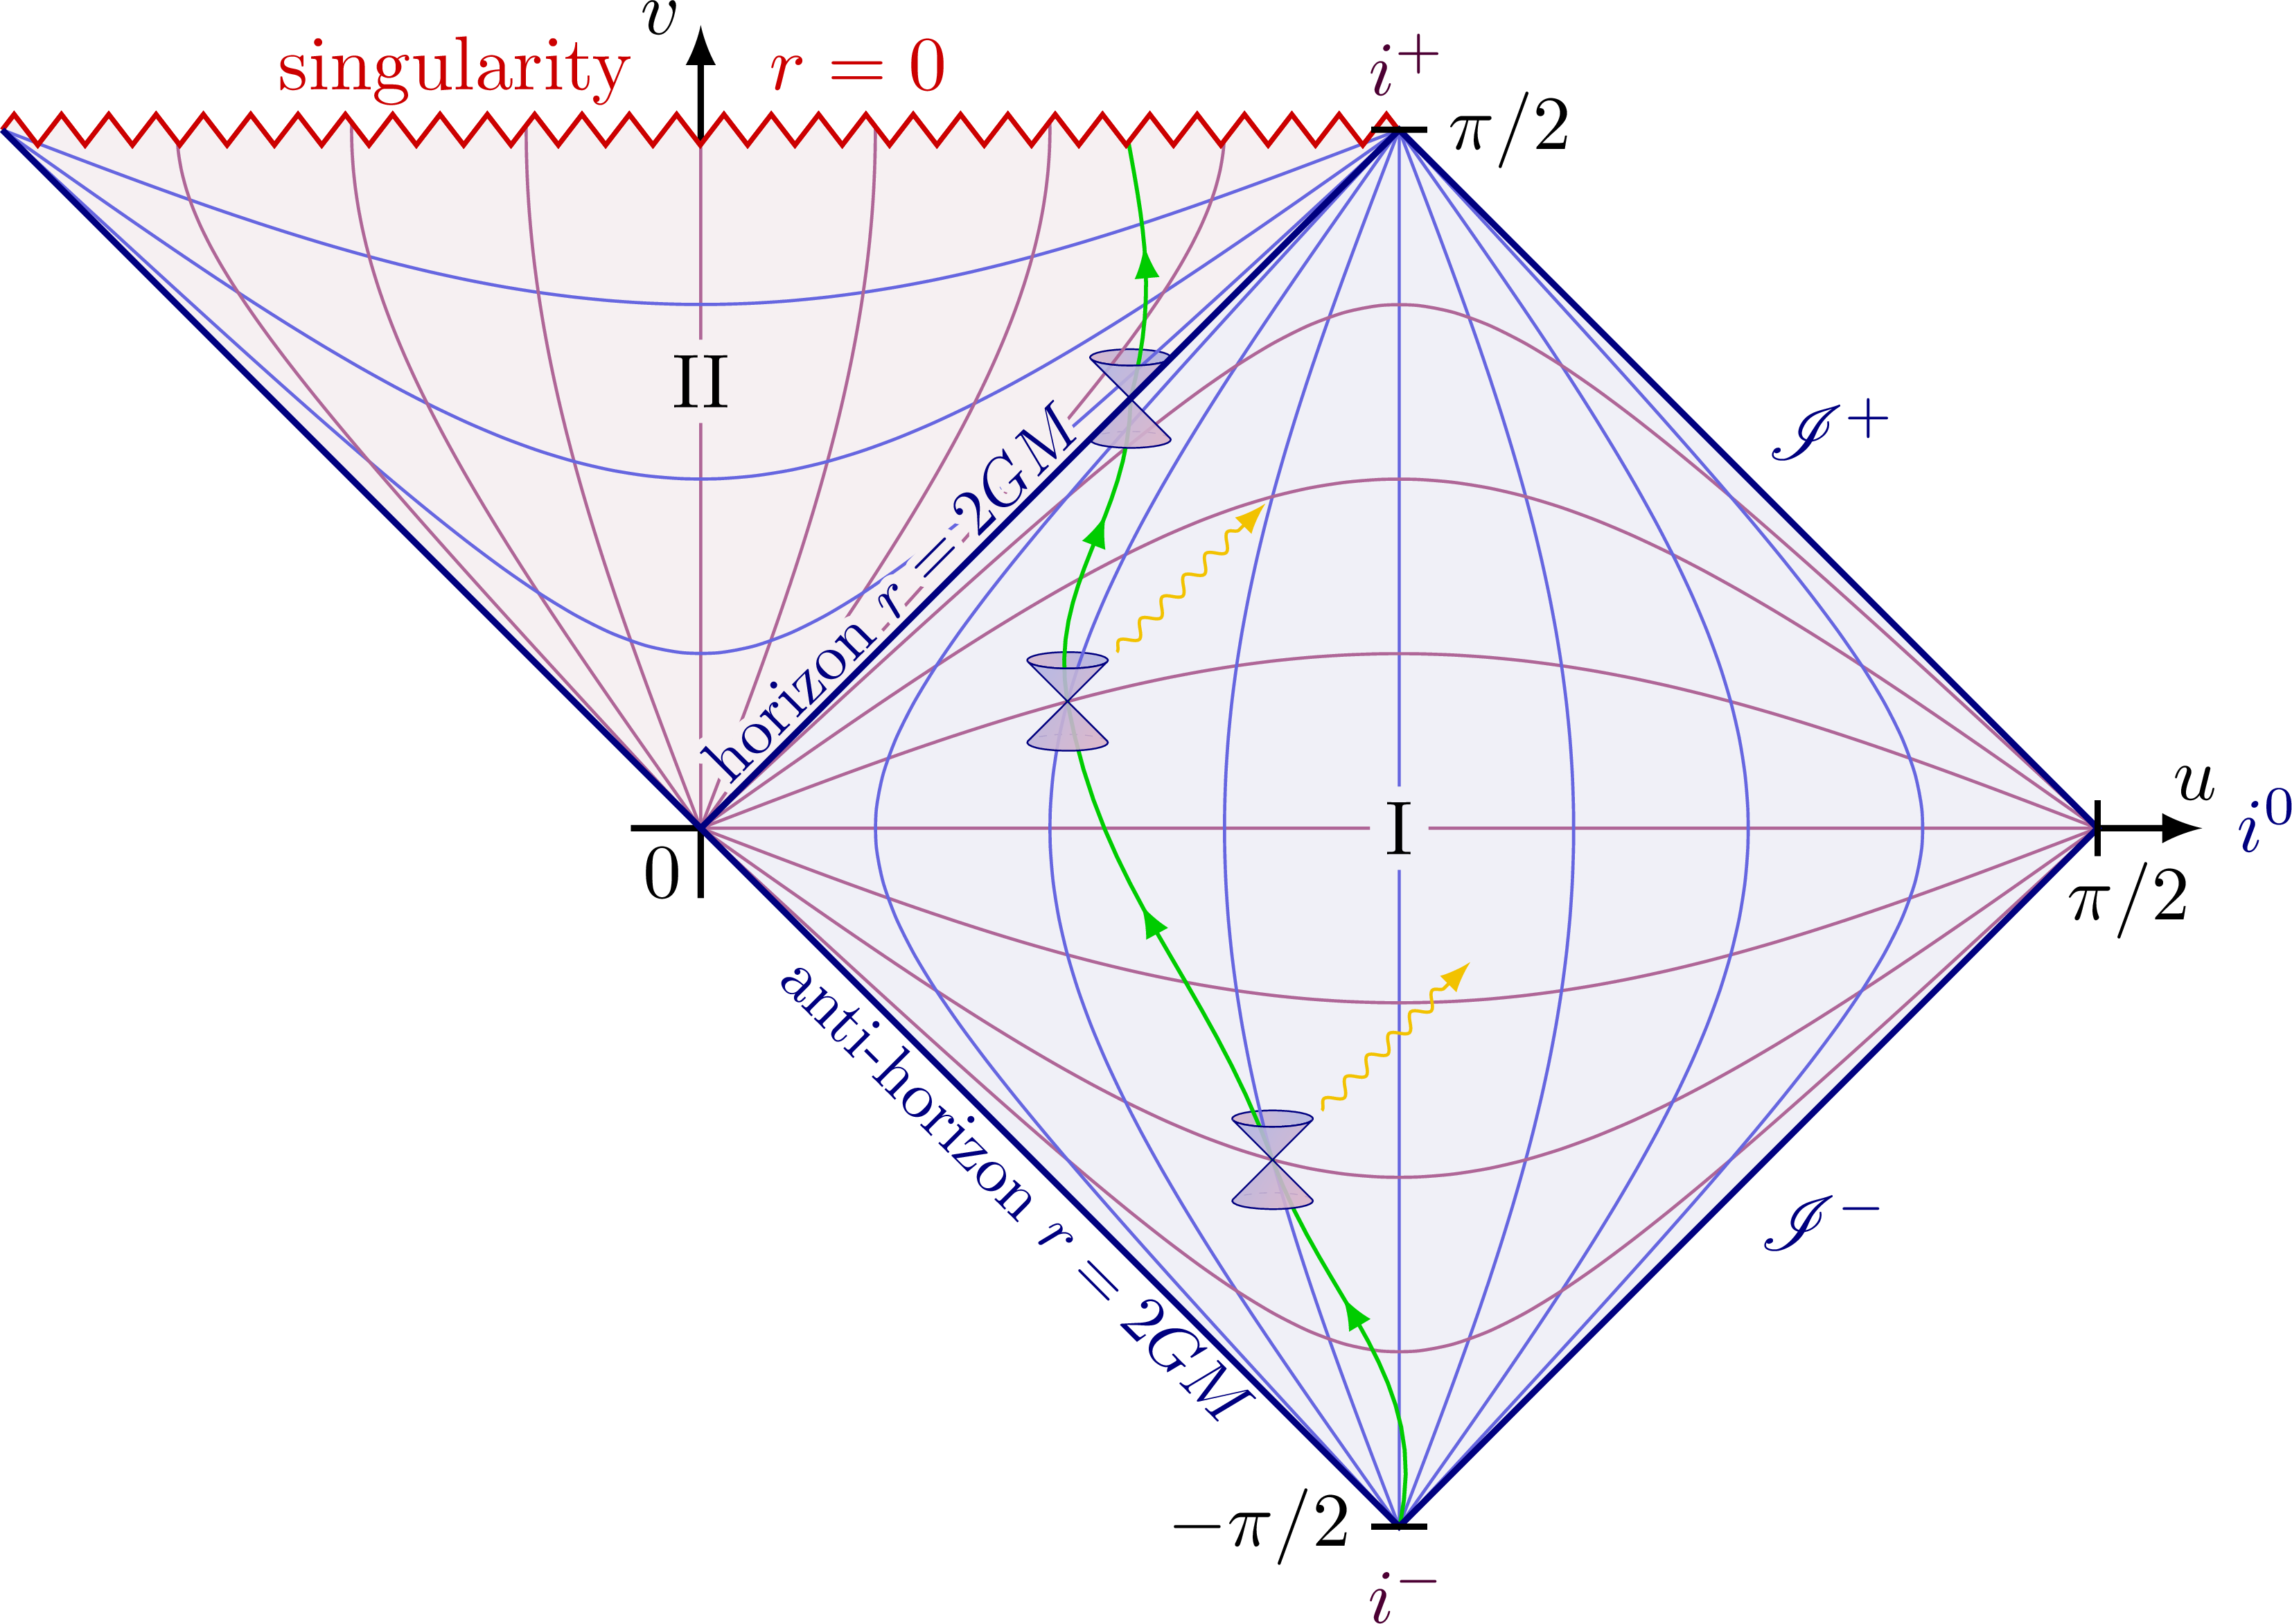
\includegraphics[alt={{Penrose diagram of the Schwarzschild blackhole solution}}, width=345pt]{images/schwarzschild_penrose_diagram.png}
\end{figure}
Zooming in on the singularity we can introduce two basis elements $\mathbf{B}_1$ and $\mathbf{B}_2$ of the Alexandrov topology one of which is ``$\varepsilon$ from the singularity'' and the second of which is ``$\varepsilon$ from $i^+$"
\begin{figure}[h]
    \centering
    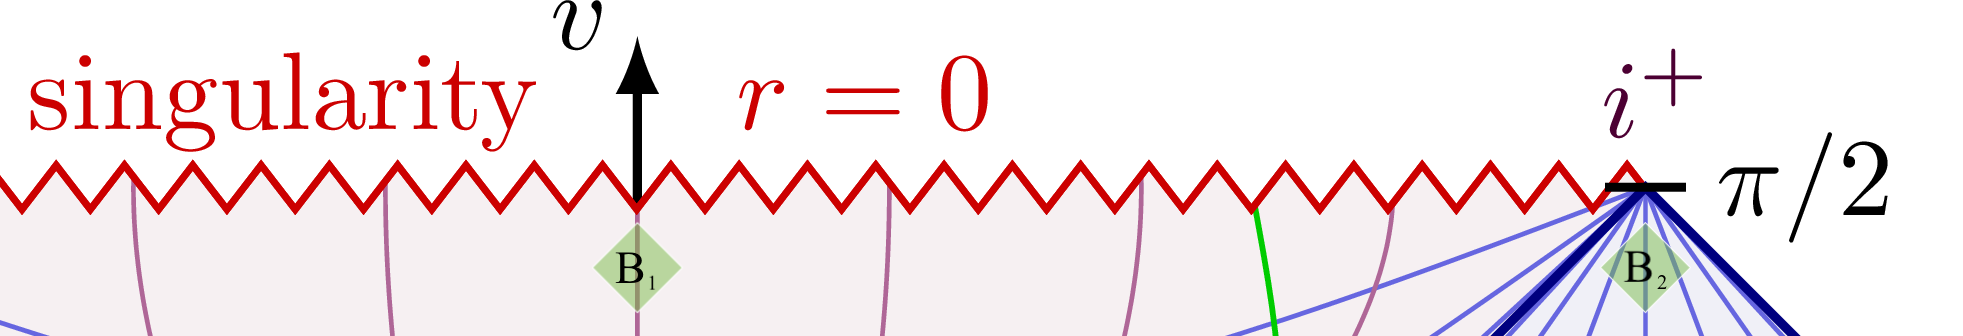
\includegraphics[alt={{Penrose diagram of the Schwarzschild blackhole solution zoomed to singularity, and containing two basis elements}}, width=345pt]{images/schwarzschild_penrose_diagram_zoom1.png}
\end{figure}
What is obvious is that there exists no basis element $\mathbf{B}$ of the Alexandrov topology that contains both $\mathbf{B}_1$ and $\mathbf{B}_2$ as it would have to extend beyond the singularity off of $M_{BH}$ which is of course not allowed.

As a result of this, one can not employ the isotony axiom, the only tool one has, to place $\mathfrak{U}(\mathbf{B}_1)$ and $\mathfrak{U}(\mathbf{B}_2)$ in a larger algebra, an algebra in which addition and multiplication of their elements would make sense. This is exactly where curved spacetime parts ways with Minkowski spacetime: there, any two basis elements lie in a common, larger basis element (Section~\ref{sctn:quasilocal-algebra}), so isotony always places their algebras in a common algebra, and Axiom 3 can be stated in it.

This implies that the set-theoretic union of all $\mathfrak{U}(\mathbf{B})$ over all basis elements $\mathbf{B}$ of the Alexandrov topology on $M_{BH}$ is not a normed *-algebra. This in turn implies that the construction of the quasilocal algebra fails\footnote{This argument can be formalized. However, doing so doesn't provide any insight beyond what's presented by this informal argument. Hence, we omitted the formal argument.} for $M_{BH}$.

For any two basis elements $\mathbf{B}_1$ and $\mathbf{B}_2$ of the Alexandrov topology on a generic Lorentzian spacetime $M$ the best one can hope for is that there exists a third element $\mathbf{B}$ of the Alexandrov topology such that $\mathbf{B}_1, \mathbf{B}_2 \subseteq \mathbf{B}$. However, there is no guarantee that such a $\mathbf{B}$ exists in a Lorentzian spacetime.

All that being said, we can still state a variation of Axiom 3 (Local Commutativity) that applies to a Lorentzian spacetime.

\subsection{Axiom 3 (Local Commutativity)}
The variation of Axiom 3 (Local Commutativity) as applied to Lorentzian spacetime is the following:

\begin{axiom}[Local Commutativity]
    Let $\mathbf{B}_1$ and $\mathbf{B}_2$ be any two basis elements of the Alexandrov topology on a Lorentzian spacetime, i.e. any two sets of the form $I^+(p_1) \cap I^-(q_1)$ and $I^+(p_2) \cap I^-(q_2)$.
    
    If $\mathbf{B_1}$ and $\mathbf{B_2}$ are completely spacelike, for any basis element $\mathbf{B}$ such that $\mathbf{B_1}, \mathbf{B_2} \subseteq \mathbf{B}$ the algebras $\mathfrak{U}(\mathbf{B_1})$ and $\mathfrak{U}(\mathbf{B_2})$ commute in the C*-algebra $\mathfrak{U}(\mathbf{B})$, i.e. for any $a_1$ in $\mathfrak{U}(\mathbf{B_1})$ and $a_2$ in $\mathfrak{U}(\mathbf{B_2})$ we have
    \begin{align}
        i(a_1) i(a_2) - i(a_2) i(a_1) = 0
    \end{align}
    in the C*-algebra $\mathfrak{U}(\mathbf{B})$, where $i$ is the unital *-monomorphism Axiom 2 (Isotony).
    
    If no such $\mathbf{B}$ exists, then it simply doesn't make sense to consider if $\mathfrak{U}(\mathbf{B_1})$ and $\mathfrak{U}(\mathbf{B_2})$ commute as they are not in the same algebra.
\end{axiom}

While having the commutation status of $\mathfrak{U}(\mathbf{B_1})$ and $\mathfrak{U}(\mathbf{B_2})$ sometimes being undefined seems ``odd'' at first. It's actually not ``odd'' at all. The commutation status of $\mathfrak{U}(\mathbf{B_1})$ and $\mathfrak{U}(\mathbf{B_2})$ is only undefined when it's impossible to conduct an experiment that determines if they commute. This makes complete sense.

\section{Axiom 4 (Local Algebra)}\label{sctn:axiom-4-(local-algebra)}
The axiom we are about to present also changes slightly from its analog Axiom 4 (Quasilocal Algebra) on Minkowski spacetime. The reason for the change, as was the reason for the change in Axiom 3 (Local Commutativity), is the fact that there is no such thing as a quasilocal algebra on a generic Lorentzian spacetime.

Before we state the next axiom for Lorentzian spacetimes, we need to, as in the case of Minkowski spacetime, present a definition used in the statement of the axiom.

This definition relies upon the fact, which one may check, that the GNS construction for a state $\omega$ on a C*-algebra $\mathfrak{U}(\mathbf{B})$, where $\mathbf{B}$ is an element of the Alexandrov topology on the Lorentzian spacetime $M$, works just as in the case of AQFT in Minkowski spacetime.

\begin{definition}[Local Observable]
    For Lorentzian spacetime $M$ the image $\pi_\omega(a)$ of a self-adjoint member $a$ of the local algebra $\mathfrak{U}(\mathbf{B})$ under the GNS *-homomorphism $\pi_\omega$ of a state $\omega$ on $\mathfrak{U}(\mathbf{B})$ is self-adjoint and thus corresponds to an ``observable''. Any ``observable'' corresponding to such a self-adjoint $\pi_\omega(a)$ is called a \textit{local observable}.
\end{definition}

Using this definition we can state the axiom

\begin{axiom}[Local Algebra]
    All ``observables'' are local observables.
\end{axiom}

As shown in Section~\ref{sctn:all-observables-of-interest}, this axiom is essentially the statement that there exist ``observables'' that are not local observables, but such ``observables'' are ``experimentally indistinguishable'' from local observables and thus can be ignored.

\section{Axiom 5 (Isometric Covariance)}\label{sctn:axiom-5-(isometric-covariance)}
Now we present the final, and most interesting, axiom in the case of Lorentzian spacetimes.

The interesting aspect of this theorem is understanding what replaces the inhomogeneous Lorentz group connected to the identity, which appears in the Minkowski spacetime analog. One might think to replace it with diffeomorphisms of a Lorentzian spacetime. However, this isn't the correct analog.

Lorentzian spacetimes can admit diffeomorphisms that are not connected to the identity. (For example, in two dimensions \href{https://en.wikipedia.org/wiki/Dehn_twist}{Dehn twists} aren't connected to the identity.) So, if we want to ``mirror'' Axiom 5 (Lorentz Covariance) from the Minkowski case (which only considers group elements connected to the identity), we should limit the diffeomorphisms we employ.

So the ``natural'' choice seems to be the set of diffeomorphisms that are connected to the identity. However, this also isn't the correct analog.

Consider the case of Minkowski spacetime and the analogous axiom Axiom 5 (Lorentz Covariance). There the inhomogeneous Lorentz group connected to the identity is used. Under that group the Minkowski metric is invariant
\begin{align}
    \eta \longrightarrow \eta.
\end{align}
So instead of diffeomorphisms connected to the identity being used, what's being used here are isometries connected to the identity, i.e. diffeomorphism connected to the identity that leave the metric invariant.

So in the current case of a Lorentzian spacetime what we should be using are isometries connected to the identity. Using this, the axiom takes the following form:

(Formalization remark.) An isometry connected to the identity automatically preserves the time orientation, so ``isometries connected to the identity'' is the same group as ``identity-component isometries that preserve the future orientation''. The Lean formalization works with the latter description: it intersects the identity component with the (explicitly orientation-preserving) subgroup, because the inclusion of the identity component into the orientation-preserving isometries relies on a Myers--Steenrod-type rigidity result that Mathlib does not provide. This is an implementation choice only; it does not alter the mathematical content of the axiom below.

\begin{axiom}[Isometric Covariance]
    Let $\mathbf{B}$ be any basis element of the Alexandrov topology on a Lorentzian spacetime $M$, i.e. any set of the form $I^+(p) \cap I^-(q)$.
    
    A member $\varphi$ of the group of isometries of $M$ connected to the identity acts on $\mathfrak{U}(\mathbf{B})$ as follows
    \begin{align}
        \alpha_\varphi : \mathfrak{U}(\mathbf{B}) &\longrightarrow \mathfrak{U}(\varphi(\mathbf{B})) \\
                                   a              &\longmapsto     \alpha_\varphi(a)
    \end{align}
    where $\varphi(\mathbf{B})$ is the image of the basis element $\mathbf{B}$ under the isometry $\varphi$ and $\alpha_\varphi$ is a unital *-isomorphism generated by $\varphi$. The map $\alpha_\varphi$ is such that (1) for the identity isometry $\mathbf{1}$ it satisfies
    \begin{align}
        \alpha_{\mathbf{1}}(a) = a,
    \end{align}
    (2) for all appropriate $a$, $\varphi$, and $\varphi'$ it satisfies
    \begin{align}
        \alpha_{\varphi' \cdot \varphi}(a) = \alpha_{\varphi'}(\alpha_{\varphi}(a)),
    \end{align}
    and (3) for basis elements $\mathbf{B}_\iota \subset \mathbf{B}_\kappa$ and the unital *-monomorphism $i$ of Axiom 2 (Isotony) $\alpha_\varphi$ commutes with $i$. In other words the following diagram

    \begin{center}
        \begin{tikzcd}
            \mathfrak{U}(\mathbf{B}_\kappa) \arrow[r, "\alpha_\varphi"]
            & \mathfrak{U}(\varphi(\mathbf{B}_\kappa)) \\
            \mathfrak{U}(\mathbf{B}_\iota) \arrow[r, "\alpha_\varphi"]  \arrow[u, "i"]
            & \mathfrak{U}(\varphi(\mathbf{B}_\iota))  \arrow[u, "i"]
        \end{tikzcd}
    \end{center}

    commutes.
\end{axiom}


\chapter{Haag Kastler Axioms Blueprint}\label{chptr:haag-kastler-axioms-blueprint}
With all the original Haag Kastler Axioms unpacked, we are now in a position to ``sharpen'' their formulation.

However, before even stating the ``sharpened'' axioms, the first thing we need to do is to define a number of terms to a level amenable to auto-formalization and also prove a number of theorems.

The Lean formalization accompanying this chapter builds against Lean v4.35.0 and Mathlib v4.35.0.

\section{GNS Construction Details}\label{sctn:gns-construction-details}
Here we will state and prove the GNS Construction Theorem, which we make use of in the axioms we present later.

We generally follow the clear, straightforward presentation in \href{https://arxiv.org/abs/2410.16599}{Entanglement in Algebraic Quantum Field Theories}.

\subsection{GNS Construction Theorem}
In this section we will state the GNS Construction Theorem, which we prove in subsequent sections.

Before stating the theorem we'll need to introduce terminology that appears in the theorem's statement. We begin with the definition of "state" and some closely associated terms.

\begin{definition}[State]
    \label{def:state}
    \lean{Physicslib4.GNS.State, Physicslib4.GNS.State.IsFaithful}
    \leanfile{Physicslib4/GNS/Basic.lean}
    \leanok
    Let $\mathfrak{U}$ be an abstract C*-algebra. A \textit{state} is an element $\omega$ of the dual space $\mathfrak{U}^*$ that is
    \begin{itemize}
        \item \textit{Positive} - for any $a \in \mathfrak{U}$ we have $0 \le \omega(a^*a)$ and
        \item \textit{Normalized} - the operator norm satisfies $\| \omega \|=1$.
    \end{itemize}
    Furthermore, a state $\omega$ is said to be \textit{faithful} if for any non-zero $a$ in $\mathfrak{U}$, it follows that $0 < \omega(a^*a)$.
\end{definition}

We will also have need of the term "cyclic vector".

\begin{definition}[Cyclic Vector]
    \label{def:cyclic-vector}
    \lean{Physicslib4.GNS.IsCyclicVector}
    \leanfile{Physicslib4/GNS/Basic.lean}
    \leanok
    Let $\mathcal{A}$ be an algebra represented by the bounded operators $\pi(\mathcal{A})$ on the Hilbert space $\mathcal{H}$. A vector $\Omega$ in $\mathcal{H}$ is said to be a \textit{cyclic vector} if the set
    \begin{align}
        \{ A\Omega : A \in \pi(\mathcal{A}) \}
    \end{align}
    is dense in $\mathcal{H}$.
\end{definition}

With this terminology we are then able to state the GNS Construction Theorem.

\begin{theorem}[GNS Construction Theorem]
    \label{thrm:gns-construction-theorem}
    \lean{Physicslib4.GNS.gns_construction, Physicslib4.GNS.gns_unique}
    \leanfile{Physicslib4/GNS/Construction.lean}
    \uses{def:state, def:cyclic-vector}
    \leanok
    Let $\omega$ be a state over a unital C*-algebra $\mathfrak{U}$. One can then construct a Hilbert space $\mathcal{H}_\omega$ and *-representation $\pi_\omega$ of $\mathfrak{U}$ by bounded operators on $\mathcal{H}_\omega$ such that
    \begin{align}
        \pi_\omega(a^*) = \pi_\omega(a)^\dagger.
    \end{align}
    As $\mathfrak{U}$ is unital, there exists a cyclic vector $\Omega$ in $\mathcal{H}_\omega$ for the representation $\pi_\omega$ such that
    \begin{align}
        \omega(a) = \left<\Omega, \pi_\omega(a)\Omega\right>_{\mathcal{H}_\omega}.
    \end{align}
    The triple $(\mathcal{H}_\omega, \pi_\omega, \Omega)$ is called the \textit{GNS triple} associated to $(\mathfrak{U}, \omega)$ or the \textit{cyclic representation} of $(\mathfrak{U}, \omega)$. Furthermore, if $\omega$ is a faithful state, then the *-representation $\pi_\omega$ is faithful. In addition the GNS triple associated to $(\mathfrak{U}, \omega)$ is unique up to unitary equivalence.
\end{theorem}
\begin{proof}
    \leanok
    \uses{def:state, def:cyclic-vector, lmm:cauchy-schwarz-inequality, lmm:lmm1, lmm:lmm2}
This proof has five parts: (1) the construction of the GNS Hilbert space $\mathcal{H}_\omega$, (2) the construction of the *-representation $\pi_\omega$, (3) the construction of the cyclic vector $\Omega$ in $\mathcal{H}_\omega$, (4) the proof that the *-representation $\pi_\omega$ is faithful, and (5) the proof of uniqueness up to unitary equivalence. Each part corresponds to one of the parts below.

\noindent\textbf{Construction of the GNS Hilbert Space.}
We'll construct the GNS Hilbert space $\mathcal{H}_\omega$ from the C*-algebra $\mathfrak{U}$ itself, modifying $\mathfrak{U}$ as needed to obtain the desired $\mathcal{H}_\omega$.

Let's start by attempting to place an inner product on $\mathfrak{U}$. Naively one might hope the following defines an inner product
\begin{align}
    \left< a, b \right> \equiv \omega(a^*b)
\end{align}
on $\mathfrak{U}$. Unfortunately it doesn't. Let's examine why this fails.

Consider the set
\begin{align}
    \mathcal{N} \equiv \{ n \in \mathfrak{U} : \omega(n^*n) = 0 \}.
\end{align}
Generically $\omega$ isn't faithful. Thus in $\mathcal{N}$ there exist non-zero $n$. For such $n$ one has
\begin{align}
    \left< n, n \right> \equiv \omega(n^*n) = 0.
\end{align}
Hence, there are non-zero $n$ in $\mathfrak{U}$ such that $\left< n, n \right> = 0$. The existence of such $n$ proves that our naive inner product on $\mathfrak{U}$
\begin{align}
    \left< a, b \right> \equiv \omega(a^*b)
\end{align}
actually isn't an inner product. However, the form $\mathcal{N}$ takes gives us a hint as to how to repair this naive inner product.

In particular, if we quotient $\mathfrak{U}$ by $\mathcal{N}$ we may rid ourselves of the problem we encountered above and hopefully be able to construct an inner product on $\mathfrak{U} / \mathcal{N}$ and its completion. We'll see this plan actually works.

However, before being able to see this plan through we'll need to take a quick detour and prove a few needed results, which are stated and proved separately below.

The most famous of these results is the Cauchy-Schwarz Inequality (\ref{lmm:cauchy-schwarz-inequality}).

The next result we need to prove is the equality $\mathcal{N} = \mathcal{N}_1$ of the two null sets (\ref{lmm:lmm1}).

Next we will prove $\mathcal{N}$ is a closed, linear subspace of $\mathfrak{U}$ (\ref{lmm:lmm2}). Establishing this will allow us to take the quotient of $\mathfrak{U}$ by $\mathcal{N}$.

As we have established that $\mathcal{N}$ is a closed, linear subspace of $\mathfrak{U}$, we can now take the quotient of $\mathfrak{U}$ by $\mathcal{N}$. Elements of the quotient $\mathfrak{U} / \mathcal{N}$ are equivalence classes of the form
\begin{align}
    [a] \equiv \{ a + n : n \in \mathcal{N} \}
\end{align}
with the zero vector in $\mathfrak{U} / \mathcal{N}$ given by
\begin{align}
    [0] \equiv \{ n : n \in \mathcal{N} \}.
\end{align}
On $\mathfrak{U} / \mathcal{N}$ we can introduce an inner product
\begin{align}
    \left<[a], [b]\right> \equiv \omega(a^*b)
\end{align}
motivated by our naive attempt at placing an inner product on $\mathfrak{U}$. This inner product is well-defined on $\mathfrak{U} / \mathcal{N}$ as one can see from its invariance under $a \rightarrow a + n$ where $n$ is in $\mathcal{N}$,
\begin{align}
    \omega((a + n)^*b) = \omega(a^*b) + \omega(n^*b) = \omega(a^*b) + \overline{\omega(b^*n)} = \omega(a^*b).
\end{align}
In this the first equality follows from $\omega$ being linear, the second from our previous result $\omega(n^*b) = \overline{\omega(b^*n)}$, and the final from our previous result $\mathcal{N} = \mathcal{N}_1$. A similar argument using $\mathcal{N} = \mathcal{N}_1$ yields invariance under $b \rightarrow b + n$ too.

Furthermore, the inner product
\begin{align}
    \left<[a], [b]\right> \equiv \omega(a^*b)
\end{align}
on $\mathfrak{U} / \mathcal{N}$ doesn't suffer from the same problem that our naive inner product on $\mathfrak{U}$ did. In particular, one can easily prove
\begin{align}
    \left<[a], [a]\right> = 0
\end{align}
if and only if $[a] = [0]$. This is essentially by construction.

The final step in going from $\mathfrak{U} / \mathcal{N}$ to the Hilbert space $\mathcal{H}_\omega$ consists of completing $\mathfrak{U} / \mathcal{N}$ in the norm defined by the inner product above. As this is standard, we will not present the details here. The completion of $\mathfrak{U} / \mathcal{N}$ in this norm is the Hilbert space $\mathcal{H}_\omega$ of the GNS Construction Theorem.

\noindent\textbf{Construction of the GNS Representation.}
Next we will construct $\pi_\omega$ the *-representation of $\mathfrak{U}$ by bounded operators on $\mathcal{H}_\omega$. This will be much easier than the construction of $\mathcal{H}_\omega$.

By construction we can consider $\mathfrak{U} / \mathcal{N}$ as dense in $\mathcal{H}_\omega$. On this dense subset we define the action of $\pi_\omega$ the *-representation of $\mathfrak{U}$ on $\mathfrak{U} / \mathcal{N}$ as follows
\begin{align}
    \pi_\omega(a)[z] \equiv [az]
\end{align}
where $[z]$ is an arbitrary element of $\mathfrak{U} / \mathcal{N}$.

This definition of $\pi_\omega$ on $\mathfrak{U} / \mathcal{N}$ is well-defined as for any other member of the equivalence class $[z]$ of the form $[z + n]$ one has
\begin{align}
    \pi_\omega(a)[z + n] = [az + an] = [az],
\end{align}
where the second equality follows from our previous result $\mathcal{N}_1 = \mathcal{N}$. In other words, $\pi_\omega$ is well-defined as $\mathcal{N}$ is a left-ideal in $\mathfrak{U}$.

Furthermore, it trivially follows from the definition of $\pi_\omega$ that it is linear and an algebraic morphism. So it remains to prove that $\pi_\omega$ is bounded and also a *-morphism.

Let us first prove that $\pi_\omega$ is bounded.

Consider a non-zero $[z]$ in $\mathfrak{U} / \mathcal{N}$. Simply applying definitions one has
\begin{align}
    \|\pi_\omega(a)[z]\|^2 &= \|[az]\|^2 \\
                           &= \left<[az], [az]\right> \\
                           &= \omega((az)^*(az)) \\
                           &= \omega(z^*(a^*a)z) \\
                           &= \frac{\omega(z^*(a^*a)z)}{\omega(z^*z)} \omega(z^*z) \\
                           &= \frac{\omega(z^*(a^*a)z)}{\omega(z^*z)} \|[z]\|^2.
\end{align}
With that last equation in mind let us define the map $\phi$ acting on $\mathfrak{U}$ by
\begin{align}
    \phi(a) \equiv \frac{\omega(z^*az)}{\omega(z^*z)}.
\end{align}
One can easily check that $\phi$ when acting on $\mathfrak{U}$ is linear and positive as
\begin{align}
    \phi(c^*c) = \frac{\omega(z^*(c^*c)z)}{\omega(z^*z)} = \frac{\omega((cz)^*(cz))}{\omega(z^*z)} \ge 0
\end{align}
as a result of $\omega$ being positive.

Now as $\phi$ is a positive, linear function on the unital C*-algebra $\mathfrak{U}$ we can invoke the theorem (Chapter III Theorem 2.2.9 of \href{https://doi.org/10.1007/978-3-642-61458-3}{Haag})

\begin{quote}
    \textit{Theorem.} A positive, linear operator $\phi$ on a unital Banach *-algebra $\mathcal{A}$ is bounded and satisfies
    \begin{align}
        \|\phi\| = \phi(\mathbf{1})
    \end{align}
    where $\phi(\mathbf{1})$ is $\phi$ acting on the unit $\mathbf{1}$ of $\mathcal{A}$.
\end{quote}

\noindent to prove that $\|\phi\| = \phi(\mathbf{1})$. A short computation finds
\begin{align}
    \phi(\mathbf{1}) = \frac{\omega(z^*\mathbf{1}z)}{\omega(z^*z)} = 1
\end{align}
proving $\|\phi\|=1$, i.e. $\phi$ is normalized. As $\phi$ is a linear, positive, normalized operator on the unital C*-algebra $\mathfrak{U}$, it is indeed a state.

Now as $\phi$ is normalized and thus $\|\phi\|=1$, the definition of the norm $\|\phi\|$ implies
\begin{align}
    \|\phi(c)\| \le \|\phi\| \, \|c\| = \|c\|.
\end{align}
This along with our previous derivation gives
\begin{align}
    \|\pi_\omega(a)[z]\|^2 &= \phi(a^*a) \|[z]\|^2 \\
                           &\le \|\phi\| \, \|a^*a\| \, \|[z]\|^2 \\
                           &=  \|a^*a\| \, \|[z]\|^2 \\
                           &= \|a\|^2 \, \|[z]\|^2.
\end{align}
Using the definition of the norm $\|\pi_\omega(a)\|$ this equation then implies
\begin{align}
    \|\pi_\omega(a)\| \le \|a\|
\end{align}
which is the statement that $\pi_\omega(a)$ is a bounded operator on $\mathfrak{U} / \mathcal{N}$.

Thus using the following standard theorem (Theorem A.36 \href{https://doi.org/10.1007/978-1-4614-7116-5}{Hall})

\begin{quote}
    \textit{Bounded Linear Transformation Theorem.} Let $V_1$ be a normed space and $V_2$ a Banach space. Suppose $W$ is a dense subspace of $V_1$ and $T: W \rightarrow V_2$ is a bounded linear map. Then there exists a unique bounded linear map $\widetilde{T}: V_1 \rightarrow V_2$ such that $\widetilde{T}|_W = T$. Furthermore, the norm of $\widetilde{T}$ equals the norm of $T$.
\end{quote}

\noindent one can extend $\pi_\omega$ from the dense subset $\mathfrak{U} / \mathcal{N}$ of $\mathcal{H}_\omega$ to all of $\mathcal{H}_\omega$. We do so and use the same notation $\pi_\omega$ for this extension.

Finally we need to prove that $\pi_\omega$ is not only an algebraic morphism but is a *-morphism. Thankfully this is relatively simple.

For $[x]$ and $[y]$ in $\mathfrak{U} / \mathcal{N}$ and $a$ in $\mathfrak{U}$, we have
\begin{align}
    \left<[x], \pi_\omega(a^*)[y]\right> &= \left<[x], [a^*y]\right> \\
                                         &= \omega(x^*a^*y) \\
                                         &= \omega((ax)^*y) \\
                                         &= \left<[ax], [y]\right> \\
                                         &= \left<\pi_\omega(a)[x], [y]\right> \\
                                         &= \left<[x], \pi_\omega(a)^\dagger [y]\right>
\end{align}
Hence, $\pi_\omega(a^*) = \pi_\omega(a)^\dagger$ and $\pi_\omega$ is a *-morphism.

\noindent\textbf{Construction of the Cyclic Vector.}
Our next task is to construct the cyclic vector $\Omega$. This is relatively straightforward.

As $\mathfrak{U}$ is unital we can make the definition
\begin{align}
    \Omega \equiv [\mathbf{1}].
\end{align}
Tracing definitions we have
\begin{align}
    \{\pi_\omega(a)\Omega : a \in \mathfrak{U}\} = \{[a] : a \in \mathfrak{U}\} = \mathfrak{U} / \mathcal{N}.
\end{align}
As $\mathfrak{U} / \mathcal{N}$ is dense in $\mathcal{H}_\omega$, this implies that $\Omega$ is a cyclic vector in $\mathcal{H}_\omega$ for the representation $\pi_\omega$, the property claimed of $\Omega$ in the GNS Construction Theorem.

In addition tracing definitions gives
\begin{align}
    \left<\Omega, \pi_\omega(a)\Omega\right> = \left<[\mathbf{1}], \pi_\omega(a)[\mathbf{1}]\right> = \left<[\mathbf{1}], [a]\right> = \omega(\mathbf{1}a) = \omega(a)
\end{align}
which proves another relation
\begin{align}
    \omega(a) = \left<\Omega, \pi_\omega(a)\Omega\right>
\end{align}
claimed in the GNS Construction Theorem.

\noindent\textbf{Faithfulness of the GNS Representation.}
Now we are going to prove the *-representation $\pi_\omega$ is faithful if $\omega$ is a faithful state.

For this section of the proof, assume that $\omega$ is a faithful state.

To prove that $\pi_\omega$ is a faithful representation, we must prove that $\ker \pi_\omega = \{0\}$. In other words, we must prove that $\pi_\omega(a) = 0$ implies that $a=0$.

Assume that $\pi_\omega(a) = 0$. Thus we have
\begin{align}
    0 = \left<\pi_\omega(a)\Omega, \pi_\omega(a)\Omega\right> = \omega(a^*a).
\end{align}
As $\omega$ is assumed faithful in this section of the proof, this implies that $a=0$. This in turn implies $\ker \pi_\omega = \{0\}$, which proves that if $\omega$ is faithful, then $\pi_\omega$ is faithful, the desired result.

\noindent\textbf{Uniqueness up to Unitary Equivalence.}
Finally to complete the proof of the GNS Construction Theorem we now prove that the GNS triple associated to $(\mathfrak{U}, \omega)$ is unique up to unitary equivalence.

To that end let $(\mathcal{H}_\omega', \pi_\omega', \Omega')$ be a second GNS triple associated to $(\mathfrak{U}, \omega)$. (This implies, in particular, that the inner product on $\mathcal{H}_\omega'$ is given by $\omega$.) Then define an operator $U$ by
\begin{align}
    U\pi_\omega(a)\Omega \equiv \pi_\omega(a)'\Omega'.
\end{align}
The operator $U$ is obviously linear. Furthermore, as $\Omega$ and $\Omega'$ are cyclic, the domain of $U$ is dense in $\mathcal{H}_\omega$ and its range is dense in $\mathcal{H}_\omega'$. Now, as a result of chasing definitions
\begin{align}
    \left< U\pi_\omega(a)\Omega, U\pi_\omega(b)\Omega \right>' &= \left<\pi_\omega(a)'\Omega', \pi_\omega(b)'\Omega'\right>' \\
                                                               &= \omega(a^*b) \\
                                                               &= \left<\pi_\omega(a)\Omega, \pi_\omega(b)\Omega\right>
\end{align}
we find that $U$ preserves the inner product and is thus bounded. Furthermore, as $U$ preserves the inner product on its dense domain and dense range, it's also unitary there.

As $U$ is bounded on its dense domain, the Bounded Linear Transformation Theorem (Theorem A.36 \href{https://doi.org/10.1007/978-1-4614-7116-5}{Hall})

\begin{quote}
    \textit{Bounded Linear Transformation Theorem.} Let $V_1$ be a normed space and $V_2$ a Banach space. Suppose $W$ is a dense subspace of $V_1$ and $T: W \rightarrow V_2$ is a bounded linear map. Then there exists a unique bounded linear map $\widetilde{T}: V_1 \rightarrow V_2$ such that $\widetilde{T}|_W = T$. Furthermore, the norm of $\widetilde{T}$ equals the norm of $T$.
\end{quote}

\noindent can be used to extend the domain of $U$ to all of $\mathcal{H}_\omega$. This gives a well-defined, unitary map from $\mathcal{H}_\omega$ to $\mathcal{H}_\omega'$ that we also denote by $U : \mathcal{H}_\omega \rightarrow \mathcal{H}_\omega'$.

Now, the definition of $U$
\begin{align}
    U\pi_\omega(a)\Omega = \pi_\omega(a)'\Omega'.
\end{align}
gives for the case $a = \mathbf{1}$
\begin{align}
    U\Omega = \Omega'.
\end{align}
Hence, the fact that $U$ is unitary and thus $U^{-1}$ is well-defined gives
\begin{align}
    \left< U\pi_\omega(a)\Omega, U\pi_\omega(b)\Omega \right>' &= \left< U\pi_\omega(a)U^{-1}U\Omega, U\pi_\omega(b)\Omega \right>' \\
                                                               &= \left< U\pi_\omega(a)U^{-1}U\Omega, \pi_\omega(b)'\Omega' \right>' \\
                                                               &= \left< U\pi_\omega(a)U^{-1}\Omega', \pi_\omega(b)'\Omega' \right>'.
\end{align}
However, the definition of $U$ implies
\begin{align}
    \left< U\pi_\omega(a)\Omega, U\pi_\omega(b)\Omega \right>' = \left<\pi_\omega(a)'\Omega', \pi_\omega(b)'\Omega'\right>'.
\end{align}
Thus the previous two equations imply
\begin{align}
    \left< U\pi_\omega(a)U^{-1}\Omega', \pi_\omega(b)'\Omega' \right>' = \left<\pi_\omega(a)'\Omega', \pi_\omega(b)'\Omega'\right>'.
\end{align}
As a result of cyclicity of $\Omega'$ this implies that
\begin{align}
    U\pi_\omega(a)U^{-1}\Omega' = \pi_\omega(a)'\Omega'.
\end{align}
To complete the proof we must first show that $U\pi_\omega(a)U^{-1}$ and $\pi_\omega(a)'$ agree not only on $\Omega'$, but also on $\pi_\omega(c)'\Omega'$, which as $\Omega'$ is cyclic is dense in $\mathcal{H}_\omega'$. This can then be used along with the Bounded Linear Transformation Theorem to prove that $U\pi_\omega(a)U^{-1}$ and $\pi_\omega(a)'$ agree on $\mathcal{H}_\omega'$.

Let us first prove that $U\pi_\omega(a)U^{-1}$ and $\pi_\omega(a)'$ agree on $\pi_\omega(c)'\Omega'$. We have
\begin{align}
    U\pi_\omega(a)U^{-1} \pi_\omega(c)'\Omega' &= U\pi_\omega(a)U^{-1} U\pi_\omega(c)U^{-1} \Omega' \\
                                               &= U\pi_\omega(a)\pi_\omega(c)U^{-1} \Omega' \\
                                               &= U\pi_\omega(ac)U^{-1} \Omega' \\
                                               &= \pi_\omega(ac)' \Omega' \\
                                               &= \pi_\omega(a)'\pi_\omega(c)' \Omega'
\end{align}
Thus $U\pi_\omega(a)U^{-1}$ and $\pi_\omega(a)'$ agree on $\pi_\omega(c)'\Omega'$.

As $\Omega'$ is cyclic, $\pi_\omega(c)'\Omega'$ is dense in $\mathcal{H}_\omega'$, and thus the  Bounded Linear Transformation Theorem (Theorem A.36 \href{https://doi.org/10.1007/978-1-4614-7116-5}{Hall})

\begin{quote}
    \textit{Bounded Linear Transformation Theorem.} Let $V_1$ be a normed space and $V_2$ a Banach space. Suppose $W$ is a dense subspace of $V_1$ and $T: W \rightarrow V_2$ is a bounded linear map. Then there exists a unique bounded linear map $\widetilde{T}: V_1 \rightarrow V_2$ such that $\widetilde{T}|_W = T$. Furthermore, the norm of $\widetilde{T}$ equals the norm of $T$.
\end{quote}

\noindent can be invoked to prove that $U\pi_\omega(a)U^{-1}$ and $\pi_\omega(a)'$ agree on $\mathcal{H}_\omega'$, proving that
\begin{align}
    \pi_\omega(a)' = U\pi_\omega(a)U^{-1},
\end{align}
and two GNS triples associated to $(\mathfrak{U}, \omega)$ can differ at most by a unitary transformation, completing our proof of the GNS Construction Theorem.

\noindent\textit{Formalization note.} The Lean proof of existence (\texttt{gns\_construction}) does not follow the construction above. It takes the Hilbert space to be Mathlib's GNS space of the positive linear functional $\omega$ (\texttt{PositiveLinearMap.GNS}, the completion of the quotient \texttt{PositiveLinearMap.PreGNS}), together with Mathlib's left-multiplication representation on it. Lemmas~\ref{lmm:cauchy-schwarz-inequality}, \ref{lmm:lmm1} and~\ref{lmm:lmm2} are formalized separately and are not used there.
\end{proof}

\subsection{Auxiliary Results Used in the Proof}
The three results used in the detour of the proof above are stated and proved here.

The most famous of these results is the Cauchy-Schwarz Inequality

\begin{lemma}[Cauchy-Schwarz Inequality]
    \label{lmm:cauchy-schwarz-inequality}
    \lean{Physicslib4.GNS.cauchy_schwarz_inequality, Physicslib4.GNS.omega_star_swap_conj}
    \leanfile{Physicslib4/GNS/CauchySchwarz.lean}
    \uses{def:state}
    \leanok
    Let $\mathcal{A}$ be a *-algebra and $\omega$ a \textit{positive} element of the dual space $\mathcal{A}^*$, i.e. $\omega$ is an element of the dual space $\mathcal{A}^*$ such that for any $a \in \mathcal{A}$ one has $0 \le \omega(a^*a)$. Then
    \begin{align}
        \omega(a^*b) &= \overline{\omega(b^*a)} \\
        |\omega(a^*b)|^2 &\le \omega(a^*a) \omega(b^*b)
    \end{align}
    for all $a$ and $b$ in $\mathcal{A}$.
\end{lemma}
\begin{proof}
\leanok
Positivity of $\omega$ implies that for any $a$ and $b$ in $\mathcal{A}$ and $\lambda \in \mathbb{C}$ one has
\begin{align}
    0 \le \omega\left((\lambda a + b)^*(\lambda a + b)\right).
\end{align}
As $\omega$ is an element of the dual space $\mathcal{A}^*$ and thus linear, this implies
\begin{align}
    0 \le |\lambda|^2\omega(a^*a) + \overline{\lambda}\omega(a^*b) + \lambda\omega(b^*a) + \omega(b^*b).
\end{align}
This inequality then implies both desired results,
\begin{align}
    \omega(a^*b) &= \overline{\omega(b^*a)} \\
    |\omega(a^*b)|^2 &\le \omega(a^*a) \omega(b^*b).
\end{align}
We will prove these one-by-one. Let us first prove this inequality implies $\omega(a^*b) = \overline{\omega(b^*a)}$.

Notice that the inequality is between two real numbers, $0$ and the right-hand side. As $\omega$ is positive, the first and last summands on the right-hand side are obviously real. This then implies
\begin{align}
    \overline{\lambda}\omega(a^*b) + \lambda\omega(b^*a) \in \mathbb{R}.
\end{align}
As $\lambda$ is arbitrary, we are free to choose it to be real, which implies the imaginary parts of $\omega(a^*b)$ and $\omega(b^*a)$ are equal but have the opposite signs.

Similarly, we are free to choose $\lambda$ to be imaginary, which implies that the real parts of $\omega(a^*b)$ and $\omega(b^*a)$ are equal. Together these facts imply the first result
\begin{align}
    \omega(a^*b) = \overline{\omega(b^*a)}.
\end{align}
Let us next prove that our inequality
\begin{align}
    0 \le |\lambda|^2\omega(a^*a) + \overline{\lambda}\omega(a^*b) + \lambda\omega(b^*a) + \omega(b^*b)
\end{align}
implies $\lvert \omega(a^*b) \rvert^2 \le \omega(a^*a) \omega(b^*b)$.

Again, as $\lambda$ is arbitrary, we are free to choose it to extremize the right-hand side of the inequality. Extremizing the right-hand of this inequality with respect to $\overline{\lambda}$ and assuming $\omega(a^*a) \ne 0$ one finds at the extrema
\begin{align}
    \lambda = - \frac{\omega(a^*b)}{\omega(a^*a)}.
\end{align}
Substituting this into the inequality, multiplying by $\omega(a^*a)$ while using the fact that $\omega$ is positive, and using $\omega(a^*b) = \overline{\omega(b^*a)}$, then one obtains
\begin{align}
    0 \le \lvert \omega(a^*b) \rvert^2 - \lvert \omega(a^*b) \rvert^2 - \lvert \omega(a^*b) \rvert^2 + \omega(a^*a) \omega(b^*b)
\end{align}
which implies
\begin{align}
    \lvert \omega(a^*b) \rvert^2 \le \omega(a^*a) \omega(b^*b),
\end{align}
the second desired result under the assumption that $\omega(a^*a) \ne 0$.

If we now allow for the case $\omega(a^*a) = 0$, our inequality reduces to
\begin{align}
    0 \le \overline{\lambda}\omega(a^*b) + \lambda\omega(b^*a) + \omega(b^*b).
\end{align}
Our previous result implies $\omega(b^*a) = \overline{\omega(a^*b)}$. Hence, this inequality takes the form
\begin{align}
    0 \le \overline{\lambda}\omega(a^*b) + \lambda\overline{\omega(a^*b)} + \omega(b^*b) = 2\text{Re}\left(\overline{\lambda} \omega(a^*b)\right) + \omega(b^*b).
\end{align}
Now as $\lambda$ is arbitrary we are free to select it as follows
\begin{align}
    \overline{\lambda} = -r \overline{\omega(a^*b)}
\end{align}
where $0 < r$ is an arbitrary positive real number. Then the previous inequality takes the form
\begin{align}
    0 &\le 2\text{Re}\left(\overline{\lambda} \omega(a^*b)\right) + \omega(b^*b) \\
      &= -2r \lvert \omega(a^*b) \rvert^2 + \omega(b^*b).
\end{align}
Now if we assume for the moment that $0 < \lvert \omega(a^*b) \rvert$, then we can always select $0 < r$ large enough such that this inequality is violated, the $-2r \lvert \omega(a^*b) \rvert^2$ term dominating the $\omega(b^*b)$ term. Hence, it must be the case that $\lvert \omega(a^*b) \rvert = 0$.

Now we have $\omega(a^*a) = 0$ and $\lvert \omega(a^*b) \rvert = 0$. Hence, the desired inequality
\begin{align}
    \lvert \omega(a^*b) \rvert^2 \le \omega(a^*a) \omega(b^*b),
\end{align}
follows trivially, completing our proof.
\end{proof}

The next result we need to prove is:

\begin{lemma}
    \label{lmm:lmm1}
    \lean{Physicslib4.GNS.lmm1, Physicslib4.GNS.nullSet, Physicslib4.GNS.orthSet}
    \leanfile{Physicslib4/GNS/NullSpace.lean}
    \uses{def:state}
    \leanok
    Let $\omega$ be a state over a unital C*-algebra $\mathfrak{U}$. Then the set $\mathcal{N}_1$ defined by
    \begin{align}
        \mathcal{N}_1 \equiv \{ n \in \mathfrak{U} : \omega(b^*n) = 0 \;\; \forall \, b \in \mathfrak{U} \}
    \end{align}
    is equivalent to the set $\mathcal{N}$ defined by
    \begin{align}
        \mathcal{N} \equiv \{ n \in \mathfrak{U} : \omega(n^*n) = 0 \}.
    \end{align}
\end{lemma}
\begin{proof}
\leanok
We will first prove that $\mathcal{N} \subseteq \mathcal{N}_1$. Then we will prove $\mathcal{N}_1 \subseteq \mathcal{N}$. Together these imply $\mathcal{N} = \mathcal{N}_1$, the final desired result.

Let us begin by proving $\mathcal{N} \subseteq \mathcal{N}_1$.

$\mathfrak{U}$ is a C*-algebra and thus a *-algebra. In addition $\omega$ is a state and thus a positive element of the dual space $\mathfrak{U}^*$. Thus, for arbitrary $b$ and $n$ in $\mathfrak{U}$ we can apply the Cauchy-Schwarz inequality to obtain
\begin{align}
    \lvert \omega(b^*n) \rvert^2 \le \omega(b^*b) \omega(n^*n).
\end{align}
Thus if $n$ is in $\mathcal{N}$, and thus satisfies $\omega(n^*n) = 0$, then this inequality implies $\omega(b^*n) = 0$ for all $b$ in $\mathfrak{U}$. This then implies $n$ is in $\mathcal{N}_1$. As $n$ was an arbitrary element of $\mathcal{N}$, this in turn implies that $\mathcal{N} \subseteq \mathcal{N}_1$, the first desired result.

Next let us prove that $\mathcal{N}_1 \subseteq \mathcal{N}$.

Consider an arbitrary $n_1$ in $\mathcal{N}_1$. By definition $\omega(b^*n_1) = 0$ for any $b$ in $\mathfrak{U}$. In particular we can select $b=n_1$. Doing so we have $\omega(n_1^*n_1) = 0$. This then implies $n_1$ is in $\mathcal{N}$. As $n_1$ was an arbitrary element of $\mathcal{N}_1$ this further implies $\mathcal{N}_1 \subseteq \mathcal{N}$, the second desired result.

We have thus proven $\mathcal{N} \subseteq \mathcal{N}_1$ and $\mathcal{N}_1 \subseteq \mathcal{N}$ which together imply $\mathcal{N} = \mathcal{N}_1$, the final desired result.
\end{proof}

Next we will prove $\mathcal{N}$ is a closed, linear subspace of $\mathfrak{U}$. Establishing this will allow us to take the quotient of $\mathfrak{U}$ by $\mathcal{N}$.

\begin{lemma}
    \label{lmm:lmm2}
    \lean{Physicslib4.GNS.lmm2, Physicslib4.GNS.nullSubmodule}
    \leanfile{Physicslib4/GNS/NullSpace.lean}
    \uses{def:state}
    \leanok
    Let $\omega$ be a state over a unital C*-algebra $\mathfrak{U}$. Then the set $\mathcal{N}$ defined by
    \begin{align}
        \mathcal{N} \equiv \{ n \in \mathfrak{U} : \omega(n^*n) = 0 \}.
    \end{align}
    is a closed, linear subspace of $\mathfrak{U}$.
\end{lemma}
\begin{proof}
\leanok
First let us prove that $\mathcal{N}$ is a linear subspace of $\mathfrak{U}$.

Consider arbitrary $n,m \in \mathcal{N}$ and arbitrary $\lambda, \mu \in \mathbb{C}$. As proven above $\mathcal{N} = \mathcal{N}_1$, thus for arbitrary $b \in \mathfrak{U}$, one has
\begin{align}
    \omega(b^*n) &= 0 \\
    \omega(b^*m) &= 0.
\end{align}
Hence, the linearity of $\omega$ then implies
\begin{align}
    \omega(b^*(\lambda n + \mu m)) = \lambda \omega(b^*n) + \mu \omega(b^*m) = 0.
\end{align}
As $b \in \mathfrak{U}$ was arbitrary, this implies that $(\lambda n + \mu m) \in \mathcal{N}_1$. As we previously proved $\mathcal{N} = \mathcal{N}_1$, this in turn implies $(\lambda n + \mu m) \in \mathcal{N}$. Hence $\mathcal{N}$ is a linear subspace of $\mathfrak{U}$, the first desired result.

Next let us prove that $\mathcal{N}$ is a closed subspace of $\mathfrak{U}$.

First, let us note that as $\omega$ is a state, it is by definition a linear, normalized operator on $\mathfrak{U}$. Hence, it is a linear, bounded operator on $\mathfrak{U}$, a normed space. Thus, as a result of the standard theorem (Theorem B.2.4 of \href{https://arxiv.org/abs/2410.16599}{Entanglement in Algebraic Quantum Field Theories})

\begin{quote}
    \textit{Theorem.} Let $X$ and $Y$ be normed spaces and $T: \mathcal{D}(T) \rightarrow Y$ be a linear operator where $\mathcal{D}(T) \subseteq X$. Then $T$ is continuous if and only if it is bounded.
\end{quote}

\noindent along with the fact that $\mathbb{C}$ is a normed space, it follows that $\omega$ is continuous.

With the continuity of $\omega$ in hand, consider a sequence $(n_i)_{i \in \mathbb{N}}$ in $\mathcal{N}$ that converges to $n$ in $\mathfrak{U}$. As $\omega$ is continuous, for any $b$ in $\mathfrak{U}$ one has
\begin{align}
    \omega\left(b^*n\right) = \omega\left(b^*(\lim\limits_{i \rightarrow \infty} n_i)\right) = \lim\limits_{i \rightarrow \infty} \omega(b^*n_i) = 0,
\end{align}
where the final equality follows from our previous result $\mathcal{N} = \mathcal{N}_1$. This proves that $n$ is an element of $\mathcal{N}_1$ and thus, as a consequence of our previous result $\mathcal{N}_1 = \mathcal{N}$, that $n$ is an element of $\mathcal{N}$. This establishes that $\mathcal{N}$ is closed, proving the second and final desired result, $\mathcal{N}$ is a closed subspace of $\mathfrak{U}$.
\end{proof}

\subsection{Summary}
This concludes the proof of the GNS Construction Theorem (see Theorem~\ref{thrm:gns-construction-theorem}). To summarise: given a state $\omega$ over a unital C*-algebra $\mathfrak{U}$ one can construct a Hilbert space $\mathcal{H}_\omega$, a *-representation $\pi_\omega$ of $\mathfrak{U}$ by bounded operators on $\mathcal{H}_\omega$ satisfying $\pi_\omega(a^*) = \pi_\omega(a)^\dagger$, and a cyclic vector $\Omega$ in $\mathcal{H}_\omega$ such that
\begin{align}
    \omega(a) = \left<\Omega, \pi_\omega(a)\Omega\right>_{\mathcal{H}_\omega}.
\end{align}
The triple $(\mathcal{H}_\omega, \pi_\omega, \Omega)$ is called the \textit{GNS triple} associated to $(\mathfrak{U}, \omega)$, or the \textit{cyclic representation} of $(\mathfrak{U}, \omega)$. If $\omega$ is faithful then so is $\pi_\omega$, and the GNS triple is unique up to unitary equivalence.

\noindent The proof is given in full because later parts of this blueprint use not only the theorem but also its construction: for example, the unitary implementation of an invariant state (\ref{thrm:invariant-state-gns-unitary}) extends the densely defined isometry $\pi_\omega(a)\Omega \mapsto \pi_\omega(\beta_L a)\Omega$ to all of $\mathcal{H}_\omega$, just as the uniqueness argument above extends $U$ from the dense set $\pi_\omega(\mathfrak{U})\Omega$.

\section{Spectral Theorems}\label{sctn:spectral-theorems}
Here we will state and prove the \textbf{Spectral Theorem for Bounded, Self-Adjoint Operators}~(\ref{thrm:spectral-theorem-for-bounded-operators}). This theorem sits at the core of much of AQFT, and is used throughout Sections~\ref{sctn:unbounded-spectral-theorems} and~\ref{sctn:stones-theorem}.

Here, we generally follow the clear, straightforward presentation of \href{https://doi.org/10.1007/978-1-4614-7116-5}{Quantum Theory for Mathematicians}.

A note on conventions. Throughout this section, results that are standard and whose proofs lie outside the scope of the development---for instance the \textbf{Heine–Borel Theorem}~(\ref{thrm:heine-borel-theorem}), the \textbf{Riesz Representation Theorem}~(\ref{thrm:riesz-representation}), the \textbf{Stone–Weierstrass Theorem}~(\ref{thrm:stone-weierstrass-real}), and the \textbf{Bounded Convergence Theorem}~(\ref{thrm:bounded-convergence-theorem})---are stated in full but not proven. They are marked as such by the absence of an accompanying proof. Every other result stated here is proven in full.

\subsection{Spectral Theorem: Bounded Self-Adjoint Operators}
In this section we will state and prove the Spectral Theorem for bounded, self-adjoint operators. However, we must introduce "extensive machinery" before we are able to state and prove the theorem. To that end we begin by examining some properties of bounded operators.

\subsubsection{Elementary Properties of Bounded Operators}
In this section we will introduce and prove some relatively "elementary" properties of bounded operators that will be of use when proving the Spectral Theorem for bounded, self-adjoint operators. We begin by introducing some notation

\begin{definition}[Inner Product]
    \label{def:inner-product}
    \lean{InnerProductSpace}
    \leanok
    An \textit{inner product} on a complex vector space $V$ is a map $\left< \cdot, \cdot \right> : V \times V \rightarrow \mathbb{C}$ satisfying, for all $\phi, \psi, \chi \in V$ and $c \in \mathbb{C}$:
    \begin{enumerate}
        \item \textit{(Conjugate symmetry.)} $\left< \psi, \phi \right> = \overline{\left< \phi, \psi \right>}$.
        \item \textit{(Positive definiteness.)} $\left< \phi, \phi \right>$ is real and non-negative, and $\left< \phi, \phi \right> = 0$ only if $\phi = 0$.
        \item \textit{(Conjugate-linear in the first argument, linear in the second.)} $\left< c\phi, \psi \right> = \overline{c} \left< \phi, \psi \right>$ and $\left< \phi, c\psi \right> = c \left< \phi, \psi \right>$.
        \item \textit{(Additivity.)} $\left< \phi + \psi, \chi \right> = \left< \phi, \chi \right> + \left< \psi, \chi \right>$ and $\left< \phi, \psi + \chi \right> = \left< \phi, \psi \right> + \left< \phi, \chi \right>$.
    \end{enumerate}
    Point 3 fixes the \textit{physics} convention — the conjugate is taken on the \textbf{first} factor. This choice is load-bearing rather than cosmetic: several expansions below, the polarization formula and the $b^2$ inequality among them, change sign under the opposite convention. It is the convention used throughout this section and Section~\ref{sctn:unbounded-spectral-theorems}.
\end{definition}

\begin{definition}[Norm Induced by an Inner Product]
    \label{def:induced-norm}
    \lean{norm_eq_sqrt_re_inner}
    \uses{def:inner-product}
    \leanok
    Let $V$ be a complex vector space with an inner product. The \textit{induced norm} is
    \begin{align}
        \left\| \psi \right\| \equiv \sqrt{\left< \psi, \psi \right>},
    \end{align}
    which is well defined by point 2 of Definition~\ref{def:inner-product}.
\end{definition}

\begin{definition}[Bounded Operator Notation]
    \label{def:bounded-operator-notation}
    \lean{ContinuousLinearMap.le_opNorm, ContinuousLinearMap.opNorm_le_bound, ContinuousLinearMap.toNormedAddCommGroup, ContinuousLinearMap.opNorm_zero_iff, ContinuousLinearMap.opNorm_add_le}
    \uses{def:inner-product, def:induced-norm}
    \leanok
    Throughout, $\mathbf{H}$ denotes a separable, complex Hilbert space — a complex vector space with an inner product, complete with respect to the induced norm.

    A linear map $A : \mathbf{H} \rightarrow \mathbf{H}$ is \textit{bounded} if there is a constant $C \in \mathbb{R}$ with $\left\| A\psi \right\| \le C \left\| \psi \right\|$ for all $\psi \in \mathbf{H}$. For such an $A$ the \textit{operator norm} is the least such constant,
    \begin{align}
        \left\| A \right\| \equiv \sup\limits_{\psi \ne 0} \frac{\left\| A\psi \right\|}{\left\| \psi \right\|} = \sup\limits_{\left\| \psi \right\| = 1} \left\| A\psi \right\|,
    \end{align}
    the two suprema agreeing by homogeneity, and both being finite exactly when $A$ is bounded. It satisfies $\left\| A\psi \right\| \le \left\| A \right\| \left\| \psi \right\|$ for every $\psi$.

    The operator norm is a norm on $\mathcal{B}(\mathbf{H})$: it is non-negative, and vanishes only for $A = 0$ since $\left\| A \right\| = 0$ forces $A\psi = 0$ for every $\psi$; it is absolutely homogeneous, since $\left\| (cA)\psi \right\| = \lvert c \rvert \left\| A\psi \right\|$ for every $\psi$ and taking the supremum gives $\left\| cA \right\| = \lvert c \rvert \left\| A \right\|$; and it satisfies the triangle inequality, since $\left\| (A+B)\psi \right\| \le \left\| A\psi \right\| + \left\| B\psi \right\| \le \left( \left\| A \right\| + \left\| B \right\| \right) \left\| \psi \right\|$ for every $\psi$, so that $\left\| A + B \right\| \le \left\| A \right\| + \left\| B \right\|$.

    We notate the set of bounded linear operators on $\mathbf{H}$ as $\mathcal{B}(\mathbf{H})$.

    A word on separability. It is stated once here, as a standing assumption, purely for fidelity to the source text. No result in this section actually uses it: every proof below needs only completeness of $\mathbf{H}$, including those concerning countable families of pairwise orthogonal projections and their partial sums. Accordingly, the Lean formalization imposes separability nowhere at all, and a reader comparing the two should not read its absence as an omission.
\end{definition}

\begin{convention}[The Hilbert Space is Non-Zero]
    \label{conv:nonzero-hilbert-space}
    \uses{def:bounded-operator-notation}
    Throughout this section $\mathbf{H} \ne \{0\}$.

    This is needed wherever non-emptiness of the spectrum is used: on the zero space the only operator is $0$, and $A - \lambda\mathbf{1} = 0$ is a bijection of $\{0\}$ onto itself with bounded inverse for every $\lambda$, so $\sigma(A) = \emptyset$ and the spectral radius would be a supremum over the empty set. Nothing is lost: on the zero space every statement below is vacuous.

    As with separability, this is stated globally only for convenience. The Lean formalization records it as a \texttt{Nontrivial H} hypothesis on just those declarations that actually depend on it — principally those asserting the spectrum is non-empty, and those concerning the spectral radius and the operator norm of the identity — rather than as a global assumption.
\end{convention}

\paragraph{Preliminaries: Notation}\mbox{}\\
Two pieces of notation are used pervasively throughout this section and are fixed here. We also fix that $\mathbb{N} = \{0, 1, 2, \ldots\}$ \textbf{includes} $0$, matching the convention of Lean and Mathlib; wherever an index must start at $1$ this is stated explicitly rather than left to the convention.

\begin{definition}[The Identity Operator]
    \label{def:identity-operator}
    \lean{ContinuousLinearMap.id_apply, ContinuousLinearMap.norm_id}
    \uses{def:bounded-operator-notation, conv:nonzero-hilbert-space}
    \leanok
    $\mathbf{1}$ denotes the \textit{identity operator} on $\mathbf{H}$, that is, the map $\mathbf{1}\psi \equiv \psi$ for every $\psi \in \mathbf{H}$. It is linear, and bounded with $\left\| \mathbf{1} \right\| = 1$: every unit vector $\psi$ has $\left\| \mathbf{1}\psi \right\| = \left\| \psi \right\| = 1$, and unit vectors exist because $\mathbf{H} \ne \{0\}$ by the standing convention~(\ref{conv:nonzero-hilbert-space}), so the supremum defining the operator norm equals $1$. Hence $\mathbf{1} \in \mathcal{B}(\mathbf{H})$. For $\lambda \in \mathbb{C}$, $\lambda\mathbf{1}$ denotes the operator $\psi \mapsto \lambda\psi$, and for $A \in \mathcal{B}(\mathbf{H})$ the operator $A - \lambda\mathbf{1}$ is $\psi \mapsto A\psi - \lambda\psi$, again an element of $\mathcal{B}(\mathbf{H})$.
\end{definition}

\begin{definition}[Indicator Function]
    \label{def:indicator-function}
    \lean{Set.indicator, Set.inter_indicator_one, Set.indicator_union_of_disjoint}
    \leanok
    If $(X,\Omega(X))$ is a measurable space and $E \in \Omega(X)$, the \textit{indicator function} $1_E : X \to \mathbb{C}$ is defined by $1_E(x) \equiv 1$ for $x \in E$ and $1_E(x) \equiv 0$ for $x \notin E$. It is measurable, since $1_E^{-1}(S) \in \{ \emptyset, E, X\setminus E, X\}$ for every $S \subset \mathbb{C}$, and bounded by $1$. It satisfies $1_E 1_F = 1_{E \cap F}$ pointwise, and $1_E + 1_F = 1_{E \cup F}$ when $E \cap F = \emptyset$.
\end{definition}

\begin{definition}[The Identity Operator and Indicator Functions]
    \label{def:identity-and-indicator}
    \lean{Physicslib4.Spectral.one_apply_and_indicator_apply}
    \uses{def:identity-operator, def:indicator-function}
    \leanok
    A compound reference to Definition~\ref{def:identity-operator} and Definition~\ref{def:indicator-function}, which state these two unrelated notations separately. Citations should prefer whichever of the two is actually needed.
\end{definition}

We also fix the notation for the orthogonal complement of a subset, and record the basic properties of the Lebesgue integral that are used throughout — including the meaning of $\int_E g \, d\nu$, which appears repeatedly below.

\begin{definition}[Orthogonal Complement]
    \label{def:orthogonal-complement}
    \lean{Physicslib4.Spectral.mem_span_orthogonal_iff}
    \leanok
    If $V \subset \mathbf{H}$ is any subset, its \textit{orthogonal complement} is
    \begin{align}
        V^\perp \equiv \{ \psi \in \mathbf{H} \mid \left< \psi, v \right> = 0 \text{ for all } v \in V \}.
    \end{align}
\end{definition}

\begin{proposition}[Basic Properties of the Integral, and Integration over a Subset]
    \label{prpstn:basic-integral-properties}
    \lean{MeasureTheory.integral_indicator, MeasureTheory.integral_add, MeasureTheory.integral_smul, MeasureTheory.lintegral_mono, MeasureTheory.norm_integral_le_integral_norm}
    \uses{def:indicator-function}
    \leanok
    Let $(X,\Omega,\nu)$ be a measure space.
    \begin{enumerate}
        \item \textit{(Integration over a subset.)} For $E \in \Omega$ and $g$ measurable, $\int_E g \, d\nu \equiv \int_X 1_E\,g \, d\nu$, whenever the right-hand side is defined. This is the meaning of the notation $\int_E g\,d\nu$ throughout.
        \item \textit{(Linearity in the integrand.)} If $g,h$ are $\nu$-integrable and $\alpha,\beta\in\mathbb{C}$, then $\alpha g + \beta h$ is $\nu$-integrable and $\int_X (\alpha g + \beta h)\,d\nu = \alpha\int_X g\,d\nu + \beta\int_X h\,d\nu$. The same identity holds for nonnegative measurable $g,h$ and $\alpha,\beta \ge 0$, as an equality in $[0,\infty]$.
        \item \textit{(Monotonicity in the integrand.)} If $g,h$ are measurable with $0 \le g \le h$ pointwise, then $\int_X g\,d\nu \le \int_X h\,d\nu$ in $[0,\infty]$. In particular, if $0 \le g \le c$ on $E$ for a constant $c$, then $\int_E g\,d\nu \le c\,\nu(E)$.
        \item \textit{(Triangle inequality.)} If $g$ is $\nu$-integrable then $\lvert \int_X g\,d\nu \rvert \le \int_X \lvert g \rvert\,d\nu$.
    \end{enumerate}
\end{proposition}
\begin{proof}
\leanok
\end{proof}

Before proceeding we record two elementary continuity properties of the Hilbert space norm and inner product. Both are used repeatedly throughout this section, and so we state them once here rather than re-deriving them at each point of use. Their proofs rest on two standard inequalities, which we state first.

\begin{proposition}[Cauchy–Schwarz Inequality]
    \label{prpstn:hall-a.43}
    \lean{inner_mul_inner_self_le, norm_inner_le_norm}
    \leanok
    If $V$ is a space with an inner product, then for all $\phi, \psi \in V$, we have the \textit{Cauchy–Schwarz inequality}
    \begin{align}
        \lvert \left< \phi, \psi \right> \rvert^2 \le \left< \phi, \phi \right> \left< \psi, \psi \right>.
    \end{align}
    Equivalently, writing $\left\| \phi \right\| \equiv \sqrt{\left< \phi, \phi \right>}$ for the norm induced by the inner product, one has
    \begin{align}
        \lvert \left< \phi, \psi \right> \rvert \le \left\| \phi \right\| \left\| \psi \right\|.
    \end{align}
\end{proposition}
\begin{proof}
\leanok
\end{proof}

\begin{proposition}[Reverse Triangle Inequality]
    \label{prpstn:reverse-triangle-inequality}
    \lean{abs_norm_sub_norm_le}
    \leanok
    Let $V$ be a normed space. Then for all $\phi, \psi \in V$
    \begin{align}
        \left\lvert \left\| \phi \right\| - \left\| \psi \right\| \right\rvert \le \left\| \phi - \psi \right\|.
    \end{align}
\end{proposition}
\begin{proof}
\leanok
\end{proof}

With these stated, we turn to the continuity properties themselves.

\begin{proposition}[Continuity of the Norm and Inner Product]
    \label{prpstn:continuity-of-norm-and-inner-product}
    \lean{Filter.Tendsto.norm, Filter.Tendsto.inner}
    \leanok
    Let $\mathbf{H}$ be a Hilbert space and let $\{ \psi_n \}_{n \in \mathbb{N}}$ be a sequence in $\mathbf{H}$ converging to $\psi \in \mathbf{H}$. Then
    \begin{enumerate}
        \item \textit{(Continuity of the norm)} $\left\| \psi \right\| = \lim\limits_{n \rightarrow \infty} \left\| \psi_n \right\|$.
        \item \textit{(Continuity of the inner product)} For any fixed $\phi \in \mathbf{H}$, $\left< \psi, \phi \right> = \lim\limits_{n \rightarrow \infty} \left< \psi_n, \phi \right>$ and $\left< \phi, \psi \right> = \lim\limits_{n \rightarrow \infty} \left< \phi, \psi_n \right>$.
    \end{enumerate}
\end{proposition}
\begin{proof}
    \leanok
    \uses{prpstn:hall-a.43, prpstn:reverse-triangle-inequality}
\textbf{Part 1:} By the \textbf{Reverse Triangle Inequality}~(\ref{prpstn:reverse-triangle-inequality}), for any $n \in \mathbb{N}$
\begin{align}
    \left\lvert \left\| \psi_n \right\| - \left\| \psi \right\| \right\rvert \le \left\| \psi_n - \psi \right\|.
\end{align}
As $\psi_n \rightarrow \psi$ the righthand side tends to $0$, and hence $\left\| \psi_n \right\| \rightarrow \left\| \psi \right\|$, the desired \textbf{Part 1} result.

\textbf{Part 2:} By the \textbf{Cauchy–Schwarz Inequality}~(\ref{prpstn:hall-a.43}), for any $n \in \mathbb{N}$
\begin{align}
    \left\lvert \left< \psi_n, \phi \right> - \left< \psi, \phi \right> \right\rvert = \left\lvert \left< \psi_n - \psi, \phi \right> \right\rvert \le \left\| \psi_n - \psi \right\| \left\| \phi \right\|,
\end{align}
where we have used the additivity of the inner product in its first argument. As $\psi_n \rightarrow \psi$ and $\left\| \phi \right\|$ is a fixed finite real number, the righthand side tends to $0$, giving the first claim. An identical argument, using additivity in the second argument, gives the second claim. This is the desired \textbf{Part 2} result.

Combining \textbf{Part 1} and \textbf{Part 2} gives the desired result.
\end{proof}

With that stated, we now give an "elementary" lemma that proves $\mathcal{B}(\mathbf{H})$ is a Banach space

\begin{lemma}[Bounded Operators form a Banach Space]
    \label{lmm:bounded-operators-form-a-banach-space}
    \lean{Physicslib4.Spectral.completeSpace_boundedOp}
    \leanok
    $\mathcal{B}(\mathbf{H})$ forms a Banach space under the operator norm.
\end{lemma}
\begin{proof}
    \leanok
    \uses{def:bounded-operator-notation, prpstn:continuity-of-norm-and-inner-product}
By definition a Banach space is a normed vector space that is complete with respect to the distance function associated to its norm. Hence, we must prove that $\mathcal{B}(\mathbf{H})$ is a normed vector space that is complete with respect to the distance function associated to its norm.

The norm we place on $\mathcal{B}(\mathbf{H})$ is the operator norm, which is a norm by Definition~\ref{def:bounded-operator-notation}. Hence, $\mathcal{B}(\mathbf{H})$ is normed.

Next we must prove that $\mathcal{B}(\mathbf{H})$ is a vector space. Consider $A, B \in \mathcal{B}(\mathbf{H})$ as well as $\alpha, \beta \in \mathbb{C}$. As the operator norm is a norm we have
\begin{align}
    \|\alpha A + \beta B\| &\le \|\alpha A\| + \|\beta B\| \\
                           &=    \lvert \alpha \rvert \, \|A\| + \lvert \beta \rvert \, \|B\| \\
                           &< \infty,
\end{align}
where the final step follows from the fact that $A, B \in \mathcal{B}(\mathbf{H})$ and thus $\|A\|$ and $\|B\|$ are bounded with respect to the operator norm. This implies that $\alpha A + \beta B$ is bounded and thus a member of $\mathcal{B}(\mathbf{H})$. This in turn implies that $\mathcal{B}(\mathbf{H})$ is a vector space.

Finally we must prove that $\mathcal{B}(\mathbf{H})$ is complete with respect to the distance function associated to the operator norm.

Consider a Cauchy sequence $\{A_i\}_{i \in \mathbb{N}}$ in $\mathcal{B}(\mathbf{H})$. The definition of Cauchy sequence implies that for any $\epsilon > 0$ there exists an $N \in \mathbb{N}$ such that for all $i,j \ge N$ we have
\begin{align}
    \|A_i - A_j\| < \epsilon.
\end{align}
Fix an arbitrary $\psi \in \mathbf{H}$. With this fixed $\psi \in \mathbf{H}$ consider the sequence $\{A_i\psi\}_{i \in \mathbb{N}}$ in $\mathbf{H}$. For any $i,j \in \mathbb{N}$ we have
\begin{align}
    \|A_i\psi - A_j\psi\| &= \|(A_i - A_j)\psi\| \\
                          &\le \|A_i - A_j\| \, \|\psi\|,
\end{align}
where the first line follows from linearity and the second line follows from the operator norm definition. As $\{A_i\}_{i \in \mathbb{N}}$ is a Cauchy sequence, for any $\epsilon > 0$ there exists an $N \in \mathbb{N}$ such that for all $i,j \ge N$ we have
\begin{align}
    \|A_i - A_j\| < \epsilon.
\end{align}
Thus for such $\epsilon$, $i$, and $j$ we have
\begin{align}
    \|A_i\psi - A_j\psi\| < \epsilon \|\psi\|.
\end{align}
This implies that $\{A_i\psi\}_{i \in \mathbb{N}}$ is a Cauchy sequence in $\mathbf{H}$.

In particular for the case $\|\psi\| \neq 0$ we can choose the $\epsilon$ to be $\epsilon = \epsilon' / \|\psi\|$, where $\epsilon' > 0$ is arbitrary. Using this the previous equation takes the form
\begin{align}
    \|A_i\psi - A_j\psi\| &< \frac{\epsilon'}{\|\psi\|} \|\psi\| \\
                          &= \epsilon',
\end{align}
proving that for an arbitrary $\epsilon' > 0$ there exists an $N \in \mathbb{N}$ such that for all $i,j \ge N$ we have
\begin{align}
    \|A_i\psi - A_j\psi\| < \epsilon'.
\end{align}
In other words for $\|\psi\| \neq 0$ the sequence $\{A_i\psi\}_{i \in \mathbb{N}}$ is a Cauchy sequence in $\mathbf{H}$.

In the case $\|\psi\| = 0$ the sequence $\{A_i\psi\}_{i \in \mathbb{N}}$ consists only of zeros. Hence it is trivially a Cauchy sequence.

As $\mathbf{H}$ is complete, this Cauchy sequence $\{A_i\psi\}_{i \in \mathbb{N}}$ converges to an element of $\mathbf{H}$. With this knowledge, we can define a map $A : \mathbf{H} \rightarrow \mathbf{H}$ pointwise as follows
\begin{align}
    A\psi \equiv \lim\limits_{i \rightarrow \infty} A_i\psi.
\end{align}
As we have just proven, the fact that $\{A_i\psi\}_{i \in \mathbb{N}}$ is a Cauchy sequence implies this map is well-defined.

Linearity of $A$ follows from the fact that each $\{A_i\}_{i \in \mathbb{N}}$ is linear. In more detail, given $\psi,\phi \in \mathbf{H}$ and $\alpha,\beta \in \mathbb{C}$ we have
\begin{align}
    A(\alpha\psi + \beta\phi) &\equiv \lim\limits_{i \rightarrow \infty} A_i (\alpha\psi + \beta\phi) \\
                              &= \lim\limits_{i \rightarrow \infty} \alpha A_i\psi + \beta A_i\phi \\
                              &= \lim\limits_{i \rightarrow \infty} \alpha A_i\psi + \lim\limits_{i \rightarrow \infty} \beta A_i\phi \\
                              &= \alpha \lim\limits_{i \rightarrow \infty} A_i\psi + \beta \lim\limits_{i \rightarrow \infty} A_i\phi \\
                              &= \alpha A\psi + \beta A\phi,
\end{align}
proving $A$ is linear.

Next let us prove that $\{A_i\psi\}_{i \in \mathbb{N}}$ converges to $A$ in the operator norm.

As we previously established, for a fixed $\psi \in \mathbf{H}$ and any $i,j \in \mathbb{N}$ we have
\begin{align}
    \|A_i\psi - A_j\psi\| &= \|(A_i - A_j)\psi\| \\
                          &\le \|A_i - A_j\| \, \|\psi\|.
\end{align}
If this fixed $\psi$ is such that $\|\psi\| = 1$, then for any $\epsilon > 0$ there exists an $N \in \mathbb{N}$ such that for all $i,j \ge N$ we have
\begin{align}
    \|A_i\psi - A_j\psi\| &\le \|A_i - A_j\| \, \|\psi\| \\
                          &= \|A_i - A_j\| \\
                          &< \epsilon.
\end{align}
Fixing an $i \ge N$, recall that $A$ was defined pointwise by $A\psi \equiv \lim\limits_{j \rightarrow \infty} A_j\psi$, so that the sequence $\{ A_i\psi - A_j\psi \}_{j \in \mathbb{N}}$ converges in $\mathbf{H}$ to $A_i\psi - A\psi$. Hence, taking the limit as $j \rightarrow \infty$ we have, as a result of Part 1 of Proposition~\ref{prpstn:continuity-of-norm-and-inner-product} and our previous result
\begin{align}
    \lim\limits_{j \rightarrow \infty} \|A_i\psi - A_j\psi\| = \|A_i\psi - A\psi\| \le \epsilon.
\end{align}
As $\epsilon$ is independent of $\psi$, this limit holds uniformly for all $\psi \in \mathbf{H}$ that satisfy $\|\psi\| = 1$. Thus we can take the supremum over such $\psi$ to obtain
\begin{align}
    \|A_i - A\| \equiv \sup\limits_{\|\psi\| = 1} \|A_i\psi - A\psi\| \le \epsilon.
\end{align}
This proves that $\{A_i\}_{i \in \mathbb{N}}$ converges to $A$ in the operator norm.

Finally let us prove that $A$ is bounded. For fixed $i \ge N$ we have
\begin{align}
    \|A\| &=   \|A - A_i + A_i\| \\
          &\le \|A - A_i\| + \|A_i\| \\
          &\le \epsilon + \|A_i\| \\
          &< \infty,
\end{align}
where the second line follows from the definition of a norm, the third from the fact that $\{A_i\}_{i \in \mathbb{N}}$ converges to $A$ in the operator norm, and the final from the fact that $A_i$ is an element of $\mathcal{B}(\mathbf{H})$ and is thus bounded. So we conclude that $\|A\| < \infty$ and thus $A$ is bounded.

So in conclusion every Cauchy sequence $\{A_i\}_{i \in \mathbb{N}}$ in $\mathcal{B}(\mathbf{H})$ converges in the operator norm to an operator $A$ that is linear and bounded, and thus $A$ is an element of $\mathcal{B}(\mathbf{H})$. This implies that $\mathcal{B}(\mathbf{H})$ is complete with respect to the distance function associated to the operator norm, the desired result.

So in summary we have proven that $\mathcal{B}(\mathbf{H})$ is a normed vector space that is complete with respect to the operator norm. Thus $\mathcal{B}(\mathbf{H})$ is a Banach space, the desired result.
\end{proof}

With this first, elementary result out of the way, our next step is the introduction of several definitions required by the Spectral Theorem. The first of these is the notion of "bounded inverse"

\begin{definition}[Bounded Inverse]
    \label{def:bounded-inverse}
    \lean{isUnit_iff_exists}
    \uses{def:identity-operator, def:bounded-operator-notation}
    \leanok
    The \textit{bounded inverse} of $A \in \mathcal{B}(\mathbf{H})$ is an element $B \in \mathcal{B}(\mathbf{H})$ such that $AB = BA = \mathbf{1}$, where $\mathbf{1} \in \mathcal{B}(\mathbf{H})$ is the multiplicative identity element.
\end{definition}

This is required to define the "spectrum" of an operator, which is required by much of what follows

\begin{definition}[Resolvent and Spectrum]
    \label{def:bounded-operator-resolvent-and-spectrum}
    \lean{Physicslib4.Spectral.mem_resolventSet_iff_isUnit_sub_smul, Physicslib4.Spectral.spectrum_eq_compl_resolventSet}
    \uses{def:identity-operator, def:bounded-operator-notation, def:bounded-inverse}
    \leanok
    For $A \in \mathcal{B}(\mathbf{H})$, the \textit{resolvent set} of $A$, denoted as $\rho(A)$, is the set of all $\lambda \in \mathbb{C}$ such that the operator $(A - \lambda \mathbf{1})$ has a bounded inverse. The \textit{spectrum} of $A$, denoted by $\sigma(A)$, is the complement of $A$'s resolvent set $\rho(A)$ in $\mathbb{C}$. For $\lambda$ in the resolvent set of $A$ the bounded inverse of $(A - \lambda \mathbf{1})$, which we notate as $(A - \lambda \mathbf{1})^{-1}$, is called the \textit{resolvent} of $A$ at $\lambda$.
\end{definition}

Two further pieces of Hilbert space theory are needed before we begin. The first identifies bounded linear functionals with vectors; the second uses it to define the adjoint.

\begin{theorem}[Riesz Theorem]
    \label{thrm:hall-a.52}
    \lean{Physicslib4.Spectral.riesz_representation}
    \uses{def:bounded-operator-notation}
    \leanok
    If $\xi : \mathbf{H} \rightarrow \mathbb{C}$ is a bounded linear functional on the Hilbert space $\mathbf{H}$, then there exists a unique $\chi \in \mathbf{H}$ such that
    \begin{align}
        \xi(\psi) = \left< \chi, \psi \right>
    \end{align}
    for all $\psi \in \mathbf{H}$. Furthermore, the operator norm of $\xi$ as a bounded linear functional is equal to the norm of $\chi$ as an element of $\mathbf{H}$.
\end{theorem}
\begin{proof}
\leanok
\end{proof}

The adjoint is used from here onward; we fix it and its basic algebra before the first use.

\begin{definition}[Adjoint of a Bounded Operator]
    \label{def:adjoint-bounded}
    \lean{ContinuousLinearMap.adjoint, ContinuousLinearMap.adjoint_inner_left}
    \uses{def:bounded-operator-notation, def:inner-product, thrm:hall-a.52, prpstn:hall-a.43}
    \leanok
    Let $A \in \mathcal{B}(\mathbf{H})$ and fix $\phi \in \mathbf{H}$. The map $\xi_\phi : \psi \mapsto \left< \phi, A\psi \right>$ is linear, since the inner product is linear in its second argument and $A$ is linear; and it is bounded, since $\lvert \xi_\phi(\psi) \rvert \le \left\| \phi \right\| \left\| A\psi \right\| \le \left\| \phi \right\| \left\| A \right\| \left\| \psi \right\|$ by \textbf{Cauchy–Schwarz}~(\ref{prpstn:hall-a.43}) and the operator-norm bound. So by Theorem~\ref{thrm:hall-a.52} there is a unique $\chi \in \mathbf{H}$ with $\left< \phi, A\psi \right> = \left< \chi, \psi \right>$ for all $\psi$. The \textit{adjoint} $A^*$ of $A$ is the map $\phi \mapsto \chi$, so that
    \begin{align}
        \left< \phi, A\psi \right> = \left< A^*\phi, \psi \right> \qquad \text{for all } \phi, \psi \in \mathbf{H}.
    \end{align}
    An operator $A \in \mathcal{B}(\mathbf{H})$ is \textit{self-adjoint} if $A^* = A$, that is, if $\left< \phi, A\psi \right> = \left< A\phi, \psi \right>$ for all $\phi, \psi \in \mathbf{H}$.
\end{definition}

\begin{proposition}[The Adjoint is a Bounded Operator]
    \label{prpstn:adjoint-is-bounded}
    \lean{Physicslib4.Spectral.norm_adjoint}
    \leanok
    For every $A \in \mathcal{B}(\mathbf{H})$ the adjoint $A^*$ is linear and bounded, with $\left\| A^* \right\| \le \left\| A \right\|$; in particular $A^* \in \mathcal{B}(\mathbf{H})$.
\end{proposition}
\begin{proof}
    \leanok
    \uses{def:adjoint-bounded, prpstn:hall-a.43, thrm:hall-a.52}
\textit{Linearity.} For $\phi, \eta \in \mathbf{H}$ and $c \in \mathbb{C}$, and every $\psi$,
\begin{align}
    \left< A^*(c\phi + \eta), \psi \right> = \left< c\phi + \eta, A\psi \right> = \overline{c}\left< \phi, A\psi \right> + \left< \eta, A\psi \right> = \left< cA^*\phi + A^*\eta, \psi \right>,
\end{align}
using conjugate-linearity in the first argument twice. Since this holds for every $\psi$, the uniqueness in Theorem~\ref{thrm:hall-a.52} gives $A^*(c\phi+\eta) = cA^*\phi + A^*\eta$.

\textit{Boundedness.} By \textbf{Cauchy–Schwarz}~(\ref{prpstn:hall-a.43}) and the operator-norm bound,
\begin{align}
    \left\| A^*\phi \right\|^2 = \left< A^*\phi, A^*\phi \right> = \left< \phi, A A^*\phi \right> \le \left\| \phi \right\| \left\| A \right\| \left\| A^*\phi \right\|.
\end{align}
If $\left\| A^*\phi \right\| = 0$ the bound $\left\| A^*\phi \right\| \le \left\| A \right\| \left\| \phi \right\|$ is immediate; otherwise divide by $\left\| A^*\phi \right\| > 0$. Hence $A^*$ is bounded with $\left\| A^* \right\| \le \left\| A \right\|$.
\end{proof}

\begin{lemma}[Algebraic Properties of the Adjoint]
    \label{lmm:adjoint-algebra}
    \lean{Physicslib4.Spectral.adjoint_add, Physicslib4.Spectral.adjoint_smul, Physicslib4.Spectral.adjoint_mul, Physicslib4.Spectral.adjoint_pow, Physicslib4.Spectral.adjoint_one}
    \leanok
    For all $A, B \in \mathcal{B}(\mathbf{H})$ and $c \in \mathbb{C}$:
    \begin{enumerate}
        \item $(A + B)^* = A^* + B^*$.
        \item $(cA)^* = \overline{c}\,A^*$.
        \item $(AB)^* = B^*A^*$, and hence $(A^k)^* = (A^*)^k$ for every integer $k \ge 0$.
        \item $(A^*)^* = A$.
        \item $\mathbf{1}^* = \mathbf{1}$.
    \end{enumerate}
\end{lemma}
\begin{proof}
    \leanok
    \uses{def:adjoint-bounded, def:identity-operator}
Each part follows from uniqueness in Definition~\ref{def:adjoint-bounded}: it suffices to exhibit an operator satisfying the defining identity.

\textit{Part 1.} $\left< \phi, (A+B)\psi \right> = \left< \phi, A\psi \right> + \left< \phi, B\psi \right> = \left< A^*\phi, \psi \right> + \left< B^*\phi, \psi \right> = \left< (A^*+B^*)\phi, \psi \right>$.

\textit{Part 2.} $\left< \phi, cA\psi \right> = c\left< \phi, A\psi \right> = c\left< A^*\phi, \psi \right> = \left< \overline{c}A^*\phi, \psi \right>$, the last step because the inner product is conjugate-linear in its first argument.

\textit{Part 3.} $\left< \phi, AB\psi \right> = \left< A^*\phi, B\psi \right> = \left< B^*A^*\phi, \psi \right>$. Induction on $k$ then gives $(A^k)^* = (A^*)^k$, the case $k=0$ being Part 5.

\textit{Part 4.} $\left< \phi, A^*\psi \right> = \overline{\left< A^*\psi, \phi \right>} = \overline{\left< \psi, A\phi \right>} = \left< A\phi, \psi \right>$, using conjugate symmetry twice.

\textit{Part 5.} $\left< \phi, \mathbf{1}\psi \right> = \left< \phi, \psi \right> = \left< \mathbf{1}\phi, \psi \right>$.
\end{proof}

\subsubsection{Spectral Theorem for Bounded Self-Adjoint Operators}
In this section we will actually be able to state the Spectral Theorem. However, we will only be able to do so after introducing "substantial machinery" related to "projection-valued measures".

\paragraph{Projection-Valued Measures}\mbox{}\\
"Projection-valued measures" are "core" to the Spectral Theorem. Basically, they generalize the notion of a measure. A "projection-valued measure", instead of taking on positive, real-values as a standard measure does, takes on "bounded orthogonal projection" values. Formally, we define this by first introducing the notion of a "bounded orthogonal projection"

\begin{definition}[Orthogonal Projection]
    \label{def:bounded-orthogonal-projection}
    \lean{IsStarProjection, IsStarProjection.isIdempotentElem, IsStarProjection.isSelfAdjoint}
    \uses{def:adjoint-bounded, def:bounded-operator-notation}
    \leanok
    A \textit{bounded orthogonal projection}, sometimes shortened to \textit{orthogonal projection} or simply \textit{projection}, is an element $P \in \mathcal{B}(\mathbf{H})$ such that $P^2 = P$ and $P^* = P$.
\end{definition}

Orthogonal projections are norm-decreasing, a fact used repeatedly below.

\begin{lemma}[Orthogonal Projections are Norm-Decreasing]
    \label{lmm:projection-norm-decreasing}
    \lean{Physicslib4.Spectral.norm_apply_le_of_isStarProjection}
    \leanok
    Let $P \in \mathcal{B}(\mathbf{H})$ be a bounded orthogonal projection. Then $\left\| P\psi \right\| \le \left\| \psi \right\|$ for every $\psi \in \mathbf{H}$.
\end{lemma}
\begin{proof}
    \leanok
    \uses{def:adjoint-bounded, def:bounded-orthogonal-projection, prpstn:hall-a.43}
Using $P^* = P$ and $P^2 = P$ from the definition of an orthogonal projection~(\ref{def:bounded-orthogonal-projection}), and then \textbf{Cauchy–Schwarz}~(\ref{prpstn:hall-a.43}),
\begin{align}
    \left\| P\psi \right\|^2 = \left< P\psi, P\psi \right> = \left< \psi, P^*P\psi \right> = \left< \psi, P\psi \right> \le \left\| \psi \right\| \left\| P\psi \right\|.
\end{align}
If $\left\| P\psi \right\| = 0$ the claim is immediate; otherwise divide both sides by $\left\| P\psi \right\| > 0$ to obtain $\left\| P\psi \right\| \le \left\| \psi \right\|$.
\end{proof}

The notion of a bounded orthogonal projection can then be employed to define a "projection-valued measure"

\begin{definition}[Projection-Valued Measure]
    \label{def:projection-valued-measure}
    \lean{Physicslib4.Spectral.ProjectionValuedMeasure}
    \uses{def:identity-operator, def:bounded-operator-notation, def:bounded-orthogonal-projection}
    \leanok
    Let $X$ be a set and $\Omega(X)$ a $\sigma$-algebra on $X$. A map $\mu : \Omega(X) \rightarrow \mathcal{B}(\mathbf{H})$ is called a \textit{projection-valued measure} if the following properties are satisfied:
    \begin{enumerate}
        \item For each $E \in \Omega(X)$, it follows that $\mu(E)$ is a bounded orthogonal projection.
        \item $\mu(\emptyset) = 0$, where $\emptyset \in \Omega(X)$ is the empty set, and $\mu(X) = \mathbf{1}$, where $\mathbf{1}$ is the multiplicative identity element.
        \item If $E_1$, $E_2$, $E_3$... in $\Omega(X)$ are pairwise disjoint, then for all $v \in \mathbf{H}$, we have
        \begin{align}
            \mu \left( \bigcup_{j = 1}^{\infty} E_j \right) v = \sum_{j = 1}^{\infty} \mu(E_j)v,
        \end{align}
        where the convergence of the sum is in the norm topology on $\mathbf{H}$.
        \item For all $E_1, E_2 \in \Omega(X)$, we have $\mu(E_1 \cap E_2) = \mu(E_1) \mu(E_2)$.
    \end{enumerate}
    Two projection-valued measures $\mu : \Omega(X) \rightarrow \mathcal{B}(\mathbf{H})$ and $\nu : \Omega(X) \rightarrow \mathcal{B}(\mathbf{H})$ are said to be \textit{equivalent} if $\mu(E) = \nu(E)$ for all $E \in \Omega(X)$.
\end{definition}

Now, we can associate a positive, real-valued measure $\mu_\psi$ to a projection-valued measure $\mu$ and any $\psi \in \mathbf{H}$ as follows:

\begin{theorem}[Projection-Valued Measure's Associated Measure]
    \label{thrm:projection-valued-measures-associated-measure}
    \lean{Physicslib4.Spectral.ProjectionValuedMeasure.existsUnique_assoc}
    \leanok
    Given a projection-valued measure $\mu : \Omega(X) \rightarrow \mathcal{B}(\mathbf{H})$ and any $\psi \in \mathbf{H}$ the map $\mu_\psi$ defined by
    \begin{align}
        \mu_\psi : \Omega(X) &\longrightarrow \mathbb{R} \\
                          E  &\longmapsto \mu_\psi(E) \equiv \left< \psi, \mu(E) \psi \right>
    \end{align}
    defines a positive, real-valued measure $\mu_\psi$ on $\Omega(X)$.
\end{theorem}
\begin{proof}
    \leanok
    \uses{def:adjoint-bounded, prpstn:continuity-of-norm-and-inner-product, def:projection-valued-measure, def:bounded-operator-notation}
To prove that $\mu_\psi$ defines a positive, real-valued measure on $X$ with $\sigma$-algebra $\Omega(X)$ we must prove
\begin{itemize}
    \item \textbf{Empty set is of measure zero} - $\mu_\psi(\emptyset) = 0$, where $\emptyset$ is the empty set.
    \item \textbf{Non-negativity} - For all $E \in \Omega(X)$, it follows that $\mu_\psi(E) \ge 0$.
    \item \textbf{Countable additivity} - For pairwise disjoint $E_1$, $E_2$, $E_3$... in $\Omega(X)$
\end{itemize}
\begin{align}
    \mu_\psi \left( \bigcup_{j = 1}^{\infty} E_j \right) = \sum_{j = 1}^{\infty} \mu_\psi(E_j).
\end{align}
Let us first prove the empty set is of measure zero, i.e. $\mu_\psi(\emptyset) = 0$. The definition of $\mu_\psi$ along with the definition of the projection-valued measure $\mu$ imply
\begin{align}
    \mu_\psi(\emptyset) &= \left< \psi, \mu(\emptyset) \psi \right> \\
                        &= \left< \psi, 0 \psi \right> \\
                        &= 0 \left< \psi, \psi \right> \\
                        &= 0.
\end{align}
Hence, the empty set is of measure zero $\mu_\psi(\emptyset) = 0$ as desired.

Next let us prove non-negativity, i.e. for all $E \in \Omega(X)$, it follows that $\mu_\psi(E) \ge 0$. The definition of $\mu_\psi$, the projection-valued measure $\mu$, and of an orthogonal projection imply
\begin{align}
    \mu_\psi(E) &= \left< \psi, \mu(E) \psi \right> \\
                &= \left< \psi, \mu(E) \mu(E) \psi \right>  \\
                &= \left< \psi, \mu(E)^* \mu(E) \psi \right>  \\
                &= \left< \mu(E) \psi, \mu(E) \psi \right>  \\
                &\ge 0,
\end{align}
where the final step follows from the definition of an inner product. Thus, $\mu_\psi(E) \ge 0$ as desired.

Finally let us prove countable additivity. Let $E_1$, $E_2$, $E_3$... in $\Omega(X)$ be pairwise disjoint. The definition of $\mu_\psi$ along with the definition of the projection-valued measure $\mu$ imply
\begin{align}
    \mu_\psi \left( \bigcup_{j = 1}^{\infty} E_j \right) &= \left< \psi, \mu \left( \bigcup_{j = 1}^{\infty} E_j \right) \psi \right>  \\
                                                         &= \left< \psi, \sum_{j = 1}^{\infty} \mu(E_j) \psi \right>  \\
                                                         &= \sum_{j = 1}^{\infty} \left< \psi, \mu(E_j) \psi \right>  \\
                                                         &= \sum_{j = 1}^{\infty} \mu_\psi(E_j),
\end{align}
where the third equality requires care: the sum $\sum_{j=1}^\infty \mu(E_j)\psi$ is a limit of partial sums in the norm topology, so linearity of the inner product alone gives only the \textit{finite} case. Writing $S_N \equiv \sum_{j=1}^N \mu(E_j)\psi$, linearity gives $\left< \psi, S_N \right> = \sum_{j=1}^N \left< \psi, \mu(E_j)\psi \right>$ for each $N$, and $S_N \to \sum_{j=1}^\infty \mu(E_j)\psi$ in norm by property 3 of the definition of a projection-valued measure~(\ref{def:projection-valued-measure}); Proposition~\ref{prpstn:continuity-of-norm-and-inner-product} then lets us pass to the limit in the second argument, giving the displayed equality. This implies
\begin{align}
    \mu_\psi \left( \bigcup_{j = 1}^{\infty} E_j \right) = \sum_{j = 1}^{\infty} \mu_\psi(E_j),
\end{align}
which is the desired result.

Together these imply that $\mu_\psi$ defines a positive, real-valued measure $\mu_\psi$ on $\Omega(X)$.
\end{proof}

Projection-valued measures give rise to a type of integration known as "operator-valued integration". The primary properties of "operator-valued integration" are described by the following theorem

\begin{theorem}[Operator-Valued Integration]
    \label{thrm:operator-valued-integration}
    \lean{Physicslib4.Spectral.ProjectionValuedMeasure.existsUnique_integral}
    \leanok
    Let $\Omega(X)$ be a $\sigma$-algebra on a set $X$ and let $\mu : \Omega(X) \rightarrow \mathcal{B}(\mathbf{H})$ be a projection-valued measure. Then there exists a unique linear map, denoted by
    \begin{align}
        f \longmapsto \int_X f \, d\mu,
    \end{align}
    from the space of bounded, measurable, complex-valued functions on $X$ into $\mathcal{B}(\mathbf{H})$ such that
    \begin{align}
        \left< \psi, \left( \int_X f \, d\mu \right) \psi \right> = \int_X f d\mu_\psi,
    \end{align}
    for all $f$ and $\psi \in \mathbf{H}$, where $\mu_\psi$ is the positive real-valued measure of Theorem~\ref{thrm:projection-valued-measures-associated-measure} and $\left< \cdot, \cdot \right>$ is the Hilbert space inner product on $\mathbf{H}$. 

    Its four basic properties — the integral of an indicator, the norm bound, multiplicativity, and the interaction with conjugation — are established separately in Proposition~\ref{prpstn:integral-of-indicator}, Proposition~\ref{prpstn:integral-norm-bound}, Proposition~\ref{prpstn:integral-multiplicative} and Proposition~\ref{prpstn:integral-conjugation} below.
\end{theorem}
\begin{proof}
    \leanok
    \uses{def:adjoint-bounded, lmm:projection-norm-decreasing, prpstn:Q-indicator-bounded-form, prpstn:Q-measurable-bounded-form, prpstn:Q-simple-bounded-form, thrm:hall-a.52, def:identity-operator, def:indicator-function, prpstn:basic-integral-properties, lmm:bounded-operators-form-a-banach-space, def:projection-valued-measure, def:bounded-operator-notation, thrm:projection-valued-measures-associated-measure, lmm:lemma1-of-operator-valued-integration, lmm:lemma2-of-operator-valued-integration, prpstn:hall-a.61, prpstn:hall-a.63, thrm:complex-valued-simple-approximation-theorem, lmm:lemma-1}
To streamline the proof of this theorem, we will introduce a few new terms

\begin{definition}[(Bounded) Sesquilinear Form]
    \label{def:bounded-sesquilinear-form}
    \lean{Physicslib4.Spectral.BoundedSesquilinearForm}
    \leanok
    A \textit{sesquilinear form} on a Hilbert space $\mathbf{H}$ is a map $L : \mathbf{H} \times \mathbf{H} \rightarrow \mathbb{C}$ that is conjugate linear in the first factor and linear in the second factor. A sesquilinear form $L$ is a \textit{bounded sesquilinear form} if there exists a constant $C$ in $\mathbb{R}$ such that for all $\phi, \psi \in \mathbf{H}$
    \begin{align}
        \lvert L(\phi, \psi) \rvert \le C \|\phi\| \, \|\psi\|,
    \end{align}
    where $\lvert\cdot\rvert$ is the norm on $\mathbb{C}$ and $\|\cdot\|$ is the norm on $\mathbf{H}$.
\end{definition}

\begin{definition}[(Bounded) Quadratic Form]
    \label{def:bounded-quadratic-form}
    \lean{Physicslib4.Spectral.IsBoundedQuadraticForm}
    \uses{def:bounded-sesquilinear-form}
    \leanok
    A \textit{quadratic form} on a Hilbert space $\mathbf{H}$ is a map $Q : \mathbf{H} \rightarrow \mathbb{C}$ with the following properties:
    \begin{enumerate}
        \item $Q(\lambda\psi) = \lvert\lambda\rvert^2 Q(\psi)$ for all $\psi \in \mathbf{H}$ and $\lambda \in \mathbb{C}$.
        \item The map $L : \mathbf{H} \times \mathbf{H} \rightarrow \mathbb{C}$ defined by
        \begin{align}
            L(\phi, \psi) &\equiv \frac{1}{2} \left[ Q(\phi + \psi) - Q(\phi) - Q(\psi) \right] \\
                          &-\frac{i}{2} \left[ Q(\phi + i\psi) - Q(\phi) - Q(i\psi) \right]
        \end{align}
        is a sesquilinear form on $\mathbf{H}$.
    \end{enumerate}
    A quadratic form $Q$ is a \textit{bounded quadratic form} if there exists a constant $C$ in $\mathbb{R}$ such that for all $\phi$ in $\mathbf{H}$
    \begin{align}
        \lvert Q(\phi) \rvert \le C \|\phi\|^2,
    \end{align}
    where $\lvert \cdot \rvert$ is the norm on $\mathbb{C}$ and $\|\cdot\|$ is the norm on $\mathbf{H}$.
\end{definition}

These will now let us begin the proof of Theorem~\ref{thrm:operator-valued-integration}.

By hypothesis we have a projection-valued measure $\mu$. Consider any bounded, measurable, complex-valued function $f$ on $X$ and any $\psi \in \mathbf{H}$. With this, let us define a map $Q_f : \mathbf{H} \rightarrow \mathbb{C}$ by
\begin{align}
    Q_f(\psi) \equiv \int_X f \, d\mu_\psi,
\end{align}
The next lemma uses the Complex-Valued Simple Approximation Theorem, which we state first.

\begin{theorem}[Complex-Valued Simple Approximation Theorem]
    \label{thrm:complex-valued-simple-approximation-theorem}
    \lean{Physicslib4.Spectral.exists_simpleFunc_tendstoUniformly}
    \uses{def:indicator-function}
    \leanok
    Let $X$ be a measurable space, i.e. a set equipped with a $\sigma$-algebra $\Omega(X)$. Given any bounded, measurable, complex-valued function $f$ on $X$, there exists a sequence of complex-valued simple functions $\{s_i\}_{i \in \mathbb{N}}$ on $X$---i.e. functions of the form $s_i = \sum_{j = 1}^{n_i} \alpha_{ij} 1_{E_{ij}}$ with $\alpha_{ij} \in \mathbb{C}$ and $E_{ij} \in \Omega(X)$ pairwise disjoint---such that $\{s_i\}_{i \in \mathbb{N}}$ converges uniformly to $f$ on $X$.
\end{theorem}
\begin{proof}
\leanok
\end{proof}

where $\mu_\psi$ is the positive real-valued measure of Theorem~\ref{thrm:projection-valued-measures-associated-measure}. It turns out that such a $Q_f(\psi)$ is a bounded quadratic form which we now prove

\begin{lemma}[The Quadratic Form of a Bounded Measurable Function]
    \label{lmm:lemma1-of-operator-valued-integration}
    \lean{Physicslib4.Spectral.ProjectionValuedMeasure.isBoundedQuadraticForm_integral}
    \leanok
    Let $\Omega(X)$ be a $\sigma$-algebra on a set $X$ and let $\mu : \Omega(X) \rightarrow \mathcal{B}(\mathbf{H})$ be a projection-valued measure. For any bounded, measurable, complex-valued function $f$ on $X$ and any $\psi \in \mathbf{H}$ the map $Q_f : \mathbf{H} \rightarrow \mathbb{C}$ defined by
    \begin{align}
        Q_f(\psi) \equiv \int_X f \, d\mu_\psi,
    \end{align}
    where $\mu_\psi$ is the positive real-valued measure of Theorem~\ref{thrm:projection-valued-measures-associated-measure}, is a bounded quadratic form.
\end{lemma}
\begin{proof}
    \leanok
    \uses{prpstn:Q-indicator-bounded-form, prpstn:Q-measurable-bounded-form, prpstn:Q-simple-bounded-form, lmm:projection-norm-decreasing, prpstn:basic-integral-properties, def:projection-valued-measure, def:bounded-operator-notation, thrm:projection-valued-measures-associated-measure, def:bounded-quadratic-form, thrm:complex-valued-simple-approximation-theorem}
The result is proved in three stages, each resting on the previous: for indicator functions in Proposition~\ref{prpstn:Q-indicator-bounded-form}, for simple functions in Proposition~\ref{prpstn:Q-simple-bounded-form}, and for general bounded, measurable, complex-valued functions in Proposition~\ref{prpstn:Q-measurable-bounded-form}. The last of these is the statement of this lemma.
\end{proof}

\begin{proposition}[The Quadratic Form of an Indicator Function is Bounded]
    \label{prpstn:Q-indicator-bounded-form}
    \lean{Physicslib4.Spectral.ProjectionValuedMeasure.isBoundedQuadraticForm_integral_indicator, Physicslib4.Spectral.ProjectionValuedMeasure.norm_integral_indicator_le}
    \leanok
    Let $\Omega(X)$ be a $\sigma$-algebra on a set $X$ and let $\mu : \Omega(X) \rightarrow \mathcal{B}(\mathbf{H})$ be a projection-valued measure. For any $E \in \Omega(X)$ the map $Q_{1_E} : \mathbf{H} \rightarrow \mathbb{C}$, $Q_{1_E}(\psi) \equiv \int_X 1_E \, d\mu_\psi$, is a bounded quadratic form, with constant $1$.
\end{proposition}
\begin{proof}
    \leanok
    \uses{def:adjoint-bounded, def:projection-valued-measure, thrm:projection-valued-measures-associated-measure, def:bounded-quadratic-form, def:indicator-function, lmm:projection-norm-decreasing}
Consider an arbitrary $E \in \Omega(X)$ and its indicator function $1_E$. In this case the definition of $Q_{1_E}$, standard properties of integration, and the definition of $\mu_\psi$ implies
\begin{align}
    Q_{1_E}(\psi) &= \int_X 1_E \, d\mu_\psi \\
                  &= \int_E d\mu_\psi \\
                  &= \mu_\psi(E) \\
                  &= \left< \psi, \mu(E) \psi \right>.
\end{align}
So, $Q_{1_E}(\psi) = \left< \psi, \mu(E) \psi \right>$.

To prove that this $Q_{1_E}$ is a bounded quadratic form we must prove that
\begin{enumerate}
    \item $Q_{1_E}(\lambda\psi) = \lvert\lambda\rvert^2 Q_{1_E}(\psi)$ for all $\psi \in \mathbf{H}$ and $\lambda \in \mathbb{C}$.
    \item The map $L_{1_E} : \mathbf{H} \times \mathbf{H} \rightarrow \mathbb{C}$ defined by
    \begin{align}
        L_{1_E}(\phi, \psi) &\equiv \frac{1}{2} \left[ Q_{1_E}(\phi + \psi) - Q_{1_E}(\phi) - Q_{1_E}(\psi) \right] \\
                            &-\frac{i}{2} \left[ Q_{1_E}(\phi + i\psi) - Q_{1_E}(\phi) - Q_{1_E}(i\psi) \right]
    \end{align}
    is a sesquilinear form on $\mathbf{H}$.
\end{enumerate}
\begin{enumerate}
    \item There exists a constant $C$ in $\mathbb{R}$ such that for all $\phi$ in $\mathbf{H}$
    \begin{align}
        \lvert Q_{1_E}(\phi) \rvert \le C \|\phi\|^2,
    \end{align}
    where $\lvert \cdot \rvert$ is the norm on $\mathbb{C}$ and $\|\cdot\|$ is the norm on $\mathbf{H}$.
\end{enumerate}
Let us first prove that $Q_{1_E}(\lambda\psi) = \lvert\lambda\rvert^2 Q_{1_E}(\psi)$ for all $\psi \in \mathbf{H}$ and $\lambda \in \mathbb{C}$. As a result of our previous derivation, the definition of an inner product, and the definition of the norm on $\mathbb{C}$ one has
\begin{align}
    Q_{1_E}(\lambda\psi) &= \left< \lambda\psi, \mu(E) \lambda\psi \right> \\
                         &= \overline{\lambda}\lambda \left< \psi, \mu(E) \psi \right> \\
                         &= \lvert\lambda\rvert^2 \left< \psi, \mu(E) \psi \right> \\
                         &= \lvert\lambda\rvert^2 Q_{1_E}(\psi),
\end{align}
which proves $Q_{1_E}(\lambda\psi) = \lvert\lambda\rvert^2 Q_{1_E}(\psi)$, the desired result.

Next let us prove the map $L_{1_E} : \mathbf{H} \times \mathbf{H} \rightarrow \mathbb{C}$ defined above is a sesquilinear form on $\mathbf{H}$. As a result of our previous derivation and the definition of $L_{1_E}$ we have
\begin{align}
    L_{1_E}(\phi, \psi) &= \frac{1}{2} \left[ \left< (\phi + \psi), \mu(E) (\phi + \psi) \right> - \left< \phi, \mu(E) \phi \right> - \left< \psi, \mu(E) \psi \right> \right] \\
                        &-\frac{i}{2} \left[ \left< (\phi + i\psi), \mu(E) (\phi + i\psi) \right> - \left< \phi, \mu(E) \phi \right> - \left< i\psi, \mu(E) i\psi \right> \right]
\end{align}
for all $\phi, \psi \in \mathbf{H}$. Using the definition of an inner product, this simplifies as follows
\begin{align}
    L_{1_E}(\phi, \psi) &= \frac{1}{2} \left[ \left< \phi, \mu(E) \psi \right> + \left< \psi, \mu(E) \phi \right> \right] - \frac{i}{2} \left[ \left< \phi, \mu(E) i\psi \right> + \left< i\psi, \mu(E) \phi \right> \right] \\
                        &= \frac{1}{2} \left[ \left< \phi, \mu(E) \psi \right> + \left< \psi, \mu(E) \phi \right> \right] + \frac{1}{2} \left[ \left< \phi, \mu(E) \psi \right> - \left< \psi, \mu(E) \phi \right> \right] \\
                        &= \left< \phi, \mu(E) \psi \right>,
\end{align}
which implies
\begin{align}
    L_{1_E}(\phi, \psi) = \left< \phi, \mu(E) \psi \right>.
\end{align}
The definition of an inner product then implies that $L_{1_E}(\phi, \psi)$ is conjugate linear in the first factor and linear in the second factor. Thus $L_{1_E}(\phi, \psi)$ is a sesquilinear form, the desired result. The results up until this point prove that $Q_{1_E}$ is a quadratic form.

Finally, to prove that $Q_{1_E}$ isn't only a quadratic form but is a bounded quadratic form we must prove that there exists a constant $C$ in $\mathbb{R}$ such that for all $\phi$ in $\mathbf{H}$
\begin{align}
    \lvert Q_{1_E}(\phi) \rvert \le C \|\phi\|^2.
\end{align}
Using the results of our previous derivation, the definition of an orthogonal projection, and standard properties of an inner product and its associated norm we have
\begin{align}
    \lvert Q_{1_E}(\phi) \rvert &= \lvert \left< \phi, \mu(E) \phi \right> \rvert \\
                    &= \lvert \left< \phi, \mu(E) \mu(E) \phi \right> \rvert \\
                    &= \lvert \left< \phi, \mu(E)^* \mu(E) \phi \right> \rvert \\
                    &= \lvert \left< \mu(E) \phi, \mu(E) \phi \right> \rvert \\
                    &= \lvert \|\mu(E) \phi\|^2 \rvert \\
                    &= \|\mu(E) \phi\|^2 \\
                    &\le \|\phi\|^2,
\end{align}
where the final inequality is Lemma~\ref{lmm:projection-norm-decreasing}, applicable since $\mu(E)$ is an orthogonal projection by property 1 of the definition of a projection-valued measure~(\ref{def:projection-valued-measure}). This proves that
\begin{align}
    \lvert Q_{1_E}(\phi) \rvert \le \|\phi\|^2,
\end{align}
which implies that the constant required to prove that $Q_{1_E}$ is a bounded quadratic form is simply $1$. This concludes the proof: $Q_{1_E}$ is a bounded quadratic form for any indicator function $1_E$.
\end{proof}

\begin{proposition}[The Quadratic Form of a Simple Function is Bounded]
    \label{prpstn:Q-simple-bounded-form}
    \lean{Physicslib4.Spectral.ProjectionValuedMeasure.isBoundedQuadraticForm_integral_simpleFunc}
    \leanok
    With notation as in Proposition~\ref{prpstn:Q-indicator-bounded-form}, let $s = \sum_{i} c_i 1_{E_i}$ be a simple function on $X$. Then $Q_s : \mathbf{H} \rightarrow \mathbb{C}$, $Q_s(\psi) \equiv \int_X s \, d\mu_\psi$, is a bounded quadratic form.
\end{proposition}
\begin{proof}
    \leanok
    \uses{def:indicator-function, prpstn:Q-indicator-bounded-form, def:bounded-quadratic-form, prpstn:basic-integral-properties, lmm:sesquilinear-linear-combination, lmm:bqf-linear-combination}
Let $s$ be a simple function, i.e. a finite linear combination of indicator functions
\begin{align}
    s = \sum_{i = 1}^n \alpha_i 1_{E_i}
\end{align}
where $\alpha_i \in \mathbb{C}$ and $E_i \in \Omega(X)$ are pairwise disjoint, also results in a bounded quadratic form $Q_s$.

In this case, following a logic similar to the indicator function case, we have
\begin{align}
    Q_s(\psi) &= \int_X \left( \sum_{i = 1}^n \alpha_i 1_{E_i} \right) d\mu_\psi \\
              &= \sum_{i = 1}^n \int_X \alpha_i 1_{E_i} d\mu_\psi \\
              &= \sum_{i = 1}^n \alpha_i  \int_X 1_{E_i} d\mu_\psi \\
              &= \sum_{i = 1}^n \alpha_i  \left< \psi, \mu(E_i) \psi \right> \\
              &= \sum_{i = 1}^n \alpha_i  Q_{1_{E_i}}(\psi)
\end{align}
So in summary
\begin{align}
    Q_s(\psi) = \sum_{i = 1}^n \alpha_i  Q_{1_{E_i}}(\psi)
\end{align}
Each $Q_{1_{E_i}}$ is a bounded quadratic form by Proposition~\ref{prpstn:Q-indicator-bounded-form}, so Lemma~\ref{lmm:bqf-linear-combination} gives at once that $Q_s$ is a bounded quadratic form. For completeness we record the three conditions explicitly.

First we must prove that $Q_s(\lambda\psi) = \lvert\lambda\rvert^2 Q_s(\psi)$. This follows from Proposition~\ref{prpstn:Q-indicator-bounded-form}
\begin{align}
    Q_s(\lambda\psi) &= \sum_{i = 1}^n \alpha_i Q_{1_{E_i}}(\lambda\psi) \\
                     &= \sum_{i = 1}^n \alpha_i \lvert \lambda \rvert^2 Q_{1_{E_i}}(\psi) \\
                     &= \lvert \lambda \rvert^2 \sum_{i = 1}^n \alpha_i Q_{1_{E_i}}(\psi) \\
                     &= \lvert \lambda \rvert^2 Q_s(\psi),
\end{align}
giving the desired result $Q_s(\lambda\psi) = \lvert\lambda\rvert^2 Q_s(\psi)$.

Next we must prove the map $L_s : \mathbf{H} \times \mathbf{H} \rightarrow \mathbb{C}$ defined by
\begin{align}
    L_s(\phi, \psi) &= \frac{1}{2} \left[ Q_s(\phi + \psi) - Q_s(\phi) - Q_s(\psi) \right] \\
                    &-\frac{i}{2} \left[ Q_s(\phi + i\psi) - Q_s(\phi) - Q_s(i\psi) \right]
\end{align}
is a sesquilinear form on $\mathbf{H}$. This result follows from linearity together with Proposition~\ref{prpstn:Q-indicator-bounded-form}.

As
\begin{align}
    Q_s(\psi) = \sum_{i = 1}^n \alpha_i  Q_{1_{E_i}}(\psi)
\end{align}
we have
\begin{align}
    L_s(\phi, \psi) = \sum_{i = 1}^n \alpha_i L_{1_{E_i}}(\phi, \psi).
\end{align}
From Proposition~\ref{prpstn:Q-indicator-bounded-form} each $L_{1_{E_i}}$ is a sesquilinear form, so Lemma~\ref{lmm:sesquilinear-linear-combination} gives that $L_s$ is a sesquilinear form on $\mathbf{H}$, as required.

Finally, we must prove that there exists a constant $C$ in $\mathbb{R}$ such that for all $\phi$ in $\mathbf{H}$
\begin{align}
    \lvert Q_s(\phi) \rvert \le C \|\phi\|^2.
\end{align}
This again follows from linearity together with Proposition~\ref{prpstn:Q-indicator-bounded-form}. We have
\begin{align}
    \lvert Q_s(\phi) \rvert &= \left\lvert \sum_{i = 1}^n \alpha_i Q_{1_{E_i}}(\phi) \right\rvert \\
                &\le \sum_{i = 1}^n \left\lvert \alpha_i Q_{1_{E_i}}(\phi) \right\rvert \\
                &= \sum_{i = 1}^n \left\lvert\alpha_i\right\rvert \, \left\lvert Q_{1_{E_i}}(\phi) \right\rvert \\
                &\le \sum_{i = 1}^n \left\lvert\alpha_i\right\rvert \|\phi\|^2 \\
                &\le \left( \sum_{i = 1}^n \left\lvert\alpha_i\right\rvert \right) \|\phi\|^2.
\end{align}
This gives the desired result
\begin{align}
    \lvert Q_s(\phi) \rvert \le C \|\phi\|^2
\end{align}
for
\begin{align}
    C = \sum_{i = 1}^n \left\lvert\alpha_i\right\rvert.
\end{align}
This completes the proof that $Q_s$ is a bounded quadratic form for any simple function $s$.
\end{proof}

\begin{proposition}[The Quadratic Form of a Bounded Measurable Function is Bounded]
    \label{prpstn:Q-measurable-bounded-form}
    \lean{Physicslib4.Spectral.ProjectionValuedMeasure.isBoundedQuadraticForm_integral_bddMeasurable}
    \leanok
    With notation as in Proposition~\ref{prpstn:Q-indicator-bounded-form}, let $f$ be a bounded, measurable, complex-valued function on $X$. Then $Q_f : \mathbf{H} \rightarrow \mathbb{C}$, $Q_f(\psi) \equiv \int_X f \, d\mu_\psi$, is a bounded quadratic form.
\end{proposition}
\begin{proof}
    \leanok
    \uses{def:identity-operator, prpstn:Q-indicator-bounded-form, prpstn:Q-simple-bounded-form, thrm:complex-valued-simple-approximation-theorem, def:bounded-quadratic-form, prpstn:basic-integral-properties, lmm:sesquilinear-pointwise-limit, lmm:bqf-pointwise-limit}
Consider the map $Q_f : \mathbf{H} \rightarrow \mathbb{C}$ defined by
\begin{align}
    Q_f(\psi) \equiv \int_X f \, d\mu_\psi,
\end{align}
is a bounded quadratic form. The route is: approximate $f$ uniformly by simple functions $s_i$, note that each $Q_{s_i}$ is a bounded quadratic form by Proposition~\ref{prpstn:Q-simple-bounded-form} with a bound uniform in $i$, and apply Lemma~\ref{lmm:bqf-pointwise-limit}. We give the three conditions explicitly below.

To wit we must first prove that $Q_f(\lambda\psi) = \lvert\lambda\rvert^2 Q_f(\psi)$. This follows from Proposition~\ref{prpstn:Q-simple-bounded-form} and the Complex-Valued Simple Approximation Theorem. One has
\begin{align}
    Q_f(\lambda\psi) &= \int_X f \, d\mu_{\lambda\psi} \\
                     &= \int_X \lim\limits_{i \rightarrow \infty} s_i \, d\mu_{\lambda\psi} \\
                     &= \lim\limits_{i \rightarrow \infty} \int_X s_i \, d\mu_{\lambda\psi} \\
                     &= \lim\limits_{i \rightarrow \infty} Q_{s_i}(\lambda\psi) \\
                     &= \lim\limits_{i \rightarrow \infty} \left\lvert\lambda\right\rvert^2 Q_{s_i}(\psi) \\
                     &= \left\lvert\lambda\right\rvert^2 \lim\limits_{i \rightarrow \infty} Q_{s_i}(\psi) \\
                     &= \left\lvert\lambda\right\rvert^2 Q_f(\psi),
\end{align}
where the second equality follows from the Complex-Valued Simple Approximation Theorem, the third from the fact that $\{s_i\}_{i \in \mathbb{N}}$ converges uniformly to $f$ and thus the limit can be pulled out of the integral, the fourth from the definition of $Q_{s_i}$, the fifth from Proposition~\ref{prpstn:Q-simple-bounded-form}, and the final as before from uniform convergence and the Complex-Valued Simple Approximation Theorem. So in summary we have proven that
\begin{align}
    Q_f(\lambda\psi) = \left\lvert\lambda\right\rvert^2 Q_f(\psi),
\end{align}
which is the first desired result.

By Lemma~\ref{lmm:sesquilinear-pointwise-limit}, applied to the sesquilinear forms $L_{s_i}$ whose pointwise limit it is, the map $L_f$ defined by
\begin{align}
    L_f(\phi, \psi) &= \frac{1}{2} \left[ Q_f(\phi + \psi) - Q_f(\phi) - Q_f(\psi) \right] \\
                    &-\frac{i}{2} \left[ Q_f(\phi + i\psi) - Q_f(\phi) - Q_f(i\psi) \right]
\end{align}
is a sesquilinear form on $\mathbf{H}$. In particular, using the same argument as above but for $\lambda = 1$ we have
\begin{align}
    Q_f(\psi) &= \int_X f \, d\mu_{\psi} \\
              &= \int_X \lim\limits_{i \rightarrow \infty} s_i \, d\mu_{\psi} \\
              &= \lim\limits_{i \rightarrow \infty} \int_X s_i \, d\mu_{\psi} \\
              &= \lim\limits_{i \rightarrow \infty} Q_{s_i}(\psi).
\end{align}
Hence,
\begin{align}
    L_f(\phi, \psi) &=
    \begin{aligned}[t]
        &\frac{1}{2} \left[ \lim\limits_{i \rightarrow \infty} Q_{s_i}(\phi + \psi) - \lim\limits_{i \rightarrow \infty} Q_{s_i}(\phi) - \lim\limits_{i \rightarrow \infty} Q_{s_i}(\psi) \right] \\
       -&\frac{i}{2} \left[ \lim\limits_{i \rightarrow \infty} Q_{s_i}(\phi + i\psi) - \lim\limits_{i \rightarrow \infty} Q_{s_i}(\phi) - \lim\limits_{i \rightarrow \infty} Q_{s_i}(i\psi) \right]
    \end{aligned} \\
    &=
    \begin{aligned}[t]
        \lim\limits_{i \rightarrow \infty} &\left( \frac{1}{2} \left[ Q_{s_i}(\phi + \psi) - Q_{s_i}(\phi) - Q_{s_i}(\psi) \right] \right. \\
        &-\left. \frac{i}{2} \left[ Q_{s_i}(\phi + i\psi) - Q_{s_i}(\phi) - Q_{s_i}(i\psi) \right] \right)
    \end{aligned} \\
    &= \lim\limits_{i \rightarrow \infty} L_{s_i}(\phi, \psi).
\end{align}
This implies
\begin{align}
    L_f(\phi, \psi) = \lim\limits_{i \rightarrow \infty} L_{s_i}(\phi, \psi),
\end{align}
which---as a result of our simple function proof that $L_{s_i}(\phi, \psi)$ is conjugate linear in the first factor and linear in the second factor---implies that $L_f(\phi, \psi)$ is conjugate linear in the first factor and linear in the second factor, and thus a sesquilinear form on $\mathbf{H}$.

Finally, we must prove that there exists a constant $C$ in $\mathbb{R}$ such that for all $\phi$ in $\mathbf{H}$
\begin{align}
    \lvert Q_f(\phi) \rvert \le C \|\phi\|^2.
\end{align}
for all $\phi \in \mathbf{H}$. It is to this we now turn.

The definition of $Q_f$, triangle inequality for integrals, and the fact that $f$ is bounded imply
\begin{align}
    \left\lvert Q_f(\phi) \right\rvert &= \left\lvert \int_X f \, d\mu_\phi \right\rvert \\
                             &\le \int_X \left\lvert f \right\rvert \, d\mu_\phi \\
                             &\le \int_X \left(  \sup\limits_{\lambda \in X} \left\lvert f(\lambda) \right\rvert \right) \, d\mu_\phi \\
                             &= \left( \sup\limits_{\lambda \in X} \left\lvert f(\lambda) \right\rvert \right) \int_X d\mu_\phi.
\end{align}
However, the definitions of $\mu_\phi$ and $\mu$ imply
\begin{align}
    \int_X d\mu_\phi &= \left< \phi, \mu(X) \phi \right> \\
                     &= \left< \phi, \mathbf{1} \phi \right> \\
                     &= \left< \phi, \phi \right> \\
                     &= \| \phi \|^2,
\end{align}
where the final step uses the definition of the Hilbert space norm in terms of the Hilbert space inner product.

The previous two results together imply
\begin{align}
    \left\lvert Q_f(\phi) \right\rvert \le \left( \sup\limits_{\lambda \in X} \left\lvert f(\lambda) \right\rvert \right) \| \phi \|^2
\end{align}
which, if we make the identification
\begin{align}
    C = \left( \sup\limits_{\lambda \in X} \left\lvert f(\lambda) \right\rvert \right),
\end{align}
is nothing more than the statement that there exists a constant $C$ in $\mathbb{R}$ such that for all $\phi$ in $\mathbf{H}$
\begin{align}
    \lvert Q_f(\phi) \rvert \le C \|\phi\|^2
\end{align}
for all $\phi \in \mathbf{H}$, the desired result.

This concludes our proof that for any bounded, measurable, complex-valued function $f$ on the set $X$ with $\sigma$-algebra $\Omega(X)$ the map $Q_f$ is a bounded quadratic form.
\end{proof}

Our next step in the larger proof is establishing several propositions we will have need of later in our argument. To wit let us first prove the proposition (Proposition A.61 of \href{https://doi.org/10.1007/978-1-4614-7116-5}{Hall})

\begin{proposition}[Properties of the Sesquilinear Form Associated to a Quadratic Form]
    \label{prpstn:hall-a.61}
    \lean{Physicslib4.Spectral.polarization_diag, Physicslib4.Spectral.exists_bound_polarization, Physicslib4.Spectral.polarization_conj_symm}
    \leanok
    If $Q$ is a quadratic form on $\mathbf{H}$ and $L$ is the associated sesquilinear form
    \begin{align}
        L(\phi, \psi) &\equiv \frac{1}{2} \left[ Q(\phi + \psi) - Q(\phi) - Q(\psi) \right] \\
                      &-\frac{i}{2} \left[ Q(\phi + i\psi) - Q(\phi) - Q(i\psi) \right],
    \end{align}
    then we have the following results
    \begin{enumerate}
        \item For all $\psi \in \mathbf{H}$, we have $Q(\psi) = L(\psi, \psi)$.
        \item If $Q$ is bounded, then $L$ is bounded.
        \item If $Q(\psi)$ belongs to $\mathbb{R}$ for all $\psi \in \mathbf{H}$, then $L$ is conjugate symmetric, that is
        \begin{align}
            L(\phi, \psi) = \overline{L(\psi, \phi)}
        \end{align}
        for all $\phi, \psi \in \mathbf{H}$
    \end{enumerate}
\end{proposition}
\begin{proof}
    \leanok
    \uses{def:bounded-quadratic-form, def:bounded-sesquilinear-form}
Let us first prove for all $\psi \in \mathbf{H}$, we have $Q(\psi) = L(\psi, \psi)$.

The definition of a quadratic form along with standard properties of the norm $\lvert \cdot \rvert$ imply
\begin{align}
    L(\psi, \psi) &=
    \begin{aligned}[t]
        &\frac{1}{2} \left[ Q(\psi + \psi) - Q(\psi) - Q(\psi) \right] \\
        &-\frac{i}{2} \left[ Q(\psi + i\psi) - Q(\psi) - Q(i\psi) \right]
    \end{aligned} \\
    &=
    \begin{aligned}[t]
        &\frac{1}{2} \left[ Q(2\psi) - 2Q(\psi) \right] \\
        &-\frac{i}{2} \left[ Q((1 + i)\psi) - Q(\psi) - \lvert i \rvert^2 Q(\psi) \right]
    \end{aligned} \\
    &=
    \begin{aligned}[t]
        &\frac{1}{2} \left[ \lvert 2 \rvert^2Q(\psi) - 2Q(\psi) \right] \\
        &-\frac{i}{2} \left[ \lvert 1 + i \rvert^2Q(\psi) - 2Q(\psi) \right]
    \end{aligned} \\
    &= Q(\psi),
\end{align}
the desired result $L(\psi, \psi) = Q(\psi)$.

Let us next prove that if $Q$ is bounded, then $L$ is bounded.

In this case by hypothesis $Q$ is bounded. Hence, there exists a $C$ in $\mathbb{R}$ such that
\begin{align}
    \left\lvert Q(\psi) \right\rvert \le C \|\psi\|^2
\end{align}
for all $\psi \in \mathbf{H}$.

Consider for the moment $\phi, \psi \in \mathbf{H}$ such that $\|\phi\| = 1$ and $\|\psi\| = 1$. The definition of a norm then implies
\begin{align}
    \|\phi + \psi\| \le \|\phi\| + \|\psi\| = 2,
\end{align}
which implies $\|\phi + \psi\| \le 2$ as well as
\begin{align}
    \|\phi + i\psi\| &\le \|\phi\| + \|i\psi\| \\
                     &=    \|\phi\| + \lvert i \rvert \|\psi\| \\
                     &=    \|\phi\| + \|\psi\| \\
                     &=    2,
\end{align}
which implies $\|\phi + i\psi\| \le 2$.

This, along with the definition of a norm and the fact that $Q$ is bounded, implies
\begin{align}
    \left\lvert L(\phi, \psi) \right\rvert &= \left\lvert \frac{1}{2} \left[ Q(\phi + \psi) - Q(\phi) - Q(\psi) \right] -\frac{i}{2} \left[ Q(\phi + i\psi) - Q(\phi) - Q(i\psi) \right] \right\rvert \\
    &\le \frac{1}{2} \left[ \left\lvert Q(\phi + \psi)\right\rvert + \left\lvert Q(\phi)\right\rvert + \left\lvert Q(\psi)\right\rvert + \left\lvert Q(\phi + i\psi)\right\rvert + \left\lvert Q(\phi)\right\rvert + \left\lvert Q(i\psi)\right\rvert \right] \\
    &\le C \frac{1}{2} \left[ \|\phi + \psi\|^2 + \|\phi\|^2 + \|\psi\|^2 + \|\phi + i\psi\|^2 + \|\phi\|^2 + \|i\psi\|^2 \right] \\
    &=   C \frac{1}{2} \left[ \|\phi + \psi\|^2 + \|\phi\|^2 + \|\psi\|^2 + \|\phi + i\psi\|^2 + \|\phi\|^2 + \lvert i \rvert^2 \, \|\psi\|^2 \right] \\
    &=   C \frac{1}{2} \left[ \|\phi + \psi\|^2 + \|\phi\|^2 + \|\psi\|^2 + \|\phi + i\psi\|^2 + \|\phi\|^2 + \|\psi\|^2 \right] \\
    &\le C \frac{1}{2} \left[ 4 + 1 + 1 + 4 + 1 + 1 \right] \\
    &=   6C.
\end{align}
Now for arbitrary $\phi, \psi \in \mathbf{H}$ that need not satisfy $\|\phi\| = 1$ and $\|\psi\| = 1$, we can obviously always find unit vectors $\widehat{\phi}$ and $\widehat{\psi}$ in $\mathbf{H}$ such that
\begin{align}
    \phi &= \|\phi\| \widehat{\phi} \\
    \psi &= \|\psi\| \widehat{\psi}.
\end{align}
As the definition of a quadratic form implies that $L$ is sesquilinear, we thus have for these arbitrary $\phi, \psi \in \mathbf{H}$
\begin{align}
    \left\lvert L(\phi, \psi)\right\rvert = \|\phi\| \, \|\psi\| \, \left\lvert L(\widehat{\phi}, \widehat{\psi}) \right\rvert \le 6C \|\phi\| \, \|\psi\|,
\end{align}
where the inequality follows from our previous result. Thus we have proven the second desired result
\begin{align}
    \left\lvert L(\phi, \psi)\right\rvert \le 6C \|\phi\| \, \|\psi\|,
\end{align}
that $L$ is bounded.

Finally, we will prove that if $Q(\psi)$ is valued in $\mathbb{R}$ for all $\psi \in \mathbf{H}$, then $L$ is conjugate symmetric.

In this case, by hypothesis $Q(\psi)$ is valued in $\mathbb{R}$ for all $\psi \in \mathbf{H}$. This implies that for arbitrary $\phi, \psi \in \mathbf{H}$
\begin{align}
    \text{Re} \left[ L(\phi, \psi) \right]
        &= \text{Re} \left[ \frac{1}{2} \left[ Q(\phi + \psi) - Q(\phi) - Q(\psi) \right] -\frac{i}{2} \left[ Q(\phi + i\psi) - Q(\phi) - Q(i\psi) \right] \right] \\
        &= \frac{1}{2} \left[ Q(\phi + \psi) - Q(\phi) - Q(\psi) \right].
\end{align}
If we define $M(\phi, \psi) \equiv \text{Re} \left[ L(\phi, \psi) \right]$, then we have shown
\begin{align}
    M(\phi, \psi) = \frac{1}{2} \left[ Q(\phi + \psi) - Q(\phi) - Q(\psi) \right].
\end{align}
Now let us derive several basic properties of $M$.

First one can note that by inspection of
\begin{align}
    M(\phi, \psi) = \frac{1}{2} \left[ Q(\phi + \psi) - Q(\phi) - Q(\psi) \right]
\end{align}
that $M(\phi, \psi)$ is symmetric, i.e. $M(\phi, \psi) = M(\psi, \phi)$.

Second, as $M(\phi, \psi) \equiv \text{Re} \left[ L(\phi, \psi) \right]$ and $L$ is a sesquilinear form, and thus conjugate linear in the first factor and linear in the second factor, it follows that $M$ is linear in both factors, i.e. real-bilinear.

Finally, as $Q$ is a quadratic form, and thus satisfies $Q(\lambda\psi) = \lvert\lambda\rvert^2 Q(\psi)$ for all $\psi \in \mathbf{H}$ and $\lambda \in \mathbb{C}$, one has
\begin{align}
    M(i\phi, i\psi) &= \frac{1}{2} \left[ Q(i\phi + i\psi) - Q(i\phi) - Q(i\psi) \right] \\
                    &= \frac{1}{2} \left[ Q(i(\phi + \psi)) - \lvert i \rvert^2Q(\phi) - \lvert i \rvert^2Q(\psi) \right] \\
                    &= \frac{1}{2} \left[ \lvert i \rvert^2Q(\phi + \psi) - Q(\phi) - Q(\psi) \right] \\
                    &= \frac{1}{2} \left[ Q(\phi + \psi) - Q(\phi) - Q(\psi) \right] \\
                    &= M(\phi, \psi),
\end{align}
which implies $M(i\phi, i\psi) = M(\phi, \psi)$.

Together these basic properties of $M$ imply
\begin{align}
    M(\phi, i\psi) &= M(i\psi, \phi) \\
                   &= M(i^2\psi, i\phi) \\
                   &= M(-\psi, i\phi) \\
                   &= -M(\psi, i\phi),
\end{align}
which implies $M(\phi, i\psi) = -M(\psi, i\phi)$.

Now noting that
\begin{align}
    M(\phi, i\psi) = \frac{1}{2} \left[ Q(\phi + i\psi) - Q(\phi) - Q(i\psi) \right],
\end{align}
we have
\begin{align}
    L(\phi, \psi)
        &= \frac{1}{2} \left[ Q(\phi + \psi) - Q(\phi) - Q(\psi) \right] -\frac{i}{2} \left[ Q(\phi + i\psi) - Q(\phi) - Q(i\psi) \right] \\
        &= M(\phi, \psi) - iM(\phi, i\psi) \\
        &= M(\phi, \psi) + iM(\psi, i\phi) \\
        &= M(\psi, \phi) + iM(\psi, i\phi), \\
\end{align}
where the second to last step follows from our previous result $M(\phi, i\psi) = -M(\psi, i\phi)$ and the last from the symmetry of $M$. As $M$ is real this derivation can be continued as
\begin{align}
    L(\phi, \psi)
        &= M(\phi, \psi) - iM(\phi, i\psi) \\
        &= M(\phi, \psi) + iM(\psi, i\phi) \\
        &= M(\psi, \phi) + iM(\psi, i\phi) \\
        &= \overline{L(\psi, \phi)},
\end{align}
proving that $L(\phi, \psi) = \overline{L(\psi, \phi)}$, the desired result, i.e. if $Q$ is real, then $L$ is conjugate symmetric.
\end{proof}

Two closure properties of sesquilinear forms are used repeatedly below; we record them once here.

\begin{lemma}[Linear Combinations of Sesquilinear Forms are Sesquilinear]
    \label{lmm:sesquilinear-linear-combination}
    \lean{Physicslib4.Spectral.exists_sesquilinearForm_sum}
    \leanok
    Let $L_1, \ldots, L_n$ be sesquilinear forms on $\mathbf{H}$ and let $\alpha_1, \ldots, \alpha_n \in \mathbb{C}$. Then
    \begin{align}
        L(\phi,\psi) \equiv \sum_{k=1}^n \alpha_k L_k(\phi,\psi)
    \end{align}
    is a sesquilinear form on $\mathbf{H}$.
\end{lemma}
\begin{proof}
    \leanok
    \uses{def:bounded-sesquilinear-form}
Fix $\psi$. Each $L_k$ is conjugate-linear in its first argument, so for $\phi, \chi \in \mathbf{H}$ and $c \in \mathbb{C}$,
\begin{align}
    L(c\phi + \chi, \psi) &= \sum_k \alpha_k L_k(c\phi+\chi,\psi) \\
                &= \sum_k \alpha_k \left( \overline{c} L_k(\phi,\psi) + L_k(\chi,\psi) \right) \\
                &= \overline{c} L(\phi,\psi) + L(\chi,\psi),
\end{align}
using that finite sums may be rearranged. The same computation with linearity in the second argument gives $L(\phi, c\psi + \chi) = c L(\phi,\psi) + L(\phi,\chi)$. So $L$ is conjugate-linear in the first argument and linear in the second, hence sesquilinear.
\end{proof}

\begin{lemma}[Pointwise Limits of Sesquilinear Forms are Sesquilinear]
    \label{lmm:sesquilinear-pointwise-limit}
    \lean{Physicslib4.Spectral.exists_sesquilinearForm_of_tendsto}
    \leanok
    Let $\{L_i\}_{i \in \mathbb{N}}$ be sesquilinear forms on $\mathbf{H}$ such that $L(\phi,\psi) \equiv \lim_{i \rightarrow \infty} L_i(\phi,\psi)$ exists for all $\phi,\psi \in \mathbf{H}$. Then $L$ is a sesquilinear form on $\mathbf{H}$.
\end{lemma}
\begin{proof}
    \leanok
    \uses{def:bounded-sesquilinear-form}
For $\phi,\chi,\psi \in \mathbf{H}$ and $c \in \mathbb{C}$, each $L_i$ satisfies $L_i(c\phi+\chi,\psi) = \overline{c}L_i(\phi,\psi) + L_i(\chi,\psi)$. All three limits exist by hypothesis, and the limit of a sum is the sum of the limits while the limit of a scalar multiple is that multiple of the limit, so
\begin{align}
    L(c\phi+\chi,\psi) = \lim_{i \rightarrow \infty} \left( \overline{c}L_i(\phi,\psi) + L_i(\chi,\psi) \right) = \overline{c}L(\phi,\psi) + L(\chi,\psi).
\end{align}
The same argument in the second argument gives linearity there. Hence $L$ is sesquilinear.
\end{proof}

The same two closure properties hold for bounded quadratic forms, and it is in that form that they are used.

\begin{lemma}[Linear Combinations of Bounded Quadratic Forms are Bounded Quadratic Forms]
    \label{lmm:bqf-linear-combination}
    \lean{Physicslib4.Spectral.IsBoundedQuadraticForm.sum}
    \leanok
    Let $Q_1, \ldots, Q_n$ be bounded quadratic forms on $\mathbf{H}$ and let $\alpha_1, \ldots, \alpha_n \in \mathbb{C}$. Then $Q \equiv \sum_{k=1}^n \alpha_k Q_k$ is a bounded quadratic form on $\mathbf{H}$.
\end{lemma}
\begin{proof}
    \leanok
    \uses{def:bounded-quadratic-form, lmm:sesquilinear-linear-combination}
\textit{Homogeneity.} For $\lambda \in \mathbb{C}$ and $\psi \in \mathbf{H}$,
\begin{align}
    Q(\lambda\psi) = \sum_k \alpha_k Q_k(\lambda\psi) = \sum_k \alpha_k \lvert \lambda \rvert^2 Q_k(\psi) = \lvert \lambda \rvert^2 Q(\psi).
\end{align}
\textit{Sesquilinearity of the associated form.} The polarization formula is linear in $Q$, so the form associated to $Q$ is $\sum_k \alpha_k L_k$ where $L_k$ is the form associated to $Q_k$; each $L_k$ is sesquilinear, so Lemma~\ref{lmm:sesquilinear-linear-combination} applies.

\textit{Boundedness.} Choose $C_k$ with $\lvert Q_k(\phi) \rvert \le C_k \lVert \phi \rVert^2$. Then $\lvert Q(\phi) \rvert \le \sum_k \lvert \alpha_k \rvert C_k \lVert \phi \rVert^2$, so $C \equiv \sum_k \lvert \alpha_k \rvert C_k$ works.
\end{proof}

\begin{lemma}[Uniformly Bounded Pointwise Limits of Bounded Quadratic Forms]
    \label{lmm:bqf-pointwise-limit}
    \lean{Physicslib4.Spectral.isBoundedQuadraticForm_of_tendsto}
    \leanok
    Let $\{Q_i\}_{i \in \mathbb{N}}$ be bounded quadratic forms on $\mathbf{H}$ such that $Q(\psi) \equiv \lim_{i \rightarrow \infty} Q_i(\psi)$ exists for every $\psi \in \mathbf{H}$, and suppose there is a single constant $C$ with $\lvert Q_i(\phi) \rvert \le C \lVert \phi \rVert^2$ for all $i$ and all $\phi$. Then $Q$ is a bounded quadratic form on $\mathbf{H}$, with the same constant $C$.

    The \textit{uniformity} of the bound is required: a pointwise limit of quadratic forms whose individual bounds grow without limit need not be bounded.
\end{lemma}
\begin{proof}
    \leanok
    \uses{def:bounded-quadratic-form, lmm:sesquilinear-pointwise-limit}
\textit{Homogeneity.} $Q(\lambda\psi) = \lim_i Q_i(\lambda\psi) = \lim_i \lvert \lambda \rvert^2 Q_i(\psi) = \lvert \lambda \rvert^2 Q(\psi)$.

\textit{Sesquilinearity of the associated form.} The polarization formula expresses the associated form as a fixed finite combination of values of $Q$, so the form associated to $Q$ is the pointwise limit of the forms associated to the $Q_i$; Lemma~\ref{lmm:sesquilinear-pointwise-limit} applies.

\textit{Boundedness.} For each $\phi$, $\lvert Q(\phi) \rvert = \lim_i \lvert Q_i(\phi) \rvert \le C \lVert \phi \rVert^2$, the inequality passing to the limit because it holds for every $i$ with the \textit{same} $C$.
\end{proof}

The next result uses the \textbf{Riesz Theorem}~(\ref{thrm:hall-a.52}) stated above.

The next in the set of "helper" propositions that we will prove is the proposition (Proposition A.63 of \href{https://doi.org/10.1007/978-1-4614-7116-5}{Hall})

\begin{proposition}[A Bounded Quadratic Form Determines a Unique Bounded Operator]
    \label{prpstn:hall-a.63}
    \lean{Physicslib4.Spectral.existsUnique_operator_of_isBoundedQuadraticForm, Physicslib4.Spectral.IsBoundedQuadraticForm.isSelfAdjoint_toOperator}
    \leanok
    If $Q$ is a bounded quadratic form on $\mathbf{H}$, there is a unique $A \in \mathcal{B}(\mathbf{H})$ such that $Q(\psi) = \left< \psi, A\psi \right>$ for all $\psi \in \mathbf{H}$. If $Q(\psi)$ belongs to $\mathbb{R}$ for all $\psi \in \mathbf{H}$, then the operator $A$ is self-adjoint.
\end{proposition}
\begin{proof}
    \leanok
    \uses{def:adjoint-bounded, thrm:hall-a.52, def:bounded-quadratic-form, def:bounded-operator-notation, prpstn:hall-a.61}
By hypothesis $Q$ is a bounded quadratic form. Hence, as a result of the Proposition~\ref{prpstn:hall-a.61} we just proved, the sesquilinear form associated to $Q$ is bounded. This implies that there exists a constant $C$ in $\mathbb{R}$ such that
\begin{align}
    \left\lvert L(\phi, \psi) \right\rvert \le C \|\phi\| \, \|\psi\|,
\end{align}
for all $\phi, \psi \in \mathbf{H}$.

Hence, for any fixed $\phi \in \mathbf{H}$, the operator norm of the linear map $\psi \mapsto L(\phi, \psi)$ is bounded, with operator norm at most $C \|\phi\|$.

Explicitly, $\psi \mapsto L(\phi, \psi)$ is linear as a result of $Q$ being a quadratic form, which implies $L$ is a sesquilinear form, which in turn implies that $\psi \mapsto L(\phi, \psi)$ is linear in $\psi$.

Furthermore, the definition of operator norm implies
\begin{align}
    \|L(\phi, \cdot)\| \equiv \sup\limits_{\|\psi\| = 1} \lvert L(\phi, \psi) \rvert.
\end{align}
The fact that $L$ is bounded as a sesquilinear form implies
\begin{align}
    \left\lvert L(\phi, \psi) \right\rvert \le C \|\phi\| \, \|\psi\|,
\end{align}
for our fixed $\phi$ and any $\psi \in \mathbf{H}$. So for any $\psi$ such that $\|\psi\| = 1$
\begin{align}
    \left\lvert L(\phi, \psi) \right\rvert \le C \|\phi\|.
\end{align}
Hence, these together imply
\begin{align}
    \|L(\phi, \cdot)\| \equiv \sup\limits_{\|\psi\| = 1} \lvert L(\phi, \psi) \rvert \le C \|\phi\|,
\end{align}
the desired result.

Now recall the \textbf{Riesz Theorem}~(\ref{thrm:hall-a.52}) stated above: a bounded linear functional $\xi$ on $\mathbf{H}$ is represented by a unique $\chi \in \mathbf{H}$ via $\xi(\psi) = \left< \chi, \psi \right>$, with $\left\| \chi \right\| = \left\| \xi \right\|$.

As a result of the Riesz Theorem, for any fixed $\phi$ there exists a $\chi$ in $\mathbf{H}$ such that $L(\phi, \psi) = \left< \chi, \psi \right>$. In addition, the "operator norm conclusion" of the Riesz Theorem and our finding that the operator norm of $\psi \mapsto L(\phi, \psi)$ is bounded for any fixed $\phi$ imply that
\begin{align}
    \|\chi\| \le C \|\phi\|.
\end{align}
As this is true for any $\phi$, we can use it to define a map $B : \mathbf{H} \rightarrow \mathbf{H}$ by $B\phi \equiv \chi$. It turns out that $B$ is linear and bounded relative to the operator norm.

Boundedness of $B$ relative to the operator norm follows from
\begin{align}
    \|\chi\| \le C \|\phi\|
\end{align}
along with $B\phi = \chi$. These imply
\begin{align}
    \|B\phi\| \le C \|\phi\|.
\end{align}
This is simply the statement that $B$ is bounded in the operator norm.

Linearity of $B$ follows from explicit calculation. For $\phi_1, \phi_2 \in \mathbf{H}$ we have by definition
\begin{align}
    L(\phi_1, \psi) &= \left< B\phi_1, \psi \right> \\
    L(\phi_2, \psi) &= \left< B\phi_2, \psi \right>,
\end{align}
for any $\psi \in \mathbf{H}$. Similarly, for any $\alpha_1, \alpha_2 \in \mathbb{C}$ we have by definition
\begin{align}
    L(\alpha_1 \phi_1 + \alpha_2 \phi_2 , \psi) = \left< B(\alpha_1 \phi_1 + \alpha_2 \phi_2), \psi \right>.
\end{align}
As $L$ is a sesquilinear form and thus conjugate-linear in its first argument
\begin{align}
    L(\alpha_1\phi_1 + \alpha_2\phi_2, \psi) = \overline{\alpha_1} L(\phi_1, \psi) + \overline{\alpha_2} L(\phi_2, \psi).
\end{align}
Hence, for any $\psi \in \mathbf{H}$
\begin{align}
    \left< B(\alpha_1 \phi_1 + \alpha_2 \phi_2), \psi \right> = \overline{\alpha_1} \left< B\phi_1, \psi \right> + \overline{\alpha_2}  \left< B\phi_2, \psi \right> = \left< \alpha_1 B\phi_1 + \alpha_2 B\phi_2, \psi \right>
\end{align}
where the final equality uses the fact that the inner product is conjugate-linear in its first argument. As this is true for any $\psi \in \mathbf{H}$ it implies
\begin{align}
    B(\alpha_1 \phi_1 + \alpha_2 \phi_2) =  \alpha_1 B\phi_1 + \alpha_2 B\phi_2,
\end{align}
which is none other than the statement of linearity.

It turns out that the unique operator $A \in \mathcal{B}(\mathbf{H})$ of the proposition, i.e. the operator satisfying $Q(\psi) = \left< \psi, A \psi \right>$, is given by $A \equiv B^*$. Let us prove that this is the case.

As a result of the last Proposition~\ref{prpstn:hall-a.61} we proved,
\begin{align}
    Q(\psi) = L(\psi, \psi)
\end{align}
for all $\psi \in \mathbf{H}$. The definition of $B$ implies that
\begin{align}
    L(\psi, \psi) = \left< B\psi, \psi \right>.
\end{align}
Together these imply
\begin{align}
    Q(\psi) = L(\psi, \psi) = \left< B\psi, \psi \right> = \left< \psi, B^*\psi \right>,
\end{align}
which implies $Q(\psi) = \left< \psi, B^*\psi \right>$. This in turn implies that $A \equiv B^*$ is indeed the appropriate definition.

Uniqueness of $A \equiv B^*$ follows from the uniqueness of the Riesz Theorem. Explicitly, as a result of the Riesz Theorem, for any fixed $\phi$ there exists a unique $\chi$ in $\mathbf{H}$ such that $L(\phi, \psi) = \left< \chi, \psi \right>$. We then defined the map $B$ by $B\phi \equiv \chi$ and the map $A$ by $A \equiv B^*$. As $\chi$ is unique, any other possible $B'$ one could choose would have to satisfy $B'\phi = \chi$ too. Hence, $(B - B')\phi = 0$ for all $\phi \in \mathbf{H}$. This then implies that $B - B'$ is the zero operator, and thus $B = B'$, i.e. $B$ and thus $A \equiv B^*$ is unique.

Finally we must prove that if $Q(\psi)$ belongs to $\mathbb{R}$ for all $\psi \in \mathbf{H}$, then the operator $A$ is self-adjoint.

Assuming that $Q(\psi)$ belongs to $\mathbb{R}$ for all $\psi \in \mathbf{H}$, the last Proposition~\ref{prpstn:hall-a.61} we proved implies that $L$ is conjugate symmetric,
\begin{align}
    L(\phi, \psi) = \overline{L(\psi, \phi)}
\end{align}
for all $\phi, \psi \in \mathbf{H}$. This along with our definition of $B$ and $A \equiv B^*$ imply
\begin{align}
    \left< \phi, A\psi \right> = L(\phi, \psi) = \overline{L(\psi, \phi)} = \overline{\left< \psi, A\phi \right>} = \left< A\phi, \psi \right>,
\end{align}
for all $\phi, \psi \in \mathbf{H}$, where the final step used the definition of an inner product. This implies
\begin{align}
    \left< \phi, A\psi \right> = \left< A\phi, \psi \right>
\end{align}
for all $\phi, \psi \in \mathbf{H}$, which is simply the statement that $A$ is self-adjoint.
\end{proof}

With these two "helper" propositions proven, we can now join the main thread of the Theorem~\ref{thrm:operator-valued-integration}.

As one will recall we had established that for any bounded, measurable, complex-valued function $f$ the map $Q_f : \mathbf{H} \rightarrow \mathbb{C}$ defined by
\begin{align}
    Q_f(\psi) \equiv \int_X f \, d\mu_\psi,
\end{align}
is a bounded quadratic form. Hence, Proposition~\ref{prpstn:hall-a.63} implies that there is a unique, bounded operator $A_f \in \mathcal{B}(\mathbf{H})$ such that
\begin{align}
    Q_f(\psi) = \left< \psi, A_f\psi \right>
\end{align}
for all $\psi \in \mathbf{H}$. We then define the operator-valued integral of $f$ as follows
\begin{align}
    f \longmapsto \int_X f d\mu \equiv A_f.
\end{align}
By construction it is a map from the space of bounded, measurable, complex-valued functions to $\mathcal{B}(\mathbf{H})$, as required.

\textit{The defining identity.} Tracing definitions it is obvious that this satisfies the required property
\begin{align}
    \left< \psi, \left( \int_X f \, d\mu \right) \psi \right> = \int_X f d\mu_\psi
\end{align}
of an operator-valued integral. Explicitly, the definition of the operator-valued integral along with the definition of $Q_f$ imply
\begin{align}
    \left< \psi, \left( \int_X f \, d\mu \right) \psi \right> &= \left< \psi, A_f \psi \right> \\
                                                              &= Q_f(\psi) \\
                                                              &= \int_X f \, d\mu_\psi,
\end{align}
giving
\begin{align}
    \left< \psi, \left( \int_X f \, d\mu \right) \psi \right> = \int_X f \, d\mu_\psi,
\end{align}
the desired result.

for any bounded, measurable, complex-valued function $f$.
\end{proof}

We now establish, one at a time, the four properties asserted by the theorem.

\begin{proposition}[Integral of an Indicator Function]
    \label{prpstn:integral-of-indicator}
    \lean{Physicslib4.Spectral.ProjectionValuedMeasure.integral_indicator, Physicslib4.Spectral.ProjectionValuedMeasure.integral_one}
    \leanok
    Let $\Omega(X)$ be a $\sigma$-algebra on a set $X$, let $\mu : \Omega(X) \rightarrow \mathcal{B}(\mathbf{H})$ be a projection-valued measure, and let $f \mapsto \int_X f \, d\mu$ be the map of Theorem~\ref{thrm:operator-valued-integration}. Then for all $E \in \Omega(X)$,
    \begin{align}
        \int_X 1_E \, d\mu = \mu(E),
    \end{align}
    where $1_E$ is the indicator function of $E$. In particular, the integral of the constant function $1$ is the multiplicative identity $\mathbf{1}$.
\end{proposition}
\begin{proof}
    \leanok
    \uses{def:identity-operator, def:indicator-function, thrm:projection-valued-measures-associated-measure, prpstn:hall-a.63, thrm:operator-valued-integration}
Next we must prove that for all $E \in \Omega(X)$, we have
\begin{align}
    \int_X 1_E \, d\mu = \mu(E),
\end{align}
where $1_E$ is the indicator function of $E$.

Consider then the case $f = 1_E$. The definition of $Q_{1_E}$ and that of the measure $\mu_\psi$ imply
\begin{align}
    Q_{1_E}(\psi) = \int_X 1_E \, d\mu_\psi = \mu_\psi(E) = \left< \psi, \mu(E) \psi \right>.
\end{align}
So, $Q_{1_E}(\psi) = \left< \psi, \mu(E) \psi \right>$.

As we proved, Proposition~\ref{prpstn:hall-a.63} implies that there is a unique, bounded operator $A_{1_E} \in \mathcal{B}(\mathbf{H})$ such that
\begin{align}
    Q_{1_E}(\psi) = \left< \psi, A_{1_E}\psi \right>
\end{align}
for all $\psi \in \mathbf{H}$. Hence, $A_{1_E} = \mu(E)$. Thus the definition of the operator-valued integral implies
\begin{align}
    \int_X 1_E \, d\mu = \mu(E),
\end{align}
which is the desired result.
\end{proof}

\begin{proposition}[Norm Bound for the Operator-Valued Integral]
    \label{prpstn:integral-norm-bound}
    \lean{Physicslib4.Spectral.ProjectionValuedMeasure.norm_integral_le}
    \leanok
    With notation as in Proposition~\ref{prpstn:integral-of-indicator}, for all bounded, measurable, complex-valued functions $f$ on $X$,
    \begin{align}
        \left\| \, \int_X f \, d\mu \, \right\| \le \sup\limits_{\lambda \in X} \left\lvert f(\lambda) \right\rvert,
    \end{align}
    where $\| \cdot \|$ is the operator norm and $\lvert \cdot \rvert$ is the norm on $\mathbb{C}$.
\end{proposition}
\begin{proof}
    \leanok
    \uses{def:adjoint-bounded, def:identity-operator, prpstn:hall-a.43, prpstn:integral-as-limit-of-simple, prpstn:integral-norm-bound-simple, prpstn:integral-of-indicator, thrm:complex-valued-simple-approximation-theorem, thrm:operator-valued-integration}
\noindent\textit{Formalization note.} The Lean proof (\texttt{norm\_integral\_le}) follows the argument below, and also proves a preliminary bound $\|\int_X f\,d\mu\| \le 6\sup|f|$ by Lemma~\ref{lmm:lemma-1}, which it uses to pass to the limit of simple functions.

The next result we must prove is that for all bounded, measurable, complex-valued functions $f$ on $X$, we have
\begin{align}
    \left\| \, \int_X f \, d\mu \, \right\| \le \sup\limits_{\lambda \in X} \left\lvert f(\lambda) \right\rvert,
\end{align}
where $\| \cdot \|$ is the operator norm and $\lvert \cdot \rvert$ is the norm on $\mathbb{C}$.

To prove this we will first prove a "utility" lemma that will aid our argument.

\begin{lemma}[Orthogonality of Spectral Projections on a Disjoint Cover]
    \label{lmm:lemma2-of-operator-valued-integration}
    \lean{Physicslib4.Spectral.ProjectionValuedMeasure.inner_eq_zero_of_disjoint, Physicslib4.Spectral.ProjectionValuedMeasure.norm_sq_eq_sum_of_partition}
    \leanok
    Let $X$ be a set with $\sigma$-algebra $\Omega(X)$, and let $\mu : \Omega(X) \rightarrow \mathcal{B}(\mathbf{H})$ be a projection-valued measure. If $E_1, E_2, \ldots, E_n \in \Omega(X)$ are a finite set of elements that are pairwise disjoint, then for any $\psi \in \mathbf{H}$
    \begin{enumerate}
        \item The vectors $\mu(E_1)\psi, \mu(E_2)\psi, \ldots, \mu(E_n)\psi$ in $\mathbf{H}$ are pairwise orthogonal.
        \item If the $E_i$ moreover cover $X$, that is
        \begin{align}
            X = \bigcup\limits_{i = 1}^n E_i,
        \end{align}
        then the norm $\|\psi\|$ of $\psi$ can be written as follows
        \begin{align}
            \|\psi\|^2 = \sum_{i = 1}^n \|\mu(E_i)\psi\|^2.
        \end{align}
    \end{enumerate}
\end{lemma}
\begin{proof}
    \leanok
    \uses{def:adjoint-bounded, def:identity-operator, def:projection-valued-measure, def:bounded-operator-notation}
Let us first prove that the vectors $\mu(E_1)\psi, \mu(E_2)\psi, \ldots, \mu(E_n)\psi$ in $\mathbf{H}$ are pairwise orthogonal.

Let $i \neq j$ be indices of the elements $E_1, E_2, \ldots, E_n$. The projection-valued measure definition along with the definitions of inner product and orthogonal projection imply
\begin{align}
    \left< \mu(E_i)\psi, \mu(E_j)\psi \right> &= \left< \psi, \mu(E_i)^* \mu(E_j)\psi \right> \\
                                              &= \left< \psi, \mu(E_i) \mu(E_j)\psi \right> \\
                                              &= \left< \psi, \mu(E_i \cap E_j)\psi \right> \\
                                              &= \left< \psi, \mu(\emptyset)\psi \right> \\
                                              &= \left< \psi, 0\psi \right> \\
                                              &= 0,
\end{align}
proving that $\left< \mu(E_i)\psi, \mu(E_j)\psi \right> = 0$, the desired pairwise orthogonality.

Note that only pairwise disjointness of the $E_i$ was used here; the first part does not need the $E_i$ to cover $X$.

Next, assuming in addition that $X = \bigcup_{i = 1}^n E_i$, let us prove that the norm $\|\psi\|$ of $\psi$ can be written as follows
\begin{align}
    \|\psi\|^2 = \sum_{i = 1}^n \|\mu(E_i)\psi\|^2.
\end{align}
The definition of a projection-valued measure implies
\begin{align}
    \sum_{i = 1}^n \mu(E_i) \psi &= \mu \left( \bigcup_{i = 1}^n E_i \right) \psi \\
                                 &= \mu \left( X  \right) \psi \\
                                 &= \mathbf{1} \psi \\
                                 &= \psi,
\end{align}
which implies
\begin{align}
    \psi = \sum_{i = 1}^n \mu(E_i) \psi.
\end{align}
As we just proved, these summands are pairwise orthogonal; hence
\begin{align}
    \| \psi \|^2 &= \left< \psi, \psi \right> \\
                 &= \left< \sum_{i = 1}^n \mu(E_i) \psi, \sum_{j = 1}^n \mu(E_j) \psi \right> \\
                 &= \sum_{i = 1}^n \sum_{j = 1}^n \left< \mu(E_i) \psi, \mu(E_j) \psi \right> \\
                 &= \sum_{i = 1}^n \left< \mu(E_i) \psi, \mu(E_i) \psi \right> \\
                 &= \sum_{i = 1}^n \|\mu(E_i) \psi\|^2,
\end{align}
giving
\begin{align}
    \| \psi \|^2 = \sum_{i = 1}^n \|\mu(E_i) \psi\|^2,
\end{align}
the desired result and completing the proof of our "utility" lemma.
\end{proof}

One more "utility" lemma we will require is

\begin{lemma}[Operator Norm via the Inner Product]
    \label{lmm:lemma-1}
    \lean{Physicslib4.Spectral.opNorm_eq_sSup_inner}
    \leanok
    Let $\mathcal{B}(\mathbf{H})$ be the set of operators on a complex Hilbert space $\mathbf{H}$ that are bounded with respect to the operator norm as $\mathcal{B}(\mathbf{H})$. For any $A$ in $\mathcal{B}(\mathbf{H})$ we can write the operator norm $\|A\|$ of $A$ as follows
    \begin{align}
        \|A\| = \sup\limits_{\|\chi\| = \|\psi\| = 1} \lvert \left< \chi, A \psi \right> \rvert
    \end{align}
    where $\chi, \psi \in \mathbf{H}$.
\end{lemma}
\begin{proof}
    \leanok
    \uses{prpstn:hall-a.43, def:bounded-operator-notation}
Let us begin this proof by deriving an alternative means of writing the norm of an element $\psi \in \mathbf{H}$ as
\begin{align}
    \|\psi\| = \sup\limits_{\|\chi\| = 1} \lvert \left< \chi, \psi \right> \rvert.
\end{align}
First let us prove this is true for the case $\psi = 0$.

In this case the definition of a norm implies $\|\psi\| = 0$. Similarly, for all $\chi \in \mathbf{H}$ we have $\lvert \left< \chi, 0 \right> \rvert = 0$. Thus we have the trivial equality in this case: both the lefthand and righthand sides of the desired equation are zero.

Now we can safely assume that $\psi \neq 0$.

Consider an arbitrary $\psi \in \mathbf{H}$ and an arbitrary $\chi \in \mathbf{H}$ such that $\|\chi\| = 1$. The \textbf{Cauchy–Schwarz Inequality}~(\ref{prpstn:hall-a.43}) implies that
\begin{align}
    \lvert \left< \chi, \psi \right> \rvert^2 \le \left< \chi, \chi \right> \left< \psi, \psi \right> = \|\chi\|^2 \left< \psi, \psi \right> = \left< \psi, \psi \right>.
\end{align}
Hence, we have
\begin{align}
    \sup\limits_{\|\chi\| = 1} \lvert \left< \chi, \psi \right> \rvert \le \|\psi\|.
\end{align}
Alternatively, as $\psi \neq 0$ we can consider a particular $\chi_0$ of the form
\begin{align}
    \chi_0 = \frac{\psi}{\|\psi\|}.
\end{align}
Obviously $\|\chi_0\| = 1$. With this form for $\chi_0$ the definitions of norm and inner product imply
\begin{align}
    \left\lvert \left< \chi_0, \psi \right> \right\rvert &= \left\lvert \left< \frac{\psi}{\|\psi\|}, \psi \right> \right\rvert \\
                                            &= \left\lvert \frac{1}{\|\psi\|} \left< \psi, \psi \right> \right\rvert \\
                                            &= \frac{1}{\|\psi\|} \left\lvert \left< \psi, \psi \right> \right\rvert \\
                                            &= \frac{1}{\|\psi\|} \left\lvert \|\psi\|^2 \right\rvert \\
                                            &= \frac{1}{\|\psi\|} \|\psi\|^2 \\
                                            &= \|\psi\|.
\end{align}
Hence, the previous bound we derived
\begin{align}
    \sup\limits_{\|\chi\| = 1} \lvert \left< \chi, \psi \right> \rvert \le \|\psi\|
\end{align}
is actually attained for this specific $\chi_0$. Thus it must be the case that
\begin{align}
    \sup\limits_{\|\chi\| = 1} \lvert \left< \chi, \psi \right> \rvert \ge \lvert \left< \chi_0, \psi \right> \rvert = \|\psi\|.
\end{align}
Now at this point we have proven that
\begin{align}
    \sup\limits_{\|\chi\| = 1} \lvert \left< \chi, \psi \right> \rvert &\le \|\psi\| \\
    \sup\limits_{\|\chi\| = 1} \lvert \left< \chi, \psi \right> \rvert &\ge \|\psi\|.
\end{align}
Together these imply the desired result
\begin{align}
    \|\psi\| = \sup\limits_{\|\chi\| = 1} \lvert \left< \chi, \psi \right> \rvert.
\end{align}
Now, the definition of the operator norm implies
\begin{align}
    \|A\| = \sup\limits_{\|\psi\| = 1} \|A\psi\|.
\end{align}
Our recent result allows us to re-write the norm $\|A\psi\|$ as
\begin{align}
    \|A\psi\| = \sup\limits_{\|\chi\| = 1} \lvert \left< \chi, A\psi \right> \rvert.
\end{align}
Hence,
\begin{align}
    \|A\| = \sup\limits_{\|\chi\| = \|\psi\| = 1} \lvert \left< \chi, A\psi \right> \rvert.
\end{align}
This is the final desired result of this lemma.
\end{proof}

Let $f$ be a bounded, measurable, complex-valued function on $X$. By the \textbf{Complex-Valued Simple Approximation Theorem}~(\ref{thrm:complex-valued-simple-approximation-theorem}) there is a sequence $\{s_i\}_{i \in \mathbb{N}}$ of simple functions converging uniformly to $f$.

By Proposition~\ref{prpstn:integral-as-limit-of-simple}, the operators $A_{s_i}$ converge in the operator norm to $\int_X f \, d\mu$. By Proposition~\ref{prpstn:integral-norm-bound-simple}, each satisfies $\left\| A_{s_i} \right\| \le \sup_\lambda \lvert s_i(\lambda) \rvert$.

Fix $\epsilon > 0$ and choose $N$ with $\sup_\lambda \lvert f(\lambda) - s_i(\lambda) \rvert < \epsilon$ for all $i \ge N$. Then for such $i$, the triangle inequality for the supremum norm gives $\sup_\lambda \lvert s_i(\lambda) \rvert \le \sup_\lambda \lvert f(\lambda) \rvert + \epsilon$, so $\left\| A_{s_i} \right\| \le \sup_\lambda \lvert f(\lambda) \rvert + \epsilon$. Since $A_{s_i} \to \int_X f \, d\mu$ in the operator norm and the norm is continuous, letting $i \to \infty$ yields $\left\| \int_X f \, d\mu \right\| \le \sup_\lambda \lvert f(\lambda) \rvert + \epsilon$. As $\epsilon > 0$ was arbitrary,
\begin{align}
    \left\| \int_X f \, d\mu \right\| \le \sup\limits_{\lambda \in X} \lvert f(\lambda) \rvert,
\end{align}
as required.
\end{proof}

\begin{proposition}[Norm Bound for the Integral of a Simple Function]
    \label{prpstn:integral-norm-bound-simple}
    \lean{Physicslib4.Spectral.ProjectionValuedMeasure.norm_integral_simple_le}
    \leanok
    With notation as in Theorem~\ref{thrm:operator-valued-integration}, let $E_1, E_2, \ldots, E_n \in \Omega(X)$ be pairwise disjoint with $X = \bigcup_{i=1}^n E_i$, let $c_1, \ldots, c_n \in \mathbb{C}$, and let
    \begin{align}
        s \equiv \sum_{i=1}^n c_i 1_{E_i}
    \end{align}
    be the associated simple function, with $A_s \equiv \int_X s \, d\mu$. Then
    \begin{align}
        \left\| A_s \right\| \le \sup\limits_{\lambda \in X} \lvert s(\lambda) \rvert.
    \end{align}
\end{proposition}
\begin{proof}
    \leanok
    \uses{def:adjoint-bounded, def:indicator-function, thrm:operator-valued-integration, lmm:lemma2-of-operator-valued-integration, lmm:lemma-1, prpstn:hall-a.43}
Consider, as in the lemma, a finite set of elements $E_1, E_2, \ldots, E_n \in \Omega(X)$ that are pairwise disjoint and satisfy
\begin{align}
    X = \bigcup\limits_{i = 1}^n E_i.
\end{align}
If we are given in addition a set of complex numbers $c_1, c_2, \ldots, c_n \in \mathbb{C}$, we can define a simple function $s$ by
\begin{align}
    s \equiv \sum_{i = 1}^n c_i 1_{E_i}.
\end{align}
As we have already proven,
\begin{align}
    \int_X 1_{E_i} = \mu(E_i).
\end{align}
Linearity of the map
\begin{align}
    f \longmapsto \int_X f d\mu
\end{align}
then implies that
\begin{align}
    \int_X s \, d\mu \equiv A_s = \sum_{i = 1}^n c_i \mu(E_i).
\end{align}
Hence, for any $\phi, \psi \in \mathbf{H}$ we have
\begin{align}
    \left< \phi, A_s \psi \right> &= \left< \phi, \left(  \sum_{i = 1}^n c_i \mu(E_i) \right) \psi \right> \\
                                  &= \sum_{i = 1}^n c_i \left< \phi, \mu(E_i) \psi \right> \\
                                  &= \sum_{i = 1}^n c_i \left< \phi, \mu(E_i) \mu(E_i) \psi \right> \\
                                  &= \sum_{i = 1}^n c_i \left< \phi, \mu(E_i)^* \mu(E_i) \psi \right> \\
                                  &= \sum_{i = 1}^n c_i \left< \mu(E_i) \phi, \mu(E_i) \psi \right>,
\end{align}
where we have used our previous equation for $A_s$, the definition of an inner product, definition of a projection-valued measure, and the definition of an orthogonal projection to conclude
\begin{align}
    \left< \phi, A_s \psi \right> = \sum_{i = 1}^n c_i \left< \mu(E_i) \phi, \mu(E_i) \psi \right>.
\end{align}
Now using the definition of a norm and applying \textbf{Cauchy–Schwarz}~(\ref{prpstn:hall-a.43}) twice, first to each summand and then across the sum (viewing $\|\mu(E_i) \phi\|$ and $\|\mu(E_i) \psi\|$ as vectors in $\mathbb{R}^n$), one obtains
\begin{align}
    \left\lvert \left< \phi, A_s \psi \right> \right\rvert &= \left\lvert \sum_{i = 1}^n c_i \left< \mu(E_i) \phi, \mu(E_i) \psi \right> \right\rvert \\
                                                 &\le \sum_{i = 1}^n \left\lvert c_i \left< \mu(E_i) \phi, \mu(E_i) \psi \right> \right\rvert \\
                                                 &= \sum_{i = 1}^n \left\lvert c_i \right\rvert \, \left\lvert \left< \mu(E_i) \phi, \mu(E_i) \psi \right> \right\rvert \\
                                                 &\le \sum_{i = 1}^n \left\lvert c_i \right\rvert \left\| \mu(E_i) \phi \right\| \left\| \mu(E_i) \psi \right\| \\
                                                 &\le \left( \max_i \left\lvert c_i \right\rvert \right)  \sum_{i = 1}^n \left\| \mu(E_i) \phi \right\| \left\| \mu(E_i) \psi \right\| \\
                                                 &\le \left( \max_i \left\lvert c_i \right\rvert \right) \left( \sum_{i = 1}^n \left\| \mu(E_i) \phi \right\|^2 \right)^{1/2} \left( \sum_{i = 1}^n \left\| \mu(E_i) \psi \right\|^2 \right)^{1/2} \\
                                                 &= \left( \max_i \left\lvert c_i \right\rvert \right) \|\phi\| \, \|\psi\|,
\end{align}
where in the final step we employed the second result of Lemma~\ref{lmm:lemma2-of-operator-valued-integration}. So in summary
\begin{align}
    \left\lvert \left< \phi, A_s \psi \right> \right\rvert \le \left( \max_i \left\lvert c_i \right\rvert \right) \|\phi\| \, \|\psi\|
\end{align}
for all $\phi, \psi \in \mathbf{H}$.

As a result of Lemma~\ref{lmm:lemma-1} we can write the operator norm of $A_s$ as follows
\begin{align}
    \|A_s\| = \sup_{\|\phi\| = 1 \text{ } \|\psi\| = 1} \left\lvert \left< \phi, A_s \psi \right> \right\rvert.
\end{align}
Hence, our result implies
\begin{align}
    \|A_s\| &= \sup_{\|\phi\| = 1 \text{ } \|\psi\| = 1} \left\lvert \left< \phi, A_s \psi \right> \right\rvert \\
            &\le \sup_{\|\phi\| = 1 \text{ } \|\psi\| = 1} \left( \max_i \left\lvert c_i \right\rvert \right) \|\phi\| \, \|\psi\| \\
            &= \left( \max_i \left\lvert c_i \right\rvert \right).
\end{align}
Obviously
\begin{align}
    \sup_{\lambda \in X} \lvert s(\lambda) \rvert = \max_i \left\lvert c_i \right\rvert.
\end{align}
Hence, we have proven the desired result
\begin{align}
    \|A_s\|  \le \sup_{\lambda \in X} \lvert s(\lambda) \rvert
\end{align}
for our simple function $s$.
\end{proof}

\begin{proposition}[The Integral as a Limit of Integrals of Simple Functions]
    \label{prpstn:integral-as-limit-of-simple}
    \lean{Physicslib4.Spectral.ProjectionValuedMeasure.tendsto_integral_of_tendstoUniformly}
    \leanok
    With notation as in Theorem~\ref{thrm:operator-valued-integration}, let $f$ be a bounded, measurable, complex-valued function on $X$ and let $\{s_i\}_{i \in \mathbb{N}}$ be a sequence of simple functions converging uniformly to $f$. Then $\{A_{s_i}\}_{i \in \mathbb{N}}$ is Cauchy in $\mathcal{B}(\mathbf{H})$, hence converges in the operator norm to some $A_s \in \mathcal{B}(\mathbf{H})$, and
    \begin{align}
        A_s = \int_X f \, d\mu.
    \end{align}
    That is, the limit operator is the integral already constructed in that theorem. (The identification is what makes the limit construction useful: it is obtained by showing $\left< \psi, A_s\psi \right> = \int_X f \, d\mu_\psi$ for all $\psi$, and then appealing to the \textit{uniqueness} clause of that theorem.)
\end{proposition}
\begin{proof}
    \leanok
    \uses{thrm:operator-valued-integration, prpstn:integral-norm-bound-simple, thrm:complex-valued-simple-approximation-theorem, lmm:bounded-operators-form-a-banach-space}
This generalization relies upon the Theorem~\ref{thrm:complex-valued-simple-approximation-theorem}. This theorem implies that a sequence of complex-valued simple functions $\{s_i\}_{i \in \mathbb{N}}$ on $X$ exists such that $\{s_i\}_{i \in \mathbb{N}}$ converges uniformly to $f$ on $X$.

Now for any two simple functions $s_i$ and $s_j$ in this sequence, their difference $s_i - s_j$ is also a simple function. Furthermore, linearity of the map
\begin{align}
    f \longmapsto \int_X f d\mu
\end{align}
implies
\begin{align}
    A_{s_i - s_j} = A_{s_i} - A_{s_j},
\end{align}
and thus
\begin{align}
    \|A_{s_i - s_j}\| = \|A_{s_i} - A_{s_j}\|.
\end{align}
However, the result we just proved for simple functions implies
\begin{align}
    \|A_{s_i - s_j}\| \le \sup_{\lambda \in X} \lvert s_i(\lambda) - s_j(\lambda) \rvert.
\end{align}
This in turn implies
\begin{align}
    \|A_{s_i} - A_{s_j}\| &= \|A_{s_i - s_j}\| \\
                          &\le \sup_{\lambda \in X} \lvert s_i(\lambda) - s_j(\lambda) \rvert.
\end{align}
However, the definition of a norm implies
\begin{align}
    \lvert s_i(\lambda) - s_j(\lambda) \rvert &=   \lvert (f(\lambda) - s_j(\lambda)) - (f(\lambda) - s_i(\lambda)) \rvert \\
                                    &\le \lvert f(\lambda) - s_j(\lambda) \rvert + \lvert f(\lambda) - s_i(\lambda) \rvert.
\end{align}
Hence, we can continue our derivation
\begin{align}
    \|A_{s_i} - A_{s_j}\| &= \|A_{s_i - s_j}\| \\
                          &\le \sup_{\lambda \in X} \lvert s_i(\lambda) - s_j(\lambda) \rvert \\
                          &\le \sup_{\lambda \in X} \left( \lvert f(\lambda) - s_j(\lambda) \rvert + \lvert f(\lambda) - s_i(\lambda) \rvert \right) \\
                          &\le \sup_{\lambda \in X} \lvert f(\lambda) - s_j(\lambda) \rvert + \sup_{\lambda \in X} \lvert f(\lambda) - s_i(\lambda) \rvert.
\end{align}
However, as the sequence $\{s_i\}_{i \in \mathbb{N}}$ converges uniformly to $f$, for any $\epsilon > 0$ there exists a natural number $N$ such that for all $k \ge N$
\begin{align}
    \sup_{\lambda \in X}  \lvert f(\lambda) - s_k(\lambda) \rvert < \frac{\epsilon}{2}.
\end{align}
This along with our previous derivation allows us to conclude that for any $\epsilon > 0$ there exists a natural number $N$ such that for all $i, j \ge N$ we have
\begin{align}
    \|A_{s_i} - A_{s_j}\| &\le \sup_{\lambda \in X} \lvert f(\lambda) - s_j(\lambda) \rvert + \sup_{\lambda \in X} \lvert f(\lambda) - s_i(\lambda) \rvert \\
                          &< \frac{\epsilon}{2} + \frac{\epsilon}{2} \\
                          &= \epsilon.
\end{align}
This is nothing more than the statement that $\{A_{s_i}\}_{i \in \mathbb{N}}$ is a Cauchy sequence.

By construction each $A_{s_i}$ is an element of $\mathcal{B}(\mathbf{H})$. Hence, $\{A_{s_i}\}_{i \in \mathbb{N}}$ is a sequence in $\mathcal{B}(\mathbf{H})$. As we proved in Lemma~\ref{lmm:bounded-operators-form-a-banach-space} $\mathcal{B}(\mathbf{H})$ is a Banach space. So, in particular, $\mathcal{B}(\mathbf{H})$ is complete. Thus there exists an operator $A_s$ in $\mathcal{B}(\mathbf{H})$ that is the limit of the sequence $\{A_{s_i}\}_{i \in \mathbb{N}}$ relative to the operator norm on $\mathcal{B}(\mathbf{H})$.

As the sequence $\{s_i\}_{i \in \mathbb{N}}$ converges uniformly to $f$, for any $\epsilon > 0$ there exists a natural number $N$ such that for all $k \ge N$
\begin{align}
    \sup_{\lambda \in X}  \lvert f(\lambda) - s_k(\lambda) \rvert < \epsilon.
\end{align}
Hence, using the definition of a norm, we can conclude that for all $k \ge N$
\begin{align}
    \sup_{\lambda \in X} \lvert s_k(\lambda) \rvert &=   \sup_{\lambda \in X} \lvert f(\lambda) - (f(\lambda) - s_k(\lambda)) \rvert \\
                                          &\le \sup_{\lambda \in X} \lvert f(\lambda) \rvert + \lvert f(\lambda) - s_k(\lambda) \rvert \\
                                          &\le \sup_{\lambda \in X} \lvert f(\lambda) \rvert + \sup_{\lambda \in X} \lvert f(\lambda) - s_k(\lambda) \rvert \\
                                          &< \sup_{\lambda \in X} \lvert f(\lambda) \rvert + \epsilon.
\end{align}
This implies
\begin{align}
    \lim_{i \rightarrow \infty} \sup_{\lambda \in X} \lvert s_i(\lambda) \rvert \le \sup_{\lambda \in X} \lvert f(\lambda) \rvert.
\end{align}
We can also create a similar derivation switching the roles of $s_k$ and $f$ as follows
\begin{align}
    \sup_{\lambda \in X} \lvert f(\lambda) \rvert &= \sup_{\lambda \in X} \lvert (f(\lambda) - s_k(\lambda)) + s_k(\lambda) \rvert \\
                                        &\le \sup_{\lambda \in X} \lvert f(\lambda) - s_k(\lambda) \rvert +  \lvert s_k(\lambda) \rvert \\
                                        &\le \sup_{\lambda \in X} \lvert f(\lambda) - s_k(\lambda) \rvert +  \sup_{\lambda \in X} \lvert s_k(\lambda) \rvert \\
                                        &< \epsilon +  \sup_{\lambda \in X} \lvert s_k(\lambda) \rvert.
\end{align}
This implies
\begin{align}
    \sup_{\lambda \in X} \lvert f(\lambda) \rvert \le \lim_{i \rightarrow \infty} \sup_{\lambda \in X} \lvert s_i(\lambda) \rvert.
\end{align}
The last two conclusions imply
\begin{align}
    \lim_{i \rightarrow \infty} \sup_{\lambda \in X} \lvert s_i(\lambda) \rvert = \sup_{\lambda \in X} \lvert f(\lambda) \rvert.
\end{align}
Now tying the last results together
\begin{align}
    \|A_s\| &=   \lim_{i \rightarrow \infty} \| A_{s_i} \| \\
            &\le \lim_{i \rightarrow \infty} \sup_{\lambda \in X} \lvert s_i(\lambda) \rvert \\
            &= \lim_{i \rightarrow \infty} \sup_{\lambda \in X} \lvert f(\lambda) \rvert \\
            &= \sup_{\lambda \in X} \lvert f(\lambda) \rvert.
\end{align}
In other words
\begin{align}
    \|A_s\| \le \sup_{\lambda \in X} \lvert f(\lambda) \rvert.
\end{align}
As
\begin{align}
    \int_X f \, d\mu \equiv A_f,
\end{align}
this is almost the desired result
\begin{align}
    \left\| \int_X f \, d\mu \right\| \le \sup_{\lambda \in X} \lvert f(\lambda) \rvert.
\end{align}
We simply need to identify $A_f$ with $A_s$ and we will have completed the proof. It is to this we now turn.

We previously proved
\begin{align}
    \left< \psi, \left( \int_X f \, d\mu \right) \psi \right> = \int_X f \, d\mu_\psi
\end{align}
for any $\psi \in \mathbf{H}$. So in particular as
\begin{align}
    \int_X s_i \, d\mu \equiv A_{s_i},
\end{align}
for any $s_i$ of our sequence, our result implies
\begin{align}
    \left< \psi, A_{s_i} \psi \right> = \int_X s_i \, d\mu_\psi.
\end{align}
Using this along with the fact that $\{A_{s_i}\}_{i \in \mathbb{N}}$ converges uniformly to $A_s$ in the operator norm
\begin{align}
    \left< \psi, A_s\psi \right> &= \lim_{i \rightarrow \infty} \left< \psi, A_{s_i} \psi \right> \\
                                 &= \lim_{i \rightarrow \infty} \int_X s_i \, d\mu_\psi \\
                                 &= \int_X \lim_{i \rightarrow \infty} s_i \, d\mu_\psi \\
                                 &= \int_X f \, d\mu_\psi,
\end{align}
where the fact that the convergence is uniform allows us to bring the limit under the integral. Hence,
\begin{align}
    \left< \psi, A_s\psi \right> = \int_X f \, d\mu_\psi.
\end{align}
Now previously we proved that there is a unique linear map
\begin{align}
    f \longrightarrow \int_X f \, d\mu
\end{align}
such that
\begin{align}
    \left< \psi, \left( \int_X f \, d\mu \right) \psi \right> = \int_X f \, d\mu_\psi.
\end{align}
As this map is unique and
\begin{align}
    \left< \psi, A_s\psi \right> = \int_X f \, d\mu_\psi,
\end{align}
it follows that
\begin{align}
    A_s = \int_X f \, d\mu
\end{align}
This is the desired identification.
\end{proof}

\begin{proposition}[Operator-Valued Integration is Multiplicative]
    \label{prpstn:integral-multiplicative}
    \lean{Physicslib4.Spectral.ProjectionValuedMeasure.integral_mul}
    \leanok
    With notation as in Proposition~\ref{prpstn:integral-of-indicator}, for all bounded, measurable, complex-valued functions $f$ and $g$ on $X$,
    \begin{align}
        \int_X fg \, d\mu = \left( \int_X f \, d\mu \right) \left( \int_X g \, d\mu \right).
    \end{align}
\end{proposition}
\begin{proof}
    \leanok
    \uses{prpstn:integral-mult-indicator, prpstn:integral-mult-measurable, prpstn:integral-mult-simple, prpstn:integral-of-indicator, prpstn:integral-norm-bound, thrm:operator-valued-integration}
The result is proved in three stages, each resting on the previous: for indicator functions in Proposition~\ref{prpstn:integral-mult-indicator}, for simple functions in Proposition~\ref{prpstn:integral-mult-simple}, and for general bounded, measurable, complex-valued functions in Proposition~\ref{prpstn:integral-mult-measurable}. The last of these is the statement of this proposition.
\end{proof}

\begin{proposition}[Multiplicativity of the Integral for Indicator Functions]
    \label{prpstn:integral-mult-indicator}
    \lean{Physicslib4.Spectral.ProjectionValuedMeasure.integral_indicator_mul}
    \leanok
    With notation as in Proposition~\ref{prpstn:integral-of-indicator}, for all $E_1, E_2 \in \Omega(X)$,
    \begin{align}
        \int_X 1_{E_1} 1_{E_2} \, d\mu = \left( \int_X 1_{E_1} \, d\mu \right) \left( \int_X 1_{E_2} \, d\mu \right).
    \end{align}
\end{proposition}
\begin{proof}
    \leanok
    \uses{prpstn:integral-of-indicator, def:projection-valued-measure, def:indicator-function}
Consider $E_1, E_2 \in \Omega(X)$. Proposition~\ref{prpstn:integral-of-indicator}, along with the projection-valued measure definition imply
\begin{align}
    \left( \int_X 1_{E_1} \, d\mu \right) \left( \int_X 1_{E_2} \, d\mu \right) &= \mu(E_1) \mu(E_2) \\
                                                                                &= \mu(E_1 \cap E_2) \\
                                                                                &= \int_X 1_{E_1 \cap E_2} \, d\mu \\
                                                                                &= \int_X 1_{E_1} 1_{E_2} \, d\mu,
\end{align}
which gives the desired result
\begin{align}
    \left( \int_X 1_{E_1} \, d\mu \right) \left( \int_X 1_{E_2} \, d\mu \right) = \int_X 1_{E_1} 1_{E_2} \, d\mu
\end{align}
for indicator functions.
\end{proof}

\begin{proposition}[Multiplicativity of the Integral for Simple Functions]
    \label{prpstn:integral-mult-simple}
    \lean{Physicslib4.Spectral.ProjectionValuedMeasure.integral_simpleFunc_mul}
    \leanok
    With notation as in Proposition~\ref{prpstn:integral-of-indicator}, for all simple functions $s_1, s_2$ on $X$,
    \begin{align}
        \int_X s_1 s_2 \, d\mu = \left( \int_X s_1 \, d\mu \right) \left( \int_X s_2 \, d\mu \right).
    \end{align}
\end{proposition}
\begin{proof}
    \leanok
    \uses{def:indicator-function, prpstn:integral-of-indicator, prpstn:integral-mult-indicator, thrm:operator-valued-integration}
This result follows from Proposition~\ref{prpstn:integral-mult-indicator} and linearity.

To wit, consider two simple functions $s_1$ and $s_2$
\begin{align}
    s_1 &= \sum_{i = 1}^n \alpha_i 1_{E_i} \\
    s_2 &= \sum_{j = 1}^m \beta_j 1_{F_j},
\end{align}
where $\alpha_i, \beta_j \in \mathbb{C}$ and $E_i, F_j \in \Omega(X)$. Linearity implies
\begin{align}
    \int_X s_1 \, d\mu &= \sum_{i = 1}^n \alpha_i \int_X 1_{E_i} \, d\mu \\
    \int_X s_2 \, d\mu &= \sum_{j = 1}^m \beta_j \int_X 1_{F_j} \, d\mu.
\end{align}
Hence, using linearity and Proposition~\ref{prpstn:integral-mult-indicator} we have
\begin{align}
    \left( \int_X s_1 \, d\mu \right) \left( \int_X s_2 \, d\mu \right)
    &= \left( \sum_{i = 1}^n \alpha_i \int_X 1_{E_i} \, d\mu \right) \left( \sum_{j = 1}^m \beta_j \int_X 1_{F_j} \, d\mu \right) \\
    &= \sum_{i = 1}^n \sum_{j = 1}^m \alpha_i \beta_j \left( \int_X 1_{E_i} \, d\mu \right) \left( \int_X 1_{F_j} \, d\mu \right) \\
    &= \sum_{i = 1}^n \sum_{j = 1}^m \alpha_i \beta_j \int_X 1_{E_i} 1_{F_j} \, d\mu \\
    &= \int_X \sum_{i = 1}^n \sum_{j = 1}^m \alpha_i \beta_j 1_{E_i} 1_{F_j} \, d\mu \\
    &= \int_X s_1 s_2 \, d\mu,
\end{align}
proving
\begin{align}
    \left( \int_X s_1 \, d\mu \right) \left( \int_X s_2 \, d\mu \right) = \int_X s_1 s_2 \, d\mu,
\end{align}
as required.
\end{proof}

\begin{proposition}[Products of Uniform Approximants Converge Uniformly]
    \label{prpstn:products-converge-uniformly}
    \lean{Physicslib4.Spectral.tendstoUniformly_mul_of_bounded}
    \leanok
    Let $f, g$ be bounded, complex-valued functions on a set $X$, and let $\{s_i\}$ and $\{r_j\}$ be sequences of complex-valued functions converging uniformly to $f$ and $g$ respectively, with each $r_j$ bounded. Then $s_i r_j \rightarrow fg$ uniformly as $i, j \rightarrow \infty$: for every $\epsilon > 0$ there is an $N$ with
    \begin{align}
        \sup\limits_{\lambda \in X} \lvert f(\lambda)g(\lambda) - s_i(\lambda)r_j(\lambda) \rvert < \epsilon
    \end{align}
    for all $i, j \ge N$.
\end{proposition}
\begin{proof}
    \leanok
    \uses{prpstn:basic-integral-properties}
Consider any $s_i$ and $r_j$. One has
\begin{align}
    \lvert s_i(\lambda)r_j(\lambda) - f(\lambda)g(\lambda) \rvert &=   \lvert s_i(\lambda)r_j(\lambda) - f(\lambda)r_j(\lambda) + f(\lambda)r_j(\lambda) - f(\lambda)g(\lambda) \rvert \\
                                                      &\le \lvert s_i(\lambda)r_j(\lambda) - f(\lambda)r_j(\lambda) \rvert + \lvert f(\lambda)r_j(\lambda) - f(\lambda)g(\lambda) \rvert \\
                                                      &= \lvert r_j(\lambda) \rvert \, \lvert s_i(\lambda) - f(\lambda) \rvert + \lvert f(\lambda) \rvert \, \lvert r_j(\lambda) - g(\lambda) \rvert.
\end{align}
As $f$ is bounded and $r_j$ is a simple function, their suprema are finite numbers. This allows us to continue this derivation as follows
\begin{align}
    \lvert s_i(\lambda)r_j(\lambda) - f(\lambda)g(\lambda) \rvert \le \left( \sup\limits_{\lambda \in X} \lvert r_j(\lambda) \rvert \right) \lvert s_i(\lambda) - f(\lambda) \rvert + \left( \sup\limits_{\lambda \in X} \lvert f(\lambda) \rvert \right) \lvert r_j(\lambda) - g(\lambda) \rvert.
\end{align}
Now as $g$ is bounded there exists a real constant $M_g$ such that
\begin{align}
    \sup\limits_{\lambda \in X} \lvert g(\lambda) \rvert \le M_g.
\end{align}
As $r_j \rightarrow g$ uniformly, for $\epsilon = 1$ there exists an integer $N_1$ such that for all $j \ge N_1$ and all $\lambda \in X$ one has
\begin{align}
    \lvert r_j(\lambda) - g(\lambda) \rvert < 1.
\end{align}
The definition of a norm and our previous results then imply that for all $j \ge N_1$ and all $\lambda \in X$ one has
\begin{align}
    \lvert r_j(\lambda) \rvert &= \lvert r_j(\lambda) - g(\lambda) + g(\lambda) \rvert \\
                               &\le \lvert r_j(\lambda) - g(\lambda) \rvert + \lvert g(\lambda) \rvert \\
                               &< 1 + M_g.
\end{align}
Taking the supremum while still requiring $j \ge N_1$ gives
\begin{align}
    \sup\limits_{j \ge N_1} \sup\limits_{\lambda \in X} \lvert r_j(\lambda) \rvert < 1 + M_g.
\end{align}
Noting that the $r_j$ are simple functions and thus bounded we can define the real constant $C$ by
\begin{align}
    C \equiv \max \left\{ \sup\limits_{\lambda \in X} \lvert r_1(\lambda) \rvert, \ldots, \sup\limits_{\lambda \in X} \lvert r_{N_1 - 1} (\lambda) \rvert, 1 + M_g \right\},
\end{align}
then it obviously follows that
\begin{align}
    \sup\limits_{j \in \mathbb{N}} \sup\limits_{\lambda \in X} \lvert r_j(\lambda) \rvert \le C.
\end{align}
In other words there is a bound $C$ on the $r_j$ that holds uniformly for all $\lambda \in X$ and all $j$.

Now as $s_i$ converges uniformly to $f$, for any $\epsilon > 0$ there exists an $N$ such that for all $i \ge N$ one has
\begin{align}
    \sup\limits_{\lambda \in X} \lvert s_i(\lambda) - f(\lambda) \rvert < \left( \frac{\epsilon}{2 C} \right).
\end{align}
Similarly, set $M_f \equiv 1 + \sup\limits_{\lambda \in X} \lvert f(\lambda) \rvert$, which is finite since $f$ is bounded and satisfies $M_f > 0$ and $\sup\limits_{\lambda \in X} \lvert f(\lambda) \rvert \le M_f$ — the added $1$ is what keeps $M_f$ non-zero in the degenerate case $f \equiv 0$, so that the division below is always legitimate. As $r_j$ converges uniformly to $g$, for this same $\epsilon > 0$ there exists an $M$ such that for all $j \ge M$ one has
\begin{align}
    \sup\limits_{\lambda \in X} \lvert r_j(\lambda) - g(\lambda) \rvert < \frac{\epsilon}{2 M_f}.
\end{align}
This implies that for all $i,j \ge \max(N,M)$ we have
\begin{align}
    \lvert s_i(\lambda)r_j(\lambda) - f(\lambda)g(\lambda) \rvert
    &\le \left( \sup\limits_{\lambda \in X} \lvert r_j(\lambda) \rvert \right) \lvert s_i(\lambda) - f(\lambda) \rvert + \left( \sup\limits_{\lambda \in X} \lvert f(\lambda) \rvert \right) \lvert r_j(\lambda) - g(\lambda) \rvert \\
    &<   \left( \sup\limits_{\lambda \in X} \lvert r_j(\lambda) \rvert \right) \left( \frac{\epsilon}{2 C} \right) + \left( \sup\limits_{\lambda \in X} \lvert f(\lambda) \rvert \right) \left( \frac{\epsilon}{2 M_f} \right) \\
    &\le \frac{\epsilon}{2} +  \frac{\epsilon}{2} \\
    &= \epsilon,
\end{align}
where the third line follows from our previous result
\begin{align}
    \sup\limits_{j \in \mathbb{N}} \sup\limits_{\lambda \in X} \lvert r_j(\lambda) \rvert \le C.
\end{align}
This implies that for any $\epsilon > 0$ there exists a natural number $L$ such that for all $i,j \ge L$ we have
\begin{align}
    \sup\limits_{\lambda \in X} \lvert f(\lambda)g(\lambda) - s_i(\lambda)r_j(\lambda) \rvert < \epsilon.
\end{align}
This along with our previous result
\begin{align}
    \left\| \left( \int_X fg \, d\mu \right) - \left( \int_X s_i r_j \, d\mu \right) \right\| \le \sup\limits_{\lambda \in X} \lvert f(\lambda) g(\lambda) - s_i(\lambda) r_j(\lambda) \rvert
\end{align}
implies that for any $\epsilon > 0$ there exists a natural number $L$ such that for all $i,j \ge L$ we have
\begin{align}
    \left\| \left( \int_X fg \, d\mu \right) - \left( \int_X s_i r_j \, d\mu \right) \right\| < \epsilon.
\end{align}
\end{proof}

\begin{proposition}[Multiplicativity of the Integral for Bounded Measurable Functions]
    \label{prpstn:integral-mult-measurable}
    \lean{Physicslib4.Spectral.ProjectionValuedMeasure.integral_bddMeasurable_mul}
    \leanok
    With notation as in Proposition~\ref{prpstn:integral-of-indicator}, for all bounded, measurable, complex-valued functions $f, g$ on $X$,
    \begin{align}
        \int_X fg \, d\mu = \left( \int_X f \, d\mu \right) \left( \int_X g \, d\mu \right).
    \end{align}
\end{proposition}
\begin{proof}
    \leanok
    \uses{prpstn:integral-of-indicator, prpstn:products-converge-uniformly, prpstn:integral-mult-simple, prpstn:integral-norm-bound, thrm:complex-valued-simple-approximation-theorem, prpstn:integral-as-limit-of-simple}
As one will recall Theorem~\ref{thrm:complex-valued-simple-approximation-theorem} implies that there exist sequences of complex-valued simple functions $\{s_i\}_{i \in \mathbb{N}}$ and $\{r_j\}_{j \in \mathbb{N}}$ on $X$ such that $\{s_i\}_{i \in \mathbb{N}}$ converges uniformly to a bounded, measurable, complex-valued function $f$ on $X$ and similarly $\{r_j\}_{j \in \mathbb{N}}$ to $g$.

By Proposition~\ref{prpstn:integral-as-limit-of-simple}, applied to $\{s_i\}$ and to $\{r_j\}$ in turn,
\begin{align}
    \int_X s_i \, d\mu \longrightarrow \int_X f \, d\mu
    \qquad\text{and}\qquad
    \int_X r_j \, d\mu \longrightarrow \int_X g \, d\mu
\end{align}
in the operator norm.

Similarly, uniform convergence along with linearity imply for any $s_i$ and $r_j$
\begin{align}
    \left\| \left( \int_X fg \, d\mu \right) - \left( \int_X s_i r_j \, d\mu \right) \right\|
    &= \left\| \int_X (fg - s_i r_j) \, d\mu \right\| \\
    &\le \sup\limits_{\lambda \in X} \lvert f(\lambda) g(\lambda) - s_i(\lambda) r_j(\lambda) \rvert
\end{align}
where in the final step we employed Proposition~\ref{prpstn:integral-norm-bound}. Looking at this bound, one concludes that if we can prove that given any $\epsilon > 0$, there exists a natural number $N$ such that for all $i,j \ge N$ one has
\begin{align}
    \sup\limits_{\lambda \in X} \lvert f(\lambda) g(\lambda) - s_i(\lambda) r_j(\lambda) \rvert < \epsilon,
\end{align}
then we can conclude that the operator-valued integral of $s_ir_j$ converges to the operator-valued integral of $fg$.

That supremum bound is Proposition~\ref{prpstn:products-converge-uniformly} above, applied to $\{s_i\}$ and $\{r_j\}$; it holds for all $i,j \ge N$, and hence the operator-valued integral of $s_i r_j$ converges to that of $fg$.

In particular, this holds when $j = i$: for any $\epsilon > 0$ there exists a natural number $L$ such that for all $i \ge L$ we have
\begin{align}
    \left\| \left( \int_X fg \, d\mu \right) - \left( \int_X s_i r_i \, d\mu \right) \right\| < \epsilon.
\end{align}
In other words, the single-indexed sequence of operator-valued integrals of $s_i r_i$ converges, in the operator norm, to the operator-valued integral of $fg$
\begin{align}
    \int_X s_i r_i \, d\mu \longrightarrow \int_X fg \, d\mu.
\end{align}
Now recall from Proposition~\ref{prpstn:integral-mult-simple} that for every $i$, as $s_i$ and $r_i$ are both simple functions,
\begin{align}
    \left( \int_X s_i \, d\mu \right) \left( \int_X r_i \, d\mu \right) = \int_X s_i r_i \, d\mu
\end{align}
exactly, with no limit involved. Combining this exact identity with the convergence just established gives
\begin{align}
    \left( \int_X s_i \, d\mu \right) \left( \int_X r_i \, d\mu \right) \longrightarrow \int_X fg \, d\mu
\end{align}
as $i \rightarrow \infty$.

On the other hand, as we established earlier in this proof,
\begin{align}
    \int_X s_i \, d\mu &\rightarrow \int_X f \, d\mu \\
    \int_X r_i \, d\mu &\rightarrow \int_X g \, d\mu
\end{align}
in the operator norm. Operator multiplication is jointly continuous with respect to the operator norm: for any $X_i \rightarrow X$ and $Y_i \rightarrow Y$ in $\mathcal{B}(\mathbf{H})$, submultiplicativity gives
\begin{align}
    \left\| X_iY_i - XY \right\| &=   \left\| X_i(Y_i - Y) + (X_i - X)Y \right\| \\
                                 &\le \left\| X_i \right\| \left\| Y_i - Y \right\| + \left\| X_i - X \right\| \left\| Y \right\| \longrightarrow 0,
\end{align}
where we have used that $\{ \|X_i\| \}_{i \in \mathbb{N}}$ is bounded, being a convergent sequence of real numbers. Applying this with
\begin{align}
    X_i = \int_X s_i \, d\mu &\qquad \qquad X   = \int_X f \, d\mu \\
    Y_i = \int_X r_i \, d\mu &\qquad \qquad Y   = \int_X g \, d\mu
\end{align}
gives
\begin{align}
    \left( \int_X s_i \, d\mu \right) \left( \int_X r_i \, d\mu \right) \longrightarrow \left( \int_X f \, d\mu \right) \left( \int_X g \, d\mu \right)
\end{align}
as $i \rightarrow \infty$.

We have thus shown that the single sequence
\begin{align}
    \left\{ \left( \int_X s_i \, d\mu \right) \left( \int_X r_i \, d\mu \right) \right\}_{i \in \mathbb{N}}
\end{align}
converges, in the operator norm, to both
\begin{align}
    \int_X fg \, d\mu
\end{align}
and
\begin{align}
    \left( \int_X f \, d\mu \right) \left( \int_X g \, d\mu \right).
\end{align}
As limits in $\mathcal{B}(\mathbf{H})$ with respect to the operator norm are unique, this implies
\begin{align}
    \left( \int_X f \, d\mu \right) \left( \int_X g \, d\mu \right) = \int_X fg \, d\mu,
\end{align}
the desired result, integration is multiplicative for bounded, measurable, complex-valued functions $f$ and $g$.
\end{proof}

\begin{proposition}[Operator-Valued Integration Intertwines Conjugation and the Adjoint]
    \label{prpstn:integral-conjugation}
    \lean{Physicslib4.Spectral.ProjectionValuedMeasure.integral_conj}
    \leanok
    With notation as in Proposition~\ref{prpstn:integral-of-indicator}, for all bounded, measurable, complex-valued functions $f$ on $X$,
    \begin{align}
        \int_X \overline{f} \, d\mu = \left( \int_X f \, d\mu \right)^*,
    \end{align}
    where $\overline{f}$ is the complex conjugate of $f$ and the superscript $*$ denotes the adjoint on $\mathcal{B}(\mathbf{H})$. In particular, if $f$ is real-valued then $f = \overline{f}$ and $\int_X f \, d\mu$ is self-adjoint.
\end{proposition}
\begin{proof}
    \leanok
    \uses{def:adjoint-bounded, thrm:projection-valued-measures-associated-measure, prpstn:hall-a.63, prpstn:integral-of-indicator, thrm:operator-valued-integration}
Finally we must prove that for all bounded, measurable, complex-valued functions $f$ on $X$, we have
\begin{align}
    \int_X \overline{f} \, d\mu = \left( \int_X f \, d\mu \right)^*,
\end{align}
where $\overline{f}$ is the complex conjugate of $f$ and the superscript $*$ denotes the adjoint on $\mathcal{B}(\mathbf{H})$ arising from the Hilbert space inner product.

Let us start by considering the case in which $f$ is real. The map $Q_f$ introduced in the construction of Theorem~\ref{thrm:operator-valued-integration} is given by
\begin{align}
    Q_f(\psi) \equiv \int_X f \, d\mu_\psi.
\end{align}
for all $\psi \in \mathbf{H}$. As $f$ is real, this implies that $Q_f(\psi)$ is real. As $Q_f(\psi)$ is real, the Proposition~\ref{prpstn:hall-a.63} we previously proved along with the definition of $A_f$
\begin{align}
    Q_f(\psi) = \left< \psi, A_f \psi \right>
\end{align}
imply that $A_f$ is self-adjoint. As $A_f$ is self-adjoint, it implies that
\begin{align}
    \int_X f \, d\mu \equiv A_f
\end{align}
is also self-adjoint.

Consider now the case in which $f$ is complex. This implies that $f$ can be written as
\begin{align}
    f = f_1 + if_2,
\end{align}
where both $f_1$ and $f_2$ are real. Linearity then implies
\begin{align}
    \int_X \overline{f} \, d\mu &= \int_X \overline{(f_1 + if_2)} \, d\mu \\
                                &= \int_X (f_1 - if_2) \, d\mu \\
                                &= \int_X f_1 \, d\mu - i \int_X f_2 \, d\mu \\
                                &= \left( \int_X f_1 \, d\mu + i \int_X f_2 \, d\mu \right)^* \\
                                &= \left( \int_X (f_1 + i f_2) \, d\mu \right)^* \\
                                &= \left( \int_X f \, d\mu \right)^*,
\end{align}
where when taking the adjoint we have also used our previous result that $A_{f_i} = A_{f_i}^*$ when $f_i$ is real. This proves the desired result
\begin{align}
    \int_X \overline{f} \, d\mu = \left( \int_X f \, d\mu \right)^*
\end{align}
\end{proof}

\paragraph{The Spectral Theorem}\mbox{}\\
The development below constructs, for a self-adjoint $A \in \mathcal{B}(\mathbf{H})$, a continuous functional calculus, extends it to bounded Borel functions, and reads off from it a projection-valued measure. The spectral theorem itself is stated and proved at the end of this section, once those pieces are in place.

Throughout, we speak informally of a \textit{functional calculus} — an association $f \mapsto f(A)$ — but no definition is needed yet: the two constructions actually used are given, where they are needed, by Proposition~\ref{prpstn:hall-8.3} for continuous $f$ and Definition~\ref{def:hall-8.8} for bounded measurable $f$, and the notion is named normatively only once the theorem is proved, in Definition~\ref{def:functional-calculus}.

Together the two stages establish Theorem~\ref{thrm:spectral-theorem-for-bounded-operators}, stated and proved at the end of this section.

\textit{Stage 1:} In the first stage any self-adjoint $A \in \mathcal{B}(\mathbf{H})$ is used to construct a "continuous functional calculus" that associates to each continuous function $f$ on $\sigma(A)$ an operator $f(A)$.

This association is such that for any natural number $m$ the function $f(\lambda) = \lambda^m$ is associated with the operator $f(A)=A^m$. The full "continuous functional calculus" is then constructed by approximating arbitrary continuous functions $f$ on $\sigma(A)$ by polynomials.

The \textbf{Stone–Weierstrass Theorem for Real Numbers}~(\ref{thrm:stone-weierstrass-real}) implies that polynomials are dense in the space of continuous functions on $\sigma(A)$. Hence, for any continuous function $f$ on $\sigma(A)$ there exists a sequence of polynomials $\{p_i\}_{i \in \mathbb{N}}$ that converge uniformly to $f$ on $\sigma(A)$. The final step of stage 1 then proves that the sequence of operators $\{p_i(A)\}_{i \in \mathbb{N}}$ converge to an operator denoted as $f(A)$.

\textit{Stage 2:} The second stage shows that for a continuous function $f$ on $\sigma(A)$ the operator $f(A)$ of the first stage can be represented as integration against a projection-valued measure. This amounts to an operator-valued version of the \textbf{Riesz Representation Theorem}~(\ref{thrm:riesz-representation}) from measure theory.

\subparagraph{Stage 1: The Continuous Functional Calculus}\mbox{}\\
We begin this stage with "utility" lemmas and propositions that we will have need of later in this stage.

\begin{lemma}[Bounded Operator Product is Submultiplicative]
    \label{lmm:lemma-2}
    \lean{norm_mul_le}
    \leanok
    Let $A, B \in \mathcal{B}(\mathbf{H})$, then the operator product is \textit{submultiplicative}
    \begin{align}
        \|AB\| \le \|A\| \, \|B\|.
    \end{align}
\end{lemma}
\begin{proof}
    \leanok
    \uses{def:bounded-operator-notation}
Consider arbitrary $A$ and $B$ in $\mathcal{B}(\mathbf{H})$ and an arbitrary element $\psi$ in $\mathbf{H}$ such that $\|\psi\| = 1$.

Let us first consider the case in which $B\psi \neq 0$. As $B\psi \neq 0$ it follows that $\|B\psi\| \neq 0$. Hence,
\begin{align}
    \|AB\psi\| &= \left\| A \left( \frac{\|B\psi\|}{\|B\psi\|} \right) B\psi \right\| \\
               &= \|B\psi\| \left\| A \left( \frac{B\psi}{\|B\psi\|} \right) \right\|.
\end{align}
Obviously,
\begin{align}
    \left( \frac{B\psi}{\|B\psi\|} \right)
\end{align}
has norm $1$. Furthermore, by definition
\begin{align}
    \|A\| &= \sup\limits_{\|\phi\| = 1} \|A\phi\| \\
    \|B\| &= \sup\limits_{\|\phi\| = 1} \|B\phi\|.
\end{align}
Hence, as $\|\psi\| = 1$ the previous derivation can proceed as follows
\begin{align}
    \|AB\psi\| &= \left\| A \left( \frac{\|B\psi\|}{\|B\psi\|} \right) B\psi \right\| \\
               &= \|B\psi\| \left\| A \left( \frac{B\psi}{\|B\psi\|} \right) \right\| \\
               &\le \|B\| \, \|A\|.
\end{align}
In other words for $\|\psi\| = 1$ such that $B\psi \neq 0$
\begin{align}
    \|AB\psi\| \le \|B\| \, \|A\|.
\end{align}
Taking the supremum of the lefthand side this gives
\begin{align}
    \sup\limits_{\|\psi\| = 1 \text{ and } B\psi \neq 0} \|AB\psi\| \le \|B\| \, \|A\|,
\end{align}
which as
\begin{align}
    \|AB\| = \sup\limits_{\|\psi\| = 1} \|AB\psi\|
\end{align}
is almost the desired equation $\|AB\| \le \|A\| \,\|B\|$. We just need to prove it holds for $B\psi = 0$.

If $\|\psi\| = 1$ and $B\psi = 0$, then $AB\psi = 0$, and thus $\|AB\psi\| = 0$. Hence, the supremum of $\|AB\psi\|$ over such $\psi$ is $0$. As the supremum over such $\psi$ is zero, this supremum is always less than or equal to $\|B\| \, \|A\|$. Hence, the bound above
\begin{align}
    \sup\limits_{\|\psi\| = 1 \text{ and } B\psi \neq 0} \|AB\psi\| \le \|B\| \, \|A\|,
\end{align}
is also satisfied for $\psi$ that satisfy $B\psi = 0$.

Hence, we have proven that
\begin{align}
    \sup\limits_{\|\psi\| = 1} \|AB\psi\| \le \|B\| \, \|A\|,
\end{align}
which as a result of the definition of operator norm implies
\begin{align}
    \|AB\| \le \|A\| \, \|B\|,
\end{align}
the desired result, operator multiplication in $\mathcal{B}(\mathbf{H})$ is submultiplicative.
\end{proof}

The next lemma uses the following standard fact about absolutely convergent series in a Banach space, which we state first.

\begin{proposition}[Absolute Convergence Implies Convergence in a Banach Space]
    \label{prpstn:hall-a.34}
    \lean{Summable.of_norm}
    \leanok
    If $V$ is a Banach space, then absolute convergence implies convergence in $V$. That is, if $\{\psi_i\}_{i \in \mathbb{N}}$ is a sequence in $V$ and
    \begin{align}
        \sum\limits_{i \in \mathbb{N}} \|\psi_i\| < \infty,
    \end{align}
    then
    \begin{align}
        \sum\limits_{i \in \mathbb{N}} \psi_i
    \end{align}
    converges in $V$.
\end{proposition}
\begin{proof}
\leanok
\end{proof}

The next "utility" lemma we must prove is the following

\begin{lemma}[Neumann Series for a Contraction]
    \label{lmm:hall-7.6}
    \lean{Physicslib4.Spectral.isUnit_one_sub, Physicslib4.Spectral.hasSum_geometric_inverse_one_sub}
    \leanok
    Suppose $X \in \mathcal{B}(\mathbf{H})$ satisfies $\|X\| < 1$, where $\|X\|$ is the operator norm of $X$. Then the operator $\mathbf{1} - X$ has a bounded inverse $(\mathbf{1} - X)^{-1}$ in $\mathcal{B}(\mathbf{H})$; and this bounded inverse is given by the following series
    \begin{align}
        (\mathbf{1} - X)^{-1} = \mathbf{1} + X + X^2 + X^3 + \cdots
    \end{align}
    that is convergent in $\mathcal{B}(\mathbf{H})$ with respect to the operator norm.
\end{lemma}
\begin{proof}
    \leanok
    \uses{def:identity-operator, def:bounded-operator-notation, def:bounded-inverse, lmm:bounded-operators-form-a-banach-space, lmm:lemma-2, prpstn:hall-a.34}
As a result of Lemma~\ref{lmm:lemma-2} the product of operators $A,B \in \mathcal{B}(\mathbf{H})$ is submultiplicative,
\begin{align}
    \|AB\| \le \|A\| \, \|B\|,
\end{align}
thus for an arbitrary natural number $m$ one has
\begin{align}
    \|X^m\| \le \|X^{m - 1}\| \, \|X\| \le \|X^{m-2}\| \, \|X\|^2 \le \cdots \le \|X\|^m.
\end{align}
In other words $\|X^m\| \le \|X\|^m$.

Now the hypothesis $\|X\| < 1$ implies that the geometric series $\{\|X\|^m\}_{m \in \mathbb{N}}$ converges
\begin{align}
    \sum\limits_{m \in \mathbb{N}} \|X\|^m < \infty.
\end{align}
Furthermore, as $\|X^m\| \le \|X\|^m$ this further implies the series $\{\|X^m\|\}_{m \in \mathbb{N}}$ also converges
\begin{align}
    \sum\limits_{m \in \mathbb{N}} \|X^m\| < \infty.
\end{align}
Explicitly this follows from the definition of norm, $\|X^m\| \le \|X\|^m$, and convergence of the series $\{\|X\|^m\}_{m \in \mathbb{N}}$ together implying
\begin{align}
    0 \le \sum\limits_{m \in \mathbb{N}} \|X^m\| \le \sum\limits_{m \in \mathbb{N}} \|X\|^m < \infty.
\end{align}
Finally, recalling the fact established in Lemma~\ref{lmm:bounded-operators-form-a-banach-space} that $\mathcal{B}(\mathbf{H})$ is a Banach space with respect to the operator norm, one can use the Proposition~\ref{prpstn:hall-a.34} to conclude that the series $\{X^m\}_{m \in \mathbb{N}}$ converges in $\mathcal{B}(\mathbf{H})$ with respect to the operator norm. In other words the series
\begin{align}
    \mathbf{1} + X + X^2 + X^3 + \cdots
\end{align}
of the hypothesis converges in $\mathcal{B}(\mathbf{H})$, one of the desired results.

Now if we consider this convergent series of the hypothesis
\begin{align}
    \mathbf{1} + X + X^2 + X^3 + \cdots
\end{align}
and multiply by $(\mathbf{1} - X)$ we find
\begin{align}
    (\mathbf{1} - X) \left( \mathbf{1} + X + X^2 + \cdots \right) &= (\mathbf{1} - X) + (X - X^2) + (X^2 - X^3) + (X^3 - \cdots) + \cdots \\
                                                                  &= \mathbf{1} + (- X + X) + (- X^2 + X^2) + (-X^3 + X^3) + \cdots \\
                                                                  &= \mathbf{1},
\end{align}
proving the right inverse is given by
\begin{align}
    (\mathbf{1} - X)^{-1} = \mathbf{1} + X + X^2 + X^3 + \cdots.
\end{align}
A similar computation also proves
\begin{align}
    \left( \mathbf{1} + X + X^2 + \cdots \right) (\mathbf{1} - X) = \mathbf{1},
\end{align}
establishing that the left inverse is given by the same expression
\begin{align}
    (\mathbf{1} - X)^{-1} = \mathbf{1} + X + X^2 + X^3 + \cdots.
\end{align}
Together these imply the final desired result.
\end{proof}

The proof of the next proposition draws on two standard results from complex analysis, which we state first.

\begin{theorem}[Analytic Equivalence Theorem]
    \label{thrm:analytic-equivalence-theorem}
    \lean{Complex.analyticOnNhd_iff_differentiableOn}
    \leanok
    Let $U$ be an open subset of $\mathbb{C}$ and let $f: U \rightarrow \mathbb{C}$ be a function. Then $f$ is analytic on $U$ if and only if it is holomorphic on $U$.
\end{theorem}
\begin{proof}
\leanok
\end{proof}

\begin{theorem}[Maximum Modulus Principle]
    \label{thrm:maximum-modulus-principle}
    \lean{Complex.exists_mem_frontier_isMaxOn_norm, Complex.norm_le_of_forall_mem_frontier_norm_le}
    \leanok
    Let $B$ be a bounded, non-empty, connected open subset of $\mathbb{C}$. Let $\overline{B}$ be the closure of $B$. Suppose $f : \overline{B} \rightarrow \mathbb{C}$ is a continuous function that is holomorphic on $B$. Then $\lvert f(z) \rvert$ attains its maximum at some point on the boundary of $B$.
\end{theorem}
\begin{proof}
\leanok
\end{proof}

\begin{proposition}[The Spectrum is Closed, Bounded and Non-Empty]
    \label{prpstn:hall-7.5}
    \lean{Physicslib4.Spectral.mem_resolventSet_of_norm_lt}
    \leanok
    Suppose $\mathbf{H} \ne \{0\}$. For all $A \in \mathcal{B}(\mathbf{H})$, the following results hold.
    \begin{enumerate}
        \item The spectrum $\sigma(A)$ of $A$ is a closed, bounded, and non-empty subset of $\mathbb{C}$.
        The hypothesis $\mathbf{H} \ne \{0\}$ is needed only for non-emptiness: on the zero space the only operator is $0$, and $A - \lambda\mathbf{1} = 0$ is a bijection of $\{0\}$ onto itself with bounded inverse for every $\lambda$, so every $\lambda$ lies in the resolvent set and $\sigma(A) = \emptyset$. Closedness and boundedness hold regardless.
        \item If $\lvert \lambda \rvert > \|A\|$, where $\|A\|$ is the operator norm of $A$, then $\lambda$ is in the resolvent set of $A$.
    \end{enumerate}
\end{proposition}
\begin{proof}
    \leanok
    \uses{conv:nonzero-hilbert-space, def:identity-operator, def:bounded-operator-notation, def:bounded-operator-resolvent-and-spectrum, lmm:hall-7.6, thrm:analytic-equivalence-theorem, thrm:maximum-modulus-principle}
For any non-zero $\lambda \in \mathbb{C}$ and $A$ from our hypothesis, consider the operator
\begin{align}
    A - \lambda \mathbf{1} = -\lambda \left( \mathbf{1} - \frac{A}{\lambda} \right).
\end{align}
If $\lvert \lambda \rvert > \|A\|$, then $\|A / \lambda\| < 1$ and as a result of the Lemma~\ref{lmm:hall-7.6} we just proved $(\mathbf{1} - A / \lambda)$ is invertible. As a result of the previous equation and $\lambda \neq 0$, this then implies that $A - \lambda \mathbf{1}$ is also invertible, with inverse given by
\begin{align}
    (A - \lambda \mathbf{1})^{-1} = - \frac{1}{\lambda} \left( \mathbf{1} + \frac{A}{\lambda} + \frac{A^2}{\lambda^2} + \frac{A^3}{\lambda^3} + \cdots \right).
\end{align}
Hence, $\lambda$ is in the resolvent set of $A$.

This establishes that if $\lvert \lambda \rvert > \|A\|$, then $\lambda$ is in the resolvent set of $A$, which is the desired result of Part 2 of the proposition.

Furthermore, as $\lvert \lambda \rvert > \|A\|$ implies that $\lambda$ is in the resolvent set of $A$ and the spectrum $\sigma(A)$ is the complement of the resolvent set in $\mathbb{C}$, this also proves that the spectrum $\sigma(A)$ of $A$ is bounded. This is one of the desired results of Part 1 of the proposition.

Suppose now that $\lambda_0 \in \mathbb{C}$ is in the resolvent set of $A$. For any other $\lambda \in \mathbb{C}$ one has
\begin{align}
    A - \lambda \mathbf{1} &= A - \lambda_0 \mathbf{1} - (\lambda - \lambda_0) \mathbf{1} \\
                           &= (A - \lambda_0 \mathbf{1}) (\mathbf{1} - (\lambda - \lambda_0) (A - \lambda_0 \mathbf{1})^{-1} ),
\end{align}
where in the second line we have used the fact that $\lambda_0$ is in the resolvent set of $A$ to factor out $(A - \lambda_0 \mathbf{1})$.

Looking at the previous equation along with the Lemma~\ref{lmm:hall-7.6} we just proved, we can conclude that if
\begin{align}
    \lvert \lambda - \lambda_0 \rvert < \frac{1}{\|(A - \lambda_0 \mathbf{1})^{-1}\|},
\end{align}
then both factors on the righthand side of the previous equation are invertible, and thus $A - \lambda \mathbf{1}$ would also be invertible. This implies that the resolvent set of $A$ is open and thus the spectrum $\sigma(A)$ of $A$, the complement of the resolvent set in $\mathbb{C}$, is closed. This is another one of the desired results of Part 1 of the proposition.

The final result that needs to be proven in the proposition is that the spectrum $\sigma(A)$ is non-empty, which is in Part 1 of the proposition.

Continuing on with the previous calculation where $\lambda_0$ is in the resolvent set of $A$ but now under the additional assumption that
\begin{align}
    \lvert \lambda - \lambda_0 \rvert < \frac{1}{\|(A - \lambda_0 \mathbf{1})^{-1}\|},
\end{align}
we see that the righthand side of
\begin{align}
    A - \lambda \mathbf{1} = (A - \lambda_0 \mathbf{1})(\mathbf{1} - (\lambda - \lambda_0) (A - \lambda_0 \mathbf{1})^{-1} ),
\end{align}
is invertible. This gives
\begin{align}
    (A - \lambda \mathbf{1})^{-1} &= (\mathbf{1} - (\lambda - \lambda_0) (A - \lambda_0 \mathbf{1})^{-1} )^{-1} (A - \lambda_0 \mathbf{1})^{-1} \\
                                  &= \left( \sum_{m \in \mathbb{N}} (\lambda - \lambda_0)^m ((A - \lambda_0 \mathbf{1})^{-1})^m \right) (A - \lambda_0 \mathbf{1})^{-1},
\end{align}
where the second equality follows from the Lemma~\ref{lmm:hall-7.6} we just proved.

This implies that in the neighborhood of any point $\lambda_0$ in the resolvent set of $A$ the resolvent $(A - \lambda \mathbf{1})^{-1}$ can be expressed by this locally convergent series in powers of $(\lambda - \lambda_0)$ with coefficients of these powers being elements of $\mathcal{B}(\mathbf{H})$.

Hence, for any $\phi, \psi \in \mathbf{H}$ the map
\begin{align}
    \lambda \longmapsto \left< \phi, (A - \lambda \mathbf{1})^{-1} \psi \right>
\end{align}
can be expressed as a locally convergent power series with coefficients in $\mathbb{C}$. In other words it is an analytic function on the resolvent set of $A$ which, as we have proven, is open. Thus, as a result of the \textbf{Analytic Equivalence Theorem}~(\ref{thrm:analytic-equivalence-theorem}) this function is holomorphic on the resolvent set of $A$.

Now, as we proved earlier, for $\lambda$ in the resolvent set of $A$ we can also write $(A - \lambda \mathbf{1})^{-1}$ as
\begin{align}
    (A - \lambda \mathbf{1})^{-1} = - \frac{1}{\lambda} \left( \mathbf{1} + \frac{A}{\lambda} + \frac{A^2}{\lambda^2} + \frac{A^3}{\lambda^3} + \cdots \right).
\end{align}
This manner of writing $(A - \lambda \mathbf{1})^{-1}$ makes it clear that $\|(A - \lambda \mathbf{1})^{-1}\|$ tends to zero as $\lvert \lambda \rvert$ tends to infinity. Hence, the righthand side of our other expression for $\| (A - \lambda \mathbf{1})^{-1} \|$
\begin{align}
    \left\| (A - \lambda \mathbf{1})^{-1} \right\| = \left\| \left( \sum_{m \in \mathbb{N}} (\lambda - \lambda_0)^m ((A - \lambda_0 \mathbf{1})^{-1})^m \right) (A - \lambda_0 \mathbf{1})^{-1} \right\|,
\end{align}
also tends to zero as $\lvert \lambda \rvert$ tends to infinity. And thus so does the holomorphic function
\begin{align}
    \lambda \longmapsto \left< \phi, (A - \lambda \mathbf{1})^{-1} \psi \right>
\end{align}
in the same limit.

Now let us assume the spectrum $\sigma(A)$ of $A$ is the empty set. Then the resolvent set of $A$, the complement of $\sigma(A)$ in $\mathbb{C}$, would be all of $\mathbb{C}$. This would then imply that the holomorphic function $\lambda \mapsto \left< \phi, (A - \lambda \mathbf{1})^{-1} \psi \right>$ is holomorphic on all of $\mathbb{C}$. In other words it is an entire function.

Hence, by evaluating the entire function $\lambda \mapsto \left< \phi, (A - \lambda \mathbf{1})^{-1} \psi \right>$ on ever larger closed disks $\overline{B}$, the \textbf{Maximum Modulus Principle}~(\ref{thrm:maximum-modulus-principle}) implies that the maximum of $\lvert \left< \phi, (A - \lambda \mathbf{1})^{-1} \psi \right> \rvert$ is zero. As a result of the definition of a norm, this in turn implies that $\left< \phi, (A - \lambda \mathbf{1})^{-1} \psi \right>$ is identically zero.

As this is true for any $\phi, \psi \in \mathbf{H}$, it implies that $(A - \lambda \mathbf{1})^{-1}$ has operator norm zero and is thus the zero operator. However, we know that $(A - \lambda \mathbf{1})(A - \lambda \mathbf{1})^{-1} = \mathbf{1}$. Thus, $(A - \lambda \mathbf{1})^{-1}$ can not be the zero operator, and we have arrived at a contradiction.

Hence, our assumption that the spectrum $\sigma(A)$ of $A$ is the empty set is false. The spectrum $\sigma(A)$ is non-empty. This is the final desired result of Part 1.
\end{proof}

The proof of the preceding proposition establishes two facts about the resolvent that later arguments use directly. We record them as a separate result rather than reaching into that proof.

\begin{proposition}[Operator-Norm Holomorphy and the Neumann Series of the Resolvent]
    \label{prpstn:resolvent-holomorphy-and-neumann-series}
    \lean{Physicslib4.Spectral.isOpen_resolventSet, Physicslib4.Spectral.exists_hasSum_resolvent, Physicslib4.Spectral.hasSum_resolvent_of_norm_lt}
    \leanok
    Suppose $\mathbf{H} \ne \{0\}$ and $A \in \mathcal{B}(\mathbf{H})$.
    \begin{enumerate}
        \item The resolvent set of $A$ is open, and near every point $\lambda_0$ in it, the resolvent $\lambda \mapsto (A-\lambda\mathbf{1})^{-1}$ is given by an operator-norm-convergent power series in $(\lambda - \lambda_0)$ with coefficients in $\mathcal{B}(\mathbf{H})$.
        \item For $\lvert \lambda \rvert > \|A\|$, $\lambda$ is in the resolvent set of $A$, and
        \begin{align}
            (A - \lambda\mathbf{1})^{-1} = -\sum_{m=0}^\infty \frac{A^m}{\lambda^{m+1}},
        \end{align}
        convergent in operator norm.
    \end{enumerate}
\end{proposition}
\begin{proof}
    \leanok
    \uses{def:identity-operator, conv:nonzero-hilbert-space, prpstn:hall-7.5, lmm:hall-7.6}
\textbf{Part 2.} By Proposition~\ref{prpstn:hall-7.5}, $\lvert \lambda \rvert>\|A\|$ implies $\lambda$ is in the resolvent set. For such $\lambda$, $A - \lambda\mathbf{1} = -\lambda(\mathbf{1} - A/\lambda)$ with $\|A/\lambda\| < 1$, so by the geometric series lemma Lemma~\ref{lmm:hall-7.6}, $\mathbf{1} - A/\lambda$ is invertible with $(\mathbf{1}-A/\lambda)^{-1} = \sum_{m=0}^\infty (A/\lambda)^m$, operator-norm convergent; hence $(A-\lambda\mathbf{1})^{-1} = -\frac{1}{\lambda}\sum_{m=0}^\infty (A/\lambda)^m = -\sum_{m=0}^\infty A^m/\lambda^{m+1}$.

\textbf{Part 1.} Openness of the resolvent set, and the local power series representation, both follow from the same algebraic factorization used to prove Proposition~\ref{prpstn:hall-7.5} itself: for $\lambda_0$ in the resolvent set of $A$ and $\lambda$ with $\lvert \lambda-\lambda_0 \rvert < 1/\|(A-\lambda_0\mathbf{1})^{-1}\|$, writing $A - \lambda\mathbf{1} = (A-\lambda_0\mathbf{1})\big(\mathbf{1} - (\lambda-\lambda_0)(A-\lambda_0\mathbf{1})^{-1}\big)$ and applying Lemma~\ref{lmm:hall-7.6} to the second factor (whose norm is less than $1$ by the bound on $\lvert \lambda-\lambda_0 \rvert$) shows $\lambda$ is again in the resolvent set — so the resolvent set is open — with
\begin{align}
    (A-\lambda\mathbf{1})^{-1} = \left( \sum_{m=0}^\infty (\lambda-\lambda_0)^m \big((A-\lambda_0\mathbf{1})^{-1}\big)^m \right)(A-\lambda_0\mathbf{1})^{-1},
\end{align}
an operator-norm-convergent power series in $(\lambda-\lambda_0)$ with $\mathcal{B}(\mathbf{H})$ coefficients.
\end{proof}

Another proposition we will have need of is

\begin{proposition}[The Orthogonal Complement of the Range is the Kernel of the Adjoint]
    \label{prpstn:hall-7.3}
    \lean{ContinuousLinearMap.orthogonal_range}
    \leanok
    For any $A \in \mathcal{B}(\mathbf{H})$, we have
    \begin{align}
        \left( \text{Range}(A) \right)^\perp = \text{Ker}(A^*)
    \end{align}
    where $\text{Ker}(A^*)$ is the kernel of $A^*$, $\text{Range}(A)$ is the range of $A$, and $\left( \text{Range}(A) \right)^\perp \equiv \{ \psi \in \mathbf{H} : \left< \psi, A\phi \right> = 0 \text{ for all } \phi \in \mathbf{H} \}$.
\end{proposition}
\begin{proof}
    \leanok
    \uses{def:orthogonal-complement, def:bounded-operator-notation, def:adjoint-bounded}
Assume that $\psi \in \left( \text{Range}(A) \right)^\perp$. Hence, for all $\phi \in \mathbf{H}$
\begin{align}
    0 &= \left< \psi, A\phi \right> \\
      &= \left< A^*\psi, \phi \right>.
\end{align}
As this is true for all $\phi \in \mathbf{H}$, it implies that $A^*\psi = 0$ and thus $\psi \in \text{Ker}(A^*)$. Hence, we have proven that $\left( \text{Range}(A) \right)^\perp \subseteq \text{Ker}(A^*)$.

Assume now that $\psi \in \text{Ker}(A^*)$. Hence, $A^*\psi = 0$. Thus for all $\phi \in \mathbf{H}$
\begin{align}
    0 &= \left< A^*\psi, \phi \right>  \\
      &= \left< \psi, A\phi \right>.
\end{align}
As this is true for all $\phi \in \mathbf{H}$, it implies that $\psi \in \left( \text{Range}(A) \right)^\perp$. Hence, we have proven that $\text{Ker}(A^*) \subseteq \left( \text{Range}(A) \right)^\perp$.

As we have proven that $\left( \text{Range}(A) \right)^\perp \subseteq \text{Ker}(A^*)$ and that $\text{Ker}(A^*) \subseteq \left( \text{Range}(A) \right)^\perp$ it follows that
\begin{align}
    \left( \text{Range}(A) \right)^\perp = \text{Ker}(A^*),
\end{align}
which is the desired result.
\end{proof}

Another result we will require is

\begin{lemma}[The $b^2$ Inequality for a Self-Adjoint Operator]
    \label{lmm:hall-7.8}
    \lean{Physicslib4.Spectral.sq_norm_sub_smul_apply_le}
    \leanok
    If $A \in \mathcal{B}(\mathbf{H})$ is self-adjoint, then for all $a,b \in \mathbb{R}$ and associated $\lambda \equiv a + ib$ in $\mathbb{C}$, we have
    \begin{align}
        \left< (A - \lambda \mathbf{1}) \psi, (A - \lambda \mathbf{1}) \psi \right> \ge b^2 \left< \psi, \psi \right>
    \end{align}
    for all $\psi \in \mathbf{H}$.
\end{lemma}
\begin{proof}
    \leanok
    \uses{def:adjoint-bounded, def:identity-operator, def:bounded-operator-notation}
The definition of $\lambda$ in terms of $a,b \in \mathbb{R}$ along with the definition of an inner product imply that for any $\psi \in \mathbf{H}$
\begin{align}
    &\left< (A - \lambda \mathbf{1}) \psi, (A - \lambda \mathbf{1}) \psi \right> \\
    &= \left< (A - (a + ib) \mathbf{1}) \psi, (A - (a + ib) \mathbf{1}) \psi \right> \\
    &= \left< (A - a\mathbf{1}) \psi, (A - a\mathbf{1}) \psi \right> + ib \left< \psi, (A - a\mathbf{1}) \psi \right> - ib \left< (A - a\mathbf{1}) \psi, \psi \right> + b^2 \left< \psi, \psi \right>.
\end{align}
Now by hypothesis $A \in \mathcal{B}(\mathbf{H})$ is self-adjoint and $a \in \mathbb{R}$, hence $(A - a\mathbf{1})$ is self-adjoint. Thus
\begin{align}
    \left< \psi, (A - a\mathbf{1}) \psi \right> = \left< (A - a\mathbf{1}) \psi, \psi \right>.
\end{align}
Thus the second and third summands of the righthand side of our previous equation cancel leaving us with
\begin{align}
    \left< (A - \lambda \mathbf{1}) \psi, (A - \lambda \mathbf{1}) \psi \right> = \left< (A - a\mathbf{1}) \psi, (A - a\mathbf{1}) \psi \right> + b^2 \left< \psi, \psi \right>.
\end{align}
The definition of inner product implies
\begin{align}
    0 \le \left< (A - a\mathbf{1}) \psi, (A - a\mathbf{1}) \psi \right>.
\end{align}
Hence, the previous equation implies
\begin{align}
    \left< (A - \lambda \mathbf{1}) \psi, (A - \lambda \mathbf{1}) \psi \right> \ge b^2 \left< \psi, \psi \right>,
\end{align}
which is the desired result.
\end{proof}

The next proposition uses the following elementary fact, which we state first.

\begin{proposition}[Bounded Operators are Continuous]
    \label{prpstn:bounded-operators-are-continuous}
    \lean{Physicslib4.Spectral.continuous_iff_exists_bound}
    \leanok
    A linear operator between normed spaces is bounded if and only if it is continuous.
\end{proposition}
\begin{proof}
\leanok
\end{proof}

Now we move onto the result

\begin{proposition}[The Spectrum of a Self-Adjoint Operator is Real]
    \label{prpstn:hall-7.7}
    \lean{Physicslib4.Spectral.spectrum_subset_real}
    \leanok
    If $A \in \mathcal{B}(\mathbf{H})$ is self-adjoint, then the spectrum $\sigma(A)$ of $A$ is in $\mathbb{R}$.

    Hall's Proposition 7.7 pairs this with a second clause characterising membership of the spectrum by the existence of almost-eigenvectors; that clause is not needed in this section and is omitted here. Its analogue for normal operators is Part 2 of Lemma~\ref{lmm:hall-10.25} in Section~\ref{sctn:unbounded-spectral-theorems}.
\end{proposition}
\begin{proof}
    \leanok
    \uses{def:adjoint-bounded, def:identity-operator, def:orthogonal-complement, def:bounded-operator-notation, def:bounded-operator-resolvent-and-spectrum, lmm:hall-7.8, prpstn:hall-7.3, prpstn:bounded-operators-are-continuous}
A statement obviously equivalent to that of this proposition is the following: For $a,b \in \mathbb{R}$ and $\lambda \equiv a + ib$ it follows that if $b \neq 0$, then $\lambda$ is in the resolvent set of $A$. We will prove this equivalent statement.

Now the Lemma~\ref{lmm:hall-7.8} we just proved implies that
\begin{align}
    \left< (A - \lambda \mathbf{1}) \psi, (A - \lambda \mathbf{1}) \psi \right> \ge b^2 \left< \psi, \psi \right>
\end{align}
for arbitrary $\psi \in \mathbf{H}$. By hypothesis $b \neq 0$; this along with the previous inequality and the inner product definition imply that if $\psi \neq 0$, then $(A - \lambda \mathbf{1}) \psi \ne 0$. In other words $(A - \lambda \mathbf{1})$ is one-to-one.

As $\overline{\lambda}$ also has a non-zero imaginary part the previous argument also applies to $(A - \overline{\lambda} \mathbf{1})$ and thus $(A - \overline{\lambda} \mathbf{1})$ is also one-to-one.

Recall that as a result of the Proposition~\ref{prpstn:hall-7.3} we just proved we have
\begin{align}
    \left( \text{Range}(A - \lambda \mathbf{1}) \right)^\perp &= \text{Ker}((A - \lambda \mathbf{1})^*) \\
    \                                                         &= \text{Ker}(A - \overline{\lambda} \mathbf{1}),
\end{align}
where the second equality follows from the hypothesis that $A$ is self-adjoint. As $(A - \overline{\lambda} \mathbf{1})$ is one-to-one, $\text{Ker}(A - \overline{\lambda} \mathbf{1})$ consists of the zero vector $\psi = 0$. Hence, the previous equation implies $\left( \text{Range}(A - \lambda \mathbf{1}) \right)^\perp$ consists of the zero vector. This in turn implies that $\text{Range}(A - \lambda \mathbf{1})$ is dense in $\mathbf{H}$.

Next we will prove that $\text{Range}(A - \lambda \mathbf{1})$ is not only dense in $\mathbf{H}$ but is in fact all of $\mathbf{H}$.

Consider any $\phi \in \mathbf{H}$. As $\text{Range}(A - \lambda \mathbf{1})$ is dense in $\mathbf{H}$, there exists a sequence $\{ \phi_i \equiv (A - \lambda \mathbf{1}) \psi_i \}_{i \in \mathbb{N}}$ in $\text{Range}(A - \lambda \mathbf{1})$ such that $\{ \phi_i \}_{i \in \mathbb{N}}$ converges to $\phi$.

The Lemma~\ref{lmm:hall-7.8} we just proved implies that for any natural numbers $i$ and $j$ we have
\begin{align}
    \left< (A - \lambda \mathbf{1}) (\psi_j - \psi_i), (A - \lambda \mathbf{1}) (\psi_j - \psi_i) \right> \ge b^2 \left< (\psi_j - \psi_i), (\psi_j - \psi_i) \right>.
\end{align}
As a result of the fact that $\{ \phi_i \}_{i \in \mathbb{N}}$ converges to $\phi$ it follows that $\{ \phi_i \}_{i \in \mathbb{N}}$ is a Cauchy sequence. As $\{ \phi_i \}_{i \in \mathbb{N}}$ is a Cauchy sequence $\{ (A - \lambda \mathbf{1}) \psi_i \}_{i \in \mathbb{N}}$ is a Cauchy sequence.

Hence, for any $\epsilon > 0$ there exists a natural number $N$ such that for all $i,j \ge N$ one has
\begin{align}
    \| (A - \lambda \mathbf{1}) \psi_j - (A - \lambda \mathbf{1}) \psi_i \| < \epsilon \lvert b \rvert.
\end{align}
As a result of the previous inequality involving $b^2$ this, along with the definition of the norm on $\mathbf{H}$, implies that for any $\epsilon > 0$ there exists a natural number $N$ such that for all $i,j \ge N$ one has
\begin{align}
    \epsilon^2 b^2 > \| (A - \lambda \mathbf{1}) (\psi_j - \psi_i) \|^2 \ge b^2 \|\psi_j - \psi_i\|^2.
\end{align}
This in turn implies that for any $\epsilon > 0$ there exists a natural number $N$ such that for all $i,j \ge N$ one has
\begin{align}
    \|\psi_j - \psi_i\| < \epsilon.
\end{align}
In other words $\{ \psi_i \}_{i \in \mathbb{N}}$ is a Cauchy sequence. Furthermore, as $\{ \psi_i \}_{i \in \mathbb{N}}$ is a Cauchy sequence and $\mathbf{H}$ is complete, there exists a $\psi \in \mathbf{H}$ such that $\{ \psi_i \}_{i \in \mathbb{N}}$ converges to $\psi$.

Now as $A \in \mathcal{B}(\mathbf{H})$ it is a bounded linear operator from the normed space $\mathbf{H}$ to the normed space $\mathbf{H}$. Thus, as a result of the standard proposition \textbf{Bounded Operators are Continuous}~(\ref{prpstn:bounded-operators-are-continuous}), $A$ is continuous.

As $A$ is continuous our definitions imply
\begin{align}
    (A - \lambda \mathbf{1}) \psi = \lim\limits_{i \rightarrow \infty} (A - \lambda \mathbf{1}) \psi_i = \lim\limits_{i \rightarrow \infty} \phi_i = \phi.
\end{align}
As $\phi \in \mathbf{H}$ was arbitrary, this implies that an arbitrary $\phi \in \mathbf{H}$ is in $\text{Range}(A - \lambda \mathbf{1})$, and thus $\text{Range}(A - \lambda \mathbf{1})$ is all of $\mathbf{H}$, the desired result.

Hence, we have proven that $(A - \lambda \mathbf{1})$ is one-to-one and onto. There is one remaining result required to show that $\lambda$ is in the resolvent set of $A$. It remains to prove that $(A - \lambda \mathbf{1})^{-1}$ is bounded.

As we just proved, for an arbitrary $\phi \in \mathbf{H}$ there exists a $\psi \in \mathbf{H}$ such that $(A - \lambda \mathbf{1}) \psi = \phi$. In this case Lemma~\ref{lmm:hall-7.8} and the definition of norm on $\mathbf{H}$ imply
\begin{align}
    b^2 \| (A - \lambda \mathbf{1})^{-1}\phi \|^2 &\le \| (A - \lambda \mathbf{1}) (A - \lambda \mathbf{1})^{-1}\phi \|^2 \\
                                                &=   \| \phi \|^2 \\
                                                &<   \infty,
\end{align}
which proves that $(A - \lambda \mathbf{1})^{-1}$ is bounded.

Hence, we have proven that for any $a,b \in \mathbb{R}$ with $b \neq 0$ and $\lambda$ defined by $\lambda \equiv a  + ib$, it follows that $\lambda$ is in the resolvent set of a self-adjoint $A$. This is then equivalent to the statement that if $A$ is self-adjoint, then the spectrum $\sigma(A)$ of $A$ is in $\mathbb{R}$.
\end{proof}

Before proceeding, let us consolidate several structural facts about the spectrum $\sigma(A)$ of a self-adjoint operator $A$ into a single lemma. These facts are used repeatedly throughout the remainder of this section---in particular as the standing hypothesis "$\sigma(A)$ is a compact metric measurable space" required by several later results---and collecting them here allows us to cite them once rather than re-deriving them at each point of use.

However, in consolidating these facts we will have need of the \textbf{Heine–Borel Theorem}~(\ref{thrm:heine-borel-theorem}) which states

\begin{theorem}[Heine–Borel Theorem]
    \label{thrm:heine-borel-theorem}
    \lean{Metric.isCompact_iff_isClosed_bounded}
    \leanok
    For any positive, natural number $n$, any subset of $\mathbb{C}^n$ is compact if and only if it is closed and bounded.
\end{theorem}
\begin{proof}
\leanok
\end{proof}

with that stated let us begin the consolidation.

\begin{lemma}[The Spectrum is a Compact Metric Measurable Space]
    \label{lmm:spectrum-is-compact-metric-measurable}
    \lean{Physicslib4.Spectral.isCompact_spectrum, Physicslib4.Spectral.spectrum_nonempty}
    \leanok
    Suppose $\mathbf{H} \ne \{0\}$ and let $A \in \mathcal{B}(\mathbf{H})$. Then the spectrum $\sigma(A)$ of $A$ satisfies the following.
    \begin{enumerate}
        \item $\sigma(A)$ is a non-empty subset of $\mathbb{C}$.
        \item $\sigma(A)$ is compact.
        \item $\sigma(A)$ is a metric space under the metric $d(z_1, z_2) \equiv \lvert z_1 - z_2 \rvert$ inherited from $\mathbb{C}$.
        \item $\sigma(A)$ is a measurable space when equipped with its Borel $\sigma$-algebra, i.e. the smallest $\sigma$-algebra containing the open sets of $\sigma(A)$ in the topology induced by the metric of (3).
    \end{enumerate}
    No self-adjointness is assumed: parts (1)–(4) hold for every $A \in \mathcal{B}(\mathbf{H})$, and in particular $\sigma(A)$ need not be contained in $\mathbb{R}$. When $A$ \textit{is} self-adjoint one has in addition $\sigma(A) \subset \mathbb{R}$, which is Proposition~\ref{prpstn:hall-7.7} and is stated separately there, since the topological content above does not depend on it.

    In particular, $\sigma(A)$ is a non-empty, compact metric measurable space. Throughout the remainder of this section, whenever $\sigma(A)$ is described as measurable, or a subset of $\sigma(A)$ is described as measurable, it is with respect to this Borel $\sigma$-algebra. Consequently, on $\sigma(A)$ the terms "measurable" and "Borel-measurable" are synonymous, both for sets and for functions.
\end{lemma}
\begin{proof}
    \leanok
    \uses{def:adjoint-bounded, conv:nonzero-hilbert-space, prpstn:hall-7.7, def:bounded-operator-notation, def:bounded-operator-resolvent-and-spectrum, prpstn:hall-7.5, thrm:heine-borel-theorem}
\textbf{Part 1:} Part 1 of Proposition~\ref{prpstn:hall-7.5} implies that $\sigma(A)$ is non-empty. This is the desired \textbf{Part 1} result.

\textbf{Part 2:} Part 1 of Proposition~\ref{prpstn:hall-7.5} implies that $\sigma(A)$ is a closed and bounded subset of $\mathbb{C}$. The \textbf{Heine–Borel Theorem}~(\ref{thrm:heine-borel-theorem}) then implies that $\sigma(A)$ is compact, the desired \textbf{Part 2} result.

\textbf{Part 3:} As the norm $\lvert \cdot \rvert$ on $\mathbb{C}$ defines a metric
\begin{align}
    d(z_1, z_2) \equiv \lvert z_1 - z_2 \rvert
\end{align}
on $\mathbb{C}$, and as the restriction of a metric to a subset is again a metric on that subset, the subset $\sigma(A)$ of $\mathbb{C}$ is a metric space by way of this inherited metric. This is the desired \textbf{Part 3} result.

\textbf{Part 4:} By \textbf{Part 3} the set $\sigma(A)$ carries a metric, and hence a topology generated by the open balls of that metric. The Borel $\sigma$-algebra of $\sigma(A)$ is by definition the smallest $\sigma$-algebra containing the open sets of this topology, and a set equipped with a $\sigma$-algebra is by definition a measurable space. Hence $\sigma(A)$, equipped with its Borel $\sigma$-algebra, is a measurable space, the desired \textbf{Part 4} result.

Combining \textbf{Part 1} through \textbf{Part 4}, $\sigma(A)$ is a non-empty, compact metric measurable space, the desired result.
\end{proof}

\begin{definition}[Spectral Radius]
    \label{def:spectral-radius}
    \lean{spectralRadius}
    \uses{conv:nonzero-hilbert-space, def:bounded-operator-notation, def:bounded-operator-resolvent-and-spectrum, prpstn:hall-7.5}
    \leanok
    Suppose $\mathbf{H} \ne \{0\}$. For any $A \in \mathcal{B}(\mathbf{H})$ the \textit{spectral radius} $R(A)$ of $A$ is defined by
    \begin{align}
        R(A) \equiv \sup\limits_{\lambda \in \sigma(A)} \lvert \lambda \rvert.
    \end{align}
    Note that as a result of Proposition~\ref{prpstn:hall-7.5}, $\sigma(A)$ is a closed, bounded, and non-empty subset $\mathbb{C}$. Hence, $R(A)$ is a finite real number.
\end{definition}

The first property that one can easily ascertain of the spectral radius is the following corollary:

\begin{corollary}[The Spectral Radius is at Most the Operator Norm]
    \label{crllr:crllr-1}
    \lean{spectrum.spectralRadius_le_nnnorm}
    \leanok
    If $A \in \mathcal{B}(\mathbf{H})$ then the spectral radius $R(A)$ of $A$ is less than or equal to the operator norm $\|A\|$ of $A$,
    \begin{align}
        R(A) \le \|A\|
    \end{align}
\end{corollary}
\begin{proof}
    \leanok
    \uses{def:bounded-operator-notation, def:spectral-radius, prpstn:hall-7.5, def:bounded-operator-resolvent-and-spectrum}
Proposition~\ref{prpstn:hall-7.5} Part 2 implies that if $\lvert \lambda \rvert > \|A\|$, then $\lambda$ is in the resolvent set of $A$. The contrapositive of this statement is: if $\lambda$ is not in the resolvent set of $A$, then $\lvert \lambda \rvert \le \|A\|$.

By definition the spectrum $\sigma(A)$ of $A$ is the complement of the resolvent set of $A$ in $\mathbb{C}$. Hence, our contrapositive is equivalent to the statement: if $\lambda$ is in the spectrum $\sigma(A)$ of $A$, then $\lvert \lambda \rvert \le \|A\|$.

Hence, for all $\lambda \in \sigma(A)$ it follows that $\lvert \lambda \rvert \le \|A\|$. This then implies
\begin{align}
    R(A) \equiv \sup\limits_{\lambda \in \sigma(A)} \lvert \lambda \rvert \le \|A\|,
\end{align}
the desired result.
\end{proof}

The next "utility" proposition we will require details properties of the operator norm on $\mathcal{B}(\mathbf{H})$.

\begin{proposition}[The Adjoint Preserves the Operator Norm]
    \label{prpstn:hall-7.2}
    \lean{Physicslib4.Spectral.norm_adjoint, Physicslib4.Spectral.norm_adjoint_mul_self}
    \leanok
    For any $A \in \mathcal{B}(\mathbf{H})$ the operator norm satisfies
    \begin{align}
        \|A\| = \|A^*\|
    \end{align}
    along with
    \begin{align}
        \|A^*A\| = \|A\|^2.
    \end{align}
    In particular if $A$ is self-adjoint, it satisfies $\|A^2\| = \|A\|^2$.
\end{proposition}
\begin{proof}
    \leanok
    \uses{def:adjoint-bounded, def:bounded-operator-notation, prpstn:hall-a.43, lmm:lemma-1, lmm:lemma-2, prpstn:adjoint-is-bounded}
By Proposition~\ref{prpstn:adjoint-is-bounded}, $A^* \in \mathcal{B}(\mathbf{H})$, so $\|A^*\|$ is defined. Let us begin the proof of the first result $\|A\| = \|A^*\|$ by noting that as a result of our previous Lemma~\ref{lmm:lemma-1} we can write the operator norm of any $A \in \mathcal{B}(\mathbf{H})$ as
\begin{align}
    \|A\| = \sup\limits_{\|\chi\| = \|\psi\| = 1} \lvert \left< \chi, A \psi \right> \rvert.
\end{align}
This also allows us to write the operator norm of $A^*$ as
\begin{align}
    \|A^*\| &= \sup\limits_{\|\chi\| = \|\psi\| = 1} \lvert \left< \chi, A^*\psi \right> \rvert \\
            &= \sup\limits_{\|\chi\| = \|\psi\| = 1} \lvert \left< A\chi, \psi \right> \rvert \\
            &= \sup\limits_{\|\chi\| = \|\psi\| = 1} \lvert \overline{\left< \psi, A\chi \right>} \rvert \\
            &= \sup\limits_{\|\chi\| = \|\psi\| = 1} \lvert \left< \psi, A\chi \right> \rvert \\
            &= \|A\|,
\end{align}
where we have used the definition of $A^*$ as well as the definition of norm and inner product. This gives us
\begin{align}
    \|A^*\| = \|A\|,
\end{align}
the first desired result.

Now let us begin the proof of the second desired result $\|A^*A\| = \|A\|^2$ by recalling that as a result of Lemma~\ref{lmm:lemma-2} operator multiplication in $\mathcal{B}(\mathbf{H})$ is submultiplicative,
\begin{align}
    \|AB\| \le \|A\| \, \|B\|
\end{align}
for any $A,B \in \mathcal{B}(\mathbf{H})$. Hence, for an arbitrary $A \in \mathcal{B}(\mathbf{H})$ we have
\begin{align}
    \|A^*A\| \le \|A^*\| \, \|A\| = \|A\|^2,
\end{align}
where the equality uses the first result $\|A^*\| = \|A\|$ proved in this proposition.

Using the alternative means of expressing the operator norm derived in Lemma~\ref{lmm:lemma-1} one has
\begin{align}
    \|A^*A\| &= \sup\limits_{\|\phi\| = \|\psi\| = 1} \left\lvert \left< \phi, A^*A\psi \right> \right\rvert \\
             &= \sup\limits_{\|\phi\| = \|\psi\| = 1} \left\lvert \left< A\phi, A\psi \right> \right\rvert \\
             &\ge \sup\limits_{\|\psi\| = 1} \left\lvert \left< A\psi, A\psi \right> \right\rvert \\
             &= \sup\limits_{\|\psi\| = 1} \left\| A\psi \right\|^2 \\
             &= \|A\|^2,
\end{align}
where we used the definition of $A^*$, standard supremum properties, the norm definition, and the operator norm definition. So in summary this implies
\begin{align}
    \|A^*A\| \ge \|A\|^2.
\end{align}
However, we have already proven
\begin{align}
    \|A^*A\| \le \|A\|^2.
\end{align}
Together these imply
\begin{align}
    \|A^*A\| = \|A\|^2,
\end{align}
the final desired result.
\end{proof}

As a consequence of the first result of the Proposition~\ref{prpstn:hall-7.2} just proven, we record the following continuity property of the adjoint, which we will have need of later.

\begin{proposition}[Continuity of the Adjoint]
    \label{prpstn:continuity-of-the-adjoint}
    \lean{Physicslib4.Spectral.tendsto_adjoint}
    \leanok
    Let $\mathbf{H}$ be a Hilbert space and let $\{ B_n \}_{n \in \mathbb{N}}$ be a sequence in $\mathcal{B}(\mathbf{H})$ converging in the operator norm to $B \in \mathcal{B}(\mathbf{H})$. Then $\{ B_n^* \}_{n \in \mathbb{N}}$ converges in the operator norm to $B^*$, i.e.
    \begin{align}
        B^* = \lim\limits_{n \rightarrow \infty} B_n^*.
    \end{align}
\end{proposition}
\begin{proof}
    \leanok
    \uses{def:adjoint-bounded, def:bounded-operator-notation, prpstn:hall-7.2}
Let us first prove that the adjoint is additive, i.e. that $(C - D)^* = C^* - D^*$ for any $C, D \in \mathcal{B}(\mathbf{H})$. For any $\chi, \psi \in \mathbf{H}$ one has
\begin{align}
    \left< \chi, (C - D)^* \psi \right> &= \left< (C - D)\chi, \psi \right> \\
                                        &= \left< C\chi, \psi \right> - \left< D\chi, \psi \right> \\
                                        &= \left< \chi, C^* \psi \right> - \left< \chi, D^* \psi \right> \\
                                        &= \left< \chi, (C^* - D^*) \psi \right>,
\end{align}
where the first and third lines follow from the definition of the adjoint and the second and fourth from the additivity of the inner product. As this holds for all $\chi \in \mathbf{H}$, it follows that $(C - D)^* \psi = (C^* - D^*)\psi$ for all $\psi \in \mathbf{H}$, and hence $(C - D)^* = C^* - D^*$.

Now, as a result of the first result of Proposition~\ref{prpstn:hall-7.2}, the operator norm satisfies $\|C\| = \|C^*\|$ for any $C \in \mathcal{B}(\mathbf{H})$. Combining this with the additivity just proven gives, for any $n \in \mathbb{N}$,
\begin{align}
    \left\| B_n^* - B^* \right\| = \left\| (B_n - B)^* \right\| = \left\| B_n - B \right\|.
\end{align}
As $B_n \rightarrow B$ in the operator norm the righthand side tends to $0$, and hence $B_n^* \rightarrow B^*$ in the operator norm, the desired result.
\end{proof}

We next state a standard result from functional analysis, Gelfand's formula for the spectral radius, on which the proof of the next lemma draws.

\begin{theorem}[Gelfand's Formula for the Spectral Radius]
    \label{thrm:gelfand-formula}
    \lean{spectrum.pow_nnnorm_pow_one_div_tendsto_nhds_spectralRadius}
    \uses{def:bounded-operator-notation, def:spectral-radius}
    \leanok
    Suppose $\mathbf{H} \ne \{0\}$ and $A \in \mathcal{B}(\mathbf{H})$. Then the limit $\lim_{m \to \infty} \|A^m\|^{1/m}$ exists and equals the spectral radius $R(A)$ of $A$,
    \begin{align}
        R(A) = \lim\limits_{m \rightarrow \infty} \|A^m\|^{1/m}.
    \end{align}
\end{theorem}
\begin{proof}
\leanok
\end{proof}

\begin{lemma}[The Norm of a Self-Adjoint Operator is its Spectral Radius]
    \label{lmm:hall-8.1}
    \lean{IsSelfAdjoint.toReal_spectralRadius_complex_eq_norm}
    \leanok
    If $A \in \mathcal{B}(\mathbf{H})$ is self-adjoint, then the operator norm $\|A\|$ of $A$ is equal to the spectral radius $R(A)$ of $A$,
    \begin{align}
        \|A\| = R(A)
    \end{align}
\end{lemma}
\begin{proof}
    \leanok
    \uses{conv:nonzero-hilbert-space, def:adjoint-bounded, def:bounded-operator-notation, def:spectral-radius, prpstn:hall-7.2, thrm:gelfand-formula}
The proof has two steps: (1) show $\|A^{2^n}\| = \|A\|^{2^n}$ for every $n \in \mathbb{N}$, and (2) evaluate the limit in \textbf{Gelfand's Formula}~(\ref{thrm:gelfand-formula}) along the subsequence $m = 2^n$.

For (1), first note that if $B \in \mathcal{B}(\mathbf{H})$ is self-adjoint then so is $B^2$: for all $\chi, \psi \in \mathbf{H}$, the definition of the adjoint~(\ref{def:adjoint-bounded}) and $B^* = B$ give $\left< \chi, B^2 \psi \right> = \left< B\chi, B\psi \right> = \left< B^2 \chi, \psi \right>$. Moreover, for self-adjoint $B$ the second result of Proposition~\ref{prpstn:hall-7.2} gives
\begin{align}
    \|B^2\| = \|B^* B\| = \|B\|^2.
\end{align}
We now prove by induction on $n$ that $A^{2^n}$ is self-adjoint and $\|A^{2^n}\| = \|A\|^{2^n}$. For $n = 0$ this is the hypothesis on $A$. If it holds for $n$, apply the two facts just proven to the self-adjoint operator $B = A^{2^n}$: since $A^{2^{n+1}} = B^2$, it is self-adjoint and
\begin{align}
    \|A^{2^{n+1}}\| = \|B\|^2 = \left( \|A\|^{2^n} \right)^2 = \|A\|^{2^{n+1}}.
\end{align}

For (2), \textbf{Gelfand's Formula}~(\ref{thrm:gelfand-formula}) states that $\|A^m\|^{1/m} \rightarrow R(A)$ as $m \rightarrow \infty$. Since $n \mapsto 2^n$ tends to infinity, the subsequence $\|A^{2^n}\|^{1/2^n}$ converges to the same limit $R(A)$. By (1), every term of this subsequence equals
\begin{align}
    \|A^{2^n}\|^{1/2^n} = \left( \|A\|^{2^n} \right)^{1/2^n} = \|A\|,
\end{align}
so the subsequence is constant with value $\|A\|$. By uniqueness of limits, $R(A) = \|A\|$, the desired result.
\end{proof}

The next step in this \textbf{Stage 1: The Continuous Functional Calculus} is to understand how the spectrum $\sigma(A)$ of an operator $A \in \mathcal{B}(\mathbf{H})$ is related to the spectrum $\sigma(p(A))$ of a polynomial $p(A)$ in $A$. The relation between $\sigma(A)$ and $\sigma(p(A))$ is "straightforward" and described by the \textbf{Spectral Mapping Theorem}~(\ref{lmm:spectral-mapping-theorem}).

However, to prove the \textbf{Spectral Mapping Theorem}~(\ref{lmm:spectral-mapping-theorem}) we will first have to prove this utility lemma

\begin{lemma}[A Product with a Non-Invertible Commuting Factor is Non-Invertible]
    \label{lmm:hall-ex-8.3.1}
    \lean{Physicslib4.Spectral.not_isUnit_mul_of_commute}
    \leanok
    If $A,B \in \mathcal{B}(\mathbf{H})$ commute and $A$ is not invertible, then $AB$ is not invertible.
\end{lemma}
\begin{proof}
    \leanok
    \uses{def:identity-operator, def:bounded-operator-notation}
We will prove this result using proof by contradiction. We will assume that $(AB)$ is invertible, then derive a contradiction.

Assuming $(AB)$ is invertible implies that there exists a $(AB)^{-1}$ such that
\begin{align}
    (AB)(AB)^{-1} = \mathbf{1}.
\end{align}
This implies that
\begin{align}
    \mathbf{1} &= (AB)(AB)^{-1} \\
               &= A(B(AB)^{-1}).
\end{align}
This is simply the statement that $A$ has a right inverse $(B(AB)^{-1})$.

Similarly, under the assumption that $(AB)$ has an inverse, $(AB)^{-1}$ exists and satisfies
\begin{align}
    (AB)^{-1}(AB) = \mathbf{1}.
\end{align}
As $A$ commutes with $B$ this implies
\begin{align}
    \mathbf{1} &= (AB)^{-1}(AB) \\
               &= (AB)^{-1}(BA) \\
               &= ((AB)^{-1}B)A.
\end{align}
This is simply the statement that $A$ has a left inverse $((AB)^{-1}B)$.

Now if we let the right inverse $(B(AB)^{-1})$ act on the right of $((AB)^{-1}B)A = \mathbf{1}$, we have
\begin{align}
    ((AB)^{-1}B)A(B(AB)^{-1}) = (B(AB)^{-1}).
\end{align}
However, $(B(AB)^{-1})$ is the right inverse of $A$; so
\begin{align}
    A(B(AB)^{-1}) = \mathbf{1}.
\end{align}
The last two equations then imply
\begin{align}
    ((AB)^{-1}B) = (B(AB)^{-1}).
\end{align}
In other words the left inverse $((AB)^{-1}B)$ and the right inverse $(B(AB)^{-1})$ agree and there is a single unique inverse of $A^{-1}$.

However, by hypothesis $A$ is not invertible. Thus our assumption that $AB$ is invertible is false, and $AB$ is not invertible. This is the desired result.
\end{proof}

The proof of the Spectral Mapping Theorem uses the Fundamental Theorem of Algebra, which we state first.

\begin{theorem}[Fundamental Theorem of Algebra]
    \label{thrm:fundamental-theorem-of-algebra}
    \lean{Complex.isAlgClosed}
    \leanok
    The field of complex numbers is algebraically closed.
\end{theorem}
\begin{proof}
\leanok
\end{proof}

With this lemma complete we may now move on to the \textbf{Spectral Mapping Theorem}~(\ref{lmm:spectral-mapping-theorem}).

\begin{lemma}[Spectral Mapping Theorem]
    \label{lmm:spectral-mapping-theorem}
    \lean{spectrum.map_polynomial_aeval}
    \leanok
    For all $A$ in $\mathcal{B}(\mathbf{H})$ and any polynomial $p(\lambda)$ of degree $m$ on the spectrum $\sigma(A)$ of $A$
    \begin{align}
        p(\lambda) = \alpha_0 + \alpha_1 \lambda + \alpha_2 \lambda^2 + \cdots + \alpha_{m - 1} \lambda^{m - 1} + \alpha_m \lambda^m
    \end{align}
    with $\mathbb{C}$ valued coefficients $\alpha_i$, let us define a map $p \mapsto p(A)$ from such polynomials to elements of $\mathcal{B}(\mathbf{H})$ by
    \begin{align}
        p \longmapsto p(A) \equiv \alpha_0 \mathbf{1} + \alpha_1 A + \alpha_2 A^2 + \cdots + \alpha_{m - 1} A^{m - 1} + \alpha_m A^m.
    \end{align}
    Then the spectrum $\sigma(p(A))$ of $p(A)$ is given by
    \begin{align}
        \sigma(p(A)) = \{ p(\lambda) : \lambda \in \sigma(A) \}.
    \end{align}
    Note that in an abuse of notation this is often written as $\sigma(p(A)) = p(\sigma(A))$, despite the fact that $p(\sigma(A))$ is ill-defined.
\end{lemma}
\begin{proof}
    \leanok
    \uses{def:identity-operator, def:bounded-operator-notation, def:bounded-operator-resolvent-and-spectrum, lmm:hall-ex-8.3.1, thrm:fundamental-theorem-of-algebra, conv:nonzero-hilbert-space}
Before getting into the details, let us present an outline of the 4-step proof.
\begin{enumerate}
    \item Prove that the desired result
    \begin{align}
        \sigma(p(A)) = \{ p(\lambda) : \lambda \in \sigma(A) \}
    \end{align}
    holds for a constant polynomial $p(\lambda) = \alpha_0$.
    \item Prove that
    \begin{align}
        \{ p(\lambda) : \lambda \in \sigma(A) \} \subseteq \sigma(p(A))
    \end{align}
    for a generic polynomial $p$ of positive degree.
    \item Prove that
    \begin{align}
        \sigma(p(A)) \subseteq \{ p(\lambda) : \lambda \in \sigma(A) \}
    \end{align}
    for a generic polynomial $p$ of positive degree.
    \item Conclude that
    \begin{align}
        \sigma(p(A)) = \{ p(\lambda) : \lambda \in \sigma(A) \}
    \end{align}
    as a result of the proofs of Parts 1-3.
\end{enumerate}
Let us begin by (1) proving that the desired result
\begin{align}
    \sigma(p(A)) = \{ p(\lambda) : \lambda \in \sigma(A) \}
\end{align}
holds for a constant polynomial $p(\lambda) = \alpha_0$.

The resolvent set of $p(A) = \alpha_0 \mathbf{1}$ is defined as the set of $\lambda \in \mathbb{C}$ such that $\alpha_0 \mathbf{1} - \lambda \mathbf{1}$ has a bounded inverse in $\mathcal{B}(\mathbf{H})$. The resolvent set of $p(A)$ in this case is $\mathbb{C} \setminus \{\alpha_0\}$. Indeed $\alpha_0\mathbf{1} - \lambda\mathbf{1} = (\alpha_0 - \lambda)\mathbf{1}$, so for $\lambda \ne \alpha_0$ the operator $(\alpha_0 - \lambda)^{-1}\mathbf{1}$ is a bounded two-sided inverse, putting $\lambda$ in the resolvent set; while for $\lambda = \alpha_0$ the operator is $0$, which has no inverse because $\mathbf{H} \ne \{0\}$ by the standing convention~(\ref{conv:nonzero-hilbert-space}) — there is a non-zero $\psi$ with $0\psi = 0$, so $0$ is not injective. The spectrum $\sigma(p(A))$ of $p(A)$ is defined as the complement of the resolvent set of $p(A)$ in $\mathbb{C}$. Hence, $\sigma(p(A)) = \{ \alpha_0 \}$.

On the other hand, by definition the spectrum $\sigma(A)$ is some subset of $\mathbb{C}$. In addition, for any $\lambda$ in $\mathbb{C}$ we have $p(\lambda) = \alpha_0$. Hence,
\begin{align}
    \{ p(\lambda) : \lambda \in \sigma(A) \} = \{ \alpha_0 : \lambda \in \sigma(A) \} = \{ \alpha_0 \}.
\end{align}
Thus we have proven that if $p$ is a constant polynomial $p(\lambda) = \alpha_0$, then
\begin{align}
    \sigma(p(A)) = \{ \alpha_0 \} = \{ p(\lambda) : \lambda \in \sigma(A) \},
\end{align}
which implies $\sigma(p(A)) = \{ p(\lambda) : \lambda \in \sigma(A) \}$, the first desired result.

Next let us (2) prove that
\begin{align}
    \{ p(\lambda) : \lambda \in \sigma(A) \} \subseteq \sigma(p(A))
\end{align}
for a generic polynomial $p$ of positive degree.

Consider an arbitrary $\lambda$ in the spectrum $\sigma(A)$ of $A$. Linearity implies
\begin{align}
    p(A) - p(\lambda) \mathbf{1} = \alpha_0 (\mathbf{1} - \mathbf{1}) + \cdots + \alpha_{m-1} (A^{m - 1} - \lambda^{m - 1} \mathbf{1}) + \alpha_m (A^m - \lambda^m \mathbf{1}).
\end{align}
However,
\begin{align}
    A^k - \lambda^k \mathbf{1} = (A - \lambda \mathbf{1}) (A^{k-1} + \lambda A^{k-2} + \lambda^2 A^{k-3} + \cdots + \lambda^{k-1} \mathbf{1}).
\end{align}
This allows us to pull out a $(A - \lambda \mathbf{1})$ factor from each summand in our expression for $p(A) - p(\lambda) \mathbf{1}$ giving
\begin{align}
    p(A) - p(\lambda) \mathbf{1} = (A - \lambda \mathbf{1}) q(A),
\end{align}
where $q(A)$ is a $\lambda$ dependent polynomial.

Now as $\lambda$ is in $\sigma(A)$, by definition $(A - \lambda \mathbf{1})$ is not invertible in $\mathcal{B}(\mathbf{H})$. Furthermore, by construction $(A - \lambda \mathbf{1})$ commutes with $q(A)$. Hence, as a result of Lemma~\ref{lmm:hall-ex-8.3.1} the lefthand side $(A - \lambda \mathbf{1}) q(A)$ of the previous equation isn't invertible. Hence, $p(A) - p(\lambda) \mathbf{1}$ isn't invertible, and thus $p(\lambda)$ is an element of the spectrum $\sigma(p(A))$ of $p(A)$. In other words
\begin{align}
    \{ p(\lambda) : \lambda \in \sigma(A) \} \subseteq \sigma(p(A)),
\end{align}
the second desired result.

Next let us (3) prove that
\begin{align}
    \sigma(p(A)) \subseteq \{ p(\lambda) : \lambda \in \sigma(A) \}
\end{align}
for a generic polynomial $p$ of positive degree.

Consider an arbitrary $\gamma$ in the spectrum $\sigma(p(A))$ of $p(A)$. As a result of the \textbf{Fundamental Theorem of Algebra}~(\ref{thrm:fundamental-theorem-of-algebra}) we can factor the polynomial $p(z) - \gamma$ as a function of $z$ as follows
\begin{align}
    p(z) - \gamma = c (z - b_1)(z - b_2)\cdots(z - b_m),
\end{align}
where $c, b_i\in \mathbb{C}$. Thus, as $A$ commutes with itself and $\mathbf{1}$, we also have
\begin{align}
    p(A) - \gamma \mathbf{1} = c (A - b_1 \mathbf{1} )(A - b_2 \mathbf{1} )\cdots(A - b_m \mathbf{1} ).
\end{align}
Now as $\gamma \in \sigma(p(A))$ it follows that $p(A) - \gamma \mathbf{1}$ is not invertible. Thus there must exist some $j$ such that $(A - b_j \mathbf{1})$ is not invertible. If no such $j$ existed, then all the terms on the righthand side of this equation would be invertible which would imply that $p(A) - \gamma \mathbf{1}$ is invertible, which we already know is not the case.

Now as $(A - b_j \mathbf{1})$ is not invertible, this implies that $b_j$ is an element in the spectrum $\sigma(A)$ of $A$. However, from our equation for $p(z)$ we know that $p(z)$ evaluated at this $b_j$ satisfies
\begin{align}
    p(b_j) - \gamma = c (b_j - b_1)(b_j - b_2)\cdots(b_j -  b_j)\cdots(b_j - b_m) = 0.
\end{align}
This implies that
\begin{align}
    \gamma = p(b_j),
\end{align}
which is none other than the statement that an arbitrary $\gamma$ in the spectrum $\sigma(p(A))$ of $p(A)$ is of the form $p(\lambda)$ for a $\lambda$ in $\sigma(A)$. This is exactly the third desired result
\begin{align}
    \sigma(p(A)) \subseteq \{ p(\lambda) : \lambda \in \sigma(A) \}
\end{align}
for a generic polynomial $p(\lambda)$ of positive degree.

Finally we (4) conclude that
\begin{align}
    \sigma(p(A)) = \{ p(\lambda) : \lambda \in \sigma(A) \}
\end{align}
as a result of the proofs of Parts 1-3.

Part 1 establishes this result for a constant polynomial. Part 2 establishes that
\begin{align}
    \{ p(\lambda) : \lambda \in \sigma(A) \} \subseteq \sigma(p(A))
\end{align}
for a generic polynomial of positive degree while Part 3 establishes that
\begin{align}
    \sigma(p(A)) \subseteq \{ p(\lambda) : \lambda \in \sigma(A) \}
\end{align}
also for a generic polynomial of positive degree. So Part 2 and Part 3 imply that
\begin{align}
    \sigma(p(A)) = \{ p(\lambda) : \lambda \in \sigma(A) \}
\end{align}
for a generic polynomial of positive degree, while Part 1 establishes the result for a polynomial of degree zero. This establishes the desired result for a generic polynomial of arbitrary finite degree.
\end{proof}

We record separately a fact used both in constructing the continuous functional calculus and in establishing its self-adjointness.

\begin{lemma}[A Real Polynomial in a Self-Adjoint Operator is Self-Adjoint]
    \label{lmm:real-polynomial-self-adjoint}
    \lean{Physicslib4.Spectral.isSelfAdjoint_aeval_real}
    \leanok
    Let $A \in \mathcal{B}(\mathbf{H})$ be self-adjoint and let $p$ be a polynomial with real coefficients, so that
    \begin{align}
        p(A) = c_0 \mathbf{1} + c_1 A + c_2 A^2 + \cdots + c_m A^m, \qquad c_0, \ldots, c_m \in \mathbb{R}.
    \end{align}
    Then $p(A)$ is self-adjoint.
\end{lemma}
\begin{proof}
    \leanok
    \uses{def:adjoint-bounded, def:bounded-operator-notation, def:identity-operator, lmm:adjoint-algebra}
By Lemma~\ref{lmm:adjoint-algebra} the adjoint is additive and conjugate-homogeneous, and $(A^k)^* = (A^*)^k$ for every $k \ge 0$, so
\begin{align}
    p(A)^* &= \left( c_0 \mathbf{1} + c_1 A + c_2 A^2 + \cdots + c_m A^m \right)^* \\
           &= (c_0 \mathbf{1})^* + (c_1 A)^* + (c_2 A^2)^* + \cdots + (c_m A^m)^* \\
           &= \overline{c_0} \mathbf{1}^* + \overline{c_1} A^* + \overline{c_2} (A^*)^2 + \cdots + \overline{c_m} (A^*)^m \\
           &= c_0 \mathbf{1} + c_1 A + c_2 A^2 + \cdots + c_m A^m \\
           &= p(A),
\end{align}
the fourth line using that $A^* = A$, that $\mathbf{1}^* = \mathbf{1}$, and that each $c_k$ is real so $\overline{c_k} = c_k$.
\end{proof}

The last step in \textbf{Stage 1: The Continuous Functional Calculus} is to generalize the map of the \textbf{Spectral Mapping Theorem}~(\ref{lmm:spectral-mapping-theorem})
\begin{align}
    p \longmapsto p(A),
\end{align}
taking complex-valued polynomials on $\sigma(A)$ to elements of $\mathcal{B}(\mathbf{H})$, to take real-valued, continuous functions $f$ on $\sigma(A)$ to elements $f(A)$ of $\mathcal{B}(\mathbf{H})$.

We will do so using the \textbf{Stone–Weierstrass Theorem for Real Numbers}~(\ref{thrm:stone-weierstrass-real}) to prove that the set of polynomials on $\sigma(A)$ is dense in $C^0(\sigma(A); \mathbb{R})$---the space of continuous, real-valued functions on $\sigma(A)$. Then we will use this fact along with the \textbf{Bounded Linear Transformation Theorem}~(\ref{thrm:bounded-linear-transformation-theorem}) to extend the \textbf{Spectral Mapping Theorem}~(\ref{lmm:spectral-mapping-theorem}) map $ p \mapsto p(A)$ to all of $C^0(\sigma(A); \mathbb{R})$
\begin{align}
    f \longmapsto f(A).
\end{align}
The construction in the next proposition draws on four standard results, which we state first: a definition from the theory of algebras of functions, the Stone–Weierstrass Theorem, the Boundedness Theorem, and the Bounded Linear Transformation Theorem.

\begin{definition}[Separates Points]
    \label{def:separates-points}
    \lean{Subalgebra.SeparatesPoints}
    \leanok
    Let $X$ be a compact metric space and let $\mathcal{A}$ be an algebra in $C^0(X; \mathbb{R})$, the space of continuous, real-valued functions on $X$. The algebra $\mathcal{A}$ is said to \textit{separate points} if for any $x,y \in X$ such that $x \neq y$ there exists an $f \in \mathcal{A}$ such that $f(x) \neq f(y)$.
\end{definition}

\begin{theorem}[Stone–Weierstrass for Real Numbers]
    \label{thrm:stone-weierstrass-real}
    \lean{ContinuousMap.subalgebra_topologicalClosure_eq_top_of_separatesPoints}
    \uses{def:separates-points}
    \leanok
    Let $X$ be a compact metric space and let $\mathcal{A}$ be an algebra in $C^0(X; \mathbb{R})$, the space of continuous, real-valued functions on $X$. If $\mathcal{A}$ contains the constant functions and separates points, then $\mathcal{A}$ is dense in $C^0(X; \mathbb{R})$ with respect to the supremum norm.
\end{theorem}
\begin{proof}
\leanok
\end{proof}

\begin{theorem}[Boundedness Theorem]
    \label{thrm:boundedness-theorem}
    \lean{IsCompact.exists_bound_of_continuousOn}
    \leanok
    A continuous real-valued function on a compact set $C$ is bounded on $C$.
\end{theorem}
\begin{proof}
\leanok
\end{proof}

\begin{theorem}[Bounded Linear Transformation Theorem]
    \label{thrm:bounded-linear-transformation-theorem}
    \lean{Physicslib4.Spectral.existsUnique_extension_of_dense}
    \leanok
    Let $V_1$ be a normed space and $V_2$ a Banach space. Suppose $W$ is a dense subspace of $V_1$ and $T: W \rightarrow V_2$ is a bounded linear map. Then there exists a unique bounded linear map $\widetilde{T}: V_1 \rightarrow V_2$ such that $\widetilde{T}\vert_W = T$. Furthermore, the norm of $\widetilde{T}$ equals the norm of $T$.
\end{theorem}
\begin{proof}
\leanok
\end{proof}

Let's get started.

\begin{proposition}[The Continuous Functional Calculus]
    \label{prpstn:hall-8.3}
    \lean{Physicslib4.Spectral.existsUnique_realCalculus, Physicslib4.Spectral.realCalculus_polyOn}
    \leanok
    Let $A \in \mathcal{B}(\mathbf{H})$ be self-adjoint. Then there exists a unique bounded linear map from $C^0(\sigma(A); \mathbb{R})$---the space of continuous, real-valued functions on the spectrum $\sigma(A)$ of $A$---to $\mathcal{B}(\mathbf{H})$
    \begin{align}
        f \longmapsto f(A)
    \end{align}
    such that when restricted to real-valued polynomials on $\sigma(A)$ it agrees with the restriction of the \textbf{Spectral Mapping Theorem}~(\ref{lmm:spectral-mapping-theorem}) map $p \mapsto p(A)$. This map $f \mapsto f(A)$ is called the \textit{(real-valued) functional calculus} for $A$.
\end{proposition}
\begin{proof}
    \leanok
    \uses{def:adjoint-bounded, def:identity-operator, def:bounded-operator-notation, def:bounded-operator-resolvent-and-spectrum, thrm:stone-weierstrass-real, thrm:bounded-linear-transformation-theorem, lmm:spectral-mapping-theorem, lmm:hall-8.1, def:spectral-radius, def:separates-points, thrm:boundedness-theorem, lmm:bounded-operators-form-a-banach-space, prpstn:hall-7.5, prpstn:hall-7.7, lmm:spectrum-is-compact-metric-measurable, lmm:real-polynomial-self-adjoint}
Consider a real-valued polynomial on $\sigma(A)$ the spectrum of $A$. The map 
\begin{align}
    p \longmapsto p(A)
\end{align}
of the \textbf{Spectral Mapping Theorem}~(\ref{lmm:spectral-mapping-theorem}) results in
\begin{align}
    p(A) = c_0 \mathbf{1} + c_1 A + c_2 A^2 + \cdots + c_{m - 1} A^{m - 1} + c_m A^m,
\end{align}
with $\mathbb{R}$ valued coefficients $c_i$. By Lemma~\ref{lmm:real-polynomial-self-adjoint}, $p(A)$ is self-adjoint.

Now we can apply the \textbf{Spectral Mapping Theorem}~(\ref{lmm:spectral-mapping-theorem}) to this real-valued polynomial to conclude that
\begin{align}
    \sigma(p(A)) = \{ p(\lambda) : \lambda \in \sigma(A) \}.
\end{align}
Furthermore, as $p(A)$ is self-adjoint, we can apply the Lemma~\ref{lmm:hall-8.1} to conclude that
\begin{align}
    \|p(A)\| = R(p(A)).
\end{align}
The definition of spectral radius~(\ref{def:spectral-radius}), however, implies that
\begin{align}
    R(p(A)) = \sup\limits_{\gamma \in \sigma(p(A))} \lvert \gamma \rvert.
\end{align}
Putting this all together we conclude that
\begin{align}
    \|p(A)\| &= R(p(A)) \\
             &= \sup\limits_{\gamma \in \sigma(p(A))} \lvert \gamma \rvert \\
             &= \sup\limits_{\lambda \in \sigma(A)} \lvert p(\lambda) \rvert,
\end{align}
proving that
\begin{align}
    \|p(A)\| = \sup\limits_{\lambda \in \sigma(A)} \lvert p(\lambda) \rvert,
\end{align}
which is simply the statement that the map $p \mapsto p(A)$ is isometric.

Explicitly, the map $p \mapsto p(A)$ from the set of real-valued polynomials on $\sigma(A)$ equipped with the supremum norm into $\mathcal{B}(\mathbf{H})$ equipped with the operator norm, is isometric. This map is also linear; for real-valued polynomials $p$ and $q$ we have $(p + q) \mapsto (p + q)(A) = p(A) + q(A)$.

Before proceeding, we pause to address a subtlety in the definition of this map. The map $p \mapsto p(A)$ has been described as a map on the set of real-valued polynomials \textit{on} $\sigma(A)$, i.e. on polynomial \textit{functions} with domain $\sigma(A)$, whereas the operator
\begin{align}
    p(A) = c_0 \mathbf{1} + c_1 A + c_2 A^2 + \cdots + c_{m - 1} A^{m - 1} + c_m A^m
\end{align}
is computed from the \textit{coefficients} $c_0, c_1, \ldots, c_m$. These are not the same datum: distinct coefficient tuples can determine the same function on $\sigma(A)$. For instance, if $\sigma(A) = \{ 0, 1 \}$, then the polynomials $p(\lambda) = \lambda$ and $q(\lambda) = \lambda^2$ agree at every point of $\sigma(A)$ while having different coefficients. For the map $p \mapsto p(A)$ to be well-defined on polynomial functions we must therefore verify that whenever two real-valued polynomials $p$ and $q$ agree at every point of $\sigma(A)$, the operators $p(A)$ and $q(A)$ coincide.

This follows from the isometry just established. Let $p$ and $q$ be real-valued polynomials with $p(\lambda) = q(\lambda)$ for all $\lambda \in \sigma(A)$. Then $p - q$ is a real-valued polynomial satisfying $(p - q)(\lambda) = 0$ for all $\lambda \in \sigma(A)$. Applying the isometry to $p - q$ and using the linearity of the map noted above gives
\begin{align}
    \left\| p(A) - q(A) \right\| &= \left\| (p - q)(A) \right\| \\
                                 &= \sup\limits_{\lambda \in \sigma(A)} \lvert (p - q)(\lambda) \rvert \\
                                 &= \sup\limits_{\lambda \in \sigma(A)} 0 \\
                                 &= 0.
\end{align}
As $\| \cdot \|$ is a norm on $\mathcal{B}(\mathbf{H})$, the fact that $\left\| p(A) - q(A) \right\| = 0$ implies $p(A) - q(A)$ is the zero operator, i.e.
\begin{align}
    p(A) = q(A).
\end{align}
Hence, the operator $p(A)$ depends only on the function $p$ restricted to $\sigma(A)$, and not on the particular choice of coefficients representing it. Thus the map $p \mapsto p(A)$ is well-defined as a map on the set of real-valued polynomial functions on $\sigma(A)$.

Now in preparation for the application of the \textbf{Stone–Weierstrass Theorem for Real Numbers}~(\ref{thrm:stone-weierstrass-real}) let us examine explicitly some of the properties of the objects we are currently considering.

As one will recall, Lemma~\ref{lmm:spectrum-is-compact-metric-measurable} established that the spectrum $\sigma(A)$ of $A$ is a non-empty, compact metric measurable space.

In addition, any element $p$ in the algebra of real-valued polynomials on $\sigma(A)$ is continuous. Hence, the algebra of real-valued polynomials on $\sigma(A)$ is an algebra in $C^0(\sigma(A); \mathbb{R})$, the space of continuous, real-valued functions on $\sigma(A)$.

Obviously the algebra of real-valued polynomials on $\sigma(A)$ contains the constant functions
\begin{align}
    p(\lambda) = c_0.
\end{align}
In addition this algebra separates points~(\ref{def:separates-points}). Explicitly, let $x$ and $y$ be any elements in $\sigma(A)$ such that $x \neq y$. Note that Proposition~\ref{prpstn:hall-7.7} along with the hypothesis that $A$ is self-adjoint, imply that $x,y \in \sigma(A) \subset \mathbb{R}$. Hence, the polynomial
\begin{align}
    p_s(\lambda) = (\lambda - x)
\end{align}
on $\sigma(A)$ is a real-valued polynomial. Evaluating $p_s$ at $x$ and $y$ gives
\begin{align}
    p_s(x) &= (x - x) = 0 \\
    p_s(y) &= (y - x) \neq 0,
\end{align}
where the final $\neq$ follows from the fact that $x \neq y$. Hence, the real-valued polynomials on $\sigma(A)$ separate points.

With all of this in-hand we can apply the \textbf{Stone–Weierstrass Theorem for Real Numbers}~(\ref{thrm:stone-weierstrass-real}) to the current situation. Identifying $X$ with $\sigma(A)$ and $\mathcal{A}$ with the real-valued polynomials on $\sigma(A)$, the \textbf{Stone–Weierstrass Theorem for Real Numbers}~(\ref{thrm:stone-weierstrass-real}) allows us to conclude that real-valued polynomials on $\sigma(A)$ are dense in $C^0(\sigma(A); \mathbb{R})$.

Next we must prepare for the application of the \textbf{Bounded Linear Transformation Theorem}~(\ref{thrm:bounded-linear-transformation-theorem}). To do so, we must establish some relatively straightforward properties of objects we are currently considering. 

Consider $C^0(\sigma(A); \mathbb{R})$, the space of continuous, real-valued functions on $\sigma(A)$. As $\sigma(A)$ is compact the \textbf{Boundedness Theorem}~(\ref{thrm:boundedness-theorem}) implies that any element of $C^0(\sigma(A); \mathbb{R})$ is bounded. Hence, the supremum norm
\begin{align}
    \|f\| \equiv \sup\limits_{\lambda \in \sigma(A)} \lvert f(\lambda) \rvert
\end{align}
on $C^0(\sigma(A); \mathbb{R})$ is finite. Furthermore, as a result of the fact that $\lvert \cdot \rvert$ defines a norm on $\mathbb{R}$, this supremum norm defines a norm on $C^0(\sigma(A); \mathbb{R})$. In other words $C^0(\sigma(A); \mathbb{R})$ is a normed space.

Recall, as proven in the Lemma~\ref{lmm:bounded-operators-form-a-banach-space}, $\mathcal{B}(\mathbf{H})$ is a Banach space under the operator norm.

Also recall we proved that the map $p \mapsto p(A)$ from the real-valued polynomials on $\sigma(A)$ into $\mathcal{B}(\mathbf{H})$ is linear and isometric satisfying
\begin{align}
    \|p(A)\| = \sup\limits_{\lambda \in \sigma(A)} \lvert p(\lambda) \rvert. 
\end{align}
This implies
\begin{align}
    \|p(A)\| \le 1 \cdot \|p\| \equiv \sup\limits_{\lambda \in \sigma(A)} \lvert p(\lambda) \rvert, 
\end{align}
which is none other than the statement that the linear map $p \mapsto p(A)$ is bounded using constant $1$.

With all of this in hand we can apply the \textbf{Bounded Linear Transformation Theorem}~(\ref{thrm:bounded-linear-transformation-theorem}) to the current situation. Identifying $V_1$ with $C^0(\sigma(A); \mathbb{R})$, $V_2$ with $\mathcal{B}(\mathbf{H})$, $W$ the real-valued polynomials on $\sigma(A)$, and $T$ with our map $p \mapsto p(A)$ allows us to conclude that there exists a unique, bounded, linear map
\begin{align}
    f \longmapsto f(A)
\end{align}
from $C^0(\sigma(A); \mathbb{R})$ to $\mathcal{B}(\mathbf{H})$ that when restricted to real-valued polynomials agrees with our map $p \mapsto p(A)$ and that has the same norm of our map $p \mapsto p(A)$.

This map $f \mapsto f(A)$ is the desired result of this proposition and is known as the \textit{(real-valued) functional calculus} for $A$.
\end{proof}

\noindent\textit{Formalization note.} The Lean proof of this proposition (\texttt{existsUnique\_realCalculus}) does not build $f \mapsto f(A)$ by extending $p \mapsto p(A)$ with the Bounded Linear Transformation Theorem. It takes the map to be Mathlib's continuous functional calculus for self-adjoint elements of a C$^*$-algebra (\texttt{cfcHom}), which Mathlib constructs independently of this blueprint and which is bounded by \texttt{norm\_cfcHom}. Uniqueness is proved as above, from the density of the polynomials in $C^0(\sigma(A);\mathbb{R})$ (Stone--Weierstrass). The same map \texttt{realCalculus} underlies the Lean statements of the properties of the functional calculus below.

As a final step in \textbf{Stage 1: The Continuous Functional Calculus}, we will derive some basic properties of the (real-valued) functional calculus of a self-adjoint operator $A$ in $\mathcal{B}(\mathbf{H})$. These properties require the following definition

\begin{definition}[Non-Negative Bounded Operator]
    \label{def:non-negative-operator}
    \lean{ContinuousLinearMap.IsPositive}
    \uses{def:bounded-operator-notation}
    \leanok
    An operator $A \in \mathcal{B}(\mathbf{H})$ is called a \textit{non-negative bounded operator} if
    \begin{align}
        0 \le \left< \psi, A\psi \right>
    \end{align}
    for all $\psi \in \mathbf{H}$.
\end{definition}

as well as the following lemma

\begin{lemma}[Invertibility is an Open Condition]
    \label{lmm:hall-prblm-7.4.8}
    \lean{Units.isOpen}
    \leanok
    If $A \in \mathcal{B}(\mathbf{H})$ is invertible in $\mathcal{B}(\mathbf{H})$, then there exists an $\epsilon > 0$ such that for all $B \in \mathcal{B}(\mathbf{H})$ that satisfy
    \begin{align}
        \|B - A\| < \epsilon
    \end{align}
    $B$ is also invertible in $\mathcal{B}(\mathbf{H})$.
\end{lemma}
\begin{proof}
    \leanok
    \uses{def:identity-operator, def:bounded-operator-notation, lmm:lemma-2, lmm:hall-7.6}
We start this proof by noting that as $A$ is by hypothesis invertible we have
\begin{align}
    B &= A - (A - B) \\
      &= A (\mathbf{1} - A^{-1}(A - B)),
\end{align}
where the final equation follows from factoring out a common $A$ at the expense of introducing $A^{-1}$.

Now, as a result of Lemma~\ref{lmm:hall-7.6}, if
\begin{align}
    \|A^{-1}(A - B)\| < 1,
\end{align}
then $(\mathbf{1} - A^{-1}(A - B))$ is invertible in $\mathcal{B}(\mathbf{H})$. As $A$ is also invertible in $\mathcal{B}(\mathbf{H})$, this condition implies that as $B$ is given by
\begin{align}
    B = A (\mathbf{1} - A^{-1}(A - B))
\end{align}
it is invertible in $\mathcal{B}(\mathbf{H})$.

As a result of Lemma~\ref{lmm:lemma-2} operator multiplication in $\mathcal{B}(\mathbf{H})$ is submultiplicative. This along with the norm definition imply
\begin{align}
    \|A^{-1}(A - B)\| &= \|A^{-1}(B - A)\| \\
                      &\le \|A^{-1}\| \, \|B - A\|.
\end{align}
Note first that $\left\| A^{-1} \right\| \ne 0$, so that division by it is legitimate: if $A^{-1}$ were the zero operator then $\mathbf{1} = AA^{-1} = 0$, forcing $\mathbf{H} = \{0\}$, which is excluded by the standing assumption of this section. Now if we define the $\epsilon$ of the hypothesis by
\begin{align}
    \epsilon \equiv \frac{1}{\|A^{-1}\|},
\end{align}
then if
\begin{align}
    \|B - A\| < \epsilon
\end{align}
it follows that
\begin{align}
    \|B - A\| < \frac{1}{\|A^{-1}\|}
\end{align}
and thus
\begin{align}
    \|B - A\| \, \|A^{-1}\| < 1.
\end{align}
However, from submultiplicativity we already established that
\begin{align}
    \|A^{-1}(A - B)\| \le \|A^{-1}\| \, \|B - A\|.
\end{align}
Hence, we have
\begin{align}
    \|A^{-1}(A - B)\| \le \|A^{-1}\| \, \|B - A\| < 1.
\end{align}
This is none other than the condition
\begin{align}
    \|A^{-1}(A - B)\| < 1
\end{align}
which we previously found is the condition required for $B$ to be invertible.
\end{proof}

The next proposition uses the following elementary fact about continuity, which we state first.

\begin{theorem}[Composition Theorem]
    \label{thrm:composition-theorem}
    \lean{ContinuousAt.comp}
    \leanok
    If a function $f$ is continuous at $c$ and a function $h$ is continuous at $f(c)$, then the composition $h \circ f$ is continuous at $c$.
\end{theorem}
\begin{proof}
\leanok
\end{proof}

The properties of the (real-valued) functional calculus are captured in the following proposition

\begin{proposition}[Properties of the Continuous Functional Calculus]
    \label{prpstn:hall-8.4}
    \lean{Physicslib4.Spectral.realCalculus_properties}
    \leanok
    If $A \in \mathcal{B}(\mathbf{H})$ is self-adjoint, the (real-valued) functional calculus for $A$, mapping $C^0(\sigma(A); \mathbb{R})$ into $\mathcal{B}(\mathbf{H})$, has the following properties
    \begin{enumerate}
        \item \textbf{Multiplicativity:} For all $f,g \in C^0(\sigma(A); \mathbb{R})$, we have
        \begin{align}
            (fg)(A) = f(A)g(A),
        \end{align}
        where $(fg)$ denotes the pointwise product of $f$ and $g$, i.e. $(fg)(\lambda) \equiv f(\lambda)g(\lambda)$.
        \item \textbf{Self-adjointness:} For any $f \in C^0(\sigma(A); \mathbb{R})$, the operator $f(A)$ is self-adjoint.
        \item \textbf{Non-negativity:} For any $f \in C^0(\sigma(A); \mathbb{R})$ such that $f$ is non-negative, it follows that $f(A)$ is a non-negative bounded operator.
        \item \textbf{Norm and spectrum properties:} For any $f \in C^0(\sigma(A); \mathbb{R})$, we have
        \begin{align}
            \|f(A)\| = \sup\limits_{\lambda \in \sigma(A)} \lvert f(\lambda) \rvert,
        \end{align}
        where $\|f(A)\|$ is the operator norm of $f(A)$ and $\sigma(A)$ is the spectrum of $A$, and
        \begin{align}
            \sigma(f(A)) = \{ f(\lambda) : \lambda \in \sigma(A) \},
        \end{align}
        where $\sigma(f(A))$ is the spectrum of $f(A)$.
    \end{enumerate}
\end{proposition}
\begin{proof}
    \leanok
    \uses{prpstn:cfc-multiplicative, prpstn:cfc-self-adjoint, prpstn:cfc-non-negative, prpstn:cfc-norm, prpstn:cfc-spectral-mapping}
Each of the four properties is established separately below: multiplicativity in Proposition~\ref{prpstn:cfc-multiplicative}, self-adjointness in Proposition~\ref{prpstn:cfc-self-adjoint}, non-negativity in Proposition~\ref{prpstn:cfc-non-negative}, and the two norm-and-spectrum identities in Proposition~\ref{prpstn:cfc-norm} and Proposition~\ref{prpstn:cfc-spectral-mapping} respectively.
\end{proof}

\begin{proposition}[The Continuous Functional Calculus is Multiplicative]
    \label{prpstn:cfc-multiplicative}
    \lean{Physicslib4.Spectral.realCalculus_mul}
    \leanok
    Let $A \in \mathcal{B}(\mathbf{H})$ be self-adjoint and let $f \mapsto f(A)$ be the real-valued functional calculus of Proposition~\ref{prpstn:hall-8.3}. Then for all $f,g \in C^0(\sigma(A); \mathbb{R})$,
    \begin{align}
        (fg)(A) = f(A)g(A),
    \end{align}
    where $(fg)(\lambda) \equiv f(\lambda)g(\lambda)$.
\end{proposition}
\begin{proof}
    \leanok
    \uses{def:adjoint-bounded, lmm:spectral-mapping-theorem, lmm:spectrum-is-compact-metric-measurable, prpstn:hall-8.3, thrm:composition-theorem, thrm:boundedness-theorem, prpstn:products-converge-uniformly}
for all $f,g \in C^0(\sigma(A); \mathbb{R})$, we have
\begin{align}
    (fg)(A) = f(A)g(A),
\end{align}
where $(fg)$ denotes the pointwise product of $f$ and $g$, i.e. $(fg)(\lambda) \equiv f(\lambda)g(\lambda)$.

As a result of the proof of Proposition~\ref{prpstn:hall-8.3} we know the real-valued polynomials on the spectrum $\sigma(A)$ of $A$ are dense in $C^0(\sigma(A); \mathbb{R})$ with respect to the supremum norm. Hence, there exists a sequence $\{ s_i \}_{i \in \mathbb{N}}$ in the set of real-valued polynomials on $\sigma(A)$ such that $s_i \rightarrow f$ uniformly. Similarly, there exists a sequence $\{ r_j \}_{j \in \mathbb{N}}$ in the set of real-valued polynomials on $\sigma(A)$ such that $r_j \rightarrow g$ uniformly.

Recall that by Lemma~\ref{lmm:spectrum-is-compact-metric-measurable}, $\sigma(A)$ is a non-empty, compact metric measurable space. Thus as a result of the \textbf{Boundedness Theorem}~(\ref{thrm:boundedness-theorem}) $f$, $g$, and all the $s_i$ and $r_j$ are bounded.

This setup will now allow us to prove that $s_i r_i \rightarrow fg$ uniformly.

Each $r_j$ is bounded, and $f$ and $g$ are bounded on the compact set $\sigma(A)$, by the \textbf{Boundedness Theorem}~(\ref{thrm:boundedness-theorem}) — these are exactly the hypotheses of the proposition below, which derives the uniform bound on the $r_j$ itself. So Proposition~\ref{prpstn:products-converge-uniformly}, applied on $X = \sigma(A)$ to the sequences $\{s_i\}$ and $\{r_j\}$, gives: for every $\epsilon > 0$ there is an $L$ with
\begin{align}
    \sup\limits_{\lambda \in \sigma(A)} \lvert f(\lambda)g(\lambda) - s_i(\lambda)r_j(\lambda) \rvert < \epsilon
\end{align}
for all $i,j \ge L$.
As this applies for all $i,j \ge L$ it implies in particular if $j = i$ and $i \ge L$. So, for any $\epsilon > 0$ there exists a natural number $L$ such that for all $i \ge L$ we have 
\begin{align}
    \lvert f(\lambda)g(\lambda) - s_i(\lambda)r_i(\lambda) \rvert < \epsilon
\end{align}
for all $\lambda \in \sigma(A)$. In other words $s_ir_i \rightarrow fg$ uniformly.

Hence, we have
\begin{align}
    (fg)(A) &= (\lim_{i \rightarrow \infty} s_ir_i)(A) \\
            &= \lim_{i \rightarrow \infty} (s_ir_i)(A) \\
            &= \lim_{i \rightarrow \infty} s_i(A) r_i(A) \\
            &= f(A) g(A),
\end{align}
where the first equality follows from our previous derivation, the second equality from Proposition~\ref{prpstn:hall-8.3} proving that for real-valued polynomials $p$ the \textbf{Spectral Mapping Theorem}~(\ref{lmm:spectral-mapping-theorem}) map $p \rightarrow p(A)$ is isometric, the third equality from $(s_ir_i)(\lambda) \equiv s_i(\lambda)r_i(\lambda)$, and the fourth equality follows from Proposition~\ref{prpstn:hall-8.3} which proved $s_i(A)r_i(A) \rightarrow f(A)g(A)$ relative to the operator norm.

In summary this proves the desired multiplicativity result, $(fg)(A) = f(A) g(A)$.
\end{proof}

\begin{proposition}[The Continuous Functional Calculus Yields Self-Adjoint Operators]
    \label{prpstn:cfc-self-adjoint}
    \lean{Physicslib4.Spectral.isSelfAdjoint_realCalculus}
    \leanok
    With notation as in Proposition~\ref{prpstn:cfc-multiplicative}, for any $f \in C^0(\sigma(A); \mathbb{R})$ the operator $f(A)$ is self-adjoint.
\end{proposition}
\begin{proof}
    \leanok
    \uses{def:adjoint-bounded, def:identity-operator, lmm:spectral-mapping-theorem, prpstn:cfc-multiplicative, prpstn:hall-8.3, prpstn:continuity-of-the-adjoint, lmm:real-polynomial-self-adjoint}
for any $f \in C^0(\sigma(A); \mathbb{R})$, the operator $f(A)$ is self-adjoint.

By Proposition~\ref{prpstn:hall-8.3} there exists a sequence $\{ s_i \}_{i \in \mathbb{N}}$ in the set of real-valued polynomials on $\sigma(A)$ such that $s_i \rightarrow f$ uniformly.

Furthermore, as any $s_i$ is a real-valued polynomial, the map $s_i \mapsto s_i(A)$ of the Lemma~\ref{lmm:spectral-mapping-theorem} gives
\begin{align}
    s_i(A) = c_0 \mathbf{1} + c_1 A + c_2 A^2 + \cdots + c_{m - 1} A^{m - 1} + c_m A^m,
\end{align}
with $\mathbb{R}$ valued coefficients $c_i$. By Lemma~\ref{lmm:real-polynomial-self-adjoint}, each $s_i(A)$ is self-adjoint.

This then implies, using Proposition~\ref{prpstn:continuity-of-the-adjoint} to exchange the adjoint with the limit,
\begin{align}
    f(A)^* &= \left( \lim_{i \rightarrow \infty} s_i(A) \right)^* \\
           &= \lim_{i \rightarrow \infty} s_i(A)^* \\
           &= \lim_{i \rightarrow \infty} s_i(A) \\
           &= f(A),
\end{align}
proving that $f(A)^* = f(A)$ and thus that $f(A)$ is self-adjoint, the desired self-adjointness result.
\end{proof}

\begin{proposition}[The Continuous Functional Calculus Preserves Non-Negativity]
    \label{prpstn:cfc-non-negative}
    \lean{Physicslib4.Spectral.isPositive_realCalculus}
    \leanok
    Let $A \in \mathcal{B}(\mathbf{H})$ be self-adjoint. With $f \mapsto f(A)$ the real-valued functional calculus of Proposition~\ref{prpstn:hall-8.3}, if $f \in C^0(\sigma(A); \mathbb{R})$ is non-negative then $f(A)$ is a non-negative bounded operator.
\end{proposition}
\begin{proof}
    \leanok
    \uses{def:adjoint-bounded, thrm:composition-theorem, prpstn:hall-8.3, def:non-negative-operator, prpstn:cfc-multiplicative, prpstn:cfc-self-adjoint}
for any $f \in C^0(\sigma(A); \mathbb{R})$ such that $f$ is non-negative, it follows that $f(A)$ is a non-negative bounded operator.

If $f \in C^0(\sigma(A); \mathbb{R})$ is non-negative, then there exists a continuous function $g$ in $C^0(\sigma(A); \mathbb{R})$ such that $g = \sqrt{f}$. This follows from the fact that $f$ is by hypothesis continuous and the square root function
\begin{align}
    h : [0, \infty) &\longrightarrow [0, \infty) \\ 
             t      &\longmapsto h(t) \equiv \sqrt{t}
\end{align}
is continuous. Hence, as a result of the \textbf{Composition Theorem}~(\ref{thrm:composition-theorem}) we know $h \circ f = \sqrt{f}$ is continuous on $\sigma(A)$ and thus an element of $C^0(\sigma(A); \mathbb{R})$.

With $g \equiv \sqrt{f}$ it follows that $f = g^2$. Applying Proposition~\ref{prpstn:cfc-multiplicative} we have $f(A) = g(A)g(A)$. Applying Proposition~\ref{prpstn:cfc-self-adjoint} we know that $g(A)$ is self-adjoint. Hence, for any $\psi \in \mathbf{H}$ we have
\begin{align}
    \left< \psi, f(A)\psi \right> &= \left< \psi, g(A)g(A)\psi \right> \\
                                  &= \left< \psi, g(A)^*g(A)\psi \right> \\
                                  &= \left< g(A)\psi, g(A)\psi \right> \\
                                  &\ge 0,
\end{align}
where the final inequality follows from the definition of an inner product. This implies that for any $\psi \in \mathbf{H}$ we have
\begin{align}
    0 \le \left< \psi, f(A)\psi \right>.
\end{align}
As $f(A)$ is bounded as a result of Proposition~\ref{prpstn:hall-8.3}, this is none other than the statement that $f(A)$ is a non-negative bounded operator, the desired result.
\end{proof}

\begin{proposition}[Norm of an Operator from the Continuous Functional Calculus]
    \label{prpstn:cfc-norm}
    \lean{Physicslib4.Spectral.norm_realCalculus}
    \leanok
    Let $A \in \mathcal{B}(\mathbf{H})$ be self-adjoint. With $f \mapsto f(A)$ the real-valued functional calculus of Proposition~\ref{prpstn:hall-8.3}, for any $f \in C^0(\sigma(A); \mathbb{R})$,
    \begin{align}
        \|f(A)\| = \sup\limits_{\lambda \in \sigma(A)} \lvert f(\lambda) \rvert,
    \end{align}
    where $\|f(A)\|$ is the operator norm of $f(A)$.
\end{proposition}
\begin{proof}
    \leanok
    \uses{def:adjoint-bounded, prpstn:cfc-multiplicative, prpstn:hall-8.3, lmm:spectral-mapping-theorem, lmm:spectrum-is-compact-metric-measurable}
for any $f \in C^0(\sigma(A); \mathbb{R})$, we have
\begin{align}
    \|f(A)\| = \sup\limits_{\lambda \in \sigma(A)} \lvert f(\lambda) \rvert,
\end{align}
where $\|f(A)\|$ is the operator norm of $f(A)$ and $\sigma(A)$ is the spectrum of $A$, and
\begin{align}
    \sigma(f(A)) = \{ f(\lambda) : \lambda \in \sigma(A) \},
\end{align}
where $\sigma(f(A))$ is the spectrum of $f(A)$.

Let us first prove that
\begin{align}
    \|f(A)\| = \sup\limits_{\lambda \in \sigma(A)} \lvert f(\lambda) \rvert.
\end{align}
By Proposition~\ref{prpstn:hall-8.3} there exists a sequence $\{ s_i \}_{i \in \mathbb{N}}$ in the set of real-valued polynomials on $\sigma(A)$ such that $s_i \rightarrow f$ uniformly.

As proven in Proposition~\ref{prpstn:hall-8.3} for a real-valued polynomials $p$ on $\sigma(A)$ the \textbf{Spectral Mapping Theorem}~(\ref{lmm:spectral-mapping-theorem}) map $p \rightarrow p(A)$ is isometric
\begin{align}
    \|p(A)\| = \sup\limits_{\lambda \in \sigma(A)} \lvert p(\lambda) \rvert.
\end{align}
This implies
\begin{align}
    \sup\limits_{\lambda \in \sigma(A)} \lvert f(\lambda) \rvert
    &= \sup\limits_{\lambda \in \sigma(A)} \lvert \lim_{i \rightarrow \infty} s_i (\lambda) \rvert \\
    &= \lim_{i \rightarrow \infty} \sup\limits_{\lambda \in \sigma(A)} \lvert s_i (\lambda) \rvert \\
    &= \lim_{i \rightarrow \infty} \| s_i(A) \| \\
    &= \| f(A) \|,
\end{align}
where the first equality follows from the fact that $s_i \rightarrow f$, the second from the fact that this convergence is uniform, the third equation from the fact that $p \rightarrow p(A)$ is isometric, and the final from Proposition~\ref{prpstn:hall-8.3} which proved $s_i(A) \rightarrow f(A)$ relative to the operator norm. So with this we have proven the first, desired result
\begin{align}
    \| f(A) \| = \sup\limits_{\lambda \in \sigma(A)} \lvert f(\lambda) \rvert
\end{align}
as required.
\end{proof}

\begin{proposition}[Spectral Mapping for the Continuous Functional Calculus]
    \label{prpstn:cfc-spectral-mapping}
    \lean{Physicslib4.Spectral.spectrum_realCalculus}
    \leanok
    Let $A \in \mathcal{B}(\mathbf{H})$ be self-adjoint. With $f \mapsto f(A)$ the real-valued functional calculus of Proposition~\ref{prpstn:hall-8.3}, for any $f \in C^0(\sigma(A); \mathbb{R})$,
    \begin{align}
        \sigma(f(A)) = \{ f(\lambda) : \lambda \in \sigma(A) \},
    \end{align}
    where $\sigma(f(A))$ is the spectrum of $f(A)$.
\end{proposition}
\begin{proof}
    \leanok
    \uses{def:adjoint-bounded, def:identity-operator, lmm:spectral-mapping-theorem, prpstn:cfc-self-adjoint, prpstn:hall-8.3, lmm:hall-prblm-7.4.8, prpstn:hall-7.7, prpstn:cfc-multiplicative, prpstn:hall-7.5}
We prove the two inclusions in turn.
\begin{align}
    \sigma(f(A)) = \{ f(\lambda) : \lambda \in \sigma(A) \},
\end{align}
where $\sigma(f(A))$ is the spectrum of $f(A)$ and $\sigma(A)$ is the spectrum of $A$.

We will prove this by first proving that $\sigma(f(A) \subseteq \{ f(\lambda) : \lambda \in \sigma(A) \}$. We will then prove $\{ f(\lambda) : \lambda \in \sigma(A) \} \subseteq \sigma(f(A)$. Together this will entail the desired result 
\begin{align}
    \sigma(f(A)) = \{ f(\lambda) : \lambda \in \sigma(A) \}.
\end{align}
We start by proving $\sigma(f(A) \subseteq \{ f(\lambda) : \lambda \in \sigma(A) \}$ by proving its contrapositive. In other words we will prove that any element of $\mathbb{C}$ not in $\{ f(\lambda) : \lambda \in \sigma(A) \}$ is not in $\sigma(f(A)$.

To that end consider an arbitrary element $\lambda_0 \in \mathbb{C}$ such that $\lambda_0$ is not in $\{ f(\lambda) : \lambda \in \sigma(A) \}$. In other words, there exists no $\mu \in \sigma(A)$ such that $f(\mu) = \lambda_0$.

Such a $\lambda_0$ could lie in the complement of $\mathbb{R}$ in $\mathbb{C}$ or it could lie in $\mathbb{R}$ in $\mathbb{C}$. We will deal with these two cases separately.

Assume first that $\lambda_0$ is in the complement of $\mathbb{R}$ in $\mathbb{C}$. This in particular implies that the imaginary component of $\lambda_0$ is non-zero.

Now, by Proposition~\ref{prpstn:cfc-self-adjoint}, $f(A)$ is self-adjoint. As $f(A)$ is self-adjoint, Proposition~\ref{prpstn:hall-7.7} implies that $\sigma(f(A))$ is a subset of $\mathbb{R}$ in $\mathbb{C}$.

However, as the imaginary component of $\lambda_0$ is non-zero this implies that $\lambda_0$ is not in $\sigma(f(A))$.

This proves the contrapositive of $\sigma(f(A) \subseteq \{ f(\lambda) : \lambda \in \sigma(A) \}$ holds when $\lambda_0$ is in the complement of $\mathbb{R}$ in $\mathbb{C}$, and thus proves $\sigma(f(A) \subseteq \{ f(\lambda) : \lambda \in \sigma(A) \}$ holds in this case.

Now let us assume that $\lambda_0$ lies in $\mathbb{R}$ in $\mathbb{C}$. This implies that $\lambda_0$ is real-valued.

For this case, consider then the function $g$ on $\sigma(A)$ defined by
\begin{align}
    g(\lambda) \equiv \frac{1}{f(\lambda) - \lambda_0}.
\end{align}
As $f$ is continuous and $f(\mu) \neq \lambda_0$ for all $\mu \in \sigma(A)$, it follows that $g$ is continuous. Furthermore, as $f$ is real-valued and $\lambda_0$ lies in $\mathbb{R}$ in $\mathbb{C}$, it follows that $g$ is real-valued. So $g$ is an element of $C^0(\sigma(A); \mathbb{R})$.

Now obviously for all $\lambda \in \sigma(A)$ we have
\begin{align}
    1 = (f(\lambda) - \lambda_0) \left( \frac{1}{f(\lambda) - \lambda_0} \right) = (f(\lambda) - \lambda_0) g(\lambda).
\end{align}
By Proposition~\ref{prpstn:cfc-multiplicative} this implies
\begin{align}
    \mathbf{1} = (f(A) - \lambda_0 \mathbf{1}) g(A).
\end{align}
A similar argument using $1 = g(\lambda) (f(\lambda) - \lambda_0)$ implies
\begin{align}
    \mathbf{1} = g(A) (f(A) - \lambda_0 \mathbf{1}).
\end{align}
In both cases $g(A)$ is bounded as a result of Proposition~\ref{prpstn:hall-8.3}. This implies that the bounded operator $g(A)$ is the inverse of $(f(A) - \lambda_0 \mathbf{1})$. This in turn implies that $\lambda_0$ is not in the spectrum $\sigma(f(A))$ of $f(A)$.

This proves the contrapositive of $\sigma(f(A) \subseteq \{ f(\lambda) : \lambda \in \sigma(A) \}$ holds when $\lambda_0$ is in $\mathbb{R}$ in $\mathbb{C}$, and thus proves $\sigma(f(A) \subseteq \{ f(\lambda) : \lambda \in \sigma(A) \}$ holds in this case.

Next let us prove that $\{ f(\lambda) : \lambda \in \sigma(A) \} \subseteq \sigma(f(A)$.

Assume that there exists some $\lambda_0$ such that $\lambda_0 = f(\mu)$ for some $\mu$ in the spectrum $\sigma(A)$ of $A$. Our goal is then to prove that $f(\mu)$ is in $\sigma(f(A))$. We will do so using proof by contradiction, assuming $f(\mu)$ is not in $\sigma(f(A))$ and proving this leads to a contradiction.

To that end, assume that $f(\mu)$ is in the resolvent set of $A$. Hence, $f(A) - f(\mu) \mathbf{1}$ is invertible in $\mathcal{B}(\mathbf{H})$.

By Proposition~\ref{prpstn:hall-8.3} there exists a sequence $\{ s_i \}_{i \in \mathbb{N}}$ in the set of real-valued polynomials on $\sigma(A)$ such that $s_i \rightarrow f$ uniformly.

As $s_i \rightarrow f$ uniformly Proposition~\ref{prpstn:hall-8.3} implies that $s_i(A) \rightarrow f(A)$ relative to the operator norm. Hence, for any $\epsilon > 0$ there exists a natural number $N$ such that for all $i \ge N$ one has
\begin{align}
    \|f(A) - s_i(A)\| < \epsilon.
\end{align}
As a result of $s_i \rightarrow f$ uniformly and $s_i(A) \rightarrow f(A)$ relative to the operator norm, one can conclude that for any $\epsilon > 0$ there exists a natural number $N$ such that for all $i \ge N$ one has
\begin{align}
    \|(f(A) - f(\mu)\mathbf{1}) - (s_i(A) - s_i(\mu)\mathbf{1})\| < \epsilon.
\end{align}
Now by assumption $f(A) - f(\mu)\mathbf{1}$ is invertible. Thus as a result of Lemma~\ref{lmm:hall-prblm-7.4.8} we can select $\epsilon$ so small that for the associated $N$ and $i \ge N$ one forces $s_i(A) - s_i(\mu)\mathbf{1}$ to invertible. However, this contradicts the \textbf{Spectral Mapping Theorem}~(\ref{lmm:spectral-mapping-theorem}).

For the polynomial $s_i$ the \textbf{Spectral Mapping Theorem}~(\ref{lmm:spectral-mapping-theorem}) states
\begin{align}
    \sigma(s_i(A)) = \{ s_i(\mu) : \mu \in \sigma(A) \}.
\end{align}
This implies that $s_i(\mu)$ should be in the spectrum of $s_i(A)$ which implies $s_i(A) - s_i(\mu)\mathbf{1}$ is not invertible. However, we just proved that under the assumption $f(\mu)$ is not in $\sigma(f(A))$ it follows that $s_i(A) - s_i(\mu)\mathbf{1}$ is invertible. Hence, our assumption that $f(\mu)$ is not in $\sigma(f(A))$ is false and $f(\mu)$ is in $\sigma(f(A))$.

Hence, we have proven the second desired result $\{ f(\lambda) : \lambda \in \sigma(A) \} \subseteq \sigma(f(A)$.

Now we have proven
\begin{align}
    &\{ f(\lambda) : \lambda \in \sigma(A) \} \subseteq \sigma(f(A) \\
    &\sigma(f(A) \subseteq \{ f(\lambda) : \lambda \in \sigma(A) \}.
\end{align}
Together these imply
\begin{align}
    \sigma(f(A) = \{ f(\lambda) : \lambda \in \sigma(A) \},
\end{align}
the final desired result.
\end{proof}

\subparagraph{Stage 2: An Operator-Valued Riesz Representation Theorem}\mbox{}\\
We are finally in a position to kick off Stage 2. In this stage we will prove that for a real-valued, continuous function $f$ on the spectrum $\sigma(A)$ of $A$, the operator $f(A)$ derived using real-valued functional calculus can be represented as integration against a projection-valued measure. This will essentially amount to an operator-valued version of the \textbf{Riesz Representation Theorem}~(\ref{thrm:riesz-representation}).

\begin{theorem}[Riesz Representation]
    \label{thrm:riesz-representation}
    \lean{Physicslib4.Spectral.existsUnique_measure_of_positive_linear}
    \leanok
    Let $X$ be a compact metric space and let $C^0(X; \mathbb{R})$ be the space of continuous, real-valued functions on $X$. Suppose $\Lambda : C^0(X; \mathbb{R}) \rightarrow \mathbb{R}$ is a linear function with the property that $\Lambda(f)$ is non-negative whenever all the values of $f$ are non-negative. Then there exists a unique, real-valued, positive measure $\mu$ on the Borel $\sigma$-algebra of $X$ for which
    \begin{align}
        \Lambda(f) = \int_X f \, d\mu
    \end{align}
    for all $f \in C^0(X; \mathbb{R})$.
\end{theorem}
\begin{proof}
\leanok
\end{proof}

However, before considering an operator-valued version, let us consider how we can apply the non-operator-valued version to the situation at hand.

The hypothesis of the \textbf{Spectral Theorem for Bounded, Self-Adjoint Operators}~(\ref{thrm:spectral-theorem-for-bounded-operators}) presents us with an element $A \in \mathcal{B}(\mathbf{H})$ that is self-adjoint. For any continuous, real-valued function $f$ on the spectrum $\sigma(A)$ of $A$, i.e. any $f \in C^0(\sigma(A) ; \mathbb{R})$, the real-valued functional calculus of Proposition~\ref{prpstn:hall-8.3} defines a linear map $f \mapsto f(A)$ from $C^0(\sigma(A) ; \mathbb{R})$ into $\mathcal{B}(\mathbf{H})$. Furthermore, if $f$ is non-negative, then as a result of Part 3 of Proposition~\ref{prpstn:hall-8.4}, it follows that $f(A)$ is a non-negative bounded operator, i.e. $0 \le \left< \psi, f(A)\psi \right>$ for all $\psi \in \mathbf{H}$.

Before defining our candidate functional, let us verify that the quantity $\left< \psi, f(A) \psi \right>$ is in fact a real number for any $f \in C^0(\sigma(A) ; \mathbb{R})$ and any $\psi \in \mathbf{H}$. As a result of Part 2 of Proposition~\ref{prpstn:hall-8.4}, for any $f \in C^0(\sigma(A) ; \mathbb{R})$ the operator $f(A)$ is self-adjoint, i.e. $f(A)^* = f(A)$. Hence, for any $\psi \in \mathbf{H}$
\begin{align}
    \overline{\left< \psi, f(A) \psi \right>} &= \left< f(A) \psi, \psi \right> \\
                                              &= \left< \psi, f(A)^* \psi \right> \\
                                              &= \left< \psi, f(A) \psi \right>,
\end{align}
where the first line follows from the conjugate symmetry of the Hilbert space inner product, the second from the definition of the adjoint, and the third from the self-adjointness of $f(A)$. As a complex number equal to its own complex conjugate is real, we conclude
\begin{align}
    \left< \psi, f(A) \psi \right> \in \mathbb{R}
\end{align}
for all $f \in C^0(\sigma(A) ; \mathbb{R})$ and all $\psi \in \mathbf{H}$.

Hence, for any $\psi \in \mathbf{H}$ the function $\Lambda_\psi : C^0(\sigma(A) ; \mathbb{R}) \rightarrow \mathbb{R}$ defined by
\begin{align}
    \Lambda_\psi(f) \equiv \left< \psi, f(A) \psi \right>
\end{align}
is well-defined, in the sense that it does indeed take values in $\mathbb{R}$, and satisfies the hypotheses required by the \textbf{Riesz Representation Theorem}~(\ref{thrm:riesz-representation}). It is linear, as $f \mapsto f(A)$ is linear by Proposition~\ref{prpstn:hall-8.3} and the inner product is linear in its second argument, and it is non-negative whenever all the values of $f$ are non-negative, as established in the first paragraph above. Hence, we can apply the \textbf{Riesz Representation Theorem}~(\ref{thrm:riesz-representation}), which yields the following.

\begin{proposition}[The Measures Associated to a Self-Adjoint Operator]
    \label{prpstn:associated-measures-self-adjoint}
    \lean{Physicslib4.Spectral.existsUnique_assocMeasure}
    \leanok
    Let $A \in \mathcal{B}(\mathbf{H})$ be self-adjoint. For every $\psi \in \mathbf{H}$ there is a unique positive, real-valued measure $\mu_\psi$ on the Borel $\sigma$-algebra of $\sigma(A)$ such that
    \begin{align}
        \left< \psi, f(A) \psi \right> = \int_{\sigma(A)} f(\lambda) \, d\mu_\psi(\lambda)
    \end{align}
    for all $f \in C^0(\sigma(A) ; \mathbb{R})$.
\end{proposition}
\begin{proof}
    \leanok
    \uses{def:adjoint-bounded, prpstn:basic-integral-properties, prpstn:hall-8.3, thrm:riesz-representation, def:bounded-operator-notation}
The functional $\Lambda_\psi$ is well defined, linear and non-negative, as established in the preceding paragraphs, so the \textbf{Riesz Representation Theorem}~(\ref{thrm:riesz-representation}) applies to it and supplies a unique positive measure $\mu_\psi$ representing it; unwinding the definition $\Lambda_\psi(f) = \left< \psi, f(A)\psi \right>$ gives the displayed identity.
\end{proof}

Note how similar this is to the equality
\begin{align}
    \left< \psi, \left( \int_{\sigma(A)} f \, d\mu \right) \psi \right> = \int_{\sigma(A)} f(\lambda) d\mu_\psi(\lambda).
\end{align}
that appears when Theorem~\ref{thrm:operator-valued-integration} is formulated on $X \equiv \sigma(A)$. This will turn out to be more than a similarity. The remainder of Stage 2 will be dedicated to proving that these are indeed the same equation.  

To that end let us make the following definition

\begin{definition}[The Quadratic Form Associated to a Bounded Measurable Function]
    \label{def:hall-8.6}
    \lean{Physicslib4.Spectral.borelForm}
    \uses{def:adjoint-bounded, prpstn:basic-integral-properties, def:bounded-operator-notation, def:bounded-operator-resolvent-and-spectrum, thrm:riesz-representation, prpstn:hall-8.3, prpstn:hall-8.4}
    \leanok
    Let $A$ in $\mathcal{B}(\mathbf{H})$ be self-adjoint. For any bounded, measurable, complex-valued function $f$ on the spectrum $\sigma(A)$ of $A$ let us define a map $Q_f : \mathbf{H} \rightarrow \mathbb{C}$ by
    \begin{align}
        Q_f(\psi) \equiv \int_{\sigma(A)} f(\lambda) \, d\mu_\psi(\lambda),
    \end{align}
    where $\mu_\psi$ is the measure on $\sigma(A)$ derived from our map $\Lambda_\psi$ and the \textbf{Riesz Representation Theorem}~(\ref{thrm:riesz-representation}).
\end{definition}

Before proceeding, let us record a basic property of the measures $\mu_\psi$ just defined. This property is used repeatedly in what follows---in particular it is the hypothesis required to apply the \textbf{Bounded Convergence Theorem}~(\ref{thrm:bounded-convergence-theorem}) to $\mu_\psi$---and so we isolate it here rather than re-deriving it at each point of use.

\begin{lemma}[The Associated Measures are Finite]
    \label{lmm:associated-measures-are-finite}
    \lean{Physicslib4.Spectral.assocMeasure_univ}
    \leanok
    Let $A \in \mathcal{B}(\mathbf{H})$ be self-adjoint and, for any $\psi \in \mathbf{H}$, let $\mu_\psi$ be the measure on $\sigma(A)$ of Definition~\ref{def:hall-8.6}. Then
    \begin{align}
        \mu_\psi(\sigma(A)) = \left\| \psi \right\|^2.
    \end{align}
    In particular $\mu_\psi(\sigma(A)) < \infty$, i.e. $\mu_\psi$ is a finite measure on $\sigma(A)$.
\end{lemma}
\begin{proof}
    \leanok
    \uses{def:adjoint-bounded, def:identity-operator, prpstn:basic-integral-properties, def:bounded-operator-notation, def:hall-8.6, prpstn:hall-8.3}
Recall from Definition~\ref{def:hall-8.6} that for any $f \in C^0(\sigma(A); \mathbb{R})$ one has
\begin{align}
    Q_f(\psi) \equiv \int_{\sigma(A)} f(\lambda) \, d\mu_\psi(\lambda) = \left< \psi, f(A)\psi \right>.
\end{align}
The constant function $f(\lambda) = 1$ is continuous and real-valued on $\sigma(A)$, and so is an element of $C^0(\sigma(A); \mathbb{R})$. Furthermore, viewing $f(\lambda) = 1$ as the constant polynomial $p(\lambda) = 1$, the real-valued functional calculus of Proposition~\ref{prpstn:hall-8.3} gives $f(A) = \mathbf{1}$, the identity operator on $\mathbf{H}$. Hence, one has
\begin{align}
    \mu_\psi(\sigma(A)) &\equiv \int_{\sigma(A)} d\mu_\psi(\lambda) \\
                        &= \int_{\sigma(A)} 1 \, d\mu_\psi(\lambda) \\
                        &= Q_1(\psi) \\
                        &= \left< \psi, \mathbf{1} \psi \right> \\
                        &= \left< \psi, \psi \right> \\
                        &= \left\| \psi \right\|^2,
\end{align}
where the final line follows from the definition of the norm on $\mathbf{H}$. As $\psi$ is an element of the Hilbert space $\mathbf{H}$, its norm $\left\| \psi \right\|$ is a finite real number, and thus
\begin{align}
    \mu_\psi(\sigma(A)) = \left\| \psi \right\|^2 < \infty,
\end{align}
i.e. $\mu_\psi$ is a finite measure on $\sigma(A)$, the desired result.
\end{proof}

It turns out that $Q_f$ is a bounded quadratic form, as proven in the following Proposition~\ref{prpstn:hall-8.7}

\begin{proposition}[The Associated Quadratic Form is Bounded]
    \label{prpstn:hall-8.7}
    \lean{Physicslib4.Spectral.isBoundedQuadraticForm_borelForm}
    \leanok
    Let $A$ in $\mathcal{B}(\mathbf{H})$ be self-adjoint. For any bounded, measurable, complex-valued function $f$ on the spectrum $\sigma(A)$ of $A$, let $Q_f : \mathbf{H} \rightarrow \mathbb{C}$ be its associated map
    \begin{align}
        Q_f(\psi) \equiv \int_{\sigma(A)} f(\lambda) \, d\mu_\psi(\lambda),
    \end{align}
    via Definition~\ref{def:hall-8.6}. This map $Q_f$ is a bounded quadratic form.
\end{proposition}
\begin{proof}
    \leanok
    \uses{def:adjoint-bounded, def:F-class, prpstn:F-bounded, prpstn:F-closed-under-limits, prpstn:F-contains-continuous, prpstn:F-homogeneous, prpstn:F-sesquilinear, prpstn:basic-integral-properties, def:bounded-operator-notation, def:bounded-operator-resolvent-and-spectrum, def:hall-8.6, def:bounded-quadratic-form, def:bounded-sesquilinear-form, prpstn:hall-8.3, prpstn:hall-a.62, lmm:pointwise-limits-of-borel-measurable-functions, thrm:bounded-convergence-theorem, lmm:hall-prblm-8.3.3c, lmm:spectrum-is-compact-metric-measurable, lmm:associated-measures-are-finite}
Let $\mathcal{F}$ be as in Definition~\ref{def:F-class}. We verify the three hypotheses of Lemma~\ref{lmm:hall-prblm-8.3.3c}.

$\mathcal{F}$ is a complex vector space by Proposition~\ref{prpstn:F-homogeneous}, Proposition~\ref{prpstn:F-sesquilinear} and Proposition~\ref{prpstn:F-bounded}, which together show that $Q_{\alpha f + \beta g}$ is a bounded quadratic form whenever $f,g \in \mathcal{F}$. It contains $C^0(\sigma(A);\mathbb{R})$ by Proposition~\ref{prpstn:F-contains-continuous}, and is closed under uniformly bounded pointwise limits by Proposition~\ref{prpstn:F-closed-under-limits}.

Since $\sigma(A)$ is a compact metric measurable space by Lemma~\ref{lmm:spectrum-is-compact-metric-measurable}, Lemma~\ref{lmm:hall-prblm-8.3.3c} applies and gives that $\mathcal{F}$ is the set of \textit{all} bounded, Borel-measurable, complex-valued functions on $\sigma(A)$. That is, $Q_f$ is a bounded quadratic form for every such $f$, as required.
\end{proof}

\begin{definition}[The Class of Functions with Bounded Quadratic Form]
    \label{def:F-class}
    \lean{Physicslib4.Spectral.FClass}
    \uses{def:adjoint-bounded, def:hall-8.6, def:bounded-quadratic-form, lmm:spectrum-is-compact-metric-measurable}
    \leanok
    Let $A \in \mathcal{B}(\mathbf{H})$ be self-adjoint. Write $\mathcal{F}$ for the set of all bounded, Borel-measurable, complex-valued functions $f$ on $\sigma(A)$ such that the associated map $Q_f$ of Definition~\ref{def:hall-8.6} is a bounded quadratic form on $\mathbf{H}$.
\end{definition}

\begin{proposition}[The Map $f \mapsto Q_f$ is Linear]
    \label{prpstn:Q-is-linear}
    \lean{Physicslib4.Spectral.borelForm_add, Physicslib4.Spectral.borelForm_smul}
    \leanok
    Let $A \in \mathcal{B}(\mathbf{H})$ be self-adjoint, let $f,g$ be bounded, Borel-measurable, complex-valued functions on $\sigma(A)$, and let $\alpha,\beta \in \mathbb{C}$. Then
    \begin{align}
        Q_{\alpha f + \beta g} = \alpha Q_f + \beta Q_g.
    \end{align}
\end{proposition}
\begin{proof}
    \leanok
    \uses{def:adjoint-bounded, thrm:projection-valued-measures-associated-measure, def:F-class, def:hall-8.6, prpstn:basic-integral-properties}
For any $\psi \in \mathbf{H}$, using the definition of $Q_f$~(\ref{def:hall-8.6}) and linearity of the integral in the integrand — part 2 of Proposition~\ref{prpstn:basic-integral-properties} —
\begin{align}
    Q_{\alpha f + \beta g}(\psi) &= \int_{\sigma(A)} (\alpha f + \beta g)(\lambda) \, d\mu_\psi(\lambda) \\
                                 &= \int_{\sigma(A)} \alpha f(\lambda) + \beta g(\lambda) \, d\mu_\psi(\lambda) \\
                                 &= \alpha \int_{\sigma(A)} f(\lambda) \, d\mu_\psi(\lambda) + \beta \int_{\sigma(A)} g(\lambda) \, d\mu_\psi(\lambda) \\
                                 &= \alpha Q_f(\psi) + \beta Q_g(\psi).
\end{align}
As $\psi$ was arbitrary, $Q_{\alpha f + \beta g} = \alpha Q_f + \beta Q_g$.
\end{proof}

\begin{proposition}[Homogeneity of the Quadratic Form of a Linear Combination]
    \label{prpstn:F-homogeneous}
    \lean{Physicslib4.Spectral.borelForm_smul_of_mem_FClass}
    \leanok
    Let $f,g \in \mathcal{F}$ and $\alpha,\beta \in \mathbb{C}$, with $\mathcal{F}$ as in Definition~\ref{def:F-class}. Then $Q_{\alpha f + \beta g}(\lambda\psi) = \lvert \lambda \rvert^2 Q_{\alpha f + \beta g}(\psi)$ for all $\psi \in \mathbf{H}$ and $\lambda \in \mathbb{C}$.
\end{proposition}
\begin{proof}
    \leanok
    \uses{def:hall-8.6, prpstn:Q-is-linear, def:F-class, def:bounded-quadratic-form}
$Q_{\alpha f + \beta g}(\lambda\psi) = \lvert\lambda \rvert^2 Q_{\alpha f + \beta g}(\psi)$ for all $\psi \in \mathbf{H}$ and $\lambda \in \mathbb{C}$.

This follows from the fact that $f$ and $g$ are in $\mathcal{F}$ and thus $Q_f$ and $Q_g$ are bounded quadratic forms. Explicitly,
\begin{align}
    Q_{\alpha f + \beta g}(\lambda\psi) &= \alpha Q_f(\lambda\psi) + \beta Q_g(\lambda\psi) \\
                                        &= \lvert \lambda \rvert^2 \alpha Q_f(\psi) + \lvert \lambda \rvert^2 \beta Q_g(\psi) \\
                                        &= \lvert \lambda \rvert^2 \left( \alpha Q_f(\psi) + \beta Q_g(\psi) \right) \\
                                        &= \lvert \lambda \rvert^2 Q_{\alpha f + \beta g}(\psi),
\end{align}
which implies
\begin{align}
    Q_{\alpha f + \beta g}(\lambda\psi) = \lvert\lambda \rvert^2 Q_{\alpha f + \beta g}(\psi),
\end{align}
the first desired result.
\end{proof}

\begin{proposition}[The Associated Form of a Linear Combination is Sesquilinear]
    \label{prpstn:F-sesquilinear}
    \lean{Physicslib4.Spectral.isSesquilinearForm_polarization_borelForm}
    \leanok
    With $f,g,\alpha,\beta$ as in Proposition~\ref{prpstn:F-homogeneous}, the map $L_{\alpha f + \beta g} : \mathbf{H} \times \mathbf{H} \rightarrow \mathbb{C}$ defined by
    \begin{align}
        L_{\alpha f + \beta g}(\phi, \psi) &\equiv \frac{1}{2} \left[ Q_{\alpha f + \beta g}(\phi + \psi) - Q_{\alpha f + \beta g}(\phi) - Q_{\alpha f + \beta g}(\psi) \right] \\
                                           &-\frac{i}{2} \left[ Q_{\alpha f + \beta g}(\phi + i\psi) - Q_{\alpha f + \beta g}(\phi) - Q_{\alpha f + \beta g}(i\psi) \right]
    \end{align}
    is a sesquilinear form on $\mathbf{H}$.
\end{proposition}
\begin{proof}
    \leanok
    \uses{def:hall-8.6, prpstn:Q-is-linear, def:F-class, def:bounded-sesquilinear-form, prpstn:F-homogeneous, lmm:sesquilinear-linear-combination}
the map $L_{\alpha f + \beta g} : \mathbf{H} \times \mathbf{H} \rightarrow \mathbb{C}$ defined by
\begin{align}
    L_{\alpha f + \beta g}(\phi, \psi) &\equiv \frac{1}{2} \left[ Q_{\alpha f + \beta g}(\phi + \psi) - Q_{\alpha f + \beta g}(\phi) - Q_{\alpha f + \beta g}(\psi) \right] \\
                                       &-\frac{i}{2} \left[ Q_{\alpha f + \beta g}(\phi + i\psi) - Q_{\alpha f + \beta g}(\phi) - Q_{\alpha f + \beta g}(i\psi) \right]
\end{align}
is a sesquilinear form on $\mathbf{H}$.

Again this follows from the fact that $f$ and $g$ are in $\mathcal{F}$ and thus $Q_f$ and $Q_g$ are bounded quadratic forms. Explicitly, linearity implies
\begin{align}
    L_{\alpha f + \beta g}(\phi, \psi) = \alpha L_f(\phi, \psi) + \beta L_g(\phi, \psi),
\end{align}
with the obvious definitions of $L_f$ in terms of $Q_f$ and $L_g$ in terms of $Q_g$.

Now as $Q_f$ and $Q_g$ are bounded quadratic forms, $L_f$ and $L_g$ are sesquilinear forms. Hence Lemma~\ref{lmm:sesquilinear-linear-combination} gives that $L_{\alpha f + \beta g} = \alpha L_f + \beta L_g$ is a sesquilinear form, as required.
\end{proof}

\begin{proposition}[The Quadratic Form of a Linear Combination is Bounded]
    \label{prpstn:F-bounded}
    \lean{Physicslib4.Spectral.bounded_borelForm_of_mem_FClass, Physicslib4.Spectral.smul_add_mem_FClass}
    \leanok
    With $f,g,\alpha,\beta$ as in Proposition~\ref{prpstn:F-homogeneous}, there is a constant $C \in \mathbb{R}$ with $\lvert Q_{\alpha f + \beta g}(\phi) \rvert \le C \|\phi\|^2$ for all $\phi \in \mathbf{H}$. Consequently $\mathcal{F}$ is a complex vector space.
\end{proposition}
\begin{proof}
    \leanok
    \uses{def:hall-8.6, prpstn:Q-is-linear, def:F-class, prpstn:F-homogeneous, prpstn:F-sesquilinear}
there exists a constant $C$ in $\mathbb{R}$ such that for all $\phi$ in $\mathbf{H}$
\begin{align}
    \lvert Q_{\alpha f + \beta g}(\phi) \rvert \le C \|\phi\|^2,
\end{align}
where $\lvert \cdot \rvert$ is the norm on $\mathbb{C}$ and $\|\cdot\|$ is the norm on $\mathbf{H}$. 

Again this follows from the fact that $f$ and $g$ are in $\mathcal{F}$ and thus $Q_f$ and $Q_g$ are bounded quadratic forms. Explicitly, the norm definition and linearity imply
\begin{align}
    \lvert Q_{\alpha f + \beta g}(\phi) \rvert &=   \lvert \alpha Q_f(\phi) + \beta Q_g(\phi) \rvert \\
                                               &\le \lvert \alpha Q_f(\phi) \rvert + \lvert \beta Q_g(\phi) \rvert \\
                                               &=   \lvert \alpha \rvert \, \lvert Q_f(\phi) \rvert + \lvert \beta \rvert \, \lvert Q_g(\phi) \rvert \\
                                               &\le C_f \lvert \alpha \rvert \, \| \phi \|^2 + C_g \lvert \beta \rvert \, \| \phi \|^2 \\
                                               &=   \left( C_f \lvert \alpha \rvert + C_g \lvert \beta \rvert \right) \| \phi \|^2 \\
                                               &=   C \| \phi \|^2, 
\end{align}
where we have used the fact that $Q_f$ and $Q_g$ are bounded quadratic forms to infer that there exist constants $C_f$ and $C_g$ in $\mathbb{R}$ such that
\begin{align}
    \lvert Q_f(\phi) \rvert &\le C_f \| \phi \|^2 \\
    \lvert Q_g(\phi) \rvert &\le C_g \| \phi \|^2
\end{align}
along with the definition
\begin{align}
    C \equiv C_f \lvert \alpha \rvert + C_g \lvert \beta \rvert.
\end{align}
This implies
\begin{align}
    \lvert Q_{\alpha f + \beta g}(\phi) \rvert \le C \| \phi \|^2,
\end{align}
the final desired result. This completes the proof that $Q_{\alpha f + \beta g}$ is a bounded quadratic form. This in turn implies that $\alpha f + \beta g$ is an element of $\mathcal{F}$ which in turn implies $\mathcal{F}$ is a vector space.
\end{proof}

\begin{proposition}[The Class Contains the Continuous Functions]
    \label{prpstn:F-contains-continuous}
    \lean{Physicslib4.Spectral.continuous_mem_FClass}
    \leanok
    Let $A \in \mathcal{B}(\mathbf{H})$ be self-adjoint. With $\mathcal{F}$ as in Definition~\ref{def:F-class}, $C^0(\sigma(A); \mathbb{R}) \subseteq \mathcal{F}$.
\end{proposition}
\begin{proof}
    \leanok
    \uses{def:adjoint-bounded, def:hall-8.6, lmm:pointwise-limits-of-borel-measurable-functions, lmm:spectrum-is-compact-metric-measurable, thrm:boundedness-theorem, def:F-class, prpstn:hall-8.3, prpstn:hall-a.62, lmm:associated-measures-are-finite}
$C^0(\sigma(A); \mathbb{R})$ is a subset of $\mathcal{F}$.

By definition $\mathcal{F}$ is a subset of the set of bounded, Borel-measurable, complex-valued functions on the spectrum $\sigma(A)$ of $A$, where $A$ is self-adjoint. So, let us first prove that $C^0(\sigma(A); \mathbb{R})$ is a subset of this set of bounded, Borel-measurable, complex-valued functions.

Recall that by Lemma~\ref{lmm:spectrum-is-compact-metric-measurable}, $\sigma(A)$ is a non-empty, compact metric measurable space, and is a subset of $\mathbb{R} \subset \mathbb{C}$. In addition, the \textbf{Boundedness Theorem}~(\ref{thrm:boundedness-theorem}) implies that any element of $C^0(\sigma(A); \mathbb{R})$ is bounded.

As $C^0(\sigma(A); \mathbb{R})$ is continuous, for any $f$ in $C^0(\sigma(A); \mathbb{R})$ the pre-image of any open set in $\mathbb{R}$ is open in $\sigma(A)$. As $\mathbb{R} \subset \mathbb{C}$ has the subset topology, for any $f$ in $C^0(\sigma(A); \mathbb{R})$ the pre-image of any open set in $\mathbb{C}$ is open in $\sigma(A)$. Hence, any element of $C^0(\sigma(A); \mathbb{R})$ is Borel-measurable when considered as a complex-valued function on the spectrum $\sigma(A)$ of $A$.

So with that we have proven that $C^0(\sigma(A); \mathbb{R})$ is a subset of the set of bounded, Borel-measurable, complex-valued functions on the spectrum $\sigma(A)$ of $A$.

The final step to prove $C^0(\sigma(A); \mathbb{R}) \subset \mathcal{F}$ is to prove that any $f$ in $C^0(\sigma(A); \mathbb{R})$ results in a bounded quadratic form $Q_f$.

Now tracing definitions we find that for any $f$ in $C^0(\sigma(A); \mathbb{R})$ one has
\begin{align}
    Q_f(\psi) = \left< \psi, f(A)\psi \right>,
\end{align}
where bounded operator $f(A)$ is the image of $f$ under the real-valued functional calculus of Proposition~\ref{prpstn:hall-8.3}. Thus as a result of Proposition~\ref{prpstn:hall-a.62}

\begin{proposition}[The Quadratic Form of a Bounded Operator]
    \label{prpstn:hall-a.62}
    \lean{Physicslib4.Spectral.isBoundedQuadraticForm_inner, Physicslib4.Spectral.polarization_inner}
    \uses{def:bounded-operator-notation, def:bounded-quadratic-form, def:bounded-sesquilinear-form}
    \leanok
    % Hall states this as Example A.62; we record it as a proposition since later results cite it.
    If $A \in \mathcal{B}(\mathbf{H})$, one can construct a bounded quadratic form $Q_A$ on $\mathbf{H}$ by setting
    \begin{align}
        Q_A(\psi) \equiv \left< \psi, A\psi \right>
    \end{align}
    for all $\psi$ in $\mathbf{H}$. The associated sesquilinear form $L_A$ is then given by
    \begin{align}
        L_A(\phi, \psi) = \left< \phi, A\psi \right>
    \end{align}
    for all $\phi$ and $\psi$ in $\mathbf{H}$.
\end{proposition}
\begin{proof}
\leanok
\end{proof}

From this we can conclude that $Q_f(\psi) = \left< \psi, f(A)\psi \right>$ is a bounded quadratic form, the final desired result required to prove that $C^0(\sigma(A); \mathbb{R})$ is a subset of $\mathcal{F}$.

Our next step is to prove that $\mathcal{F}$ is closed under uniformly bounded pointwise limits. This essentially is a result of the fact that $Q_f(\psi)$ is continuous with respect to such limits.

Explicitly, consider a sequence $\{ f_i \}_{i \in \mathbb{N}}$ of elements in $\mathcal{F}$ that are uniformly bounded, i.e. there exists a real-valued constant $M$ such that
\begin{align}
    \lvert f_i(\lambda) \rvert \le M
\end{align}
for all $i \in \mathbb{N}$ and all $\lambda \in \sigma(A)$, and that converge pointwise, i.e. there exists a map $f : \sigma(A) \rightarrow \mathbb{C}$ that satisfies
\begin{align}
    \lim\limits_{i \rightarrow \infty} f_i(\lambda) = f(\lambda)
\end{align}
pointwise for each $\lambda \in \sigma(A)$ relative to the standard norm $\lvert \cdot \rvert$ on $\mathbb{C}$. Our goal is then to prove that $f$ is in $\mathcal{F}$.

As $\mathcal{F}$ is a subset of the set of all bounded, Borel-measurable, complex-valued functions on $\sigma(A)$, our first task is to prove that $f$ is a bounded, Borel-measurable, complex-valued function.

Each $f_i$ is an element of $\mathcal{F}$, and thus a bounded, Borel-measurable, complex-valued function on $\sigma(A)$. By Lemma~\ref{lmm:spectrum-is-compact-metric-measurable}, $\sigma(A)$ is a compact metric measurable space. Hence, identifying $X$ with $\sigma(A)$, the sequence $\{ f_i \}_{i \in \mathbb{N}}$ and its pointwise limit $f$ satisfy the hypotheses of Lemma~\ref{lmm:pointwise-limits-of-borel-measurable-functions}. That Lemma~\ref{lmm:pointwise-limits-of-borel-measurable-functions} directly implies that $f$ is bounded and Borel-measurable, the desired result.
\end{proof}

\begin{proposition}[The Class is Closed under Bounded Pointwise Limits]
    \label{prpstn:F-closed-under-limits}
    \lean{Physicslib4.Spectral.mem_FClass_of_tendsto}
    \leanok
    With $\mathcal{F}$ as in Definition~\ref{def:F-class}, if $\{f_n\}$ is a sequence in $\mathcal{F}$, uniformly bounded and converging pointwise to $f$, then $f \in \mathcal{F}$.
\end{proposition}
\begin{proof}
    \leanok
    \uses{def:hall-8.6, thrm:projection-valued-measures-associated-measure, def:F-class, thrm:bounded-convergence-theorem, lmm:associated-measures-are-finite, prpstn:F-bounded, lmm:sesquilinear-pointwise-limit}
$f$ is in $\mathcal{F}$. The definition of $\mathcal{F}$ implies that this is equivalent to proving that $Q_f$ is a bounded quadratic form.

To prove that $Q_f$ is a bounded quadratic form we must prove that
\begin{enumerate}
    \item $Q_f(\lambda\psi) = \lvert\lambda \rvert^2 Q_f(\psi)$ for all $\psi \in \mathbf{H}$ and $\lambda \in \mathbb{C}$.
    \item The map $L_f : \mathbf{H} \times \mathbf{H} \rightarrow \mathbb{C}$ defined by
    \begin{align}
        L_f(\phi, \psi) &\equiv \frac{1}{2} \left[ Q_f(\phi + \psi) - Q_f(\phi) - Q_f(\psi) \right] \\
                                                        &-\frac{i}{2} \left[ Q_f(\phi + i\psi) - Q_f(\phi) - Q_f(i\psi) \right]
    \end{align}
    is a sesquilinear form on $\mathbf{H}$.
\end{enumerate}
\begin{enumerate}
    \item That there exists a constant $C$ in $\mathbb{R}$ such that for all $\phi$ in $\mathbf{H}$
    \begin{align}
        \lvert Q_f(\phi) \rvert \le C \|\phi\|^2,
    \end{align}
    where $\lvert \cdot \rvert$ is the norm on $\mathbb{C}$ and $\|\cdot\|$ is the norm on $\mathbf{H}$.
\end{enumerate}
The key "engine" in proving the $Q_f$ is a bounded quadratic form is the \textbf{Bounded Convergence Theorem}~(\ref{thrm:bounded-convergence-theorem})

\begin{theorem}[Bounded Convergence Theorem]
    \label{thrm:bounded-convergence-theorem}
    \lean{Physicslib4.Spectral.tendsto_integral_of_boundedPointwiseLimit}
    \leanok
    Let $X$ be a set with finite measure $\mu(X) < \infty$ and $\{ f_i \}_{i \in \mathbb{N}}$ a sequence of uniformly bounded, complex valued functions on $X$ that converge pointwise to $f$, then
    \begin{align}
        \int_X f \, d\mu = \lim\limits_{i \rightarrow \infty} \int_X f_i \, d\mu.
    \end{align}
\end{theorem}
\begin{proof}
\leanok
\end{proof}

To apply this to the sequence $\{ f_i \}_{i \in \mathbb{N}}$ at hand in order to prove
\begin{align}
    \int_{\sigma(A)} f(\lambda) \, d\mu_\psi(\lambda) = \lim\limits_{i \rightarrow \infty} \int_{\sigma(A)} f_i(\lambda) \, d\mu_\psi(\lambda)
\end{align}
we must prove that
\begin{align}
    \mu_\psi(\sigma(A)) \equiv \int_{\sigma(A)} d\mu_\psi(\lambda) < \infty.
\end{align}
This is precisely the content of Lemma~\ref{lmm:associated-measures-are-finite}, which gives $\mu_\psi(\sigma(A)) = \left\| \psi \right\|^2 < \infty$. In other words $\sigma(A)$ has a finite measure $\mu_\psi(\sigma(A))$.

That established we can apply the \textbf{Bounded Convergence Theorem}~(\ref{thrm:bounded-convergence-theorem}) to conclude that
\begin{align}
    \int_{\sigma(A)} f(\lambda) \, d\mu_\psi(\lambda) = \lim\limits_{i \rightarrow \infty} \int_{\sigma(A)} f_i(\lambda) \, d\mu_\psi(\lambda).
\end{align}
This implies
\begin{align}
    Q_f(\psi) &= \int_{\sigma(A)} f(\lambda) \, d\mu_\psi(\lambda) \\
              &= \lim\limits_{i \rightarrow \infty} \int_{\sigma(A)} f_i(\lambda) \, d\mu_\psi(\lambda \\
              &= \lim\limits_{i \rightarrow \infty} Q_{f_i}(\psi),
\end{align}
and it is this relation
\begin{align}
    Q_f(\psi) = \lim\limits_{i \rightarrow \infty} Q_{f_i}(\psi)
\end{align}
that will allow us to prove that $Q_f$ is a bounded quadratic form.

To wit, first let us prove $Q_f(\lambda\psi) = \lvert\lambda \rvert^2 Q_f(\psi)$ for all $\psi \in \mathbf{H}$ and $\lambda \in \mathbb{C}$.

This follows from our previous result along with the fact that the $Q_{f_i}(\psi)$ are bounded quadratic forms. We have
\begin{align}
    Q_f(\lambda\psi) &= \lim\limits_{i \rightarrow \infty} Q_{f_i}(\lambda\psi) \\
                     &= \lim\limits_{i \rightarrow \infty} \lvert\lambda \rvert^2 Q_{f_i}(\psi) \\
                     &= \lvert\lambda \rvert^2 \left( \lim\limits_{i \rightarrow \infty} Q_{f_i}(\psi) \right) \\
                     &= \lvert\lambda \rvert^2 Q_f(\psi),
\end{align}
which is the desired result.

Now let us prove the map $L_f : \mathbf{H} \times \mathbf{H} \rightarrow \mathbb{C}$ defined by
\begin{align}
    L_f(\phi, \psi) &\equiv \frac{1}{2} \left[ Q_f(\phi + \psi) - Q_f(\phi) - Q_f(\psi) \right] \\
                                                    &-\frac{i}{2} \left[ Q_f(\phi + i\psi) - Q_f(\phi) - Q_f(i\psi) \right]
\end{align}
is a sesquilinear form on $\mathbf{H}$.

Linearity implies
\begin{align}
    L_f(\phi, \psi) = \lim\limits_{i \rightarrow \infty} L_{f_i}(\phi, \psi).
\end{align}
As each $L_{f_i}$ is a sesquilinear form and this limit exists for all $\phi,\psi$, Lemma~\ref{lmm:sesquilinear-pointwise-limit} gives that $L_f$ is a sesquilinear form on $\mathbf{H}$, as required.

Finally, let us prove that there exists a constant $C$ in $\mathbb{R}$ such that for all $\phi$ in $\mathbf{H}$
\begin{align}
    \lvert Q_f(\phi) \rvert \le C \|\phi\|^2,
\end{align}
where $\lvert \cdot \rvert$ is the norm on $\mathbb{C}$ and $\|\cdot\|$ is the norm on $\mathbf{H}$. 

This follows from Lemma~\ref{lmm:associated-measures-are-finite}, which gives
\begin{align}
    \mu_\phi(\sigma(A)) = \|\phi\|^2
\end{align}
for any $\phi \in \mathbf{H}$, together with the fact that $f$ is bounded. Together these imply
\begin{align}
    \lvert Q_f(\phi) \rvert &=   \left\lvert \int_{\sigma(A)} f(\lambda) \, d\mu_\phi(\lambda) \right\rvert \\
                            &\le \int_{\sigma(A)} \left\lvert f(\lambda) \right\rvert \, d\mu_\phi(\lambda) \\
                            &\le \int_{\sigma(A)} \left( \sup\limits_{\lambda' \in \sigma(A)} \left\lvert f(\lambda') \right\rvert \right) \, d\mu_\phi(\lambda) \\
                            &=   \left( \sup\limits_{\lambda' \in \sigma(A)} \left\lvert f(\lambda') \right\rvert \right) \int_{\sigma(A)} \, d\mu_\phi(\lambda) \\
                            &=   \sup\limits_{\lambda' \in \sigma(A)} \left\lvert f(\lambda') \right\rvert \|\phi\|^2 \\
\end{align}
which gives the desired result, there exists a real constant
\begin{align}
    C \equiv \sup\limits_{\lambda' \in \sigma(A)} \left\lvert f(\lambda') \right\rvert
\end{align}
such that for all $\phi$ in $\mathbf{H}$ one has
\begin{align}
    \lvert Q_f(\phi) \rvert \le C \|\phi\|^2.
\end{align}
This completes our proof that $f$ is in $\mathcal{F}$ and thus our proof that $\mathcal{F}$ is closed under uniformly bounded pointwise limits.

Finally to complete the proof of Proposition~\ref{prpstn:hall-8.7} we will prove that $\mathcal{F}$ is the space of all bounded, Borel-measurable, complex-valued functions on $\sigma(A)$.
\end{proof}

The next lemma refers to an algebra of sets and to the Archimedean Property; we state both first.

\begin{definition}[Algebra of Sets]
    \label{def:algebra-of-sets}
    \lean{MeasureTheory.IsSetAlgebra}
    \leanok
    Given a set $S$ and a set of subsets $\mathcal{S}$ of $S$, the set of subsets $\mathcal{S}$ is an \textit{algebra of sets} if it
    \begin{enumerate}
        \item Contains the empty set, i.e. $\emptyset \in \mathcal{S}$.
        \item Closed under complements, i.e. if $s \in \mathcal{S}$, then $(S \backslash s) \in \mathcal{S}$.
        \item Closed under finite union, i.e. if $r,s \in \mathcal{S}$, then $s \cup r \in \mathcal{S}$.
    \end{enumerate}
\end{definition}

\begin{theorem}[Archimedean Property]
    \label{thrm:archimedean-property}
    \lean{exists_nat_one_div_lt}
    \leanok
    For any real number $\epsilon > 0$ there exists a natural number $N \ge 1$ such that for all natural numbers $n \ge N$ one has $1/n < \epsilon$. (The requirement $N \ge 1$ matters because $\mathbb{N}$ includes $0$ here, and $1/n$ is undefined at $n = 0$.)
\end{theorem}
\begin{proof}
\leanok
\end{proof}

Our proof of this result requires that we first prove some "utility" lemmas as stepping stones. The first of these "utility" lemmas is the following:

\begin{lemma}[The Class $\mathcal{L}_0$ is an Algebra Containing the Open Sets]
    \label{lmm:hall-prblm-8.3.3a}
    \lean{Physicslib4.Spectral.isSetAlgebra_L0}
    \leanok
    Let $X$ be a compact metric measurable space with a measure $\mu_X$. Let $\mathcal{L}_0$ be as in Definition~\ref{def:L0-class} below: the measurable subsets $E \subseteq X$ whose indicator function $1_E$ is the \textit{pointwise} limit of a uniformly bounded sequence of continuous functions. Then $\mathcal{L}_0$ is an algebra and contains all open sets in $X$.
\end{lemma}
\begin{proof}
    \leanok
    \uses{def:L0-class, prpstn:L0-complement, prpstn:L0-contains-closed, prpstn:L0-contains-empty, prpstn:L0-union, def:indicator-function, def:algebra-of-sets, thrm:archimedean-property, def:bump-function, thrm:existence-of-bump-functions}
That $\mathcal{L}_0$ is an algebra of sets is the conjunction of the three conditions of Definition~\ref{def:algebra-of-sets}: it contains $\emptyset$ by Proposition~\ref{prpstn:L0-contains-empty}, is closed under complements by Proposition~\ref{prpstn:L0-complement}, and is closed under finite unions by Proposition~\ref{prpstn:L0-union}.

For the open sets: every closed subset of $X$ lies in $\mathcal{L}_0$ by Proposition~\ref{prpstn:L0-contains-closed}. If $U \subseteq X$ is open then $U^c$ is closed, hence $U^c \in \mathcal{L}_0$, and so $U = (U^c)^c \in \mathcal{L}_0$ by closure under complements. Thus $\mathcal{L}_0$ contains all open sets in $X$, as required.
\end{proof}

\begin{definition}[The Class $\mathcal{L}_0$]
    \label{def:L0-class}
    \lean{Physicslib4.Spectral.L0}
    \uses{def:indicator-function}
    \leanok
    Let $X$ be a compact metric measurable space. Write $\mathcal{L}_0$ for the set of all measurable subsets $E \subseteq X$ whose indicator function $1_E$ is the \textit{pointwise} limit of a uniformly bounded sequence of continuous functions: that is, there are $\{f_n\} \subset C^0(X;\mathbb{R})$ and a constant $C$ with $\lvert f_n(x) \rvert \le C$ for all $n$ and all $x$, such that \textbf{for each $x \in X$} and each $\epsilon > 0$ there is an $N$ — depending on $x$ as well as on $\epsilon$ — with $\lvert f_n(x) - 1_E(x) \rvert < \epsilon$ for all $n \ge N$.

    The dependence of $N$ on $x$ is essential: uniform convergence of continuous functions would force $1_E$ to be continuous, which holds only for clopen $E$ and would make Lemma~\ref{lmm:hall-prblm-8.3.3a} false.
\end{definition}

\begin{proposition}[The Empty Set Lies in $\mathcal{L}_0$]
    \label{prpstn:L0-contains-empty}
    \lean{Physicslib4.Spectral.empty_mem_L0}
    \leanok
    With $\mathcal{L}_0$ as in Definition~\ref{def:L0-class}, $\emptyset \in \mathcal{L}_0$.
\end{proposition}
\begin{proof}
    \leanok
    \uses{thrm:archimedean-property, def:L0-class}
$\emptyset \in \mathcal{L}_0$. To prove this we must prove \textbf{Property 1.1:} that $\emptyset$ is measurable and \textbf{Property 1.2:} that $1_\emptyset$ is the pointwise limit of a sequence of uniformly bounded continuous functions.

\textbf{Property 1.1:} Let us first prove that $\emptyset$ is measurable.

The definition of a $\sigma$-algebra requires that the empty set $\emptyset$ is an element of any $\sigma$-algebra, in particular the empty set $\emptyset$ is an element of the $\sigma$-algebra of $X$.

The definition of a measure implies that $\mu_X$ maps the $\sigma$-algebra of $X$ to the extended real numbers.

These facts together imply that $\mu_X(\emptyset)$ is defined, which is none other than the desired result, $\emptyset$ is measurable.

\textbf{Property 1.2:} Let us now prove that $1_\emptyset$ is the pointwise limit of a sequence of uniformly bounded continuous functions.

To prove that $1_\emptyset$ is the pointwise limit of a sequence of uniformly bounded continuous functions, we must prove that \textbf{Property 1.2.1:} there exists a sequence of function $\{ f_n \}_{n \in \mathbb{N}}$ in $C^0(X; \mathbb{R})$ and a real-valued constant $C$ such that
\begin{align}
    \lvert f_n(x) \rvert \le C
\end{align}
for all $x \in X$ and all $n \in \mathbb{N}$; and \textbf{Property 1.2.2:} for any real number $\epsilon > 0$ there exist a natural number $N$ such that for all $n \ge N$ one has
\begin{align}
    \lvert f_n(x) - 1_\emptyset(x) \rvert < \epsilon
\end{align}
for all $x \in X$.

Below we will prove that the set of constant functions
\begin{align}
    f_n(x) \equiv \frac{1}{n + 1}
\end{align}
on $X$ has all these desired properties.

\textbf{Property 1.2.1:} Let us next prove that the sequence of functions $\{ f_n \}_{n \in \mathbb{N}}$ above is in $C^0(X; \mathbb{R})$ and a real-valued constant $C$ exists such that
\begin{align}
    \lvert f_n(x) \rvert \le C
\end{align}
for all $x \in X$ and all $n \in \mathbb{N}$.

We begin with the obvious result that the constant functions
\begin{align}
    f_n(x) \equiv \frac{1}{n + 1}
\end{align}
on $X$ are elements of $C^0(X; \mathbb{R})$.

Also a moment's thought reveals that if we take $C = 1$, then we have
\begin{align}
    \lvert f_n(x) \rvert = \left\lvert \frac{1}{n + 1} \right\rvert \le C
\end{align}
for all $x \in X$ and all $n \in \mathbb{N}$. Hence, the sequence satisfies all the desired properties required by \textbf{Property 1.2.1}.

\textbf{Property 1.2.2:} Let us now prove that for each $x \in X$ and any real number $\epsilon > 0$ there exists a natural number $N$ such that for all $n \ge N$ one has
\begin{align}
    \lvert f_n(x) - 1_\emptyset(x) \rvert < \epsilon.
\end{align}
Recall that the definition of an indicator function implies that
\begin{align}
    1_\emptyset(x) = 0
\end{align}
for all $x \in X$. Hence, we must prove that for each $x \in X$ and any real number $\epsilon > 0$ there exists a natural number $N$ such that for all $n \ge N$ one has
\begin{align}
    \lvert f_n(x) \rvert < \epsilon.
\end{align}
As $f_n(x) \equiv 1 / (n + 1)$, this is true as a result of the \textbf{Archimedean Property}~(\ref{thrm:archimedean-property}). Hence, the sequence $f_n(x) \equiv 1 / (n + 1)$ satisfies all the desired properties required by \textbf{Property 1.2.2}. This completes the proof.
\end{proof}

\begin{proposition}[$\mathcal{L}_0$ is Closed under Complements]
    \label{prpstn:L0-complement}
    \lean{Physicslib4.Spectral.compl_mem_L0}
    \leanok
    With $\mathcal{L}_0$ as in Definition~\ref{def:L0-class}, if $E \in \mathcal{L}_0$ then $E^c \in \mathcal{L}_0$.
\end{proposition}
\begin{proof}
    \leanok
    \uses{def:indicator-function, def:L0-class}
$\mathcal{L}_0$ is closed under complements. In other words if $E \in \mathcal{L}_0$, then $E^c \equiv (X \backslash E) \in \mathcal{L}_0$. To prove this we must prove \textbf{Property 2.1:} that $E^c$ is measurable, and \textbf{Property 2.2:} that $1_{E^c}$ is a pointwise limit of a sequence of uniformly bounded continuous functions.

\textbf{Property 2.1:} Let us prove that if $E \in \mathcal{L}_0$, then $E^c$ is measurable

By hypothesis $E \in \mathcal{L}_0$. The definition of $\mathcal{L}_0$ then implies that $E$ is measurable and thus in the $\sigma$-algebra of $X$. As $E$ is in the $\sigma$-algebra of $X$, the $\sigma$-algebra definition implies that $E^c$ is also in the $\sigma$-algebra of $X$. Hence, the definition of a measure and the fact that we have a measure $\mu$ on $X$ imply that $E^c$ is measurable, the desired result. 

\textbf{Property 2.2:} Now let us prove that $1_{E^c}$ is a pointwise limit of a sequence of uniformly bounded continuous functions.

By hypothesis $E \in \mathcal{L}_0$. Hence, (1) the definition of $\mathcal{L}_0$ implies that there exists a sequence of functions $\{ f_n \}_{n \in \mathbb{N}}$ in $C^0(X; \mathbb{R})$ and a real-valued constant $C$ such that
\begin{align}
    \left\lvert f_n(x) \right\rvert \le C
\end{align}
for all $x \in X$ and $n \in \mathbb{N}$ and (2) for each $x \in X$ and every real number $\epsilon > 0$ there exists a natural number $N$ (depending on $x$ and $\epsilon$) such that for all $n \ge N$ one has
\begin{align}
    \left\lvert f_n(x) - 1_E(x) \right\rvert < \epsilon.
\end{align}
Let us define a sequence of functions $\{ g_n \}_{n \in \mathbb{N}}$ on $X$ by
\begin{align}
    g_n(x) \equiv (1 - f_n(x)). 
\end{align}
Obviously, the $g_n$ are in $C^0(X; \mathbb{R})$. The definition of the $g_n$, the properties of the $f_n$, and the norm definition imply
\begin{align}
    \left\lvert g_n(x) \right\rvert &=   \left\lvert 1 - f_n(x) \right\rvert \\
                          &\le \left\lvert 1 \right\rvert + \left\lvert f_n(x) \right\rvert \\
                          &\le 1 + C \\
                          &=   D,  \\
\end{align}
where we have made the definition $D \equiv 1 + C$. Thus we have proven that there exists a sequence of functions $\{ g_n \}_{n \in \mathbb{N}}$ in $C^0(X; \mathbb{R})$ and a real-valued constant $D$ such that
\begin{align}
    \left\lvert g_n(x) \right\rvert \le D
\end{align}
for all $x \in X$ and all $n \in \mathbb{N}$. In other words our sequence $\{ g_n \}_{n \in \mathbb{N}}$ is a sequence of uniformly bounded continuous functions.

Let $\epsilon > 0$ be an arbitrary real number and consider if we can find a natural number $N$ such that
\begin{align}
    \left\lvert g_n(x) - 1_{E^c}(x) \right\rvert < \epsilon
\end{align}
for all $x \in X$ and all $n \ge N$.

To this end for an arbitrary $g_n$ and arbitrary $x \in X$ consider
\begin{align}
    \left\lvert g_n(x) - 1_{E^c}(x) \right\rvert &= \left\lvert (1 - f_n(x)) - 1_{E^c}(x) \right\rvert \\
                                       &= \left\lvert (1 - f_n(x)) - (1 - 1_{E}(x)) \right\rvert \\
                                       &= \left\lvert 1_{E}(x) - f_n(x) \right\rvert \\
                                       &= \left\lvert f_n(x) - 1_{E}(x) \right\rvert,
\end{align}
where in the second line we used $1_{E^c}(x) = 1 - 1_{E}(x)$ which follows easily from the definitions of the indicator function and the sets $E$ and $E^c$.

However, as $E \in \mathcal{L}_0$ the definition of $\mathcal{L}_0$ implies that for each $x \in X$ and each real-valued number $\epsilon > 0$ there exists a natural number $N$ (depending on $x$ and $\epsilon$) such that for all $n \ge N$ one has
\begin{align}
    \left\lvert f_n(x) - 1_{E}(x) \right\rvert < \epsilon.
\end{align}
However, as we have proven that
\begin{align}
    \left\lvert g_n(x) - 1_{E^c}(x) \right\rvert = \left\lvert f_n(x) - 1_{E}(x) \right\rvert
\end{align}
for an arbitrary $n \in \mathbb{N}$ and arbitrary $x \in X$, then it follows that for each $x \in X$ and each real-valued number $\epsilon > 0$ there exists a natural number $N$ (the same one supplied by the hypothesis at that $x$) such that for all $n \ge N$ one has
\begin{align}
    \left\lvert g_n(x) - 1_{E^c}(x) \right\rvert < \epsilon.
\end{align}
Thus with this we have proven that $1_{E^c}$ is the pointwise limit of a sequence of uniformly bounded functions, the desired \textbf{Property 2.2} result.

Having proven both parts we conclude that $\mathcal{L}_0$ is closed under complements, the desired result.
\end{proof}

\begin{proposition}[$\mathcal{L}_0$ is Closed under Finite Unions]
    \label{prpstn:L0-union}
    \lean{Physicslib4.Spectral.union_mem_L0}
    \leanok
    With $\mathcal{L}_0$ as in Definition~\ref{def:L0-class}, if $E_1, E_2 \in \mathcal{L}_0$ then $E_1 \cup E_2 \in \mathcal{L}_0$.
\end{proposition}
\begin{proof}
    \leanok
    \uses{def:indicator-function, def:L0-class}
$\mathcal{L}_0$ is closed under finite union, i.e. if $E_1,E_2 \in \mathcal{L}_0$, then $E_1 \cup E_2 \in \mathcal{L}_0$. Proving this is tantamount to proving \textbf{Property 3.1:} that $E_1 \cup E_2$ is measurable and \textbf{Property 3.2:} that $1_{E_1 \cup E_2}$ is a pointwise limit of a sequence of uniformly bounded continuous functions.

\textbf{Property 3.1:} Let us next prove that $E_1 \cup E_2$ is measurable.

By hypothesis $E_1,E_2 \in \mathcal{L}_0$. The definition of $\mathcal{L}_0$ implies that both $E_1$ and $E_2$ are measurable and thus in the $\sigma$-algebra of $X$. As $E_1$ and $E_2$ are in the $\sigma$-algebra of $X$, the $\sigma$-algebra definition implies that $E_1 \cup E_2$ is also in the $\sigma$-algebra of $X$. Hence, the definition of a measure and the fact that we have a measure $\mu$ on $X$ imply that $E_1 \cup E_2$ is also measurable, the desired result.

\textbf{Property 3.2:} Finally let us prove that $1_{E_1 \cup E_2}$ is a pointwise limit of a sequence of uniformly bounded continuous functions.

By hypothesis $E_1,E_2 \in \mathcal{L}_0$. The definition of $\mathcal{L}_0$ implies that (1) there for each $E_i$ exists a sequence $\{ f^i_n \}_{n \in \mathbb{N}}$ in $C^0(X; \mathbb{R})$ and a real-valued constant $C_i$ such that
\begin{align}
    \left\lvert f^i_n(x) \right\rvert \le C_i
\end{align}
for all $n \in \mathbb{N}$ and all $x \in X$ and (2) for each $E_i$, each $x \in X$ and any real number $\epsilon_i > 0$ there exists a natural number $N_i$ (depending on $x$ and $\epsilon_i$) such that for all $n \ge N_i$ we have
\begin{align}
    \left\lvert f^i_n(x) - 1_{E_i}(x) \right\rvert < \epsilon_i.
\end{align}
With the easily verifiable fact
\begin{align}
    1_{E_1 \cup E_2}(x) = 1_{E_1}(x) + 1_{E_2}(x) - 1_{E_1}(x) 1_{E_2}(x)
\end{align}
in mind, let us define the sequence of functions $\{ g_n \}_{n \in \mathbb{N}}$ on $X$ by
\begin{align}
    g_n(x) = f^1_n(x) + f^2_n(x) - f^1_n(x) f^2_n(x).
\end{align}
As the $f^i_n$ are in $C^0(X; \mathbb{R})$, it obviously follows that the $g_n$ are also in $C^0(X; \mathbb{R})$.

The norm definition along with the fact that the $f^i_n$ are bounded implies
\begin{align}
    \left\lvert g_n(x) \right\rvert &=   \left\lvert f^1_n(x) + f^2_n(x) - f^1_n(x) f^2_n(x) \right\rvert \\
                          &\le \left\lvert f^1_n(x) \right\rvert + \left\lvert f^2_n(x) \right\rvert + \left\lvert f^1_n(x) f^2_n(x) \right\rvert \\
                          &=   \left\lvert f^1_n(x) \right\rvert + \left\lvert f^2_n(x) \right\rvert + \left\lvert f^1_n(x) \right\rvert \, \left\lvert f^2_n(x) \right\rvert \\
                          &\le C_1 + C_2 + C_1 C_2 \\
                          &=   D,
\end{align}
where we have defined $D \equiv C_1 + C_2 + C_1 C_2$.

Thus we have proven that there exists a sequence of functions $\{ g_n \}_{n \in \mathbb{N}}$ in $C^0(X; \mathbb{R})$ and a real-valued constant $D$ such that
\begin{align}
    \left\lvert g_n(x) \right\rvert \le D
\end{align}
for all $x \in X$ and all $n \in \mathbb{N}$. In other words the $g_n$ are a sequence of uniformly bounded continuous functions.

Let $\epsilon > 0$ be an arbitrary real number and consider if we can find a natural number $N$ such that
\begin{align}
    \left\lvert g_n(x) - 1_{E_1 \cup E_2}(x) \right\rvert < \epsilon
\end{align}
for all $x \in X$ and all $n \ge N$.

This is always possible as for all $x \in X$ the limit $f^1_n(x) \rightarrow 1_{E_1}(x)$ and the limit $f^2_n \rightarrow 1_{E_2}$ exist as real finite numbers. Hence,
\begin{align}
    \lim_{n \rightarrow \infty} g_n(x) &= \lim_{n \rightarrow \infty} \left( f^1_n(x) + f^2_n(x) - f^1_n(x) f^2_n(x) \right) \\ 
                                       &= \lim_{n \rightarrow \infty} f^1_n(x) + \lim_{n \rightarrow \infty} f^2_n(x) - \lim_{n \rightarrow \infty} f^1_n(x) f^2_n(x) \\ 
                                       &= \lim_{n \rightarrow \infty} f^1_n(x) + \lim_{n \rightarrow \infty} f^2_n(x) - \left( \lim_{n \rightarrow \infty} f^1_n(x) \right) \left( \lim_{n \rightarrow \infty} f^2_n(x) \right) \\ 
                                       &= 1_{E_1}(x) + 1_{E_2}(x) - 1_{E_1}(x) 1_{E_2}(x) \\
                                       &= 1_{E_1 \cup E_2}(x)
\end{align}
for each $x \in X$. That is, for each $x \in X$ and each real number $\epsilon > 0$ there exists a natural number $N$ (depending on $x$ and $\epsilon$ — one may take $N = \max(N_1,N_2)$ for the indices supplied by the two hypotheses at that $x$) such that for all $n \ge N$ one has
\begin{align}
    \left\lvert g_n(x) - 1_{E_1 \cup E_2}(x) \right\rvert < \epsilon.
\end{align}
This completes the proof of \textbf{Property 3.2}, and with it the proposition.

Let us next prove \textbf{Part 2}, that $\mathcal{L}_0$ contains all open sets in $X$.

We will prove that $\mathcal{L}_0$ contains all open sets in $X$ by \textbf{Step 1:} proving that $\mathcal{L}_0$ contains all closed sets in $X$, then \textbf{Step 2:} relying on the fact that any open set is the complement of a closed set along with the fact that we proved that $\mathcal{L}_0$ is closed under complements.
\end{proof}

\begin{proposition}[$\mathcal{L}_0$ Contains all Closed Sets]
    \label{prpstn:L0-contains-closed}
    \lean{Physicslib4.Spectral.isClosed_mem_L0}
    \leanok
    With $\mathcal{L}_0$ as in Definition~\ref{def:L0-class}, every closed subset of $X$ lies in $\mathcal{L}_0$.
\end{proposition}
\begin{proof}
    \leanok
    \uses{def:indicator-function, def:L0-class, def:bump-function, thrm:existence-of-bump-functions}
$\mathcal{L}_0$ contains all closed sets in $X$. To prove that $\mathcal{L}_0$ contains all closed sets in $X$ we must \textbf{Step 1.1:} prove that any closed set $\overline{E}$ in $X$ is measurable and \textbf{Step 1.2:} prove that $1_{\overline{E}}$ is the pointwise limit of a sequence of uniformly bounded continuous functions.

\textbf{Step 1.1:} Let us first prove that any closed set $\overline{E}$ in $X$ is measurable.

Note that by hypothesis $X$ is a metric measurable space. By definition this implies that $X$ is a measure space with a Borel regular measure. By definition a Borel regular measure is a measure in which any Borel set is measurable. By definition a Borel set is any set in a topological space that can be formed from open sets through the operations of countable union, countable intersection, and complement.

As any closed set $\overline{E}$ in $X$ is, by definition, the complement of an open set, and all open sets are Borel sets, it follows that any closed set $\overline{E}$ is a Borel set and thus measurable, the desired \textbf{Step 1.1} result.

\textbf{Step 1.2:} Let us next prove that $1_{\overline{E}}$ is the pointwise limit of a sequence of uniformly bounded continuous functions.

To this end let us review a definition we will require, that of a "bump function"

\begin{definition}[Bump Function]
    \label{def:bump-function}
    \lean{Physicslib4.Spectral.IsBumpFunction}
    \leanok
    Given a topological manifold $X$, a closed subset $\overline{E}$ of $X$, and an open subset $U$ of $X$ that contains $\overline{E}$, i.e. $\overline{E} \subset U$, then a function $f$ in $C^0(X; \mathbb{R})$ is called a \textit{bump function} for $\overline{E}$ supported in $U$ if
    \begin{enumerate}
        \item For every $x \in X$ one has $0 \le f(x) \le 1$.
        \item For every $x \in \overline{E}$ one has $f(x) = 1$.
        \item $f$ is supported on $U$.
    \end{enumerate}
\end{definition}

The existence of a bump function is guaranteed by the following theorem

\begin{theorem}[Existence of Bump Functions]
    \label{thrm:existence-of-bump-functions}
    \lean{Physicslib4.Spectral.exists_isBumpFunction}
    \leanok
    Let $X$ be a normal topological space. For any closed set $\overline{E}$ in $X$ and any open set $U$ containing $\overline{E}$, there exists a bump function for $\overline{E}$ supported in $U$.
\end{theorem}
\begin{proof}
\leanok
\end{proof}

With this in mind consider our $\overline{E}$. One can always arrange for the existence of a sequence of open sets $\{ U_i \}_{i \in \mathbb{N}}$ in $X$ such that $U_{i + 1} \subset U_{i}$ and $\overline{E} \subset U_i$ for all $i \in \mathbb{N}$. By way of \textbf{Existence of Bump Functions}~(\ref{thrm:existence-of-bump-functions}) we are guaranteed the existence of a sequence of bump functions $\{ f_i \}_{i \in \mathbb{N}}$ with $f_i$ being a bump function for $\overline{E}$ supported in $U_i$.

The definition of a bump function implies that for $C \equiv 1$ we have
\begin{align}
    \left\lvert f_i(x) \right\rvert \le C
\end{align}
for all $x \in X$ and all $i \in \mathbb{N}$. Thus the sequence $\{ f_i \}_{i \in \mathbb{N}}$ is uniformly bounded.

Furthermore, $f_i \to 1_{\overline{E}}$ pointwise. Fix $x \in X$ and $\epsilon > 0$. If $x \in \overline{E}$ then $f_i(x) = 1 = 1_{\overline{E}}(x)$ for every $i$, by the first defining property of a bump function, and any $N$ will do. If $x \notin \overline{E}$ then, since $\bigcap_i U_i = \overline{E}$, there is an index $N$ — depending on $x$ — with $x \notin U_N$; as $f_N$ is supported in $U_N$ and the $U_i$ are decreasing, $f_i(x) = 0 = 1_{\overline{E}}(x)$ for all $i \ge N$. In either case
\begin{align}
    \left\lvert f_i(x) - 1_{\overline{E}}(x) \right\rvert < \epsilon \qquad \text{for all } i \ge N.
\end{align}
The dependence of $N$ on $x$ is essential and cannot be removed: the convergence is \textit{not} uniform, since a uniform limit of continuous functions would be continuous and $1_{\overline{E}}$ is not, for $\overline{E}$ closed but not open. So $1_{\overline{E}}$ is the pointwise limit of a uniformly bounded sequence of continuous functions, as required.
\end{proof}

The next lemma uses the Monotone Class Theorem, which we state first.

\begin{theorem}[Monotone Class Theorem]
    \label{thrm:monotone-class-theorem}
    \lean{Physicslib4.Spectral.generateFrom_subset_of_isMonotoneClass}
    \leanok
    Let $\mathcal{A}$ be an algebra of subsets of a set $X$, and let $\mathcal{M}$ be a monotone class, i.e. a collection of subsets of $X$ closed under countable increasing unions and countable decreasing intersections, such that $\mathcal{A} \subseteq \mathcal{M}$. Then $\sigma(\mathcal{A}) \subseteq \mathcal{M}$, where $\sigma(\mathcal{A})$ is the smallest $\sigma$-algebra containing $\mathcal{A}$.
\end{theorem}
\begin{proof}
\leanok
\end{proof}

The next of these "utility" lemmas is the following:

\begin{lemma}[Extension from an Algebra to the Generated $\sigma$-Algebra]
    \label{lmm:hall-prblm-8.3.3b}
    \lean{Physicslib4.Spectral.IsBorelGenerating.indicator_mem}
    \leanok
    Let $X$ be a compact metric measurable space and $C^0(X; \mathbb{R})$ the set of continuous real-valued functions on $X$. Let $\mathcal{C}$ be the set of bounded, measurable, complex-valued functions on $X$ such that (1) $\mathcal{C}$ is a complex vector space, (2) $\mathcal{C}$ contains $C^0(X; \mathbb{R})$, and (3) $\mathcal{C}$ is closed under pointwise limits of uniformly bounded sequences. Finally let $\mathcal{L}_1$ be the set of all measurable sets $E$ in $X$ such that the indicator function $1_E$ belongs to $\mathcal{C}$. Then $\mathcal{L}_1$ contains all Borel sets in $X$.
\end{lemma}
\begin{proof}
    \leanok
    \uses{def:L0-class, def:indicator-function, lmm:hall-prblm-8.3.3a, thrm:monotone-class-theorem}
By Definition~\ref{def:L0-class}, $\mathcal{L}_0$ is the set of all measurable subsets $E$ of $X$ whose indicator function $1_E$ is the \textit{pointwise} limit of a uniformly bounded sequence of continuous, real-valued functions on $X$.

Let us first prove that $\mathcal{L}_0 \subseteq \mathcal{L}_1$. Consider any $E$ in $\mathcal{L}_0$. Then there exists a sequence $\{ f_n \}_{n \in \mathbb{N}}$ in $C^0(X; \mathbb{R})$, uniformly bounded, that converges pointwise to $1_E$. By hypothesis $C^0(X; \mathbb{R})$ is a subset of $\mathcal{C}$, so each $f_n$ is in $\mathcal{C}$. By hypothesis $\mathcal{C}$ is closed under pointwise limits of uniformly bounded sequences, so $1_E$, being such a limit, is in $\mathcal{C}$. Hence $E$ is in $\mathcal{L}_1$, the desired result $\mathcal{L}_0 \subseteq \mathcal{L}_1$.

Next let us prove that $\mathcal{L}_1$ is a monotone class, i.e. that $\mathcal{L}_1$ is closed under countable increasing unions and countable decreasing intersections.

Let $\{ E_n \}_{n \in \mathbb{N}}$ be an increasing sequence of sets in $\mathcal{L}_1$, i.e. $E_0 \subseteq E_1 \subseteq \cdots$ with each $1_{E_n} \in \mathcal{C}$, and let $E \equiv \bigcup_{n \in \mathbb{N}} E_n$. For any $x \in X$, if $x \in E$ then $x \in E_{n_0}$ for some $n_0$, and since the $E_n$ are increasing, $1_{E_n}(x) = 1$ for all $n \ge n_0$; if $x \notin E$ then $1_{E_n}(x) = 0$ for all $n$. Hence $1_{E_n}(x) \rightarrow 1_E(x)$ for every $x \in X$, i.e. $1_{E_n} \rightarrow 1_E$ pointwise. Furthermore this convergence is uniformly bounded, as $\lvert 1_{E_n}(x) \rvert \le 1$ for all $n$ and $x$. As $\mathcal{C}$ is closed under uniformly bounded pointwise limits (property (3) of $\mathcal{C}$), we conclude $1_E \in \mathcal{C}$, i.e. $E \in \mathcal{L}_1$.

An entirely analogous argument applies to a decreasing sequence $\{ E_n \}_{n \in \mathbb{N}}$ in $\mathcal{L}_1$, i.e. $E_0 \supseteq E_1 \supseteq \cdots$: with $E \equiv \bigcap_{n \in \mathbb{N}} E_n$, one again has $1_{E_n} \rightarrow 1_E$ pointwise and uniformly bounded by $1$, so property (3) of $\mathcal{C}$ gives $1_E \in \mathcal{C}$, i.e. $E \in \mathcal{L}_1$.

Together these prove that $\mathcal{L}_1$ is a monotone class.

With this established, we can apply the \textbf{Monotone Class Theorem}~(\ref{thrm:monotone-class-theorem}). Identifying $\mathcal{A}$ with $\mathcal{L}_0$---an algebra, as established in Lemma~\ref{lmm:hall-prblm-8.3.3a}---and $\mathcal{M}$ with $\mathcal{L}_1$---a monotone class containing $\mathcal{L}_0$, as we just proved---the \textbf{Monotone Class Theorem}~(\ref{thrm:monotone-class-theorem}) implies
\begin{align}
    \sigma(\mathcal{L}_0) \subseteq \mathcal{L}_1,
\end{align}
where $\sigma(\mathcal{L}_0)$ is the smallest $\sigma$-algebra containing $\mathcal{L}_0$.

However, as $\mathcal{L}_0$ contains all open sets in $X$ (Lemma~\ref{lmm:hall-prblm-8.3.3a}), and the Borel $\sigma$-algebra of $X$ is by definition the smallest $\sigma$-algebra containing all open sets in $X$, it follows that the Borel $\sigma$-algebra of $X$ is contained in $\sigma(\mathcal{L}_0)$. Combined with our previous result this gives
\begin{align}
    \text{(Borel sets of } X\text{)} \subseteq \sigma(\mathcal{L}_0) \subseteq \mathcal{L}_1.
\end{align}
Hence, $\mathcal{L}_1$ contains all Borel sets, the desired result.
\end{proof}

The next lemma uses the following form of the Monotone Convergence Theorem, which we state first.

\begin{theorem}[Monotone Convergence Theorem, Non-Increasing Case]
    \label{thrm:monotone-convergence-theorem-nonincreasing}
    \lean{tendsto_atTop_ciInf}
    \leanok
    Let $\{ a_i \}_{i \in \mathbb{N}}$ be a non-increasing sequence of real numbers, i.e. $a_i \ge a_{i + 1}$ for all $i \in \mathbb{N}$, and suppose it is \textbf{bounded below}. Then it converges, and
    \begin{align}
        \lim\limits_{i \rightarrow \infty} a_i = \inf_{i \in \mathbb{N}} a_i.
    \end{align}
    The boundedness hypothesis is needed: without it $\inf_i a_i = -\infty$ and the sequence has no limit in $\mathbb{R}$. Compare Theorem~\ref{thrm:monotone-convergence-theorem}, which states the two-sided version with the same hypothesis.
\end{theorem}
\begin{proof}
\leanok
\end{proof}

Before proving the final of these "utility" lemmas, we isolate the following elementary fact about pointwise limits of Borel-measurable functions, which we will have need of shortly.

\begin{lemma}[Pointwise Limits of Uniformly Bounded, Borel-Measurable Functions]
    \label{lmm:pointwise-limits-of-borel-measurable-functions}
    \lean{Physicslib4.Spectral.measurable_of_tendsto_pointwise, Physicslib4.Spectral.norm_le_of_tendsto}
    \leanok
    Let $X$ be a compact metric measurable space. Let $\{ f_i \}_{i \in \mathbb{N}}$ be a sequence of bounded, Borel-measurable, complex-valued functions on $X$ that are uniformly bounded, i.e. there exists a real-valued constant $M$ such that
    \begin{align}
        \lvert f_i(x) \rvert \le M
    \end{align}
    for all $i \in \mathbb{N}$ and all $x \in X$, and that converge pointwise to a function $f : X \rightarrow \mathbb{C}$. Then $f$ is bounded and Borel-measurable.
\end{lemma}
\begin{proof}
    \leanok
    \uses{thrm:monotone-convergence-theorem-nonincreasing}
Let us first prove that $f$ is bounded. For any $x \in X$ we have
\begin{align}
    \lvert f(x) \rvert &= \lim\limits_{i \rightarrow \infty} \lvert f(x) - f_i(x) + f_i(x) \rvert \\
                        &\le \lim\limits_{i \rightarrow \infty} \lvert f(x) - f_i(x) \rvert + \lvert f_i(x) \rvert \\
                        &=   \lim\limits_{i \rightarrow \infty} \lvert f(x) - f_i(x) \rvert + \lim\limits_{i \rightarrow \infty} \lvert f_i(x) \rvert \\
                        &=   \lim\limits_{i \rightarrow \infty} \lvert f_i(x) \rvert \\
                        &\le \lim\limits_{i \rightarrow \infty} M \\
                        &=   M,
\end{align}
where we have used that $f_i(x) \rightarrow f(x)$ and the definition of a norm. This proves $\lvert f(x) \rvert \le M$ for all $x \in X$, i.e. $f$ is bounded.

Next let us prove that $f$ is Borel-measurable.

As $\{ f_i \}_{i \in \mathbb{N}}$ converges to $f$ pointwise, and as taking real and imaginary parts is continuous, the real-valued sequences $\{ \text{Re}(f_i) \}_{i \in \mathbb{N}}$ and $\{ \text{Im}(f_i) \}_{i \in \mathbb{N}}$ converge pointwise to $\text{Re}(f)$ and $\text{Im}(f)$ respectively. Explicitly, for any $x \in X$,
\begin{align}
    \lvert \text{Re}(f(x)) - \text{Re}(f_i(x)) \rvert \le \lvert f(x) - f_i(x) \rvert \rightarrow 0
\end{align}
as $i \rightarrow \infty$, and similarly
\begin{align}
    \lvert \text{Im}(f(x)) - \text{Im}(f_i(x)) \rvert \le \lvert f(x) - f_i(x) \rvert \rightarrow 0.
\end{align}
As $\{ f_i \}_{i \in \mathbb{N}}$ is uniformly bounded by $M$, so too are $\{ \text{Re}(f_i) \}_{i \in \mathbb{N}}$ and $\{ \text{Im}(f_i) \}_{i \in \mathbb{N}}$, since $\lvert \text{Re}(f_i(x)) \rvert \le \lvert f_i(x) \rvert \le M$ and likewise for the imaginary part. This allows us to define, for each $i \in \mathbb{N}$, the real numbers
\begin{align}
    g_i(x) \equiv \sup\limits_{n \ge i} \text{Re}(f_n(x)), \qquad h_i(x) \equiv \sup\limits_{n \ge i} \text{Im}(f_n(x)),
\end{align}
both of which are well-defined, as suprema of bounded sets of real numbers.

By an identical argument to before---now applied to the real-valued sequence $\{ \text{Re}(f_n(x)) \}_{n \in \mathbb{N}}$ converging to $\text{Re}(f(x))$---for any $\epsilon > 0$ there exists a natural number $N$ such that for $i \ge N$ one has
\begin{align}
    \lvert \text{Re}(f(x)) - g_i(x) \rvert < \epsilon,
\end{align}
which implies
\begin{align}
    \text{Re}(f(x)) = \lim\limits_{i \rightarrow \infty} g_i(x).
\end{align}
An identical argument applied to the real-valued sequence $\{ \text{Im}(f_n(x)) \}_{n \in \mathbb{N}}$ converging to $\text{Im}(f(x))$ gives
\begin{align}
    \text{Im}(f(x)) = \lim\limits_{i \rightarrow \infty} h_i(x).
\end{align}
Now looking at the sequences
\begin{align}
    \left\{  g_i(x) \right\}_{i \in \mathbb{N}} \quad \text{and} \quad \left\{  h_i(x) \right\}_{i \in \mathbb{N}}
\end{align}
we see that both are non-increasing, since each is a supremum taken over a shrinking set of indices $\{ n : n \ge i \}$ as $i$ increases. Both are also bounded below: the $f_n$ are uniformly bounded, say $\lvert f_n(x) \rvert \le M$ for all $n$ and $x$, so $g_i(x) \ge \text{Re}(f_i(x)) \ge -M$ and likewise $h_i(x) \ge -M$. Hence, we can apply the \textbf{Monotone Convergence Theorem (Non-Increasing Case)}~(\ref{thrm:monotone-convergence-theorem-nonincreasing}) to each of these sequences, giving
\begin{align}
    \text{Re}(f(x)) &= \lim\limits_{i \rightarrow \infty} g_i(x) \\
                &= \inf_{i \in \mathbb{N}} g_i(x), \qquad \text{Im}(f(x)) \\
                &= \lim\limits_{i \rightarrow \infty} h_i(x) \\
                &= \inf_{i \in \mathbb{N}} h_i(x).
\end{align}
We will next prove that $g_i$ and $h_i$ are Borel-measurable, and use this and the two equations above to prove that $\text{Re}(f)$ and $\text{Im}(f)$---and hence $f$ itself---are Borel-measurable.

Note that a real-valued function is Borel-measurable if the preimage of any set of the form $(a, \infty)$ is a Borel set. With that in mind consider the preimage of $(a, \infty)$ under $g_i$
\begin{align}
    \left\{ x \in X : g_i(x) > a \right\} = \left\{ x \in X : \sup\limits_{n \ge i} \text{Re}(f_n(x)) > a \right\}.
\end{align}
The supremum of a set of numbers is strictly greater than $a$ if and only if at least one of the numbers in the sequence is strictly greater than $a$. Hence,
\begin{align}
    \left\{ x \in X : \sup\limits_{n \ge i} \text{Re}(f_n(x)) > a \right\} = \bigcup_{n=i}^\infty  \left\{ x \in X : \text{Re}( f_n(x) ) > a \right\}.
\end{align}
As each $f_n$ is by hypothesis Borel measurable, and the Borel $\sigma$-algebra on $\mathbb{C}$ is generated by the Cartesian product of Borel sets on $\mathbb{R}$, each $\text{Re}( f_n(x) )$ is Borel measurable. Hence, sets of the form
\begin{align}
    \left\{ x \in X : \text{Re}( f_n(x) ) > a \right\}
\end{align}
are Borel measurable sets. As the $\sigma$-algebra of Borel sets is closed under countable unions, it then follows that
\begin{align}
    \bigcup_{n=i}^\infty  \left\{ x \in X : \text{Re}( f_n(x) ) > a \right\}
\end{align}
is a Borel measurable set. Hence, the preimage of any set of the form $(a, \infty)$ under $g_i$ is a Borel measurable set, and thus $g_i$ is Borel measurable. An identical argument, with $\text{Im}(f_n)$ in place of $\text{Re}(f_n)$, proves that $h_i$ is Borel measurable.

Now let us prove that $\text{Re}(f)$ and $\text{Im}(f)$ are Borel measurable.

Recall that a real-valued function is Borel measurable if the preimage of any set of the form $(-\infty, a)$ is a Borel set. With this in mind consider the preimage of $(-\infty, a)$ under $\text{Re}(f)$
\begin{align}
    \left\{ x \in X : \text{Re}(f(x)) < a \right\} = \left\{ x \in X : \inf_{i \in \mathbb{N}} g_i(x) < a \right\}.
\end{align}
Now the infimum of a sequence is strictly less than $a$ if and only if at least one term in the sequence is strictly less than $a$. Hence,
\begin{align}
    \left\{ x \in X : \inf_{i \in \mathbb{N}} g_i(x) < a \right\} = \bigcup_{i \in \mathbb{N}}  \left\{ x \in X : g_i(x) < a \right\}.
\end{align}
However, we proved that $g_i$ is Borel measurable. Thus
\begin{align}
    \left\{ x \in X : g_i(x) < a \right\}
\end{align}
are Borel measurable sets. As the $\sigma$-algebra of Borel sets is closed under countable unions, it then follows that
\begin{align}
    \bigcup_{i \in \mathbb{N}}  \left\{ x \in X : g_i(x) < a \right\}
\end{align}
is a Borel measurable set. Hence, the preimage of any set of the form $(-\infty, a)$ under $\text{Re}(f)$ is a Borel measurable set, and thus $\text{Re}(f(x))$ is Borel measurable. An identical argument, with $h_i$ in place of $g_i$, proves that $\text{Im}(f(x))$ is Borel measurable.

As the Borel $\sigma$-algebra on $\mathbb{C}$ is generated by the Cartesian product of Borel sets on $\mathbb{R}$, a complex valued function is Borel-measurable if and only if both its real part and its imaginary part are real-valued Borel measurable functions. As we have just shown $\text{Re}(f)$ and $\text{Im}(f)$ are both real-valued Borel measurable functions, it follows that $f$ is Borel-measurable.

Together, boundedness and Borel-measurability of $f$ give the desired result.
\end{proof}

The final of these "utility" lemmas is the following:

\begin{lemma}[A Class Containing the Continuous Functions and Closed under Bounded Limits is Everything]
    \label{lmm:hall-prblm-8.3.3c}
    \lean{Physicslib4.Spectral.IsBorelGenerating.eq_bddMeasurable}
    \leanok
    Let $X$ be a compact metric measurable space and $C^0(X; \mathbb{R})$ the set of continuous real-valued functions on $X$. Let $\mathcal{C}$ be the set of bounded, measurable, complex-valued functions on $X$ such that (1) $\mathcal{C}$ is a complex vector space, (2) $\mathcal{C}$ contains $C^0(X; \mathbb{R})$, and (3) $\mathcal{C}$ is closed under pointwise limits of uniformly bounded sequences. Then $\mathcal{C}$ consists of all bounded, Borel-measurable functions on $X$.
\end{lemma}
\begin{proof}
    \leanok
    \uses{def:indicator-function, lmm:hall-prblm-8.3.3b, thrm:boundedness-theorem, thrm:complex-valued-simple-approximation-theorem, lmm:spectrum-is-compact-metric-measurable}
By hypothesis $\mathcal{C}$ is the set of bounded, measurable, complex-valued functions on $X$ such that (1) $\mathcal{C}$ is a complex vector space, (2) $\mathcal{C}$ contains $C^0(X; \mathbb{R})$, and (3) $\mathcal{C}$ is closed under pointwise limits of uniformly bounded sequences.

Let us first prove that any function $f$ in $\mathcal{C}$ is bounded and Borel-measurable.

For any $f \in \mathcal{C}$, the definition of $\mathcal{C}$ implies that $f$ is bounded and measurable. As $X$ is a metric measurable space, its measure is a Borel regular measure. A Borel regular measure is a measure in which any Borel set is measurable. Hence, in the definition of $\mathcal{C}$ when we state that $f$ is measurable we mean that $f$ is Borel-measurable. Thus, any $f \in \mathcal{C}$ is bounded and Borel-measurable.

Let us now prove that any bounded, Borel-measurable, complex-valued function $f$ on $X$ is in $\mathcal{C}$.

By Lemma~\ref{lmm:hall-prblm-8.3.3b}, the set $\mathcal{L}_1 \equiv \{ E \subseteq X \text{ measurable} : 1_E \in \mathcal{C} \}$ contains all Borel sets of $X$. As noted above, on $X$ "measurable" and "Borel-measurable" coincide; hence every measurable set of $X$ is a Borel set, and so for any measurable set $E$ of $X$, $1_E \in \mathcal{C}$.

Consider now an arbitrary simple function $s$ on $X$, i.e.
\begin{align}
    s = \sum_{i = 1}^n \alpha_i 1_{E_i},
\end{align}
where $\alpha_i \in \mathbb{C}$ and the $E_i$ are pairwise disjoint measurable sets of $X$. By the previous paragraph, each $1_{E_i}$ is in $\mathcal{C}$. As $\mathcal{C}$ is by hypothesis a complex vector space, it is closed under finite linear combinations, so $s \in \mathcal{C}$. Hence every simple function on $X$ is in $\mathcal{C}$.

Now consider our arbitrary bounded, Borel-measurable, complex-valued function $f$ on $X$. By the \textbf{Complex-Valued Simple Approximation Theorem}~(\ref{thrm:complex-valued-simple-approximation-theorem}), there exists a sequence $\{ s_i \}_{i \in \mathbb{N}}$ of complex-valued simple functions on $X$ that converges uniformly to $f$ on $X$. By the previous paragraph, each $s_i$ is in $\mathcal{C}$.

We claim the $s_i$ are uniformly bounded. As $f$ is bounded, there exists $M_f \in \mathbb{R}$ such that $\lvert f(x) \rvert \le M_f$ for all $x \in X$. As $s_i \rightarrow f$ uniformly, there exists $N \in \mathbb{N}$ such that for all $i \ge N$ and all $x \in X$
\begin{align}
    \lvert s_i(x) - f(x) \rvert < 1,
\end{align}
so that $\lvert s_i(x) \rvert < M_f + 1$ for all $i \ge N$ and all $x \in X$. Each of the finitely many remaining $s_1, \ldots, s_{N-1}$ is individually a simple function, hence bounded. Setting
\begin{align}
    M \equiv \max \left\{ \sup_{x \in X} \lvert s_1(x) \rvert, \ldots, \sup_{x \in X} \lvert s_{N-1}(x) \rvert, M_f + 1 \right\},
\end{align}
we have $\lvert s_i(x) \rvert \le M$ for all $i \in \mathbb{N}$ and all $x \in X$, i.e. the $s_i$ are uniformly bounded.

As $s_i \rightarrow f$ uniformly, in particular $s_i \rightarrow f$ pointwise. Thus $\{ s_i \}_{i \in \mathbb{N}}$ is a uniformly bounded sequence in $\mathcal{C}$ that converges pointwise to $f$. As $\mathcal{C}$ is by hypothesis closed under pointwise limits of uniformly bounded sequences, $f \in \mathcal{C}$.

Thus, any bounded, Borel-measurable, complex-valued function $f$ on $X$ is in $\mathcal{C}$.

So we've proven that any function $f$ in $\mathcal{C}$ is bounded and Borel-measurable and we've proven that any bounded, Borel-measurable, complex-valued function $f$ on $X$ is in $\mathcal{C}$. Thus, $\mathcal{C}$ is the set of bounded, Borel-measurable, complex-valued functions on $X$, the desired result.
\end{proof}

\subparagraph{The Bounded Borel Functional Calculus}\mbox{}\\
With Proposition~\ref{prpstn:hall-8.7} established, let us introduce another definition that will be of use later. It essentially amounts to a means of defining an operator $f(A)$ from a bounded measurable function $f$ on $\sigma(A)$; this is in contrast to the identically notated operator $f(A)$ defined in Proposition~\ref{prpstn:hall-8.3} which requires $f$ be an element of $C^0(\sigma(A); \mathbb{R})$.

\begin{definition}[The Bounded Borel Functional Calculus]
    \label{def:hall-8.8}
    \lean{Physicslib4.Spectral.existsUnique_borelCalculus, Physicslib4.Spectral.borelCalculus}
    \uses{def:adjoint-bounded, prpstn:basic-integral-properties, def:bounded-operator-notation, def:bounded-operator-resolvent-and-spectrum, def:hall-8.6, prpstn:hall-a.63, prpstn:hall-8.7}
    \leanok
    Let $A$ in $\mathcal{B}(\mathbf{H})$ be self-adjoint and let $f$ be a bounded, measurable, complex-valued function on the spectrum $\sigma(A)$ of $A$. By Proposition~\ref{prpstn:hall-8.7} the quadratic form $Q_f$ of Definition~\ref{def:hall-8.6} is a \textbf{bounded} quadratic form, which is exactly the hypothesis of Proposition~\ref{prpstn:hall-a.63}. Let $f(A)$ be the operator that proposition associates to $Q_f$. This means that $f(A)$ is the unique operator such that
    \begin{align}
        \left< \psi, f(A)\psi \right> = Q_f(\psi) = \int_{\sigma(A)} f(\lambda) \, d\mu_\psi(\lambda)
    \end{align}
    for all $\psi \in \mathbf{H}$.
\end{definition}

As a first use of this definition we can prove the following lemma

\begin{lemma}[The Operator of a Real-Valued Function is Self-Adjoint]
    \label{lmm:lemma-3}
    \lean{Physicslib4.Spectral.isSelfAdjoint_borelCalculus}
    \leanok
    Let $A$ in $\mathcal{B}(\mathbf{H})$ be self-adjoint, $f$ a bounded, measurable, complex-valued function on the spectrum $\sigma(A)$ of $A$, and $f(A)$ the operator associated to $f$ by way of the previous Definition~\ref{def:hall-8.8}. If $f$ is real-valued, then $f(A)$ is self-adjoint.
\end{lemma}
\begin{proof}
    \leanok
    \uses{def:adjoint-bounded, prpstn:basic-integral-properties, def:bounded-operator-notation, def:bounded-operator-resolvent-and-spectrum, def:hall-8.8, thrm:riesz-representation, prpstn:hall-8.7, prpstn:hall-a.63, lmm:spectrum-is-compact-metric-measurable}
By hypothesis $f$ is a bounded, measurable, real-valued function on the spectrum $\sigma(A)$ of $A$. By definition $Q_f$ acting on an arbitrary $\psi \in \mathbf{H}$ is given by
\begin{align}
    Q_f(\psi) \equiv \int_{\sigma(A)} f(\lambda) \, d\mu_\psi(\lambda),
\end{align}
where, as stated in Definition~\ref{def:hall-8.8}, the measure $\mu_\psi$ is the measure on $\sigma(A)$ derived from the \textbf{Riesz Representation Theorem}~(\ref{thrm:riesz-representation}). As a result of the Proposition~\ref{prpstn:hall-8.7} we just proved, $Q_f$ is a bounded quadratic form.

Now, as $\mu_\psi$ is the measure derived from the \textbf{Riesz Representation Theorem}~(\ref{thrm:riesz-representation}), it is a real-valued, positive measure on the Borel $\sigma$-algebra of $\sigma(A)$.

Furthermore, by Lemma~\ref{lmm:spectrum-is-compact-metric-measurable} the spectrum $\sigma(A)$ of $A$ is in $\mathbb{R}$.

Thus, $f$ being real-valued, $\mu_\psi$ being real-valued, and the spectrum $\sigma(A)$ of $A$ being a subset of $\mathbb{R}$ together imply that the integral defining $Q_f(\psi)$
\begin{align}
    Q_f(\psi) \equiv \int_{\sigma(A)} f(\lambda) \, d\mu_\psi(\lambda),
\end{align}
and thus $Q_f(\psi)$ is real-valued for any $\psi \in \mathbf{H}$.

As $Q_f(\psi)$ is real-valued for all $\psi \in \mathbf{H}$, Proposition~\ref{prpstn:hall-a.63} implies that $f(A)$ is self-adjoint, the desired result.
\end{proof}

The next proposition uses the Polarization Identity, which we state first.

\begin{proposition}[Polarization Identity]
    \label{prpstn:hall-a.59}
    \lean{Physicslib4.Spectral.sesquilinear_polarization}
    \uses{def:bounded-sesquilinear-form}
    \leanok
    If $L$ is a sesquilinear form on the Hilbert space $\mathbf{H}$, then for any $\phi, \psi \in \mathbf{H}$ the value of $L(\phi, \psi)$ can be determined from the values of $L$ "on the diagonal" (i.e. the values of $L(\xi, \xi)$ for various $\xi \in \mathbf{H}$) as follows:
    \begin{align}
        L(\phi, \psi) &= \frac{1}{2} \left[ L(\phi + \psi, \phi + \psi) - L(\phi, \phi) - L(\psi, \psi) \right] \\
                      &-\frac{i}{2} \left[ L(\phi + i\psi, \phi + i\psi) - L(\phi, \phi) - L(i\psi, i\psi) \right]. 
    \end{align}
\end{proposition}
\begin{proof}
\leanok
\end{proof}

The next proposition proves the analog of multiplicativity from Proposition~\ref{prpstn:hall-8.4} for operators $(fg)(A)$, $f(A)$, and $g(A)$ that arise from bounded measurable functions $f$ and $g$ by way of Definition~\ref{def:hall-8.8}.

\begin{proposition}[The Bounded Borel Functional Calculus is Multiplicative]
    \label{prpstn:hall-8.9}
    \lean{Physicslib4.Spectral.borelCalculus_mul}
    \leanok
    Let $A \in \mathcal{B}(\mathbf{H})$ be self-adjoint and $f$ and $g$ be bounded, measurable, complex-valued functions on the spectrum $\sigma(A)$ of $A$, then
    \begin{align}
        (fg)(A) = f(A) g(A),
    \end{align}
    where $(fg)(A)$, $f(A)$, and $g(A)$ are operators that arise respectively from $(fg)$, $f$, and $g$ by way of Definition~\ref{def:hall-8.8}.
\end{proposition}
\begin{proof}
    \leanok
    \uses{def:adjoint-bounded, prpstn:F1-closed-under-limits, prpstn:F1-vector-space, prpstn:F2-is-everything, prpstn:basic-integral-properties, lmm:pointwise-limits-of-borel-measurable-functions, prpstn:associated-measures-self-adjoint, def:bounded-operator-notation, def:bounded-operator-resolvent-and-spectrum, def:hall-8.8, prpstn:hall-8.3, prpstn:hall-8.7, prpstn:hall-a.59, def:bounded-sesquilinear-form, prpstn:hall-a.61, def:bounded-quadratic-form, lmm:hall-prblm-8.3.3c, thrm:bounded-convergence-theorem, prpstn:hall-a.63, thrm:boundedness-theorem, lmm:spectrum-is-compact-metric-measurable, lmm:associated-measures-are-finite}
The result is obtained by applying Lemma~\ref{lmm:hall-prblm-8.3.3c} twice. The first pass, through Proposition~\ref{prpstn:F1-vector-space} and Proposition~\ref{prpstn:F1-closed-under-limits}, gives multiplicativity for an arbitrary bounded Borel $f$ paired with a \textit{continuous} $g$. The second pass, Proposition~\ref{prpstn:F2-is-everything}, lifts the second argument to bounded Borel functions as well, which is the statement of this proposition.
\end{proof}

\begin{definition}[The Classes $\mathcal{F}_1$ and $\mathcal{F}_2$]
    \label{def:F1-F2-classes}
    \lean{Physicslib4.Spectral.F1Class, Physicslib4.Spectral.F2Class}
    \uses{def:adjoint-bounded, def:F-class, def:hall-8.8, lmm:spectrum-is-compact-metric-measurable}
    \leanok
    Let $A \in \mathcal{B}(\mathbf{H})$ be self-adjoint, and let $f \mapsto f(A)$ be the bounded Borel functional calculus of Definition~\ref{def:hall-8.8}. Write
    \begin{align}
        \mathcal{F}_1 &\equiv \{ f \text{ bounded, Borel-measurable on } \sigma(A) \mid \notag \\
            &\qquad (fg)(A) = f(A)g(A) \text{ for all } g \in C^0(\sigma(A); \mathbb{R}) \}, \\
        \mathcal{F}_2 &\equiv \{ g \text{ bounded, Borel-measurable on } \sigma(A) \mid \notag \\
            &\qquad (fg)(A) = f(A)g(A) \text{ for all bounded, Borel-measurable } f \}.
    \end{align}
    These are distinct from the class $\mathcal{F}$ of Definition~\ref{def:F-class}: the subscripted classes concern \textit{multiplicativity} of the functional calculus, not boundedness of a quadratic form.
\end{definition}

\begin{proposition}[$\mathcal{F}_1$ is a Vector Space]
    \label{prpstn:F1-vector-space}
    \lean{Physicslib4.Spectral.isBorelGenerating_F1Class}
    \leanok
    Let $A \in \mathcal{B}(\mathbf{H})$ be self-adjoint. With $\mathcal{F}_1$ as in Definition~\ref{def:F1-F2-classes}, $\mathcal{F}_1$ is a complex vector space containing $C^0(\sigma(A); \mathbb{R})$.
\end{proposition}
\begin{proof}
    \leanok
    \uses{def:adjoint-bounded, thrm:projection-valued-measures-associated-measure, def:F1-F2-classes, def:hall-8.8, prpstn:hall-8.3, prpstn:associated-measures-self-adjoint}
We first show $\mathcal{F}_1$ is a complex vector space. To prove this consider any $f_1$ and $f_2$ in $\mathcal{F}_1$ and any $\alpha_1$ and $\alpha_2$ in $\mathbb{C}$. Then one has
\begin{align}
    ((\alpha_1f_1 + \alpha_2f_2)g)(A) &= (\alpha_1(f_1g) + \alpha_2(f_2g))(A) \\
                                      &= \alpha_1(f_1g)(A) + \alpha_2(f_2g)(A) \\
                                      &= \alpha_1f_1(A)g(A) + \alpha_2f_2(A)g(A) \\
                                      &= (\alpha_1f_1(A) + \alpha_2f_2(A))g(A),
\end{align}
where the first line is the distributive property over functions, the second from linearity of the integral in Definition~\ref{def:hall-8.8}, the third from properties of $\mathcal{F}_1$ along with the fact $f_1, f_2 \in \mathcal{F}_1$ and $g \in C^0(\sigma(A); \mathbb{R})$, and the final is the distributive property over operators. These imply
\begin{align}
    ((\alpha_1f_1 + \alpha_2f_2)g)(A) &= (\alpha_1f_1(A) + \alpha_2f_2(A))g(A) \\
                                      &= (\alpha_1f_1 + \alpha_2f_2)(A)g(A),
\end{align}
where the second equality follows from linearity. This implies
\begin{align}
    ((\alpha_1f_1 + \alpha_2f_2)g)(A) = (\alpha_1f_1 + \alpha_2f_2)(A)g(A)
\end{align}
which is nothing more than the statement that $\mathcal{F}_1$ is a complex vector space.

We further claim that $C^0(\sigma(A); \mathbb{R})$ is a subset of $\mathcal{F}_1$. To prove this consider arbitrary $f$ and $g$ in $C^0(\sigma(A); \mathbb{R})$. If $f(A)$ and $g(A)$ were the operators defined by Proposition~\ref{prpstn:hall-8.3} then the desired property
\begin{align}
    (fg)(A) = f(A)g(A)
\end{align}
would follow from the multiplicativity property of Proposition~\ref{prpstn:hall-8.3}. So if we can prove that in the case $f,g \in C^0(\sigma(A); \mathbb{R})$, the operators $f(A)$ and $g(A)$ defined by Definition~\ref{def:hall-8.8} are the same as those defined by Proposition~\ref{prpstn:hall-8.3}, then we will have proven the claim.

If $f,g \in C^0(\sigma(A); \mathbb{R})$, the operators $f(A)$ and $g(A)$ defined by Definition~\ref{def:hall-8.8} are the unique operators $f(A)$ and $g(A)$ such that
\begin{align}
    \left< \psi, f(A)\psi \right> &= \int_{\sigma(A)} f(\lambda) \, d\mu_\psi(\lambda) \\
    \left< \psi, g(A)\psi \right> &= \int_{\sigma(A)} g(\lambda) \, d\mu_\psi(\lambda), 
\end{align}
for all $\psi \in \mathbf{H}$. If $f,g \in C^0(\sigma(A); \mathbb{R})$, the operators $f(A)$ and $g(A)$ defined by Proposition~\ref{prpstn:hall-8.3} are the unique operators $f(A)$ and $g(A)$ such that
\begin{align}
    \left< \psi, f(A)\psi \right> &= \int_{\sigma(A)} f(\lambda) \, d\mu_\psi(\lambda) \\
    \left< \psi, g(A)\psi \right> &= \int_{\sigma(A)} g(\lambda) \, d\mu_\psi(\lambda), 
\end{align}
for all $\psi \in \mathbf{H}$. Note here we have used Proposition~\ref{prpstn:associated-measures-self-adjoint} to write these operators in a form similar to that above. Hence, in both cases the operators $f(A)$ and $g(A)$ are the same. This then proves the claim that $C^0(\sigma(A); \mathbb{R})$ is a subset of $\mathcal{F}_1$.
\end{proof}

\begin{proposition}[The Quadratic Form is Continuous under Bounded Pointwise Limits]
    \label{prpstn:Q-continuous-under-limits}
    \lean{Physicslib4.Spectral.tendsto_borelForm}
    \leanok
    Let $A \in \mathcal{B}(\mathbf{H})$ be self-adjoint and $\psi \in \mathbf{H}$. If $\{f_i\}$ are bounded, Borel-measurable, uniformly bounded and converge pointwise to $f$ on $\sigma(A)$, then $Q_{f_i}(\psi) \rightarrow Q_f(\psi)$, and likewise for the associated sesquilinear forms.
\end{proposition}
\begin{proof}
    \leanok
    \uses{def:adjoint-bounded, def:F1-F2-classes, def:hall-8.8, prpstn:hall-8.7, prpstn:hall-a.59, prpstn:hall-a.61, thrm:bounded-convergence-theorem, lmm:associated-measures-are-finite}
We show that the map $f \mapsto Q_f(\psi)$ is continuous under uniformly bounded pointwise convergence for any $\psi \in \mathbf{H}$. It turns out we actually proved this as part of our Proposition~\ref{prpstn:hall-8.7} proof.

In Proposition~\ref{prpstn:hall-8.7} we proved that $\mathcal{F}$ the space of all bounded, Borel-measurable, complex-valued functions $f$ such that $Q_f$ is a quadratic form is closed under uniformly bounded pointwise limits and that $\mathcal{F}$ is the space of all bounded, Borel-measurable, complex-valued functions. Hence, $f \mapsto Q_f(\psi)$ is continuous under uniformly bounded pointwise convergence for any $\psi \in \mathbf{H}$ when $f$ is a bounded, Borel-measurable, complex-valued function, the desired result.

Now recall the \textbf{Polarization Identity}~(\ref{prpstn:hall-a.59}) stated above, which expresses the sesquilinear form $L$ associated to a quadratic form $Q$ in terms of the values of $Q$ alone.

This result---along with the Proposition~\ref{prpstn:hall-a.61} which for quadratic form $Q$ expresses its sesquilinear form $L$ on the diagonal in terms of the quadratic form itself as follows
\begin{align}
    L(\psi, \psi) = Q(\psi)
\end{align}
for all $\psi \in \mathbf{H}$---allows us to write a quadratic form's sesquilinear form "off the diagonal" purely in terms of the quadratic form itself.

So, as Proposition~\ref{prpstn:hall-8.7} proves $Q_f$ is a bounded, quadratic form for any bounded, Borel-measurable, complex-valued function $f$, we can write the sesquilinear form $L_f$ associated to $Q_f$ purely in terms of $Q_f$.

As we can express $L_f$ purely in terms of $Q_f$ it follows from our previous result that the map $f \mapsto L_f(\phi, \psi)$ is continuous under uniformly bounded pointwise convergence for any $\phi,\psi \in \mathbf{H}$ when $f$ is a bounded, Borel-measurable, complex-valued function.

Now by definition for any $f \in \mathcal{F}_1$ and any $g \in C^0(\sigma(A); \mathbb{R})$ we have
\begin{align}
    (fg)(A) = f(A)g(A).
\end{align}
This implies that for any $\psi \in \mathbf{H}$ we have
\begin{align}
    \left< \psi, (fg)(A)\psi \right> = \left< \psi, f(A)g(A)\psi \right>.
\end{align}
Now the Definition~\ref{def:hall-8.8} implies that the operator $(fg)(A)$ satisfies
\begin{align}
    Q_{fg}(\psi) = \left< \psi, (fg)(A)\psi \right>
\end{align}
for all $\psi \in \mathbf{H}$.

In addition the Definition~\ref{def:hall-8.8} and the previous result allowing us to express $L_f$ in terms of $Q_f$ gives
\begin{align}
    L_f(\phi, \psi) = \left< \phi, f(A)\psi\right>.
\end{align}
Hence, we have 
\begin{align}
    \left< \psi, f(A)g(A)\psi \right> = L_f(\psi, g(A)\psi).
\end{align}
Thus $\left< \psi, (fg)(A)\psi \right> = \left< \psi, f(A)g(A)\psi \right>$ implies
\begin{align}
    Q_{fg}(\psi) = L_f(\psi, g(A)\psi)
\end{align}
for all $\psi \in \mathbf{H}$, all $f \in \mathcal{F}_1$, and all $g \in C^0(\sigma(A); \mathbb{R})$.
\end{proof}

\begin{proposition}[$\mathcal{F}_1$ is Closed under Bounded Pointwise Limits]
    \label{prpstn:F1-closed-under-limits}
    \lean{Physicslib4.Spectral.mem_F1Class_of_tendsto, Physicslib4.Spectral.F1Class_eq_bddMeasurable}
    \leanok
    Let $A \in \mathcal{B}(\mathbf{H})$ be self-adjoint. With $\mathcal{F}_1$ as in Definition~\ref{def:F1-F2-classes}, if $\{f_i\}$ is a uniformly bounded sequence in $\mathcal{F}_1$ converging pointwise to $f$, then $f \in \mathcal{F}_1$. Consequently, by Lemma~\ref{lmm:hall-prblm-8.3.3c}, $\mathcal{F}_1$ is the set of \textit{all} bounded, Borel-measurable, complex-valued functions on $\sigma(A)$ — that is, $(fg)(A) = f(A)g(A)$ for every bounded Borel $f$ and every continuous $g$.
\end{proposition}
\begin{proof}
    \leanok
    \uses{def:adjoint-bounded, thrm:projection-valued-measures-associated-measure, def:hall-8.8, lmm:associated-measures-are-finite, lmm:pointwise-limits-of-borel-measurable-functions, thrm:bounded-convergence-theorem, thrm:boundedness-theorem, def:F1-F2-classes, prpstn:F1-vector-space, prpstn:Q-continuous-under-limits, lmm:hall-prblm-8.3.3c, prpstn:hall-a.63, lmm:spectrum-is-compact-metric-measurable}
We show that $\mathcal{F}_1$ is closed under pointwise limits of uniformly bounded sequences.

To this end let $\{ f_i \}_{i \in \mathbb{N}}$ be a sequence in $\mathcal{F}_1$, uniformly bounded by some $M \in \mathbb{R}$, that converges pointwise to a function $f$ on $\sigma(A)$. By Lemma~\ref{lmm:pointwise-limits-of-borel-measurable-functions}, $f$ is itself a bounded, Borel-measurable, complex-valued function on $\sigma(A)$, and so is a candidate for membership in $\mathcal{F}_1$. Let $g \in C^0(\sigma(A); \mathbb{R})$ and $\psi \in \mathbf{H}$ be arbitrary.

As each $f_i$ belongs to $\mathcal{F}_1$, the identity established above gives
\begin{align}
    Q_{f_i g}(\psi) = L_{f_i}(\psi, g(A)\psi)
\end{align}
for every $i \in \mathbb{N}$. We now take the limit $i \rightarrow \infty$ of each side separately.

For the lefthand side, note first that as $\sigma(A)$ is compact by Lemma~\ref{lmm:spectrum-is-compact-metric-measurable} and $g$ is continuous, the \textbf{Boundedness Theorem}~(\ref{thrm:boundedness-theorem}) implies $g$ is bounded, say by $M_g \in \mathbb{R}$. As $f_i \rightarrow f$ pointwise we have $f_i g \rightarrow fg$ pointwise, and
\begin{align}
    \lvert f_i(\lambda) g(\lambda) \rvert \le M M_g
\end{align}
for all $i \in \mathbb{N}$ and all $\lambda \in \sigma(A)$, so the sequence $\{ f_i g \}_{i \in \mathbb{N}}$ is uniformly bounded. Hence, the \textbf{Bounded Convergence Theorem}~(\ref{thrm:bounded-convergence-theorem}), applied to the measure $\mu_\psi$, which is finite by Lemma~\ref{lmm:associated-measures-are-finite}, gives 
\begin{align}
    Q_{f_i g}(\psi) = \int_{\sigma(A)} f_i g \, d\mu_\psi \longrightarrow \int_{\sigma(A)} fg \, d\mu_\psi = Q_{fg}(\psi).
\end{align}
For the righthand side, recall we proved above that the map $h \mapsto L_h(\phi, \psi)$ is continuous under uniformly bounded pointwise convergence for any $\phi, \psi \in \mathbf{H}$. Applying this to the uniformly bounded sequence $\{ f_i \}_{i \in \mathbb{N}}$ converging pointwise to $f$, with the fixed vectors $\psi$ and $g(A)\psi$, gives
\begin{align}
    L_{f_i}(\psi, g(A)\psi) \longrightarrow L_f(\psi, g(A)\psi).
\end{align}
As a sequence in $\mathbb{C}$ has at most one limit, these two computations give
\begin{align}
    Q_{fg}(\psi) = L_f(\psi, g(A)\psi).
\end{align}
Now, by Definition~\ref{def:hall-8.8} the lefthand side satisfies $Q_{fg}(\psi) = \left< \psi, (fg)(A)\psi \right>$, while the righthand side satisfies $L_f(\psi, g(A)\psi) = \left< \psi, f(A)g(A)\psi \right>$ by the expression for $L_f$ obtained above. Hence,
\begin{align}
    \left< \psi, (fg)(A)\psi \right> = \left< \psi, f(A)g(A)\psi \right>
\end{align}
for all $\psi \in \mathbf{H}$. As both $(fg)(A)$ and $f(A)g(A)$ are elements of $\mathcal{B}(\mathbf{H})$, the uniqueness clause of Proposition~\ref{prpstn:hall-a.63}, applied to the bounded quadratic form $Q_{fg}$, implies
\begin{align}
    (fg)(A) = f(A)g(A).
\end{align}
As $g$ was an arbitrary element of $C^0(\sigma(A); \mathbb{R})$, this is precisely the statement that $f \in \mathcal{F}_1$. Thus $\mathcal{F}_1$ is closed under pointwise limits of uniformly bounded sequences.

As $\sigma(A)$ is a compact metric measurable space by Lemma~\ref{lmm:spectrum-is-compact-metric-measurable} and $\mathcal{F}_1$ (1) is a vector space, (2) contains $C^0(\sigma(A); \mathbb{R})$, and (3) is closed under uniformly bounded pointwise limits, we can apply Lemma~\ref{lmm:hall-prblm-8.3.3c} to conclude that $\mathcal{F}_1$ consists of all bounded, Borel-measurable functions on $\sigma(A)$.
\end{proof}

\begin{proposition}[$\mathcal{F}_2$ Contains all Bounded Borel Functions]
    \label{prpstn:F2-is-everything}
    \lean{Physicslib4.Spectral.isBorelGenerating_F2Class, Physicslib4.Spectral.F2Class_eq_bddMeasurable}
    \leanok
    Let $A \in \mathcal{B}(\mathbf{H})$ be self-adjoint. With $\mathcal{F}_2$ as in Definition~\ref{def:F1-F2-classes}, $\mathcal{F}_2$ is a complex vector space, contains $C^0(\sigma(A); \mathbb{R})$, and is closed under bounded pointwise limits; hence it is the set of \textit{all} bounded, Borel-measurable, complex-valued functions on $\sigma(A)$.
\end{proposition}
\begin{proof}
    \leanok
    \uses{def:adjoint-bounded, thrm:projection-valued-measures-associated-measure, def:hall-8.8, lmm:associated-measures-are-finite, prpstn:hall-a.63, thrm:bounded-convergence-theorem, def:F1-F2-classes, prpstn:F1-closed-under-limits, prpstn:Q-continuous-under-limits, lmm:hall-prblm-8.3.3c, lmm:spectrum-is-compact-metric-measurable}
By Proposition~\ref{prpstn:F1-closed-under-limits}, we have multiplicativity for an arbitrary bounded, Borel-measurable $f$ paired with a \textit{continuous} $g$. To obtain the full result we must also allow $g$ to be an arbitrary bounded, Borel-measurable function. To this end recall $\mathcal{F}_2$ from Definition~\ref{def:F1-F2-classes} — note that there it is the \textit{second} argument that varies. We will prove that $\mathcal{F}_2$ (1) is a complex vector space, (2) contains $C^0(\sigma(A); \mathbb{R})$, and (3) is closed under pointwise limits of uniformly bounded sequences, so that Lemma~\ref{lmm:hall-prblm-8.3.3c} applies.

\textbf{(1)} Consider any $g_1$ and $g_2$ in $\mathcal{F}_2$, any $\alpha_1$ and $\alpha_2$ in $\mathbb{C}$, and any bounded, Borel-measurable $f$. Then
\begin{align}
    (f(\alpha_1g_1 + \alpha_2g_2))(A) &= (\alpha_1(fg_1) + \alpha_2(fg_2))(A) \\
                                      &= \alpha_1(fg_1)(A) + \alpha_2(fg_2)(A) \\
                                      &= \alpha_1f(A)g_1(A) + \alpha_2f(A)g_2(A) \\
                                      &= f(A)\left( \alpha_1g_1(A) + \alpha_2g_2(A) \right) \\
                                      &= f(A)(\alpha_1g_1 + \alpha_2g_2)(A),
\end{align}
where the first line is the distributive property over functions, the second and fifth follow from linearity of the map of Definition~\ref{def:hall-8.8}, the third from $g_1, g_2 \in \mathcal{F}_2$, and the fourth is the distributive property over operators. Hence $\alpha_1g_1 + \alpha_2g_2 \in \mathcal{F}_2$, i.e. $\mathcal{F}_2$ is a complex vector space.

\textbf{(2)} Let $g \in C^0(\sigma(A); \mathbb{R})$. Membership of $g$ in $\mathcal{F}_2$ requires that $(fg)(A) = f(A)g(A)$ for every bounded, Borel-measurable $f$. This is precisely the statement that every such $f$ belongs to $\mathcal{F}_1$, which we established above. Hence $C^0(\sigma(A); \mathbb{R}) \subseteq \mathcal{F}_2$.

\textbf{(3)} Let $\{ g_i \}_{i \in \mathbb{N}}$ be a sequence in $\mathcal{F}_2$, uniformly bounded by some $M \in \mathbb{R}$, converging pointwise to $g$. Let $f$ be an arbitrary bounded, Borel-measurable, complex-valued function on $\sigma(A)$, bounded by $M_f \in \mathbb{R}$, and let $\psi \in \mathbf{H}$ be arbitrary.

As $g_i \rightarrow g$ pointwise, we have $fg_i \rightarrow fg$ pointwise, and
\begin{align}
    \lvert f(\lambda)g_i(\lambda) \rvert \le M_f M
\end{align}
for all $i \in \mathbb{N}$ and all $\lambda \in \sigma(A)$, so the sequence $\{ fg_i \}_{i \in \mathbb{N}}$ is uniformly bounded. Hence, the \textbf{Bounded Convergence Theorem}~(\ref{thrm:bounded-convergence-theorem}), applied to the measure $\mu_\psi$, which is finite by Lemma~\ref{lmm:associated-measures-are-finite}, gives 
\begin{align}
    \left< \psi, (fg_i)(A)\psi \right> &= Q_{fg_i}(\psi) \\
                &= \int_{\sigma(A)} fg_i \, d\mu_\psi \longrightarrow \int_{\sigma(A)} fg \, d\mu_\psi \\
                &= Q_{fg}(\psi) \\
                &= \left< \psi, (fg)(A)\psi \right>.
\end{align}
On the other hand, as each $g_i$ is in $\mathcal{F}_2$ we have $(fg_i)(A) = f(A)g_i(A)$, and thus
\begin{align}
    \left< \psi, (fg_i)(A)\psi \right> = \left< \psi, f(A)g_i(A)\psi \right> = \left< f(A)^*\psi, g_i(A)\psi \right>,
\end{align}
where $f(A)^*$ is the adjoint of the bounded operator $f(A)$. Recall we established above that for any bounded, Borel-measurable, complex-valued function $h$ the sesquilinear form $L_h$ associated to $Q_h$ satisfies $L_h(\phi, \psi) = \left< \phi, h(A)\psi \right>$, and that the map $h \mapsto L_h(\phi, \psi)$ is continuous under uniformly bounded pointwise convergence for any $\phi, \psi \in \mathbf{H}$. Applying this with $\phi = f(A)^*\psi$ to the uniformly bounded sequence $\{ g_i \}_{i \in \mathbb{N}}$ converging pointwise to $g$ gives
\begin{align}
    \left< f(A)^*\psi, g_i(A)\psi \right> &= L_{g_i}(f(A)^*\psi, \psi) \longrightarrow L_g(f(A)^*\psi, \psi) \\
                &= \left< f(A)^*\psi, g(A)\psi \right> \\
                &= \left< \psi, f(A)g(A)\psi \right>.
\end{align}
As a sequence in $\mathbb{C}$ has at most one limit, the two computations give
\begin{align}
    \left< \psi, (fg)(A)\psi \right> = \left< \psi, f(A)g(A)\psi \right>
\end{align}
for all $\psi \in \mathbf{H}$. Both $(fg)(A)$ and $f(A)g(A)$ are elements of $\mathcal{B}(\mathbf{H})$, so by the uniqueness clause of Proposition~\ref{prpstn:hall-a.63} applied to the bounded quadratic form $Q_{fg}$ we conclude
\begin{align}
    (fg)(A) = f(A)g(A).
\end{align}
As $f$ was arbitrary, $g \in \mathcal{F}_2$, and thus $\mathcal{F}_2$ is closed under pointwise limits of uniformly bounded sequences.

As $\sigma(A)$ is a compact metric measurable space by Lemma~\ref{lmm:spectrum-is-compact-metric-measurable} and $\mathcal{F}_2$ (1) is a vector space, (2) contains $C^0(\sigma(A); \mathbb{R})$, and (3) is closed under uniformly bounded pointwise limits, we can apply Lemma~\ref{lmm:hall-prblm-8.3.3c} to conclude that $\mathcal{F}_2$ consists of all bounded, Borel-measurable, complex-valued functions on $\sigma(A)$. This is none other than the desired result
\begin{align}
    (fg)(A) = f(A)g(A)
\end{align}
for all bounded, Borel-measurable, complex-valued functions $f$ and $g$ on $\sigma(A)$.
\end{proof}

\subparagraph{The Spectral Measure}\mbox{}\\
In what is the penultimate result required to prove the \textbf{Spectral Theorem for Bounded, Self-Adjoint Operators}~(\ref{thrm:spectral-theorem-for-bounded-operators}) we present the following theorem that covers all of the \textbf{Spectral Theorem for Bounded, Self-Adjoint Operators}~(\ref{thrm:spectral-theorem-for-bounded-operators}) except uniqueness of the projection-valued measure $\mu^A$.

\begin{theorem}[The Spectral Measure of a Self-Adjoint Operator]
    \label{thrm:hall-8.10}
    \lean{Physicslib4.Spectral.exists_spectralMeasure}
    \leanok
    Suppose $A \in \mathcal{B}(\mathbf{H})$ is self-adjoint. For any measurable subset $E$ of the spectrum $\sigma(A)$ of $A$, define the operator $\mu^A(E)$ by
    \begin{align}
        \mu^A(E) \equiv 1_E(A),
    \end{align}
    where $1_E(A)$ is the operator associated to the indicator function $1_E$ on $\sigma(A)$ by way of Definition~\ref{def:hall-8.8}. Then $\mu^A$ is a projection-valued measure on $\sigma(A)$ and satisfies
    \begin{align}
        \int_{\sigma(A)} \lambda \, d\mu^A(\lambda) = A.
    \end{align}
\end{theorem}
\begin{proof}
    \leanok
    \uses{def:projection-valued-measure, prpstn:mua-projection, prpstn:mua-multiplicative, prpstn:mua-empty-and-whole, prpstn:mua-countably-additive, prpstn:mua-integrates-to-A}
This proof broadly consists of two parts \textbf{Part 1:} prove that $\mu^A$ is a projection valued measure on $\sigma(A)$ and \textbf{Part 2:} prove that $\mu^A$ satisfies
\begin{align}
    \int_{\sigma(A)} \lambda \, d\mu^A(\lambda) = A.
\end{align}
That $\mu^A$ is a projection-valued measure is the conjunction of the four axioms of the definition~(\ref{def:projection-valued-measure}), established in Proposition~\ref{prpstn:mua-projection}, Proposition~\ref{prpstn:mua-multiplicative}, Proposition~\ref{prpstn:mua-empty-and-whole} and Proposition~\ref{prpstn:mua-countably-additive}. The integral identity is Proposition~\ref{prpstn:mua-integrates-to-A}.
\end{proof}

\begin{proposition}[Each Spectral Projection is an Orthogonal Projection]
    \label{prpstn:mua-projection}
    \lean{Physicslib4.Spectral.isStarProjection_borelCalculus_indicator}
    \leanok
    Let $A \in \mathcal{B}(\mathbf{H})$ be self-adjoint and, for measurable $E \subseteq \sigma(A)$, define $\mu^A(E) \equiv 1_E(A)$, where $1_E(A)$ is given by Definition~\ref{def:hall-8.8}. Then $\mu^A(E)$ is a bounded orthogonal projection.
\end{proposition}
\begin{proof}
    \leanok
    \uses{def:adjoint-bounded, def:indicator-function, lmm:lemma-3, def:hall-8.8, def:bounded-orthogonal-projection, prpstn:hall-8.9}
for each measurable set $E$ on $\sigma(A)$ it follows that $\mu^A(E)$ is a bounded orthogonal projection.

To this end, first let us note that as a result of Lemma~\ref{lmm:lemma-3} for any measurable subset $E$ of the spectrum $\sigma(A)$ of $A$ the fact that $1_E$ is a bounded, Borel-measurable, real-valued function on $\sigma(A)$ allows us to conclude that $1_E(A)$ is self-adjoint.

Next note that the fact that $1_E 1_E = 1_E$ allows us to conclude that
\begin{align}
    (1_E1_E)(A) = 1_E(A).
\end{align}
At the same time the Proposition~\ref{prpstn:hall-8.9} implies
\begin{align}
    (1_E1_E)(A) = 1_E(A)1_E(A).
\end{align}
Together these imply
\begin{align}
    1_E(A)1_E(A) = 1_E(A).
\end{align}
By way of the orthogonal projection Definition~\ref{def:bounded-orthogonal-projection} the fact that $1_E(A)$ is a bounded, self-adjoint operator that satisfies $1_E(A)1_E(A) = 1_E(A)$ implies that $1_E(A)$ is an orthogonal projection. Hence,
\begin{align}
    \mu^A(E) \equiv 1_E(A)
\end{align}
is also an orthogonal projection for any measurable subset $E$ of the spectrum $\sigma(A)$, as required.
\end{proof}

\begin{proposition}[Spectral Projections Multiply to the Intersection]
    \label{prpstn:mua-multiplicative}
    \lean{Physicslib4.Spectral.borelCalculus_indicator_mul}
    \leanok
    Let $A \in \mathcal{B}(\mathbf{H})$ be self-adjoint. With $\mu^A(E) \equiv 1_E(A)$ as in Proposition~\ref{prpstn:mua-projection}, for any measurable $E_1, E_2 \subseteq \sigma(A)$,
    \begin{align}
        \mu^A(E_1)\mu^A(E_2) = \mu^A(E_1 \cap E_2).
    \end{align}
\end{proposition}
\begin{proof}
    \leanok
    \uses{def:adjoint-bounded, prpstn:mua-projection, def:hall-8.8, prpstn:hall-8.9, def:indicator-function}
for any measurable sets $E_1$ and $E_2$ on $\sigma(A)$ that $\mu^A(E_1 \cap E_2) = \mu^A(E_1) \mu^A(E_2)$.

So to this end, consider any two measurable subsets $E_1$ and $E_2$ of the spectrum $\sigma(A)$. Tracing definitions one has
\begin{align}
    1_{E_1 \cap E_2} = 1_{E_1} 1_{E_2}.
\end{align}
Using the definition of $\mu^A$ this implies
\begin{align}
    \mu^A(E_1 \cap E_2) &\equiv 1_{E_1 \cap E_2}(A) \\
                         &=      (1_{E_1} 1_{E_2})(A) \\
                         &=      1_{E_1}(A) 1_{E_2}(A) \\
                         &=      \mu^A(E_1) \mu^A(E_2),
\end{align}
where the second line follows from the previous equation, the third from Proposition~\ref{prpstn:hall-8.9}, and the final from the definition of $\mu^A$. Hence,
\begin{align}
    \mu^A(E_1 \cap E_2) = \mu^A(E_1) \mu^A(E_2),
\end{align}
as required.
\end{proof}

\begin{proposition}[Spectral Projections of the Empty Set and the Whole Spectrum]
    \label{prpstn:mua-empty-and-whole}
    \lean{Physicslib4.Spectral.borelCalculus_indicator_empty, Physicslib4.Spectral.borelCalculus_indicator_univ}
    \leanok
    Let $A \in \mathcal{B}(\mathbf{H})$ be self-adjoint. With $\mu^A(E) \equiv 1_E(A)$ as in Proposition~\ref{prpstn:mua-projection}, 
    \begin{align}
        \mu^A(\emptyset) = 0 \qquad\text{and}\qquad \mu^A(\sigma(A)) = \mathbf{1}.
    \end{align}
\end{proposition}
\begin{proof}
    \leanok
    \uses{def:adjoint-bounded, thrm:projection-valued-measures-associated-measure, thrm:riesz-representation, prpstn:mua-projection, def:hall-8.8, prpstn:hall-8.9, def:identity-operator, def:indicator-function}
$\mu^A(\emptyset) = 0$, where $\emptyset$ is the empty set, and $\mu^A(\sigma(A)) = \mathbf{1}$, where $\mathbf{1}$ is the multiplicative identity element.

To this end, consider the empty set $\emptyset$ which is a measurable subset of the spectrum $\sigma(A)$. Tracing definitions one has
\begin{align}
    1_\emptyset = 0.
\end{align}
Definition~\ref{def:hall-8.8} then implies
\begin{align}
    \left< \psi, 1_\emptyset(A)\psi \right> &= \int_{\sigma(A)} 1_\emptyset(\lambda) \, d\mu_\psi(\lambda) \\
                                            &= \int_{\sigma(A)} 0 \, d\mu_\psi(\lambda) \\
                                            &= 0,
\end{align}
for all $\psi \in \mathbf{H}$. So as
\begin{align}
    \left< \psi, 1_\emptyset(A)\psi \right> = 0
\end{align}
is true for any $\psi$ in $\mathbf{H}$ we conclude that $1_\emptyset(A)$ is the zero operator.

However, by definition
\begin{align}
    \mu^A(\emptyset) \equiv 1_\emptyset(A).
\end{align}
Thus, $\mu^A(\emptyset)$ is the zero operator, the first of the two desired results.

Now consider the measurable set $\sigma(A)$, the entire spectrum. Tracing definitions
\begin{align}
    1_{\sigma(A)} = 1.
\end{align}
Definition~\ref{def:hall-8.8} then implies for all $\psi \in \mathbf{H}$ that
\begin{align}
    \left< \psi, 1_{\sigma(A)}(A)\psi \right> &= \int_{\sigma(A)} 1_{\sigma(A)}(\lambda) \, d\mu_\psi(\lambda) \\
                                              &= \int_{\sigma(A)} 1 \, d\mu_\psi(\lambda) \\
                                              &= \mu_\psi(\sigma(A)) \\
                                              &= \Lambda_\psi(\mathbf{1}) \\
                                              &= \left< \psi, \psi \right>,
\end{align}
where the fourth line follows from the definition of $\mu_\psi$ in terms of our map $\Lambda_\psi$ by way of the \textbf{Riesz Representation Theorem}~(\ref{thrm:riesz-representation}) and the final line follows from the definition of $\Lambda_\psi$. So for any $\psi \in \mathbf{H}$ we have
\begin{align}
    \left< \psi, 1_{\sigma(A)}(A)\psi \right> = \left< \psi, \psi \right>,
\end{align}
which implies that
\begin{align}
    1_{\sigma(A)}(A) = \mathbf{1}.
\end{align}
By definition
\begin{align}
    \mu^A(\sigma(A)) \equiv 1_{\sigma(A)}(A).
\end{align}
Hence, we have proven
\begin{align}
    \mu^A(\sigma(A)) = \mathbf{1},
\end{align}
the second, as required.
\end{proof}

\begin{proposition}[Spectral Projections are Countably Additive]
    \label{prpstn:mua-countably-additive}
    \lean{Physicslib4.Spectral.hasSum_borelCalculus_indicator}
    \leanok
    Let $A \in \mathcal{B}(\mathbf{H})$ be self-adjoint. With $\mu^A(E) \equiv 1_E(A)$ as in Proposition~\ref{prpstn:mua-projection}, for pairwise disjoint measurable sets $\{E_j\}$ in $\sigma(A)$ and any $\psi \in \mathbf{H}$,
    \begin{align}
        \mu^A\left( \bigcup_{j=1}^{\infty} E_j \right)\psi = \sum_{j=1}^{\infty} \mu^A(E_j)\psi,
    \end{align}
    the sum converging in the norm topology on $\mathbf{H}$.
\end{proposition}
\begin{proof}
    \leanok
    \uses{def:adjoint-bounded, def:indicator-function, def:hall-8.6, prpstn:Q-continuous-under-limits, def:bounded-orthogonal-projection, lmm:projection-norm-decreasing, prpstn:bounded-operators-are-continuous, prpstn:continuity-of-norm-and-inner-product, prpstn:orthogonal-sum-converges, prpstn:orthogonal-sum-is-projection, prpstn:orthogonal-sum-range, thrm:monotone-convergence-theorem, prpstn:mua-projection, prpstn:mua-multiplicative, def:hall-8.8, lmm:lemma-4, prpstn:hall-8.9, prpstn:mua-empty-and-whole}
for pairwise disjoint measurable sets $\{ E_i \}_{i \in \mathbb{N}}$ on $\sigma(A)$ and any $\psi \in \mathbf{H}$ we have
\begin{align}
    \mu^A \left( \bigcup_{j = 1}^{\infty} E_j \right) \psi = \sum_{j = 1}^{\infty} \mu(E_j)\psi,
\end{align}
where the convergence of the sum is in the norm topology on $\mathbf{H}$.

In order to prove this, consider now any two disjoint measurable subsets $E_1$ and $E_2$ of the spectrum $\sigma(A)$. The definition of $\mu^A$ along with Proposition~\ref{prpstn:mua-empty-and-whole} implies
\begin{align}
    \mu^A(E_1 \cap E_2) &= \mu^A(\emptyset) \\
                        &\equiv 1_\emptyset(A) \\
                        &= 0,
\end{align}
where the first line follows from the fact that $E_1$ and $E_2$ are disjoint and the final line follows from Proposition~\ref{prpstn:mua-empty-and-whole}, which gives that $1_\emptyset(A)$ is the zero operator.

However, by Proposition~\ref{prpstn:mua-multiplicative}, for arbitrary measurable subsets $E_1$ and $E_2$ of the spectrum $\sigma(A)$ of $A$
\begin{align}
    \mu^A(E_1) \mu^A(E_2) = \mu^A(E_1 \cap E_2).
\end{align}
So if $E_1$ and $E_2$ are disjoint, this result along with the last result imply
\begin{align}
    \mu^A(E_1) \mu^A(E_2) = \mu^A(E_1 \cap E_2) = \mu^A(\emptyset) = 0.
\end{align}
So if $E_1$ and $E_2$ are disjoint, then
\begin{align}
    \mu^A(E_1) \mu^A(E_2) = 0.
\end{align}
As $\mu^A(E_1)$ is self-adjoint, this implies that for arbitrary $\phi$ and $\psi$ in $\mathbf{H}$ one has
\begin{align}
    0 &= \left< \phi, \mu^A(E_1) \mu^A(E_2)\psi \right> \\
      &= \left< \phi, \mu^A(E_1)^* \mu^A(E_2)\psi \right> \\
      &= \left< \mu^A(E_1)\phi, \mu^A(E_2)\psi \right>,
\end{align}
which is nothing more than the statement that for disjoint $E_1$ and $E_2$ and arbitrary $\phi$ and $\psi$ in $\mathbf{H}$ we have
\begin{align}
    \left< \mu^A(E_1)\phi, \mu^A(E_2)\psi \right> = 0,
\end{align}
i.e. the ranges of $\mu^A(E_1)$ and $\mu^A(E_2)$ are orthogonal.

The next lemma uses the Monotone Convergence Theorem for real sequences, which we state first.

\begin{theorem}[Monotone Convergence Theorem]
    \label{thrm:monotone-convergence-theorem}
    \lean{Physicslib4.Spectral.tendsto_iff_isBounded_of_monotone, Physicslib4.Spectral.tendsto_iff_isBounded_of_antitone}
    \leanok
    Let $\{ a_n \}_{n \in \mathbb{N}}$ be a monotone sequence of real numbers (either $a_n \le a_{n+1}$ or $a_n \ge a_{n+1}$ for all $n$). Then the sequence $\{ a_n \}_{n \in \mathbb{N}}$ has a finite limit in $\mathbb{R}$ if and only if $\{ a_n \}_{n \in \mathbb{N}}$ is bounded.
\end{theorem}
\begin{proof}
\leanok
\end{proof}

With this result as motivation, let us prove the following "utility" lemma

\begin{lemma}[Sums of Pairwise Orthogonal Projections]
    \label{lmm:lemma-4}
    \lean{Physicslib4.Spectral.exists_isStarProjection_tendsto_partialSum}
    \leanok
    Let $\{ P_i \}_{i \in \mathbb{N}}$ be a set of bounded orthogonal projections on a complex Hilbert space $\mathbf{H}$ that satisfy $P_iP_j = 0$ for $i \neq j$. Then for all $\psi \in \mathbf{H}$ the sequence of partial sums
    \begin{align}
        S_n\psi \equiv \sum_{i = 0}^n P_i\psi
    \end{align}
    converges to $P\psi$ where $P$ is a bounded orthogonal projection onto the smallest closed subspace containing the range of the $P_i$.
\end{lemma}
\begin{proof}
    \leanok
    \uses{prpstn:orthogonal-sum-converges, prpstn:orthogonal-sum-is-projection, prpstn:orthogonal-sum-range, lmm:projection-norm-decreasing, def:bounded-orthogonal-projection, thrm:monotone-convergence-theorem, def:bounded-operator-notation, prpstn:bounded-operators-are-continuous, prpstn:continuity-of-norm-and-inner-product}
Convergence of the partial sums is Proposition~\ref{prpstn:orthogonal-sum-converges}; that the limit map $P$ is a bounded orthogonal projection is Proposition~\ref{prpstn:orthogonal-sum-is-projection}; and that its range is the smallest closed subspace containing the ranges of the $P_i$ is Proposition~\ref{prpstn:orthogonal-sum-range}.
\end{proof}

\begin{proposition}[Partial Sums of Pairwise Orthogonal Projections Converge]
    \label{prpstn:orthogonal-sum-converges}
    \lean{Physicslib4.Spectral.exists_tendsto_partialSum_of_isStarProjection}
    \leanok
    Let $\{ P_i \}_{i \in \mathbb{N}}$ be bounded orthogonal projections on a complex Hilbert space $\mathbf{H}$ with $P_iP_j = 0$ for $i \ne j$. Then for every $\psi \in \mathbf{H}$ the sequence of partial sums $S_n\psi \equiv \sum_{i=0}^n P_i\psi$ converges in $\mathbf{H}$. We write $P\psi$ for its limit.
\end{proposition}
\begin{proof}
    \leanok
    \uses{def:adjoint-bounded, def:bounded-orthogonal-projection, lmm:projection-norm-decreasing, thrm:monotone-convergence-theorem, prpstn:continuity-of-norm-and-inner-product}
the sequence of partial sums $S_n\psi$ converges.

To this end for an arbitrary $\psi \in \mathbf{H}$ let us first examine the norm of the partial sum $S_n\psi$
\begin{align}
    \left\| S_n\psi \right\|^2 &= \left\| \sum_{i = 0}^n P_i\psi \right\|^2 \\
                               &= \left< \sum_{i = 0}^n P_i\psi, \sum_{j = 0}^n P_j\psi \right> \\
                               &= \sum_{i = 0}^n \left< P_i\psi, P_i\psi \right> \\
                               &= \sum_{i = 0}^n \left\| P_i\psi \right\|^2,
\end{align}
where on the third line we made use of the fact that $P_iP_j = 0$ if $i \neq j$. So we have proven
\begin{align}
    \left\| S_n\psi \right\|^2 = \sum_{i = 0}^n \left\| P_i\psi \right\|^2.
\end{align}
Next we bound $\left\| S_n\psi \right\|$ by $\left\| \psi \right\|$. This is not immediate from $P_iP_j = 0$ alone; it follows because the operator $S_n \equiv \sum_{i=0}^n P_i$ is itself a bounded orthogonal projection. Indeed, $S_n$ is a finite sum of elements of $\mathcal{B}(\mathbf{H})$ and so lies in $\mathcal{B}(\mathbf{H})$; it is self-adjoint, since
\begin{align}
    S_n^* = \left( \sum_{i=0}^n P_i \right)^* = \sum_{i=0}^n P_i^* = \sum_{i=0}^n P_i = S_n,
\end{align}
each $P_i$ being self-adjoint by the definition of an orthogonal projection~(\ref{def:bounded-orthogonal-projection}); and it is idempotent, since
\begin{align}
    S_n^2 = \sum_{i=0}^n \sum_{j=0}^n P_iP_j = \sum_{i=0}^n P_i^2 = \sum_{i=0}^n P_i = S_n,
\end{align}
where the cross terms vanish by the hypothesis $P_iP_j = 0$ for $i \ne j$ and the diagonal terms satisfy $P_i^2 = P_i$ by that same definition. So $S_n$ is a bounded orthogonal projection, and Lemma~\ref{lmm:projection-norm-decreasing} gives
\begin{align}
    \left\| S_n\psi \right\|^2 \le \|\psi\|^2.
\end{align}
These last two results then imply
\begin{align}
    \sum_{i = 0}^n \left\| P_i\psi \right\|^2 = \left\| S_n\psi \right\|^2 \le \|\psi\|^2.
\end{align}
Which implies
\begin{align}
    \sum_{i = 0}^n \left\| P_i\psi \right\|^2 \le \|\psi\|^2.
\end{align}
As $\|\psi\|^2 < \infty$ and $0 \le \|P_i\psi\|^2$ for all $i \in \mathbb{N}$, this implies that for any $\psi \in \mathbf{H}$ the sequence $\{ a_n(\psi) \}_{n \in \mathbb{N}}$ where $a_n(\psi)$ is defined by
\begin{align}
    a_n(\psi) \equiv \sum_{i = 0}^n \left\| P_i\psi \right\|^2
\end{align}
in a bounded, monotonically increasing sequence of real numbers. Thus the \textbf{Monotone Convergence Theorem}~(\ref{thrm:monotone-convergence-theorem}) implies that the bounded, monotonically increasing sequence of real numbers
\begin{align}
    a_n(\psi) \equiv \sum_{i = 0}^n \left\| P_i\psi \right\|^2
\end{align}
has a finite limit in $\mathbb{R}$ for any $\psi \in \mathbf{H}$.

For an arbitrary $\psi \in \mathbf{H}$ consider again the sequence 
\begin{align}
    S_n\psi \equiv \sum_{i = 0}^n P_i\psi.
\end{align}
Using the result we just established, we will now prove that this sequence converges, which is the assertion of this proposition.

We will do so by employing the fact that $\mathbf{H}$ being a Hilbert space implies that $\mathbf{H}$ is also a Banach space. Thus, a Cauchy sequence in $\mathbf{H}$ converges in $\mathbf{H}$. So, if we can prove the sequence $S_n\psi$ is a Cauchy sequence, then we can conclude it converges.

To that end, consider $n, m \in \mathbb{N}$ and without loss of generality assume that $n > m$. One has
\begin{align}
    \left\| S_n\psi - S_m \psi \right\|^2 = \left\| \sum_{i=m+1}^n P_i\psi \right\|^2 = \sum_{i = m+1}^n \|P_i\psi\|^2,
\end{align}
where the final equality follows from $P_iP_j = 0$ when $i \neq j$. Now as we proved the sequence
\begin{align}
    a_n(\psi) \equiv \sum_{i = 0}^n \left\| P_i\psi \right\|^2
\end{align}
converges, it follows that as $n,m \rightarrow \infty$ the tail sum goes to zero
\begin{align}
    \sum_{i = m+1}^n \|P_i\psi\|^2 \rightarrow 0.
\end{align}
This then implies that as $n,m \rightarrow \infty$ one has
\begin{align}
    \left\| S_n\psi - S_m \psi \right\| \rightarrow 0.
\end{align}
In other words $S_n\psi$ is a Cauchy sequence.

As $S_n\psi$ is a Cauchy sequence and $\mathbf{H}$ is a Hilbert, and thus a Banach space, this implies that $S_n\psi$ converges to some element in $\mathbf{H}$. This and linearity allows us to define a linear operator $P$ by
\begin{align}
    P\psi \equiv \lim\limits_{n \rightarrow \infty} S_n\psi.
\end{align}
\end{proof}

\begin{proposition}[The Limit of the Partial Sums is a Bounded Orthogonal Projection]
    \label{prpstn:orthogonal-sum-is-projection}
    \lean{Physicslib4.Spectral.exists_isStarProjection_tendsto_partialSum'}
    \leanok
    With $\{P_i\}$ and $P$ as in Proposition~\ref{prpstn:orthogonal-sum-converges}, the map $\psi \mapsto P\psi$ is a bounded orthogonal projection on $\mathbf{H}$: it lies in $\mathcal{B}(\mathbf{H})$, is self-adjoint, and satisfies $PP = P$.
\end{proposition}
\begin{proof}
    \leanok
    \uses{def:adjoint-bounded, prpstn:orthogonal-sum-converges, def:bounded-orthogonal-projection, prpstn:bounded-operators-are-continuous, prpstn:continuity-of-norm-and-inner-product}
the sequence limit $P\psi$ defines a bounded orthogonal projection operator $P$. To prove that $P$ is a bounded orthogonal projection operator we must \textbf{Part 2.1:} prove that $P$ is an element of $\mathcal{B}(\mathbf{H})$, \textbf{Part 2.2:} prove that $P$ is self-adjoint, and \textbf{Part 2.3:} prove that $PP=P$.

\textbf{Part 2.1:} Next let us prove that $P$ is an element of $\mathcal{B}(\mathbf{H})$.

By definition
\begin{align}
    P\psi = \lim\limits_{n \rightarrow \infty} S_n\psi = \lim\limits_{n \rightarrow \infty} \sum_{i = 0}^n P_i\psi.
\end{align}
As the $P_i$ are elements in $\mathcal{B}(\mathbf{H})$ they are linear. This then implies that $P$ is linear.

Recall we previously proved that for any $n$ in $\mathbb{N}$ one has
\begin{align}
    \left\| \sum_{i = 0}^n P_i\psi \right\|^2 \le \|\psi\|^2.
\end{align}
Thus for any unit norm $\psi$, i.e. $\psi$ such that $\|\psi\| = 1$, we have
\begin{align}
    \left\| \sum_{i = 0}^n P_i\psi \right\|^2  \le 1
\end{align}
and thus
\begin{align}
    \left\| \sum_{i = 0}^n P_i\psi \right\|  \le 1.
\end{align}
for arbitrary $n \in \mathbb{N}$.

Now the operator norm $\|P\|$ of $P$ is defined by
\begin{align}
    \|P\| \equiv \sup\limits_{\|\psi\| = 1} \|P\psi\|.
\end{align}
Hence, the definition of $P$ along with our previous result and Part 1 of Proposition~\ref{prpstn:continuity-of-norm-and-inner-product}, which permits the exchange of the norm with the limit, implies
\begin{align}
    \|P\| &=   \sup\limits_{\|\psi\| = 1} \left\|P\psi\right\| \\
          &=   \sup\limits_{\|\psi\| = 1} \left\|\lim\limits_{n \rightarrow \infty} \sum_{i = 0}^n P_i\psi\right\| \\
          &=   \sup\limits_{\|\psi\| = 1} \lim\limits_{n \rightarrow \infty} \left\|\sum_{i = 0}^n P_i\psi\right\| \\
          &\le \sup\limits_{\|\psi\| = 1} \lim\limits_{n \rightarrow \infty} 1 \\
          &=   1.
\end{align}
Thus $\|P\| \le 1$, proving that $P$ is bounded and thus an element of $\mathcal{B}(\mathbf{H})$, as required.

\textbf{Part 2.2:} Next let us prove that $P$ is self-adjoint. It turns out this follows directly from the fact that each of the $P_i$ is self-adjoint.

Tracing definitions, and using Part 2 of Proposition~\ref{prpstn:continuity-of-norm-and-inner-product} to exchange the inner product with the limit, one has for arbitrary $\phi, \psi \in \mathbf{H}$
\begin{align}
    \left< P\phi, \psi \right> &= \left< \lim\limits_{n \rightarrow \infty} \sum_{i = 0}^n P_i\phi, \psi \right> \\
                               &= \lim\limits_{n \rightarrow \infty} \left< \sum_{i = 0}^n P_i\phi, \psi \right> \\
                               &= \lim\limits_{n \rightarrow \infty} \sum_{i = 0}^n \left< P_i\phi, \psi \right> \\
                               &= \lim\limits_{n \rightarrow \infty} \sum_{i = 0}^n \left< P_i^*\phi, \psi \right> \\
                               &= \lim\limits_{n \rightarrow \infty} \sum_{i = 0}^n \left< \phi, P_i\psi \right> \\
                               &= \lim\limits_{n \rightarrow \infty} \left< \phi, \sum_{i = 0}^n P_i\psi \right> \\
                               &= \left< \phi, \lim\limits_{n \rightarrow \infty} \sum_{i = 0}^n P_i\psi \right> \\
                               &= \left< \phi, P\psi \right>,
\end{align}
proving
\begin{align}
    \left< P\phi, \psi \right> = \left< \phi, P\psi \right>
\end{align}
for arbitrary $\phi, \psi \in \mathbf{H}$. In other words $P$ is self-adjoint, the desired result of \textbf{Part 2.2}.

\textbf{Part 2.3:} Now let us prove that $P$ satisfies $PP=P$. Again it turns out this follows directly from the fact that for each of the linear, bounded operators $P_i$ we have $P_iP_i = P_i$ and $P_iP_j = 0$ if $i \neq j$.

Tracing definitions one has for arbitrary $\psi \in \mathbf{H}$
\begin{align}
    PP\psi &= \lim\limits_{n \rightarrow \infty} \sum_{i = 0}^n P_i \left( \lim\limits_{m \rightarrow \infty} \sum_{j = 0}^m P_j\psi \right) \\
           &= \lim\limits_{n \rightarrow \infty}  \lim\limits_{m \rightarrow \infty} \sum_{i = 0}^n P_i \left( \sum_{j = 0}^m P_j\psi \right) \\
           &= \lim\limits_{n \rightarrow \infty}  \lim\limits_{m \rightarrow \infty} \left( \sum_{i = 0}^n \sum_{j = 0}^m P_i P_j\psi \right) \\
           &= \lim\limits_{n \rightarrow \infty}  \sum_{i = 0}^n P_i P_i\psi \\
           &= \lim\limits_{n \rightarrow \infty}  \sum_{i = 0}^n P_i\psi \\
           &= P\psi.
\end{align}
Proving
\begin{align}
    PP\psi = P\psi
\end{align}
for arbitrary $\psi \in \mathbf{H}$, the third and final condition, so $P$ is a bounded orthogonal projection.
\end{proof}

\begin{proposition}[The Range of the Limit Projection]
    \label{prpstn:orthogonal-sum-range}
    \lean{Physicslib4.Spectral.range_eq_topologicalClosure_iSup_of_tendsto_partialSum}
    \leanok
    With $\{P_i\}$ and $P$ as in Proposition~\ref{prpstn:orthogonal-sum-converges}, the range of $P$ is the smallest closed subspace of $\mathbf{H}$ containing the ranges of all the $P_i$.
\end{proposition}
\begin{proof}
    \leanok
    \uses{prpstn:bounded-operators-are-continuous, prpstn:orthogonal-sum-converges, prpstn:orthogonal-sum-is-projection, def:bounded-orthogonal-projection}
the range of $P$ is the smallest closed subspace containing the range of the $P_i$. Proving this will require two parts \textbf{Part 3.1:} prove that the closed subspace containing the range of the $P_i$ is a subset of the range of $P$ and \textbf{Part 3.2:} prove that the range of $P$ is a subset of the closed subspace containing the range of the $P_i$.

\textbf{Part 3.1:} Let us begin by proving that the closed subspace containing the range of the $P_i$ is a subset of the range of $P$.

To facilitate this, let us define the notation
\begin{align}
    M \equiv \text{Range}(P)
\end{align}
for the range of $P$. Similarly, let us define the notation
\begin{align}
    V \equiv \overline{\text{Span} \left( \bigcup_{i = 0}^\infty \text{Range}(P_i) \right)}
\end{align}
for the closure of the subspace containing the range of the $P_i$.

With this notation in hand, let us first prove that $M$ is closed.

Let $\{ \psi_i \}_{i \in \mathbb{N}}$ be a sequence in $M$ that converges to $\psi$ in $\mathbf{H}$. As the $\psi_i$ are in $M \equiv \text{Range}(P)$, the fact that $P$ is a bounded orthogonal projection operator implies that $P\psi_i = \psi_i$ for all $i \in \mathbb{N}$.

Now, as we proved that $P$ is bounded the standard proposition \textbf{Bounded Operators are Continuous}~(\ref{prpstn:bounded-operators-are-continuous}) proves that $P$ is continuous. As $P$ is continuous, we can pull $P$ through limits; this implies
\begin{align}
    P\psi &= P \left( \lim_{i \rightarrow \infty} \psi_i \right) \\
          &= \lim_{i \rightarrow \infty} P \psi_i \\
          &= \lim_{i \rightarrow \infty} \psi_i \\
          &= \psi.
\end{align}
This implies
\begin{align}
    P\psi = \psi,
\end{align}
which implies that $\psi$ is in the range of $P$ and thus in $M \equiv \text{Range}(P)$, proving $M$ is closed.

To complete the proof of \textbf{Part 3.1} we must prove that $V \subseteq M$.

As $P_iP_i = P_i$ and $P_iP_j = 0$ for $i \neq j$, for any $\psi_i$ in $\text{Range}(P_i)$ we have $P_i\psi_i = \psi_i$ and $P_j\psi_i = 0$ for $i \neq j$. As a result we have
\begin{align}
    P\psi_i = \lim\limits_{n \rightarrow \infty} \sum_{j = 0}^n P_j\psi_i = P_i\psi_i = \psi_i.
\end{align}
This implies $P\psi_i = \psi_i$ which in turn implies that $\psi_i$ is in $M \equiv \text{Range}(P)$. However, as $\psi_i$ is an arbitrary element in $\text{Range}(P_i)$, this implies that $\text{Range}(P_i) \subseteq M$. But, as the index $i$ we used was arbitrary this implies that
\begin{align}
    \bigcup_{i = 0}^\infty \text{Range}(P_i) \subseteq M.
\end{align}
However, as we proved, $M$ is closed. Thus it must contain the closed linear span of all these ranges
\begin{align}
    \overline{\text{Span} \left( \bigcup_{i = 0}^\infty \text{Range}(P_i) \right)} \subseteq M,
\end{align}
which is none other than the desired result $V \subseteq M$ of \textbf{Part 3.1}.

\textbf{Part 3.2:} Next let us prove that the range of $P$ is a subset of the closed subspace containing the range of the $P_i$.

Consider an arbitrary $\psi \in \mathbf{H}$. The partial sum
\begin{align}
    S_n\psi \equiv \sum_{i = 0}^n P_i\psi
\end{align}
is a linear combination of a finite number of vectors $P_i\psi$ in
\begin{align}
    \bigcup_{i = 0}^n \text{Range}(P_i).
\end{align}
Obviously, $S_n\psi \in V$. As $V$ is by construction closed and $S_n\psi \rightarrow P\psi$ relative to the norm on $\mathbf{H}$, the limit $P\psi$ must also live in $V$. Thus, $M \subseteq V$, as required.

This completes the proof of Lemma~\ref{lmm:lemma-4}.
\end{proof}

With the lemma in hand we return to the countable-additivity argument, consider a series $\{ E_i \}_{i \in \mathbb{N}}$ of disjoint measurable subsets of the spectrum $\sigma(A)$ of $A$. We proved that the $\mu^A(E_i)$ are bounded orthogonal projections on the complex Hilbert space $\mathbf{H}$ and that $\mu^A(E_i)\mu^A(E_j) = 0$ if $i \neq j$.

Hence, we can apply the Lemma~\ref{lmm:lemma-4} we just proved to conclude that for any $\psi \in \mathbf{H}$ the sequence of partial sums
\begin{align}
    S_n\psi \equiv \sum_{i = 0}^n \mu^A(E_i)\psi
\end{align}
converges to $P\psi$ where $P$ is a bounded orthogonal projection onto the smallest closed subspace containing the range of the $\mu^A(E_i)$.

Now with this same series $\{ E_i \}_{i \in \mathbb{N}}$ let us define $E$ by
\begin{align}
    E \equiv \bigcup_{i = 0}^\infty E_i.
\end{align}
As the $E_i$ are disjoint, the sequence
\begin{align}
    f_n \equiv \sum_{i = 0}^n 1_{E_i}
\end{align}
is uniformly bounded by $1$, and converges pointwise to $1_E$.

As both the $1_{E_i}$ and $1_E$ are bounded measurable functions on the spectrum $\sigma(A)$ of $A$, we can associate by way of the Definition~\ref{def:hall-8.8} the operators $1_{E_i}(A)$ and $1_E(A)$ to them.

As the sequence $f_n$ is uniformly bounded and converges pointwise to $1_E$, we can use Proposition~\ref{prpstn:Q-continuous-under-limits}, which gives that the map $f \mapsto Q_f(\psi)$ is continuous under uniformly bounded pointwise convergence for any $\psi \in \mathbf{H}$ to conclude that the convergence of $f_n$ along with Definition~\ref{def:hall-8.8} imply
\begin{align}
    \left< \psi, 1_E(A)\psi \right> &= \left< \psi, \left( \lim\limits_{n \rightarrow \infty} \sum_{i = 0}^n 1_{E_i}(A) \right) \psi \right> \\
                                    &= \lim\limits_{n \rightarrow \infty} \left< \psi, \left( \sum_{i = 0}^n 1_{E_i}(A) \right) \psi \right>.
\end{align}
However, by definition $\mu^A(E) \equiv 1_E(A)$ and $\mu^A(E_i) \equiv 1_{E_i}(A)$, thus the previous equation implies
\begin{align}
    \left< \psi, \mu^A\left( \bigcup_{i = 0}^\infty E_i \right) \psi \right> = \lim\limits_{n \rightarrow \infty} \left< \psi, \left( \sum_{i = 0}^n \mu^A(E_i) \right) \psi \right>,
\end{align}
for arbitrary $\psi \in \mathbf{H}$. This is nothing more than the statement that $\mu^A$ is countable additive, as required.
\end{proof}

\begin{proposition}[Spectral Projections are the Integrals of their Indicators]
    \label{prpstn:mua-indicator-integral}
    \lean{Physicslib4.Spectral.spectralMeasure_integral_indicator}
    \leanok
    Let $A \in \mathcal{B}(\mathbf{H})$ be self-adjoint. With $\mu^A(E) \equiv 1_E(A)$ as in Proposition~\ref{prpstn:mua-projection}, and given that $\mu^A$ is a projection-valued measure, for every measurable $E \subseteq \sigma(A)$,
    \begin{align}
        \mu^A(E) = \int_{\sigma(A)} 1_E(\lambda) \, d\mu^A(\lambda).
    \end{align}
\end{proposition}
\begin{proof}
    \leanok
    \uses{def:adjoint-bounded, def:indicator-function, def:hall-8.6, lmm:spectrum-is-compact-metric-measurable, prpstn:hall-8.3, prpstn:mua-projection, thrm:projection-valued-measures-associated-measure, thrm:operator-valued-integration, prpstn:integral-of-indicator, def:hall-8.8}
$\mu^A$ satisfies
\begin{align}
    \int_{\sigma(A)} \lambda \, d\mu^A(\lambda) = A.
\end{align}
To this end, consider the measurable set $E$ on $\sigma(A)$ and its bounded, measurable indicator function $1_E$. As a result of Theorem~\ref{thrm:operator-valued-integration} we have the unique linear map
\begin{align}
    1_E \longmapsto \int_{\sigma(A)} 1_E(\lambda) \, d\mu^A(\lambda)
\end{align}
from the space of bounded, measurable, complex-valued functions on $\sigma(A)$ into $\mathcal{B}(\mathbf{H})$. By definition
\begin{align}
    \mu^A(E) \equiv \int_{\sigma(A)} 1_E(\lambda) \, d\mu^A(\lambda),
\end{align}
and by definition
\begin{align}
    \mu^A(E) \equiv 1_E(A).
\end{align}
Hence, we have the unique linear map
\begin{align}
    1_E \longmapsto 1_E(A).
\end{align}
Consider now any simple function $s$ on $\sigma(A)$, i.e. any finite linear combination of indicator functions $1_{E_i}$ on $\sigma(A)$
\begin{align}
    s = \sum_{i = 1}^n \alpha_i 1_{E_i},
\end{align}
where the $E_i$ are pairwise disjoint measurable sets on $\sigma(A)$ and the $\alpha_i$ are in $\mathbb{C}$. As the map
\begin{align}
    1_E \longmapsto 1_E(A)
\end{align}
is linear we have for the arbitrary simple function $s$
\begin{align}
    s \longmapsto s(A) \equiv \sum_{i = 1}^n \alpha_i 1_{E_i}(A).
\end{align}
Now, by taking limits of such simple functions this map extends to all bounded, Borel-measurable functions $f$ as follows
\begin{align}
    f \longmapsto f(A).
\end{align}
In particular, $\sigma(A)$ is compact as a result of Lemma~\ref{lmm:spectrum-is-compact-metric-measurable}, thus the function $f(\lambda) = \lambda$ on $\sigma(A)$ is a bounded and obviously Borel-measurable function on $\sigma(A)$. Hence, we can apply the map above to $f(\lambda) = \lambda$.

We claim that the integral of $f(\lambda) = \lambda$ against $\mu^A$ is $A$.

Proving this claim explicitly follows from (1) proving that the measures $\mu^A_\psi$ and $\mu_\psi$ agree, (2) proving that the operator $f(A)$ of Definition~\ref{def:hall-8.8} agrees with the projection-valued integral of $f$ with respect to $\mu^A$, (3) proving that for continuous $g$ the operator $g(A)$ of Definition~\ref{def:hall-8.8} agrees with the operator $g(A)$ of Proposition~\ref{prpstn:hall-8.3}, and (4) finally specializing to the continuous function $f(\lambda) = \lambda$ for the final result.

To (1) prove that the measures $\mu^A_\psi$ and $\mu_\psi$ agree we can unroll definitions. For any measurable $E$ on $\sigma(A)$ we have
\begin{align}
    \mu^A_\psi(E) &\equiv \left< \psi, \mu^A(E) \psi \right> \\
                  &=      \left< \psi, 1_E(A) \psi \right> \\
                  &=      Q_{1_E}(\psi) \\
                  &=      \int_{\sigma(A)} 1_E(\lambda) \, d\mu_\psi(\lambda) \\
                  &=      \mu_\psi(E),
\end{align}
where the first equality follows from the definition of $\mu^A_\psi$ in Theorem~\ref{thrm:projection-valued-measures-associated-measure}, the second from the definition of the operator $\mu^A(E)$, the third from the characterization of $1_E(A)$ in Definition~\ref{def:hall-8.8}, and the fourth from the Definition~\ref{def:hall-8.6} of $Q_{1_E}(\psi)$. This implies
\begin{align}
    \mu^A_\psi(E) = \mu_\psi(E)
\end{align}
which, as $E$ is arbitrary, is none other than the statement that the measures $\mu^A_\psi$ and $\mu_\psi$ agree.
\end{proof}

\begin{proposition}[The Two Bounded Functional Calculi Agree]
    \label{prpstn:mua-bounded-calculus-agrees}
    \lean{Physicslib4.Spectral.borelCalculus_eq_integral}
    \leanok
    Let $A \in \mathcal{B}(\mathbf{H})$ be self-adjoint. With $\mu^A(E) \equiv 1_E(A)$ as in Proposition~\ref{prpstn:mua-projection}, for every bounded, Borel-measurable, complex-valued $f$ on $\sigma(A)$ the operator $f(A)$ of Definition~\ref{def:hall-8.8} coincides with the projection-valued integral of $f$ against $\mu^A$:
    \begin{align}
        f(A) = \int_{\sigma(A)} f(\lambda) \, d\mu^A(\lambda).
    \end{align}
\end{proposition}
\begin{proof}
    \leanok
    \uses{def:adjoint-bounded, def:indicator-function, thrm:projection-valued-measures-associated-measure, prpstn:mua-projection, thrm:operator-valued-integration, prpstn:mua-indicator-integral, def:hall-8.8, def:hall-8.6, prpstn:hall-a.63}
We show that the operator $f(A)$ of Definition~\ref{def:hall-8.8} agrees with the projection-valued integral of $f$ with respect to $\mu^A$.

For any bounded, Borel-measurable, complex-valued function $f$ on $\sigma(A)$ as a result of Definition~\ref{def:hall-8.8} and Definition~\ref{def:hall-8.6} we have
\begin{align}
    \left< \psi, f(A) \psi \right> = Q_f(\psi) = \int_{\sigma(A)} f(\lambda) \, d\mu_\psi(\lambda) 
\end{align}
for any $\psi$ in $\mathbf{H}$. Also, as a result of the defining property of a projection-valued measure $\mu^A$, we have
\begin{align}
    \left< \psi, \left( \int_{\sigma(A)} f(\lambda) \, d\mu^A(\lambda) \right) \psi \right> = \int_{\sigma(A)} f(\lambda) \, d\mu^A_\psi(\lambda)
\end{align}
from Theorem~\ref{thrm:operator-valued-integration}. However, we just proved the measures $\mu^A_\psi$ and $\mu_\psi$ agree. Thus
\begin{align}
    \int_{\sigma(A)} f(\lambda) \, d\mu_\psi(\lambda) = \int_{\sigma(A)} f(\lambda) \, d\mu^A_\psi(\lambda).
\end{align}
From our previous equations, this implies that the operators
\begin{align}
    f(A) \quad \text{and} \quad \int_{\sigma(A)} f(\lambda) \, d\mu^A(\lambda)
\end{align}
both represent the same bounded quadratic form $Q_f$.

However, by the uniqueness clause of Proposition~\ref{prpstn:hall-a.63} the operator representing a given bounded quadratic form $Q_f$ is unique. Thus
\begin{align}
    f(A) = \int_{\sigma(A)} f(\lambda) \, d\mu^A(\lambda).
\end{align}
\end{proof}

\begin{proposition}[The Spectral Measure Integrates to the Operator]
    \label{prpstn:mua-integrates-to-A}
    \lean{Physicslib4.Spectral.spectralMeasure_integral_id}
    \leanok
    Let $A \in \mathcal{B}(\mathbf{H})$ be self-adjoint. With $\mu^A(E) \equiv 1_E(A)$ as in Proposition~\ref{prpstn:mua-projection}, 
    \begin{align}
        \int_{\sigma(A)} \lambda \, d\mu^A(\lambda) = A.
    \end{align}
\end{proposition}
\begin{proof}
    \leanok
    \uses{def:adjoint-bounded, def:indicator-function, thrm:projection-valued-measures-associated-measure, def:hall-8.8, lmm:spectral-mapping-theorem, lmm:spectrum-is-compact-metric-measurable, prpstn:mua-projection, thrm:boundedness-theorem, prpstn:mua-bounded-calculus-agrees, prpstn:hall-8.3, thrm:riesz-representation, prpstn:hall-a.63, def:hall-8.6}
We show that for continuous $g$ in $C^0(\sigma(A); \mathbb{R})$ the operator $g(A)$ of Definition~\ref{def:hall-8.8} agrees with the operator $g(A)$ of Proposition~\ref{prpstn:hall-8.3}.

Directly before the statement of Definition~\ref{def:hall-8.6} we established that for any $\psi$ in $\mathbf{H}$ we can construct a map $\Lambda_\psi : C^0(\sigma(A); \mathbb{R}) \rightarrow \mathbb{R}$ defined by
\begin{align}
    \Lambda_\psi(g) \equiv \left< \psi, g(A)\psi \right>,
\end{align}
where $g(A)$ arises from the real-valued functional calculus of Proposition~\ref{prpstn:hall-8.3}, such that the application of Theorem~\ref{thrm:riesz-representation} implies
\begin{align}
    \Lambda_\psi(g) \equiv \left< \psi, g(A)\psi \right> = \int_{\sigma(A)} g(\lambda) \, d\mu_\psi(\lambda) = Q_g(\psi),
\end{align}
where the measure $\mu_\psi$ arises from the Theorem~\ref{thrm:riesz-representation} and $Q_g(\psi)$ arises from Definition~\ref{def:hall-8.6}.

However, the $g(A)$ from Definition~\ref{def:hall-8.8} satisfies
\begin{align}
    \left< \psi, g(A)\psi \right> = Q_g(\psi) = \int_{\sigma(A)} g(\lambda) \, d\mu_\psi(\lambda).
\end{align}
So both the $g(A)$ from Proposition~\ref{prpstn:hall-8.3} and the $g(A)$ from Definition~\ref{def:hall-8.8} both give rise to the same bounded quadratic form $Q_g$. However, by the uniqueness clause of Proposition~\ref{prpstn:hall-a.63}, the operator representing a given bounded quadratic form $Q_g$ is unique. Thus, for $g$ in $C^0(\sigma(A); \mathbb{R})$ the $g(A)$ from Proposition~\ref{prpstn:hall-8.3} agrees with the $g(A)$ from Definition~\ref{def:hall-8.8}, the desired result.

Finally, let us (4) prove that specializing to the continuous function $f(\lambda) = \lambda$ we obtain the desired result, that the integral of $f(\lambda) = \lambda$ against $\mu^A$ is $A$.

Recall that Lemma~\ref{lmm:spectrum-is-compact-metric-measurable} implies that $\sigma(A)$ is a subset of $\mathbb{R}$. Thus, $f(\lambda) = \lambda$ is real-valued. Furthermore, as $f(\lambda) = \lambda$ is a polynomial it is continuous. Also note that the same Lemma~\ref{lmm:spectrum-is-compact-metric-measurable} implies $\sigma(A)$ is compact. Hence, as a result of Theorem~\ref{thrm:boundedness-theorem}, $f(\lambda) = \lambda$ is bounded.

So the result of the last section on continuous functions applies to $f(\lambda) = \lambda$ and the $f(A)$ from Proposition~\ref{prpstn:hall-8.3} agrees with the $f(A)$ from Definition~\ref{def:hall-8.8}.

Now by way of the map defined in the Lemma~\ref{lmm:spectral-mapping-theorem} the polynomial $f(\lambda) = \lambda$ is mapped to the operator $f(A) = A$. Recall also that the $f(A)$ of Proposition~\ref{prpstn:hall-8.3} is constructed such that when $f$ is a polynomial it agrees with the $f(A)$ of Lemma~\ref{lmm:spectral-mapping-theorem}. Hence, as $f(\lambda) = \lambda$ is a polynomial the $f(A)$ of Proposition~\ref{prpstn:hall-8.3} is given by $f(A) = A$.

So putting this all together we have from our second step that
\begin{align}
    \int_{\sigma(A)} \lambda \, d\mu^A(\lambda) = f(A),
\end{align}
where $f(A)$ is the $f(A)$ of Definition~\ref{def:hall-8.8}. Now using the results of this step we know that for $f(\lambda) = \lambda$ the $f(A)$ of Definition~\ref{def:hall-8.8} is equal to the $f(A)$ of Proposition~\ref{prpstn:hall-8.3} and the $f(A)$ of Proposition~\ref{prpstn:hall-8.3} is equal to $A$, giving in full
\begin{align}
    \int_{\sigma(A)} \lambda \, d\mu^A(\lambda) = f(A) = A,
\end{align}
the desired result.

So in summary we have proven that
\begin{align}
    \int_{\sigma(A)} \lambda \, d\mu^A(\lambda) = A,
\end{align}
as required.
\end{proof}

\subparagraph{Uniqueness of the Spectral Measure}\mbox{}\\
The final result we need to prove to complete our proof of the \textbf{Spectral Theorem for Bounded, Self-Adjoint Operators}~(\ref{thrm:spectral-theorem-for-bounded-operators}) is to prove that the projection-valued measure $\mu^A$ of Theorem~\ref{thrm:hall-8.10} is unique. It is to this we turn.

\begin{theorem}[Uniqueness of the Spectral Measure]
    \label{thrm:hall-prblm-8.3.4}
    \lean{Physicslib4.Spectral.pvm_eq_of_integral_id_eq}
    \leanok
    Let $A \in \mathcal{B}(\mathbf{H})$ be self-adjoint and let $\mu^A$ and $\nu^A$ be two projection-valued measures on the spectrum $\sigma(A)$ of $A$ such that
    \begin{align}
        \int_{\sigma(A)} \lambda \, d\mu^A(\lambda) &= A \\
        \int_{\sigma(A)} \lambda \, d\nu^A(\lambda) &= A.
    \end{align}
    Then $\mu^A(E) = \nu^A(E)$ for all measurable subsets $E$ of the spectrum $\sigma(A)$ of $A$, i.e. $\mu^A$ and $\nu^A$ are equivalent projection-valued measures.
\end{theorem}
\begin{proof}
    \leanok
    \uses{def:adjoint-bounded, prpstn:pvm-agree-on-continuous, prpstn:pvm-agree-on-measurable, prpstn:pvm-agree-on-polynomials, def:indicator-function, prpstn:basic-integral-properties, thrm:projection-valued-measures-associated-measure, def:bounded-operator-notation, def:projection-valued-measure, def:bounded-operator-resolvent-and-spectrum, thrm:operator-valued-integration, lmm:lemma-5, thrm:bounded-linear-transformation-theorem, lmm:bounded-operators-form-a-banach-space, prpstn:hall-7.7, thrm:boundedness-theorem, lmm:hall-prblm-8.3.3c, thrm:bounded-convergence-theorem, prpstn:hall-a.63, lmm:pointwise-limits-of-borel-measurable-functions, lmm:spectrum-is-compact-metric-measurable}
The proof is a ladder of increasing function classes: the two integrals agree on polynomials by Proposition~\ref{prpstn:pvm-agree-on-polynomials}, on continuous functions by Proposition~\ref{prpstn:pvm-agree-on-continuous}, and on bounded Borel-measurable functions by Proposition~\ref{prpstn:pvm-agree-on-measurable}. It remains to specialise to indicator functions.

We now prove that $\mu^A(E) = \nu^A(E)$ for all measurable subsets $E$ of the spectrum $\sigma(A)$ of $A$.

Consider any measurable subset $E$ of the spectrum $\sigma(A)$ of $A$ along with its indicator function $1_E$. As a result of Theorem~\ref{thrm:operator-valued-integration} we have
\begin{align}
    \mu^A(E) &= \int_{\sigma(A)} 1_E(\lambda) \, d\mu^A(\lambda) \\
    \nu^A(E) &= \int_{\sigma(A)} 1_E(\lambda) \, d\nu^A(\lambda). 
\end{align}
Now the indicator function $1_E$ is obviously bounded, as
\begin{align}
    \lvert 1_E(\lambda) \rvert \le 1
\end{align}
for all $\lambda$ in $\sigma(A)$; measurable, as the inverse image of any measurable set in $\mathbb{C}$ is either the empty set or $E$; and also complex-valued, as $\mathbb{R}$ is a subset of $\mathbb{C}$. Hence, the indicator function $1_E$ is a bounded, Borel-measurable function on $\sigma(A)$.

Now, by Proposition~\ref{prpstn:pvm-agree-on-measurable}, operator-valued integration with respect to $\mu^A$ agrees with the same with respect to $\nu^A$ on all bounded, Borel-measurable functions on $\sigma(A)$. So in the case of $1_E$ this implies that
\begin{align}
    \int_{\sigma(A)} 1_E(\lambda) \, d\mu^A(\lambda) = \int_{\sigma(A)} 1_E(\lambda) \, d\nu^A(\lambda).
\end{align}
This along with our previous expressions for $\mu^A(E)$ and $\nu^A(E)$ then imply
\begin{align}
    \mu^A(E) = \nu^A(E),
\end{align}
the desired result of this final part.
\end{proof}

\begin{proposition}[Two Spectral Measures Agree on Polynomials]
    \label{prpstn:pvm-agree-on-polynomials}
    \lean{Physicslib4.Spectral.pvm_integral_polynomial_eq}
    \leanok
    Let $A \in \mathcal{B}(\mathbf{H})$ be self-adjoint and let $\mu^A, \nu^A$ be projection-valued measures on $\sigma(A)$ with $\int_{\sigma(A)} \lambda \, d\mu^A(\lambda) = A = \int_{\sigma(A)} \lambda \, d\nu^A(\lambda)$. Then for every polynomial $p$ on $\sigma(A)$,
    \begin{align}
        \int_{\sigma(A)} p \, d\mu^A = \int_{\sigma(A)} p \, d\nu^A.
    \end{align}
\end{proposition}
\begin{proof}
    \leanok
    \uses{def:adjoint-bounded, prpstn:integral-multiplicative, thrm:operator-valued-integration, def:projection-valued-measure, prpstn:integral-mult-measurable, prpstn:integral-of-indicator}
operator-valued integration with respect to $\mu^A$ agrees with that with respect to $\nu^A$ on complex-valued polynomials.

Consider an arbitrary complex valued polynomial $p$ on $\sigma(A)$ with $\mathbb{C}$ valued coefficients. Generically $p$ has the form
\begin{align}
    p(\lambda) = \sum_{i=0}^n a_i\lambda^i
\end{align}
where the $a_i$ take values in $\mathbb{C}$. Operator-valued integration with respect to $\mu^A$ gives
\begin{align}
    \int_{\sigma(A)} p(\lambda) \, d\mu^A(\lambda) &=  \int_{\sigma(A)} \left( \sum_{i=0}^n a_i\lambda^i \right) \, d\mu^A(\lambda) \\
                                                   &=  \sum_{i=0}^n a_i \left( \int_{\sigma(A)} \lambda^i \, d\mu^A(\lambda) \right) \\
                                                   &=  \sum_{i=0}^n a_i \left( \int_{\sigma(A)} \lambda \, d\mu^A(\lambda) \right)^i \\
                                                   &=  \sum_{i=0}^n a_i A^i,
\end{align}
where the first equality made use of the definition of $p$, the second equality made use of linearity of operator-valued integration following from Theorem~\ref{thrm:operator-valued-integration}, the third equality made use of multiplicativity of operator-valued integration, Proposition~\ref{prpstn:integral-multiplicative}, and the final equality made use of the hypothesis of this theorem.

Using the same logic, operator-valued integration with respect to $\nu^A$ gives
\begin{align}
    \int_{\sigma(A)} p(\lambda) \, d\nu^A(\lambda) &=  \int_{\sigma(A)} \left( \sum_{i=0}^n a_i\lambda^i \right) \, d\nu^A(\lambda) \\
                                                   &=  \sum_{i=0}^n a_i \left( \int_{\sigma(A)} \lambda^i \, d\nu^A(\lambda) \right) \\
                                                   &=  \sum_{i=0}^n a_i \left( \int_{\sigma(A)} \lambda \, d\nu^A(\lambda) \right)^i \\
                                                   &=  \sum_{i=0}^n a_i A^i.
\end{align}
Hence, we have proven the desired result
\begin{align}
    \int_{\sigma(A)} p(\lambda) \, d\mu^A(\lambda) = \int_{\sigma(A)} p(\lambda) \, d\nu^A(\lambda),
\end{align}
operator-valued integration with respect to $\mu^A$ agrees with that with respect to $\nu^A$ on complex-valued polynomials.
\end{proof}

\begin{proposition}[Two Spectral Measures Agree on Continuous Functions]
    \label{prpstn:pvm-agree-on-continuous}
    \lean{Physicslib4.Spectral.pvm_integral_continuous_eq}
    \leanok
    Let $A \in \mathcal{B}(\mathbf{H})$ be self-adjoint and let $\mu^A, \nu^A$ be projection-valued measures on $\sigma(A)$ with $\int_{\sigma(A)} \lambda \, d\mu^A(\lambda) = A = \int_{\sigma(A)} \lambda \, d\nu^A(\lambda)$. Then for every continuous, complex-valued $g$ on $\sigma(A)$,
    \begin{align}
        \int_{\sigma(A)} g \, d\mu^A = \int_{\sigma(A)} g \, d\nu^A.
    \end{align}
\end{proposition}
\begin{proof}
    \leanok
    \uses{def:adjoint-bounded, def:separates-points, prpstn:integral-norm-bound, thrm:operator-valued-integration, prpstn:pvm-agree-on-polynomials, lmm:lemma-5, thrm:bounded-linear-transformation-theorem, lmm:bounded-operators-form-a-banach-space, prpstn:hall-7.7, thrm:boundedness-theorem, lmm:spectrum-is-compact-metric-measurable}
operator-valued integration with respect to $\mu^A$ agrees with that with respect to $\nu^A$ on the set of continuous, complex-valued functions on $\sigma(A)$.

The next lemma uses the complex-valued Stone–Weierstrass Theorem, which we state first.

\begin{theorem}[Stone–Weierstrass for Complex Numbers]
    \label{thrm:stone-weierstrass-complex}
    \lean{ContinuousMap.starSubalgebra_topologicalClosure_eq_top_of_separatesPoints}
    \uses{def:separates-points}
    \leanok
    Let $X$ be a compact metric space and let $\mathcal{A}$ be an algebra in $C^0(X; \mathbb{C})$, the space of continuous, complex-valued functions on $X$. If $\mathcal{A}$ contains the constant functions, separates points, and is closed under complex conjugation, then $\mathcal{A}$ is dense in $C^0(X; \mathbb{C})$ with respect to the supremum norm.
\end{theorem}
\begin{proof}
\leanok
\end{proof}

We will have need of the fact that the set of complex-valued polynomials on $\sigma(A)$ is dense in the set of continuous, complex-valued functions on $\sigma(A)$ with respect to the supremum norm. So we begin by proving this fact.

\begin{lemma}[Polynomials are Dense in the Continuous Functions on the Spectrum]
    \label{lmm:lemma-5}
    \lean{Physicslib4.Spectral.dense_polynomial_spectrum}
    \leanok
    Let $A \in \mathcal{B}(\mathbf{H})$ be self-adjoint, then the set of complex-valued polynomials on $\sigma(A)$ is dense in the set of continuous, complex-valued functions on $\sigma(A)$ with respect to the supremum norm.
\end{lemma}
\begin{proof}
    \leanok
    \uses{def:adjoint-bounded, prpstn:hall-7.7, def:bounded-operator-notation, def:bounded-operator-resolvent-and-spectrum, def:separates-points, thrm:stone-weierstrass-complex, lmm:spectrum-is-compact-metric-measurable}
By Lemma~\ref{lmm:spectrum-is-compact-metric-measurable}, $\sigma(A)$ is a non-empty, compact metric measurable space.

As $\sigma(A)$ is a subset of $\mathbb{C}$, we can restrict the standard metric on $\mathbb{C}$
\begin{align}
    d(\lambda_1, \lambda_2) \equiv \lvert \lambda_2 - \lambda_1 \rvert,
\end{align}
where $\lvert \cdot \rvert$ is the norm on $\mathbb{C}$, to $\sigma(A)$ making $\sigma(A)$ a metric space.

Consider now $\mathcal{P}(\sigma(A); \mathbb{C})$ the set of complex-valued polynomials on $\sigma(A)$ and $C^0(\sigma(A); \mathbb{C})$ the set of continuous, complex-valued functions on $\sigma(A)$. Obviously, $\mathcal{P}(\sigma(A); \mathbb{C})$ is a subset of $C^0(\sigma(A); \mathbb{C})$ as all complex-valued polynomials on $\sigma(A)$ are continuous.

Furthermore, $\mathcal{P}(\sigma(A); \mathbb{C})$ is obviously an algebra as it has the required vector space properties, e.g. closure under addition, as well as the required bilinear product properties, e.g. left distributivity.

In addition it is also obvious that $\mathcal{P}(\sigma(A); \mathbb{C})$ separates points~(\ref{def:separates-points}). Explicitly, consider any two distinct points $\lambda_1, \lambda_2 \in \sigma(A)$. There exists a polynomial $p$ in $\mathcal{P}(\sigma(A); \mathbb{C})$ such that $p(\lambda_1) \neq p(\lambda_2)$. For example the polynomial
\begin{align}
    p(\lambda) = (\lambda - \lambda_1)
\end{align}
would suffice as $p(\lambda_1) \neq p(\lambda_2)$ follows from the fact that $\lambda_1$ and $\lambda_2$ are distinct.

Another obvious point we will have need of is the fact that $\mathcal{P}(\sigma(A); \mathbb{C})$ contains constant functions. Explicitly the constant function
\begin{align}
    p(\lambda) = a_0,
\end{align}
where $a_0 \in \mathbb{C}$, is an element of $\mathcal{P}(\sigma(A); \mathbb{C})$.

The final point we will have need of is the fact that $\mathcal{P}(\sigma(A); \mathbb{C})$ is closed under complex conjugation, i.e. if $p(\lambda)$ is in $\mathcal{P}(\sigma(A); \mathbb{C})$, then $\overline{p(\lambda)}$ is also in $\mathcal{P}(\sigma(A); \mathbb{C})$. This follows from noting that Proposition~\ref{prpstn:hall-7.7} implies that the spectrum $\sigma(A)$ of $A$ is in $\mathbb{R}$. Hence, a generic $p$ in $\mathcal{P}(\sigma(A); \mathbb{C})$ is of the form
\begin{align}
    p(\lambda) = \sum_{i=0}^n a_i \lambda^i,
\end{align}
where the $a_i$ are complex-valued and $\lambda$ is real, and this implies
\begin{align}
    \overline{p(\lambda)} &= \overline{\sum_{i=0}^n a_i \lambda^i} \\
                          &= \sum_{i=0}^n \overline{a_i} \lambda^i.
\end{align}
Now as the $\overline{a_i}$ are also in $\mathbb{C}$, this implies that
\begin{align}
    \overline{p(\lambda)} = \sum_{i=0}^n \overline{a_i} \lambda^i
\end{align}
is an element in $\mathcal{P}(\sigma(A); \mathbb{C})$, proving that $\mathcal{P}(\sigma(A); \mathbb{C})$ is closed under complex conjugation.

With all of this in place we are in a position to apply the Theorem~\ref{thrm:stone-weierstrass-complex} and conclude that $\mathcal{P}(\sigma(A); \mathbb{C})$ is dense in $C^0(\sigma(A); \mathbb{C})$ with respect to the supremum norm, the desired result.
\end{proof}

Our next long term goal is to apply the \textbf{Bounded Linear Transformation Theorem}~(\ref{thrm:bounded-linear-transformation-theorem}) to prove that operator-valued integration with respect to $\mu^A$ agrees with the same with respect to $\nu^A$ when the integrand is an element of $C^0(\sigma(A); \mathbb{C})$. In other words to prove
\begin{align}
    \int_{\sigma(A)} f(\lambda) \, d\mu^A(\lambda) = \int_{\sigma(A)} f(\lambda) \, d\nu^A(\lambda),
\end{align}
for an arbitrary $f$ in $C^0(\sigma(A); \mathbb{C})$. Let's begin.

First, as mentioned after our application of the Theorem~\ref{thrm:stone-weierstrass-complex}, $C^0(\sigma(A); \mathbb{C})$ is equipped with a norm, the supremum norm, and is thus a normed space.

Second, recall that as a result of Lemma~\ref{lmm:bounded-operators-form-a-banach-space} we know that $\mathcal{B}(\mathbf{H})$ is a Banach space with respect to the operator norm.

Now recall that Theorem~\ref{thrm:operator-valued-integration} implies that the maps
\begin{align}
    I_{\mu^A} : p \longmapsto \int_{\sigma(A)} p(\lambda) \, d\mu^A(\lambda) \\
    I_{\nu^A} : p \longmapsto \int_{\sigma(A)} p(\lambda) \, d\nu^A(\lambda)
\end{align}
from the set of bounded, measurable complex-valued functions on $\sigma(A)$ to $\mathcal{B}(\mathbf{H})$ are linear. We want to prove $\mathcal{P}(\sigma(A); \mathbb{C})$ is a subset of the domain of $I_{\mu^A}$ and $I_{\nu^A}$.

Recall that by Lemma~\ref{lmm:spectrum-is-compact-metric-measurable}, $\sigma(A)$ is a non-empty, compact metric measurable space.

Also recall that any complex-valued polynomial $p$ on $\sigma(A)$ is continuous, i.e. $\mathcal{P}(\sigma(A); \mathbb{C}) \subset C^0(\sigma(A); \mathbb{C})$. Thus the norm $\lvert p \rvert$ of any element of $\mathcal{P}(\sigma(A); \mathbb{C})$ is a continuous real-valued function on $\sigma(A)$. Hence, as a result of Theorem~\ref{thrm:boundedness-theorem}, $\lvert p \rvert$ is bounded on $\sigma(A)$. This is none other than the statement that $\mathcal{P}(\sigma(A); \mathbb{C})$ is bounded on $\sigma(A)$.

Finally, note that as $\mathcal{P}(\sigma(A); \mathbb{C})$ is continuous and the $\sigma$-algebra on $\sigma(A)$ is the Borel $\sigma$-algebra, it follows that any element of $\mathcal{P}(\sigma(A); \mathbb{C})$ is measurable.

Hence, elements of $\mathcal{P}(\sigma(A); \mathbb{C})$ are bounded, measurable, complex-valued functions on $\sigma(A)$. Thus, $\mathcal{P}(\sigma(A); \mathbb{C})$ is in the domain of the $I_{\mu^A}$ and $I_{\nu^A}$.

Furthermore, Proposition~\ref{prpstn:integral-norm-bound} implies that for any bounded, measurable, complex-valued function $f$ on $\sigma(A)$
\begin{align}
    \left\| \int_{\sigma(A)} f(\lambda) \, d\mu^A(\lambda) \right\| \le \sup\limits_{\lambda \in \sigma(A)} \lvert f(\lambda) \rvert,
\end{align}
and similarly with $\mu^A$ replaced by $\nu^A$. Applying this to an arbitrary $p$ in $\mathcal{P}(\sigma(A); \mathbb{C})$, which we have just shown is bounded and measurable, gives
\begin{align}
    \| I_{\mu^A}(p) \| \le \sup\limits_{\lambda \in \sigma(A)} \lvert p(\lambda) \rvert \equiv \|p\|,
\end{align}
and similarly $\| I_{\nu^A}(p) \| \le \|p\|$, where $\|p\|$ denotes the supremum norm of $p$. This is none other than the statement that the linear maps $I_{\mu^A}$ and $I_{\nu^A}$, restricted to $\mathcal{P}(\sigma(A); \mathbb{C})$, are bounded using constant $1$.

With that established, let us restrict the domain of $I_{\mu^A}$ and $I_{\nu^A}$ to be $\mathcal{P}(\sigma(A); \mathbb{C})$ and only $\mathcal{P}(\sigma(A); \mathbb{C})$ while retaining the same notation $I_{\mu^A}$ and $I_{\nu^A}$. Hopefully this is not too confusing.

Finally, we may make use of the Theorem~\ref{thrm:bounded-linear-transformation-theorem} to uniquely extend the domain of $I_{\mu^A}$ and $I_{\nu^A}$ from $\mathcal{P}(\sigma(A); \mathbb{C})$ to all of $C^0(\sigma(A); \mathbb{C})$. (Note we will still use the same notation $I_{\mu^A}$ and $I_{\nu^A}$ for these extended maps.) As $I_{\mu^A}$ and $I_{\nu^A}$ are extensions, $I_{\mu^A}$ agrees on $\mathcal{P}(\sigma(A); \mathbb{C})$ with its non-extended version, and a similar statement is true of $I_{\nu^A}$.

However, by Proposition~\ref{prpstn:pvm-agree-on-polynomials} the maps $I_{\mu^A}$ and $I_{\nu^A}$ agree when restricted to $\mathcal{P}(\sigma(A); \mathbb{C})$. Thus, as the extensions $I_{\mu^A}$ and $I_{\nu^A}$ obtained from Theorem~\ref{thrm:bounded-linear-transformation-theorem} are unique, this implies that the extensions $I_{\mu^A}$ and $I_{\nu^A}$ agree everywhere on the domain $C^0(\sigma(A); \mathbb{C})$. 

Hence, we have proven as required: operator-valued integration with respect to $\mu^A$ agrees with that with respect to $\nu^A$ on the set of continuous, complex-valued functions on $\sigma(A)$.
\end{proof}

\begin{proposition}[Two Spectral Measures Agree on Bounded Measurable Functions]
    \label{prpstn:pvm-agree-on-measurable}
    \lean{Physicslib4.Spectral.pvm_integral_bddMeasurable_eq}
    \leanok
    Let $A \in \mathcal{B}(\mathbf{H})$ be self-adjoint and let $\mu^A, \nu^A$ be projection-valued measures on $\sigma(A)$ with $\int_{\sigma(A)} \lambda \, d\mu^A(\lambda) = A = \int_{\sigma(A)} \lambda \, d\nu^A(\lambda)$. Then for every bounded, Borel-measurable, complex-valued $f$ on $\sigma(A)$,
    \begin{align}
        \int_{\sigma(A)} f \, d\mu^A = \int_{\sigma(A)} f \, d\nu^A.
    \end{align}
\end{proposition}
\begin{proof}
    \leanok
    \uses{def:adjoint-bounded, def:identity-operator, prpstn:pvm-agree-on-polynomials, thrm:operator-valued-integration, prpstn:pvm-agree-on-continuous, lmm:hall-prblm-8.3.3c, thrm:bounded-convergence-theorem, prpstn:hall-a.63, lmm:pointwise-limits-of-borel-measurable-functions, thrm:projection-valued-measures-associated-measure, lmm:spectrum-is-compact-metric-measurable}
operator-valued integration with respect to $\mu^A$ agrees with that with respect to $\nu^A$ on the set of bounded, measurable complex-valued functions.

Let $\mathcal{G}$ be the set of bounded, measurable, complex-valued functions on $\sigma(A)$ such that operator-valued integration with respect to $\mu^A$ agrees with the same with respect to $\nu^A$.

Recall from Proposition~\ref{prpstn:pvm-agree-on-continuous} that $C^0(\sigma(A); \mathbb{C})$ is a subset of $\mathcal{G}$. Now, as $C^0(\sigma(A); \mathbb{R})$ is a subset of $C^0(\sigma(A); \mathbb{C})$, it obviously follows that $C^0(\sigma(A); \mathbb{R})$ is a subset of $\mathcal{G}$ too.

Also note that as a result of Theorem~\ref{thrm:operator-valued-integration} the maps $I_{\mu^A}$ and $I_{\nu^A}$---now viewed as having domain consisting of all bounded, measurable, complex-valued functions on $\sigma(A)$---are linear. This implies that $\mathcal{G}$ is a vector space over $\mathbb{C}$. Explicitly, consider arbitrary $f_1,f_2 \in \mathcal{G}$ and arbitrary $\alpha_1, \alpha_2 \in \mathbb{C}$. Linearity of $I_{\mu^A}$ implies
\begin{align}
    \int_{\sigma(A)} \left( \alpha_1 f_1(\lambda) + \alpha_2 f_2(\lambda) \right) \, d\mu^A(\lambda) =  
    \alpha_1 \int_{\sigma(A)} f_1(\lambda) \, d\mu^A(\lambda) + \alpha_2 \int_{\sigma(A)} f_2(\lambda) \, d\mu^A(\lambda).
\end{align}
Similarly linearity of $I_{\nu^A}$ implies
\begin{align}
    \int_{\sigma(A)} \left( \alpha_1 f_1(\lambda) + \alpha_2 f_2(\lambda) \right) \, d\nu^A(\lambda) =  
    \alpha_1 \int_{\sigma(A)} f_1(\lambda) \, d\nu^A(\lambda) + \alpha_2 \int_{\sigma(A)} f_2(\lambda) \, d\nu^A(\lambda).
\end{align}
However, as $f_1,f_2 \in \mathcal{G}$ the definition of $\mathcal{G}$ implies
\begin{align}
    \int_{\sigma(A)} f_1(\lambda) \, d\mu^A(\lambda) &= \int_{\sigma(A)} f_1(\lambda) \, d\nu^A(\lambda) \\
    \int_{\sigma(A)} f_2(\lambda) \, d\mu^A(\lambda) &= \int_{\sigma(A)} f_2(\lambda) \, d\nu^A(\lambda). 
\end{align}
Hence, the last four equations imply
\begin{align}
    \int_{\sigma(A)} \left( \alpha_1 f_1(\lambda) + \alpha_2 f_2(\lambda) \right) \, d\mu^A(\lambda) = 
    \int_{\sigma(A)} \left( \alpha_1 f_1(\lambda) + \alpha_2 f_2(\lambda) \right) \, d\nu^A(\lambda).
\end{align}
This implies that $\alpha_1 f_1(\lambda) + \alpha_2 f_2(\lambda)$ is in element $\mathcal{G}$ and thus $\mathcal{G}$ is a vector space over $\mathbb{C}$.

Next we want to prove that $\mathcal{G}$ is closed under pointwise limits of uniformly bounded sequences.

To this end let $\{ f_i \}_{i \in \mathbb{N}}$ be a sequence in $\mathcal{G}$, uniformly bounded by some $M \in \mathbb{R}$, that converges pointwise to a function $f$ on $\sigma(A)$. By Lemma~\ref{lmm:pointwise-limits-of-borel-measurable-functions}, $f$ is itself a bounded, Borel-measurable, complex-valued function on $\sigma(A)$, and so is a candidate for membership in $\mathcal{G}$. Let $\psi \in \mathbf{H}$ be arbitrary.

By the defining property of the map of Theorem~\ref{thrm:operator-valued-integration}, applied to the projection-valued measure $\mu^A$, we have for every $i \in \mathbb{N}$
\begin{align}
    \left< \psi, \left( \int_{\sigma(A)} f_i(\lambda) \, d\mu^A(\lambda) \right) \psi \right> = \int_{\sigma(A)} f_i(\lambda) \, d(\mu^A)_\psi(\lambda),
\end{align}
where $(\mu^A)_\psi$ is the positive real-valued measure associated to $\mu^A$ and $\psi$ by way of Theorem~\ref{thrm:projection-valued-measures-associated-measure}. Note that $(\mu^A)_\psi$ is a finite measure, as
\begin{align}
    (\mu^A)_\psi(\sigma(A)) = \left< \psi, \mu^A(\sigma(A)) \psi \right> = \left< \psi, \mathbf{1} \psi \right> = \|\psi\|^2 < \infty.
\end{align}
As $f_i \rightarrow f$ pointwise with $\lvert f_i(\lambda) \rvert \le M$ for all $i \in \mathbb{N}$ and all $\lambda \in \sigma(A)$, the \textbf{Bounded Convergence Theorem}~(\ref{thrm:bounded-convergence-theorem}), applied to the finite measure $(\mu^A)_\psi$, gives
\begin{align}
    \int_{\sigma(A)} f_i(\lambda) \, d(\mu^A)_\psi(\lambda) \longrightarrow \int_{\sigma(A)} f(\lambda) \, d(\mu^A)_\psi(\lambda) = \left< \psi, \left( \int_{\sigma(A)} f(\lambda) \, d\mu^A(\lambda) \right) \psi \right>.
\end{align}
Combining the last two results we obtain
\begin{align}
    \left< \psi, \left( \int_{\sigma(A)} f_i(\lambda) \, d\mu^A(\lambda) \right) \psi \right> \longrightarrow \left< \psi, \left( \int_{\sigma(A)} f(\lambda) \, d\mu^A(\lambda) \right) \psi \right>.
\end{align}
An entirely identical argument, with $\mu^A$ replaced by $\nu^A$ throughout, gives
\begin{align}
    \left< \psi, \left( \int_{\sigma(A)} f_i(\lambda) \, d\nu^A(\lambda) \right) \psi \right> \longrightarrow \left< \psi, \left( \int_{\sigma(A)} f(\lambda) \, d\nu^A(\lambda) \right) \psi \right>.
\end{align}
However, as each $f_i$ is an element of $\mathcal{G}$, the definition of $\mathcal{G}$ gives
\begin{align}
    \int_{\sigma(A)} f_i(\lambda) \, d\mu^A(\lambda) = \int_{\sigma(A)} f_i(\lambda) \, d\nu^A(\lambda)
\end{align}
for every $i \in \mathbb{N}$, and hence
\begin{align}
    \left< \psi, \left( \int_{\sigma(A)} f_i(\lambda) \, d\mu^A(\lambda) \right) \psi \right> = \left< \psi, \left( \int_{\sigma(A)} f_i(\lambda) \, d\nu^A(\lambda) \right) \psi \right>
\end{align}
for every $i \in \mathbb{N}$. So the two convergent sequences displayed above are in fact the same sequence of complex numbers. As a sequence in $\mathbb{C}$ has at most one limit, their limits coincide, giving
\begin{align}
    \left< \psi, \left( \int_{\sigma(A)} f(\lambda) \, d\mu^A(\lambda) \right) \psi \right> = \left< \psi, \left( \int_{\sigma(A)} f(\lambda) \, d\nu^A(\lambda) \right) \psi \right>
\end{align}
for all $\psi \in \mathbf{H}$.

Now, as $f$ is a bounded, Borel-measurable, complex-valued function on $\sigma(A)$, Theorem~\ref{thrm:operator-valued-integration} implies that both $\int_{\sigma(A)} f \, d\mu^A$ and $\int_{\sigma(A)} f \, d\nu^A$ are elements of $\mathcal{B}(\mathbf{H})$. Hence the map
\begin{align}
    Q(\psi) \equiv \left< \psi, \left( \int_{\sigma(A)} f(\lambda) \, d\mu^A(\lambda) \right) \psi \right>
\end{align}
is a bounded quadratic form on $\mathbf{H}$, and the equation above states that both $\int_{\sigma(A)} f \, d\mu^A$ and $\int_{\sigma(A)} f \, d\nu^A$ represent $Q$. Thus, the uniqueness clause of Proposition~\ref{prpstn:hall-a.63} implies
\begin{align}
    \int_{\sigma(A)} f(\lambda) \, d\mu^A(\lambda) = \int_{\sigma(A)} f(\lambda) \, d\nu^A(\lambda),
\end{align}
which is precisely the statement that $f \in \mathcal{G}$. Thus $\mathcal{G}$ is closed under pointwise limits of uniformly bounded sequences, the desired result.

Recall that by Lemma~\ref{lmm:spectrum-is-compact-metric-measurable}, $\sigma(A)$ is a non-empty, compact metric measurable space.

Furthermore, as $\sigma(A)$ is a subset of $\mathbb{C}$ it inherits the metric from $\mathbb{C}$. Thus $\sigma(A)$ is also a metric space.

Finally recall, as we have noted many times, $\sigma(A)$ is also a measurable space as it is equipped with the Borel $\sigma$-algebra.

So we have $\sigma(A)$ a compact metric measurable space by Lemma~\ref{lmm:spectrum-is-compact-metric-measurable}, $\mathcal{G}$ a set of bounded, measurable, complex-valued functions on $\sigma(A)$ such that (1) $\mathcal{G}$ is a complex vector space, (2) $\mathcal{G}$ contains $C^0(\sigma(A); \mathbb{R})$, and (3) $\mathcal{G}$ is closed under pointwise limits of uniformly bounded sequences. These are the exact conditions we require to apply the Lemma~\ref{lmm:hall-prblm-8.3.3c} we previously proved.

Applying this Lemma~\ref{lmm:hall-prblm-8.3.3c} to the case at hand, we can conclude that $\mathcal{G}$ consists of all bounded, Borel-measurable functions on $\sigma(A)$. However, by definition $\mathcal{G}$ is the set of bounded, measurable, complex-valued functions on $\sigma(A)$ such that operator-valued integration with respect to $\mu^A$ agrees with the same with respect to $\nu^A$. Thus, these last two facts imply that operator-valued integration with respect to $\mu^A$ agrees with the same with respect to $\nu^A$ on all bounded, Borel-measurable functions on $\sigma(A)$, as required.
\end{proof}

So with this we have proven that under the hypotheses of the Theorem~\ref{thrm:hall-prblm-8.3.4} $\mu^A(E) = \nu^A(E)$ for all measurable subsets $E$ of the spectrum $\sigma(A)$ of $A$, i.e. $\mu^A$ and $\nu^A$ are equivalent projection-valued measures.

\begin{theorem}[Spectral Theorem for Bounded, Self-Adjoint Operators]
    \label{thrm:spectral-theorem-for-bounded-operators}
    \lean{Physicslib4.Spectral.existsUnique_spectralMeasure}
    \leanok
    If $A \in \mathcal{B}(\mathbf{H})$ is self-adjoint, then there exists a unique projection-valued measure $\mu^A$ on the Borel $\sigma$-algebra of $\sigma(A)$, the spectrum of $A$, with values in orthogonal projections on $\mathbf{H}$ such that
    \begin{align}
        \int_{\sigma(A)} \lambda \, d\mu^A(\lambda) = A.
    \end{align}
\end{theorem}
\begin{proof}
    \leanok
    \uses{thrm:hall-8.10, thrm:hall-prblm-8.3.4}
\textit{Existence.} Theorem~\ref{thrm:hall-8.10} constructs a projection-valued measure $\mu^A$ on the Borel $\sigma$-algebra of $\sigma(A)$, with values in orthogonal projections on $\mathbf{H}$, and establishes
\begin{align}
    \int_{\sigma(A)} \lambda \, d\mu^A(\lambda) = A.
\end{align}
\textit{Uniqueness.} Theorem~\ref{thrm:hall-prblm-8.3.4} shows that any two projection-valued measures on $\sigma(A)$ satisfying that identity agree on every measurable set. Together these give existence and uniqueness as asserted.
\end{proof}

With the \textbf{Spectral Theorem for Bounded, Self-Adjoint Operators}~(\ref{thrm:spectral-theorem-for-bounded-operators}) proof complete, we can conclude by finally introducing the normative definition of the "functional calculus"

\begin{definition}[Functional Calculus]
    \label{def:functional-calculus}
    \lean{Physicslib4.Spectral.functionalCalculus}
    \uses{def:adjoint-bounded, prpstn:basic-integral-properties, def:bounded-operator-notation, def:bounded-operator-resolvent-and-spectrum, thrm:spectral-theorem-for-bounded-operators, thrm:operator-valued-integration, prpstn:hall-a.63, prpstn:mua-bounded-calculus-agrees, def:hall-8.8}
    \leanok
    If $A \in \mathcal{B}(\mathbf{H})$ is self-adjoint and $f : \sigma(A) \rightarrow \mathbb{C}$ is a bounded measurable function on the spectrum $\sigma(A)$ of $A$, \textit{functional calculus} defines an operator $f(A)$ by
    \begin{align}
        f(A) \equiv \int_{\sigma(A)} f(\lambda) \, d\mu^A(\lambda),
    \end{align}
    where $\mu^A$ is the unique projection-valued measure of Theorem~\ref{thrm:spectral-theorem-for-bounded-operators} associated to $A$.

    This is the \textit{second} construction of an operator written $f(A)$ in this section. The first, Definition~\ref{def:hall-8.8}, obtains $f(A)$ from the quadratic form $Q_f$ via Proposition~\ref{prpstn:hall-a.63}, without reference to any projection-valued measure. \textbf{The two agree}: that is the content of Proposition~\ref{prpstn:mua-bounded-calculus-agrees}, which shows $f(A) = \int_{\sigma(A)} f \, d\mu^A$ for every bounded, Borel-measurable $f$. The notation $f(A)$ is therefore unambiguous, and either construction may be used.
\end{definition}

a tool used again in Section~\ref{sctn:unbounded-spectral-theorems}.

\section{Unbounded Spectral Theorems}\label{sctn:unbounded-spectral-theorems}
Here we will state and prove the \textbf{Spectral Theorem for Unbounded, Self-Adjoint Operators}~(\ref{thrm:hall-10.4}). This theorem extends the \textbf{Spectral Theorem for Bounded, Self-Adjoint Operators}~(\ref{thrm:spectral-theorem-for-bounded-operators}) to the small handful of genuinely unbounded self-adjoint operators that do arise in AQFT — the momentum operator on Minkowski space is a standard example — even though the large majority of operators of interest there, local observables in particular, are bounded. It is a prerequisite for handling these unbounded operators in the rest of this chapter, for instance in Stone's Theorem (Section~\ref{sctn:stones-theorem}).

This section is a direct continuation of Section~\ref{sctn:spectral-theorems}, and depends on it: a number of the definitions, propositions, lemmas, and theorems proven there are reused here without repetition. Where this happens, we link directly to the relevant element in Section~\ref{sctn:spectral-theorems} rather than restating it under a new name here.

As before, we generally follow the clear, straightforward presentation of \href{https://doi.org/10.1007/978-1-4614-7116-5}{Quantum Theory for Mathematicians}.

A note on conventions, extending the one given in Section~\ref{sctn:spectral-theorems}. Results that are standard and whose proofs lie outside the scope of the development are, as before, stated in full but not proven, marked by the absence of an accompanying proof. Every other result stated here — including everything below on unbounded operators — is proven in full, and every use of a prior result is made explicit, including a check that its hypotheses actually hold in the situation at hand. We do not assume the reader has already encountered unbounded operators: the relevant definitions are built up from scratch below, so that this section is self-contained modulo Section~\ref{sctn:spectral-theorems}.

One more note, for a formalizer rather than a general reader: several proofs below pick a sequence, or a preimage, satisfying some property known only to exist (e.g. the approximating sequence in the sequential characterization of a closure~(\ref{prpstn:closure-linearity-and-sequential-description}), or a preimage $\xi$ with $\eta = P\xi$ in the proof of Lemma~\ref{lmm:range-of-projection-is-kernel}). These choices are all routine — nothing here needs a genuinely non-constructive selection principle beyond what dependent choice or \texttt{Classical.choice} already provides for sequences in a metric space — but they are choices, not constructions, and a formalizer should expect to reach for the corresponding Lean tactics rather than a constructive witness.

\subsection{Spectral Theorem: Unbounded Self-Adjoint Operators}
We proceed in five stages. First, the basic theory of unbounded operators — adjoints, symmetry, self-adjointness, closedness, and the spectrum. Second, a theory of integrating an unbounded function against a projection-valued measure. Third, the continuous functional calculus for a \textit{bounded normal} operator, built via a two-variable spectral mapping theorem. Fourth, an abstract construction turning any continuous functional calculus into a projection-valued measure — which, combined with the third stage, yields the spectral theorem for bounded normal operators. Finally, the Cayley transform, which lets us reduce the unbounded self-adjoint case to the bounded normal case and complete the proof.

\subsubsection{Unbounded Operators}

\paragraph{Adjoint and Closure of an Unbounded Operator}\mbox{}\\
Recall from Section~\ref{sctn:spectral-theorems} that $\mathbf{H}$ denotes a separable, complex Hilbert space, and that $\mathcal{B}(\mathbf{H})$ denotes the set of bounded operators on $\mathbf{H}$. We now introduce operators that need not be bounded, and need not even be defined on all of $\mathbf{H}$; every definition and result below refers back to $\mathbf{H}$ in this fixed sense.

\begin{definition}[Unbounded Operator]
    \label{def:hall-3.1}
    \lean{LinearPMap, Physicslib4.Spectral.Unbounded.HasDenseDomain}
    \uses{def:bounded-operator-notation}
    \leanok
    Let $\mathbf{H}$ be a separable, complex Hilbert space. An \textit{unbounded operator} $A$ on $\mathbf{H}$ is a linear map $A : \text{Dom}(A) \to \mathbf{H}$, where $\text{Dom}(A)$, called the \textit{domain} of $A$, is a dense subspace of $\mathbf{H}$. Here "unbounded" means "not necessarily bounded": we permit the case $\text{Dom}(A) = \mathbf{H}$ together with $A \in \mathcal{B}(\mathbf{H})$, the set of bounded operators on $\mathbf{H}$, but do not require it.
\end{definition}

The identity operator $\mathbf{1}$ and indicator functions $1_E$ are as fixed in Definition~\ref{def:identity-and-indicator} of Section~\ref{sctn:spectral-theorems}. One extension is needed here: when $A$ is an \textit{unbounded} operator, $A - \lambda\mathbf{1}$ denotes the operator with domain $\text{Dom}(A)$ acting by $\psi \mapsto A\psi - \lambda\psi$ — its domain is that of $A$, since $\lambda\mathbf{1}$ is defined on all of $\mathbf{H}$.

Three standard facts about convergence of sequences and series are used at several points below. As with the other classical results imported here, we state them without proof.

\begin{proposition}[Convergence Facts for Sequences and Series]
    \label{prpstn:convergence-facts}
    \lean{tendsto_atTop_ciSup, Metric.isCompact_of_isClosed_isBounded, IsCompact.tendsto_subseq, Summable.of_norm_bounded, tendsto_nhds_unique, Filter.Tendsto.cauchySeq, Filter.tendsto_iff_seq_tendsto}
    \leanok
    \begin{enumerate}
        \item \textit{(Monotone bounded sequences.)} A non-decreasing sequence $\{ t_n \}_{n\in\mathbb{N}}$ of real numbers that is bounded above converges, to $\sup_n t_n$.
        \item \textit{(Bolzano–Weierstrass.)} Every sequence in a closed, bounded subset $K \subset \mathbb{C}$ has a subsequence converging to a point of $K$. (Equivalently, such a $K$ is sequentially compact.)
        \item \textit{(Comparison test in a Banach space.)} Let $\{a_n\}$ be a sequence in a Banach space $V$ and $\{t_n\}$ non-negative reals with $\left\| a_n \right\| \le t_n$ for all $n$ and $\sum_n t_n < \infty$. Then $\sum_n a_n$ converges in $V$.
        \item \textit{(Sequential characterization of limits.)} Let $M, N$ be metric spaces, $p \in M$, $g : M \setminus \{p\} \to N$, and $L \in N$. Then $g(x) \to L$ as $x \to p$ if and only if $g(x_n) \to L$ for every sequence $\{x_n\}$ in $M \setminus \{p\}$ with $x_n \to p$. The same holds for a limit taken along a one-sided or punctured parameter range, in particular for limits of the form $\lim_{t \to 0}$ over $t \in \mathbb{R}\setminus\{0\}$.
    \end{enumerate}
    We also use without further comment that limits in a metric space are unique, and that a convergent sequence is Cauchy.
\end{proposition}
\begin{proof}
\leanok
\end{proof}

Before defining the adjoint of an unbounded operator, we record a small fact about dense subspaces that we will use repeatedly below — both to pin down the adjoint uniquely, and at several later points where we want to conclude that two vectors, or two operators, coincide from an equation that only holds on a dense subspace.

\begin{lemma}[Equality Testing on a Dense Subspace, First Slot]
    \label{lmm:hall-dense-testing}
    \lean{Dense.eq_of_inner_left}
    \leanok
    Suppose $\chi_1, \chi_2 \in \mathbf{H}$ and $D \subset \mathbf{H}$ is a dense subset such that $\left< \chi_1, \psi \right> = \left< \chi_2, \psi \right>$ for all $\psi \in D$. Then $\chi_1 = \chi_2$.
\end{lemma}
\begin{proof}
    \leanok
    \uses{prpstn:continuity-of-norm-and-inner-product}
Set $\chi \equiv \chi_1 - \chi_2$. For every $\psi \in D$, additivity of the inner product in its first argument (part of conjugate-linearity there) together with the hypothesis gives $\left< \chi, \psi \right> = \left< \chi_1, \psi \right> - \left< \chi_2, \psi \right> = 0$. Since $D$ is dense in $\mathbf{H}$, there is a sequence $\{ \psi_n \}_{n \in \mathbb{N}}$ in $D$ with $\psi_n \to \chi$. Fixing $\chi$ and applying continuity of the inner product~(\ref{prpstn:continuity-of-norm-and-inner-product}) to this sequence,
\begin{align}
    \left< \chi, \chi \right> = \lim_{n \to \infty} \left< \chi, \psi_n \right> = \lim_{n \to \infty} 0 = 0.
\end{align}
Since $\mathbf{H}$ is an inner product space, $\left< \chi, \chi \right> = 0$ forces $\chi = 0$, i.e. $\chi_1 = \chi_2$.
\end{proof}

Several arguments below test equality of two vectors against a dense subset with the vectors sitting in the \textit{second} slot of the inner product instead of the first — for instance, checking $\left< \phi, \chi_1 \right> = \left< \phi, \chi_2 \right>$ for all $\phi$ in some dense $D$. We record this as a second, separate lemma, bridged to the first by conjugate symmetry of the inner product.

\begin{lemma}[Equality Testing on a Dense Subspace, Second Slot]
    \label{lmm:hall-dense-testing-second-slot}
    \lean{Dense.eq_of_inner_right}
    \leanok
    Suppose $\chi_1, \chi_2 \in \mathbf{H}$ and $D \subset \mathbf{H}$ is a dense subset such that $\left< \phi, \chi_1 \right> = \left< \phi, \chi_2 \right>$ for all $\phi \in D$. Then $\chi_1 = \chi_2$.
\end{lemma}
\begin{proof}
    \leanok
    \uses{lmm:hall-dense-testing}
Conjugating both sides of the hypothesis and using conjugate symmetry of the inner product, $\left< \chi_1, \phi \right> = \overline{\left< \phi, \chi_1 \right>} = \overline{\left< \phi, \chi_2 \right>} = \left< \chi_2, \phi \right>$ for all $\phi \in D$. This is exactly the hypothesis of Lemma~\ref{lmm:hall-dense-testing}, which gives $\chi_1 = \chi_2$.
\end{proof}

The construction of the adjoint below rests on the Hilbert-space self-duality theorem, distinct from the \textbf{Riesz Representation Theorem}~(\ref{thrm:riesz-representation}) of Section~\ref{sctn:spectral-theorems} (which represents positive linear functionals on $C^0(X;\mathbb{R})$, for $X$ a compact metric space, by a measure). The result we need is Hall's Theorem A.52, stated in Section~\ref{sctn:spectral-theorems} as Theorem~\ref{thrm:hall-a.52}.

If $A$ happens to be a bounded operator on all of $\mathbf{H}$, then for any $\phi \in \mathbf{H}$ the linear functional $\psi \mapsto \left< \phi, A\psi \right>$ is automatically bounded, and the \textbf{Riesz Theorem}~(\ref{thrm:hall-a.52}) produces a unique $\chi \in \mathbf{H}$ with $\left< \phi, A\psi \right> = \left< \chi, \psi \right>$ for all $\psi$; we then set $A^*\phi \equiv \chi$. If $A$ is genuinely unbounded, the functional $\psi \mapsto \left< \phi, A\psi \right>$ need not be bounded on $\text{Dom}(A)$ for every $\phi$ — but it may be bounded for \textit{some} $\phi$, and it is exactly this set of $\phi$'s on which the adjoint gets defined.

\begin{definition}[Adjoint of an Unbounded Operator]
    \label{def:hall-9.1}
    \lean{LinearPMap.adjointDomain, LinearPMap.mem_adjoint_domain_iff, LinearPMap.adjoint, LinearPMap.adjoint_isFormalAdjoint}
    \uses{def:hall-3.1, lmm:hall-dense-testing, thrm:bounded-linear-transformation-theorem, thrm:hall-a.52}
    \leanok
    Suppose $A$ is an unbounded operator on $\mathbf{H}$. Let $\text{Dom}(A^*)$ be the space of all $\phi \in \mathbf{H}$ for which the linear functional
    \begin{align}
        \psi \longmapsto \left< \phi, A\psi \right>, \qquad \psi \in \text{Dom}(A),
    \end{align}
    is \textit{bounded}, i.e. for which there is a constant $C \in \mathbb{R}$ such that $\lvert \left< \phi, A\psi \right> \rvert \le C \left\| \psi \right\|$ for all $\psi \in \text{Dom}(A)$. For $\phi \in \text{Dom}(A^*)$, define $A^*\phi$ to be the unique vector such that
    \begin{align}
        \left< \phi, A\psi \right> = \left< A^*\phi, \psi \right> \quad \text{for all } \psi \in \text{Dom}(A).
    \end{align}
    The operator $A^*$, with domain $\text{Dom}(A^*)$, is called the \textit{adjoint} of $A$.
\end{definition}

The definition just given is not self-evidently well posed: it declares $A^*\phi$ to be "the unique vector such that ...", which presupposes that such a vector exists and that there is only one. Neither is automatic once $A$ is merely densely defined, so we record the fact as a proposition — a formalization needs exactly this existence-and-uniqueness statement in order to define $A^*$ at all.

\begin{proposition}[The Adjoint is Well Defined]
    \label{prpstn:adjoint-well-defined}
    \lean{Physicslib4.Spectral.Unbounded.existsUnique_adjoint_apply}
    \leanok
    Let $A$ be an unbounded operator on $\mathbf{H}$ and let $\phi \in \text{Dom}(A^*)$. Then there is exactly one $\chi \in \mathbf{H}$ with
    \begin{align}
        \left< \phi, A\psi \right> = \left< \chi, \psi \right> \quad \text{for all } \psi \in \text{Dom}(A).
    \end{align}
\end{proposition}
\begin{proof}
    \leanok
    \uses{def:hall-9.1, def:hall-3.1, thrm:hall-a.52, lmm:hall-dense-testing, thrm:bounded-linear-transformation-theorem}
Fix $\phi \in \text{Dom}(A^*)$, and consider the map $T : \text{Dom}(A) \to \mathbb{C}$ given by $T\psi \equiv \left< \phi, A\psi \right>$. Since $A$ is linear (by the definition of an unbounded operator~(\ref{def:hall-3.1})) and the inner product on $\mathbf{H}$ is linear in its second argument, $T$ is a linear map; by the defining property of $\text{Dom}(A^*)$ used above, $T$ is bounded on $\text{Dom}(A)$.

To apply the \textbf{Bounded Linear Transformation Theorem}~(\ref{thrm:bounded-linear-transformation-theorem}) to $T$, we check its three hypotheses hold: it asks for a normed space $V_1$, a Banach space $V_2$, a dense subspace $W \subset V_1$, and a bounded linear map $T : W \to V_2$. Here $\mathbf{H}$, being a Hilbert space, is in particular a normed vector space with norm $\left\| \cdot \right\|$ induced by its inner product, so we may take $V_1 = \mathbf{H}$. The target space $\mathbb{C}$, with the usual absolute value as norm, is a Banach space, since every Cauchy sequence of complex numbers converges. By the definition of an unbounded operator~(\ref{def:hall-3.1}), $\text{Dom}(A)$ is a dense subspace of $\mathbf{H}$, so we may take $W = \text{Dom}(A)$. We have just checked $T$ is linear and bounded on $W$. All hypotheses being met, there is a unique bounded linear map $\tilde{T} : \mathbf{H} \to \mathbb{C}$ with $\tilde{T} = T$ on $\text{Dom}(A)$.

Now $\tilde{T}$ is a bounded linear functional on the Hilbert space $\mathbf{H}$, so the \textbf{Riesz Theorem}~(\ref{thrm:hall-a.52}) applies — its only hypothesis is exactly that $\tilde{T}$ be a bounded linear functional on a Hilbert space — and produces a unique $\chi \in \mathbf{H}$ with $\tilde{T}\psi = \left< \chi, \psi \right>$ for all $\psi \in \mathbf{H}$. In particular, restricting to $\psi \in \text{Dom}(A)$, where $\tilde{T}$ agrees with $T$,
\begin{align}
    \left< \phi, A\psi \right> = T\psi = \tilde{T}\psi = \left< \chi, \psi \right> \quad \text{for all } \psi \in \text{Dom}(A).
\end{align}
So $\chi$ satisfies the defining equation of $A^*\phi$ in Definition~\ref{def:hall-9.1}. For uniqueness: if $\chi'$ also satisfied $\left< \phi, A\psi \right> = \left< \chi', \psi \right>$ for all $\psi \in \text{Dom}(A)$, then $\chi$ and $\chi'$ would agree in inner product against every element of the dense subset $\text{Dom}(A)$, so $\chi = \chi'$ by Lemma~\ref{lmm:hall-dense-testing}. So $\chi$ is unique, and setting $A^*\phi \equiv \chi$ in Definition~\ref{def:hall-9.1} is unambiguous.
\end{proof}

Before proceeding, we check that $A^*$, as just constructed, is again a linear operator on its domain — a fact used implicitly throughout the rest of this section.

\begin{proposition}[Linearity of the Adjoint]
    \label{prpstn:hall-linearity-of-the-adjoint}
    \lean{Physicslib4.Spectral.Unbounded.smul_add_mem_adjoint_domain, Physicslib4.Spectral.Unbounded.adjoint_smul_add}
    \leanok
    Suppose $A$ is an unbounded operator on $\mathbf{H}$. Then $A^*$ is linear on $\text{Dom}(A^*)$: for all $\phi_1, \phi_2 \in \text{Dom}(A^*)$ and $\alpha, \beta \in \mathbb{C}$, we have $\alpha\phi_1 + \beta\phi_2 \in \text{Dom}(A^*)$, and
    \begin{align}
        A^*(\alpha\phi_1 + \beta\phi_2) = \alpha A^*\phi_1 + \beta A^*\phi_2.
    \end{align}
\end{proposition}
\begin{proof}
    \leanok
    \uses{def:hall-9.1, lmm:hall-dense-testing, prpstn:hall-a.43, prpstn:adjoint-well-defined}
Fix $\phi_1, \phi_2 \in \text{Dom}(A^*)$ and $\alpha, \beta \in \mathbb{C}$. For every $\psi \in \text{Dom}(A)$, using that the inner product on $\mathbf{H}$ is conjugate-linear in its first argument, and the definition of the adjoint~(\ref{def:hall-9.1}) applied to $\phi_1$ and to $\phi_2$ separately,
\begin{align}
    \left< \alpha\phi_1 + \beta\phi_2, A\psi \right> &= \overline{\alpha} \left< \phi_1, A\psi \right> + \overline{\beta} \left< \phi_2, A\psi \right> \\
                                                       &= \overline{\alpha} \left< A^*\phi_1, \psi \right> + \overline{\beta} \left< A^*\phi_2, \psi \right> \\
                                                       &= \left< \alpha A^*\phi_1 + \beta A^*\phi_2, \psi \right>,
\end{align}
where the last line again used conjugate-linearity of the inner product in its first argument, this time read right to left. By Cauchy–Schwarz~(\ref{prpstn:hall-a.43}), $\psi \mapsto \left< \alpha A^*\phi_1 + \beta A^*\phi_2, \psi \right>$ is bounded on $\mathbf{H}$, with bounding constant $\left\| \alpha A^*\phi_1 + \beta A^*\phi_2 \right\|$; by the equality just derived, the functional $\psi \mapsto \left< \alpha\phi_1 + \beta\phi_2, A\psi \right>$ is therefore bounded on $\text{Dom}(A)$, with the same constant. By the definition of the adjoint~(\ref{def:hall-9.1}), this shows $\alpha\phi_1 + \beta\phi_2 \in \text{Dom}(A^*)$.

Moreover, the equality derived above states precisely that $\left< \alpha\phi_1 + \beta\phi_2, A\psi \right> = \left< \alpha A^*\phi_1 + \beta A^*\phi_2, \psi \right>$ for all $\psi \in \text{Dom}(A)$; by uniqueness in the definition of the adjoint~(\ref{def:hall-9.1}), $A^*(\alpha\phi_1 + \beta\phi_2) = \alpha A^*\phi_1 + \beta A^*\phi_2$.
\end{proof}

Several proofs below establish $\psi \in \text{Dom}(A^*)$ by exhibiting a vector that represents $\chi \mapsto \left< \psi, A\chi \right>$ exactly, rather than checking boundedness directly against the definition. We record once, as a lemma, that this is a legitimate shortcut — the (easy) forward direction needs Cauchy–Schwarz~(\ref{prpstn:hall-a.43}) to turn an exact representation into a boundedness statement — so that later proofs can cite it instead of silently re-deriving it.

\begin{lemma}[Characterizing Membership in the Adjoint's Domain]
    \label{lmm:characterizing-adjoint-domain-membership}
    \lean{Physicslib4.Spectral.Unbounded.mem_adjoint_domain_iff_exists, Physicslib4.Spectral.Unbounded.adjoint_apply_eq_of_forall_inner}
    \leanok
    Suppose $A$ is an unbounded operator on $\mathbf{H}$ and $\psi \in \mathbf{H}$. Then $\psi \in \text{Dom}(A^*)$ if and only if there exists $\varphi \in \mathbf{H}$ such that $\left< \psi, A\chi \right> = \left< \varphi, \chi \right>$ for all $\chi \in \text{Dom}(A)$; in that case, $\varphi = A^*\psi$.
\end{lemma}
\begin{proof}
    \leanok
    \uses{def:hall-9.1, prpstn:hall-a.43, prpstn:adjoint-well-defined}
If $\psi \in \text{Dom}(A^*)$, then $\varphi = A^*\psi$ satisfies the stated equation, directly by the definition of the adjoint~(\ref{def:hall-9.1}).

Conversely, suppose such a $\varphi$ exists. By Cauchy–Schwarz~(\ref{prpstn:hall-a.43}), $\lvert \left< \psi, A\chi \right> \rvert = \lvert \left< \varphi, \chi \right> \rvert \le \left\| \varphi \right\| \left\| \chi \right\|$ for all $\chi \in \text{Dom}(A)$, so the map $\chi \mapsto \left< \psi, A\chi \right>$ is bounded, with bounding constant $\left\| \varphi \right\|$. By the definition of the adjoint~(\ref{def:hall-9.1}), this shows $\psi \in \text{Dom}(A^*)$; and, by uniqueness of the representing vector in that same definition, since $\varphi$ already satisfies the defining equation for $A^*\psi$, $\varphi = A^*\psi$.
\end{proof}

Among unbounded operators, the ones of central interest to us are those whose adjoint interacts with them in a controlled way. The simplest such condition asks that the defining equation of the adjoint hold with $A$ in place of $A^*$.

\begin{definition}[Symmetric Operator]
    \label{def:hall-9.2}
    \lean{Physicslib4.Spectral.Unbounded.IsSymmetric, Physicslib4.Spectral.Unbounded.isSymmetric_iff_isFormalAdjoint}
    \uses{def:hall-3.1, def:hall-9.1}
    \leanok
    An unbounded operator $A$ on $\mathbf{H}$ is \textit{symmetric} if
    \begin{align}
        \left< \phi, A\psi \right> = \left< A\phi, \psi \right>
    \end{align}
    for all $\phi, \psi \in \text{Dom}(A)$.
\end{definition}

To make the relationship between a symmetric operator $A$ and its adjoint $A^*$ precise, we need the notion of one operator extending another.

\begin{definition}[Extension of an Operator]
    \label{def:hall-9.3}
    \lean{LinearPMap.le, LinearPMap.exists_of_le, LinearPMap.domRestrict}
    \uses{def:hall-3.1}
    \leanok
    An unbounded operator $A$ on $\mathbf{H}$ is an \textit{extension} of an unbounded operator $B$ on $\mathbf{H}$ if $\text{Dom}(B) \subset \text{Dom}(A)$ and $A\psi = B\psi$ for all $\psi \in \text{Dom}(B)$. In this situation we also say $B$ is a \textit{restriction} of $A$ to $\text{Dom}(B)$, and, for a subspace $W \subset \text{Dom}(A)$, write $A\vert_W$ for the restriction of $A$ with domain $W$.
\end{definition}

If $A$ is symmetric, it turns out that $A^*$ is always an extension of $A$ in the sense just defined — this is the content of the next proposition, and is the beginning of why symmetric operators are of interest at all.

\begin{proposition}[Symmetric Operators and the Adjoint]
    \label{prpstn:hall-9.4}
    \lean{Physicslib4.Spectral.Unbounded.isSymmetric_iff_le_adjoint}
    \leanok
    An unbounded operator $A$ is symmetric if and only if $A^*$ is an extension of $A$.
\end{proposition}
\begin{proof}
    \leanok
    \uses{def:hall-9.1, def:hall-9.2, def:hall-9.3, prpstn:hall-a.43}
We first prove the forward direction, i.e. that if $A$ is symmetric, then $A^*$ is an extension of $A$. Fix $\phi \in \text{Dom}(A)$. By the definition of symmetric~(\ref{def:hall-9.2}), $\left< \phi, A\psi \right> = \left< A\phi, \psi \right>$ for all $\psi \in \text{Dom}(A)$. Hence, by the \textbf{Cauchy–Schwarz Inequality}~(\ref{prpstn:hall-a.43}) — applicable since $\mathbf{H}$ is an inner product space and $A\phi, \psi \in \mathbf{H}$ —
\begin{align}
    \lvert \left< \phi, A\psi \right> \rvert = \lvert \left< A\phi, \psi \right> \rvert \le \left\| A\phi \right\| \left\| \psi \right\|
\end{align}
for all $\psi \in \text{Dom}(A)$, which is precisely the statement that $\psi \mapsto \left< \phi, A\psi \right>$ is bounded, with bounding constant $C = \left\| A\phi \right\|$. By the definition of the adjoint~(\ref{def:hall-9.1}), this shows $\phi \in \text{Dom}(A^*)$.

By the same definition~(\ref{def:hall-9.1}), $A^*\phi$ is the unique vector $\chi$ satisfying $\left< \phi, A\psi \right> = \left< \chi, \psi \right>$ for all $\psi \in \text{Dom}(A)$. We have just observed that $\chi = A\phi$ satisfies exactly this equation, by symmetry of $A$; by this uniqueness, $A^*\phi = A\phi$.

As $\phi \in \text{Dom}(A)$ was arbitrary, we have shown $\text{Dom}(A) \subset \text{Dom}(A^*)$ and that $A^*$ agrees with $A$ on $\text{Dom}(A)$. By the definition of extension~(\ref{def:hall-9.3}), this is precisely the statement that $A^*$ is an extension of $A$.

We now prove the reverse direction, i.e. that if $A^*$ is an extension of $A$, then $A$ is symmetric. By the definition of extension~(\ref{def:hall-9.3}), $\text{Dom}(A) \subset \text{Dom}(A^*)$ and $A^*\phi = A\phi$ for all $\phi \in \text{Dom}(A)$. Fix $\phi, \psi \in \text{Dom}(A)$. By the definition of the adjoint~(\ref{def:hall-9.1}),
\begin{align}
    \left< \phi, A\psi \right> = \left< A^*\phi, \psi \right> = \left< A\phi, \psi \right>,
\end{align}
where the final equality used $A^*\phi = A\phi$. As $\phi, \psi \in \text{Dom}(A)$ were arbitrary, this is precisely the definition of symmetric~(\ref{def:hall-9.2}) for $A$.
\end{proof}

We now come to the key definition of this section: that of self-adjointness. Every self-adjoint operator is symmetric, as we will see falls immediately out of Proposition~\ref{prpstn:hall-9.4}, but symmetry alone only gives $A^*$ as an extension of $A$ — self-adjointness demands equality.

\begin{definition}[Self-Adjoint Operator]
    \label{def:hall-9.5}
    \lean{LinearPMap.instStar, LinearPMap.isSelfAdjoint_def}
    \uses{def:hall-3.1, def:hall-9.1, def:hall-9.3, prpstn:hall-9.4}
    \leanok
    An unbounded operator $A$ on $\mathbf{H}$ is \textit{self-adjoint} if $\text{Dom}(A^*) = \text{Dom}(A)$ and $A^*\phi = A\phi$ for all $\phi \in \text{Dom}(A)$. Equivalently, $A$ is self-adjoint if $A^* = A$, where equality of unbounded operators is understood to include equality of domains.
\end{definition}

Indeed, if $A$ is self-adjoint then $\text{Dom}(A^*) = \text{Dom}(A)$ and $A^* = A$ on this common domain, which is exactly Definition~\ref{def:hall-9.3} applied with $B = A$: $A^*$ is (trivially) an extension of $A$, so by Proposition~\ref{prpstn:hall-9.4}, $A$ is symmetric. Conversely, a symmetric operator $A$ is self-adjoint precisely when $\text{Dom}(A^*)$ is no bigger than $\text{Dom}(A)$, since symmetry already gives the reverse containment via Proposition~\ref{prpstn:hall-9.4}. This is usually the difficulty in showing a symmetric operator is self-adjoint: showing that the adjoint's domain does not overshoot.

Positivity of an unbounded operator is a condition on its expectation values, imposed on a symmetric operator so that those values are real. It is the notion in which the positive-energy condition of the Haag–Kastler axioms is phrased.

\begin{definition}[Positive Operator]
    \label{def:positive-unbounded-operator}
    \lean{Physicslib4.Spectral.Unbounded.IsPositive}
    \uses{def:hall-3.1, def:hall-9.2}
    \leanok
    An unbounded operator $A$ on $\mathbf{H}$ is \textit{positive} if it is symmetric~(\ref{def:hall-9.2}) and
    \begin{align}
        \text{Re}\left< \psi, A\psi \right> \ge 0 \qquad \text{for all } \psi \in \text{Dom}(A).
    \end{align}
    Symmetry here means only the identity $\left< \phi, A\psi \right> = \left< A\phi, \psi \right>$ for all $\phi, \psi \in \text{Dom}(A)$; density of $\text{Dom}(A)$ is not assumed, exactly as in the density-free sense of symmetry of Lemma~\ref{lmm:generator-symmetry-identity}. (For the generator of a strongly continuous group the domain is dense anyway, by Lemma~\ref{lmm:hall-10.18}.) For such an $A$ the number $\left< \psi, A\psi \right>$ is real, since $\left< \psi, A\psi \right> = \left< A\psi, \psi \right> = \overline{\left< \psi, A\psi \right>}$; so the condition says $\left< \psi, A\psi \right> \ge 0$ for every $\psi \in \text{Dom}(A)$.
\end{definition}

\begin{lemma}[Positivity of a Bounded Operator]
    \label{lmm:positive-bounded-agrees}
    \lean{Physicslib4.Spectral.Unbounded.isPositive_toPMap_iff}
    \uses{def:positive-unbounded-operator, def:bounded-operator-notation, def:non-negative-operator}
    \leanok
    Let $P \in \mathcal{B}(\mathbf{H})$, regarded as an unbounded operator with domain $\mathbf{H}$. Then $P$ is positive in the sense of Definition~\ref{def:positive-unbounded-operator} if and only if it is positive as a bounded operator, that is, symmetric with $\text{Re}\left< P\psi, \psi \right> \ge 0$ for all $\psi \in \mathbf{H}$ (in Mathlib, \texttt{ContinuousLinearMap.IsPositive}; for a symmetric bounded operator this is the non-negativity of Definition~\ref{def:non-negative-operator}).
\end{lemma}
\begin{proof}
    \leanok
    \uses{def:positive-unbounded-operator, def:non-negative-operator, def:bounded-operator-notation}
    Both conditions require $P$ to be symmetric on $\text{Dom}(P) = \mathbf{H}$. Their second clauses agree because $\left< \psi, P\psi \right> = \overline{\left< P\psi, \psi \right>}$ by conjugate symmetry of the inner product, so $\text{Re}\left< \psi, P\psi \right> = \text{Re}\left< P\psi, \psi \right>$ for every $\psi$ (in Mathlib, \texttt{inner\_re\_symm}).
\end{proof}

The next two definitions let us make sense of the \textit{closure} of an unbounded operator, which we will need almost immediately. They refer to the topology on $\mathbf{H} \times \mathbf{H}$, so we fix that first — as a definition and two supporting facts rather than as a remark, since every closedness argument below rests on them.

\begin{definition}[The Product Hilbert Space $\mathbf{H} \times \mathbf{H}$]
    \label{def:product-hilbert-space}
    \lean{WithLp.instProdInnerProductSpace, WithLp.prod_inner_apply, WithLp.prod_norm_eq_of_L2}
    \leanok
    $\mathbf{H} \times \mathbf{H}$ denotes the set of ordered pairs $(\phi,\psi)$ with $\phi,\psi \in \mathbf{H}$, made a complex vector space by componentwise operations and equipped with the inner product
    \begin{align}
        \left< (\phi_1,\psi_1), (\phi_2,\psi_2) \right> \equiv \left< \phi_1,\phi_2 \right> + \left< \psi_1,\psi_2 \right>,
    \end{align}
    whose associated norm is $\left\| (\phi,\psi) \right\| = \big( \left\| \phi \right\|^2 + \left\| \psi \right\|^2 \big)^{1/2}$. The inner-product axioms are inherited componentwise from those on $\mathbf{H}$, and completeness likewise: a sequence is Cauchy in $\mathbf{H}\times\mathbf{H}$ exactly when both component sequences are Cauchy in $\mathbf{H}$, by the same two inequalities used in Lemma~\ref{lmm:componentwise-convergence} below with $(\phi_m,\psi_m)$ in place of $(\phi,\psi)$. So $\mathbf{H}\times\mathbf{H}$ is again a separable, complex Hilbert space, and the topology on it is the one induced by this norm. (It is the two-summand case of Definition~\ref{def:hall-a.45} further below, but is used well before that definition, so we give it directly here.)

    A word on the Lean formalization. The inner product displayed above is the one carried by Mathlib's $L^2$ product, and that is what the tagged declarations state. Every use of $\mathbf{H}\times\mathbf{H}$ below, however, is purely topological — closedness of a graph, its closure, and convergence of sequences in it — and never touches the inner product itself. The formalization therefore carries the graph of an operator in Mathlib's plain product $\mathbf{H}\times\mathbf{H}$.

    Precisely what that preserves, and what it does not, is worth stating. The plain product carries the componentwise vector space structure, completeness, and the topology; so every statement below about a graph being a linear subspace, being closed, having a closure, or being the limit of a sequence means exactly what it says here. What it does not carry is the inner product: its norm is $\max\{ \left\| \phi \right\|, \left\| \psi \right\| \}$ rather than the $L^2$ norm above. The two norms are equivalent, with $\max\{ \left\| \phi \right\|, \left\| \psi \right\| \} \le \big( \left\| \phi \right\|^2 + \left\| \psi \right\|^2 \big)^{1/2} \le \sqrt{2}\,\max\{ \left\| \phi \right\|, \left\| \psi \right\| \}$, so they induce the same topology and the same convergent sequences — which is what Lemma~\ref{lmm:componentwise-convergence} asserts — but they are not isometric, and no result below depends on the numerical value of the norm on $\mathbf{H}\times\mathbf{H}$.

    Nothing in this section uses orthogonality in $\mathbf{H}\times\mathbf{H}$: the adjoint's graph is shown closed directly, and closability follows from the observation that a subset of a graph is again a graph, so the familiar arguments through $\Gamma(A^*) = \big( V\Gamma(A) \big)^\perp$, with $V(\phi,\psi) = (-\psi,\phi)$, are never invoked. A result that does need an orthogonal complement, an orthogonal decomposition of $\mathbf{H}\times\mathbf{H}$, or the self-adjointness of $A^*A$ must be stated over the $L^2$ product rather than the plain one. A reader comparing the two texts should accordingly not read the absence of the $L^2$ inner product from the graph declarations as an omission.
\end{definition}

\begin{theorem}[Sequential Characterization of Closed Sets and Closures]
    \label{thrm:sequential-closedness}
    \lean{isSeqClosed_iff_isClosed, mem_closure_iff_seq_limit}
    \leanok
    Let $M$ be a metric space and $S \subset M$. Then $S$ is closed if and only if it is sequentially closed, i.e. contains the limit of every convergent sequence of its own points; and a point of $M$ lies in the closure $\overline{S}$ if and only if it is the limit of some sequence of points of $S$.
\end{theorem}
\begin{proof}
\leanok
\end{proof}

\begin{lemma}[Convergence in $\mathbf{H} \times \mathbf{H}$ is Componentwise]
    \label{lmm:componentwise-convergence}
    \lean{Prod.tendsto_iff}
    \leanok
    Let $\{(\phi_n,\psi_n)\}_{n\in\mathbb{N}}$ be a sequence in $\mathbf{H}\times\mathbf{H}$ and $(\phi,\psi) \in \mathbf{H}\times\mathbf{H}$. Then $(\phi_n,\psi_n) \to (\phi,\psi)$ in $\mathbf{H}\times\mathbf{H}$ if and only if $\phi_n \to \phi$ and $\psi_n \to \psi$ in $\mathbf{H}$.
\end{lemma}
\begin{proof}
    \leanok
    \uses{def:product-hilbert-space}
Suppose $(\phi_n,\psi_n) \to (\phi,\psi)$. Then, by Definition~\ref{def:product-hilbert-space},
\begin{align}
    \left\| \phi_n - \phi \right\|^2 \le \left\| \phi_n-\phi \right\|^2 + \left\| \psi_n-\psi \right\|^2 = \left\| (\phi_n,\psi_n)-(\phi,\psi) \right\|^2 \longrightarrow 0,
\end{align}
so $\phi_n \to \phi$; the same computation with the roles of the components exchanged gives $\psi_n \to \psi$.

Conversely, if $\phi_n \to \phi$ and $\psi_n \to \psi$ then
\begin{align}
    \left\| (\phi_n,\psi_n)-(\phi,\psi) \right\|^2 = \left\| \phi_n-\phi \right\|^2 + \left\| \psi_n-\psi \right\|^2 \longrightarrow 0,
\end{align}
a sum of two sequences of non-negative reals each tending to $0$.
\end{proof}

\begin{definition}[Closed and Closable Operators]
    \label{def:hall-9.6}
    \lean{LinearPMap.graph, LinearPMap.IsClosed, LinearPMap.IsClosable, LinearPMap.closure, LinearPMap.IsClosable.graph_closure_eq_closure_graph}
    \uses{def:hall-3.1, def:product-hilbert-space, lmm:componentwise-convergence, thrm:sequential-closedness}
    \leanok
    The \textit{graph} of an unbounded operator $A$ on $\mathbf{H}$ is the subset
    \begin{align}
        \Gamma(A) \equiv \left\{ (\psi, A\psi) \;\middle|\; \psi \in \text{Dom}(A) \right\} \subset \mathbf{H} \times \mathbf{H}.
    \end{align}
    That $\Gamma(A)$ is a linear subspace, and that the same holds for its closure, is established in Part 1 of Proposition~\ref{prpstn:closure-linearity-and-sequential-description} below.

    An unbounded operator $A$ on $\mathbf{H}$ is \textit{closed} if $\Gamma(A)$ is a closed subset of $\mathbf{H} \times \mathbf{H}$. Equivalently — by Theorem~\ref{thrm:sequential-closedness} and Lemma~\ref{lmm:componentwise-convergence} — $A$ is closed if and only if: whenever $\{ \psi_n \}_{n \in \mathbb{N}}$ is a sequence in $\text{Dom}(A)$ and there exist $\psi, \varphi \in \mathbf{H}$ with $\psi_n \to \psi$ and $A\psi_n \to \varphi$, it follows that $\psi \in \text{Dom}(A)$ and $A\psi = \varphi$.

    An unbounded operator $A$ on $\mathbf{H}$ is \textit{closable} if $\overline{\Gamma(A)}$, the closure of $\Gamma(A)$ in $\mathbf{H} \times \mathbf{H}$, is again the graph of some operator. If $A$ is closable, the \textit{closure} $A^{\text{cl}}$ of $A$ is the operator with $\Gamma(A^{\text{cl}}) = \overline{\Gamma(A)}$.
\end{definition}

Two elementary facts about this closure — that it is automatically linear, and admits the same sequential description as $A$ itself — are needed repeatedly below, so we record and prove them immediately.

\begin{proposition}[Linearity and the Sequential Description of the Closure]
    \label{prpstn:closure-linearity-and-sequential-description}
    \lean{Physicslib4.Spectral.Unbounded.hasDenseDomain_closure, Physicslib4.Spectral.Unbounded.mem_domain_closure_iff, Physicslib4.Spectral.Unbounded.closure_apply_eq_of_tendsto, Physicslib4.Spectral.Unbounded.closure_le_of_isClosed, LinearPMap.le_closure, LinearPMap.IsClosable.closure_isClosed}
    \leanok
    Suppose $A$ is a closable operator on $\mathbf{H}$.
    \begin{enumerate}
        \item $A^{\text{cl}}$ is linear, and $\text{Dom}(A^{\text{cl}})$ is a subspace of $\mathbf{H}$; in particular $A^{\text{cl}}$ is again an unbounded operator on $\mathbf{H}$ in the sense of Definition~\ref{def:hall-3.1}.
        \item For $\xi \in \mathbf{H}$: $\xi \in \text{Dom}(A^{\text{cl}})$ if and only if there is a sequence $\{ \chi_n \}_{n \in \mathbb{N}}$ in $\text{Dom}(A)$ with $\chi_n \to \xi$ and $\{ A\chi_n \}_{n \in \mathbb{N}}$ converging to some limit; in that case, the limit is $A^{\text{cl}}\xi$.
        \item $A^{\text{cl}}$ is the smallest closed extension of $A$: it is itself a closed extension of $A$, and any closed extension of $A$ is in turn an extension of $A^{\text{cl}}$.
    \end{enumerate}
\end{proposition}
\begin{proof}
    \leanok
    \uses{def:hall-9.6, def:hall-3.1}
\textbf{Part 1.} The graph of $A$ is a linear subspace of $\mathbf{H} \times \mathbf{H}$: it contains $(0,0) = (0, A0)$, and for $(\phi_1,A\phi_1), (\phi_2,A\phi_2)$ in the graph and $\alpha,\beta \in \mathbb{C}$, linearity of $A$ gives $\alpha(\phi_1,A\phi_1) + \beta(\phi_2,A\phi_2) = \big(\alpha\phi_1+\beta\phi_2,\ A(\alpha\phi_1+\beta\phi_2)\big)$, again in the graph. The closure of a linear subspace of a normed vector space is again a linear subspace: if $(\phi_1,\eta_1)$ and $(\phi_2,\eta_2)$ are limits of sequences in the graph, then so is $\alpha(\phi_1,\eta_1)+\beta(\phi_2,\eta_2)$, being the limit of the corresponding linear combination of those sequences (using continuity of vector addition and scalar multiplication with respect to the norm — themselves immediate from the triangle inequality and homogeneity of the norm). So the graph of $A^{\text{cl}}$, being the closure of the graph of $A$, is a linear subspace of $\mathbf{H} \times \mathbf{H}$.

We now use this to show $A^{\text{cl}}$ is linear on a subspace domain. If $\phi_1,\phi_2 \in \text{Dom}(A^{\text{cl}})$ and $\alpha,\beta \in \mathbb{C}$, then $(\phi_1,A^{\text{cl}}\phi_1)$ and $(\phi_2,A^{\text{cl}}\phi_2)$ lie in the (linear) graph of $A^{\text{cl}}$, so $\alpha(\phi_1,A^{\text{cl}}\phi_1) + \beta(\phi_2,A^{\text{cl}}\phi_2) = \big( \alpha\phi_1+\beta\phi_2,\ \alpha A^{\text{cl}}\phi_1 + \beta A^{\text{cl}}\phi_2 \big)$ does too. This shows $\alpha\phi_1+\beta\phi_2 \in \text{Dom}(A^{\text{cl}})$ (so $\text{Dom}(A^{\text{cl}})$ is a subspace), and, since the graph of $A^{\text{cl}}$ is the graph of a \textit{function} (by the definition of closable~(\ref{def:hall-9.6}), there is a unique second coordinate for each first coordinate), the second coordinate we just exhibited must be $A^{\text{cl}}(\alpha\phi_1+\beta\phi_2)$: that is, $A^{\text{cl}}(\alpha\phi_1+\beta\phi_2) = \alpha A^{\text{cl}}\phi_1 + \beta A^{\text{cl}}\phi_2$.

Finally, $\text{Dom}(A^{\text{cl}})$ is dense: the graph of $A$ is a subset of its own closure, i.e. of the graph of $A^{\text{cl}}$, so $\text{Dom}(A) \subset \text{Dom}(A^{\text{cl}})$; since $\text{Dom}(A)$ is already dense in $\mathbf{H}$ (by the definition of an unbounded operator~(\ref{def:hall-3.1}) applied to $A$), so is any superset of it, in particular $\text{Dom}(A^{\text{cl}})$. Together with linearity and the subspace domain just shown, this confirms $A^{\text{cl}}$ is again an unbounded operator on $\mathbf{H}$ in the sense of Definition~\ref{def:hall-3.1}.

\textbf{Part 2.} By definition, the graph of $A^{\text{cl}}$ is the closure, in $\mathbf{H} \times \mathbf{H}$, of the graph of $A$. By the standard metric-space fact noted above, $(\xi,\varphi)$ lies in this closure exactly when it is the limit of a sequence $\{ (\chi_n, A\chi_n) \}_{n\in\mathbb{N}}$ of points of the graph of $A$ (i.e. $\chi_n \in \text{Dom}(A)$); by componentwise convergence in $\mathbf{H}\times\mathbf{H}$, also noted above, this means exactly $\chi_n \to \xi$ and $A\chi_n \to \varphi$. So $\xi \in \text{Dom}(A^{\text{cl}})$ (i.e. $(\xi, A^{\text{cl}}\xi)$ is in the graph of $A^{\text{cl}}$, for some — necessarily unique — value $A^{\text{cl}}\xi$) exactly when such a sequence exists, and in that case its limit $\varphi$ equals $A^{\text{cl}}\xi$.

\textbf{Part 3.} $A^{\text{cl}}$ is an extension of $A$: the graph of $A$ is a subset of its own closure, i.e. of the graph of $A^{\text{cl}}$. It is closed, since a closure is always a closed set. Suppose $B$ is any closed extension of $A$. Then the graph of $B$ is a closed set (as $B$ is closed) containing the graph of $A$ (as $B$ extends $A$), hence contains the closure of the graph of $A$, i.e. the graph of $A^{\text{cl}}$. This says exactly that $B$ is an extension of $A^{\text{cl}}$.
\end{proof}

Hall poses the next fact as Exercise 9.11.7(a); we need it in the proof of essential self-adjointness below, so we record and prove it here rather than appealing to an exercise.

\begin{lemma}[The Closure of a Symmetric Operator is Symmetric]
    \label{lmm:closure-of-symmetric-is-symmetric}
    \lean{Physicslib4.Spectral.Unbounded.isSymmetric_closure}
    \leanok
    Let $A$ be a symmetric, closable, unbounded operator on $\mathbf{H}$. Then $A^{\text{cl}}$ is symmetric.
\end{lemma}
\begin{proof}
    \leanok
    \uses{def:hall-9.2, def:hall-9.6, prpstn:closure-linearity-and-sequential-description, prpstn:continuity-of-norm-and-inner-product}
Let $\xi, \eta \in \text{Dom}(A^{\text{cl}})$. By Part 2 of Proposition~\ref{prpstn:closure-linearity-and-sequential-description} there are sequences $\{\xi_n\}, \{\eta_n\}$ in $\text{Dom}(A)$ with $\xi_n \to \xi$, $A\xi_n \to A^{\text{cl}}\xi$, $\eta_n \to \eta$ and $A\eta_n \to A^{\text{cl}}\eta$.

Symmetry of $A$ gives $\left< \xi_n, A\eta_n \right> = \left< A\xi_n, \eta_n \right>$ for every $n$. All four sequences converge, so continuity of the inner product~(\ref{prpstn:continuity-of-norm-and-inner-product}) passes the identity to the limit:
\begin{align}
    \left< \xi, A^{\text{cl}}\eta \right> = \left< A^{\text{cl}}\xi, \eta \right>.
\end{align}
As $\xi, \eta \in \text{Dom}(A^{\text{cl}})$ were arbitrary, this is the definition of symmetric~(\ref{def:hall-9.2}) for $A^{\text{cl}}$.
\end{proof}

With self-adjointness, symmetry, and closure all in hand, we can state the last definition of this subsection.

\begin{definition}[Essentially Self-Adjoint Operator]
    \label{def:hall-9.7}
    \lean{Physicslib4.Spectral.Unbounded.IsEssentiallySelfAdjoint}
    \uses{def:hall-3.1, def:hall-9.2, def:hall-9.5, def:hall-9.6, def:hall-9.1}
    \leanok
    An unbounded operator $A$ on $\mathbf{H}$ is \textit{essentially self-adjoint} if $A$ is symmetric, $A$ is closable, and $A^{\text{cl}}$ is self-adjoint.
\end{definition}

\paragraph{Elementary Properties of Adjoints and Closed Operators}\mbox{}\\
We record here some basic properties of adjoints and closures that we will draw on repeatedly below. Throughout, if we say two operators \textit{coincide}, we mean they have the same domain and are equal on that common domain.

A remark on typing, before the first proposition of this section. Definition~\ref{def:hall-3.1} requires a dense domain, so Definition~\ref{def:hall-9.6}, stated for unbounded operators in that sense, literally applies only to densely-defined operators. The adjoint $A^*$ of an unbounded operator $A$, however, need not itself have dense domain — nothing in Definition~\ref{def:hall-9.1} guarantees this — so asking whether $A^*$ is \textit{closed} is, strictly, asking a question the definition does not cover. Being closed is a purely topological property of the graph and makes sense for any linear map defined on any subspace, dense or not; rather than leave the mismatch implicit, we give the broader notion its own definition, so that there is a statement to cite.

\begin{definition}[Closed Linear Map on a Subspace]
    \label{def:closed-linear-map-on-a-subspace}
    \lean{LinearPMap.IsClosed, Physicslib4.Spectral.Unbounded.isClosed_iff_forall_tendsto}
    \uses{def:hall-9.6, def:hall-3.1, prpstn:hall-9.4}
    \leanok
    Let $D \subset \mathbf{H}$ be a subspace, not necessarily dense, and $T : D \to \mathbf{H}$ a linear map. The \textit{graph} of $T$ is $\{ (\psi, T\psi) \mid \psi \in D \} \subset \mathbf{H} \times \mathbf{H}$, and $T$ is \textit{closed} if its graph is a closed subset of $\mathbf{H} \times \mathbf{H}$ (in the product topology fixed above). Equivalently, by sequential closedness and componentwise convergence exactly as in Definition~\ref{def:hall-9.6}: $T$ is closed if and only if, whenever $\{\psi_n\}$ is a sequence in $D$ with $\psi_n \to \psi$ and $T\psi_n \to \varphi$ for some $\psi,\varphi \in \mathbf{H}$, it follows that $\psi \in D$ and $T\psi = \varphi$.

    When $D$ is dense — so that $T$ is an unbounded operator in the sense of Definition~\ref{def:hall-3.1} — this agrees with Definition~\ref{def:hall-9.6}, the two conditions being verbatim the same.
\end{definition}

It is in this sense that we ask below whether $A^*$ is closed. In every case where this document goes on to treat $A^*$ as a fully-fledged unbounded operator in its own right (in particular, taking a further adjoint $(A^*)^*$, which does require $\text{Dom}(A^*)$ to be dense), the operator $A$ in question is symmetric — so, by Proposition~\ref{prpstn:hall-9.4} below, $A^*$ is an extension of $A$, and therefore automatically has dense domain (containing the already-dense $\text{Dom}(A)$). So the gap never bites in this section.

Our first observation is that the adjoint's graph is always closed, regardless of any hypothesis on $A$; from this, closability of symmetric operators follows immediately.

\begin{proposition}[Closed Graph of the Adjoint; Closability of Symmetric Operators]
    \label{prpstn:hall-9.8}
    \lean{Physicslib4.Spectral.Unbounded.isClosable_of_isSymmetric, LinearPMap.adjoint_isClosed}
    \leanok
    \begin{enumerate}
        \item If $A$ is an unbounded operator on $\mathbf{H}$, then the graph of $A^*$ (which may or may not be densely defined) is closed in $\mathbf{H} \times \mathbf{H}$.
        \item A symmetric operator is always closable.
    \end{enumerate}
\end{proposition}
\begin{proof}
    \leanok
    \uses{def:hall-9.1, lmm:characterizing-adjoint-domain-membership, def:closed-linear-map-on-a-subspace, def:hall-9.2, def:hall-9.6, prpstn:hall-9.4, prpstn:continuity-of-norm-and-inner-product, prpstn:hall-linearity-of-the-adjoint}
\textbf{Part 1:} Suppose $\{ \psi_n \}_{n \in \mathbb{N}}$ is a sequence in $\text{Dom}(A^*)$ converging to some $\psi \in \mathbf{H}$, and suppose also that $\{ A^*\psi_n \}_{n \in \mathbb{N}}$ converges to some $\varphi \in \mathbf{H}$. By the definition of the adjoint~(\ref{def:hall-9.1}), $\left< \psi_n, A\chi \right> = \left< A^*\psi_n, \chi \right>$ for every $\chi \in \text{Dom}(A)$ and every $n$. Fix $\chi \in \text{Dom}(A)$. Applying continuity of the inner product~(\ref{prpstn:continuity-of-norm-and-inner-product}) — valid since $\psi_n \to \psi$ and $A^*\psi_n \to \varphi$ in $\mathbf{H}$ — to both sides of this equation,
\begin{align}
    \left< \psi, A\chi \right> = \lim_{n \to \infty} \left< \psi_n, A\chi \right> = \lim_{n \to \infty} \left< A^*\psi_n, \chi \right> = \left< \varphi, \chi \right>.
\end{align}
As $\chi \in \text{Dom}(A)$ was arbitrary, this exhibits $\varphi$ as a vector with $\left< \psi, A\chi \right> = \left< \varphi, \chi \right>$ for all $\chi \in \text{Dom}(A)$, so Lemma~\ref{lmm:characterizing-adjoint-domain-membership} gives $\psi \in \text{Dom}(A^*)$ and $A^*\psi = \varphi$. By the sequential characterization in Definition~\ref{def:closed-linear-map-on-a-subspace} — applicable to $A^*$ regardless of whether $\text{Dom}(A^*)$ is dense — this establishes that the graph of $A^*$ is closed, the desired \textbf{Part 1} result.

\textbf{Part 2:} Suppose $A$ is symmetric. By Proposition~\ref{prpstn:hall-9.4}, $A^*$ is an extension of $A$, so the graph of $A$ is a subset of the graph of $A^*$. By \textbf{Part 1}, the graph of $A^*$ is closed, so the closure of the graph of $A$ — being the smallest closed subset of $\mathbf{H} \times \mathbf{H}$ containing the graph of $A$ — is contained in the graph of $A^*$. A subset $\Gamma$ of the graph of a function is itself the graph of a function — namely, the restriction of that function to the projection of $\Gamma$ onto the first factor, since for each $\phi$ in that projection there is, by hypothesis $\Gamma \subset \text{graph}(A^*)$, exactly one $\eta$ with $(\phi,\eta) \in \Gamma$, namely $\eta = A^*\phi$. Applying this with $\Gamma$ the closure of the graph of $A$, that closure is the graph of a function (the restriction of $A^*$ to the projection of $\Gamma$ onto the first factor). By the definition of closable~(\ref{def:hall-9.6}), $A$ is closable, the desired \textbf{Part 2} result.
\end{proof}

Having shown that closable operators are exactly those with a well-behaved closure, we record how the closure interacts with the adjoint: taking the adjoint of $A$ or of its closure $A^{\text{cl}}$ gives the same operator.

\begin{proposition}[The Adjoint of a Closure]
    \label{prpstn:hall-9.10}
    \lean{Physicslib4.Spectral.Unbounded.adjoint_closure_eq_adjoint}
    \leanok
    If $A$ is a closable operator on $\mathbf{H}$, then the adjoint of $A^{\text{cl}}$ coincides with the adjoint of $A$.
\end{proposition}
\begin{proof}
    \leanok
    \uses{def:hall-9.1, def:hall-9.6, prpstn:closure-linearity-and-sequential-description, lmm:characterizing-adjoint-domain-membership, prpstn:continuity-of-norm-and-inner-product}
We prove $\text{Dom}\big( (A^{\text{cl}})^* \big) \subset \text{Dom}(A^*)$ and $\text{Dom}(A^*) \subset \text{Dom}\big( (A^{\text{cl}})^* \big)$ in turn, checking in each case that $A^*$ and $(A^{\text{cl}})^*$ agree.

\textbf{Part 1:} Suppose $\psi \in \text{Dom}\big( (A^{\text{cl}})^* \big)$, so that there is a $\varphi \in \mathbf{H}$ with $\left< \psi, A^{\text{cl}}\chi \right> = \left< \varphi, \chi \right>$ for all $\chi \in \text{Dom}(A^{\text{cl}})$, by the definition of the adjoint~(\ref{def:hall-9.1}). Since $A^{\text{cl}}$ is an extension of $A$, in particular $\text{Dom}(A) \subset \text{Dom}(A^{\text{cl}})$ and $A^{\text{cl}} = A$ on $\text{Dom}(A)$, so this equation restricts to $\left< \psi, A\chi \right> = \left< \varphi, \chi \right>$ for all $\chi \in \text{Dom}(A)$. By Lemma~\ref{lmm:characterizing-adjoint-domain-membership} applied to $A$, this shows $\psi \in \text{Dom}(A^*)$ and $A^*\psi = \varphi = (A^{\text{cl}})^*\psi$.

\textbf{Part 2:} Suppose $\psi \in \text{Dom}(A^*)$, so that there is a $\varphi \in \mathbf{H}$ with $\left< \psi, A\chi \right> = \left< \varphi, \chi \right>$ for all $\chi \in \text{Dom}(A)$. Let $\xi \in \text{Dom}(A^{\text{cl}})$, with $A^{\text{cl}}\xi = \eta$. By Part 2 of Proposition~\ref{prpstn:closure-linearity-and-sequential-description}, there is a sequence $\{ \chi_n \}_{n \in \mathbb{N}}$ in $\text{Dom}(A)$ with $\chi_n \to \xi$ and $A\chi_n \to \eta$. For each $n$, $\left< \psi, A\chi_n \right> = \left< \varphi, \chi_n \right>$; letting $n \to \infty$ and applying continuity of the inner product~(\ref{prpstn:continuity-of-norm-and-inner-product}) — valid since $\chi_n \to \xi$ and $A\chi_n \to \eta$ — gives $\left< \psi, \eta \right> = \left< \varphi, \xi \right>$, i.e. $\left< \psi, A^{\text{cl}}\xi \right> = \left< \varphi, \xi \right>$. As $\xi \in \text{Dom}(A^{\text{cl}})$ was arbitrary, Lemma~\ref{lmm:characterizing-adjoint-domain-membership} applied to $A^{\text{cl}}$ shows $\psi \in \text{Dom}\big( (A^{\text{cl}})^* \big)$ and $(A^{\text{cl}})^*\psi = \varphi = A^*\psi$.

Combining \textbf{Part 1} and \textbf{Part 2} gives $\text{Dom}(A^*) = \text{Dom}\big( (A^{\text{cl}})^* \big)$, with $A^*$ and $(A^{\text{cl}})^*$ agreeing on this common domain — the desired result.
\end{proof}

When $A$ is essentially self-adjoint, its closure is not just \textit{a} self-adjoint extension of $A$ — it is the \textit{only} one, a fact we will use directly in the proof of Proposition~\ref{prpstn:hall-9.26} below.

The proof of the next proposition uses a general monotonicity fact about adjoints, worth recording separately since it recurs whenever comparing the adjoints of an operator and an extension of it.

\begin{lemma}[Extension Reverses Adjoint Domains]
    \label{lmm:extension-reverses-adjoint-domains}
    \lean{Physicslib4.Spectral.Unbounded.adjoint_le_adjoint_of_le}
    \leanok
    If $C_1$ is an extension of $C_2$, then $\text{Dom}(C_1^*) \subset \text{Dom}(C_2^*)$, and $C_1^*$ and $C_2^*$ agree on $\text{Dom}(C_1^*)$.
\end{lemma}
\begin{proof}
    \leanok
    \uses{def:hall-9.1, def:hall-9.3}
Suppose $\phi \in \text{Dom}(C_1^*)$. By the definition of the adjoint~(\ref{def:hall-9.1}), the map $\psi \mapsto \left< \phi, C_1\psi \right>$ is bounded on $\text{Dom}(C_1)$, with some bounding constant $K$. Since $C_1$ is an extension of $C_2$, $\text{Dom}(C_2) \subset \text{Dom}(C_1)$ and $C_1 = C_2$ on $\text{Dom}(C_2)$, so the restriction of this map to $\text{Dom}(C_2)$ equals $\psi \mapsto \left< \phi, C_2\psi \right>$; being the restriction of a functional bounded on the larger set $\text{Dom}(C_1)$, it is bounded on the subset $\text{Dom}(C_2)$, with the same constant $K$. By the definition of the adjoint~(\ref{def:hall-9.1}) again, $\phi \in \text{Dom}(C_2^*)$.

Moreover, for such $\phi$, both $C_1^*\phi$ and $C_2^*\phi$ are, by the definition of the adjoint~(\ref{def:hall-9.1}), characterized as the unique vector $\chi$ with $\left< \phi, C_i\psi \right> = \left< \chi, \psi \right>$ for all $\psi \in \text{Dom}(C_i)$; since $C_1$ and $C_2$ agree on $\text{Dom}(C_2)$, the defining equation for $C_2^*\phi$ is the restriction, to $\text{Dom}(C_2) \subset \text{Dom}(C_1)$, of the defining equation for $C_1^*\phi$, so both are satisfied by $\chi = C_1^*\phi$; by uniqueness in the definition applied to $C_2$, $C_2^*\phi = C_1^*\phi$.
\end{proof}

A self-adjoint operator admits no symmetric enlargement of its domain: any symmetric extension of it is equal to it. This is Exercise 9.11.7(c) of the source text. It is what allows a self-adjoint operator to be identified with the infinitesimal generator of the unitary group it generates, in the development of Stone's Theorem.

\begin{lemma}[A Self-Adjoint Operator has no Proper Symmetric Extension]
    \label{lmm:self-adjoint-maximally-symmetric}
    \lean{Physicslib4.Spectral.Unbounded.eq_of_isSelfAdjoint_of_isSymmetric_of_le}
    \uses{def:hall-9.2, def:hall-9.3, def:hall-9.5}
    \leanok
    Let $A$ be a self-adjoint operator on $\mathbf{H}$ and let $B$ be a symmetric extension of $A$. Then $\text{Dom}(A) = \text{Dom}(B)$, and hence $A = B$.
\end{lemma}
\begin{proof}
    \leanok
    \uses{def:hall-9.1, def:hall-9.2, def:hall-9.3, def:hall-9.5, def:hall-3.1, prpstn:hall-9.4, lmm:extension-reverses-adjoint-domains}
First, $\text{Dom}(B)$ is dense: $B$ is an extension of $A$, so $\text{Dom}(B) \supset \text{Dom}(A)$ by the definition of extension~(\ref{def:hall-9.3}), and $\text{Dom}(A)$ is dense because $A$, being self-adjoint, is an unbounded operator in the sense of Definition~\ref{def:hall-3.1}. A set containing a dense set is dense. This step is recorded explicitly because in the Lean formalization symmetry of $B$ does not presuppose that $B$ is densely defined, whereas Proposition~\ref{prpstn:hall-9.4}, applied below, needs a dense domain for $B^*$ to be defined.

Here $A^*$ and $B^*$ are adjoints of unbounded operators in the sense of Definition~\ref{def:hall-9.1}. Since $B$ is an extension of $A$, Lemma~\ref{lmm:extension-reverses-adjoint-domains} (applied with $C_1 = B$ and $C_2 = A$) gives $\text{Dom}(B^*) \subset \text{Dom}(A^*)$.

Since $A$ is self-adjoint, $\text{Dom}(A^*) = \text{Dom}(A)$ by the definition of self-adjointness~(\ref{def:hall-9.5}), so
\begin{align}
    \text{Dom}(B^*) \subset \text{Dom}(A).
\end{align}

Since $B$ is symmetric, Proposition~\ref{prpstn:hall-9.4} says that $B^*$ is an extension of $B$, so by the definition of extension~(\ref{def:hall-9.3}),
\begin{align}
    \text{Dom}(B) \subset \text{Dom}(B^*).
\end{align}

Chaining the two containments gives $\text{Dom}(B) \subset \text{Dom}(A)$. The reverse containment $\text{Dom}(A) \subset \text{Dom}(B)$ holds because $B$ is an extension of $A$. Hence $\text{Dom}(A) = \text{Dom}(B)$.

Finally, $B$ agrees with $A$ on $\text{Dom}(A)$, again because $B$ extends $A$; as the domains coincide, $A = B$ as operators.
\end{proof}

\begin{proposition}[Uniqueness of the Self-Adjoint Extension of an Essentially Self-Adjoint Operator]
    \label{prpstn:hall-9.11}
    \lean{Physicslib4.Spectral.Unbounded.existsUnique_isSelfAdjoint_extension, Physicslib4.Spectral.Unbounded.eq_closure_of_isSelfAdjoint_of_le}
    \leanok
    If $A$ is essentially self-adjoint, then $A^{\text{cl}}$ is the unique self-adjoint extension of $A$.
\end{proposition}
\begin{proof}
    \leanok
    \uses{def:hall-9.1, def:hall-9.3, def:hall-9.5, def:hall-9.6, def:hall-9.7, prpstn:hall-9.8, prpstn:closure-linearity-and-sequential-description, lmm:extension-reverses-adjoint-domains}
Suppose $B$ is a self-adjoint extension of $A$. Since $B = B^*$, Proposition~\ref{prpstn:hall-9.8} shows $B$ is closed. As $B$ is a closed extension of $A$, Part 3 of Proposition~\ref{prpstn:closure-linearity-and-sequential-description} shows it is an extension of $A^{\text{cl}}$; that is, $\text{Dom}(A^{\text{cl}}) \subset \text{Dom}(B)$.

Applying Lemma~\ref{lmm:extension-reverses-adjoint-domains} with $C_1 = B$ and $C_2 = A^{\text{cl}}$ (recalling $B$ is an extension of $A^{\text{cl}}$) gives $\text{Dom}(B^*) \subset \text{Dom}\big( (A^{\text{cl}})^* \big)$. Thus we have
\begin{align}
    \text{Dom}(B^*) \subset \text{Dom}\big( (A^{\text{cl}})^* \big) \subset \text{Dom}(B),
\end{align}
where the second containment is $\text{Dom}(A^{\text{cl}}) \subset \text{Dom}(B)$ from above, using that $A$ is essentially self-adjoint so $(A^{\text{cl}})^* = A^{\text{cl}}$. Since $B$ is self-adjoint, $\text{Dom}(B^*) = \text{Dom}(B)$, so all three sets above are equal:
\begin{align}
    \text{Dom}(B) = \text{Dom}(B^*) = \text{Dom}\big( (A^{\text{cl}})^* \big) = \text{Dom}(A^{\text{cl}}).
\end{align}
As $B$ extends $A^{\text{cl}}$ and their domains coincide, $B = A^{\text{cl}}$.
\end{proof}

We record next a description of $\text{Ker}(A^*)$ in terms of $A$ itself, generalizing the corresponding fact for bounded operators. First, since $A$ need not be defined on all of $\mathbf{H}$, we fix what $\text{Range}(A)$ means — and, since we are about to need orthogonal complements of subsets that are not the whole space, we fix that notion too, once and for all, rather than the informal shorthand $\{\psi : \left<\psi,A\phi\right>=0 \text{ for all } \phi\}$ sometimes used for bounded operators (where it happens to cause no harm, since there $\text{Dom}(A) = \mathbf{H}$, but would be wrong here, where $\text{Dom}(A) \subsetneq \mathbf{H}$ in general).

\begin{definition}[Kernel of an Unbounded Operator]
    \label{def:kernel-of-an-unbounded-operator}
    \lean{Physicslib4.Spectral.Unbounded.ker}
    \uses{def:hall-3.1}
    \leanok
    If $A$ is an unbounded operator on $\mathbf{H}$, its \textit{kernel} is
    \begin{align}
        \text{Ker}(A) \equiv \{ \psi \in \text{Dom}(A) \mid A\psi = 0 \} \subset \text{Dom}(A).
    \end{align}
    As with the range, the domain restriction is part of the definition: a vector outside $\text{Dom}(A)$ is not in $\text{Ker}(A)$, regardless of any other property it may have. $\text{Ker}(A)$ is a subspace of $\mathbf{H}$: it contains $0$, and for $\psi_1,\psi_2 \in \text{Ker}(A)$ and $\alpha,\beta \in \mathbb{C}$ we have $\alpha\psi_1+\beta\psi_2 \in \text{Dom}(A)$ (a subspace) with $A(\alpha\psi_1+\beta\psi_2) = \alpha A\psi_1 + \beta A\psi_2 = 0$. Saying $A$ is \textit{injective} is equivalent to $\text{Ker}(A) = \{0\}$, by linearity.
\end{definition}

\begin{definition}[Range of an Unbounded Operator]
    \label{def:range-of-an-unbounded-operator}
    \lean{Physicslib4.Spectral.Unbounded.range}
    \uses{def:hall-3.1, def:orthogonal-complement}
    \leanok
    If $A$ is an unbounded operator on $\mathbf{H}$, its \textit{range} is $\text{Range}(A) \equiv \{ A\psi \mid \psi \in \text{Dom}(A) \} \subset \mathbf{H}$. Since $\text{Dom}(A)$ is a subspace of $\mathbf{H}$ and $A$ is linear, $\text{Range}(A)$ is again a subspace of $\mathbf{H}$: it contains $0 = A0$, and for $A\psi_1, A\psi_2 \in \text{Range}(A)$ and $\alpha,\beta \in \mathbb{C}$, linearity of $A$ gives $\alpha A\psi_1 + \beta A\psi_2 = A(\alpha\psi_1+\beta\psi_2) \in \text{Range}(A)$, as $\alpha\psi_1+\beta\psi_2 \in \text{Dom}(A)$. Unwinding Definition~\ref{def:orthogonal-complement} for $V = \text{Range}(A)$: $\left( \text{Range}(A) \right)^\perp = \{ \psi \in \mathbf{H} \mid \left< \psi, A\phi \right> = 0 \text{ for all } \phi \in \text{Dom}(A) \}$ — the quantifier ranges over $\text{Dom}(A)$, not all of $\mathbf{H}$.
\end{definition}

We will need two standard facts about closed subspaces of a Hilbert space at several points below, starting almost immediately; we import them together, as Hall does when he first needs them.

\begin{proposition}[Orthogonal Decomposition and the Double Complement]
    \label{prpstn:hall-a.49}
    \lean{Physicslib4.Spectral.Unbounded.existsUnique_add_mem_orthogonal, Submodule.orthogonal_orthogonal_eq_closure}
    \uses{def:orthogonal-complement}
    \leanok
    \begin{enumerate}
        \item If $V$ is a closed subspace of $\mathbf{H}$, every $\psi \in \mathbf{H}$ decomposes uniquely as $\psi = \psi_1 + \psi_2$ with $\psi_1 \in V$ and $\psi_2 \in V^\perp$.
        \item If $V$ is any subspace of $\mathbf{H}$, then $(V^\perp)^\perp = \overline{V}$, the closure of $V$. In particular, if $V$ is closed, $(V^\perp)^\perp = V$.
    \end{enumerate}
\end{proposition}
\begin{proof}
\leanok
\end{proof}

We record one immediate consequence of Part 2, in the form we will repeatedly need it: a subspace has trivial orthogonal complement exactly when it is dense.

\begin{corollary}[Trivial Complement Characterizes Density]
    \label{crllr:trivial-complement-characterizes-density}
    \lean{Physicslib4.Spectral.Unbounded.dense_iff_orthogonal_eq_bot}
    \leanok
    A subspace $V \subset \mathbf{H}$ is dense in $\mathbf{H}$ if and only if $V^\perp = \{0\}$.
\end{corollary}
\begin{proof}
    \leanok
    \uses{prpstn:hall-a.49, prpstn:continuity-of-norm-and-inner-product}
If $V^\perp = \{0\}$, then, by Part 2 of \textbf{Proposition} \textit{(hall-a.49)}~(\ref{prpstn:hall-a.49}), $\overline{V} = (V^\perp)^\perp = \{0\}^\perp = \mathbf{H}$ — the last equality since $\left< \psi, 0 \right> = 0$ for every $\psi \in \mathbf{H}$, so every $\psi$ lies in $\{0\}^\perp$. Thus $V$ is dense.

Conversely, suppose $V$ is dense, i.e. $\overline{V} = \mathbf{H}$. Let $\psi \in V^\perp$, so $\left< \psi, v \right> = 0$ for all $v \in V$. Since $\psi \in \mathbf{H} = \overline{V}$, there is a sequence $\{v_n\}$ in $V$ with $v_n \to \psi$; by continuity of the inner product~(\ref{prpstn:continuity-of-norm-and-inner-product}), $\left< \psi, \psi \right> = \lim_n \left< \psi, v_n \right> = 0$, so $\psi = 0$. Hence $V^\perp = \{0\}$.
\end{proof}

\begin{proposition}[Orthogonal Complement of the Range]
    \label{prpstn:hall-9.12}
    \lean{Physicslib4.Spectral.Unbounded.orthogonal_range_eq_ker_adjoint}
    \leanok
    If $A$ is an unbounded operator on $\mathbf{H}$, then
    \begin{align}
        \left( \text{Range}(A) \right)^\perp = \text{Ker}(A^*).
    \end{align}
\end{proposition}
\begin{proof}
    \leanok
    \uses{def:hall-9.1, def:orthogonal-complement, lmm:characterizing-adjoint-domain-membership, def:range-of-an-unbounded-operator, def:kernel-of-an-unbounded-operator}
We prove the two containments $\left( \text{Range}(A) \right)^\perp \subset \text{Ker}(A^*)$ and $\text{Ker}(A^*) \subset \left( \text{Range}(A) \right)^\perp$ in turn.

Suppose $\psi \in \left( \text{Range}(A) \right)^\perp$. Then for all $\phi \in \text{Dom}(A)$ we have $\left< \psi, A\phi \right> = 0$. That is, the linear functional $\psi' \mapsto \left< \psi, A\psi' \right>$ is bounded on $\text{Dom}(A)$ — it is identically zero, with bounding constant $C = 0$. By the definition of the adjoint~(\ref{def:hall-9.1}), this shows $\psi \in \text{Dom}(A^*)$ with $A^*\psi = 0$, i.e. $\psi \in \text{Ker}(A^*)$.

Conversely, suppose $\psi \in \text{Dom}(A^*)$ and $A^*\psi = 0$. By the definition of the adjoint~(\ref{def:hall-9.1}), $\left< \psi, A\phi \right> = \left< A^*\psi, \phi \right> = 0$ for all $\phi \in \text{Dom}(A)$. Thus $\psi$ is orthogonal to every element of $\text{Range}(A)$, i.e. $\psi \in \left( \text{Range}(A) \right)^\perp$.

Combining both containments gives the desired equality.
\end{proof}

The next proposition tells us how the adjoint interacts with adding a bounded operator, a computation we will need repeatedly below.

\begin{proposition}[Adjoint of a Sum with a Bounded Operator]
    \label{prpstn:hall-9.13}
    \lean{Physicslib4.Spectral.Unbounded.adjoint_add_toPMap, Physicslib4.Spectral.Unbounded.isSelfAdjoint_add_of_isSelfAdjoint}
    \leanok
    Suppose $A$ is an unbounded operator on $\mathbf{H}$ and $B \in \mathcal{B}(\mathbf{H})$ is a bounded operator defined on all of $\mathbf{H}$. Let $A + B$ denote the operator with $\text{Dom}(A+B) = \text{Dom}(A)$, given by $(A+B)\psi = A\psi + B\psi$ for all $\psi \in \text{Dom}(A)$. Then $(A+B)^*$ has the same domain as $A^*$, and
    \begin{align}
        (A+B)^*\psi = A^*\psi + B^*\psi \quad \text{for all } \psi \in \text{Dom}(A^*).
    \end{align}
    In particular, the sum of an unbounded self-adjoint operator and a bounded self-adjoint operator (defined on all of $\mathbf{H}$) is self-adjoint on the domain of the unbounded operator.
\end{proposition}
\begin{proof}
    \leanok
    \uses{def:hall-9.1, lmm:hall-dense-testing, def:bounded-operator-notation, prpstn:hall-a.43, def:hall-3.1}
We prove $\text{Dom}\big( (A+B)^* \big) \subset \text{Dom}(A^*)$ and $\text{Dom}(A^*) \subset \text{Dom}\big( (A+B)^* \big)$ in turn, and then the stated formula.

\textbf{Part 1: $\text{Dom}\big( (A+B)^* \big) \subset \text{Dom}(A^*)$.} Suppose $\phi \in \text{Dom}\big( (A+B)^* \big)$, i.e. there is a constant $C$ with $\lvert \left< \phi, (A+B)\psi \right> \rvert \le C \left\| \psi \right\|$ for all $\psi \in \text{Dom}(A) = \text{Dom}(A+B)$. Since $\left< \phi, (A+B)\psi \right> = \left< \phi, A\psi \right> + \left< \phi, B\psi \right>$ by linearity of the inner product in its second argument and the given formula for $(A+B)\psi$, we may isolate the $A$-term:
\begin{align}
    \left< \phi, A\psi \right> = \left< \phi, (A+B)\psi \right> - \left< \phi, B\psi \right>.
\end{align}
Applying the triangle inequality for complex numbers to the right-hand side, then Cauchy–Schwarz~(\ref{prpstn:hall-a.43}) and boundedness of $B$ to the second term:
\begin{align}
    \lvert \left< \phi, A\psi \right> \rvert &\le \lvert \left< \phi, (A+B)\psi \right> \rvert + \lvert \left< \phi, B\psi \right> \rvert \\
                                               &\le C \left\| \psi \right\| + \left\| \phi \right\| \left\| B\psi \right\| \\
                                               &\le C \left\| \psi \right\| + \left\| \phi \right\| \left\| B \right\| \left\| \psi \right\| \\
                                               &= \left( C + \left\| \phi \right\| \left\| B \right\| \right) \left\| \psi \right\|.
\end{align}
Since $C$, $\left\| \phi \right\|$, and $\left\| B \right\|$ are all finite real numbers, $C' \equiv C + \left\| \phi \right\| \left\| B \right\|$ is a finite constant, and we have shown $\lvert \left< \phi, A\psi \right> \rvert \le C' \left\| \psi \right\|$ for all $\psi \in \text{Dom}(A)$. By the definition of the adjoint~(\ref{def:hall-9.1}), $\phi \in \text{Dom}(A^*)$.

\textbf{Part 2: $\text{Dom}(A^*) \subset \text{Dom}\big( (A+B)^* \big)$.} Suppose $\phi \in \text{Dom}(A^*)$, so there is a constant $C_A$ with $\lvert \left< \phi, A\psi \right> \rvert \le C_A \left\| \psi \right\|$ for all $\psi \in \text{Dom}(A)$. Since $B$ is bounded and defined on all of $\mathbf{H}$, Cauchy–Schwarz~(\ref{prpstn:hall-a.43}) gives $\lvert \left< \phi, B\psi \right> \rvert \le \left\| \phi \right\| \left\| B\psi \right\| \le \left\| \phi \right\| \left\| B \right\| \left\| \psi \right\| \equiv C_B \left\| \psi \right\|$ for all $\psi \in \mathbf{H}$, where $C_B$ is a finite constant since $\phi \in \mathbf{H}$ and $B \in \mathcal{B}(\mathbf{H})$. Hence, for all $\psi \in \text{Dom}(A) = \text{Dom}(A+B)$, using the triangle inequality for complex numbers,
\begin{align}
    \lvert \left< \phi, (A+B)\psi \right> \rvert = \lvert \left< \phi, A\psi \right> + \left< \phi, B\psi \right> \rvert \le \lvert \left< \phi, A\psi \right> \rvert + \lvert \left< \phi, B\psi \right> \rvert \le (C_A + C_B) \left\| \psi \right\|,
\end{align}
where $C_A + C_B$ is a finite constant. By the definition of the adjoint~(\ref{def:hall-9.1}), $\phi \in \text{Dom}\big( (A+B)^* \big)$.

Combining \textbf{Part 1} and \textbf{Part 2}, $\text{Dom}(A^*) = \text{Dom}\big( (A+B)^* \big)$.

\textbf{Part 3: the formula.} By the definition of the adjoint~(\ref{def:hall-9.1}), for any $\phi \in \text{Dom}(A^*) = \text{Dom}\big( (A+B)^* \big)$ and any $\psi \in \text{Dom}(A) = \text{Dom}(A+B)$,
\begin{align}
    \left< (A+B)^*\phi, \psi \right> &= \left< \phi, (A+B)\psi \right> \\
                                     &= \left< \phi, A\psi \right> + \left< \phi, B\psi \right> \\
                                     &= \left< A^*\phi, \psi \right> + \left< B^*\phi, \psi \right> \\
                                     &= \left< A^*\phi + B^*\phi, \psi \right>,
\end{align}
where the third equality used the definition of the adjoint~(\ref{def:hall-9.1}) applied to $A$ and, separately, applied to the everywhere-defined bounded operator $B$, and the last equality used linearity of the inner product in its second argument. So $\left< (A+B)^*\phi, \psi \right> = \left< A^*\phi + B^*\phi, \psi \right>$ for all $\psi \in \text{Dom}(A)$, a dense subset of $\mathbf{H}$ by the definition of an unbounded operator~(\ref{def:hall-3.1}); by Lemma~\ref{lmm:hall-dense-testing}, $(A+B)^*\phi = A^*\phi + B^*\phi$.

Finally, suppose $A$ is self-adjoint and $B$ is bounded and self-adjoint on all of $\mathbf{H}$. Then $\text{Dom}\big( (A+B)^* \big) = \text{Dom}(A^*) = \text{Dom}(A) = \text{Dom}(A+B)$, using self-adjointness of $A$ for the middle equality; and for $\psi$ in this common domain, $(A+B)^*\psi = A^*\psi + B^*\psi = A\psi + B\psi = (A+B)\psi$, using self-adjointness of $A$ and of $B$. So $A+B$ is self-adjoint.
\end{proof}

Proposition~\ref{prpstn:hall-9.13} tells us how to add a bounded operator $B$ to $A$ and take the adjoint, but leaves $B^*$ itself as an unexplained ingredient whenever we specialize to $B = \lambda\mathbf{1}$ for a scalar $\lambda \in \mathbb{C}$ — a combination that will recur constantly (e.g. $A - \lambda\mathbf{1}$). We record the needed computation once.

\begin{lemma}[Adjoint of a Scalar Multiple of the Identity]
    \label{lmm:adjoint-of-scalar-multiple-of-identity}
    \lean{Physicslib4.Spectral.Unbounded.adjoint_smul_id}
    \leanok
    For $\lambda \in \mathbb{C}$, the bounded operator $\lambda\mathbf{1}$ (defined on all of $\mathbf{H}$) has adjoint $(\lambda\mathbf{1})^* = \overline{\lambda}\mathbf{1}$.
\end{lemma}
\begin{proof}
    \leanok
    \uses{def:bounded-operator-notation, def:identity-operator, def:hall-9.1}
For any $\phi, \psi \in \mathbf{H}$, using linearity of the inner product in its second argument,
\begin{align}
    \left< \phi, (\lambda\mathbf{1})\psi \right> = \left< \phi, \lambda\psi \right> = \lambda \left< \phi, \psi \right> = \left< \overline{\lambda}\phi, \psi \right>,
\end{align}
the last equality by conjugate-linearity of the inner product in its first argument. As this holds for every $\phi,\psi \in \mathbf{H} = \text{Dom}(\lambda\mathbf{1})$, this is exactly the definition of the adjoint~(\ref{def:hall-9.1}): $\text{Dom}\big((\lambda\mathbf{1})^*\big) = \mathbf{H}$ and $(\lambda\mathbf{1})^*\phi = \overline{\lambda}\phi$ for every $\phi$, i.e. $(\lambda\mathbf{1})^* = \overline{\lambda}\mathbf{1}$.
\end{proof}

We record one more elementary fact about closed operators before turning to the spectrum: a uniform lower bound on $\left\| (A - \lambda \mathbf{1})\psi \right\|$ forces the range of $A - \lambda \mathbf{1}$ to be closed.

\begin{proposition}[Closedness of the Range from a Lower Bound]
    \label{prpstn:hall-9.14}
    \lean{Physicslib4.Spectral.Unbounded.isClosed_range_subSmul}
    \leanok
    Let $A$ be a closed operator on $\mathbf{H}$ and $\lambda \in \mathbb{C}$. Suppose there exists $\varepsilon > 0$ such that
    \begin{align}
        \varepsilon \left\| \psi \right\| \le \left\| (A - \lambda \mathbf{1})\psi \right\| \qquad \text{for all } \psi \in \text{Dom}(A).
    \end{align}
    Then the range of $A - \lambda \mathbf{1}$ is a closed subspace of $\mathbf{H}$. (Here $\text{Dom}(A - \lambda \mathbf{1}) \equiv \text{Dom}(A)$, as in Proposition~\ref{prpstn:hall-9.13} with $B = -\lambda \mathbf{1}$.)
\end{proposition}
\begin{proof}
    \leanok
    \uses{def:identity-operator, def:hall-9.6, prpstn:hall-9.13}
Let $\{ \varphi_n \}_{n \in \mathbb{N}}$ be a sequence in $\text{Range}(A - \lambda \mathbf{1})$ converging to some $\varphi \in \mathbf{H}$; we must show $\varphi \in \text{Range}(A - \lambda \mathbf{1})$. Write $\varphi_n = (A - \lambda \mathbf{1})\psi_n$ for some sequence $\{ \psi_n \}_{n \in \mathbb{N}}$ in $\text{Dom}(A)$. Applying the hypothesis with $\psi = \psi_n - \psi_m$, and using linearity of $A - \lambda\mathbf{1}$ on $\text{Dom}(A)$,
\begin{align}
    \varepsilon \left\| \psi_n - \psi_m \right\| \le \left\| (A - \lambda \mathbf{1})(\psi_n - \psi_m) \right\| = \left\| \varphi_n - \varphi_m \right\|,
\end{align}
so $\left\| \psi_n - \psi_m \right\| \le \tfrac{1}{\varepsilon} \left\| \varphi_n - \varphi_m \right\|$. Since $\{ \varphi_n \}_{n \in \mathbb{N}}$ converges, it is a Cauchy sequence, so the right-hand side tends to $0$ as $n, m \to \infty$; hence $\{ \psi_n \}_{n \in \mathbb{N}}$ is a Cauchy sequence in $\mathbf{H}$, and, $\mathbf{H}$ being complete, converges to some $\psi \in \mathbf{H}$. Since $\psi_n \to \psi$ and $(A - \lambda\mathbf{1})\psi_n = \varphi_n \to \varphi$, we have
\begin{align}
    A\psi_n = \lambda \psi_n + \varphi_n \longrightarrow \lambda \psi + \varphi.
\end{align}
By the sequential characterization of closedness~(\ref{def:hall-9.6}) applied to $A$ — using $\psi_n \to \psi$ and $A\psi_n \to \lambda\psi + \varphi$ — we conclude $\psi \in \text{Dom}(A)$ and $A\psi = \lambda \psi + \varphi$, i.e. $(A - \lambda \mathbf{1})\psi = \varphi$. Thus $\varphi \in \text{Range}(A - \lambda \mathbf{1})$, and the range of $A - \lambda \mathbf{1}$ is closed.
\end{proof}

\paragraph{The Spectrum of an Unbounded Operator}\mbox{}\\
Recall that for a bounded operator, a number $\lambda \in \mathbb{C}$ belongs to the resolvent set~(\ref{def:bounded-operator-resolvent-and-spectrum}) if $A - \lambda \mathbf{1}$ has a bounded inverse, and to the spectrum otherwise. For an unbounded operator $A$, we again want $\lambda$ to be in the resolvent set precisely when $A - \lambda \mathbf{1}$ has a bounded inverse — but since $A$ itself is only defined on $\text{Dom}(A)$, we have to be careful about what "bounded inverse" means: it should be a bounded operator, defined on all of $\mathbf{H}$, landing in $\text{Dom}(A)$, that inverts $A - \lambda \mathbf{1}$ on both sides.

\begin{definition}[Resolvent Set and Spectrum of an Unbounded Operator]
    \label{def:hall-9.16}
    \lean{Physicslib4.Spectral.Unbounded.pmapResolventSet, Physicslib4.Spectral.Unbounded.pmapSpectrum, Physicslib4.Spectral.Unbounded.IsResolvent}
    \uses{def:hall-3.1, def:bounded-operator-notation, def:identity-operator}
    \leanok
    Suppose $A$ is an unbounded operator on $\mathbf{H}$. A number $\lambda \in \mathbb{C}$ belongs to the \textit{resolvent set} of $A$ if there exists a bounded operator $B \in \mathcal{B}(\mathbf{H})$ with the following properties:
    \begin{enumerate}
        \item For all $\psi \in \mathbf{H}$, $B\psi \in \text{Dom}(A)$ and $(A - \lambda \mathbf{1})B\psi = \psi$; and
        \item For all $\psi \in \text{Dom}(A)$, $B(A - \lambda \mathbf{1})\psi = \psi$.
    \end{enumerate}
    If no such bounded operator $B$ exists, then $\lambda$ belongs to the \textit{spectrum} $\sigma(A)$ of $A$.
\end{definition}

The operator $B$ in this definition is unique when it exists, which is what licenses the notation $(A - \lambda\mathbf{1})^{-1}$ used throughout below.

\begin{lemma}[Uniqueness of the Resolvent]
    \label{lmm:uniqueness-of-resolvent}
    \lean{Physicslib4.Spectral.Unbounded.existsUnique_isResolvent}
    \leanok
    Let $A$ be an unbounded operator on $\mathbf{H}$ and $\lambda$ a point of its resolvent set. Then there is exactly one $B \in \mathcal{B}(\mathbf{H})$ satisfying properties 1 and 2 of Definition~\ref{def:hall-9.16}. We denote it $(A - \lambda\mathbf{1})^{-1}$.
\end{lemma}
\begin{proof}
    \leanok
    \uses{def:identity-operator, def:hall-9.16}
Suppose $B_1, B_2 \in \mathcal{B}(\mathbf{H})$ both satisfy properties 1 and 2, and let $\psi \in \mathbf{H}$. By property 1 for $B_1$, $B_1\psi \in \text{Dom}(A)$ and $(A-\lambda\mathbf{1})B_1\psi = \psi$. Applying $B_2$ to both sides of this last equation and using property 2 for $B_2$ with the vector $B_1\psi \in \text{Dom}(A)$,
\begin{align}
    B_1\psi = B_2(A - \lambda\mathbf{1})B_1\psi = B_2\psi.
\end{align}
As $\psi \in \mathbf{H}$ was arbitrary, $B_1 = B_2$.
\end{proof}

Two notions of resolvent set are now in play: the one just defined, for an unbounded operator, and the one from Section~\ref{sctn:spectral-theorems} for a bounded operator, where $\lambda$ is in the resolvent set exactly when $A - \lambda\mathbf{1}$ has a bounded inverse. A bounded operator is in particular an unbounded operator with $\text{Dom}(A) = \mathbf{H}$, so both definitions apply to it, and we must know they agree before using results stated for one notion in a context governed by the other.

\begin{lemma}[The Two Notions of Spectrum Agree for Bounded Operators]
    \label{lmm:spectrum-notions-agree}
    \lean{Physicslib4.Spectral.Unbounded.pmapResolventSet_toPMap_top, Physicslib4.Spectral.Unbounded.pmapSpectrum_toPMap_top}
    \leanok
    Let $A \in \mathcal{B}(\mathbf{H})$, regarded also as an unbounded operator with $\text{Dom}(A) = \mathbf{H}$. Then $\lambda \in \mathbb{C}$ lies in the resolvent set of $A$ in the sense of Definition~\ref{def:hall-9.16} if and only if it lies in the resolvent set in the sense of Definition~\ref{def:bounded-operator-resolvent-and-spectrum}. Consequently the two resulting spectra $\sigma(A)$ coincide.
\end{lemma}
\begin{proof}
    \leanok
    \uses{def:identity-operator, def:hall-9.16, def:hall-3.1, def:bounded-operator-resolvent-and-spectrum}
Suppose first that $\lambda$ is in the resolvent set in the sense of Section~\ref{sctn:spectral-theorems}, so $A - \lambda\mathbf{1}$ has a bounded inverse $B \in \mathcal{B}(\mathbf{H})$, meaning $(A-\lambda\mathbf{1})B = B(A-\lambda\mathbf{1}) = \mathbf{1}$. Then for every $\psi \in \mathbf{H}$ we have $B\psi \in \mathbf{H} = \text{Dom}(A)$ and $(A-\lambda\mathbf{1})B\psi = \psi$, which is property 1 of Definition~\ref{def:hall-9.16}; and for every $\psi \in \text{Dom}(A) = \mathbf{H}$, $B(A-\lambda\mathbf{1})\psi = \psi$, which is property 2.

Conversely, suppose $B \in \mathcal{B}(\mathbf{H})$ satisfies properties 1 and 2 of that definition. Since $\text{Dom}(A) = \mathbf{H}$, property 1 says $(A-\lambda\mathbf{1})B\psi = \psi$ for all $\psi \in \mathbf{H}$ and property 2 says $B(A-\lambda\mathbf{1})\psi = \psi$ for all $\psi \in \mathbf{H}$; together, $B$ is a two-sided inverse of $A - \lambda\mathbf{1}$ lying in $\mathcal{B}(\mathbf{H})$, i.e. $A - \lambda\mathbf{1}$ has a bounded inverse.

So the two resolvent sets are equal, and the spectra — their complements in $\mathbb{C}$ — are equal too.
\end{proof}

As in the bounded case, even if $A$ is self-adjoint, a point $\lambda \in \sigma(A)$ need not be an eigenvalue. On the other hand, if $A\psi = \lambda\psi$ for some nonzero $\psi \in \text{Dom}(A)$, then $A - \lambda\mathbf{1}$ is not injective, so it certainly cannot have a two-sided bounded inverse — thus $\lambda \in \sigma(A)$.

We now come to a central result: the spectrum of a self-adjoint operator, bounded or not, is always contained in the real line. This is exactly the fact that will let us make sense of the Cayley transform, later in this section. The proof rests on an unbounded, merely-symmetric version of \textbf{Lemma 7.8}~(\ref{lmm:hall-7.8}) of Section~\ref{sctn:spectral-theorems}, which was stated and proved only for $A \in \mathcal{B}(\mathbf{H})$ self-adjoint. Its proof, in fact, only uses symmetry of $A$ — boundedness and the (stronger) self-adjointness hypothesis are never invoked beyond what symmetry already gives — but rather than reuse that result outside its stated hypotheses, we restate and reprove it here, for an unbounded symmetric operator, using the identical computation.

\begin{lemma}[The $b^2$ Inequality for Symmetric Operators]
    \label{lmm:b-squared-inequality-symmetric}
    \lean{Physicslib4.Spectral.Unbounded.sq_norm_le_of_isSymmetric}
    \leanok
    If $A$ is a symmetric operator on $\mathbf{H}$, then for all $a, b \in \mathbb{R}$ and associated $\lambda \equiv a + ib \in \mathbb{C}$,
    \begin{align}
        \left< (A - \lambda\mathbf{1})\psi, (A - \lambda\mathbf{1})\psi \right> \ge b^2 \left< \psi, \psi \right>
    \end{align}
    for all $\psi \in \text{Dom}(A)$.
\end{lemma}
\begin{proof}
    \leanok
    \uses{def:identity-operator, def:hall-9.2, def:hall-3.1, prpstn:hall-9.13, def:bounded-operator-notation}
Fix $\psi \in \text{Dom}(A)$. By Proposition~\ref{prpstn:hall-9.13} with $B = -a\mathbf{1}$, $A - a\mathbf{1}$ has domain $\text{Dom}(A)$, and, since $A$ is symmetric and $-a\mathbf{1}$ is (trivially) symmetric with $a$ real, $A - a\mathbf{1}$ is again symmetric: for $\phi, \chi \in \text{Dom}(A)$, $\left< \phi, (A-a\mathbf{1})\chi \right> = \left< \phi, A\chi \right> - a\left< \phi, \chi \right> = \left< A\phi, \chi \right> - a \left< \phi, \chi \right> = \left< (A-a\mathbf{1})\phi, \chi \right>$, using symmetry of $A$ and reality of $a$. Applying this symmetry identity with $\phi = \chi = \psi$ gives, for our fixed $\psi \in \text{Dom}(A)$,
\begin{align}
    \left< \psi, (A-a\mathbf{1})\psi \right> = \left< (A-a\mathbf{1})\psi, \psi \right>.
\end{align}
Writing $(A - \lambda\mathbf{1})\psi = (A-a\mathbf{1})\psi - ib\psi$ (immediate from $\lambda = a+ib$ and linearity), and expanding the inner product using linearity in the second argument and conjugate-linearity in the first,
\begin{align}
    \left< (A-\lambda\mathbf{1})\psi, (A-\lambda\mathbf{1})\psi \right>
        &= \left< (A-a\mathbf{1})\psi - ib\psi,\ (A-a\mathbf{1})\psi - ib\psi \right> \\
        &= \left< (A-a\mathbf{1})\psi, (A-a\mathbf{1})\psi \right> - ib\left< (A-a\mathbf{1})\psi, \psi \right> \notag \\
        &\qquad + ib \left< \psi, (A-a\mathbf{1})\psi \right> + b^2 \left< \psi, \psi \right>.
\end{align}
Here the cross terms arise as follows: expanding the first argument by conjugate-linearity contributes $\overline{(-ib)} = ib$ to the $\psi$-term, and expanding the second by linearity contributes $-ib$; the final term is $\overline{(-ib)}(-ib)\left< \psi,\psi \right> = (ib)(-ib)\left< \psi,\psi\right> = b^2\left<\psi,\psi\right>$. By the symmetry identity just established, $\left< (A-a\mathbf{1})\psi, \psi \right> = \left< \psi, (A-a\mathbf{1})\psi \right>$, so the middle two terms cancel: $-ib\left< (A-a\mathbf{1})\psi, \psi \right> + ib \left< \psi, (A-a\mathbf{1})\psi \right> = -ib\left< \psi, (A-a\mathbf{1})\psi \right> + ib \left< \psi, (A-a\mathbf{1})\psi \right> = 0$. So
\begin{align}
    \left< (A-\lambda\mathbf{1})\psi, (A-\lambda\mathbf{1})\psi \right> = \left< (A-a\mathbf{1})\psi, (A-a\mathbf{1})\psi \right> + b^2 \left< \psi, \psi \right> \ge b^2 \left< \psi, \psi \right>,
\end{align}
using positive-definiteness of the inner product for the last step.
\end{proof}

\begin{theorem}[Spectrum of a Self-Adjoint Operator is Real]
    \label{thrm:hall-9.17}
    \lean{Physicslib4.Spectral.Unbounded.pmapSpectrum_subset_real}
    \leanok
    If $A$ is an unbounded self-adjoint operator on $\mathbf{H}$, the spectrum of $A$ is contained in the real line.
\end{theorem}
\begin{proof}
    \leanok
    \uses{def:hall-9.5, def:hall-9.6, def:hall-9.16, prpstn:hall-9.4, prpstn:hall-9.8, prpstn:hall-9.12, prpstn:hall-9.13, prpstn:hall-9.14, lmm:b-squared-inequality-symmetric, lmm:adjoint-of-scalar-multiple-of-identity, crllr:trivial-complement-characterizes-density, def:kernel-of-an-unbounded-operator, lmm:uniqueness-of-resolvent, def:identity-operator}
Let $\lambda = a + ib \in \mathbb{C}$ with $b \ne 0$; we show $\lambda$ is in the resolvent set of $A$.

Since $A$ is self-adjoint~(\ref{def:hall-9.5}), $A^*$ is (trivially) an extension of $A$, so, by Proposition~\ref{prpstn:hall-9.4}, $A$ is symmetric. \textbf{Lemma (The $b^2$ Inequality for Symmetric Operators)}~(\ref{lmm:b-squared-inequality-symmetric}) gives
\begin{align}
    b^2 \left< \psi, \psi \right> \le \left< (A - \lambda \mathbf{1})\psi, (A - \lambda \mathbf{1})\psi \right> \tag{$\ast$}
\end{align}
for all $\psi \in \text{Dom}(A)$. In particular, taking $\psi \in \text{Dom}(A)$ with $(A - \lambda\mathbf{1})\psi = 0$ forces $b^2 \left< \psi, \psi \right> \le 0$, hence $\psi = 0$ (as $b \ne 0$ and the inner product is positive definite); so $A - \lambda \mathbf{1}$ is injective.

Next we show $\text{Range}(A - \lambda \mathbf{1})$ is dense in $\mathbf{H}$. By Proposition~\ref{prpstn:hall-9.12} applied to $A - \lambda \mathbf{1}$,
\begin{align}
    \left( \text{Range}(A - \lambda \mathbf{1}) \right)^\perp = \text{Ker}\left( (A - \lambda \mathbf{1})^* \right).
\end{align}
By Proposition~\ref{prpstn:hall-9.13} with $B = -\lambda \mathbf{1}$ — a bounded operator on all of $\mathbf{H}$ — combined with Lemma~\ref{lmm:adjoint-of-scalar-multiple-of-identity} giving $(-\lambda\mathbf{1})^* = -\overline{\lambda}\mathbf{1}$, we get $(A - \lambda\mathbf{1})^* = A^* + (-\lambda\mathbf{1})^* = A^* - \overline{\lambda}\mathbf{1} = A - \overline{\lambda}\mathbf{1}$, using $A^* = A$. Write $\overline{\lambda} = a + i(-b)$, so that \textbf{Lemma (The $b^2$ Inequality for Symmetric Operators)}~(\ref{lmm:b-squared-inequality-symmetric}), applied to the symmetric $A$ with the pair $(a, -b)$ in place of $(a,b)$, gives $(-b)^2\left< \psi,\psi \right> \le \left< (A - \overline{\lambda}\mathbf{1})\psi, (A-\overline{\lambda}\mathbf{1})\psi \right>$ for all $\psi \in \text{Dom}(A)$. Since $(-b)^2 = b^2 \ne 0$, the injectivity argument of the previous paragraph applies verbatim with $\overline{\lambda}$ in place of $\lambda$: $\text{Ker}(A - \overline{\lambda}\mathbf{1}) = \{0\}$. Hence
\begin{align}
    \left( \text{Range}(A - \lambda \mathbf{1}) \right)^\perp = \text{Ker}(A - \overline{\lambda}\mathbf{1}) = \{0\},
\end{align}
so, by Corollary~\ref{crllr:trivial-complement-characterizes-density}, $\text{Range}(A - \lambda \mathbf{1})$ is dense in $\mathbf{H}$.

Since $A = A^*$, Proposition~\ref{prpstn:hall-9.8} shows $A$ is closed. Rewriting $(\ast)$ as $\left\| (A - \lambda\mathbf{1})\psi \right\|^2 \ge b^2 \left\| \psi \right\|^2$ and taking square roots, $\lvert b \rvert \left\| \psi \right\| \le \left\| (A-\lambda\mathbf{1})\psi \right\|$ for all $\psi \in \text{Dom}(A)$. This lets us apply Proposition~\ref{prpstn:hall-9.14} with $\varepsilon = \lvert b \rvert$, showing $\text{Range}(A - \lambda\mathbf{1})$ is closed. A subspace of $\mathbf{H}$ that is both dense and closed equals $\mathbf{H}$ (its closure is both itself, by closedness, and all of $\mathbf{H}$, by density), so $\text{Range}(A - \lambda\mathbf{1}) = \mathbf{H}$.

We have shown that $A - \lambda \mathbf{1}$ maps $\text{Dom}(A)$ bijectively onto $\mathbf{H}$ (injectively, from the first paragraph; onto $\mathbf{H}$, from $\text{Range}(A-\lambda\mathbf{1}) = \mathbf{H}$ just shown); let $B : \mathbf{H} \to \text{Dom}(A)$ denote its set-theoretic inverse, i.e. $B\psi$ is, for each $\psi \in \mathbf{H}$, the unique element of $\text{Dom}(A)$ with $(A-\lambda\mathbf{1})(B\psi) = \psi$.

We first check $B$ is linear. Fix $\psi_1, \psi_2 \in \mathbf{H}$ and $\alpha, \beta \in \mathbb{C}$, and set $\chi_1 \equiv B\psi_1$, $\chi_2 \equiv B\psi_2 \in \text{Dom}(A)$. Since $\text{Dom}(A)$ is a subspace, $\alpha\chi_1 + \beta\chi_2 \in \text{Dom}(A)$, and, by linearity of $A - \lambda\mathbf{1}$,
\begin{align}
    (A-\lambda\mathbf{1})(\alpha\chi_1+\beta\chi_2) = \alpha(A-\lambda\mathbf{1})\chi_1 + \beta(A-\lambda\mathbf{1})\chi_2 = \alpha\psi_1 + \beta\psi_2.
\end{align}
By uniqueness of the preimage under the bijection $A - \lambda\mathbf{1}$, this identifies $\alpha\chi_1+\beta\chi_2$ as $B(\alpha\psi_1+\beta\psi_2)$, i.e. $B(\alpha\psi_1+\beta\psi_2) = \alpha B\psi_1 + \beta B\psi_2$. So $B$ is linear.

Next, for $\psi \in \mathbf{H}$, writing $\psi = (A - \lambda\mathbf{1})\chi$ for the unique $\chi = B\psi \in \text{Dom}(A)$, $(\ast)$ gives
\begin{align}
    \lvert b \rvert \left\| \chi \right\| \le \left\| (A - \lambda \mathbf{1})\chi \right\| = \left\| \psi \right\|,
\end{align}
i.e. $\lvert b \rvert \left\| B\psi \right\| \le \left\| \psi \right\|$, so $\left\| B\psi \right\| \le \tfrac{1}{\lvert b \rvert} \left\| \psi \right\|$ for all $\psi \in \mathbf{H}$; combined with linearity just shown, $B$ is a bounded operator, with $B \in \mathcal{B}(\mathbf{H})$.

We now check $B$ satisfies both numbered conditions of the definition of the resolvent set~(\ref{def:hall-9.16}). For condition 1: for every $\psi \in \mathbf{H}$, $B\psi \in \text{Dom}(A)$ and $(A-\lambda\mathbf{1})B\psi = \psi$ — this is exactly how $B\psi$ was defined, as the (unique) element of $\text{Dom}(A)$ satisfying this equation. For condition 2: for $\psi \in \text{Dom}(A)$, we must check $B(A-\lambda\mathbf{1})\psi = \psi$. Since $(A-\lambda\mathbf{1})\psi \in \mathbf{H}$, $B\big((A-\lambda\mathbf{1})\psi\big)$ is, by definition of $B$, the unique element $\chi \in \text{Dom}(A)$ with $(A-\lambda\mathbf{1})\chi = (A-\lambda\mathbf{1})\psi$; since $\psi \in \text{Dom}(A)$ itself satisfies this equation, and $A - \lambda\mathbf{1}$ is injective (so the element $\chi$ with this property is unique), $\chi = \psi$, i.e. $B(A-\lambda\mathbf{1})\psi = \psi$. Both conditions hold, so $\lambda$ is in the resolvent set of $A$.

Since $\lambda = a + ib$ with $b \ne 0$ was an arbitrary non-real complex number, every non-real complex number lies in the resolvent set of $A$, so $\sigma(A) \subset \mathbb{R}$.
\end{proof}

\paragraph{Conditions for Self-Adjointness and Essential Self-Adjointness}\mbox{}\\
We conclude this part of the development with a criterion for essential self-adjointness in terms of the density of two ranges — this is the tool that will let us verify, later on, that certain concretely-defined operators built out of bounded self-adjoint pieces are essentially self-adjoint.

\begin{theorem}[Essential Self-Adjointness via Dense Range]
    \label{thrm:hall-9.21}
    \lean{Physicslib4.Spectral.Unbounded.isEssentiallySelfAdjoint_iff_dense_range}
    \leanok
    If $A$ is a symmetric operator on $\mathbf{H}$, then $A$ is essentially self-adjoint if and only if $\text{Range}(A - i\mathbf{1})$ and $\text{Range}(A + i\mathbf{1})$ are dense subspaces of $\mathbf{H}$.
\end{theorem}
\begin{proof}
    \leanok
    \uses{def:identity-operator, def:hall-9.2, def:hall-9.6, def:hall-9.7, def:hall-9.16, thrm:hall-9.17, prpstn:hall-9.4, prpstn:hall-9.8, prpstn:hall-9.10, prpstn:hall-9.12, prpstn:hall-9.13, prpstn:hall-9.14, prpstn:closure-linearity-and-sequential-description, lmm:b-squared-inequality-symmetric, lmm:adjoint-of-scalar-multiple-of-identity, crllr:trivial-complement-characterizes-density, prpstn:continuity-of-norm-and-inner-product, def:kernel-of-an-unbounded-operator, lmm:closure-of-symmetric-is-symmetric}
We first prove the forward direction, i.e. that if $A$ is essentially self-adjoint, then $\text{Range}(A - i\mathbf{1})$ and $\text{Range}(A + i\mathbf{1})$ are dense in $\mathbf{H}$. Since $A$ is essentially self-adjoint, $A^{\text{cl}}$ is self-adjoint. By Proposition~\ref{prpstn:hall-9.10}, $A^* = (A^{\text{cl}})^* = A^{\text{cl}}$, the last equality because $A^{\text{cl}}$ is self-adjoint. By Proposition~\ref{prpstn:hall-9.12} and Proposition~\ref{prpstn:hall-9.13} (applied to $A - i\mathbf{1}$, i.e. with $B = -i\mathbf{1}$, so that $B^* = \overline{(-i)}\mathbf{1} = i\mathbf{1}$ by Lemma~\ref{lmm:adjoint-of-scalar-multiple-of-identity}),
\begin{align}
    \left( \text{Range}(A - i\mathbf{1}) \right)^\perp &= \text{Ker}\left( (A - i\mathbf{1})^* \right) \\
                &= \text{Ker}(A^* + i\mathbf{1}) \\
                &= \text{Ker}(A^{\text{cl}} + i\mathbf{1}).
\end{align}
Since $A^{\text{cl}}$ is self-adjoint, Theorem~\ref{thrm:hall-9.17} shows $\sigma(A^{\text{cl}}) \subset \mathbb{R}$, and since $-i \notin \mathbb{R}$, $-i$ is not in $\sigma(A^{\text{cl}})$, i.e. $-i$ is in the resolvent set of $A^{\text{cl}}$. By the definition of the resolvent set~(\ref{def:hall-9.16}), this gives a bounded two-sided inverse to $A^{\text{cl}} + i\mathbf{1}$, and an operator with a two-sided inverse is in particular injective, so $\text{Ker}(A^{\text{cl}} + i\mathbf{1}) = \{0\}$. Hence $\left( \text{Range}(A - i\mathbf{1}) \right)^\perp = \{0\}$, so, by Corollary~\ref{crllr:trivial-complement-characterizes-density}, $\text{Range}(A - i\mathbf{1})$ is dense in $\mathbf{H}$. An identical argument with $i$ replaced by $-i$ throughout shows $\text{Range}(A + i\mathbf{1})$ is dense in $\mathbf{H}$.

We now prove the reverse direction, i.e. that if $A$ is symmetric with $\text{Range}(A - i\mathbf{1})$ and $\text{Range}(A + i\mathbf{1})$ both dense in $\mathbf{H}$, then $A$ is essentially self-adjoint. By Proposition~\ref{prpstn:hall-9.8}, $A$ is closable, so $A^{\text{cl}}$ exists. By Proposition~\ref{prpstn:hall-9.10}, $(A^{\text{cl}})^* = A^*$; and $A^*$ is a closed extension of the symmetric operator $A$ (closed by Proposition~\ref{prpstn:hall-9.8}, an extension of $A$ by Proposition~\ref{prpstn:hall-9.4}), hence also an extension of the closure $A^{\text{cl}}$, by Part 3 of Proposition~\ref{prpstn:closure-linearity-and-sequential-description}. By Lemma~\ref{lmm:closure-of-symmetric-is-symmetric}, $A^{\text{cl}}$ is symmetric.

Applying \textbf{Lemma (The $b^2$ Inequality for Symmetric Operators)}~(\ref{lmm:b-squared-inequality-symmetric}) — applicable since $A^{\text{cl}}$ is symmetric, shown above — with $\lambda = i$ (i.e. $a=0$, $b=1$) gives
\begin{align}
    \left\| \psi \right\|^2 \le \left\| (A^{\text{cl}} - i\mathbf{1})\psi \right\|^2 \tag{$\ast\ast$}
\end{align}
for all $\psi \in \text{Dom}(A^{\text{cl}})$, so $A^{\text{cl}} - i\mathbf{1}$ is injective: if $(A^{\text{cl}} - i\mathbf{1})\psi = 0$ then $(\ast\ast)$ gives $\left\| \psi \right\|^2 \le 0$, forcing $\psi = 0$. Since $A^{\text{cl}}$ extends $A$, $\text{Range}(A - i\mathbf{1}) \subset \text{Range}(A^{\text{cl}} - i\mathbf{1})$; as the former is dense in $\mathbf{H}$, so is the latter. As $A^{\text{cl}}$ is closed, $(\ast\ast)$ lets us apply Proposition~\ref{prpstn:hall-9.14} with $\varepsilon = 1$, showing $\text{Range}(A^{\text{cl}} - i\mathbf{1})$ is closed; being both dense and closed, it equals $\mathbf{H}$. An identical argument, using density of $\text{Range}(A + i\mathbf{1})$, shows $\text{Range}(A^{\text{cl}} + i\mathbf{1}) = \mathbf{H}$ as well.

By Proposition~\ref{prpstn:hall-9.13}, $(A^{\text{cl}} - i\mathbf{1})^* = (A^{\text{cl}})^* + i\mathbf{1}$; and since $(A^{\text{cl}})^* = A^*$ is an extension of $A^{\text{cl}}$, $(A^{\text{cl}})^* + i\mathbf{1}$ is an extension of $A^{\text{cl}} + i\mathbf{1}$. We claim this extension is not proper, i.e. that $\text{Dom}\big( (A^{\text{cl}})^* + i\mathbf{1} \big) = \text{Dom}(A^{\text{cl}} + i\mathbf{1})$. Suppose instead that $\text{Dom}\big( (A^{\text{cl}})^* + i\mathbf{1} \big)$ is strictly bigger. Since $A^{\text{cl}} + i\mathbf{1}$ already maps $\text{Dom}(A^{\text{cl}})$ onto $\mathbf{H}$ (shown above), for any $\xi$ in the strictly bigger domain but not in $\text{Dom}(A^{\text{cl}})$, surjectivity gives some $\chi \in \text{Dom}(A^{\text{cl}})$, necessarily $\chi \ne \xi$, with $(A^{\text{cl}} + i\mathbf{1})\chi = \big( (A^{\text{cl}})^* + i\mathbf{1} \big)\xi$; since $(A^{\text{cl}})^* + i\mathbf{1}$ agrees with $A^{\text{cl}} + i\mathbf{1}$ on $\text{Dom}(A^{\text{cl}})$, this reads $\big( (A^{\text{cl}})^* + i\mathbf{1} \big)\chi = \big( (A^{\text{cl}})^* + i\mathbf{1} \big)\xi$, so, by linearity, $\big( (A^{\text{cl}})^* + i\mathbf{1} \big)(\xi - \chi) = 0$ with $\xi - \chi \ne 0$. So $(A^{\text{cl}})^* + i\mathbf{1}$ has nontrivial kernel. But, by Proposition~\ref{prpstn:hall-9.13} once more,
\begin{align}
    (A^{\text{cl}})^* + i\mathbf{1} = A^* + i\mathbf{1} = (A - i\mathbf{1})^*.
\end{align}
A nontrivial kernel for $(A - i\mathbf{1})^*$ means, by Proposition~\ref{prpstn:hall-9.12}, that $\left( \text{Range}(A - i\mathbf{1}) \right)^\perp \ne \{0\}$, contradicting density of $\text{Range}(A - i\mathbf{1})$ by Corollary~\ref{crllr:trivial-complement-characterizes-density}.

We conclude $(A^{\text{cl}})^* + i\mathbf{1} = A^{\text{cl}} + i\mathbf{1}$, with equal domains. Equal domains means $\text{Dom}\big((A^{\text{cl}})^*\big) = \text{Dom}(A^{\text{cl}})$; and, writing $D$ for this common domain, equality of the two operators means $(A^{\text{cl}})^*\psi + i\psi = A^{\text{cl}}\psi + i\psi$ for every $\psi \in D$, directly from the pointwise definition of the sum of an operator with $i\mathbf{1}$. Subtracting $i\psi$ from both sides (ordinary vector subtraction in $\mathbf{H}$) gives $(A^{\text{cl}})^*\psi = A^{\text{cl}}\psi$ for every $\psi \in D$. Together with the equal domains just noted, this is exactly $(A^{\text{cl}})^* = A^{\text{cl}}$, i.e. $A^{\text{cl}}$ is self-adjoint. Since $A$ is symmetric and closable with $A^{\text{cl}}$ self-adjoint, $A$ is, by the definition of essentially self-adjoint~(\ref{def:hall-9.7}), essentially self-adjoint.
\end{proof}

We close this section with a construction we will use directly in the proof of Theorem 10.4~(\ref{thrm:hall-10.4}): building an essentially self-adjoint operator on a Hilbert space direct sum out of bounded self-adjoint pieces on each summand. This uses the notion of a Hilbert space direct sum, which neither section has needed until now; we import it directly from Hall's appendix.

\begin{definition}[Hilbert Space Direct Sum]
    \label{def:hall-a.45}
    \lean{lp, lp.instInnerProductSpace}
    \uses{def:hall-3.1}
    \leanok
    Suppose $\{ \mathbf{H}_j \}_{j=1}^\infty$ is a sequence of separable Hilbert spaces. Then the \textit{Hilbert space direct sum}, denoted
    \begin{align}
        \mathbf{H} \equiv \bigoplus_{j=1}^\infty \mathbf{H}_j,
    \end{align}
    is the space of sequences $\psi = (\psi_1, \psi_2, \psi_3, \ldots)$ with $\psi_j \in \mathbf{H}_j$ and
    \begin{align}
        \left\| \psi \right\|^2 \equiv \sum_{j=1}^\infty \left\| \psi_j \right\|_j^2 < \infty.
    \end{align}
    The \textit{finite direct sum} of the $\mathbf{H}_j$'s is the subspace of $\psi = (\psi_1, \psi_2, \ldots)$ with $\psi_j = 0$ for all but finitely many $j$. An inner product on $\mathbf{H}$ is defined by
    \begin{align}
        \left< \phi, \psi \right> \equiv \sum_{j=1}^\infty \left< \phi_j, \psi_j \right>_j.
    \end{align}
    This inner product is well defined: by Cauchy–Schwarz in each $\mathbf{H}_j$ and then in $\ell^2$, $\sum_j \lvert \left< \phi_j, \psi_j \right>_j \rvert \le \sum_j \left\| \phi_j \right\|_j \left\| \psi_j \right\|_j \le \left\| \phi \right\| \left\| \psi \right\|$, so the series converges absolutely.

    $\mathbf{H}$ is complete with respect to the induced norm, and separable because each $\mathbf{H}_j$ is: a countable dense set is obtained from the finitely-supported sequences whose entries are drawn from countable dense subsets of the $\mathbf{H}_j$. Hence $\mathbf{H}$, with this inner product, is itself a separable, complex Hilbert space.

    Completeness is the one clause not argued here; it is the standard $\ell^2$-style argument — a Cauchy sequence is componentwise Cauchy, the componentwise limits have square-summable norms by Fatou, and convergence to that limit follows — and we import it.
\end{definition}

The finite direct sum is dense in the full direct sum. This is used in the proof of Proposition~\ref{prpstn:hall-9.26} below, so we record it as a lemma rather than as part of the definition.

\begin{lemma}[The Finite Direct Sum is Dense]
    \label{lmm:finite-direct-sum-dense}
    \lean{Physicslib4.Spectral.Unbounded.dense_setOf_finite_support}
    \leanok
    Let $\{\mathbf{H}_j\}_{j}$ be a countable family of separable, complex Hilbert spaces and let $\mathbf{H} = \bigoplus_j \mathbf{H}_j$ be their direct sum, as in Definition~\ref{def:hall-a.45}. Then the finite direct sum — the set of sequences in $\mathbf{H}$ with only finitely many non-zero entries — is a dense subspace of $\mathbf{H}$.
\end{lemma}
\begin{proof}
    \leanok
    \uses{def:hall-a.45}
It is a subspace, being closed under componentwise linear combinations (a linear combination of two sequences each with finitely many non-zero entries again has finitely many). For density, let $\psi = (\psi_1,\psi_2,\ldots) \in \mathbf{H}$ and put $\psi^{(N)} \equiv (\psi_1,\ldots,\psi_N,0,0,\ldots)$, which lies in the finite direct sum. Then
\begin{align}
    \left\| \psi - \psi^{(N)} \right\|^2 = \sum_{j > N} \left\| \psi_j \right\|_j^2 \longrightarrow 0 \qquad (N \to \infty),
\end{align}
being the tail of the series $\sum_j \left\| \psi_j \right\|_j^2$, which converges to $\left\| \psi \right\|^2$ by the definition of $\mathbf{H}$. So every $\psi \in \mathbf{H}$ is a norm limit of elements of the finite direct sum.
\end{proof}

The direct sum just defined is an \textit{external} construction: its elements are sequences, and the summands $\mathbf{H}_j$ are separate spaces glued together. In practice we more often meet the \textit{internal} situation: a single Hilbert space $\mathbf{H}$ together with a family of closed subspaces of $\mathbf{H}$ that decompose it. These are not literally the same object, so we record the notion and the identification between the two explicitly rather than passing between them silently.

The identification below is by a \textit{unitary} map, so we record that notion first; it is needed again, for a different purpose, in the Cayley transform of the final section.

\begin{definition}[Unitary Operator]
    \label{def:unitary-operator}
    \lean{unitary, LinearIsometryEquiv, Unitary.linearIsometryEquiv}
    \uses{def:bounded-operator-notation}
    \leanok
    An operator $U \in \mathcal{B}(\mathbf{H})$ is \textit{unitary} if it is a bijection of $\mathbf{H}$ onto $\mathbf{H}$ and preserves the inner product: $\left< U\phi, U\psi \right> = \left< \phi,\psi \right>$ for all $\phi,\psi \in \mathbf{H}$.
\end{definition}

\begin{definition}[Internal Orthogonal Decomposition]
    \label{def:internal-orthogonal-decomposition}
    \lean{Physicslib4.Spectral.Unbounded.IsInternalOrthogonalDecomposition}
    \uses{def:orthogonal-complement}
    \leanok
    A sequence $\{ \mathbf{K}_n \}_{n=1}^\infty$ of closed subspaces of $\mathbf{H}$ is an \textit{internal orthogonal decomposition} of $\mathbf{H}$ if
    \begin{enumerate}
        \item the subspaces are pairwise orthogonal: $\left< \eta, \zeta \right> = 0$ whenever $\eta \in \mathbf{K}_n$, $\zeta \in \mathbf{K}_m$ with $n \ne m$; and
        \item every $\psi \in \mathbf{H}$ can be written as $\psi = \sum_{n=1}^\infty \psi_n$ with $\psi_n \in \mathbf{K}_n$, the series converging in the norm of $\mathbf{H}$.
    \end{enumerate}
\end{definition}

A norm-preserving linear map automatically preserves the inner product, because the inner product is recoverable from the norm. We record the identity that makes this so, since it is what verifies unitarity of the Cayley transform in the final section.

\begin{proposition}[Polarization Identity for the Inner Product]
    \label{prpstn:polarization-identity}
    \lean{inner_eq_sum_norm_sq_div_four, LinearMap.norm_map_iff_inner_map_map}
    \leanok
    For all $\phi,\psi \in \mathbf{H}$,
    \begin{align}
        \left< \phi, \psi \right> = \frac{1}{4}\Big( \left\| \phi+\psi \right\|^2 - \left\| \phi-\psi \right\|^2 \Big) - \frac{i}{4}\Big( \left\| \phi+i\psi \right\|^2 - \left\| \phi-i\psi \right\|^2 \Big).
    \end{align}
    Consequently, if $T : \mathbf{H} \to \mathbf{H}$ is linear and norm-preserving, then $T$ preserves the inner product: $\left< T\phi, T\psi \right> = \left< \phi,\psi \right>$ for all $\phi,\psi$.
\end{proposition}
\begin{proof}
    \leanok
    \uses{def:induced-norm, prpstn:hall-a.59}
The inner product $\left< \cdot, \cdot \right>$ is itself a sesquilinear form on $\mathbf{H}$, so Proposition~\ref{prpstn:hall-a.59} applies to it with $L = \left< \cdot, \cdot \right>$, giving
\begin{align}
    \left< \phi, \psi \right> &= \frac{1}{2} \left[ \left< \phi+\psi, \phi+\psi \right> - \left< \phi,\phi \right> - \left< \psi,\psi \right> \right] \\
                              &-\frac{i}{2} \left[ \left< \phi+i\psi, \phi+i\psi \right> - \left< \phi,\phi \right> - \left< i\psi, i\psi \right> \right].
\end{align}
Now $\left< \xi,\xi \right> = \left\| \xi \right\|^2$ by Definition~\ref{def:induced-norm}, and $\left< i\psi, i\psi \right> = \overline{i}\,i \left< \psi,\psi \right> = \left\| \psi \right\|^2$. Substituting and expanding $\left\| \phi+\psi \right\|^2 = \left\| \phi \right\|^2 + \left\| \psi \right\|^2 + \left< \phi,\psi \right> + \left< \psi,\phi \right>$ together with the corresponding identity for $\left\| \phi - \psi \right\|^2$, the bracketed expressions become
\begin{align}
    \left\| \phi+\psi \right\|^2 - \left\| \phi \right\|^2 - \left\| \psi \right\|^2 = \tfrac{1}{2}\Big( \left\| \phi+\psi \right\|^2 - \left\| \phi-\psi \right\|^2 \Big),
\end{align}
and likewise with $\psi$ replaced by $i\psi$. Substituting these gives the stated identity.

For the consequence, suppose $T$ is linear with $\left\| T\chi \right\| = \left\| \chi \right\|$ for all $\chi$. Applying the identity to $T\phi, T\psi$ and using linearity of $T$ to write $T\phi \pm T\psi = T(\phi\pm\psi)$ and $T\phi \pm iT\psi = T(\phi\pm i\psi)$, each of the four norms equals the corresponding norm without $T$; so the right-hand sides agree and $\left< T\phi,T\psi \right> = \left< \phi,\psi \right>$.
\end{proof}

\begin{lemma}[Internal Decompositions are Unitarily External Direct Sums]
    \label{lmm:internal-decomposition-unitary}
    \lean{Physicslib4.Spectral.Unbounded.hasSum_injective_of_isInternalOrthogonalDecomposition, Physicslib4.Spectral.Unbounded.hasSum_norm_sq_of_isInternalOrthogonalDecomposition, Physicslib4.Spectral.Unbounded.isHilbertSum_of_isInternalOrthogonalDecomposition}
    \leanok
    Suppose $\{ \mathbf{K}_n \}_{n=1}^\infty$ is an internal orthogonal decomposition of $\mathbf{H}$, with each $\mathbf{K}_n$ separable. Then:
    \begin{enumerate}
        \item The decomposition in Part 2 of Definition~\ref{def:internal-orthogonal-decomposition} is unique: if $\sum_n \psi_n = \sum_n \psi_n'$ with $\psi_n, \psi_n' \in \mathbf{K}_n$ (both series norm-convergent), then $\psi_n = \psi_n'$ for every $n$.
        \item $\left\| \psi \right\|^2 = \sum_{n=1}^\infty \left\| \psi_n \right\|^2$ for every $\psi \in \mathbf{H}$, where $\psi = \sum_n \psi_n$ is its decomposition.
        \item The map $U : \mathbf{H} \to \bigoplus_{n=1}^\infty \mathbf{K}_n$ (external direct sum, as in Definition~\ref{def:hall-a.45}) given by $U\psi \equiv (\psi_1, \psi_2, \ldots)$ is a well-defined linear bijection preserving the inner product, i.e. a unitary map.
    \end{enumerate}
\end{lemma}
\begin{proof}
    \leanok
    \uses{def:internal-orthogonal-decomposition, def:hall-a.45, prpstn:continuity-of-norm-and-inner-product, def:unitary-operator}
\textbf{Part 2 first.} Let $\psi = \sum_n \psi_n$ with $\psi_n \in \mathbf{K}_n$, and write $\psi^{(N)} \equiv \sum_{n=1}^N \psi_n$, so $\psi^{(N)} \to \psi$ in norm. By pairwise orthogonality (Part 1 of the definition), expanding the finite sum,
\begin{align}
    \left\| \psi^{(N)} \right\|^2 &= \left< \sum_{n=1}^N \psi_n, \sum_{m=1}^N \psi_m \right> \\
                &= \sum_{n=1}^N \sum_{m=1}^N \left< \psi_n, \psi_m \right> \\
                &= \sum_{n=1}^N \left\| \psi_n \right\|^2,
\end{align}
all cross terms ($n\ne m$) vanishing. Since $\psi^{(N)} \to \psi$, continuity of the norm~(\ref{prpstn:continuity-of-norm-and-inner-product}) gives $\left\| \psi^{(N)} \right\|^2 \to \left\| \psi \right\|^2$, so the partial sums $\sum_{n=1}^N \left\| \psi_n \right\|^2$ converge to $\left\| \psi \right\|^2$; that is, $\sum_{n=1}^\infty \left\| \psi_n \right\|^2 = \left\| \psi \right\|^2$.

\textbf{Part 1.} Suppose $\sum_n \psi_n = \sum_n \psi_n'$, both norm-convergent with $n$-th terms in $\mathbf{K}_n$. Set $\chi_n \equiv \psi_n - \psi_n' \in \mathbf{K}_n$ (a subspace); then $\sum_n \chi_n = 0$, norm-convergent, since the difference of two convergent series converges to the difference of their sums. Applying \textbf{Part 2} to the vector $0$ with this decomposition, $0 = \left\| 0 \right\|^2 = \sum_n \left\| \chi_n \right\|^2$, a sum of non-negative terms; hence $\left\| \chi_n \right\| = 0$, i.e. $\psi_n = \psi_n'$, for every $n$.

\textbf{Part 3.} \textit{Well defined:} for $\psi \in \mathbf{H}$, Part 2 of the definition supplies a decomposition $\psi = \sum_n \psi_n$; \textbf{Part 1} shows it is unique, so $U\psi = (\psi_1,\psi_2,\ldots)$ is unambiguous. \textbf{Part 2} gives $\sum_n \left\| \psi_n \right\|^2 = \left\| \psi \right\|^2 < \infty$, so the sequence $(\psi_1,\psi_2,\ldots)$ does lie in the external direct sum, by Definition~\ref{def:hall-a.45}.

\textit{Linear:} if $\psi = \sum_n \psi_n$ and $\phi = \sum_n \phi_n$ are the decompositions of $\psi,\phi$ and $\alpha,\beta \in \mathbb{C}$, then $\alpha\psi + \beta\phi = \sum_n (\alpha\psi_n + \beta\phi_n)$ (norm-convergent, as a linear combination of convergent series), with $\alpha\psi_n+\beta\phi_n \in \mathbf{K}_n$; by uniqueness (\textbf{Part 1}) this \textit{is} the decomposition of $\alpha\psi+\beta\phi$, so $U(\alpha\psi+\beta\phi) = \alpha U\psi + \beta U\phi$.

\textit{Injective:} if $U\psi = 0$ then every $\psi_n = 0$, so $\psi = \sum_n \psi_n = 0$.

\textit{Surjective:} let $(\eta_1,\eta_2,\ldots)$ be an element of the external direct sum, so $\eta_n \in \mathbf{K}_n$ with $\sum_n \left\| \eta_n \right\|^2 < \infty$. The partial sums $S_N \equiv \sum_{n=1}^N \eta_n$ form a Cauchy sequence in $\mathbf{H}$: for $N < M$, pairwise orthogonality gives $\left\| S_M - S_N \right\|^2 = \sum_{n=N+1}^M \left\| \eta_n \right\|^2$, the tail of a convergent series, which tends to $0$ as $N,M\to\infty$. By completeness of $\mathbf{H}$, $S_N \to \eta$ for some $\eta \in \mathbf{H}$, i.e. $\eta = \sum_n \eta_n$ with $\eta_n \in \mathbf{K}_n$; by uniqueness this is the decomposition of $\eta$, so $U\eta = (\eta_1,\eta_2,\ldots)$.

\textit{Inner-product preserving:} for $\psi,\phi \in \mathbf{H}$ with decompositions $\sum_n\psi_n$, $\sum_n\phi_n$, continuity of the inner product~(\ref{prpstn:continuity-of-norm-and-inner-product}) applied to the partial sums, together with pairwise orthogonality killing all cross terms in each finite double sum, gives
\begin{align}
    \left< \psi, \phi \right> &= \lim_{N\to\infty} \left< \sum_{n=1}^N \psi_n, \sum_{m=1}^N \phi_m \right> \\
                &= \lim_{N\to\infty} \sum_{n=1}^N \left< \psi_n, \phi_n \right> \\
                &= \sum_{n=1}^\infty \left< \psi_n, \phi_n \right> \\
                &= \left< U\psi, U\phi \right>,
\end{align}
the last equality being the definition of the inner product on the external direct sum. So $U$ is unitary.
\end{proof}

With the identification in hand, we can restate Proposition~\ref{prpstn:hall-9.26} — which is phrased for the external direct sum — in the internal form in which we will actually apply it, transporting along $U$ rather than leaving the transport implicit. We state it here and prove it once Proposition~\ref{prpstn:hall-9.26} itself is available, immediately below.

\begin{proposition}[Direct Sums of Bounded Self-Adjoint Operators]
    \label{prpstn:hall-9.26}
    \lean{Physicslib4.Spectral.Unbounded.isEssentiallySelfAdjoint_of_isDirectSumOperator, Physicslib4.Spectral.Unbounded.domain_closure_eq_directSumDomain, Physicslib4.Spectral.Unbounded.domain_adjoint_eq_directSumDomain, Physicslib4.Spectral.Unbounded.closure_apply_eq_of_isDirectSumOperator, Physicslib4.Spectral.Unbounded.adjoint_apply_eq_of_isDirectSumOperator, Physicslib4.Spectral.Unbounded.directSumDomain, Physicslib4.Spectral.Unbounded.IsDirectSumOperator}
    \leanok
    % Hall states this as Example 9.26; we record it as a proposition and prove it.
    Suppose $\mathbf{H}$ is a Hilbert space direct sum of a sequence of separable Hilbert spaces $\mathbf{H}_j$:
    \begin{align}
        \mathbf{H} = \bigoplus_{j=1}^\infty \mathbf{H}_j.
    \end{align}
    Suppose $A_j$ is a bounded, self-adjoint~(\ref{def:hall-9.5}) operator on $\mathbf{H}_j$ for each $j$. Define a subspace $V$ of $\mathbf{H}$ by
    \begin{align}
        V = \left\{ \psi = (\psi_1, \psi_2, \ldots) \;\middle|\; \sum_{j=1}^\infty \left( \left\| \psi_j \right\|_j^2 + \left\| A_j \psi_j \right\|_j^2 \right) < \infty \right\}.
    \end{align}
    Suppose $A$ is a symmetric operator on $\mathbf{H}$ whose domain contains the finite direct sum $W_0$ of the $\mathbf{H}_j$'s (i.e. the sequences with only finitely many nonzero entries), and such that $A \psi = (A_1 \psi_1, A_2 \psi_2, \ldots)$ for $\psi = (\psi_1, \psi_2, \ldots) \in W_0$. Then $A$ is essentially self-adjoint, $\text{Dom}(A^{\text{cl}}) = \text{Dom}(A^*) = V$, and
    \begin{align}
        A^{\text{cl}}\psi = A^*\psi = (A_1 \psi_1, A_2 \psi_2, \ldots)
    \end{align}
    for all $\psi = (\psi_1, \psi_2, \ldots) \in V$.
\end{proposition}
\begin{proof}
    \leanok
    \uses{def:identity-operator, def:hall-a.45, def:hall-9.1, def:hall-9.2, def:hall-9.3, def:hall-9.5, def:hall-9.6, def:hall-9.7, def:hall-9.16, prpstn:hall-9.4, prpstn:hall-9.10, prpstn:hall-9.11, prpstn:closure-linearity-and-sequential-description, thrm:hall-9.21, prpstn:hall-7.7, prpstn:hall-a.43, lmm:finite-direct-sum-dense, def:hall-3.1, prpstn:convergence-facts}
\textbf{Part 1: $A$ is essentially self-adjoint.} Fix $j$. We claim $A_j \mp i\mathbf{1}$ maps $\mathbf{H}_j$ onto $\mathbf{H}_j$.

If $\mathbf{H}_j = \{0\}$, this is immediate: the only operator on $\{0\}$ is the zero map, and it is trivially surjective onto $\{0\}$. (We treat this degenerate case separately because the route used below passes through Proposition~\ref{prpstn:hall-7.7}, whose statement asserts that $\sigma(A_j)$ is \textit{non-empty} — which fails when $\mathbf{H}_j = \{0\}$, since then every $\lambda$ lies in the resolvent set and $\sigma(A_j) = \emptyset$. The conclusion we need is unaffected, but the cited route is unavailable, so we discharge the case directly.)

Suppose then $\mathbf{H}_j \ne \{0\}$. Since $A_j$ is a bounded self-adjoint operator on $\mathbf{H}_j$, Proposition~\ref{prpstn:hall-7.7} shows $\sigma(A_j) \subset \mathbb{R}$, so $\pm i \notin \sigma(A_j)$, i.e. $\pm i$ lie in the resolvent set of $A_j$: the bounded operators $A_j \mp i\mathbf{1}$ have bounded two-sided inverses, and an operator with a two-sided inverse is in particular surjective, so $A_j \mp i\mathbf{1}$ maps onto $\mathbf{H}_j$. Let $J_j : \mathbf{H}_j \to \mathbf{H}$ denote the isometric embedding of $\mathbf{H}_j$ as the $j$-th summand (all other coordinates zero); note $J_j(\mathbf{H}_j) \subset W_0 \subset \text{Dom}(A)$, and, by hypothesis on $A$, $A J_j(\eta) = J_j(A_j \eta)$ for $\eta \in \mathbf{H}_j$. Hence, by linearity of $A$,
\begin{align}
    (A - i\mathbf{1}) J_j(\eta) = AJ_j(\eta) - iJ_j(\eta) = J_j(A_j \eta) - iJ_j(\eta) = J_j\big( (A_j - i\mathbf{1})\eta \big),
\end{align}
using linearity of $J_j$ for the last step. So $J_j\big( \text{Range}(A_j - i\mathbf{1}) \big) \subset \text{Range}(A - i\mathbf{1})$; since $A_j - i\mathbf{1}$ is surjective onto $\mathbf{H}_j$, this reads $J_j(\mathbf{H}_j) \subset \text{Range}(A - i\mathbf{1})$. As this holds for every $j$, and $\text{Range}(A - i\mathbf{1})$ is a subspace (by linearity of $A - i\mathbf{1}$ on $\text{Dom}(A)$), $\text{Range}(A - i\mathbf{1})$ contains every finite sum of elements from the $J_j(\mathbf{H}_j)$'s, i.e. $W_0 \subset \text{Range}(A - i\mathbf{1})$. By Lemma~\ref{lmm:finite-direct-sum-dense}, $W_0$ is dense in $\mathbf{H}$, so $\text{Range}(A - i\mathbf{1})$ — being a superset of the dense subset $W_0$ — is itself dense in $\mathbf{H}$. An identical argument with $i$ replaced by $-i$ shows $\text{Range}(A + i\mathbf{1})$ is dense in $\mathbf{H}$. Since $A$ is symmetric by hypothesis, Theorem~\ref{thrm:hall-9.21} shows $A$ is essentially self-adjoint.

\textbf{Part 2: reduction to $\text{Dom}(A) = W_0$.} We first check $A\vert_{W_0}$ is itself a legitimate unbounded operator to which \textbf{Part 1}'s argument applies, and that it is symmetric. By Definition~\ref{def:hall-a.45}, the finite direct sum $W_0$ is dense in $\mathbf{H}$, so $A\vert_{W_0}$, with domain $W_0$, is an unbounded operator in the sense of Definition~\ref{def:hall-3.1}. For symmetry: since $W_0 \subset \text{Dom}(A)$ and $A\vert_{W_0} = A$ on $W_0$, for $\phi,\psi \in W_0$, symmetry of $A$ gives $\left< \phi, (A\vert_{W_0})\psi \right> = \left< \phi, A\psi \right> = \left< A\phi, \psi \right> = \left< (A\vert_{W_0})\phi, \psi \right>$, which is the definition of symmetric~(\ref{def:hall-9.2}) for $A\vert_{W_0}$.

The argument of \textbf{Part 1}, applied verbatim to $A\vert_{W_0}$ in place of $A$ (it only used that $J_j(\mathbf{H}_j) \subset W_0 = \text{Dom}(A\vert_{W_0})$, that $A\vert_{W_0}$ agrees with $A_j$ there, and symmetry of $A\vert_{W_0}$, all just established), shows $A\vert_{W_0}$ is also essentially self-adjoint.

We now check $A^{\text{cl}}$ is a self-adjoint extension of $A\vert_{W_0}$. Essential self-adjointness of $A$, from \textbf{Part 1}, means exactly that $A^{\text{cl}}$ is self-adjoint; and, by Part 3 of Proposition~\ref{prpstn:closure-linearity-and-sequential-description}, $A^{\text{cl}}$ is an extension of $A$, which is in turn (trivially, by the definition of extension~(\ref{def:hall-9.3})) an extension of $A\vert_{W_0}$. Extension is transitive: if $\text{Dom}(A\vert_{W_0}) \subset \text{Dom}(A)$ with $A = A\vert_{W_0}$ there, and $\text{Dom}(A) \subset \text{Dom}(A^{\text{cl}})$ with $A^{\text{cl}} = A$ there, then $\text{Dom}(A\vert_{W_0}) \subset \text{Dom}(A^{\text{cl}})$ and $A^{\text{cl}} = A = A\vert_{W_0}$ on $\text{Dom}(A\vert_{W_0})$. So $A^{\text{cl}}$ is a self-adjoint extension of $A\vert_{W_0}$. By Proposition~\ref{prpstn:hall-9.11} applied to the essentially self-adjoint operator $A\vert_{W_0}$, $A^{\text{cl}}$ must coincide with $(A\vert_{W_0})^{\text{cl}}$, the unique self-adjoint extension of $A\vert_{W_0}$:
\begin{align}
    A^{\text{cl}} = (A\vert_{W_0})^{\text{cl}}.
\end{align}
By Proposition~\ref{prpstn:hall-9.10} applied to $A$, and separately to $A\vert_{W_0}$, together with self-adjointness of $A^{\text{cl}}$ and of $(A\vert_{W_0})^{\text{cl}}$ (both established in \textbf{Part 1}, applied to $A$ and to $A\vert_{W_0}$ respectively),
\begin{align}
    A^* = (A^{\text{cl}})^* = A^{\text{cl}} = (A\vert_{W_0})^{\text{cl}} = \big( (A\vert_{W_0})^{\text{cl}} \big)^* = (A\vert_{W_0})^*.
\end{align}
So $A^* = (A\vert_{W_0})^*$, and it suffices to compute the adjoint of $A\vert_{W_0}$ — that is, we may assume without loss of generality that $\text{Dom}(A) = W_0$.

\textbf{Part 3: $\text{Dom}(A^*) = V$, with the stated formula.} Assume now $\text{Dom}(A) = W_0$. We first show $V \subset \text{Dom}(A^*)$. Let $\phi = (\phi_1, \phi_2, \ldots) \in V$, and let $\psi = (\psi_1, \ldots, \psi_N, 0, 0, \ldots) \in W_0$ be arbitrary. Since each $A_j$ is self-adjoint (hence symmetric, by Proposition~\ref{prpstn:hall-9.4}) on $\mathbf{H}_j$, and using the definition of the inner product on the direct sum $\mathbf{H}$ as the sum of the componentwise inner products,
\begin{align}
    \left< \phi, A\psi \right> &= \sum_{j=1}^N \left< \phi_j, A_j \psi_j \right> \\
                &= \sum_{j=1}^N \left< A_j \phi_j, \psi_j \right> \\
                &= \left< (A_1\phi_1, \ldots, A_N\phi_N, 0, \ldots), \psi \right>.
\end{align}
By Cauchy–Schwarz~(\ref{prpstn:hall-a.43}) applied in $\mathbf{H}$ — valid since both $(A_1\phi_1, \ldots, A_N\phi_N, 0, \ldots)$ and $\psi$ are elements of $\mathbf{H}$ —
\begin{align}
    \lvert \left< \phi, A\psi \right> \rvert \le \left\| (A_1\phi_1, \ldots, A_N\phi_N, 0, \ldots) \right\| \left\| \psi \right\| = \left( \sum_{j=1}^N \left\| A_j \phi_j \right\|_j^2 \right)^{1/2} \left\| \psi \right\| \le \left( \sum_{j=1}^\infty \left\| A_j \phi_j \right\|_j^2 \right)^{1/2} \left\| \psi \right\|,
\end{align}
and the right-most quantity is a finite constant since $\phi \in V$. Thus $\psi \mapsto \left< \phi, A\psi \right>$ is bounded on $\text{Dom}(A) = W_0$, so $\phi \in \text{Dom}(A^*)$ by the definition of the adjoint~(\ref{def:hall-9.1}). Moreover the computation above shows $\left< \phi, A\psi \right> = \left< \chi, \psi \right>$ for all $\psi \in W_0$, where $\chi = (A_1\phi_1, A_2\phi_2, \ldots)$ — note $\chi \in \mathbf{H}$ since $\sum_j \left\| A_j\phi_j \right\|_j^2 < \infty$ — so, by uniqueness in the definition of the adjoint~(\ref{def:hall-9.1}), $A^*\phi = \chi = (A_1\phi_1, A_2\phi_2, \ldots)$, which is the claimed formula.

We now show $\text{Dom}(A^*) \subset V$. Let $\phi = (\phi_1, \phi_2, \ldots) \in \text{Dom}(A^*)$, so there is a constant $C$ with $\lvert \left< \phi, A\psi \right> \rvert \le C \left\| \psi \right\|$ for all $\psi \in W_0$. For each $N$, set $\psi_N \equiv (A_1\phi_1, A_2\phi_2, \ldots, A_N\phi_N, 0, 0, \ldots) \in W_0$ (a valid element of $W_0$ since each $A_j\phi_j \in \mathbf{H}_j$ and only finitely many entries are nonzero). Then, using self-adjointness of each $A_j$ as in the previous part,
\begin{align}
    \left< \phi, A\psi_N \right> &= \sum_{j=1}^N \left< \phi_j, A_j(A_j\phi_j) \right> \\
                &= \sum_{j=1}^N \left< A_j\phi_j, A_j\phi_j \right> \\
                &= \sum_{j=1}^N \left\| A_j\phi_j \right\|_j^2,
\end{align}
while $\left\| \psi_N \right\| = \left( \sum_{j=1}^N \left\| A_j\phi_j \right\|_j^2 \right)^{1/2}$. Boundedness of $\psi \mapsto \left< \phi, A\psi \right>$ gives
\begin{align}
    \sum_{j=1}^N \left\| A_j\phi_j \right\|_j^2 = \lvert \left< \phi, A\psi_N \right> \rvert \le C \left\| \psi_N \right\| = C \left( \sum_{j=1}^N \left\| A_j\phi_j \right\|_j^2 \right)^{1/2},
\end{align}
so, dividing both sides by $\left( \sum_{j=1}^N \left\| A_j\phi_j \right\|_j^2 \right)^{1/2}$ when it is nonzero (the desired inequality below is trivial otherwise),
\begin{align}
    \left( \sum_{j=1}^N \left\| A_j\phi_j \right\|_j^2 \right)^{1/2} \le C
\end{align}
for every $N$. The partial sums $\sum_{j=1}^N \left\| A_j\phi_j \right\|_j^2$ are non-decreasing in $N$ and bounded above by $C^2$, so, by Part 1 of Proposition~\ref{prpstn:convergence-facts}, the sequence converges, giving $\sum_{j=1}^\infty \left\| A_j\phi_j \right\|_j^2 < \infty$. Since also $\phi \in \mathbf{H} = \bigoplus_j \mathbf{H}_j$ gives $\sum_j \left\| \phi_j \right\|_j^2 < \infty$ automatically, we conclude $\phi \in V$.

Combining both containments, $\text{Dom}(A^*) = V$, with $A^*$ given by the stated formula on $V$.

\textbf{Conclusion.} By \textbf{Part 2}, $A^{\text{cl}} = A^*$ (with equality of domains); by \textbf{Part 3}, $\text{Dom}(A^*) = V$ with $A^*\psi = (A_1\psi_1, A_2\psi_2, \ldots)$. Hence $\text{Dom}(A^{\text{cl}}) = \text{Dom}(A^*) = V$ and $A^{\text{cl}}\psi = A^*\psi = (A_1\psi_1, A_2\psi_2, \ldots)$ for all $\psi \in V$, the desired result.
\end{proof}

We now record the internal-form version promised above.

\begin{proposition}[Direct Sums of Bounded Self-Adjoint Operators, Internal Form]
    \label{prpstn:hall-9.26-internal}
    \lean{Physicslib4.Spectral.Unbounded.isEssentiallySelfAdjoint_of_isInternalDirectSumOperator, Physicslib4.Spectral.Unbounded.domain_closure_eq_internalDomain, Physicslib4.Spectral.Unbounded.domain_adjoint_eq_internalDomain, Physicslib4.Spectral.Unbounded.hasSum_closure_apply_of_isInternalDirectSumOperator, Physicslib4.Spectral.Unbounded.hasSum_adjoint_apply_of_isInternalDirectSumOperator, Physicslib4.Spectral.Unbounded.internalDomain, Physicslib4.Spectral.Unbounded.IsInternalDirectSumOperator}
    \leanok
    Suppose $\{ \mathbf{K}_n \}_{n=1}^\infty$ is an internal orthogonal decomposition of $\mathbf{H}$ into separable closed subspaces, and $A_n$ is a bounded, self-adjoint operator on $\mathbf{K}_n$ for each $n$. Define
    \begin{align}
        V \equiv \left\{ \psi \in \mathbf{H} \;\middle|\; \sum_{n=1}^\infty \left( \left\| \psi_n \right\|^2 + \left\| A_n \psi_n \right\|^2 \right) < \infty \right\},
    \end{align}
    where $\psi = \sum_n \psi_n$ is the (unique) decomposition of $\psi$. Suppose $A$ is a symmetric operator on $\mathbf{H}$ whose domain contains the algebraic span $W_0$ of the $\mathbf{K}_n$'s (finite sums $\sum_{n=1}^N \eta_n$, $\eta_n \in \mathbf{K}_n$), with $A\eta = \sum_{n=1}^N A_n\eta_n$ for $\eta = \sum_{n=1}^N \eta_n \in W_0$. Then $A$ is essentially self-adjoint, $\text{Dom}(A^{\text{cl}}) = \text{Dom}(A^*) = V$, and
    \begin{align}
        A^{\text{cl}}\psi = A^*\psi = \sum_{n=1}^\infty A_n \psi_n
    \end{align}
    for all $\psi \in V$.
\end{proposition}
\begin{proof}
    \leanok
    \uses{prpstn:hall-9.26, lmm:internal-decomposition-unitary, def:internal-orthogonal-decomposition, def:hall-9.2, def:hall-9.5, def:hall-9.7, def:hall-9.1, def:unitary-operator, def:hall-3.1, prpstn:hall-9.10}
Let $U : \mathbf{H} \to \bigoplus_n \mathbf{K}_n$ be the unitary map of Part 3 of Lemma~\ref{lmm:internal-decomposition-unitary}, $U\psi = (\psi_1,\psi_2,\ldots)$. Write $\widetilde{\mathbf{H}} \equiv \bigoplus_n \mathbf{K}_n$ for the external direct sum, and define $\widetilde{A} \equiv UAU^{-1}$, an operator on $\widetilde{\mathbf{H}}$ with $\text{Dom}(\widetilde{A}) = U\big(\text{Dom}(A)\big)$. This is an unbounded operator in the sense of Definition~\ref{def:hall-3.1}: it is linear, being a composition of linear maps, and its domain is dense, since $U$ is a surjective isometry — hence a homeomorphism — and $\text{Dom}(A)$ is dense in $\mathbf{H}$, so its image under $U$ is dense in $\widetilde{\mathbf{H}}$.

Since $U$ is a unitary bijection, it carries all the structure in the hypotheses across. Explicitly: $U(W_0)$ is exactly the finite direct sum of the $\mathbf{K}_n$'s (a finite sum $\sum_{n=1}^N \eta_n$ maps to the sequence with entries $\eta_1,\ldots,\eta_N$ and zeros beyond, and conversely), so $\text{Dom}(\widetilde{A}) \supset U(W_0)$ is the finite direct sum; and for such an element, $\widetilde{A}(\eta_1,\ldots,\eta_N,0,\ldots) = U A \left( \sum_n \eta_n \right) = U\left( \sum_n A_n\eta_n \right) = (A_1\eta_1,\ldots,A_N\eta_N,0,\ldots)$, matching the hypothesis of Proposition~\ref{prpstn:hall-9.26}. Moreover $\widetilde{A}$ is symmetric: for $\widetilde\phi,\widetilde\psi \in \text{Dom}(\widetilde{A})$, writing $\phi = U^{-1}\widetilde\phi$, $\psi = U^{-1}\widetilde\psi \in \text{Dom}(A)$, unitarity of $U$ (hence of $U^{-1}$) gives $\left< \widetilde\phi, \widetilde{A}\widetilde\psi \right> = \left< \phi, A\psi \right> = \left< A\phi, \psi \right> = \left< \widetilde{A}\widetilde\phi, \widetilde\psi \right>$, using symmetry of $A$ in the middle.

So Proposition~\ref{prpstn:hall-9.26} applies to $\widetilde{A}$ on $\widetilde{\mathbf{H}}$ and gives: $\widetilde{A}$ is essentially self-adjoint, with $\text{Dom}(\widetilde{A}^{\text{cl}}) = \text{Dom}(\widetilde{A}^*) = \widetilde{V}$, where $\widetilde{V} = \{ (\psi_1,\psi_2,\ldots) \mid \sum_n ( \|\psi_n\|^2 + \|A_n\psi_n\|^2 ) < \infty \}$, and $\widetilde{A}^{\text{cl}}(\psi_1,\psi_2,\ldots) = (A_1\psi_1, A_2\psi_2,\ldots)$ there.

Finally we transport back. A unitary $U$ intertwines adjoints and closures: $(UAU^{-1})^* = U A^* U^{-1}$ — since, for $\widetilde\phi,\widetilde\psi$, $\left< \widetilde\phi, UAU^{-1}\widetilde\psi \right> = \left< U^{-1}\widetilde\phi, A U^{-1}\widetilde\psi \right>$, so boundedness of $\widetilde\psi \mapsto \left< \widetilde\phi, \widetilde{A}\widetilde\psi \right>$ on $\text{Dom}(\widetilde A)$ is equivalent to boundedness of $\psi \mapsto \left< U^{-1}\widetilde\phi, A\psi \right>$ on $\text{Dom}(A)$, matching domains under $U$ by the definition of the adjoint~(\ref{def:hall-9.1}), with the values corresponding likewise — and $(UAU^{-1})^{\text{cl}} = U A^{\text{cl}} U^{-1}$, since $U \times U$ is a homeomorphism of $\mathbf{H}\times\mathbf{H}$ onto $\widetilde{\mathbf{H}}\times\widetilde{\mathbf{H}}$ (being unitary in each factor) and so carries the closure of the graph of $A$ onto the closure of the graph of $\widetilde{A}$. Hence $A$ is essentially self-adjoint (as $A^{\text{cl}} = U^{-1}\widetilde{A}^{\text{cl}}U$ is self-adjoint, $\widetilde{A}^{\text{cl}}$ being so), and
\begin{align}
    \text{Dom}(A^{\text{cl}}) = \text{Dom}(A^*) = U^{-1}(\widetilde{V}) = V,
\end{align}
the last equality because $U\psi = (\psi_1,\psi_2,\ldots)$, so the defining condition of $\widetilde{V}$ on $U\psi$ is verbatim the defining condition of $V$ on $\psi$. For $\psi \in V$, $A^{\text{cl}}\psi = U^{-1}\widetilde{A}^{\text{cl}}U\psi = U^{-1}(A_1\psi_1,A_2\psi_2,\ldots) = \sum_n A_n\psi_n$, the second equality by the formula for $\widetilde{A}^{\text{cl}}$ above (applicable since $U\psi \in \widetilde{V}$) and the last by the definition of $U^{-1}$ — the element of $\mathbf{H}$ whose decomposition has $n$-th entry $A_n\psi_n$, which is exactly the norm-convergent sum $\sum_n A_n\psi_n$, this lying in $\mathbf{H}$ because $\sum_n \left\| A_n\psi_n \right\|^2 < \infty$ for $\psi \in V$.

Finally, the same formula holds for $A^*$: since $A$ is essentially self-adjoint, Proposition~\ref{prpstn:hall-9.10} gives $A^* = (A^{\text{cl}})^*$, and $A^{\text{cl}}$ is self-adjoint, so $(A^{\text{cl}})^* = A^{\text{cl}}$; hence $A^* = A^{\text{cl}}$, with the same domain $V$ and the same action.
\end{proof}

\subsubsection{Integration Against a Projection-Valued Measure}
Section~\ref{sctn:spectral-theorems} constructed, for a projection-valued measure $\mu$ on $(X, \Omega(X))$, an integral $f \mapsto \int_X f \, d\mu$ defined on \textit{bounded} measurable functions $f$, landing in $\mathcal{B}(\mathbf{H})$. To state Theorem 10.4~(\ref{thrm:hall-10.4}), we need to make sense of $\int_{\sigma(A)} \lambda \, d\mu_A(\lambda)$ where the integrand $\lambda \mapsto \lambda$ is typically an \textit{unbounded} function on $\sigma(A)$ — so the resulting integral will typically be an unbounded operator, and we need to say what its domain is. This section develops that theory in general, for an arbitrary (possibly unbounded) measurable function against an arbitrary projection-valued measure.

Recall that for $\psi \in \mathbf{H}$, $\mu_\psi$ denotes the associated measure~(\ref{thrm:projection-valued-measures-associated-measure}) $\mu_\psi(E) \equiv \left< \psi, \mu(E)\psi \right>$, a positive, real-valued measure on $(X, \Omega(X))$. The starting point is the following norm identity for the bounded integral, which is used at several points below and which motivates the definition of the domain in the unbounded case.

The associated measures are finite, with total mass determined by $\psi$. Section~\ref{sctn:spectral-theorems}'s Theorem~\ref{thrm:projection-valued-measures-associated-measure} supplies only that $\mu_\psi$ is a positive real-valued measure, so we record the total mass separately; it is used repeatedly below, both to apply convergence theorems that need a finite measure and to bound integrals.

\begin{convention}[Standing Hypotheses: Integration against a Projection-Valued Measure]
    \label{conv:section-integration}
    \uses{def:projection-valued-measure, thrm:projection-valued-measures-associated-measure}
    Throughout this section, $(X,\Omega(X))$ denotes a measurable space and $\mu$ a projection-valued measure on $\Omega(X)$ with values in $\mathcal{B}(\mathbf{H})$; "measurable" means $\Omega(X)$-measurable. For $\psi \in \mathbf{H}$, $\mu_\psi$ denotes the associated measure $E \mapsto \left< \psi, \mu(E)\psi \right>$. Statements below that mention $X$, $\Omega(X)$, $\mu$ or $\mu_\psi$ without introducing them are to be read as carrying these as hypotheses; a formalization should take them as parameters of the corresponding result.
\end{convention}

\begin{lemma}[The Associated Measure has Total Mass $\left\| \psi \right\|^2$]
    \label{lmm:associated-measure-total-mass}
    \lean{Physicslib4.Spectral.Unbounded.assoc_univ_eq, Physicslib4.Spectral.Unbounded.assoc_le_norm_sq}
    \leanok
    Let $\mu$ be a projection-valued measure on $(X,\Omega(X))$ and $\psi \in \mathbf{H}$. Then
    \begin{align}
        \mu_\psi(X) = \left\| \psi \right\|^2 < \infty;
    \end{align}
    in particular $\mu_\psi$ is a finite measure, and $\mu_\psi(E) \le \left\| \psi \right\|^2$ for every $E \in \Omega(X)$.
\end{lemma}
\begin{proof}
    \leanok
    \uses{thrm:projection-valued-measures-associated-measure, def:projection-valued-measure, def:identity-operator, conv:section-integration}
By the definition of $\mu_\psi$ and property 2 of the definition of a projection-valued measure~(\ref{def:projection-valued-measure}), which gives $\mu(X) = \mathbf{1}$,
\begin{align}
    \mu_\psi(X) = \left< \psi, \mu(X)\psi \right> = \left< \psi, \mathbf{1}\psi \right> = \left< \psi,\psi \right> = \left\| \psi \right\|^2,
\end{align}
finite since $\psi \in \mathbf{H}$. The final claim follows since $\mu_\psi$ is a positive measure, so is monotone: $E \subset X$ gives $\mu_\psi(E) \le \mu_\psi(X)$.
\end{proof}

\begin{lemma}[Norm Identity for the Bounded Integral]
    \label{lmm:norm-identity-bounded-integral}
    \lean{Physicslib4.Spectral.Unbounded.norm_sq_integral_apply}
    \leanok
    Let $\mu$ be a projection-valued measure on $(X,\Omega(X))$ and let $f : X \to \mathbb{C}$ be bounded and measurable. Then for every $\psi \in \mathbf{H}$,
    \begin{align}
        \left\| \left( \int_X f \, d\mu \right) \psi \right\|^2 = \int_X \lvert f \rvert^2 \, d\mu_\psi.
    \end{align}
\end{lemma}
\begin{proof}
    \leanok
    \uses{prpstn:integral-conjugation, prpstn:integral-multiplicative, conv:section-integration, thrm:operator-valued-integration, thrm:projection-valued-measures-associated-measure, def:hall-9.1}
Combining multiplicativity of the integral with the fact that integration intertwines complex conjugation and the adjoint — Proposition~\ref{prpstn:integral-multiplicative} and Proposition~\ref{prpstn:integral-conjugation} — and using the definition of the adjoint~(\ref{def:hall-9.1}) for the first equality,
\begin{align}
    \left\| \left( \int_X f \, d\mu \right) \psi \right\|^2 &= \left< \psi, \left( \int_X f \, d\mu \right)^* \left( \int_X f \, d\mu \right) \psi \right> \\
                                                             &= \left< \psi, \left( \int_X \overline{f} \, d\mu \right)\left( \int_X f \, d\mu \right) \psi \right> \\
                                                             &= \left< \psi, \left( \int_X \lvert f \rvert^2 \, d\mu \right) \psi \right> \\
                                                             &= \int_X \lvert f \rvert^2 \, d\mu_\psi,
\end{align}
the last equality being the defining property of the integral, applied to the bounded function $\lvert f \rvert^2 = \overline{f}f$.
\end{proof}

If $f$ is \textit{unbounded}, this identity suggests defining the domain of $\int_X f \, d\mu$ to be exactly the set of $\psi$ for which $\int_X \lvert f \rvert^2 \, d\mu_\psi$ is finite. Before making this precise, we need a version of the "quadratic form" and "sesquilinear form" machinery from Section~\ref{sctn:spectral-theorems} that allows for a domain other than all of $\mathbf{H}$ — a subspace, not even necessarily dense, since we will want to apply this machinery to $\mathbf{H}_n$, a typically non-dense closed subspace, in the proof of Proposition~\ref{prpstn:hall-10.3} below.

\begin{definition}[Sesquilinear Form on a Subspace]
    \label{def:hall-sesquilinear-form-on-a-subspace}
    \lean{Physicslib4.Spectral.Unbounded.SesquilinearFormOn}
    \uses{conv:section-integration, def:bounded-sesquilinear-form}
    \leanok
    Let $D$ be a subspace of $\mathbf{H}$. A \textit{sesquilinear form on $D$} is a map $L : D \times D \to \mathbb{C}$ that is conjugate-linear in its first argument and linear in its second argument. As with quadratic forms below, taking $D = \mathbf{H}$ recovers Section~\ref{sctn:spectral-theorems}'s definition of a sesquilinear form~(\ref{def:bounded-sesquilinear-form}), and taking $D$ a closed subspace recovers that definition on the Hilbert space $D$.
\end{definition}

\begin{definition}[Quadratic Form on a Subspace]
    \label{def:hall-quadratic-form-on-a-subspace}
    \lean{Physicslib4.Spectral.Unbounded.IsQuadraticFormOn, Physicslib4.Spectral.Unbounded.polarizationOn, Physicslib4.Spectral.Unbounded.IsBoundedQuadraticFormOn}
    \uses{conv:section-integration, def:hall-sesquilinear-form-on-a-subspace, def:bounded-quadratic-form, prpstn:hall-a.61, prpstn:hall-a.63}
    \leanok
    Let $D$ be a subspace of $\mathbf{H}$. A \textit{quadratic form on $D$} is a map $Q : D \to \mathbb{C}$ with the following properties:
    \begin{enumerate}
        \item $Q(\lambda\psi) = \lvert \lambda \rvert^2 Q(\psi)$ for all $\psi \in D$ and $\lambda \in \mathbb{C}$.
        \item The map $L : D \times D \to \mathbb{C}$ defined by
        \begin{align}
            L(\phi, \psi) &\equiv \frac{1}{2} \left[ Q(\phi + \psi) - Q(\phi) - Q(\psi) \right] \\
                          &-\frac{i}{2} \left[ Q(\phi + i\psi) - Q(\phi) - Q(i\psi) \right]
        \end{align}
        is a sesquilinear form on $D$, called the \textit{sesquilinear form associated to $Q$}.
    \end{enumerate}
    A quadratic form $Q$ on $D$ is \textit{bounded} if there is a constant $C \in \mathbb{R}$ with $\lvert Q(\psi) \rvert \le C\left\| \psi \right\|^2$ for all $\psi \in D$.

    Two identifications with Section~\ref{sctn:spectral-theorems}'s notions will be used, and both are immediate from comparing the definitions rather than requiring proof. First, when $D = \mathbf{H}$, the conditions above are literally Section~\ref{sctn:spectral-theorems}'s definition of a (bounded) quadratic form~(\ref{def:bounded-quadratic-form}) — the same two properties, the same polarization formula, and the same boundedness inequality. Second, and this is the form in which it is applied to $\mathbf{H}_n$ in Proposition~\ref{prpstn:hall-10.3}: if $D$ is a \textit{closed} subspace of $\mathbf{H}$, then $D$ is itself a Hilbert space under the inherited inner product, and a (bounded) quadratic form on $D$ in the present sense is exactly a (bounded) quadratic form on the Hilbert space $D$ in the sense of Section~\ref{sctn:spectral-theorems} — the inherited norm on $D$ being the restriction of the norm on $\mathbf{H}$, so the two boundedness inequalities are the same inequality. This is what licenses applying results such as Proposition~\ref{prpstn:hall-a.63} with $D$ in place of $\mathbf{H}$.
\end{definition}

Two elementary facts about quadratic forms on a subspace, generalizing Proposition~\ref{prpstn:hall-a.61} of Section~\ref{sctn:spectral-theorems} from $D = \mathbf{H}$ to a general subspace $D$, will be used repeatedly below. Since the proof of the bounded-case proposition is purely algebraic manipulation of the polarization formula — at no point using that $D = \mathbf{H}$, that $D$ is dense, or that the relevant vectors range over all of $\mathbf{H}$, only that $D$ is closed under the linear combinations $\phi+\psi$, $\phi+i\psi$, $i\psi$ appearing in the polarization formula — the same computation goes through verbatim on any subspace $D$; we record the two properties we need and reprove them directly, rather than merely asserting the analogy.

\begin{proposition}[Properties of Quadratic Forms on a Subspace]
    \label{prpstn:quadratic-forms-on-a-subspace-properties}
    \lean{Physicslib4.Spectral.Unbounded.polarizationOn_eq_inner, Physicslib4.Spectral.Unbounded.polarizationOn_conj_symm}
    \leanok
    Let $D$ be a subspace of $\mathbf{H}$, let $Q$ be a quadratic form on $D$, and let $L$ be its associated sesquilinear form.
    \begin{enumerate}
        \item If $T : D \to \mathbf{H}$ is linear and $Q(\psi) = \left< \psi, T\psi \right>$ for all $\psi \in D$, then $L(\phi, \psi) = \left< \phi, T\psi \right>$ for all $\phi, \psi \in D$.
        \item If $Q(\psi) \in \mathbb{R}$ for all $\psi \in D$, then $L(\phi, \psi) = \overline{L(\psi, \phi)}$ for all $\phi, \psi \in D$.
    \end{enumerate}
\end{proposition}
\begin{proof}
    \leanok
    \uses{conv:section-integration, def:hall-quadratic-form-on-a-subspace}
\textbf{Part 1.} Fix $\phi, \psi \in D$; since $D$ is a subspace, $\phi + \psi, \phi + i\psi, i\psi \in D$ as well, so $T$ and $Q$ are defined at each. Expanding $Q(\phi+\psi) = \left< \phi+\psi, T(\phi+\psi) \right>$ using linearity of $T$ and of the inner product in its second argument, and additivity in its first,
\begin{align}
    Q(\phi+\psi) - Q(\phi) - Q(\psi) = \left< \phi, T\psi \right> + \left< \psi, T\phi \right>.
\end{align}
Similarly, expanding $Q(\phi + i\psi) = \left< \phi + i\psi, T(\phi + i\psi) \right>$ and using $\left< \phi, T(i\psi) \right> = i \left< \phi, T\psi \right>$ and $\left< i\psi, T\phi \right> = \overline{i} \left< \psi, T\phi \right> = -i \left< \psi, T\phi \right>$ (conjugate-linearity in the first argument) and $\left< i\psi, T(i\psi) \right> = \overline{i}\, i \left< \psi, T\psi \right> = \left< \psi, T\psi \right>$,
\begin{align}
    Q(\phi+i\psi) - Q(\phi) - Q(i\psi) = i\left< \phi, T\psi \right> - i \left< \psi, T\phi \right>.
\end{align}
Substituting both into the polarization formula defining $L$,
\begin{align}
    L(\phi, \psi) &= \frac{1}{2}\Big[ \left< \phi, T\psi \right> + \left< \psi, T\phi \right> \Big] - \frac{i}{2}\Big[ i\left< \phi, T\psi \right> - i\left< \psi, T\phi \right> \Big] \\
                  &= \frac{1}{2}\Big[ \left< \phi, T\psi \right> + \left< \psi, T\phi \right> \Big] + \frac{1}{2}\Big[ \left< \phi, T\psi \right> - \left< \psi, T\phi \right> \Big] \\
                  &= \left< \phi, T\psi \right>,
\end{align}
using $-\tfrac{i}{2}\cdot i = \tfrac{1}{2}$. This is the desired identity.

\textbf{Part 2.} Define $M(\phi, \psi) \equiv \text{Re}\big[ L(\phi,\psi) \big]$ for $\phi, \psi \in D$. Since $Q$ is real-valued, taking the real part of the polarization formula defining $L$ leaves only the first bracket (the second is multiplied by $i$):
\begin{align}
    M(\phi, \psi) = \frac{1}{2}\big[ Q(\phi+\psi) - Q(\phi) - Q(\psi) \big],
\end{align}
which is manifestly symmetric, $M(\phi,\psi) = M(\psi,\phi)$. Since $M = \text{Re}[L]$ and $L$ is sesquilinear (property 2 of the definition of a quadratic form~(\ref{def:hall-quadratic-form-on-a-subspace})), $M$ is real-bilinear: additive and $\mathbb{R}$-homogeneous in each argument. Also, using $Q(\lambda\xi) = \lvert \lambda \rvert^2 Q(\xi)$ (property 1 of the same definition) with $\lambda = i$,
\begin{align}
    M(i\phi, i\psi) &= \frac{1}{2}\big[ Q(i\phi+i\psi) - Q(i\phi) - Q(i\psi) \big] \\
                &= \frac{1}{2}\big[ \lvert i \rvert^2 Q(\phi+\psi) - Q(\phi) - Q(\psi) \big] \\
                &= M(\phi, \psi),
\end{align}
using $i\phi + i\psi = i(\phi+\psi)$ and $\lvert i \rvert^2 = 1$. Combining symmetry, real-bilinearity, and $M(i\phi,i\psi) = M(\phi,\psi)$ (applied with $\phi \mapsto i\psi$, $\psi \mapsto \phi$),
\begin{align}
    M(\phi, i\psi) = M(i\psi, \phi) = M\big( i(i\psi), i\phi \big) = M(-\psi, i\phi) = -M(\psi, i\phi).
\end{align}
Comparing with the polarization formula, $M(\phi,i\psi) = \tfrac{1}{2}\big[ Q(\phi+i\psi) - Q(\phi) - Q(i\psi) \big]$ is exactly the bracket appearing in the second term of $L(\phi,\psi)$, so $L(\phi,\psi) = M(\phi,\psi) - iM(\phi,i\psi)$. Substituting $M(\phi,i\psi) = -M(\psi,i\phi)$ and then $M(\phi,\psi) = M(\psi,\phi)$,
\begin{align}
    L(\phi,\psi) = M(\phi,\psi) + iM(\psi,i\phi) = M(\psi,\phi) + iM(\psi,i\phi).
\end{align}
Since $M$ is real-valued, this is exactly $\overline{M(\psi,\phi) - iM(\psi,i\phi)} = \overline{L(\psi,\phi)}$ (the same pattern applied to $L(\psi,\phi)$), giving $L(\phi,\psi) = \overline{L(\psi,\phi)}$.
\end{proof}

Since our forms are now defined on arbitrary subspaces, restriction to a smaller subspace is immediate; we record it, as it is exactly what lets us apply this machinery to $\mathbf{H}_n$ inside $W_f$ later.

\begin{lemma}[Restriction of a Quadratic Form to a Subspace]
    \label{lmm:restriction-of-quadratic-form}
    \lean{Physicslib4.Spectral.Unbounded.isQuadraticFormOn_restrict, Physicslib4.Spectral.Unbounded.polarizationOn_restrict}
    \leanok
    Let $D' \subset D$ be subspaces of $\mathbf{H}$ and $Q$ a quadratic form on $D$. Then $Q\vert_{D'}$ is a quadratic form on $D'$, and its associated sesquilinear form is the restriction to $D' \times D'$ of the sesquilinear form associated to $Q$.
\end{lemma}
\begin{proof}
    \leanok
    \uses{conv:section-integration, def:hall-quadratic-form-on-a-subspace}
Property 1 of the definition of a quadratic form~(\ref{def:hall-quadratic-form-on-a-subspace}) is inherited immediately: for $\psi \in D' \subset D$ and $\lambda \in \mathbb{C}$, $\lambda\psi \in D'$ ($D'$ being a subspace) and $Q(\lambda\psi) = \lvert\lambda\rvert^2 Q(\psi)$ holds because it holds in $D$. For property 2, note that the polarization formula defining the associated form involves only the values of $Q$ at $\phi+\psi$, $\phi$, $\psi$, $\phi+i\psi$, $i\psi$, all of which lie in $D'$ when $\phi,\psi \in D'$ ($D'$ being a subspace); so the form associated to $Q\vert_{D'}$ is given by the same formula with the same values, i.e. is the restriction $L\vert_{D'\times D'}$ of the form $L$ associated to $Q$. A restriction of a map that is conjugate-linear in its first and linear in its second argument, to a product of subspaces, retains those properties; so $L\vert_{D'\times D'}$ is a sesquilinear form on $D'$, verifying property 2.
\end{proof}

The proofs of Proposition~\ref{prpstn:hall-10.2} and Proposition~\ref{prpstn:hall-10.3} below draw on several standard facts of Lebesgue integration that neither this section nor Section~\ref{sctn:spectral-theorems} has needed until now. \href{https://doi.org/10.1007/978-1-4614-7116-5}{Hall} explicitly assumes these as background (Appendix A.2: "we assume those parts of measure theory that are entirely standard: the monotone convergence and dominated convergence theorems, $L^p$ spaces, and Fubini's theorem"), so, exactly as with Cauchy–Schwarz or the Bounded Linear Transformation Theorem, we state them here without proof.

\begin{theorem}[Monotone Convergence Theorem, for Integrals]
    \label{thrm:monotone-convergence-theorem-for-integrals}
    \lean{MeasureTheory.lintegral_tendsto_of_tendsto_of_monotone, MeasureTheory.lintegral_iSup}
    \uses{conv:section-integration}
    \leanok
    Let $(X, \Omega, \nu)$ be a measure space, and let $\{ g_n \}_{n \in \mathbb{N}}$ be a sequence of nonnegative measurable functions on $X$ with $g_n(x) \le g_{n+1}(x)$ for all $x \in X$ and all $n$, converging pointwise to a function $g$. Then
    \begin{align}
        \int_X g_n \, d\nu \longrightarrow \int_X g \, d\nu
    \end{align}
    as $n \to \infty$ (an equality in $[0, \infty]$).
\end{theorem}
\begin{proof}
\leanok
\end{proof}

\begin{theorem}[Dominated Convergence Theorem]
    \label{thrm:dominated-convergence-theorem}
    \lean{MeasureTheory.tendsto_integral_of_dominated_convergence, MeasureTheory.Integrable.mono', aestronglyMeasurable_of_tendsto_ae, MeasureTheory.tendsto_integral_filter_of_dominated_convergence}
    \uses{conv:section-integration}
    \leanok
    Let $(X,\Omega,\nu)$ be a measure space and $\{g_n\}$ measurable complex-valued functions on $X$ converging pointwise to $g$, with $\lvert g_n \rvert \le G$ for all $n$ and some $\nu$-integrable $G$. Then $g$ and each $g_n$ are $\nu$-integrable and $\int_X g_n \, d\nu \to \int_X g \, d\nu$. The same holds, in \textit{filter form}, for a family $g_s$ indexed by a parameter $s$ tending to a limit along any countably generated filter — for instance $s \to t$ in $\mathbb{R}$, or $s \to 0$ with $s \ne 0$ — with the bound $\lvert g_s \rvert \le G$ required eventually along the filter.
\end{theorem}
\begin{proof}
\leanok
\end{proof}

\begin{proposition}[Linearity of the Integral in the Measure]
    \label{prpstn:additivity-of-the-integral-in-the-measure}
    \lean{MeasureTheory.lintegral_add_measure, MeasureTheory.lintegral_smul_measure, MeasureTheory.integral_add_measure, MeasureTheory.integral_smul_measure}
    \uses{conv:section-integration}
    \leanok
    Let $\nu, \nu'$ be measures on $(X,\Omega)$, let $c \ge 0$ be a real constant, and let $\nu + \nu'$ and $c\nu$ denote the measures $E \mapsto \nu(E)+\nu'(E)$ and $E \mapsto c\,\nu(E)$ respectively. Then for every nonnegative measurable $g$ on $X$,
    \begin{align}
        \int_X g \, d(\nu + \nu') = \int_X g \, d\nu + \int_X g \, d\nu'
        \qquad\text{and}\qquad
        \int_X g \, d(c\nu) = c\int_X g \, d\nu
    \end{align}
    (equalities in $[0,\infty]$), and both hold for every $g$ integrable with respect to the measures involved. We refer to the first identity as \textit{additivity} and the second as \textit{homogeneity} in the measure.
\end{proposition}
\begin{proof}
\leanok
\end{proof}

\begin{proposition}[Monotonicity of the Integral in the Measure]
    \label{prpstn:monotonicity-of-the-integral-in-the-measure}
    \lean{MeasureTheory.lintegral_mono', MeasureTheory.Measure.le_iff}
    \uses{conv:section-integration}
    \leanok
    Let $\nu, \nu'$ be measures on $(X, \Omega)$ with $\nu(E) \le \nu'(E)$ for every $E \in \Omega$. Then $\int_X g \, d\nu \le \int_X g \, d\nu'$ for every nonnegative measurable $g$ on $X$.
\end{proposition}
\begin{proof}
\leanok
\end{proof}

\begin{definition}[$L^2$ of a Measure Space]
    \label{def:hall-a.46}
    \lean{MeasureTheory.MemLp, MeasureTheory.eLpNorm, MeasureTheory.Lp, MeasureTheory.L2.innerProductSpace}
    \uses{conv:section-integration}
    \leanok
    Let $(X,\Omega,\mu)$ be a measure space and $p \in \{1,2\}$. Write
    \begin{align}
        \mathcal{L}^p(X,\mu) \equiv \left\{ f : X \to \mathbb{C} \;\middle|\; f \text{ measurable and } \int_X \lvert f \rvert^p \, d\mu < \infty \right\},
    \end{align}
    a complex vector space, and set $\left\| f \right\|_{L^p(X,\mu)} \equiv \big( \int_X \lvert f \rvert^p \, d\mu \big)^{1/p}$. Throughout this section the assertion "$f \in L^p(X,\mu)$" is shorthand for $f \in \mathcal{L}^p(X,\mu)$, i.e. for the integrability condition above; this is how the notation is used in every statement below.

    The quantity $\left\| \cdot \right\|_{L^p(X,\mu)}$ is a seminorm on $\mathcal{L}^p(X,\mu)$ but \textbf{not} a norm: a measurable $f$ that vanishes $\mu$-almost everywhere without being identically zero has $\left\| f \right\|_{L^p(X,\mu)} = 0$. To obtain a normed space one passes to the quotient
    \begin{align}
        L^p(X,\mu) \equiv \mathcal{L}^p(X,\mu) \big/ \mathcal{N}, \qquad \mathcal{N} \equiv \{ f \text{ measurable} \mid f = 0 \ \mu\text{-almost everywhere} \},
    \end{align}
    on which $\left\| \cdot \right\|_{L^p(X,\mu)}$ descends to a genuine norm. For $p = 2$ the formula
    \begin{align}
        \left< \phi, \psi \right> \equiv \int_X \overline{\phi(x)} \, \psi(x) \, d\mu(x)
    \end{align}
    is absolutely convergent for $\phi,\psi \in \mathcal{L}^2(X,\mu)$, descends to the quotient, and is there a genuine inner product inducing $\left\| \cdot \right\|_{L^2(X,\mu)}$; with it, $L^2(X,\mu)$ is complete, hence a Hilbert space. (The distinction matters for a formalization, where $L^p$ is a quotient type; it does not affect any argument below, all of which use only the seminorm and the integrability condition, never positive-definiteness.)
\end{definition}

\begin{proposition}[Countable Additivity of the Integral over a Disjoint Cover]
    \label{prpstn:countable-additivity-of-the-integral}
    \lean{MeasureTheory.lintegral_iUnion, MeasureTheory.setLIntegral_univ}
    \uses{conv:section-integration, prpstn:basic-integral-properties}
    \leanok
    Let $(X,\Omega,\nu)$ be a measure space, $g$ a nonnegative measurable function on $X$, and $\{ E_n \}_{n=1}^\infty$ a pairwise disjoint sequence in $\Omega$ with $\bigcup_n E_n = X$. Then
    \begin{align}
        \int_X g \, d\nu = \sum_{n=1}^\infty \int_{E_n} g \, d\nu
    \end{align}
    (an equality in $[0,\infty]$).
\end{proposition}
\begin{proof}
\leanok
\end{proof}

\begin{proposition}[Integrals Agree when Measures Agree on a Set]
    \label{prpstn:integrals-agree-when-measures-agree}
    \lean{Physicslib4.Spectral.Unbounded.setLIntegral_congr_measure}
    \uses{conv:section-integration, prpstn:basic-integral-properties}
    \leanok
    Let $\nu, \nu'$ be measures on $(X,\Omega)$ and $E \in \Omega$, and suppose $\nu(S) = \nu'(S)$ for every measurable $S \subset E$. Then $\int_E g \, d\nu = \int_E g \, d\nu'$ for every nonnegative measurable $g$ on $X$.
\end{proposition}
\begin{proof}
\leanok
\end{proof}

We record two more facts about projection-valued measures before the main proof, both used more than once below; extracting them now avoids re-deriving them, or worse, citing "the same argument as" a proof written for a different purpose. First, though, a fact about a single projection, used at several places to know that ranges of projections are closed subspaces.

\begin{lemma}[The Range of a Projection is the Kernel of its Complement]
    \label{lmm:range-of-projection-is-kernel}
    \lean{Physicslib4.Spectral.Unbounded.range_eq_ker_one_sub, Physicslib4.Spectral.Unbounded.mem_range_iff_apply_eq, Physicslib4.Spectral.Unbounded.isClosed_range_of_isStarProjection}
    \leanok
    Let $P \in \mathcal{B}(\mathbf{H})$ be a bounded orthogonal projection. Then $\text{Range}(P) = \text{Ker}(\mathbf{1} - P)$, and this is a closed subspace of $\mathbf{H}$. Moreover $\eta \in \text{Range}(P)$ if and only if $P\eta = \eta$.
\end{lemma}
\begin{proof}
    \leanok
    \uses{def:identity-operator, conv:section-integration, def:bounded-orthogonal-projection}
If $\eta \in \text{Range}(P)$, write $\eta = P\xi$; idempotency of $P$ (part of being a bounded orthogonal projection~(\ref{def:bounded-orthogonal-projection})) gives $P\eta = P^2\xi = P\xi = \eta$, so $(\mathbf{1}-P)\eta = 0$, i.e. $\eta \in \text{Ker}(\mathbf{1}-P)$. Conversely, if $(\mathbf{1}-P)\eta = 0$ then $\eta = P\eta \in \text{Range}(P)$. This proves both the set equality and the final characterization ($\eta \in \text{Range}(P)$ iff $P\eta = \eta$, the two conditions $P\eta=\eta$ and $(\mathbf{1}-P)\eta=0$ being the same equation).

For closedness: $\mathbf{1} - P$ is bounded, hence continuous, so $\text{Ker}(\mathbf{1}-P) = (\mathbf{1}-P)^{-1}(\{0\})$ is the preimage of the closed set $\{0\}$ under a continuous map, hence closed. It is a subspace by linearity of $\mathbf{1}-P$.
\end{proof}

Closed subspaces recur as Hilbert spaces in their own right — the whole development is instantiated on them at several points — so we record that fact once.

\begin{lemma}[A Closed Subspace is a Separable Hilbert Space]
    \label{lmm:closed-subspace-is-hilbert}
    \lean{Physicslib4.Spectral.Unbounded.completeSpace_and_separableSpace_of_isClosed, Submodule.innerProductSpace, Submodule.coe_norm}
    \leanok
    Let $V$ be a closed subspace of $\mathbf{H}$. Then $V$, with the inner product inherited from $\mathbf{H}$, is itself a separable, complex Hilbert space, and its norm is the restriction of the norm of $\mathbf{H}$.
\end{lemma}
\begin{proof}
    \leanok
    \uses{conv:section-integration, thrm:sequential-closedness}
The inner-product axioms hold on $V$ because they hold on $\mathbf{H}$ and $V \subset \mathbf{H}$ is a complex subspace, so the restricted form is again an inner product; the associated norm is by construction the restriction of that of $\mathbf{H}$. For completeness, a Cauchy sequence in $V$ is Cauchy in $\mathbf{H}$, hence converges to some $\psi \in \mathbf{H}$ by completeness of $\mathbf{H}$; since $V$ is closed, $\psi \in V$ by Theorem~\ref{thrm:sequential-closedness}, and the convergence takes place in $V$. Separability is inherited: a subspace of a separable metric space is separable.
\end{proof}

\begin{lemma}[Range Membership Concentrates the Associated Measure]
    \label{lmm:range-membership-concentrates-measure}
    \lean{Physicslib4.Spectral.Unbounded.assoc_compl_eq_zero, Physicslib4.Spectral.Unbounded.lintegral_assoc_eq_setLIntegral}
    \leanok
    Suppose $\mu$ is a projection-valued measure on $(X,\Omega(X))$ and $\eta \in \text{Range}(\mu(E))$ for some $E \in \Omega(X)$. Then $\mu_\eta(E^c) = 0$. Consequently, for any nonnegative measurable $g$ on $X$,
    \begin{align}
        \int_X g \, d\mu_\eta = \int_E g \, d\mu_\eta.
    \end{align}
\end{lemma}
\begin{proof}
    \leanok
    \uses{conv:section-integration, lmm:range-of-projection-is-kernel, def:projection-valued-measure, thrm:projection-valued-measures-associated-measure, def:bounded-orthogonal-projection, prpstn:basic-integral-properties}
By Lemma~\ref{lmm:range-of-projection-is-kernel}, applied to the bounded orthogonal projection $\mu(E)$ (property 1 of the definition of a projection-valued measure~(\ref{def:projection-valued-measure})), $\eta \in \text{Range}(\mu(E))$ gives $\mu(E)\eta = \eta$. Hence, using property 4 of that definition together with $E^c \cap E = \emptyset$, and then property 2 ($\mu(\emptyset) = 0$),
\begin{align}
    \mu_\eta(E^c) &= \left< \eta, \mu(E^c)\eta \right> \\
                &= \left< \eta, \mu(E^c)\mu(E)\eta \right> \\
                &= \left< \eta, \mu(E^c \cap E)\eta \right> \\
                &= \left< \eta, \mu(\emptyset)\eta \right> \\
                &= 0.
\end{align}
For the consequence: since $g \ge 0$ and the measure of $E^c$ under $\mu_\eta$ is $0$, the portion of the integral over $E^c$ vanishes, and $\int_X g\,d\mu_\eta = \int_E g\,d\mu_\eta + \int_{E^c} g\,d\mu_\eta = \int_E g\,d\mu_\eta + 0$.
\end{proof}

\begin{lemma}[Norm-Convergent Decomposition over a Disjoint Cover]
    \label{lmm:norm-convergent-decomposition}
    \lean{Physicslib4.Spectral.Unbounded.hasSum_apply_of_partition, Physicslib4.Spectral.Unbounded.apply_biUnion_eq_sum}
    \leanok
    Suppose $\mu$ is a projection-valued measure on $(X,\Omega(X))$, and $\{F_n\}_{n\in\mathbb{N}}$ is a pairwise disjoint sequence in $\Omega(X)$ with $\bigcup_n F_n = X$. Then for every $\psi \in \mathbf{H}$:
    \begin{enumerate}
        \item $\psi = \sum_{n=1}^\infty \mu(F_n)\psi$, convergent in the norm topology on $\mathbf{H}$.
        \item For every $N \in \mathbb{N}$, $\mu\big( \bigcup_{n=1}^N F_n \big)\psi = \sum_{n=1}^N \mu(F_n)\psi$ — the $N$-th partial sum of the series in Part 1, so that $\mu\big( \bigcup_{n=1}^N F_n \big)\psi \to \psi$ as $N \to \infty$.
    \end{enumerate}
\end{lemma}
\begin{proof}
    \leanok
    \uses{def:identity-operator, conv:section-integration, def:projection-valued-measure}
\textbf{Part 1.} Property 3 of the definition of a projection-valued measure~(\ref{def:projection-valued-measure}), applied to the pairwise disjoint sequence $F_1, F_2, \ldots$, gives $\mu(X)\psi = \sum_{n=1}^\infty \mu(F_n)\psi$, convergent in norm; since $\mu(X) = \mathbf{1}$ (property 2 of the same definition), this reads $\psi = \sum_{n=1}^\infty \mu(F_n)\psi$.

\textbf{Part 2.} Apply property 3 again, this time to the disjoint sequence $F_1, \ldots, F_N, \emptyset, \emptyset, \ldots$, whose union is $\bigcup_{n=1}^N F_n$, and whose infinitely many empty terms each contribute $\mu(\emptyset)\psi = 0$ (property 2): this gives $\mu\big( \bigcup_{n=1}^N F_n \big)\psi = \sum_{n=1}^N \mu(F_n)\psi + \sum_{n>N} \mu(\emptyset)\psi = \sum_{n=1}^N \mu(F_n)\psi$, exactly the $N$-th partial sum of the series in Part 1. By definition of convergence of that series to $\psi$, these partial sums converge to $\psi$ as $N \to \infty$.
\end{proof}

One more standard fact is needed before we can even state that $Q_f(\psi) \equiv \int_X f \, d\mu_\psi$ is well defined (a finite complex number, not merely an integral of an integrable-in-modulus-squared function) for $\psi \in W_f$: on a finite measure space, an $L^2$ function is automatically $L^1$.

\begin{lemma}[$L^2$ Implies $L^1$ on a Finite Measure Space]
    \label{lmm:l2-implies-l1}
    \lean{MeasureTheory.MemLp.integrable, MeasureTheory.eLpNorm_le_eLpNorm_mul_rpow_measure_univ}
    \leanok
    Suppose $\nu$ is a finite measure on $(X,\Omega)$ and $h \in L^2(X,\nu)$. Then $h \in L^1(X,\nu)$, with $\int_X \lvert h \rvert \, d\nu \le \nu(X)^{1/2} \left( \int_X \lvert h \rvert^2 \, d\nu \right)^{1/2}$.
\end{lemma}
\begin{proof}
    \leanok
    \uses{conv:section-integration, def:hall-a.46, prpstn:hall-a.43}
The constant function $1$ is square-integrable, since $\int_X 1^2 \, d\nu = \nu(X) < \infty$ ($\nu$ finite); and $\lvert h \rvert$ is square-integrable because $h$ is. So both lie in $\mathcal{L}^2(X,\nu)$ in the notation of Definition~\ref{def:hall-a.46}.

Cauchy–Schwarz~(\ref{prpstn:hall-a.43}) is stated for a space carrying a genuine \textit{inner} product, so we apply it not to the functions themselves — on which the form is only a semi-inner product — but to their classes $[\lvert h \rvert], [1]$ in the quotient $L^2(X,\nu)$, which is an inner product space by that definition. This changes none of the three quantities involved: for square-integrable $\phi,\psi$ the integrals $\int_X \overline{\phi}\psi \, d\nu$ and $\int_X \lvert \phi \rvert^2 d\nu$ depend only on the classes of $\phi$ and $\psi$, since altering a function on a $\nu$-null set changes no integral. Hence
\begin{align}
    \int_X \lvert h \rvert \, d\nu = \left< [\lvert h \rvert], [1] \right>_{L^2(X,\nu)} \le \left\| [\lvert h \rvert] \right\|_{L^2(X,\nu)} \left\| [1] \right\|_{L^2(X,\nu)} = \left( \int_X \lvert h \rvert^2 \, d\nu \right)^{1/2} \nu(X)^{1/2},
\end{align}
the first equality because $\overline{\lvert h \rvert}\cdot 1 = \lvert h \rvert$ pointwise. The right-hand side is finite since $h$ is square-integrable and $\nu(X) < \infty$. So $h \in L^1(X,\nu)$, with the stated bound.
\end{proof}

We can now state and prove the central technical result of this section. It is the unbounded analogue of the correspondence, from Section~\ref{sctn:spectral-theorems}, between bounded operators and bounded quadratic forms.

\begin{proposition}[Properties of the Integral against a Projection-Valued Measure]
    \label{prpstn:hall-10.2}
    \lean{Physicslib4.Spectral.Unbounded.integralDomain, Physicslib4.Spectral.Unbounded.integralForm, Physicslib4.Spectral.Unbounded.dense_integralDomain, Physicslib4.Spectral.Unbounded.isQuadraticFormOn_integralForm, Physicslib4.Spectral.Unbounded.norm_polarizationOn_integralForm_le, Physicslib4.Spectral.Unbounded.existsUnique_repr_integralForm, Physicslib4.Spectral.Unbounded.pmapIntegral, Physicslib4.Spectral.Unbounded.norm_sq_pmapIntegral}
    \leanok
    Let $\mu$ be a projection-valued measure on $(X, \Omega(X))$ with values in $\mathcal{B}(\mathbf{H})$, and let $f : X \to \mathbb{C}$ be a measurable function, not necessarily bounded (but everywhere finite-valued, since its values lie in $\mathbb{C}$ — this is used below, where the sets $\{ \lvert f \rvert < n \}$ are required to exhaust $X$). Let
    \begin{align}
        W_f \equiv \left\{ \psi \in \mathbf{H} \;\middle|\; \int_X \lvert f \rvert^2 \, d\mu_\psi < \infty \right\}.
    \end{align}
    Then the following hold.
    \begin{enumerate}
        \item $W_f$ is a dense subspace of $\mathbf{H}$, and the map $Q_f : W_f \to \mathbb{C}$ given by $Q_f(\psi) \equiv \int_X f \, d\mu_\psi$ is a quadratic form on $W_f$.
        \item If $L_f$ is the sesquilinear form on $W_f$ associated to $Q_f$, then
        \begin{align}
            \lvert L_f(\phi, \psi) \rvert \le \left\| \phi \right\| \, \left\| f \right\|_{L^2(X, \mu_\psi)}
        \end{align}
        for all $\phi, \psi \in W_f$, where $\left\| f \right\|_{L^2(X, \mu_\psi)} \equiv \left( \int_X \lvert f \rvert^2 \, d\mu_\psi \right)^{1/2}$.
        \item For each $\psi \in W_f$, there is a unique $\chi \in \mathbf{H}$ such that $L_f(\phi, \psi) = \left< \phi, \chi \right>$ for all $\phi \in W_f$. The map $\psi \mapsto \chi$ is linear on $W_f$, and for all $\psi \in W_f$,
        \begin{align}
            \left\| \chi \right\|^2 = \int_X \lvert f \rvert^2 \, d\mu_\psi.
        \end{align}
    \end{enumerate}
\end{proposition}
\begin{proof}
    \leanok
    \uses{def:indicator-function, conv:section-integration, def:hall-quadratic-form-on-a-subspace, def:bounded-orthogonal-projection, thrm:projection-valued-measures-associated-measure, thrm:operator-valued-integration, thrm:monotone-convergence-theorem-for-integrals, prpstn:monotonicity-of-the-integral-in-the-measure, def:hall-a.46, lmm:l2-implies-l1, thrm:hall-a.52, prpstn:hall-a.43, thrm:bounded-linear-transformation-theorem, lmm:hall-dense-testing-second-slot, prpstn:hall-a.62, def:projection-valued-measure, prpstn:continuity-of-norm-and-inner-product, lmm:range-membership-concentrates-measure, lmm:norm-convergent-decomposition, lmm:norm-identity-bounded-integral, lmm:associated-measure-total-mass, def:hall-9.1, prpstn:quadratic-forms-on-a-subspace-properties, prpstn:basic-integral-properties, prpstn:additivity-of-the-integral-in-the-measure}
Before checking any properties of $Q_f$, we note it is well defined: for $\psi \in W_f$, $\mu_\psi$ is a finite measure with $\mu_\psi(X) = \left\| \psi \right\|^2 < \infty$, by Lemma~\ref{lmm:associated-measure-total-mass}, and $f \in L^2(X,\mu_\psi)$ (this is exactly the membership condition defining $W_f$), so Lemma~\ref{lmm:l2-implies-l1} gives $f \in L^1(X,\mu_\psi)$. Hence $Q_f(\psi) = \int_X f \, d\mu_\psi$ is a well-defined (finite) complex number for every $\psi \in W_f$, as required for $Q_f$ to be a map $W_f \to \mathbb{C}$ at all.

\textbf{Part 1.} We first check $W_f$ is a subspace. If $\psi \in W_f$ and $\lambda \in \mathbb{C}$, then, directly from the definition of $\mu_{\lambda\psi}$ and conjugate-linearity/linearity of the inner product in its two arguments,
\begin{align}
    \mu_{\lambda\psi}(E) &= \left< \lambda\psi, \mu(E)\lambda\psi \right> \\
                &= \overline{\lambda}\lambda \left< \psi, \mu(E)\psi \right> \\
                &= \lvert \lambda \rvert^2 \mu_\psi(E)
\end{align}
for every $E \in \Omega(X)$, so $\mu_{\lambda\psi} = \lvert \lambda \rvert^2 \mu_\psi$ as measures on $(X, \Omega(X))$. Hence, by the homogeneity clause of Proposition~\ref{prpstn:additivity-of-the-integral-in-the-measure}, $\int_X \lvert f \rvert^2 \, d\mu_{\lambda\psi} = \lvert \lambda \rvert^2 \int_X \lvert f \rvert^2 \, d\mu_\psi$, which is finite exactly when $\int_X \lvert f \rvert^2 \, d\mu_\psi$ is (trivially, if $\lambda = 0$ both integrals are $0$); so $\lambda\psi \in W_f$.

For closure under addition, fix $\phi, \psi \in \mathbf{H}$ and $E \in \Omega(X)$. We first note that $\mu_\eta(E) = \left\| \mu(E)\eta \right\|^2$ for every $\eta \in \mathbf{H}$: since $\mu(E)$ is a bounded orthogonal projection~(\ref{def:bounded-orthogonal-projection}), it is both self-adjoint and idempotent, so
\begin{align}
    \mu_\eta(E) = \left< \eta, \mu(E)\eta \right> = \left< \eta, \mu(E)^*\mu(E)\eta \right> = \left< \mu(E)\eta, \mu(E)\eta \right> = \left\| \mu(E)\eta \right\|^2,
\end{align}
using idempotency ($\mu(E) = \mu(E)^2 = \mu(E)^*\mu(E)$, the last step by self-adjointness) for the second equality and the definition of the adjoint~(\ref{def:hall-9.1}) for the third. Applying this with $\eta = \phi+\psi$, and using the triangle inequality followed by the elementary inequality $(x+y)^2 \le 2x^2 + 2y^2$ for $x, y \in \mathbb{R}$,
\begin{align}
    \mu_{\phi+\psi}(E) &= \left\| \mu(E)(\phi + \psi) \right\|^2 \\
                       &\le \left( \left\| \mu(E)\phi \right\| + \left\| \mu(E)\psi \right\| \right)^2 \\
                       &\le 2 \left\| \mu(E)\phi \right\|^2 + 2 \left\| \mu(E)\psi \right\|^2 \\
                       &= 2\mu_\phi(E) + 2\mu_\psi(E).
\end{align}
As this holds for every $E \in \Omega(X)$, the measure $\mu_{\phi+\psi}$ is dominated by the finite measure $2\mu_\phi + 2\mu_\psi$, so by \textbf{Monotonicity of the Integral in the Measure}~(\ref{prpstn:monotonicity-of-the-integral-in-the-measure}), for any nonnegative measurable $g$ on $X$, $\int_X g \, d\mu_{\phi+\psi} \le \int_X g \, d(2\mu_\phi + 2\mu_\psi) = 2\int_X g \, d\mu_\phi + 2\int_X g \, d\mu_\psi$, applied with $g = \lvert f \rvert^2$. Thus, if $\phi, \psi \in W_f$, then $\int_X \lvert f \rvert^2 \, d\mu_{\phi+\psi} \le 2\int_X \lvert f \rvert^2 \, d\mu_\phi + 2\int_X \lvert f \rvert^2 \, d\mu_\psi < \infty$, so $\phi + \psi \in W_f$. Since also $0 \in W_f$ (as $\mu_0 = 0$, the zero measure), $W_f$ is a subspace of $\mathbf{H}$.

We next show $W_f$ is dense in $\mathbf{H}$. Here and throughout, $\mathbb{N}$ includes $0$, as fixed in the notation conventions of Definition~\ref{def:identity-and-indicator}; where an index must start at $1$ this is stated explicitly, as here. For each integer $n \ge 1$, let $E_n \equiv \{ x \in X \mid \lvert f(x) \rvert < n \}$, so $E_1 \subset E_2 \subset \cdots$ and, since $f$ is finite-valued at every point of $X$, $\bigcup_{n} E_n = X$. Fix $\psi \in \mathbf{H}$, and let $F_1 \equiv E_1$ and $F_n \equiv E_n \setminus E_{n-1}$ for $n \ge 2$; the $F_n$ are pairwise disjoint, $\bigcup_{j=1}^n F_j = E_n$ for every $n$ (immediate by induction: true for $n=1$, and if $\bigcup_{j=1}^{n-1} F_j = E_{n-1}$ then $\bigcup_{j=1}^n F_j = E_{n-1} \cup (E_n \setminus E_{n-1}) = E_n$, the last step because $E_{n-1} \subset E_n$), and $\bigcup_{j=1}^\infty F_j = \bigcup_n E_n = X$. By Lemma~\ref{lmm:norm-convergent-decomposition}, applied to this sequence $\{F_n\}$, $\mu(E_n)\psi = \mu\big(\bigcup_{j=1}^n F_j\big)\psi \to \psi$ as $n \to \infty$.

For each $n$, $\mu(E_n)\psi \in \text{Range}(\mu(E_n))$; and for $\eta \in \text{Range}(\mu(E_n))$, Lemma~\ref{lmm:range-membership-concentrates-measure} gives $\int_X \lvert f \rvert^2\,d\mu_\eta = \int_{E_n} \lvert f \rvert^2\,d\mu_\eta \le n^2 \mu_\eta(E_n) \le n^2 \mu_\eta(X) = n^2 \left\| \eta \right\|^2 < \infty$ — using $\lvert f \rvert < n$ on $E_n$, and $\mu_\eta(X) = \left\| \eta \right\|^2$ by Lemma~\ref{lmm:associated-measure-total-mass}. So $\text{Range}(\mu(E_n)) \subset W_f$ for every $n$. Since $\mu(E_n)\psi \in \text{Range}(\mu(E_n)) \subset W_f$ and $\mu(E_n)\psi \to \psi$, and $\psi \in \mathbf{H}$ was arbitrary, $W_f$ is dense in $\mathbf{H}$.

We now verify $Q_f$ satisfies the two properties required of a quadratic form on $W_f$~(\ref{def:hall-quadratic-form-on-a-subspace}). Property 1, $Q_f(\lambda\psi) = \lvert \lambda \rvert^2 Q_f(\psi)$, follows from $\mu_{\lambda\psi} = \lvert \lambda \rvert^2 \mu_\psi$ (shown above) together with the homogeneity clause of Proposition~\ref{prpstn:additivity-of-the-integral-in-the-measure}, applied with $c = \lvert \lambda \rvert^2 \ge 0$: $Q_f(\lambda\psi) = \int_X f \, d\mu_{\lambda\psi} = \int_X f \, d\big(\lvert\lambda\rvert^2\mu_\psi\big) = \lvert\lambda\rvert^2\int_X f\,d\mu_\psi = \lvert\lambda\rvert^2 Q_f(\psi)$. For property 2, we first establish a convergence fact we will reuse in \textbf{Part 2} below. Fix $\psi \in W_f$, and set $f_n \equiv f \cdot 1_{E_n}$, a bounded measurable function for each $n$ (as $\lvert f_n \rvert \le n$). Writing $f = (f_+ - f_-) + i(g_+ - g_-)$ in terms of the (nonnegative, measurable) positive and negative parts of the real and imaginary parts of $f$, each of $f_+ 1_{E_n}, f_- 1_{E_n}, g_+ 1_{E_n}, g_- 1_{E_n}$ is a nondecreasing (in $n$) sequence of nonnegative measurable functions converging pointwise to $f_+, f_-, g_+, g_-$ respectively, since $E_n \uparrow X$. By the \textbf{Monotone Convergence Theorem}~(\ref{thrm:monotone-convergence-theorem-for-integrals}) applied to $\mu_\psi$-integrals of each of these four sequences, $\int_X f_\pm 1_{E_n} \, d\mu_\psi \to \int_X f_\pm \, d\mu_\psi$ and $\int_X g_\pm 1_{E_n} \, d\mu_\psi \to \int_X g_\pm \, d\mu_\psi$; by Lemma~\ref{lmm:l2-implies-l1} — applicable since $\psi \in W_f$ ensures $f \in L^2(X, \mu_\psi)$ and $\mu_\psi$ is a finite measure, by Lemma~\ref{lmm:associated-measure-total-mass} — $f \in L^1(X,\mu_\psi)$, so all four limiting integrals above are finite. Combining the four limits with appropriate signs,
\begin{align}
    Q_{f_n}(\psi) = \int_X f_n \, d\mu_\psi \longrightarrow \int_X f \, d\mu_\psi = Q_f(\psi). \tag{$\dagger$}
\end{align}
More generally, the same argument, with $\psi$ replaced by an arbitrary $\xi \in W_f$ throughout (finiteness of $\mu_\xi$, membership of $f$ in $L^2(X,\mu_\xi)$ hence $L^1(X,\mu_\xi)$, and the Monotone Convergence Theorem applied to $\mu_\xi$-integrals), shows $Q_{f_n}(\xi) \to Q_f(\xi)$ for \textit{every} $\xi \in W_f$, not just $\xi = \psi$ — indeed the same $E_n$'s work for every $\xi \in W_f$, since $1_{E_n}$ does not depend on $\xi$.

Now fix $\phi, \psi \in W_f$. Since $W_f$ is a subspace (shown above), $\phi + \psi, \phi + i\psi, i\psi \in W_f$, so by the previous paragraph, $Q_{f_n}(\xi) \to Q_f(\xi)$ for each of $\xi \in \{ \phi + \psi, \phi, \psi, \phi + i\psi, i\psi \}$. Each $f_n$ is bounded, so $Q_{f_n}$ is a genuine (bounded) quadratic form on all of $\mathbf{H}$ in the sense of Section~\ref{sctn:spectral-theorems} — indeed $Q_{f_n}(\xi) = \left< \xi, \left( \int_X f_n \, d\mu \right) \xi \right>$ by the defining property of the bounded integral~(\ref{thrm:operator-valued-integration}), matching the construction of Proposition~\ref{prpstn:hall-a.62} applied to the bounded operator $\int_X f_n \, d\mu$ — so its associated sesquilinear form $L_{f_n}$, given by the same polarization formula, is a genuine (bounded) sesquilinear form on $\mathbf{H}$, in particular conjugate-linear in its first argument and linear in its second.

We record explicitly the \textit{off-diagonal} identity for $L_{f_n}$, used in \textbf{Part 2} below: applying Part 1 of Proposition~\ref{prpstn:quadratic-forms-on-a-subspace-properties} with $D = \mathbf{H}$, $Q = Q_{f_n}$ (a quadratic form on $\mathbf{H}$, just noted) and $T = \int_X f_n \, d\mu \in \mathcal{B}(\mathbf{H})$ (linear, and inducing $Q_{f_n}$ on the diagonal, also just noted),
\begin{align}
    L_{f_n}(\phi, \psi) = \left< \phi, \left( \int_X f_n \, d\mu \right) \psi \right> \qquad \text{for all } \phi, \psi \in \mathbf{H}. \tag{$\S$}
\end{align}
Taking $n \to \infty$ in the polarization formula defining $L_{f_n}(\phi, \psi)$ term by term, each $Q_{f_n}$-term converges to the corresponding $Q_f$-term by the previous paragraph, so
\begin{align}
    L_{f_n}(\phi, \psi) \longrightarrow L_f(\phi, \psi)
\end{align}
for all $\phi, \psi \in W_f$, where $L_f$ is defined on $W_f$ by the same polarization formula applied to $Q_f$. Since each relation $L_{f_n}(\alpha\phi_1 + \beta\phi_2, \psi) = \overline{\alpha} L_{f_n}(\phi_1, \psi) + \overline{\beta} L_{f_n}(\phi_2, \psi)$ (and the analogous relation for linearity in the second argument) holds for every $n$ — with all terms in $W_f$, hence covered by the convergence just established — taking $n \to \infty$ on both sides shows the same relations hold for $L_f$. Thus $L_f$ is a sesquilinear form on $W_f$, verifying property 2, and completing the proof that $Q_f$ is a quadratic form on $W_f$.

\textbf{Part 2.} Fix $\phi, \psi \in W_f$, and retain $f_n = f \cdot 1_{E_n}$ from \textbf{Part 1}. Since $f_n$ is bounded, Lemma~\ref{lmm:norm-identity-bounded-integral} applies to $f_n$: $\left\| \left( \int_X f_n \, d\mu \right) \eta \right\|^2 = \int_X \lvert f_n \rvert^2 \, d\mu_\eta$ for all $\eta \in \mathbf{H}$. Combined with the off-diagonal identity $(\S)$ of \textbf{Part 1} and Cauchy–Schwarz~(\ref{prpstn:hall-a.43}),
\begin{align}
    \lvert L_{f_n}(\phi, \psi) \rvert \le \left\| \phi \right\| \left\| \left( \int_X f_n \, d\mu \right) \psi \right\| = \left\| \phi \right\| \left( \int_X \lvert f_n \rvert^2 \, d\mu_\psi \right)^{1/2}.
\end{align}
By \textbf{Part 1}, $L_{f_n}(\phi, \psi) \to L_f(\phi, \psi)$ as $n \to \infty$. For the right-hand side, $\lvert f_n \rvert^2 = \lvert f \rvert^2 1_{E_n}$ is a nondecreasing sequence of nonnegative functions converging pointwise to $\lvert f \rvert^2$, so by the \textbf{Monotone Convergence Theorem}~(\ref{thrm:monotone-convergence-theorem-for-integrals}), $\int_X \lvert f_n \rvert^2 \, d\mu_\psi \to \int_X \lvert f \rvert^2 \, d\mu_\psi = \left\| f \right\|_{L^2(X,\mu_\psi)}^2$. Taking $n \to \infty$ in the displayed inequality gives $\lvert L_f(\phi, \psi) \rvert \le \left\| \phi \right\| \left\| f \right\|_{L^2(X,\mu_\psi)}$, the desired bound.

\textbf{Part 3.} Fix $\psi \in W_f$. By \textbf{Part 2}, the map $\phi \mapsto L_f(\phi, \psi)$ is bounded on $W_f$ with bound $\left\| f \right\|_{L^2(X,\mu_\psi)}$; since $L_f$ is conjugate-linear in $\phi$ (by \textbf{Part 1}), this map is a bounded conjugate-linear functional on $W_f$. Consider instead the map $T : \phi \mapsto \overline{L_f(\phi, \psi)}$, which is linear (conjugating a conjugate-linear map gives a linear map) and bounded with the same bound, on the dense subspace $W_f$ of $\mathbf{H}$. Exactly as in the justification following Definition~\ref{def:hall-9.1} — $\mathbf{H}$ normed, $\mathbb{C}$ Banach, $W_f$ dense — the \textbf{Bounded Linear Transformation Theorem}~(\ref{thrm:bounded-linear-transformation-theorem}) extends $T$ uniquely to a bounded linear functional $\tilde{T}$ on $\mathbf{H}$, and the \textbf{Riesz Theorem}~(\ref{thrm:hall-a.52}) produces a unique $\chi \in \mathbf{H}$ with $\tilde{T}\phi = \left< \chi, \phi \right>$ for all $\phi \in \mathbf{H}$; restricting to $\phi \in W_f$, where $\tilde T$ agrees with $T$, and conjugating both sides,
\begin{align}
    L_f(\phi, \psi) = \overline{T\phi} = \overline{\left< \chi, \phi \right>} = \left< \phi, \chi \right>
\end{align}
for all $\phi \in W_f$. Uniqueness of $\chi$ with this property follows from Lemma~\ref{lmm:hall-dense-testing-second-slot}, exactly as in the uniqueness argument for the adjoint.

For linearity of $\psi \mapsto \chi$: writing $\chi_\psi$ for the vector associated to $\psi \in W_f$, fix $\psi_1, \psi_2 \in W_f$ and $\alpha, \beta \in \mathbb{C}$. Since $L_f$ is linear in its second argument, for all $\phi \in W_f$,
\begin{align}
    L_f(\phi, \alpha\psi_1 + \beta\psi_2) &= \alpha L_f(\phi, \psi_1) + \beta L_f(\phi, \psi_2) \\
                &= \alpha \left< \phi, \chi_{\psi_1} \right> + \beta \left< \phi, \chi_{\psi_2} \right> \\
                &= \left< \phi, \alpha\chi_{\psi_1} + \beta\chi_{\psi_2} \right>,
\end{align}
using linearity of the inner product in its second argument for the last step. By uniqueness (via Lemma~\ref{lmm:hall-dense-testing-second-slot} again), $\chi_{\alpha\psi_1 + \beta\psi_2} = \alpha\chi_{\psi_1} + \beta\chi_{\psi_2}$.

Finally, we derive the norm formula $\left\| \chi \right\|^2 = \int_X \lvert f \rvert^2 \, d\mu_\psi$. Retain $f_n = f \cdot 1_{E_n}$ from \textbf{Part 1}, and set $\chi_n \equiv \left( \int_X f_n \, d\mu \right)\psi \in \mathbf{H}$ — well defined since $f_n$ is bounded, so $\int_X f_n \, d\mu \in \mathcal{B}(\mathbf{H})$. For any $\phi \in W_f$, the off-diagonal identity $(\S)$ of \textbf{Part 1} gives $L_{f_n}(\phi,\psi) = \left< \phi, \chi_n \right>$, which together with $L_{f_n}(\phi,\psi) \to L_f(\phi,\psi) = \left< \phi, \chi \right>$ (also \textbf{Part 1}) gives
\begin{align}
    \left< \phi, \chi_n \right> \longrightarrow \left< \phi, \chi \right> \quad \text{for every } \phi \in W_f. \tag{$\ddagger$}
\end{align}
We show $\{ \chi_n \}_{n \in \mathbb{N}}$ is a Cauchy sequence in $\mathbf{H}$. For $n < m$, $E_n \subset E_m$ gives $f_n - f_m = f \cdot 1_{E_n} - f \cdot 1_{E_m} = -f \cdot 1_{E_m \setminus E_n}$, so, applying Lemma~\ref{lmm:norm-identity-bounded-integral} to the bounded function $f_n - f_m$ and using linearity of the bounded integral,
\begin{align}
    \left\| \chi_n - \chi_m \right\|^2 &= \left\| \left( \int_X (f_n - f_m) \, d\mu \right)\psi \right\|^2 \\
                &= \int_X \lvert f_n - f_m \rvert^2 \, d\mu_\psi \\
                &= \int_{E_m \setminus E_n} \lvert f \rvert^2 \, d\mu_\psi \\
                &= \int_X \lvert f_m \rvert^2 \, d\mu_\psi - \int_X \lvert f_n \rvert^2 \, d\mu_\psi,
\end{align}
the last equality because $E_n \subset E_m$ splits $\int_{E_m}$ as $\int_{E_n} + \int_{E_m \setminus E_n}$. By \textbf{Part 2}'s argument, $\int_X \lvert f_n \rvert^2 \, d\mu_\psi \to \int_X \lvert f \rvert^2 \, d\mu_\psi$, a finite limit since $\psi \in W_f$; being also non-decreasing in $n$, this sequence of real numbers is Cauchy, so the right-hand side above tends to $0$ as $n, m \to \infty$. Thus $\{ \chi_n \}_{n \in \mathbb{N}}$ is Cauchy in $\mathbf{H}$, and, $\mathbf{H}$ being complete, converges to some $\chi' \in \mathbf{H}$.

By continuity of the inner product~(\ref{prpstn:continuity-of-norm-and-inner-product}), $\left< \phi, \chi' \right> = \lim_n \left< \phi, \chi_n \right> = \left< \phi, \chi \right>$ for every $\phi \in W_f$, using $(\ddagger)$ — matching the defining property of $\chi$ exactly — so $\chi' = \chi$ by Lemma~\ref{lmm:hall-dense-testing-second-slot}. That is, $\chi_n \to \chi$ in norm, so, by continuity of the norm,
\begin{align}
    \left\| \chi \right\|^2 &= \lim_{n \to \infty} \left\| \chi_n \right\|^2 \\
                &= \lim_{n \to \infty} \int_X \lvert f_n \rvert^2 \, d\mu_\psi \\
                &= \int_X \lvert f \rvert^2 \, d\mu_\psi,
\end{align}
the desired formula.
\end{proof}

The proof of Part 1 above showed, along the way, that $\text{Range}(\mu(E_n)) \subset W_f$ for the particular sets $E_n$ used there. We record the general fact as its own statement, since Proposition~\ref{prpstn:hall-10.3} needs it below and should not have to reach inside another proof for it.

\begin{lemma}[Bounded on a Set Implies the Range Lies in the Domain]
    \label{lmm:bounded-on-set-range-in-domain}
    \lean{Physicslib4.Spectral.Unbounded.range_subset_integralDomain, Physicslib4.Spectral.Unbounded.integral_norm_sq_le_of_mem_range}
    \leanok
    Suppose $\mu$ is a projection-valued measure on $(X,\Omega(X))$, $f : X \to \mathbb{C}$ is measurable, and $E \in \Omega(X)$ is a set on which $f$ is bounded, say $\lvert f \rvert \le c$ on $E$. Then $\text{Range}(\mu(E)) \subset W_f$, and indeed $\int_X \lvert f \rvert^2\,d\mu_\eta \le c^2 \left\| \eta \right\|^2$ for every $\eta \in \text{Range}(\mu(E))$.
\end{lemma}
\begin{proof}
    \leanok
    \uses{def:identity-operator, conv:section-integration, lmm:range-membership-concentrates-measure, prpstn:hall-10.2, lmm:associated-measure-total-mass, def:projection-valued-measure, prpstn:basic-integral-properties}
Let $\eta \in \text{Range}(\mu(E))$. By Lemma~\ref{lmm:range-membership-concentrates-measure}, $\int_X \lvert f \rvert^2 \, d\mu_\eta = \int_E \lvert f \rvert^2 \, d\mu_\eta$. Since $\lvert f \rvert \le c$ on $E$,
\begin{align}
    \int_E \lvert f \rvert^2 \, d\mu_\eta \le c^2 \mu_\eta(E) \le c^2 \mu_\eta(X) = c^2 \left\| \eta \right\|^2 < \infty,
\end{align}
using $\mu(X) = \mathbf{1}$ (property 2 of the definition of a projection-valued measure~(\ref{def:projection-valued-measure})). By the definition of $W_f$ in Proposition~\ref{prpstn:hall-10.2}, $\eta \in W_f$.
\end{proof}

With \textbf{Proposition} \textit{(hall-10.2)} established, we can now give the definition and existence/uniqueness statement for the integral of an unbounded function against a projection-valued measure — this is the result we will actually invoke when discussing $\int_{\sigma(A)} \lambda \, d\mu_A(\lambda)$ in Theorem 10.4~(\ref{thrm:hall-10.4}).

\begin{proposition}[The Integral against a Projection-Valued Measure]
    \label{prpstn:hall-10.1}
    \lean{Physicslib4.Spectral.Unbounded.pmapIntegral, Physicslib4.Spectral.Unbounded.integralApply, Physicslib4.Spectral.Unbounded.inner_pmapIntegral, Physicslib4.Spectral.Unbounded.inner_self_pmapIntegral, Physicslib4.Spectral.Unbounded.norm_sq_pmapIntegral, Physicslib4.Spectral.Unbounded.eq_pmapIntegral_of_inner_self}
    \leanok
    Suppose $\mu$ is a projection-valued measure on $(X, \Omega(X))$ with values in $\mathcal{B}(\mathbf{H})$ and $f : X \to \mathbb{C}$ is a measurable function, not necessarily bounded. Let $W_f$, $Q_f$, and $L_f$ be as in Proposition~\ref{prpstn:hall-10.2}. Then there exists a unique unbounded operator on $\mathbf{H}$, with domain $W_f$ — which we denote by $\int_X f \, d\mu$ — with the property that
    \begin{align}
        \left< \phi, \left( \int_X f \, d\mu \right) \psi \right> = L_f(\phi, \psi)
    \end{align}
    for all $\phi, \psi \in W_f$. In particular, taking $\phi = \psi$,
    \begin{align}
        \left< \psi, \left( \int_X f \, d\mu \right) \psi \right> = Q_f(\psi) = \int_X f(\lambda) \, d\mu_\psi(\lambda)
    \end{align}
    for all $\psi \in W_f$. Moreover, for every $\psi \in W_f$,
    \begin{align}
        \left\| \left( \int_X f \, d\mu \right) \psi \right\|^2 = \int_X \lvert f \rvert^2 \, d\mu_\psi.
    \end{align}
    The uniqueness holds in the following stronger form, which is what we will actually cite: if $A$ is \textit{any} unbounded operator on $\mathbf{H}$ with domain $W_f$ satisfying merely the \textit{diagonal} identity
    \begin{align}
        \left< \psi, A\psi \right> = \int_X f \, d\mu_\psi \qquad \text{for all } \psi \in W_f,
    \end{align}
    then $A = \int_X f \, d\mu$.
\end{proposition}
\begin{proof}
    \leanok
    \uses{conv:section-integration, prpstn:hall-10.2, prpstn:quadratic-forms-on-a-subspace-properties, lmm:hall-dense-testing-second-slot, def:hall-quadratic-form-on-a-subspace}
For $\psi \in W_f$, define $\left( \int_X f \, d\mu \right) \psi \equiv \chi_\psi$, the vector supplied by Part 3 of Proposition~\ref{prpstn:hall-10.2}, satisfying $L_f(\phi, \psi) = \left< \phi, \chi_\psi \right>$ for all $\phi \in W_f$ — this is exactly the off-diagonal identity claimed. Part 3 shows this assignment is linear in $\psi$, so it defines an unbounded operator on $\mathbf{H}$ with domain $W_f$, which is dense by Part 1.

For the diagonal identity, we check directly that $Q_f(\psi) = L_f(\psi,\psi)$ for any quadratic form $Q_f$ on $W_f$: substituting $\phi = \psi$ into the polarization formula and using property 1 of the definition of a quadratic form~(\ref{def:hall-quadratic-form-on-a-subspace}) ($Q_f(\lambda\psi) = \lvert\lambda\rvert^2 Q_f(\psi)$) to evaluate $Q_f(2\psi) = 4Q_f(\psi)$ and $Q_f\big((1+i)\psi\big) = \lvert 1+i \rvert^2 Q_f(\psi) = 2Q_f(\psi)$,
\begin{align}
    L_f(\psi,\psi) &= \frac{1}{2}\big[ Q_f(2\psi) - 2Q_f(\psi) \big] - \frac{i}{2}\big[ Q_f((1+i)\psi) - Q_f(\psi) - Q_f(i\psi) \big] \\
                   &= \frac{1}{2}\big[ 4Q_f(\psi) - 2Q_f(\psi) \big] - \frac{i}{2}\big[ 2Q_f(\psi) - Q_f(\psi) - Q_f(\psi) \big] \\
                   &= Q_f(\psi) - \frac{i}{2}\cdot 0 = Q_f(\psi).
\end{align}
Taking $\phi = \psi$ in the just-established off-diagonal identity therefore gives $\left< \psi, \chi_\psi \right> = L_f(\psi,\psi) = Q_f(\psi) = \int_X f \, d\mu_\psi$, the diagonal identity. The norm formula is the formula $\left\| \chi \right\|^2 = \int_X \lvert f \rvert^2 \, d\mu_\psi$ from Part 3.

For the strengthened uniqueness clause: let $A$ be any unbounded operator on $\mathbf{H}$ with domain $W_f$ satisfying $\left< \psi, A\psi \right> = \int_X f \, d\mu_\psi$ for all $\psi \in W_f$, and write $A_0 \equiv \int_X f \, d\mu$ for the operator just constructed, which satisfies the same identity (the diagonal identity established above). So $A$ and $A_0$ induce the same function $R : W_f \to \mathbb{C}$, $R(\psi) \equiv \left< \psi, A\psi \right> = \left< \psi, A_0\psi \right> = \int_X f\,d\mu_\psi$. Note $R = Q_f$, which is a quadratic form on $W_f$ by Part 1 of Proposition~\ref{prpstn:hall-10.2} — this is needed because Part 1 of Proposition~\ref{prpstn:quadratic-forms-on-a-subspace-properties} requires its input to be a quadratic form. Applying that Part 1 once with $T = A$ and once with $T = A_0$ (both are linear maps $W_f \to \mathbf{H}$ inducing $R$), the sesquilinear form $L_R$ associated to $R$ satisfies both $L_R(\phi,\psi) = \left< \phi, A\psi \right>$ and $L_R(\phi,\psi) = \left< \phi, A_0\psi \right>$ for all $\phi,\psi \in W_f$ — the same $L_R$ in both cases, since it is defined purely in terms of $R$, which is common to both. Hence $\left< \phi, A\psi \right> = \left< \phi, A_0\psi \right>$ for all $\phi, \psi \in W_f$. Fixing $\psi$, this says $A\psi$ and $A_0\psi$ agree in inner product against every $\phi$ in the dense subset $W_f$, so $A\psi = A_0\psi$ by Lemma~\ref{lmm:hall-dense-testing-second-slot}. As $\psi \in W_f$ was arbitrary and the domains agree, $A = A_0$.
\end{proof}

The next proposition records a natural compatibility check, confirming that Proposition~\ref{prpstn:hall-10.1} is a genuine extension of Section~\ref{sctn:spectral-theorems}'s construction rather than merely an analogue of it: for bounded $f$, the two constructions agree.

\begin{proposition}[Coincidence with the Bounded Integral]
    \label{prpstn:coincidence-with-the-bounded-integral}
    \lean{Physicslib4.Spectral.Unbounded.integralDomain_eq_top_of_bddMeasurable, Physicslib4.Spectral.Unbounded.pmapIntegral_of_bddMeasurable}
    \leanok
    If $f$ is bounded, then $W_f = \mathbf{H}$, and the operator $\int_X f \, d\mu$ of Proposition~\ref{prpstn:hall-10.1} coincides with the bounded integral~(\ref{thrm:operator-valued-integration}) $\int_X f \, d\mu \in \mathcal{B}(\mathbf{H})$ of Section~\ref{sctn:spectral-theorems}.
\end{proposition}
\begin{proof}
    \leanok
    \uses{conv:section-integration, prpstn:hall-10.1, thrm:operator-valued-integration}
If $f$ is bounded, $\mu_\psi$ is a finite measure for every $\psi$ (as always), so $\int_X \lvert f \rvert^2 \, d\mu_\psi < \infty$ automatically and $W_f = \mathbf{H}$. Let $A_2$ denote the bounded integral~(\ref{thrm:operator-valued-integration}) of Section~\ref{sctn:spectral-theorems}, an element of $\mathcal{B}(\mathbf{H})$, so in particular an unbounded operator on $\mathbf{H}$ with domain $\mathbf{H} = W_f$. Its defining property is exactly $\left< \psi, A_2\psi \right> = \int_X f \, d\mu_\psi$ for all $\psi \in \mathbf{H}$ — that is, $A_2$ satisfies the diagonal identity of the strengthened uniqueness clause of Proposition~\ref{prpstn:hall-10.1}. That clause therefore gives $A_2 = \int_X f \, d\mu$ directly, which is the claim.
\end{proof}

The integral is insensitive to changing the integrand on a set the projection-valued measure annihilates; we record this, as the Cayley transform below produces exactly such a situation (the function $D$ is undefined at one point, which carries no mass).

\begin{lemma}[The Integral Ignores Null Sets]
    \label{lmm:integral-ignores-null-sets}
    \lean{Physicslib4.Spectral.Unbounded.integralDomain_congr_of_null, Physicslib4.Spectral.Unbounded.pmapIntegral_congr_of_null}
    \leanok
    Let $\mu$ be a projection-valued measure on $(X,\Omega(X))$ and let $f, g : X \to \mathbb{C}$ be measurable functions agreeing off a set $N \in \Omega(X)$ with $\mu(N) = 0$. Then $W_f = W_g$ and $\int_X f \, d\mu = \int_X g \, d\mu$ (as operators, with equal domains).
\end{lemma}
\begin{proof}
    \leanok
    \uses{conv:section-integration, prpstn:hall-10.1, prpstn:hall-10.2, thrm:projection-valued-measures-associated-measure}
Since $\mu(N) = 0$, $\mu_\psi(N) = \left< \psi, \mu(N)\psi \right> = 0$ for every $\psi \in \mathbf{H}$; that is, $N$ is $\mu_\psi$-null for every $\psi$. Two measurable functions agreeing off a $\nu$-null set have the same $\nu$-integral whenever either is defined, and the same is true of their moduli squared. Hence, for every $\psi$,
\begin{align}
    \int_X \lvert f \rvert^2 \, d\mu_\psi = \int_X \lvert g \rvert^2 \, d\mu_\psi,
\end{align}
so the defining condition of $W_f$ and of $W_g$ in Proposition~\ref{prpstn:hall-10.2} select the same set of $\psi$: $W_f = W_g$. Likewise $\int_X f \, d\mu_\psi = \int_X g \, d\mu_\psi$ for $\psi$ in this common domain, i.e. the two operators $\int_X f \, d\mu$ and $\int_X g \, d\mu$ have the same domain and satisfy the same diagonal identity. By the strengthened uniqueness clause of Proposition~\ref{prpstn:hall-10.1}, they are equal.
\end{proof}

Two further facts about the unbounded integral will be needed when we come to the Cayley transform. The first says that the operator may be computed as a norm limit of its bounded truncations; the second computes the associated measure of a vector in the image of the bounded calculus.

\begin{lemma}[Truncations Converge to the Unbounded Integral]
    \label{lmm:truncations-converge}
    \lean{Physicslib4.Spectral.Unbounded.tendsto_integral_truncation}
    \leanok
    Let $\mu$ be a projection-valued measure on $(X,\Omega(X))$, let $f : X \to \mathbb{C}$ be measurable, and let $\psi \in W_f$. Put $E_n \equiv \{ x \in X \mid \lvert f(x) \rvert < n \}$ and $f_n \equiv f\cdot 1_{E_n}$, a bounded measurable function. Then
    \begin{align}
        \left( \int_X f_n \, d\mu \right)\psi \longrightarrow \left( \int_X f \, d\mu \right)\psi
    \end{align}
    in the norm of $\mathbf{H}$ as $n \to \infty$.
\end{lemma}
\begin{proof}
    \leanok
    \uses{def:indicator-function, conv:section-integration, prpstn:hall-10.1, prpstn:quadratic-forms-on-a-subspace-properties, thrm:dominated-convergence-theorem, lmm:l2-implies-l1, def:hall-quadratic-form-on-a-subspace, prpstn:hall-10.2, lmm:hall-dense-testing-second-slot, thrm:monotone-convergence-theorem-for-integrals, prpstn:continuity-of-norm-and-inner-product, lmm:norm-identity-bounded-integral, lmm:associated-measure-total-mass, prpstn:basic-integral-properties, prpstn:convergence-facts}
Write $\chi_n \equiv \left( \int_X f_n \, d\mu \right)\psi$ — defined since $f_n$ is bounded — and $\chi \equiv \left( \int_X f \, d\mu \right)\psi$, defined since $\psi \in W_f$.

For $n < m$ we have $E_n \subset E_m$ and hence $f_n - f_m = -f\cdot 1_{E_m \setminus E_n}$, so, applying Lemma~\ref{lmm:norm-identity-bounded-integral} to the bounded function $f_n - f_m$ and using linearity of the bounded integral,
\begin{align}
    \left\| \chi_n - \chi_m \right\|^2 &= \int_X \lvert f_n - f_m \rvert^2 \, d\mu_\psi \\
                &= \int_{E_m\setminus E_n} \lvert f \rvert^2 \, d\mu_\psi \\
                &= \int_X \lvert f_m \rvert^2 \, d\mu_\psi - \int_X \lvert f_n \rvert^2 \, d\mu_\psi.
\end{align}
Since $\lvert f_n \rvert^2 = \lvert f \rvert^2 1_{E_n}$ increases pointwise to $\lvert f \rvert^2$, the \textbf{Monotone Convergence Theorem}~(\ref{thrm:monotone-convergence-theorem-for-integrals}) gives $\int_X \lvert f_n \rvert^2 \, d\mu_\psi \to \int_X \lvert f \rvert^2\,d\mu_\psi$, a finite limit because $\psi \in W_f$; a convergent sequence of reals is Cauchy, so the right-hand side above tends to $0$ as $n,m\to\infty$, and $\{\chi_n\}$ is Cauchy in $\mathbf{H}$. By completeness, $\chi_n \to \chi'$ for some $\chi' \in \mathbf{H}$.

It remains to identify $\chi' = \chi$. Let $\phi \in W_f$. Since $f_n$ is bounded, $W_{f_n} = \mathbf{H}$ and $Q_{f_n}$ is a quadratic form on $\mathbf{H}$ by Part 1 of Proposition~\ref{prpstn:hall-10.2}, induced on the diagonal by the bounded operator $\int_X f_n\,d\mu$; so Part 1 of Proposition~\ref{prpstn:quadratic-forms-on-a-subspace-properties}, applied with $D = \mathbf{H}$ and $T = \int_X f_n\,d\mu$, gives $\left< \phi, \chi_n \right> = L_{f_n}(\phi,\psi)$.

We check $L_{f_n}(\phi,\psi) \to L_f(\phi,\psi)$ directly. For any $\xi \in W_f$, the functions $f_n$ converge pointwise to $f$ and satisfy $\lvert f_n \rvert \le \lvert f \rvert$ with $f$ integrable against $\mu_\xi$ (by Lemma~\ref{lmm:l2-implies-l1}, since $\xi \in W_f$ and $\mu_\xi$ is finite), so the \textbf{Dominated Convergence Theorem}~(\ref{thrm:dominated-convergence-theorem}) gives $Q_{f_n}(\xi) = \int_X f_n\,d\mu_\xi \to \int_X f\,d\mu_\xi = Q_f(\xi)$. By property 2 of the definition of a quadratic form on a subspace~(\ref{def:hall-quadratic-form-on-a-subspace}), $L_{f_n}(\phi,\psi)$ is a fixed finite linear combination — the same for every $n$ — of the five values $Q_{f_n}$ takes at $\phi+\psi$, $\phi$, $\psi$, $\phi+i\psi$, $i\psi$, all of which lie in the subspace $W_f$; each converges to the corresponding value for $f$, so $L_{f_n}(\phi,\psi) \to L_f(\phi,\psi)$.

Combining these with the defining property of $\chi$ in Proposition~\ref{prpstn:hall-10.1},
\begin{align}
    \left< \phi, \chi' \right> = \lim_{n\to\infty}\left< \phi, \chi_n \right> = \lim_{n\to\infty} L_{f_n}(\phi,\psi) = L_f(\phi,\psi) = \left< \phi, \chi \right>,
\end{align}
the first equality by continuity of the inner product~(\ref{prpstn:continuity-of-norm-and-inner-product}). As $W_f$ is dense in $\mathbf{H}$ (Part 1 of Proposition~\ref{prpstn:hall-10.2}), Lemma~\ref{lmm:hall-dense-testing-second-slot} gives $\chi' = \chi$.
\end{proof}

\begin{lemma}[The Associated Measure of a Bounded-Calculus Image]
    \label{lmm:associated-measure-of-image}
    \lean{Physicslib4.Spectral.Unbounded.assoc_integral_apply, Physicslib4.Spectral.Unbounded.lintegral_assoc_integral_apply}
    \leanok
    Let $\mu$ be a projection-valued measure on $(X,\Omega(X))$, let $h$ be a bounded measurable function on $X$, and set $T \equiv \int_X h \, d\mu \in \mathcal{B}(\mathbf{H})$. Then for every $\psi \in \mathbf{H}$ and every $E \in \Omega(X)$,
    \begin{align}
        \mu_{T\psi}(E) = \int_E \lvert h \rvert^2 \, d\mu_\psi;
    \end{align}
    that is, $d\mu_{T\psi} = \lvert h \rvert^2 \, d\mu_\psi$. Consequently, for every nonnegative measurable $g$ on $X$,
    \begin{align}
        \int_X g \, d\mu_{T\psi} = \int_X g\,\lvert h \rvert^2 \, d\mu_\psi.
    \end{align}
\end{lemma}
\begin{proof}
    \leanok
    \uses{def:indicator-function, prpstn:integral-conjugation, prpstn:integral-multiplicative, conv:section-integration, thrm:operator-valued-integration, thrm:projection-valued-measures-associated-measure, def:hall-9.1, thrm:monotone-convergence-theorem-for-integrals, prpstn:basic-integral-properties}
Let $E \in \Omega(X)$. Using the definition of the adjoint~(\ref{def:hall-9.1}), then Proposition~\ref{prpstn:integral-multiplicative} and Proposition~\ref{prpstn:integral-conjugation} — multiplicativity, and the fact that integration intertwines complex conjugation with the adjoint —
\begin{align}
    \mu_{T\psi}(E) &= \left< T\psi, \mu(E)T\psi \right> \\
                   &= \left< \psi, T^*\mu(E)T\psi \right> \\
                   &= \left< \psi, \left( \int_X \overline{h}\,d\mu \right)\left( \int_X 1_E \, d\mu \right)\left( \int_X h \, d\mu \right)\psi \right> \\
                   &= \left< \psi, \left( \int_X \overline{h}\,1_E\,h \, d\mu \right)\psi \right> \\
                   &= \int_X 1_E \lvert h \rvert^2 \, d\mu_\psi \\
                   &= \int_E \lvert h \rvert^2 \, d\mu_\psi,
\end{align}
the second-to-last equality by the defining property of the bounded integral. This is the stated identity of measures. The final claim is then the standard fact that integration against a measure with a density reduces to integration against the underlying measure weighted by that density — immediate for indicator functions by the identity just proved, hence for simple functions by linearity, hence for nonnegative measurable $g$ by the \textbf{Monotone Convergence Theorem}~(\ref{thrm:monotone-convergence-theorem-for-integrals}) applied to an increasing sequence of simple functions converging pointwise to $g$.
\end{proof}

We now extract, as a standalone lemma, the fact that $A_f$ preserves the spectral subspace attached to any set on which $f$ is bounded. It is needed both here and, for a different projection-valued measure and a different family of sets, in the proof of Proposition~\ref{prpstn:hall-10.29} far below; stating it once, for a general such set, avoids re-deriving it there.

\begin{lemma}[The Integral Preserves Spectral Subspaces on which the Integrand is Bounded]
    \label{lmm:integral-preserves-spectral-subspaces}
    \lean{Physicslib4.Spectral.Unbounded.mapsTo_pmapIntegral_range, Physicslib4.Spectral.Unbounded.range_subset_integralDomain}
    \leanok
    Let $\mu$ be a projection-valued measure on $(X,\Omega(X))$, let $f : X \to \mathbb{C}$ be measurable, and let $E \in \Omega(X)$ be a set on which $f$ is bounded. Write $A_f \equiv \int_X f\,d\mu$ and $V_E \equiv \text{Range}(\mu(E))$. Then $V_E \subset W_f$ and $A_f(V_E) \subset V_E$.
\end{lemma}
\begin{proof}
    \leanok
    \uses{conv:section-integration, prpstn:hall-10.1, prpstn:hall-10.2, lmm:bounded-on-set-range-in-domain, lmm:range-of-projection-is-kernel, lmm:norm-convergent-decomposition, prpstn:hall-a.49, def:projection-valued-measure, prpstn:continuity-of-norm-and-inner-product, lmm:associated-measure-total-mass, prpstn:additivity-of-the-integral-in-the-measure}
That $V_E \subset W_f$ is Lemma~\ref{lmm:bounded-on-set-range-in-domain}.

\textit{Step 1: $\mu(S)$ preserves $V_E$ for every $S \in \Omega(X)$.} Let $\xi \in V_E$ and $S \in \Omega(X)$. By Lemma~\ref{lmm:range-of-projection-is-kernel}, $\mu(E)\xi = \xi$. Applying property 4 of the definition of a projection-valued measure~(\ref{def:projection-valued-measure}) twice,
\begin{align}
    \mu(E)\big[ \mu(S)\xi \big] = \mu(E)\mu(S)\xi = \mu(E \cap S)\xi
    \qquad\text{and}\qquad
    \mu(S)\xi = \mu(S)\mu(E)\xi = \mu(S \cap E)\xi,
\end{align}
the second line using $\mu(E)\xi = \xi$. Since $E \cap S = S \cap E$, the two right-hand sides agree, so $\mu(E)\big[\mu(S)\xi\big] = \mu(S)\xi$; by the same lemma, $\mu(S)\xi \in \text{Range}(\mu(E)) = V_E$.

\textit{Step 2: $\left< \phi, A_f\psi \right> = 0$ for $\psi \in V_E$ and $\phi \in V_E^\perp \cap W_f$.} Fix such $\psi$ and $\phi$, and let $S \in \Omega(X)$ be arbitrary. By \textbf{Step 1}, $\mu(S)\psi \in V_E$, so $\left< \phi, \mu(S)\psi \right> = 0$ since $\phi \in V_E^\perp$; and, since $\mu(S)$ is self-adjoint, $\left< \psi, \mu(S)\phi \right> = \overline{\left< \mu(S)\phi, \psi \right>} = \overline{\left< \phi, \mu(S)\psi \right>} = 0$ as well. Hence
\begin{align}
    \mu_{\phi+\psi}(S) &= \left< \phi + \psi, \mu(S)(\phi+\psi) \right> \\
                &= \mu_\phi(S) + \mu_\psi(S) + \left< \phi, \mu(S)\psi \right> + \left< \psi, \mu(S)\phi \right> \\
                &= \mu_\phi(S) + \mu_\psi(S)
\end{align}
for every $S \in \Omega(X)$, i.e. $\mu_{\phi+\psi} = \mu_\phi + \mu_\psi$ as measures. Hence, by Proposition~\ref{prpstn:additivity-of-the-integral-in-the-measure} — applicable since $f$ is integrable against each of $\mu_\phi$ and $\mu_\psi$, both $\phi$ and $\psi$ lying in $W_f$ —
\begin{align}
    Q_f(\phi+\psi) = \int_X f \, d\mu_{\phi+\psi} = \int_X f \, d\mu_\phi + \int_X f \, d\mu_\psi = Q_f(\phi) + Q_f(\psi).
\end{align}
 Since $\phi \in W_f$ and $\psi \in V_E \subset W_f$, all of $\phi, \psi, \phi+\psi, \phi+i\psi, i\psi$ lie in $W_f$ (a subspace); and the identical argument with $i\psi$ in place of $\psi$ (still in $V_E$, a subspace) gives $Q_f(\phi+i\psi) = Q_f(\phi) + Q_f(i\psi)$. By the polarization formula defining $L_f$ from $Q_f$, both brackets $Q_f(\phi+\psi) - Q_f(\phi) - Q_f(\psi)$ and $Q_f(\phi+i\psi) - Q_f(\phi) - Q_f(i\psi)$ vanish, so $L_f(\phi,\psi) = 0$. By the off-diagonal identity of Proposition~\ref{prpstn:hall-10.1}, $\left< \phi, A_f\psi \right> = L_f(\phi,\psi) = 0$.

\textit{Step 3: extension to all of $V_E^\perp$ by density.} Let $\phi \in V_E^\perp$ be arbitrary and set $E_m \equiv \{ x \in X \mid \lvert f(x) \rvert < m \}$ for $m \in \mathbb{N}$. Since $\lvert f \rvert < m$ on $E_m$, Lemma~\ref{lmm:bounded-on-set-range-in-domain} gives $\text{Range}(\mu(E_m)) \subset W_f$, so $\mu(E_m)\phi \in W_f$. Putting $G_1 \equiv E_1$ and $G_m \equiv E_m \setminus E_{m-1}$ for $m \ge 2$, the $G_m$ are pairwise disjoint with $\bigcup_{j=1}^m G_j = E_m$ (induction, using $E_{m-1} \subset E_m$) and $\bigcup_m G_m = \bigcup_m E_m = X$ ($f$ being finite-valued); so Part 2 of Lemma~\ref{lmm:norm-convergent-decomposition} gives $\mu(E_m)\phi \to \phi$ as $m \to \infty$.

Moreover $\mu(E_m)\phi \in V_E^\perp$: for any $\eta \in V_E$, \textbf{Step 1} gives $\mu(E_m)\eta \in V_E$, so, using self-adjointness of $\mu(E_m)$ — part of its being a bounded orthogonal projection, property 1 of the definition of a projection-valued measure~(\ref{def:projection-valued-measure}) — $\left< \eta, \mu(E_m)\phi \right> = \left< \mu(E_m)\eta, \phi \right> = 0$, the last equality because $\mu(E_m)\eta \in V_E$ and $\phi \in V_E^\perp$. As $\eta \in V_E$ was arbitrary, $\mu(E_m)\phi \in V_E^\perp$.

So $\mu(E_m)\phi \in V_E^\perp \cap W_f$ for every $m$, with $\mu(E_m)\phi \to \phi$. Fix $\psi \in V_E$. By \textbf{Step 2}, $\left< \mu(E_m)\phi, A_f\psi \right> = 0$ for every $m$, so by continuity of the inner product~(\ref{prpstn:continuity-of-norm-and-inner-product}), $\left< \phi, A_f\psi \right> = \lim_m \left< \mu(E_m)\phi, A_f\psi \right> = 0$.

\textit{Conclusion.} For $\psi \in V_E$, $A_f\psi$ is orthogonal to every $\phi \in V_E^\perp$, i.e. $A_f\psi \in \left( V_E^\perp \right)^\perp$. Since $V_E$ is a closed subspace (Lemma~\ref{lmm:range-of-projection-is-kernel}), Part 2 of Proposition~\ref{prpstn:hall-a.49} gives $\left( V_E^\perp \right)^\perp = V_E$, so $A_f\psi \in V_E$.
\end{proof}

We close this section with the fact we will actually need about $\int_X f \, d\mu$: when $f$ is real-valued, the resulting operator is self-adjoint. This is exactly what will let us conclude, in the proof of Theorem 10.4~(\ref{thrm:hall-10.4}), that the operator $\int_{\sigma(A)} \lambda \, d\mu_A(\lambda)$ we construct is self-adjoint (as it must be, to have any chance of equalling the self-adjoint operator $A$). The proof uses Proposition~\ref{prpstn:hall-a.49} from earlier.

\begin{proposition}[The Integral of a Real-Valued Function is Self-Adjoint]
    \label{prpstn:hall-10.3}
    \lean{Physicslib4.Spectral.Unbounded.isSelfAdjoint_pmapIntegral_of_real}
    \leanok
    If $f$ is a real-valued, measurable function on $X$, then $\int_X f \, d\mu$ is self-adjoint on $W_f$.
\end{proposition}
\begin{proof}
    \leanok
    \uses{conv:section-integration, prpstn:hall-10.1, prpstn:hall-10.2, def:hall-9.2, def:hall-9.5, def:hall-a.45, prpstn:hall-9.4, prpstn:hall-9.26-internal, prpstn:countable-additivity-of-the-integral, prpstn:integrals-agree-when-measures-agree, lmm:bounded-on-set-range-in-domain, prpstn:hall-a.62, def:internal-orthogonal-decomposition, lmm:internal-decomposition-unitary, prpstn:hall-a.49, prpstn:hall-a.43, prpstn:quadratic-forms-on-a-subspace-properties, prpstn:hall-a.63, def:projection-valued-measure, thrm:operator-valued-integration, lmm:range-membership-concentrates-measure, lmm:norm-convergent-decomposition, prpstn:continuity-of-norm-and-inner-product, lmm:restriction-of-quadratic-form, lmm:closed-subspace-is-hilbert, lmm:associated-measure-total-mass, lmm:integral-preserves-spectral-subspaces, lmm:range-of-projection-is-kernel, prpstn:hall-9.26}
Write $A_f \equiv \int_X f \, d\mu$. For each integer $n \ge 1$, let $F_n \equiv \{ x \in X \mid n - 1 \le \lvert f(x) \rvert < n \}$, so the $F_n$ are pairwise disjoint with $\bigcup_n F_n = X$, and let $\mathbf{H}_n \equiv \text{Range}(\mu(F_n))$, a closed subspace of $\mathbf{H}$ by Lemma~\ref{lmm:range-of-projection-is-kernel}, and hence itself a separable, complex Hilbert space with the inner product inherited from $\mathbf{H}$ (possibly $\mathbf{H}_n = \{0\}$, if $F_n$ happens to be a $\mu$-null set; this degenerate case is harmless: Proposition~\ref{prpstn:hall-9.26} is stated without excluding zero summands, and its proof discharges that case separately, since the route it otherwise takes passes through a result asserting non-emptiness of the spectrum). By Lemma~\ref{lmm:range-membership-concentrates-measure}, for any $\eta \in \mathbf{H}_n$, using $\lvert f \rvert < n$ on $F_n$,
\begin{align}
    \int_X \lvert f \rvert^2 \, d\mu_\eta = \int_{F_n} \lvert f \rvert^2 \, d\mu_\eta \le n^2 \mu_\eta(F_n) \le n^2 \mu_\eta(X) = n^2 \left\| \eta \right\|^2 < \infty.
\end{align}
In particular $\eta \in W_f$, so, by the norm formula of Proposition~\ref{prpstn:hall-10.1}, this reads $\left\| A_f \eta \right\|^2 \le n^2 \left\| \eta \right\|^2$, i.e. $\left\| A_f \eta \right\| \le n \left\| \eta \right\|$, for every $\eta \in \mathbf{H}_n$ — a bound on the size of $A_f \eta$ in $\mathbf{H}$, valid regardless of which subspace $A_f \eta$ actually lands in. By Cauchy–Schwarz~(\ref{prpstn:hall-a.43}) and the defining property of $A_f$, $\lvert Q_f(\eta) \rvert = \lvert \left< \eta, A_f\eta \right> \rvert \le \left\| \eta \right\| \left\| A_f \eta \right\| \le n \left\| \eta \right\|^2$, so $Q_f$, restricted to $\mathbf{H}_n$, is also a bounded quadratic form (bound $n$).

By Lemma~\ref{lmm:integral-preserves-spectral-subspaces}, applied with $E = F_n$ (on which $f$ is bounded by $n$), $A_f$ maps $\mathbf{H}_n$ into $\mathbf{H}_n$.

So $A_f$ maps $\mathbf{H}_n$ into itself; let $A_n$ denote this restriction. Combined with the bound $\left\| A_f \eta \right\| \le n \left\| \eta \right\|$ established above (for $\eta \in \mathbf{H}_n$, where $A_f\eta = A_n\eta \in \mathbf{H}_n$), $A_n$ is a genuine bounded operator on $\mathbf{H}_n$, with operator norm at most $n$, and satisfies $\left< \psi, A_n\psi \right> = \left< \psi, A_f\psi \right> = Q_f(\psi)$ for all $\psi \in \mathbf{H}_n$. Since $Q_f$ is a quadratic form on $W_f$ (Part 1 of Proposition~\ref{prpstn:hall-10.2}) and $\mathbf{H}_n \subset W_f$ is a subspace, Lemma~\ref{lmm:restriction-of-quadratic-form} shows $Q_f\vert_{\mathbf{H}_n}$ is a quadratic form on $\mathbf{H}_n$; it is bounded (by the bound $n$ established above) and real-valued (as $f$ is real-valued, so $Q_f(\psi) = \int_X f \, d\mu_\psi \in \mathbb{R}$, an integral of a real-valued function against a positive real measure), Proposition~\ref{prpstn:hall-a.63}, applied with $\mathbf{H}_n$ in place of $\mathbf{H}$, produces a \textit{unique} bounded operator on $\mathbf{H}_n$ representing this quadratic form, and asserts that this unique operator is self-adjoint. As $A_n$ is itself a bounded operator on $\mathbf{H}_n$ representing $Q_f$, uniqueness forces $A_n$ to be that operator, so $A_n$ is self-adjoint on $\mathbf{H}_n$.

Now, $\{ \mathbf{H}_n \}_{n=1}^\infty$ is an \textit{internal orthogonal decomposition} of $\mathbf{H}$ in the sense of Definition~\ref{def:internal-orthogonal-decomposition}. We check its two conditions.

\textit{Pairwise orthogonality.} The $F_n$ are pairwise disjoint, so for $n \ne m$, property 4 of the definition of a projection-valued measure~(\ref{def:projection-valued-measure}) gives $\mu(F_n)\mu(F_m) = \mu(F_n \cap F_m) = \mu(\emptyset) = 0$. Hence for $\eta \in \mathbf{H}_n$ and $\zeta \in \mathbf{H}_m$, using $\mu(F_n)\eta = \eta$ and $\mu(F_m)\zeta = \zeta$ (idempotency, as both lie in the respective ranges) and self-adjointness of $\mu(F_n)$,
\begin{align}
    \left< \eta, \zeta \right> = \left< \mu(F_n)\eta, \mu(F_m)\zeta \right> = \left< \eta, \mu(F_n)\mu(F_m)\zeta \right> = \left< \eta, 0 \right> = 0.
\end{align}
\textit{Decomposition.} By Lemma~\ref{lmm:norm-convergent-decomposition} applied to $\{F_n\}$ (pairwise disjoint with union $X$), every $\psi \in \mathbf{H}$ satisfies $\psi = \sum_{n=1}^\infty \mu(F_n)\psi$, norm-convergent, with $\mu(F_n)\psi \in \text{Range}(\mu(F_n)) = \mathbf{H}_n$.

So $\{\mathbf{H}_n\}$ is an internal orthogonal decomposition of $\mathbf{H}$, each $\mathbf{H}_n$ being a separable closed subspace (shown at the start of this proof). Writing $\psi_n \equiv \mu(F_n)\psi$ for the components of $\psi$, Part 2 of Lemma~\ref{lmm:internal-decomposition-unitary} gives $\left\| \psi \right\|^2 = \sum_n \left\| \psi_n \right\|^2$, and Part 1 gives uniqueness of this decomposition — so the components $\psi_n$ referred to below are unambiguous.

Identifying $\mathbf{H}$ with sequences $\psi = (\psi_1, \psi_2, \ldots)$, $\psi_n \in \mathbf{H}_n$: for $\psi \in \bigoplus_{n=1}^N \mathbf{H}_n$ a finite sum (so $\psi = \sum_{n=1}^N \psi_n \in W_f$, since $W_f$ is a subspace and $\mathbf{H}_n \subset W_f$ for each $n$, shown above), linearity of $A_f$ on $W_f$ together with $A_f$ mapping each $\mathbf{H}_n$ to itself via $A_n$ gives $A_f\psi = \sum_{n=1}^N A_n\psi_n$, matching the formula in Proposition~\ref{prpstn:hall-9.26} on the finite direct sum. It remains to identify $W_f$ itself with the domain $V$ of that proposition. Let $\psi \in \mathbf{H}$ be arbitrary (not assumed to lie in $W_f$ or to be a finite sum), and write $\psi_n \equiv \mu(F_n)\psi \in \mathbf{H}_n$ for its components. We claim $\mu_\psi$ and $\mu_{\psi_n}$ agree on every measurable $E \subset F_n$. Indeed, for such $E$, using self-adjointness of $\mu(F_n)$ to move one factor across the inner product, then property 4 of the definition of a projection-valued measure~(\ref{def:projection-valued-measure}) twice, and finally $E \cap F_n = E$ (as $E \subset F_n$),
\begin{align}
    \mu_{\psi_n}(E) &= \left< \mu(F_n)\psi, \mu(E)\mu(F_n)\psi \right> \\
                &= \left< \psi, \mu(F_n)\mu(E)\mu(F_n)\psi \right> \\
                &= \left< \psi, \mu(F_n \cap E \cap F_n)\psi \right> \\
                &= \left< \psi, \mu(E)\psi \right> \\
                &= \mu_\psi(E).
\end{align}
Hence
\begin{align}
    \int_X \lvert f \rvert^2 \, d\mu_\psi &= \sum_n \int_{F_n} \lvert f \rvert^2 \, d\mu_\psi \\
                &= \sum_n \int_{F_n} \lvert f \rvert^2 \, d\mu_{\psi_n} \\
                &= \sum_n \int_X \lvert f \rvert^2 \, d\mu_{\psi_n} \\
                &= \sum_n \left\| A_n \psi_n \right\|_n^2,
\end{align}
where: the first equality is Proposition~\ref{prpstn:countable-additivity-of-the-integral}, applied to the nonnegative measurable function $\lvert f \rvert^2$, the measure $\mu_\psi$, and the disjoint cover $\{F_n\}$; the second is Proposition~\ref{prpstn:integrals-agree-when-measures-agree}, applied with $E = F_n$ and the two measures $\mu_\psi, \mu_{\psi_n}$, which agree on all measurable subsets of $F_n$ (just shown); the third uses $\mu_{\psi_n}(F_n^c) = 0$ — which is Lemma~\ref{lmm:range-membership-concentrates-measure} applied to $\psi_n = \mu(F_n)\psi \in \text{Range}(\mu(F_n))$ — to extend the integral from $F_n$ back to $X$; and the last is the norm formula of Proposition~\ref{prpstn:hall-10.1} applied in $\mathbf{H}$ to the vector $\psi_n$ (which lies in $W_f$, since $\mathbf{H}_n \subset W_f$), giving $\int_X \lvert f \rvert^2 d\mu_{\psi_n} = \left\| A_f\psi_n \right\|^2$, together with $A_f\psi_n = A_n\psi_n$ and the fact that the $\mathbf{H}_n$-norm is the restriction of the $\mathbf{H}$-norm, so $\left\| A_f\psi_n \right\| = \left\| A_n\psi_n \right\|_n$. This holds for \textit{every} $\psi \in \mathbf{H}$, with both sides possibly infinite, so it identifies
\begin{align}
    W_f &= \left\{ \psi \in \mathbf{H} \mid \int_X \lvert f \rvert^2 \, d\mu_\psi < \infty \right\} \\
        &= \left\{ \psi = (\psi_1,\psi_2,\ldots) \;\middle|\; \sum_n \left( \left\| \psi_n \right\|_n^2 + \left\| A_n\psi_n \right\|_n^2 \right) < \infty \right\},
\end{align}
the second equality using that $\psi \in \mathbf{H}$ already forces $\sum_n \left\| \psi_n \right\|_n^2 < \infty$ (Parseval for the Hilbert space direct sum). This is exactly the domain $V$ in Proposition~\ref{prpstn:hall-9.26}.

We have shown: $\{\mathbf{H}_n\}$ is an internal orthogonal decomposition of $\mathbf{H}$ into separable closed subspaces, each $A_n$ is a bounded self-adjoint operator on $\mathbf{H}_n$, and $A_f$ is a symmetric operator (we check this directly: for $\phi, \psi \in W_f$, $\left< \phi, A_f\psi \right> = L_f(\phi,\psi)$ and $\left< A_f\phi, \psi \right> = \overline{\left< \psi, A_f\phi \right>} = \overline{L_f(\psi,\phi)}$; Part 2 of Proposition~\ref{prpstn:quadratic-forms-on-a-subspace-properties}, applicable since $Q_f$ is real-valued, gives $L_f(\phi,\psi) = \overline{L_f(\psi,\phi)}$, so $\left< \phi, A_f\psi \right> = \left< A_f\phi, \psi \right>$) whose domain contains the algebraic span $W_0$ of the $\mathbf{H}_n$'s (finite sums), and which acts as $A_n$ on each $\mathbf{H}_n$. This is exactly the hypothesis of Proposition~\ref{prpstn:hall-9.26-internal}, which concludes that $A_f$ is essentially self-adjoint with $\text{Dom}(A_f^{\text{cl}}) = \text{Dom}(A_f^*)$ equal to the space $V$ identified there — which we showed above coincides with $W_f = \text{Dom}(A_f)$. Since $A_f$ is symmetric, Proposition~\ref{prpstn:hall-9.4} shows $A_f^*$ is an extension of $A_f$, and having just shown $\text{Dom}(A_f^*) = \text{Dom}(A_f)$, this extension is trivial: $A_f^* = A_f$, i.e. $A_f$ is self-adjoint.

\noindent\textit{Formalization note.} The Lean proof of this proposition (\texttt{isSelfAdjoint\_pmapIntegral\_of\_real}) does not use the direct-sum decomposition above. It shows that $A_f$ is symmetric with dense domain, and that $A_f - c\mathbf{1}$ maps onto $\mathbf{H}$ for every non-real $c$, with the bounded right inverse $\int_X (f-c)^{-1}\,d\mu$ (\texttt{range\_subSmul\_pmapIntegral\_eq\_top}); a symmetric operator with this property is self-adjoint (\texttt{adjoint\_eq\_of\_range\_eq\_top}). Proposition~\ref{prpstn:hall-9.26-internal} and the results on internal orthogonal decompositions are not used there.
\end{proof}

\subsubsection{The Spectral Theorem for Bounded Normal Operators}
Every bounded self-adjoint operator is a special case of a broader, and for our purposes essential, class: the \textit{normal} operators. The Cayley transform, developed in a later subsection, produces from a self-adjoint (possibly unbounded) operator a bounded operator that is generally not self-adjoint but is always normal — so to make the reduction work, we need the spectral theorem for bounded normal operators, not just bounded self-adjoint ones.

\begin{definition}[Normal Operator]
    \label{def:hall-10.19}
    \lean{IsStarNormal}
    \uses{def:bounded-operator-notation}
    \leanok
    A bounded operator $A$ on $\mathbf{H}$ is \textit{normal} if $A$ commutes with its adjoint: $AA^* = A^*A$.
\end{definition}

The class is genuinely larger than the self-adjoint operators — for instance every unitary operator is normal, by Lemma~\ref{lmm:unitary-is-normal} below, and unitary operators are generally not self-adjoint. That every self-adjoint operator is itself normal is used below to apply normality-requiring results to $B^*B$, so we record it rather than leave it as a remark.

\begin{lemma}[Bounded Self-Adjoint Operators are Normal]
    \label{lmm:self-adjoint-is-normal}
    \lean{IsSelfAdjoint.isStarNormal}
    \leanok
    If $A \in \mathcal{B}(\mathbf{H})$ is self-adjoint, then $A$ is normal.
\end{lemma}
\begin{proof}
    \leanok
    \uses{def:hall-10.19, def:hall-9.5}
Self-adjointness gives $A^* = A$, so $AA^* = AA = A^2$ and $A^*A = AA = A^2$; the two agree, which is the definition of normal~(\ref{def:hall-10.19}).
\end{proof}

 Unlike the self-adjoint case, the spectrum of a normal operator need not lie on the real line at all.

Hall's proof that the bounded self-adjoint spectral theorem extends to normal operators proceeds in two stages, mirroring the two-stage proof of the self-adjoint case itself. The first stage builds a continuous functional calculus for $A$; the second turns that functional calculus into a projection-valued measure. Hall's own observation is that this second stage, once a continuous functional calculus is in hand, uses nothing about the operator beyond the functional calculus itself — not self-adjointness, not realness of the spectrum. Rather than treat this as license to say the self-adjoint case's construction "carries over unchanged" — citing one proof to justify another, exactly the pattern Lemma~\ref{lmm:b-squared-inequality-symmetric} and Proposition~\ref{prpstn:quadratic-forms-on-a-subspace-properties} were introduced earlier to avoid — when we reach that stage we will extract the construction as its own proposition, parameterized by an abstract continuous functional calculus on a compact metric space, so that the self-adjoint and normal cases each cite that one statement rather than one citing the other's proof. For now, our task is the first stage: building the continuous functional calculus for a normal operator.

For a self-adjoint operator, this calculus was built by approximating continuous \textit{real-valued} functions on the (real) spectrum by real polynomials in $\lambda$, using the real Stone–Weierstrass theorem. For a normal operator, $\sigma(A)$ is a general compact subset of $\mathbb{C}$, and we need to approximate \textit{complex-valued} functions; the complex-valued Stone–Weierstrass theorem requires an algebra of functions closed under complex conjugation, so plain polynomials in $\lambda$ no longer suffice — we need polynomials in $\lambda$ \textit{and} $\overline{\lambda}$. On the operator side, the counterpart to conjugation is the adjoint, so a polynomial $p(\lambda,\overline\lambda)$ should correspond to the operator $p(A,A^*)$ obtained by substituting $A$ for $\lambda$ and $A^*$ for $\overline\lambda$. This substitution is where normality is essential: the polynomial ring $\mathbb{C}[\lambda,\overline\lambda]$ is commutative, so a given function $p(\lambda,\overline\lambda)$ has a unique representation as such a polynomial — but substituting $\lambda \mapsto A$, $\overline\lambda \mapsto A^*$ turns this into an expression in the generally \textit{non}commutative algebra $\mathcal{B}(\mathbf{H})$, and the substitution is well defined as an algebra homomorphism only if it respects every relation that holds in the source ring — in particular $\lambda\overline\lambda = \overline\lambda\lambda$, which forces $AA^* = A^*A$. Without normality, there would be nothing to substitute \textit{into}: no consistent way to assign a single operator to $p(\lambda,\overline\lambda)$ independent of how it is written.

The key technical result we are aiming for is a version of the spectral mapping theorem for this two-variable substitution: $\sigma\big(p(A,A^*)\big) = \big\{ p(\lambda,\overline\lambda) \mid \lambda \in \sigma(A) \big\}$. Unlike the ordinary (one-variable) spectral mapping theorem, this is genuinely harder to prove, and the route we follow — matching Hall's — uses the bounded self-adjoint spectral theorem itself, applied to an auxiliary self-adjoint operator, together with the notion of an \textit{almost eigenvector}.

We start with a fact that will let us compute the norm of $p(A,A^*)$ once we know its spectrum: for normal operators, the operator norm equals the spectral radius, exactly as for self-adjoint operators. Proving this needs one general fact about spectral radii of commuting operators that is not yet available to us, and whose proof requires knowing that the powers of a bounded operator cannot grow faster than the spectral radius suggests.

The growth bound we need follows directly from \textbf{Gelfand's Formula}~(\ref{thrm:gelfand-formula}), recorded in Section~\ref{sctn:spectral-theorems}.

\begin{lemma}[Power Growth is Controlled by the Spectral Radius]
    \label{lmm:power-growth-controlled-by-spectral-radius}
    \lean{Physicslib4.Spectral.Unbounded.tendsto_norm_pow_div_atTop}
    \leanok
    Suppose $\mathbf{H} \ne \{0\}$, $A \in \mathcal{B}(\mathbf{H})$, and $T \in \mathbb{R}$ with $T > R(A)$. (The hypothesis $\mathbf{H} \ne \{0\}$ is what makes $R(A)$ well defined: by Definition~\ref{def:spectral-radius} it is a supremum over $\sigma(A)$, and $\sigma(A)$ is non-empty only because of Part 1 of Proposition~\ref{prpstn:hall-7.5}, which fails on the zero space.) Then
    \begin{align}
        \lim_{m \to \infty} \frac{\|A^m\|}{T^m} = 0.
    \end{align}
\end{lemma}
\begin{proof}
    \leanok
    \uses{conv:nonzero-hilbert-space, def:spectral-radius, thrm:gelfand-formula}
Since $R(A) \ge 0$ (a supremum of absolute values) and $R(A) < T$, we may fix $S \in \mathbb{R}$ with $R(A) < S < T$; then $0 < S < T$.

By \textbf{Gelfand's Formula}~(\ref{thrm:gelfand-formula}), $\|A^m\|^{1/m} \rightarrow R(A)$ as $m \rightarrow \infty$. Since $R(A) < S$, there is an $M \in \mathbb{N}$ such that $\|A^m\|^{1/m} < S$ for all $m \ge M$ with $m \ge 1$; raising both (non-negative) sides to the $m$-th power gives $\|A^m\| \le S^m$ for all such $m$. Hence, for all $m \ge \max(M, 1)$,
\begin{align}
    0 \le \frac{\|A^m\|}{T^m} \le \left( \frac{S}{T} \right)^m.
\end{align}
Since $0 \le S/T < 1$, the geometric sequence $(S/T)^m$ tends to $0$, so by the squeeze theorem $\|A^m\|/T^m \rightarrow 0$ as $m \rightarrow \infty$, the desired result.
\end{proof}

We now use this growth bound to establish submultiplicativity of the spectral radius for commuting operators.

\begin{lemma}[Spectral Radius of a Product of Commuting Operators]
    \label{lmm:hall-10.22}
    \lean{Physicslib4.Spectral.Unbounded.spectralRadius_mul_le_of_commute}
    \leanok
    Suppose $\mathbf{H} \ne \{0\}$ (so that the spectral radii below are well defined, as in Lemma~\ref{lmm:power-growth-controlled-by-spectral-radius}). If $A$ and $B$ are commuting elements of $\mathcal{B}(\mathbf{H})$, then
    \begin{align}
        R(AB) \le R(A)R(B).
    \end{align}
\end{lemma}
\begin{proof}
    \leanok
    \uses{def:identity-operator, conv:nonzero-hilbert-space, lmm:power-growth-controlled-by-spectral-radius, def:spectral-radius, prpstn:hall-7.5, lmm:bounded-operators-form-a-banach-space, crllr:crllr-1, lmm:lemma-2, prpstn:convergence-facts}
We first show: for \textit{every} pair of real numbers $S > R(A)$ and $T > R(B)$,
\begin{align}
    \lim_{m \to \infty} \frac{\|(AB)^m\|}{S^mT^m} = 0. \tag{$\P$}
\end{align}
Since $A$ and $B$ commute, $(AB)^m = A^mB^m$ for every $m$ (by induction: trivial for $m=0,1$, and if $(AB)^m = A^mB^m$ then $(AB)^{m+1} = (AB)^mAB = A^mB^mAB = A^m(B^mA)B = A^m(AB^m)B = A^{m+1}B^{m+1}$, using $B^mA = AB^m$, itself immediate by induction on $m$ from $AB=BA$). By submultiplicativity of the operator norm~(\ref{lmm:lemma-2}),
\begin{align}
    \frac{\|(AB)^m\|}{S^mT^m} = \frac{\|A^mB^m\|}{S^mT^m} \le \frac{\|A^m\|\|B^m\|}{S^mT^m} = \frac{\|A^m\|}{S^m}\cdot\frac{\|B^m\|}{T^m}.
\end{align}
By Lemma~\ref{lmm:power-growth-controlled-by-spectral-radius}, applied to $A$ with $T$ there taken to be our $S$ (valid since $S > R(A)$), and to $B$ with $T$ there taken to be our $T$ (valid since $T > R(B)$), both factors on the right tend to $0$ as $m \to \infty$, giving $(\P)$.

Now fix real numbers $S > R(A)$ and $T > R(B)$ (for the remainder of the proof), and fix $\lambda_1 \in \mathbb{C}$ with $\lvert \lambda_1 \rvert > ST$, and $\lambda_2$ with $\lvert \lambda_1 \rvert > \lvert \lambda_2 \rvert > ST$. Applying $(\P)$ to the pair $S' = S \cdot \lvert \lambda_2 \rvert/(ST)$, $T' = T$ — so $S'T' = \lvert \lambda_2 \rvert$, and $S' > R(A)$ since $\lvert \lambda_2 \rvert > ST$ gives $S' = S\lvert \lambda_2 \rvert/(ST) = \lvert \lambda_2 \rvert/T > S > R(A)$, while $T' = T > R(B)$ trivially — the sequence $\|(AB)^m\|/\lvert \lambda_2 \rvert^m$ tends to $0$, so in particular is bounded: there is a constant $C$ with $\|(AB)^m\| \le C\lvert \lambda_2 \rvert^m$ for all $m$.

By Proposition~\ref{prpstn:hall-7.5} applied to $AB$, for $\lvert \lambda \rvert > \|AB\|$,
\begin{align}
    (AB - \lambda\mathbf{1})^{-1} = -\sum_{m=0}^\infty \frac{(AB)^m}{\lambda^{m+1}}, \tag{$\P\P$}
\end{align}
convergent in operator norm — but this alone only shows $\lambda_1$ is in the resolvent set of $AB$ when $\lvert \lambda_1 \rvert > \|AB\|$, which we do not know here ($\lambda_1$ was chosen only with $\lvert \lambda_1 \rvert > ST \ge R(A)R(B)$, and $ST$ may be far smaller than $\|AB\|$). Instead, we show directly that the series $-\sum_m (AB)^m/\lambda_1^{m+1}$, which converges in operator norm by the bound on $\|(AB)^m\|$ just derived — its terms have norm at most $C\lvert \lambda_2 \rvert^m/\lvert \lambda_1 \rvert^{m+1}$, and $\sum_m C\lvert \lambda_2 \rvert^m/\lvert \lambda_1 \rvert^{m+1}$ is a convergent geometric series since $\lvert \lambda_2 \rvert/\lvert \lambda_1 \rvert<1$, so Part 3 of Proposition~\ref{prpstn:convergence-facts}, applied in the Banach space $\mathcal{B}(\mathbf{H})$, gives convergence — defines a two-sided inverse of $AB - \lambda_1\mathbf{1}$.

Let $S \equiv -\sum_{m=0}^\infty (AB)^m/\lambda_1^{m+1}$ (the operator norm limit just established) and $S_N \equiv -\sum_{m=0}^N (AB)^m/\lambda_1^{m+1}$, so $S_N \to S$ as $N \to \infty$ by definition of the series' convergence. Expanding and re-indexing the first sum below with $k=m+1$,
\begin{align}
    (AB-\lambda_1\mathbf{1})S_N &= (AB-\lambda_1\mathbf{1}) \left( -\sum_{m=0}^N \frac{(AB)^m}{\lambda_1^{m+1}} \right) \\
                                &= -\sum_{m=0}^N \frac{(AB)^{m+1}}{\lambda_1^{m+1}} + \sum_{m=0}^N \frac{(AB)^m}{\lambda_1^m} \\
                                &= -\sum_{k=1}^{N+1} \frac{(AB)^k}{\lambda_1^k} + \mathbf{1} + \sum_{m=1}^N \frac{(AB)^m}{\lambda_1^m} \\
                                &= \mathbf{1} - \frac{(AB)^{N+1}}{\lambda_1^{N+1}},
\end{align}
the middle terms ($k=m=1,\ldots,N$) telescoping away. Since $\|(AB)^{N+1}\|/\lvert \lambda_1 \rvert^{N+1} \le C\lvert \lambda_2 \rvert^{N+1}/\lvert \lambda_1 \rvert^{N+1} = C(\lvert \lambda_2 \rvert/\lvert \lambda_1 \rvert)^{N+1} \to 0$ as $N \to \infty$ (using the same bound as above, with $\lvert \lambda_2 \rvert/\lvert \lambda_1 \rvert<1$), we get $(AB-\lambda_1\mathbf{1})S_N \to \mathbf{1}$. On the other hand, left multiplication by the fixed bounded operator $AB - \lambda_1\mathbf{1}$ is continuous in the operator norm (for any $T_1,T_2 \in \mathcal{B}(\mathbf{H})$, $\|(AB-\lambda_1\mathbf{1})T_1 - (AB-\lambda_1\mathbf{1})T_2\| \le \|AB-\lambda_1\mathbf{1}\|\,\|T_1-T_2\|$, by submultiplicativity~(\ref{lmm:lemma-2})), so $(AB-\lambda_1\mathbf{1})S_N \to (AB-\lambda_1\mathbf{1})S$ as well. By uniqueness of limits, $(AB-\lambda_1\mathbf{1})S = \mathbf{1}$. An identical computation — using that $(AB)^m$ commutes with $AB-\lambda_1\mathbf{1}$, being a power of $AB$ itself — gives $S_N(AB-\lambda_1\mathbf{1}) = \mathbf{1} - (AB)^{N+1}/\lambda_1^{N+1} \to \mathbf{1}$ and hence, by continuity of right multiplication by the fixed operator $AB-\lambda_1\mathbf{1}$, $S(AB-\lambda_1\mathbf{1}) = \mathbf{1}$. So $S$ is a two-sided inverse of $AB - \lambda_1\mathbf{1}$, and $\lambda_1$ is in the resolvent set of $AB$.

Since $\lambda_1$ with $\lvert \lambda_1 \rvert > ST$ was arbitrary, every such $\lambda_1$ is in the resolvent set of $AB$, so $\sigma(AB) \subset \{ \lvert \lambda \rvert \le ST \}$, giving $R(AB) \le ST$. As $S > R(A)$ and $T > R(B)$ were arbitrary, $R(AB) \le R(A)R(B)$.
\end{proof}

We can now prove the equality of norm and spectral radius for normal operators, exactly as for self-adjoint operators. The proof needs two elementary properties of the adjoint of a bounded operator, neither yet available to us; we record them first.

\begin{lemma}[Adjoint of a Product; the Adjoint is an Involution]
    \label{lmm:adjoint-product-and-involution}
    \lean{ContinuousLinearMap.adjoint_comp, ContinuousLinearMap.adjoint_adjoint}
    \leanok
    For $A, B \in \mathcal{B}(\mathbf{H})$:
    \begin{enumerate}
        \item $(AB)^* = B^*A^*$.
        \item $(A^*)^* = A$.
    \end{enumerate}
\end{lemma}
\begin{proof}
    \leanok
    \uses{def:bounded-operator-notation, def:hall-9.1}
\textbf{Part 1.} For any $\phi,\psi \in \mathbf{H}$, applying the definition of the adjoint~(\ref{def:hall-9.1}) (for a bounded operator, with domain all of $\mathbf{H}$) to $B$ and then to $A$,
\begin{align}
    \left< \phi, (AB)\psi \right> &= \left< \phi, A(B\psi) \right> \\
                &= \left< A^*\phi, B\psi \right> \\
                &= \left< B^*(A^*\phi), \psi \right> \\
                &= \left< (B^*A^*)\phi, \psi \right>.
\end{align}
As this holds for all $\phi,\psi \in \mathbf{H}$, this is exactly the defining property of $(AB)^*$, so $(AB)^* = B^*A^*$.

\textbf{Part 2.} For all $\phi,\psi \in \mathbf{H}$, using conjugate symmetry of the inner product twice and the definition of the adjoint~(\ref{def:hall-9.1}) applied to $A$ (in the form $\left< A^*\psi,\phi\right> = \left<\psi,A\phi\right>$, the conjugate-symmetric restatement of $\left<\phi,A\psi\right>=\left<A^*\phi,\psi\right>$ with $\phi,\psi$ swapped and both sides conjugated),
\begin{align}
    \left< \phi, A^*\psi \right> = \overline{\left< A^*\psi, \phi \right>} = \overline{\left< \psi, A\phi \right>} = \left< A\phi, \psi \right>.
\end{align}
As this holds for all $\phi,\psi\in\mathbf{H}$, this is exactly the defining property of $(A^*)^*$ (applied to the operator $A^*$): it says $A\phi$ plays the role of $(A^*)^*\phi$ for every $\phi$, so $(A^*)^*=A$.
\end{proof}

\begin{proposition}[Norm Equals Spectral Radius for Normal Operators]
    \label{prpstn:hall-10.21}
    \lean{IsStarNormal.spectralRadius_eq_nnnorm}
    \leanok
    Suppose $\mathbf{H} \ne \{0\}$ (so that $R(A)$ is well defined, as in Lemma~\ref{lmm:power-growth-controlled-by-spectral-radius}). If $A \in \mathcal{B}(\mathbf{H})$ is normal, then $\|A\| = R(A)$.
\end{proposition}
\begin{proof}
    \leanok
    \uses{conv:nonzero-hilbert-space, def:hall-10.19, lmm:hall-10.22, def:spectral-radius, crllr:crllr-1, prpstn:hall-7.2, lmm:hall-8.1, lmm:adjoint-product-and-involution, lmm:power-growth-controlled-by-spectral-radius}
By Corollary~\ref{crllr:crllr-1}, $R(A) \le \|A\|$ for any bounded operator. It remains to show $\|A\| \le R(A)$.

By Proposition~\ref{prpstn:hall-7.2}, $\|A\|^2 = \|A^*A\|$. Since $A$ is normal, $A^*A = AA^*$; note $A^*A$ is self-adjoint regardless of normality, since, by Lemma~\ref{lmm:adjoint-product-and-involution}, $(A^*A)^* = A^*(A^*)^* = A^*A$ (Part 1 with the pair $(A^*,A)$, then Part 2 to simplify $(A^*)^*=A$). Since $A$ commutes with $A^*$ (normality), Lemma~\ref{lmm:hall-10.22} applies with the pair $(A^*, A)$ to give
\begin{align}
    R(A^*A) \le R(A^*)R(A).
\end{align}
Also, since $A^*A$ is self-adjoint, Lemma~\ref{lmm:hall-8.1} — the self-adjoint case of norm equals spectral radius, already established in Section~\ref{sctn:spectral-theorems} — gives $\|A^*A\| = R(A^*A)$. Combining,
\begin{align}
    \|A\|^2 = \|A^*A\| = R(A^*A) \le R(A^*)R(A) \le \|A^*\|R(A) = \|A\|R(A),
\end{align}
where the last equality is $\|A^*\| = \|A\|$, also from Proposition~\ref{prpstn:hall-7.2}, and $R(A^*) \le \|A^*\|$ is Corollary~\ref{crllr:crllr-1} applied to $A^*$. If $\|A\| \ne 0$, dividing both sides by $\|A\|$ gives $\|A\| \le R(A)$, as desired; if $\|A\| = 0$ the inequality $\|A\| \le R(A)$ holds trivially, since $R(A) \ge 0$ always.
\end{proof}

\paragraph{Spectral Subspaces}\mbox{}\\
The route to the two-variable spectral mapping theorem passes through \textit{spectral subspaces}: the ranges of the projections $\mu^A(E)$ supplied by the bounded self-adjoint spectral theorem. These were not needed in Section~\ref{sctn:spectral-theorems}, so we develop what we need here.

\begin{definition}[Spectral Subspaces]
    \label{def:hall-7.14}
    \lean{Physicslib4.Spectral.Unbounded.spectralSubspace}
    \uses{def:projection-valued-measure, thrm:spectral-theorem-for-bounded-operators, lmm:range-of-projection-is-kernel, lmm:closed-subspace-is-hilbert}
    \leanok
    Let $\mu$ be a projection-valued measure on a $\sigma$-algebra $\Omega(Y)$ over a set $Y$. For each $E \in \Omega(Y)$, the \textit{spectral subspace} $V_E$ of $\mathbf{H}$ (relative to $\mu$) is
    \begin{align}
        V_E \equiv \text{Range}\big( \mu(E) \big).
    \end{align}
    When $A \in \mathcal{B}(\mathbf{H})$ is self-adjoint we take $\mu = \mu^A$, the projection-valued measure of the \textbf{Spectral Theorem for Bounded, Self-Adjoint Operators}~(\ref{thrm:spectral-theorem-for-bounded-operators}), extended to $\mathbb{R}$ by $\mu^A(\mathbb{R}\setminus\sigma(A)) = 0$, and speak of the spectral subspaces \textit{of $A$}; when $A$ is normal we take $\mu = \mu^A$ from Theorem~\ref{thrm:hall-10.20} instead. The general definition covers both, and is the one used below.

    Each $V_E$ is a closed subspace of $\mathbf{H}$: it is the range of a bounded orthogonal projection $\mu(E)$ (property 1 of the definition of a projection-valued measure~(\ref{def:projection-valued-measure})), and Lemma~\ref{lmm:range-of-projection-is-kernel} shows such a range is closed. Being a closed subspace of $\mathbf{H}$, $V_E$ is itself a separable Hilbert space under the inherited inner product, by Lemma~\ref{lmm:closed-subspace-is-hilbert}: completeness because a closed subset of a complete space is complete, and separability because a subspace of a separable metric space is separable.
\end{definition}

We need three properties of these subspaces. The first two follow directly from multiplicativity of the functional calculus; the third says the subspaces attached to neighbourhoods of spectral points are non-trivial.

\begin{proposition}[Properties of Spectral Subspaces]
    \label{prpstn:hall-7.15}
    \lean{Physicslib4.Spectral.Unbounded.pvmOperator, Physicslib4.Spectral.Unbounded.mapsTo_pvmOperator_spectralSubspace, Physicslib4.Spectral.Unbounded.norm_sub_smul_le_of_mem_spectralSubspace, Physicslib4.Spectral.Unbounded.spectralSubspace_ne_bot}
    \leanok
    Let $X \subset \mathbb{C}$ be compact, let $\mu$ be a projection-valued measure on the Borel $\sigma$-algebra of $X$, and set $A \equiv \int_X \iota \, d\mu$ — a bounded operator, since $\iota(\lambda) = \lambda$ is bounded on the compact set $X$. Let $V_E \equiv \text{Range}(\mu(E))$ be the associated spectral subspaces~(\ref{def:hall-7.14}). Then:
    \begin{enumerate}
        \item Each $V_E$ is invariant under $A$: $A(V_E) \subset V_E$.
        \item If $E \subset \{ \lambda \in X \mid \lvert \lambda - \lambda_0 \rvert \le \varepsilon \}$ for some $\lambda_0 \in \mathbb{C}$ and $\varepsilon > 0$, then $\left\| (A - \lambda_0\mathbf{1})\psi \right\| \le \varepsilon \left\| \psi \right\|$ for all $\psi \in V_E$.
        \item If $\lambda_0 \in \sigma(A)$, then $V_{U \cap X} \ne \{0\}$ for every open $U \subset \mathbb{C}$ containing $\lambda_0$.
    \end{enumerate}
    Hall's Proposition 7.15 has a fourth clause, that the spectrum of the restriction of $A$ to $V_E$ is contained in the closure of $E$; it is not needed anywhere below and is omitted, so the numbering here is Parts 1, 2 and 4 of his statement, renumbered 1, 2, 3.

    Note that the statement is about an arbitrary projection-valued measure on a compact $X \subset \mathbb{C}$ and the operator $A$ it integrates to; it presupposes no spectral theorem, and its proof below uses none. It will be applied in two ways: with $\mu = \mu^A$ for a bounded \textit{self-adjoint} $A$ (where $X = \sigma(A) \subset \mathbb{R}$, so the sets in Part 2 are real intervals), which is available now; and, later and only after that theorem has been proved by a route passing through this proposition, with $\mu = \mu^U$ for a bounded \textit{normal} $U$. There is no circularity: the present proposition is logically prior to both.
\end{proposition}
\begin{proof}
    \leanok
    \uses{conv:nonzero-hilbert-space, prpstn:integral-multiplicative, prpstn:integral-norm-bound, def:hall-7.14, lmm:integral-ignores-null-sets, prpstn:coincidence-with-the-bounded-integral, lmm:range-of-projection-is-kernel, lmm:uniqueness-of-resolvent, def:projection-valued-measure, thrm:operator-valued-integration, def:bounded-operator-resolvent-and-spectrum, lmm:spectrum-notions-agree, def:identity-operator, def:indicator-function, prpstn:basic-integral-properties}
Throughout we use multiplicativity of the bounded integral, Proposition~\ref{prpstn:integral-multiplicative}, and write $f(A) \equiv \int_X f\,d\mu$ for bounded measurable $f$; note $\iota(A) = A$ by the definition of $A$, $1(A) = \mathbf{1}$ and $1_E(A) = \mu(E)$ by property 1 of the same theorem.

\textbf{Part 1.} Since $\iota \cdot 1_E = 1_E \cdot \iota$ as functions, multiplicativity gives $A\,\mu(E) = (\iota 1_E)(A) = (1_E \iota)(A) = \mu(E)\,A$. Hence for $\psi = \mu(E)\phi \in V_E$,
\begin{align}
    A\psi = A\mu(E)\phi = \mu(E)(A\phi) \in \text{Range}\big(\mu(E)\big) = V_E.
\end{align}
\textbf{Part 2.} Let $\psi \in V_E$, so $\mu(E)\psi = \psi$ by Lemma~\ref{lmm:range-of-projection-is-kernel}. With $f \equiv \iota - \lambda_0$, so that $f(A) = A - \lambda_0\mathbf{1}$ by linearity of the integral together with $1(A) = \mathbf{1}$, multiplicativity gives
\begin{align}
    (A - \lambda_0\mathbf{1})\psi = f(A)\,\mu(E)\psi = (f 1_E)(A)\psi.
\end{align}
Since $E \subset \{ \lvert \lambda - \lambda_0 \rvert \le \varepsilon \}$, the function $f 1_E$ satisfies $\lvert f(\lambda)1_E(\lambda) \rvert \le \varepsilon$ for every $\lambda \in X$. By the norm bound, Proposition~\ref{prpstn:integral-norm-bound}, $\left\| (f1_E)(A) \right\| \le \varepsilon$, so $\left\| (A-\lambda_0\mathbf{1})\psi \right\| \le \varepsilon\left\| \psi \right\|$.

\textbf{Part 3.} Suppose, for contradiction, that $\lambda_0 \in \sigma(A)$ but $V_{U \cap X} = \{0\}$ for some open $U \subset \mathbb{C}$ containing $\lambda_0$. Since $U$ is open, there is $\varepsilon > 0$ with $\{ \lvert \lambda - \lambda_0 \rvert < \varepsilon \} \subset U$; set $N \equiv \{ \lambda \in X \mid \lvert \lambda - \lambda_0 \rvert < \varepsilon \}$, so $N \subset U \cap X$. Then $V_N \subset V_{U\cap X} = \{0\}$: for $E \subset F$ measurable, property 4 of the definition of a projection-valued measure~(\ref{def:projection-valued-measure}) gives $\mu(F)\mu(E) = \mu(E \cap F) = \mu(E)$, so every $\eta = \mu(E)\xi$ satisfies $\mu(F)\eta = \eta$ and hence lies in $\text{Range}(\mu(F))$ by Lemma~\ref{lmm:range-of-projection-is-kernel}. So $V_N = \{0\}$, i.e. $\mu(N) = 0$ (a projection with trivial range is the zero operator).

Define the bounded measurable function
\begin{align}
    g(\lambda) \equiv \begin{cases} \dfrac{1}{\lambda-\lambda_0} & \lambda \in X \setminus N \\[4pt] 0 & \lambda \in N \end{cases}
\end{align}
— bounded by $1/\varepsilon$, since $\lvert \lambda - \lambda_0 \rvert \ge \varepsilon$ off $N$. The function $\lambda \mapsto g(\lambda)(\lambda-\lambda_0)$ equals $1$ on $X \setminus N$ and $0$ on $N$, so it agrees with the constant function $1$ off $N$, and $\mu(N) = 0$; hence Lemma~\ref{lmm:integral-ignores-null-sets} — transferred to the bounded integral by Proposition~\ref{prpstn:coincidence-with-the-bounded-integral} — gives $\big( g\cdot(\iota-\lambda_0) \big)(A) = 1(A) = \mathbf{1}$. By multiplicativity,
\begin{align}
    g(A)(A - \lambda_0\mathbf{1}) = (A-\lambda_0\mathbf{1})g(A) = \mathbf{1},
\end{align}
exhibiting the bounded operator $g(A)$ as a two-sided inverse of $A - \lambda_0\mathbf{1}$. By the definition of the resolvent set~(\ref{def:bounded-operator-resolvent-and-spectrum}), $\lambda_0$ therefore lies in the resolvent set of the bounded operator $A$ — equivalently, by Lemma~\ref{lmm:spectrum-notions-agree}, in its resolvent set in the unbounded sense, so that Lemma~\ref{lmm:uniqueness-of-resolvent} identifies $g(A)$ as \textit{the} inverse $(A-\lambda_0\mathbf{1})^{-1}$. Either way, $\lambda_0$ is in the resolvent set, contradicting $\lambda_0 \in \sigma(A)$.
\end{proof}

The last property we need is that an operator commuting with $A$ preserves every spectral subspace of $A$. This rests on the fact that commuting with $A$ propagates through the whole functional calculus.

\begin{proposition}[Commuting Operators Preserve Spectral Subspaces]
    \label{prpstn:hall-7.16}
    \lean{Physicslib4.Spectral.Unbounded.commute_borelCalculus, Physicslib4.Spectral.Unbounded.mapsTo_spectralSubspace_of_commute}
    \leanok
    Suppose $\mathbf{H} \ne \{0\}$. Let $A \in \mathcal{B}(\mathbf{H})$ be self-adjoint and let $B \in \mathcal{B}(\mathbf{H})$ commute with $A$. Then
    \begin{enumerate}
        \item $B$ commutes with $f(A)$ for every bounded measurable $f$ on $\sigma(A)$; and
        \item every spectral subspace $V_E$ of $A$ is invariant under $B$.
    \end{enumerate}
\end{proposition}
\begin{proof}
    \leanok
    \uses{def:indicator-function, conv:nonzero-hilbert-space, def:hall-7.14, prpstn:quadratic-forms-on-a-subspace-properties, def:hall-9.1, thrm:projection-valued-measures-associated-measure, def:functional-calculus, thrm:bounded-convergence-theorem, thrm:stone-weierstrass-complex, lmm:hall-dense-testing-second-slot, lmm:hall-prblm-8.3.3c, lmm:spectrum-is-compact-metric-measurable, lmm:lemma-2}
\textbf{Part 1.} Let $\mathcal{F}$ denote the set of bounded measurable $f$ on $\sigma(A)$ with $Bf(A) = f(A)B$. We show $\mathcal{F}$ contains all bounded measurable functions, in three steps.

\textit{Polynomials.} $B$ commutes with $A$ by hypothesis, hence with $A^m$ for every $m$ (induction: $BA^{m+1} = (BA^m)A = (A^mB)A = A^m(BA) = A^m(AB) = A^{m+1}B$) and hence, by linearity, with $p(A)$ for every polynomial $p$. So $\mathcal{F}$ contains all polynomials.

\textit{Continuous functions.} If $f$ is continuous on $\sigma(A)$, the \textbf{Complex Stone–Weierstrass Theorem}~(\ref{thrm:stone-weierstrass-complex}) supplies polynomials $p_n \to f$ uniformly on $\sigma(A)$; the functional calculus is isometric on continuous functions, so $p_n(A) \to f(A)$ in operator norm. Since multiplication by the fixed bounded operator $B$ is continuous in the operator norm (on either side, by submultiplicativity~(\ref{lmm:lemma-2})), passing to the limit in $Bp_n(A) = p_n(A)B$ gives $Bf(A) = f(A)B$. So $\mathcal{F}$ contains $C^0(\sigma(A);\mathbb{C})$.

\textit{Bounded measurable functions.} We show $\mathcal{F}$ is closed under uniformly bounded pointwise limits. The key is the following convergence fact, which we establish first: if $\{f_i\}$ are bounded measurable with $\lvert f_i \rvert \le M$ and $f_i \to f$ pointwise on $\sigma(A)$, then
\begin{align}
    \left< \phi, f_i(A)\psi \right> \longrightarrow \left< \phi, f(A)\psi \right> \qquad \text{for all } \phi,\psi \in \mathbf{H}. \tag{$\dagger\dagger$}
\end{align}
Indeed, writing $Q_g(\xi) \equiv \left< \xi, g(A)\xi \right> = \int_{\sigma(A)} g \, d\mu^A_\xi$ for the quadratic form attached to a bounded measurable $g$ — the second equality being the defining property of the functional calculus~(\ref{def:functional-calculus}) — the \textbf{Bounded Convergence Theorem}~(\ref{thrm:bounded-convergence-theorem}) applies to each fixed $\xi$ (the measure $\mu^A_\xi$ being finite, with total mass $\left\| \xi \right\|^2$) and gives $Q_{f_i}(\xi) \to Q_f(\xi)$ for every $\xi \in \mathbf{H}$. By Part 1 of Proposition~\ref{prpstn:quadratic-forms-on-a-subspace-properties}, applied with $D = \mathbf{H}$ and $T = g(A)$, the sesquilinear form associated to $Q_g$ is $(\phi,\psi) \mapsto \left< \phi, g(A)\psi \right>$; and that form is given by the polarization formula as a fixed finite linear combination of the five values $Q_g(\phi+\psi), Q_g(\phi), Q_g(\psi), Q_g(\phi+i\psi), Q_g(i\psi)$. Each of those five converges as $i \to \infty$ by the previous sentence, so the linear combinations converge too, which is exactly $(\dagger\dagger)$.

Now let $\{f_i\}$ be as above with each $f_i \in \mathcal{F}$. For all $\phi,\psi \in \mathbf{H}$, applying $(\dagger\dagger)$ twice — once with the fixed vector $B\psi$ in the second slot, once with the fixed vector $B^*\phi$ in the first —
\begin{align}
    \left< \phi, f(A)B\psi \right> &= \lim_{i\to\infty} \left< \phi, f_i(A)B\psi \right> \\
                &= \lim_{i\to\infty} \left< \phi, Bf_i(A)\psi \right> \\
                &= \lim_{i\to\infty} \left< B^*\phi, f_i(A)\psi \right> \\
                &= \left< B^*\phi, f(A)\psi \right> \\
                &= \left< \phi, Bf(A)\psi \right>,
\end{align}
where the second equality used $f_i \in \mathcal{F}$ and the third and last used the definition of the adjoint~(\ref{def:hall-9.1}) for the bounded operator $B$. Since this holds for all $\phi \in \mathbf{H}$, Lemma~\ref{lmm:hall-dense-testing-second-slot} with $D = \mathbf{H}$ gives $f(A)B\psi = Bf(A)\psi$ for every $\psi$, i.e. $f \in \mathcal{F}$.

It remains to pass from continuous to bounded measurable $f$, and for this we appeal to Lemma~\ref{lmm:hall-prblm-8.3.3c} rather than to a monotone-class argument. Its three hypotheses hold for $\mathcal{F}$:
\begin{enumerate}
    \item \textit{$\mathcal{F}$ is a complex vector space.} If $f_1,f_2 \in \mathcal{F}$ and $\alpha_1,\alpha_2 \in \mathbb{C}$, then, using linearity of the functional calculus~(\ref{def:functional-calculus}) and of multiplication by the fixed operator $B$, $B(\alpha_1f_1+\alpha_2f_2)(A) = \alpha_1Bf_1(A) + \alpha_2Bf_2(A) = \alpha_1f_1(A)B + \alpha_2f_2(A)B = (\alpha_1f_1+\alpha_2f_2)(A)B$.
    \item \textit{$\mathcal{F}$ contains $C^0(\sigma(A);\mathbb{R})$.} This is the previous step, which established the stronger statement that $\mathcal{F} \supset C^0(\sigma(A);\mathbb{C})$.
    \item \textit{$\mathcal{F}$ is closed under pointwise limits of uniformly bounded sequences.} This is what was just shown.
\end{enumerate}
Finally, $\sigma(A)$ is a compact metric measurable space, by Lemma~\ref{lmm:spectrum-is-compact-metric-measurable}. So Lemma~\ref{lmm:hall-prblm-8.3.3c} applies and gives that $\mathcal{F}$ consists of \textit{all} bounded measurable complex-valued functions on $\sigma(A)$, which is \textbf{Part 1}.

\textbf{Part 2.} Let $\psi \in V_E = \text{Range}(\mu^A(E))$, so $\mu^A(E)\psi = \psi$. By \textbf{Part 1} applied to $f = 1_E$, $B\mu^A(E) = \mu^A(E)B$, so
\begin{align}
    B\psi = B\mu^A(E)\psi = \mu^A(E)(B\psi) \in \text{Range}\big(\mu^A(E)\big) = V_E,
\end{align}
i.e. $V_E$ is invariant under $B$.
\end{proof}

\paragraph{Almost Eigenvectors}\mbox{}\\
Recall the target: the two-variable spectral mapping theorem $\sigma\big(p(A,A^*)\big) = \{ p(\lambda,\overline\lambda) \mid \lambda \in \sigma(A) \}$ for normal $A$. For \textit{matrices} the argument is short, because the spectrum consists exactly of eigenvalues; the substitute for an eigenvector in infinite dimensions is an \textit{almost} eigenvector. We first record the identity that makes normality work for us throughout.

\begin{lemma}[Normality Balances the Two Norms]
    \label{lmm:normality-balances-norms}
    \lean{Physicslib4.Spectral.Unbounded.norm_adjoint_sub_smul_apply}
    \leanok
    Let $A \in \mathcal{B}(\mathbf{H})$ be normal and $\lambda \in \mathbb{C}$. Then for every $\psi \in \mathbf{H}$,
    \begin{align}
        \left\| (A^* - \overline\lambda\mathbf{1})\psi \right\| = \left\| (A - \lambda\mathbf{1})\psi \right\|.
    \end{align}
\end{lemma}
\begin{proof}
    \leanok
    \uses{def:identity-operator, def:hall-10.19, lmm:adjoint-product-and-involution, lmm:adjoint-of-scalar-multiple-of-identity, prpstn:hall-9.13, def:hall-9.1}
First note $A - \lambda\mathbf{1}$ is again normal. Its adjoint is $A^* - \overline{\lambda}\mathbf{1}$, by Proposition~\ref{prpstn:hall-9.13} together with Lemma~\ref{lmm:adjoint-of-scalar-multiple-of-identity}; and expanding both products, using $AA^* = A^*A$ (normality) and the fact that scalar multiples of $\mathbf{1}$ commute with everything,
\begin{align}
    (A - \lambda\mathbf{1})(A^* - \overline\lambda\mathbf{1}) &= AA^* - \overline\lambda A - \lambda A^* + \lvert \lambda \rvert^2 \mathbf{1} \\
    (A^* - \overline\lambda\mathbf{1})(A - \lambda\mathbf{1}) &= A^*A - \lambda A^* - \overline\lambda A + \lvert \lambda \rvert^2 \mathbf{1},
\end{align}
which agree. Now, for $\psi \in \mathbf{H}$, using the definition of the adjoint~(\ref{def:hall-9.1}) and Lemma~\ref{lmm:adjoint-product-and-involution} (to identify $(A^* - \overline\lambda\mathbf{1})^* = A - \lambda\mathbf{1}$),
\begin{align}
    \left\| (A^* - \overline\lambda\mathbf{1})\psi \right\|^2
        &= \left< (A^* - \overline\lambda\mathbf{1})\psi, (A^* - \overline\lambda\mathbf{1})\psi \right> \\
        &= \left< \psi, (A - \lambda\mathbf{1})(A^* - \overline\lambda\mathbf{1})\psi \right> \\
        &= \left< \psi, (A^* - \overline\lambda\mathbf{1})(A - \lambda\mathbf{1})\psi \right> \\
        &= \left< (A - \lambda\mathbf{1})\psi, (A - \lambda\mathbf{1})\psi \right> \\
        &= \left\| (A - \lambda\mathbf{1})\psi \right\|^2,
\end{align}
the middle equality being the commutation just verified. Taking square roots gives the result.
\end{proof}

\begin{definition}[$\varepsilon$-Almost Eigenvector]
    \label{def:hall-10.24}
    \lean{Physicslib4.Spectral.Unbounded.IsAlmostEigenvector}
    \uses{def:identity-operator, def:bounded-operator-notation}
    \leanok
    Let $A \in \mathcal{B}(\mathbf{H})$, $\lambda \in \mathbb{C}$, and $\varepsilon > 0$. An \textit{$\varepsilon$-almost eigenvector for $A$ with eigenvalue $\lambda$} is a nonzero vector $\psi \in \mathbf{H}$ with
    \begin{align}
        \left\| (A - \lambda\mathbf{1})\psi \right\| < \varepsilon \left\| \psi \right\|.
    \end{align}
\end{definition}

Note that, unlike the set of genuine eigenvectors for a fixed $\lambda$, the set of $\varepsilon$-almost eigenvectors is \textit{not} a subspace — this is precisely the difficulty that spectral subspaces will be used to circumvent below.

\begin{lemma}[Almost Eigenvectors and the Spectrum of a Normal Operator]
    \label{lmm:hall-10.25}
    \lean{Physicslib4.Spectral.Unbounded.isAlmostEigenvector_adjoint, Physicslib4.Spectral.Unbounded.mem_spectrum_iff_forall_isAlmostEigenvector}
    \leanok
    Let $A \in \mathcal{B}(\mathbf{H})$ be normal.
    \begin{enumerate}
        \item If $\psi$ is an $\varepsilon$-almost eigenvector for $A$ with eigenvalue $\lambda$, then $\psi$ is an $\varepsilon$-almost eigenvector for $A^*$ with eigenvalue $\overline\lambda$.
        \item $\lambda \in \sigma(A)$ if and only if, for every $\varepsilon > 0$, there exists an $\varepsilon$-almost eigenvector for $A$ with eigenvalue $\lambda$.
    \end{enumerate}
\end{lemma}
\begin{proof}
    \leanok
    \uses{def:identity-operator, def:hall-10.19, def:hall-10.24, lmm:normality-balances-norms, prpstn:hall-9.13, prpstn:hall-9.14, prpstn:hall-9.12, crllr:trivial-complement-characterizes-density, def:bounded-operator-resolvent-and-spectrum, def:kernel-of-an-unbounded-operator, thrm:hall-9.17}
\textbf{Part 1.} Immediate from Lemma~\ref{lmm:normality-balances-norms}: $\left\| (A^*-\overline\lambda\mathbf{1})\psi \right\| = \left\| (A-\lambda\mathbf{1})\psi \right\| < \varepsilon\left\| \psi \right\|$, and $\psi \ne 0$.

\textbf{Part 2.} Suppose first that for every $\varepsilon > 0$ an $\varepsilon$-almost eigenvector $\psi_\varepsilon$ exists. If $\lambda$ were in the resolvent set, $A - \lambda\mathbf{1}$ would have a bounded inverse $S$, and then for every $\varepsilon>0$,
\begin{align}
    \left\| \psi_\varepsilon \right\| = \left\| S(A-\lambda\mathbf{1})\psi_\varepsilon \right\| \le \left\| S \right\| \left\| (A-\lambda\mathbf{1})\psi_\varepsilon \right\| < \left\| S \right\| \varepsilon \left\| \psi_\varepsilon \right\|.
\end{align}
Since $\psi_\varepsilon \ne 0$, dividing by $\left\| \psi_\varepsilon \right\|$ gives $1 < \left\| S \right\|\varepsilon$ for every $\varepsilon>0$, which fails for $\varepsilon < 1/\left\| S \right\|$ (note $\left\| S \right\| \neq 0$, since $S$ is invertible and $\mathbf{H} \ne \{0\}$ whenever a nonzero $\psi_\varepsilon$ exists). So $\lambda \in \sigma(A)$.

Conversely, suppose that for some $\varepsilon > 0$ \textit{no} $\varepsilon$-almost eigenvector with eigenvalue $\lambda$ exists. Then
\begin{align}
    \left\| (A - \lambda\mathbf{1})\psi \right\| \ge \varepsilon \left\| \psi \right\| \tag{$\natural$}
\end{align}
for every $\psi \in \mathbf{H}$ — for nonzero $\psi$ because $\psi$ fails the defining inequality, and trivially for $\psi = 0$. In particular $A - \lambda\mathbf{1}$ is injective.

By Lemma~\ref{lmm:normality-balances-norms}, $(\natural)$ holds equally with $A - \lambda\mathbf{1}$ replaced by $A^* - \overline\lambda\mathbf{1}$, so $A^* - \overline\lambda\mathbf{1}$ is injective too, i.e. $\text{Ker}(A^* - \overline\lambda\mathbf{1}) = \{0\}$. Since $(A-\lambda\mathbf{1})^* = A^* - \overline\lambda\mathbf{1}$ (as in the proof of Lemma~\ref{lmm:normality-balances-norms}), Proposition~\ref{prpstn:hall-9.12} gives
\begin{align}
    \big( \text{Range}(A - \lambda\mathbf{1}) \big)^\perp = \text{Ker}\big( (A-\lambda\mathbf{1})^* \big) = \{0\},
\end{align}
so by Corollary~\ref{crllr:trivial-complement-characterizes-density}, $\text{Range}(A-\lambda\mathbf{1})$ is dense in $\mathbf{H}$. A bounded operator is in particular closed (its graph is closed: if $\psi_n\to\psi$ and $(A-\lambda\mathbf{1})\psi_n \to \varphi$ then continuity gives $(A-\lambda\mathbf{1})\psi = \varphi$, and $\text{Dom} = \mathbf{H}$ contains $\psi$), so $(\natural)$ lets us apply Proposition~\ref{prpstn:hall-9.14} to conclude $\text{Range}(A-\lambda\mathbf{1})$ is closed. Dense and closed, it is all of $\mathbf{H}$.

So $A - \lambda\mathbf{1}$ is a bijection of $\mathbf{H}$ onto $\mathbf{H}$; let $S$ be its inverse (linear, by the argument used in the proof of Theorem~\ref{thrm:hall-9.17}). For $\phi \in \mathbf{H}$, applying $(\natural)$ with $\psi = S\phi$ gives $\left\| \phi \right\| = \left\| (A-\lambda\mathbf{1})S\phi \right\| \ge \varepsilon\left\| S\phi \right\|$, so $\left\| S\phi \right\| \le \varepsilon^{-1}\left\| \phi \right\|$ and $S$ is bounded. By the definition of the resolvent set~(\ref{def:bounded-operator-resolvent-and-spectrum}), $\lambda$ is in the resolvent set of $A$, i.e. $\lambda \notin \sigma(A)$. This is the contrapositive of the remaining direction.
\end{proof}

\begin{lemma}[Polynomials Preserve Almost Eigenvectors]
    \label{lmm:hall-10.26}
    \lean{Physicslib4.Spectral.Unbounded.exists_const_isAlmostEigenvector_mvApply_uniform, Physicslib4.Spectral.Unbounded.exists_const_isAlmostEigenvector_mvApply}
    \leanok
    Let $A \in \mathcal{B}(\mathbf{H})$ be normal, $p$ a polynomial in two variables, and $R \ge 0$. Then there is a constant $C > 0$, depending on $p$, $A$, and $R$ but not on $\lambda$, $\varepsilon$, or $\psi$, such that for every $\lambda \in \mathbb{C}$ with $\lvert \lambda \rvert \le R$: if $\psi$ is an $\varepsilon$-almost eigenvector for $A$ with eigenvalue $\lambda$, then $\psi$ is a $(C\varepsilon)$-almost eigenvector for $p(A,A^*)$ with eigenvalue $p(\lambda,\overline\lambda)$.
\end{lemma}
\begin{proof}
    \leanok
    \uses{def:identity-operator, lmm:lemma-2, def:hall-10.19, def:hall-10.24, lmm:normality-balances-norms}
Write $p(\lambda,\overline\lambda) = \sum_{k,l} a_{kl}\lambda^k\overline\lambda^{\,l}$, so that $p(A,A^*) = \sum_{k,l} a_{kl}A^k(A^*)^l$ (a well-defined expression, since $A$ and $A^*$ commute). Then
\begin{align}
    \big( p(A,A^*) - p(\lambda,\overline\lambda)\mathbf{1} \big)\psi = \sum_{k,l} a_{kl}\big( A^k(A^*)^l - \lambda^k\overline\lambda^{\,l}\mathbf{1} \big)\psi,
\end{align}
so, by the triangle inequality, it suffices to bound $\left\| \big( A^k(A^*)^l - \lambda^k\overline\lambda^{\,l}\mathbf{1} \big)\psi \right\|$ by $c_{kl}\varepsilon\left\| \psi \right\|$ for each $(k,l)$. We then set
\begin{align}
    C \equiv 1 + \sum_{k,l} \lvert a_{kl} \rvert c_{kl},
\end{align}
the added $1$ serving two purposes made precise at the end of the proof: it forces $C > 0$, and it converts the non-strict bound the induction produces into the \textit{strict} inequality that Definition~\ref{def:hall-10.24} requires.

We prove the required bound by induction on $k+l$. For $k+l = 0$ the operator is $\mathbf{1} - \mathbf{1} = 0$ and $c_{00}=0$ works. For $k=1, l=0$, $\left\| (A-\lambda\mathbf{1})\psi \right\| < \varepsilon\left\| \psi \right\|$ by hypothesis, so $c_{10}=1$ works; for $k=0,l=1$, $\left\| (A^*-\overline\lambda\mathbf{1})\psi \right\| = \left\| (A-\lambda\mathbf{1})\psi \right\| < \varepsilon\left\| \psi \right\|$ by Lemma~\ref{lmm:normality-balances-norms}, so $c_{01}=1$ works.

Suppose the bound holds for all pairs with $k+l = N$, and let $k+l = N+1$. If $k > 0$, the algebraic identity
\begin{align}
    \big( A^k(A^*)^l - \lambda^k\overline\lambda^{\,l}\mathbf{1} \big)\psi
      = A^{k-1}(A^*)^l (A - \lambda\mathbf{1})\psi
      + \lambda\big( A^{k-1}(A^*)^l - \lambda^{k-1}\overline\lambda^{\,l}\mathbf{1} \big)\psi
\end{align}
holds. Indeed, expanding the right-hand side, the two $\lambda A^{k-1}(A^*)^l\psi$ terms cancel, leaving $A^{k-1}(A^*)^lA\psi - \lambda^k\overline\lambda^{\,l}\psi$; and $A^{k-1}(A^*)^lA = A^k(A^*)^l$, since $A$ commutes with $A^*$ by normality (so $A$ may be moved leftwards past each of the $l$ factors of $A^*$), giving the left-hand side. The first term has norm at most $\left\| A \right\|^{k-1}\left\| A^* \right\|^l \left\| (A-\lambda\mathbf{1})\psi \right\| \le \left\| A \right\|^{k-1}\left\| A^* \right\|^l \varepsilon \left\| \psi \right\|$, by submultiplicativity of the operator norm~(\ref{lmm:lemma-2}) and the hypothesis on $\psi$. The second has norm at most $\lvert \lambda \rvert c_{k-1,l}\varepsilon\left\| \psi \right\| \le R\, c_{k-1,l}\varepsilon\left\| \psi \right\|$, by the inductive hypothesis (applicable since $(k-1)+l = N$) and $\lvert \lambda \rvert \le R$. So $c_{kl} = \left\| A \right\|^{k-1}\left\| A^* \right\|^l + R\, c_{k-1,l}$ works. If $k = 0$, then $l > 0$, and the symmetric identity
\begin{align}
    \big( (A^*)^l - \overline\lambda^{\,l}\mathbf{1} \big)\psi
      = (A^*)^{l-1}(A^* - \overline\lambda\mathbf{1})\psi
      + \overline\lambda\big( (A^*)^{l-1} - \overline\lambda^{\,l-1}\mathbf{1} \big)\psi
\end{align}
gives, in the same way (using Lemma~\ref{lmm:normality-balances-norms} to bound $\left\| (A^*-\overline\lambda\mathbf{1})\psi \right\|$ by $\varepsilon\left\| \psi \right\|$), $c_{0l} = \left\| A^* \right\|^{l-1} + R\, c_{0,l-1}$ (again using $\lvert \overline\lambda \rvert = \lvert \lambda \rvert \le R$ for the second term). These constants $c_{kl}$ depend only on $\left\| A \right\|$, $\left\| A^* \right\|$, and $R$, not on $\lambda$, $\varepsilon$, or $\psi$, so neither does $C$.

Combining the per-term bounds with the triangle inequality gives the \textit{non-strict} estimate
\begin{align}
    \left\| \big( p(A,A^*) - p(\lambda,\overline\lambda)\mathbf{1} \big)\psi \right\| \le \Big( \sum_{k,l} \lvert a_{kl} \rvert c_{kl} \Big)\varepsilon\left\| \psi \right\|.
\end{align}
Since $\psi \ne 0$ by hypothesis and $\varepsilon > 0$, we have $\varepsilon\left\| \psi \right\| > 0$, so $\big(\sum_{k,l}\lvert a_{kl}\rvert c_{kl}\big)\varepsilon\left\| \psi \right\| < C\varepsilon\left\| \psi \right\|$ by the definition of $C$ (which exceeds that sum by $1$). Chaining, $\left\| \big( p(A,A^*) - p(\lambda,\overline\lambda)\mathbf{1} \big)\psi \right\| < C\varepsilon\left\| \psi \right\|$ — a strict inequality, as required — and $\psi \ne 0$, so $\psi$ is a $(C\varepsilon)$-almost eigenvector for $p(A,A^*)$ with eigenvalue $p(\lambda,\overline\lambda)$.
\end{proof}

Two small structural facts are needed before the main construction: that polynomials in $A$ and $A^*$ are again normal, and that restricting a normal operator to a subspace invariant under both $A$ and $A^*$ leaves it normal.

\begin{lemma}[Polynomials in a Normal Operator are Normal]
    \label{lmm:polynomials-in-normal-are-normal}
    \lean{Physicslib4.Spectral.Unbounded.mvApply, Physicslib4.Spectral.Unbounded.mvEvalConj, Physicslib4.Spectral.Unbounded.adjoint_mvApply, Physicslib4.Spectral.Unbounded.isStarNormal_mvApply, Physicslib4.Spectral.Unbounded.commute_mvApply}
    \leanok
    Let $A \in \mathcal{B}(\mathbf{H})$ be normal and $p$ a polynomial in two variables, $p(\lambda,\overline\lambda) = \sum_{k,l} a_{kl}\lambda^k\overline\lambda^{\,l}$. Then $p(A,A^*) \equiv \sum_{k,l} a_{kl}A^k(A^*)^l$ satisfies
    \begin{align}
        \big( p(A,A^*) \big)^* = \overline{p}(A,A^*), \qquad \text{where } \overline{p}(\lambda,\overline\lambda) \equiv \sum_{k,l} \overline{a_{kl}}\,\lambda^l\overline\lambda^{\,k},
    \end{align}
    and $p(A,A^*)$ is normal. Moreover $p(A,A^*)$, and its adjoint, commute with both $A$ and $A^*$.
\end{lemma}
\begin{proof}
    \leanok
    \uses{def:hall-10.19, lmm:adjoint-product-and-involution, lmm:adjoint-of-scalar-multiple-of-identity, prpstn:hall-9.13}
By Lemma~\ref{lmm:adjoint-product-and-involution}, $\big( A^k(A^*)^l \big)^* = \big((A^*)^l\big)^*\big(A^k\big)^* = A^l (A^*)^k$, using Part 1 repeatedly to reverse each product and Part 2 to simplify $(A^*)^* = A$. Adjoints are conjugate-linear (by Proposition~\ref{prpstn:hall-9.13} for additivity and Lemma~\ref{lmm:adjoint-of-scalar-multiple-of-identity} for scalars), so $\big( p(A,A^*) \big)^* = \sum_{k,l}\overline{a_{kl}}A^l(A^*)^k = \overline{p}(A,A^*)$.

Since $A$ commutes with $A^*$ (normality), any two words in the letters $A$ and $A^*$ commute: repeated application of $AA^*=A^*A$ lets one transpose adjacent letters, so any word can be rearranged into the normal form $A^k(A^*)^l$, and two such normal forms commute because $A^k(A^*)^lA^{k'}(A^*)^{l'} = A^{k+k'}(A^*)^{l+l'} = A^{k'}(A^*)^{l'}A^k(A^*)^l$. By bilinearity of the product, any two linear combinations of such words commute; in particular $p(A,A^*)$ commutes with $\overline{p}(A,A^*) = \big(p(A,A^*)\big)^*$, i.e. $p(A,A^*)$ is normal, and both commute with $A$ and with $A^*$ (themselves such words).
\end{proof}

\begin{lemma}[Restriction of a Normal Operator to a Doubly Invariant Subspace]
    \label{lmm:restriction-of-normal-operator}
    \lean{Physicslib4.Spectral.Unbounded.exists_restrict_isStarNormal}
    \leanok
    Let $A \in \mathcal{B}(\mathbf{H})$ be normal and let $W \subset \mathbf{H}$ be a nonzero closed subspace invariant under both $A$ and $A^*$. Then $W$ is a separable Hilbert space in the inherited inner product, $A\vert_W \in \mathcal{B}(W)$, its adjoint (computed in $W$) is $A^*\vert_W$, and $A\vert_W$ is normal.
\end{lemma}
\begin{proof}
    \leanok
    \uses{def:hall-10.19, def:hall-9.1, lmm:closed-subspace-is-hilbert}
$W$ is a closed subspace of $\mathbf{H}$, hence itself a separable Hilbert space by Lemma~\ref{lmm:closed-subspace-is-hilbert}. Invariance means $A\vert_W$ maps $W$ into $W$, and $\left\| A\vert_W\eta \right\| = \left\| A\eta \right\| \le \left\| A \right\|\left\| \eta \right\|$, so $A\vert_W \in \mathcal{B}(W)$ with $\left\| A\vert_W \right\| \le \left\| A \right\|$.

For the adjoint: for $\eta,\zeta \in W$, $\left< \eta, (A\vert_W)\zeta \right> = \left< \eta, A\zeta \right> = \left< A^*\eta, \zeta \right> = \left< (A^*\vert_W)\eta, \zeta \right>$, the middle equality by the definition of the adjoint~(\ref{def:hall-9.1}) in $\mathbf{H}$ and the last because $A^*\eta \in W$ by invariance. As this holds for all $\eta,\zeta \in W$, the adjoint of $A\vert_W$ in $\mathcal{B}(W)$ is $A^*\vert_W$.

Normality: for $\eta \in W$, $(A\vert_W)(A\vert_W)^*\eta = A A^*\eta = A^*A\eta = (A\vert_W)^*(A\vert_W)\eta$, using invariance to keep every intermediate vector in $W$ and normality of $A$ in the middle.
\end{proof}

We can now carry out the construction that replaces the matrix-case eigenspace argument.

\begin{lemma}[An Almost-Eigenvector Subspace for a Polynomial in a Normal Operator]
    \label{lmm:hall-10.27}
    \lean{Physicslib4.Spectral.Unbounded.exists_subspace_isAlmostEigenvector}
    \leanok
    Let $A \in \mathcal{B}(\mathbf{H})$ be normal, $p$ a polynomial in two variables, and $\mu \in \sigma\big( p(A,A^*) \big)$. Then for every $\varepsilon > 0$ there is a nonzero closed subspace $W^\varepsilon \subset \mathbf{H}$, invariant under both $A$ and $A^*$, every nonzero element of which is an $\varepsilon$-almost eigenvector for $p(A,A^*)$ with eigenvalue $\mu$.
\end{lemma}
\begin{proof}
    \leanok
    \uses{def:identity-operator, def:hall-10.19, def:hall-10.24, def:hall-7.14, prpstn:hall-7.15, prpstn:hall-7.16, lmm:hall-10.25, lmm:hall-10.26, lmm:polynomials-in-normal-are-normal, lmm:adjoint-product-and-involution, prpstn:hall-a.43, lmm:self-adjoint-is-normal, thrm:spectral-theorem-for-bounded-operators, def:hall-9.1, lmm:normality-balances-norms}
Fix $\varepsilon > 0$ and set $B \equiv p(A,A^*) - \mu\mathbf{1}$. By Lemma~\ref{lmm:polynomials-in-normal-are-normal}, $p(A,A^*)$ is normal, and hence so is $B$ (the computation in the proof of Lemma~\ref{lmm:normality-balances-norms} shows that subtracting a scalar multiple of $\mathbf{1}$ preserves normality). Since $\mu \in \sigma(p(A,A^*))$, $0 \in \sigma(B)$ — for $B - 0\cdot\mathbf{1} = p(A,A^*) - \mu\mathbf{1}$ has a bounded two-sided inverse exactly when $\mu$ is in the resolvent set of $p(A,A^*)$.

\textit{Step 1: $0 \in \sigma(B^*B)$.} The operator $B^*B$ is self-adjoint, by Lemma~\ref{lmm:adjoint-product-and-involution}: $(B^*B)^* = B^*(B^*)^* = B^*B$. Let $\delta > 0$. Apply Lemma~\ref{lmm:hall-10.26} to the normal operator $B$ with the polynomial $q(\lambda,\overline\lambda) = \lambda\overline\lambda$ and $R = 0$ (so the only admissible eigenvalue is $\lambda = 0$). Substituting gives $q(B,B^*) = BB^*$, which equals $B^*B$ because $B$ is normal; and $q(0,\overline{0}) = 0$. The lemma supplies a constant $C_q > 0$, so the division by $C_q$ below is legitimate.

Since $0 \in \sigma(B)$ and $B$ is normal, Part 2 of Lemma~\ref{lmm:hall-10.25} gives, for the particular value $\delta' \equiv \delta/C_q > 0$, a $\delta'$-almost eigenvector $\psi$ for $B$ with eigenvalue $0$. By the lemma just applied, $\psi$ is then a $(C_q\delta') = \delta$-almost eigenvector for $B^*B$ with eigenvalue $0$. As $\delta>0$ was arbitrary, and $B^*B$ is normal by Lemma~\ref{lmm:self-adjoint-is-normal} (it having been shown self-adjoint above), Part 2 of Lemma~\ref{lmm:hall-10.25} gives $0 \in \sigma(B^*B)$.

\textit{Step 2: the spectral subspace.} Apply the \textbf{Spectral Theorem for Bounded, Self-Adjoint Operators}~(\ref{thrm:spectral-theorem-for-bounded-operators}) to $B^*B$ and let
\begin{align}
    W^\varepsilon \equiv V_{(-\varepsilon^2/4,\ \varepsilon^2/4)}
\end{align}
be the spectral subspace of $B^*B$ for the interval $(-\varepsilon^2/4, \varepsilon^2/4)$, in the sense of Definition~\ref{def:hall-7.14}. It is a closed subspace, by that definition. Since $0 \in \sigma(B^*B)$ by \textbf{Step 1}, and the open disc $\{ \lambda \in \mathbb{C} \mid \lvert \lambda \rvert < \varepsilon^2/4 \}$ is an open neighbourhood of $0$ in $\mathbb{C}$ whose intersection with $\sigma(B^*B) \subset \mathbb{R}$ is exactly the interval $(-\varepsilon^2/4,\varepsilon^2/4) \cap \sigma(B^*B)$, Part 3 of Proposition~\ref{prpstn:hall-7.15} — applied with $X = \sigma(B^*B)$ and $\mu = \mu^{B^*B}$, for which $\int_X \iota\,d\mu = B^*B$ by the \textbf{Spectral Theorem for Bounded, Self-Adjoint Operators}~(\ref{thrm:spectral-theorem-for-bounded-operators}) — gives $W^\varepsilon \ne \{0\}$.

\textit{Step 3: the almost-eigenvector bound.} Since every $\lambda$ in the defining set of $W^\varepsilon$ satisfies $\lvert \lambda - 0 \rvert \le \varepsilon^2/4$, Part 2 of Proposition~\ref{prpstn:hall-7.15}, applied with $\lambda_0 = 0$ and $\varepsilon^2/4$ in the role of $\varepsilon$ there, gives $\left\| B^*B\psi \right\| \le (\varepsilon^2/4)\left\| \psi \right\|$ for all $\psi \in W^\varepsilon$. Hence, by Cauchy–Schwarz~(\ref{prpstn:hall-a.43}) and the definition of the adjoint~(\ref{def:hall-9.1}),
\begin{align}
    \left\| B\psi \right\|^2 = \left< B\psi, B\psi \right> = \left< \psi, B^*B\psi \right> \le \left\| \psi \right\| \left\| B^*B\psi \right\| \le \frac{\varepsilon^2}{4}\left\| \psi \right\|^2,
\end{align}
so $\left\| B\psi \right\| \le \tfrac{\varepsilon}{2}\left\| \psi \right\| < \varepsilon\left\| \psi \right\|$ for every nonzero $\psi \in W^\varepsilon$. Since $B = p(A,A^*) - \mu\mathbf{1}$, this says exactly that every nonzero $\psi \in W^\varepsilon$ is an $\varepsilon$-almost eigenvector for $p(A,A^*)$ with eigenvalue $\mu$.

\textit{Step 4: invariance.} By Lemma~\ref{lmm:polynomials-in-normal-are-normal}, $p(A,A^*)$ and its adjoint commute with $A$ and with $A^*$; adding the scalar $-\mu\mathbf{1}$ (which commutes with everything) preserves this, so $B$ and $B^*$ commute with $A$ and $A^*$, and therefore so does the product $B^*B$. Applying Part 2 of Proposition~\ref{prpstn:hall-7.16} to the self-adjoint operator $B^*B$ and the commuting bounded operator $A$ shows $W^\varepsilon$ is invariant under $A$; the same with $A^*$ in place of $A$ gives invariance under $A^*$.
\end{proof}

\noindent\textit{Formalization note.} The Lean proof of this lemma (\texttt{exists\_subspace\_isAlmostEigenvector}) does not follow the argument above. With $B = p(A,A^*) - \mu\mathbf{1}$, it obtains $0 \in \sigma(B^*B)$ directly from the fact that a product of commuting operators is invertible only if both factors are, and takes $W^\varepsilon$ to be the kernel of $f(B^*B)$ for a suitable continuous clamp function $f$, using Mathlib's continuous functional calculus. Lemma~\ref{lmm:hall-10.26}, the spectral subspaces of Definition~\ref{def:hall-7.14} and Propositions~\ref{prpstn:hall-7.15}--\ref{prpstn:hall-7.16} are not used there.

\paragraph{The Two-Variable Spectral Mapping Theorem}\mbox{}\\

\begin{theorem}[Spectral Mapping for Polynomials in $A$ and $A^*$]
    \label{thrm:hall-10.23}
    \lean{Physicslib4.Spectral.Unbounded.spectrum_mvApply}
    \leanok
    Let $A \in \mathcal{B}(\mathbf{H})$ be normal, with $\mathbf{H} \ne \{0\}$, and let $p$ be a polynomial in two variables. Then
    \begin{align}
        \sigma\big( p(A,A^*) \big) = \big\{ p(\lambda,\overline\lambda) \;\mid\; \lambda \in \sigma(A) \big\}.
    \end{align}
\end{theorem}
\begin{proof}
    \leanok
    \uses{def:identity-operator, conv:nonzero-hilbert-space, def:hall-10.19, def:hall-10.24, lmm:hall-10.25, lmm:hall-10.26, lmm:hall-10.27, lmm:polynomials-in-normal-are-normal, lmm:restriction-of-normal-operator, prpstn:hall-7.5, crllr:crllr-1, prpstn:convergence-facts}
Fix the constant $C > 0$ given by Lemma~\ref{lmm:hall-10.26} for $A$, $p$, and $R = \left\| A \right\|$; since $C > 0$, the divisions by $C$ below are legitimate. By Corollary~\ref{crllr:crllr-1}, every $\lambda \in \sigma(A)$ satisfies $\lvert \lambda \rvert \le R(A) \le \left\| A \right\|$, and the $\lambda_n$ chosen below satisfy $\lvert \lambda_n \rvert \le \left\| A \right\|$ too, so this single $C$ applies throughout.

\textbf{($\supset$).} Let $\lambda \in \sigma(A)$ and let $\varepsilon > 0$. By Part 2 of Lemma~\ref{lmm:hall-10.25}, there is an $(\varepsilon/C)$-almost eigenvector $\psi$ for $A$ with eigenvalue $\lambda$. By Lemma~\ref{lmm:hall-10.26}, $\psi$ is then a $(C \cdot \varepsilon/C) = \varepsilon$-almost eigenvector for $p(A,A^*)$ with eigenvalue $p(\lambda,\overline\lambda)$. As $\varepsilon>0$ was arbitrary and $p(A,A^*)$ is normal by Lemma~\ref{lmm:polynomials-in-normal-are-normal}, Part 2 of Lemma~\ref{lmm:hall-10.25}, applied to $p(A,A^*)$, gives $p(\lambda,\overline\lambda) \in \sigma\big(p(A,A^*)\big)$.

\textbf{($\subset$).} Let $\mu \in \sigma\big(p(A,A^*)\big)$. Fix an integer $n \ge 1$ and put $\varepsilon_n \equiv 1/n > 0$. By Lemma~\ref{lmm:hall-10.27} there is a nonzero closed subspace $W^{\varepsilon_n}$, invariant under $A$ and $A^*$, every nonzero element of which is an $\varepsilon_n$-almost eigenvector for $p(A,A^*)$ with eigenvalue $\mu$.

By Lemma~\ref{lmm:restriction-of-normal-operator}, $A\vert_{W^{\varepsilon_n}}$ is a normal element of $\mathcal{B}(W^{\varepsilon_n})$ with $\left\| A\vert_{W^{\varepsilon_n}} \right\| \le \left\| A \right\|$, and $W^{\varepsilon_n} \ne \{0\}$, so by Proposition~\ref{prpstn:hall-7.5} its spectrum is non-empty. Choose $\lambda_n \in \sigma\big( A\vert_{W^{\varepsilon_n}} \big)$; then $\lvert \lambda_n \rvert \le \left\| A\vert_{W^{\varepsilon_n}} \right\| \le \left\| A \right\|$, by Corollary~\ref{crllr:crllr-1}, so the constant $C$ fixed above applies to $\lambda_n$.

By Part 2 of Lemma~\ref{lmm:hall-10.25} applied to the normal operator $A\vert_{W^{\varepsilon_n}}$ on the Hilbert space $W^{\varepsilon_n}$, there is an $\varepsilon_n$-almost eigenvector $\psi_n \in W^{\varepsilon_n}$ for $A\vert_{W^{\varepsilon_n}}$ with eigenvalue $\lambda_n$; since $A\vert_{W^{\varepsilon_n}}\psi_n = A\psi_n$ and the norms agree, $\psi_n$ is an $\varepsilon_n$-almost eigenvector for $A$ (on $\mathbf{H}$) with eigenvalue $\lambda_n$. By Lemma~\ref{lmm:hall-10.26}, $\psi_n$ is a $(C\varepsilon_n)$-almost eigenvector for $p(A,A^*)$ with eigenvalue $p(\lambda_n,\overline{\lambda_n})$. On the other hand $\psi_n$ is a nonzero element of $W^{\varepsilon_n}$, hence an $\varepsilon_n$-almost eigenvector for $p(A,A^*)$ with eigenvalue $\mu$. Combining, and writing $P \equiv p(A,A^*)$,
\begin{align}
    \big\lvert \mu - p(\lambda_n,\overline{\lambda_n}) \big\rvert \left\| \psi_n \right\|
        &= \left\| \big( \mu - p(\lambda_n,\overline{\lambda_n}) \big)\psi_n \right\| \\
        &= \left\| \big( P - p(\lambda_n,\overline{\lambda_n})\mathbf{1} \big)\psi_n - \big( P - \mu\mathbf{1} \big)\psi_n \right\| \\
        &\le \left\| \big( P - p(\lambda_n,\overline{\lambda_n})\mathbf{1} \big)\psi_n \right\| + \left\| \big( P - \mu\mathbf{1} \big)\psi_n \right\| \\
        &< C\varepsilon_n \left\| \psi_n \right\| + \varepsilon_n \left\| \psi_n \right\|.
\end{align}
Dividing by $\left\| \psi_n \right\| \ne 0$,
\begin{align}
    \big\lvert \mu - p(\lambda_n,\overline{\lambda_n}) \big\rvert < (C+1)\varepsilon_n = \frac{C+1}{n}. \tag{$\flat$}
\end{align}
The sequence $\{\lambda_n\}$ lies in the closed disc $K \equiv \{ \lvert z \rvert \le \left\| A \right\| \}$, which is closed and bounded in $\mathbb{C}$, so by Part 2 of Proposition~\ref{prpstn:convergence-facts} it has a subsequence $\lambda_{n_j} \to \lambda_\infty$ with $\lambda_\infty \in K$, i.e. $\lvert \lambda_\infty \rvert \le \left\| A \right\|$.

We claim $\lambda_\infty \in \sigma(A)$. Let $\delta > 0$. For each $j$, using the triangle inequality and that $\psi_{n_j}$ is an $\varepsilon_{n_j}$-almost eigenvector for $A$ with eigenvalue $\lambda_{n_j}$,
\begin{align}
    \left\| (A - \lambda_\infty\mathbf{1})\psi_{n_j} \right\|
      \le \left\| (A - \lambda_{n_j}\mathbf{1})\psi_{n_j} \right\| + \lvert \lambda_{n_j} - \lambda_\infty \rvert \left\| \psi_{n_j} \right\|
      < \big( \varepsilon_{n_j} + \lvert \lambda_{n_j} - \lambda_\infty \rvert \big) \left\| \psi_{n_j} \right\|.
\end{align}
Choosing $j$ large enough that $\varepsilon_{n_j} + \lvert \lambda_{n_j}-\lambda_\infty \rvert < \delta$ (possible since both terms tend to $0$) exhibits $\psi_{n_j}$ as a $\delta$-almost eigenvector for $A$ with eigenvalue $\lambda_\infty$. As $\delta>0$ was arbitrary, Part 2 of Lemma~\ref{lmm:hall-10.25} gives $\lambda_\infty \in \sigma(A)$.

Finally, $p$ is a polynomial, hence continuous as a function of $(\lambda,\overline\lambda)$, so $p(\lambda_{n_j},\overline{\lambda_{n_j}}) \to p(\lambda_\infty,\overline{\lambda_\infty})$; and by $(\flat)$, $p(\lambda_{n_j},\overline{\lambda_{n_j}}) \to \mu$. By uniqueness of limits in $\mathbb{C}$, $\mu = p(\lambda_\infty,\overline{\lambda_\infty})$ with $\lambda_\infty \in \sigma(A)$, which is the required inclusion.
\end{proof}

\noindent\textit{Formalization note.} The Lean proof of this theorem (\texttt{spectrum\_mvApply}) does not follow the almost-eigenvector argument above. It identifies $p(A,A^*)$ with the continuous functional calculus of $A$ applied to $\lambda \mapsto p(\lambda,\overline\lambda)$ and uses the spectral mapping theorem for Mathlib's continuous functional calculus (\texttt{cfc\_map\_spectrum}), which Mathlib proves independently of this blueprint. Lemmas \ref{lmm:hall-10.25}--\ref{lmm:hall-10.27} are formalized in their own right.

Combining Theorem~\ref{thrm:hall-10.23} with Proposition~\ref{prpstn:hall-10.21} gives the norm identity that drives the construction of the functional calculus.

\begin{corollary}[Norm of a Polynomial in $A$ and $A^*$]
    \label{crllr:norm-of-polynomial-in-a-astar}
    \lean{Physicslib4.Spectral.Unbounded.norm_mvApply}
    \leanok
    Let $A \in \mathcal{B}(\mathbf{H})$ be normal, with $\mathbf{H} \ne \{0\}$, and $p$ a polynomial in two variables. Then
    \begin{align}
        \left\| p(A,A^*) \right\| = \sup_{\lambda \in \sigma(A)} \big\lvert p(\lambda,\overline\lambda) \big\rvert.
    \end{align}
\end{corollary}
\begin{proof}
    \leanok
    \uses{conv:nonzero-hilbert-space, thrm:hall-10.23, prpstn:hall-10.21, lmm:polynomials-in-normal-are-normal, def:spectral-radius}
By Lemma~\ref{lmm:polynomials-in-normal-are-normal}, $p(A,A^*)$ is normal, so Proposition~\ref{prpstn:hall-10.21} gives $\left\| p(A,A^*) \right\| = R\big( p(A,A^*) \big)$. By the definition of the spectral radius~(\ref{def:spectral-radius}) and Theorem~\ref{thrm:hall-10.23},
\begin{align}
    R\big( p(A,A^*) \big) = \sup_{\nu \in \sigma(p(A,A^*))} \lvert \nu \rvert = \sup_{\lambda \in \sigma(A)} \big\lvert p(\lambda,\overline\lambda) \big\rvert,
\end{align}
the last equality because the two sets over which the supremum is taken are equal.
\end{proof}

\paragraph{The Continuous Functional Calculus for a Normal Operator}\mbox{}\\
With the norm identity in hand, extending $p \mapsto p(A,A^*)$ from polynomials to all continuous functions on $\sigma(A)$ is a routine density argument.

\begin{theorem}[Continuous Functional Calculus for a Normal Operator]
    \label{thrm:continuous-functional-calculus-normal}
    \lean{Physicslib4.Spectral.Unbounded.mvPolyOn, Physicslib4.Spectral.Unbounded.normalCalculus, Physicslib4.Spectral.Unbounded.existsUnique_normalCalculus, Physicslib4.Spectral.Unbounded.normalCalculus_mvPolyOn, Physicslib4.Spectral.Unbounded.normalCalculus_mul, Physicslib4.Spectral.Unbounded.normalCalculus_star, Physicslib4.Spectral.Unbounded.norm_normalCalculus, Physicslib4.Spectral.Unbounded.normalCalculus_one_and_id, Physicslib4.Spectral.Unbounded.isSelfAdjoint_normalCalculus_of_real, Physicslib4.Spectral.Unbounded.isStarNormal_normalCalculus}
    \leanok
    Let $A \in \mathcal{B}(\mathbf{H})$ be normal, with $\mathbf{H} \ne \{0\}$. There is a unique bounded linear map
    \begin{align}
        \Phi_A : C^0\big( \sigma(A); \mathbb{C} \big) \longrightarrow \mathcal{B}(\mathbf{H})
    \end{align}
    such that $\Phi_A(p) = p(A,A^*)$ for every polynomial $p$ in $\lambda$ and $\overline\lambda$. This map satisfies, for all $f,g \in C^0(\sigma(A);\mathbb{C})$ and $\alpha,\beta \in \mathbb{C}$:
    \begin{enumerate}
        \item $\Phi_A(\alpha f + \beta g) = \alpha\Phi_A(f) + \beta\Phi_A(g)$;
        \item $\Phi_A(fg) = \Phi_A(f)\Phi_A(g)$;
        \item $\Phi_A(\overline{f}) = \Phi_A(f)^*$;
        \item $\left\| \Phi_A(f) \right\| = \sup_{\lambda \in \sigma(A)} \lvert f(\lambda) \rvert$, i.e. $\Phi_A$ is isometric;
        \item $\Phi_A(1) = \mathbf{1}$ and $\Phi_A(\iota) = A$, where $\iota(\lambda) = \lambda$.
    \end{enumerate}
    In particular, if $f$ is real-valued on $\sigma(A)$ then $\Phi_A(f)$ is self-adjoint, and $\Phi_A(f)$ is normal for every $f$. We write $f(A) \equiv \Phi_A(f)$.
\end{theorem}
\begin{proof}
    \leanok
    \uses{def:identity-operator, conv:nonzero-hilbert-space, def:hall-10.19, crllr:norm-of-polynomial-in-a-astar, lmm:polynomials-in-normal-are-normal, thrm:stone-weierstrass-complex, thrm:bounded-linear-transformation-theorem, lmm:spectrum-is-compact-metric-measurable, lmm:bounded-operators-form-a-banach-space, lmm:lemma-2}
By Lemma~\ref{lmm:spectrum-is-compact-metric-measurable}, $\sigma(A)$ is a compact metric space, so $C^0(\sigma(A);\mathbb{C})$ with the supremum norm is a normed vector space.

\textit{The polynomials are dense.} Let $\mathcal{P} \subset C^0(\sigma(A);\mathbb{C})$ be the set of functions on $\sigma(A)$ of the form $\lambda \mapsto p(\lambda,\overline\lambda)$ for a polynomial $p$ in two variables. $\mathcal{P}$ is a subalgebra (products and linear combinations of such functions are again of this form), contains the constants (take $p$ constant), separates points of $\sigma(A)$ (the function $\lambda\mapsto\lambda$, i.e. $p(\lambda,\overline\lambda)=\lambda$, already does), and is closed under complex conjugation (the conjugate of $p(\lambda,\overline\lambda)$ is $\overline{p}(\lambda,\overline\lambda)$, again of the required form, with $\overline p$ as in Lemma~\ref{lmm:polynomials-in-normal-are-normal}). By the \textbf{Complex Stone–Weierstrass Theorem}~(\ref{thrm:stone-weierstrass-complex}), $\mathcal{P}$ is dense in $C^0(\sigma(A);\mathbb{C})$.

\textit{The map on polynomials is well defined and isometric.} Define $\Phi_A^0 : \mathcal{P} \to \mathcal{B}(\mathbf{H})$ by $\Phi_A^0(p) = p(A,A^*)$. This requires a check: two different polynomials $p \ne q$ (as formal expressions) may define the \textit{same function} on $\sigma(A)$, and we need $p(A,A^*) = q(A,A^*)$ in that case. Indeed, if $p$ and $q$ agree as functions on $\sigma(A)$, then $r \equiv p - q$ vanishes identically on $\sigma(A)$, so by Corollary~\ref{crllr:norm-of-polynomial-in-a-astar}, $\left\| r(A,A^*) \right\| = \sup_{\lambda\in\sigma(A)} \lvert r(\lambda,\overline\lambda) \rvert = 0$, i.e. $p(A,A^*) = q(A,A^*)$. So $\Phi_A^0$ is well defined on $\mathcal{P}$, and the same corollary says exactly that it is isometric: $\left\| \Phi_A^0(p) \right\| = \sup_{\lambda\in\sigma(A)}\lvert p(\lambda,\overline\lambda) \rvert = \left\| p \right\|_\infty$. It is linear, since $(\alpha p + \beta q)(A,A^*) = \alpha p(A,A^*) + \beta q(A,A^*)$ directly from the definition of substitution.

\textit{Extension.} $\mathcal{P}$ is a dense subspace of the normed space $C^0(\sigma(A);\mathbb{C})$, $\mathcal{B}(\mathbf{H})$ is a Banach space by Lemma~\ref{lmm:bounded-operators-form-a-banach-space}, and $\Phi_A^0$ is a bounded (indeed isometric, hence norm-$1$) linear map. By the \textbf{Bounded Linear Transformation Theorem}~(\ref{thrm:bounded-linear-transformation-theorem}), $\Phi_A^0$ extends uniquely to a bounded linear map $\Phi_A$ on all of $C^0(\sigma(A);\mathbb{C})$, with the same norm; uniqueness of the extension is exactly the uniqueness claimed in the statement.

\textit{The properties.} Property 1 is linearity, part of the extension. For properties 2, 3, and 4, each is an identity between continuous functions of $f$ (and $g$) that holds on the dense subspace $\mathcal{P}$ and whose two sides are continuous in $f$ (and $g$): for property 2, both $(f,g)\mapsto\Phi_A(fg)$ and $(f,g)\mapsto\Phi_A(f)\Phi_A(g)$ are continuous, the former because $\left\| fg - f'g' \right\|_\infty \to 0$ when $f\to f'$, $g \to g'$ uniformly (all functions being bounded on the compact $\sigma(A)$) and $\Phi_A$ is bounded, the latter by submultiplicativity of the operator norm~(\ref{lmm:lemma-2}); on $\mathcal{P}$ the identity $\Phi_A^0(pq) = \Phi_A^0(p)\Phi_A^0(q)$ holds because substituting $A$ for $\lambda$ and $A^*$ for $\overline\lambda$ is multiplicative (the images commute, by Lemma~\ref{lmm:polynomials-in-normal-are-normal}, which is what makes the substitution an algebra homomorphism). For property 3, $f \mapsto \Phi_A(\overline f)$ and $f \mapsto \Phi_A(f)^*$ are both continuous (the adjoint is isometric, so continuous), and agree on $\mathcal{P}$ by Lemma~\ref{lmm:polynomials-in-normal-are-normal}. Property 4 holds on $\mathcal{P}$ as shown, and both sides are continuous in $f$ (the left by boundedness of $\Phi_A$, the right because the supremum norm is continuous), so it holds throughout. Property 5 is immediate: the constant polynomial $1$ maps to $\mathbf{1}$ and $p(\lambda,\overline\lambda)=\lambda$ maps to $A$.

Finally, if $f$ is real-valued then $\overline f = f$, so property 3 gives $\Phi_A(f)^* = \Phi_A(f)$; and for general $f$, properties 2 and 3 give $\Phi_A(f)\Phi_A(f)^* = \Phi_A(f\overline f) = \Phi_A(\overline f f) = \Phi_A(f)^*\Phi_A(f)$, so $\Phi_A(f)$ is normal.
\end{proof}

\subsubsection{From a Continuous Functional Calculus to a Projection-Valued Measure}
We now carry out the second stage: manufacturing a projection-valued measure from a continuous functional calculus. As promised, we do this \textit{abstractly} — the input is a compact metric space $X$ and an isometric $*$-homomorphism $\Phi : C^0(X;\mathbb{C}) \to \mathcal{B}(\mathbf{H})$, with no operator in sight — so that the bounded normal case below is an instance of a single statement rather than an appeal to the self-adjoint case's proof. Section~\ref{sctn:spectral-theorems}'s stage 2 is the same argument specialized to $X = \sigma(A)$ with $A$ bounded self-adjoint; we reproduce it here in the general setting.

Throughout this section, $X$ denotes a compact metric space, equipped with its Borel $\sigma$-algebra, so that "measurable" means "Borel-measurable"; this makes $X$ a compact metric measurable space in the sense used by the supporting lemmas of Section~\ref{sctn:spectral-theorems}.

\begin{convention}[Standing Hypotheses: The Abstract Functional Calculus]
    \label{conv:section-abstract}
    Throughout this section, $X$ denotes a compact metric space carrying its Borel $\sigma$-algebra, and — from Definition~\ref{def:abstract-continuous-functional-calculus} onwards — $\Phi$ denotes an abstract continuous functional calculus on $X$, $\mu_\psi$ the measures it induces, and $\widetilde\Phi$ its extended calculus. Statements below that mention $X$, $\Phi$, $\mu_\psi$ or $\widetilde\Phi$ without introducing them are to be read as carrying these as hypotheses; a formalization should take them as parameters of the corresponding result.
\end{convention}

\begin{definition}[Abstract Continuous Functional Calculus]
    \label{def:abstract-continuous-functional-calculus}
    \lean{Physicslib4.Spectral.Unbounded.IsAbstractCalculus}
    \uses{def:identity-operator, def:bounded-operator-notation, thrm:continuous-functional-calculus-normal, conv:section-abstract}
    \leanok
    Let $X$ be a compact metric space. An \textit{abstract continuous functional calculus} on $X$ is a map $\Phi : C^0(X;\mathbb{C}) \to \mathcal{B}(\mathbf{H})$ satisfying, for all $f,g \in C^0(X;\mathbb{C})$ and $\alpha,\beta\in\mathbb{C}$:
    \begin{enumerate}
        \item $\Phi(\alpha f + \beta g) = \alpha\Phi(f) + \beta\Phi(g)$;
        \item $\Phi(fg) = \Phi(f)\Phi(g)$;
        \item $\Phi(\overline f) = \Phi(f)^*$;
        \item $\left\| \Phi(f) \right\| = \left\| f \right\|_\infty \equiv \sup_{x \in X}\lvert f(x) \rvert$;
        \item $\Phi(1) = \mathbf{1}$, where $1$ denotes the constant function with value $1$.
    \end{enumerate}
\end{definition}

By Theorem~\ref{thrm:continuous-functional-calculus-normal}, a normal $A \in \mathcal{B}(\mathbf{H})$ with $\mathbf{H}\ne\{0\}$ supplies an abstract continuous functional calculus on $X = \sigma(A)$ — properties 1–5 there are literally properties 1–5 here.

Our first observation is that such a $\Phi$ takes non-negative functions to non-negative operators; this is what will let us feed it into the Riesz representation theorem.

\begin{lemma}[An Abstract Calculus is Non-Negative]
    \label{lmm:abstract-calculus-non-negative}
    \lean{Physicslib4.Spectral.Unbounded.isSelfAdjoint_of_real, Physicslib4.Spectral.Unbounded.inner_nonneg_of_nonneg, Physicslib4.Spectral.Unbounded.ofRealCM}
    \leanok
    Let $\Phi$ be an abstract continuous functional calculus on $X$.
    \begin{enumerate}
        \item If $f \in C^0(X;\mathbb{C})$ is real-valued, then $\Phi(f)$ is self-adjoint, and $\left< \psi, \Phi(f)\psi \right> \in \mathbb{R}$ for every $\psi \in \mathbf{H}$.
        \item If $f \in C^0(X;\mathbb{C})$ satisfies $f(x) \ge 0$ for all $x \in X$, then $\left< \psi, \Phi(f)\psi \right> \ge 0$ for every $\psi \in \mathbf{H}$.
    \end{enumerate}
\end{lemma}
\begin{proof}
    \leanok
    \uses{conv:section-abstract, def:abstract-continuous-functional-calculus, def:non-negative-operator, def:hall-9.1}
\textbf{Part 1.} If $f$ is real-valued then $\overline f = f$, so property 3 gives $\Phi(f)^* = \Phi(\overline f) = \Phi(f)$. For self-adjoint $T$ and any $\psi$, $\left< \psi, T\psi \right> = \left< T^*\psi, \psi \right> = \left< T\psi,\psi \right> = \overline{\left< \psi, T\psi \right>}$, using the definition of the adjoint~(\ref{def:hall-9.1}) and conjugate symmetry; a complex number equal to its own conjugate is real.

\textbf{Part 2.} Let $g \equiv \sqrt{f}$, meaning $g(x) = \sqrt{f(x)}$ — well defined since $f(x)\ge 0$, real-valued, and continuous, since the square root is continuous on $[0,\infty)$ and $f$ is continuous. Then $g^2 = f$ pointwise, so by property 2, $\Phi(f) = \Phi(g)\Phi(g)$; and by \textbf{Part 1}, $\Phi(g)^* = \Phi(g)$. Hence, for any $\psi \in \mathbf{H}$,
\begin{align}
    \left< \psi, \Phi(f)\psi \right> = \left< \psi, \Phi(g)^*\Phi(g)\psi \right> = \left< \Phi(g)\psi, \Phi(g)\psi \right> = \left\| \Phi(g)\psi \right\|^2 \ge 0,
\end{align}
using the definition of the adjoint~(\ref{def:hall-9.1}) for the middle equality.
\end{proof}

Non-negativity is exactly the hypothesis of the Riesz representation theorem, which now produces, for each vector $\psi$, a measure on $X$.

\begin{definition}[The Measures Associated to an Abstract Calculus]
    \label{def:abstract-associated-measures}
    \lean{Physicslib4.Spectral.Unbounded.abstractMeasure, Physicslib4.Spectral.Unbounded.existsUnique_abstractMeasure, Physicslib4.Spectral.Unbounded.integral_abstractMeasure}
    \uses{conv:section-abstract, def:abstract-continuous-functional-calculus, lmm:abstract-calculus-non-negative, thrm:riesz-representation}
    \leanok
    Let $\Phi$ be an abstract continuous functional calculus on $X$ and let $\psi \in \mathbf{H}$. Define $\Lambda_\psi : C^0(X;\mathbb{R}) \to \mathbb{R}$ by
    \begin{align}
        \Lambda_\psi(f) \equiv \left< \psi, \Phi(f)\psi \right>.
    \end{align}
    By Part 1 of Lemma~\ref{lmm:abstract-calculus-non-negative} this is real-valued; it is linear, by property 1 of the definition of an abstract continuous functional calculus~(\ref{def:abstract-continuous-functional-calculus}) together with linearity of the inner product in its second argument; and it is non-negative on non-negative $f$, by Part 2 of the same lemma. Since $X$ is a compact metric space, the \textbf{Riesz Representation Theorem}~(\ref{thrm:riesz-representation}) therefore supplies a unique positive measure $\mu_\psi$ on the Borel $\sigma$-algebra of $X$ with
    \begin{align}
        \left< \psi, \Phi(f)\psi \right> = \Lambda_\psi(f) = \int_X f \, d\mu_\psi \qquad \text{for all } f \in C^0(X;\mathbb{R}).
    \end{align}
    We call $\mu_\psi$ the \textit{measure associated to $\psi$} (relative to $\Phi$).
\end{definition}

\begin{lemma}[The Abstract Associated Measures are Finite]
    \label{lmm:abstract-associated-measures-finite}
    \lean{Physicslib4.Spectral.Unbounded.abstractMeasure_univ}
    \leanok
    Let $\Phi$ be an abstract continuous functional calculus on $X$, with associated measures $\mu_\psi$. For every $\psi \in \mathbf{H}$, $\mu_\psi(X) = \left\| \psi \right\|^2 < \infty$. In particular $\mu_\psi$ is a finite measure.
\end{lemma}
\begin{proof}
    \leanok
    \uses{def:identity-operator, conv:section-abstract, def:abstract-associated-measures, def:abstract-continuous-functional-calculus}
Apply the defining property of $\mu_\psi$ to the constant function $1 \in C^0(X;\mathbb{R})$, and use property 5 of the definition of an abstract continuous functional calculus~(\ref{def:abstract-continuous-functional-calculus}):
\begin{align}
    \mu_\psi(X) = \int_X 1 \, d\mu_\psi = \left< \psi, \Phi(1)\psi \right> = \left< \psi, \mathbf{1}\psi \right> = \left< \psi,\psi \right> = \left\| \psi \right\|^2,
\end{align}
which is finite since $\psi \in \mathbf{H}$.
\end{proof}

The point of introducing the measures $\mu_\psi$ is that the right-hand side $\int_X f \, d\mu_\psi$ continues to make sense for \textit{bounded measurable} $f$, well beyond the continuous functions on which $\Phi$ was defined. The next proposition shows that the resulting map of $\psi$ is always a bounded quadratic form, which is what lets us convert it back into an operator.

\begin{proposition}[The Extended Forms are Bounded Quadratic Forms]
    \label{prpstn:abstract-extended-forms-are-bounded}
    \lean{Physicslib4.Spectral.Unbounded.isBoundedQuadraticForm_abstractForm, Physicslib4.Spectral.Unbounded.norm_abstractForm_le, Physicslib4.Spectral.Unbounded.abstractForm_continuous, Physicslib4.Spectral.Unbounded.abstractForm}
    \leanok
    Let $\Phi$ be an abstract continuous functional calculus on $X$. For a bounded measurable $f : X \to \mathbb{C}$, define $Q_f : \mathbf{H} \to \mathbb{C}$ by
    \begin{align}
        Q_f(\psi) \equiv \int_X f \, d\mu_\psi.
    \end{align}
    Then $Q_f$ is a bounded quadratic form on $\mathbf{H}$, with $\lvert Q_f(\psi) \rvert \le \left\| f \right\|_\infty \left\| \psi \right\|^2$. Moreover $Q_f(\psi) = \left< \psi, \Phi(f)\psi \right>$ whenever $f$ is continuous.
\end{proposition}
\begin{proof}
    \leanok
    \uses{conv:section-abstract, def:abstract-associated-measures, lmm:abstract-associated-measures-finite, def:bounded-quadratic-form, prpstn:hall-a.62, thrm:bounded-convergence-theorem, lmm:hall-prblm-8.3.3c, prpstn:hall-a.61, def:abstract-continuous-functional-calculus, prpstn:basic-integral-properties}
Let $\mathcal{F}$ be the set of bounded measurable complex-valued $f$ on $X$ for which $Q_f$ is a bounded quadratic form. We verify the three hypotheses of Lemma~\ref{lmm:hall-prblm-8.3.3c}, which will then give that $\mathcal{F}$ is everything.

\textit{$\mathcal{F}$ contains $C^0(X;\mathbb{R})$.} Let $f \in C^0(X;\mathbb{R})$. By the defining property of $\mu_\psi$ in Definition~\ref{def:abstract-associated-measures}, $Q_f(\psi) = \int_X f \, d\mu_\psi = \left< \psi, \Phi(f)\psi \right>$ for every $\psi$. So $Q_f$ is the quadratic form induced by the bounded operator $\Phi(f)$, which is a bounded quadratic form by Proposition~\ref{prpstn:hall-a.62}, with bound $\left\| \Phi(f) \right\| = \left\| f \right\|_\infty$ by property 4 of the definition of an abstract continuous functional calculus~(\ref{def:abstract-continuous-functional-calculus}). (The same computation, applied to a general continuous complex-valued $f$ by splitting into real and imaginary parts and using linearity of both $\Phi$ and the integral, gives the final claim of the proposition.)

\textit{$\mathcal{F}$ is a complex vector space.} Let $f,g \in \mathcal{F}$ and $\alpha,\beta\in\mathbb{C}$. By linearity of the integral in the integrand, $Q_{\alpha f + \beta g}(\psi) = \alpha Q_f(\psi) + \beta Q_g(\psi)$ for every $\psi$. Property 1 of a quadratic form is preserved: $Q_{\alpha f+\beta g}(\lambda\psi) = \alpha Q_f(\lambda\psi) + \beta Q_g(\lambda\psi) = \lvert \lambda \rvert^2\big( \alpha Q_f(\psi) + \beta Q_g(\psi) \big) = \lvert\lambda\rvert^2 Q_{\alpha f+\beta g}(\psi)$. For property 2, the polarization formula is linear in the quadratic form, so the form associated to $Q_{\alpha f + \beta g}$ is $\alpha L_f + \beta L_g$, a linear combination of sesquilinear forms and hence sesquilinear. Boundedness likewise passes to linear combinations. So $\alpha f + \beta g \in \mathcal{F}$.

\textit{$\mathcal{F}$ is closed under uniformly bounded pointwise limits.} Let $\{f_i\}$ be a sequence in $\mathcal{F}$ with $\lvert f_i \rvert \le M$ for all $i$ and $f_i \to f$ pointwise on $X$; $f$ is then bounded (by $M$) and measurable. Fix $\psi$. Since $\mu_\psi$ is a finite measure by Lemma~\ref{lmm:abstract-associated-measures-finite}, the \textbf{Bounded Convergence Theorem}~(\ref{thrm:bounded-convergence-theorem}) applies and gives
\begin{align}
    Q_{f_i}(\psi) = \int_X f_i \, d\mu_\psi \longrightarrow \int_X f \, d\mu_\psi = Q_f(\psi).
\end{align}
Property 1 passes to the limit: $Q_f(\lambda\psi) = \lim_i Q_{f_i}(\lambda\psi) = \lim_i \lvert\lambda\rvert^2 Q_{f_i}(\psi) = \lvert\lambda\rvert^2 Q_f(\psi)$. For property 2, the polarization formula expresses $L_f(\phi,\psi)$ as a fixed finite linear combination of values of $Q_f$, each of which is the limit of the corresponding values of $Q_{f_i}$; so $L_{f_i}(\phi,\psi) \to L_f(\phi,\psi)$ for all $\phi,\psi$, and each defining identity of sesquilinearity, holding for every $f_i$, passes to the limit. For boundedness, $\lvert Q_f(\psi) \rvert = \lvert \int_X f \, d\mu_\psi \rvert \le M\mu_\psi(X) = M\left\| \psi \right\|^2$, again by Lemma~\ref{lmm:abstract-associated-measures-finite}. So $f \in \mathcal{F}$.

By Lemma~\ref{lmm:hall-prblm-8.3.3c}, $\mathcal{F}$ consists of all bounded Borel-measurable functions on $X$. Finally, the stated bound holds for every bounded measurable $f$: $\lvert Q_f(\psi) \rvert \le \int_X \lvert f \rvert \, d\mu_\psi \le \left\| f \right\|_\infty \mu_\psi(X) = \left\| f \right\|_\infty\left\| \psi \right\|^2$.
\end{proof}

With the forms in hand, converting them back to operators is immediate, and defines the extension of $\Phi$ to bounded measurable functions.

\begin{definition}[The Extended Calculus]
    \label{def:abstract-extended-calculus}
    \lean{Physicslib4.Spectral.Unbounded.extendedCalculus, Physicslib4.Spectral.Unbounded.inner_extendedCalculus, Physicslib4.Spectral.Unbounded.extendedCalculus_continuous}
    \uses{conv:section-abstract, prpstn:abstract-extended-forms-are-bounded, prpstn:hall-a.63}
    \leanok
    Let $\Phi$ be an abstract continuous functional calculus on $X$ and let $f : X \to \mathbb{C}$ be bounded and measurable. By Proposition~\ref{prpstn:abstract-extended-forms-are-bounded}, $Q_f$ is a bounded quadratic form, so by Proposition~\ref{prpstn:hall-a.63} there is a unique $\widetilde\Phi(f) \in \mathcal{B}(\mathbf{H})$ with
    \begin{align}
        \left< \psi, \widetilde\Phi(f)\psi \right> = Q_f(\psi) = \int_X f \, d\mu_\psi \qquad \text{for all } \psi \in \mathbf{H}.
    \end{align}
    We call $\widetilde\Phi$ the \textit{extended calculus}. By the final claim of that proposition, $\widetilde\Phi(f) = \Phi(f)$ for continuous $f$ — by uniqueness in Proposition~\ref{prpstn:hall-a.63}, since $\Phi(f)$ then induces the same quadratic form — so $\widetilde\Phi$ genuinely extends $\Phi$.
\end{definition}

Before going further we record that $\widetilde\Phi$ is linear — used repeatedly below, and not automatic from the definition, which specifies $\widetilde\Phi(f)$ only one function at a time.

\begin{lemma}[The Extended Calculus is Linear]
    \label{lmm:abstract-extended-linear}
    \lean{Physicslib4.Spectral.Unbounded.extendedCalculus_smul_add}
    \leanok
    Let $\Phi$ be an abstract continuous functional calculus on $X$, with extended calculus $\widetilde\Phi$. For all bounded measurable $f,g : X \to \mathbb{C}$ and $\alpha,\beta \in \mathbb{C}$,
    \begin{align}
        \widetilde\Phi(\alpha f + \beta g) = \alpha\widetilde\Phi(f) + \beta\widetilde\Phi(g).
    \end{align}
\end{lemma}
\begin{proof}
    \leanok
    \uses{conv:section-abstract, def:abstract-extended-calculus, prpstn:abstract-extended-forms-are-bounded, prpstn:hall-a.63, prpstn:basic-integral-properties}
The function $\alpha f + \beta g$ is again bounded and measurable, so $\widetilde\Phi(\alpha f + \beta g)$ is defined. For every $\psi \in \mathbf{H}$, linearity of the integral in the integrand gives
\begin{align}
    Q_{\alpha f+\beta g}(\psi) = \int_X (\alpha f + \beta g) \, d\mu_\psi = \alpha\int_X f\,d\mu_\psi + \beta\int_X g\,d\mu_\psi = \alpha Q_f(\psi) + \beta Q_g(\psi),
\end{align}
and, by Definition~\ref{def:abstract-extended-calculus} applied to $f$ and to $g$ together with linearity of the inner product in its second argument, this equals $\left< \psi, \big(\alpha\widetilde\Phi(f) + \beta\widetilde\Phi(g)\big)\psi \right>$. So the bounded operator $\alpha\widetilde\Phi(f)+\beta\widetilde\Phi(g)$ induces the quadratic form $Q_{\alpha f + \beta g}$; since $\widetilde\Phi(\alpha f+\beta g)$ is by definition the \textit{unique} bounded operator doing so — uniqueness being part of Proposition~\ref{prpstn:hall-a.63} — the two coincide.
\end{proof}

We isolate two facts about $\widetilde\Phi$ that the rest of this section uses repeatedly: an off-diagonal formula, and a continuity property under bounded pointwise limits of the integrand.

\begin{lemma}[Off-Diagonal Formula and Bounded Convergence for the Extended Calculus]
    \label{lmm:abstract-extended-convergence}
    \lean{Physicslib4.Spectral.Unbounded.polarization_abstractForm, Physicslib4.Spectral.Unbounded.tendsto_inner_extendedCalculus}
    \leanok
    Let $\Phi$ be an abstract continuous functional calculus on $X$, with extended calculus $\widetilde\Phi$. For bounded measurable $h$ let $L_h$ denote the sesquilinear form associated to $Q_h$. Then:
    \begin{enumerate}
        \item \textit{(Off-diagonal formula.)} $L_h(\phi,\psi) = \left< \phi, \widetilde\Phi(h)\psi \right>$ for all $\phi,\psi \in \mathbf{H}$.
        \item \textit{(Convergence principle.)} If $\{h_i\}$ are bounded measurable with $\lvert h_i \rvert \le M$ for all $i$ and $h_i \to h$ pointwise on $X$, then
        \begin{align}
            \left< \phi, \widetilde\Phi(h_i)\psi \right> \longrightarrow \left< \phi, \widetilde\Phi(h)\psi \right> \qquad \text{for all } \phi,\psi \in \mathbf{H}.
        \end{align}
    \end{enumerate}
\end{lemma}
\begin{proof}
    \leanok
    \uses{conv:section-abstract, def:abstract-extended-calculus, prpstn:abstract-extended-forms-are-bounded, prpstn:quadratic-forms-on-a-subspace-properties, def:hall-quadratic-form-on-a-subspace, lmm:abstract-associated-measures-finite, thrm:bounded-convergence-theorem}
\textbf{Part 1.} Apply Part 1 of Proposition~\ref{prpstn:quadratic-forms-on-a-subspace-properties} with $D = \mathbf{H}$ and $T = \widetilde\Phi(h)$. Its hypotheses hold: $Q_h$ is a quadratic form on $\mathbf{H}$ by Proposition~\ref{prpstn:abstract-extended-forms-are-bounded}, $\widetilde\Phi(h)$ is linear, and it induces $Q_h$ on the diagonal by Definition~\ref{def:abstract-extended-calculus}.

\textbf{Part 2.} For each fixed $\xi \in \mathbf{H}$, the measure $\mu_\xi$ is finite by Lemma~\ref{lmm:abstract-associated-measures-finite}, so the \textbf{Bounded Convergence Theorem}~(\ref{thrm:bounded-convergence-theorem}) gives
\begin{align}
    Q_{h_i}(\xi) = \int_X h_i \, d\mu_\xi \longrightarrow \int_X h \, d\mu_\xi = Q_h(\xi).
\end{align}
By property 2 of the definition of a quadratic form on a subspace~(\ref{def:hall-quadratic-form-on-a-subspace}), $L_{h_i}(\phi,\psi)$ is a fixed finite linear combination of the five values $Q_{h_i}(\phi+\psi)$, $Q_{h_i}(\phi)$, $Q_{h_i}(\psi)$, $Q_{h_i}(\phi+i\psi)$, $Q_{h_i}(i\psi)$ — the same combination for every $i$, the polarization formula not depending on the function. Each of those five converges to the corresponding value for $h$ by the previous display, so $L_{h_i}(\phi,\psi) \to L_h(\phi,\psi)$. Combining with \textbf{Part 1} applied to each $h_i$ and to $h$ gives the claim.
\end{proof}

The extended calculus inherits the algebraic properties of $\Phi$. Multiplicativity is the substantial one, and is proved in two passes of the same "vector space, contains the continuous functions, closed under bounded pointwise limits" argument — first fixing a continuous second factor, then letting both factors be measurable.

\begin{lemma}[Real Functions Give Self-Adjoint Operators]
    \label{lmm:abstract-extended-real-self-adjoint}
    \lean{Physicslib4.Spectral.Unbounded.isSelfAdjoint_extendedCalculus_of_real}
    \leanok
    Let $\Phi$ be an abstract continuous functional calculus on $X$, with extended calculus $\widetilde\Phi$, and let $f : X \to \mathbb{C}$ be bounded, measurable, and real-valued. Then $\widetilde\Phi(f)$ is self-adjoint.
\end{lemma}
\begin{proof}
    \leanok
    \uses{conv:section-abstract, def:abstract-extended-calculus, prpstn:hall-a.63}
Since $f$ is real-valued and each $\mu_\psi$ is a positive real measure, $Q_f(\psi) = \int_X f\,d\mu_\psi \in \mathbb{R}$ for every $\psi$. By the second clause of Proposition~\ref{prpstn:hall-a.63} — a bounded quadratic form taking only real values corresponds to a self-adjoint operator — $\widetilde\Phi(f)$ is self-adjoint.
\end{proof}

\begin{proposition}[The Extended Calculus is Multiplicative]
    \label{prpstn:abstract-extended-multiplicative}
    \lean{Physicslib4.Spectral.Unbounded.extendedCalculus_mul}
    \leanok
    Let $\Phi$ be an abstract continuous functional calculus on $X$, with extended calculus $\widetilde\Phi$. For all bounded measurable $f,g : X \to \mathbb{C}$,
    \begin{align}
        \widetilde\Phi(fg) = \widetilde\Phi(f)\widetilde\Phi(g).
    \end{align}
\end{proposition}
\begin{proof}
    \leanok
    \uses{conv:section-abstract, def:abstract-extended-calculus, def:abstract-continuous-functional-calculus, prpstn:abstract-extended-forms-are-bounded, lmm:abstract-associated-measures-finite, lmm:hall-prblm-8.3.3c, thrm:bounded-convergence-theorem, def:hall-quadratic-form-on-a-subspace, prpstn:quadratic-forms-on-a-subspace-properties, lmm:hall-dense-testing-second-slot, lmm:abstract-extended-linear, def:hall-9.1, lmm:abstract-extended-convergence}
Throughout we use Lemma~\ref{lmm:abstract-extended-convergence}; we refer to its Part 2 as the \textit{convergence principle}.

\textbf{Pass 1: $g$ continuous.} Fix $g \in C^0(X;\mathbb{R})$ and let $\mathcal{F}_1$ be the set of bounded measurable $f$ with $\widetilde\Phi(fg) = \widetilde\Phi(f)\widetilde\Phi(g)$. We check the three hypotheses of Lemma~\ref{lmm:hall-prblm-8.3.3c}.

$\mathcal{F}_1$ \textit{is a vector space}: for $f_1,f_2 \in \mathcal{F}_1$ and $\alpha_1,\alpha_2 \in \mathbb{C}$, using that $(\alpha_1f_1+\alpha_2f_2)g = \alpha_1(f_1g)+\alpha_2(f_2g)$ pointwise and Lemma~\ref{lmm:abstract-extended-linear},
\begin{align}
    \widetilde\Phi\big((\alpha_1f_1+\alpha_2f_2)g\big) &= \alpha_1\widetilde\Phi(f_1g)+\alpha_2\widetilde\Phi(f_2g) \\
                &= \big(\alpha_1\widetilde\Phi(f_1)+\alpha_2\widetilde\Phi(f_2)\big)\widetilde\Phi(g) \\
                &= \widetilde\Phi(\alpha_1f_1+\alpha_2f_2)\widetilde\Phi(g).
\end{align}
$\mathcal{F}_1 \supset C^0(X;\mathbb{R})$: for continuous $f$, $fg$ is continuous, and $\widetilde\Phi$ agrees with $\Phi$ on continuous functions (Definition~\ref{def:abstract-extended-calculus}), so the claim reduces to $\Phi(fg) = \Phi(f)\Phi(g)$, which is property 2 of the definition of an abstract continuous functional calculus~(\ref{def:abstract-continuous-functional-calculus}).

$\mathcal{F}_1$ \textit{is closed under bounded pointwise limits}: let $f_i \to f$ pointwise with $\lvert f_i \rvert \le M$, all $f_i \in \mathcal{F}_1$. Then $f_ig \to fg$ pointwise with $\lvert f_ig \rvert \le M\left\| g \right\|_\infty$, so by the convergence principle, for all $\phi,\psi$,
\begin{align}
    \left< \phi, \widetilde\Phi(fg)\psi \right> &= \lim_i \left< \phi, \widetilde\Phi(f_ig)\psi \right> \\
                &= \lim_i \left< \phi, \widetilde\Phi(f_i)\widetilde\Phi(g)\psi \right> \\
                &= \left< \phi, \widetilde\Phi(f)\widetilde\Phi(g)\psi \right>,
\end{align}
the last step being the convergence principle applied with the fixed vector $\widetilde\Phi(g)\psi$ in place of $\psi$. By Lemma~\ref{lmm:hall-dense-testing-second-slot} with $D = \mathbf{H}$, $\widetilde\Phi(fg)\psi = \widetilde\Phi(f)\widetilde\Phi(g)\psi$ for every $\psi$, i.e. $f \in \mathcal{F}_1$.

By Lemma~\ref{lmm:hall-prblm-8.3.3c}, $\mathcal{F}_1$ contains every bounded measurable $f$. So $\widetilde\Phi(fg) = \widetilde\Phi(f)\widetilde\Phi(g)$ whenever $f$ is bounded measurable and $g \in C^0(X;\mathbb{R})$.

\textbf{Pass 2: $g$ measurable.} Fix a bounded measurable $f$ and let $\mathcal{F}_2$ be the set of bounded measurable $g$ with $\widetilde\Phi(fg) = \widetilde\Phi(f)\widetilde\Phi(g)$. That $\mathcal{F}_2$ is a vector space follows exactly as for $\mathcal{F}_1$; that $\mathcal{F}_2 \supset C^0(X;\mathbb{R})$ is precisely the conclusion of \textbf{Pass 1}; and closure under bounded pointwise limits follows by the same convergence-principle argument, with the roles of the two factors exchanged. Let $g_i \to g$ boundedly pointwise with each $g_i \in \mathcal{F}_2$, and fix $\phi,\psi \in \mathbf{H}$. Since $\lvert g_i \rvert \le M$ implies $\lvert fg_i \rvert \le M\left\| f \right\|_\infty$, and $fg_i \to fg$ pointwise, the convergence principle gives
\begin{align}
    \left< \phi, \widetilde\Phi(fg)\psi \right> = \lim_{i\to\infty} \left< \phi, \widetilde\Phi(fg_i)\psi \right> = \lim_{i\to\infty} \left< \phi, \widetilde\Phi(f)\widetilde\Phi(g_i)\psi \right>,
\end{align}
the second equality because $g_i \in \mathcal{F}_2$. On the other hand, by the definition of the adjoint~(\ref{def:hall-9.1}) and the convergence principle applied with the fixed vector $\widetilde\Phi(f)^*\phi$ in the first slot,
\begin{align}
    \left< \phi, \widetilde\Phi(f)\widetilde\Phi(g_i)\psi \right> = \left< \widetilde\Phi(f)^*\phi, \widetilde\Phi(g_i)\psi \right> \longrightarrow \left< \widetilde\Phi(f)^*\phi, \widetilde\Phi(g)\psi \right> = \left< \phi, \widetilde\Phi(f)\widetilde\Phi(g)\psi \right>.
\end{align}
By uniqueness of limits, $\left< \phi, \widetilde\Phi(fg)\psi \right> = \left< \phi, \widetilde\Phi(f)\widetilde\Phi(g)\psi \right>$ for all $\phi,\psi \in \mathbf{H}$; fixing $\psi$ and applying Lemma~\ref{lmm:hall-dense-testing-second-slot} with $D = \mathbf{H}$ gives $\widetilde\Phi(fg)\psi = \widetilde\Phi(f)\widetilde\Phi(g)\psi$ for every $\psi$, i.e. $g \in \mathcal{F}_2$. Again Lemma~\ref{lmm:hall-prblm-8.3.3c} gives $\mathcal{F}_2$ everything, which is the proposition.
\end{proof}

\begin{lemma}[The Extended Calculus Respects Conjugation]
    \label{lmm:abstract-extended-conjugation}
    \lean{Physicslib4.Spectral.Unbounded.extendedCalculus_conj}
    \leanok
    Let $\Phi$ be an abstract continuous functional calculus on $X$, with extended calculus $\widetilde\Phi$. For every bounded measurable $f : X \to \mathbb{C}$, $\widetilde\Phi(\overline f) = \widetilde\Phi(f)^*$.
\end{lemma}
\begin{proof}
    \leanok
    \uses{conv:section-abstract, def:abstract-extended-calculus, lmm:abstract-extended-real-self-adjoint, lmm:abstract-extended-linear, thrm:hall-8.10}
Write $f = u + iv$ with $u = \tfrac{1}{2}(f+\overline f)$ and $v = \tfrac{1}{2i}(f - \overline f)$ bounded, measurable, and real-valued. By Lemma~\ref{lmm:abstract-extended-real-self-adjoint}, $\widetilde\Phi(u)$ and $\widetilde\Phi(v)$ are self-adjoint. By Lemma~\ref{lmm:abstract-extended-linear} and conjugate-linearity of the adjoint,
\begin{align}
    \widetilde\Phi(f)^* &= \big( \widetilde\Phi(u) + i\widetilde\Phi(v) \big)^* \\
                &= \widetilde\Phi(u)^* - i\widetilde\Phi(v)^* \\
                &= \widetilde\Phi(u) - i\widetilde\Phi(v) \\
                &= \widetilde\Phi(u - iv) \\
                &= \widetilde\Phi(\overline f).
\end{align}
\end{proof}

We can now assemble the projection-valued measure. This is the abstract form of Section~\ref{sctn:spectral-theorems}'s Theorem~\ref{thrm:hall-8.10}.

\begin{theorem}[A Continuous Functional Calculus Yields a Projection-Valued Measure]
    \label{thrm:abstract-calculus-yields-pvm}
    \lean{Physicslib4.Spectral.Unbounded.abstractPVM, Physicslib4.Spectral.Unbounded.abstractPVM_integral, Physicslib4.Spectral.Unbounded.abstractPVM_integral_continuous}
    \leanok
    Let $X$ be a compact metric space and $\Phi$ an abstract continuous functional calculus on $X$, with extended calculus $\widetilde\Phi$. Define, for each Borel set $E \subset X$,
    \begin{align}
        \mu^\Phi(E) \equiv \widetilde\Phi(1_E).
    \end{align}
    Then $\mu^\Phi$ is a projection-valued measure on $X$, and for every \textit{bounded measurable} $f$ on $X$,
    \begin{align}
        \int_X f \, d\mu^\Phi = \widetilde\Phi(f);
    \end{align}
    in particular, for $f \in C^0(X;\mathbb{C})$, $\int_X f \, d\mu^\Phi = \Phi(f)$.
\end{theorem}
\begin{proof}
    \leanok
    \uses{conv:section-abstract, lmm:abstract-extended-convergence, def:abstract-continuous-functional-calculus, prpstn:hall-a.63, prpstn:continuity-of-norm-and-inner-product, thrm:projection-valued-measures-associated-measure, def:abstract-extended-calculus, prpstn:abstract-extended-multiplicative, lmm:abstract-extended-real-self-adjoint, lmm:abstract-extended-conjugation, lmm:abstract-associated-measures-finite, prpstn:abstract-extended-forms-are-bounded, def:projection-valued-measure, def:bounded-orthogonal-projection, lmm:lemma-4, thrm:operator-valued-integration, lmm:hall-dense-testing-second-slot, lmm:abstract-extended-linear, def:identity-operator, def:indicator-function}
We verify the four properties of the definition of a projection-valued measure~(\ref{def:projection-valued-measure}) in turn, then the integral formula.

\textbf{Property 1: each $\mu^\Phi(E)$ is a bounded orthogonal projection.} $\widetilde\Phi(1_E) \in \mathcal{B}(\mathbf{H})$ by construction. Idempotency: $1_E \cdot 1_E = 1_E$ pointwise, so by Proposition~\ref{prpstn:abstract-extended-multiplicative}, $\mu^\Phi(E)^2 = \widetilde\Phi(1_E)\widetilde\Phi(1_E) = \widetilde\Phi(1_E \cdot 1_E) = \widetilde\Phi(1_E) = \mu^\Phi(E)$. Self-adjointness: $1_E$ is real-valued, so Lemma~\ref{lmm:abstract-extended-real-self-adjoint} applies. So $\mu^\Phi(E)$ is a bounded orthogonal projection~(\ref{def:bounded-orthogonal-projection}).

\textbf{Property 2: $\mu^\Phi(\emptyset) = 0$ and $\mu^\Phi(X) = \mathbf{1}$.} We have $1_\emptyset = 0$, the zero function, and $Q_0(\psi) = \int_X 0 \, d\mu_\psi = 0$ for every $\psi$, so by uniqueness in Definition~\ref{def:abstract-extended-calculus}, $\widetilde\Phi(0) = 0$. And $1_X = 1$, the constant function, which is continuous, so $\widetilde\Phi(1_X) = \Phi(1) = \mathbf{1}$ by property 5 of the definition of an abstract continuous functional calculus~(\ref{def:abstract-continuous-functional-calculus}).

\textbf{Property 4: $\mu^\Phi(E_1 \cap E_2) = \mu^\Phi(E_1)\mu^\Phi(E_2)$.} Immediate from multiplicativity, since $1_{E_1 \cap E_2} = 1_{E_1}1_{E_2}$ pointwise: $\mu^\Phi(E_1\cap E_2) = \widetilde\Phi(1_{E_1}1_{E_2}) = \widetilde\Phi(1_{E_1})\widetilde\Phi(1_{E_2}) = \mu^\Phi(E_1)\mu^\Phi(E_2)$.

\textbf{Property 3: countable additivity.} Let $\{E_j\}_{j\in\mathbb{N}}$ be pairwise disjoint Borel sets and $E \equiv \bigcup_j E_j$. By \textbf{Property 4} and disjointness, $\mu^\Phi(E_i)\mu^\Phi(E_j) = \mu^\Phi(E_i\cap E_j) = \mu^\Phi(\emptyset) = 0$ for $i \ne j$, so $\{\mu^\Phi(E_j)\}$ is a family of pairwise orthogonal bounded projections. By Lemma~\ref{lmm:lemma-4} — whose partial sums are indexed from $0$, so we apply it to the reindexed family $P_i \equiv \mu^\Phi(E_{i+1})$, still pairwise orthogonal — for each $\psi$ the partial sums $\sum_{j=1}^n \mu^\Phi(E_j)\psi$ converge in norm to $P\psi$, where $P$ is the orthogonal projection onto the smallest closed subspace containing all the ranges. It remains to identify $P$ with $\mu^\Phi(E)$.

Set $h_n \equiv \sum_{j=1}^n 1_{E_j} = 1_{\bigcup_{j\le n}E_j}$ (the equality by disjointness). Then $h_n \to 1_E$ pointwise on $X$ — for $x \in E$, $x$ lies in exactly one $E_j$, so $h_n(x) = 1$ for $n \ge j$; for $x \notin E$, $h_n(x)=0$ for all $n$ — and $\lvert h_n \rvert \le 1$. By Part 2 of Lemma~\ref{lmm:abstract-extended-convergence}, for all $\phi,\psi \in \mathbf{H}$,
\begin{align}
    \left< \phi, \widetilde\Phi(h_n)\psi \right> \longrightarrow \left< \phi, \widetilde\Phi(1_E)\psi \right> = \left< \phi, \mu^\Phi(E)\psi \right>.
\end{align}
On the other hand $\widetilde\Phi(h_n) = \sum_{j=1}^n \mu^\Phi(E_j)$ by Lemma~\ref{lmm:abstract-extended-linear}, and $\sum_{j=1}^n\mu^\Phi(E_j)\psi \to P\psi$ in norm, so by continuity of the inner product~(\ref{prpstn:continuity-of-norm-and-inner-product}), $\left< \phi, \widetilde\Phi(h_n)\psi \right> \to \left< \phi, P\psi \right>$. By uniqueness of limits in $\mathbb{C}$, $\left< \phi, \mu^\Phi(E)\psi \right> = \left< \phi, P\psi \right>$ for all $\phi,\psi$; by Lemma~\ref{lmm:hall-dense-testing-second-slot} with $D=\mathbf{H}$, $\mu^\Phi(E)\psi = P\psi$ for every $\psi$. Hence $\mu^\Phi(E)\psi = \lim_n \sum_{j=1}^n \mu^\Phi(E_j)\psi = \sum_{j=1}^\infty \mu^\Phi(E_j)\psi$, which is Property 3.

\textbf{The integral formula.} By the Theorem~\ref{thrm:operator-valued-integration} applied to the projection-valued measure $\mu^\Phi$ just constructed, $\int_X f\,d\mu^\Phi$ is the unique bounded operator with $\left< \psi, \left( \int_X f\,d\mu^\Phi \right)\psi \right> = \int_X f \, d\mu^\Phi_\psi$ for all $\psi$, where $\mu^\Phi_\psi(E) = \left< \psi, \mu^\Phi(E)\psi \right>$. Now for any Borel $E$,
\begin{align}
    \mu^\Phi_\psi(E) = \left< \psi, \widetilde\Phi(1_E)\psi \right> = Q_{1_E}(\psi) = \int_X 1_E \, d\mu_\psi = \mu_\psi(E),
\end{align}
using Definition~\ref{def:abstract-extended-calculus}. So $\mu^\Phi_\psi = \mu_\psi$ as measures. Therefore, for \textit{any} bounded measurable $f$,
\begin{align}
    \left< \psi, \left( \int_X f \, d\mu^\Phi \right)\psi \right> &= \int_X f \, d\mu^\Phi_\psi \\
                &= \int_X f \, d\mu_\psi \\
                &= Q_f(\psi) \\
                &= \left< \psi, \widetilde\Phi(f)\psi \right>,
\end{align}
the last equality being Definition~\ref{def:abstract-extended-calculus}. Two bounded operators inducing the same quadratic form are equal, by uniqueness in Proposition~\ref{prpstn:hall-a.63}; hence $\int_X f \, d\mu^\Phi = \widetilde\Phi(f)$. When $f$ is continuous, $\widetilde\Phi(f) = \Phi(f)$ (the final clause of Definition~\ref{def:abstract-extended-calculus}), giving the stated special case.
\end{proof}

The extended calculus is norm-bounded by the supremum norm. This is \textit{not} supplied by Proposition~\ref{prpstn:hall-a.63}, which yields existence, uniqueness and (for real forms) self-adjointness but no norm estimate; it comes instead from the identification just proved.

\begin{corollary}[The Extended Calculus is Norm-Bounded]
    \label{crllr:abstract-extended-norm-bound}
    \lean{Physicslib4.Spectral.Unbounded.norm_extendedCalculus_le}
    \leanok
    Let $\Phi$ be an abstract continuous functional calculus on $X$, with extended calculus $\widetilde\Phi$. Then for every bounded measurable $f : X \to \mathbb{C}$,
    \begin{align}
        \left\| \widetilde\Phi(f) \right\| \le \left\| f \right\|_\infty.
    \end{align}
\end{corollary}
\begin{proof}
    \leanok
    \uses{prpstn:integral-norm-bound, conv:section-abstract, thrm:abstract-calculus-yields-pvm, def:abstract-extended-calculus, thrm:operator-valued-integration}
By Theorem~\ref{thrm:abstract-calculus-yields-pvm}, $\widetilde\Phi(f) = \int_X f \, d\mu^\Phi$ for every bounded measurable $f$. Proposition~\ref{prpstn:integral-norm-bound} bounds the operator norm of that integral by the supremum norm of the integrand, giving the claim.
\end{proof}

\paragraph{The Spectral Theorem for Bounded Normal Operators}\mbox{}\\
Assembling the two stages gives the result this section was aiming at.

\begin{theorem}[Spectral Theorem for Bounded Normal Operators]
    \label{thrm:hall-10.20}
    \lean{Physicslib4.Spectral.Unbounded.existsUnique_spectralMeasure_normal, Physicslib4.Spectral.Unbounded.eq_of_integral_id_eq_ambient}
    \leanok
    Let $A \in \mathcal{B}(\mathbf{H})$ be normal, with $\mathbf{H} \ne \{0\}$. Then there is a \textit{unique} projection-valued measure $\mu^A$ on the Borel $\sigma$-algebra of $\sigma(A)$ with
    \begin{align}
        \int_{\sigma(A)} \lambda \, d\mu^A(\lambda) = A.
    \end{align}
    Uniqueness holds in the following stronger, \textit{ambient} form, which is the one applied in Theorem~\ref{thrm:hall-10.4} below. Let $X \subset \mathbb{C}$ be compact with $\sigma(A) \subset X$, and let $\nu$ be a projection-valued measure on the Borel $\sigma$-algebra of $X$ with $\int_X \lambda \, d\nu(\lambda) = A$. Then
    \begin{align}
        \nu(E) = \mu^A\big( E \cap \sigma(A) \big) \qquad \text{for every Borel } E \subset X;
    \end{align}
    in particular $\nu$ assigns no mass to $X \setminus \sigma(A)$, so a measure representing $A$ on a larger space is automatically concentrated on $\sigma(A)$ and agrees there with $\mu^A$.
\end{theorem}
\begin{proof}
    \leanok
    \uses{conv:nonzero-hilbert-space, prpstn:integral-conjugation, def:hall-10.19, thrm:operator-valued-integration, thrm:riesz-representation, thrm:stone-weierstrass-complex, prpstn:hall-a.63, lmm:polynomials-in-normal-are-normal, thrm:continuous-functional-calculus-normal, thrm:abstract-calculus-yields-pvm, def:abstract-continuous-functional-calculus, def:projection-valued-measure, lmm:spectrum-is-compact-metric-measurable}
By Lemma~\ref{lmm:spectrum-is-compact-metric-measurable}, $X \equiv \sigma(A)$ is a compact metric space. By Theorem~\ref{thrm:continuous-functional-calculus-normal}, the map $\Phi_A$ constructed there satisfies properties 1–5 of the definition of an abstract continuous functional calculus~(\ref{def:abstract-continuous-functional-calculus}), so it \textit{is} an abstract continuous functional calculus on $X$.

Applying Theorem~\ref{thrm:abstract-calculus-yields-pvm} to $\Phi_A$ gives a projection-valued measure $\mu^A \equiv \mu^{\Phi_A}$ on the Borel $\sigma$-algebra of $\sigma(A)$ with $\int_{\sigma(A)} f \, d\mu^A = \Phi_A(f)$ for every continuous $f$ (and $= \widetilde{\Phi_A}(f)$ for every bounded measurable $f$). Taking $f = \iota$, the (continuous) function $\iota(\lambda) = \lambda$, and using property 5 of Theorem~\ref{thrm:continuous-functional-calculus-normal}, which gives $\Phi_A(\iota) = A$,
\begin{align}
    \int_{\sigma(A)} \lambda \, d\mu^A(\lambda) = \Phi_A(\iota) = A,
\end{align}
which is existence.

\textit{Uniqueness.} We prove the ambient form, which contains the plain one as the case $X = \sigma(A)$. So let $X \subset \mathbb{C}$ be compact with $\sigma(A) \subset X$, and let $\nu$ be a projection-valued measure on the Borel $\sigma$-algebra of $X$ with $\int_X \iota \, d\nu = A$, where $\iota(\lambda) = \lambda$ (a bounded function on the compact $X$, so this is the bounded integral). Write $\Psi(f) \equiv \int_X f \, d\nu$ for bounded measurable $f$ on $X$, and write $\widetilde{\mu^A}$ for the extension of $\mu^A$ to $X$ given by $\widetilde{\mu^A}(E) \equiv \mu^A(E \cap \sigma(A))$, a projection-valued measure on $X$ (the four properties transfer as in the corresponding extension in Theorem~\ref{thrm:hall-10.30}, using $\sigma(A) \subset X$).

By Proposition~\ref{prpstn:integral-conjugation} — integration intertwines complex conjugation with the adjoint — $\Psi(\overline\iota) = \Psi(\iota)^* = A^*$. By property 3 (multiplicativity) and linearity, it follows by induction on $k+l$ that $\Psi(\iota^k\overline\iota^{\,l}) = A^k(A^*)^l$ for all $k,l \ge 0$, and hence, by linearity again, $\Psi(p) = p(A,A^*)$ for every polynomial $p$ in $\lambda$ and $\overline\lambda$. The same identity holds for $\Phi_A$, by the defining property in Theorem~\ref{thrm:continuous-functional-calculus-normal}, and for the integral against $\widetilde{\mu^A}$, since $\widetilde{\mu^A}$ is concentrated on $\sigma(A)$ where it agrees with $\mu^A$. So all three agree on polynomial functions.

Now fix $\psi \in \mathbf{H}$ and consider the two finite positive Borel measures $\nu_\psi$ and $\widetilde{\mu^A}_\psi$ on $X$. Writing $\mathcal{P}$ for the algebra of functions on $X$ of the form $\lambda \mapsto p(\lambda,\overline\lambda)$, we have for $p \in \mathcal{P}$
\begin{align}
    \int_X p \, d\nu_\psi &= \left< \psi, \Psi(p)\psi \right> \\
                &= \left< \psi, p(A,A^*)\psi \right> \\
                &= \left< \psi, \left( \int_X p \, d\widetilde{\mu^A} \right)\psi \right> \\
                &= \int_X p \, d\widetilde{\mu^A}_\psi,
\end{align}
using the defining property of each bounded integral at the two ends. Both sides are continuous in $p$ with respect to the supremum norm on $X$ (each is bounded in modulus by $\left\| p \right\|_\infty$ times the total mass $\left\| \psi \right\|^2$), and $\mathcal{P}$ is dense in $C^0(X;\mathbb{C})$ by the \textbf{Complex Stone–Weierstrass Theorem}~(\ref{thrm:stone-weierstrass-complex}) — $\mathcal{P}$ being a subalgebra of $C^0(X;\mathbb{C})$ containing the constants, separating points, and closed under conjugation, exactly as verified for $\sigma(A)$ in the proof of Theorem~\ref{thrm:continuous-functional-calculus-normal}, the verification using nothing about the underlying compact set. Hence $\int_X f \, d\nu_\psi = \int_X f \, d\widetilde{\mu^A}_\psi$ for every $f \in C^0(X;\mathbb{C})$, in particular for every real-valued continuous $f$.

Two finite positive Borel measures on the compact metric space $X$ that assign the same integral to every $f \in C^0(X;\mathbb{R})$ are equal — this is exactly the uniqueness clause of the \textbf{Riesz Representation Theorem}~(\ref{thrm:riesz-representation}), both measures representing the same positive linear functional. Hence $\nu_\psi = \widetilde{\mu^A}_\psi$, i.e. $\left< \psi, \nu(E)\psi \right> = \left< \psi, \widetilde{\mu^A}(E)\psi \right>$ for every Borel $E \subset X$ and every $\psi \in \mathbf{H}$. For fixed $E$, the two bounded operators therefore induce the same quadratic form, so are equal by uniqueness in Proposition~\ref{prpstn:hall-a.63}. As $E$ was arbitrary, $\nu = \widetilde{\mu^A}$, which is the ambient statement; taking $X = \sigma(A)$ gives $\nu = \mu^A$.
\end{proof}

\subsubsection{The Cayley Transform}
We can now prove the spectral theorem for an unbounded self-adjoint operator $A$, by manufacturing from $A$ a \textit{bounded} operator to which the results of the previous section apply. The construction is guided by a scalar analogue: the map
\begin{align}
    C(x) \equiv \frac{x+i}{x-i}, \qquad x \in \mathbb{R},
\end{align}
is about the simplest bounded injective function one can write down on $\mathbb{R}$. Substituting the operator $A$ for $x$ produces a bounded operator $U$ — the \textit{Cayley transform} of $A$ — which turns out to be unitary, hence normal, hence subject to Theorem~\ref{thrm:hall-10.20}. We then transport the resulting projection-valued measure back from the circle to $\mathbb{R}$ along $C$.

We will need one fact about unitary operators, from Definition~\ref{def:unitary-operator} above.

\begin{lemma}[Unitary Operators are Normal]
    \label{lmm:unitary-is-normal}
    \lean{Physicslib4.Spectral.Unbounded.unitary_mul_adjoint}
    \leanok
    If $U \in \mathcal{B}(\mathbf{H})$ is unitary, then $U^*U = UU^* = \mathbf{1}$; in particular $U$ is normal.
\end{lemma}
\begin{proof}
    \leanok
    \uses{def:identity-operator, def:unitary-operator, def:hall-10.19, lmm:hall-dense-testing-second-slot, def:hall-9.1}
For all $\phi,\psi \in \mathbf{H}$, the definition of the adjoint~(\ref{def:hall-9.1}) and inner-product preservation give $\left< \phi, U^*U\psi \right> = \left< U\phi, U\psi \right> = \left< \phi, \psi \right> = \left< \phi, \mathbf{1}\psi \right>$. By Lemma~\ref{lmm:hall-dense-testing-second-slot} with $D = \mathbf{H}$, $U^*U\psi = \psi$ for every $\psi$, i.e. $U^*U = \mathbf{1}$.

Since $U$ is a bijection, it has a set-theoretic inverse $U^{-1}$, and $U^*U = \mathbf{1}$ identifies $U^* = U^*(UU^{-1}) = (U^*U)U^{-1} = U^{-1}$. Hence $UU^* = UU^{-1} = \mathbf{1}$ as well, and $U^*U = \mathbf{1} = UU^*$ is exactly the definition of normal~(\ref{def:hall-10.19}).
\end{proof}

The Cayley transform will be transported to a projection-valued measure on the unit circle, which presupposes that the spectrum of $U$ actually lies there. We record that.

\begin{lemma}[The Spectrum of a Unitary Operator Lies on the Unit Circle]
    \label{lmm:unitary-spectrum-circle}
    \lean{spectrum.subset_circle_of_unitary, Unitary.spectrum_subset_circle}
    \leanok
    Let $U \in \mathcal{B}(\mathbf{H})$ be unitary, with $\mathbf{H} \ne \{0\}$. Then $\sigma(U) \subset S^1 \equiv \{ z \in \mathbb{C} : \lvert z \rvert = 1 \}$.
\end{lemma}
\begin{proof}
    \leanok
    \uses{def:identity-operator, conv:nonzero-hilbert-space, def:unitary-operator, crllr:crllr-1, lmm:hall-7.6, def:bounded-operator-resolvent-and-spectrum}
First, $\left\| U \right\| = 1$: unitarity gives $\left\| U\psi \right\| = \left\| \psi \right\|$ for all $\psi$ (take $\phi = \psi$ in the inner-product identity of Definition~\ref{def:unitary-operator} and take square roots), so $\left\| U \right\| = 1$ since $\mathbf{H} \ne \{0\}$ provides a vector of norm $1$. The same computation applied to $U^{-1}$ gives $\left\| U^{-1}\psi \right\| = \left\| U U^{-1}\psi \right\| = \left\| \psi \right\|$, so $\left\| U^{-1} \right\| = 1$ as well.

Let $\lambda \in \sigma(U)$. By Corollary~\ref{crllr:crllr-1}, $\lvert \lambda \rvert \le R(U) \le \left\| U \right\| = 1$. Suppose, for contradiction, that $\lvert \lambda \rvert < 1$. Factor
\begin{align}
    U - \lambda\mathbf{1} = U\big( \mathbf{1} - \lambda U^{-1} \big).
\end{align}
Since $\left\| \lambda U^{-1} \right\| = \lvert \lambda \rvert \left\| U^{-1} \right\| = \lvert \lambda \rvert < 1$, the geometric series Lemma~\ref{lmm:hall-7.6} shows $\mathbf{1} - \lambda U^{-1}$ is invertible in $\mathcal{B}(\mathbf{H})$. As $U$ is invertible too (with bounded inverse $U^{-1}$), the product $U(\mathbf{1}-\lambda U^{-1}) = U - \lambda\mathbf{1}$ is invertible in $\mathcal{B}(\mathbf{H})$, with bounded inverse $(\mathbf{1}-\lambda U^{-1})^{-1}U^{-1}$. By the definition of the resolvent set~(\ref{def:bounded-operator-resolvent-and-spectrum}), $\lambda$ lies in the resolvent set of $U$, contradicting $\lambda \in \sigma(U)$. Hence $\lvert \lambda \rvert = 1$.
\end{proof}

We record the scalar maps and their elementary properties. Write $S^1 \equiv \{ u \in \mathbb{C} : \lvert u \rvert = 1 \}$ for the unit circle.

\begin{lemma}[The Cayley Map and its Inverse]
    \label{lmm:cayley-map}
    \lean{Physicslib4.Spectral.Unbounded.unitCircleMinusOne, Physicslib4.Spectral.Unbounded.cayleyMap, Physicslib4.Spectral.Unbounded.cayleyInv, Physicslib4.Spectral.Unbounded.cayleyMap_mem, Physicslib4.Spectral.Unbounded.continuous_cayleyMap, Physicslib4.Spectral.Unbounded.continuousOn_cayleyInv, Physicslib4.Spectral.Unbounded.cayleyInv_ofReal, Physicslib4.Spectral.Unbounded.cayleyInv_cayleyMap, Physicslib4.Spectral.Unbounded.cayleyMap_cayleyInv, Physicslib4.Spectral.Unbounded.bijOn_cayleyMap}
    \leanok
    Define $C : \mathbb{R} \to \mathbb{C}$ and $D : S^1\setminus\{1\} \to \mathbb{C}$ by
    \begin{align}
        C(x) \equiv \frac{x+i}{x-i}, \qquad D(u) \equiv i\,\frac{u+1}{u-1}.
    \end{align}
    Then $C$ is a bijection of $\mathbb{R}$ onto $S^1\setminus\{1\}$, $D$ is its inverse, and both are continuous (hence Borel measurable) on their domains. Moreover $D$ is real-valued.
\end{lemma}
\begin{proof}
\leanok
\textit{Well defined and continuous.} For $x \in \mathbb{R}$, $x - i \ne 0$, so $C(x)$ is defined, and $C$ is continuous as a quotient of continuous functions with non-vanishing denominator. Also $\lvert x+i \rvert = \sqrt{x^2+1} = \lvert x-i \rvert$, so $\lvert C(x) \rvert = 1$, i.e. $C(x) \in S^1$; and $C(x) = 1$ would force $x+i = x-i$, i.e. $i = -i$, which is false, so $C(x) \in S^1\setminus\{1\}$. Similarly $D$ is defined and continuous on $S^1\setminus\{1\}$, where $u - 1 \ne 0$.

\textit{$D$ is real-valued.} Let $u \in S^1\setminus\{1\}$, so $\overline u = u^{-1}$. Then
\begin{align}
    \overline{D(u)} &= \overline{i\,\frac{u+1}{u-1}} \\
                &= -i\,\frac{\overline u + 1}{\overline u - 1} \\
                &= -i\,\frac{u^{-1}+1}{u^{-1}-1} \\
                &= -i\,\frac{1 + u}{1 - u} \\
                &= i\,\frac{u+1}{u-1} \\
                &= D(u),
\end{align}
multiplying numerator and denominator by $u$ in the middle step. A complex number equal to its conjugate is real.

\textit{Mutually inverse.} For $x \in \mathbb{R}$, writing $u = C(x) = (x+i)/(x-i)$,
\begin{align}
    D(C(x)) = i\,\frac{\frac{x+i}{x-i} + 1}{\frac{x+i}{x-i} - 1} = i\,\frac{(x+i)+(x-i)}{(x+i)-(x-i)} = i\,\frac{2x}{2i} = x,
\end{align}
multiplying numerator and denominator by $x-i$. Conversely, for $u \in S^1\setminus\{1\}$, writing $x = D(u) = i(u+1)/(u-1)$,
\begin{align}
    C(D(u)) = \frac{i\frac{u+1}{u-1} + i}{i\frac{u+1}{u-1} - i} = \frac{(u+1)+(u-1)}{(u+1)-(u-1)} = \frac{2u}{2} = u,
\end{align}
multiplying numerator and denominator by $(u-1)/i$. So $C$ and $D$ are mutually inverse; in particular $C$ is injective (having a left inverse) and surjective onto $S^1\setminus\{1\}$ (having a right inverse), i.e. bijective.
\end{proof}

We now construct the operator $U$. Recall from Theorem~\ref{thrm:hall-9.17} that if $A$ is self-adjoint then $\pm i$ lie in the resolvent set of $A$, so $(A \mp i\mathbf{1})^{-1}$ exist as bounded operators on $\mathbf{H}$ in the sense of the definition of the resolvent set~(\ref{def:hall-9.16}).

\begin{theorem}[Cayley Transform]
    \label{thrm:hall-10.28}
    \lean{Physicslib4.Spectral.Unbounded.IsCayleyTransform, Physicslib4.Spectral.Unbounded.exists_isCayleyTransform}
    \leanok
    Let $A$ be a self-adjoint operator on $\mathbf{H}$ and define
    \begin{align}
        U\psi \equiv (A + i\mathbf{1})(A - i\mathbf{1})^{-1}\psi, \qquad \psi \in \mathbf{H}.
    \end{align}
    Then:
    \begin{enumerate}
        \item $U$ is a unitary operator on $\mathbf{H}$.
        \item $U - \mathbf{1}$ is injective.
        \item $\text{Range}(U - \mathbf{1}) = \text{Dom}(A)$, and for all $\psi \in \text{Range}(U-\mathbf{1})$,
        \begin{align}
            A\psi = i(U + \mathbf{1})(U - \mathbf{1})^{-1}\psi.
        \end{align}
        \item $U - \mathbf{1} = 2i\,(A - i\mathbf{1})^{-1}$, and equivalently $U = \mathbf{1} + 2i\,(A-i\mathbf{1})^{-1}$.
    \end{enumerate}
    Note that Point 2 and Point 3 together say that $U - \mathbf{1}$ is a bijection of $\mathbf{H}$ onto $\text{Dom}(A)$; the symbol $(U-\mathbf{1})^{-1}$ in Point 3 refers to the inverse of \textit{that} bijection. We are \textit{not} claiming $1$ lies in the resolvent set of $U$: the map $(U-\mathbf{1})^{-1} : \text{Dom}(A) \to \mathbf{H}$ is not bounded unless $\text{Dom}(A) = \mathbf{H}$, which happens only when $A$ is bounded.
\end{theorem}
\begin{proof}
    \leanok
    \uses{def:hall-9.5, def:hall-9.16, def:unitary-operator, thrm:hall-9.17, prpstn:hall-9.4, prpstn:hall-9.13, lmm:adjoint-of-scalar-multiple-of-identity, def:range-of-an-unbounded-operator, lmm:uniqueness-of-resolvent, def:identity-operator, prpstn:polarization-identity}
\textit{Preliminaries on the resolvents.} Since $A$ is self-adjoint, Theorem~\ref{thrm:hall-9.17} gives $\sigma(A) \subset \mathbb{R}$, so $\pm i$ lie in the resolvent set. By the definition of the resolvent set~(\ref{def:hall-9.16}), there is a bounded $(A-i\mathbf{1})^{-1} \in \mathcal{B}(\mathbf{H})$ with: (i) $(A-i\mathbf{1})^{-1}\psi \in \text{Dom}(A)$ and $(A-i\mathbf{1})(A-i\mathbf{1})^{-1}\psi = \psi$ for all $\psi \in \mathbf{H}$; and (ii) $(A-i\mathbf{1})^{-1}(A-i\mathbf{1})\psi = \psi$ for all $\psi \in \text{Dom}(A)$.

From (i), $(A-i\mathbf{1})^{-1}$ is injective: if $(A-i\mathbf{1})^{-1}\psi = 0$ then $\psi = (A-i\mathbf{1})0 = 0$. From (ii), $(A-i\mathbf{1})^{-1}$ maps $\mathbf{H}$ \textit{onto} $\text{Dom}(A)$: every $\phi \in \text{Dom}(A)$ equals $(A-i\mathbf{1})^{-1}\chi$ for $\chi = (A-i\mathbf{1})\phi \in \mathbf{H}$. Combining, $(A-i\mathbf{1})^{-1}$ is a bijection of $\mathbf{H}$ onto $\text{Dom}(A)$; and (i), (ii) show $A - i\mathbf{1}$ is the inverse bijection, from $\text{Dom}(A)$ onto $\mathbf{H}$. The identical reasoning with $-i$ in place of $i$ shows $A + i\mathbf{1}$ is a bijection of $\text{Dom}(A)$ onto $\mathbf{H}$.

\textbf{Part 1.} As a composition of a bijection $\mathbf{H} \to \text{Dom}(A)$ with a bijection $\text{Dom}(A) \to \mathbf{H}$, $U$ is a bijection of $\mathbf{H}$ onto $\mathbf{H}$. It is linear, being a composition of the linear maps $(A-i\mathbf{1})^{-1}$ and $A+i\mathbf{1}$. Boundedness will follow from the norm identity established next, so we turn to that first.

For the inner product, first note that $A$ is symmetric, by Proposition~\ref{prpstn:hall-9.4} applied to the self-adjoint $A$. Hence for $\phi \in \text{Dom}(A)$, expanding and using symmetry to cancel the cross terms ($\left< A\phi, i\phi \right> + \left< i\phi, A\phi \right> = i\left< A\phi,\phi \right> - i\left< \phi, A\phi \right> = 0$),
\begin{align}
    \left< (A+i\mathbf{1})\phi, (A+i\mathbf{1})\phi \right> = \left< A\phi,A\phi \right> + \left< \phi,\phi \right> = \left< (A-i\mathbf{1})\phi, (A-i\mathbf{1})\phi \right>,
\end{align}
the second equality by the same computation with $i$ replaced by $-i$ (the cross terms again cancelling). Applying this with $\phi = (A-i\mathbf{1})^{-1}\psi \in \text{Dom}(A)$, and using property (i) above,
\begin{align}
    \left\| U\psi \right\|^2 &= \left< (A+i\mathbf{1})\phi, (A+i\mathbf{1})\phi \right> \\
                &= \left< (A-i\mathbf{1})\phi, (A-i\mathbf{1})\phi \right> \\
                &= \left< \psi,\psi \right> \\
                &= \left\| \psi \right\|^2.
\end{align}
So $U$ preserves norms, hence is bounded with $\left\| U \right\| = 1$ (as $\mathbf{H} \ne \{0\}$; if $\mathbf{H} = \{0\}$ everything is trivial). By the consequence clause of Proposition~\ref{prpstn:polarization-identity}, a norm-preserving linear map preserves the inner product, so $U$ does. Being also a bijection, $U$ is unitary in the sense of Definition~\ref{def:unitary-operator}.

\textbf{Part 2.} For $\psi \in \mathbf{H}$, write $A + i\mathbf{1} = (A - i\mathbf{1}) + 2i\mathbf{1}$ and apply both sides to $(A-i\mathbf{1})^{-1}\psi$, using property (i):
\begin{align}
    U\psi = (A+i\mathbf{1})(A-i\mathbf{1})^{-1}\psi = (A-i\mathbf{1})(A-i\mathbf{1})^{-1}\psi + 2i(A-i\mathbf{1})^{-1}\psi = \psi + 2i(A-i\mathbf{1})^{-1}\psi,
\end{align}
that is,
\begin{align}
    U - \mathbf{1} = 2i\,(A - i\mathbf{1})^{-1}, \tag{$\natural\natural$}
\end{align}
which is \textbf{Part 4}. Since $(A-i\mathbf{1})^{-1}$ is injective (shown above) and $2i \ne 0$, $U - \mathbf{1}$ is injective, which is \textbf{Part 2}.

\textbf{Part 3.} By $(\natural\natural)$, $\text{Range}(U-\mathbf{1}) = \text{Range}\big( 2i(A-i\mathbf{1})^{-1} \big) = \text{Range}\big( (A-i\mathbf{1})^{-1} \big) = \text{Dom}(A)$, the last equality because $(A-i\mathbf{1})^{-1}$ maps $\mathbf{H}$ onto $\text{Dom}(A)$, as shown in the preliminaries.

For the formula, let $\psi \in \text{Dom}(A) = \text{Range}(U - \mathbf{1})$. By $(\natural\natural)$, $(U-\mathbf{1})^{-1}\psi = \tfrac{1}{2i}(A-i\mathbf{1})\psi$ — indeed applying $U - \mathbf{1} = 2i(A-i\mathbf{1})^{-1}$ to the right-hand side gives $2i(A-i\mathbf{1})^{-1}\tfrac{1}{2i}(A-i\mathbf{1})\psi = \psi$ by property (ii). Hence, using $U = \mathbf{1} + 2i(A-i\mathbf{1})^{-1}$ from $(\natural\natural)$ to write $U + \mathbf{1} = 2\cdot\mathbf{1} + 2i(A-i\mathbf{1})^{-1}$ and then property (i),
\begin{align}
    i(U+\mathbf{1})(U-\mathbf{1})^{-1}\psi
        &= i(U+\mathbf{1})\,\frac{1}{2i}(A-i\mathbf{1})\psi \\
        &= \frac{1}{2}\Big( 2(A - i\mathbf{1})\psi + 2i(A-i\mathbf{1})^{-1}(A-i\mathbf{1})\psi \Big) \\
        &= \frac{1}{2}\Big( 2(A-i\mathbf{1})\psi + 2i\psi \Big) \\
        &= (A - i\mathbf{1})\psi + i\psi \\
        &= A\psi,
\end{align}
which is the claimed identity.
\end{proof}

The Cayley transform carries the spectrum of $A$ onto the spectrum of $U$, minus the point $1$. This is what will let us conclude that $\mu^A$ is concentrated on $\sigma(A)$, matching the form in which the spectral theorem is usually stated.

\begin{lemma}[Spectral Mapping for the Cayley Transform]
    \label{lmm:cayley-spectral-mapping}
    \lean{Physicslib4.Spectral.Unbounded.mem_spectrum_iff_cayleyMap_mem_spectrum, Physicslib4.Spectral.Unbounded.cayleyMap_image_spectrum}
    \leanok
    Let $A$ be a self-adjoint operator on $\mathbf{H}$, with $\mathbf{H} \ne \{0\}$, and let $U$ be its Cayley transform. Then for every $\lambda \in \mathbb{R}$,
    \begin{align}
        \lambda \in \sigma(A) \iff C(\lambda) \in \sigma(U),
    \end{align}
    and consequently $C\big( \sigma(A) \big) = \sigma(U) \setminus \{1\}$.
\end{lemma}
\begin{proof}
    \leanok
    \uses{def:identity-operator, conv:nonzero-hilbert-space, thrm:hall-10.28, lmm:cayley-map, def:hall-9.16, lmm:spectrum-notions-agree, lmm:uniqueness-of-resolvent, def:bounded-operator-resolvent-and-spectrum, lmm:unitary-spectrum-circle}
\textit{The key factorization.} Fix $\lambda \in \mathbb{R}$, so $\lambda \ne i$ and $C(\lambda) = (\lambda+i)/(\lambda-i)$ is defined. Writing $\mathbf{1} = (A-i\mathbf{1})(A-i\mathbf{1})^{-1}$ and factoring,
\begin{align}
    U - C(\lambda)\mathbf{1} &= \Big[ (A+i\mathbf{1}) - C(\lambda)(A - i\mathbf{1}) \Big](A-i\mathbf{1})^{-1} \\
                             &= \frac{1}{\lambda-i}\Big[ (\lambda-i)(A+i\mathbf{1}) - (\lambda+i)(A-i\mathbf{1}) \Big](A-i\mathbf{1})^{-1} \\
                             &= \frac{-2i}{\lambda-i}\,(A - \lambda\mathbf{1})(A-i\mathbf{1})^{-1},
\end{align}
the last step because $(\lambda-i)(A+i\mathbf{1}) - (\lambda+i)(A-i\mathbf{1}) = 2i\lambda\mathbf{1} - 2iA = -2i(A-\lambda\mathbf{1})$, the terms $\lambda A$ and $\mathbf{1}$ cancelling. Note $-2i/(\lambda-i) \ne 0$.

\textit{If $\lambda$ is in the resolvent set of $A$, so is $C(\lambda)$ for $U$.} Let $B \equiv (A-\lambda\mathbf{1})^{-1} \in \mathcal{B}(\mathbf{H})$, which maps $\mathbf{H}$ onto $\text{Dom}(A)$ and inverts $A - \lambda\mathbf{1}$ both ways. Put
\begin{align}
    S \equiv \frac{\lambda-i}{-2i}\,\big( \mathbf{1} + (\lambda-i)B \big),
\end{align}
a bounded operator. Since $(A - i\mathbf{1})B = \big[ (A-\lambda\mathbf{1}) + (\lambda-i)\mathbf{1} \big]B = \mathbf{1} + (\lambda-i)B$ — the products being defined because $B$ lands in $\text{Dom}(A)$ — we have $S = \frac{\lambda-i}{-2i}(A-i\mathbf{1})B$. Hence, using the factorization and $(A-i\mathbf{1})^{-1}(A-i\mathbf{1})\psi = \psi$ on $\text{Dom}(A)$,
\begin{align}
    \big( U - C(\lambda)\mathbf{1} \big) S &= \frac{-2i}{\lambda-i}(A-\lambda\mathbf{1})(A-i\mathbf{1})^{-1}\cdot\frac{\lambda-i}{-2i}(A-i\mathbf{1})B \\
                &= (A-\lambda\mathbf{1})B \\
                &= \mathbf{1},
\end{align}
and symmetrically $S\big( U - C(\lambda)\mathbf{1} \big) = \mathbf{1}$, using $B(A-\lambda\mathbf{1})\psi = \psi$ on $\text{Dom}(A)$ together with the fact that $(A-i\mathbf{1})^{-1}$ maps $\mathbf{H}$ into $\text{Dom}(A)$. So $U - C(\lambda)\mathbf{1}$ has a bounded two-sided inverse, i.e. $C(\lambda)$ lies in the resolvent set of $U$ by the definition of the resolvent set~(\ref{def:bounded-operator-resolvent-and-spectrum}).

\textit{Conversely.} Suppose $C(\lambda)$ is in the resolvent set of $U$, with bounded inverse $T \equiv (U - C(\lambda)\mathbf{1})^{-1}$. Rearranging the factorization, and using that $(A-i\mathbf{1})^{-1}$ is a bijection of $\mathbf{H}$ onto $\text{Dom}(A)$ (established in the preliminaries of Theorem~\ref{thrm:hall-10.28}),
\begin{align}
    (A - \lambda\mathbf{1}) = \frac{\lambda-i}{-2i}\big( U - C(\lambda)\mathbf{1} \big)(A - i\mathbf{1}) \qquad \text{on } \text{Dom}(A).
\end{align}
Put $R \equiv \frac{-2i}{\lambda-i}(A-i\mathbf{1})^{-1}T$, a bounded operator mapping $\mathbf{H}$ into $\text{Dom}(A)$. For $\psi \in \mathbf{H}$, $(A-\lambda\mathbf{1})R\psi = \frac{\lambda-i}{-2i}(U - C(\lambda)\mathbf{1})(A-i\mathbf{1})\cdot\frac{-2i}{\lambda-i}(A-i\mathbf{1})^{-1}T\psi = (U-C(\lambda)\mathbf{1})T\psi = \psi$; and for $\psi \in \text{Dom}(A)$, $R(A-\lambda\mathbf{1})\psi = \frac{-2i}{\lambda-i}(A-i\mathbf{1})^{-1}T\cdot\frac{\lambda-i}{-2i}(U-C(\lambda)\mathbf{1})(A-i\mathbf{1})\psi = (A-i\mathbf{1})^{-1}(A-i\mathbf{1})\psi = \psi$. Both clauses of Definition~\ref{def:hall-9.16} hold, so $\lambda$ is in the resolvent set of $A$.

\textit{Conclusion.} Taking complements, $\lambda \in \sigma(A) \iff C(\lambda) \in \sigma(U)$ — the two notions of spectrum for the bounded operator $U$ agreeing by Lemma~\ref{lmm:spectrum-notions-agree}. Since $C$ is a bijection of $\mathbb{R}$ onto $S^1\setminus\{1\}$ by Lemma~\ref{lmm:cayley-map}, and $\sigma(U) \subset S^1$ by Lemma~\ref{lmm:unitary-spectrum-circle}, the equivalence says exactly that $C$ maps $\sigma(A)$ onto $\sigma(U) \cap (S^1\setminus\{1\}) = \sigma(U)\setminus\{1\}$.
\end{proof}

\subsubsection{Proof of the Spectral Theorem for Unbounded Self-Adjoint Operators}
By Theorem~\ref{thrm:hall-10.28} and Lemma~\ref{lmm:unitary-is-normal}, the operator $U$ is normal, so Theorem~\ref{thrm:hall-10.20} supplies a projection-valued measure $\mu^U$ on $\sigma(U) \subset S^1$ with $\int_{\sigma(U)} u \, d\mu^U(u) = U$. The plan is to recover $A$ from $\mu^U$ by integrating $D$, then transport $\mu^U$ to a measure on $\mathbb{R}$ along $C$.

We first record the measure-theoretic transport fact, standard and assumed here in the same spirit as the other imports.

\begin{theorem}[Change of Variables for a Pushforward Measure]
    \label{thrm:change-of-variables}
    \lean{MeasureTheory.lintegral_map_equiv, MeasureTheory.integral_map_equiv}
    \leanok
    Let $(Y,\Omega(Y))$ and $(Z,\Omega(Z))$ be measurable spaces, $T : Y \to Z$ a measurable bijection with measurable inverse, and $\nu$ a measure on $\Omega(Y)$. Define the \textit{pushforward} $T_*\nu$ on $\Omega(Z)$ by $(T_*\nu)(F) \equiv \nu\big(T^{-1}(F)\big)$. Then for every measurable $g : Z \to [0,\infty]$, and for every $g$ integrable with respect to $T_*\nu$,
    \begin{align}
        \int_Z g \, d(T_*\nu) = \int_Y (g \circ T) \, d\nu.
    \end{align}
\end{theorem}
\begin{proof}
\leanok
\end{proof}

We also isolate the purely set-theoretic transport of a projection-valued measure along a Borel bijection, since we will need it twice: once to build $\mu^A$ from $\mu^U$, and once, in the reverse direction, in the uniqueness argument.

\begin{lemma}[A Borel Bijection Transports a Projection-Valued Measure]
    \label{lmm:borel-bijection-transports-pvm}
    \lean{Physicslib4.Spectral.Unbounded.restrictPVM, Physicslib4.Spectral.Unbounded.mapPVM, Physicslib4.Spectral.Unbounded.assoc_mapPVM}
    \leanok
    Let $(Y,\Omega(Y))$ and $(Z,\Omega(Z))$ be measurable spaces.
    \begin{enumerate}
        \item \textit{(Restriction.)} Let $\mu$ be a projection-valued measure on $\Omega(Y)$ and let $Y_0 \in \Omega(Y)$ satisfy $\mu(Y\setminus Y_0) = 0$. Then $\Omega(Y_0) \equiv \{ E \in \Omega(Y) \mid E \subset Y_0 \}$ is a $\sigma$-algebra on $Y_0$, and the restriction of $\mu$ to $\Omega(Y_0)$ is a projection-valued measure on $Y_0$.
        \item \textit{(Transport.)} Let $T : Y \to Z$ be a bijection such that both $T$ and $T^{-1}$ are measurable, and let $\mu$ be a projection-valued measure on $\Omega(Y)$. Then
        \begin{align}
            \nu(F) \equiv \mu\big( T^{-1}(F) \big), \qquad F \in \Omega(Z),
        \end{align}
        defines a projection-valued measure on $\Omega(Z)$, and for every $\psi \in \mathbf{H}$ the associated scalar measures satisfy $\nu_\psi = T_*\mu_\psi$, the pushforward of $\mu_\psi$ along $T$.
    \end{enumerate}
\end{lemma}
\begin{proof}
    \leanok
    \uses{def:identity-operator, def:projection-valued-measure, thrm:projection-valued-measures-associated-measure, thrm:change-of-variables}
\textbf{Part 1.} That $\Omega(Y_0)$ is a $\sigma$-algebra on $Y_0$ is immediate: it contains $Y_0$, is closed under countable unions (a countable union of subsets of $Y_0$ lies in $Y_0$), and is closed under complementation \textit{within $Y_0$}, since $Y_0 \setminus E = Y_0 \cap (Y\setminus E) \in \Omega(Y)$ for $E \in \Omega(Y_0)$.

Properties 1, 3, and 4 of the definition of a projection-valued measure~(\ref{def:projection-valued-measure}) are inherited verbatim, being conditions on sets that all lie in $\Omega(Y_0) \subset \Omega(Y)$. For property 2, $\mu(\emptyset) = 0$ is inherited, and for the total mass: $Y = Y_0 \sqcup (Y\setminus Y_0)$ is a disjoint decomposition, so property 3 applied to the sequence $Y_0, Y\setminus Y_0, \emptyset, \emptyset, \ldots$ gives $\mathbf{1} = \mu(Y) = \mu(Y_0) + \mu(Y\setminus Y_0) = \mu(Y_0) + 0$, i.e. $\mu(Y_0) = \mathbf{1}$.

\textbf{Part 2.} First, $\nu$ is well defined: $T^{-1}(F) \in \Omega(Y)$ for $F \in \Omega(Z)$, since $T$ is measurable.

\textit{Property 1.} $\nu(F) = \mu(T^{-1}(F))$ is a bounded orthogonal projection, being a value of $\mu$.

\textit{Property 2.} $T^{-1}(\emptyset) = \emptyset$ and $T^{-1}(Z) = Y$ (as $T$ is a bijection onto $Z$), so $\nu(\emptyset) = \mu(\emptyset) = 0$ and $\nu(Z) = \mu(Y) = \mathbf{1}$.

\textit{Property 3.} Let $\{F_j\}$ be pairwise disjoint in $\Omega(Z)$ with union $F$. Preimages preserve disjointness and unions: $T^{-1}(F_i) \cap T^{-1}(F_j) = T^{-1}(F_i \cap F_j) = T^{-1}(\emptyset) = \emptyset$ for $i \ne j$, and $T^{-1}(F) = \bigcup_j T^{-1}(F_j)$. So property 3 for $\mu$ applied to $\{T^{-1}(F_j)\}$ gives, for every $\psi$,
\begin{align}
    \nu(F)\psi = \mu\big(T^{-1}(F)\big)\psi = \sum_{j=1}^\infty \mu\big(T^{-1}(F_j)\big)\psi = \sum_{j=1}^\infty \nu(F_j)\psi,
\end{align}
convergent in the norm topology.

\textit{Property 4.} $T^{-1}(F_1 \cap F_2) = T^{-1}(F_1) \cap T^{-1}(F_2)$, so $\nu(F_1\cap F_2) = \mu\big(T^{-1}(F_1)\cap T^{-1}(F_2)\big) = \mu\big(T^{-1}(F_1)\big)\mu\big(T^{-1}(F_2)\big) = \nu(F_1)\nu(F_2)$, by property 4 for $\mu$.

\textit{The associated measures.} For $\psi \in \mathbf{H}$ and $F \in \Omega(Z)$, directly from the definitions,
\begin{align}
    \nu_\psi(F) = \left< \psi, \nu(F)\psi \right> = \left< \psi, \mu\big(T^{-1}(F)\big)\psi \right> = \mu_\psi\big( T^{-1}(F) \big) = (T_*\mu_\psi)(F),
\end{align}
the last equality being the definition of the pushforward in Theorem~\ref{thrm:change-of-variables}.
\end{proof}

Note that $T$ being a \textit{bijection} is used only for $T^{-1}(Z) = Y$ in property 2; the measurability of $T^{-1}$ is not needed for Part 2 at all, but is what guarantees, in our applications, that the transported measure can itself be transported back.

One more observation is needed: $1$ is never an atom of $\mu^U$, so $D$ — undefined at $u=1$ — is defined $\mu^U_\psi$-almost everywhere for every $\psi$, and integrating it is legitimate.

\begin{lemma}[The Cayley Transform Omits the Point $1$]
    \label{lmm:cayley-omits-one}
    \lean{Physicslib4.Spectral.Unbounded.spectralMeasure_singleton_one_eq_zero}
    \leanok
    Let $A$ be self-adjoint with Cayley transform $U$, and $\mu^U$ the projection-valued measure of $U$. Then $\mu^U(\{1\}) = 0$, and consequently $\mu^U_\psi(\{1\}) = 0$ for every $\psi \in \mathbf{H}$.
\end{lemma}
\begin{proof}
    \leanok
    \uses{def:identity-operator, thrm:hall-10.28, thrm:hall-10.20, def:hall-7.14, thrm:projection-valued-measures-associated-measure, lmm:range-of-projection-is-kernel, prpstn:hall-7.15}
Let $V \equiv \text{Range}\big(\mu^U(\{1\})\big)$ be the corresponding spectral subspace and let $\psi \in V$. Apply Part 2 of Proposition~\ref{prpstn:hall-7.15} with $X = \sigma(U)$ (compact, and contained in $\mathbb{C}$), $\mu = \mu^U$ — so that $\int_X \iota\,d\mu^U = U$ by Theorem~\ref{thrm:hall-10.20}, making the operator called $A$ there equal to $U$ — together with $\lambda_0 = 1$ and $E = \{1\} \cap \sigma(U)$. For every $\varepsilon > 0$ we have $E \subset \{ \lambda \in X \mid \lvert \lambda - 1 \rvert \le \varepsilon \}$, since the only point of $E$ is $1$ itself, at distance $0$. Hence $\left\| (U - \mathbf{1})\psi \right\| \le \varepsilon\left\| \psi \right\|$ for every $\varepsilon>0$, forcing $(U-\mathbf{1})\psi = 0$. By Point 2 of Theorem~\ref{thrm:hall-10.28}, $U - \mathbf{1}$ is injective, so $\psi = 0$. Thus $V = \{0\}$, i.e. $\mu^U(\{1\}) = 0$ (a projection with trivial range is the zero operator, since $P\xi \in \text{Range}(P) = \{0\}$ for every $\xi$). Then $\mu^U_\psi(\{1\}) = \left< \psi, \mu^U(\{1\})\psi \right> = 0$ for every $\psi$.
\end{proof}

The next proposition is the heart of the matter: $A$ is recovered from $U$ by the functional calculus applied to $D$.

\begin{proposition}[Spectral Subspaces of the Cayley Transform]
    \label{prpstn:hall-10.29}
    \lean{Physicslib4.Spectral.Unbounded.pmapIntegral_cayleyInv_eq}
    \leanok
    Let $A$ be a self-adjoint operator on $\mathbf{H}$, with $\mathbf{H} \ne \{0\}$, let $U$ be its Cayley transform, and let $D$ be as in Lemma~\ref{lmm:cayley-map}. (The hypothesis $\mathbf{H} \ne \{0\}$ is needed because the projection-valued measure $\mu^U$ below is supplied by Theorem~\ref{thrm:hall-10.20}, which assumes it.) Then
    \begin{align}
        A = \int_{\sigma(U)} D(u) \, d\mu^U(u),
    \end{align}
    with equality of domains, the right-hand side being the (generally unbounded) operator of Proposition~\ref{prpstn:hall-10.1} with domain $W_D$.
\end{proposition}
\begin{proof}
    \leanok
    \uses{def:identity-operator, def:indicator-function, conv:nonzero-hilbert-space, thrm:hall-10.28, lmm:integral-ignores-null-sets, thrm:abstract-calculus-yields-pvm, lmm:integral-preserves-spectral-subspaces, lmm:range-of-projection-is-kernel, thrm:hall-10.20, lmm:cayley-map, lmm:cayley-omits-one, def:hall-7.14, prpstn:hall-10.1, prpstn:hall-10.3, prpstn:hall-9.26-internal, def:internal-orthogonal-decomposition, lmm:bounded-on-set-range-in-domain, lmm:range-membership-concentrates-measure, lmm:norm-convergent-decomposition, prpstn:abstract-extended-multiplicative, def:abstract-extended-calculus, prpstn:hall-9.11, lmm:unitary-is-normal, crllr:abstract-extended-norm-bound, def:projection-valued-measure, prpstn:hall-9.4, prpstn:quadratic-forms-on-a-subspace-properties}
Write $\widehat{D} \equiv \int_{\sigma(U)} D \, d\mu^U$, an unbounded operator with domain $W_D$ by Proposition~\ref{prpstn:hall-10.1}. Since $D$ is real-valued by Lemma~\ref{lmm:cayley-map}, and defined $\mu^U_\psi$-almost everywhere by Lemma~\ref{lmm:cayley-omits-one}, Proposition~\ref{prpstn:hall-10.3} shows $\widehat{D}$ is self-adjoint on $W_D$.

\textit{Step 1: a disjoint cover on which $D$ is bounded.} Recall from Lemma~\ref{lmm:cayley-map} that $D$ is defined on $S^1\setminus\{1\}$. Extend it to all of $S^1$ by setting $D(1) \equiv 0$; since $\mu^U(\{1\}) = 0$ by Lemma~\ref{lmm:cayley-omits-one}, this modification changes no integral against any $\mu^U_\psi$, and it makes $D$ a measurable function defined everywhere on $\sigma(U)$, as required for $\int_{\sigma(U)} D \, d\mu^U$ to be given by Proposition~\ref{prpstn:hall-10.1}.

For $n \ge 1$ define
\begin{align}
    F_1 &\equiv \big\{ u \in \sigma(U) \;\mid\; \lvert u-1 \rvert \ge 1 \big\} \cup \big( \{1\} \cap \sigma(U) \big), \\
    F_n &\equiv \left\{ u \in \sigma(U) \;\middle|\; \frac{1}{n} \le \lvert u - 1 \rvert < \frac{1}{n-1} \right\} \ (n \ge 2).
\end{align}
These are pairwise disjoint Borel subsets of $\sigma(U)$ with $\bigcup_{n\ge1} F_n = \sigma(U)$: every $u \ne 1$ has $\lvert u-1\rvert > 0$ and so lies in exactly one of the annuli, and $u=1$ has been placed in $F_1$.

On $F_n$ we have $\lvert u-1 \rvert \ge 1/n$ (for $n=1$ apart from the single point $u=1$, where $D$ has been set to $0$), so, using $\lvert u+1 \rvert \le 2$ for $u \in S^1$,
\begin{align}
    \lvert D(u) \rvert = \frac{\lvert u+1 \rvert}{\lvert u-1 \rvert} \le 2n \qquad \text{on } F_n
\end{align}
(and $\lvert D(1) \rvert = 0 \le 2n$ as well), i.e. $D$ is bounded on each $F_n$. Let $\mathbf{H}_n \equiv \text{Range}\big( \mu^U(F_n) \big)$ be the corresponding spectral subspaces~(\ref{def:hall-7.14}).

\textit{Step 2: $\mathbf{H}_n \subset W_D$, and $\widehat{D}$ agrees with $A$ there.} By Lemma~\ref{lmm:bounded-on-set-range-in-domain}, applied with $E = F_n$ and $c = 2n$, $\mathbf{H}_n \subset W_D$.

Fix $n$ and let $\psi \in \mathbf{H}_n$. Let $g \equiv 1_{F_n}\cdot D$ and $h \equiv 1_{F_n}\cdot (\iota - 1)$, where $\iota(u) = u$; both are bounded measurable functions on $\sigma(U)$, so the extended calculus $\widetilde\Phi$ of Definition~\ref{def:abstract-extended-calculus} applies to them. Since $D(u)(u-1) = i(u+1)$ for $u \ne 1$, the functions $g\,h$ and $1_{F_n}\cdot i(\iota+1)$ agree at every point of $\sigma(U)$ except possibly $u = 1$ (where $g(1)h(1) = 0$ by our convention $D(1) = 0$, while the right-hand side need not vanish). Since $\mu^U(\{1\}) = 0$ by Lemma~\ref{lmm:cayley-omits-one}, Lemma~\ref{lmm:integral-ignores-null-sets} — together with the identification $\widetilde\Phi(\cdot) = \int_{\sigma(U)} \cdot \; d\mu^U$ on bounded measurable functions from Theorem~\ref{thrm:abstract-calculus-yields-pvm} — gives $\widetilde\Phi(g\,h) = \widetilde\Phi\big(1_{F_n}i(\iota+1)\big)$. Hence, by Proposition~\ref{prpstn:abstract-extended-multiplicative},
\begin{align}
    \widetilde\Phi(g)\,\widetilde\Phi(h) = \widetilde\Phi\big( 1_{F_n} i(\iota+1) \big) = i\,\widetilde\Phi\big(1_{F_n}(\iota+1)\big). \tag{$\smile$}
\end{align}
Also $h \cdot 1_{F_n} = h$ and $g \cdot 1_{F_n} = g$, so multiplicativity gives $\widetilde\Phi(h)\mu^U(F_n) = \widetilde\Phi(h)$ and likewise for $g$; in particular $\widetilde\Phi(h)\psi = \widetilde\Phi(h)\mu^U(F_n)\psi = \widetilde\Phi(h)\psi$, consistent, and both $\widetilde\Phi(g)\psi$ and $\widetilde\Phi(h)\psi$ lie in $\mathbf{H}_n$ (as $\mu^U(F_n)\widetilde\Phi(g) = \widetilde\Phi(1_{F_n}g) = \widetilde\Phi(g)$, and similarly for $h$).

Now $\widetilde\Phi(h) = \widetilde\Phi\big(1_{F_n}(\iota-1)\big) = (U - \mathbf{1})\mu^U(F_n)$, by multiplicativity together with $\widetilde\Phi(\iota) = U$ and $\widetilde\Phi(1) = \mathbf{1}$. So for $\psi \in \mathbf{H}_n$, $\widetilde\Phi(h)\psi = (U-\mathbf{1})\psi$. By Point 3 of Theorem~\ref{thrm:hall-10.28}, $(U-\mathbf{1})\psi \in \text{Range}(U-\mathbf{1}) = \text{Dom}(A)$, and
\begin{align}
    A(U-\mathbf{1})\psi = i(U+\mathbf{1})(U-\mathbf{1})^{-1}(U-\mathbf{1})\psi = i(U+\mathbf{1})\psi.
\end{align}
On the other hand, $\widetilde\Phi\big(1_{F_n}(\iota+1)\big)\psi = (U+\mathbf{1})\psi$ for $\psi \in \mathbf{H}_n$. Indeed, multiplicativity and linearity give $\widetilde\Phi\big(1_{F_n}(\iota+1)\big) = \mu^U(F_n)(U+\mathbf{1})$, and $(U+\mathbf{1})\psi \in \mathbf{H}_n$ — because $U$ commutes with $\mu^U(F_n)$ (multiplicativity again, $\iota\cdot 1_{F_n} = 1_{F_n}\cdot\iota$), so $\mu^U(F_n)U\psi = U\mu^U(F_n)\psi = U\psi$, while $\mu^U(F_n)\psi = \psi$ — so $\mu^U(F_n)$ acts as the identity on it. Hence, applying $(\smile)$ to $\psi$,
\begin{align}
    \widetilde\Phi(g)\,(U-\mathbf{1})\psi = \widetilde\Phi(g)\widetilde\Phi(h)\psi = i(U+\mathbf{1})\psi = A(U-\mathbf{1})\psi.
\end{align}
We claim $U - \mathbf{1}$ maps $\mathbf{H}_n$ \textit{onto} $\mathbf{H}_n$. On $F_n$ we have $\lvert u - 1 \rvert \ge 1/n > 0$, except at the single point $u = 1$, which lies in $F_1$ and where the reciprocal below is undefined; we set
\begin{align}
    k(u) \equiv \begin{cases} \dfrac{1}{u-1} & u \in F_n,\ u \ne 1 \\[4pt] 0 & \text{otherwise,} \end{cases}
\end{align}
a bounded measurable function on $\sigma(U)$, bounded by $n$.

The functions $k\,h$ and $1_{F_n}$ agree at every point of $\sigma(U)$ except possibly $u = 1$: for $u \in F_n$ with $u \ne 1$ both equal $1$, off $F_n$ both vanish, and at $u=1$ (relevant only when $n = 1$) we have $k(1)h(1) = 0$ while $1_{F_1}(1) = 1$. The same holds for $h\,k$. Since $\mu^U(\{1\}) = 0$ by Lemma~\ref{lmm:cayley-omits-one}, Lemma~\ref{lmm:integral-ignores-null-sets} — together with the identification $\widetilde\Phi(\cdot) = \int_{\sigma(U)} \cdot \; d\mu^U$ on bounded measurable functions from Theorem~\ref{thrm:abstract-calculus-yields-pvm} — gives $\widetilde\Phi(k\,h) = \widetilde\Phi(1_{F_n}) = \widetilde\Phi(h\,k)$. Hence by Proposition~\ref{prpstn:abstract-extended-multiplicative},
\begin{align}
    \widetilde\Phi(k)\widetilde\Phi(h) = \widetilde\Phi(1_{F_n}) = \mu^U(F_n) = \widetilde\Phi(h)\widetilde\Phi(k).
\end{align}
Since $\mu^U(F_n)$ acts as the identity on $\mathbf{H}_n$ (by Lemma~\ref{lmm:range-of-projection-is-kernel}) and $\widetilde\Phi(k)$ maps $\mathbf{H}_n$ into $\mathbf{H}_n$ (as $\mu^U(F_n)\widetilde\Phi(k) = \widetilde\Phi(1_{F_n}k) = \widetilde\Phi(k)$ by multiplicativity), the restriction of $\widetilde\Phi(k)$ to $\mathbf{H}_n$ is a two-sided inverse of the restriction of $\widetilde\Phi(h) = (U-\mathbf{1})\mu^U(F_n)$ to $\mathbf{H}_n$ — which is just $U - \mathbf{1}$ there. So $U-\mathbf{1}$ maps $\mathbf{H}_n$ bijectively onto $\mathbf{H}_n$, and every $\eta \in \mathbf{H}_n$ is of the form $(U-\mathbf{1})\psi$ with $\psi \in \mathbf{H}_n$. Hence $\widetilde\Phi(g)$ and $A$ agree on all of $\mathbf{H}_n$, and $\mathbf{H}_n \subset \text{Dom}(A)$.

Finally, $\widehat{D}$ agrees with $\widetilde\Phi(g)$ on $\mathbf{H}_n$: for $\psi \in \mathbf{H}_n$, Lemma~\ref{lmm:range-membership-concentrates-measure} gives $\mu^U_\psi(F_n^c) = 0$, so $\int_{\sigma(U)} D \, d\mu^U_\psi = \int_{\sigma(U)} g \, d\mu^U_\psi$, i.e. the two operators induce the same diagonal quadratic form on $\mathbf{H}_n$; since both map $\mathbf{H}_n$ into $\mathbf{H}_n$ — for $\widehat{D}$ by Lemma~\ref{lmm:integral-preserves-spectral-subspaces}, applied to the measure $\mu^U$, the function $D$, and the set $F_n$ on which $D$ is bounded; for $\widetilde\Phi(g)$ because $\mu^U(F_n)\widetilde\Phi(g) = \widetilde\Phi(1_{F_n}g) = \widetilde\Phi(g)$ by multiplicativity —, Part 1 of Proposition~\ref{prpstn:quadratic-forms-on-a-subspace-properties} applied on the subspace $\mathbf{H}_n$ gives equality of the two restrictions. So $\widehat{D}$ and $A$ agree on $\mathbf{H}_n$, for every $n$.

\textit{Step 3: conclusion by essential self-adjointness.} We check $\{\mathbf{H}_n\}$ is an internal orthogonal decomposition~(\ref{def:internal-orthogonal-decomposition}) of $\mathbf{H}$. For pairwise orthogonality: the $F_n$ are pairwise disjoint, so for $n \ne m$, properties 4 and 2 of the definition of a projection-valued measure~(\ref{def:projection-valued-measure}) give $\mu^U(F_n)\mu^U(F_m) = \mu^U(F_n \cap F_m) = \mu^U(\emptyset) = 0$; hence for $\eta \in \mathbf{H}_n$ and $\zeta \in \mathbf{H}_m$, using $\mu^U(F_n)\eta = \eta$ and $\mu^U(F_m)\zeta = \zeta$ (Lemma~\ref{lmm:range-of-projection-is-kernel}) and self-adjointness of $\mu^U(F_n)$, $\left< \eta,\zeta \right> = \left< \mu^U(F_n)\eta, \mu^U(F_m)\zeta \right> = \left< \eta, \mu^U(F_n)\mu^U(F_m)\zeta \right> = 0$. For the decomposition: Lemma~\ref{lmm:norm-convergent-decomposition} applied to $\{F_n\}$ (pairwise disjoint with union $\sigma(U)$) gives $\psi = \sum_n \mu^U(F_n)\psi$ for every $\psi \in \mathbf{H}$, norm-convergent, with $\mu^U(F_n)\psi \in \mathbf{H}_n$. Let $W_0$ be the algebraic span of the $\mathbf{H}_n$'s. By \textbf{Step 2}, $W_0 \subset \text{Dom}(A) \cap W_D$ and $A = \widehat{D}$ on $W_0$.

Let $A_n$ denote the common restriction of $A$ and $\widehat D$ to $\mathbf{H}_n$, a bounded operator (it equals $\widetilde\Phi(g)\vert_{\mathbf{H}_n}$, and $\left\| \widetilde\Phi(g) \right\| \le \left\| g \right\|_\infty \le 2n$ by Corollary~\ref{crllr:abstract-extended-norm-bound}, since $\lvert g \rvert = \lvert 1_{F_n} D \rvert \le 2n$ by \textbf{Step 1}) which is self-adjoint on $\mathbf{H}_n$: by Lemma~\ref{lmm:integral-preserves-spectral-subspaces}, $\widehat{D}$ maps $\mathbf{H}_n$ into itself, and for $\eta,\zeta \in \mathbf{H}_n \subset W_D$ the symmetry of $\widehat D$ (it being self-adjoint, hence symmetric by Proposition~\ref{prpstn:hall-9.4}) gives $\left< \eta, A_n\zeta \right> = \left< \eta, \widehat D\zeta \right> = \left< \widehat D\eta, \zeta \right> = \left< A_n\eta, \zeta \right>$; a bounded symmetric operator defined on all of the Hilbert space $\mathbf{H}_n$ is self-adjoint there, since its adjoint is then defined on all of $\mathbf{H}_n$ and agrees with it. Both $A\vert_{W_0}$ and $\widehat{D}\vert_{W_0}$ are then symmetric operators on $\mathbf{H}$ with domain $W_0$ acting as $A_n$ on each $\mathbf{H}_n$ — and they are the \textit{same} operator, by \textbf{Step 2}. By Proposition~\ref{prpstn:hall-9.26-internal}, this common restriction is essentially self-adjoint.

Now $A$ and $\widehat{D}$ are both self-adjoint operators extending it: $A$ by hypothesis, $\widehat{D}$ by Proposition~\ref{prpstn:hall-10.3}, and both extend $A\vert_{W_0} = \widehat D\vert_{W_0}$ since $W_0 \subset \text{Dom}(A)\cap W_D$ with agreement there. By Proposition~\ref{prpstn:hall-9.11}, an essentially self-adjoint operator has exactly one self-adjoint extension; hence $A = \widehat{D}$, with equality of domains.
\end{proof}

Transporting the measure along $C$ now gives the projection-valued measure for $A$.

\begin{theorem}[Transporting the Spectral Measure through the Cayley Transform]
    \label{thrm:hall-10.30}
    \lean{Physicslib4.Spectral.Unbounded.cayleyPVM, Physicslib4.Spectral.Unbounded.pmapIntegral_cayleyPVM_id}
    \leanok
    Let $A$ be a self-adjoint operator on $\mathbf{H}$, with $\mathbf{H} \ne \{0\}$, let $U$ be its Cayley transform, and let $\mu^U$ be the projection-valued measure of $U$ supplied by Theorem~\ref{thrm:hall-10.20}. Define, for each Borel set $E \subset \mathbb{R}$,
    \begin{align}
        \mu^A(E) \equiv \mu^U\big( C(E) \big).
    \end{align}
    Then $\mu^A$ is a projection-valued measure on $\mathbb{R}$ and
    \begin{align}
        A = \int_{\mathbb{R}} \lambda \, d\mu^A(\lambda).
    \end{align}
\end{theorem}
\begin{proof}
    \leanok
    \uses{conv:nonzero-hilbert-space, lmm:borel-bijection-transports-pvm, prpstn:hall-10.29, lmm:cayley-map, lmm:cayley-omits-one, thrm:change-of-variables, prpstn:hall-10.1, def:projection-valued-measure, thrm:projection-valued-measures-associated-measure, lmm:unitary-spectrum-circle, prpstn:hall-10.2, thrm:hall-10.20}
\textit{$\mu^A$ is well defined and a projection-valued measure.} By Lemma~\ref{lmm:cayley-map}, $C : \mathbb{R} \to S^1\setminus\{1\}$ is a bijection with inverse $D$, both continuous and hence Borel measurable.

We first put $\mu^U$ on the right space. Extend $\mu^U$ from $\sigma(U)$ to all of $S^1$ by $\mu^U(F) \equiv \mu^U(F \cap \sigma(U))$; this is again a projection-valued measure, the four properties being inherited from those on $\sigma(U)$ since $F \mapsto F\cap\sigma(U)$ preserves the relevant set operations and sends $S^1$ to $S^1 \cap \sigma(U) = \sigma(U)$, the last equality by Lemma~\ref{lmm:unitary-spectrum-circle}. By Lemma~\ref{lmm:cayley-omits-one}, $\mu^U(\{1\}) = 0$, so Part 1 of Lemma~\ref{lmm:borel-bijection-transports-pvm}, applied with $Y = S^1$ and $Y_0 = S^1\setminus\{1\}$, shows the restriction of $\mu^U$ to the Borel subsets of $S^1\setminus\{1\}$ is a projection-valued measure on $S^1\setminus\{1\}$.

Now apply Part 2 of the same lemma with $Y = S^1\setminus\{1\}$, $Z = \mathbb{R}$, and $T = D$ (a bijection with $T^{-1} = C$, both measurable). Since $D^{-1}(E) = C(E)$, the transported measure is exactly
\begin{align}
    \mu^A(E) = \mu^U\big( C(E) \big) = \mu^U\big( D^{-1}(E) \big),
\end{align}
so $\mu^A$ is a projection-valued measure on $\mathbb{R}$, and the lemma further gives $\mu^A_\psi = D_*\mu^U_\psi$ for every $\psi$.

\textit{The associated scalar measures.} As just noted, $\mu^A_\psi = D_*\mu^U_\psi$, the pushforward of $\mu^U_\psi$ along $D$, in the sense of Theorem~\ref{thrm:change-of-variables}.

\textit{Equality of domains.} By that change-of-variables theorem applied with $T = D$ and $g(\lambda) = \lvert \lambda \rvert^2$,
\begin{align}
    \int_{\mathbb{R}} \lvert \lambda \rvert^2 \, d\mu^A_\psi(\lambda) = \int_{\sigma(U)} \lvert D(u) \rvert^2 \, d\mu^U_\psi(u).
\end{align}
The left side is finite exactly when $\psi$ lies in the domain $W_\iota$ of $\int_{\mathbb{R}}\lambda\,d\mu^A(\lambda)$, and the right side exactly when $\psi \in W_D$, by the definition of those domains in Proposition~\ref{prpstn:hall-10.2}. So the two operators have the same domain, namely $W_D = \text{Dom}(A)$, the last equality by Proposition~\ref{prpstn:hall-10.29}.

\textit{Equality of the operators.} Applying the change-of-variables theorem again, this time with $g(\lambda) = \lambda$ (integrable against $\mu^A_\psi$ for $\psi$ in the common domain), for every such $\psi$,
\begin{align}
    \left< \psi, \left( \int_{\mathbb{R}} \lambda \, d\mu^A(\lambda) \right)\psi \right> &= \int_{\mathbb{R}} \lambda \, d\mu^A_\psi(\lambda) \\
                &= \int_{\sigma(U)} D(u) \, d\mu^U_\psi(u) \\
                &= \left< \psi, \left( \int_{\sigma(U)} D \, d\mu^U \right)\psi \right>,
\end{align}
the outer equalities by the defining property of the unbounded integral in Proposition~\ref{prpstn:hall-10.1}. By the strengthened uniqueness clause of that proposition — an operator on the common domain is determined by its diagonal quadratic form — the two operators are equal. By Proposition~\ref{prpstn:hall-10.29}, $\int_{\sigma(U)}D\,d\mu^U = A$, so $\int_{\mathbb{R}}\lambda\,d\mu^A(\lambda) = A$.
\end{proof}

We can finally state and prove the theorem this section set out to establish.

\begin{theorem}[Spectral Theorem for Unbounded, Self-Adjoint Operators]
    \label{thrm:hall-10.4}
    \lean{Physicslib4.Spectral.Unbounded.existsUnique_spectralMeasure_unbounded, Physicslib4.Spectral.Unbounded.spectralMeasure_concentrated}
    \leanok
    If $A$ is an unbounded self-adjoint operator on $\mathbf{H}$, there is a unique projection-valued measure $\mu^A$ on the Borel $\sigma$-algebra of $\mathbb{R}$ such that
    \begin{align}
        \int_{\mathbb{R}} \lambda \, d\mu^A(\lambda) = A.
    \end{align}
    Moreover $\mu^A$ is \textit{concentrated on the spectrum}: $\mu^A(\mathbb{R}\setminus\sigma(A)) = 0$, equivalently $\mu^A(E) = \mu^A(E \cap \sigma(A))$ for every Borel $E \subset \mathbb{R}$. Restricting $\mu^A$ to the Borel subsets of $\sigma(A)$ therefore gives a projection-valued measure on $\sigma(A)$ with $\int_{\sigma(A)}\lambda\,d\mu^A(\lambda) = A$, which is the form in which the theorem is usually stated; the two formulations correspond under extension by zero.
\end{theorem}
\begin{proof}
    \leanok
    \uses{def:identity-operator, def:indicator-function, prpstn:integral-multiplicative, lmm:borel-bijection-transports-pvm, def:hall-9.5, def:hall-9.16, thrm:hall-9.17, thrm:hall-10.30, thrm:hall-10.28, thrm:hall-10.20, prpstn:hall-10.1, prpstn:hall-10.2, lmm:cayley-map, lmm:truncations-converge, lmm:associated-measure-of-image, thrm:change-of-variables, def:projection-valued-measure, thrm:operator-valued-integration, thrm:bounded-convergence-theorem, prpstn:hall-a.63, lmm:uniqueness-of-resolvent, lmm:norm-identity-bounded-integral, lmm:integral-ignores-null-sets, lmm:unitary-spectrum-circle, lmm:cayley-spectral-mapping}
\textit{The degenerate case.} If $\mathbf{H} = \{0\}$ the statement is immediate: the only linear map on $\{0\}$ is the zero map, which is also the identity $\mathbf{1}$, so the only candidate assignment $E \mapsto \mu^A(E) \equiv 0$ satisfies all four properties of the definition of a projection-valued measure~(\ref{def:projection-valued-measure}) (in particular $\mu^A(\mathbb{R}) = 0 = \mathbf{1}$), it is the unique such assignment, and $\int_{\mathbb{R}}\lambda\,d\mu^A(\lambda) = 0 = A$. So assume from now on that $\mathbf{H} \ne \{0\}$, as required by the results invoked below.

\textit{Existence} is Theorem~\ref{thrm:hall-10.30}.

\textit{Uniqueness.} Suppose $\nu$ is a projection-valued measure on $\mathbb{R}$ with $\int_{\mathbb{R}} \lambda \, d\nu(\lambda) = A$; we must show $\nu = \mu^A$. Write $\iota(\lambda) = \lambda$, so the hypothesis reads $\int_{\mathbb{R}} \iota \, d\nu = A$, and in particular $W_\iota = \text{Dom}(A)$, where $W_\iota$ is the domain supplied by Proposition~\ref{prpstn:hall-10.2} for the measure $\nu$.

\textit{Step 1: the resolvent of $A$ is given by integrating $r$.} Define
\begin{align}
    r(\lambda) \equiv \frac{1}{\lambda - i}, \qquad \lambda \in \mathbb{R},
\end{align}
a continuous function on $\mathbb{R}$ satisfying $\lvert r(\lambda) \rvert = (\lambda^2+1)^{-1/2} \le 1$, hence bounded and measurable; so $B \equiv \int_{\mathbb{R}} r \, d\nu$ is a \textit{bounded} operator defined on all of $\mathbf{H}$. We claim $B = (A - i\mathbf{1})^{-1}$, the bounded inverse supplied by Theorem~\ref{thrm:hall-9.17} and the definition of the resolvent set~(\ref{def:hall-9.16}).

First, $B\psi \in \text{Dom}(A)$ for every $\psi \in \mathbf{H}$. By Lemma~\ref{lmm:associated-measure-of-image} applied with $h = r$, and then using $\lvert \iota r \rvert^2 = \lambda^2/(\lambda^2+1) \le 1$,
\begin{align}
    \int_{\mathbb{R}} \lvert \iota \rvert^2 \, d\nu_{B\psi} &= \int_{\mathbb{R}} \lvert \iota \rvert^2 \lvert r \rvert^2 \, d\nu_\psi \le \int_{\mathbb{R}} 1 \, d\nu_\psi \\
                &= \nu_\psi(\mathbb{R}) \\
                &= \left\| \psi \right\|^2 < \infty,
\end{align}
so $B\psi \in W_\iota = \text{Dom}(A)$, by the definition of $W_\iota$ in Proposition~\ref{prpstn:hall-10.2}.

Next, $(A - i\mathbf{1})B\psi = \psi$. Put $E_n \equiv \{ \lambda \in \mathbb{R} \mid \lvert \lambda \rvert < n \}$ and $\iota_n \equiv \iota\cdot 1_{E_n}$, a bounded measurable function. Since $\iota_n$ and $r$ are both bounded, Proposition~\ref{prpstn:integral-multiplicative} gives
\begin{align}
    \left( \int_{\mathbb{R}} \iota_n \, d\nu \right) B = \left( \int_{\mathbb{R}} \iota_n \, d\nu \right)\left( \int_{\mathbb{R}} r \, d\nu \right) = \int_{\mathbb{R}} \iota_n r \, d\nu.
\end{align}
Apply both sides to $\psi$ and let $n \to \infty$. On the left, $B\psi \in W_\iota$ (just shown), so Lemma~\ref{lmm:truncations-converge}, applied to $f = \iota$ and the vector $B\psi$, gives $\left( \int \iota_n \, d\nu \right)B\psi \to \left( \int \iota \, d\nu \right)B\psi = A B\psi$ in norm. On the right, $\iota_n r \to \iota r$ pointwise with $\lvert \iota_n r \rvert \le \lvert \iota r \rvert \le 1$, so by Lemma~\ref{lmm:norm-identity-bounded-integral} applied to the bounded function $\iota_n r - \iota r$, together with linearity of the bounded integral,
\begin{align}
    \left\| \left( \int_{\mathbb{R}} \iota_n r \, d\nu \right)\psi - \left( \int_{\mathbb{R}} \iota r \, d\nu \right)\psi \right\|^2 = \int_{\mathbb{R}} \lvert \iota_n r - \iota r \rvert^2 \, d\nu_\psi \longrightarrow 0,
\end{align}
by the \textbf{Bounded Convergence Theorem}~(\ref{thrm:bounded-convergence-theorem}) — applicable since $\nu_\psi$ is a finite measure and the integrands are bounded by $4$ and tend to $0$ pointwise. Hence
\begin{align}
    A B\psi = \left( \int_{\mathbb{R}} \iota r \, d\nu \right)\psi.
\end{align}
Now $\iota r$ simplifies: $\dfrac{\lambda}{\lambda-i} = \dfrac{(\lambda - i) + i}{\lambda - i} = 1 + i\,r(\lambda)$. So, by linearity of the bounded integral and $\int_{\mathbb{R}} 1 \, d\nu = \mathbf{1}$ (property 2 of the definition of a projection-valued measure~(\ref{def:projection-valued-measure}) together with the defining property of the integral),
\begin{align}
    A B\psi = \left( \int_{\mathbb{R}} (1 + ir) \, d\nu \right)\psi = \psi + i B\psi,
\end{align}
that is, $(A - i\mathbf{1})B\psi = \psi$, for every $\psi \in \mathbf{H}$.

Finally, $B(A-i\mathbf{1})\psi = \psi$ for $\psi \in \text{Dom}(A)$: set $\chi \equiv (A-i\mathbf{1})\psi \in \mathbf{H}$. By what we have just shown, $(A-i\mathbf{1})B\chi = \chi = (A - i\mathbf{1})\psi$, with both $B\chi$ and $\psi$ in $\text{Dom}(A)$. Since $i$ lies in the resolvent set of $A$, $A - i\mathbf{1}$ is injective on $\text{Dom}(A)$, so $B\chi = \psi$, i.e. $B(A-i\mathbf{1})\psi = \psi$. Both clauses of the definition of the resolvent set~(\ref{def:hall-9.16}) hold, so $B = (A-i\mathbf{1})^{-1}$.

\textit{Step 2: $\nu$ determines $U$.} By Lemma~\ref{lmm:cayley-map}, $C$ is bounded ($\lvert C \rvert = 1$) and continuous, hence measurable, so $\int_{\mathbb{R}} C \, d\nu$ is a bounded operator. The pointwise identity
\begin{align}
    C(\lambda) = \frac{\lambda+i}{\lambda-i} = \frac{(\lambda - i) + 2i}{\lambda-i} = 1 + 2i\,r(\lambda)
\end{align}
together with linearity of the bounded integral and \textbf{Step 1} gives
\begin{align}
    \int_{\mathbb{R}} C \, d\nu = \mathbf{1} + 2i\,B = \mathbf{1} + 2i\,(A-i\mathbf{1})^{-1} = U,
\end{align}
the last equality being Point 4 of Theorem~\ref{thrm:hall-10.28}.

\textit{Step 3: transporting to the circle.} Apply Part 2 of Lemma~\ref{lmm:borel-bijection-transports-pvm} with $Y = \mathbb{R}$, $Z = S^1\setminus\{1\}$, $T = C$ (a bijection with $T^{-1} = D$, both measurable, by Lemma~\ref{lmm:cayley-map}), and the projection-valued measure $\nu$. This gives a projection-valued measure
\begin{align}
    \nu^U(F) \equiv \nu\big( C^{-1}(F) \big) = \nu\big( D(F) \big), \qquad F \subset S^1\setminus\{1\} \text{ Borel},
\end{align}
on $S^1\setminus\{1\}$, with $\nu^U_\psi = C_*\nu_\psi$ for every $\psi$. Extend $\nu^U$ to all of $S^1$ by $\nu^U(F) \equiv \nu^U(F\setminus\{1\})$; this assigns $\{1\}$ no mass and is again a projection-valued measure, exactly as in the corresponding extension in the proof of Theorem~\ref{thrm:hall-10.30}.

By Theorem~\ref{thrm:change-of-variables} with $T = C$ and $g(u) = u$ (bounded on $S^1$), for every $\psi \in \mathbf{H}$,
\begin{align}
    \left< \psi, \left( \int_{S^1} u \, d\nu^U(u) \right)\psi \right> &= \int_{S^1} u \, d\nu^U_\psi(u) \\
                &= \int_{\mathbb{R}} C(\lambda)\,d\nu_\psi(\lambda) \\
                &= \left< \psi, \left( \int_{\mathbb{R}} C \, d\nu \right)\psi \right>,
\end{align}
so, two bounded operators inducing the same quadratic form being equal by uniqueness in Proposition~\ref{prpstn:hall-a.63}, and by \textbf{Step 2},
\begin{align}
    \int_{S^1} u \, d\nu^U(u) = \int_{\mathbb{R}} C \, d\nu = U.
\end{align}
\textit{Step 4: conclusion.} The projection-valued measure $\mu^U$ of $U$ also satisfies $\int_{S^1} u \, d\mu^U(u) = U$, by Theorem~\ref{thrm:hall-10.20}. Now $\nu^U$ is a projection-valued measure on $S^1$, not a priori on $\sigma(U)$, so the plain uniqueness clause does not apply directly; but $S^1$ is compact and contains $\sigma(U)$ by Lemma~\ref{lmm:unitary-spectrum-circle}, and $\int_{S^1} u \, d\nu^U(u) = U$ was just shown, so the \textit{ambient} uniqueness clause of that theorem applies with $X = S^1$ and gives $\nu^U(F) = \mu^U(F \cap \sigma(U))$ for every Borel $F \subset S^1$ — that is, $\nu^U$ equals the extension of $\mu^U$ to $S^1$ used throughout, which we continue to denote $\mu^U$.

Hence, for every Borel $E \subset \mathbb{R}$, using $C^{-1}(C(E)) = E$ (injectivity of $C$, from Lemma~\ref{lmm:cayley-map}) and the definition of $\mu^A$ in Theorem~\ref{thrm:hall-10.30},
\begin{align}
    \nu(E) = \nu\big( C^{-1}(C(E)) \big) = \nu^U\big( C(E) \big) = \mu^U\big( C(E) \big) = \mu^A(E).
\end{align}
So $\nu = \mu^A$, establishing uniqueness.

\textit{Concentration on the spectrum.} By the definition of $\mu^A$ in Theorem~\ref{thrm:hall-10.30}, $\mu^A(\mathbb{R}\setminus\sigma(A)) = \mu^U\big( C(\mathbb{R}\setminus\sigma(A)) \big)$. Since $C$ is injective with image $S^1\setminus\{1\}$ (Lemma~\ref{lmm:cayley-map}) and $C(\sigma(A)) = \sigma(U)\setminus\{1\}$ (Lemma~\ref{lmm:cayley-spectral-mapping}),
\begin{align}
    C\big( \mathbb{R}\setminus\sigma(A) \big) = \big( S^1\setminus\{1\} \big) \setminus \big( \sigma(U)\setminus\{1\} \big) = \big( S^1 \setminus \sigma(U) \big) \setminus \{1\} \subset S^1\setminus\sigma(U),
\end{align}
using injectivity for the first equality. The extension of $\mu^U$ to $S^1$ assigns no mass off $\sigma(U)$, by its definition $\mu^U(F) = \mu^U(F\cap\sigma(U))$ in the proof of Theorem~\ref{thrm:hall-10.30}. Hence $\mu^A(\mathbb{R}\setminus\sigma(A)) = 0$, and for any Borel $E$, countable additivity (property 3 of the definition of a projection-valued measure~(\ref{def:projection-valued-measure})) applied to the disjoint decomposition $E = (E\cap\sigma(A)) \sqcup (E\setminus\sigma(A))$ gives $\mu^A(E) = \mu^A(E\cap\sigma(A)) + 0$.

Finally, the restriction of $\mu^A$ to Borel subsets of $\sigma(A)$ is a projection-valued measure on $\sigma(A)$, by Part 1 of Lemma~\ref{lmm:borel-bijection-transports-pvm} applied with $Y = \mathbb{R}$ and $Y_0 = \sigma(A)$ (legitimate since $\mu^A(\mathbb{R}\setminus\sigma(A)) = 0$); and $\int_{\sigma(A)}\lambda\,d\mu^A(\lambda) = \int_{\mathbb{R}}\lambda\,d\mu^A(\lambda) = A$, the integrals agreeing because the two measures $\mu^A_\psi$ involved differ only on the $\mu^A_\psi$-null set $\mathbb{R}\setminus\sigma(A)$, so Lemma~\ref{lmm:integral-ignores-null-sets} applies.
\end{proof}

With the spectral theorem in hand, every measurable function of a self-adjoint operator can be defined by integrating that function against the operator's spectral measure. This is the functional calculus for unbounded self-adjoint operators, and it is what gives meaning to expressions such as $e^{itA}$, the one-parameter unitary groups of Stone's Theorem. We first give the projection-valued measure of Theorem~\ref{thrm:hall-10.4} a name, so that it can be referred to.

\begin{definition}[Spectral Measure of a Self-Adjoint Operator]
    \label{def:spectral-measure}
    \lean{Physicslib4.Spectral.Unbounded.spectralMeasure, Physicslib4.Spectral.Unbounded.pmapIntegral_spectralMeasure, Physicslib4.Spectral.Unbounded.eq_spectralMeasure_of_pmapIntegral, Physicslib4.Spectral.Unbounded.domain_eq_integralDomain_spectralMeasure}
    \uses{def:hall-9.5, def:projection-valued-measure, thrm:hall-10.4}
    \leanok
    Let $A$ be a self-adjoint operator on $\mathbf{H}$. The \textit{spectral measure} of $A$ is the unique projection-valued measure $\mu^A$ on the Borel $\sigma$-algebra of $\mathbb{R}$ with
    \begin{align}
        \int_{\mathbb{R}} \lambda \, d\mu^A(\lambda) = A,
    \end{align}
    supplied by Theorem~\ref{thrm:hall-10.4}. For $\psi \in \mathbf{H}$ we write $\mu^A_\psi$ for the associated scalar measure $E \mapsto \left< \psi, \mu^A(E)\psi \right>$. In particular, writing $\iota(\lambda) = \lambda$, $\text{Dom}(A) = W_\iota$ is the set of $\psi$ with $\int_{\mathbb{R}} \lambda^2 \, d\mu^A_\psi(\lambda) < \infty$.
\end{definition}

\begin{definition}[Functional Calculus for an Unbounded Self-Adjoint Operator]
    \label{def:hall-10.5}
    \lean{Physicslib4.Spectral.Unbounded.functionalCalculus, Physicslib4.Spectral.Unbounded.functionalCalculus_domain, Physicslib4.Spectral.Unbounded.functionalCalculus_id}
    \uses{def:spectral-measure, def:hall-9.5, thrm:hall-9.17, thrm:hall-10.4, prpstn:hall-10.1, prpstn:hall-10.2, prpstn:coincidence-with-the-bounded-integral, def:projection-valued-measure, lmm:integral-ignores-null-sets, def:bounded-operator-resolvent-and-spectrum}
    \leanok
    Let $A$ be a self-adjoint operator on $\mathbf{H}$ and let $\mu^A$ be its spectral measure~(\ref{def:spectral-measure}), the unique projection-valued measure on the Borel $\sigma$-algebra of $\mathbb{R}$ supplied by Theorem~\ref{thrm:hall-10.4}. For any measurable function $f : \mathbb{R} \to \mathbb{C}$, the \textit{functional calculus} defines a (possibly unbounded) operator $f(A)$ by
    \begin{align}
        f(A) \equiv \int_{\mathbb{R}} f(\lambda) \, d\mu^A(\lambda),
    \end{align}
    with domain
    \begin{align}
        \text{Dom}(f(A)) = W_f = \left\{ \psi \in \mathbf{H} \;\middle|\; \int_{\mathbb{R}} \lvert f(\lambda) \rvert^2 \, d\mu^A_\psi(\lambda) < \infty \right\},
    \end{align}
    the operator and its domain being those supplied by Proposition~\ref{prpstn:hall-10.1} and Proposition~\ref{prpstn:hall-10.2} for the measure $\mu^A$.

    Three remarks. First, $f$ need not be bounded: taking $f(\lambda) = \lambda$ recovers $A$ itself, with $W_f = \text{Dom}(A)$, which is the content of Theorem~\ref{thrm:hall-10.4}. Second, when $f$ \textit{is} bounded, Proposition~\ref{prpstn:coincidence-with-the-bounded-integral} gives $W_f = \mathbf{H}$ — the measure $\mu^A_\psi$ being finite — so $f(A)$ is a bounded operator defined on all of $\mathbf{H}$, and it coincides with the bounded integral of Section~\ref{sctn:spectral-theorems}; this is the case of the operators $e^{itA}$ in the treatment of Stone's Theorem, where $f(\lambda) = e^{it\lambda}$, though the unbounded case enters there too, through $f(\lambda) = \lambda$ and related unbounded functions. Third, $f(A)$ depends only on the restriction of $f$ to $\sigma(A)$, which is a subset of $\mathbb{R}$ by Theorem~\ref{thrm:hall-9.17}. Indeed, if $f, g$ are measurable and agree on $\sigma(A)$, then $N \equiv \{ \lambda \in \mathbb{R} \mid f(\lambda) \ne g(\lambda) \}$ is a Borel set, $f$ and $g$ being measurable, with $N \cap \sigma(A) = \emptyset$; so $\mu^A(N) = \mu^A(N \cap \sigma(A)) = \mu^A(\emptyset) = 0$ by the concentration of $\mu^A$ on $\sigma(A)$ stated in Theorem~\ref{thrm:hall-10.4}. Since $f$ and $g$ agree off the null set $N$, Lemma~\ref{lmm:integral-ignores-null-sets} gives $W_f = W_g$ and $f(A) = g(A)$. In particular the definition agrees with the form in which it is often stated — for $f$ measurable on $\sigma(A)$, integrated over $\sigma(A)$ — under the correspondence between the two formulations noted in Theorem~\ref{thrm:hall-10.4}.
\end{definition}

The second remark is the case used in Stone's Theorem, and we record it as a lemma.

\begin{lemma}[Functional Calculus of a Bounded Function]
    \label{lmm:functional-calculus-bounded}
    \lean{Physicslib4.Spectral.Unbounded.functionalCalculus_of_bddMeasurable}
    \uses{def:hall-10.5, def:spectral-measure, thrm:operator-valued-integration}
    \leanok
    Let $A$ be a self-adjoint operator on $\mathbf{H}$ and let $f : \mathbb{R} \to \mathbb{C}$ be bounded and measurable. Then $W_f = \mathbf{H}$, and $f(A)$ coincides with the bounded integral $\int_{\mathbb{R}} f \, d\mu^A \in \mathcal{B}(\mathbf{H})$ of Section~\ref{sctn:spectral-theorems}~(\ref{thrm:operator-valued-integration}). In particular $f(A)$ is a bounded operator defined on all of $\mathbf{H}$.
\end{lemma}
\begin{proof}
    \leanok
    \uses{def:hall-10.5, def:spectral-measure, prpstn:coincidence-with-the-bounded-integral}
By Definition~\ref{def:hall-10.5}, $f(A)$ is the operator $\int_{\mathbb{R}} f \, d\mu^A$ of Proposition~\ref{prpstn:hall-10.1} for the projection-valued measure $\mu^A$ of Definition~\ref{def:spectral-measure}, with domain $W_f$. Proposition~\ref{prpstn:coincidence-with-the-bounded-integral}, applied to $\mu^A$ and the bounded function $f$, gives both claims.
\end{proof}


\section{Stone's Theorem}\label{sctn:stones-theorem}
Here we will state and prove \textbf{Stone's Theorem}~(\ref{thrm:hall-10.15}), which together with Proposition~\ref{prpstn:hall-10.14} establishes a one-to-one correspondence between strongly continuous one-parameter unitary groups on $\mathbf{H}$ and self-adjoint operators on $\mathbf{H}$, as recorded in the Summary at the end of this section. In quantum mechanics this is how observables arise as generators of symmetries and of dynamics: the source text uses it to identify angular momentum as the infinitesimal generator of the one-parameter group of unitary rotation operators (source text, Section 17.1), and, together with Lemma~\ref{lmm:hall-10.17}, to show that the time evolution $\psi(t) = e^{-it\hat{H}/\hbar}\psi_0$ satisfies the Schrödinger equation, in the natural Hilbert-space sense, exactly when $\psi_0$ lies in the domain of the Hamiltonian $\hat{H}$ (source text, Section 19.4).

Here, as in Section~\ref{sctn:spectral-theorems} and Section~\ref{sctn:unbounded-spectral-theorems}, we follow the presentation of \href{https://doi.org/10.1007/978-1-4614-7116-5}{Quantum Theory for Mathematicians}.

This section builds on the two preceding sections: chiefly on the \textbf{Spectral Theorem for Unbounded Self-Adjoint Operators}~(\ref{thrm:hall-10.4}) and the functional calculus it supplies~(\ref{def:hall-10.5}), and also on the theory of unbounded operators — adjoints, symmetric and self-adjoint operators, closures, and the criterion for essential self-adjointness — developed in Section~\ref{sctn:unbounded-spectral-theorems}, together with the properties of the integral against a projection-valued measure established in Section~\ref{sctn:spectral-theorems}. Nothing proved in those sections depends on anything proved here, so there is no circularity.

A note on conventions. As in the preceding sections, results that are standard and whose proofs lie outside the scope of this development are stated in full but not proven, and are marked as such by the absence of an accompanying proof. In this section those results are the ones concerning the Bochner integral of a Hilbert-space-valued function~(\ref{thrm:bochner-integral}), the existence of smooth approximate identities~(\ref{lmm:smooth-approximate-identity}), the elementary facts about differentiation recorded in Proposition~\ref{prpstn:calculus-facts}, and the differentiation and approximation properties of convolutions recorded in Lemma~\ref{lmm:convolution-facts}. Each is available in Mathlib, and the corresponding declarations are named where the result is stated. Every other result stated here is proven in full, including the solution of the equation $y' = cy$~(\ref{lmm:linear-ode-scalar}), which is derived from Proposition~\ref{prpstn:calculus-facts}.

\subsection{One-Parameter Unitary Groups}
We begin with the objects the theorem is about.

\begin{definition}[One-Parameter Unitary Group]
    \label{def:hall-10.11}
    \uses{def:bounded-operator-notation, def:unitary-operator, def:identity-operator, def:adjoint-bounded, def:induced-norm, lmm:unitary-is-normal}
    A \textit{one-parameter unitary group} on $\mathbf{H}$ is a family $U(t)$, $t \in \mathbb{R}$, of unitary operators on $\mathbf{H}$ such that
    \begin{align}
        U(0) &= \mathbf{1}, \\
        U(s + t) &= U(s)U(t) \qquad \text{for all } s,t \in \mathbb{R}.
    \end{align}
    A one-parameter unitary group is \textit{strongly continuous} if
    \begin{align}
        \lim\limits_{s \rightarrow t} \left\| U(t)\psi - U(s)\psi \right\| = 0
    \end{align}
    for all $\psi \in \mathbf{H}$ and all $t \in \mathbb{R}$.

    Two remarks on the definition. First, the group law forces $U(t)^* = U(-t)$; this is Lemma~\ref{lmm:unitary-group-inner-adjoint} below, used in the proof of Lemma~\ref{lmm:generator-symmetry-identity}. Second, strong continuity is here required at every $t \in \mathbb{R}$, following the source text, but continuity at $0$ alone would suffice; this is Lemma~\ref{lmm:strongly-continuous-iff-at-zero} below.
\end{definition}

\begin{lemma}[Strong Continuity is Strong Continuity at $0$]
    \label{lmm:strongly-continuous-iff-at-zero}
    \uses{def:hall-10.11}
    Let $U(\cdot)$ be a one-parameter unitary group on $\mathbf{H}$. Then $U(\cdot)$ is strongly continuous if and only if $\lim_{s \to 0} \left\| U(s)\psi - \psi \right\| = 0$ for every $\psi \in \mathbf{H}$.
\end{lemma}
\begin{proof}
    \uses{def:hall-10.11, def:unitary-operator}
The forward implication is the case $t = 0$ of the definition, since $U(0) = \mathbf{1}$. Conversely, for any $t$ and $s$, by the group law and because $U(s)$ is unitary and hence isometric by Definition~\ref{def:unitary-operator},
\begin{align}
    \left\| U(t)\psi - U(s)\psi \right\| = \left\| U(s) \left( U(t-s)\psi - \psi \right) \right\| = \left\| U(t-s)\psi - \psi \right\|,
\end{align}
and the right-hand side tends to $0$ as $s \to t$, since $t - s \to 0$, by continuity at $0$.
\end{proof}

\begin{lemma}[The Adjoint of $U(t)$ is $U(-t)$]
    \label{lmm:unitary-group-inner-adjoint}
    \uses{def:hall-10.11, def:adjoint-bounded}
    Let $U(\cdot)$ be a one-parameter unitary group on $\mathbf{H}$. Then $U(t)^* = U(-t)$ for every $t \in \mathbb{R}$; equivalently,
    \begin{align}
        \left< \phi, U(t)\psi \right> = \left< U(-t)\phi, \psi \right> \qquad \text{for all } \phi, \psi \in \mathbf{H}.
    \end{align}
\end{lemma}
\begin{proof}
    \uses{def:hall-10.11, def:adjoint-bounded, def:unitary-operator, lmm:unitary-is-normal}
The group law forces $U(t)^{-1} = U(-t)$, since $U(t)U(-t) = U(0) = \mathbf{1} = U(-t)U(t)$. By Lemma~\ref{lmm:unitary-is-normal} a unitary operator satisfies $U(t)^*U(t) = \mathbf{1}$, so $U(t)^* = U(t)^*\left( U(t)U(t)^{-1} \right) = \left( U(t)^*U(t) \right)U(t)^{-1} = U(t)^{-1} = U(-t)$. The inner-product form is the definition of the adjoint~(\ref{def:adjoint-bounded}).
\end{proof}

\begin{definition}[Infinitesimal Generator]
    \label{def:hall-10.13}
    \uses{def:hall-10.11, def:hall-3.1, def:unitary-operator, def:induced-norm}
    Let $U(\cdot)$ be a one-parameter unitary group on $\mathbf{H}$. The \textit{infinitesimal generator} of $U(\cdot)$ is the operator $A$ given by
    \begin{align}
        A\psi = \lim\limits_{t \rightarrow 0,\ t \ne 0} \frac{1}{i} \frac{U(t)\psi - \psi}{t},
    \end{align}
    with $\text{Dom}(A)$ consisting of those $\psi \in \mathbf{H}$ for which the limit exists in the norm topology on $\mathbf{H}$. The limit is the \textit{punctured} one, over $t \to 0$ with $t \ne 0$, the quotient being undefined at $t = 0$.

    That $A$ so defined is linear on $\text{Dom}(A)$, and that $\text{Dom}(A)$ is a subspace, are immediate from the linearity of each $U(t)$ and of limits: if the defining limit exists for $\psi$ and $\phi$ then it exists for $c\psi + \phi$ and takes the value $cA\psi + A\phi$. The definition requires neither strong continuity of $U(\cdot)$ nor density of $\text{Dom}(A)$: the generator, a linear operator on the subspace $\text{Dom}(A)$, is defined for any one-parameter unitary group. That $\text{Dom}(A)$ is \textit{dense} when $U(\cdot)$ is strongly continuous, so that $A$ is an unbounded operator in the sense of Definition~\ref{def:hall-3.1}, is not immediate; it is the content of Lemma~\ref{lmm:hall-10.18}.
\end{definition}

\begin{lemma}[Characterization of the Generator]
    \label{lmm:generator-spec}
    \uses{def:hall-10.13}
    Let $U(\cdot)$ be a one-parameter unitary group on $\mathbf{H}$ with infinitesimal generator $A$, and let $\psi, \chi \in \mathbf{H}$. Then $\psi \in \text{Dom}(A)$ and $A\psi = \chi$ if and only if
    \begin{align}
        \frac{1}{i} \frac{U(t)\psi - \psi}{t} \longrightarrow \chi \qquad \text{as } t \rightarrow 0,\ t \ne 0,
    \end{align}
    in the norm topology on $\mathbf{H}$. In particular $\psi \in \text{Dom}(A)$ exactly when this punctured limit exists, and then the limit is $A\psi$.
\end{lemma}
\begin{proof}
    \uses{def:hall-10.13}
This is Definition~\ref{def:hall-10.13} unfolded, together with uniqueness of limits: $\mathbf{H}$ is Hausdorff and the punctured filter at $0$ in $\mathbb{R}$ is non-trivial, $0$ not being an isolated point, so a limit along it, when it exists, is unique.
\end{proof}

The generator of any such group satisfies the symmetry identity. We record this once, since it is used both in Proposition~\ref{prpstn:hall-10.14} and in the proof of Stone's Theorem, and of the properties of the group it uses only the group law and unitarity.

\begin{lemma}[The Generator Satisfies the Symmetry Identity]
    \label{lmm:generator-symmetry-identity}
    \uses{def:hall-10.11, def:hall-10.13, def:hall-9.2, def:hall-3.1}
    Let $U(\cdot)$ be a one-parameter unitary group on $\mathbf{H}$ with infinitesimal generator $B$. Then
    \begin{align}
        \left< \phi, B\psi \right> = \left< B\phi, \psi \right> \qquad \text{for all } \phi, \psi \in \text{Dom}(B).
    \end{align}
    In particular, if $\text{Dom}(B)$ is dense in $\mathbf{H}$, then $B$ is symmetric. In the Lean formalization, where symmetry of an operator is the identity above and does not presuppose a dense domain, the identity is itself the statement that $B$ is symmetric.
\end{lemma}
\begin{proof}
    \uses{def:hall-10.11, def:hall-10.13, def:hall-9.2, def:hall-3.1, lmm:unitary-group-inner-adjoint, lmm:generator-spec, def:inner-product, def:induced-norm, prpstn:hall-a.43}
For fixed $\phi, \psi \in \mathbf{H}$, both maps $\chi \mapsto \left< \phi, \chi \right>$ and $\chi \mapsto \left< \chi, \psi \right>$ are Lipschitz, by \textbf{Cauchy–Schwarz}~(\ref{prpstn:hall-a.43}):
\begin{align}
    \lvert \left< \phi, \chi \right> - \left< \phi, \chi' \right> \rvert &\le \left\| \phi \right\| \left\| \chi - \chi' \right\|, \\
    \lvert \left< \chi, \psi \right> - \left< \chi', \psi \right> \rvert &\le \left\| \chi - \chi' \right\| \left\| \psi \right\|.
\end{align}
So each commutes with limits taken along the continuous parameter $t$.

Let $\phi, \psi \in \text{Dom}(B)$. By Lemma~\ref{lmm:unitary-group-inner-adjoint}, $\left< \phi, U(t)\psi \right> = \left< U(-t)\phi, \psi \right>$. Hence, all limits being punctured ($t \ne 0$),
\begin{align}
    \left< \phi, B\psi \right> &= \lim\limits_{t \rightarrow 0} \left< \phi, \frac{1}{i}\frac{U(t)\psi - \psi}{t} \right> \\
        &= \lim\limits_{t \rightarrow 0} \left< -\frac{1}{i}\frac{U(-t)\phi - \phi}{t}, \psi \right> \\
        &= \lim\limits_{t \rightarrow 0} \left< \frac{1}{i}\frac{U(-t)\phi - \phi}{(-t)}, \psi \right> \\
        &= \left< B\phi, \psi \right>.
\end{align}
The first line is the characterization of $B$ at $\psi$ in Lemma~\ref{lmm:generator-spec}, passed through the Lipschitz map $\chi \mapsto \left< \phi, \chi \right>$. The second uses $\left< \phi, U(t)\psi \right> = \left< U(-t)\phi, \psi \right>$ and conjugate-linearity in the first argument~(\ref{def:inner-product}): the scalar $1/(it)$ moves into the first slot as its conjugate, $\overline{1/(it)} = -1/(it)$, since $t$ is real. The third is algebra. The fourth is Lemma~\ref{lmm:generator-spec} at $\phi$, since $t \mapsto -t$ maps the punctured neighbourhoods of $0$ to themselves, passed through the Lipschitz map $\chi \mapsto \left< \chi, \psi \right>$.

If moreover $\text{Dom}(B)$ is dense, then $B$ — linear on the subspace $\text{Dom}(B)$ by Definition~\ref{def:hall-10.13} — is an unbounded operator in the sense of Definition~\ref{def:hall-3.1}, and the identity just proved is exactly the condition for symmetry in Definition~\ref{def:hall-9.2}. In the density-free sense of symmetry used in the Lean formalization, the identity is the symmetry of $B$ directly.
\end{proof}

\subsection{Imported Results}
Four standard results are used below whose proofs lie outside the scope of this development. We state them here in the forms in which they are used.

The first is the Bochner integral: the extension of the Lebesgue integral to functions taking values in a Banach space. It is used only in the proof of Lemma~\ref{lmm:hall-10.18}, through Lemma~\ref{lmm:averaging-translate}.

\begin{theorem}[Bochner Integral]
    \label{thrm:bochner-integral}
    \lean{ContinuousLinearMap.integral_comp_comm, Continuous.integrable_of_hasCompactSupport}
    \uses{def:bounded-operator-notation, def:induced-norm}
    Let $(X,\Omega,\nu)$ be a measure space and $V$ a Banach space. A strongly measurable function $g : X \rightarrow V$ — one that is an almost-everywhere limit of simple functions — with $\int_X \left\| g \right\| \, d\nu < \infty$ is said to be \textit{integrable}, and such a $g$ has a well-defined integral $\int_X g \, d\nu \in V$ with the following properties.
    \begin{enumerate}
        \item \textit{(Commutation with bounded linear maps.)} If $W$ is a Banach space, $T : V \rightarrow W$ is bounded and linear, and $g : X \rightarrow V$ is integrable, then $T \int_X g \, d\nu = \int_X T g \, d\nu$. In particular this applies to $T \in \mathcal{B}(\mathbf{H})$.
        \item \textit{(Continuous compactly supported integrands.)} If $X = \mathbb{R}$ with Lebesgue measure and $g : \mathbb{R} \rightarrow V$ is continuous with compact support, then $g$ is integrable.
    \end{enumerate}
    In Mathlib the integrable functions are those satisfying \texttt{MeasureTheory.Integrable}, defined as \texttt{MeasureTheory.AEStronglyMeasurable} — strong measurability up to a null set — together with finiteness of $\int_X \left\| g \right\| \, d\nu$, and the integral is \texttt{MeasureTheory.integral}. Point 1 is \texttt{ContinuousLinearMap.integral\_comp\_comm}, and point 2 is \texttt{Continuous.integrable\_of\_hasCompactSupport}.
\end{theorem}

The second supplies the mollifiers used in the same proof.

\begin{lemma}[Smooth Approximate Identity]
    \label{lmm:smooth-approximate-identity}
    \lean{ContDiffBump.normed, ContDiffBump.contDiff_normed, ContDiffBump.nonneg_normed, ContDiffBump.integral_normed, ContDiffBump.tsupport_normed_eq}
    For each $n \ge 1$ there is a function $f_n : \mathbb{R} \rightarrow \mathbb{R}$ that is smooth, non-negative, supported in $[-1/n, 1/n]$, and satisfies $\int_{-\infty}^{\infty} f_n(\tau) \, d\tau = 1$.
    In Mathlib such functions are supplied by the normalized bump function \texttt{ContDiffBump.normed} with respect to Lebesgue measure, centred at $0$ with inner radius $1/(2n)$ and outer radius $1/n$: it is smooth by \texttt{ContDiffBump.contDiff\_normed}, non-negative by \texttt{ContDiffBump.nonneg\_normed}, has integral $1$ by \texttt{ContDiffBump.integral\_normed}, and has support in the closed ball of radius $1/n$ by \texttt{ContDiffBump.tsupport\_normed\_eq}, which is compact. These $f_n$ are bump functions whose outer radius $1/n$ tends to $0$, which is the form in which Lemma~\ref{lmm:convolution-facts} takes them.
\end{lemma}

The third collects elementary facts about differentiation of Hilbert-space-valued and vector-valued functions of a real variable.

\begin{proposition}[Facts about Differentiation]
    \label{prpstn:calculus-facts}
    \lean{HasDerivAt.inner, is_const_of_deriv_eq_zero}
    \uses{def:inner-product}
    \begin{enumerate}
        \item \textit{(Product rule for the inner product.)} Let $t \in \mathbb{R}$ and let $v, w : \mathbb{R} \rightarrow \mathbf{H}$ be differentiable at $t$ in the norm topology, with derivatives $v'(t), w'(t)$. Then $t \mapsto \left< v(t), w(t) \right>$ is differentiable at $t$ with derivative $\left< v'(t), w(t) \right> + \left< v(t), w'(t) \right>$.
        \item \textit{(Vanishing derivative.)} Let $V$ be a normed space and let $g : \mathbb{R} \rightarrow V$ be differentiable at every point, with $g'(t) = 0$ for all $t \in \mathbb{R}$. Then $g$ is constant. The differentiability hypothesis is stated explicitly because in Mathlib the derivative of a function at a point where it is not differentiable is defined to be $0$ (\texttt{deriv\_zero\_of\_not\_differentiableAt}), so the vanishing of the derivative does not by itself imply differentiability.
    \end{enumerate}
    In Mathlib, point 1 is \texttt{HasDerivAt.inner}, whose conclusion $\left< f(x), g' \right> + \left< f', g(x) \right>$ is the formula above with the summands exchanged; and point 2 is \texttt{is\_const\_of\_deriv\_eq\_zero}, which states that a differentiable function with $\text{deriv}\, f\, x = 0$ for all $x$ satisfies $f(x) = f(y)$ for all $x, y$, for any normed codomain.
\end{proposition}

The equation $y' = cy$ follows from point 2 directly.

\begin{lemma}[The Equation $y' = cy$]
    \label{lmm:linear-ode-scalar}
    \uses{prpstn:calculus-facts}
    Let $c \in \mathbb{C}$. A differentiable function $y : \mathbb{R} \rightarrow \mathbb{C}$ satisfying $y'(t) = cy(t)$ for all $t$ is given by $y(t) = y(0)e^{ct}$.
\end{lemma}
\begin{proof}
    \uses{prpstn:calculus-facts}
The function $z(t) \equiv y(t)e^{-ct}$ is differentiable everywhere, as a product of differentiable functions, with derivative $y'(t)e^{-ct} - cy(t)e^{-ct} = 0$. By point 2 of Proposition~\ref{prpstn:calculus-facts}, with $V = \mathbb{C}$, $z$ is constant, equal to its value $z(0) = y(0)$; multiplying by $e^{ct}$ gives $y(t) = y(0)e^{ct}$.
\end{proof}

The fourth is the calculus of convolutions, used in the proof of Lemma~\ref{lmm:hall-10.18}. For $f : \mathbb{R} \rightarrow \mathbb{R}$ and $g : \mathbb{R} \rightarrow \mathbf{H}$ the \textit{convolution} is
\begin{align}
    (f \star g)(x) \equiv \int_{-\infty}^{\infty} f(\tau)\, g(x - \tau) \, d\tau,
\end{align}
a Bochner integral~(\ref{thrm:bochner-integral}) with respect to Lebesgue measure; in Mathlib it is \texttt{MeasureTheory.convolution} with the bilinear map \texttt{ContinuousLinearMap.lsmul}, the formula being \texttt{MeasureTheory.convolution\_lsmul}.

\begin{lemma}[Facts about Convolution]
    \label{lmm:convolution-facts}
    \lean{HasCompactSupport.hasDerivAt_convolution_left, ContDiffBump.convolution_tendsto_right_of_continuous}
    \uses{thrm:bochner-integral, lmm:smooth-approximate-identity}
    Let $g : \mathbb{R} \rightarrow \mathbf{H}$ be continuous.
    \begin{enumerate}
        \item \textit{(Differentiation.)} If $f : \mathbb{R} \rightarrow \mathbb{R}$ is continuously differentiable with compact support, then $f \star g$ is differentiable at every $x_0 \in \mathbb{R}$, with derivative $(f' \star g)(x_0)$.
        \item \textit{(Approximation.)} If $\{f_n\}$ is the smooth approximate identity of Lemma~\ref{lmm:smooth-approximate-identity}, then $(f_n \star g)(x_0) \to g(x_0)$ as $n \to \infty$, for every $x_0 \in \mathbb{R}$.
    \end{enumerate}
    In Mathlib, point 1 is \texttt{HasCompactSupport.hasDerivAt\_convolution\_left}, whose hypothesis that $g$ be locally integrable holds for continuous $g$ by \texttt{Continuous.locallyIntegrable}, and whose measure-theoretic side conditions \texttt{IsAddLeftInvariant}, \texttt{IsNegInvariant} and \texttt{SFinite} hold for Lebesgue measure \texttt{volume} on $\mathbb{R}$, which is invariant under translation and negation and $\sigma$-finite (in Mathlib these are found by instance search); the convolution is taken with $L = \texttt{ContinuousLinearMap.lsmul}\ \mathbb{R}\ \mathbb{R}$, so $\mathbf{H}$ is regarded as a real normed space; and point 2 is \texttt{ContDiffBump.convolution\_tendsto\_right\_of\_continuous}, applied to the bump functions of Lemma~\ref{lmm:smooth-approximate-identity}, whose outer radii $1/n$ tend to $0$.
\end{lemma}

\subsection{From a Self-Adjoint Operator to a Unitary Group}
One direction of the correspondence follows from the spectral theorem: every self-adjoint operator generates a strongly continuous one-parameter unitary group, and is recovered as its generator. This is the easier direction, and the proof of Stone's Theorem will use all three of its parts. Throughout this subsection $A$ is a self-adjoint operator on $\mathbf{H}$, $\mu^A$ is its spectral measure~(\ref{def:spectral-measure}) and $\mu^A_\psi$ the associated scalar measure, which is finite with total mass $\left\| \psi \right\|^2$ by Lemma~\ref{lmm:associated-measure-total-mass}; and $f_t(\lambda) \equiv e^{it\lambda}$ for $t \in \mathbb{R}$. Since $\lvert f_t(\lambda) \rvert = 1$ for every real $\lambda$, each $f_t$ is bounded, and it is measurable, being continuous.

\begin{lemma}[The Bounded Integral of $e^{it\lambda}$ is Unitary]
    \label{lmm:exp-unitary}
    \uses{def:hall-9.5, def:spectral-measure, thrm:operator-valued-integration, def:unitary-operator}
    Let $A$ be a self-adjoint operator on $\mathbf{H}$ and $t \in \mathbb{R}$. Then the bounded integral $\int_{\mathbb{R}} f_t \, d\mu^A \in \mathcal{B}(\mathbf{H})$, where $f_t(\lambda) = e^{it\lambda}$, is unitary.
\end{lemma}
\begin{proof}
    \uses{def:spectral-measure, thrm:operator-valued-integration, prpstn:integral-multiplicative, prpstn:integral-conjugation, def:projection-valued-measure, def:unitary-operator, def:identity-operator, def:adjoint-bounded}
Write $V \equiv \int_{\mathbb{R}} f_t \, d\mu^A$. The integral against a projection-valued measure is multiplicative and intertwines complex conjugation with the adjoint on bounded measurable functions: by Proposition~\ref{prpstn:integral-multiplicative} and Proposition~\ref{prpstn:integral-conjugation}, $\int fg \, d\mu^A = \left( \int f \, d\mu^A \right)\left( \int g \, d\mu^A \right)$ and $\int \overline{f} \, d\mu^A = \left( \int f \, d\mu^A \right)^*$ for bounded measurable $f,g$. Since $\overline{f_t}f_t = f_t\overline{f_t} = 1$ pointwise and the constant function $1$ integrates to $\mathbf{1}$ — because $\mu^A(\mathbb{R}) = \mathbf{1}$ by the definition of a projection-valued measure~(\ref{def:projection-valued-measure}) — we obtain
\begin{align}
    V^*V = VV^* = \mathbf{1}.
\end{align}
From this $V$ is unitary in the sense of Definition~\ref{def:unitary-operator}: it is injective, since $V\psi = 0$ gives $\psi = V^*V\psi = 0$, and surjective, since $\chi = V\left( V^*\chi \right)$ for any $\chi$; and it preserves the inner product, $\left< V\phi, V\psi \right> = \left< \phi, V^*V\psi \right> = \left< \phi, \psi \right>$, by the definition of the adjoint~(\ref{def:adjoint-bounded}).
\end{proof}

\begin{definition}[The Unitary Group $e^{itA}$]
    \label{def:exp-unitary-group}
    \uses{def:hall-9.5, def:hall-10.5, def:spectral-measure, lmm:functional-calculus-bounded, lmm:exp-unitary}
    Let $A$ be a self-adjoint operator on $\mathbf{H}$. For each $t \in \mathbb{R}$ let
    \begin{align}
        e^{itA} \equiv f_t(A) = \int_{\mathbb{R}} e^{it\lambda} \, d\mu^A(\lambda),
    \end{align}
    the functional calculus~(\ref{def:hall-10.5}) applied to the bounded measurable function $f_t(\lambda) = e^{it\lambda}$. By Lemma~\ref{lmm:functional-calculus-bounded}, $e^{itA}$ is a bounded operator defined on all of $\mathbf{H}$ and coincides with the bounded integral $\int_{\mathbb{R}} f_t \, d\mu^A$ of Section~\ref{sctn:spectral-theorems}, which is unitary by Lemma~\ref{lmm:exp-unitary}. So $t \mapsto e^{itA}$ is a family of unitary operators indexed by $\mathbb{R}$; Lemma~\ref{lmm:exp-group-law} below shows that it is a one-parameter unitary group in the sense of Definition~\ref{def:hall-10.11}. The identification with the bounded integral is what licenses the use, below, of the results proved in Section~\ref{sctn:spectral-theorems} for the bounded integral.
\end{definition}

\begin{lemma}[The Group Law for $e^{itA}$]
    \label{lmm:exp-group-law}
    \uses{def:exp-unitary-group, def:hall-10.11}
    Let $A$ be a self-adjoint operator on $\mathbf{H}$. Then $e^{i0A} = \mathbf{1}$ and $e^{i(s+t)A} = e^{isA}e^{itA}$ for all $s, t \in \mathbb{R}$; so $t \mapsto e^{itA}$ is a one-parameter unitary group.
\end{lemma}
\begin{proof}
    \uses{def:exp-unitary-group, prpstn:integral-multiplicative, def:projection-valued-measure, def:identity-operator}
The constant function $f_0 = 1$ gives $e^{i0A} = \mu^A(\mathbb{R}) = \mathbf{1}$, by the definition of a projection-valued measure~(\ref{def:projection-valued-measure}). And $f_{s+t} = f_sf_t$ pointwise, so multiplicativity of the bounded integral, Proposition~\ref{prpstn:integral-multiplicative}, gives $e^{i(s+t)A} = e^{isA}e^{itA}$. Each $e^{itA}$ is unitary by Definition~\ref{def:exp-unitary-group}.
\end{proof}

\begin{lemma}[$e^{itA}$ is Strongly Continuous]
    \label{lmm:exp-strongly-continuous}
    \uses{def:exp-unitary-group, def:hall-10.11}
    Let $A$ be a self-adjoint operator on $\mathbf{H}$. Then the one-parameter unitary group $t \mapsto e^{itA}$ is strongly continuous.
\end{lemma}
\begin{proof}
    \uses{def:exp-unitary-group, lmm:exp-group-law, thrm:operator-valued-integration, lmm:norm-identity-bounded-integral, lmm:associated-measure-total-mass, thrm:dominated-convergence-theorem}
Write $U(t) = e^{itA}$, and fix $\psi \in \mathbf{H}$ and $t \in \mathbb{R}$. The map $f \mapsto \int_{\mathbb{R}} f \, d\mu^A$ is linear on bounded measurable functions by Theorem~\ref{thrm:operator-valued-integration}, so $U(t) - U(s) = \int_{\mathbb{R}} (f_t - f_s) \, d\mu^A$; since $f_t - f_s$ is bounded and measurable, Lemma~\ref{lmm:norm-identity-bounded-integral} gives
\begin{align}
    \left\| U(t)\psi - U(s)\psi \right\|^2 = \int_{\mathbb{R}} \left\lvert e^{it\lambda} - e^{is\lambda} \right\rvert^2 \, d\mu^A_\psi(\lambda).
\end{align}
We show the right-hand side tends to $0$ as $s \to t$, by the \textbf{Dominated Convergence Theorem}~(\ref{thrm:dominated-convergence-theorem}) in its filter form, along the countably generated filter of neighbourhoods of $t$ (in Mathlib, \texttt{MeasureTheory.tendsto\_integral\_filter\_of\_dominated\_convergence}). The integrands are measurable, being continuous; they converge pointwise to $0$ as $s \to t$, since $s \mapsto e^{is\lambda}$ is continuous for each fixed $\lambda$; and they are dominated by the constant function $4$, because $\lvert e^{it\lambda} - e^{is\lambda} \rvert \le \lvert e^{it\lambda} \rvert + \lvert e^{is\lambda} \rvert = 2$. The constant $4$ is $\mu^A_\psi$-integrable precisely because $\mu^A_\psi$ is a \textit{finite} measure, of total mass $\left\| \psi \right\|^2$, by Lemma~\ref{lmm:associated-measure-total-mass}. Hence $\left\| U(t)\psi - U(s)\psi \right\| \to 0$ as $s \to t$.
\end{proof}

The derivative of $e^{itA}$ at $t = 0$ involves the unbounded function $\iota(\lambda) = \lambda$ alongside bounded ones. The following lemma handles the difference of a bounded and an unbounded function.

\begin{lemma}[Subtracting from a Bounded Function]
    \label{lmm:functional-calculus-sub-bounded}
    \uses{def:hall-9.5, def:hall-10.5, lmm:functional-calculus-bounded}
    Let $A$ be a self-adjoint operator on $\mathbf{H}$, let $f : \mathbb{R} \to \mathbb{C}$ be measurable, and let $g : \mathbb{R} \to \mathbb{C}$ be bounded and measurable. Then $W_{g - f} = W_f$, and
    \begin{align}
        (g - f)(A)\psi = g(A)\psi - f(A)\psi \qquad \text{for all } \psi \in W_f.
    \end{align}
\end{lemma}
\begin{proof}
    \uses{def:hall-10.5, lmm:functional-calculus-bounded, prpstn:hall-10.1, prpstn:hall-10.2, lmm:associated-measure-total-mass, def:hall-quadratic-form-on-a-subspace}
Write $h \equiv g - f$, and let $M$ bound $\lvert g \rvert$.

\textit{The two domains coincide.} For any $\xi \in \mathbf{H}$ the pointwise inequalities
\begin{align}
    \lvert h \rvert^2 \le 2\lvert g \rvert^2 + 2\lvert f \rvert^2, \qquad \lvert f \rvert^2 \le 2\lvert g \rvert^2 + 2\lvert h \rvert^2
\end{align}
hold — each is $\lvert a + b \rvert^2 \le 2\lvert a \rvert^2 + 2\lvert b \rvert^2$ — and $\int \lvert g \rvert^2 \, d\mu^A_\xi \le M^2\left\| \xi \right\|^2 < \infty$ because $\mu^A_\xi$ has total mass $\left\| \xi \right\|^2$ by Lemma~\ref{lmm:associated-measure-total-mass}. Integrating the first inequality against $\mu^A_\xi$ shows $W_f \subset W_h$, and the second shows $W_h \subset W_f$.

\textit{The identity.} By Part 1 of Proposition~\ref{prpstn:hall-10.2}, for each measurable $k$ the map $Q_k(\xi) = \int_{\mathbb{R}} k \, d\mu^A_\xi$ is a quadratic form on $W_k$, finite there. On the common domain $W_f = W_h \subset W_g = \mathbf{H}$ (Lemma~\ref{lmm:functional-calculus-bounded}), linearity of the scalar integral gives $Q_h = Q_g - Q_f$; since the polarization formula of Definition~\ref{def:hall-quadratic-form-on-a-subspace} expresses the associated sesquilinear form as a fixed linear combination of values of $Q$, it follows that $L_h(\phi,\psi) = L_g(\phi,\psi) - L_f(\phi,\psi)$ for all $\phi,\psi \in W_f$. By the defining property in Proposition~\ref{prpstn:hall-10.1}, applied to $g$ and to $f$, the vector $\chi \equiv g(A)\psi - f(A)\psi$ therefore satisfies
\begin{align}
    \left< \phi, \chi \right> = L_g(\phi,\psi) - L_f(\phi,\psi) = L_h(\phi,\psi) \qquad \text{for all } \phi \in W_f = W_h.
\end{align}
By the uniqueness in Part 3 of Proposition~\ref{prpstn:hall-10.2}, applied to $h$, the representing vector is unique, so $\chi = h(A)\psi$.
\end{proof}

\begin{lemma}[Norm Identity for the Difference Quotient]
    \label{lmm:exp-quotient-norm-identity}
    \uses{def:exp-unitary-group, def:spectral-measure}
    Let $A$ be a self-adjoint operator on $\mathbf{H}$ and $U(t) = e^{itA}$. For $t \ne 0$ write
    \begin{align}
        g_t(\lambda) \equiv \frac{1}{i}\frac{e^{it\lambda} - 1}{t}.
    \end{align}
    Then for every $\psi \in \text{Dom}(A)$ and every $t \ne 0$,
    \begin{align}
        \left\| \frac{1}{i}\frac{U(t)\psi - \psi}{t} - A\psi \right\|^2 = \int_{\mathbb{R}} \left\lvert g_t(\lambda) - \lambda \right\rvert^2 \, d\mu^A_\psi(\lambda).
    \end{align}
\end{lemma}
\begin{proof}
    \uses{def:exp-unitary-group, def:spectral-measure, thrm:hall-10.4, thrm:operator-valued-integration, def:projection-valued-measure, lmm:functional-calculus-bounded, lmm:functional-calculus-sub-bounded, prpstn:hall-10.2}
The function $g_t$ is measurable, being continuous, and bounded, with $\lvert g_t(\lambda) \rvert \le 2/\lvert t \rvert$ since $\lvert e^{it\lambda} \rvert = 1$. The map $f \mapsto \int_{\mathbb{R}} f \, d\mu^A$ is linear on bounded measurable functions by Theorem~\ref{thrm:operator-valued-integration}, and the constant function $1$ gives $\mathbf{1}$, so by Lemma~\ref{lmm:functional-calculus-bounded}
\begin{align}
    g_t(A) = \frac{1}{i}\frac{U(t) - \mathbf{1}}{t}.
\end{align}
By Definition~\ref{def:spectral-measure}, $A = \iota(A)$ with $\text{Dom}(A) = W_\iota$, for $\iota(\lambda) = \lambda$. So Lemma~\ref{lmm:functional-calculus-sub-bounded}, applied with $g = g_t$ and $f = \iota$, gives
\begin{align}
    \frac{1}{i}\frac{U(t)\psi - \psi}{t} - A\psi = (g_t - \iota)(A)\psi,
\end{align}
and Part 3 of Proposition~\ref{prpstn:hall-10.2}, applied to the measurable function $g_t - \iota$, gives $\left\| (g_t - \iota)(A)\psi \right\|^2 = \int_{\mathbb{R}} \lvert g_t - \iota \rvert^2 \, d\mu^A_\psi$.
\end{proof}

\begin{lemma}[The Derivative of $e^{itA}$ at $0$]
    \label{lmm:exp-derivative-at-zero}
    \uses{def:exp-unitary-group}
    Let $A$ be a self-adjoint operator on $\mathbf{H}$ and $U(t) = e^{itA}$. Then for all $\psi \in \text{Dom}(A)$,
    \begin{align}
        \frac{1}{i} \frac{U(t)\psi - \psi}{t} \longrightarrow A\psi \qquad \text{as } t \rightarrow 0,\ t \ne 0,
    \end{align}
    in the norm topology on $\mathbf{H}$.
\end{lemma}
\begin{proof}
    \uses{lmm:exp-quotient-norm-identity, def:spectral-measure, thrm:dominated-convergence-theorem}
By Lemma~\ref{lmm:exp-quotient-norm-identity} it suffices to show that $\int_{\mathbb{R}} \lvert g_t(\lambda) - \lambda \rvert^2 \, d\mu^A_\psi(\lambda) \to 0$ along the punctured filter $t \to 0$, $t \ne 0$, which is countably generated; we apply the \textbf{Dominated Convergence Theorem}~(\ref{thrm:dominated-convergence-theorem}) in its filter form (in Mathlib, \texttt{MeasureTheory.tendsto\_integral\_filter\_of\_dominated\_convergence}). The integrands are measurable, being continuous. They are dominated by $4\lambda^2$: the bound $\lvert e^{ix} - 1 \rvert \le \lvert x \rvert$ for real $x$ (in Mathlib, \texttt{Real.norm\_exp\_I\_mul\_ofReal\_sub\_one\_le}), applied with $x = t\lambda$, gives $\lvert g_t(\lambda) \rvert \le \lvert \lambda \rvert$, so $\lvert g_t(\lambda) - \lambda \rvert \le 2\lvert \lambda \rvert$; and $4\lambda^2$ is $\mu^A_\psi$-integrable because $\psi \in \text{Dom}(A) = W_\iota$ by Definition~\ref{def:spectral-measure}. Finally, the integrands tend to $0$ pointwise, since $s \mapsto e^{is\lambda}$ has derivative $i\lambda$ at $s = 0$, so that $g_t(\lambda) \to \lambda$.
\end{proof}

\begin{proposition}[Exponentiating a Self-Adjoint Operator]
    \label{prpstn:hall-10.14}
    \uses{def:hall-9.5, def:hall-10.11, def:hall-10.13, def:exp-unitary-group, def:unitary-operator}
    Let $A$ be a self-adjoint operator on $\mathbf{H}$ and, for each $t \in \mathbb{R}$, define
    \begin{align}
        U(t) \equiv e^{itA},
    \end{align}
    where $e^{itA}$ is the operator of Definition~\ref{def:exp-unitary-group}, given by the functional calculus~(\ref{def:hall-10.5}) applied to the function $\lambda \mapsto e^{it\lambda}$. Then the following hold.
    \begin{enumerate}
        \item $U(\cdot)$ is a strongly continuous one-parameter unitary group.
        \item For all $\psi \in \text{Dom}(A)$,
        \begin{align}
            A\psi = \lim\limits_{t \rightarrow 0,\ t \ne 0} \frac{1}{i} \frac{U(t)\psi - \psi}{t},
        \end{align}
        the limit being in the norm topology on $\mathbf{H}$.
        \item For all $\psi \in \mathbf{H}$, if the limit
        \begin{align}
            \lim\limits_{t \rightarrow 0,\ t \ne 0} \frac{1}{i} \frac{U(t)\psi - \psi}{t}
        \end{align}
        exists in the norm topology on $\mathbf{H}$, then $\psi \in \text{Dom}(A)$ and the limit equals $A\psi$.
    \end{enumerate}
    Points 2 and 3 together say exactly that the infinitesimal generator of $U(\cdot)$, in the sense of Definition~\ref{def:hall-10.13}, is $A$ itself, with equality of domains.
\end{proposition}
\begin{proof}
    \uses{def:exp-unitary-group, lmm:exp-group-law, lmm:exp-strongly-continuous, lmm:exp-derivative-at-zero, lmm:generator-spec, lmm:generator-symmetry-identity, lmm:self-adjoint-maximally-symmetric, def:hall-9.3}
\textbf{Point 1.} Each $U(t)$ is unitary by Definition~\ref{def:exp-unitary-group}; the group law is Lemma~\ref{lmm:exp-group-law}; and strong continuity is Lemma~\ref{lmm:exp-strongly-continuous}.

\textbf{Point 2} is Lemma~\ref{lmm:exp-derivative-at-zero}.

\textbf{Point 3.} Let $B$ denote the infinitesimal generator of $U(\cdot)$, as in Definition~\ref{def:hall-10.13}. By Point 2 and Lemma~\ref{lmm:generator-spec}, $B$ is an extension of $A$~(\ref{def:hall-9.3}): every $\psi \in \text{Dom}(A)$ lies in $\text{Dom}(B)$, with $B\psi = A\psi$. By Lemma~\ref{lmm:generator-symmetry-identity}, $B$ satisfies the symmetry identity, so $B$ is symmetric in the density-free sense of the Lean formalization; the density of $\text{Dom}(B) \supset \text{Dom}(A)$, needed for symmetry in the sense of Definition~\ref{def:hall-9.2}, is supplied inside the proof of Lemma~\ref{lmm:self-adjoint-maximally-symmetric}.

So $B$ is a symmetric extension of the self-adjoint operator $A$. By Lemma~\ref{lmm:self-adjoint-maximally-symmetric}, $B = A$ with equality of domains. That is exactly Point 3, by Lemma~\ref{lmm:generator-spec}: if the defining limit exists at $\psi$, then $\psi \in \text{Dom}(B) = \text{Dom}(A)$ and the limit is $B\psi = A\psi$.
\end{proof}

\subsection{Two Intermediate Results}
Before proving Stone's Theorem we establish two facts about an arbitrary strongly continuous one-parameter unitary group and its generator: that the group preserves the generator's domain and differentiates to it, and that the generator is densely defined.

\begin{lemma}[Differentiating an Orbit]
    \label{lmm:orbit-hasDerivAt}
    \uses{def:hall-10.11, def:hall-10.13}
    Let $U(\cdot)$ be a one-parameter unitary group with infinitesimal generator $A$, and let $\psi \in \text{Dom}(A)$. Then for every $t \in \mathbb{R}$ the curve $s \mapsto U(s)\psi$ is differentiable at $t$ in the norm topology on $\mathbf{H}$, with derivative $iU(t)A\psi$.
\end{lemma}
\begin{proof}
    \uses{def:hall-10.11, lmm:generator-spec, def:bounded-operator-notation}
By the group law~(\ref{def:hall-10.11}), $U(t+h) = U(t)U(h)$, so for $h \ne 0$
\begin{align}
    \frac{U(t+h)\psi - U(t)\psi}{h} = U(t)\left( \frac{U(h)\psi - \psi}{h} \right).
\end{align}
By Lemma~\ref{lmm:generator-spec}, $\left( U(h)\psi - \psi \right)/h \to iA\psi$ as $h \to 0$, $h \ne 0$ — the defining limit multiplied by $i$. The operator $U(t)$ is bounded, hence continuous~(\ref{def:bounded-operator-notation}), so it may be passed through the limit, giving the limit $U(t)(iA\psi) = iU(t)A\psi$.
\end{proof}

\begin{lemma}[The Group Commutes with its Generator]
    \label{lmm:generator-commutes}
    \uses{def:hall-10.11, def:hall-10.13}
    Let $U(\cdot)$ be a one-parameter unitary group with infinitesimal generator $A$, and let $\psi \in \text{Dom}(A)$. Then for every $t \in \mathbb{R}$, $U(t)\psi \in \text{Dom}(A)$ and $AU(t)\psi = U(t)A\psi$.
\end{lemma}
\begin{proof}
    \uses{def:hall-10.11, lmm:generator-spec, def:bounded-operator-notation}
By the group law~(\ref{def:hall-10.11}), $U(h)U(t) = U(h+t) = U(t)U(h)$, so for $h \ne 0$
\begin{align}
    \frac{1}{i}\frac{U(h)\left( U(t)\psi \right) - U(t)\psi}{h} = U(t)\left( \frac{1}{i}\frac{U(h)\psi - \psi}{h} \right).
\end{align}
By Lemma~\ref{lmm:generator-spec} the bracket tends to $A\psi$ as $h \to 0$, $h \ne 0$, and $U(t)$, being bounded~(\ref{def:bounded-operator-notation}), passes through the limit; so the left-hand side tends to $U(t)A\psi$. By Lemma~\ref{lmm:generator-spec} applied to the vector $U(t)\psi$, this says exactly that $U(t)\psi \in \text{Dom}(A)$ with $AU(t)\psi = U(t)A\psi$.
\end{proof}

\begin{lemma}[The Group Preserves the Generator's Domain]
    \label{lmm:hall-10.17}
    \uses{def:hall-10.11, def:hall-10.13, def:unitary-operator, def:bounded-operator-notation}
    Let $U(\cdot)$ be a strongly continuous one-parameter unitary group and let $A$ be its infinitesimal generator. If $\psi \in \text{Dom}(A)$, then for all $t \in \mathbb{R}$ the vector $U(t)\psi$ belongs to $\text{Dom}(A)$ and
    \begin{align}
        \lim\limits_{h \rightarrow 0} \frac{U(t+h)\psi - U(t)\psi}{h} = iU(t)A\psi = iAU(t)\psi.
    \end{align}
    In particular the curve $t \mapsto U(t)\psi$ is differentiable in the norm topology on $\mathbf{H}$, with derivative $iAU(t)\psi$.
\end{lemma}
\begin{proof}
    \uses{lmm:orbit-hasDerivAt, lmm:generator-commutes}
Fix $\psi \in \text{Dom}(A)$ and $t \in \mathbb{R}$. By Lemma~\ref{lmm:orbit-hasDerivAt} the limit exists and equals $iU(t)A\psi$, which is the first equality. By Lemma~\ref{lmm:generator-commutes}, $U(t)\psi \in \text{Dom}(A)$ and $U(t)A\psi = AU(t)\psi$, which gives the second equality.
\end{proof}

The density of the generator's domain is proved by smoothing: averaging the orbit of a vector against a smooth compactly supported function produces a vector in the domain, and averaging against a smooth approximate identity recovers the original vector in the limit. The averages are convolutions, so the calculus of convolutions~(\ref{lmm:convolution-facts}) does the analytic work.

\begin{lemma}[Averages of an Orbit are Convolutions]
    \label{lmm:averaging-translate}
    \uses{def:hall-10.11, thrm:bochner-integral, lmm:convolution-facts}
    Let $U(\cdot)$ be a strongly continuous one-parameter unitary group on $\mathbf{H}$, let $\psi \in \mathbf{H}$, and let $f : \mathbb{R} \rightarrow \mathbb{R}$ be continuous with compact support. Write $g_\psi(x) \equiv U(-x)\psi$, a continuous function $\mathbb{R} \rightarrow \mathbf{H}$ by strong continuity of $U(\cdot)$, and define the \textit{average}
    \begin{align}
        B_f\psi \equiv \int_{-\infty}^{\infty} f(\tau)U(\tau)\psi \, d\tau.
    \end{align}
    Then for every $t \in \mathbb{R}$,
    \begin{align}
        U(t)B_f\psi = (f \star g_\psi)(-t);
    \end{align}
    in particular $B_f\psi = (f \star g_\psi)(0)$.
\end{lemma}
\begin{proof}
    \uses{def:hall-10.11, thrm:bochner-integral, def:bounded-operator-notation}
The map $\tau \mapsto f(\tau)U(\tau)\psi$ is continuous — by strong continuity of $U(\cdot)$~(\ref{def:hall-10.11}) and continuity of $f$ — and compactly supported, hence Bochner integrable by point 2 of Theorem~\ref{thrm:bochner-integral}. By point 1, applied to the bounded operator $U(t)$, and the group law $U(t)U(\tau) = U(t+\tau)$,
\begin{align}
    U(t)B_f\psi = \int_{-\infty}^{\infty} f(\tau)U(t+\tau)\psi \, d\tau = \int_{-\infty}^{\infty} f(\tau)\, g_\psi(-t-\tau) \, d\tau = (f \star g_\psi)(-t).
\end{align}
The case $t = 0$ uses $U(0) = \mathbf{1}$.
\end{proof}

\begin{lemma}[Averages Lie in the Generator's Domain]
    \label{lmm:averaging-in-generator-domain}
    \uses{def:hall-10.11, def:hall-10.13, lmm:averaging-translate}
    Let $U(\cdot)$ be a strongly continuous one-parameter unitary group on $\mathbf{H}$ with infinitesimal generator $A$, let $\psi \in \mathbf{H}$, and let $f : \mathbb{R} \rightarrow \mathbb{R}$ be continuously differentiable with compact support. Then $B_f\psi \in \text{Dom}(A)$.
\end{lemma}
\begin{proof}
    \uses{lmm:averaging-translate, lmm:convolution-facts, lmm:generator-spec}
Write $F \equiv f \star g_\psi$. By point 1 of Lemma~\ref{lmm:convolution-facts}, $F$ is differentiable at $0$, with derivative $F'(0) = (f' \star g_\psi)(0)$; composing with $t \mapsto -t$, the quotient $\left( F(-t) - F(0) \right)/t$ tends to $-F'(0)$ as $t \to 0$, $t \ne 0$. By Lemma~\ref{lmm:averaging-translate}, $F(-t) = U(t)B_f\psi$ and $F(0) = B_f\psi$, so
\begin{align}
    \frac{1}{i}\frac{U(t)B_f\psi - B_f\psi}{t} \longrightarrow -\frac{1}{i}F'(0) = i\int_{-\infty}^{\infty} f'(\tau)U(\tau)\psi \, d\tau \qquad \text{as } t \rightarrow 0,\ t \ne 0.
\end{align}
By Lemma~\ref{lmm:generator-spec}, $B_f\psi \in \text{Dom}(A)$.
\end{proof}

\begin{lemma}[Averages Approximate the Vector]
    \label{lmm:averaging-approximates}
    \uses{def:hall-10.11, lmm:averaging-translate, lmm:smooth-approximate-identity}
    Let $U(\cdot)$ be a strongly continuous one-parameter unitary group on $\mathbf{H}$, let $\psi \in \mathbf{H}$, and let $\{f_n\}$ be the smooth approximate identity of Lemma~\ref{lmm:smooth-approximate-identity}. Then $B_{f_n}\psi \to \psi$ as $n \to \infty$.
\end{lemma}
\begin{proof}
    \uses{lmm:averaging-translate, lmm:convolution-facts, lmm:smooth-approximate-identity, def:hall-10.11}
Each $f_n$ is continuous with compact support, so $B_{f_n}\psi = (f_n \star g_\psi)(0)$ by Lemma~\ref{lmm:averaging-translate}. Since $g_\psi$ is continuous, point 2 of Lemma~\ref{lmm:convolution-facts} gives $(f_n \star g_\psi)(0) \to g_\psi(0) = U(0)\psi = \psi$.
\end{proof}

\begin{lemma}[The Generator is Densely Defined]
    \label{lmm:hall-10.18}
    \uses{def:hall-10.11, def:hall-10.13, def:hall-3.1, def:unitary-operator}
    For any strongly continuous one-parameter unitary group $U(\cdot)$ on $\mathbf{H}$, the infinitesimal generator $A$ is densely defined; that is, $\text{Dom}(A)$ is dense in $\mathbf{H}$. In particular $A$ is an unbounded operator in the sense of Definition~\ref{def:hall-3.1}.
\end{lemma}
\begin{proof}
    \uses{def:hall-10.13, def:hall-3.1, lmm:smooth-approximate-identity, lmm:averaging-in-generator-domain, lmm:averaging-approximates}
Fix $\psi \in \mathbf{H}$ and let $\{f_n\}$ be the smooth approximate identity of Lemma~\ref{lmm:smooth-approximate-identity}. Each $f_n$ is smooth with compact support, so $B_{f_n}\psi \in \text{Dom}(A)$ by Lemma~\ref{lmm:averaging-in-generator-domain}; and $B_{f_n}\psi \to \psi$ by Lemma~\ref{lmm:averaging-approximates}.

Every $\psi \in \mathbf{H}$ is therefore a limit of vectors $B_{f_n}\psi$ lying in $\text{Dom}(A)$, so $\text{Dom}(A)$ is dense in $\mathbf{H}$. Being also a subspace, as noted in Definition~\ref{def:hall-10.13}, $A$ is an unbounded operator in the sense of Definition~\ref{def:hall-3.1}.
\end{proof}

\subsection{Stone's Theorem}
We can now prove the theorem. It is the converse of Proposition~\ref{prpstn:hall-10.14}: not only does every self-adjoint operator generate a strongly continuous one-parameter unitary group, but every such group arises this way, from a self-adjoint generator that is uniquely determined by the group. We first establish, in a sequence of lemmas, that the generator is essentially self-adjoint and that the group agrees with the unitary group generated by the closure of the generator.

\begin{lemma}[An Ordinary Differential Equation along Orbits]
    \label{lmm:orbit-inner-ode}
    \uses{def:hall-10.11, def:hall-10.13, def:hall-9.1, lmm:hall-10.18}
    Let $U(\cdot)$ be a strongly continuous one-parameter unitary group on $\mathbf{H}$ with infinitesimal generator $A$, densely defined by Lemma~\ref{lmm:hall-10.18}, so that its adjoint $A^*$ is defined~(\ref{def:hall-9.1}). Let $\varepsilon \in \{1, -1\}$, let $\psi \in \text{Dom}(A^*)$ with $A^*\psi = \varepsilon i\psi$, let $\phi \in \text{Dom}(A)$, and set
    \begin{align}
        y(t) \equiv \left< U(t)\phi, \psi \right>.
    \end{align}
    Then $y : \mathbb{R} \rightarrow \mathbb{C}$ is differentiable, with $y'(t) = \varepsilon y(t)$ for all $t \in \mathbb{R}$.
\end{lemma}
\begin{proof}
    \uses{lmm:hall-10.17, prpstn:calculus-facts, lmm:characterizing-adjoint-domain-membership, def:inner-product}
By Lemma~\ref{lmm:hall-10.17}, $U(t)\phi \in \text{Dom}(A)$ for every $t$ and $t \mapsto U(t)\phi$ is differentiable with derivative $iAU(t)\phi$. Hence by part 1 of Proposition~\ref{prpstn:calculus-facts}, applied with the constant second argument $\psi$, $y$ is differentiable. The defining property of the adjoint~(\ref{lmm:characterizing-adjoint-domain-membership}) gives $\left< \psi, A\chi \right> = \left< A^*\psi, \chi \right>$ for $\chi \in \text{Dom}(A)$, and hence, on taking complex conjugates and applying conjugate symmetry~(\ref{def:inner-product}), $\left< A\chi, \psi \right> = \left< \chi, A^*\psi \right>$; applied with $\chi = U(t)\phi$,
\begin{align}
    \frac{dy}{dt} = \left< iAU(t)\phi, \psi \right> = \left< iU(t)\phi, A^*\psi \right> = \left< iU(t)\phi, \varepsilon i\psi \right> = \varepsilon\left< U(t)\phi, \psi \right> = \varepsilon y(t),
\end{align}
the fourth equality because the inner product is conjugate-linear in its first argument and linear in its second, so the two factors of $i$ contribute $\overline{i}\,i = 1$.
\end{proof}

\begin{lemma}[Bounded Solutions of $y' = \pm y$ Vanish]
    \label{lmm:bounded-exp-solution-zero}
    Let $\varepsilon \in \{1, -1\}$ and let $y : \mathbb{R} \rightarrow \mathbb{C}$ be differentiable and bounded, with $y'(t) = \varepsilon y(t)$ for all $t$. Then $y(0) = 0$.
\end{lemma}
\begin{proof}
    \uses{lmm:linear-ode-scalar}
By Lemma~\ref{lmm:linear-ode-scalar} with $c = \varepsilon$, $y(t) = y(0)e^{\varepsilon t}$, so $\lvert y(t) \rvert = \lvert y(0) \rvert e^{\varepsilon t}$. As $t \to \varepsilon\infty$ — that is, $t \to \infty$ if $\varepsilon = 1$ and $t \to -\infty$ if $\varepsilon = -1$ — we have $e^{\varepsilon t} \to \infty$; since $y$ is bounded, $y(0) = 0$.
\end{proof}

\begin{lemma}[The Deficiency Subspaces of the Generator are Trivial]
    \label{lmm:generator-ker-adjoint-trivial}
    \uses{def:hall-10.11, def:hall-10.13, def:hall-9.1, def:kernel-of-an-unbounded-operator, def:identity-operator, lmm:hall-10.18}
    Let $U(\cdot)$ be a strongly continuous one-parameter unitary group on $\mathbf{H}$ with infinitesimal generator $A$. Then $\text{Ker}(A^* - i\mathbf{1}) = \{0\}$ and $\text{Ker}(A^* + i\mathbf{1}) = \{0\}$.
\end{lemma}
\begin{proof}
    \uses{lmm:orbit-inner-ode, lmm:bounded-exp-solution-zero, lmm:hall-10.18, crllr:trivial-complement-characterizes-density, prpstn:hall-a.43, def:unitary-operator}
Let $\varepsilon \in \{1, -1\}$ and suppose $\psi \in \text{Ker}(A^* - \varepsilon i\mathbf{1})$, that is, $\psi \in \text{Dom}(A^*)$ with $A^*\psi = \varepsilon i\psi$. Fix $\phi \in \text{Dom}(A)$ and let $y(t) = \left< U(t)\phi, \psi \right>$. By \textbf{Cauchy–Schwarz}~(\ref{prpstn:hall-a.43}) and because each $U(t)$ is unitary, hence isometric~(\ref{def:unitary-operator}), $\lvert y(t) \rvert \le \left\| \phi \right\| \left\| \psi \right\|$, so $y$ is bounded. By Lemma~\ref{lmm:orbit-inner-ode}, $y' = \varepsilon y$, so Lemma~\ref{lmm:bounded-exp-solution-zero} gives $\left< \phi, \psi \right> = y(0) = 0$. This holds for every $\phi \in \text{Dom}(A)$, which is dense by Lemma~\ref{lmm:hall-10.18}; so $\psi \in \left( \text{Dom}(A) \right)^\perp = \{0\}$ by Corollary~\ref{crllr:trivial-complement-characterizes-density}.
\end{proof}

\begin{lemma}[The Generator is Essentially Self-Adjoint]
    \label{lmm:generator-essentially-self-adjoint}
    \uses{def:hall-10.11, def:hall-10.13, def:hall-9.2, def:hall-9.6, def:hall-9.7}
    Let $U(\cdot)$ be a strongly continuous one-parameter unitary group on $\mathbf{H}$ with infinitesimal generator $A$. Then $A$ is densely defined, symmetric and essentially self-adjoint; in particular $A$ is closable and its closure $A^{\text{cl}}$ is self-adjoint.
\end{lemma}
\begin{proof}
    \uses{lmm:hall-10.18, lmm:generator-symmetry-identity, thrm:hall-9.21, prpstn:hall-9.12, prpstn:hall-9.13, lmm:adjoint-of-scalar-multiple-of-identity, crllr:trivial-complement-characterizes-density, lmm:generator-ker-adjoint-trivial, def:hall-3.1}
Density is Lemma~\ref{lmm:hall-10.18}, so $A$ is an unbounded operator in the sense of Definition~\ref{def:hall-3.1}; and since $\text{Dom}(A)$ is dense, Lemma~\ref{lmm:generator-symmetry-identity} shows that $A$ is symmetric~(\ref{def:hall-9.2}).

By Theorem~\ref{thrm:hall-9.21} it suffices to show that $\text{Range}(A - i\mathbf{1})$ and $\text{Range}(A + i\mathbf{1})$ are dense in $\mathbf{H}$. By Corollary~\ref{crllr:trivial-complement-characterizes-density} a subspace is dense exactly when its orthogonal complement is $\{0\}$, and by Proposition~\ref{prpstn:hall-9.12} together with Proposition~\ref{prpstn:hall-9.13} — applied to the bounded operator $-i\mathbf{1}$, whose adjoint is $i\mathbf{1}$ by Lemma~\ref{lmm:adjoint-of-scalar-multiple-of-identity} —
\begin{align}
    \left( \text{Range}(A - i\mathbf{1}) \right)^\perp = \text{Ker}\left( (A - i\mathbf{1})^* \right) = \text{Ker}(A^* + i\mathbf{1}),
\end{align}
and symmetrically $\left( \text{Range}(A + i\mathbf{1}) \right)^\perp = \text{Ker}(A^* - i\mathbf{1})$. Both kernels are $\{0\}$ by Lemma~\ref{lmm:generator-ker-adjoint-trivial}. So both ranges are dense and $A$ is essentially self-adjoint~(\ref{def:hall-9.7}).
\end{proof}

\begin{lemma}[Differentiating the Difference of the Orbits]
    \label{lmm:orbit-difference-hasDerivAt}
    \uses{def:hall-10.11, def:hall-10.13, def:hall-9.6, def:exp-unitary-group, lmm:generator-essentially-self-adjoint}
    Let $U(\cdot)$ be a strongly continuous one-parameter unitary group on $\mathbf{H}$ with infinitesimal generator $A$; by Lemma~\ref{lmm:generator-essentially-self-adjoint} the closure $A^{\text{cl}}$ is self-adjoint, and we let $V(t) \equiv e^{itA^{\text{cl}}}$ as in Definition~\ref{def:exp-unitary-group}. Let $\psi \in \text{Dom}(A)$ and $w(t) \equiv U(t)\psi - V(t)\psi$. Then for every $t \in \mathbb{R}$, $w(t) \in \text{Dom}(A^{\text{cl}})$, and $w$ is differentiable at $t$ in the norm topology on $\mathbf{H}$ with
    \begin{align}
        w'(t) = iA^{\text{cl}}w(t).
    \end{align}
\end{lemma}
\begin{proof}
    \uses{prpstn:hall-10.14, lmm:hall-10.17, prpstn:closure-linearity-and-sequential-description}
By Proposition~\ref{prpstn:hall-10.14}, $V(\cdot)$ is a strongly continuous one-parameter unitary group whose infinitesimal generator is $A^{\text{cl}}$. Since $A^{\text{cl}}$ extends $A$ — by Part 3 of Proposition~\ref{prpstn:closure-linearity-and-sequential-description} — we have $\psi \in \text{Dom}(A^{\text{cl}})$, so Lemma~\ref{lmm:hall-10.17} applies to $U(\cdot)$ with generator $A$ and to $V(\cdot)$ with generator $A^{\text{cl}}$. It gives that $U(t)\psi \in \text{Dom}(A) \subset \text{Dom}(A^{\text{cl}})$ and $V(t)\psi \in \text{Dom}(A^{\text{cl}})$, so $w(t) \in \text{Dom}(A^{\text{cl}})$, and, $A^{\text{cl}}$ agreeing with $A$ on $\text{Dom}(A)$ and being linear by Part 1 of Proposition~\ref{prpstn:closure-linearity-and-sequential-description},
\begin{align}
    w'(t) = iAU(t)\psi - iA^{\text{cl}}V(t)\psi = iA^{\text{cl}}w(t).
\end{align}
\end{proof}

\begin{lemma}[A Solution of $w' = iCw$ with $C$ Symmetric Preserves the Norm]
    \label{lmm:norm-const-of-symmetric-derivative}
    \uses{def:hall-9.2}
    Let $C$ be a symmetric operator on $\mathbf{H}$, in the sense that $\left< C\chi, \chi' \right> = \left< \chi, C\chi' \right>$ for all $\chi, \chi' \in \text{Dom}(C)$~(\ref{def:hall-9.2}). Let $w : \mathbb{R} \rightarrow \mathbf{H}$ be differentiable, with $w(t) \in \text{Dom}(C)$ and $w'(t) = iCw(t)$ for every $t$, and $w(0) = 0$. Then $w(t) = 0$ for every $t \in \mathbb{R}$.
\end{lemma}
\begin{proof}
    \uses{prpstn:calculus-facts, def:inner-product}
By part 1 of Proposition~\ref{prpstn:calculus-facts}, the complex-valued function $t \mapsto \left< w(t), w(t) \right>$ is differentiable with derivative $\left< w'(t), w(t) \right> + \left< w(t), w'(t) \right> = 2\,\text{Re}\left< w(t), w'(t) \right>$. Composing with the bounded real-linear map $\text{Re} : \mathbb{C} \rightarrow \mathbb{R}$ (in Mathlib, \texttt{Complex.reCLM}), the real-valued function $\left\| w(t) \right\|^2 = \text{Re}\left< w(t), w(t) \right>$ is differentiable with derivative $2\,\text{Re}\left< w(t), w'(t) \right>$. Now
\begin{align}
    \text{Re}\left< w(t), w'(t) \right> = \text{Re}\left( i\left< w(t), Cw(t) \right> \right) = 0,
\end{align}
because $\left< w, Cw \right>$ is real: by symmetry and conjugate symmetry of the inner product~(\ref{def:inner-product}), $\left< w, Cw \right> = \left< Cw, w \right> = \overline{\left< w, Cw \right>}$. By part 2 of Proposition~\ref{prpstn:calculus-facts}, with $V = \mathbb{R}$, $\left\| w(t) \right\|^2$ is constant, equal to $\left\| w(0) \right\|^2 = 0$.
\end{proof}

\begin{lemma}[The Orbits Agree on the Generator's Domain]
    \label{lmm:orbits-agree-on-domain}
    \uses{def:hall-10.11, def:hall-10.13, def:hall-9.6, def:exp-unitary-group, lmm:generator-essentially-self-adjoint}
    Let $U(\cdot)$ be a strongly continuous one-parameter unitary group on $\mathbf{H}$ with infinitesimal generator $A$; by Lemma~\ref{lmm:generator-essentially-self-adjoint} the closure $A^{\text{cl}}$ is self-adjoint, and we let $V(t) \equiv e^{itA^{\text{cl}}}$ as in Definition~\ref{def:exp-unitary-group}. Then
    \begin{align}
        U(t)\psi = V(t)\psi \qquad \text{for all } t \in \mathbb{R} \text{ and all } \psi \in \text{Dom}(A).
    \end{align}
\end{lemma}
\begin{proof}
    \uses{lmm:orbit-difference-hasDerivAt, lmm:norm-const-of-symmetric-derivative, def:hall-9.5, prpstn:hall-9.4, lmm:exp-group-law}
Fix $\psi \in \text{Dom}(A)$ and set $w(t) \equiv U(t)\psi - V(t)\psi$. By Lemma~\ref{lmm:orbit-difference-hasDerivAt}, $w$ is differentiable with $w(t) \in \text{Dom}(A^{\text{cl}})$ and $w'(t) = iA^{\text{cl}}w(t)$. The operator $A^{\text{cl}}$ is self-adjoint, hence symmetric — by the definition of self-adjointness~(\ref{def:hall-9.5}), $(A^{\text{cl}})^* = A^{\text{cl}}$ is an extension of $A^{\text{cl}}$, which is symmetry by Proposition~\ref{prpstn:hall-9.4}. And $w(0) = U(0)\psi - V(0)\psi = \psi - \psi = 0$, using Lemma~\ref{lmm:exp-group-law} for $V(0) = \mathbf{1}$. So Lemma~\ref{lmm:norm-const-of-symmetric-derivative}, with $C = A^{\text{cl}}$, gives $w(t) = 0$ for every $t$.
\end{proof}

\begin{lemma}[Bounded Operators Agreeing on a Dense Subspace are Equal]
    \label{lmm:agree-on-dense-subspace}
    \uses{def:bounded-operator-notation}
    Let $S, T \in \mathcal{B}(\mathbf{H})$ and let $D \subset \mathbf{H}$ be a dense subspace with $S\psi = T\psi$ for all $\psi \in D$. Then $S = T$.
\end{lemma}
\begin{proof}
    \uses{def:bounded-operator-notation, def:induced-norm}
Given $\chi \in \mathbf{H}$, choose $\psi_n \in D$ with $\psi_n \to \chi$; then
\begin{align}
    \left\| S\chi - T\chi \right\| &= \left\| \left( S - T \right)(\chi - \psi_n) \right\| \le \left( \left\| S \right\| + \left\| T \right\| \right) \left\| \chi - \psi_n \right\| \longrightarrow 0,
\end{align}
using $S\psi_n = T\psi_n$ in the first step and the operator-norm bound of Definition~\ref{def:bounded-operator-notation} in the second. So $S\chi = T\chi$ for every $\chi \in \mathbf{H}$.
\end{proof}

\begin{theorem}[Stone's Theorem]
    \label{thrm:hall-10.15}
    \uses{def:hall-10.11, def:hall-10.13, def:hall-9.5, def:exp-unitary-group, def:unitary-operator}
    Let $U(\cdot)$ be a strongly continuous one-parameter unitary group on $\mathbf{H}$. Then the infinitesimal generator $A$ of $U(\cdot)$ is densely defined and self-adjoint, and
    \begin{align}
        U(t) = e^{itA} \qquad \text{for all } t \in \mathbb{R}.
    \end{align}
    Moreover $A$ is the only self-adjoint operator with this property: if $B$ is self-adjoint and $U(t) = e^{itB}$ for all $t$, then $B = A$.
\end{theorem}
\begin{proof}
    \uses{def:hall-10.13, def:hall-9.5, def:exp-unitary-group, prpstn:hall-10.14, lmm:hall-10.18, lmm:generator-essentially-self-adjoint, lmm:orbits-agree-on-domain, lmm:agree-on-dense-subspace}
Let $A$ be the infinitesimal generator of $U(\cdot)$.

\textbf{Steps 1–3: $U(t) = e^{itA^{\text{cl}}}$.} By Lemma~\ref{lmm:generator-essentially-self-adjoint}, $A$ is densely defined and essentially self-adjoint, and $A^{\text{cl}}$ is self-adjoint. Let $V(t) \equiv e^{itA^{\text{cl}}}$~(\ref{def:exp-unitary-group}). By Lemma~\ref{lmm:orbits-agree-on-domain}, $U(t)$ and $V(t)$ agree on $\text{Dom}(A)$, which is a dense subspace by Lemma~\ref{lmm:hall-10.18}; both are bounded, so $U(t) = V(t)$ for every $t$ by Lemma~\ref{lmm:agree-on-dense-subspace}.

\textbf{Step 4: $A$ is self-adjoint and $U(t) = e^{itA}$.} We now know $U(t) = e^{itA^{\text{cl}}}$. By Points 2 and 3 of Proposition~\ref{prpstn:hall-10.14} applied to the self-adjoint operator $A^{\text{cl}}$, the infinitesimal generator of $U(\cdot)$ is exactly $A^{\text{cl}}$, with equality of domains. But the infinitesimal generator of $U(\cdot)$ is $A$, by definition. Hence
\begin{align}
    A = A^{\text{cl}}.
\end{align}
Since $A^{\text{cl}}$ is self-adjoint by Lemma~\ref{lmm:generator-essentially-self-adjoint}, so is $A$; and $U(t) = e^{itA^{\text{cl}}} = e^{itA}$.

\textbf{Step 5: uniqueness.} Suppose $B$ is self-adjoint with $U(t) = e^{itB}$ for all $t$. By Points 2 and 3 of Proposition~\ref{prpstn:hall-10.14}, the infinitesimal generator of $U(\cdot)$ is $B$, with equality of domains. The generator is $A$ by definition, so $B = A$.
\end{proof}

\subsection{Summary}
Combining Proposition~\ref{prpstn:hall-10.14} and Theorem~\ref{thrm:hall-10.15}, the assignments
\begin{align}
    A \longmapsto \left( t \mapsto e^{itA} \right), \qquad U(\cdot) \longmapsto \text{the infinitesimal generator of } U(\cdot)
\end{align}
are mutually inverse bijections between the self-adjoint operators on $\mathbf{H}$ and the strongly continuous one-parameter unitary groups on $\mathbf{H}$. Proposition~\ref{prpstn:hall-10.14} shows the first assignment lands in the strongly continuous one-parameter unitary groups and that the second undoes it; Theorem~\ref{thrm:hall-10.15} shows the second assignment lands in the self-adjoint operators and that the first undoes it.

\section{Spacetime}\label{sctn:spacetime}
\begin{definition}[Spacetime]
    \label{def:spacetime}
    \lean{Physicslib4.Spacetime}
    \leanfile{Physicslib4/Spacetime/Basic.lean}
    \leanok
    A \textit{spacetime} is a real, four-dimensional, connected, smooth, Hausdorff manifold $M$ with a globally defined smooth tensor field $g$ of type $(0,2)$ which is non-degenerate and ``Lorentzian''. By \textit{Lorentzian} we mean that for any $p \in M$ there is a basis of the tangent space $TM|_p$ to $M$ at $p$ relative to which $g|_p$ is zero in its non-diagonal entries and on the diagonal takes the form $\text{diag}(-1,1,1,1)$.

    \emph{The smoothness clause, precisely.} The metric field is a family of \emph{continuous bilinear forms} $g_x : TM|_x \to_L[\mathbb{R}] TM|_x \to_L[\mathbb{R}] \mathbb{R}$, and ``smooth'' is the field \texttt{contMDiff}, which asserts that $g$ is a $C^\infty$ \emph{section of the bundle of continuous bilinear forms on the tangent bundle} --- the regularity index being $\infty$, on which see the remark on the index below. Writing $E$ for the model space and $I$ for the model with corners of $M$, it reads
    \begin{align}
        &\mathtt{ContMDiff}\;I\;\Big(I.\mathtt{prod}\;\mathcal{I}\big(\mathbb{R},\, E \to_L[\mathbb{R}] E \to_L[\mathbb{R}] \mathbb{R}\big)\Big)\;\infty \notag \\
        &\qquad \Big(x \mapsto \mathtt{Bundle.TotalSpace.mk'}\;\big(E \to_L[\mathbb{R}] E \to_L[\mathbb{R}] \mathbb{R}\big)\;x\;(g_x)\Big),
    \end{align}
    the fibre over $x$ being $TM|_x \to_L[\mathbb{R}] TM|_x \to_L[\mathbb{R}] \mathbb{R}$ and the index being $\infty$.

    \emph{The index.} Mathlib's $\mathtt{ContMDiff}$ takes its regularity index $n$ in $\mathbb{N}_{\infty\omega} = \mathtt{WithTop}\;\mathbb{N}_\infty$, in which $\top = \omega$ means \emph{real-analytic} and $\infty = ((\top : \mathbb{N}_\infty) : \mathtt{WithTop}\;\mathbb{N}_\infty)$ is strictly smaller. The index to ask for is therefore $\infty$, not $\top$: it is $\infty$ that means $C^\infty$, while $\top$ would demand the strictly stronger condition of analyticity. The Lean definition uses $\infty$, so the field agrees exactly with the informal word ``smooth'' in the statement above.

    Three further points about this formulation.

    \emph{It is Mathlib's idiom.} The clause is deliberately the shape of the \texttt{contMDiff} field of Mathlib's \texttt{Bundle.ContMDiffRiemannianMetric}, whose own field is
    \begin{align}
        &\mathtt{ContMDiff}\;I_B\;\big(I_B.\mathtt{prod}\;\mathcal{I}(\mathbb{R}, F \to_L[\mathbb{R}] F \to_L[\mathbb{R}] \mathbb{R})\big)\;n \notag \\
        &\qquad \big(b \mapsto \mathtt{TotalSpace.mk'}\;(F \to_L[\mathbb{R}] F \to_L[\mathbb{R}] \mathbb{R})\;b\;(\mathtt{inner}\;b)\big),
    \end{align}
    read with $\mathtt{inner}$ replaced by $g$. Matching it verbatim is what makes the whole bundle-section API of \texttt{Mathlib/Geometry/Manifold/VectorBundle/} apply to $g$ without translation.

    \emph{The Riemannian class itself is deliberately \emph{not} instantiated.} Mathlib has no pseudo-Riemannian class, and \texttt{Bundle.ContMDiffRiemannianMetric} carries two further fields beyond \texttt{contMDiff} that a Lorentzian form cannot satisfy: \texttt{pos}, which demands $0 < g_x(v,v)$ for $v \neq 0$ and is contradicted by any timelike vector, and \texttt{isVonNBounded}, which demands that $\{v \in TM|_x \mid g_x(v,v) < 1\}$ be von Neumann bounded. The latter is not merely unproven but outright \emph{false} here: that set contains the entire light cone at $x$, since $g_x(v,v) = 0 \le 0 < 1$ for every null $v$, and the light cone is unbounded (it is closed under positive scaling). So only the \emph{shape} of the one field \texttt{contMDiff} is reused; the class is never instantiated and no instance of it may be sought.

    \emph{The payoff.} From a section-level \texttt{contMDiff} one gets, by \texttt{ContMDiff.clm\_bundle\_apply\ensuremath{_2}}, that for any vector fields $V, W$ that are themselves $C^\infty$ sections of the tangent bundle the scalar function
    \begin{align}
        x \longmapsto g_x\big(V_x,\, W_x\big)
    \end{align}
    is $C^\infty$ on $M$. One identification step is needed to say it in quite that form: \texttt{clm\_bundle\_apply\ensuremath{_2}} concludes with a \emph{section}, of the trivial $\mathbb{R}$-bundle over $M$, so its output is a $\mathtt{Bundle.TotalSpace.mk'}$ term and reaching the plain scalar statement $\mathtt{ContMDiff}\;I\;\mathcal{I}(\mathbb{R},\mathbb{R})\;\infty\;\big(x \mapsto g_x(V_x, W_x)\big)$ means identifying that trivial-bundle section with the function itself. This is exactly what causal and geodesic arguments need --- causal type along a curve, the sign of $g(t,\dot\mu)$, and every variational computation are statements about such scalars --- and a chart-local formulation quantifying over \emph{constant} model vectors gives no route to it at all, since $V_x$ and $W_x$ vary with the point.
\end{definition}

\begin{definition}[Standard Minkowski Spacetime]
    \label{def:standard-minkowski-spacetime}
    \lean{Physicslib4.StandardMinkowskiSpacetime}
    \leanfile{Physicslib4/Spacetime/Minkowski.lean}
    \uses{def:spacetime}
    \leanok
    \textit{Standard Minkowski spacetime} is a spacetime in which the underlying real, four-dimensional, connected, smooth, Hausdorff manifold is $\mathbb{R}^4$ with the Euclidean topology. In addition $g$ takes the form $g|_p=\text{diag}(-1,1,1,1)$ for all $p$ in $\mathbb{R}^4$ with respect to the standard coordinates on $\mathbb{R}^4$.
\end{definition}

\begin{definition}[Timelike, Spacelike, or Null Vectors]
    \label{def:timelike-spacelike-null-vectors}
    \lean{Physicslib4.Spacetime.IsTimelike, Physicslib4.Spacetime.IsSpacelike, Physicslib4.Spacetime.IsNull}
    \leanfile{Physicslib4/Spacetime/CausalStructure.lean}
    \leanok
    \uses{def:spacetime}
    Let $M$ be a spacetime, $p$ a point in $M$, and $g$ the tensor field of type $(0,2)$ associated to $M$. Any tangent vector $v \in TM|_p$ is \textit{timelike}, \textit{spacelike}, or \textit{null} if $g|_p(v,v)$ is negative, positive, or zero respectively.
\end{definition}

\begin{lemma}[Causal Classification]
    \label{lmm:causal-classification}
    \lean{Physicslib4.Spacetime.isTimelike_or_isNull_or_isSpacelike, Physicslib4.Spacetime.not_isSpacelike_of_isTimelike, Physicslib4.Spacetime.not_isTimelike_of_isSpacelike, Physicslib4.Spacetime.not_isNull_of_isTimelike, Physicslib4.Spacetime.not_isNull_of_isSpacelike, Physicslib4.Spacetime.isNull_zero}
    \leanfile{Physicslib4/Spacetime/CausalStructure.lean}
    \uses{def:timelike-spacelike-null-vectors}
    \leanok
    Every tangent vector $v \in TM|_p$ is exactly one of timelike, null, or spacelike. In particular the three classes are mutually exclusive, and the zero vector is null.
\end{lemma}
\begin{proof}
    \leanok
    Immediate from the trichotomy of $<$, $=$, $>$ applied to $g|_p(v,v)$, together with $g|_p(0,0) = 0$ since $g|_p$ is bilinear.
\end{proof}

\begin{lemma}[Reverse Cauchy-Schwarz for Timelike Vectors]
    \label{lmm:reverse-cauchy-schwarz}
    \lean{Physicslib4.reverse_cauchy_schwarz_of_lorentzianAt, Physicslib4.Spacetime.reverse_cauchy_schwarz}
    \leanfile{Physicslib4/Spacetime/LorentzCauchySchwarz.lean}
    \uses{def:spacetime, def:timelike-spacelike-null-vectors}
    \leanok
    Let $g$ be a symmetric Lorentzian bilinear form on a real four-dimensional vector space and let $v, w$ be timelike, that is $g(v,v) < 0$ and $g(w,w) < 0$. Then the reverse Cauchy-Schwarz inequality holds:
    \begin{align}
        g(v,v)\, g(w,w) \le g(v,w)^2.
    \end{align}
    In particular this applies pointwise to the metric $g|_p$ of any spacetime $M$ and any two timelike tangent vectors at a point $p$.
\end{lemma}
\begin{proof}
    \leanok
    Choose a Lorentzian basis $b$, so that $g$ has Gram matrix $\mathrm{diag}(-1,1,1,1)$. Expanding $v$ and $w$ in this basis and using bilinearity, $g(v,v) = -(v^0)^2 + \lVert \mathbf{v}\rVert^2$ and $g(v,w) = -v^0 w^0 + \langle \mathbf{v}, \mathbf{w}\rangle$, where $v^0, w^0$ are the time components, $\mathbf{v}, \mathbf{w}$ the spatial parts, and $\langle\cdot,\cdot\rangle$, $\lVert\cdot\rVert$ the Euclidean inner product and norm on the three spatial coordinates. Timelikeness gives $(v^0)^2 > \lVert\mathbf{v}\rVert^2$ and $(w^0)^2 > \lVert\mathbf{w}\rVert^2$. The ordinary Cauchy-Schwarz inequality gives $\lvert\langle\mathbf{v},\mathbf{w}\rangle\rvert \le \lVert\mathbf{v}\rVert\,\lVert\mathbf{w}\rVert < \lvert v^0\rvert\,\lvert w^0\rvert$, so $\lvert g(v,w)\rvert \ge \lvert v^0 w^0\rvert - \lVert\mathbf{v}\rVert\,\lVert\mathbf{w}\rVert \ge 0$. Squaring and applying the algebraic identity
    \begin{align}
        (pq - rs)^2 - (p^2 - r^2)(q^2 - s^2) = (ps - rq)^2 \ge 0
    \end{align}
    with $p = \lvert v^0\rvert$, $q = \lvert w^0\rvert$, $r = \lVert\mathbf{v}\rVert$, $s = \lVert\mathbf{w}\rVert$ yields $g(v,w)^2 \ge g(v,v)\,g(w,w)$.
\end{proof}

\begin{lemma}[Timelike Cone Convexity and Reverse Triangle Inequality]
    \label{lmm:timelike-cone-convexity}
    \lean{Physicslib4.add_isTimelike_of_lorentzianAt, Physicslib4.reverse_triangle_of_lorentzianAt, Physicslib4.Spacetime.add_isTimelike, Physicslib4.Spacetime.reverse_triangle}
    \leanfile{Physicslib4/Spacetime/LorentzCone.lean}
    \uses{def:spacetime, def:timelike-spacelike-null-vectors, lmm:reverse-cauchy-schwarz}
    \leanok
    Let $g$ be a symmetric Lorentzian bilinear form on a real four-dimensional vector space and let $v, w$ be timelike and \emph{aligned}, that is $g(v,v) < 0$, $g(w,w) < 0$ and $g(v,w) \le 0$. Then $v + w$ is timelike, and the reverse (Lorentzian) triangle inequality holds:
    \begin{align}
        \sqrt{-g(v,v)} + \sqrt{-g(w,w)} \le \sqrt{-g(v+w,\,v+w)}.
    \end{align}
    In particular the timelike vectors sharing a time cone (so that $g(v,w) \le 0$) form a convex cone, and this applies pointwise to the metric $g|_p$ of any spacetime.
\end{lemma}
\begin{proof}
    \leanok
    \uses{lmm:reverse-cauchy-schwarz}
    Bilinearity and symmetry give $g(v+w,v+w) = g(v,v) + 2g(v,w) + g(w,w)$. Writing $a = -g(v,v) > 0$, $b = -g(w,w) > 0$ and $c = -g(v,w) \ge 0$, this equals $-(a + b + 2c) < 0$, so $v+w$ is timelike. The reverse Cauchy-Schwarz inequality (\ref{lmm:reverse-cauchy-schwarz}) gives $g(v,w)^2 \ge g(v,v)\,g(w,w)$, that is $c^2 \ge ab$, hence $c \ge \sqrt{ab} = \sqrt a \,\sqrt b$. Therefore $-g(v+w,v+w) = a + b + 2c \ge a + b + 2\sqrt a\,\sqrt b = (\sqrt a + \sqrt b)^2$, and taking square roots yields the reverse triangle inequality.
\end{proof}

\begin{definition}[Time Orientation]
    \label{def:time-orientable}
    \lean{Physicslib4.Spacetime.TimeOrientation, Physicslib4.Spacetime.IsTimeOrientable}
    \leanfile{Physicslib4/Spacetime/CausalStructure.lean}
    \uses{def:spacetime, def:timelike-spacelike-null-vectors}
    \leanok
    A spacetime $M$ is \textit{time-orientable} if it admits a smooth, non-vanishing vector field $t$ that is timelike. Such a smooth, non-vanishing vector field is called a \textit{time-orientation}.

    \emph{The smoothness clause, precisely.} As for the metric in \ref{def:spacetime}, ``smooth'' is the bundle-section condition of Mathlib's idiom rather than a chart-local one: the field \texttt{smooth} of a $\mathtt{TimeOrientation}$ asserts that $t$ is a section of the tangent bundle of regularity index $\infty$, i.e.\ a $C^\infty$ section, with the index convention as recorded in \ref{def:spacetime},
    \begin{align}
        \mathtt{ContMDiff}\;I\;I.\mathtt{tangent}\;\infty\;\Big(x \mapsto \mathtt{Bundle.TotalSpace.mk'}\;E\;x\;(t_x)\Big),
    \end{align}
    with $E$ the model space and $I.\mathtt{tangent}$ the model with corners of the tangent bundle. This is the same shape as the metric clause of \ref{def:spacetime} one bundle down, and it is what the bundle-section API consumes directly: it is literally the hypothesis of \texttt{ContMDiff.mpullback\_vectorField} and, paired with the metric clause, the input of \texttt{ContMDiff.clm\_bundle\_apply\ensuremath{_2}} that makes $x \mapsto g_x(t_x, V_x)$ smooth for smooth $V$. It is \emph{not} smoothness of $t$ as a bare function, and no chart-local reformulation of it is needed anywhere below.
\end{definition}

\begin{definition}[Future and Past Pointing Vectors]
    \label{def:future-and-past-pointing-vectors}
    \lean{Physicslib4.Spacetime.IsFuturePointing, Physicslib4.Spacetime.IsPastPointing}
    \leanfile{Physicslib4/Spacetime/CausalStructure.lean}
    \leanok
    \uses{def:spacetime, def:timelike-spacelike-null-vectors, def:time-orientable}
    Let $t$ be a time orientation on $M$ (\ref{def:time-orientable}). For any $p$ in a spacetime $M$ a timelike tangent vector $v \in TM|_p$ is \textit{future-pointing} if $g|_p(t,v)$ is negative and \textit{past-pointing} if $g|_p(t,v)$ is positive. A null tangent vector $n \in TM|_p$ is \textit{future-pointing} if it is the limit of \textit{future-pointing} timelike tangent vectors and it is \textit{past-pointing} if it is the limit of \textit{past-pointing} timelike tangent vectors.
\end{definition}

\begin{lemma}[Orientation of Pointing Vectors]
    \label{lmm:pointing-orientation}
    \lean{Physicslib4.Spacetime.isTimelike_or_isNull_of_isFuturePointing, Physicslib4.Spacetime.isTimelike_or_isNull_of_isPastPointing, Physicslib4.Spacetime.not_isFuturePointing_and_isPastPointing_of_isTimelike}
    \leanfile{Physicslib4/Spacetime/CausalStructure.lean}
    \uses{def:future-and-past-pointing-vectors, lmm:causal-classification}
    \leanok
    A future-pointing or past-pointing vector is timelike or null. Moreover a timelike vector cannot be both future-pointing and past-pointing with respect to a fixed time orientation.
\end{lemma}
\begin{proof}
    \leanok
    The first claim is immediate from the definition, which is a disjunction over the timelike and null cases. For the second, a timelike $v$ is not null, so both pointing conditions reduce to their timelike branches $g|_p(t,v) < 0$ and $g|_p(t,v) > 0$, which cannot hold simultaneously.
\end{proof}

\begin{lemma}[Sign Lemma for the Future Cone]
    \label{lmm:cone-sign-lemma}
    \lean{Physicslib4.nonneg_of_orthogonal_timelike, Physicslib4.cauchy_schwarz_on_orthogonal, Physicslib4.bilin_neg_of_inner_t_neg, Physicslib4.Spacetime.inner_neg_of_future_timelike, Physicslib4.Spacetime.inner_neg_of_past_timelike}
    \leanfile{Physicslib4/Spacetime/LorentzOrthogonal.lean}
    \uses{def:spacetime, def:time-orientable, def:future-and-past-pointing-vectors, lmm:reverse-cauchy-schwarz}
    \leanok
    Let $g$ be a symmetric Lorentzian bilinear form, $t$ a timelike vector, and write $t^\perp = \{u : g(t,u) = 0\}$ for the spacelike complement. Then $g$ is positive semidefinite on $t^\perp$ (so the ordinary Cauchy-Schwarz inequality holds there), and consequently for any timelike $v, w$ with $g(t,v) < 0$ and $g(t,w) < 0$ one has $g(v,w) < 0$. In particular two timelike tangent vectors that are future-pointing with respect to a common time orientation have negative inner product; by time reversal the same holds for two past-pointing timelike vectors (with $g(t,v) > 0$ and $g(t,w) > 0$).
\end{lemma}
\begin{proof}
    \leanok
    \uses{lmm:reverse-cauchy-schwarz}
    If $u \in t^\perp$ had $g(u,u) < 0$ then $u$ would be timelike, and reverse Cauchy-Schwarz (\ref{lmm:reverse-cauchy-schwarz}) would give $g(t,t)\,g(u,u) \le g(t,u)^2 = 0$, contradicting $g(t,t)\,g(u,u) > 0$; hence $g$ is positive semidefinite on $t^\perp$, and Cauchy-Schwarz follows from nonnegativity of the quadratic $s \mapsto g(s u + u', s u + u')$. For the sign claim, decompose $v$ and $w$ along $t$: the vectors $v_\perp = g(t,t)\,v - g(t,v)\,t$ and $w_\perp = g(t,t)\,w - g(t,w)\,t$ lie in $t^\perp$, and $g(v,w) = g(t,t)^{-2}\big(g(t,t)\,g(v,w)\big)$ expands so that $g(t,t)\,g(v,w) = g(t,v)\,g(t,w) + g(v_\perp, w_\perp)/g(t,t)$. Applying Cauchy-Schwarz to $g(v_\perp,w_\perp)$ together with the reverse Cauchy-Schwarz bounds $g(t,v)^2 \ge g(t,t)g(v,v)$ and $g(t,w)^2 \ge g(t,t)g(w,w)$ forces $g(t,t)\,g(v,w) > 0$, and since $g(t,t) < 0$ this gives $g(v,w) < 0$.
\end{proof}

\begin{lemma}[Definiteness of the Spacelike Complement]
    \label{lmm:spacelike-complement-definite}
    \lean{Physicslib4.eq_zero_of_forall_bilin_eq_zero, Physicslib4.pos_of_orthogonal_timelike, Physicslib4.Spacetime.isSpacelike_of_orthogonal_timelike}
    \leanfile{Physicslib4/Spacetime/LorentzOrthogonal.lean}
    \uses{def:spacetime, def:timelike-spacelike-null-vectors, lmm:cone-sign-lemma}
    \leanok
    A Lorentzian bilinear form is nondegenerate: if $g(v,w) = 0$ for every $w$, then $v = 0$ (this is read off the signature basis, on which the Gram matrix $\mathrm{diag}(-1,1,1,1)$ is invertible). Consequently $g$ is positive \emph{definite} on the spacelike complement: if $t$ is timelike and $u \ne 0$ satisfies $g(t,u) = 0$, then $g(u,u) > 0$, i.e. $u$ is spacelike.
\end{lemma}
\begin{proof}
    \leanok
    \uses{lmm:cone-sign-lemma}
    Nondegeneracy follows because $g(v, b_j) = (b.\mathrm{repr}\,v)_j \cdot \mathrm{diag}(-1,1,1,1)_{jj}$ in the signature basis $b$, and the diagonal entries are nonzero; so $g(v, \cdot) = 0$ forces every coordinate of $v$ to vanish. For definiteness, semidefiniteness (\ref{lmm:cone-sign-lemma}) gives $g(u,u) \ge 0$; if $g(u,u) = 0$ then for any $u' \in t^\perp$ Cauchy-Schwarz gives $g(u,u')^2 \le g(u,u)\,g(u',u') = 0$, so $u$ is orthogonal to all of $t^\perp$, and since it is also orthogonal to $t$ it is orthogonal to everything, whence $u = 0$ by nondegeneracy, contradicting $u \ne 0$.
\end{proof}

\begin{lemma}[Convexity of the Future Cone]
    \label{lmm:future-cone-convexity}
    \lean{Physicslib4.Spacetime.isFuturePointing_add, Physicslib4.Spacetime.exists_seq_of_isFuturePointing, Physicslib4.Spacetime.inner_t_nonpos_of_future, Physicslib4.Spacetime.inner_nonpos_of_future, Physicslib4.Spacetime.isFuturePointing_add_general, Physicslib4.Spacetime.isPastPointing_iff_isFuturePointing_neg, Physicslib4.Spacetime.isPastPointing_add, Physicslib4.Spacetime.isFuturePointing_smul_pos, Physicslib4.Spacetime.isFuturePointing_pos_combination, Physicslib4.Spacetime.isPastPointing_smul_pos, Physicslib4.Spacetime.isPastPointing_pos_combination}
    \leanfile{Physicslib4/Spacetime/LorentzOrthogonal.lean}
    \uses{def:future-and-past-pointing-vectors, lmm:cone-sign-lemma, lmm:timelike-cone-convexity}
    \leanok
    The sum of two timelike future-pointing tangent vectors (with respect to a fixed time orientation) is again timelike and future-pointing. More generally, the sum of any two future-pointing tangent vectors -- timelike or null -- is future-pointing, so the full future cone, including its null boundary, is convex. Since a vector is past-pointing exactly when its negation is future-pointing, the past cone is convex as well. Downstream this packages as the statement that the future-pointing and past-pointing tangent vectors each form a convex cone: they are closed under positive scaling and, more generally, under positive linear combinations $a v + b w$ with $a, b > 0$.
\end{lemma}
\begin{proof}
    \leanok
    \uses{lmm:cone-sign-lemma, lmm:timelike-cone-convexity}
    For two timelike future-pointing $v, w$ we have $g(t,v) < 0$ and $g(t,w) < 0$. By the sign lemma (\ref{lmm:cone-sign-lemma}) $g(v,w) < 0$, so $v$ and $w$ are aligned and $v + w$ is timelike by cone convexity (\ref{lmm:timelike-cone-convexity}); moreover $g(t, v+w) = g(t,v) + g(t,w) < 0$, so $v + w$ is future-pointing. For the general case, every future-pointing vector is a limit of future-pointing timelike vectors (the constant sequence if timelike, the approximating sequence from the definition if null). Approximating $v$ and $w$ by such sequences $v_n, w_n$, each $v_n + w_n$ is timelike future-pointing by the timelike case. Passing to the limit gives $g(v,w) \le 0$ (continuity of the fixed maps $u \mapsto g(a,u)$ with symmetry), so $g(v+w,v+w) = g(v,v) + 2g(v,w) + g(w,w) \le 0$ and $v+w$ is causal, and $g(t,v+w) = g(t,v) + g(t,w) \le 0$. If $g(v+w,v+w) < 0$ the sum is timelike and reverse Cauchy-Schwarz makes $g(t,v+w) \ne 0$, hence negative, so the sum is future-pointing timelike; if $g(v+w,v+w) = 0$ the sum is null and is the limit of the future-pointing timelike sequence $v_n + w_n$, hence future-pointing null.
\end{proof}

\begin{definition}[Paths]
    \label{def:paths}
    \lean{Physicslib4.Spacetime.Path, Physicslib4.Spacetime.SmoothPath}
    \leanfile{Physicslib4/Spacetime/Curves.lean}
    \leanok
    \uses{def:spacetime}
    A \textit{path} is a continuous map $\mu :\Sigma \rightarrow M$ from the \textit{parameter space}--a closed, connected subset $\Sigma$ of $\mathbb{R}$ that contains more than a single point--to a spacetime $M$. A \textit{smooth path} is a path $\mu$ that is smooth and has a non-vanishing derivative.
\end{definition}

\begin{definition}[Curves]
    \label{def:curves}
    \lean{Physicslib4.Spacetime.Curve, Physicslib4.Spacetime.SmoothCurve}
    \leanfile{Physicslib4/Spacetime/Curves.lean}
    \leanok
    \uses{def:paths}
    A \textit{curve} is an equivalence class of paths equivalent under homeomorphisms of the parameter space. A \textit{smooth curve} is an equivalence class of smooth paths equivalent under diffeomorphisms of the parameter space.
\end{definition}

\begin{definition}[Timelike and Causal Smooth Curves]
    \label{def:timelike-and-causal-smooth-curves}
    \lean{Physicslib4.Spacetime.IsTimelikeSmoothCurve, Physicslib4.Spacetime.IsCausalSmoothCurve}
    \leanfile{Physicslib4/Spacetime/Curves.lean}
    \leanok
    \uses{def:timelike-spacelike-null-vectors}
    A \textit{timelike smooth curve} is a smooth curve with a tangent vector that is timelike at every point along the smooth curve. A \textit{causal smooth curve} is a smooth curve with a tangent vector that is timelike or null at every point along the smooth curve.
\end{definition}

\begin{definition}[Future and Past Oriented Smooth Curves]
    \label{def:future-and-past-oriented-smooth-curves}
    \lean{Physicslib4.Spacetime.IsFutureOrientedSmoothCurve, Physicslib4.Spacetime.IsPastOrientedSmoothCurve}
    \leanfile{Physicslib4/Spacetime/Curves.lean}
    \leanok
    \uses{def:future-and-past-pointing-vectors}
    A \textit{future-oriented smooth curve} is a smooth curve with a tangent vector that is future-pointing at every point. A \textit{past-oriented smooth curve} is a smooth curve with a tangent vector that is past-pointing at every point.
\end{definition}

\begin{theorem}[Reparametrisation-Invariance of the Causal Type]
    \label{thrm:smooth-curve-causal-well-defined}
    \lean{Physicslib4.Spacetime.isTimelikeSmoothCurve_ofPath_iff, Physicslib4.Spacetime.isCausalSmoothCurve_ofPath_iff}
    \leanfile{Physicslib4/Spacetime/Curves.lean}
    \uses{def:timelike-and-causal-smooth-curves}
    \leanok
    The timelike and causal predicates are well-defined on smooth curves, independently of the chosen path representative: a smooth path is timelike (resp. causal) if and only if its associated smooth curve is.
\end{theorem}
\begin{proof}
    \leanok
    \uses{def:timelike-and-causal-smooth-curves, def:timelike-spacelike-null-vectors, lmm:causal-classification}
    The invariance rests on the chain rule for the tangent under a smooth reparametrisation $\varphi$, namely $\mathrm{tangent}(\mu\circ\varphi)(s) = \varphi'(s)\cdot\mathrm{tangent}(\mu)(\varphi(s))$, together with the scale-invariance of the causal classification: since $g(c\,v, c\,v) = c^2\, g(v,v)$, the vector $c\,v$ is timelike/null exactly when $v$ is, for $c \neq 0$.
\end{proof}

\begin{definition}[Oriented Smooth Curve]
    \label{def:oriented-smooth-curve}
    \lean{Physicslib4.Spacetime.OrientedSmoothCurve}
    \leanfile{Physicslib4/Spacetime/Curves.lean}
    \leanok
    \uses{def:curves}
    An orientation-reversing reparametrisation flips the time-orientation of the tangent, so future/past orientation is well-defined only on the finer quotient by \emph{orientation-preserving} reparametrisations (those with positive within-derivative). An \emph{oriented smooth curve} is an equivalence class of smooth paths under this finer relation.
\end{definition}

\begin{theorem}[Reparametrisation-Invariance of Orientation]
    \label{thrm:oriented-curve-well-defined}
    \lean{Physicslib4.Spacetime.isFutureOrientedCurve_ofPath_iff, Physicslib4.Spacetime.isPastOrientedCurve_ofPath_iff}
    \leanfile{Physicslib4/Spacetime/Curves.lean}
    \uses{def:oriented-smooth-curve, def:future-and-past-oriented-smooth-curves}
    \leanok
    Future- and past-orientation are well-defined on oriented smooth curves: a smooth path is future-oriented (resp. past-oriented) if and only if its oriented smooth curve is.
\end{theorem}
\begin{proof}
    \leanok
    \uses{def:oriented-smooth-curve, def:future-and-past-oriented-smooth-curves, lmm:future-cone-convexity}
    The positive within-derivative of an orientation-preserving reparametrisation, together with the positive-scaling invariance of pointing vectors ($c\,v$ is future-pointing iff $v$ is, for $c > 0$), gives the invariance.
\end{proof}

\begin{theorem}[The Forgetful Projection of Oriented Curves]
    \label{thrm:oriented-curve-projection}
    \lean{Physicslib4.Spacetime.OrientedSmoothCurve.toSmoothCurve, Physicslib4.Spacetime.IsFutureOrientedCurve.isCausal_toSmoothCurve}
    \leanfile{Physicslib4/Spacetime/Curves.lean}
    \uses{def:oriented-smooth-curve, def:curves, def:timelike-and-causal-smooth-curves}
    \leanok
    Every oriented smooth curve has an underlying smooth curve, via a canonical surjection $\mathrm{OrientedSmoothCurve} \to \mathrm{SmoothCurve}$ that forgets the orientation data. The timelike and causal predicates factor through it, and a future- or past-oriented curve projects to a causal smooth curve.
\end{theorem}
\begin{proof}
    \leanok
    \uses{def:oriented-smooth-curve, def:curves, def:timelike-and-causal-smooth-curves, thrm:smooth-curve-causal-well-defined, lmm:pointing-orientation}
    The projection is induced by the fact that an orientation-preserving reparametrisation is in particular a reparametrisation, so passing to the coarser quotient is well-defined, and it is surjective because every smooth path represents both an oriented and an unoriented smooth curve. The timelike and causal predicates factor through it by their reparametrisation-invariance (\ref{thrm:smooth-curve-causal-well-defined}), and a future- or past-oriented curve is causal because a future- or past-pointing tangent vector is timelike or null (\ref{lmm:pointing-orientation}).
\end{proof}

\begin{definition}[Endpoints]
    \label{def:endpoints}
    \lean{Physicslib4.Spacetime.IsEndpoint, Physicslib4.Spacetime.IsPastEndpoint, Physicslib4.Spacetime.IsFutureEndpoint}
    \leanfile{Physicslib4/Spacetime/Curves.lean}
    \leanok
    \uses{def:spacetime, def:paths, def:curves, def:timelike-and-causal-smooth-curves}
    A point $p$ in a spacetime $M$ is the \textit{endpoint} of a path $\mu : \Sigma \to M$ or its associated curve if it is a member of the image $\mu(\partial\Sigma)$ of the boundary $\partial\Sigma$ of the parameter space under $\mu$, i.e.\ if $\mu(s) = p$ for some $s \in \partial\Sigma$.

    For an arbitrary path $\mu$, the past and future endpoints are singled out by extremality of the \emph{parameter}, not by counting boundary components, and no causal or smoothness input enters: $p$ is a \textit{past endpoint} of $\mu$ if there is an $s \in \Sigma$ with $\mu(s) = p$ that is \emph{minimal} in the parameter space, i.e.\ $s \le s'$ for every $s' \in \Sigma$; and $p$ is a \textit{future endpoint} of $\mu$ if there is an $s \in \Sigma$ with $\mu(s) = p$ that is \emph{maximal} in the parameter space, i.e.\ $s' \le s$ for every $s' \in \Sigma$.

    Quantifying over $\Sigma$ rather than over $\partial\Sigma$ is what makes this well-defined: \ref{def:paths} allows $\Sigma$ to be any closed connected subset of $\mathbb{R}$ with more than one point, so $\Sigma$ need not have two boundary components (for instance $\Sigma = [0,\infty)$ or $\Sigma = \mathbb{R}$), and ``the lesser (respectively greater) of the two boundary components'' would then denote nothing. The relation between the two notions is recorded in \ref{lmm:extremal-parameter-mem-frontier}, and the consequence for the parameter space in \ref{lmm:endpoint-parameter-space-eq-Icc}.
\end{definition}

\begin{lemma}[Endpoints of curves are well defined]
    \label{lmm:curve-endpoint-well-defined}
    \lean{Physicslib4.Spacetime.IsCurveEndpoint, Physicslib4.Spacetime.IsSmoothCurveEndpoint, Physicslib4.Spacetime.IsEndpoint.of_pathEquiv, Physicslib4.Spacetime.IsEndpoint.of_smoothPathEquiv, Physicslib4.Spacetime.isCurveEndpoint_ofPath_iff, Physicslib4.Spacetime.isSmoothCurveEndpoint_ofPath_iff}
    \uses{def:endpoints, def:paths, def:curves}
    \leanok
    If two paths (resp.\ smooth paths) are equivalent, then they have the same endpoints. Hence ``$p$ is an endpoint of the curve $[\mu]$'', meaning that $p$ is an endpoint of some representative of $[\mu]$, is well defined, both for curves and for smooth curves: $p$ is an endpoint of the curve (resp.\ smooth curve) of $\mu$ if and only if $p$ is an endpoint of $\mu$. Past and future endpoints, by contrast, are not defined for unoriented curves, because an orientation-reversing reparametrisation exchanges them.
\end{lemma}
\begin{proof}
    \leanok
    \uses{def:endpoints, def:paths, def:curves, lmm:extremal-parameter-mem-frontier}
    An equivalence of paths is a homeomorphism $\varphi : \Sigma_1 \to \Sigma_2$ with $\mu_1 = \mu_2 \circ \varphi$, and an equivalence of smooth paths is in particular one, so it suffices to show $\varphi(\partial\Sigma_1) = \partial\Sigma_2$. Since $\varphi$ is defined only on the parameter spaces, we argue intrinsically: a frontier parameter of a closed connected $\Sigma \subseteq \mathbb{R}$ with more than one point is exactly a minimum or maximum of $\Sigma$ (\ref{lmm:extremal-parameter-mem-frontier} for one direction). A continuous bijection $\Sigma_1 \to \Sigma_2$ with continuous inverse carries a minimum or maximum to a minimum or maximum, since removing an extreme point leaves the set connected, and removing any other point disconnects it. Hence $\varphi(\partial\Sigma_1) = \partial\Sigma_2$ again. The statements about $[\mu]$ follow by choosing a representative equivalent to $\mu$.
\end{proof}

\begin{lemma}[An extremal parameter lies in the frontier]
    \label{lmm:extremal-parameter-mem-frontier}
    \lean{Physicslib4.Spacetime.mem_frontier_of_isMin, Physicslib4.Spacetime.mem_frontier_of_isMax, Physicslib4.Spacetime.isEndpoint_of_isPastEndpoint, Physicslib4.Spacetime.isEndpoint_of_isFutureEndpoint}
    \uses{def:endpoints, def:paths}
    \leanok
    Let $\mu : \Sigma \to M$ be a path, so that $\Sigma$ is a closed connected subset of $\mathbb{R}$ with more than one point. If $s \in \Sigma$ is minimal or maximal in $\Sigma$, then $s \in \partial\Sigma$. Consequently a past or future endpoint of $\mu$ is in particular an endpoint of $\mu$.
\end{lemma}
\begin{proof}
    \leanok
    \uses{def:endpoints, def:paths}
    Take $s \in \Sigma$ minimal. Since $s \in \Sigma$, it suffices by \texttt{mem\_frontier\_iff\_notMem\_interior} to show $s \notin \mathrm{int}\,\Sigma$. If it were, some ball $B(s,\varepsilon) = (s-\varepsilon, s+\varepsilon)$ (\texttt{Real.ball\_eq\_Ioo}) would lie in $\Sigma$, and then $s - \varepsilon/2 \in \Sigma$ contradicts minimality. The maximal case is symmetric. The consequence is immediate: a witness $s$ for a past (resp.\ future) endpoint is minimal (resp.\ maximal) in $\Sigma$, hence lies in $\partial\Sigma$, so $\mu(s) = p$ exhibits $p$ as an endpoint.
\end{proof}

\begin{lemma}[Two endpoints force a compact parameter interval]
    \label{lmm:endpoint-parameter-space-eq-Icc}
    \lean{Physicslib4.Spacetime.parameterSpace_eq_Icc_of_endpoints}
    \uses{def:paths, def:endpoints}
    \leanok
    Let $\mu : \Sigma \to M$ be a path. If $\mu$ has both a past endpoint and a future endpoint, then $\Sigma = [a,b]$ for some $a < b$.
\end{lemma}
\begin{proof}
    \leanok
    \uses{def:paths, def:endpoints}
    The witness for the past endpoint is a minimum $a$ of $\Sigma$ and the witness for the future endpoint is a maximum $b$, so $\Sigma$ is bounded below and above, with $\inf\Sigma = a$ and $\sup\Sigma = b$. Being also connected, nonempty and closed (\ref{def:paths}), $\Sigma = [a,b]$ by \texttt{eq\_Icc\_csInf\_csSup\_of\_connected\_bdd\_closed}. Finally $a < b$, since $a \le b$ and $a = b$ would make $\Sigma$ a singleton, contradicting that $\Sigma$ has more than one point.
\end{proof}

\medskip
\noindent\textbf{The Levi-Civita connection and geodesics.} The trip definitions below require their curves to be geodesics. The following declarations make ``geodesic'' precise. The Levi-Civita connection is stated for a general pseudo-Riemannian manifold, of which every spacetime is an instance; geodesics are defined for spacetimes, whose smooth paths (\ref{def:paths}) they are built on. All of these declarations use covariant derivatives in Mathlib's sense (\texttt{IsCovariantDerivativeOn}, \texttt{CovariantDerivative}). No chart appears in any definition; charts and local frames are used only inside proofs.

\begin{definition}[Pseudo-Riemannian Metric]
    \label{def:pseudo-riemannian-metric}
    \lean{Physicslib4.Geometry.PseudoRiemannianMetric, Physicslib4.Spacetime.toPseudoRiemannianMetric}
    \uses{def:spacetime}
    \leanok
    Let $M$ be a smooth Hausdorff manifold modelled on a finite-dimensional real normed space $E$ \emph{without boundary}: the model with corners $I$ is boundaryless (\texttt{I.Boundaryless}), so chart targets are open in $E$. (The chart and bump-function arguments below rely on this. The manifold of a spacetime in \ref{def:spacetime} has no boundary, so it satisfies this; the Lean structure \texttt{Spacetime} records this as its field \texttt{boundaryless}.) A \textit{pseudo-Riemannian metric} on $M$ is a family $g$ of continuous bilinear forms $g_x : TM|_x \to_L[\mathbb{R}] TM|_x \to_L[\mathbb{R}] \mathbb{R}$, one for each $x \in M$, such that
    \begin{enumerate}
        \item \emph{smooth:} $g$ is a $C^\infty$ section of the bundle of continuous bilinear forms on the tangent bundle, in exactly the bundle-section sense of the smoothness clause of \ref{def:spacetime};
        \item \emph{symmetric:} $g_x(v,w) = g_x(w,v)$ for all $x$ and $v, w \in TM|_x$;
        \item \emph{nondegenerate:} if $v \in TM|_x$ satisfies $g_x(v,w) = 0$ for every $w \in TM|_x$, then $v = 0$.
    \end{enumerate}
    No positivity or signature condition is imposed. The pair $(M,g)$ is a \textit{pseudo-Riemannian manifold}.

    The metric of a spacetime (\ref{def:spacetime}) is a pseudo-Riemannian metric: it is smooth in this sense by definition, nondegenerate by definition, and symmetric by the \texttt{symm} field of the spacetime structure (informally: its Gram matrix in a Lorentzian basis is the symmetric matrix $\mathrm{diag}(-1,1,1,1)$). Everything below is stated for a pseudo-Riemannian manifold and therefore applies to every spacetime; the Lorentzian signature is not used.
\end{definition}

\begin{definition}[Covariant Derivative; Metric Compatibility]
    \label{def:metric-compatible-connection}
    \lean{Physicslib4.Geometry.CovariantDerivative.IsMetricCompatibleWith}
    \uses{def:pseudo-riemannian-metric}
    \leanok
    A \textit{vector field} is a section $X$ of $TM$, $x \mapsto X(x) \in TM|_x$. A \textit{covariant derivative} (\textit{Koszul connection}) on $TM$ is a map $\nabla$ sending each vector field $Y$ to a section $\nabla Y$ of $\mathrm{Hom}(TM, TM)$, so that $(\nabla Y)_x : TM|_x \to_L[\mathbb{R}] TM|_x$, such that for every $x \in M$
    \begin{enumerate}
        \item \emph{additivity:} $\nabla(Y + Y')_x = (\nabla Y)_x + (\nabla Y')_x$ whenever $Y, Y'$ are differentiable at $x$;
        \item \emph{Leibniz rule:} $\nabla(fY)_x = f(x)\,(\nabla Y)_x + df_x(\cdot)\, Y(x)$ whenever $Y$ and the function $f : M \to \mathbb{R}$ are differentiable at $x$.
    \end{enumerate}
    This is Mathlib's \texttt{IsCovariantDerivativeOn} on all of $M$. For a vector field $X$ we write $(\nabla_X Y)(x) = (\nabla Y)_x\big(X(x)\big)$; by construction it depends on $X$ only through the value $X(x)$.

    A covariant derivative $\nabla$ on $TM$ is \textit{compatible with} a pseudo-Riemannian metric $g$ if for every $x \in M$ and all vector fields $X, Y, Z$ differentiable at $x$,
    \begin{align}
        X\big(g(Y,Z)\big)(x) = g_x\big((\nabla_X Y)(x), Z(x)\big) + g_x\big(Y(x), (\nabla_X Z)(x)\big),
    \end{align}
    where $X\big(g(Y,Z)\big)(x)$ is the derivative at $x$, in the direction $X(x)$, of the function $y \mapsto g_y(Y(y), Z(y))$. This is the condition of Mathlib's \texttt{CovariantDerivative.IsMetricCompatible} (in its form \texttt{isMetricCompatible\_iff}) with the inner product replaced by $g$.
\end{definition}

\begin{definition}[Levi-Civita Connection]
    \label{def:levi-civita-connection}
    \lean{Physicslib4.Geometry.CovariantDerivative.IsLeviCivitaFor}
    \uses{def:metric-compatible-connection}
    \leanok
    A covariant derivative $\nabla$ on $TM$ is a \textit{Levi-Civita connection} of the pseudo-Riemannian metric $g$ if it is
    \begin{enumerate}
        \item \emph{torsion-free:} $(\nabla_X Y)(x) - (\nabla_Y X)(x) = [X,Y](x)$ for every $x$ and all vector fields $X, Y$ differentiable at $x$, where $[X,Y]$ is the Lie bracket of vector fields (Mathlib's \texttt{VectorField.mlieBracket}; equivalently \texttt{CovariantDerivative.torsion} vanishes, by \texttt{torsion\_eq\_zero\_iff}); and
        \item \emph{compatible with $g$} in the sense of \ref{def:metric-compatible-connection}.
    \end{enumerate}
    This mirrors Mathlib's \texttt{CovariantDerivative.IsLeviCivitaConnection}, with the inner product replaced by $g$.
\end{definition}

\begin{lemma}[Musical Isomorphism]
    \label{lmm:musical-isomorphism}
    \lean{Physicslib4.Geometry.PseudoRiemannianMetric.bijective_val}
    \uses{def:pseudo-riemannian-metric}
    \leanok
    Let $g$ be a pseudo-Riemannian metric on $M$. For each $x \in M$ the map $\flat_x : TM|_x \to (TM|_x)^*$, $v \mapsto g_x(v, \cdot)$, is a linear isomorphism.
\end{lemma}
\begin{proof}
    \leanok
    \uses{def:pseudo-riemannian-metric}
    Nondegeneracy says exactly that $\flat_x$ is injective, and $TM|_x$ and its dual have the same finite dimension, so $\flat_x$ is bijective; this is \texttt{LinearMap.BilinForm.toDual} applied to $g_x$ (continuity is automatic in finite dimension).
\end{proof}

\begin{lemma}[Smoothness of the Inverse Musical Isomorphism]
    \label{lmm:musical-inverse-smooth}
    \lean{Physicslib4.Geometry.PseudoRiemannianMetric.contMDiff_flatEquiv_symm, Physicslib4.Geometry.PseudoRiemannianMetric.flatEquiv}
    \uses{lmm:musical-isomorphism}
    \leanok
    The map $x \mapsto \flat_x^{-1}$ of \ref{lmm:musical-isomorphism} is smooth: it is a $C^\infty$ section of the bundle $\mathrm{Hom}(T^*M, TM)$.
\end{lemma}
\begin{proof}
    \leanok
    \uses{lmm:musical-isomorphism, def:pseudo-riemannian-metric}
    Work in a local trivialisation of the bundle of bilinear forms: there $x \mapsto \flat_x$ is a $C^\infty$ map into the invertible elements of $E \to_L E^*$ by the smoothness clause of $g$, and inversion of continuous linear equivalences is $C^\infty$ (\texttt{contDiffAt\_map\_inverse}), so the composite $x \mapsto \flat_x^{-1}$ is $C^\infty$ in each trivialisation.
\end{proof}

\begin{lemma}[Koszul Formula]
    \label{lmm:koszul-formula}
    \lean{Physicslib4.Geometry.CovariantDerivative.IsLeviCivitaFor.koszul}
    \uses{def:levi-civita-connection}
    \leanok
    Let $\nabla$ be a Levi-Civita connection of $g$. For every $x \in M$ and all vector fields $X, Y, Z$ differentiable at $x$,
    \begin{align}
        2\,g\big(\nabla_X Y, Z\big) &= X\,g(Y,Z) + Y\,g(X,Z) - Z\,g(X,Y) \notag \\
        &\qquad + g\big([X,Y],Z\big) - g\big([X,Z],Y\big) - g\big([Y,Z],X\big),
    \end{align}
    both sides evaluated at $x$.
\end{lemma}
\begin{proof}
    \leanok
    \uses{def:levi-civita-connection}
    Write metric compatibility three times, for the cyclic triples $(X;Y,Z)$, $(Y;Z,X)$ and $(Z;X,Y)$, and torsion-freeness three times, for the pairs $(X,Z)$, $(Y,X)$ and $(Z,Y)$, each paired with the remaining field through $g$. Using symmetry of $g$ and antisymmetry of the bracket, the stated identity is a fixed linear combination of these six equations. This is the argument of Mathlib's \texttt{IsLeviCivitaConnection.apply\_eq}, with the inner product replaced by $g$ (only symmetry and bilinearity of the inner product are used there).
\end{proof}

\begin{lemma}[Tensoriality of the Koszul Expression]
    \label{lmm:koszul-expression-tensorial}
    \lean{Physicslib4.Geometry.PseudoRiemannianMetric.tensorialAt_koszulAux₁, Physicslib4.Geometry.PseudoRiemannianMetric.tensorialAt_koszulAux₃, Physicslib4.Geometry.PseudoRiemannianMetric.koszulAux}
    \uses{def:pseudo-riemannian-metric, def:metric-compatible-connection}
    \leanok
    For vector fields $X, Y, Z$ write $K(X,Y,Z)$ for one half of the right-hand side of the Koszul formula (\ref{lmm:koszul-formula}). Fix $x \in M$ and a vector field $Y$ differentiable at $x$. Then $K(X,Y,Z)(x)$ depends on $X$ and $Z$ only through $X(x)$ and $Z(x)$, and is bilinear in them. Hence there is a continuous bilinear form $K_x(Y) : TM|_x \times TM|_x \to \mathbb{R}$ with $K_x(Y)\big(X(x), Z(x)\big) = K(X,Y,Z)(x)$ for all $X, Z$ differentiable at $x$.
\end{lemma}
\begin{proof}
    \leanok
    \uses{def:pseudo-riemannian-metric}
    Additivity in $X$ and in $Z$ is clear. For a function $f$ differentiable at $x$, expanding with the Leibniz rule for the derivative of a function and $[fX, W] = f[X,W] - (Wf)X$ shows $K(fX, Y, Z)(x) = f(x)\,K(X,Y,Z)(x)$ and $K(X,Y,fZ)(x) = f(x)\,K(X,Y,Z)(x)$: the terms containing a derivative of $f$ cancel in pairs by symmetry of $g$. So $K$ is tensorial at $x$ in $X$ and in $Z$ (Mathlib's \texttt{TensorialAt}), and \texttt{TensorialAt.mkHom\ensuremath{_2}} produces $K_x(Y)$. This is Mathlib's \texttt{tensorialAt\_leviCivitaAuxInner\ensuremath{_1}} and \texttt{tensorialAt\_leviCivitaAuxInner\ensuremath{_3}} with the inner product replaced by $g$.
\end{proof}

\begin{lemma}[The Koszul Connection is a Covariant Derivative]
    \label{lmm:koszul-connection-is-covariant-derivative}
    \lean{Physicslib4.Geometry.PseudoRiemannianMetric.isCovariantDerivativeOn_leviCivitaAux}
    \uses{lmm:koszul-expression-tensorial, lmm:musical-isomorphism, def:metric-compatible-connection}
    \leanok
    Define $\nabla^K$ by letting $(\nabla^K Y)_x(v) \in TM|_x$ be the unique vector with $g_x\big((\nabla^K Y)_x(v), w\big) = K_x(Y)(v, w)$ for all $w \in TM|_x$, that is $(\nabla^K Y)_x(v) = \flat_x^{-1}\big(K_x(Y)(v,\cdot)\big)$ (and $0$ if $Y$ is not differentiable at $x$). Then $\nabla^K$ is a covariant derivative on $TM$.
\end{lemma}
\begin{proof}
    \leanok
    \uses{lmm:koszul-expression-tensorial, lmm:musical-isomorphism}
    The map $\nabla^K$ is well defined and continuous linear in $v$ by \ref{lmm:koszul-expression-tensorial} and \ref{lmm:musical-isomorphism}. Since $\flat_x$ is injective it suffices to check the two axioms after pairing with an arbitrary $Z$ differentiable at $x$ through $g_x$. Additivity in $Y$ is additivity of $K$ in its middle slot. For the Leibniz rule, expanding $K(X, fY, Z)$ gives $K(X,fY,Z) = f\,K(X,Y,Z) + (Xf)\,g(Y,Z)$: the derivative-of-$f$ terms come from $X\,g(fY,Z)$, giving $(Xf)\,g(Y,Z)$; from $Z\,g(X,fY)$, giving $-(Zf)\,g(X,Y)$; from $[X,fY] = f[X,Y] + (Xf)Y$, giving $(Xf)\,g(Y,Z)$; and from $[fY,Z] = f[Y,Z] - (Zf)Y$, giving $+(Zf)\,g(Y,X)$. By symmetry of $g$ the $Zf$ terms cancel, leaving $\tfrac12 \cdot 2\,(Xf)\,g(Y,Z)$ (the term $fY\,g(X,Z)$ contains no derivative of $f$). This is the argument of Mathlib's \texttt{isCovariantDerivativeOn\_leviCivitaAux}.
\end{proof}

\begin{lemma}[The Koszul Connection is Levi-Civita]
    \label{lmm:koszul-connection-is-levi-civita}
    \lean{Physicslib4.Geometry.PseudoRiemannianMetric.isMetricCompatibleWith_koszulConnection, Physicslib4.Geometry.PseudoRiemannianMetric.torsion_koszulConnection_eq_zero}
    \uses{lmm:koszul-connection-is-covariant-derivative, def:levi-civita-connection}
    \leanok
    The covariant derivative $\nabla^K$ of \ref{lmm:koszul-connection-is-covariant-derivative} is a Levi-Civita connection of $g$.
\end{lemma}
\begin{proof}
    \leanok
    \uses{lmm:koszul-connection-is-covariant-derivative, lmm:musical-isomorphism}
    Pair with an arbitrary $Z$ through $g$ and use injectivity of $\flat_x$. Torsion-freeness: $K(X,Y,Z) - K(Y,X,Z) = g([X,Y],Z)$ by direct cancellation, using symmetry of $g$ and antisymmetry of the bracket. Compatibility: $K(X,Y,Z) + K(X,Z,Y) = X\,g(Y,Z)$, again by cancellation. These are Mathlib's \texttt{torsion\_leviCivitaConnection\_eq\_zero} and \texttt{isMetricCompatible\_leviCivitaConnection} with the inner product replaced by $g$.
\end{proof}

\begin{theorem}[Existence and Uniqueness of the Levi-Civita Connection]
    \label{thrm:levi-civita-exists-unique}
    \lean{Physicslib4.Geometry.PseudoRiemannianMetric.exists_isLeviCivitaFor, Physicslib4.Geometry.CovariantDerivative.IsLeviCivitaFor.uniqueness, Physicslib4.Geometry.PseudoRiemannianMetric.leviCivita, Physicslib4.Geometry.PseudoRiemannianMetric.isLeviCivitaFor_leviCivita}
    \uses{def:levi-civita-connection}
    \leanok
    Every pseudo-Riemannian manifold $(M,g)$ has a Levi-Civita connection, and any two Levi-Civita connections $\nabla, \nabla'$ of $g$ agree on differentiable vector fields: $(\nabla Y)_x = (\nabla' Y)_x$ whenever $Y$ is differentiable at $x$. We call it \textit{the} Levi-Civita connection of $g$. (Covariant derivatives are unconstrained on non-differentiable fields, so this is the correct form of uniqueness, as in Mathlib's \texttt{IsLeviCivitaConnection.uniqueness}.)
\end{theorem}
\begin{proof}
    \leanok
    \uses{lmm:koszul-formula, lmm:musical-isomorphism, lmm:koszul-connection-is-levi-civita}
    Existence is \ref{lmm:koszul-connection-is-levi-civita}. For uniqueness, fix $x$, $Y$ differentiable at $x$ and $v \in TM|_x$, and let $X$ be a smooth vector field with $X(x) = v$ (\texttt{FiberBundle.extend}). By the Koszul formula (\ref{lmm:koszul-formula}) $g_x\big((\nabla_X Y)(x), Z(x)\big) = g_x\big((\nabla'_X Y)(x), Z(x)\big)$ for every $Z$ differentiable at $x$. Every $w \in TM|_x$ is such a $Z(x)$: take $Z = \texttt{FiberBundle.extend}\;E\;w$, which is differentiable at $x$ (\texttt{FiberBundle.mdifferentiableAt\_extend}) with $Z(x) = w$ (\texttt{FiberBundle.extend\_apply\_self}). Hence $\flat_x\big((\nabla Y)_x v\big) = \flat_x\big((\nabla' Y)_x v\big)$, and injectivity (\ref{lmm:musical-isomorphism}) gives equality.
\end{proof}

\begin{lemma}[A Function Vanishing Along a Path has Zero Derivative Along It]
    \label{lmm:derivative-vanishes-along-path}
    \lean{Physicslib4.Spacetime.SmoothPath.mfderiv_apply_tangent_eq_zero}
    \uses{def:paths}
    \leanok
    Let $\mu : \Sigma \to M$ be a smooth path, $s \in \Sigma$, and $f : M \to \mathbb{R}$ differentiable at $\mu(s)$ with $f(\mu(t)) = 0$ for all $t \in \Sigma$ in a neighbourhood of $s$. Then $df_{\mu(s)}\big(\dot\mu(s)\big) = 0$, where $\dot\mu(s)$ is the tangent vector of $\mu$ at $s$ (the within-derivative on $\Sigma$).
\end{lemma}
\begin{proof}
    \leanok
    \uses{def:paths, lmm:path-parameter-unique-diff}
    By the chain rule within $\Sigma$ (\texttt{HasMFDerivAt.comp\_hasMFDerivWithinAt}) the within-derivative of $f \circ \mu$ at $s$ is $df_{\mu(s)} \circ d\mu$, whose value on $1$ is $df_{\mu(s)}(\dot\mu(s))$. On the other hand $f \circ \mu$ is eventually equal to $0$ within $\Sigma$ at $s$, so it also has within-derivative $0$ (\texttt{HasMFDerivWithinAt.congr\_of\_eventuallyEq}). Within-derivatives on $\Sigma$ are unique (\ref{lmm:path-parameter-unique-diff}), so the two agree.
\end{proof}

\begin{lemma}[Covariant Derivative Along a Curve is Local]
    \label{lmm:covariant-derivative-along-curve-local}
    \lean{Physicslib4.Spacetime.SmoothPath.covDeriv_eq_of_eventuallyEq}
    \uses{def:metric-compatible-connection, def:paths}
    \leanok
    Let $\nabla$ be a covariant derivative on $TM$, $\mu : \Sigma \to M$ a smooth path, $s \in \Sigma$, and $X$ a vector field with $X(\mu(s)) = \dot\mu(s)$, where $\dot\mu(s)$ is the tangent vector of $\mu$ at $s$ (the within-derivative on $\Sigma$). If $Y, Y'$ are smooth vector fields with $Y(\mu(t)) = Y'(\mu(t))$ for all $t \in \Sigma$ in a neighbourhood of $s$, then $(\nabla_X Y)(\mu(s)) = (\nabla_X Y')(\mu(s))$.
\end{lemma}
\begin{proof}
    \leanok
    \uses{def:metric-compatible-connection, lmm:derivative-vanishes-along-path}
    Put $p = \mu(s)$ and $W = Y - Y'$; by additivity it suffices to show $(\nabla W)_p(\dot\mu(s)) = 0$. Choose a local frame $e_1, \dots, e_n$ of $TM$ on a neighbourhood $U$ of $p$ (Mathlib's \texttt{localFrame}, with smooth coefficient functions \texttt{localFrameCoeff}), so that $W = \sum_i f^i e_i$ on $U$ with $f^i$ smooth near $p$. Since $\nabla W$ at $p$ depends only on the germ of $W$ (\texttt{IsCovariantDerivativeOn.congr\_of\_eventuallyEq}), the Leibniz rule gives $(\nabla W)_p(\dot\mu(s)) = \sum_i df^i_p(\dot\mu(s))\,e_i(p) + \sum_i f^i(p)\,(\nabla e_i)_p(\dot\mu(s))$. Here $f^i(\mu(t)) = 0$ for $t \in \Sigma$ near $s$, so $f^i(p) = 0$ and $df^i_p(\dot\mu(s)) = 0$ by \ref{lmm:derivative-vanishes-along-path}. Both sums vanish.
\end{proof}

\begin{lemma}[Local Vector Fields Globalise]
    \label{lmm:local-vector-field-globalises}
    \lean{Physicslib4.Spacetime.exists_contMDiff_vectorField_eventuallyEq}
    \leanok
    Let $p \in M$ and let $X_0$ be a vector field that is smooth on an open neighbourhood $U$ of $p$ (for instance, one whose expression in the tangent-bundle trivialisation over the chart at $p$ is $C^\infty$ on $U$). There is a smooth vector field $X$ on $M$ that agrees with $X_0$ on a neighbourhood of $p$.
\end{lemma}
\begin{proof}
    \leanok
    Shrink $U$ into the chart domain at $p$ and take a smooth bump function $\rho$ centred at $p$ (\texttt{SmoothBumpFunction}) with support in $U$ and $\rho = 1$ near $p$. Then $X = \rho X_0$, extended by $0$ outside $U$, is smooth (\texttt{SmoothBumpFunction.contMDiff\_smul}, applied in the tangent-bundle trivialisation over the chart) and equals $X_0$ where $\rho = 1$.
\end{proof}

\begin{lemma}[Local Left Inverse of a Smooth Path]
    \label{lmm:path-local-left-inverse}
    \lean{Physicslib4.Spacetime.SmoothPath.exists_localLeftInverse}
    \uses{def:paths, def:pseudo-riemannian-metric}
    \leanok
    Let $\mu : \Sigma \to M$ be a smooth path into a boundaryless manifold and $s$ an interior point of $\Sigma$. There are an open neighbourhood $U$ of $\mu(s)$ and a $C^\infty$ function $\tau : U \to \mathbb{R}$ with $\tau(\mu(t)) = t$ for all $t$ in a neighbourhood of $s$ (inside the interior of $\Sigma$).
\end{lemma}
\begin{proof}
    \leanok
    \uses{def:paths}
    Let $\varphi$ be the chart at $p = \mu(s)$ and $c = \varphi \circ \mu$ on an open interval $J \ni s$ inside the interior of $\Sigma$ with $\mu(J)$ in the chart domain; $c$ is $C^\infty$ on $J$ and $c'(s) \neq 0$ by \ref{def:paths}. Choose a continuous linear functional $\ell$ with $\ell(c'(s)) = 1$ (\texttt{SeparatingDual.exists\_eq\_one}). The real function $h = \ell \circ c$ has $h'(s) = 1$, so it restricts to an open partial homeomorphism near $s$ (\texttt{HasStrictFDerivAt.toOpenPartialHomeomorph}), whose inverse $\sigma$ is $C^\infty$ at every point of its target, where $h' \neq 0$ after shrinking (\texttt{OpenPartialHomeomorph.contDiffAt\_symm}). Put $\tau = \sigma \circ \ell \circ \varphi$ on $U = \varphi^{-1}\big(\ell^{-1}(\text{target of }\sigma)\big)$, which is open because chart targets are open (boundaryless model); then $\tau(\mu(t)) = \sigma(h(t)) = t$ for $t$ near $s$.
\end{proof}

\begin{lemma}[The Velocity of a Smooth Path Extends to a Vector Field]
    \label{lmm:velocity-extends}
    \lean{Physicslib4.Spacetime.SmoothPath.exists_vectorField_eq_tangent}
    \uses{def:paths}
    \leanok
    Let $\mu : \Sigma \to M$ be a smooth path into a boundaryless manifold and $s$ an interior point of $\Sigma$. There is a smooth vector field $X$ on $M$ with $X(\mu(t)) = \dot\mu(t)$ for all $t$ in a neighbourhood of $s$.
\end{lemma}
\begin{proof}
    \leanok
    \uses{lmm:path-local-left-inverse, lmm:local-vector-field-globalises}
    Take $U$ and $\tau$ from \ref{lmm:path-local-left-inverse}, shrunk into the chart domain at $p = \mu(s)$ and so that $\tau(U)$ lies in an open interval $J \ni s$ inside the interior of $\Sigma$. Let $c = \varphi \circ \mu$ be the chart expression of $\mu$ on $J$. Define $X_0$ on $U$ as the vector field whose chart expression (in the tangent-bundle trivialisation over the chart) at $y$ is $c'\big(\tau(y)\big)$; it is $C^\infty$ because $c'$ and $\tau$ are. For $t$ near $s$ we have $\tau(\mu(t)) = t$, so $X_0(\mu(t))$ has chart expression $c'(t)$, i.e.\ $X_0(\mu(t)) = \dot\mu(t)$. Globalise $X_0$ by \ref{lmm:local-vector-field-globalises}.
\end{proof}

\begin{definition}[Geodesic]
    \label{def:geodesic}
    \lean{Physicslib4.Spacetime.IsGeodesic}
    \uses{def:paths, thrm:levi-civita-exists-unique, lmm:covariant-derivative-along-curve-local, lmm:velocity-extends}
    \leanok
    Let $(M,g)$ be a spacetime with Levi-Civita connection $\nabla$ (\ref{thrm:levi-civita-exists-unique}). A smooth path $\mu : \Sigma \to M$ is a \textit{geodesic} if for every $s$ in the interior of $\Sigma$ and every smooth vector field $X$ on $M$ with $X(\mu(t)) = \dot\mu(t)$ for all $t$ in a neighbourhood of $s$,
    \begin{align}
        (\nabla_X X)(\mu(s)) = 0.
    \end{align}
    Geodesics in this sense are \emph{affinely parametrised}: the condition is imposed on the path $\mu$ itself, not on its curve.

    By \ref{lmm:covariant-derivative-along-curve-local} the value $(\nabla_X X)(\mu(s))$ is the same for all such $X$, and by \ref{lmm:velocity-extends} such $X$ exist at every interior $s$; so the condition is equivalent to requiring $(\nabla_X X)(\mu(s)) = 0$ for \emph{some} such $X$ at each interior $s$. Since $\Sigma$ is a non-degenerate interval (\ref{def:paths}), its interior is non-empty and dense in $\Sigma$, so the condition is not vacuous. (At an endpoint of $\Sigma$ the covariant acceleration, computed from a one-sided extension, is the limit of its interior values, so the geodesic equation there would follow by continuity; it is therefore not imposed separately.) A reparametrisation $\mu \circ \sigma$ of a geodesic $\mu$ satisfies the condition again if and only if $\sigma$ is affine, $\sigma(u) = \alpha u + \beta$ with $\alpha \neq 0$; for other reparametrisations the covariant acceleration acquires the term $\sigma''\,\dot\mu \circ \sigma$.
\end{definition}

\begin{definition}[Trip]
    \label{def:trip}
    \lean{Physicslib4.Spacetime.IsTripSegment, Physicslib4.Spacetime.IsTrip, Physicslib4.Spacetime.ChronologicallyPrecedes}
    \leanfile{Physicslib4/Spacetime/Causality.lean}
    \leanok
    \uses{def:curves, def:future-and-past-oriented-smooth-curves, def:timelike-and-causal-smooth-curves, def:endpoints, def:geodesic}
    A \textit{trip segment} is a curve which is a future-oriented, timelike geodesic (\ref{def:geodesic}). A \textit{trip} is a curve which is \emph{piecewise} a future-oriented, timelike geodesic: a finite chain of trip segments $p = x_0, x_1, \dots, x_n = q$ joined at matching endpoints. Formally this is the transitive closure of single-segment precedence, which is what makes the relation transitive by concatenation. A trip \textit{from} $p$ to $q$ is a trip with past endpoint $p$ and future endpoint $q$. We write $p \ll q$ if and only if there exists a trip from $p$ to $q$.
\end{definition}

\begin{definition}[Causal Trip]
    \label{def:causal-trip}
    \lean{Physicslib4.Spacetime.IsCausalTripSegment, Physicslib4.Spacetime.IsCausalTrip, Physicslib4.Spacetime.CausallyPrecedes}
    \leanfile{Physicslib4/Spacetime/Causality.lean}
    \leanok
    \uses{def:curves, def:future-and-past-oriented-smooth-curves, def:timelike-and-causal-smooth-curves, def:endpoints, def:geodesic}
    A \textit{causal trip segment} is a curve which is a future-oriented, causal geodesic (\ref{def:geodesic}). (Note a causal geodesic is possibly degenerate.) A \textit{causal trip} is a curve which is piecewise a future-oriented, causal geodesic: a finite chain of causal trip segments joined at matching endpoints. A causal trip \textit{from} $p$ to $q$ is a causal trip with past endpoint $p$ and future endpoint $q$. We write $p \prec q$ if and only if there exists a causal trip from $p$ to $q$.
\end{definition}

\medskip

\begin{theorem}[Transitivity of chronological and causal precedence]
    \label{thrm:precedence-transitive}
    \lean{Physicslib4.Spacetime.chronologicallyPrecedes_trans, Physicslib4.Spacetime.causallyPrecedes_trans}
    \leanfile{Physicslib4/Spacetime/Causality.lean}
    \uses{def:trip, def:causal-trip}
    \leanok
    Chronological precedence $\ll$ and causal precedence $\prec$ are transitive: if $p \ll q$ and $q \ll r$ then $p \ll r$, and likewise for $\prec$.
\end{theorem}
\begin{proof}
    \leanok
    \uses{def:trip, def:causal-trip}
    Two trips joined at the common point $q$ concatenate to a single piecewise trip; this is exactly the transitivity of the transitive closure.
\end{proof}

\medskip

\begin{definition}[No Closed Causal Curve (Causality Condition)]
    \label{def:no-closed-causal-curve}
    \lean{Physicslib4.Spacetime.NoClosedCausalCurve}
    \leanfile{Physicslib4/Spacetime/Causality.lean}
    \leanok
    \uses{def:causal-trip}
    A spacetime $M$ with time orientation $t$ satisfies the \emph{causality condition} --- equivalently, has \emph{no closed causal curve} --- when no point causally precedes itself: $\lnot(p \prec p)$ for every $p$. A closed causal curve through $p$ would be a causal trip from $p$ back to $p$, i.e.\ $p \prec p$, so its absence is exactly this condition. This is the standard causality condition, strictly weaker than strong causality and strictly stronger than the chronology condition ($\lnot(p \ll p)$ for all $p$).
\end{definition}

\medskip

\begin{theorem}[Irreflexivity and Antisymmetry under Causality]
    \label{thrm:causal-order-refinements}
    \lean{Physicslib4.Spacetime.chronologicallyPrecedes_irrefl, Physicslib4.Spacetime.causallyPrecedes_asymm, Physicslib4.Spacetime.causallyPrecedes_antisymm}
    \leanfile{Physicslib4/Spacetime/Causality.lean}
    \uses{def:no-closed-causal-curve, def:trip}
    \leanok
    Assume $M$ has no closed causal curve. Then chronological precedence is irreflexive, $\lnot(p \ll p)$ for every $p$, and causal precedence is asymmetric and antisymmetric: $p \prec q$ excludes $q \prec p$, and $p \prec q$ together with $q \prec p$ forces $p = q$. Thus, under the causality condition, $\prec$ is a strict partial order on the events of the spacetime.
\end{theorem}
\begin{proof}
    \leanok
    \uses{def:no-closed-causal-curve, thrm:precedence-transitive, lmm:chronological-implies-causal}
    For irreflexivity of chronological precedence, $p \ll p$ would give $p \prec p$ because chronological precedence implies causal precedence (\ref{lmm:chronological-implies-causal}), which the causality condition forbids. For asymmetry and antisymmetry, $p \prec q$ and $q \prec p$ cannot both hold, since transitivity (\ref{thrm:precedence-transitive}) would give the forbidden $p \prec p$.
\end{proof}

\medskip

\begin{definition}[Chronological Future and Chronological Past]
    \label{def:chronological-future-and-chronological-past}
    \lean{Physicslib4.Spacetime.chronologicalFuture, Physicslib4.Spacetime.chronologicalPast, Physicslib4.Spacetime.chronologicalFutureSet, Physicslib4.Spacetime.chronologicalPastSet}
    \leanfile{Physicslib4/Spacetime/Causality.lean}
    \leanok
    \uses{def:spacetime, def:trip}
    For a spacetime $M$ and $p$ in $M$ the set $I^+(p) = \{q \in M : p \ll q\}$ is called the \textit{chronological future} of $p$. $I^-(p) = \{q \in M : q \ll p\}$ is called the \textit{chronological past} of $p$. The \textit{chronological future} of a set $S \subset M$ is the union of the chronological future of each element of the set
    \begin{align}
        I^+(S) = \bigcup\limits_{p \in S} I^+(p).
    \end{align}
    The \textit{chronological past} of $S$ is defined similarly
    \begin{align}
        I^-(S) = \bigcup\limits_{p \in S} I^-(p).
    \end{align}
\end{definition}

\medskip

\begin{definition}[Causal Future and Causal Past]
    \label{def:causal-future-and-causal-past}
    \lean{Physicslib4.Spacetime.causalFuture, Physicslib4.Spacetime.causalPast, Physicslib4.Spacetime.causalFutureSet, Physicslib4.Spacetime.causalPastSet}
    \leanfile{Physicslib4/Spacetime/Causality.lean}
    \leanok
    \uses{def:spacetime, def:causal-trip}
    For a spacetime $M$ and $p$ in $M$ the set $J^+(p) = \{q \in M : p \prec q\}$ is called the \textit{causal future} of $p$. $J^-(p) = \{q \in M : q \prec p\}$ is called the \textit{causal past} of $p$. The \textit{causal future} of a set $S \subset M$ is the union of the causal future of each element of the set
    \begin{align}
        J^+(S) = \bigcup\limits_{p \in S} J^+(p).
    \end{align}
    The \textit{causal past} of $S$ is defined similarly
    \begin{align}
        J^-(S) = \bigcup\limits_{p \in S} J^-(p).
    \end{align}
\end{definition}

\medskip

\begin{lemma}[Chronological Precedence Implies Causal Precedence]
    \label{lmm:chronological-implies-causal}
    \lean{Physicslib4.Spacetime.isCausal_of_isTimelike, Physicslib4.Spacetime.causallyPrecedes_of_chronologicallyPrecedes, Physicslib4.Spacetime.chronologicalFuture_subset_causalFuture, Physicslib4.Spacetime.chronologicalPast_subset_causalPast}
    \leanfile{Physicslib4/Spacetime/Causality.lean}
    \uses{def:trip, def:causal-trip, def:chronological-future-and-chronological-past, def:causal-future-and-causal-past}
    \leanok
    Every trip is a causal trip, so $p \ll q$ implies $p \prec q$. Consequently $I^+(p) \subseteq J^+(p)$ and $I^-(p) \subseteq J^-(p)$.
\end{lemma}
\begin{proof}
    \leanok
    A timelike tangent vector is in particular causal (timelike or null), so a future-oriented timelike geodesic is a future-oriented causal geodesic. Hence any trip witnessing $p \ll q$ is also a causal trip witnessing $p \prec q$. The set inclusions follow by unfolding the definitions of the futures and pasts.
\end{proof}

\medskip

\begin{lemma}[Monotonicity of Futures and Pasts]
    \label{lmm:future-past-monotone}
    \lean{Physicslib4.Spacetime.chronologicalFutureSet_mono, Physicslib4.Spacetime.chronologicalPastSet_mono, Physicslib4.Spacetime.causalFutureSet_mono, Physicslib4.Spacetime.causalPastSet_mono}
    \leanfile{Physicslib4/Spacetime/Causality.lean}
    \uses{def:chronological-future-and-chronological-past, def:causal-future-and-causal-past}
    \leanok
    The set-valued chronological and causal futures and pasts are monotone: if $S \subseteq T$ then $I^\pm(S) \subseteq I^\pm(T)$ and $J^\pm(S) \subseteq J^\pm(T)$.
\end{lemma}
\begin{proof}
    \leanok
    Each operator is an indexed union over the points of its argument set, and a union over a larger index set contains the union over a smaller one.
\end{proof}

\medskip

\subsection{Causal diamonds}

\begin{definition}[Causal and chronological diamonds]
    \label{def:causal-diamond}
    \lean{Physicslib4.Spacetime.causalDiamond, Physicslib4.Spacetime.chronologicalDiamond, Physicslib4.Spacetime.mem_causalDiamond, Physicslib4.Spacetime.mem_chronologicalDiamond}
    \uses{def:causal-future-and-causal-past, def:chronological-future-and-chronological-past}
    \leanok
    Let $M$ be a spacetime with time orientation $t$, and let $p, q \in M$. The \textit{causal diamond} of $p$ and $q$ is the intersection of the causal future of $p$ with the causal past of $q$,
    \begin{align}
        J^+(p) \cap J^-(q),
    \end{align}
    and the \textit{chronological diamond} (or \textit{Alexandrov diamond}) of $p$ and $q$ is the intersection of the chronological future of $p$ with the chronological past of $q$,
    \begin{align}
        I^+(p) \cap I^-(q).
    \end{align}
    These are characterised on points: a point $x$ lies in the causal diamond of $p$ and $q$ if and only if $p \prec x$ and $x \prec q$, and $x$ lies in the chronological diamond of $p$ and $q$ if and only if $p \ll x$ and $x \ll q$.
\end{definition}

\medskip

\begin{lemma}[Structural properties of the causal diamond]
    \label{lmm:causal-diamond-structure}
    \lean{Physicslib4.Spacetime.causalDiamond_subset_of, Physicslib4.Spacetime.causalDiamond_causallyConvex, Physicslib4.Spacetime.causallyPrecedes_of_causalDiamond_nonempty}
    \uses{def:causal-diamond, thrm:precedence-transitive}
    \leanok
    Let $M$ be a spacetime with time orientation $t$, and write $D(p,q) = J^+(p) \cap J^-(q)$ for the causal diamond. Then:
    \begin{enumerate}
        \item \textit{Monotonicity under endpoint spread.} If $p' \prec p$ and $q \prec q'$ then $D(p,q) \subseteq D(p',q')$.
        \item \textit{Causal convexity.} If $a, b \in D(p,q)$, $a \prec z$ and $z \prec b$, then $z \in D(p,q)$.
        \item \textit{Nonemptiness forces $p \prec q$.} If $D(p,q)$ is nonempty then $p \prec q$.
    \end{enumerate}
\end{lemma}
\begin{proof}
    \leanok
    \uses{def:causal-diamond, thrm:precedence-transitive}
    All three are immediate from transitivity of causal precedence (\ref{thrm:precedence-transitive}). For (i), if $x \in D(p,q)$ then $p \prec x$ and $x \prec q$; combining with $p' \prec p$ and $q \prec q'$ by transitivity gives $p' \prec x$ and $x \prec q'$, so $x \in D(p',q')$. For (ii), from $a \in D(p,q)$ we have $p \prec a$, and $a \prec z$ gives $p \prec z$; from $b \in D(p,q)$ we have $b \prec q$, and $z \prec b$ gives $z \prec q$, so $z \in D(p,q)$. For (iii), any $x \in D(p,q)$ satisfies $p \prec x$ and $x \prec q$, whence $p \prec q$ by transitivity.
\end{proof}

\medskip

\begin{theorem}[Chronological diamonds inside causal diamonds]
    \label{thrm:causal-diamond-vs-chronological}
    \lean{Physicslib4.Spacetime.chronologicalDiamond_subset_causalDiamond, Physicslib4.Spacetime.mem_alexandrovBasis_iff_eq_chronologicalDiamond}
    \uses{def:causal-diamond, lmm:chronological-implies-causal, def:alexandrov-topology}
    \leanok
    Let $M$ be a spacetime with time orientation $t$, and let $p, q \in M$. The chronological diamond is contained in the causal diamond,
    \begin{align}
        I^+(p) \cap I^-(q) \subseteq J^+(p) \cap J^-(q).
    \end{align}
    Moreover the Alexandrov basis is exactly the family of chronological diamonds: a set $U$ is an Alexandrov basis set if and only if $U = I^+(p) \cap I^-(q)$ for some $p, q \in M$. Consequently every Alexandrov basis set sits inside the corresponding causal diamond.
\end{theorem}
\begin{proof}
    \leanok
    \uses{def:causal-diamond, lmm:chronological-implies-causal, def:alexandrov-topology}
    Chronological precedence refines causal precedence (\ref{lmm:chronological-implies-causal}), so $I^+(p) \subseteq J^+(p)$ and $I^-(p) \subseteq J^-(p)$; intersecting these inclusions gives $I^+(p) \cap I^-(q) \subseteq J^+(p) \cap J^-(q)$. The characterisation of the Alexandrov basis is the definition of the Alexandrov topology (\ref{def:alexandrov-topology}), whose basis consists of exactly the sets $I^+(p) \cap I^-(q)$. The final claim combines the two: an Alexandrov basis set equals some $I^+(p) \cap I^-(q)$, which is contained in $J^+(p) \cap J^-(q)$.
\end{proof}

\medskip

\begin{definition}[Spacelike Related]
    \label{def:spacelike-related}
    \lean{Physicslib4.Spacetime.IsSpacelikeRelated}
    \leanfile{Physicslib4/Spacetime/Causality.lean}
    \leanok
    \uses{def:spacetime, def:causal-future-and-causal-past}
    Consider two points $p_1$ and $p_2$ in a spacetime. The points are said to be \textit{spacelike related} if $p_2 \notin J^+(p_1) \cup J^-(p_1)$ or equivalently $p_1 \notin J^+(p_2) \cup J^-(p_2)$.
\end{definition}

\medskip

\begin{definition}[Completely Spacelike]
    \label{def:completely-spacelike}
    \lean{Physicslib4.Spacetime.IsCompletelySpacelike}
    \leanfile{Physicslib4/Spacetime/Causality.lean}
    \leanok
    \uses{def:spacetime, def:spacelike-related}
    Consider two sets $\mathbf{O}_1$ and $\mathbf{O}_2$ in a spacetime. $\mathbf{O}_1$ and $\mathbf{O}_2$ are \textit{completely spacelike}  with respect to each other if every $p_1$ in $\mathbf{O}_1$ is spacelike related to every $p_2$ in $\mathbf{O}_2$.
\end{definition}

\medskip

\begin{lemma}[Symmetry of Spacelike Separation]
    \label{lmm:completely-spacelike-symm}
    \lean{Physicslib4.Spacetime.isSpacelikeRelated_comm, Physicslib4.Spacetime.isCompletelySpacelike_comm}
    \leanfile{Physicslib4/Spacetime/Causality.lean}
    \uses{def:spacelike-related, def:completely-spacelike}
    \leanok
    Spacelike relatedness is symmetric, and consequently complete spacelike separation is symmetric in its two regions: $\mathbf{O}_1, \mathbf{O}_2$ are completely spacelike if and only if $\mathbf{O}_2, \mathbf{O}_1$ are.
\end{lemma}
\begin{proof}
    \leanok
    The relation $p_2 \notin J^+(p_1) \cup J^-(p_1)$ is symmetric in $p_1, p_2$ since $J^+(p_1)$ and $J^-(p_1)$ swap roles with $J^-(p_2)$ and $J^+(p_2)$ under the exchange. Symmetry of complete spacelike separation follows by applying this pointwise.
\end{proof}

\medskip

\begin{lemma}[Structural Properties of Complete Spacelike Separation]
    \label{lmm:completely-spacelike-structural}
    \lean{Physicslib4.Spacetime.isCompletelySpacelike_mono, Physicslib4.Spacetime.isCompletelySpacelike_empty_left, Physicslib4.Spacetime.isCompletelySpacelike_empty_right, Physicslib4.Spacetime.isCompletelySpacelike_union_left, Physicslib4.Spacetime.isCompletelySpacelike_union_right, Physicslib4.Spacetime.LorentzianSpacetime.isCompletelySpacelike_mono, Physicslib4.Spacetime.LorentzianSpacetime.isCompletelySpacelike_empty_left, Physicslib4.Spacetime.LorentzianSpacetime.isCompletelySpacelike_empty_right, Physicslib4.Spacetime.LorentzianSpacetime.isCompletelySpacelike_union_left, Physicslib4.Spacetime.LorentzianSpacetime.isCompletelySpacelike_union_right}
    \leanfile{Physicslib4/Spacetime/Causality.lean}
    \uses{def:completely-spacelike, def:lorentzian-spacetime}
    \leanok
    Complete spacelike separation is monotone under shrinking either region; the empty region is completely spacelike to any region; and a union of regions is completely spacelike to $\mathbf{O}$ if and only if each part is. The same properties hold for the bundled Lorentzian spacetime.
\end{lemma}
\begin{proof}
    \leanok
    Each follows directly from the pointwise definition: monotonicity by restricting the universally-quantified points, the empty cases vacuously, and the union cases by splitting the membership disjunction.
\end{proof}

\medskip

\begin{definition}[Spacelike Complement of a Region]
    \label{def:spacelike-complement}
    \lean{Physicslib4.Spacetime.LorentzianSpacetime.spacelikeComplement}
    \leanfile{Physicslib4/Spacetime/CausalComplement.lean}
    \leanok
    \uses{def:completely-spacelike, def:lorentzian-spacetime}
    The \emph{spacelike complement} $\mathbf{B}^\perp$ of a region $\mathbf{B}$ is the set of points completely spacelike-separated from all of $\mathbf{B}$: $\mathbf{B}^\perp = \{ x \mid \{x\} \text{ is completely spacelike to } \mathbf{B} \}$. It is the geometric substrate of locality and Haag duality.
\end{definition}

\medskip

\begin{lemma}[Order Structure of the Spacelike Complement]
    \label{lmm:spacelike-complement-order}
    \lean{Physicslib4.Spacetime.LorentzianSpacetime.spacelikeComplement_antitone, Physicslib4.Spacetime.LorentzianSpacetime.subset_spacelikeComplement_spacelikeComplement, Physicslib4.Spacetime.LorentzianSpacetime.spacelikeComplement_spacelikeComplement_spacelikeComplement, Physicslib4.Spacetime.LorentzianSpacetime.subset_spacelikeComplement_iff}
    \leanfile{Physicslib4/Spacetime/CausalComplement.lean}
    \uses{def:spacelike-complement, lmm:completely-spacelike-symm, lmm:completely-spacelike-structural}
    \leanok
    The spacelike complement is antitone ($\mathbf{B}_1 \subseteq \mathbf{B}_2 \Rightarrow \mathbf{B}_2^\perp \subseteq \mathbf{B}_1^\perp$), a region is contained in its double complement ($\mathbf{B} \subseteq \mathbf{B}^{\perp\perp}$), and the triple complement collapses ($\mathbf{B}^{\perp\perp\perp} = \mathbf{B}^\perp$). Moreover $\mathbf{B}_1 \subseteq \mathbf{B}_2^\perp$ if and only if $\mathbf{B}_1$ and $\mathbf{B}_2$ are completely spacelike-separated, so complementation is the Galois connection attached to the spacelike-separation relation.
\end{lemma}
\begin{proof}
    \leanok
    Antitonicity and the Galois bridge are the pointwise monotonicity of complete spacelike separation; the double-complement inclusion follows by symmetry of the relation; and the triple-complement identity is the standard consequence of antitonicity together with the double-complement inclusion.
\end{proof}

\medskip

\begin{definition}[Causal closure operator]
    \label{def:causal-closure}
    \lean{Physicslib4.Spacetime.LorentzianSpacetime.causalClosure}
    \leanfile{Physicslib4/Spacetime/CausalComplement.lean}
    \leanok
    \uses{def:spacelike-complement}
    The \emph{causal closure} of a region $\mathbf{B}$ of a Lorentzian spacetime is its double spacelike complement $\mathbf{B}^{\perp\perp}$. This defines the operator $\mathbf{B} \mapsto \mathbf{B}^{\perp\perp}$ on regions; that it is a closure operator is \ref{lmm:causal-closure-is-closure-operator}.
\end{definition}

\medskip

\begin{lemma}[The Causal Closure is a Closure Operator]
    \label{lmm:causal-closure-is-closure-operator}
    \lean{Physicslib4.Spacetime.LorentzianSpacetime.causalClosure, Physicslib4.Spacetime.LorentzianSpacetime.causalClosure_apply}
    \uses{def:causal-closure, lmm:spacelike-complement-order}
    \leanok
    The causal closure $\mathbf{B} \mapsto \mathbf{B}^{\perp\perp}$ is a \emph{closure operator} on the regions of a Lorentzian spacetime:
    \begin{enumerate}
        \item (monotone) if $\mathbf{B}_1 \subseteq \mathbf{B}_2$ then $\mathbf{B}_1^{\perp\perp} \subseteq \mathbf{B}_2^{\perp\perp}$;
        \item (extensive) $\mathbf{B} \subseteq \mathbf{B}^{\perp\perp}$;
        \item (idempotent) $\mathbf{B}^{\perp\perp\perp\perp} = \mathbf{B}^{\perp\perp}$.
    \end{enumerate}
    In the formalization these three laws are not standalone theorems: the causal closure is packaged as a term \texttt{causalClosure : ClosureOperator (Set M.Carrier)}, and Mathlib's \texttt{ClosureOperator} \emph{bundles} monotonicity, extensivity and idempotence as fields, so the three laws are exactly the obligations discharged in constructing that term. Definition \ref{def:causal-closure} and this lemma are therefore realised by one and the same Lean declaration, which both cite, with \texttt{causalClosure\_apply} pinning the bundled operator to the concrete map $\mathbf{B} \mapsto \mathbf{B}^{\perp\perp}$. The three laws are nevertheless available separately one level down, at the level of the spacelike complement: they are \ref{lmm:spacelike-complement-order}, whose declarations \texttt{spacelikeComplement\_antitone}, \texttt{subset\_spacelikeComplement\_spacelikeComplement} and \texttt{spacelikeComplement\_spacelikeComplement\_spacelikeComplement} are what the \texttt{ClosureOperator} construction consumes.
\end{lemma}
\begin{proof}
    \leanok
    \uses{lmm:spacelike-complement-order}
    All three are read off the order structure of the spacelike complement (\ref{lmm:spacelike-complement-order}). Monotonicity is antitonicity applied twice: $\mathbf{B}_1 \subseteq \mathbf{B}_2$ gives $\mathbf{B}_2^{\perp} \subseteq \mathbf{B}_1^{\perp}$, and applying antitonicity again gives $\mathbf{B}_1^{\perp\perp} \subseteq \mathbf{B}_2^{\perp\perp}$. Extensivity is the double-complement inclusion. For idempotence, the triple-complement collapse gives $\mathbf{B}^{\perp\perp\perp} = \mathbf{B}^{\perp}$, and taking the spacelike complement of both sides yields $\mathbf{B}^{\perp\perp\perp\perp} = \mathbf{B}^{\perp\perp}$.
\end{proof}

\medskip

\begin{definition}[Causally complete region]
    \label{def:causally-complete-region}
    \lean{Physicslib4.Spacetime.LorentzianSpacetime.IsCausallyComplete}
    \leanfile{Physicslib4/Spacetime/CausalComplement.lean}
    \leanok
    \uses{def:causal-closure}
    A region is \emph{causally complete} if it equals its own double complement, $\mathbf{B}^{\perp\perp} = \mathbf{B}$ (a fixed point of the causal closure operator). These are the regions on which algebraic QFT is naturally indexed.
\end{definition}

\medskip

\begin{theorem}[Lattice of causally complete regions]
    \label{thrm:causally-complete-lattice}
    \lean{Physicslib4.Spacetime.LorentzianSpacetime.CausallyCompleteRegion, Physicslib4.Spacetime.LorentzianSpacetime.isCausallyComplete_iff_isClosed, Physicslib4.Spacetime.LorentzianSpacetime.isCausallyComplete_spacelikeComplement, Physicslib4.Spacetime.LorentzianSpacetime.isCausallyComplete_inter, Physicslib4.Spacetime.LorentzianSpacetime.isCausallyComplete_iInter, Physicslib4.Spacetime.LorentzianSpacetime.causalComplement, Physicslib4.Spacetime.LorentzianSpacetime.causalComplement_coe, Physicslib4.Spacetime.LorentzianSpacetime.causalComplement_causalComplement, Physicslib4.Spacetime.LorentzianSpacetime.causalComplement_antitone}
    \leanfile{Physicslib4/Spacetime/CausalComplement.lean}
    \uses{def:causally-complete-region, def:causal-closure}
    \leanok
    The causally complete regions form a \emph{complete lattice} (meets are intersections, joins are causal closures of unions). The spacelike complement of any region is causally complete, causally complete regions are closed under intersection, and the causal complement $\mathbf{B} \mapsto \mathbf{B}^\perp$ is an \emph{order-reversing involution} on this lattice ($\mathbf{B}^{\perp\perp} = \mathbf{B}$). (The full orthocomplement law $\mathbf{B} \wedge \mathbf{B}^\perp = \bot$ does not hold at this generality, because the trip-based causal relation is irreflexive, so a point is spacelike-separated from itself; what holds is the complete lattice with an order-reversing De~Morgan involution.) In the formalization the \texttt{CompleteLattice} structure on the causally complete regions is transported from the causal closure operator along its Galois insertion and is declared as an anonymous \texttt{instance}, so it has no stable name that could be cited above; the lattice claim is therefore witnessed by the carrier abbreviation \texttt{CausallyCompleteRegion} together with the bridge \texttt{isCausallyComplete\_iff\_isClosed} identifying causally complete regions with the closed elements of that closure operator.
\end{theorem}
\begin{proof}
    \leanok
    \uses{def:causally-complete-region, def:causal-closure, lmm:causal-closure-is-closure-operator, lmm:spacelike-complement-order}
    The lattice is obtained from the causal closure operator (\ref{lmm:causal-closure-is-closure-operator}) via its Galois insertion: the causally complete regions are exactly the fixed points of the closure operator, so meets are intersections and joins are the causal closures of unions. That the spacelike complement of any region is causally complete, and that complementation is an order-reversing involution on this lattice, are the antitonicity and the triple-complement identity of the spacelike complement (\ref{lmm:spacelike-complement-order}).
\end{proof}

\medskip

\begin{lemma}[De Morgan Laws for the Spacelike Complement]
    \label{lmm:spacelike-complement-de-morgan}
    \lean{Physicslib4.Spacetime.LorentzianSpacetime.spacelikeComplement_union, Physicslib4.Spacetime.LorentzianSpacetime.spacelikeComplement_iUnion}
    \leanfile{Physicslib4/Spacetime/CausalComplement.lean}
    \uses{def:spacelike-complement, lmm:completely-spacelike-structural}
    \leanok
    At the level of the underlying sets, the spacelike complement turns unions into intersections. In binary form, for regions $\mathbf{B}_1, \mathbf{B}_2$,
    \begin{align}
        (\mathbf{B}_1 \cup \mathbf{B}_2)^\perp = \mathbf{B}_1^\perp \cap \mathbf{B}_2^\perp,
    \end{align}
    and, for an arbitrary indexed family $(\mathbf{B}_i)_{i \in I}$,
    \begin{align}
        \Bigl(\bigcup_{i \in I} \mathbf{B}_i\Bigr)^\perp = \bigcap_{i \in I} \mathbf{B}_i^\perp.
    \end{align}
\end{lemma}
\begin{proof}
    \leanok
    \uses{def:spacelike-complement, lmm:completely-spacelike-structural}
    Unfold the spacelike complement pointwise: $x \in \mathbf{B}^\perp$ means the singleton $\{x\}$ is completely spacelike to $\mathbf{B}$. By the structural properties of complete spacelike separation (\ref{lmm:completely-spacelike-structural}), $\{x\}$ is completely spacelike to a union $\bigcup_i \mathbf{B}_i$ if and only if it is completely spacelike to each member $\mathbf{B}_i$. Hence membership in the complement of the union is the conjunction of membership in the individual complements, which is exactly membership in their intersection. The binary case is the special case of a two-element family.
\end{proof}

\medskip

\begin{theorem}[De Morgan Laws for the Causal Complement]
    \label{thrm:causal-complement-de-morgan}
    \lean{Physicslib4.Spacetime.LorentzianSpacetime.causalComplement_antitone, Physicslib4.Spacetime.LorentzianSpacetime.causalComplement_bot, Physicslib4.Spacetime.LorentzianSpacetime.causalComplement_top, Physicslib4.Spacetime.LorentzianSpacetime.causalComplement_sup, Physicslib4.Spacetime.LorentzianSpacetime.causalComplement_inf, Physicslib4.Spacetime.LorentzianSpacetime.causalComplement_iSup, Physicslib4.Spacetime.LorentzianSpacetime.causalComplement_iInf}
    \leanfile{Physicslib4/Spacetime/CausalComplement.lean}
    \uses{thrm:causally-complete-lattice, lmm:spacelike-complement-de-morgan}
    \leanok
    On the complete lattice of causally complete regions the causal complement $\mathbf{B} \mapsto \mathbf{B}^\perp$ is an order-reversing involution, and therefore satisfies the full De Morgan laws. Explicitly:
    \begin{itemize}
        \item (order-reversing) $\mathbf{B}_1 \le \mathbf{B}_2 \Rightarrow \mathbf{B}_2^\perp \le \mathbf{B}_1^\perp$;
        \item (bounds) $\bot^\perp = \top$ and $\top^\perp = \bot$;
        \item (binary De Morgan) $(\mathbf{B}_1 \sqcup \mathbf{B}_2)^\perp = \mathbf{B}_1^\perp \sqcap \mathbf{B}_2^\perp$ and $(\mathbf{B}_1 \sqcap \mathbf{B}_2)^\perp = \mathbf{B}_1^\perp \sqcup \mathbf{B}_2^\perp$;
        \item (infinitary De Morgan) $\bigl(\bigsqcup_i \mathbf{B}_i\bigr)^\perp = \bigsqcap_i \mathbf{B}_i^\perp$ and $\bigl(\bigsqcap_i \mathbf{B}_i\bigr)^\perp = \bigsqcup_i \mathbf{B}_i^\perp$.
    \end{itemize}
\end{theorem}
\begin{proof}
    \leanok
    \uses{thrm:causally-complete-lattice, lmm:spacelike-complement-de-morgan}
    Recall from the lattice structure (\ref{thrm:causally-complete-lattice}) that on causally complete regions meets are intersections of the underlying sets, joins are the causal closures of unions ($\mathbf{B}_1 \sqcup \mathbf{B}_2 = (\mathbf{B}_1 \cup \mathbf{B}_2)^{\perp\perp}$ and dually for arbitrary families), the complement of any region is causally complete, and every region in the lattice satisfies the involution $\mathbf{B}^{\perp\perp} = \mathbf{B}$; in particular the triple-complement identity $\mathbf{C}^{\perp\perp\perp} = \mathbf{C}^\perp$ holds for any underlying set $\mathbf{C}$, since $\mathbf{C}^\perp$ is causally complete. Each law is then a direct computation on the underlying sets driven by the set-level De Morgan lemma (\ref{lmm:spacelike-complement-de-morgan}).

    \begin{itemize}
        \item (order-reversing) This is the antitonicity half of the order-reversing involution supplied by \ref{thrm:causally-complete-lattice}: $\mathbf{B}_1 \le \mathbf{B}_2$ means $\mathbf{B}_1 \subseteq \mathbf{B}_2$, whence $\mathbf{B}_2^\perp \subseteq \mathbf{B}_1^\perp$, i.e. $\mathbf{B}_2^\perp \le \mathbf{B}_1^\perp$.
        \item (join laws) Since the join is the causal closure of the union, the triple-complement identity collapses one level of complement:
        \begin{align}
            (\mathbf{B}_1 \sqcup \mathbf{B}_2)^\perp = \bigl((\mathbf{B}_1 \cup \mathbf{B}_2)^{\perp\perp}\bigr)^\perp = (\mathbf{B}_1 \cup \mathbf{B}_2)^{\perp\perp\perp} = (\mathbf{B}_1 \cup \mathbf{B}_2)^\perp = \mathbf{B}_1^\perp \cap \mathbf{B}_2^\perp = \mathbf{B}_1^\perp \sqcap \mathbf{B}_2^\perp,
        \end{align}
        the fourth equality being the binary set-level De Morgan lemma (\ref{lmm:spacelike-complement-de-morgan}) and the last using that lattice meets are intersections. The indexed form is identical with the indexed De Morgan lemma in place of the binary one, giving $\bigl(\bigsqcup_i \mathbf{B}_i\bigr)^\perp = \bigsqcap_i \mathbf{B}_i^\perp$.
        \item (meet laws) Apply the set-level De Morgan lemma to the complements $\mathbf{B}_1^\perp, \mathbf{B}_2^\perp$ and use $\mathbf{B}_i^{\perp\perp} = \mathbf{B}_i$ (each $\mathbf{B}_i$ is causally complete): $(\mathbf{B}_1^\perp \cup \mathbf{B}_2^\perp)^\perp = \mathbf{B}_1^{\perp\perp} \cap \mathbf{B}_2^{\perp\perp} = \mathbf{B}_1 \cap \mathbf{B}_2$. Taking the complement of both sides and recognising the meet as the intersection and the join as the double-complement of the union,
        \begin{align}
            (\mathbf{B}_1 \sqcap \mathbf{B}_2)^\perp = (\mathbf{B}_1 \cap \mathbf{B}_2)^\perp = (\mathbf{B}_1^\perp \cup \mathbf{B}_2^\perp)^{\perp\perp} = \mathbf{B}_1^\perp \sqcup \mathbf{B}_2^\perp,
        \end{align}
        and likewise $\bigl(\bigsqcap_i \mathbf{B}_i\bigr)^\perp = \bigsqcup_i \mathbf{B}_i^\perp$ from the indexed De Morgan lemma.
        \item (bounds) The empty-family case of the indexed De Morgan lemma (\ref{lmm:spacelike-complement-de-morgan}) reads $\varnothing^\perp = \mathrm{univ}$, so $\top = \mathrm{univ} = \varnothing^\perp$. Hence $\top^\perp = \varnothing^{\perp\perp} = \bot$, while $\bot = \varnothing^{\perp\perp}$ and the triple-complement identity give $\bot^\perp = \varnothing^{\perp\perp\perp} = \varnothing^\perp = \top$.
    \end{itemize}

    The mathematical subtlety is that this lattice is \emph{not} linearly ordered, so the binary equalities do \emph{not} follow from antitonicity alone: a general antitone map only yields the inequality $f(\mathbf{B}_1 \sqcup \mathbf{B}_2) \le f\mathbf{B}_1 \sqcap f\mathbf{B}_2$. The equalities hold precisely because the causal complement is an order-reversing \emph{bijection} (the involution $\mathbf{B}^{\perp\perp} = \mathbf{B}$), equivalently an order isomorphism onto the order-dual lattice; it is this bijectivity that both forces the finite equalities above and, through the same set-level De Morgan computation applied to arbitrary unions, upgrades them to the infinitary laws by carrying suprema to infima.
\end{proof}

\medskip

\subsection{Causal convexity}

\begin{definition}[Causally convex region]
    \label{def:causally-convex-region}
    \lean{Physicslib4.Spacetime.IsCausallyConvex}
    \uses{def:causal-future-and-causal-past}
    \leanok
    Let $M$ be a spacetime with time orientation $t$. A subset $\mathbf{C} \subseteq M$ is \emph{causally convex} if it contains every point causally between two of its own points: whenever $p, r \in \mathbf{C}$ and $q$ is causally between them, in the sense that $p \prec q$ and $q \prec r$, then $q \in \mathbf{C}$. Intuitively, $\mathbf{C}$ contains every causal curve segment whose endpoints lie in $\mathbf{C}$.
\end{definition}

\medskip

\begin{lemma}[Causal diamonds are causally convex]
    \label{lmm:causal-diamond-causally-convex}
    \lean{Physicslib4.Spacetime.causalDiamond_isCausallyConvex}
    \uses{def:causally-convex-region, def:causal-diamond, lmm:causal-diamond-structure}
    \leanok
    Let $M$ be a spacetime with time orientation $t$, and let $p, q \in M$. The causal diamond $J^+(p) \cap J^-(q)$ is a causally convex region.
\end{lemma}
\begin{proof}
    \leanok
    \uses{def:causally-convex-region, def:causal-diamond, lmm:causal-diamond-structure}
    This is exactly the causal-convexity property of the causal diamond (part (ii) of the structural lemma, \ref{lmm:causal-diamond-structure}), repackaged as the region predicate: if $a, b \in J^+(p) \cap J^-(q)$ with $a \prec z$ and $z \prec b$, then $z \in J^+(p) \cap J^-(q)$, which is precisely the statement that $J^+(p) \cap J^-(q)$ is causally convex.
\end{proof}

\medskip

\begin{theorem}[Causally complete regions are causally convex]
    \label{thrm:causally-complete-convex}
    \lean{Physicslib4.Spacetime.spacelikeComplement_isCausallyConvex, Physicslib4.Spacetime.LorentzianSpacetime.isCausallyConvex_of_isCausallyComplete, Physicslib4.Spacetime.LorentzianSpacetime.CausallyCompleteRegion.isCausallyConvex}
    \uses{def:causally-convex-region, def:spacelike-complement, def:causally-complete-region, thrm:precedence-transitive}
    \leanok
    Let $M$ be a Lorentzian spacetime.
    \begin{enumerate}
        \item Every spacelike complement $\mathbf{B}^\perp$ is a causally convex region.
        \item Consequently every causally complete region $\mathbf{B} = \mathbf{B}^{\perp\perp}$ — equivalently, every element of the lattice of causally complete regions — is causally convex.
    \end{enumerate}
    Thus causal convexity is the property shared by causal diamonds (\ref{lmm:causal-diamond-causally-convex}) and by causally complete regions, even though a causal diamond need not itself be causally complete.
\end{theorem}
\begin{proof}
    \leanok
    \uses{def:causally-convex-region, def:spacelike-complement, def:causally-complete-region, thrm:precedence-transitive}
    For (i), suppose $p, r \in \mathbf{B}^\perp$ and $p \prec q \prec r$; we must show $q \in \mathbf{B}^\perp$, i.e. that $q$ is spacelike to every point of $\mathbf{B}$. This is a consequence of transitivity of causal precedence (\ref{thrm:precedence-transitive}): if $q$ were causally related to some $b \in \mathbf{B}$, then composing that relation with $p \prec q$ or $q \prec r$ would make $p$ or $r$ causally related to $b$, contradicting $p, r \in \mathbf{B}^\perp$. Hence $q$ is spacelike to all of $\mathbf{B}$, so $q \in \mathbf{B}^\perp$.

    For (ii), a causally complete region satisfies $\mathbf{B} = \mathbf{B}^{\perp\perp} = (\mathbf{B}^\perp)^\perp$, so it is the spacelike complement of the region $\mathbf{B}^\perp$; causal convexity then follows immediately from part (i) applied to $\mathbf{B}^\perp$.
\end{proof}

\medskip

\subsection{Causal convexity: closure structure}

\begin{lemma}[Causally convex regions form a closure system]
    \label{lmm:causally-convex-closure-ops}
    \lean{Physicslib4.Spacetime.isCausallyConvex_univ, Physicslib4.Spacetime.isCausallyConvex_empty, Physicslib4.Spacetime.isCausallyConvex_inter, Physicslib4.Spacetime.isCausallyConvex_iInter, Physicslib4.Spacetime.isCausallyConvex_sInter}
    \uses{def:causally-convex-region}
    \leanok
    Let $M$ be a spacetime with time orientation $t$. The causally convex regions of $M$ form a closure system (a Moore family):
    \begin{enumerate}
        \item the whole spacetime $M$ (as $\mathrm{univ}$) is causally convex, and so is the empty set $\varnothing$;
        \item causal convexity is preserved under arbitrary intersections, in each of the standard forms:
        \begin{itemize}
            \item (binary) if $\mathbf{C}_1$ and $\mathbf{C}_2$ are causally convex, then $\mathbf{C}_1 \cap \mathbf{C}_2$ is causally convex;
            \item (indexed) for any family $(\mathbf{C}_i)_{i \in I}$ of causally convex regions, $\bigcap_{i \in I} \mathbf{C}_i$ is causally convex;
            \item (set-indexed) for any collection $\mathcal{S}$ of causally convex regions, $\bigcap_{\mathbf{C} \in \mathcal{S}} \mathbf{C} = \bigcap_0 \mathcal{S}$ is causally convex.
        \end{itemize}
    \end{enumerate}
    Consequently the causally convex regions are closed under arbitrary intersections and contain $M$, i.e. they form a Moore family.
\end{lemma}
\begin{proof}
    \leanok
    \uses{def:causally-convex-region}
    Each claim is immediate from the definition of causal convexity (\ref{def:causally-convex-region}). For $\mathrm{univ}$ the membership condition $q \in M$ is vacuously satisfied, and for $\varnothing$ the hypothesis $p, r \in \varnothing$ never holds. For an intersection, suppose $p, r$ lie in the intersection and $p \prec q \prec r$; then $p, r$ lie in every member of the family, so by that member's causal convexity $q$ lies in every member, hence in the intersection. The binary and indexed forms are the special cases of a two-element and an indexed family, and the set-indexed form ($\bigcap_0 \mathcal{S}$) unfolds membership through $\mathtt{mem\_sInter}$ to the same argument.
\end{proof}

\medskip

\begin{definition}[Causal-convex hull]
    \label{def:causal-convex-hull}
    \lean{Physicslib4.Spacetime.causalConvexHull}
    \uses{def:causally-convex-region}
    \leanok
    Let $M$ be a spacetime with time orientation $t$ and let $\mathbf{B} \subseteq M$ be an arbitrary region. The \emph{causal-convex hull} of $\mathbf{B}$ is the intersection of all causally convex regions containing $\mathbf{B}$:
    \begin{align}
        \mathrm{ccHull}(\mathbf{B}) \;=\; \bigcap_0 \{\, \mathbf{C} \mid \mathbf{B} \subseteq \mathbf{C} \text{ and } \mathbf{C} \text{ is causally convex} \,\}.
    \end{align}
    That this is a hull --- extensive, and causally convex --- is \ref{lmm:causal-convex-hull-extensive}.
\end{definition}

\medskip

\begin{lemma}[The Causal-Convex Hull is Extensive and Causally Convex]
    \label{lmm:causal-convex-hull-extensive}
    \lean{Physicslib4.Spacetime.subset_causalConvexHull, Physicslib4.Spacetime.isCausallyConvex_causalConvexHull}
    \uses{def:causal-convex-hull, def:causally-convex-region, lmm:causally-convex-closure-ops}
    \leanok
    Let $M$ be a spacetime with time orientation $t$ and let $\mathbf{B} \subseteq M$ be a region. Then the causal-convex hull satisfies the two defining properties of a hull:
    \begin{enumerate}
        \item (extensivity) $\mathbf{B} \subseteq \mathrm{ccHull}(\mathbf{B})$;
        \item (closedness) $\mathrm{ccHull}(\mathbf{B})$ is itself causally convex.
    \end{enumerate}
\end{lemma}
\begin{proof}
    \leanok
    \uses{def:causal-convex-hull, lmm:causally-convex-closure-ops}
    For (i), membership in the intersection $\bigcap_0$ unfolds to membership in every member of the family, and every member contains $\mathbf{B}$ by the defining condition of the family; so any $x \in \mathbf{B}$ lies in each member and hence in $\mathrm{ccHull}(\mathbf{B})$. For (ii), the intersected family consists of causally convex regions, and causal convexity is preserved under set-indexed intersections (\ref{lmm:causally-convex-closure-ops}); note the family is nonempty, since the whole space $M$ contains $\mathbf{B}$ and is causally convex by the same lemma.
\end{proof}

\medskip

\begin{theorem}[The causal-convex hull is a closure operator]
    \label{thrm:causal-convex-hull-closure}
    \lean{Physicslib4.Spacetime.causalConvexHull_minimal, Physicslib4.Spacetime.causalConvexHull_mono, Physicslib4.Spacetime.causalConvexHull_eq_of_isCausallyConvex, Physicslib4.Spacetime.causalConvexHull_idem}
    \uses{def:causal-convex-hull, lmm:causal-convex-hull-extensive}
    \leanok
    Let $M$ be a spacetime with time orientation $t$. The map $\mathbf{B} \mapsto \mathrm{ccHull}(\mathbf{B})$ satisfies the closure-operator laws:
    \begin{enumerate}
        \item (minimality / universal property) if $\mathbf{B} \subseteq \mathbf{C}$ and $\mathbf{C}$ is causally convex, then $\mathrm{ccHull}(\mathbf{B}) \subseteq \mathbf{C}$;
        \item (monotonicity) if $\mathbf{B}_1 \subseteq \mathbf{B}_2$, then $\mathrm{ccHull}(\mathbf{B}_1) \subseteq \mathrm{ccHull}(\mathbf{B}_2)$;
        \item (fixed points) if $\mathbf{C}$ is causally convex, then $\mathrm{ccHull}(\mathbf{C}) = \mathbf{C}$;
        \item (idempotence) $\mathrm{ccHull}(\mathrm{ccHull}(\mathbf{B})) = \mathrm{ccHull}(\mathbf{B})$.
    \end{enumerate}
    Together with extensivity ($\mathbf{B} \subseteq \mathrm{ccHull}(\mathbf{B})$, \ref{lmm:causal-convex-hull-extensive}), these make $\mathrm{ccHull}$ a closure operator whose closed sets are exactly the causally convex regions.
\end{theorem}
\begin{proof}
    \leanok
    \uses{def:causal-convex-hull, lmm:causal-convex-hull-extensive}
    (i) If $\mathbf{B} \subseteq \mathbf{C}$ and $\mathbf{C}$ is causally convex, then $\mathbf{C}$ is a member of the intersected family, so $\mathrm{ccHull}(\mathbf{B}) \subseteq \mathbf{C}$ as an intersection is contained in each of its members.

    (ii) If $\mathbf{B}_1 \subseteq \mathbf{B}_2$, then $\mathbf{B}_1 \subseteq \mathbf{B}_2 \subseteq \mathrm{ccHull}(\mathbf{B}_2)$ by extensivity, and $\mathrm{ccHull}(\mathbf{B}_2)$ is causally convex (\ref{lmm:causal-convex-hull-extensive}); applying (i) with $\mathbf{C} = \mathrm{ccHull}(\mathbf{B}_2)$ gives $\mathrm{ccHull}(\mathbf{B}_1) \subseteq \mathrm{ccHull}(\mathbf{B}_2)$.

    (iii) If $\mathbf{C}$ is causally convex, then $\mathbf{C} \subseteq \mathrm{ccHull}(\mathbf{C})$ by extensivity, while (i) with $\mathbf{B} = \mathbf{C}$ (and $\mathbf{C} \subseteq \mathbf{C}$) gives $\mathrm{ccHull}(\mathbf{C}) \subseteq \mathbf{C}$; hence $\mathrm{ccHull}(\mathbf{C}) = \mathbf{C}$.

    (iv) Idempotence is (iii) applied to $\mathbf{C} = \mathrm{ccHull}(\mathbf{B})$, which is causally convex by \ref{lmm:causal-convex-hull-extensive}.
\end{proof}

\medskip

\begin{definition}[Alexandrov Topology]
    \label{def:alexandrov-topology}
    \lean{Physicslib4.Spacetime.alexandrovTopology}
    \leanfile{Physicslib4/Spacetime/Minkowski.lean}
    \leanok
    \uses{def:spacetime, def:chronological-future-and-chronological-past}
    \textit{Alexandrov topology} on a spacetime $M$ is the topology generated by the basis consisting of all sets of the form $I^+(p) \cap I^-(q)$ for points $p$ and $q$ in $M$.
\end{definition}

\medskip

\begin{lemma}[Basis Sets Are Alexandrov-Open]
    \label{lmm:alexandrov-basis-open}
    \lean{Physicslib4.Spacetime.isOpen_alexandrov_of_mem_basis}
    \leanfile{Physicslib4/Spacetime/Causality.lean}
    \uses{def:alexandrov-topology}
    \leanok
    Every basis set $I^+(p) \cap I^-(q)$ is open in the Alexandrov topology.
\end{lemma}
\begin{proof}
    \leanok
    By construction the Alexandrov topology is generated by these basis sets, and any generating set is open in the generated topology.
\end{proof}

\medskip

\begin{lemma}[Openness of Chronological Futures and Pasts]
    \label{lmm:chronological-future-past-open}
    \lean{Physicslib4.Spacetime.isOpen_chronologicalFuture_inter_chronologicalPast, Physicslib4.Spacetime.isOpen_chronologicalFuture, Physicslib4.Spacetime.isOpen_chronologicalPast}
    \leanfile{Physicslib4/Spacetime/Causality.lean}
    \uses{def:chronological-future-and-chronological-past, def:alexandrov-topology, lmm:alexandrov-basis-open}
    \leanok
    Let $M$ be a spacetime with time orientation $t$, equipped with the Alexandrov topology.
    \begin{itemize}
        \item For all points $p, q \in M$ the set $I^+(p) \cap I^-(q)$ is open. This is just the basis lemma (\ref{lmm:alexandrov-basis-open}) restated on chronological futures and pasts.
        \item If every point of $I^+(p)$ has a chronological-future point, i.e. for all $x \in I^+(p)$ there exists $b$ with $x \ll b$, then the chronological future $I^+(p)$ is open.
        \item Dually, if every point of $I^-(p)$ has a chronological-past point, i.e. for all $x \in I^-(p)$ there exists $a$ with $a \ll x$, then the chronological past $I^-(p)$ is open.
    \end{itemize}

    The per-point hypotheses in the last two items are quantified over the members of the set in question, so they hold \emph{vacuously} when that set is empty; this is consistent, since the empty set is open. The flat unconditional claim ``$I^+(p)$ is always open'' is \emph{false} for a general spacetime: if $I^+(p)$ is nonempty and contains a future-endpoint point $x$ (a point with no $b$ satisfying $x \ll b$), then $x$ lies in no basis set $I^+(a) \cap I^-(b)$, since membership there forces $a \ll x \ll b$ and in particular $x \ll b$. Hence $x$ has no basic Alexandrov neighbourhood contained in $I^+(p)$ and $I^+(p)$ fails to be open. The hypothesis is exactly the ``no future endpoints'' condition that removes this obstruction, and dually for pasts.
\end{lemma}
\begin{proof}
    \leanok
    \uses{def:chronological-future-and-chronological-past, def:alexandrov-topology, lmm:alexandrov-basis-open}
    The first item is the basis lemma (\ref{lmm:alexandrov-basis-open}) directly: $I^+(p) \cap I^-(q)$ is a basis set, hence open.

    For the second item, under the hypothesis we have the set identity
    \begin{align}
        I^+(p) = \bigcup_{b \in M} \bigl(I^+(p) \cap I^-(b)\bigr).
    \end{align}
    The right-hand side is contained in $I^+(p)$ since every term is. Conversely, if $x \in I^+(p)$ then by hypothesis there is $b$ with $x \ll b$, i.e. $x \in I^-(b)$, so $x$ lies in the $b$-th term. Each set $I^+(p) \cap I^-(b)$ is a basis set and hence open (\ref{lmm:alexandrov-basis-open}), and an arbitrary union of open sets is open; therefore $I^+(p)$ is open. The third item is dual, using $I^-(p) = \bigcup_{a \in M} \bigl(I^+(a) \cap I^-(p)\bigr)$. (Recall also that chronological precedence $\ll$ is transitive, \ref{thrm:precedence-transitive}.)
\end{proof}

\medskip

\begin{lemma}[Unconditional Openness of Chronological Futures and Pasts on Standard Minkowski]
    \label{lmm:minkowski-chronological-open}
    \lean{Physicslib4.exists_chronologicalFuture_standardMinkowski, Physicslib4.exists_chronologicalPast_standardMinkowski, Physicslib4.isOpen_chronologicalFuture_standardMinkowski, Physicslib4.isOpen_chronologicalPast_standardMinkowski, Physicslib4.isOpen_alexandrov_chronologicalFuture_standardMinkowski, Physicslib4.isOpen_alexandrov_chronologicalPast_standardMinkowski}
    \leanfile{Physicslib4/Spacetime/Minkowski.lean}
    \uses{lmm:chronological-future-past-open, def:standard-minkowski-spacetime, def:chronological-future-and-chronological-past, def:alexandrov-topology}
    \leanok
    Work on standard Minkowski spacetime, with underlying manifold $\mathbb{R}^4$, and let $e_0$ denote the unit time vector (the first standard coordinate vector).
    \begin{enumerate}
        \item Every point has a chronological future point and a chronological past point: for all $x \in \mathbb{R}^4$ there exist $b, a$ with $x \ll b$ and $a \ll x$. Concretely $b = x + e_0$ lies in the forward cone of $x$ and $a = x - e_0$ lies in the backward cone of $x$, since the connecting vector $\pm e_0$ is future-, respectively past-pointing timelike.
        \item For every point $p$ the chronological future $I^+(p)$ and the chronological past $I^-(p)$ are open in the Euclidean (manifold) topology on $\mathbb{R}^4$. On standard Minkowski the coordinate cone characterisation identifies $I^+(p)$ with the forward Minkowski cone of $p$ and $I^-(p)$ with the backward Minkowski cone of $p$, and each such cone is an open subset of $\mathbb{R}^4$.
        \item For every point $p$ the chronological future $I^+(p)$ and the chronological past $I^-(p)$ are open in the Alexandrov topology, \emph{unconditionally}: the per-point hypothesis of \ref{lmm:chronological-future-past-open} is discharged on standard Minkowski by part (i).
    \end{enumerate}
\end{lemma}
\begin{proof}
    \leanok
    \uses{lmm:chronological-future-past-open, def:standard-minkowski-spacetime, def:chronological-future-and-chronological-past, def:alexandrov-topology}
    Part (i) is read off the coordinate cone description of standard Minkowski: for any $x$ the difference $(x + e_0) - x = e_0$ has metric square $g(e_0, e_0) = -1 < 0$ and positive time component, so it is future-pointing timelike; hence $x \ll x + e_0$ and the forward cone of $x$ is nonempty. Dually $(x - e_0) - x = -e_0$ is past-pointing timelike, so $x - e_0 \ll x$ and the backward cone of $x$ is nonempty.

    Part (ii) combines the coordinate characterisation of $I^\pm$ on standard Minkowski with the openness of the explicit cones. Under the identification of $I^+(p)$ with the forward Minkowski cone $\{y \in \mathbb{R}^4 : g(y - p, y - p) < 0,\ (y - p)^0 > 0\}$, this set is the intersection of the preimages of the open sets $(-\infty, 0)$ and $(0, \infty)$ under the continuous maps $y \mapsto g(y - p, y - p)$ (a quadratic form) and $y \mapsto (y - p)^0$ (a coordinate projection); hence it is open in the Euclidean topology on $\mathbb{R}^4$. The backward cone description of $I^-(p)$ is dual and open by the same argument.

    Part (iii) applies the general lemma \ref{lmm:chronological-future-past-open}: its last two items give the openness of $I^+(p)$ and $I^-(p)$ in the Alexandrov topology provided every point of the set in question has, respectively, a chronological-future point and a chronological-past point. On standard Minkowski these hypotheses hold at every point by part (i), so both conclusions are unconditional.
\end{proof}

\medskip

\begin{lemma}[The Directional Derivative is Levi-Civita on Standard Minkowski]
    \label{lmm:minkowski-directional-derivative-levi-civita}
    \lean{Physicslib4.Geometry.PseudoRiemannianMetric.isLeviCivitaFor_flatConnection, Physicslib4.Geometry.flatConnection, Physicslib4.Geometry.isCovariantDerivativeOn_fderiv}
    \uses{def:standard-minkowski-spacetime, def:levi-civita-connection}
    \leanok
    On standard Minkowski spacetime the tangent space at every point is $\mathbb{R}^4$ itself, so a vector field is a map $Y : \mathbb{R}^4 \to \mathbb{R}^4$. The \textit{trivial connection} $D$, $(DY)_x(v) = DY(x)\,v$ (the Fr\'echet derivative of the components of $Y$ in the direction $v$, and $0$ where $Y$ is not differentiable), is a Levi-Civita connection of the Minkowski metric.
\end{lemma}
\begin{proof}
    \leanok
    \uses{def:standard-minkowski-spacetime, def:levi-civita-connection}
    $D$ is a covariant derivative by linearity of the derivative and the product rule (\texttt{fderiv\_add}, \texttt{fderiv\_smul}). It is torsion-free because on a vector space the Lie bracket is $[X,Y](x) = DY(x)X(x) - DX(x)Y(x)$ (\texttt{VectorField.mlieBracketWithin\_eq\_lieBracketWithin} and \texttt{VectorField.lieBracket\_eq}). It is compatible with $g$ because $g$ is a constant bilinear form, so the derivative of $x \mapsto g(Y(x), Z(x))$ in direction $v$ is $g(DY(x)v, Z(x)) + g(Y(x), DZ(x)v)$ (derivative of a bounded bilinear map, \texttt{IsBoundedBilinearMap.hasFDerivAt} composed by the chain rule).
\end{proof}

\begin{lemma}[The Minkowski Levi-Civita Connection is Flat]
    \label{lmm:minkowski-levi-civita-flat}
    \lean{Physicslib4.standardMinkowski_leviCivita_apply, Physicslib4.Geometry.PseudoRiemannianMetric.leviCivita_apply_eq_fderiv}
    \uses{lmm:minkowski-directional-derivative-levi-civita, thrm:levi-civita-exists-unique}
    \leanok
    On standard Minkowski spacetime the Levi-Civita connection $\nabla$ is the trivial connection: $(\nabla_X Y)(x) = DY(x)\,X(x)$ for every vector field $X$ and every $Y$ differentiable at $x$.
\end{lemma}
\begin{proof}
    \leanok
    \uses{lmm:minkowski-directional-derivative-levi-civita, thrm:levi-civita-exists-unique}
    $D$ is a Levi-Civita connection by \ref{lmm:minkowski-directional-derivative-levi-civita}, so it agrees with $\nabla$ on differentiable vector fields by the uniqueness part of \ref{thrm:levi-civita-exists-unique}.
\end{proof}

\begin{lemma}[Straight Lines are Geodesics in Standard Minkowski]
    \label{lmm:minkowski-lines-are-geodesics}
    \lean{Physicslib4.standardMinkowskiLineSegmentPath_isGeodesic, Physicslib4.standardMinkowski_isGeodesic_iff}
    \uses{def:geodesic, def:standard-minkowski-spacetime}
    \leanok
    On standard Minkowski spacetime, let $p, v \in \mathbb{R}^4$ with $v \neq 0$ and let $\Sigma$ be a parameter space. The affinely parametrised straight path $\mu(t) = p + t v$, $t \in \Sigma$, is a smooth path and a geodesic.
\end{lemma}
\begin{proof}
    \leanok
    \uses{lmm:minkowski-levi-civita-flat, lmm:covariant-derivative-along-curve-local, def:geodesic}
    $\mu$ is affine, hence smooth, with constant velocity $\dot\mu(t) = v \neq 0$. Let $s$ be an interior point of $\Sigma$ and let $X$ be a smooth vector field with $X(\mu(t)) = v$ for $t$ near $s$. The constant field $V \equiv v$ agrees with $X$ along $\mu$ near $s$, so by \ref{lmm:covariant-derivative-along-curve-local} and \ref{lmm:minkowski-levi-civita-flat}, $(\nabla_X X)(\mu(s)) = (\nabla_X V)(\mu(s)) = DV(\mu(s))\,v = 0$.
\end{proof}

\begin{definition}[Minkowski Spacetime]
    \label{def:minkowski-spacetime}
    \lean{Physicslib4.MinkowskiSpacetime}
    \leanfile{Physicslib4/Spacetime/Minkowski.lean}
    \uses{def:standard-minkowski-spacetime, def:alexandrov-topology}
    \leanok
    \textit{Minkowski spacetime} is standard Minkowski spacetime equipped with Alexandrov topology.
\end{definition}

\medskip

\begin{definition}[Lorentzian Spacetime]
    \label{def:lorentzian-spacetime}
    \lean{Physicslib4.Spacetime.LorentzianSpacetime}
    \leanfile{Physicslib4/Spacetime/LorentzianSpacetime.lean}
    \leanok
    \uses{def:spacetime, def:alexandrov-topology}
    \textit{Lorentzian spacetime} is a spacetime equipped with a Hausdorff Alexandrov topology.
\end{definition}

\medskip

\begin{lemma}[Bundled Spacelike Separation and Basis Openness]
    \label{lmm:lorentzian-causal-lifts}
    \lean{Physicslib4.Spacetime.LorentzianSpacetime.isCompletelySpacelike_comm, Physicslib4.Spacetime.LorentzianSpacetime.isOpen_alexandrov_of_isBasisSet}
    \leanfile{Physicslib4/Spacetime/LorentzianSpacetime.lean}
    \uses{def:lorentzian-spacetime, lmm:completely-spacelike-symm, lmm:alexandrov-basis-open}
    \leanok
    On a Lorentzian spacetime, complete spacelike separation of two regions is symmetric, and every basis set $I^+(p) \cap I^-(q)$ is open in the Alexandrov topology.
\end{lemma}
\begin{proof}
    \leanok
    These are restatements of the symmetry of complete spacelike separation and the openness of basis sets for the underlying spacetime, transported through the bundling of a Lorentzian spacetime over its underlying spacetime and time orientation.
\end{proof}

\medskip

\begin{lemma}[No-Diamond Points Have Only the Whole Space as Neighbourhood]
    \label{lmm:alexandrov-nbhd-univ-of-no-diamond}
    \lean{Physicslib4.Spacetime.alexandrov_nbhd_univ_of_no_diamond}
    \leanfile{Physicslib4/Spacetime/Causality.lean}
    \uses{def:alexandrov-topology}
    \leanok
    On a spacetime equipped with the Alexandrov topology, suppose a point $x$ lies in no diamond $I^+(p) \cap I^-(q)$. Then every Alexandrov-open set containing $x$ is the whole space $M$: the only open neighbourhood of $x$ is $M$ itself.
\end{lemma}
\begin{proof}
    \leanok
    The Alexandrov topology is generated by the diamond subbasis, so its open sets are exactly those built by the inductive generating construction, and we induct over that construction to show any generated-open set $U$ with $x \in U$ equals $M$. A basic generating set is a diamond, which cannot contain $x$ by hypothesis, so that case is vacuous. The whole-space generator is $M$. A binary intersection $s \cap t$ containing $x$ has $x \in s$ and $x \in t$, so $s = t = M$ by the induction hypothesis and $s \cap t = M$. A union $\bigcup_i s_i$ containing $x$ contains $x$ in some member $s_i$, which equals $M$ by the induction hypothesis, so the union contains $M$ and hence equals $M$. Thus no generated-open set other than $M$ contains $x$.
\end{proof}

\medskip

\begin{lemma}[Covering from the Hausdorff Assumption]
    \label{lmm:alexandrov-covering-hausdorff}
    \lean{Physicslib4.Spacetime.LorentzianSpacetime.sUnion_alexandrovBasis_eq_univ}
    \uses{def:lorentzian-spacetime, def:alexandrov-topology, lmm:alexandrov-nbhd-univ-of-no-diamond}
    \leanok
    On a Lorentzian spacetime with at least two points, the Alexandrov diamonds cover the whole space: every point lies in some diamond $I^+(p) \cap I^-(q)$. Equivalently, every point has both a chronological past point and a chronological future point (a ``no endpoints'' condition). This is a genuine consequence of the Hausdorff assumption on the Alexandrov topology, not an extra hypothesis.
\end{lemma}
\begin{proof}
    \leanok
    \uses{lmm:alexandrov-nbhd-univ-of-no-diamond}
    Suppose a point $x$ lay in no diamond $I^+(p) \cap I^-(q)$. Then by \ref{lmm:alexandrov-nbhd-univ-of-no-diamond} the only Alexandrov-open set containing $x$ is the whole space $M$. Since the space has a second point $y \ne x$, the Hausdorff assumption on the Alexandrov topology provides disjoint open sets separating $x$ and $y$; but the one containing $x$ must be all of $M$, which also contains $y$, contradicting disjointness. Hence every point lies in some diamond, which is exactly the covering half of the Alexandrov-basis property; unfolding membership in a diamond gives the equivalent ``no endpoints'' statement.
\end{proof}

\medskip

\begin{theorem}[The Alexandrov Diamonds Form a Topological Basis]
    \label{thrm:alexandrov-topological-basis}
    \lean{Physicslib4.Spacetime.LorentzianSpacetime.isTopologicalBasis_alexandrovBasis}
    \leanfile{Physicslib4/Spacetime/LorentzianSpacetime.lean}
    \uses{lmm:alexandrov-covering-hausdorff, def:alexandrov-topology, def:lorentzian-spacetime}
    \leanok
    On a Lorentzian spacetime with at least two points, suppose the diamonds are downward-directed: for any two diamonds $B_1, B_2$ and any point $x \in B_1 \cap B_2$ there is a diamond $B_3$ with $x \in B_3 \subseteq B_1 \cap B_2$ (the intersection property). Then the diamonds form a genuine topological basis for the Alexandrov topology.
\end{theorem}
\begin{proof}
    \leanok
    The three conditions of a topological basis all hold. The intersection (downward-directedness) property is the standing hypothesis. The covering condition --- that the diamonds' union is the whole space --- is \ref{lmm:alexandrov-covering-hausdorff}. The topology-generation condition holds by definition, since the Alexandrov topology is \emph{defined} as the topology generated by the diamond subbasis. The directedness hypothesis is the genuinely geometric content: it is exactly the assertion that the Alexandrov topology has the diamonds as a base, and it is not implied by Hausdorffness alone; it is discharged for standard Minkowski in \ref{thrm:minkowski-alexandrov-basis}.
\end{proof}

\medskip

\begin{lemma}[Past Interpolation on Standard Minkowski]
    \label{lmm:minkowski-past-between}
    \lean{Physicslib4.Spacetime.exists_past_between_standardMinkowski}
    \leanfile{Physicslib4/Spacetime/MinkowskiDirected.lean}
    \uses{def:standard-minkowski-spacetime, def:chronological-future-and-chronological-past, lmm:minkowski-chronological-open}
    \leanok
    On standard Minkowski spacetime, if $p_1 \ll x$ and $p_2 \ll x$ then there is a point $a$ with $p_1 \ll a$, $p_2 \ll a$, and $a \ll x$.
\end{lemma}
\begin{proof}
    \leanok
    \uses{lmm:minkowski-chronological-open}
    Take $a$ with the same spatial coordinates as $x$ and time coordinate $a^0 = x^0 - \varepsilon$ for a small $\varepsilon > 0$. Then $x - a = (\varepsilon, \mathbf{0})$ is future-pointing timelike, so $a \ll x$. For each $i$ the connecting vector $a - p_i$ has the same spatial part as $x - p_i$ while its time component is $(x^0 - p_i^0) - \varepsilon$; since $p_i \ll x$ makes the spatial separation strictly smaller than $x^0 - p_i^0$, for $\varepsilon$ small enough the reduced time gap still dominates the spatial separation and remains positive, so $a - p_i$ is future-pointing timelike and $p_i \ll a$. Both strict inequalities hold for a common small $\varepsilon$; the estimate is a direct coordinate computation (\texttt{nlinarith}).
\end{proof}

\medskip

\begin{lemma}[Future Interpolation on Standard Minkowski]
    \label{lmm:minkowski-future-between}
    \lean{Physicslib4.Spacetime.exists_future_between_standardMinkowski}
    \leanfile{Physicslib4/Spacetime/MinkowskiDirected.lean}
    \uses{def:standard-minkowski-spacetime, def:chronological-future-and-chronological-past, lmm:minkowski-chronological-open}
    \leanok
    On standard Minkowski spacetime, if $x \ll q_1$ and $x \ll q_2$ then there is a point $b$ with $x \ll b$, $b \ll q_1$, and $b \ll q_2$.
\end{lemma}
\begin{proof}
    \leanok
    \uses{lmm:minkowski-past-between, lmm:minkowski-chronological-open}
    Dual to \ref{lmm:minkowski-past-between}: take $b$ with the same spatial coordinates as $x$ and time coordinate $b^0 = x^0 + \varepsilon$ for a small $\varepsilon > 0$. Then $b - x = (\varepsilon, \mathbf{0})$ is future-pointing timelike, so $x \ll b$, and for each $i$ the vector $q_i - b$ keeps the spatial part of $q_i - x$ with time component $(q_i^0 - x^0) - \varepsilon$; for $\varepsilon$ small enough it stays future-pointing timelike, giving $b \ll q_i$ for both $i$ by the same coordinate estimate.
\end{proof}

\medskip

\begin{lemma}[Standard Minkowski Diamonds Are Downward-Directed]
    \label{lmm:minkowski-diamonds-downward-directed}
    \lean{Physicslib4.Spacetime.alexandrovBasis_exists_subset_inter_standardMinkowski}
    \leanfile{Physicslib4/Spacetime/MinkowskiDirected.lean}
    \uses{lmm:minkowski-past-between, lmm:minkowski-future-between, thrm:precedence-transitive, def:standard-minkowski-spacetime, def:alexandrov-topology, def:chronological-future-and-chronological-past}
    \leanok
    On standard Minkowski spacetime the Alexandrov diamonds have the downward intersection property: for any two diamonds $B_1 = I^+(p_1) \cap I^-(q_1)$ and $B_2 = I^+(p_2) \cap I^-(q_2)$ and any $x \in B_1 \cap B_2$, there is a diamond $B_3$ with $x \in B_3 \subseteq B_1 \cap B_2$.
\end{lemma}
\begin{proof}
    \leanok
    \uses{lmm:minkowski-past-between, lmm:minkowski-future-between, thrm:precedence-transitive}
    From $x \in B_1 \cap B_2$ we have $p_1 \ll x$, $p_2 \ll x$, $x \ll q_1$, and $x \ll q_2$. Past interpolation (\ref{lmm:minkowski-past-between}) yields $a$ with $p_1 \ll a$, $p_2 \ll a$, and $a \ll x$; future interpolation (\ref{lmm:minkowski-future-between}) yields $b$ with $x \ll b$, $b \ll q_1$, and $b \ll q_2$. Set $B_3 = I^+(a) \cap I^-(b)$; then $a \ll x \ll b$ gives $x \in B_3$. For containment, any $y$ with $a \ll y \ll b$ satisfies $p_i \ll a \ll y$ and $y \ll b \ll q_i$ for each $i$, so by transitivity of $\ll$ (\ref{thrm:precedence-transitive}) $y \in I^+(p_i) \cap I^-(q_i)$; hence $B_3 \subseteq B_1 \cap B_2$.
\end{proof}

\medskip

\begin{lemma}[Common Chronological Predecessor on Standard Minkowski]
    \label{lmm:minkowski-exists-common-past}
    \lean{Physicslib4.Spacetime.exists_common_past}
    \uses{def:standard-minkowski-spacetime, def:chronological-future-and-chronological-past}
    \leanok
    On standard Minkowski spacetime, for any two points $p_1$ and $p_2$ there is a point $p$ with $p \ll p_1$ and $p \ll p_2$. Note the absence of hypotheses: unlike the interpolation lemma \ref{lmm:minkowski-past-between}, which needs a common future point $x$ to aim below, this one holds for an arbitrary pair.
\end{lemma}
\begin{proof}
    \leanok
    \uses{def:standard-minkowski-spacetime, def:chronological-future-and-chronological-past}
    Take $p$ on the time axis, $p = (t, \mathbf{0})$, with $t$ small enough. Then $p_i - p$ has time component $p_i^0 - t$ and spatial part that of $p_i$, so $p \ll p_i$ amounts to $|\mathbf{p}_i|^2 < (p_i^0 - t)^2$ together with $t < p_i^0$. Both spatial norms are fixed nonnegative reals, so choosing a single $t$ below $\min_i\bigl(p_i^0 - |\mathbf{p}_i|\bigr)$ makes each time gap exceed the corresponding spatial separation; the estimate is a direct coordinate computation (\texttt{linarith} after expanding the squares).
\end{proof}

\medskip

\begin{lemma}[Common Chronological Successor on Standard Minkowski]
    \label{lmm:minkowski-exists-common-future}
    \lean{Physicslib4.Spacetime.exists_common_future}
    \uses{def:standard-minkowski-spacetime, def:chronological-future-and-chronological-past}
    \leanok
    On standard Minkowski spacetime, for any two points $q_1$ and $q_2$ there is a point $q$ with $q_1 \ll q$ and $q_2 \ll q$. Again there are no hypotheses on the pair.
\end{lemma}
\begin{proof}
    \leanok
    \uses{def:standard-minkowski-spacetime, def:chronological-future-and-chronological-past}
    Dual to \ref{lmm:minkowski-exists-common-past}, but proved independently rather than by invoking it (the time-shift estimate is run in the other direction, so there is no dependency edge): take $q = (t, \mathbf{0})$ with $t$ above $\max_i\bigl(q_i^0 + |\mathbf{q}_i|\bigr)$, so that for each $i$ the vector $q - q_i$ has positive time component exceeding the spatial separation and is therefore future-pointing timelike.
\end{proof}

\medskip

\begin{lemma}[Standard Minkowski Diamonds Are Upward-Directed]
    \label{lmm:minkowski-diamonds-upward-directed}
    \lean{Physicslib4.Spacetime.alexandrovBasis_directed}
    \uses{lmm:minkowski-exists-common-past, lmm:minkowski-exists-common-future, thrm:precedence-transitive, def:standard-minkowski-spacetime, def:alexandrov-topology, def:chronological-future-and-chronological-past}
    \leanok
    On standard Minkowski spacetime the Alexandrov diamonds are \emph{upward directed}: for any two diamonds $B_1$ and $B_2$ there is a diamond $B$ with $B_1 \subseteq B$ and $B_2 \subseteq B$.

    This is the \emph{opposite} direction to \ref{lmm:minkowski-diamonds-downward-directed}, and the two are easy to confuse. There, one \emph{shrinks} a diamond to sit inside an intersection $B_1 \cap B_2$ around a prescribed point $x$; that downward property is what makes the diamonds a topological basis (\ref{thrm:minkowski-alexandrov-basis}). Here one instead \emph{enlarges} $B_1$ and $B_2$ into a common containing diamond, with no point prescribed and no intersection involved. It is this upward version --- and not the downward one --- that turns the local algebras into a directed system, so it is the one the quasilocal colimit needs.
\end{lemma}
\begin{proof}
    \leanok
    \uses{lmm:minkowski-exists-common-past, lmm:minkowski-exists-common-future, thrm:precedence-transitive}
    Write $B_1 = I^+(p_1) \cap I^-(q_1)$ and $B_2 = I^+(p_2) \cap I^-(q_2)$. Apply \ref{lmm:minkowski-exists-common-past} to $p_1, p_2$ to get $p$ with $p \ll p_1$ and $p \ll p_2$, and \ref{lmm:minkowski-exists-common-future} to $q_1, q_2$ to get $q$ with $q_1 \ll q$ and $q_2 \ll q$. Put $B = I^+(p) \cap I^-(q)$, again a diamond. By monotonicity of the Minkowski forward and backward cones --- i.e.\ transitivity of $\ll$ (\ref{thrm:precedence-transitive}) --- $p \ll p_i$ gives $I^+(p_i) \subseteq I^+(p)$ and $q_i \ll q$ gives $I^-(q_i) \subseteq I^-(q)$; intersecting these, $B_i \subseteq B$ for $i = 1, 2$.

    In Lean this lemma is \texttt{Physicslib4.Spacetime.alexandrovBasis\_directed}, and the two point-existence helpers it uses are \texttt{exists\_common\_past} and \texttt{exists\_common\_future}.
\end{proof}

\medskip

\begin{theorem}[The Alexandrov Diamonds are a Basis on Standard Minkowski]
    \label{thrm:minkowski-alexandrov-basis}
    \lean{Physicslib4.Spacetime.isTopologicalBasis_alexandrovBasis_standardMinkowski}
    \leanfile{Physicslib4/Spacetime/MinkowskiDirected.lean}
    \uses{thrm:alexandrov-topological-basis, lmm:minkowski-diamonds-downward-directed, lmm:minkowski-chronological-open, def:standard-minkowski-spacetime, def:alexandrov-topology}
    \leanok
    On standard Minkowski spacetime the Alexandrov diamonds form a genuine topological basis for the Alexandrov topology, unconditionally.
\end{theorem}
\begin{proof}
    \leanok
    \uses{thrm:alexandrov-topological-basis, lmm:minkowski-diamonds-downward-directed, lmm:minkowski-chronological-open}
    Apply \ref{thrm:alexandrov-topological-basis}. Its downward intersection hypothesis is discharged by \ref{lmm:minkowski-diamonds-downward-directed}, and its covering condition holds because on standard Minkowski every point has a chronological past point and a chronological future point (\ref{lmm:minkowski-chronological-open}). The topology-generation condition holds by definition of the Alexandrov topology.
\end{proof}

\medskip

\subsection{Dilations are causal automorphisms but not isometries}

A \emph{dilation} $x \mapsto \lambda x$ (with $\lambda > 0$) of standard Minkowski spacetime preserves the entire causal structure, yet is not an isometry when $\lambda \neq 1$. This is the elementary core of Zeeman's theorem --- the causal automorphism group of Minkowski is strictly larger than the isometry (Poincar\'e) group, the extra generators being the dilations --- and it concretely exhibits the gap between ``causal automorphism'' and ``isometry'' (relevant to why a metric-free morphism notion cannot capture isometric covariance).

\begin{lemma}[Dilations Preserve the Minkowski Cones]
    \label{lmm:minkowski-dilation-cone}
    \lean{Physicslib4.minkowskiForwardCone_smul, Physicslib4.minkowskiBackwardCone_smul}
    \uses{def:standard-minkowski-spacetime, def:chronological-future-and-chronological-past, lmm:minkowski-chronological-open}
    \leanok
    For $\lambda > 0$, the dilation $x \mapsto \lambda x$ preserves the forward and backward Minkowski cones: $\lambda q \in I^+(\lambda p) \iff q \in I^+(p)$ and $\lambda p \in I^-(\lambda q) \iff p \in I^-(q)$.
\end{lemma}
\begin{proof}
    \leanok
    \uses{def:standard-minkowski-spacetime}
    Scaling multiplies the defining quadratic form by $\lambda^2 > 0$ and the time-order difference by $\lambda > 0$, so neither strict inequality changes.
\end{proof}

\medskip

\begin{theorem}[Dilations are Causal Automorphisms]
    \label{thrm:minkowski-dilation-causal-automorphism}
    \lean{Physicslib4.alexandrovBasis_image_smul}
    \uses{def:alexandrov-topology, def:standard-minkowski-spacetime, def:chronological-future-and-chronological-past}
    \leanok
    For $\lambda > 0$, the dilation $x \mapsto \lambda x$ carries Alexandrov basis sets to Alexandrov basis sets: the image of a diamond $I^+(p) \cap I^-(q)$ is again a diamond, $I^+(\lambda p) \cap I^-(\lambda q)$. So a positive dilation preserves the causal (Alexandrov) structure --- it is a causal automorphism.
\end{theorem}
\begin{proof}
    \leanok
    \uses{lmm:minkowski-dilation-cone, lmm:minkowski-chronological-open, def:alexandrov-topology}
    Via the cone characterization of the chronological future and past on standard Minkowski (\ref{lmm:minkowski-chronological-open}) together with \ref{lmm:minkowski-dilation-cone}.
\end{proof}

\medskip

\begin{theorem}[Dilations are Not Isometries]
    \label{thrm:minkowski-dilation-not-isometry}
    \lean{Physicslib4.minkowskiForm_smul, Physicslib4.exists_minkowskiForm_smul_ne}
    \uses{def:standard-minkowski-spacetime}
    \leanok
    The Minkowski metric scales by $\lambda^2$ under a dilation, $g(\lambda v, \lambda w) = \lambda^2\, g(v,w)$. Consequently, whenever $\lambda^2 \neq 1$ the dilation does not preserve $g$.
\end{theorem}
\begin{proof}
    \leanok
    \uses{def:standard-minkowski-spacetime, thrm:minkowski-dilation-causal-automorphism}
    The scaling identity is bilinearity of the Minkowski form. For the timelike unit vector $e_0$ one has $g(\lambda e_0, \lambda e_0) = -\lambda^2 \neq -1 = g(e_0, e_0)$ whenever $\lambda^2 \neq 1$, which exhibits a pair of vectors on which $g$ is not preserved. Thus for $\lambda > 0$ with $\lambda \neq 1$ the dilation is a causal automorphism (\ref{thrm:minkowski-dilation-causal-automorphism}) that is not an isometry.
\end{proof}

\subsection{Isometries and basis-set preservation}

\begin{lemma}[Isometries Preserve the Causal Classification]
    \label{lmm:isometry-preserves-classification}
    \lean{Physicslib4.Spacetime.Isometry.preserves_self, Physicslib4.Spacetime.Isometry.isTimelike_mfderiv_iff, Physicslib4.Spacetime.Isometry.isNull_mfderiv_iff, Physicslib4.Spacetime.Isometry.isSpacelike_mfderiv_iff}
    \leanfile{Physicslib4/Spacetime/Isometry.lean}
    \uses{def:spacetime, def:timelike-spacelike-null-vectors}
    \leanok
    An isometry $\varphi$ of a spacetime preserves the metric square of a tangent vector, $g_{\varphi(x)}(d\varphi_x v, d\varphi_x v) = g_x(v,v)$, and therefore $d\varphi_x v$ is timelike, null, or spacelike if and only if $v$ is.
\end{lemma}
\begin{proof}
    \leanok
    Specialising the metric-preservation property of an isometry to $w = v$ gives the square identity; the three classification equivalences then follow from the sign of $g(v,v)$ being unchanged.
\end{proof}

\begin{lemma}[Unique Differentials Along a Path]
    \label{lmm:path-parameter-unique-diff}
    \lean{Physicslib4.Spacetime.Path.uniqueDiffOn_parameterSpace}
    \leanfile{Physicslib4/Spacetime/Curves.lean}
    \uses{def:paths}
    \leanok
    The parameter space of a path has unique differentials: being a closed, connected subset of $\mathbb{R}$ with more than one point, it is a non-degenerate interval, hence convex with non-empty interior.
\end{lemma}
\begin{proof}
    \leanok
    A connected subset of $\mathbb{R}$ is convex, and a closed convex set with at least two points contains a non-degenerate open interval, so has non-empty interior; convex sets with non-empty interior have unique differentials.
\end{proof}

\begin{lemma}[Pushforward of a Path Under an Isometry]
    \label{lmm:pushforward-path}
    \lean{Physicslib4.Spacetime.Isometry.pushforwardPath, Physicslib4.Spacetime.Isometry.pushforwardPath_tangent, Physicslib4.Spacetime.Isometry.pushforwardPath_isTimelike, Physicslib4.Spacetime.Isometry.pushforwardPath_isCausal, Physicslib4.Spacetime.Isometry.pushforwardPath_isPastEndpoint, Physicslib4.Spacetime.Isometry.pushforwardPath_isFutureEndpoint}
    \leanfile{Physicslib4/Spacetime/IsometryCausality.lean}
    \uses{def:paths, def:timelike-and-causal-smooth-curves, def:endpoints, lmm:isometry-preserves-classification, lmm:path-parameter-unique-diff}
    \leanok
    An isometry $\varphi$ pushes a smooth path $\mu$ forward to the smooth path $\varphi \circ \mu$ on the same parameter space, with tangent vector $d\varphi(\dot\mu)$. The pushforward preserves the timelike and causal conditions and carries the past and future endpoints of $\mu$ to those of $\varphi \circ \mu$.
\end{lemma}
\begin{proof}
    \leanok
    Smoothness and non-vanishing of the derivative of $\varphi \circ \mu$ follow from the chain rule (using unique differentials on the parameter space) together with the fact that an isometry's differential is a linear isomorphism. The tangent identity then transports the classification and endpoint conditions.
\end{proof}

\begin{lemma}[Pullback of Vector Fields and the Metric Under an Isometry]
    \label{lmm:isometry-pullback-metric}
    \lean{Physicslib4.Spacetime.Isometry.val_mpullback, Physicslib4.Spacetime.Isometry.mfderiv_mpullback, Physicslib4.Spacetime.CrossIsometry.val_mpullback, Physicslib4.Spacetime.CrossIsometry.mfderiv_mpullback}
    \uses{lmm:isometry-preserves-classification}
    \leanok
    Let $\varphi$ be an isometry of a spacetime $M$, in the sense used throughout this section (\ref{lmm:isometry-preserves-classification}, \ref{lmm:pushforward-path}; the Lean structure \texttt{Physicslib4.Spacetime.Isometry}): a $C^\infty$ diffeomorphism of $M$ with $g_{\varphi(x)}(d\varphi_x v, d\varphi_x w) = g_x(v,w)$ for all $x$ and $v, w \in TM|_x$, where $d\varphi_x$ is the manifold derivative. For a vector field $V$ write $\varphi^* V$ for its pullback, $(\varphi^* V)(x) = (d\varphi_x)^{-1} V(\varphi(x))$ (Mathlib's \texttt{VectorField.mpullback}). Then for every $x \in M$ and all vector fields $V, W$,
    \begin{align}
        d\varphi_x\big((\varphi^* V)(x)\big) = V(\varphi(x)), \qquad g_x\big((\varphi^* V)(x), (\varphi^* W)(x)\big) = g_{\varphi(x)}\big(V(\varphi(x)), W(\varphi(x))\big).
    \end{align}
\end{lemma}
\begin{proof}
    \leanok
    \uses{lmm:isometry-preserves-classification}
    Since $\varphi$ is a diffeomorphism, $d\varphi_x$ is a linear isomorphism, so $d\varphi_x (d\varphi_x)^{-1} V(\varphi(x)) = V(\varphi(x))$ (\texttt{VectorField.mpullback\_apply} and \texttt{ContinuousLinearMap.inverse}). The second identity is the isometry property applied to $v = (\varphi^* V)(x)$, $w = (\varphi^* W)(x)$, rewritten by the first.
\end{proof}

\begin{lemma}[Derivatives of Metric Pairings of Pulled-Back Fields]
    \label{lmm:isometry-pullback-metric-derivative}
    \lean{Physicslib4.Spacetime.Isometry.mfderiv_val_mpullback, Physicslib4.Spacetime.CrossIsometry.mfderiv_val_mpullback}
    \uses{lmm:isometry-pullback-metric}
    \leanok
    Let $\varphi$ be an isometry as in \ref{lmm:isometry-pullback-metric}, $x \in M$, and $A, B, C$ vector fields with $B, C$ differentiable at $\varphi(x)$. Then the derivative of $y \mapsto g_y\big((\varphi^* B)(y), (\varphi^* C)(y)\big)$ at $x$ in the direction $(\varphi^* A)(x)$ equals the derivative of $y \mapsto g_y\big(B(y), C(y)\big)$ at $\varphi(x)$ in the direction $A(\varphi(x))$; that is, $(\varphi^*A)\,g(\varphi^*B, \varphi^*C)(x) = A\,g(B,C)(\varphi(x))$.
\end{lemma}
\begin{proof}
    \leanok
    \uses{lmm:isometry-pullback-metric}
    By \ref{lmm:isometry-pullback-metric}, $y \mapsto g_y\big((\varphi^* B)(y), (\varphi^* C)(y)\big)$ is the composite $f \circ \varphi$ with $f(z) = g_z(B(z), C(z))$. The chain rule (\texttt{MDifferentiableAt.mfderiv\_comp}) gives derivative $df_{\varphi(x)} \circ d\varphi_x$ at $x$, and applying it to $(\varphi^* A)(x)$ gives $df_{\varphi(x)}(A(\varphi(x)))$ by the first identity of \ref{lmm:isometry-pullback-metric}.
\end{proof}

\begin{lemma}[Metric Pairings with Lie Brackets of Pulled-Back Fields]
    \label{lmm:isometry-pullback-lie-bracket}
    \lean{Physicslib4.Spacetime.Isometry.val_mlieBracket_mpullback, Physicslib4.Spacetime.CrossIsometry.val_mlieBracket_mpullback}
    \uses{lmm:isometry-pullback-metric}
    \leanok
    Let $\varphi$ be an isometry as in \ref{lmm:isometry-pullback-metric}, $x \in M$, and $A, B, C$ vector fields with $B, C$ differentiable at $\varphi(x)$. Then
    \begin{align}
        g_x\big((\varphi^* A)(x), [\varphi^* B, \varphi^* C](x)\big) = g_{\varphi(x)}\big(A(\varphi(x)), [B, C](\varphi(x))\big).
    \end{align}
\end{lemma}
\begin{proof}
    \leanok
    \uses{lmm:isometry-pullback-metric}
    The Lie bracket is natural under diffeomorphisms, $[\varphi^* B, \varphi^* C] = \varphi^*[B, C]$ near $x$ (\texttt{VectorField.mpullback\_mlieBracket}), so the left side is $g_x\big((\varphi^* A)(x), (\varphi^*[B,C])(x)\big)$, which equals the right side by the second identity of \ref{lmm:isometry-pullback-metric}.
\end{proof}

\begin{lemma}[Isometries Preserve the Levi-Civita Connection]
    \label{lmm:isometry-preserves-levi-civita}
    \lean{Physicslib4.Spacetime.Isometry.mfderiv_leviCivita_mpullback, Physicslib4.Spacetime.CrossIsometry.mfderiv_leviCivita_mpullback}
    \uses{def:levi-civita-connection, lmm:isometry-pullback-metric}
    \leanok
    Let $\varphi$ be an isometry of a spacetime $M$ (as in \ref{lmm:isometry-pullback-metric}) and $\nabla$ the Levi-Civita connection of $g$. Then $\nabla$ is natural under $\varphi$: for every $x \in M$ and all vector fields $A, B$ differentiable at $\varphi(x)$,
    \begin{align}
        d\varphi_x\big((\nabla_{\varphi^* A}\, \varphi^* B)(x)\big) = (\nabla_A B)(\varphi(x)).
    \end{align}

    The same holds for a cross-metric isometry $\Psi : (M, g_1) \to (N, g_2)$ (\ref{def:cross-metric-isometry}): it carries the Levi-Civita connection of $g_1$ to that of $g_2$, and hence geodesics of $g_1$ to geodesics of $g_2$, by the same argument.
\end{lemma}
\begin{proof}
    \leanok
    \uses{lmm:isometry-pullback-metric, lmm:isometry-pullback-metric-derivative, lmm:isometry-pullback-lie-bracket, lmm:koszul-formula, lmm:musical-isomorphism, def:levi-civita-connection}
    Let $C$ be any vector field differentiable at $\varphi(x)$. Apply the Koszul formula (\ref{lmm:koszul-formula}) to $\varphi^* A, \varphi^* B, \varphi^* C$ at $x$ and to $A, B, C$ at $\varphi(x)$. The three derivative terms agree by \ref{lmm:isometry-pullback-metric-derivative} and the three bracket terms agree by \ref{lmm:isometry-pullback-lie-bracket} (after symmetry of $g$), so
    \begin{align}
        g_x\big((\nabla_{\varphi^* A}\varphi^* B)(x), (\varphi^* C)(x)\big) = g_{\varphi(x)}\big((\nabla_A B)(\varphi(x)), C(\varphi(x))\big).
    \end{align}
    By the isometry property and the first identity of \ref{lmm:isometry-pullback-metric}, the left side is $g_{\varphi(x)}\big(d\varphi_x (\nabla_{\varphi^* A}\varphi^* B)(x), C(\varphi(x))\big)$. Since every tangent vector at $\varphi(x)$ is $C(\varphi(x))$ for some smooth $C$, nondegeneracy of $g_{\varphi(x)}$ (\ref{lmm:musical-isomorphism}) gives the displayed identity.
\end{proof}

\begin{lemma}[Isometries Preserve Geodesics]
    \label{lmm:isometry-preserves-geodesics}
    \lean{Physicslib4.Spacetime.Isometry.pushforwardPath_isGeodesic, Physicslib4.lorentzPath_isGeodesic, Physicslib4.Spacetime.CrossIsometry.pushforwardPath_isGeodesic}
    \uses{def:geodesic, lmm:pushforward-path}
    \leanok
    Let $\varphi$ be an isometry of a spacetime $M$ (as in \ref{lmm:isometry-pullback-metric}) and $\mu$ a smooth path. Then $\mu$ is a geodesic if and only if the pushforward path $\varphi \circ \mu$ (\ref{lmm:pushforward-path}) is a geodesic.
\end{lemma}
\begin{proof}
    \leanok
    \uses{lmm:isometry-preserves-levi-civita, def:geodesic}
    Suppose $\mu$ is a geodesic, let $s$ be an interior point of $\Sigma$, and let $X$ be a smooth vector field with $X(\varphi(\mu(t))) = (\varphi\circ\mu)^{\boldsymbol\cdot}(t) = d\varphi\,\dot\mu(t)$ for $t$ near $s$ (\ref{lmm:pushforward-path}). Then $\varphi^* X$ is smooth, and since $d\varphi$ is invertible, $(\varphi^* X)(\mu(t)) = (d\varphi)^{-1} X(\varphi(\mu(t))) = \dot\mu(t)$ for $t$ near $s$; so $\varphi^* X$ extends $\dot\mu$ near $s$ and the geodesic condition for $\mu$ gives $(\nabla_{\varphi^* X}\varphi^* X)(\mu(s)) = 0$. By naturality (\ref{lmm:isometry-preserves-levi-civita}), $(\nabla_X X)(\varphi(\mu(s))) = d\varphi\big((\nabla_{\varphi^* X}\varphi^* X)(\mu(s))\big) = 0$. The converse is the same argument for the isometry $\varphi^{-1}$ and the path $\varphi \circ \mu$.
\end{proof}

\begin{lemma}[Isometries Preserve Chronology]
    \label{lmm:isometry-preserves-chronology}
    \lean{Physicslib4.Spacetime.Isometry.PreservesFutureOrientation, Physicslib4.Spacetime.Isometry.preservesFutureOrientation_one, Physicslib4.Spacetime.Isometry.preservesFutureOrientation_mul, Physicslib4.Spacetime.Isometry.pushforwardPath_isFutureOriented, Physicslib4.Spacetime.Isometry.chronologicallyPrecedes_pushforward, Physicslib4.Spacetime.Isometry.chronologicalFuture_image_subset, Physicslib4.Spacetime.Isometry.chronologicalFuture_image, Physicslib4.Spacetime.Isometry.chronologicalPast_image_subset, Physicslib4.Spacetime.Isometry.chronologicalPast_image}
    \leanfile{Physicslib4/Spacetime/IsometryCausality.lean}
    \uses{def:trip, def:chronological-future-and-chronological-past, lmm:pushforward-path}
    \leanok
    Say an isometry $\varphi$ \emph{preserves the future orientation} if its differential sends future-pointing vectors to future-pointing vectors; this property holds for the identity and is closed under composition. Under it, $\varphi$ carries trips to trips, so $p \ll q$ implies $\varphi(p) \ll \varphi(q)$, and the chronological futures and pasts satisfy $\varphi(I^\pm(p)) = I^\pm(\varphi(p))$.
\end{lemma}
\begin{proof}
    \leanok
    Future-orientation preservation makes the pushforward of a future-oriented trip a future-oriented trip, giving $p \ll q \Rightarrow \varphi(p) \ll \varphi(q)$. Applying this to $\varphi$ and to $\varphi^{-1}$ yields the image equalities for $I^+$ and $I^-$.
\end{proof}

\medskip

\begin{lemma}[Isometries Preserve Basis Sets]
    \label{lmm:isometry-preserves-basis-sets}
    \lean{Physicslib4.Spacetime.Isometry.futureOrientationPreserving, Physicslib4.Spacetime.Isometry.orientedIdentityComponent, Physicslib4.Spacetime.Isometry.alexandrovBasis_image, Physicslib4.Spacetime.Isometry.alexandrovBasis_image_of_mem, Physicslib4.Spacetime.Isometry.alexandrovBasis_image_of_mem_orientedIdentityComponent, Physicslib4.Spacetime.Isometry.smul_set_eq_image, Physicslib4.Spacetime.Isometry.alexandrovBasis_smul_of_mem, Physicslib4.Spacetime.LorentzianSpacetime.isBasisSet_image, Physicslib4.Spacetime.LorentzianSpacetime.isBasisSet_smul}
    \leanfile{Physicslib4/Spacetime/IsometryCausality.lean}
    \uses{def:alexandrov-topology, def:lorentzian-spacetime, lmm:isometry-preserves-chronology}
    \leanok
    The future-orientation-preserving isometries (those $\varphi$ with both $\varphi$ and $\varphi^{-1}$ preserving the orientation) form a subgroup, and intersecting it with the identity component gives the \emph{oriented identity component}. Every such isometry maps Alexandrov-basis diamonds to diamonds, $\varphi(I^+(p) \cap I^-(q)) = I^+(\varphi(p)) \cap I^-(\varphi(q))$, both as an image and in pointwise-action form $\varphi \cdot \mathbf{B}$, and this lifts to the bundled Lorentzian spacetime.
\end{lemma}
\begin{proof}
    \leanok
    Bundling the inverse into the predicate makes the subgroup axioms follow from the identity and composition cases with no appeal to the group topology. Basis-set preservation is then the image of an intersection of a chronological future and past, computed via the previous lemma using injectivity of the isometry.
\end{proof}

\medskip

\begin{lemma}[Axiom 5 Basis-Set Preservation]
    \label{lmm:axiom5-basis-preservation}
    \lean{Physicslib4.Spacetime.LorentzianSpacetime.toAbstractIdentityComponent_isBasisSet_smul}
    \leanfile{Physicslib4/AQFT/HaagKastlerCurved/Concrete.lean}
    \uses{lmm:isometry-preserves-basis-sets, def:isometric-covariance-in-curved-spacetime}
    \leanok
    Instantiating the abstract curved-spacetime interface with the oriented identity component, every isometry $\varphi$ of the abstract spacetime carries Alexandrov-basis sets to basis sets, $\varphi \cdot \mathbf{B}$ is again a basis set. This is exactly the well-definedness condition for the Axiom 5 action $\mathfrak{U}(\mathbf{B}) \to \mathfrak{U}(\varphi(\mathbf{B}))$.
\end{lemma}
\begin{proof}
    \leanok
    The abstract isometry group of the bridge is, by definition, the oriented identity component, so basis-set preservation transfers verbatim from the concrete statement.
\end{proof}

\medskip

\subsection{Pullback metrics and cross-metric isometries}

The single-metric isometry lemmas above compare a spacetime with itself. General covariance (\ref{def:general-covariance-in-curved-spacetime}) instead compares two \emph{different} metrics on one carrier, related by pulling back along a diffeomorphism, so the corresponding transport statements have to be redone cross-metric; the single-metric lemmas \ref{lmm:isometry-preserves-classification}--\ref{lmm:isometry-preserves-basis-sets} do not apply. This subsection supplies the geometry.

\begin{definition}[Pullback of a Spacetime Metric]
    \label{def:pullback-metric}
    \lean{Physicslib4.Spacetime.bilinearPrecomp, Physicslib4.Spacetime.bilinearPrecomp_apply, Physicslib4.Spacetime.pullbackVal, Physicslib4.Spacetime.pullbackVal_apply}
    \uses{def:spacetime}
    \leanok
    Let $(M,g)$ be a spacetime (\ref{def:spacetime}) and let $\psi : M \to M$ be a $C^\infty$ diffeomorphism. The \emph{pullback metric} $\psi^*g$ is the field of bilinear forms
    \begin{align}
        (\psi^*g)_x(v,w) := g_{\psi(x)}\big(d\psi_x v,\, d\psi_x w\big),
    \end{align}
    where $d\psi_x : TM|_x \to TM|_{\psi(x)}$ is the manifold differential of $\psi$ at $x$. The \emph{pullback spacetime} $\psi^*(M,g)$ is the datum obtained by keeping the carrier set, topology, Hausdorff and connectedness properties, charts, model with corners, smooth structure, and tangent-space finite-dimensionality of $(M,g)$ unchanged, and replacing the metric field by $\psi^*g$. This node is data only: that $\psi^*g$ satisfies the metric obligations of \ref{def:spacetime} is \ref{thrm:pullback-is-spacetime}.

    The metric field of \ref{def:spacetime} is not a bare function of two vectors but a family of \emph{continuous} bilinear forms, $g_x : TM|_x \to_L TM|_x \to_L \mathbb{R}$. The displayed formula must therefore be realised as an inhabitant of that bundled type, not merely as a pointwise numerical prescription: $\psi^*g$ is defined by precomposing $g_{\psi(x)}$ with $d\psi_x$ in both slots,
    \begin{align}
        (\psi^*g)_x := \mathtt{ContinuousLinearMap.bilinearComp}\;\big(g_{\psi(x)}\big)\;\big(d\psi_x\big)\;\big(d\psi_x\big),
    \end{align}
    using that $d\psi_x$ is itself a continuous linear map. Continuity and bilinearity of $(\psi^*g)_x$ are then structural rather than facts to be proved, and $\mathtt{bilinearComp\_apply}$ recovers the displayed formula. Without this step there is nothing to put in the metric field of the bundled spacetime.
\end{definition}

\begin{lemma}[The Differential of a Diffeomorphism is a Linear Equivalence]
    \label{lmm:mfderiv-diffeo-linear-equiv}
    \lean{Physicslib4.Spacetime.Diffeo, Physicslib4.Spacetime.mfderivEquiv, Physicslib4.Spacetime.mfderivEquiv_coe, Physicslib4.Spacetime.mfderiv_eq_mfderivEquiv, Physicslib4.Spacetime.isInvertible_mfderiv}
    \uses{def:spacetime}
    \leanok
    For a $C^\infty$ diffeomorphism $\psi$ of $M$ and any $x \in M$, the differential $d\psi_x : TM|_x \to TM|_{\psi(x)}$ is a continuous linear isomorphism.
\end{lemma}
\begin{proof}
    \leanok
    This is Mathlib's \texttt{Diffeomorph.mfderivToContinuousLinearEquiv}, which packages the differential of a $C^n$ diffeomorphism ($n \neq 0$) at a point as a \texttt{ContinuousLinearEquiv} between the tangent spaces; \texttt{Diffeomorph.mfderivToContinuousLinearEquiv\_coe} identifies its underlying map with $d\psi_x$.

    Two implementation points. First, the statement deliberately claims only that $d\psi_x$ is an isomorphism, and does \emph{not} identify the inverse of that equivalence with $d(\psi^{-1})_{\psi(x)}$. Such an identification is not available definitionally: \texttt{Diffeomorph.mfderivToContinuousLinearEquiv} is built as $(\psi.\mathtt{isLocalDiffeomorph}\;x).\mathtt{mfderivToContinuousLinearEquiv}$, so its inverse function comes from \texttt{IsLocalDiffeomorphAt.mfderivToContinuousLinearEquiv} --- the differential of a \emph{local} inverse chosen by that construction, not of the global $\psi^{-1}$. Where the notation $(d\psi_x)^{-1}$ appears below it therefore means the \texttt{symm} of this equivalence, not \emph{a priori} $d(\psi^{-1})_{\psi(x)}$, and the purely algebraic consumers --- \ref{lmm:mfderiv-inverse-eq-symm}, \ref{lmm:pullback-metric-lorentzian}, \ref{lmm:pullback-time-orientation-timelike}, \ref{lmm:pullback-future-pointing-timelike} --- need nothing more, since they use only the two cancellation identities $\mathtt{symm\_apply\_apply}$ and $\mathtt{apply\_symm\_apply}$ of the equivalence, which hold for whatever the \texttt{symm} happens to be.

    It must not be inferred from this that the identification is never needed. A second group of nodes reasons about $d(\psi^{-1})$ \emph{as such}, i.e.\ about $\mathtt{mfderiv}\;\psi.\mathtt{symm}$, because the orientation hypothesis they invoke is applied to the inverse diffeomorphism. What those nodes require is the chain-rule cancellation
    \begin{align}
        d\psi_x\big(d(\psi^{-1})_{\psi(x)}\,u\big) = u,
    \end{align}
    and \emph{Mathlib has no such lemma for a global} \texttt{Diffeomorph} (there is no \texttt{Diffeomorph} analogue of the $\mathtt{mfderiv}$/\texttt{symm} identities; searching turns up only \texttt{Diffeomorph.apply\_symm\_apply} at the level of points). It has to be proved by hand, and is discharged by the separate nodes \ref{lmm:mfderiv-symm-cancel-left} and \ref{lmm:mfderiv-symm-cancel-right}. It is genuine work and is not supplied by the equivalence above.

    Their direct consumers are exactly two: \ref{lmm:pullback-preserves-future-orientation}, which needs the cancellation to instantiate the $\psi^{-1}$ half of the two-sided orientation hypothesis, and \ref{lmm:cross-metric-isometry-symm}, which needs it to turn the isometry equation for $\psi$ into the isometry equation for $\psi^{-1}$. The nodes further downstream --- \ref{lmm:cross-metric-chronological-future-image}, \ref{lmm:cross-metric-chronological-past-image}, \ref{lmm:cross-metric-isometry-preserves-basis-sets} and \ref{lmm:pullback-alexandrov-homeomorphism} --- do reason about $\psi^{-1}$, but they reach the cancellation only \emph{through} those two, and so cite them rather than these nodes.

    Second, \texttt{Diffeomorph.mfderivToContinuousLinearEquiv\_coe} is \emph{not} tagged \texttt{@[simp]}, and its point argument $x$ is implicit while the diffeomorphism and the hypothesis $n \neq 0$ are explicit. It must therefore be rewritten by hand (typically as \texttt{$\leftarrow$ Diffeomorph.mfderivToContinuousLinearEquiv\_coe} with the $n \neq 0$ side goal discharged inline), rather than being picked up by \texttt{simp}.
\end{proof}

\begin{lemma}[Round-Trip Cancellation: $d\psi$ After $d(\psi^{-1})$]
    \label{lmm:mfderiv-symm-cancel-left}
    \lean{Physicslib4.Spacetime.mfderiv_symm_cancel_left}
    \uses{def:spacetime}
    \leanok
    Let $\psi$ be a $C^\infty$ diffeomorphism of $M$ and let $x \in M$. Then, pointwise,
    \begin{align}
        d\psi_x\big(d(\psi^{-1})_{\psi(x)}\,u\big) = u \qquad \text{for every } u \in TM|_{\psi(x)}.
    \end{align}
    The pointwise form displayed above is the \emph{primary} statement of this node, because that is the form in which every consumer applies it; the operator identity $d\psi_x \circ d(\psi^{-1})_{\psi(x)} = \mathrm{id}_{TM|_{\psi(x)}}$ follows from it by \texttt{ContinuousLinearMap.ext} and is not what is stated. Here $d(\psi^{-1})_{\psi(x)}$ means $\mathtt{mfderiv}\;I\;I\;\psi.\mathtt{symm}\;(\psi\,x)$: the differential of the \emph{global} inverse diffeomorphism, \emph{not} the \texttt{symm} of the equivalence of \ref{lmm:mfderiv-diffeo-linear-equiv}.
\end{lemma}
\begin{proof}
    \leanok
    Differentiate the composite $\psi \circ \psi^{-1}$ at the point $\psi(x)$, and apply the result to $u$.

    The chain rule to cite is \texttt{mfderiv\_comp\_apply\_of\_eq}, \emph{not} \texttt{mfderiv\_comp} (nor its \texttt{\_apply} form). Its exact shape is
    \begin{align}
        &\big(hg : \mathtt{MDifferentiableAt}\;f\text{'s target model}\;g\;y\big) \to \big(hf : \mathtt{MDifferentiableAt}\;f\;x\big) \notag \\
        &\qquad \to \big(hy : f\,x = y\big) \to \mathtt{mfderiv}\,(g \circ f)\,x\,v = \mathtt{mfderiv}\,g\,y\,\big(\mathtt{mfderiv}\,f\,x\,v\big),
    \end{align}
    and the base-point argument $hy$ is exactly what is needed here: instantiated at $g := \psi$, $f := \psi.\mathtt{symm}$, base point $\psi(x)$ and $y := x$, it requires $hy : \psi.\mathtt{symm}(\psi\,x) = x$, which is \texttt{Diffeomorph.symm\_apply\_apply}. Without that transport the plain \texttt{mfderiv\_comp} produces the outer factor as $\mathtt{mfderiv}\;\psi\;\big(\psi.\mathtt{symm}(\psi\,x)\big)$, whose value lives in the tangent space at $\psi(\psi.\mathtt{symm}(\psi\,x))$ rather than at $\psi(x)$; those two tangent spaces are propositionally but not definitionally identified, so the composition does not typecheck until the base point has been transported. The \texttt{\_of\_eq} variant is the lemma that takes the transport as an argument and states its conclusion at $y$.

    The two differentiability hypotheses are \texttt{Diffeomorph.mdifferentiable} (side condition $n \neq 0$) applied to $\psi$ and to $\psi.\mathtt{symm}$. Finally $\psi \circ \psi.\mathtt{symm}$ is the identity function by \texttt{Diffeomorph.apply\_symm\_apply} (and \texttt{funext}), so the left-hand side is $\mathtt{mfderiv}\;\mathrm{id}\;(\psi\,x)\,u = u$ by \texttt{mfderiv\_id} and \texttt{ContinuousLinearMap.id\_apply}.

    Since it is an \texttt{mfderiv} identity that is wanted and not a statement about the equivalence, \ref{lmm:mfderiv-diffeo-linear-equiv} is deliberately \emph{not} used: as recorded there, the \texttt{symm} of that equivalence is not definitionally $d(\psi^{-1})_{\psi(x)}$, so it cannot supply this.
\end{proof}

\begin{lemma}[Round-Trip Cancellation: $d(\psi^{-1})$ After $d\psi$]
    \label{lmm:mfderiv-symm-cancel-right}
    \lean{Physicslib4.Spacetime.mfderiv_symm_cancel_right}
    \uses{def:spacetime}
    \leanok
    Let $\psi$ be a $C^\infty$ diffeomorphism of $M$ and let $x \in M$. Then, pointwise,
    \begin{align}
        d(\psi^{-1})_{\psi(x)}\big(d\psi_x\,v\big) = v \qquad \text{for every } v \in TM|_x,
    \end{align}
    with the same reading of $d(\psi^{-1})_{\psi(x)}$ as in \ref{lmm:mfderiv-symm-cancel-left}, and again with the pointwise form as the primary statement.
\end{lemma}
\begin{proof}
    \leanok
    The mirror of \ref{lmm:mfderiv-symm-cancel-left}, run on $\psi^{-1} \circ \psi$ at $x$: \texttt{mfderiv\_comp\_apply\_of\_eq} with $g := \psi.\mathtt{symm}$, $f := \psi$, base point $x$ and $y := \psi(x)$, so that the base-point argument $hy : \psi\,x = \psi\,x$ is \texttt{rfl} in this order --- the transport is trivial here, which is precisely why the two directions are separate nodes rather than one, the $hy$ bookkeeping being asymmetric between them. The composite is the identity by \texttt{Diffeomorph.symm\_apply\_apply}, and \texttt{mfderiv\_id} finishes as before.

    Its consumer is \ref{lmm:cross-metric-isometry-symm}, where it is paired with \ref{lmm:mfderiv-symm-cancel-left} to record that $d(\psi^{-1})_{\psi(x)}$ and $d\psi_x$ are mutually inverse; \ref{lmm:mfderiv-symm-cancel-left} alone is what the orientation-transport nodes need.
\end{proof}

\begin{lemma}[The Formal Inverse of $d\psi_x$ is the Inverse Equivalence]
    \label{lmm:mfderiv-inverse-eq-symm}
    \lean{Physicslib4.Spacetime.inverse_mfderiv_eq_symm, Physicslib4.Spacetime.inverse_mfderiv_apply_mfderiv, Physicslib4.Spacetime.mfderiv_apply_inverse_mfderiv}
    \uses{lmm:mfderiv-diffeo-linear-equiv}
    \leanok
    For a $C^\infty$ diffeomorphism $\psi$ of $M$ and any $x \in M$, the formal inverse $\mathtt{ContinuousLinearMap.inverse}\,(d\psi_x)$ agrees with the inverse of the continuous linear equivalence of \ref{lmm:mfderiv-diffeo-linear-equiv}; in particular $(d\psi_x)^{-1}\,(d\psi_x v) = v$ and $d\psi_x\big((d\psi_x)^{-1}u\big) = u$.
\end{lemma}
\begin{proof}
    \leanok
    Mathlib's \texttt{ContinuousLinearMap.inverse} is defined by cases on invertibility and returns the junk value $0$ when its argument is not invertible, so nothing can be cancelled against it until invertibility is exhibited. Here \texttt{Diffeomorph.mfderivToContinuousLinearEquiv\_coe} identifies $d\psi_x$ with the coercion of an equivalence, and \texttt{ContinuousLinearMap.inverse\_equiv} rewrites the formal inverse of such a coercion as the \texttt{symm} of that equivalence. The two cancellation identities are then \texttt{symm\_apply\_apply} and \texttt{apply\_symm\_apply}.
\end{proof}

This leaf is what licenses the $d\psi$ cancellations used below, and it is not optional. The pullback time orientation of \ref{lmm:pullback-time-orientation} is built with \texttt{VectorField.mpullback}, whose definition is literally $(d\psi_x).\mathtt{inverse}$ applied to the field; until that formal inverse is identified with a genuine two-sided inverse, an expression such as $d\psi_x\big((d\psi_x)^{-1} t_{\psi(x)}\big)$ cannot be simplified at all, because \texttt{ContinuousLinearMap.inverse} is a case split that may return $0$. Every cancellation in \ref{lmm:pullback-time-orientation-ne-zero}, \ref{lmm:pullback-time-orientation-timelike}, \ref{lmm:pullback-future-pointing-timelike} and \ref{lmm:pullback-metric-lorentzian} passes through this step.

\begin{lemma}[The Pullback Metric is Symmetric]
    \label{lmm:pullback-metric-symm}
    \lean{Physicslib4.Spacetime.pullbackVal_symm}
    \uses{def:pullback-metric}
    \leanok
    For every $x \in M$ the form $(\psi^*g)_x$ of \ref{def:pullback-metric} is symmetric.
\end{lemma}
\begin{proof}
    \leanok
    Unfold \ref{def:pullback-metric} on both sides and apply the symmetry of $g_{\psi(x)}$ to the pair $(d\psi_x v, d\psi_x w)$.
\end{proof}

\begin{lemma}[The Pullback Metric is Non-Degenerate]
    \label{lmm:pullback-metric-nondegenerate}
    \lean{Physicslib4.Spacetime.pullbackVal_nondegenerate}
    \uses{def:pullback-metric, lmm:mfderiv-diffeo-linear-equiv}
    \leanok
    For every $x \in M$ the form $(\psi^*g)_x$ of \ref{def:pullback-metric} is non-degenerate: if $(\psi^*g)_x(v,w) = 0$ for all $w$, then $v = 0$.
\end{lemma}
\begin{proof}
    \leanok
    Since $d\psi_x$ is surjective (\ref{lmm:mfderiv-diffeo-linear-equiv}), every $u \in TM|_{\psi(x)}$ is $d\psi_x w$ for some $w$, so the hypothesis says $g_{\psi(x)}(d\psi_x v, \cdot)$ vanishes identically. Non-degeneracy of $g$ gives $d\psi_x v = 0$, and injectivity of $d\psi_x$ gives $v = 0$.
\end{proof}

\begin{lemma}[The Pullback Metric is Lorentzian]
    \label{lmm:pullback-metric-lorentzian}
    \lean{Physicslib4.Spacetime.pullbackVal_lorentzian}
    \uses{def:pullback-metric, lmm:mfderiv-diffeo-linear-equiv, lmm:mfderiv-inverse-eq-symm, def:spacetime}
    \leanok
    For every $x \in M$ there is a basis of $TM|_x$ whose Gram matrix under $(\psi^*g)_x$ is $\mathrm{diag}(-1,1,1,1)$.
\end{lemma}
\begin{proof}
    \leanok
    Let $\{e_i\}$ be a signature basis of $TM|_{\psi(x)}$ for $g_{\psi(x)}$, supplied by the Lorentzian condition of \ref{def:spacetime}. Transport it along the inverse of the linear equivalence of \ref{lmm:mfderiv-diffeo-linear-equiv} using \texttt{Module.Basis.map}, giving a basis $\{(d\psi_x)^{-1}e_i\}$ of $TM|_x$. Its Gram matrix is computed by unfolding \ref{def:pullback-metric} and cancelling $d\psi_x$ against $(d\psi_x)^{-1}$:
    \begin{align}
        (\psi^*g)_x\big((d\psi_x)^{-1}e_i,\, (d\psi_x)^{-1}e_j\big) = g_{\psi(x)}(e_i, e_j),
    \end{align}
    which is $\mathrm{diag}(-1,1,1,1)$ by choice of $\{e_i\}$.
\end{proof}

The Lorentzian condition of \ref{def:spacetime} is stated as the \emph{existence} of a signature basis at each point, and the proof above uses exactly that. This is essential and not a matter of taste: were the signature condition instead a rigid condition on the chart components of the metric, the pullback would not in general satisfy it, a generic differential $d\psi_x$ not preserving coordinate components. The existential formulation is what makes the class of spacetimes closed under pullback.

Mathlib has no pullback operation on covariant tensor fields, so the smoothness obligation of \ref{def:spacetime} for $\psi^*g$ must be assembled by hand. Since that obligation is the bundle-section condition recorded in \ref{def:spacetime}, the assembly is done entirely in the bundle-section idiom, out of three ingredients: the bundle-section smoothness of $g$ itself (the \texttt{contMDiff} field of the source spacetime), the smoothness of $\psi$ (\texttt{Diffeomorph.contMDiff}), and the smoothness of $x \mapsto d\psi_x$ as a section of the hom bundle. No chart-local reformulation of either the hypothesis or the goal is needed, and in particular nothing has to be translated between two idioms.

\begin{lemma}[The Pullback Metric is a Smooth Section of the Bilinear-Form Bundle]
    \label{lmm:pullback-metric-smooth-in-charts}
    \lean{Physicslib4.Spacetime.pullbackVal_contMDiff}
    \uses{def:spacetime, def:pullback-metric, lmm:mfderiv-diffeo-linear-equiv}
    \leanok
    The assignment $x \mapsto (\psi^*g)_x$ of \ref{def:pullback-metric} satisfies the \texttt{contMDiff} field of \ref{def:spacetime}: it is a section of the bundle of continuous bilinear forms on the tangent bundle of regularity index $\infty$, i.e.\ a $C^\infty$ section,
    \begin{align}
        &\mathtt{ContMDiff}\;I\;\Big(I.\mathtt{prod}\;\mathcal{I}\big(\mathbb{R},\, E \to_L[\mathbb{R}] E \to_L[\mathbb{R}] \mathbb{R}\big)\Big)\;\infty \notag \\
        &\qquad \Big(x \mapsto \mathtt{Bundle.TotalSpace.mk'}\;\big(E \to_L[\mathbb{R}] E \to_L[\mathbb{R}] \mathbb{R}\big)\;x\;\big((\psi^*g)_x\big)\Big).
    \end{align}
    The index is $\infty$: that is what \ref{def:spacetime} demands.
\end{lemma}
\begin{proof}
    \leanok
    By the bundled form recorded in \ref{def:pullback-metric}, the section in question is
    \begin{align}
        x \longmapsto \mathtt{ContinuousLinearMap.bilinearComp}\;\big(g_{\psi(x)}\big)\;\big(d\psi_x\big)\;\big(d\psi_x\big),
    \end{align}
    so the goal is smoothness in $x$ of a bilinear form obtained by precomposing a smooth family of bilinear forms with a family of continuous linear maps in both slots. Three ingredients feed it, all in the bundle-section idiom:
    \begin{itemize}
        \item smoothness of $g$ as a section of the bilinear-form bundle over the base map $\psi$ --- the \texttt{contMDiff} field of the source spacetime \ref{def:spacetime}, composed with $\psi$;
        \item regularity of $\psi$ itself, supplied by \texttt{Diffeomorph.contMDiff}, read at the same index $\infty$ as the goal; it supplies the base map along which the previous item is read;
        \item smoothness of $x \mapsto d\psi_x$ as a section of the hom bundle $\mathrm{Hom}\big(TM|_x,\, TM|_{\psi(x)}\big)$ over the base map $\psi$, together with invertibility of each $d\psi_x$ (\ref{lmm:mfderiv-diffeo-linear-equiv}) where the bundled form has to be recognised as a continuous linear map.
    \end{itemize}
    The assembly is \emph{not} an instance of \texttt{ContMDiff.clm\_bundle\_apply\ensuremath{_2}}: that lemma applies a bilinear-form section to two vector-field \emph{sections} and returns a scalar section, so it evaluates rather than precomposes, and Mathlib has no bundle-level precomposition lemma at all --- its composition statements, the \texttt{clm\_precomp}, \texttt{clm\_postcomp} and \texttt{clm\_comp} families of \texttt{Mathlib/Geometry/Manifold/ContMDiff/NormedSpace.lean}, are for trivial bundles. The route to use instead is to unfold the goal through \texttt{contMDiffAt\_hom\_bundle}, as described next.

    \emph{The route.} Every smoothness step is supplied by Mathlib, and what remains is two mechanical local identities. The chain is:
    \begin{itemize}
        \item smoothness of $x \mapsto d\psi_x$ is \texttt{ContMDiffAt.mfderiv\_const} (\texttt{Mathlib/Geometry/Manifold/ContMDiffMFDeriv.lean}), whose conclusion is $\mathtt{ContMDiffAt}$ of $\mathtt{inTangentCoordinates}\;I\;I\;\mathrm{id}\;\psi\;(\mathtt{mfderiv}\;\psi)\;x_0$. Its regularity gap $m + 1 \le n$ holds at $m = n = \infty$ because $\infty + 1 = \infty$ (\texttt{ENat.coe\_top\_add\_one}, which is \texttt{rfl} and \texttt{@[simp]}), so it is \texttt{le\_rfl}, not \texttt{le\_top}. Only $\mathtt{At}$ and $\mathtt{WithinAt}$ forms exist, so the global goal is opened with a single \texttt{intro};
        \item the match between that $\mathtt{inTangentCoordinates}$ conclusion and the $\mathtt{inCoordinates}$ shape the goal wants is \emph{definitional}: $\mathtt{inTangentCoordinates}$ is \emph{defined} as the two-base-point $\mathtt{inCoordinates}$ (\texttt{Mathlib/Geometry/Manifold/VectorBundle/Tangent.lean}). Mathlib itself relies on this defeq, assigning the output of \texttt{mfderivWithin\_const} directly to a goal spelled with raw \texttt{inCoordinates} (\texttt{Mathlib/Geometry/Manifold/VectorField/Pullback.lean}). That file's \texttt{ContMDiffWithinAt.mpullbackWithin\_vectorField\_inter} is the closest Mathlib model for this whole node;
        \item the two-slot precomposition is Mathlib's, via the identity $\beta.\mathtt{bilinearComp}\,A\,A = (A.\mathtt{precomp}\,\mathbb{R}) \circ (\beta \circ A)$ and then \texttt{ContMDiffAt.clm\_precomp} with \texttt{ContMDiffAt.clm\_comp}, both in \texttt{Mathlib/Geometry/Manifold/ContMDiff/NormedSpace.lean}.
    \end{itemize}
    Two \emph{local algebraic} helpers are proved by hand, but neither is a smoothness statement, and both are \texttt{have}s \emph{inside} the single proof rather than top-level lemmas. The first is the $\mathtt{precomp}$ identity just displayed, $(\Gamma\,x).\mathtt{bilinearComp}\,(\Delta\,x)\,(\Delta\,x) = ((\Delta\,x).\mathtt{precomp}\;\mathbb{R}) \circ \big((\Gamma\,x) \circ (\Delta\,x)\big)$; it holds identically, with no side conditions, and is proved by \texttt{filter\_upwards}, then \texttt{ext v w}, then \texttt{simp [ContinuousLinearMap.bilinearComp\_apply]}. The second --- that the $\mathtt{inCoordinates}$ reading of a $\mathtt{bilinearComp}$ is the $\mathtt{bilinearComp}$ of the $\mathtt{inCoordinates}$ readings --- is \emph{not} an identity: it holds only on the intersection of the two relevant trivialisation base sets, because \texttt{continuousLinearMapAt} and \texttt{symmL} are mutually inverse only there. It is therefore established as an eventual equality at $x_0$, via \texttt{filter\_upwards} on two neighbourhood facts: that $x$ lies in the base set of the trivialisation at $x_0$, and that $\psi(x)$ lies in the base set of the trivialisation at $\psi(x_0)$, the latter obtained from continuity of $\psi$ by \texttt{ContinuousAt.preimage\_mem\_nhds}; both memberships come from \texttt{FiberBundle.mem\_baseSet\_trivializationAt'} together with \texttt{Trivialization.open\_baseSet.mem\_nhds}. The computation then goes through \texttt{hom\_trivializationAt\_apply}, \texttt{Bundle.ContinuousLinearMap.inCoordinates\_apply\_eq\ensuremath{_2}} (twice), \texttt{ContinuousLinearMap.inCoordinates\_eq}, and a small telescoping step cancelling a trivialisation against its inverse via \texttt{Bundle.Trivialization.coe\_linearMapAt\_of\_mem} and \texttt{Bundle.Trivialization.symm\_linearMapAt}, finishing with \texttt{congr\_of\_eventuallyEq}. Note that those last two lemmas live in the \texttt{Bundle.Trivialization} namespace, \emph{not} \texttt{Trivialization}: in \texttt{Mathlib/Topology/VectorBundle/Basic.lean} the \texttt{end Pretrivialization} closes only the inner namespace, leaving \texttt{Bundle} open, so the \texttt{Trivialization} block that follows nests as \texttt{Bundle.Trivialization}. Both helpers are of the same kind as the \texttt{filter\_upwards}/\texttt{ext}/\texttt{simp} steps that close the constant-metric case in \texttt{Physicslib4/Spacetime/Minkowski.lean}.

    The reduction of the goal, and its match with the differential, use the following API:
    \begin{itemize}
        \item on the \emph{goal} side, \texttt{contMDiffAt\_hom\_bundle} in \texttt{Mathlib/Geometry/Manifold/VectorBundle/Hom.lean} applies: the fibre here is $TM|_x \to_L[\mathbb{R}] TM|_x \to_L[\mathbb{R}] \mathbb{R}$, whose source and target both sit over the \emph{single} base point $x$, and that lemma's statement reads the fibre element through $\mathtt{inCoordinates}\;F_1\;E_1\;F_2\;E_2\;(f\,x_0).1\;(f\,x).1\;(f\,x_0).1\;(f\,x).1$, i.e.\ with one and the same base point in the source and the target slots. Applying it reduces this node to smoothness of the $\mathtt{inCoordinates}$ reading of $(\psi^*g)_x$;
        \item that reduced goal is exactly the shape \texttt{ContMDiffAt.mfderiv} in \texttt{Mathlib/Geometry/Manifold/ContMDiffMFDeriv.lean} produces for $d\psi$, namely smoothness of the differential in the $\mathtt{inTangentCoordinates}$ normalisation rather than as a bundle section --- which is why the reduction is made in this direction and not the other;
        \item the \texttt{inTangentCoordinates} API in \texttt{Mathlib/Geometry/Manifold/VectorBundle/Tangent.lean} (\texttt{inTangentCoordinates}, \texttt{inTangentCoordinates\_eq}), for matching the two readings up.
    \end{itemize}
    \texttt{contMDiffAt\_hom\_bundle} is \emph{not} a possible target shape for $x \mapsto d\psi_x$ itself. Its single-base-point form is precisely what rules that out, since $d\psi_x : TM|_x \to_L[\mathbb{R}] TM|_{\psi(x)}$ has \emph{two} base maps, the identity and $\psi$. The two-base-map API is \texttt{ContMDiffAt.clm\_apply\_of\_inCoordinates} and \texttt{ContMDiffWithinAt.clm\_apply\_of\_inCoordinates}, whose hypothesis is stated as smoothness of $\mathtt{inCoordinates}\;F_1\;E_1\;F_2\;E_2\;(b_1\,m_0)\;(b_1\,m)\;(b_2\,m_0)\;(b_2\,m)\;(\varphi\,m)$, with independent $b_1$ and $b_2$; Mathlib gives these only in the $\mathtt{At}$ and $\mathtt{WithinAt}$ forms, because the $\mathtt{inCoordinates}$ hypothesis only makes sense around a point.

    The lemmas listed above compose into the third ingredient. No intermediate top-level lemma is needed: the two local identities above are discharged inline, inside the single proof. All three ingredients are Mathlib-backed as they stand.
\end{proof}

\begin{theorem}[The Pullback of a Spacetime is a Spacetime]
    \label{thrm:pullback-is-spacetime}
    \lean{Physicslib4.Spacetime.pullback, Physicslib4.Spacetime.pullback_Carrier, Physicslib4.Spacetime.pullback_model, Physicslib4.Spacetime.pullback_val, Physicslib4.Spacetime.pullbackDiffeo}
    \uses{def:spacetime, def:pullback-metric, lmm:pullback-metric-symm, lmm:pullback-metric-nondegenerate, lmm:pullback-metric-lorentzian, lmm:pullback-metric-smooth-in-charts}
    \leanok
    For a spacetime $(M,g)$ and a $C^\infty$ diffeomorphism $\psi$ of $M$, the pullback datum $\psi^*(M,g)$ of \ref{def:pullback-metric} is again a spacetime.
\end{theorem}
\begin{proof}
    \leanok
    The manifold data are carried over verbatim from $(M,g)$, so only the metric obligations of \ref{def:spacetime} need discharging: symmetry is \ref{lmm:pullback-metric-symm}, non-degeneracy is \ref{lmm:pullback-metric-nondegenerate}, the Lorentzian condition is \ref{lmm:pullback-metric-lorentzian}, and the \texttt{contMDiff} field --- smoothness of the metric as a section of the bilinear-form bundle --- is \ref{lmm:pullback-metric-smooth-in-charts}.
\end{proof}

\begin{definition}[Two-Sided Preservation of Future Orientation]
    \label{def:preserves-future-orientation}
    \lean{Physicslib4.Spacetime.PreservesFutureOrientation, Physicslib4.Spacetime.PreservesFutureOrientationTwoSided}
    \uses{def:time-orientable, def:future-and-past-pointing-vectors}
    \leanok
    Let $g_1$ and $g_2$ be metrics on $M$ with time orientations $t_1$ and $t_2$ respectively, and let $\psi$ be a $C^\infty$ diffeomorphism of $M$. Say $\psi$ \emph{preserves the future orientation} when
    \begin{align}
        v \text{ future-pointing for } (g_1,t_1) \;\Longrightarrow\; d\psi_x v \text{ future-pointing for } (g_2,t_2)
    \end{align}
    for every $x \in M$ and $v \in TM|_x$, in the sense of \ref{def:future-and-past-pointing-vectors}. Say $\psi$ satisfies the \emph{two-sided orientation hypothesis} when both $\psi$ preserves the future orientation from $(g_1,t_1)$ to $(g_2,t_2)$ and $\psi^{-1}$ preserves it from $(g_2,t_2)$ back to $(g_1,t_1)$.

    Nothing here refers to the metrics beyond the two orientations, so this is a condition on a diffeomorphism and a pair of oriented metrics, stated independently of any isometry hypothesis. The single-metric case $g_1 = g_2 = g$, $t_1 = t_2 = t$ is $\mathtt{Isometry.PreservesFutureOrientation}$, and the two-sided form is the one the single-metric \ref{lmm:isometry-preserves-basis-sets} uses; the definition is stated here so that the lemmas below can cite it rather than restate it.
\end{definition}

The pullback time orientation is $\psi^*t : x \mapsto (d\psi_x)^{-1}\,t_{\psi(x)}$, which is Mathlib's $\mathtt{VectorField.mpullback}\;I\;I\;\psi\;t$. Establishing that it is a time orientation splits into one smoothness statement and two pointwise conditions, and the smoothness statement is a single step. Since the \texttt{smooth} field of \ref{def:time-orientable} is itself the bundle-section condition, it is \emph{literally} the hypothesis of \texttt{ContMDiff.mpullback\_vectorField}, whose conclusion is in turn literally the field to be produced for the pullback: the transport along $\psi$ is applied directly, with no conversion on either side.

\emph{Design note: why the smoothness fields are bundle-section conditions.} With a chart-local smoothness field, the smoothness argument would be a \emph{round trip} between two idioms --- chart-local hypothesis to bundle section, transport along $\psi$, bundle section back to chart-local goal --- and the dictionary between the two forms could not be reduced to Mathlib leaves, because Mathlib has no lemma packaging the $\mathrm{tangentCoordChange}$ round trip (the only $M$-side statement about it, \texttt{continuousOn\_tangentCoordChange}, gives mere continuity). With the bundle-section form there is no second idiom to translate to, so the \emph{time-orientation} smoothness chain below --- \ref{lmm:mpullback-vectorField-contMDiff-of-diffeo} and its consumers --- reduces entirely to Mathlib. The metric side's hom-bundle ingredient, smoothness of $x \mapsto d\psi_x$, reduces to Mathlib likewise, by the route given in \ref{lmm:pullback-metric-smooth-in-charts} (\texttt{ContMDiffAt.mfderiv\_const} plus the definitional $\mathtt{inTangentCoordinates}$/$\mathtt{inCoordinates}$ match), leaving there only two local algebraic helpers and no smoothness gap.

\begin{lemma}[The Pullback of a Bundle-Smooth Vector Field Along a Diffeomorphism is Bundle-Smooth]
    \label{lmm:mpullback-vectorField-contMDiff-of-diffeo}
    \lean{Physicslib4.Spacetime.contMDiff_mpullback_vectorField}
    \uses{def:time-orientable, lmm:mfderiv-diffeo-linear-equiv, def:spacetime}
    \leanok
    Let $\psi$ be a $C^\infty$ diffeomorphism of $M$ and let $V$ be a vector field on $M$ with $\mathtt{CMDiff}\;\infty\;(\mathtt{T\%}\;V)$. Then
    \begin{align}
        \mathtt{CMDiff}\;\infty\;\big(\mathtt{T\%}\;(\mathtt{VectorField.mpullback}\;I\;I\;\psi\;V)\big).
    \end{align}
    This node is stated in bundle-section terms and is consumed directly: the hypothesis $hV$ is \emph{literally} the \texttt{smooth} field of \ref{def:time-orientable}, so applying the node at $V = t$ needs no conversion, and its conclusion is literally the \texttt{smooth} field to be produced for $\psi^*t$.
\end{lemma}
\begin{proof}
    \leanok
    This is \texttt{ContMDiff.mpullback\_vectorField}, whose four hypotheses must all be supplied --- they are more than invertibility of the differential:
    \begin{itemize}
        \item $hV$: $\mathtt{CMDiff}\;m\;(\mathtt{T\%}\;V)$, the hypothesis of this node, which for $V = t$ is the \texttt{smooth} field of \ref{def:time-orientable} verbatim.
        \item $hf$: $\mathtt{CMDiff}\;n\;\psi$, from $\psi$ being a smooth diffeomorphism (\texttt{Diffeomorph.contMDiff}); as everywhere in this section the index is $n = \infty$, matching \ref{def:spacetime}.
        \item $hf'$: $\forall x,\ (\mathtt{mfderiv\%}\;\psi\;x).\mathtt{IsInvertible}$. This is $\mathtt{ContinuousLinearMap.IsInvertible}$ --- a \emph{predicate on a continuous linear map} --- and \emph{not} a \texttt{ContinuousLinearEquiv}, so \ref{lmm:mfderiv-diffeo-linear-equiv} does not supply it directly. The bridge is: rewrite $d\psi_x$ as the coercion of the equivalence using \texttt{Diffeomorph.mfderivToContinuousLinearEquiv\_coe} (backwards, by hand, since it is not a simp lemma; see \ref{lmm:mfderiv-diffeo-linear-equiv}), then close the goal with \texttt{ContinuousLinearMap.isInvertible\_equiv}, which states that the coercion of any \texttt{ContinuousLinearEquiv} is invertible.
        \item $hmn$: the exponent gap $m + 1 \leq n$. Here $m = n = \infty$, and the gap holds because $\infty + 1 = \infty$ (\texttt{ENat.coe\_top\_add\_one}, which is \texttt{rfl} and \texttt{@[simp]}), so it is \texttt{le\_rfl}, not \texttt{le\_top}.
    \end{itemize}
    It further requires the instances $[\mathtt{CompleteSpace}\;E]$ and $[\mathtt{IsManifold}\;I\;1\;M]$ (both source and target instances, which coincide here since $\psi$ maps $M$ to itself); $E = \mathbb{R}^4$ is complete and the $\infty$-smooth structure of \ref{def:spacetime} gives the manifold instance at order $1$.
\end{proof}

\begin{lemma}[The Pullback Time Orientation is Nowhere Vanishing]
    \label{lmm:pullback-time-orientation-ne-zero}
    \lean{Physicslib4.Spacetime.mpullback_field_ne_zero}
    \uses{def:time-orientable, lmm:mfderiv-inverse-eq-symm}
    \leanok
    For every $x \in M$, $(\psi^*t)_x = (d\psi_x)^{-1}\,t_{\psi(x)} \neq 0$.
\end{lemma}
\begin{proof}
    \leanok
    By \ref{lmm:mfderiv-inverse-eq-symm} the formal inverse $(d\psi_x)^{-1}$ occurring in \texttt{VectorField.mpullback} is the \texttt{symm} of a continuous linear equivalence, hence injective (\texttt{ContinuousLinearEquiv.injective}), and it sends $0$ to $0$. Since $t_{\psi(x)} \neq 0$ by the non-vanishing field of \ref{def:time-orientable}, the image is nonzero. Without \ref{lmm:mfderiv-inverse-eq-symm} this fails: $\mathtt{ContinuousLinearMap.inverse}$ returns the junk value $0$ off the invertible case and is then not injective.
\end{proof}

\begin{lemma}[The Pullback Time Orientation is Everywhere Timelike]
    \label{lmm:pullback-time-orientation-timelike}
    \lean{Physicslib4.Spacetime.pullbackVal_mpullback_field_self, Physicslib4.Spacetime.isTimelike_mpullback_field}
    \uses{def:pullback-metric, def:time-orientable, lmm:mfderiv-inverse-eq-symm}
    \leanok
    For every $x \in M$,
    \begin{align}
        (\psi^*g)_x\big((\psi^*t)_x,\, (\psi^*t)_x\big) = g_{\psi(x)}\big(t_{\psi(x)},\, t_{\psi(x)}\big) < 0,
    \end{align}
    so $(\psi^*t)_x$ is timelike for $\psi^*g$.
\end{lemma}
\begin{proof}
    \leanok
    Unfold \ref{def:pullback-metric} (whose defining equation is recovered from the bundled form by $\mathtt{bilinearComp\_apply}$), so that the left-hand side reads $g_{\psi(x)}\big(d\psi_x\,(d\psi_x)^{-1} t_{\psi(x)},\, d\psi_x\,(d\psi_x)^{-1} t_{\psi(x)}\big)$. Cancel each occurrence by \ref{lmm:mfderiv-inverse-eq-symm} alone. That suffices, and \ref{lmm:mfderiv-symm-cancel-left} is deliberately \emph{not} needed here: the inverse appearing in this expression is the one written into $\mathtt{VectorField.mpullback}$, namely $\mathtt{ContinuousLinearMap.inverse}\,(d\psi_x)$, and \emph{not} $\mathtt{mfderiv}\;\psi.\mathtt{symm}\;(\psi\,x)$. So the cancellation required is the \texttt{apply\_symm\_apply} of the equivalence, exactly as recorded in the first implementation point of \ref{lmm:mfderiv-diffeo-linear-equiv}; the global-inverse round trip is a different identity and would be an unnecessary detour. The resulting quantity is negative by the timelike field of \ref{def:time-orientable} for $t$ at $\psi(x)$.
\end{proof}

\begin{lemma}[Pullback of a Time Orientation]
    \label{lmm:pullback-time-orientation}
    \lean{Physicslib4.Spacetime.pullbackTimeOrientation, Physicslib4.Spacetime.pullbackTimeOrientation_field}
    \uses{def:time-orientable, def:pullback-metric, thrm:pullback-is-spacetime, lmm:mpullback-vectorField-contMDiff-of-diffeo, lmm:pullback-time-orientation-ne-zero, lmm:pullback-time-orientation-timelike}
    \leanok
    Let $t$ be a time orientation of $(M,g)$ (\ref{def:time-orientable}). Then the pullback vector field $\psi^*t : x \mapsto (d\psi_x)^{-1}\,t_{\psi(x)}$ is a time orientation of $\psi^*(M,g)$ (\ref{thrm:pullback-is-spacetime}): it is smooth, nowhere vanishing, and everywhere timelike for $\psi^*g$.
\end{lemma}
\begin{proof}
    \leanok
    Assemble the three fields of a $\mathtt{TimeOrientation}$ for $\psi^*(M,g)$. Smoothness is one step: apply \ref{lmm:mpullback-vectorField-contMDiff-of-diffeo} at $V = t$, whose hypothesis is the \texttt{smooth} field of \ref{def:time-orientable} for $t$ as it stands and whose conclusion is the \texttt{smooth} field required of $\psi^*t$; both sides are bundle-section statements, so no conversion is performed in either direction. Non-vanishing is \ref{lmm:pullback-time-orientation-ne-zero} and timelikeness is \ref{lmm:pullback-time-orientation-timelike}.
\end{proof}

\begin{lemma}[Transport of Future-Pointing Timelike Vectors]
    \label{lmm:pullback-future-pointing-timelike}
    \lean{Physicslib4.Spacetime.pullbackVal_mpullback_field_apply, Physicslib4.Spacetime.isFuturePointing_pullback_iff_of_isTimelike}
    \uses{def:pullback-metric, lmm:pullback-time-orientation, def:future-and-past-pointing-vectors, lmm:mfderiv-inverse-eq-symm}
    \leanok
    For $v \in TM|_x$ timelike for $\psi^*g$,
    \begin{align}
        (\psi^*g)_x\big((\psi^*t)_x,\, v\big) = g_{\psi(x)}\big(t_{\psi(x)},\, d\psi_x v\big),
    \end{align}
    and hence $v$ is future-pointing for $(\psi^*g, \psi^*t)$ if and only if $d\psi_x v$ is future-pointing for $(g,t)$.
\end{lemma}
\begin{proof}
    \leanok
    Unfold \ref{def:pullback-metric} in the left-hand side and cancel $d\psi_x\big((d\psi_x)^{-1} t_{\psi(x)}\big) = t_{\psi(x)}$ by \ref{lmm:mfderiv-inverse-eq-symm}. Timelikeness transports immediately, since $(\psi^*g)_x(v,v) = g_{\psi(x)}(d\psi_x v, d\psi_x v)$ is the defining equation of \ref{def:pullback-metric} at $w = v$. Both sides of the claimed equivalence therefore sit in the timelike branch of \ref{def:future-and-past-pointing-vectors}, where future-pointing is exactly negativity of the displayed quantity.
\end{proof}

\begin{lemma}[Transport of Future-Pointing Null Vectors]
    \label{lmm:pullback-future-pointing-null}
    \lean{Physicslib4.Spacetime.isFuturePointing_pullback_iff_of_isNull}
    \uses{def:pullback-metric, lmm:pullback-time-orientation, def:future-and-past-pointing-vectors, lmm:pullback-future-pointing-timelike, lmm:mfderiv-diffeo-linear-equiv}
    \leanok
    For $v \in TM|_x$ null for $\psi^*g$, $v$ is future-pointing for $(\psi^*g, \psi^*t)$ if and only if $d\psi_x v$ is future-pointing for $(g,t)$.
\end{lemma}
\begin{proof}
    \leanok
    Future-pointing for a null vector is \emph{not} a sign condition: by \ref{def:future-and-past-pointing-vectors} it is the existence of a sequence $v_n$ of future-pointing timelike vectors with $v_n \to v$. So the sign argument of \ref{lmm:pullback-future-pointing-timelike} does not apply directly and the witnessing sequence must be transported.

    Given such a sequence for $v$, put $w_n := d\psi_x v_n$. Each $w_n$ is timelike and future-pointing for $(g,t)$ by \ref{lmm:pullback-future-pointing-timelike}, and $w_n \to d\psi_x v$ because $d\psi_x$ is a continuous linear map (\ref{lmm:mfderiv-diffeo-linear-equiv}), so $\mathtt{Filter.Tendsto}$ composes with its continuity at $v$. As $d\psi_x v$ is null for $g$, the sequence $(w_n)$ witnesses the null branch for $d\psi_x v$. The converse runs the same argument with $(d\psi_x)^{-1}$, itself continuous and linear.
\end{proof}

\begin{lemma}[The Pullback Preserves the Future Orientation Two-Sidedly]
    \label{lmm:pullback-preserves-future-orientation}
    \lean{Physicslib4.Spacetime.pullback_preservesFutureOrientationTwoSided}
    \uses{def:preserves-future-orientation, lmm:pullback-future-pointing-timelike, lmm:pullback-future-pointing-null, lmm:mfderiv-symm-cancel-left}
    \leanok
    The diffeomorphism $\psi$, regarded as carrying $(\psi^*g, \psi^*t)$ to $(g,t)$, satisfies the two-sided orientation hypothesis of \ref{def:preserves-future-orientation}.
\end{lemma}
\begin{proof}
    \leanok
    A future-pointing vector is either timelike or null (\ref{def:future-and-past-pointing-vectors}). The timelike case is \ref{lmm:pullback-future-pointing-timelike} and the null case is \ref{lmm:pullback-future-pointing-null}; each is an equivalence, so it yields both the forward direction for $\psi$ and the forward direction for $\psi^{-1}$.

    The $\psi^{-1}$ half is where \ref{lmm:mfderiv-symm-cancel-left} is spent, and it is worth naming the point exactly, since the edge is otherwise unlocatable in the argument. That half asks: for $y \in M$ and $u \in TM|_y$ future-pointing for $(g,t)$, show $d(\psi^{-1})_y u$ is future-pointing for $(\psi^*g, \psi^*t)$. Put $x := \psi^{-1}(y)$, so $y = \psi(x)$, and apply the equivalence at $x$ to the vector $v := d(\psi^{-1})_{\psi(x)}u$: it says $v$ is future-pointing for $(\psi^*g,\psi^*t)$ iff $d\psi_x v$ is future-pointing for $(g,t)$. But $d\psi_x v = d\psi_x\big(d(\psi^{-1})_{\psi(x)}u\big) = u$ by \ref{lmm:mfderiv-symm-cancel-left}, so the right-hand side is the hypothesis. The same rewriting is also what supplies the causal-type side condition of the equivalence, $(\psi^*g)_x(v,v) = g_{\psi(x)}(d\psi_x v, d\psi_x v) = g_y(u,u)$, so $v$ sits in the same timelike-or-null branch as $u$. Without the cancellation the two sides of the equivalence simply do not meet the hypothesis, since $d\psi_x\,d(\psi^{-1})_{\psi(x)}u$ is not syntactically $u$.
\end{proof}

\begin{definition}[Isometry Between Two Metrics on One Manifold]
    \label{def:cross-metric-isometry}
    \lean{Physicslib4.Spacetime.CrossIsometry, Physicslib4.Spacetime.pullbackCrossIsometry, Physicslib4.Spacetime.Isometry.toCrossIsometry, Physicslib4.Spacetime.Isometry.toCrossIsometry_toDiffeo, Physicslib4.Spacetime.Isometry.preservesFutureOrientation_iff}
    \uses{def:pullback-metric}
    \leanok
    Let $g_1$ and $g_2$ be metrics on the same manifold $M$. A $C^\infty$ diffeomorphism $\psi : M \to M$ is an \emph{isometry from $(M,g_1)$ to $(M,g_2)$} when $\psi^*g_2 = g_1$ (\ref{def:pullback-metric}), that is, when
    \begin{align}
        g_2\big(d\psi_x v,\, d\psi_x w\big) = g_1(v,w)
    \end{align}
    for every $x \in M$ and all $v, w \in TM|_x$. The usual single-metric notion --- an isometry of $(M,g)$ --- is exactly the special case $g_1 = g_2 = g$. Consequently $\psi$ is tautologically an isometry from $\psi^*(M,g)$ to $(M,g)$, the defining equation there reading $\psi^*g = \psi^*g$. The causal-transport properties of such a $\psi$ are \ref{lmm:cross-metric-isometry-preserves-classification}--\ref{lmm:cross-metric-isometry-preserves-basis-sets}.
\end{definition}

\begin{lemma}[The Inverse of a Cross-Metric Isometry is a Cross-Metric Isometry]
    \label{lmm:cross-metric-isometry-symm}
    \lean{Physicslib4.Spacetime.CrossIsometry.symm_preserves, Physicslib4.Spacetime.CrossIsometry.symm}
    \uses{def:cross-metric-isometry, lmm:mfderiv-symm-cancel-left, lmm:mfderiv-symm-cancel-right}
    \leanok
    Let $\psi$ be an isometry from $(M,g_1)$ to $(M,g_2)$ in the sense of \ref{def:cross-metric-isometry}. Then $\psi^{-1}$ is an isometry from $(M,g_2)$ to $(M,g_1)$: for every $y \in M$ and all $u, u' \in TM|_y$,
    \begin{align}
        g_1\big(d(\psi^{-1})_y u,\; d(\psi^{-1})_y u'\big) = g_2(u, u').
    \end{align}
    Moreover $d(\psi^{-1})_{\psi(x)}$ and $d\psi_x$ are mutually inverse continuous linear maps for every $x$.
\end{lemma}
\begin{proof}
    \leanok
    Given $y$, put $x := \psi^{-1}(y)$, so that $y = \psi(x)$ by \texttt{Diffeomorph.apply\_symm\_apply}; every point of $M$ is of this form, so it is enough to prove the equation at $y = \psi(x)$. Instantiate the defining equation of \ref{def:cross-metric-isometry} at $x$ with $v := d(\psi^{-1})_{\psi(x)}u$ and $w := d(\psi^{-1})_{\psi(x)}u'$:
    \begin{align}
        g_2\big(d\psi_x\,d(\psi^{-1})_{\psi(x)}u,\; d\psi_x\,d(\psi^{-1})_{\psi(x)}u'\big) = g_1\big(d(\psi^{-1})_{\psi(x)}u,\; d(\psi^{-1})_{\psi(x)}u'\big),
    \end{align}
    and rewrite the two arguments on the left with \ref{lmm:mfderiv-symm-cancel-left}, which turns them into $u$ and $u'$. The two mutual-inverse identities are \ref{lmm:mfderiv-symm-cancel-left} and \ref{lmm:mfderiv-symm-cancel-right} as they stand.

    This node is needed because the reverse inclusions in \ref{lmm:cross-metric-chronological-future-image} and \ref{lmm:cross-metric-chronological-past-image} apply \ref{lmm:cross-metric-isometry-preserves-chronology} to $\psi^{-1}$, and this requires $\psi^{-1}$ to be a cross-metric isometry in the \emph{opposite} direction; that is not the defining equation of \ref{def:cross-metric-isometry} ``read backwards'', since reading it backwards gives an equation about $d\psi$, not about $d(\psi^{-1})$, and passing between the two is exactly the cancellation above.
\end{proof}

\begin{lemma}[Cross-Metric Isometries Preserve the Causal Classification]
    \label{lmm:cross-metric-isometry-preserves-classification}
    \lean{Physicslib4.Spacetime.CrossIsometry.preserves_self, Physicslib4.Spacetime.CrossIsometry.isTimelike_mfderiv_iff, Physicslib4.Spacetime.CrossIsometry.isNull_mfderiv_iff, Physicslib4.Spacetime.CrossIsometry.isSpacelike_mfderiv_iff}
    \uses{def:cross-metric-isometry, def:timelike-spacelike-null-vectors}
    \leanok
    Let $\psi$ be an isometry from $(M,g_1)$ to $(M,g_2)$ (\ref{def:cross-metric-isometry}). Then $g_2(d\psi_x v, d\psi_x v) = g_1(v,v)$, and hence $d\psi_x v$ is timelike, null, or spacelike for $g_2$ if and only if $v$ is timelike, null, or spacelike for $g_1$.
\end{lemma}
\begin{proof}
    \leanok
    Specialise the defining equation of \ref{def:cross-metric-isometry} to $w = v$; the three equivalences follow because the sign of the metric square is unchanged. The single-metric \ref{lmm:isometry-preserves-classification} does not apply: source and target metrics differ here, so the statement is not an instance of it.
\end{proof}

The pushforward of a path under a cross-metric isometry is decomposed exactly as the single-metric case is in the Lean development, which splits $\mathtt{pushforwardPath}$, $\mathtt{pushforwardPath\_tangent}$, $\mathtt{pushforwardPath\_isTimelike}$ / $\mathtt{pushforwardPath\_isCausal}$ and the two endpoint lemmas into separate declarations. The single-metric \ref{lmm:pushforward-path} does not apply: source and target metrics differ here.

\begin{lemma}[The Tangent Chain Rule Along a Path]
    \label{lmm:cross-metric-pushforward-path-tangent}
    \lean{Physicslib4.Spacetime.mfderivWithin_comp_diffeo, Physicslib4.Spacetime.pushforwardPath_tangent}
    \uses{def:paths, lmm:path-parameter-unique-diff, lmm:mfderiv-diffeo-linear-equiv}
    \leanok
    Let $\psi$ be a $C^\infty$ diffeomorphism of $M$ and $\mu$ a smooth path. For every parameter $s$ in the parameter space of $\mu$,
    \begin{align}
        \tfrac{d}{ds}\big(\psi \circ \mu\big)(s) = d\psi_{\mu(s)}\big(\dot\mu(s)\big),
    \end{align}
    the derivatives being taken within the parameter space.
\end{lemma}
\begin{proof}
    \leanok
    This is \texttt{mfderivWithin\_comp} for the composite of $\mu$ with $\psi$. Write $P$ for the parameter space of $\mu$ (the inner set), $u$ for the outer set, and keep $s \in P$ for the parameter of the statement; the set and the point must be kept notationally apart, since \texttt{mfderivWithin\_comp} takes both. With that convention its exact hypotheses are
    \begin{align}
        hg &: \mathtt{MDifferentiableWithinAt}\;I'\;I''\;\psi\;u\;(\mu(s)), \\
        hf &: \mathtt{MDifferentiableWithinAt}\;I\;I'\;\mu\;P\;s, \\
        h &: P \subseteq \mu^{-1}(u), \qquad hxs : \mathtt{UniqueMDiffWithinAt}\;I\;P\;s,
    \end{align}
    of which two are easy to overlook. The uniqueness hypothesis is \emph{pointwise} --- a $\mathtt{UniqueMDiffWithinAt}$ at the single parameter $s$, not a $\mathtt{UniqueMDiffOn}$ on the whole of $P$ --- so what \ref{lmm:path-parameter-unique-diff} supplies must be specialised to $s$ and converted, as $(\dots\,s\,hs).\mathtt{uniqueMDiffWithinAt}$. And there is a set side condition $P \subseteq \mu^{-1}(u)$ relating the inner set to the outer one; here $u = \mathtt{univ}$, so it is immediate, and correspondingly the outer derivative is an unrestricted \texttt{mfderiv} obtained by \texttt{mfderivWithin\_univ}. Differentiability of $\mu$ within $P$ comes from its smoothness, and differentiability of $\psi$ from \texttt{Diffeomorph.mdifferentiable} (with side condition $n \neq 0$), as in the single-metric proof cited below --- not from \ref{lmm:mfderiv-diffeo-linear-equiv}, which delivers a \texttt{ContinuousLinearEquiv} rather than an $\mathtt{MDifferentiableWithinAt}$ hypothesis.

    The single-metric form of exactly this statement is \texttt{Physicslib4.Spacetime.Isometry.mfderivWithin\_comp\_diffeo} in \texttt{Physicslib4/Spacetime/IsometryCausality.lean}, whose proof carries out precisely the four steps above (including the \texttt{uniqueMDiffWithinAt} specialisation and the \texttt{mfderivWithin\_univ} rewrite). The cross-metric statement differs from it only in the target metric, since the identity is about the differential of $\psi$ alone and mentions no metric. The unique-differentials input \ref{lmm:path-parameter-unique-diff} is \texttt{Physicslib4.Spacetime.Path.uniqueDiffOn\_parameterSpace} in \texttt{Physicslib4/Spacetime/Curves.lean}.
\end{proof}

\begin{lemma}[Pushforward of a Path Under a Cross-Metric Isometry]
    \label{lmm:cross-metric-pushforward-path}
    \lean{Physicslib4.Spacetime.pushforwardPath, Physicslib4.Spacetime.pushforwardPath_parameterSpace, Physicslib4.Spacetime.pushforwardPath_toFun}
    \uses{def:cross-metric-isometry, def:paths, lmm:cross-metric-pushforward-path-tangent, lmm:mfderiv-diffeo-linear-equiv}
    \leanok
    An isometry $\psi$ from $(M,g_1)$ to $(M,g_2)$ pushes a smooth path $\mu$ forward to a smooth path $\psi \circ \mu$ on the same parameter space, with the same closedness, connectedness and non-triviality data.
\end{lemma}
\begin{proof}
    \leanok
    The parameter space and its properties are copied. Continuity and smoothness of $\psi \circ \mu$ follow by composing the smooth $\psi$ with the smooth $\mu$. Non-vanishing of the tangent vector is the only real obligation: rewrite it with \ref{lmm:cross-metric-pushforward-path-tangent} and use that $d\psi_{\mu(s)}$ is injective (\ref{lmm:mfderiv-diffeo-linear-equiv}) together with non-vanishing of $\dot\mu(s)$.

    This follows \texttt{Physicslib4.Spacetime.Isometry.pushforwardPath} in \texttt{Physicslib4/Spacetime/IsometryCausality.lean}, the single-metric version of this very construction, whose \texttt{nonvanishing} field is proved the same way as the obligation above --- it rewrites with \texttt{mfderivWithin\_comp\_diffeo}, then with $\leftarrow$\,\texttt{Diffeomorph.mfderivToContinuousLinearEquiv\_coe} and \texttt{ContinuousLinearEquiv.coe\_coe} to expose the equivalence, and finishes with its \texttt{injective}. The remaining fields (\texttt{parameterSpace}, \texttt{isClosed}, \texttt{isConnected}, \texttt{nontrivial}, \texttt{continuousOn}, \texttt{smoothOn}) are the same as in \texttt{pushforwardPath}, none of them mentioning a metric.
\end{proof}

\begin{lemma}[The Pushforward Preserves the Timelike and Causal Conditions]
    \label{lmm:cross-metric-pushforward-path-causal}
    \lean{Physicslib4.Spacetime.CrossIsometry.pushforwardPath_isTimelike, Physicslib4.Spacetime.CrossIsometry.pushforwardPath_isCausal}
    \uses{lmm:cross-metric-pushforward-path, lmm:cross-metric-pushforward-path-tangent, def:timelike-and-causal-smooth-curves, lmm:cross-metric-isometry-preserves-classification}
    \leanok
    If $\mu$ is timelike (respectively causal) for $g_1$, then $\psi \circ \mu$ is timelike (respectively causal) for $g_2$.
\end{lemma}
\begin{proof}
    \leanok
    Fix $s$ and rewrite the tangent vector of $\psi \circ \mu$ using \ref{lmm:cross-metric-pushforward-path-tangent}. The classification of $d\psi_{\mu(s)}\dot\mu(s)$ for $g_2$ agrees with that of $\dot\mu(s)$ for $g_1$ by \ref{lmm:cross-metric-isometry-preserves-classification}; for the causal case split on the timelike and null disjuncts. This mirrors $\mathtt{pushforwardPath\_isTimelike}$ and $\mathtt{pushforwardPath\_isCausal}$.
\end{proof}

\begin{lemma}[The Pushforward Transports Endpoints]
    \label{lmm:cross-metric-pushforward-path-endpoints}
    \lean{Physicslib4.Spacetime.pushforwardPath_isPastEndpoint, Physicslib4.Spacetime.pushforwardPath_isFutureEndpoint}
    \uses{lmm:cross-metric-pushforward-path, def:endpoints}
    \leanok
    If $p$ is a past (respectively future) endpoint of $\mu$, then $\psi(p)$ is a past (respectively future) endpoint of $\psi \circ \mu$.
\end{lemma}
\begin{proof}
    \leanok
    Being an endpoint (\ref{def:endpoints}) asserts the existence of a parameter $s$ that is minimal (respectively maximal) in the parameter space with $\mu(s) = p$. The pushforward has the same parameter space and $(\psi \circ \mu)(s) = \psi(p)$, so the same $s$ witnesses the condition; no metric or causal input is used. This mirrors $\mathtt{pushforwardPath\_isPastEndpoint}$ and $\mathtt{pushforwardPath\_isFutureEndpoint}$.
\end{proof}

\begin{lemma}[Cross-Metric Isometries Transport Chronological Precedence]
    \label{lmm:cross-metric-isometry-preserves-chronology}
    \lean{Physicslib4.Spacetime.pushforwardPath_isFutureOriented, Physicslib4.Spacetime.CrossIsometry.segmentPrecedes, Physicslib4.Spacetime.CrossIsometry.chronologicallyPrecedes}
    \uses{def:cross-metric-isometry, def:preserves-future-orientation, def:trip, def:chronological-future-and-chronological-past, lmm:cross-metric-pushforward-path, lmm:cross-metric-pushforward-path-causal, lmm:cross-metric-pushforward-path-endpoints}
    \leanok
    Let $\psi$ be an isometry from $(M,g_1)$ to $(M,g_2)$, each equipped with a time orientation, and suppose $\psi$ preserves the future orientation in the sense of \ref{def:preserves-future-orientation}. Then $p \ll_1 q$ implies $\psi(p) \ll_2 \psi(q)$.
\end{lemma}
\begin{proof}
    \leanok
    A witness for $p \ll_1 q$ is a future-oriented trip (\ref{def:trip}) from $p$ to $q$ for $g_1$. Push it forward by \ref{lmm:cross-metric-pushforward-path}: it is timelike for $g_2$ by \ref{lmm:cross-metric-pushforward-path-causal}, has endpoints $\psi(p)$ and $\psi(q)$ by \ref{lmm:cross-metric-pushforward-path-endpoints}, and is future-oriented because $d\psi$ carries future-pointing tangent vectors to future-pointing tangent vectors (\ref{def:preserves-future-orientation}). So it witnesses $\psi(p) \ll_2 \psi(q)$.
\end{proof}

\medskip

\begin{lemma}[Image of the Chronological Future]
    \label{lmm:cross-metric-chronological-future-image}
    \lean{Physicslib4.Spacetime.CrossIsometry.chronologicalFuture_image}
    \uses{lmm:cross-metric-isometry-preserves-chronology, lmm:cross-metric-isometry-symm, def:preserves-future-orientation, def:chronological-future-and-chronological-past}
    \leanok
    Let $\psi$ be an isometry from $(M,g_1)$ to $(M,g_2)$ satisfying the two-sided orientation hypothesis of \ref{def:preserves-future-orientation}. Then $\psi\big(I^+_1(p)\big) = I^+_2(\psi(p))$ for every $p$.
\end{lemma}
\begin{proof}
    \leanok
    The inclusion $\subseteq$ is \ref{lmm:cross-metric-isometry-preserves-chronology} applied to $p \ll_1 q$. For $\supseteq$, note that $\psi^{-1}$ is an isometry from $(M,g_2)$ to $(M,g_1)$ by \ref{lmm:cross-metric-isometry-symm}, and preserves the future orientation by the second half of the two-sided hypothesis. Applying \ref{lmm:cross-metric-isometry-preserves-chronology} to $\psi^{-1}$ at the point $\psi(p)$ gives $\psi^{-1}\big(I^+_2(\psi(p))\big) \subseteq I^+_1(p)$, which is the reverse inclusion after applying the bijection $\psi$.

    The single-metric forms \texttt{Physicslib4.Spacetime.Isometry.chronologicalFuture\_image\_subset} and \texttt{...chronologicalFuture\_image} in \texttt{Physicslib4/Spacetime/IsometryCausality.lean} are exactly this argument, and the cross-metric version differs only in carrying two metrics. In particular the proof uses \emph{neither} \texttt{Set.image\_subset\_iff} \emph{nor} any \texttt{Equiv.image\_eq\_preimage}-style rewriting: the $\subseteq$ half destructures the image membership directly (\texttt{rintro \_ $\langle$q, hq, rfl$\rangle$}) and the $\supseteq$ half exhibits the witness $\psi^{-1}(r)$ together with the point-level cancellation \texttt{toDiffeo\_inv\_apply}. The chronology step itself is lifted along the transitive closure by \texttt{Relation.TransGen.lift}.
\end{proof}

\medskip

\begin{lemma}[Image of the Chronological Past]
    \label{lmm:cross-metric-chronological-past-image}
    \lean{Physicslib4.Spacetime.CrossIsometry.chronologicalPast_image}
    \uses{lmm:cross-metric-isometry-preserves-chronology, lmm:cross-metric-isometry-symm, def:preserves-future-orientation, def:chronological-future-and-chronological-past}
    \leanok
    Under the hypotheses of \ref{lmm:cross-metric-chronological-future-image}, $\psi\big(I^-_1(p)\big) = I^-_2(\psi(p))$ for every $p$.
\end{lemma}
\begin{proof}
    \leanok
    Identical to \ref{lmm:cross-metric-chronological-future-image} with the roles of the two endpoints of the trip exchanged: $q \in I^-_1(p)$ means $q \ll_1 p$, so the same two applications of \ref{lmm:cross-metric-isometry-preserves-chronology}, to $\psi$ and to $\psi^{-1}$ --- the latter being a cross-metric isometry from $(M,g_2)$ to $(M,g_1)$ by \ref{lmm:cross-metric-isometry-symm} --- give the two inclusions.
\end{proof}

\medskip

\begin{lemma}[Cross-Metric Isometries Preserve Basis Sets]
    \label{lmm:cross-metric-isometry-preserves-basis-sets}
    \lean{Physicslib4.Spacetime.CrossIsometry.alexandrovDiamond_image, Physicslib4.Spacetime.CrossIsometry.alexandrovBasis_image}
    \uses{def:alexandrov-topology, def:preserves-future-orientation, lmm:cross-metric-chronological-future-image, lmm:cross-metric-chronological-past-image, lmm:pullback-time-orientation, lmm:pullback-preserves-future-orientation}
    \leanok
    Let $\psi$ be an isometry from $(M,g_1)$ to $(M,g_2)$ satisfying the two-sided orientation hypothesis of \ref{def:preserves-future-orientation}. Then $\psi$ carries Alexandrov basis sets of $(M,g_1)$ to Alexandrov basis sets of $(M,g_2)$:
    \begin{align}
        \psi\big(I^+_1(p) \cap I^-_1(q)\big) = I^+_2(\psi(p)) \cap I^-_2(\psi(q)).
    \end{align}
\end{lemma}
\begin{proof}
    \leanok
    The image of an intersection under an injective map is the intersection of the images, and the two factors are computed by \ref{lmm:cross-metric-chronological-future-image} and \ref{lmm:cross-metric-chronological-past-image}. In the case of interest, $g_1 = \psi^*g_2$ with the pulled-back time orientation of \ref{lmm:pullback-time-orientation}, the orientation hypothesis holds by construction (\ref{lmm:pullback-preserves-future-orientation}); in general it is carried as a hypothesis.
\end{proof}

\medskip

\begin{lemma}[A Bijection Matching Generating Families is a Homeomorphism]
    \label{lmm:bijection-generated-topology-homeomorphism}
    \lean{Physicslib4.continuous_generateFrom_of_preimage_mem, Physicslib4.continuous_symm_generateFrom_of_image_mem, Physicslib4.homeomorphOfGenerateFrom, Physicslib4.homeomorphOfGenerateFrom_apply, Physicslib4.homeomorphOfGenerateFrom_symm_apply}
    \leanok
    Let $f : X \to Y$ be a bijection, let $\mathcal{S}$ and $\mathcal{T}$ be families of subsets of $X$ and $Y$, and equip $X$ and $Y$ with the topologies generated by $\mathcal{S}$ and $\mathcal{T}$. If $f$ carries $\mathcal{S}$ onto $\mathcal{T}$, in the sense that $f(S) \in \mathcal{T}$ for every $S \in \mathcal{S}$ and $f^{-1}(T) \in \mathcal{S}$ for every $T \in \mathcal{T}$, then $f$ is a homeomorphism.
\end{lemma}
\begin{proof}
    \leanok
    Purely topological, with no geometry involved. By \texttt{continuous\_generateFrom\_iff} continuity of $f$ reduces to $f^{-1}(T)$ being open for each $T \in \mathcal{T}$, and $f^{-1}(T) \in \mathcal{S}$ is open by \texttt{TopologicalSpace.isOpen\_generateFrom\_of\_mem}. The same argument applied to $f^{-1}$, using that $(f^{-1})^{-1}(S) = f(S) \in \mathcal{T}$ since $f$ is a bijection, gives continuity of the inverse. Bundle the two with the bijection as a \texttt{Homeomorph}.

    Two naming and notation points. The openness lemma lives in the \texttt{TopologicalSpace} namespace and must be cited by its fully qualified name: the unqualified \texttt{isOpen\_generateFrom\_of\_mem} does not resolve. By contrast \texttt{continuous\_generateFrom\_iff} genuinely is in the root namespace and is cited as written. Its exact form is
    \begin{align}
        \mathtt{Continuous[}t,\ \mathtt{generateFrom}\;b\mathtt{]}\;f \iff \forall\,s \in b,\ \mathtt{IsOpen}\,(f^{-1}(s)),
    \end{align}
    so only the \emph{source} topology is written explicitly, as the bracket argument $t$, while the right-hand side carries a plain \texttt{IsOpen} --- resolved against whatever instance is in scope on the source --- and the target is forced to be a \texttt{generateFrom}. The point to record is that $t$ is an \emph{implicit variable}, not an instance argument: at the application site below the source is the carrier $M$, which already carries its manifold topology as a registered instance, and that instance is what unification will pick unless $t$ is instantiated by hand with the Alexandrov \texttt{generateFrom} term. So the lemma must be applied with $t$ given explicitly (and the resulting plain \texttt{IsOpen} goals read against that same term), since the two Alexandrov topologies are \texttt{TopologicalSpace} \emph{terms}, not instances on the carrier. Silently letting the manifold topology be inferred yields a well-typed but wrong statement, which is the failure mode to guard against here.
\end{proof}

\begin{lemma}[The Pullback Alexandrov Topology]
    \label{lmm:pullback-alexandrov-homeomorphism}
    \lean{Physicslib4.Spacetime.pullback_alexandrovBasis_image, Physicslib4.Spacetime.pullback_alexandrovBasis_preimage, Physicslib4.Spacetime.pullbackAlexandrovHomeomorph, Physicslib4.Spacetime.pullbackAlexandrovHomeomorph_apply}
    \uses{def:alexandrov-topology, def:pullback-metric, lmm:pullback-preserves-future-orientation, lmm:cross-metric-isometry-preserves-basis-sets, lmm:bijection-generated-topology-homeomorphism}
    \leanok
    Let $(M,g,t)$ be a spacetime with time orientation and $\psi$ a $C^\infty$ diffeomorphism of $M$. Then $\psi$ is a homeomorphism from $\psi^*(M,g)$ carrying the Alexandrov topology of $\psi^*g$ and $\psi^*t$ to $(M,g)$ carrying the Alexandrov topology of $g$ and $t$.
\end{lemma}
\begin{proof}
    \leanok
    Apply \ref{lmm:bijection-generated-topology-homeomorphism} with $f := \psi$, a bijection of the common carrier, and with $\mathcal{S}$, $\mathcal{T}$ the families of Alexandrov diamonds of $\psi^*g$ and of $g$ (\ref{def:alexandrov-topology}), whose generated topologies are the two Alexandrov topologies by definition. The hypothesis that $\psi$ carries $\mathcal{S}$ onto $\mathcal{T}$ is \ref{lmm:cross-metric-isometry-preserves-basis-sets} applied to $\psi$ and to $\psi^{-1}$, whose two-sided orientation hypothesis holds by \ref{lmm:pullback-preserves-future-orientation}.
\end{proof}

\medskip

\begin{theorem}[The Pullback of a Lorentzian Spacetime is a Lorentzian Spacetime]
    \label{thrm:pullback-is-lorentzian-spacetime}
    \lean{Physicslib4.Spacetime.LorentzianSpacetime.pullback_alexandrov_t2, Physicslib4.Spacetime.LorentzianSpacetime.pullback, Physicslib4.Spacetime.LorentzianSpacetime.pullback_toSpacetime, Physicslib4.Spacetime.LorentzianSpacetime.pullback_timeOrientation}
    \uses{def:lorentzian-spacetime, thrm:pullback-is-spacetime, lmm:pullback-time-orientation, lmm:pullback-alexandrov-homeomorphism}
    \leanok
    Let $(M,g,t)$ be a Lorentzian spacetime (\ref{def:lorentzian-spacetime}) --- a spacetime with a time orientation and a Hausdorff Alexandrov topology --- and $\psi$ a $C^\infty$ diffeomorphism of $M$. Then $\psi^*(M,g,t)$, carrying $\psi^*g$, $\psi^*t$ and its own Alexandrov topology, is again a Lorentzian spacetime.
\end{theorem}
\begin{proof}
    \leanok
    The underlying spacetime is \ref{thrm:pullback-is-spacetime} and the time orientation is \ref{lmm:pullback-time-orientation}, so only the Hausdorff condition on the Alexandrov topology remains. It transports along the homeomorphism of \ref{lmm:pullback-alexandrov-homeomorphism} by \texttt{Homeomorph.t2Space}.
\end{proof}

\medskip

This theorem is what makes ``the net over $\psi^*(M,g)$'' meaningful in \ref{def:general-covariance-in-curved-spacetime}: the axioms of Section \ref{sctn:haag-kastler-axioms-in-curved-spacetime} are indexed by Lorentzian spacetimes, so without it there is no net over the pullback background to compare with.

\section{Haag Kastler Axioms}\label{sctn:haag-kastler-axioms}
With that out of the way we can state the axioms. Each axiom below is presented as a \emph{definition} so that it is captured as a node in the blueprint declaration graph. In the Lean formalization the bundling structure \texttt{HaagKastlerNet} packages Axioms 1, 2, 3 and 5 together (see \ref{def:haag-kastler-net}), each contributing either a data field or a \texttt{Prop}-valued predicate. Axiom 4 is not among them: it is a bridge principle rather than a mathematical condition on a net, and it is encoded separately as a structure of its own (see \ref{def:quasilocal-completeness}). Downstream theorems take an instance of \texttt{HaagKastlerNet} as a hypothesis and invoke each axiom as a projection.

\begin{definition}[Axiom 1: Local Algebras]
    \label{def:local-algebras}
    \lean{Physicslib4.AQFT.HaagKastler.LocalNet}
    \leanfile{Physicslib4/AQFT/HaagKastler/LocalAlgebras.lean}
    \leanok
    \uses{def:alexandrov-topology, def:minkowski-spacetime, def:chronological-future-and-chronological-past}
    For any basis element $\mathbf{B}$ of the Alexandrov topology on Minkowski spacetime, i.e. any set of the form $I^+(p) \cap I^-(q)$, there is a corresponding abstract C*-algebra $\mathfrak{U}(\mathbf{B})$
    \begin{align}
        \mathbf{B} \longmapsto \mathfrak{U}(\mathbf{B}),
    \end{align}
    and when $\mathbf{B}$ is the empty set, we have the distinguished correspondence
    \begin{align}
        \emptyset \longmapsto \mathbb{C} \mathbf{1},
    \end{align}
    where $\mathbf{1}$ is the multiplicative identity in the abstract C*-algebra $\mathbb{C} \mathbf{1}$.
\end{definition}

\begin{definition}[Axiom 2: Isotony]
    \label{def:isotony}
    \lean{Physicslib4.AQFT.HaagKastler.Isotony}
    \leanfile{Physicslib4/AQFT/HaagKastler/Isotony.lean}
    \leanok
    \uses{def:alexandrov-topology, def:minkowski-spacetime, def:chronological-future-and-chronological-past, def:local-algebras}
    Let $\mathbf{B}_1$ and $\mathbf{B}_2$ be any two basis elements of the Alexandrov topology on Minkowski spacetime, i.e. any two sets of the form $I^+(p_1) \cap I^-(q_1)$ and $I^+(p_2) \cap I^-(q_2)$.

    The axiom supplies, as \emph{data}, a family of unital $*$-monomorphisms
    \begin{align}
        i_{\mathbf{B}_1\mathbf{B}_2} : \mathfrak{U}(\mathbf{B}_1) \hookrightarrow \mathfrak{U}(\mathbf{B}_2),
    \end{align}
    one for every pair of basis sets with $\mathbf{B}_1 \subseteq \mathbf{B}_2$, subject to three conditions:
    \begin{itemize}
        \item[(a)] \emph{injectivity}: each $i_{\mathbf{B}_1\mathbf{B}_2}$ is injective;
        \item[(b)] \emph{identity}: $i_{\mathbf{B}\mathbf{B}} = \mathrm{id}_{\mathfrak{U}(\mathbf{B})}$ for every basis set $\mathbf{B}$;
        \item[(c)] \emph{composition}: $i_{\mathbf{B}_2\mathbf{B}_3} \circ i_{\mathbf{B}_1\mathbf{B}_2} = i_{\mathbf{B}_1\mathbf{B}_3}$ whenever $\mathbf{B}_1 \subseteq \mathbf{B}_2 \subseteq \mathbf{B}_3$.
    \end{itemize}
    Conditions (b) and (c) say exactly that $\mathbf{B} \mapsto \mathfrak{U}(\mathbf{B})$ is a \emph{functor} on the inclusion order of basis sets, with the $i_{\mathbf{B}_1\mathbf{B}_2}$ as its action on morphisms.

    Two points about the shape of this axiom. First, the family must be \emph{chosen data} and not an existence statement: (b) and (c) are equations between the maps themselves, so there is nothing to state unless the maps are fixed. An axiom of the form ``for each inclusion there exists some monomorphism'' cannot express functoriality at all.

    Second, the hypothesis is the \emph{non-strict} inclusion $\mathbf{B}_1 \subseteq \mathbf{B}_2$, matching the formalisation, which quantifies over \texttt{B\ensuremath{_1} \ensuremath{\subseteq} B\ensuremath{_2}}. This also matters mathematically: the reflexive case $\mathbf{B}_1 = \mathbf{B}_2$ is what makes (b) expressible, and the strict reading would leave the diagonal of the inclusion order outside the axiom altogether.

    Conditions (b) and (c) are required rather than derived because they are properties of the net's \emph{chosen} embeddings, not of the spacetime: no geometric fact about Alexandrov diamonds constrains which monomorphism a net picks for a given inclusion, so coherence cannot be discharged after the fact and must be part of the axiom. Their payoff is that the assignment becomes a genuine directed system, which is what gives \ref{def:quasilocal-algebra} its algebra structure, and that no result about nested regions carries coherence as a side hypothesis.
\end{definition}

\subsection{The Quasilocal Colimit}

The quasilocal algebra of \ref{def:quasilocal-algebra} below rests on a chain of algebraic facts about the directed system of Axiom 2, which we record in this subsection. They fall into two groups: those putting a normed $*$-algebra structure on the colimit, assembled in \ref{lmm:quasilocal-union-normed-star-algebra}, and those passing from that to its completion, assembled in \ref{lmm:quasilocal-completion-cstar}. Axioms 4 and 5 depend only on \ref{def:quasilocal-algebra} itself and not on how it is built (Axiom 3 does not use it at all), so a reader after the axiom presentation alone may skip this subsection.

\begin{lemma}[Alexandrov Diamonds are Directed under Inclusion]
    \label{lmm:alexandrov-diamonds-isDirected}
    \lean{Physicslib4.AQFT.HaagKastler.Diamond, Physicslib4.AQFT.HaagKastler.directedOn_alexandrovBasis, Physicslib4.AQFT.HaagKastler.instIsDirectedOrderDiamond}
    \uses{def:alexandrov-topology, lmm:minkowski-diamonds-upward-directed}
    \leanok
    The order-theoretic repackaging of \ref{lmm:minkowski-diamonds-upward-directed}: the set of Alexandrov diamonds on standard Minkowski spacetime is \texttt{DirectedOn (\ensuremath{\subseteq})}, and hence, viewed as a subtype ordered by inclusion, satisfies \texttt{IsDirectedOrder}.
\end{lemma}
\begin{proof}
    \leanok
    \uses{lmm:minkowski-diamonds-upward-directed}
    Unfolding \texttt{DirectedOn} turns the goal into the statement of \ref{lmm:minkowski-diamonds-upward-directed}, which is therefore applied directly. The passage from the set-level \texttt{DirectedOn} to the subtype-level \texttt{IsDirectedOrder} that the colimit construction wants as an instance is Mathlib's \texttt{DirectedOn.isDirectedOrder}. There is no mathematical content here beyond \ref{lmm:minkowski-diamonds-upward-directed}; the node exists so that the colimit nodes can cite an instance rather than restate a $\forall\exists$ statement.
\end{proof}

\begin{lemma}[The Isotony Family is a Directed System]
    \label{lmm:isotony-directed-system}
    \lean{Physicslib4.AQFT.HaagKastler.transitionHom, Physicslib4.AQFT.HaagKastler.instDirectedSystemIsotony}
    \uses{def:local-algebras, def:isotony}
    \leanok
    The isotony family $i_{\mathbf{B}_1\mathbf{B}_2}$ of Axiom 2 (\ref{def:isotony}), indexed by the diamonds ordered by inclusion, is a \emph{directed system} in Mathlib's sense: it satisfies \texttt{DirectedSystem}.
\end{lemma}
\begin{proof}
    \leanok
    \uses{def:isotony}
    Mathlib's \texttt{DirectedSystem f} is a two-field class: \texttt{map\_self}, saying $f_{\le\mathrm{rfl}} = \mathrm{id}$, and \texttt{map\_map}, saying $f_{jk} \circ f_{ij} = f_{ik}$. These are literally Axiom 2(b) and Axiom 2(c) (\ref{def:isotony}), so the instance is constructed by supplying those two projections. This is the node that cashes in the remark in \ref{def:isotony} that (b) and (c) make the assignment a functor.
\end{proof}

\emph{The colimit and its algebraic structure come from Mathlib.} Let $\mathcal{D}$ be the type of Alexandrov diamonds ordered by inclusion and set
\begin{align}
    \varinjlim_{\mathbf{B}} \mathfrak{U}(\mathbf{B}) := \texttt{DirectLimit } \mathfrak{U}\ i,
\end{align}
Mathlib's general direct limit: the quotient of the sigma type $\Sigma_{\mathbf{B} : \mathcal{D}} \mathfrak{U}(\mathbf{B})$ by \texttt{DirectLimit.setoid}, which identifies $\langle \mathbf{B}_1, a_1\rangle$ with $\langle \mathbf{B}_2, a_2\rangle$ exactly when $i_{\mathbf{B}_1\mathbf{B}}(a_1) = i_{\mathbf{B}_2\mathbf{B}}(a_2)$ for some common $\mathbf{B}$. Two side conditions make this well posed and are both discharged above: the hypothesis that the $i$ form a \texttt{DirectedSystem} is \ref{lmm:isotony-directed-system}, and the hypothesis that the index order is directed --- needed already for \texttt{DirectLimit.setoid} to be transitive --- comes from \ref{lmm:alexandrov-diamonds-isDirected} through \texttt{DirectedOn.isDirectedOrder}.

There are no blueprint nodes for the algebraic structure on this object, because Mathlib already provides all of it, mostly by typeclass inference. Concretely:
\begin{itemize}
    \item \emph{Ring structure and canonical maps.} The \texttt{Ring (DirectLimit G f)} instance --- declared anonymously, so there is no declaration name to cite and it is found by typeclass inference --- together with $\iota_{\mathbf{B}} = \texttt{DirectLimit.Ring.of}$ and the universal property \texttt{DirectLimit.Ring.lift}. Concretely the product of $\iota_{\mathbf{B}_1}(a_1)$ and $\iota_{\mathbf{B}_2}(a_2)$ is $\iota_{\mathbf{B}}\bigl(i_{\mathbf{B}_1\mathbf{B}}(a_1)\, i_{\mathbf{B}_2\mathbf{B}}(a_2)\bigr)$ for any diamond $\mathbf{B}$ containing both, and functoriality is what makes this independent of the choice of $\mathbf{B}$.
    \item \emph{Involution and the $*$-ring axioms.} The \texttt{Star (DirectLimit G f)} instance, whose action on representatives is \texttt{DirectLimit.star\_def}: it sends the class of $\langle \mathbf{B}, a\rangle$ to the class of $\langle \mathbf{B}, a^{*}\rangle$, so $\iota_{\mathbf{B}}(a)^{*} = \iota_{\mathbf{B}}(a^{*})$ holds by definition. The identities $x^{**} = x$, $(x+y)^{*} = x^{*}+y^{*}$ and $(xy)^{*} = y^{*}x^{*}$ are the \texttt{StarRing (DirectLimit G f)} instance.
    \item \emph{$\mathbb{C}$-algebra structure.} The \texttt{Algebra R (DirectLimit G f)} instance --- again declared anonymously, with no declaration name to cite, and found by typeclass inference --- with canonical algebra maps \texttt{DirectLimit.Algebra.of}, so each $\iota_{\mathbf{B}}$ is a unital $\mathbb{C}$-algebra homomorphism. Compatibility of $\star$ with scalars, $(c \cdot x)^{*} = \bar{c} \cdot x^{*}$, is the \texttt{StarModule \ensuremath{\mathbb{C}} (DirectLimit G f)} instance (autogenerated name \texttt{DirectLimit.instStarModule}). Together with the previous item this is the entire $*$-algebra structure over $\mathbb{C}$; nothing has to be constructed by hand.
    \item \emph{Injectivity of the canonical maps.} Each $\iota_{\mathbf{B}}$ is injective by \texttt{DirectLimit.mk\_injective}, whose hypothesis --- injectivity of every transition map --- is exactly Axiom 2(a) (\ref{def:isotony}). This is where Axiom 2(a) earns its place: without it the colimit could identify distinct local observables, and both positive definiteness of the colimit norm below and the reading of $\mathfrak{U}(\mathbf{B})$ as a subalgebra of $\mathfrak{U}$ would fail.
\end{itemize}

\emph{Which Mathlib construction.} It must be the general \texttt{DirectLimit}, \emph{not} \texttt{Ring.DirectLimit}. Despite its name the latter is defined as a quotient of \texttt{FreeCommRing (\ensuremath{\Sigma} i, G i)} and its \texttt{deriving} clause produces a \texttt{CommRing}; it is a commutative-rings-only construction and cannot carry the local algebras, which are noncommutative in every case of interest. The general \texttt{DirectLimit} imposes no commutativity: it asks only that the transition maps be \texttt{RingHomClass}, which the unital $*$-monomorphisms of Axiom 2 are.

One more fact needs no node either: each isotony embedding $i_{\mathbf{B}_1\mathbf{B}_2}$ is \emph{isometric}. An injective $*$-homomorphism between complex C*-algebras is norm preserving, which is \texttt{NonUnitalStarAlgHom.norm\_map}, \texttt{lemma norm\_map (\ensuremath{\varphi} : F) (h\ensuremath{\varphi} : Function.Injective \ensuremath{\varphi}) (a : A) : \ensuremath{\|\varphi a\| = \|a\|}}. Its only hypothesis is injectivity, i.e.\ Axiom 2(a) (\ref{def:isotony}), and the local algebras are complex C*-algebras by Axiom 1 (\ref{def:local-algebras}); this repository already applies that citation twice.

What is left for this blueprint is therefore only the \emph{norm} on the colimit, which Mathlib cannot guess, and its passage to the completion.

\begin{lemma}[The Colimit Norm is Well Defined]
    \label{lmm:quasilocal-colimit-norm-well-defined}
    \lean{Physicslib4.AQFT.HaagKastler.QuasilocalColimit, Physicslib4.AQFT.HaagKastler.norm_transitionHom, Physicslib4.AQFT.HaagKastler.colimitNorm, Physicslib4.AQFT.HaagKastler.colimitNorm_mk}
    \uses{def:local-algebras, def:isotony, lmm:isotony-directed-system, lmm:alexandrov-diamonds-isDirected}
    \leanok
    Setting $\|[a]\| := \|a\|$ for a representative $a \in \mathfrak{U}(\mathbf{B})$ gives a well-defined function on the colimit $\varinjlim_{\mathbf{B}} \mathfrak{U}(\mathbf{B})$: the value depends neither on the diamond $\mathbf{B}$ nor on the representative $a$ chosen.
\end{lemma}
\begin{proof}
    \leanok
    \uses{def:local-algebras, def:isotony, lmm:alexandrov-diamonds-isDirected}
    Two representatives of the same class become equal after transport into a common containing diamond, which exists by \ref{lmm:alexandrov-diamonds-isDirected}. That transport is by isotony embeddings, and those are isometric --- \texttt{NonUnitalStarAlgHom.norm\_map} applied with Axiom 2(a) (\ref{def:isotony}) in the complex C*-algebras of Axiom 1 (\ref{def:local-algebras}) --- so each representative has the same norm as their common image and hence the same norm as the other.
\end{proof}

\begin{lemma}[Common Representatives for Two Colimit Elements]
    \label{lmm:quasilocal-colimit-common-representatives}
    \lean{Physicslib4.AQFT.HaagKastler.exists_common_representatives}
    \uses{def:local-algebras, def:isotony, lmm:isotony-directed-system, lmm:alexandrov-diamonds-isDirected}
    \leanok
    For any two elements $x, y$ of $\varinjlim_{\mathbf{B}} \mathfrak{U}(\mathbf{B})$ there are a single diamond $\mathbf{B}$ and elements $a, b \in \mathfrak{U}(\mathbf{B})$ with $x = \iota_{\mathbf{B}}(a)$ and $y = \iota_{\mathbf{B}}(b)$.
\end{lemma}
\begin{proof}
    \leanok
    \uses{lmm:alexandrov-diamonds-isDirected, lmm:isotony-directed-system}
    This is Mathlib's \texttt{DirectLimit.exists\_eq\_mk\ensuremath{_2}}, \texttt{theorem exists\_eq\_mk\ensuremath{_2} (z w : DirectLimit F f) : \ensuremath{\exists} i x y, z = [\ensuremath{\langle}i, x\ensuremath{\rangle}] \ensuremath{\wedge} w = [\ensuremath{\langle}i, y\ensuremath{\rangle}]}, applied to the directed system \ref{lmm:isotony-directed-system}; its directedness hypothesis is \ref{lmm:alexandrov-diamonds-isDirected} through \texttt{DirectedOn.isDirectedOrder}. When the goal is a proposition rather than data, the same fact is packaged as the induction principle \texttt{DirectLimit.induction\ensuremath{_2}}, which is the form actually used in tactic proofs.

    The node exists because every two-element claim about the colimit norm below opens with this move --- subadditivity and submultiplicativity in \ref{lmm:quasilocal-colimit-norm-axioms} --- and in Lean it is a two-line \texttt{obtain} that would otherwise be repeated verbatim.
\end{proof}

\begin{lemma}[The Colimit Norm is a Ring Norm and a Normed-Space Norm]
    \label{lmm:quasilocal-colimit-norm-axioms}
    \lean{Physicslib4.AQFT.HaagKastler.instNonemptyDiamond, Physicslib4.AQFT.HaagKastler.colimitRingNorm, Physicslib4.AQFT.HaagKastler.colimitNormedRing, Physicslib4.AQFT.HaagKastler.colimitNorm_smul}
    \uses{lmm:quasilocal-colimit-norm-well-defined, lmm:quasilocal-colimit-common-representatives, def:local-algebras, def:isotony, lmm:alexandrov-diamonds-isDirected}
    \leanok
    The norm of \ref{lmm:quasilocal-colimit-norm-well-defined} satisfies the normed-$*$-algebra norm axioms on $\varinjlim_{\mathbf{B}} \mathfrak{U}(\mathbf{B})$: for all $x, y$ in the colimit and all $c \in \mathbb{C}$,
    \begin{align}
        \|0\| = 0, \qquad \|{-x}\| = \|x\|, \qquad \|x + y\| \le \|x\| + \|y\|, \qquad \|xy\| \le \|x\|\,\|y\|,
    \end{align}
    \begin{align}
        \|x\| = 0 \implies x = 0, \qquad \|c \cdot x\| = |c|\,\|x\|.
    \end{align}
    The first five clauses are exactly the fields of a \texttt{RingNorm} on the colimit: \texttt{map\_zero'} and \texttt{neg'} are inherited from \texttt{AddGroupSeminorm} through \texttt{RingSeminorm}, \texttt{add\_le'} and \texttt{mul\_le'} are subadditivity and submultiplicativity, and \texttt{eq\_zero\_of\_map\_eq\_zero'} is positive definiteness. So proving them \emph{is} building the \texttt{RingNorm}, whence a \texttt{NormedRing} structure by \texttt{RingNorm.toNormedRing}. Absolute homogeneity is listed separately because it is \emph{not} a \texttt{RingNorm} field at all --- a \texttt{RingNorm} knows nothing about the scalars --- and its only role is to supply the \texttt{norm\_smul\_le} field of \texttt{NormedSpace \ensuremath{\mathbb{C}}} over the \texttt{NormedRing} structure just obtained.

    All six clauses are gathered into one node because in Lean they are the fields of a single \texttt{NormedRing} plus \texttt{NormedSpace \ensuremath{\mathbb{C}}} instance and each is about two lines of the same transport argument; separating them would be over-decomposition.

    The \texttt{RingNorm} detour is not bureaucracy: \texttt{NormedRing} bundles a \texttt{MetricSpace}, and there is no metric on the colimit quotient until this norm provides one, so \texttt{NormedRing} cannot even be stated first and then filled in field by field. The order is forced: build the bare function (\ref{lmm:quasilocal-colimit-norm-well-defined}), prove the \texttt{RingNorm} fields, and only then obtain \texttt{NormedRing} and \texttt{NormedSpace \ensuremath{\mathbb{C}}} from it.

    $*$-invariance $\|x^{*}\| = \|x\|$ is deliberately not listed. It is not an independent obligation: once the C*-inequality of \ref{lmm:quasilocal-colimit-cstar-identity} is available, \texttt{CStarRing.to\_normedStarGroup} produces the \texttt{NormedStarGroup} instance, and $\|x^{*}\| = \|x\|$ with it.
\end{lemma}
\begin{proof}
    \leanok
    \uses{lmm:quasilocal-colimit-norm-well-defined, lmm:quasilocal-colimit-common-representatives, def:local-algebras, def:isotony}
    Every clause is transport along a representative, which is why they share a node. For the two binary clauses take a common diamond $\mathbf{B}$ and representatives $a, b \in \mathfrak{U}(\mathbf{B})$ with $x = \iota_{\mathbf{B}}(a)$, $y = \iota_{\mathbf{B}}(b)$ by \ref{lmm:quasilocal-colimit-common-representatives}; for the unary clauses one representative suffices. Since $\iota_{\mathbf{B}}$ is a unital $\mathbb{C}$-algebra homomorphism (the \texttt{Algebra} instance recorded at the start of this subsection), $0$, $-x$, $c \cdot x$, $x + y$ and $xy$ are $\iota_{\mathbf{B}}(0)$, $\iota_{\mathbf{B}}(-a)$, $\iota_{\mathbf{B}}(c \cdot a)$, $\iota_{\mathbf{B}}(a+b)$ and $\iota_{\mathbf{B}}(ab)$.

    Rewriting every colimit norm as a $\mathfrak{U}(\mathbf{B})$-norm with \ref{lmm:quasilocal-colimit-norm-well-defined} then reduces the clauses to \texttt{norm\_zero}, \texttt{norm\_neg}, \texttt{norm\_add\_le}, \texttt{norm\_mul\_le} and \texttt{norm\_smul} in the C*-algebra $\mathfrak{U}(\mathbf{B})$ (\ref{def:local-algebras}).

    Positive definiteness is the one clause with content beyond transport, and it is where Axiom 2(a) is spent. From $\|x\| = 0$ and \ref{lmm:quasilocal-colimit-norm-well-defined} we get $\|a\| = 0$, hence $a = 0$ by \texttt{norm\_eq\_zero} in $\mathfrak{U}(\mathbf{B})$; the step from $a = 0$ to $x = 0$ is injectivity of $\iota_{\mathbf{B}}$, which is \texttt{DirectLimit.mk\_injective} applied with Axiom 2(a) (\ref{def:isotony}).

    Assembling the \texttt{RingNorm} and feeding it to \texttt{RingNorm.toNormedRing}, then adding homogeneity as \texttt{norm\_smul\_le}, is one term each.
\end{proof}

\begin{lemma}[The Quasilocal Union is a Normed $*$-Algebra]
    \label{lmm:quasilocal-union-normed-star-algebra}
    \lean{Physicslib4.AQFT.HaagKastler.norm_eq_colimitNorm, Physicslib4.AQFT.HaagKastler.colimitNormedAlgebra}
    \uses{def:local-algebras, def:isotony, lmm:minkowski-diamonds-upward-directed, lmm:isotony-directed-system, lmm:quasilocal-colimit-norm-well-defined, lmm:quasilocal-colimit-norm-axioms}
    \leanok
    The colimit of the local algebras $\mathfrak{U}(\mathbf{B})$ (\ref{def:local-algebras}) along the isotony family of Axiom 2 (\ref{def:isotony}), taken over the upward-directed Alexandrov diamonds (\ref{lmm:minkowski-diamonds-upward-directed}), carries a well-defined normed $*$-algebra structure over $\mathbb{C}$. Explicitly it supplies, on the colimit, a \texttt{NormedRing} structure, a \texttt{StarRing} structure, a \texttt{NormedAlgebra \ensuremath{\mathbb{C}}} structure and a \texttt{StarModule \ensuremath{\mathbb{C}}} structure.
\end{lemma}
\begin{proof}
    \leanok
    \uses{lmm:isotony-directed-system, lmm:quasilocal-colimit-norm-well-defined, lmm:quasilocal-colimit-norm-axioms}
    Assemble. The $*$-algebra structure over $\mathbb{C}$ is supplied by Mathlib's \texttt{DirectLimit} instances, recorded at the start of this subsection and found by typeclass inference once \ref{lmm:isotony-directed-system} is in place; \ref{lmm:quasilocal-colimit-norm-well-defined} supplies the norm function; \ref{lmm:quasilocal-colimit-norm-axioms} supplies the axioms that norm satisfies, in the assembled form \texttt{NormedRing} plus \texttt{NormedSpace \ensuremath{\mathbb{C}}}. The \texttt{NormedAlgebra \ensuremath{\mathbb{C}}} structure asserted above is exactly that \texttt{NormedSpace \ensuremath{\mathbb{C}}} together with the \texttt{Algebra \ensuremath{\mathbb{C}}} instance from \texttt{DirectLimit}: \texttt{NormedAlgebra} has no field beyond \texttt{Algebra} other than \texttt{norm\_smul\_le}, which is the \texttt{NormedSpace} field. It is stated in the \texttt{NormedAlgebra} form here because that is what \ref{def:completion-standing-hypotheses} consumes downstream. Bundling them is the normed $*$-algebra structure.

    The \texttt{StarModule \ensuremath{\mathbb{C}}} field, $(c \cdot x)^{*} = \bar{c} \cdot x^{*}$, is explicitly part of what this node supplies, and it costs nothing: it is the \texttt{StarModule \ensuremath{\mathbb{C}} (DirectLimit G f)} instance (autogenerated name \texttt{DirectLimit.instStarModule}), found by typeclass inference from the corresponding \texttt{StarModule \ensuremath{\mathbb{C}}} structure on each local algebra. It is listed because downstream it is a required field of \texttt{CStarAlgebra}, and on the completion side (\ref{lmm:star-extends-to-completion}) the analogous field is \emph{not} free.

    Nothing is claimed here about the involution being isometric, and nothing needs to be: $\|x^{*}\| = \|x\|$ comes free from the C*-inequality (\ref{lmm:quasilocal-colimit-cstar-identity}) through \texttt{CStarRing.to\_normedStarGroup}.
\end{proof}

\begin{lemma}[The Colimit Satisfies the C*-Inequality]
    \label{lmm:quasilocal-colimit-cstar-identity}
    \lean{Physicslib4.AQFT.HaagKastler.colimitCStarRing}
    \uses{lmm:quasilocal-union-normed-star-algebra, lmm:quasilocal-colimit-norm-well-defined, def:local-algebras}
    \leanok
    The normed $*$-algebra of \ref{lmm:quasilocal-union-normed-star-algebra} satisfies
    \begin{align}
        \|x\| \, \|x\| \le \|x^{*} x\|
    \end{align}
    for every $x$ in the colimit.

    Only this inequality is asserted, because it is literally the single field \texttt{norm\_mul\_self\_le} of Mathlib's \texttt{CStarRing} class, so establishing it \emph{is} establishing the \texttt{CStarRing} instance. The familiar equality $\|x^{*}x\| = \|x\|^{2}$ then comes back for free from \texttt{CStarRing.norm\_star\_mul\_self}, and $*$-invariance $\|x^{*}\| = \|x\|$ from \texttt{CStarRing.to\_normedStarGroup}; neither needs a proof of its own. The colimit is still not a C*-algebra: it is in general not complete.
\end{lemma}
\begin{proof}
    \leanok
    \uses{lmm:quasilocal-colimit-norm-well-defined, def:local-algebras}
    A single element is involved, so no directedness is needed here. Pick a representative $a \in \mathfrak{U}(\mathbf{B})$ of $x$. Then $x^{*}x$ has the representative $a^{*}a$ in the same $\mathfrak{U}(\mathbf{B})$, since the involution acts on representatives by \texttt{DirectLimit.star\_def}, and by \ref{lmm:quasilocal-colimit-norm-well-defined} the colimit norms of $x$ and $x^{*}x$ are the norms of $a$ and $a^{*}a$ there. So the claim reduces to $\|a\|\,\|a\| \le \|a^{*}a\|$ in $\mathfrak{U}(\mathbf{B})$, which is the \texttt{CStarRing} instance carried by the local algebras (\ref{def:local-algebras}), available as \texttt{CStarRing.norm\_mul\_self\_le}.
\end{proof}

The remaining results of this subsection have nothing to do with the quasilocal setting and are stated for an arbitrary normed $*$-algebra, as their titles already claim; they are applied to the colimit only in \ref{lmm:quasilocal-completion-cstar}. Their common hypotheses are collected once, as a node of their own so that each of them can cite it:

\begin{definition}[Standing Hypotheses for the Completion Results]
    \label{def:completion-standing-hypotheses}
    \lean{Physicslib4.CStarCompletion}
    \leanok
    Throughout the remainder of this subsection, $A$ denotes a type carrying
    \begin{itemize}
        \item a \texttt{NormedRing A} structure,
        \item a \texttt{StarRing A} structure,
        \item a \texttt{NormedAlgebra \ensuremath{\mathbb{C}} A} structure,
        \item a \texttt{StarModule \ensuremath{\mathbb{C}} A} structure, i.e.\ $(c \cdot a)^{*} = \bar{c} \cdot a^{*}$, and
        \item a \texttt{CStarRing A} instance, i.e.\ the C*-inequality $\|a\|\,\|a\| \le \|a^{*}a\|$.
    \end{itemize}
    We write $\widehat{A} = \texttt{UniformSpace.Completion } A$ for its completion and $\eta : A \to \widehat{A}$ for the canonical map, which has dense range by \texttt{UniformSpace.Completion.denseRange\_coe}.

    Two remarks on the shape of this hypothesis list. First, no isometry hypothesis is imposed on $\star_A$: $\|a^{*}\| = \|a\|$ follows from the C*-inequality, because \texttt{CStarRing.to\_normedStarGroup} produces the \texttt{NormedStarGroup A} instance from it. Second, \texttt{StarModule \ensuremath{\mathbb{C}} A} and \texttt{NormedAlgebra \ensuremath{\mathbb{C}} A} are listed explicitly because they are genuinely used downstream and are not consequences of the others: the \texttt{StarModule \ensuremath{\mathbb{C}} \ensuremath{\widehat{A}}} obligation of \ref{lmm:star-extends-to-completion} reduces, on the dense range of $\eta$, to \texttt{star\_smul} in $A$, which is exactly the \texttt{StarModule \ensuremath{\mathbb{C}} A} field, and \ref{lmm:completion-normed-algebra} needs an \texttt{Algebra \ensuremath{\mathbb{C}} A} to complete. Both are supplied for the colimit by \ref{lmm:quasilocal-union-normed-star-algebra}, so instantiating at the quasilocal case in \ref{lmm:quasilocal-completion-cstar} costs nothing extra.

    \emph{Why this development exists at all.} There is no C*-completion construction anywhere in Mathlib: no enveloping C*-algebra, no universal C*-algebra of a $*$-algebra, no full or reduced group C*-algebra. The single C*-norm construction present there is \texttt{Unitization}, and it is not a usable template, because it builds its norm from the left regular representation --- a fundamentally different technique from completing a given C*-norm. So the results of this subsection have to be proved rather than cited. Each of them is short: the recurring move is \texttt{UniformSpace.Completion.induction\_on} together with \texttt{isClosed\_eq} or \texttt{isClosed\_le}, pushing the claim through \texttt{norm\_coe}, \texttt{coe\_mul}, \texttt{coe\_add} and \texttt{coe\_smul} to the corresponding law on $A$.
\end{definition}

\begin{definition}[The Involution on a Completion]
    \label{def:completion-star}
    \lean{Physicslib4.instStarCompletion, Physicslib4.star_completion_coe}
    \uses{def:completion-standing-hypotheses}
    \leanok
    Let $A$ be as in \ref{def:completion-standing-hypotheses}. Define the involution on $\widehat{A}$ by
    \begin{align}
        \star_{\widehat{A}} := \texttt{UniformSpace.Completion.map } \star_{A}.
    \end{align}
    This is legitimate because $\star_A$ is an isometry --- which is not assumed but obtained from the C*-inequality on $A$ via \texttt{CStarRing.to\_normedStarGroup} --- hence uniformly continuous by \texttt{Isometry.uniformContinuous}, and \texttt{UniformSpace.Completion.map} lifts any uniformly continuous map to the completions. It is uniformly continuous, satisfies $\eta(a)^{*} = \eta(a^{*})$ by \texttt{UniformSpace.Completion.map\_coe}, and is the unique continuous map with that property by \texttt{UniformSpace.Completion.map\_unique}.

    \emph{Why this is by hand, and only here.} For the \emph{completion} the involution really does have to be written down, and Mathlib supplies nothing to start from. Mathlib provides no \texttt{Star}, \texttt{InvolutiveStar} or \texttt{StarRing} instance on \texttt{UniformSpace.Completion}. The ring and norm structure, by contrast, is free: the instance is \texttt{UniformSpace.Completion.instNormedRing}, an auto-generated but perfectly citable name for the anonymous \texttt{instance [SeminormedRing A] : NormedRing (Completion A)} in \texttt{Analysis/Normed/Module/Completion.lean}. Note its hypothesis: \texttt{SeminormedRing}, with \emph{no} commutativity. That is worth holding next to the trap recorded in \ref{lmm:completion-normed-algebra}, where the analogous \texttt{NormedAlgebra} instance in the same file \emph{is} commutativity-gated and therefore does not fire. So the involution and its axioms are the whole of what this node and \ref{lmm:star-extends-to-completion} have to build. This is in contrast to the colimit, where Mathlib's \texttt{DirectLimit} does supply \texttt{Star} and \texttt{StarRing} instances --- recorded at the start of this subsection --- and nothing has to be built at all.

    \emph{The right tool, and the wrong one.} The tool to use is \texttt{UniformSpace.Completion.map}, characterised on the canonical image by \texttt{UniformSpace.Completion.map\_coe} as above. What must \emph{not} be used is \texttt{UniformSpace.Completion.mapRingHom}, even though it looks like the natural fit: it transports a \emph{ring homomorphism} to the completions, and $\star$ is anti-multiplicative, not multiplicative, so it is not a ring homomorphism $A \to A$ and does not typecheck as input. If a bundled-morphism formulation is wanted anyway, the opposite-algebra dodge is available --- read $\star$ as a ring homomorphism $A \to A^{\mathrm{op}}$ --- and it is supported, since \texttt{MulOpposite} carries a \texttt{CStarAlgebra} instance (\texttt{MulOpposite.instCStarAlgebra}). That is an optional convenience, not a requirement: the unbundled \texttt{map} route above suffices.

    \emph{Why the continuity side goals are free, recorded once for the whole block.} \texttt{UniformSpace.Completion.uniformContinuous\_map}, \texttt{UniformContinuous (Completion.map f)}, is \emph{unconditional} --- it needs no hypothesis on $f$ whatsoever, not even uniform continuity --- and it is tagged \texttt{@[fun\_prop]}, as is its corollary \texttt{UniformSpace.Completion.continuous\_map} (both in \texttt{Topology/UniformSpace/Completion.lean}). Consequently every continuity side goal raised by an \texttt{isClosed\_eq} or \texttt{isClosed\_le} in this subsection --- and each of \ref{lmm:star-extends-to-completion} and \ref{lmm:completion-cstar-identity} raises at least one --- is discharged by \texttt{fun\_prop} in a single line. This is why each obligation in this block is about four lines; Mathlib's own \texttt{norm\_mul\_le} field for the completion is written in exactly that style and is four lines long.
\end{definition}

\begin{lemma}[The Involution Extends to the Completion]
    \label{lmm:star-extends-to-completion}
    \lean{Physicslib4.instStarRingCompletion, Physicslib4.instStarModuleCompletion}
    \uses{def:completion-standing-hypotheses, def:completion-star}
    \leanok
    Let $A$ be as in \ref{def:completion-standing-hypotheses}. Then the operation $\star_{\widehat{A}}$ of \ref{def:completion-star} is involutive, additive, anti-multiplicative and conjugate-linear over $\mathbb{C}$,
    \begin{align}
        x^{**} = x, \quad (x+y)^{*} = x^{*} + y^{*}, \quad (xy)^{*} = y^{*}x^{*}, \quad (c \cdot x)^{*} = \bar{c} \cdot x^{*}
    \end{align}
    for $x, y \in \widehat{A}$ and $c \in \mathbb{C}$; that is, $\widehat{A}$ carries a \texttt{StarRing \ensuremath{\widehat{A}}} instance together with a \texttt{StarModule \ensuremath{\mathbb{C}} \ensuremath{\widehat{A}}} instance. The canonical map $\eta : A \to \widehat{A}$ is then a $*$-homomorphism with dense range, and the extension is the unique continuous one.

    All four laws are collected in this one node because they share a single proof skeleton --- \texttt{UniformSpace.Completion.induction\_on} plus \texttt{isClosed\_eq} plus the characterisation $\eta(a)^{*} = \eta(a^{*})$ of \ref{def:completion-star} --- and differ only in which coercion lemma and which component law of $A$ are cited at the end. That they end up bundled into two different typeclass instances, \texttt{StarRing \ensuremath{\widehat{A}}} and \texttt{StarModule \ensuremath{\mathbb{C}} \ensuremath{\widehat{A}}}, is a packaging detail and not a reason to split the mathematical content across nodes.
\end{lemma}
\begin{proof}
    \leanok
    \uses{def:completion-standing-hypotheses, def:completion-star}
    Four component laws are asserted, and they are proved as four \emph{standalone} named lemmas, not as inline field bodies: call them \texttt{Completion.star\_star'}, \texttt{Completion.star\_add'}, \texttt{Completion.star\_mul'} and \texttt{Completion.star\_smul'}. Each is about four lines by one shared skeleton. Both sides of the law are continuous in their arguments, by continuity of $\star_{\widehat{A}}$ (\ref{def:completion-star}) together with continuity of the relevant operation on the normed ring $\widehat{A}$; so the locus where they agree is closed by \texttt{isClosed\_eq} --- whose continuity side goals are the \texttt{fun\_prop} one-liners recorded in \ref{def:completion-star} --- and \texttt{UniformSpace.Completion.induction\_on} (in its \ensuremath{{}_2} form for the two-variable laws) reduces the claim to the canonical image. There the characterisation $\eta(a)^{*} = \eta(a^{*})$ of \ref{def:completion-star} (\texttt{UniformSpace.Completion.map\_coe}) applies, and the four differ only in which coercion lemma and which component law of $A$ are cited afterwards:
    \begin{itemize}
        \item \texttt{star\_star'}: \texttt{star\_star} in $A$;
        \item \texttt{star\_add'}: \texttt{UniformSpace.Completion.coe\_add} then \texttt{star\_add} in $A$;
        \item \texttt{star\_mul'}: \texttt{UniformSpace.Completion.coe\_mul} then \texttt{star\_mul} in $A$;
        \item \texttt{star\_smul'}: \texttt{UniformSpace.Completion.coe\_smul}, giving $c \cdot \eta(a) = \eta(c \cdot a)$, then \texttt{star\_smul} in $A$ --- which is exactly the \texttt{StarModule \ensuremath{\mathbb{C}} A} hypothesis of \ref{def:completion-standing-hypotheses}, and the reason that hypothesis is on the list.
    \end{itemize}
    The two instances are then assembled from those named lemmas by two one-line \texttt{where}s: \texttt{StarRing \ensuremath{\widehat{A}}} from the first three, \texttt{StarModule \ensuremath{\mathbb{C}} \ensuremath{\widehat{A}}} from the fourth. Writing the four out as lemmas rather than inlining them as field bodies is what keeps each piece at the four-line size; the assembly itself carries no content. Note that multiplication on $\widehat{A}$ is continuous but not uniformly continuous, so the anti-multiplicativity step is genuinely a continuity-plus-density argument and not a uniform-extension one; the skeleton above is chosen for that reason. Mathlib's own \texttt{norm\_mul\_le} field for \texttt{UniformSpace.Completion.instNormedRing} is written in precisely this style --- \texttt{induction\_on\ensuremath{{}_2}}, then \texttt{isClosed\_le} discharged by \texttt{fun\_prop}, then \texttt{simpa only [\ensuremath{\leftarrow} coe\_mul, norm\_coe]} --- and is four lines long, so it is the in-tree template for every obligation in this block. The ring and norm structure on $\widehat{A}$ is that same \texttt{instNormedRing} (\ref{def:completion-star}), found by typeclass inference; that $\eta$ commutes with $\star$ and has dense range, and that the extension is the unique continuous one, are recorded in \ref{def:completion-star}.

    Isometry of $\star_{\widehat{A}}$ is deliberately not part of the statement and needs no density argument of its own: once $\widehat{A}$ carries the C*-inequality (\ref{lmm:completion-cstar-identity}) the \texttt{NormedStarGroup \ensuremath{\widehat{A}}} instance, and with it $\|x^{*}\| = \|x\|$, is produced by \texttt{CStarRing.to\_normedStarGroup}.
\end{proof}

\begin{lemma}[The Completion Coercion as a Bundled $*$-Algebra Homomorphism]
    \label{lmm:completion-coe-star-alg-hom}
    \lean{Physicslib4.coeStarAlgHom}
    \uses{def:completion-standing-hypotheses, lmm:star-extends-to-completion}
    \leanok
    Let $A$ be as in \ref{def:completion-standing-hypotheses}. Then the canonical map $\eta : A \to \widehat{A}$ is a unital $*$-algebra homomorphism over $\mathbb{C}$, and can be bundled as a term of \texttt{StarAlgHom \ensuremath{\mathbb{C}}} $A$ $\widehat{A}$.
\end{lemma}
\begin{proof}
    \leanok
    \uses{def:completion-standing-hypotheses, def:completion-star, lmm:star-extends-to-completion}
    Every law needed is already available unbundled; the content of this node is that the \emph{bundling} has to be done by hand, and it is worth a node precisely so that the fact is not mistaken for a citation. Mathlib supplies the coercion only as a \emph{ring} homomorphism, \texttt{UniformSpace.Completion.coeRingHom}; there is no \texttt{coeStarAlgHom}, and no algebra-homomorphism counterpart either, anywhere in Mathlib's completion files. So \texttt{map\_one}, \texttt{map\_mul}, \texttt{map\_add} come from \texttt{coeRingHom}, and the two remaining fields are supplied individually. The first is the \texttt{AlgHom} field, and its name matters: \texttt{StarAlgHom \ensuremath{\mathbb{C}}} extends \texttt{AlgHom}, whose scalar field is \texttt{commutes'} --- agreement of the map with the two \texttt{algebraMap}s --- and \emph{not} \texttt{map\_smul}. It discharges by \texttt{rfl} from the definition of \texttt{UniformSpace.Completion.algebra}, whose \texttt{smul\_def'} field already characterises the scalar action through $\eta \circ \texttt{algebraMap}$. The second is \texttt{map\_star}, which is the characterisation $\eta(a)^{*} = \eta(a^{*})$ of \ref{def:completion-star}, which \ref{lmm:star-extends-to-completion} records as part of making $\eta$ a $*$-homomorphism. Assembling those five fields into a \texttt{StarAlgHom} is a single anonymous-constructor term.

    This node is stated for a general $A$ rather than only for the colimit because that is the generality at which it is true and at which the rest of this block is written; its consumer is \ref{lmm:quasilocal-embedding}, which needs a \emph{bundled} morphism and would otherwise have to inline this assembly.
\end{proof}

\begin{lemma}[The C*-Inequality Passes to the Completion]
    \label{lmm:completion-cstar-identity}
    \lean{Physicslib4.instCStarRingCompletion}
    \uses{def:completion-standing-hypotheses, lmm:star-extends-to-completion}
    \leanok
    Let $A$ be as in \ref{def:completion-standing-hypotheses}. Then $\widehat{A}$ satisfies
    \begin{align}
        \|x\| \, \|x\| \le \|x^{*} x\|
    \end{align}
    for all $x \in \widehat{A}$; that is, $\widehat{A}$ carries a \texttt{CStarRing} instance.

    Again only the inequality is asserted, since it is exactly the \texttt{norm\_mul\_self\_le} field of \texttt{CStarRing} and hence all there is to prove. The equality $\|x^{*}x\| = \|x\|^{2}$ follows from it by \texttt{CStarRing.norm\_star\_mul\_self}, and $\|x^{*}\| = \|x\|$ by \texttt{CStarRing.to\_normedStarGroup}.
\end{lemma}
\begin{proof}
    \leanok
    \uses{lmm:star-extends-to-completion}
    Routine, not hard, and worth saying why. \texttt{CStarRing} is a \texttt{Prop}-valued class with exactly one field, \texttt{norm\_mul\_self\_le : \ensuremath{\forall\, x,\ \|x\| * \|x\| \le \|x^{\star} * x\|}} (\texttt{Analysis/CStarAlgebra/Basic.lean}). That field is a \emph{non-strict inequality} between two continuous real-valued functions of the single variable $x$, so it transports to the completion in about four lines: the locus where it holds is closed by \texttt{isClosed\_le}, and \texttt{UniformSpace.Completion.induction\_on} reduces the goal to the canonical image.

    On the canonical image it is the C*-inequality of $A$: $\eta$ is a ring and $*$-homomorphism (\ref{lmm:star-extends-to-completion}) and is norm preserving by \texttt{UniformSpace.Completion.norm\_coe}, so $\|\eta(a)^{*}\eta(a)\| = \|\eta(a^{*}a)\| = \|a^{*}a\| \ge \|a\|\,\|a\| = \|\eta(a)\|\,\|\eta(a)\|$. Continuity of the two sides is the same package as elsewhere: the involution is continuous by \ref{lmm:star-extends-to-completion}, and multiplication and the norm are continuous on a normed ring.

    Two consequences worth recording. First, isometry of the involution on $\widehat{A}$ is \emph{not} a separate obligation anywhere in this block: it follows from this inequality through \texttt{CStarRing.to\_normedStarGroup}. Second, \texttt{CStarRing} does not itself require completeness --- its hypotheses are only \texttt{NonUnitalNormedRing} and \texttt{StarRing} --- which is why the same inequality is available on the colimit before completing, as \ref{lmm:quasilocal-colimit-cstar-identity} asserts.
\end{proof}

\begin{lemma}[The Completion is a Normed $\mathbb{C}$-Algebra]
    \label{lmm:completion-normed-algebra}
    \lean{Physicslib4.instNormedAlgebraCompletion}
    \uses{def:completion-standing-hypotheses}
    \leanok
    Let $A$ be as in \ref{def:completion-standing-hypotheses}. Then $\widehat{A}$ carries a \texttt{NormedAlgebra \ensuremath{\mathbb{C}} \ensuremath{\widehat{A}}} instance.
\end{lemma}
\begin{proof}
    \leanok
    \uses{def:completion-standing-hypotheses}
    This node exists to work around one specific trap, and the trap is the whole of its content. Mathlib \emph{does} have a \texttt{NormedAlgebra} instance on a completion (\texttt{Analysis/Normed/Module/Completion.lean}), but it is gated on \texttt{SeminormedCommRing A} --- \emph{commutative} --- so it does \emph{not} fire here: $A$ is noncommutative in every case of interest. So typeclass inference does not find a \texttt{NormedAlgebra} instance on $\widehat{A}$, and one is supplied here.

    Supplying it by hand is short. \texttt{NormedAlgebra} has exactly one field beyond \texttt{Algebra}, namely \texttt{norm\_smul\_le}, $\|c \cdot x\| \le |c|\,\|x\|$; and that field is already available from the \texttt{NormedSpace} instance on the completion of a normed space (in the same file), which carries no commutativity hypothesis. So the instance is \texttt{UniformSpace.Completion.algebra} together with \texttt{norm\_smul\_le} borrowed from that \texttt{NormedSpace} instance --- a \texttt{where} with a single field.

    \emph{Design note: scalar-action compatibility.} There are two a priori different \texttt{SMul \ensuremath{\mathbb{C}} \ensuremath{\widehat{A}}} structures in play: the one underlying \texttt{UniformSpace.Completion.algebra}, characterised by its \texttt{smul\_def'} field as $c \cdot x = \eta(\texttt{algebraMap } c)\, x$, and the one underlying the \texttt{NormedSpace} instance, which extends the scalar action on $A$. Mathlib's own commutative \texttt{NormedAlgebra} instance has the body \texttt{norm\_smul\_le := norm\_smul\_le} and nothing else: it borrows the \texttt{NormedSpace} field directly, with \emph{no} agreement argument, and \emph{does not use the commutativity hypothesis in that body}. So the same body works in the noncommutative setting, and this node is three lines.

    What \emph{is} free on the completion, without commutativity, is \texttt{UniformSpace.Completion.ring} and \texttt{UniformSpace.Completion.algebra} --- both named declarations, in \texttt{Topology/Algebra/UniformRing.lean} --- together with \texttt{UniformSpace.Completion.instNormedRing}, the \texttt{NormedSpace} and \texttt{NormedAddCommGroup} instances of \texttt{Analysis/Normed/Module/Completion.lean}, and the norm-preservation lemma \texttt{UniformSpace.Completion.norm\_coe}. Those three instances are declared anonymously in the source but carry the usual auto-generated names and can be cited by them; and none is commutativity-gated --- \texttt{instNormedRing} asks only for \texttt{SeminormedRing A}, and the \texttt{NormedSpace} instance only for a seminormed additive group with a scalar action. It is precisely and only the \texttt{NormedAlgebra} instance in the same file that adds \texttt{SeminormedCommRing}, which is what makes this node necessary.
\end{proof}

\begin{lemma}[The Completion of a C*-Normed $*$-Algebra is a C*-Algebra]
    \label{lmm:completion-of-cstar-normed-star-algebra}
    \lean{Physicslib4.instCStarAlgebraCompletion}
    \uses{def:completion-standing-hypotheses, lmm:star-extends-to-completion, lmm:completion-cstar-identity, lmm:completion-normed-algebra}
    \leanok
    Let $A$ be as in \ref{def:completion-standing-hypotheses}. Then its completion $\widehat{A}$ is a C*-algebra.
\end{lemma}
\begin{proof}
    \leanok
    \uses{lmm:star-extends-to-completion, lmm:completion-cstar-identity, lmm:completion-normed-algebra}
    Pure bundling: \texttt{CStarAlgebra} is declared as \texttt{class CStarAlgebra (A : Type*) extends NormedRing A, StarRing A, CompleteSpace A, CStarRing A, NormedAlgebra \ensuremath{\mathbb{C}} A, StarModule \ensuremath{\mathbb{C}} A} with an \emph{empty} body (\texttt{Analysis/CStarAlgebra/Classes.lean}). It adds no field of its own beyond its parents, so once the parents below are in place this node is a \texttt{where} with an essentially empty body. Exactly those six parents are supplied for $\widehat{A}$:
    \begin{itemize}
        \item \texttt{NormedRing \ensuremath{\widehat{A}}}: found by typeclass inference, and citable by name as \texttt{UniformSpace.Completion.instNormedRing} (\texttt{Analysis/Normed/Module/Completion.lean}), whose only hypothesis is \texttt{SeminormedRing A} --- no commutativity, unlike the \texttt{NormedAlgebra} instance in the same file that forces \ref{lmm:completion-normed-algebra} to exist. Note that multiplication on $A$ is \emph{not} uniformly continuous --- only uniformly continuous on bounded sets --- so it is extended as a bounded bilinear map rather than by uniform continuity, which is exactly what that instance arranges.
        \item \texttt{StarRing \ensuremath{\widehat{A}}}: \ref{lmm:star-extends-to-completion}.
        \item \texttt{CompleteSpace \ensuremath{\widehat{A}}}: nothing to prove --- this is the ambient \texttt{CompleteSpace} instance that comes with the completion, \texttt{UniformSpace.Completion.completeSpace}, not an obligation of this node.
        \item \texttt{CStarRing \ensuremath{\widehat{A}}}: \ref{lmm:completion-cstar-identity}.
        \item \texttt{NormedAlgebra \ensuremath{\mathbb{C}} \ensuremath{\widehat{A}}}: \ref{lmm:completion-normed-algebra}.
        \item \texttt{StarModule \ensuremath{\mathbb{C}} \ensuremath{\widehat{A}}}: \ref{lmm:star-extends-to-completion}, which supplies this instance alongside the \texttt{StarRing} one above --- the conjugate-linearity law is one of the four it establishes.
    \end{itemize}
\end{proof}

\begin{lemma}[The Completion of the Quasilocal Colimit is a C*-Algebra]
    \label{lmm:quasilocal-completion-cstar}
    \lean{Physicslib4.AQFT.HaagKastler.QuasilocalCompletion, Physicslib4.AQFT.HaagKastler.quasilocalCompletionCStarAlgebra}
    \uses{lmm:quasilocal-union-normed-star-algebra, lmm:quasilocal-colimit-cstar-identity, def:completion-standing-hypotheses, lmm:completion-of-cstar-normed-star-algebra}
    \leanok
    The completion of the normed $*$-algebra of \ref{lmm:quasilocal-union-normed-star-algebra} is a C*-algebra.
\end{lemma}
\begin{proof}
    \leanok
    \uses{lmm:quasilocal-union-normed-star-algebra, lmm:quasilocal-colimit-cstar-identity, def:completion-standing-hypotheses, lmm:completion-of-cstar-normed-star-algebra}
    This node is where the general completion results are instantiated at the colimit. Take $A$ to be the normed $*$-algebra of \ref{lmm:quasilocal-union-normed-star-algebra}. Its \texttt{NormedRing}, \texttt{StarRing}, \texttt{NormedAlgebra \ensuremath{\mathbb{C}}} and \texttt{StarModule \ensuremath{\mathbb{C}}} structures are exactly what that lemma supplies, and the remaining hypothesis of \ref{def:completion-standing-hypotheses}, the C*-inequality, is \ref{lmm:quasilocal-colimit-cstar-identity}. So \ref{lmm:completion-of-cstar-normed-star-algebra} applies to $A$ verbatim, and the claim is that lemma applied to it. In particular isometry of the involution is not a separate assumption to discharge: it comes from the same inequality through \texttt{CStarRing.to\_normedStarGroup}.
\end{proof}

The following design notes attach to \ref{lmm:quasilocal-completion-cstar} but are not part of its proof, and are recorded here as surrounding prose.

\emph{Design note: uniqueness of the complete C*-norm is not claimed.} Uniqueness of the complete C*-norm is a statement about \emph{one} carrier equipped with two \texttt{CStarAlgebra} structures whose underlying ring, star and $\mathbb{C}$-algebra structures agree, concluding that the two \texttt{Norm} fields are equal. Proving it needs the identity map exhibited as a \texttt{StarAlgEquiv} between two such structures, which in Lean means type synonyms and instance plumbing. It can be added as a declaration of its own, with the two-structures-on-one-carrier statement written out, if needed.

The completeness hypothesis is hidden in the word ``C*-algebra'' and is essential: a $*$-algebra can carry more than one C*-norm, so what could be unique is only the \emph{complete} one. The counterexample is the group $*$-algebra $\mathbb{C}[F_2]$ of the free group on two generators, which carries the distinct full and reduced C*-norms, neither of them complete.

This is the Bratteli--Robinson 2.2.6 material that Section~\ref{sctn:completion-of-the-set-theoretic-union} discusses informally. Uniqueness is not a mere technicality there: it is what would make the quasilocal algebra well defined \emph{up to isomorphism} rather than merely existing, since without it the completion could depend on a choice of norm and different choices could give non-isomorphic C*-algebras. What \ref{lmm:quasilocal-completion-cstar} establishes is existence; uniqueness up to isomorphism is the unclaimed statement discussed above.

\emph{Design note: the quasilocal algebra is constructed, by colimit then completion.} The project constructs the quasilocal algebra \emph{from the net alone} --- the directed colimit of the local C*-algebras along the isotony family, followed by completion --- which is exactly the chain running from \ref{def:completion-standing-hypotheses} through \ref{lmm:quasilocal-completion-cstar}. The reason is physical, as the next paragraphs explain.

\emph{Design note: why the quasilocal algebra is constructed rather than assumed.} One could instead realise the quasilocal algebra as a \emph{closed} $*$-subalgebra of an ambient C*-algebra: take the $*$-subalgebra generated by the images of the canonical embeddings $\iota_{\mathbf{B}}$ --- data that the quasilocal algebra structure (\ref{def:quasilocal-algebra}) already assumes --- and close it off with \texttt{StarSubalgebra.topologicalClosure}. That would save real work: \texttt{StarSubalgebra.cstarAlgebra} supplies the \emph{entire} C*-structure as an instance --- involution, norm, completeness, the C*-identity, the algebra structure and the \texttt{StarModule} field all at once --- so \ref{def:completion-standing-hypotheses}, \ref{def:completion-star}, \ref{lmm:star-extends-to-completion}, \ref{lmm:completion-cstar-identity}, \ref{lmm:completion-normed-algebra} and \ref{lmm:completion-of-cstar-normed-star-algebra} would be unnecessary, with none of the density arguments above written by hand.

It is not used, because of what it presupposes. \texttt{StarSubalgebra.cstarAlgebra} takes an \emph{ambient} \texttt{CStarAlgebra A} as a hypothesis and equips a closed $*$-subalgebra of it with the induced structure; it does not produce a C*-algebra out of nothing. So the shortcut requires an ambient C*-algebra containing isomorphic copies of every local algebra $\mathfrak{U}(\mathbf{B})$ to be given in advance --- and there is no physical justification for such an algebra. Nothing in the physics supplies one, nothing says where it would come from, so it cannot be assumed. That is the whole of the argument: the shortcut would have the blueprint assume $\mathfrak{U}$ rather than construct it from the net, and assuming it has no basis in the physics. The completion chain above starts from the net alone and \emph{builds} a C*-algebra, discharging the existence claim that \ref{def:quasilocal-algebra} makes.

\emph{Dense-extension results.} \texttt{Physicslib4.AQFT.HaagKastler.dense\_adjoin\_iUnion\_range\_\ensuremath{\iota}} (in \texttt{QuasilocalIntertwiner.lean}) and \texttt{Physicslib4.exists\_starAlgHom\_extend\_of\_dense} (in \texttt{Physicslib4/Analysis/CStarDenseExtend.lean}) implement the dense-extension technique and both take the quasilocal algebra as given. Taking it as given is perfectly legitimate for a \emph{consumer} of the construction: these are downstream results about a quasilocal algebra, not competing constructions of one, and they apply to the quasilocal algebra constructed above. \texttt{CStarDenseExtend.lean} is the closest worked example in this repository of transporting star-structure across a dense embedding.

We next introduce the quasilocal algebra. Axiom 3 below does not need it, but has an equivalent form in it (\ref{lmm:local-commutativity-iff-quasilocal}), and Axiom 4 is stated through it.

\begin{definition}[Quasilocal Algebra]
    \label{def:quasilocal-algebra}
    \lean{Physicslib4.AQFT.HaagKastler.QuasilocalAlgebra}
    \uses{def:local-algebras, def:isotony, lmm:minkowski-diamonds-upward-directed, lmm:quasilocal-union-normed-star-algebra, lmm:quasilocal-completion-cstar}
    \leanok
    Consider the union of all $\mathfrak{U}(\mathbf{B})$, taken along the isotony family of Axiom 2 (\ref{def:isotony}). This union is a normed *-algebra; taking its completion one obtains a C*-algebra denoted $\mathfrak{U}$, called the \textit{quasilocal algebra}.

    A quasilocal algebra comes with \emph{canonical embeddings} $\iota_{\mathbf{B}} : \mathfrak{U}(\mathbf{B}) \to \mathfrak{U}$, one for each basis set $\mathbf{B}$: injective unital $*$-homomorphisms, each the map of a local algebra into the completion of the union of the local algebras. The map $\iota_{\mathbf{B}}$ is \emph{not} the unital $*$-monomorphism $i_{\mathbf{B}_1\mathbf{B}_2} : \mathfrak{U}(\mathbf{B}_1) \hookrightarrow \mathfrak{U}(\mathbf{B}_2)$ of Axiom 2 (Isotony), which goes from one local algebra to another and not into $\mathfrak{U}$.

    The two families are required to be compatible: for all basis sets $\mathbf{B}_1 \subseteq \mathbf{B}_2$,
    \begin{align}
        \iota_{\mathbf{B}_2} \circ i_{\mathbf{B}_1\mathbf{B}_2} = \iota_{\mathbf{B}_1}.
    \end{align}
    This is the cocone condition making the $\iota_{\mathbf{B}}$ a compatible family on the directed system of Axiom 2 (\ref{def:isotony}), and it is what makes $\iota_{\mathbf{B}}$ well defined on the colimit: an element of $\mathfrak{U}(\mathbf{B}_1)$ may be regarded as an element of any larger $\mathfrak{U}(\mathbf{B}_2)$, and all such readings must have the same image in $\mathfrak{U}$. Without it, a product $\iota_{\mathbf{B}_1}(a_1)\, \iota_{\mathbf{B}_2}(a_2)$ in $\mathfrak{U}$ would depend on which local algebra $a_1$ and $a_2$ were viewed in.

    The union is to be read as a \emph{directed colimit}, not as a set-theoretic union. This is what Axiom 2's identity and composition laws buy: with $\mathbf{B} \mapsto \mathfrak{U}(\mathbf{B})$ a functor on the inclusion order, and the Alexandrov diamonds upward directed, the local algebras form a directed system and the colimit carries a well-defined $*$-algebra structure --- the product of $a_1 \in \mathfrak{U}(\mathbf{B}_1)$ and $a_2 \in \mathfrak{U}(\mathbf{B}_2)$ is computed in any $\mathfrak{U}(\mathbf{B})$ containing both, and functoriality is exactly what makes the answer independent of that choice. Without the two laws there is no such structure: a bare set-theoretic union of the $\mathfrak{U}(\mathbf{B})$ has no multiplication at all, since elements of different local algebras live in unrelated carriers.

    The three supporting results this definition rests on are declarations of this blueprint (Chapters 6.1 and 6.2 discuss them informally): (i) upward directedness of the Alexandrov diamonds (\ref{lmm:minkowski-diamonds-upward-directed}), which supplies the containing diamond $\mathbf{B}$ in the description above; (ii) that the colimit of the directed system is a normed $*$-algebra (\ref{lmm:quasilocal-union-normed-star-algebra}); and (iii) that its completion is a C*-algebra (\ref{lmm:quasilocal-completion-cstar}). All three are formalized. What would pin $\mathfrak{U}$ down up to isomorphism rather than merely produce it is uniqueness of the complete C*-norm; that is discussed as prose in the passage following \ref{lmm:quasilocal-completion-cstar} and is deliberately not claimed by any declaration here, for the reasons given there.

    The colimit-and-completion construction of $\mathfrak{U}$ is therefore formalized, while the Lean structure takes $\mathfrak{U}$ as \emph{given} --- an ambient C*-algebra together with the canonical embeddings $\iota_{\mathbf{B}}$ and their cocone condition, as recorded above. The construction and the structure are connected by \ref{thrm:quasilocal-algebra-exists}, which produces a quasilocal algebra for the net from the colimit-and-completion construction, and it is from that theorem that a Haag--Kastler net (\ref{def:haag-kastler-net}) obtains its canonical $\mathfrak{U}$. See the design note following \ref{lmm:quasilocal-completion-cstar} for why $\mathfrak{U}$ is constructed rather than assumed.
\end{definition}

\begin{definition}[Axiom 3: Local Commutativity]
    \label{def:local-commutativity}
    \lean{Physicslib4.AQFT.HaagKastler.LocalCommutativity}
    \uses{def:alexandrov-topology, def:minkowski-spacetime, def:chronological-future-and-chronological-past, def:local-algebras, def:isotony, def:completely-spacelike, lmm:minkowski-diamonds-upward-directed}
    \leanok
    Let $\mathbf{B}_1$ and $\mathbf{B}_2$ be any two basis elements of the Alexandrov topology on Minkowski spacetime, i.e. any two sets of the form $I^+(p_1) \cap I^-(q_1)$ and $I^+(p_2) \cap I^-(q_2)$. Assume Axiom 2 (\ref{def:isotony}), and let $i_{\mathbf{B}_1\mathbf{B}_2}$ denote its chosen isotony family.

    If $\mathbf{B_1}$ and $\mathbf{B_2}$ are completely spacelike, then for any Alexandrov topology basis element $\mathbf{B}$ such that $\mathbf{B_1}, \mathbf{B_2} \subseteq \mathbf{B}$ the algebras $\mathfrak{U}(\mathbf{B_1})$ and $\mathfrak{U}(\mathbf{B_2})$ commute in the C*-algebra $\mathfrak{U}(\mathbf{B})$: for any $a_1$ in $\mathfrak{U}(\mathbf{B_1})$ and $a_2$ in $\mathfrak{U}(\mathbf{B_2})$,
    \begin{align}
        i_{\mathbf{B}_1\mathbf{B}}(a_1)\, i_{\mathbf{B}_2\mathbf{B}}(a_2) - i_{\mathbf{B}_2\mathbf{B}}(a_2)\, i_{\mathbf{B}_1\mathbf{B}}(a_1) = 0
    \end{align}
    in the C*-algebra $\mathfrak{U}(\mathbf{B})$.

    Such a $\mathbf{B}$ always exists, by upward directedness of the Minkowski diamonds (\ref{lmm:minkowski-diamonds-upward-directed}), so the condition is never vacuous.

    This axiom has the same shape as its curved counterpart (\ref{def:local-commutativity-in-curved-spacetime}): in both, commutation is stated inside a common containing algebra $\mathfrak{U}(\mathbf{B})$ using the Axiom 2 embeddings directly. The one point where they differ is the existence of $\mathbf{B}$: in Minkowski spacetime a containing basis element always exists, as just noted, whereas in a curved spacetime it need not, and there the condition can be vacuous for a given pair $\mathbf{B}_1$, $\mathbf{B}_2$.

    In the quasilocal algebra (\ref{def:quasilocal-algebra}), this axiom is equivalent to commutation of the images $\iota_{\mathbf{B}_1}(a_1)$ and $\iota_{\mathbf{B}_2}(a_2)$ (\ref{lmm:local-commutativity-iff-quasilocal}), and it then holds in every quasilocal algebra of the net (\ref{lmm:local-commutativity-any-quasilocal}).
\end{definition}

\begin{lemma}[Local Commutativity Holds in Every Quasilocal Algebra]
    \label{lmm:local-commutativity-any-quasilocal}
    \lean{Physicslib4.AQFT.HaagKastler.LocalCommutativity.commute_ι, Physicslib4.AQFT.HaagKastler.QuasilocalAlgebra.commute_ι_iff_commute_map}
    \uses{def:local-commutativity, def:quasilocal-algebra, def:completely-spacelike, lmm:minkowski-diamonds-upward-directed}
    \leanok
    Suppose the net satisfies Axiom 3 (\ref{def:local-commutativity}). Let $\mathfrak{U}'$ be any quasilocal algebra of the net (\ref{def:quasilocal-algebra}), with canonical embeddings $\iota'_{\mathbf{B}}$. Then for any completely spacelike basis sets $\mathbf{B}_1$, $\mathbf{B}_2$ and any $a_1 \in \mathfrak{U}(\mathbf{B}_1)$, $a_2 \in \mathfrak{U}(\mathbf{B}_2)$,
    \begin{align}
        \iota'_{\mathbf{B}_1}(a_1)\, \iota'_{\mathbf{B}_2}(a_2) = \iota'_{\mathbf{B}_2}(a_2)\, \iota'_{\mathbf{B}_1}(a_1)
    \end{align}
    in $\mathfrak{U}'$. In particular these images commute in the canonical quasilocal algebra of \ref{thrm:quasilocal-algebra-exists}.
\end{lemma}
\begin{proof}
    \leanok
    \uses{def:local-commutativity, def:quasilocal-algebra, def:isotony, lmm:minkowski-diamonds-upward-directed}
    Let $\mathbf{B}_1$, $\mathbf{B}_2$ be completely spacelike. By upward directedness of the Alexandrov diamonds (\ref{lmm:minkowski-diamonds-upward-directed}) pick a basis set $\mathbf{B}$ with $\mathbf{B}_1 \cup \mathbf{B}_2 \subseteq \mathbf{B}$. By the cocone condition of \ref{def:quasilocal-algebra}, $\iota'_{\mathbf{B}_k}(a_k) = \iota'_{\mathbf{B}}(i_{\mathbf{B}_k\mathbf{B}}(a_k))$ for $k = 1, 2$, where $i_{\mathbf{B}_k\mathbf{B}}$ are the isotony embeddings of Axiom 2 (\ref{def:isotony}). Since $\iota'_{\mathbf{B}}$ is an injective $*$-homomorphism, $\iota'_{\mathbf{B}_1}(a_1)$ and $\iota'_{\mathbf{B}_2}(a_2)$ commute if and only if $i_{\mathbf{B}_1\mathbf{B}}(a_1)$ and $i_{\mathbf{B}_2\mathbf{B}}(a_2)$ commute in $\mathfrak{U}(\mathbf{B})$, and that is what Axiom 3 (\ref{def:local-commutativity}) gives for this $\mathbf{B}$.
\end{proof}

\begin{lemma}[Local Commutativity in the Quasilocal Algebra]
    \label{lmm:local-commutativity-iff-quasilocal}
    \lean{Physicslib4.AQFT.HaagKastler.localCommutativity_iff_exists_commute_ι}
    \uses{def:local-commutativity, def:quasilocal-algebra, def:completely-spacelike}
    \leanok
    A net satisfies Axiom 3 (\ref{def:local-commutativity}) if and only if there is a quasilocal algebra $\mathfrak{U}$ (\ref{def:quasilocal-algebra}), with canonical embeddings $\iota_{\mathbf{B}}$, in which, for all completely spacelike basis sets $\mathbf{B}_1$, $\mathbf{B}_2$ and all $a_1 \in \mathfrak{U}(\mathbf{B}_1)$, $a_2 \in \mathfrak{U}(\mathbf{B}_2)$,
    \begin{align}
        \iota_{\mathbf{B}_1}(a_1)\, \iota_{\mathbf{B}_2}(a_2) = \iota_{\mathbf{B}_2}(a_2)\, \iota_{\mathbf{B}_1}(a_1);
    \end{align}
    and in that case this holds in every quasilocal algebra of the net.
\end{lemma}
\begin{proof}
    \leanok
    \uses{lmm:local-commutativity-any-quasilocal, thrm:quasilocal-algebra-exists, lmm:minkowski-diamonds-upward-directed, def:isotony, def:quasilocal-algebra}
    ($\Rightarrow$) A quasilocal algebra exists by \ref{thrm:quasilocal-algebra-exists}, and \ref{lmm:local-commutativity-any-quasilocal} gives the commutation in it, and indeed in every quasilocal algebra.

    ($\Leftarrow$) Let $\mathbf{B}_1$, $\mathbf{B}_2$ be completely spacelike and let $\mathbf{B}$ be any basis set with $\mathbf{B}_1 \cup \mathbf{B}_2 \subseteq \mathbf{B}$ (one exists by \ref{lmm:minkowski-diamonds-upward-directed}). By the cocone condition, $\iota_{\mathbf{B}_k}(a_k) = \iota_{\mathbf{B}}(i_{\mathbf{B}_k\mathbf{B}}(a_k))$ for $k = 1, 2$, with $i_{\mathbf{B}_k\mathbf{B}}$ the isotony embeddings of Axiom 2 (\ref{def:isotony}). Since $\iota_{\mathbf{B}}$ is an injective $*$-homomorphism, commutation of the images in $\mathfrak{U}$ is equivalent to commutation of $i_{\mathbf{B}_1\mathbf{B}}(a_1)$ and $i_{\mathbf{B}_2\mathbf{B}}(a_2)$ in $\mathfrak{U}(\mathbf{B})$, which is Axiom 3 for this $\mathbf{B}$.
\end{proof}

The next axiom makes use of the following new definition:

\begin{definition}[Quasilocal Observable]
    \label{def:quasilocal-observable}
    \lean{Physicslib4.AQFT.HaagKastler.IsQuasilocalObservable, Physicslib4.AQFT.HaagKastler.exists_isQuasilocalObservable}
    \leanfile{Physicslib4/AQFT/HaagKastler/QuasilocalObservable.lean}
    \leanok
    \uses{def:quasilocal-algebra, thrm:gns-construction-theorem, def:state}
    The image $\pi_\omega(a)$ of a self-adjoint member $a$ of the quasilocal algebra $\mathfrak{U}$ under a GNS *-homomorphism $\pi_\omega$ is self-adjoint and thus corresponds to an ``observable''. Any ``observable'' corresponding to such a self-adjoint $\pi_\omega(a)$ is called a \textit{quasilocal observable}.

    The existence content of this definition is \texttt{exists\_isQuasilocalObservable}: for every state $\omega$ on $\mathfrak{U}$ and every self-adjoint $a \in \mathfrak{U}$, the GNS construction (\ref{thrm:gns-construction-theorem}) supplies a Hilbert space $H$ and a $*$-representation $\pi$ of $\mathfrak{U}$ on $H$ in which $\pi(a)$ is a quasilocal observable and is self-adjoint.
\end{definition}

\begin{definition}[Axiom 4: Quasilocal Completeness]
    \label{def:quasilocal-completeness}
    \lean{Physicslib4.AQFT.HaagKastler.ObservableCorrespondence}
    \uses{def:quasilocal-observable}
    \leanok
    All ``observables'' are quasilocal observables.

    \emph{What the quotation marks mean.} The quotation marks around ``observable'' are doing real work and are better explained than left implicit. An ``observable'' is here a \emph{physical primitive}: a quantity a physicist can actually measure in the world, an equivalence class of measurement procedures that agree on all outcomes. It is not defined anywhere in this blueprint, and it cannot be, because nothing in the formalism fixes what happens in a laboratory. A \emph{quasilocal observable}, by contrast, is a mathematical object: by \ref{def:quasilocal-observable} it is an operator $\pi_\omega(a)$ with $a$ a self-adjoint element of the quasilocal algebra $\mathfrak{U}$.

    \emph{The assertion.} This axiom is a \emph{bridge principle} --- the one point in the axiom list at which physical reality is joined to the mathematical formalism. What it asserts is a correspondence between the two sides just distinguished: every physical observable corresponds to a quasilocal observable in the sense of \ref{def:quasilocal-observable}.

    \emph{The direction is the content.} The assertion is a one-way inclusion, and which way it runs is precisely what the name ``Completeness'' records: the formalism is \emph{not too small}. Nothing a physicist can measure lies outside the quasilocal observables; there is no measurable quantity that the net of local algebras, its quasilocal algebra and their representations fail to account for. The converse --- that every quasilocal observable is physically realisable, i.e. that every self-adjoint $\pi_\omega(a)$ is measured by some actual procedure --- is a \emph{separate and strictly stronger} assertion, and it is \emph{not} asserted here. It is flagged instead as an open modelling question: whether the formalism is also \emph{not too large} is not settled by this axiom, and the axioms as stated are consistent with $\mathfrak{U}$ containing self-adjoint elements answering to no measurement at all.

    \emph{This is an interpretive postulate, not a mathematical condition.} Axioms 1, 2, 3 and 5 (\ref{def:local-algebras}, \ref{def:isotony}, \ref{def:local-commutativity}, \ref{def:lorentz-covariance}) are mathematical conditions on a net: each says something checkable about the assignment $\mathbf{B} \mapsto \mathfrak{U}(\mathbf{B})$ and its structure maps. This axiom is of a different kind. One of its two sides is not a mathematical object, so the statement relates the formalism to the world rather than constraining the formalism internally, and it is therefore not the sort of statement that can be proved or disproved inside the formalism. Consequently it should have no mathematical consumers: a theorem that appears to need Axiom 4 in fact needs the existence of the quasilocal algebra (\ref{thrm:quasilocal-algebra-exists}), not the physical correspondence. What keeps the correspondence \emph{tenable} in the presence of the larger bicommutants of \ref{def:local-von-neumann} is \ref{thrm:quasilocal-strongly-dense}.

    \emph{Formalization note.} This node is encoded as \texttt{Physicslib4.AQFT.HaagKastler.ObservableCorrespondence}. It takes the physical observables as an abstract primitive, exactly as Axiom 1 (\ref{def:local-algebras}) takes the assignment \texttt{algebra} as abstract data rather than constructing it, and has three fields: \texttt{Observable}, the type of physical observables, uninterpreted; \texttt{measure}, assigning to each physical observable the element of the quasilocal algebra $\mathfrak{U}$ that answers it; and \texttt{isSelfAdjoint\_measure}, the axiom itself, that every value of \texttt{measure} is self-adjoint. Nothing is thereby proved about the world, which is as it should be for a bridge principle.

    \emph{The encoding is representation-independent, deliberately.} The correspondence lands in the \emph{self-adjoint part of $\mathfrak{U}$} and not in the operators of a fixed GNS representation. Read literally through \ref{def:quasilocal-observable}, whose quasilocal observables are operators $\pi_\omega(a)$, the axiom would make its own truth depend on which state $\omega$ was chosen, which is unacceptable for a physical primitive. Landing in the algebra removes that dependence, and being a quasilocal observable \emph{in every representation} is then a theorem rather than an axiom schema indexed by a choice of state: for any $*$-representation $\pi$ of $\mathfrak{U}$, the operator $\pi(\texttt{measure}\,o)$ is a quasilocal observable in the sense of \ref{def:quasilocal-observable}, which is \texttt{isQuasilocalObservable\_measure}.

    \emph{What the encoding does not assert.} Only the one-way inclusion is asserted, consistently with the paragraph above declining the converse as separate and strictly stronger: \texttt{measure} is a bare map and is deliberately not strengthened to an equivalence. Consequently the structure is cheaply inhabited --- \texttt{ObservableCorrespondence.maximal} exhibits one instance, taking the self-adjoint elements of $\mathfrak{U}$ as the observables and the inclusion as \texttt{measure} --- and that is correct behaviour for a bridge principle rather than a defect of the encoding, since it is not a surjectivity claim and no such claim is intended. In the same spirit this node should have no mathematical consumers, and that is why \ref{def:haag-kastler-net} does not bundle it: results about the quasilocal algebra use \ref{thrm:quasilocal-algebra-exists} instead.
\end{definition}

\begin{theorem}[Existence of a Quasilocal Algebra]
    \label{thrm:quasilocal-algebra-exists}
    \lean{Physicslib4.AQFT.HaagKastler.exists_quasilocalAlgebra}
    \uses{def:local-algebras, def:isotony, lmm:quasilocal-completion-cstar, lmm:quasilocal-colimit-norm-well-defined, lmm:star-extends-to-completion, lmm:quasilocal-embedding, lmm:quasilocal-embedding-injective, lmm:quasilocal-embedding-cocone, lmm:quasilocal-embeddings-dense}
    \leanok
    Every local net (\ref{def:local-algebras}) satisfying Axiom 2 (\ref{def:isotony}) admits a quasilocal algebra: there exist a C*-algebra $\mathfrak{U}$ and a family of unital $*$-homomorphisms $\iota_{\mathbf{B}} : \mathfrak{U}(\mathbf{B}) \to \mathfrak{U}$, indexed by the Alexandrov-basis sets, such that each $\iota_{\mathbf{B}}$ is injective, the family satisfies the cocone condition $\iota_{\mathbf{B}_2} \circ i_{\mathbf{B}_1 \mathbf{B}_2} = \iota_{\mathbf{B}_1}$ for $\mathbf{B}_1 \subseteq \mathbf{B}_2$, and the union of the images of the $\iota_{\mathbf{B}}$ is dense in $\mathfrak{U}$.

    The indexing is essential to the statement and is not a stylistic choice: the family runs over the \emph{Alexandrov-basis sets} only. Axiom 1 (\ref{def:local-algebras}) assigns an abstract unital C*-algebra to \emph{every} subset of spacetime, constrained only at $\emptyset$, so the algebras attached to non-basis subsets are junk fibres about which the axioms say nothing whatever; no claim is made about them here, and none can be.

    It is a \emph{theorem}, not an axiom. Nothing needs to be assumed here: this existence claim is what the colimit-then-completion chain of this subsection establishes, running from \ref{lmm:alexandrov-diamonds-isDirected} through \ref{lmm:quasilocal-completion-cstar}. It is stated as its own node because it is the mathematical content that results about the quasilocal algebra use; Axiom 4 (\ref{def:quasilocal-completeness}) is a bridge principle and does not supply it.

    \emph{Design note: the embedding family is indexed over Alexandrov-basis sets.} In \texttt{QuasilocalAlgebra}, the field \texttt{\ensuremath{\iota}} takes a strict-implicit region argument together with an \texttt{IsAlexandrovBasisSet} hypothesis before returning \texttt{StarAlgHom \ensuremath{\mathbb{C}} (U.algebra B) carrier} --- the binder shape of \texttt{\ensuremath{\iota}\_injective} and \texttt{\ensuremath{\iota}\_inclusion} --- so all three fields agree on their domain. Since \texttt{LocalNet.algebra} is total, indexing \texttt{\ensuremath{\iota}} over all subsets would demand a \emph{unital} $*$-homomorphism out of every junk fibre, which the statement above pointedly does not, and would make \texttt{Nonempty (QuasilocalAlgebra U i)} \emph{refutable}, as the following net shows. Take $\mathfrak{U}(\mathbf{B}) = \mathbb{C}$ for every Alexandrov-basis set and for $\emptyset$, with all transition maps the identity, so that Axiom 2(a), (b) and (c) hold; and put $\mathfrak{U}(\mathbf{B}_0) = M_2(\mathbb{C})$ for a single non-basis subset $\mathbf{B}_0$, say a singleton, which is not of the form $I^+(p) \cap I^-(q)$. For any candidate structure with \texttt{\ensuremath{\iota}} defined on all subsets, each $\iota_{\mathbf{B}}$ on a basis set is a $\mathbb{C}$-algebra homomorphism out of $\mathbb{C}$, so its range is $\mathbb{C}\cdot 1$; the density clause then forces the carrier to be $\overline{\mathbb{C}\cdot 1} = \mathbb{C}\cdot 1$, while injectivity on basis sets forces it to be nontrivial, so the carrier is $\mathbb{C}$. But $\iota_{\mathbf{B}_0} : M_2(\mathbb{C}) \to \mathbb{C}$ is unital and $M_2(\mathbb{C})$ is simple, so its kernel is $0$ and it is injective --- giving $4 \le 1$, a contradiction. So the existence claim would be \emph{false} for that net. With \texttt{\ensuremath{\iota}} restricted to the basis sets, no embedding of $\mathfrak{U}(\mathbf{B}_0)$ is demanded of a candidate structure and the refutation does not apply.

    \emph{Design note: the carrier lives in the net's universe.} The structure reads \texttt{QuasilocalAlgebra (U : LocalNet.\{u\})} with \texttt{carrier : Type u}. Since \texttt{LocalNet.algebra : Set \ensuremath{\_} \ensuremath{\rightarrow} Type*} is universe polymorphic, a carrier fixed in \texttt{Type 0} could not hold injective copies of local algebras living in \texttt{Type 1}, and the existence claim would fail for size reasons alone. A free carrier universe, \texttt{carrier : Type*}, does not work either: it is constrained by no field of the structure, so it cannot be inferred, and \texttt{LocalCommutativity} fails to elaborate with ``failed to infer universe levels''; giving Axioms 3 and 4 an explicit universe parameter instead would make the \emph{content} of those axioms depend on that index --- a family of \texttt{Prop}s rather than a \texttt{Prop}. Tying the carrier to the net's universe costs no generality, because the density clause forces $\mathfrak{U}$ to be the closure of the union of the images of the local algebras, so any quasilocal algebra already lives in the universe of those algebras, and a free universe could only add copies of the same algebra higher up.

    Likewise \texttt{HaagKastlerNet} carries its universe, so no net in the development is confined to a single fixed universe. The satisfiability witness \texttt{nonempty\_haagKastlerNet} is stated at universe \texttt{0}, since it is built from $\mathbb{C}$; consistency of the axioms needs only one model. Nor is there a universe pin in the construction itself: \texttt{QuasilocalColimit} and \texttt{QuasilocalCompletion} are declared over \texttt{LocalNet.\{u\}} with result type \texttt{Type u}, so the colimit-and-completion development --- \texttt{colimitNorm}, \texttt{colimitRingNorm}, \texttt{colimitNormedAlgebra}, \texttt{colimitCStarRing} and \texttt{quasilocalCompletionCStarAlgebra}, that is, the $\mathfrak{U}$ that \ref{lmm:quasilocal-completion-cstar} supplies --- is available at every universe.

    The node is formalized as \texttt{Physicslib4.AQFT.HaagKastler.exists\_quasilocalAlgebra}, assembled from \ref{lmm:completion-coe-star-alg-hom} above and the five embedding lemmas stated immediately below this node, \ref{lmm:quasilocal-embedding}, \ref{lmm:quasilocal-embedding-injective}, \ref{lmm:quasilocal-embedding-cocone}, \ref{lmm:quasilocal-colimit-union-of-insertions} and \ref{lmm:quasilocal-embeddings-dense}.
\end{theorem}
\begin{proof}
    \leanok
    \uses{lmm:quasilocal-completion-cstar, lmm:quasilocal-embedding, lmm:quasilocal-embedding-injective, lmm:quasilocal-embedding-cocone, lmm:quasilocal-embeddings-dense}
    Assembly only, and that is the point of stating the five embedding lemmas below separately. Take for $\mathfrak{U}$ the completion of the directed colimit of the local algebras, a C*-algebra by \ref{lmm:quasilocal-completion-cstar}. Take for the family the $\iota_{\mathbf{B}}$ of \ref{lmm:quasilocal-embedding}. The three remaining clauses are then exactly \ref{lmm:quasilocal-embedding-injective}, \ref{lmm:quasilocal-embedding-cocone} and \ref{lmm:quasilocal-embeddings-dense}, so the proof is one anonymous constructor supplied with the five results just cited. That assembly is \texttt{exists\_quasilocalAlgebra}.
\end{proof}

The proof just given cites five facts: \ref{lmm:quasilocal-completion-cstar} for the ambient C*-algebra, and four for the embeddings and their density. Five embedding lemmas are recorded here, immediately after their only consumer, each as a node of its own rather than as a step buried inside an oversized proof; the fifth, \ref{lmm:quasilocal-colimit-union-of-insertions}, is not one of the four cited above and serves the theorem only through \ref{lmm:quasilocal-embeddings-dense}. Throughout, $\mathfrak{U}$ denotes the completion of $\varinjlim_{\mathbf{B}} \mathfrak{U}(\mathbf{B})$ and $\eta$ the coercion of the colimit into that completion, as in \ref{def:completion-standing-hypotheses}.

\begin{lemma}[The Canonical Embeddings into the Quasilocal Algebra]
    \label{lmm:quasilocal-embedding}
    \lean{Physicslib4.AQFT.HaagKastler.colimitStarOf, Physicslib4.AQFT.HaagKastler.quasilocalEmbedding}
    \uses{def:local-algebras, def:isotony, lmm:quasilocal-completion-cstar, lmm:completion-coe-star-alg-hom}
    \leanok
    For each Alexandrov-basis set $\mathbf{B}$ the composite
    \begin{align}
        \iota_{\mathbf{B}} := \eta \circ \texttt{DirectLimit.Algebra.of} \, : \, \mathfrak{U}(\mathbf{B}) \longrightarrow \mathfrak{U}
    \end{align}
    is a unital $*$-algebra homomorphism over $\mathbb{C}$, bundled as a term of \texttt{StarAlgHom \ensuremath{\mathbb{C}}} $\mathfrak{U}(\mathbf{B})$ $\mathfrak{U}$.
\end{lemma}
\begin{proof}
    \leanok
    \uses{lmm:quasilocal-completion-cstar, lmm:completion-coe-star-alg-hom}
    Both factors are bundled unital $*$-algebra homomorphisms, and the composite is their \texttt{StarAlgHom.comp}. For $\eta$ this is \ref{lmm:completion-coe-star-alg-hom}, applicable because the colimit satisfies the standing hypotheses of \ref{def:completion-standing-hypotheses} --- which is exactly what \ref{lmm:quasilocal-completion-cstar} checks. For the colimit insertion, the passage preceding \ref{lmm:quasilocal-colimit-norm-well-defined} records that \texttt{DirectLimit.Algebra.of} is a unital $\mathbb{C}$-algebra homomorphism supplied by Mathlib, and its one missing \texttt{StarAlgHom} field, \texttt{map\_star}, holds by definition of the involution on the colimit, \texttt{DirectLimit.star\_def}, which sends the class of $\langle \mathbf{B}, a \rangle$ to the class of $\langle \mathbf{B}, a^{*} \rangle$.
\end{proof}

\begin{lemma}[The Canonical Embeddings are Injective]
    \label{lmm:quasilocal-embedding-injective}
    \lean{Physicslib4.AQFT.HaagKastler.quasilocalEmbedding_injective}
    \uses{def:isotony, lmm:quasilocal-embedding}
    \leanok
    For every Alexandrov-basis set $\mathbf{B}$ the map $\iota_{\mathbf{B}}$ of \ref{lmm:quasilocal-embedding} is injective.
\end{lemma}
\begin{proof}
    \leanok
    \uses{def:isotony, lmm:quasilocal-embedding}
    A composite of two injections. The colimit insertion is injective by \texttt{DirectLimit.mk\_injective}, whose hypothesis is injectivity of every transition map, i.e.\ Axiom 2(a) (\ref{def:isotony}); this is the citation already recorded in the itemized list preceding \ref{lmm:quasilocal-colimit-norm-well-defined}. The coercion $\eta$ into the completion is injective because it is an isometry, \texttt{UniformSpace.Completion.coe\_isometry} --- equivalently by \texttt{UniformSpace.Completion.norm\_coe} together with positive definiteness of the colimit norm (\ref{lmm:quasilocal-colimit-norm-axioms}).
\end{proof}

\begin{lemma}[The Canonical Embeddings Form a Cocone]
    \label{lmm:quasilocal-embedding-cocone}
    \lean{Physicslib4.AQFT.HaagKastler.quasilocalEmbedding_transitionHom}
    \uses{def:isotony, lmm:quasilocal-embedding}
    \leanok
    For Alexandrov-basis sets $\mathbf{B}_1 \subseteq \mathbf{B}_2$ and every $a \in \mathfrak{U}(\mathbf{B}_1)$,
    \begin{align}
        \iota_{\mathbf{B}_2}\bigl(i_{\mathbf{B}_1\mathbf{B}_2}(a)\bigr) = \iota_{\mathbf{B}_1}(a),
    \end{align}
    where $i_{\mathbf{B}_1\mathbf{B}_2}$ is the isotony embedding of Axiom 2 (\ref{def:isotony}).
\end{lemma}
\begin{proof}
    \leanok
    \uses{def:isotony, lmm:quasilocal-embedding}
    The corresponding identity for the colimit insertions is \texttt{DirectLimit.Algebra.of\_f}, the compatibility of the insertions with the transition maps of the directed system. Applying $\eta$ to both sides --- a \texttt{congrArg} --- gives the claim for the composites $\iota_{\mathbf{B}}$ of \ref{lmm:quasilocal-embedding}.
\end{proof}

\begin{lemma}[The Colimit is the Union of the Images of its Insertions]
    \label{lmm:quasilocal-colimit-union-of-insertions}
    \lean{Physicslib4.AQFT.HaagKastler.exists_eq_colimitStarOf}
    \uses{def:isotony}
    \leanok
    Every element of $\varinjlim_{\mathbf{B}} \mathfrak{U}(\mathbf{B})$ is of the form $\texttt{DirectLimit.Algebra.of}\,(a)$ for some Alexandrov diamond $\mathbf{B}$ and some $a \in \mathfrak{U}(\mathbf{B})$; equivalently, the union of the ranges of the insertions, taken over the diamonds, is the whole colimit.
\end{lemma}
\begin{proof}
    \leanok
    It is a direct Mathlib citation, and about two lines. Given $x$, \texttt{DirectLimit.exists\_eq\_mk}, which asserts that every $z$ in \texttt{DirectLimit F f} is the quotient class of some pair $\langle i, x \rangle$, produces an index $\mathbf{B}$ and an $a \in \mathfrak{U}(\mathbf{B})$ with $x$ the class of $\langle \mathbf{B}, a \rangle$; and \texttt{DirectLimit.Algebra.of} is \emph{definitionally} that class --- its \texttt{toFun} field is literally the map sending $x$ to the class of $\langle i, x \rangle$ --- so the rewrite is \texttt{DirectLimit.Algebra.of\_apply}, available because \texttt{of} is tagged \texttt{@[simps]}. That lemma lives in the same namespace and file as the \texttt{DirectLimit.exists\_eq\_mk\ensuremath{{}_2}} that \ref{lmm:quasilocal-colimit-common-representatives} already cites as Mathlib's, and one could equally specialise the latter by taking both elements to be $x$; the one-element form is the direct citation and is preferred.

    It is a node rather than an inline step because \ref{lmm:quasilocal-embeddings-dense} is its consumer and reads better citing it, and because the fact is worth stating separately: it is what identifies the range of the colimit insertions with the whole colimit, which is the pivot of the density argument.
\end{proof}

\begin{lemma}[The Images of the Canonical Embeddings are Dense]
    \label{lmm:quasilocal-embeddings-dense}
    \lean{Physicslib4.AQFT.HaagKastler.dense_iUnion_range_quasilocalEmbedding}
    \uses{lmm:quasilocal-embedding, lmm:quasilocal-colimit-union-of-insertions}
    \leanok
    The union of the ranges of the $\iota_{\mathbf{B}}$ of \ref{lmm:quasilocal-embedding}, taken over the Alexandrov-basis sets, is dense in $\mathfrak{U}$.
\end{lemma}
\begin{proof}
    \leanok
    \uses{lmm:quasilocal-embedding, lmm:quasilocal-colimit-union-of-insertions}
    The range of $\eta$ is dense in the completion, \texttt{UniformSpace.Completion.denseRange\_coe}. By \ref{lmm:quasilocal-colimit-union-of-insertions} that range is the image under $\eta$ of the union of the ranges of the colimit insertions, which is the union of the ranges of the $\iota_{\mathbf{B}}$; so the two sets coincide and the density transfers. A dense subset of a dense set being dense is \texttt{Dense.mono} applied to the resulting inclusion of closures.
\end{proof}

\subsection{The von Neumann Density Theorem}

The results of this subsection are general operator theory on a complex Hilbert space $H$ and have nothing specific to do with the quasilocal setting. They are proved for a unital $*$-algebra homomorphism $\pi : \mathfrak{A} \to \mathcal{B}(H)$ from an arbitrary complex $*$-algebra $\mathfrak{A}$ (no norm on $\mathfrak{A}$ is assumed; only the operators $\pi(a)$ are bounded), and their only consumer is \ref{thrm:quasilocal-strongly-dense}. For a set $S \subseteq \mathcal{B}(H)$ the commutant $S'$ is the set centralizer $\{T : TR = RT \text{ for all } R \in S\}$ (\texttt{Set.centralizer}), and $S'' = (S')'$. The strong operator topology is the topology of pointwise convergence on $H$ (\texttt{PointwiseConvergenceCLM}). The route is Murphy, Lemma 4.1.4: first one vector, then finitely many vectors via a finite amplification. The one-vector lemmas are stated for an arbitrary complex Hilbert space $E$ and a unital $*$-algebra homomorphism $\rho : \mathfrak{A} \to \mathcal{B}(E)$, because they are applied twice: to $\pi$ on $H$, and to the amplification $\pi^\iota$ on $\ell^2(\iota; H)$.

\begin{lemma}[Reducing Subspaces Give Commuting Projections]
    \label{lmm:reducing-subspace-projection-commutes}
    \lean{Physicslib4.commute_starProjection_of_invariant}
    \leanok
    Let $E$ be a complex Hilbert space, $K \subseteq E$ a closed subspace and $T \in \mathcal{B}(E)$ with $T K \subseteq K$ and $T^* K \subseteq K$. Then the orthogonal projection $P_K$ onto $K$ commutes with $T$: $P_K T = T P_K$.
\end{lemma}
\begin{proof}
    \leanok
    Write $x = y + z$ with $y = P_K x \in K$ and $z = x - P_K x \in K^\perp$ (\texttt{Submodule.sub\_starProjection\_mem\_orthogonal}). Then $Ty \in K$ by hypothesis, and $Tz \in K^\perp$ because for $k \in K$, $\langle k, Tz \rangle = \langle T^* k, z \rangle = 0$ (\texttt{ContinuousLinearMap.adjoint\_inner\_left}, $T^*k \in K$, \texttt{Submodule.mem\_orthogonal}). Hence $P_K T x = P_K(Ty) + P_K(Tz) = Ty + 0 = T P_K x$, using \texttt{Submodule.starProjection\_eq\_self\_iff} for $Ty \in K$ and \texttt{Submodule.starProjection\_apply\_eq\_zero\_iff} for $Tz \in K^\perp$.
\end{proof}

\begin{lemma}[Cyclic Subspaces Reduce the Representation]
    \label{lmm:cyclic-subspace-reduces}
    \lean{Physicslib4.starProjection_cyclic_mem_centralizer}
    \uses{lmm:reducing-subspace-projection-commutes}
    \leanok
    Let $E$ be a complex Hilbert space, $\rho : \mathfrak{A} \to \mathcal{B}(E)$ a $*$-algebra homomorphism and $\xi \in E$. Let $K_\xi = \overline{\rho(\mathfrak{A})\xi}$, the closure of $\{\rho(a)\xi : a \in \mathfrak{A}\}$. Then $K_\xi$ is a closed subspace invariant under every $\rho(a)$ and every $\rho(a)^*$, and consequently its orthogonal projection $P_{K_\xi}$ lies in $\rho(\mathfrak{A})'$.
\end{lemma}
\begin{proof}
    \leanok
    \uses{lmm:reducing-subspace-projection-commutes}
    $\rho(\mathfrak{A})\xi$ is a linear subspace since $\rho$ is linear, so $K_\xi$ is the topological closure of a submodule; being closed in the complete space $E$, it is complete and so has an orthogonal projection (\texttt{HasOrthogonalProjection}) --- this is where completeness of $E$ enters. $K_\xi$ is invariant under $\rho(a)$ because $\rho(a)\rho(b)\xi = \rho(ab)\xi$ and $\rho(a)$ is continuous, so it maps the closure into the closure; and $\rho(a)^* = \rho(a^*)$ (\texttt{map\_star}) is again of this form. By \ref{lmm:reducing-subspace-projection-commutes}, $P_{K_\xi}$ commutes with every $\rho(a)$.
\end{proof}

\begin{lemma}[The Bicommutant on a Single Vector]
    \label{lmm:bicommutant-single-vector}
    \lean{Physicslib4.apply_mem_closure_of_mem_bicommutant}
    \uses{lmm:cyclic-subspace-reduces}
    \leanok
    Let $E$ be a complex Hilbert space and $\rho : \mathfrak{A} \to \mathcal{B}(E)$ a \emph{unital} $*$-algebra homomorphism. For $T \in \rho(\mathfrak{A})''$ and $\xi \in E$, $T\xi \in \overline{\rho(\mathfrak{A})\xi}$.
\end{lemma}
\begin{proof}
    \leanok
    \uses{lmm:cyclic-subspace-reduces}
    By unitality $\xi = \rho(1)\xi \in K_\xi$, so $P_{K_\xi}\xi = \xi$. By \ref{lmm:cyclic-subspace-reduces}, $P_{K_\xi} \in \rho(\mathfrak{A})'$, so $T$ commutes with it, and $T\xi = T P_{K_\xi}\xi = P_{K_\xi} T\xi \in K_\xi$.
\end{proof}

\begin{definition}[Finite Amplification]
    \label{def:finite-amplification}
    \lean{Physicslib4.diagAmplification, Physicslib4.ampDiag, Physicslib4.toLp2, Physicslib4.lpDiag}
    \leanok
    For a finite index type $\iota$ let $H^\iota = \ell^2(\iota; H) = \bigoplus_{i \in \iota} H$, Mathlib's \texttt{lp (fun \_ : $\iota$ => H) 2}; at $p = 2$ this is again a complex Hilbert space. For $T \in \mathcal{B}(H)$ the diagonal operator $\mathrm{diag}(T) \in \mathcal{B}(H^\iota)$ acts by $(\mathrm{diag}(T)x)_j = T x_j$ (\texttt{Physicslib4.lpDiag} with the constant family $T$ and bound $\lVert T \rVert$). The \emph{$\iota$-fold amplification} of $\pi$ is $\pi^\iota(a) = \mathrm{diag}(\pi(a))$, the bound being $\lVert \pi(a) \rVert$ itself, so no norm on $\mathfrak{A}$ is needed. Write $\mathrm{ev}_j : H^\iota \to H$ for the $j$-th coordinate map (\texttt{lp.evalCLM}) and $\iota_k : H \to H^\iota$ for the $k$-th inclusion (\texttt{lp.singleContinuousLinearMap}).
\end{definition}

\begin{lemma}[The Finite Amplification is a Unital $*$-Homomorphism]
    \label{lmm:finite-amplification-star-hom}
    \lean{Physicslib4.diagAmplification}
    \uses{def:finite-amplification}
    \leanok
    $\pi^\iota : \mathfrak{A} \to \mathcal{B}(H^\iota)$ is a unital $*$-algebra homomorphism.
\end{lemma}
\begin{proof}
    \leanok
    \uses{def:finite-amplification}
    Each law transfers from $\pi$ through the corresponding law for diagonal operators in \texttt{Physicslib4/Operators/LpDiagonal.lean}: \texttt{lpDiag\_one} with $\pi(1) = 1$, \texttt{lpDiag\_mul} with $\pi(ab) = \pi(a)\pi(b)$, \texttt{lpDiag\_add}, \texttt{lpDiag\_smul}, and \texttt{lpDiag\_star} with $\pi(a^*) = \pi(a)^*$.
\end{proof}

\begin{lemma}[Block Entries of the Amplified Commutant]
    \label{lmm:commutant-of-amplification-entries}
    \lean{Physicslib4.blockEntry_mem_centralizer}
    \uses{def:finite-amplification}
    \leanok
    If $S \in (\pi^\iota(\mathfrak{A}))'$, then each block entry $S_{jk} = \mathrm{ev}_j \circ S \circ \iota_k \in \mathcal{B}(H)$ ($j, k \in \iota$) lies in $\pi(\mathfrak{A})'$.
\end{lemma}
\begin{proof}
    \leanok
    \uses{def:finite-amplification}
    The diagonal operator intertwines the coordinate maps and inclusions: $\mathrm{ev}_j \circ \pi^\iota(a) = \pi(a) \circ \mathrm{ev}_j$ and $\pi^\iota(a) \circ \iota_k = \iota_k \circ \pi(a)$ (\texttt{lpDiag\_apply\_coe}, \texttt{lp.single\_apply}). Hence $\pi(a) S_{jk} = \mathrm{ev}_j\, \pi^\iota(a) S\, \iota_k = \mathrm{ev}_j\, S\, \pi^\iota(a)\, \iota_k = S_{jk}\pi(a)$.
\end{proof}

\begin{lemma}[Block Expansion on the Amplified Space]
    \label{lmm:amplification-block-expansion}
    \lean{Physicslib4.apply_eq_sum_blockEntry}
    \uses{def:finite-amplification}
    \leanok
    For every $S \in \mathcal{B}(H^\iota)$, $x \in H^\iota$ and $j \in \iota$, $(Sx)_j = \sum_{k \in \iota} S_{jk}\, x_k$.
\end{lemma}
\begin{proof}
    \leanok
    \uses{def:finite-amplification}
    By \texttt{lp.hasSum\_single} (with $p = 2 \ne \infty$), $\sum_k \iota_k x_k$ has sum $x$; over the finite type $\iota$ this is the genuine finite sum $x = \sum_k \iota_k x_k$ (\texttt{hasSum\_fintype} and \texttt{HasSum.unique}). Apply the linear maps $S$ and then $\mathrm{ev}_j$ (\texttt{map\_sum}).
\end{proof}

\begin{lemma}[Diagonal Operators in the Amplified Bicommutant]
    \label{lmm:diagonal-in-amplified-bicommutant}
    \lean{Physicslib4.ampDiag_mem_bicommutant}
    \uses{def:finite-amplification}
    \leanok
    If $T \in \pi(\mathfrak{A})''$ then $\mathrm{diag}(T) \in (\pi^\iota(\mathfrak{A}))''$.
\end{lemma}
\begin{proof}
    \leanok
    \uses{lmm:commutant-of-amplification-entries, lmm:amplification-block-expansion}
    Let $S \in (\pi^\iota(\mathfrak{A}))'$ and $x \in H^\iota$; it suffices to compare coordinates (\texttt{lp.ext}). By \ref{lmm:commutant-of-amplification-entries} each $S_{jk} \in \pi(\mathfrak{A})'$, so $T S_{jk} = S_{jk} T$; by \ref{lmm:amplification-block-expansion}, $(\mathrm{diag}(T) S x)_j = T\sum_k S_{jk} x_k = \sum_k S_{jk} T x_k = (S\,\mathrm{diag}(T) x)_j$.
\end{proof}

\begin{lemma}[The Bicommutant on Finitely Many Vectors]
    \label{lmm:bicommutant-finite-vectors}
    \lean{Physicslib4.exists_forall_norm_sub_lt_of_mem_bicommutant}
    \uses{def:finite-amplification}
    \leanok
    Let $\pi$ be unital. For $T \in \pi(\mathfrak{A})''$, a finite set $s \subseteq H$ and $\varepsilon > 0$, there is $a \in \mathfrak{A}$ with $\lVert T x - \pi(a) x \rVert < \varepsilon$ for every $x \in s$.
\end{lemma}
\begin{proof}
    \leanok
    \uses{lmm:bicommutant-single-vector, lmm:diagonal-in-amplified-bicommutant, lmm:finite-amplification-star-hom, def:finite-amplification}
    Take $\iota = s$ (a finite type) and the vector $\xi = (x)_{x \in s} \in H^s$; it lies in $\ell^2$ because every function on a finite index type does (\texttt{memℓp\_gen} with \texttt{Summable.of\_finite}). By \ref{lmm:finite-amplification-star-hom} and \ref{lmm:diagonal-in-amplified-bicommutant}, \ref{lmm:bicommutant-single-vector} applies to $\pi^s$, $\mathrm{diag}(T)$ and $\xi$ on the Hilbert space $H^s$; in $\varepsilon$ form (\texttt{Metric.mem\_closure\_iff}) it gives $a$ with $\lVert \mathrm{diag}(T)\xi - \pi^s(a)\xi \rVert < \varepsilon$. The $x$-coordinate of this difference is $Tx - \pi(a)x$, whose norm is at most that of the whole vector (\texttt{lp.norm\_apply\_le\_norm}, $p \ne 0$).
\end{proof}

\begin{lemma}[A Neighbourhood Basis for the Strong Operator Topology]
    \label{lmm:strong-neighbourhood-basis}
    \lean{Physicslib4.AQFT.HaagKastler.hasBasis_nhds_ofFun}
    \leanok
    In the strong operator topology on $\mathcal{B}(H)$ (\texttt{PointwiseConvergenceCLM}, reached through \texttt{UniformConvergenceCLM.ofFun} on finite sets), the neighbourhoods of an operator $T$ have as a basis the sets $\{S : \lVert Sx - Tx \rVert < \varepsilon \text{ for all } x \in s\}$, for $s \subseteq H$ finite and $\varepsilon > 0$.
\end{lemma}
\begin{proof}
    \leanok
    At $0$ this is \texttt{PointwiseConvergenceCLM.hasBasis\_nhds\_zero\_of\_basis} (equivalently \texttt{UniformConvergenceCLM.hasBasis\_nhds\_zero\_of\_basis} for the finite-set family) applied to the ball basis \texttt{Metric.nhds\_basis\_ball} at $0 \in H$. Translate to $T$ with \texttt{map\_add\_left\_nhds\_zero} and \texttt{Filter.HasBasis.map}, using that \texttt{UniformConvergenceCLM.ofFun} is additive, so $(T + S)x - Tx = Sx$.
\end{proof}

\begin{theorem}[Quasilocal Observables are Strongly Dense in the Bicommutant]
    \label{thrm:quasilocal-strongly-dense}
    \lean{Physicslib4.AQFT.HaagKastler.dense_range_in_bicommutant}
    \uses{def:quasilocal-observable, def:local-von-neumann}
    \leanok
    Let $\pi$ be a \emph{unital} $*$-representation of the quasilocal algebra $\mathfrak{U}$ on a Hilbert space $H$. Then the image $\pi(\mathfrak{U})$ is dense in its bicommutant $\pi(\mathfrak{U})''$ in the strong operator topology.

    Unitality is the hypothesis that does the work and it is stated directly rather than derived from a stronger one. It is essential, not decorative: for the zero representation $\pi = 0$ on a nonzero $H$ the image $\pi(\mathfrak{U}) = \{0\}$ is already strongly closed while $\pi(\mathfrak{U})'' = \mathbb{C}\cdot 1$, so density fails outright. The case of interest here is the GNS representation $\pi_\omega$ attached to a state $\omega$ (\ref{def:state}, \ref{thrm:gns-construction-theorem}), which is unital because $\mathfrak{U}$ is a unital C*-algebra and $\omega$ a state; but the theorem holds for any unital $*$-representation, and stating it for the GNS one only would be assuming more than the density theorem needs. Below, $\pi_\omega$ is written wherever the GNS case is the one being discussed.

    \emph{Its role: this is what makes the bridge principle tenable.} The observables of a region are read off from the local von Neumann algebra $R(\mathbf{B}) = \pi_\omega(\mathfrak{U}(\mathbf{B}))''$ of \ref{def:local-von-neumann}, and a bicommutant is in general strictly larger than the image it is formed from. The statement above is about the global bicommutant $\pi_\omega(\mathfrak{U})''$, and it covers the local ones because $\pi_\omega(\mathfrak{U}(\mathbf{B})) \subseteq \pi_\omega(\mathfrak{U})$ and taking commutants reverses inclusions twice over, so $R(\mathbf{B}) \subseteq \pi_\omega(\mathfrak{U})''$ for every $\mathbf{B}$. Taken naively, the strictness looks like a refutation of Axiom 4 (\ref{def:quasilocal-completeness}): the bicommutant would contain self-adjoint operators that are not quasilocal observables, hence physical observables outside the quasilocal ones. This node is what blocks that reading. Every element of the bicommutant is approximated in the strong topology by elements of $\pi_\omega(\mathfrak{U})$, and strong convergence \emph{implies} convergence of all the expectation values $\langle \psi, T \psi \rangle$ that a measurement can return --- the implication runs this way and not the other, since the strong topology is strictly finer than the weak one in which those expectation values converge --- so no measurement of finite precision can distinguish an element of the bicommutant from a quasilocal observable close to it. The extra elements are therefore not new measurable quantities, and their existence does not falsify the identification of physical observables with quasilocal ones; it refines it. This is the content that Section~\ref{sctn:all-observables-of-interest} argues informally, citing Murphy Lemma 4.1.4: a unital $*$-subalgebra of $\mathcal{B}(H)$ containing the identity is strongly dense in its bicommutant.

    One refinement of the argument is worth recording, since it is easy to overstate. The approximants furnished by the density theorem are elements of $\pi_\omega(\mathfrak{U})$, but they are not guaranteed to be \emph{self-adjoint}, so the reading ``every self-adjoint element of the bicommutant is a strong limit of self-adjoint quasilocal observables'' is a strictly stronger claim than the one asserted here. That stronger claim is the Kaplansky density theorem, which additionally preserves self-adjointness and norm bounds. Nothing in the tenability argument above needs it --- indistinguishability by expectation values only requires approximants at all --- but it is the result to invoke if the self-adjoint form is ever wanted.
\end{theorem}
\begin{proof}
    \leanok
    \uses{lmm:strong-neighbourhood-basis, lmm:bicommutant-finite-vectors, def:quasilocal-observable, def:local-von-neumann}
    Let $T \in \pi(\mathfrak{U})''$. By \texttt{mem\_closure\_iff\_nhds\_basis'} with the basis of \ref{lmm:strong-neighbourhood-basis}, it suffices, for each finite $s \subseteq H$ and $\varepsilon > 0$, to find $a$ with $\lVert \pi(a)x - Tx \rVert < \varepsilon$ for all $x \in s$; this is \ref{lmm:bicommutant-finite-vectors} applied to the unital $*$-homomorphism $\pi$.

    Mathlib has the strong operator topology (\texttt{PointwiseConvergenceCLM}) and the double commutant property of bundled von Neumann algebras (\texttt{VonNeumannAlgebra.commutant\_commutant}, not a density result), but not the von Neumann density theorem itself; it is proved here, in the preceding lemmas of this subsection. The Kaplansky density theorem is out of scope.
\end{proof}

\subsection{Lorentz Covariance and the Haag--Kastler Net}

\begin{definition}[Axiom 5: Lorentz Covariance]
    \label{def:lorentz-covariance}
    \lean{Physicslib4.AQFT.HaagKastler.LorentzCovariance}
    \leanfile{Physicslib4/AQFT/HaagKastler/LorentzCovarianceAxiom.lean}
    \uses{def:alexandrov-topology, def:minkowski-spacetime, def:chronological-future-and-chronological-past, def:local-algebras, def:isotony}
    \leanok
    Let $\mathbf{B}$ be any basis element of the Alexandrov topology on Minkowski spacetime, i.e. any set of the form $I^+(p) \cap I^-(q)$.

    A member $L$ of the inhomogeneous Lorentz group connected to the identity acts on $\mathfrak{U}(\mathbf{B})$ as follows
    \begin{align}
        \alpha_L : \mathfrak{U}(\mathbf{B}) &\longrightarrow \mathfrak{U}(L\mathbf{B}) \\
                             a              &\longmapsto     \alpha_L(a)
    \end{align}
    where $L\mathbf{B}$ is the image of the region $\mathbf{B}$ under the transformation $L$ and $\alpha_L$ is a unital *-isomorphism generated by $L$. The map $\alpha_L$ is such that (1) for the identity element $\mathbf{1}$ of the Lorentz group it satisfies
    \begin{align}
        \alpha_{\mathbf{1}}(a) = a,
    \end{align}
    (2) for all appropriate $a$, $L$, and $L'$ it satisfies
    \begin{align}
        \alpha_{L' \cdot L}(a) = \alpha_{L'}(\alpha_{L}(a)),
    \end{align}
    and (3) for basis elements $\mathbf{B}_\iota \subseteq \mathbf{B}_\kappa$ and the unital *-monomorphism $i$ of Axiom 2 (Isotony) $\alpha_L$ commutes with $i$. In other words the following diagram

    \begin{center}
        \begin{tikzcd}
            \mathfrak{U}(\mathbf{B}_\kappa) \arrow[r, "\alpha_L"]
            & \mathfrak{U}(L\mathbf{B}_\kappa) \\
            \mathfrak{U}(\mathbf{B}_\iota) \arrow[r, "\alpha_L"]  \arrow[u, "i"]
            & \mathfrak{U}(L\mathbf{B}_\iota)  \arrow[u, "i"]
        \end{tikzcd}
    \end{center}

    commutes.
\end{definition}

\begin{definition}[Haag-Kastler Net]
    \label{def:haag-kastler-net}
    \lean{Physicslib4.AQFT.HaagKastler.HaagKastlerNet}
    \leanfile{Physicslib4/AQFT/HaagKastler/Net.lean}
    \uses{def:local-algebras, def:isotony, def:local-commutativity, thrm:quasilocal-algebra-exists, def:lorentz-covariance}
    \leanok
    A \emph{Haag-Kastler net} on Minkowski spacetime is the bundling of the data of \ref{def:local-algebras} together with the properties of \ref{def:isotony}, \ref{def:local-commutativity}, and \ref{def:lorentz-covariance}. In the Lean formalization this is a single structure whose fields are the assignment $\mathbf{B} \mapsto \mathfrak{U}(\mathbf{B})$ and proofs that this assignment satisfies those three remaining axioms. Theorems about AQFT take an instance of this structure as a hypothesis and invoke each axiom as a projection.

    Axiom 4 is deliberately absent from that list. Results about the quasilocal algebra need its \emph{existence}, not the physical correspondence, and existence is the theorem \ref{thrm:quasilocal-algebra-exists}, proved from the Axiom 1 data and Axiom 2 alone. The net's canonical quasilocal algebra $\mathfrak{U}$ is accordingly \emph{obtained} from that theorem rather than from an assumed witness: it is a definition on the structure, not a field of it, so nothing about $\mathfrak{U}$ is postulated. Axiom 4 proper (\ref{def:quasilocal-completeness}) is a bridge principle with no mathematical consumers, and is encoded separately.
\end{definition}

This concludes the presentation of the ``sharpened'' axioms. As Chapters~\ref{chptr:axiom-0-(minkowski-space)}--\ref{chptr:axiom-6-(primitivity)} of this blueprint show, these ``sharpened'' axioms entail the original axioms save Axiom 6 (Primitivity), which is abandoned (Chapter~\ref{chptr:axiom-6-(primitivity)}).

These ``sharpened'' axioms also allow for a straightforward generalization to a set of axioms describing AQFT in curved spacetime, i.e. a set of axioms describing AQFT in a curved spacetime background that is fixed and treated classically. Chapter~\ref{chptr:haag-kastler-axioms-in-curved-spacetime} motivates these axioms and Section~\ref{sctn:haag-kastler-axioms-in-curved-spacetime} states them.

\subsection{Einstein Causality}

Local commutativity (\ref{def:local-commutativity}) is an algebraic statement about the local algebras, which in the quasilocal algebra takes the form of \ref{lmm:local-commutativity-any-quasilocal}. Its physical content - that spacelike-separated measurements do not interfere - is its operator form: in any representation of the quasilocal algebra, spacelike-separated local observables commute as bounded operators on the Hilbert space.

\begin{theorem}[Einstein Causality in a Representation]
    \label{thrm:einstein-causality}
    \lean{Physicslib4.AQFT.HaagKastler.HaagKastlerNet.einstein_causality, Physicslib4.AQFT.HaagKastler.HaagKastlerNet.exists_gns_einstein_causality}
    \leanfile{Physicslib4/AQFT/HaagKastler/EinsteinCausality.lean}
    \uses{def:haag-kastler-net, thrm:gns-construction-theorem, def:state}
    \leanok
    Let $\pi$ be any $*$-representation of the quasilocal algebra on a Hilbert space $H$. If $\mathbf{B}_1, \mathbf{B}_2$ are completely spacelike-separated basis regions, then for all $a \in \mathfrak{U}(\mathbf{B}_1)$ and $b \in \mathfrak{U}(\mathbf{B}_2)$ the operators $\pi(\iota_{\mathbf{B}_1} a)$ and $\pi(\iota_{\mathbf{B}_2} b)$ commute.
\end{theorem}
\begin{proof}
    \leanok
    \uses{def:local-commutativity, lmm:local-commutativity-any-quasilocal}
    This is the image under $\pi$ of the commutation relation of \ref{lmm:local-commutativity-any-quasilocal} in the quasilocal algebra, which holds by local commutativity (\ref{def:local-commutativity}); since the GNS representation of any state is such a $\pi$, spacelike-separated local observables commute on every GNS Hilbert space.
\end{proof}

\subsection{Local von Neumann Algebras}

The abstract C*-algebras $\mathfrak{U}(\mathbf{B})$ are a stepping stone; the genuine object of algebraic quantum field theory is the net of von Neumann algebras they generate in a representation. Given a $*$-representation $\pi$ of the quasilocal algebra on a Hilbert space $H$, the \emph{local von Neumann algebra} of a region $\mathbf{B}$ is the bicommutant $R(\mathbf{B}) = \pi(\mathfrak{U}(\mathbf{B}))''$ of the local observable operators. We model the commutant by the centralizer in $\mathcal{B}(H)$.

\begin{definition}[Local von Neumann Algebra]
    \label{def:local-von-neumann}
    \lean{Physicslib4.AQFT.HaagKastler.HaagKastlerNet.localOperators, Physicslib4.AQFT.HaagKastler.HaagKastlerNet.localVonNeumann}
    \leanfile{Physicslib4/AQFT/HaagKastler/LocalVonNeumann.lean}
    \leanok
    \uses{def:haag-kastler-net, thrm:gns-construction-theorem}
    Let $\pi$ be a $*$-representation of the quasilocal algebra on $H$. The \emph{local observable operators} of a region $\mathbf{B}$ are the image $\pi(\mathfrak{U}(\mathbf{B})) = \{\pi(\iota_{\mathbf{B}} a) : a \in \mathfrak{U}(\mathbf{B})\}$. The \emph{local von Neumann algebra} $R(\mathbf{B})$ is the bicommutant $\pi(\mathfrak{U}(\mathbf{B}))''$.
\end{definition}

\begin{lemma}[The Bicommutant of a Self-Adjoint Set is a von Neumann Algebra]
    \label{lmm:bicommutant-of-selfadjoint-is-von-neumann}
    \lean{Physicslib4.GNS.vonNeumannOfSelfAdjoint}
    \leanfile{Physicslib4/GNS/Irreducibility.lean}
    \leanok
    Let $S$ be a self-adjoint set of bounded operators on a Hilbert space $H$, that is, $x \in S$ implies $x^* \in S$. Then the bicommutant $S''$ is a von Neumann algebra: it is a $*$-subalgebra of $\mathcal{B}(H)$, and it is bicommutant-closed, $S'''' = S''$. This is the general construction that bundles every local algebra below, applied to the self-adjoint set of local observable operators.
\end{lemma}
\begin{proof}
    \leanok
    The commutant of a self-adjoint set is $*$-closed, which is Mathlib's \texttt{Set.star\_mem\_centralizer}: if $T \in S'$ and $x \in S$, then $x^* \in S$, so $T x^* = x^* T$, and taking adjoints gives $x T^* = T^* x$; hence $T^* \in S'$. So $S'$ is itself $*$-closed, and the centralizer of any set is a subalgebra of $\mathcal{B}(H)$ (Mathlib's \texttt{Subalgebra.centralizer}); combining the two makes $S'' = (S')'$ a $*$-subalgebra. (These two are exactly what $\mathtt{Physicslib4.GNS.starSubalgebraCentralizer}$ is assembled from. Mathlib's \texttt{StarSubalgebra.centralizer} is \emph{not} the right citation: its carrier is the centralizer of the star-closure $s \cup s^*$, not of $s$.) For bicommutant-closedness, the triple-commutant collapse $S''' = S'$ (Mathlib's \texttt{Set.centralizer\_centralizer\_centralizer}) gives, on taking one further commutant, $S'''' = (S''')' = (S')' = S''$.
\end{proof}

\begin{definition}[$R(\mathbf{B})$ as a von Neumann Algebra]
    \label{def:local-von-neumann-algebra}
    \lean{Physicslib4.AQFT.HaagKastler.HaagKastlerNet.localVonNeumannAlgebra}
    \leanfile{Physicslib4/AQFT/HaagKastler/LocalVonNeumann.lean}
    \leanok
    \uses{def:local-von-neumann, lmm:bicommutant-of-selfadjoint-is-von-neumann}
    The local algebra $R(\mathbf{B})$ is registered as a genuine \texttt{VonNeumannAlgebra} (Mathlib's bundled structure), not merely a set of operators: it is the bundled algebra supplied by \ref{lmm:bicommutant-of-selfadjoint-is-von-neumann} for the self-adjoint set $S = \pi(\mathfrak{U}(\mathbf{B}))$ of local observable operators (self-adjoint because $\pi$ and $\iota_{\mathbf{B}}$ are $*$-homomorphisms). Its underlying set is the bicommutant $\pi(\mathfrak{U}(\mathbf{B}))''$ of \ref{def:local-von-neumann}.
\end{definition}

\begin{theorem}[Microcausality at the von Neumann Level]
    \label{thrm:von-neumann-microcausality}
    \lean{Physicslib4.AQFT.HaagKastler.HaagKastlerNet.localVonNeumann_subset_centralizer}
    \leanfile{Physicslib4/AQFT/HaagKastler/LocalVonNeumann.lean}
    \uses{def:local-von-neumann}
    \leanok
    For completely spacelike-separated basis regions $\mathbf{B}_1, \mathbf{B}_2$, the local von Neumann algebras commute: $R(\mathbf{B}_1) \subseteq R(\mathbf{B}_2)'$.
\end{theorem}
\begin{proof}
    \leanok
    \uses{def:local-von-neumann, thrm:einstein-causality}
    This is the von Neumann form of Einstein causality (\ref{thrm:einstein-causality}): elementwise commutation $\pi(\mathfrak{U}(\mathbf{B}_2)) \subseteq \pi(\mathfrak{U}(\mathbf{B}_1))'$, with the antitonicity of the commutant and the identity $S''' = S'$ collapsing the iterated commutants. A Haag-Kastler net is thus a net of mutually commuting von Neumann algebras for spacelike regions.
\end{proof}

\begin{theorem}[Isotony of the von Neumann Net]
    \label{thrm:von-neumann-isotony}
    \lean{Physicslib4.AQFT.HaagKastler.HaagKastlerNet.localVonNeumann_mono}
    \leanfile{Physicslib4/AQFT/HaagKastler/LocalVonNeumann.lean}
    \uses{def:local-von-neumann}
    \leanok
    For basis regions $\mathbf{B}_1 \subseteq \mathbf{B}_2$, the local von Neumann algebras are nested: $R(\mathbf{B}_1) \subseteq R(\mathbf{B}_2)$.
\end{theorem}
\begin{proof}
    \leanok
    \uses{def:local-von-neumann, def:isotony}
    The local observables of $\mathbf{B}_1$ embed into those of $\mathbf{B}_2$ via the quasilocal isotony coherence, and the double commutant is monotone.
\end{proof}

\begin{theorem}[Bundled von Neumann Microcausality and Isotony]
    \label{thrm:von-neumann-bundled-order}
    \lean{Physicslib4.AQFT.HaagKastler.HaagKastlerNet.localVonNeumannAlgebra_le_commutant, Physicslib4.AQFT.HaagKastler.HaagKastlerNet.localVonNeumannAlgebra_mono}
    \leanfile{Physicslib4/AQFT/HaagKastler/LocalVonNeumann.lean}
    \uses{def:local-von-neumann-algebra}
    \leanok
    Phrased on the bundled \texttt{VonNeumannAlgebra} $R(\mathbf{B})$ with its order $\le$ and Mathlib's commutant: for completely spacelike-separated regions $R(\mathbf{B}_1) \le R(\mathbf{B}_2)'$, and for $\mathbf{B}_1 \subseteq \mathbf{B}_2$, $R(\mathbf{B}_1) \le R(\mathbf{B}_2)$.
\end{theorem}
\begin{proof}
    \leanok
    \uses{def:local-von-neumann-algebra, thrm:von-neumann-microcausality, thrm:von-neumann-isotony}
    Both reduce to the set-level statements through the coercion $\uparrow R(\mathbf{B}) = \pi(\mathfrak{U}(\mathbf{B}))''$.
\end{proof}

\begin{definition}[The Net of von Neumann Algebras]
    \label{def:von-neumann-net}
    \lean{Physicslib4.AQFT.HaagKastler.HaagKastlerNet.vonNeumannNet}
    \leanfile{Physicslib4/AQFT/HaagKastler/LocalVonNeumann.lean}
    \leanok
    \uses{def:local-von-neumann-algebra, thrm:von-neumann-bundled-order}
    Packaging isotony, the assignment $\mathbf{B} \mapsto R(\mathbf{B})$ is an order-preserving map from the poset of basis regions (ordered by inclusion) to the von Neumann algebras of $\mathcal{B}(H)$. This realizes \emph{the net} as a functor on the inclusion poset: containment of regions is sent to containment of algebras. It is the central object of the algebraic approach.
\end{definition}

\begin{theorem}[Statistical Independence (Schlieder Property)]
    \label{thrm:statistical-independence}
    \lean{Physicslib4.AQFT.HaagKastler.HaagKastlerNet.localVonNeumann_separating, Physicslib4.AQFT.HaagKastler.HaagKastlerNet.eq_zero_of_commute_of_cyclic}
    \leanfile{Physicslib4/AQFT/HaagKastler/LocalVonNeumann.lean}
    \uses{def:cyclic-vector}
    \leanok
    If $\Omega$ is cyclic for the local observables of $\mathbf{B}_1$, then for a spacelike-separated region $\mathbf{B}_2$ every $R \in R(\mathbf{B}_2)$ with $R\Omega = 0$ is zero, so $\Omega$ is separating for $R(\mathbf{B}_2)$. In Minkowski spacetime the cyclicity hypothesis is exactly the content of the Reeh-Schlieder theorem, which rests on the spectrum condition; here it is taken as an explicit hypothesis, mirroring the curved-spacetime version where no spectrum condition is available.
\end{theorem}
\begin{proof}
    \leanok
    \uses{def:cyclic-vector, thrm:von-neumann-microcausality}
    The implication is elementary ($R$ vanishes on the dense set of vectors $A\Omega$ for $A$ a local observable of $\mathbf{B}_1$, since $R(\mathbf{B}_2)$ commutes with those observables by microcausality, \ref{thrm:von-neumann-microcausality}).
\end{proof}

\begin{theorem}[Statistical Independence, bundled]
    \label{thrm:statistical-independence-bundled}
    \lean{Physicslib4.AQFT.HaagKastler.HaagKastlerNet.localVonNeumannAlgebra_separating}
    \leanfile{Physicslib4/AQFT/HaagKastler/LocalVonNeumann.lean}
    \uses{def:local-von-neumann-algebra}
    \leanok
    The separating property phrased on the bundled \texttt{VonNeumannAlgebra} $R(\mathbf{B}_2)$: with $\Omega$ cyclic for the local observables of $\mathbf{B}_1$, every $R$ in the bundled algebra $R(\mathbf{B}_2)$ of a spacelike-separated region with $R\Omega = 0$ is zero.
\end{theorem}
\begin{proof}
    \leanok
    \uses{def:local-von-neumann-algebra, thrm:statistical-independence}
    It reduces to \ref{thrm:statistical-independence} through the coercion $\uparrow R(\mathbf{B}_2) = \pi(\mathfrak{U}(\mathbf{B}_2))''$.
\end{proof}

\begin{theorem}[Additive-Free Locality via the Spacelike Complement]
    \label{thrm:additive-free-locality}
    \lean{Physicslib4.AQFT.HaagKastler.HaagKastlerNet.localVonNeumannAlgebra_le_commutant_of_subset_spacelikeComplement}
    \leanfile{Physicslib4/AQFT/HaagKastler/LocalVonNeumann.lean}
    \uses{def:spacelike-complement}
    \leanok
    Locality expressed through the spacelike complement, without attaching any algebra to the unbounded complement: for basis sets $\mathbf{B}' \subseteq \mathbf{B}^\perp$, the local von Neumann algebra $R(\mathbf{B}')$ lies in the commutant $R(\mathbf{B})'$. No local algebra is ever attached to the unbounded complement.
\end{theorem}
\begin{proof}
    \leanok
    \uses{def:spacelike-complement, thrm:von-neumann-bundled-order}
    It is a direct repackaging of bundled microcausality (\ref{thrm:von-neumann-bundled-order}) through the Galois bridge $\mathbf{B}' \subseteq \mathbf{B}^\perp \iff \mathbf{B}', \mathbf{B}$ completely spacelike, staying strictly within the physically local (bounded, diamond) regions.
\end{proof}

\begin{theorem}[Geometric Covariance of the von Neumann Net]
    \label{thrm:von-neumann-geometric-covariance}
    \lean{Physicslib4.AQFT.HaagKastler.HaagKastlerNet.lieConj_image_localVonNeumann, Physicslib4.AQFT.HaagKastler.HaagKastlerNet.lieConj_image_localOperators}
    \leanfile{Physicslib4/AQFT/HaagKastler/GeometricCovariance.lean}
    \uses{def:local-von-neumann, def:covariant-quasilocal-algebra}
    \leanok
    In a covariant representation $\pi$ of the quasilocal algebra with the operator covariance $U(L)\,\pi(a)\,U(L)^{-1} = \pi(\beta_L a)$, conjugation by the implementing unitary $U(L)$ carries the local von Neumann algebra of a region $\mathbf{B}$ onto that of the Lorentz-transformed region $L \cdot \mathbf{B}$:
    \[ U(L)\, R(\mathbf{B})\, U(L)^{-1} = R(L \cdot \mathbf{B}). \]
    This is the statement that the symmetry group acts \emph{geometrically} on the net of von Neumann algebras.
\end{theorem}
\begin{proof}
    \leanok
    \uses{def:local-von-neumann, def:covariant-quasilocal-algebra, thrm:irreducible-covariant-representation}
    The proof rests on three ingredients, all already available: operator covariance (the last clause of \ref{thrm:irreducible-covariant-representation}); the fact that $\beta_L = $ the covariance action sends $\iota_{\mathbf{B}}(\mathfrak{U}(\mathbf{B}))$ onto $\iota_{L\cdot\mathbf{B}}(\mathfrak{U}(L\cdot\mathbf{B}))$ (from the action-on-generators identity and surjectivity of the covariance equivalence $\alpha_L$); and the algebraic fact that conjugation by a unit is a multiplicative automorphism, which therefore commutes with the bicommutant. The reusable core is that a multiplicative automorphism maps the centralizer of a set onto the centralizer of its image, hence maps bicommutants to bicommutants. In particular $R(\mathbf{B})$ and $R(L \cdot \mathbf{B})$ are unitarily equivalent (conjugate by $U(L)$), so any unitary-conjugation-invariant property of a local von Neumann algebra --- such as being a factor --- is constant along the Lorentz orbit of a region.
\end{proof}

\begin{theorem}[Orbit-Invariance of Factoriality]
    \label{thrm:von-neumann-factor-orbit}
    \lean{Physicslib4.AQFT.HaagKastler.HaagKastlerNet.localVonNeumann_isFactor_smul}
    \leanfile{Physicslib4/AQFT/HaagKastler/GeometricCovariance.lean}
    \uses{thrm:irreducible-factor}
    \leanok
    If the local von Neumann algebra $R(\mathbf{B})$ is a \emph{factor} (its center $R(\mathbf{B}) \cap R(\mathbf{B})'$ is exactly the scalars), then so is $R(L \cdot \mathbf{B})$ for every Lorentz transformation $L$.
\end{theorem}
\begin{proof}
    \leanok
    \uses{thrm:von-neumann-geometric-covariance}
    Geometric covariance (\ref{thrm:von-neumann-geometric-covariance}) exhibits $R(L \cdot \mathbf{B}) = U(L) R(\mathbf{B}) U(L)^{-1}$; conjugation by a unitary is a multiplicative automorphism that carries the center onto the center and fixes the scalars, so it preserves the factor property. Thus being a factor is constant along the Lorentz orbit of a region.
\end{proof}

\begin{theorem}[Geometric Covariance as a von Neumann Algebra Isomorphism]
    \label{thrm:von-neumann-covariance-iso}
    \lean{Physicslib4.AQFT.HaagKastler.HaagKastlerNet.localVonNeumannEquiv}
    \leanfile{Physicslib4/AQFT/HaagKastler/GeometricCovariance.lean}
    \uses{def:local-von-neumann-algebra}
    \leanok
    The geometric-covariance set equality is upgraded to a first-class \emph{$*$-algebra isomorphism} of the bundled local von Neumann algebras, $R(\mathbf{B}) \cong R(L \cdot \mathbf{B})$. It is the restriction of the conjugation $*$-automorphism $T \mapsto U(L) T U(L)^{-1}$ of $\mathcal{B}(H)$ (Mathlib's \texttt{conjStarAlgEquiv}, whose adjoint-is-inverse property makes conjugation by a unitary star-preserving) to $R(\mathbf{B})$, whose image is exactly $R(L \cdot \mathbf{B})$.
\end{theorem}
\begin{proof}
    \leanok
    \uses{def:local-von-neumann-algebra, thrm:von-neumann-geometric-covariance}
    The reusable ingredient is that a $*$-automorphism carrying the underlying set of one star-subalgebra onto another restricts to a star-algebra equivalence between them. This makes the unitary equivalence of orbit-related local algebras an explicit transportable object.
\end{proof}

\subsection{Relative Commutants of Nested Local Algebras}

The theory of subalgebra inclusions $R(\mathbf{B}_1) \subseteq R(\mathbf{B}_2)$ is organised around a single object, the \emph{relative commutant} $R(\mathbf{B}_1)' \cap R(\mathbf{B}_2)$. It measures how far the smaller algebra fails to fill the larger, and always contains the center of the ambient algebra; its triviality is exactly the irreducibility of the inclusion.

\begin{definition}[Relative Commutant of a Nested Pair]
    \label{def:relative-commutant}
    \lean{Physicslib4.AQFT.HaagKastler.HaagKastlerNet.relativeCommutant}
    \uses{def:local-von-neumann-algebra, lmm:von-neumann-inter-general}
    \leanok
    For a representation $\pi$ of the quasilocal algebra and two basis regions $\mathbf{B}_1, \mathbf{B}_2$, the \emph{relative commutant} of the pair is the von Neumann algebra $R(\mathbf{B}_1)' \cap R(\mathbf{B}_2)$, the intersection of the commutant of the local von Neumann algebra $R(\mathbf{B}_1)$ with the local von Neumann algebra $R(\mathbf{B}_2)$. Since \texttt{VonNeumannAlgebra} carries no lattice meet $\sqcap$, this object is not an abstract infimum but is constructed by hand from the set $R(\mathbf{B}_1)' \cap R(\mathbf{B}_2)$, which is then its underlying set; that the intersection of two von Neumann algebras is again a von Neumann algebra is the content of \ref{lmm:von-neumann-inter-general}, applied here to the pair $R(\mathbf{B}_1)'$, $R(\mathbf{B}_2)$ (which for $\mathbf{B}_1 \neq \mathbf{B}_2$ is \emph{not} a commutant pair, so the commutant-pair form \ref{lmm:von-neumann-inter-is-von-neumann} does not suffice here). Accordingly the Lean construction rewrites the intersection as the single commutant $(R(\mathbf{B}_1)'' \cup R(\mathbf{B}_2)')'$ via \texttt{Set.centralizer\_union} and closes it under \texttt{Set.centralizer\_centralizer\_centralizer}. This is the basic object of the theory of subalgebra inclusions $R(\mathbf{B}_1) \subseteq R(\mathbf{B}_2)$.
\end{definition}

\begin{theorem}[Antitonicity of the Commutant]
    \label{thrm:commutant-antitone}
    \lean{Physicslib4.AQFT.HaagKastler.HaagKastlerNet.commutant_le_commutant_of_le}
    \leanok
    For bundled von Neumann algebras $M \le N$ on $H$, the commutants reverse the inclusion, $N' \le M'$.
\end{theorem}
\begin{proof}
    \leanok
    This is not a lattice primitive: through the coercion $\uparrow M' = \operatorname{centralizer}(\uparrow M)$ (Mathlib's \texttt{coe\_commutant}) it reduces to the antitonicity of the centralizer, $S \subseteq T \Rightarrow \operatorname{centralizer}(T) \subseteq \operatorname{centralizer}(S)$ (\texttt{Set.centralizer\_subset}), applied to $\uparrow M \subseteq \uparrow N$.
\end{proof}

\begin{theorem}[Relative Commutant Lies in the Larger Algebra]
    \label{thrm:relative-commutant-le-right}
    \lean{Physicslib4.AQFT.HaagKastler.HaagKastlerNet.relativeCommutant_le_right}
    \uses{def:relative-commutant}
    \leanok
    The relative commutant is contained in the larger algebra, $R(\mathbf{B}_1)' \cap R(\mathbf{B}_2) \le R(\mathbf{B}_2)$.
\end{theorem}
\begin{proof}
    \leanok
    \uses{def:relative-commutant}
    As \texttt{VonNeumannAlgebra} has no lattice meet, the order relation $\le$ is discharged through the coercion to underlying sets, where it is the inclusion $R(\mathbf{B}_1)' \cap R(\mathbf{B}_2) \subseteq R(\mathbf{B}_2)$, i.e. \texttt{Set.inter\_subset\_right}.
\end{proof}

\begin{theorem}[Relative Commutant Commutes with the Smaller Algebra]
    \label{thrm:relative-commutant-coe-commutant}
    \lean{Physicslib4.AQFT.HaagKastler.HaagKastlerNet.relativeCommutant_coe_subset_commutant}
    \uses{def:relative-commutant}
    \leanok
    Every element of the relative commutant commutes with all of $R(\mathbf{B}_1)$: the underlying set of $R(\mathbf{B}_1)' \cap R(\mathbf{B}_2)$ is contained in $R(\mathbf{B}_1)'$, that is $\uparrow\!\big(R(\mathbf{B}_1)' \cap R(\mathbf{B}_2)\big) \subseteq R(\mathbf{B}_1)'$.
\end{theorem}
\begin{proof}
    \leanok
    \uses{def:relative-commutant}
    On underlying sets this is \texttt{Set.inter\_subset\_left}.
\end{proof}

\begin{theorem}[Relative Commutant Contains the Center]
    \label{thrm:relative-commutant-center}
    \lean{Physicslib4.AQFT.HaagKastler.HaagKastlerNet.center_le_relativeCommutant}
    \uses{def:relative-commutant}
    \leanok
    When $\mathbf{B}_1 \subseteq \mathbf{B}_2$, the relative commutant contains the center of the ambient algebra: the underlying set of the center $R(\mathbf{B}_2) \cap R(\mathbf{B}_2)'$ is contained in that of $R(\mathbf{B}_1)' \cap R(\mathbf{B}_2)$.
\end{theorem}
\begin{proof}
    \leanok
    \uses{def:relative-commutant, thrm:von-neumann-isotony, thrm:commutant-antitone}
    Isotony (\ref{thrm:von-neumann-isotony}) gives $R(\mathbf{B}_1) \le R(\mathbf{B}_2)$; antitonicity of the commutant (\ref{thrm:commutant-antitone}) then yields $R(\mathbf{B}_2)' \le R(\mathbf{B}_1)'$, so $\uparrow R(\mathbf{B}_2)' \subseteq \uparrow R(\mathbf{B}_1)'$. Combined with $R(\mathbf{B}_2) \subseteq R(\mathbf{B}_2)$ through \texttt{Set.subset\_inter}, this lands $R(\mathbf{B}_2) \cap R(\mathbf{B}_2)'$ inside $R(\mathbf{B}_1)' \cap R(\mathbf{B}_2)$. Thus the relative commutant of a nested pair always contains the center of the ambient algebra, and is trivial (scalars) exactly when the inclusion is irreducible.
\end{proof}

\begin{definition}[Irreducible Inclusion]
    \label{def:irreducible-inclusion}
    \lean{Physicslib4.AQFT.HaagKastler.HaagKastlerNet.IsIrreducibleInclusion}
    \uses{def:relative-commutant}
    \leanok
    The inclusion $R(\mathbf{B}_1) \subseteq R(\mathbf{B}_2)$ is \emph{irreducible} when its relative commutant is trivial, $R(\mathbf{B}_1)' \cap R(\mathbf{B}_2) = \mathbb{C}\cdot 1$ (the scalar operators). This is the subfactor-theoretic notion of an irreducible inclusion; the relative commutant always contains the scalars, so irreducibility is the statement that it contains nothing more.
\end{definition}

\begin{theorem}[An Irreducible Inclusion has Factor Ambient]
    \label{thrm:irreducible-inclusion-factor}
    \lean{Physicslib4.AQFT.HaagKastler.HaagKastlerNet.isFactor_of_isIrreducibleInclusion}
    \uses{def:irreducible-inclusion}
    \leanok
    If $\mathbf{B}_1 \subseteq \mathbf{B}_2$ and the inclusion $R(\mathbf{B}_1) \subseteq R(\mathbf{B}_2)$ is irreducible, then the ambient algebra $R(\mathbf{B}_2)$ is a factor (trivial center).
\end{theorem}
\begin{proof}
    \leanok
    \uses{def:irreducible-inclusion, thrm:relative-commutant-center}
    Indeed the center $R(\mathbf{B}_2) \cap R(\mathbf{B}_2)'$ is contained in the relative commutant (\ref{thrm:relative-commutant-center}), which by irreducibility is the scalars; since the scalars are always central, the center equals the scalars. This connects irreducibility of an inclusion to factoriality of the larger algebra.
\end{proof}

\begin{theorem}[Self-Inclusion is Irreducible iff Factor]
    \label{thrm:self-inclusion-factor}
    \lean{Physicslib4.AQFT.HaagKastler.HaagKastlerNet.isIrreducibleInclusion_self_iff_isFactor}
    \uses{def:irreducible-inclusion}
    \leanok
    The trivial self-inclusion $R(\mathbf{B}) \subseteq R(\mathbf{B})$ is irreducible if and only if $R(\mathbf{B})$ is a factor.
\end{theorem}
\begin{proof}
    \leanok
    \uses{def:irreducible-inclusion}
    The relative commutant of the self-inclusion is $R(\mathbf{B})' \cap R(\mathbf{B})$, i.e. the center of $R(\mathbf{B})$ (up to the order of intersection), so its triviality is exactly the factoriality of $R(\mathbf{B})$. This is the converse-completing companion to \ref{thrm:irreducible-inclusion-factor}: irreducibility of the trivial inclusion coincides with factoriality of the algebra.
\end{proof}


\subsection{Irreducibility and Schur's Lemma}

A representation is \emph{irreducible} when its commutant is trivial: the only operators commuting with every $\pi(a)$ are scalars. This is the von Neumann (commutant) form of irreducibility. The cornerstone, connecting the commutant to the GNS state, is the topological Schur lemma for a cyclic representation.

\begin{definition}[Irreducible Representation]
    \label{def:irreducible-representation}
    \lean{Physicslib4.GNS.IsIrreducible}
    \leanfile{Physicslib4/GNS/Irreducibility.lean}
    \leanok
    A $*$-representation $\pi : A \to \mathcal{B}(H)$ is \emph{irreducible} if every bounded operator $T$ commuting with all $\pi(a)$ is a scalar multiple of the identity, $T = c \cdot 1$.
\end{definition}

\begin{theorem}[Topological Schur Lemma]
    \label{thrm:schur-lemma}
    \lean{Physicslib4.GNS.eq_smul_one_of_commute_of_cyclic}
    \leanfile{Physicslib4/GNS/Irreducibility.lean}
    \uses{def:cyclic-vector}
    \leanok
    Let $\Omega$ be a cyclic vector for $\pi$. If $T$ commutes with every $\pi(a)$ and the diagonal coefficient $a \mapsto \langle \Omega, T\,\pi(a)\Omega\rangle$ equals $c$ times $a \mapsto \langle \Omega, \pi(a)\Omega\rangle$, then $T = c \cdot 1$.
\end{theorem}
\begin{proof}
    \leanok
    \uses{def:cyclic-vector}
    The proof is pure Hilbert-space analysis: using the $*$-representation property and the commutation relation, every off-diagonal coefficient $\langle \pi(b)\Omega, (T - c)\,\pi(a)\Omega\rangle$ vanishes, so $(T - c)$ annihilates the dense cyclic orbit and is therefore zero.
\end{proof}

\begin{theorem}[Commutant Scalar iff Proportional Coefficient]
    \label{thrm:commutant-scalar-iff}
    \lean{Physicslib4.GNS.isScalar_iff_coeff_proportional}
    \leanfile{Physicslib4/GNS/Irreducibility.lean}
    \uses{def:state, thrm:gns-construction-theorem}
    \leanok
    In a cyclic representation reproducing a state $\omega$, an operator $T$ commuting with all $\pi(a)$ is a scalar multiple of the identity if and only if its diagonal coefficient $a \mapsto \langle \Omega, T\,\pi(a)\Omega\rangle$ is a scalar multiple of $\omega$. This is the precise operator-theoretic bridge to purity: irreducibility (every commutant element is scalar) is exactly the statement that every commutant coefficient is proportional to $\omega$.
\end{theorem}
\begin{proof}
    \leanok
    \uses{thrm:schur-lemma}
    This is the topological Schur lemma (\ref{thrm:schur-lemma}) read in a cyclic representation reproducing $\omega$, whose diagonal coefficient of $\pi$ is $\omega$ itself.
\end{proof}

\begin{definition}[Pure State]
    \label{def:pure-state}
    \lean{Physicslib4.GNS.IsPure}
    \leanfile{Physicslib4/GNS/Irreducibility.lean}
    \leanok
    \uses{def:state}
    A state $\omega$ is \emph{pure} if every positive linear functional $\psi$ dominated by $\omega$ (that is, $0 \le \psi(a^*a) \le \omega(a^*a)$ for all $a$) is a scalar multiple of $\omega$. This order-theoretic characterization is the extreme-point notion of purity, phrased to avoid convex-combination and normalization bookkeeping.
\end{definition}

One direction of the classical equivalence ``$\omega$ pure $\iff$ GNS representation irreducible'' is established below.

\begin{theorem}[Pure Implies Irreducible]
    \label{thrm:pure-implies-irreducible}
    \lean{Physicslib4.GNS.isIrreducible_of_isPure}
    \leanfile{Physicslib4/GNS/Irreducibility.lean}
    \uses{def:pure-state, def:irreducible-representation}
    \leanok
    If $\omega$ is pure, then any cyclic representation reproducing $\omega$ (in particular its GNS representation) is irreducible.
\end{theorem}
\begin{proof}
    \leanok
    \uses{def:pure-state, thrm:commutant-scalar-iff}
    Since the commutant is $*$-closed, a commuting operator decomposes into self-adjoint real and imaginary parts; for a self-adjoint commuting $S$, the affine rescaling $T = (2(\Vert S\Vert+1))^{-1} S + \tfrac12$ satisfies $0 \le T \le 1$, so its coefficient functional $a \mapsto \langle \Omega, T\,\pi(a)\Omega\rangle$ is positive and dominated by $\omega$. Purity forces it proportional to $\omega$, whence $T$ (and so $S$, and so the original operator) is a scalar by \ref{thrm:commutant-scalar-iff}.
\end{proof}

The converse, irreducible $\Rightarrow$ pure, requires the other half of the GNS Radon-Nikodym correspondence: that every dominated positive functional $\psi \le \omega$ is represented by an operator $T$ in the commutant, via the bounded sesquilinear form $(\pi(a)\Omega, \pi(b)\Omega) \mapsto \psi(a^* b)$. The analytic crux is that this form is well-defined and bounded.

\begin{theorem}[The GNS Radon-Nikodym Form is Bounded]
    \label{thrm:gns-form-bound}
    \lean{Physicslib4.GNS.gns_form_norm_le, Physicslib4.GNS.gns_form_well_defined}
    \leanfile{Physicslib4/GNS/RadonNikodym.lean}
    \uses{def:pure-state}
    \leanok
    For a positive functional $\psi$ dominated by the state $\omega$ in its cyclic GNS representation, the form values obey $\Vert\psi(a^* b)\Vert \le \Vert\pi(a)\Omega\Vert\,\Vert\pi(b)\Omega\Vert$. In particular the form depends only on the GNS vectors $\pi(a)\Omega, \pi(b)\Omega$, not on the representatives $a, b$, so it is well-defined on the cyclic subspace.
\end{theorem}
\begin{proof}
    \leanok
    \uses{lmm:cauchy-schwarz-inequality}
    This follows from the Cauchy-Schwarz inequality for $\psi$, the domination $\psi \le \omega$, and the reproducing identity $\omega(x^* x) = \Vert\pi(x)\Omega\Vert^2$.
\end{proof}

\begin{theorem}[The GNS Radon-Nikodym Operator]
    \label{thrm:gns-radon-nikodym-operator}
    \lean{Physicslib4.GNS.rnOp, Physicslib4.GNS.rnOp_inner, Physicslib4.GNS.rnOp_commute, Physicslib4.GNS.rnOp_reproducing}
    \leanfile{Physicslib4/GNS/RadonNikodym.lean}
    \uses{thrm:gns-form-bound}
    \leanok
    The bounded form of \ref{thrm:gns-form-bound} is the inner product of an operator $T$ on the GNS space: there is a $T$ with $\langle \pi(a)\Omega, T\,\pi(b)\Omega\rangle = \psi(a^* b)$, this $T$ commutes with every $\pi(c)$, and $\psi(a) = \langle \Omega, T\,\pi(a)\Omega\rangle$.
\end{theorem}
\begin{proof}
    \leanok
    \uses{thrm:gns-form-bound}
    Extending the densely-defined bounded form by the Fréchet-Riesz representation and a norm-controlled dense extension yields $T$ with $\langle \pi(a)\Omega, T\,\pi(b)\Omega\rangle = \psi(a^* b)$. From this reproducing identity, $T$ commutes with every $\pi(c)$ (an adjoint computation on the dense cyclic vectors), and $\psi(a) = \langle \Omega, T\,\pi(a)\Omega\rangle$ (taking $a = 1$ in the first slot).
\end{proof}

\begin{theorem}[Pure $\iff$ Irreducible]
    \label{thrm:pure-iff-irreducible}
    \lean{Physicslib4.GNS.isPure_iff_isIrreducible}
    \leanfile{Physicslib4/GNS/RadonNikodym.lean}
    \leanok
    A state $\omega$ is pure if and only if its cyclic GNS representation is irreducible.
\end{theorem}
\begin{proof}
    \leanok
    \uses{thrm:pure-implies-irreducible, thrm:gns-radon-nikodym-operator, thrm:commutant-scalar-iff}
    For the converse direction, given a dominated $\psi$, its Radon-Nikodym operator $T$ commutes with $\pi$, so by irreducibility $T = c \cdot 1$; the reproducing identity then gives $\psi(a) = c\,\omega(a)$, so $\psi$ is a scalar multiple of $\omega$ and $\omega$ is pure.
\end{proof}

\begin{definition}[The von Neumann Algebra Generated by a Representation]
    \label{def:generated-von-neumann-algebra}
    \lean{Physicslib4.GNS.gnsVonNeumann, Physicslib4.GNS.gnsVonNeumannAlgebra}
    \uses{lmm:bicommutant-of-selfadjoint-is-von-neumann}
    \leanok
    Let $A$ be a C*-algebra, $H$ a complex Hilbert space, and $\pi : A \to \mathcal{B}(H)$ a $*$-representation. The \emph{von Neumann algebra generated by $\pi$} is the bicommutant
    \begin{align}
        \pi(A)'' = \big(\pi(A)'\big)', \qquad S' = \{T \in \mathcal{B}(H) : T x = x T \text{ for all } x \in S\},
    \end{align}
    of the image $\pi(A) = \{\pi(a) : a \in A\}$, the commutant being taken in $\mathcal{B}(H)$. As a set of operators this is \texttt{gnsVonNeumann}~$\pi$. Since $\pi(a)^* = \pi(a^*)$, the image $\pi(A)$ is self-adjoint, so \ref{lmm:bicommutant-of-selfadjoint-is-von-neumann} makes $\pi(A)''$ a von Neumann algebra; bundled as such it is \texttt{gnsVonNeumannAlgebra}~$\pi$, whose underlying set is \texttt{gnsVonNeumann}~$\pi$. The names refer to the GNS representation, but $\pi$ is any $*$-representation.
\end{definition}

Irreducibility has a von Neumann algebraic reading: the representation generates a \emph{factor}.

\begin{theorem}[An Irreducible Representation Generates a Factor]
    \label{thrm:irreducible-factor}
    \lean{Physicslib4.GNS.center_gnsVonNeumann_eq_of_isIrreducible, Physicslib4.GNS.isFactor_gnsVonNeumann_of_isIrreducible}
    \leanfile{Physicslib4/GNS/Irreducibility.lean}
    \uses{def:irreducible-representation, def:local-von-neumann, def:generated-von-neumann-algebra}
    \leanok
    The von Neumann algebra $\pi(A)''$ generated by an irreducible representation has \emph{trivial center}: an operator lies in the center $\pi(A)'' \cap (\pi(A)'')'$ if and only if it is a scalar multiple of the identity. In the factor vocabulary this says that $\pi(A)''$ is a \emph{factor}, a von Neumann algebra whose center is exactly the scalars; that restatement is \texttt{isFactor\_gnsVonNeumann\_of\_isIrreducible}.
\end{theorem}
\begin{proof}
    \leanok
    \uses{def:irreducible-representation, def:local-von-neumann}
    Indeed the center is contained in $(\pi(A)'')' = \pi(A)'$ (the triple commutant collapses to the single one), which irreducibility makes the scalars; conversely scalars are central.
\end{proof}

\begin{theorem}[Irreducibility $\iff$ Generating $\mathcal{B}(H)$]
    \label{thrm:irreducible-generates-all}
    \lean{Physicslib4.GNS.isIrreducible_iff_gnsVonNeumann_eq_univ, Physicslib4.GNS.gnsVonNeumann_eq_univ_of_isIrreducible}
    \leanfile{Physicslib4/GNS/Irreducibility.lean}
    \uses{def:irreducible-representation, def:local-von-neumann, def:generated-von-neumann-algebra}
    \leanok
    A representation is irreducible if and only if the von Neumann algebra $\pi(A)''$ it generates is \emph{all} of $\mathcal{B}(H)$: $\pi(A)'' = \mathcal{B}(H)$. This is the density (bicommutant-theorem) form of irreducibility, sharpening the factor statement \ref{thrm:irreducible-factor}.
\end{theorem}
\begin{proof}
    \leanok
    \uses{def:irreducible-representation, def:local-von-neumann}
    For the forward direction, irreducibility makes the commutant $\pi(A)'$ exactly the scalars, and the centralizer of the scalars is everything (every bounded operator commutes with $c \cdot 1$), so $\pi(A)'' = (\text{scalars})' = \mathcal{B}(H)$. The converse uses that $\mathcal{B}(H)$ is a \emph{central} $\mathbb{C}$-algebra (its center is the scalars): if the bicommutant is everything, every operator commutes with the commutant, so any operator commuting with $\pi(A)$ is central, hence scalar.
\end{proof}

\begin{theorem}[Bundled Density Form of Irreducibility]
    \label{thrm:gns-generates-all-bundled}
    \lean{Physicslib4.GNS.coe_gnsVonNeumannAlgebra_eq_univ_of_isIrreducible, Physicslib4.GNS.gnsVonNeumannAlgebra_isGreatest_of_isIrreducible}
    \leanfile{Physicslib4/GNS/Irreducibility.lean}
    \uses{def:local-von-neumann-algebra, lmm:bicommutant-of-selfadjoint-is-von-neumann, def:generated-von-neumann-algebra}
    \leanok
    The von Neumann algebra $\pi(A)''$ generated by a representation is bundled as a first-class \texttt{VonNeumannAlgebra} (\texttt{gnsVonNeumannAlgebra}); the bundling is \ref{lmm:bicommutant-of-selfadjoint-is-von-neumann} applied to the self-adjoint image $\pi(A)$. For an irreducible representation, this bundled algebra is all of $\mathcal{B}(H)$: its underlying set is everything, and equivalently it is the \emph{greatest} von Neumann algebra on $H$ (every $S$ satisfies $S \le \pi(A)''$). Mathlib's \texttt{VonNeumannAlgebra} carries no lattice $\top$, so the literal $\pi(A)'' = \top$ is phrased at the level of the underlying set together with the greatest-element statement under the existing $\le$.
\end{theorem}
\begin{proof}
    \leanok
    \uses{thrm:irreducible-generates-all, lmm:bicommutant-of-selfadjoint-is-von-neumann}
    The bundling is \ref{lmm:bicommutant-of-selfadjoint-is-von-neumann} for the self-adjoint set $\pi(A)$, and the identification of the underlying set is the bundled counterpart of \ref{thrm:irreducible-generates-all}.
\end{proof}

\begin{theorem}[The GNS Representation of a Pure State is a Factor]
    \label{thrm:pure-factor}
    \lean{Physicslib4.GNS.exists_gns_factor_of_isPure}
    \leanfile{Physicslib4/GNS/RadonNikodym.lean}
    \uses{def:pure-state, thrm:gns-construction-theorem, def:generated-von-neumann-algebra}
    \leanok
    For a pure state $\omega$ there is a cyclic GNS triple $(H, \pi, \Omega)$ reproducing $\omega$ whose generated von Neumann algebra $\pi(A)''$ has trivial center, i.e. is a factor.
\end{theorem}
\begin{proof}
    \leanok
    \uses{thrm:pure-iff-irreducible, thrm:irreducible-factor, thrm:gns-construction-theorem}
    This combines the GNS construction, purity $\Rightarrow$ irreducibility (\ref{thrm:pure-iff-irreducible}), and \ref{thrm:irreducible-factor}. It applies verbatim to the quasilocal algebra $\mathfrak{U}$ and to each local algebra $\mathfrak{U}(\mathbf{B})$, since both are C*-algebras.
\end{proof}

\begin{theorem}[The GNS Representation of a Pure State Generates $\mathcal{B}(H)$]
    \label{thrm:pure-generates-all}
    \lean{Physicslib4.GNS.exists_gns_generates_all_of_isPure}
    \leanfile{Physicslib4/GNS/RadonNikodym.lean}
    \uses{def:pure-state, thrm:gns-construction-theorem, def:generated-von-neumann-algebra}
    \leanok
    The density (bicommutant-theorem) sharpening of \ref{thrm:pure-factor}: for a pure state $\omega$ there is a cyclic GNS triple $(H, \pi, \Omega)$ reproducing $\omega$ whose generated von Neumann algebra is \emph{all} of $\mathcal{B}(H)$, $\pi(A)'' = \mathcal{B}(H)$.
\end{theorem}
\begin{proof}
    \leanok
    \uses{thrm:pure-iff-irreducible, thrm:irreducible-generates-all, thrm:gns-construction-theorem}
    It combines the GNS construction, purity $\Rightarrow$ irreducibility (\ref{thrm:pure-iff-irreducible}), and the density form \ref{thrm:irreducible-generates-all}. As with the factor statement, it applies verbatim to the quasilocal algebra $\mathfrak{U}$ and to each local algebra $\mathfrak{U}(\mathbf{B})$.
\end{proof}

The order-theoretic definition of purity (\ref{def:pure-state}) coincides with the convex-geometric one: $\omega$ is an extreme point of the state space. The analytic key is the normalization identity for positive functionals.

\begin{theorem}[Norm of a Positive Functional]
    \label{thrm:norm-positive-functional}
    \lean{Physicslib4.GNS.norm_eq_re_apply_one_of_positive}
    \leanfile{Physicslib4/GNS/ExtremeState.lean}
    \leanok
    For a positive linear functional $\varphi$ on a unital C*-algebra, $\Vert\varphi\Vert = \mathrm{Re}\,\varphi(1)$. In particular every state satisfies $\omega(1) = 1$.
\end{theorem}
\begin{proof}
    \leanok
    \uses{lmm:cauchy-schwarz-inequality}
    The bound $\mathrm{Re}\,\varphi(1) \le \Vert\varphi\Vert$ is immediate from $\Vert 1\Vert = 1$; conversely Cauchy-Schwarz with the first slot equal to $1$ gives $\Vert\varphi(b)\Vert^2 \le \mathrm{Re}\,\varphi(1)\cdot\mathrm{Re}\,\varphi(b^* b) \le \mathrm{Re}\,\varphi(1)\cdot\Vert\varphi\Vert\,\Vert b\Vert^2$, whence $\Vert\varphi\Vert^2 \le \mathrm{Re}\,\varphi(1)\cdot\Vert\varphi\Vert$.
\end{proof}

\begin{definition}[Extreme Point of the State Space]
    \label{def:extreme-state}
    \lean{Physicslib4.GNS.State.IsExtremePoint}
    \leanfile{Physicslib4/GNS/ExtremeState.lean}
    \leanok
    \uses{def:state}
    A state $\omega$ is an \emph{extreme point} of the (convex) state space if it is not a nontrivial convex combination of two distinct states: whenever $\omega = t\,\omega_1 + (1-t)\,\omega_2$ with $0 < t < 1$ and $\omega_1, \omega_2$ states, then $\omega_1 = \omega_2$.
\end{definition}

\begin{theorem}[Pure $\iff$ Extreme Point]
    \label{thrm:pure-iff-extreme}
    \lean{Physicslib4.GNS.isPure_iff_isExtremePoint}
    \leanfile{Physicslib4/GNS/ExtremeState.lean}
    \uses{def:pure-state, def:extreme-state}
    \leanok
    A state $\omega$ is pure if and only if it is an extreme point of the state space.
\end{theorem}
\begin{proof}
    \leanok
    \uses{def:pure-state, def:extreme-state, thrm:norm-positive-functional}
    If $\omega$ is pure and $\omega = t\,\omega_1 + (1-t)\,\omega_2$, then $t\,\omega_1$ is a positive functional dominated by $\omega$, hence (by purity) a scalar multiple of $\omega$; evaluating at $1$, where every state gives $1$, pins the scalar to $t$ and forces $\omega_1 = \omega = \omega_2$. Conversely, if $\omega$ is extreme and $\psi \le \omega$ is dominated, set $\lambda = \mathrm{Re}\,\psi(1) \in [0,1]$; for $\lambda \in (0,1)$ the rescaled functionals $\lambda^{-1}\psi$ and $(1-\lambda)^{-1}(\omega - \psi)$ are states (normalized via \ref{thrm:norm-positive-functional}) whose convex combination is $\omega$, so extremality identifies them and forces $\psi = \lambda\,\omega$; the boundary cases $\lambda = 0$ and $\lambda = 1$ give $\psi = 0$ and $\psi = \omega$ respectively.
\end{proof}

\begin{theorem}[State-Space Convexity and the Extreme-Point Bridge]
    \label{thrm:state-space-convex-bridge}
    \lean{Physicslib4.GNS.convex_stateSpace, Physicslib4.GNS.mem_extremePoints_iff_isExtremePoint, Physicslib4.GNS.State.convexCombo, Physicslib4.GNS.stateSpace}
    \leanfile{Physicslib4/GNS/ExtremeState.lean}
    \uses{def:state, def:extreme-state}
    \leanok
    Realizing the state space as the subset $\mathrm{stateSpace}(A) \subseteq A \to_L \mathbb{C}$ (the latter a real topological vector space via $\texttt{NormedSpace.complexToReal}$), it is convex: a real convex combination $a\,\omega_1 + b\,\omega_2$ of states is again a state, via $\texttt{State.convexCombo}$. Moreover a state $\omega$ lies in Mathlib's $\mathrm{extremePoints}_{\mathbb{R}}$ of the state space exactly when it is extreme in the sense of \ref{def:extreme-state}, connecting the purity characterizations to the Krein-Milman/Choquet API.
\end{theorem}
\begin{proof}
    \leanok
    \uses{def:state, def:extreme-state}
    Convexity is witnessed by \texttt{State.convexCombo}, which exhibits a real convex combination of two states as a state; the extreme-point bridge is the unfolding of Mathlib's $\mathrm{extremePoints}_{\mathbb{R}}$ against \ref{def:extreme-state}.
\end{proof}

\begin{definition}[Pullback of a State]
    \label{def:state-pullback}
    \lean{Physicslib4.GNS.State.comp}
    \uses{def:state}
    \leanok
    For a unital $*$-homomorphism $\pi : A \to B$ of C*-algebras and a state $\omega$ on $B$, the \emph{pullback} $\omega \circ \pi$ is the functional $a \mapsto \omega(\pi(a))$. It is again a state: positivity is the $*$-compatibility $\omega(\pi(a^* a)) = \omega(\pi(a)^*\pi(a)) \ge 0$, and normalization $\Vert\omega\circ\pi\Vert = 1$ follows from unitality $\pi(1) = 1$ together with \ref{thrm:norm-positive-functional}. Thus $A \mapsto \mathrm{State}(A)$ is contravariant in $A$: a $*$-homomorphism $\pi : A \to B$ induces the pullback $\mathrm{State}(B) \to \mathrm{State}(A)$.
\end{definition}

\begin{theorem}[Functoriality of the State Pullback]
    \label{thrm:state-pullback-functorial}
    \lean{Physicslib4.GNS.State.comp_id, Physicslib4.GNS.State.comp_comp}
    \uses{def:state-pullback}
    \leanok
    The pullback is a contravariant functor on C*-algebras: pulling back along the identity $*$-homomorphism is the identity ($\omega \circ \mathrm{id} = \omega$), and pulling back along a composite reverses order, $\omega \circ (\pi_2 \circ \pi_1) = (\omega \circ \pi_2) \circ \pi_1$ for $\pi_1 : A \to B$, $\pi_2 : B \to C$ and $\omega$ a state on $C$.
\end{theorem}
\begin{proof}
    \leanok
    \uses{def:state-pullback}
    Both identities are immediate from the defining equation $(\omega \circ \pi)(a) = \omega(\pi(a))$ of the pullback (\ref{def:state-pullback}), checked pointwise on $a$.
\end{proof}

\begin{theorem}[Purity is Invariant under a $*$-Isomorphism]
    \label{thrm:pure-pullback-invariant}
    \lean{Physicslib4.GNS.isPure_comp_iff}
    \uses{def:state-pullback, def:pure-state}
    \leanok
    For a $*$-isomorphism $\Phi : A \simeq B$ of C*-algebras and a state $\omega$ on $B$, the pullback $\omega \circ \Phi$ is pure if and only if $\omega$ is. This is the cross-algebra generalization of the $*$-automorphism case (purity is a covariance invariant); a $*$-isomorphism identifies the pure states of $A$ and $B$.
\end{theorem}
\begin{proof}
    \leanok
    \uses{def:state-pullback, def:pure-state}
    A dominated positive functional $\psi \le \omega \circ \Phi$ transports to $\psi \circ \Phi^{-1} \le \omega$, which purity sends to a scalar multiple of $\omega$; transporting back gives $\psi$ proportional to $\omega \circ \Phi$, and the converse follows by applying the same to $\Phi^{-1}$ (using $(\omega \circ \Phi)\circ \Phi^{-1} = \omega$).
\end{proof}

\begin{theorem}[Weak-* Compactness of the State Space]
    \label{thrm:state-space-weak-compact}
    \lean{Physicslib4.GNS.isCompact_weakStateSet}
    \leanfile{Physicslib4/GNS/PureStateExists.lean}
    \uses{def:state}
    \leanok
    The state space, realized inside the weak-* dual $\mathrm{WeakDual}\,\mathbb{C}\,A$ as the positive functionals with $\varphi(1) = 1$, is \emph{weak-* compact}. This is the analytic input for the existence of pure states via Krein-Milman.
\end{theorem}
\begin{proof}
    \leanok
    \uses{def:state}
    By Banach-Alaoglu it suffices that it is a weak-* closed subset of the closed unit ball: the positivity conditions $0 \le \varphi(a^* a)$ and the normalization $\varphi(1) = 1$ are each weak-* closed (evaluation at a fixed element is weak-* continuous), and a positive functional with $\varphi(1)=1$ has $\|\varphi\| = 1$.
\end{proof}

These equivalences specialize to the quasilocal algebra $\mathfrak{U}$ of a Minkowski net, where they characterize purity of a global state - the natural setting for the vacuum and other distinguished states.

\begin{theorem}[Pure $\iff$ Extreme Point on the Quasilocal Algebra]
    \label{thrm:pure-iff-extreme-quasilocal}
    \lean{Physicslib4.AQFT.HaagKastler.HaagKastlerNet.pure_iff_extreme}
    \leanfile{Physicslib4/AQFT/HaagKastler/Purity.lean}
    \uses{def:pure-state, def:extreme-state, def:quasilocal-algebra, thrm:quasilocal-algebra-exists}
    \leanok
    A state $\omega$ on the canonical quasilocal algebra $\mathfrak{U}$ of a Haag-Kastler net is pure if and only if it is an extreme point of the state space of $\mathfrak{U}$.
\end{theorem}
\begin{proof}
    \leanok
    \uses{thrm:pure-iff-extreme}
    This is the abstract equivalence \ref{thrm:pure-iff-extreme} applied to the C*-algebra $\mathfrak{U}$.
\end{proof}

\begin{theorem}[Pure $\iff$ Irreducible GNS on the Quasilocal Algebra]
    \label{thrm:pure-iff-irreducible-quasilocal}
    \lean{Physicslib4.AQFT.HaagKastler.HaagKastlerNet.exists_gns_pure_iff_irreducible}
    \leanfile{Physicslib4/AQFT/HaagKastler/Purity.lean}
    \uses{def:pure-state, def:irreducible-representation, thrm:gns-construction-theorem, def:quasilocal-algebra, thrm:quasilocal-algebra-exists}
    \leanok
    For a state $\omega$ on the quasilocal algebra $\mathfrak{U}$ there is a GNS triple $(H, \pi, \Omega)$ reproducing $\omega$ in which $\omega$ is pure if and only if the representation $\pi$ is irreducible.
\end{theorem}
\begin{proof}
    \leanok
    \uses{thrm:pure-iff-irreducible, thrm:gns-construction-theorem}
    This combines the GNS construction with the abstract \ref{thrm:pure-iff-irreducible}.
\end{proof}

\subsection{Unitary Equivalence and Superselection}

The comparison of representations is the entry point to superselection theory. For $*$-representations $\pi : A \to \mathcal{B}(H)$ of a C*-algebra --- in particular of the quasilocal algebra $\mathfrak{U}$ or a local algebra $\mathfrak{U}(\mathbf{B})$ --- we record three successively coarser notions of sameness (unitary equivalence, quasi-equivalence, and the negation of the finest, disjointness) and the representation-theoretic invariants they preserve.

\begin{definition}[Unitary Equivalence of Representations]
    \label{def:unitary-equivalence}
    \lean{Physicslib4.GNS.UnitaryEquiv}
    \leanfile{Physicslib4/GNS/UnitaryEquiv.lean}
    \leanok
    \uses{thrm:gns-construction-theorem}
    Two $*$-representations $\pi_1 : A \to \mathcal{B}(H_1)$ and $\pi_2 : A \to \mathcal{B}(H_2)$ are \emph{unitarily equivalent} when there is an isometric isomorphism $U : H_1 \simeq H_2$ of the underlying Hilbert spaces intertwining them: $U(\pi_1(a)\,x) = \pi_2(a)(U x)$. This is an equivalence relation --- reflexive, symmetric, and transitive.
\end{definition}

\begin{theorem}[Irreducibility and Factoriality are Unitary Invariants]
    \label{thrm:unitary-equiv-invariants}
    \lean{Physicslib4.GNS.UnitaryEquiv.isIrreducible_iff, Physicslib4.GNS.UnitaryEquiv.isFactor_iff}
    \leanfile{Physicslib4/GNS/UnitaryEquiv.lean}
    \uses{def:unitary-equivalence, def:irreducible-representation, thrm:irreducible-factor}
    \leanok
    Unitarily equivalent representations share their representation-theoretic type: $\pi_1$ is irreducible if and only if $\pi_2$ is, and the generated von Neumann algebra $\pi_1(A)''$ is a factor if and only if $\pi_2(A)''$ is.
\end{theorem}
\begin{proof}
    \leanok
    \uses{def:unitary-equivalence, def:irreducible-representation, thrm:irreducible-factor}
    The transport is packaged through the cross-space conjugation $T \mapsto U T U^{-1}$, a multiplicative isomorphism $\mathcal{B}(H_1) \simeq \mathcal{B}(H_2)$ that carries $\pi_1(A)$ onto $\pi_2(A)$, centralizers onto centralizers, and scalars onto scalars; irreducibility (commutant equal to the scalars) and factoriality (trivial center of $\pi(A)''$) are then preserved.
\end{proof}

\subsection{GNS Covariance}

\begin{lemma}[Cyclicity pulls back along a surjective $*$-homomorphism]
    \label{lmm:cyclic-pullback-surjective}
    \lean{Physicslib4.GNS.isCyclicVector_comp_of_surjective}
    \uses{def:cyclic-vector, def:state-pullback}
    \leanok
    Let $\pi : B \to \mathcal{B}(H)$ be a $*$-representation with cyclic vector $\Omega$, and let $\Phi : A \to B$ be a surjective unital $*$-homomorphism. Here the pulled-back representation $\pi \circ \Phi$ of $A$ is the composite $*$-homomorphism (Mathlib's \texttt{StarAlgHom.comp}), just as the pullback of a state is fixed by \ref{def:state-pullback}. Then $\Omega$ is cyclic for $\pi \circ \Phi$.
\end{lemma}
\begin{proof}
    \leanok
    \uses{def:cyclic-vector}
    Indeed surjectivity of $\Phi$ gives $\{\pi(\Phi(a))\Omega : a \in A\} = \{\pi(b)\Omega : b \in B\}$, so the two orbits coincide as sets and density transfers verbatim.
\end{proof}

\begin{theorem}[GNS covariance under a $*$-isomorphism]
    \label{thrm:gns-covariance}
    \lean{Physicslib4.GNS.exists_unitary_of_gns_comp}
    \uses{def:state-pullback, def:cyclic-vector, thrm:gns-construction-theorem}
    \leanok
    Let $\Phi : A \simeq B$ be a $*$-isomorphism of unital C*-algebras and $\omega$ a state on $B$. Let $(H_1, \pi_1, \Omega_1)$ be a cyclic representation of $A$ reproducing the pullback state $\omega \circ \Phi$, and $(H_2, \pi_2, \Omega_2)$ a cyclic representation of $B$ reproducing $\omega$. Then there is a unitary $U : H_1 \simeq H_2$ with $U\Omega_1 = \Omega_2$ intertwining the two representations along $\Phi$: $U(\pi_1(a)x) = \pi_2(\Phi(a))(Ux)$ for all $a \in A$, $x \in H_1$. In other words the GNS data transports covariantly along an isomorphism of the algebras.
\end{theorem}
\begin{proof}
    \leanok
    \uses{lmm:cyclic-pullback-surjective, thrm:gns-construction-theorem, def:state-pullback}
    The proof observes that $(H_2, \pi_2 \circ \Phi, \Omega_2)$ is itself a cyclic representation of $A$ (\ref{lmm:cyclic-pullback-surjective}, $\Phi$ being surjective) and that it reproduces $\omega \circ \Phi$, since $\langle \Omega_2, \pi_2(\Phi a)\Omega_2\rangle = \omega(\Phi a) = (\omega \circ \Phi)(a)$ by the defining equation of the pullback state. One then applies the \emph{uniqueness clause} of \ref{thrm:gns-construction-theorem} --- in Lean the separate declaration \texttt{Physicslib4.GNS.gns\_unique}, not \texttt{gns\_construction} --- to the two cyclic representations of $A$ attached to the single state $\omega \circ \Phi$.
\end{proof}

\begin{theorem}[The GNS representation of a pullback state]
    \label{thrm:gns-covariance-unitary-equiv}
    \lean{Physicslib4.GNS.unitaryEquiv_comp_of_gns}
    \uses{def:unitary-equivalence, def:state-pullback}
    \leanok
    Restated in the language of unitary equivalence. Let $\Phi : A \simeq B$ be a $*$-isomorphism of unital C*-algebras and $\omega$ a state on $B$; let $(H_1, \pi_1, \Omega_1)$ be a cyclic representation of $A$ reproducing $\omega \circ \Phi$ and $(H_2, \pi_2, \Omega_2)$ a cyclic representation of $B$ reproducing $\omega$. Then $\pi_1$ and $\pi_2 \circ \Phi$ are unitarily equivalent (\ref{def:unitary-equivalence}).
\end{theorem}
\begin{proof}
    \leanok
    \uses{thrm:gns-covariance, def:unitary-equivalence}
    The intertwining unitary of \ref{thrm:gns-covariance} is exactly the required witness. Together with the invariance of irreducibility and factoriality (\ref{thrm:unitary-equiv-invariants}), this is the mechanism by which superselection sectors transport along an isomorphism of the observable algebra.
\end{proof}

\begin{lemma}[Pullback along a surjection preserves the image algebra]
    \label{lmm:pullback-image-invariants}
    \lean{Physicslib4.GNS.range_comp_of_surjective, Physicslib4.GNS.isIrreducible_comp_iff, Physicslib4.GNS.gnsVonNeumann_comp_of_surjective}
    \uses{def:irreducible-representation, def:local-von-neumann, def:generated-von-neumann-algebra}
    \leanok
    Let $\pi : B \to \mathcal{B}(H)$ be a $*$-representation and $\Phi : A \to B$ a surjective unital $*$-homomorphism, and let $\pi \circ \Phi$ be the composite $*$-homomorphism (Mathlib's \texttt{StarAlgHom.comp}). Then $\pi \circ \Phi$ has the same image as $\pi$: $(\pi \circ \Phi)(A) = \pi(B)$. Consequently everything computed from the image alone is unchanged: $\pi \circ \Phi$ is irreducible if and only if $\pi$ is (irreducibility being triviality of the commutant of the image), and the generated von Neumann algebras (\ref{def:local-von-neumann}) coincide, $(\pi \circ \Phi)(A)'' = \pi(B)''$. The conclusion is sharper than a mere unitary equivalence would give: no transport is involved at all, since the two representations act on the \emph{same} Hilbert space and generate literally the same algebras, not just isomorphic ones.
\end{lemma}
\begin{proof}
    \leanok
    \uses{def:irreducible-representation, def:local-von-neumann}
    The image identity is surjectivity of $\Phi$ applied to ranges, $\operatorname{range}(\pi \circ \Phi) = \operatorname{range}(\pi)$, which is Mathlib's \texttt{Function.Surjective.range\_comp}. For irreducibility, the existing repository lemma \texttt{Physicslib4.GNS.isIrreducible\_iff\_centralizer} (in \texttt{Physicslib4/GNS/UnitaryEquiv.lean}) already identifies irreducibility with triviality of the centralizer of the image, $\operatorname{centralizer}(\operatorname{range} \pi) = \mathbb{C} \cdot 1$; rewriting that criterion along the image identity gives the equivalence with no re-derivation. The generated von Neumann algebra is the double commutant of the image, so the same rewriting gives $(\pi \circ \Phi)(A)'' = \pi(B)''$.
\end{proof}

\begin{theorem}[Superselection type transports along a $*$-isomorphism]
    \label{thrm:gns-sector-transport}
    \lean{Physicslib4.GNS.isIrreducible_iff_of_gns_comp, Physicslib4.GNS.isFactor_iff_of_gns_comp}
    \uses{thrm:gns-covariance-unitary-equiv, thrm:unitary-equiv-invariants, lmm:pullback-image-invariants, def:state-pullback}
    \leanok
    Let $\Phi : A \simeq B$ be a $*$-isomorphism of unital C*-algebras and $\omega$ a state on $B$; let $(H_1, \pi_1, \Omega_1)$ be a cyclic representation of $A$ reproducing $\omega \circ \Phi$ and $(H_2, \pi_2, \Omega_2)$ a cyclic representation of $B$ reproducing $\omega$. Then $\pi_1$ is irreducible if and only if $\pi_2$ is, and $\pi_1(A)''$ is a factor if and only if $\pi_2(B)''$ is. The chain is: $\pi_1$ is unitarily equivalent to $\pi_2 \circ \Phi$ (\ref{thrm:gns-covariance-unitary-equiv}), unitary equivalence preserves irreducibility and factoriality (\ref{thrm:unitary-equiv-invariants}), and $\pi_2 \circ \Phi$ has the same image algebra as $\pi_2$ (\ref{lmm:pullback-image-invariants}). Thus an isomorphism of the observable algebra carries superselection sectors to superselection sectors, preserving their type; together with the invariance of purity (\ref{thrm:pure-pullback-invariant}) it shows the whole sector structure is an invariant of the algebra, not of its presentation.
\end{theorem}
\begin{proof}
    \leanok
    \uses{thrm:gns-covariance-unitary-equiv, thrm:unitary-equiv-invariants, lmm:pullback-image-invariants}
    Compose the three steps. \ref{thrm:gns-covariance-unitary-equiv} gives $\pi_1 \sim_u \pi_2 \circ \Phi$; \ref{thrm:unitary-equiv-invariants} turns this into the two equivalences $\mathrm{Irr}(\pi_1) \iff \mathrm{Irr}(\pi_2 \circ \Phi)$ and $\mathrm{Factor}(\pi_1(A)'') \iff \mathrm{Factor}((\pi_2 \circ \Phi)(A)'')$; and \ref{lmm:pullback-image-invariants}, applied to the surjection $\Phi$, replaces $\pi_2 \circ \Phi$ by $\pi_2$ on the right of each.
\end{proof}

\begin{theorem}[GNS covariance for local algebras]
    \label{thrm:gns-covariance-local}
    \lean{Physicslib4.AQFT.HaagKastler.HaagKastlerNet.unitaryEquiv_gns_covEquiv, Physicslib4.AQFT.HaagKastler.HaagKastlerNet.isIrreducible_iff_gns_covEquiv, Physicslib4.AQFT.HaagKastler.HaagKastlerNet.isFactor_iff_gns_covEquiv}
    \uses{def:haag-kastler-net, def:lorentz-covariance, thrm:gns-covariance-unitary-equiv, thrm:gns-sector-transport, def:state-pullback}
    \leanok
    Let $\mathfrak{U}$ be a Haag-Kastler net (\ref{def:haag-kastler-net}). The covariance equivalence $\alpha_L : \mathfrak{U}(\mathbf{B}) \simeq \mathfrak{U}(L\cdot\mathbf{B})$ supplied by Axiom 5 (\ref{def:lorentz-covariance}) is a $*$-isomorphism of local algebras, so the abstract GNS-covariance results apply to it region by region. Let $\omega$ be a state on $\mathfrak{U}(L\cdot\mathbf{B})$, so that $\omega \circ \alpha_L$ is a state on $\mathfrak{U}(\mathbf{B})$ (\ref{def:state-pullback}); let $(H_1, \pi_1, \Omega_1)$ be a cyclic representation of $\mathfrak{U}(\mathbf{B})$ reproducing $\omega \circ \alpha_L$ and $(H_2, \pi_2, \Omega_2)$ a cyclic representation of $\mathfrak{U}(L\cdot\mathbf{B})$ reproducing $\omega$. Then $\pi_1$ is unitarily equivalent to $\pi_2 \circ \alpha_L$; moreover $\pi_1$ is irreducible if and only if $\pi_2$ is, and $\pi_1(\mathfrak{U}(\mathbf{B}))''$ is a factor if and only if $\pi_2(\mathfrak{U}(L\cdot\mathbf{B}))''$ is. In physical terms: the superselection type of a local state is constant along the Lorentz orbit of the region.
\end{theorem}
\begin{proof}
    \leanok
    \uses{thrm:gns-covariance-unitary-equiv, thrm:gns-sector-transport}
    Instantiate \ref{thrm:gns-covariance-unitary-equiv} and \ref{thrm:gns-sector-transport} at $A := \mathfrak{U}(\mathbf{B})$, $B := \mathfrak{U}(L\cdot\mathbf{B})$ and $\Phi := \alpha_L$, the $*$-isomorphism extracted from the net's Lorentz covariance datum.
\end{proof}

\subsection{Disjointness and Quasi-Equivalence}

\begin{definition}[Disjoint Representations]
    \label{def:disjoint-representations}
    \lean{Physicslib4.GNS.AreDisjoint, Physicslib4.GNS.not_areDisjoint_self, Physicslib4.GNS.UnitaryEquiv.not_areDisjoint, Physicslib4.GNS.Intertwines}
    \leanfile{Physicslib4/GNS/Superselection.lean}
    \leanok
    \uses{def:unitary-equivalence}
    An \emph{intertwiner} $T : H_1 \to H_2$ between $\pi_1$ and $\pi_2$ satisfies $T(\pi_1(a)\,x) = \pi_2(a)(T x)$; intertwiners are closed under sums, scalars, composition, and the adjoint (the adjoint of a $\pi_1 \to \pi_2$ intertwiner is a $\pi_2 \to \pi_1$ intertwiner). Two representations are \emph{disjoint} when the only intertwiner between them is $0$. Disjointness is symmetric (take adjoints), and a representation on a nonzero Hilbert space is never disjoint from itself; more generally, unitarily equivalent representations on nonzero spaces are never disjoint, since the implementing unitary is a nonzero intertwiner.
\end{definition}

\begin{definition}[Quasi-Equivalence of Representations]
    \label{def:quasi-equivalence}
    \lean{Physicslib4.GNS.QuasiEquiv, Physicslib4.GNS.UnitaryEquiv.quasiEquiv}
    \leanfile{Physicslib4/GNS/Superselection.lean}
    \leanok
    \uses{def:unitary-equivalence, thrm:irreducible-factor}
    Two representations are \emph{quasi-equivalent} when there is a $*$-isomorphism of their generated von Neumann algebras $\pi_1(A)'' \simeq \pi_2(A)''$ carrying $\pi_1(a)$ to $\pi_2(a)$. This is an equivalence relation, and it is coarser than unitary equivalence: unitary equivalence implies quasi-equivalence, because the conjugation $*$-isomorphism $T \mapsto U T U^{-1}$ restricts to a $*$-isomorphism of the generated von Neumann algebras.
\end{definition}

\begin{theorem}[Schur's Lemma and the Irreducible Dichotomy]
    \label{thrm:irreducible-dichotomy}
    \lean{Physicslib4.GNS.UnitaryEquiv.of_intertwines_of_isIrreducible, Physicslib4.GNS.areDisjoint_or_unitaryEquiv_of_isIrreducible}
    \leanfile{Physicslib4/GNS/Superselection.lean}
    \uses{def:unitary-equivalence, def:disjoint-representations, def:irreducible-representation}
    \leanok
    A nonzero intertwiner $T$ between two \emph{irreducible} representations rescales to a unitary equivalence. Consequently two irreducible representations are either \emph{disjoint} or \emph{unitarily equivalent} --- the foundational trichotomy of superselection theory, identifying sectors with unitary-equivalence classes of irreducible representations.
\end{theorem}
\begin{proof}
    \leanok
    \uses{def:irreducible-representation, def:unitary-equivalence, def:disjoint-representations}
    $T^\ast T$ commutes with $\pi_1$, hence is a positive scalar $r \cdot 1$ with $r > 0$, so $(\sqrt r)^{-1}\,T$ is a linear isometry; and $T T^\ast$ is a nonzero scalar (irreducibility of $\pi_2$), which makes $T$ surjective, so the isometry is a unitary.
\end{proof}

\begin{lemma}[Schur Multiplicity]
    \label{lmm:schur-multiplicity}
    \lean{Physicslib4.GNS.eq_smul_of_intertwines_of_isIrreducible}
    \leanfile{Physicslib4/GNS/Superselection.lean}
    \uses{def:irreducible-representation}
    \leanok
    The space of intertwiners between two irreducible representations is at most one-dimensional: any two intertwiners $S, T$ with $S \neq 0$ are proportional, $T = \lambda \cdot S$.
\end{lemma}
\begin{proof}
    \leanok
    \uses{thrm:irreducible-dichotomy, def:irreducible-representation}
    Indeed $S^\ast S = a\cdot 1$ and $S^\ast T = b \cdot 1$ (commuting with $\pi_1$, hence scalar), and $S S^\ast = c \cdot 1$ with $c \neq 0$ (irreducibility of $\pi_2$) makes $S^\ast$ injective; since $S^\ast\big(T - (b/a)\,S\big) = 0$, injectivity gives $T = (b/a)\,S$. So irreducible representations intertwine multiplicity-free.
\end{proof}

\begin{lemma}[Endomorphism Algebra of an Irreducible Representation]
    \label{lmm:endomorphism-scalar}
    \lean{Physicslib4.GNS.intertwines_self_iff_isScalar}
    \leanfile{Physicslib4/GNS/Superselection.lean}
    \uses{def:irreducible-representation, def:disjoint-representations}
    \leanok
    The endomorphism algebra of an irreducible representation is $\mathbb{C}\cdot 1$: every self-intertwiner of an irreducible representation is a scalar multiple of the identity.
\end{lemma}
\begin{proof}
    \leanok
    \uses{def:irreducible-representation, def:disjoint-representations}
    This is the commutant form of irreducibility read through the intertwiner language, and it identifies each irreducible sector with a simple (one-dimensional-centred) object.
\end{proof}

\begin{theorem}[The commutant (self-intertwiner) von Neumann algebra]
    \label{thrm:commutant-von-neumann}
    \lean{Physicslib4.GNS.commutantVonNeumann, Physicslib4.GNS.mem_commutantVonNeumann_iff_intertwines, Physicslib4.GNS.isIrreducible_iff_commutantVonNeumann_eq_scalars}
    \leanfile{Physicslib4/GNS/Superselection.lean}
    \uses{def:irreducible-representation, lmm:bicommutant-of-selfadjoint-is-von-neumann}
    \leanok
    The commutant $\pi(A)'$ of a representation is packaged as a von Neumann algebra --- the algebra of self-intertwiners, i.e. the intertwiner/gauge algebra of $\pi$. Its underlying set is the centralizer of $\pi(A)$, which is a von Neumann algebra by \ref{lmm:bicommutant-of-selfadjoint-is-von-neumann} applied to the self-adjoint set $\pi(A)$; an operator lies in it exactly when it is a self-intertwiner of $\pi$, and $\pi$ is irreducible if and only if this algebra is trivial ($\pi(A)' = \mathbb{C}\cdot 1$) --- the von Neumann form of Schur's lemma.
\end{theorem}
\begin{proof}
    \leanok
    \uses{def:irreducible-representation, lmm:endomorphism-scalar, lmm:bicommutant-of-selfadjoint-is-von-neumann}
    The underlying set is a von Neumann algebra by \ref{lmm:bicommutant-of-selfadjoint-is-von-neumann}, since $\pi(A)$ is self-adjoint ($\pi$ being a $*$-homomorphism); membership unfolds to being a self-intertwiner of $\pi$, and the triviality criterion is \ref{lmm:endomorphism-scalar}.
\end{proof}

\begin{theorem}[Double-Commutant Duality]
    \label{thrm:double-commutant-duality}
    \lean{Physicslib4.GNS.commutant_gnsVonNeumannAlgebra, Physicslib4.GNS.commutant_commutantVonNeumann}
    \leanfile{Physicslib4/GNS/Superselection.lean}
    \uses{thrm:commutant-von-neumann, def:generated-von-neumann-algebra}
    \leanok
    The generated von Neumann algebra $\pi(A)''$ and the commutant von Neumann algebra $\pi(A)'$ (\ref{thrm:commutant-von-neumann}) are each other's commutants.
\end{theorem}
\begin{proof}
    \leanok
    \uses{thrm:commutant-von-neumann}
    On one side, the commutant of $\pi(A)''$ is $\pi(A)'$: this is an instance of the triple-commutant collapse $S''' = S'$ applied to the self-adjoint image $\pi(A)$. On the other side, the commutant of $\pi(A)'$ is $\pi(A)''$, which is exactly the definition of the bicommutant. Together these are von Neumann's double-commutant relation for this pair, and they exhibit the bicommutant as idempotent: taking the commutant twice returns $(\pi(A)'')'' = \pi(A)''$, so $\pi(A)''$ and $\pi(A)'$ form a mutually dual pair under $S \mapsto S'$.
\end{proof}

\begin{theorem}[A Factor and its Commutant; Triviality Duality]
    \label{thrm:commutant-factor-duality}
    \lean{Physicslib4.GNS.isFactor_gnsVonNeumann_iff_isFactor_commutant, Physicslib4.GNS.commutantVonNeumann_eq_scalars_iff_gnsVonNeumann_eq_univ}
    \leanfile{Physicslib4/GNS/Superselection.lean}
    \uses{thrm:commutant-von-neumann, def:generated-von-neumann-algebra}
    \leanok
    A von Neumann algebra and its commutant share the same center. Consequently $\pi(A)''$ is a factor (trivial center) if and only if its commutant $\pi(A)'$ is a factor. Dually, at the extreme of triviality, the commutant collapses to the scalars $\pi(A)' = \mathbb{C}\cdot 1$ if and only if the generated algebra is everything $\pi(A)'' = \mathcal{B}(H)$.
\end{theorem}
\begin{proof}
    \leanok
    \uses{thrm:double-commutant-duality, thrm:commutant-von-neumann, thrm:irreducible-generates-all}
    The intersection $\pi(A)'' \cap (\pi(A)'')' = \pi(A)'' \cap \pi(A)'$ is symmetric under the duality of \ref{thrm:double-commutant-duality}, being simultaneously the center of $\pi(A)''$ and the center of $\pi(A)'$. The triviality statement is the commutant form of the equivalence ``irreducible $\iff$ generates $\mathcal{B}(H)$'' (\ref{thrm:commutant-von-neumann}), passing between the two sides through the bicommutant $(\mathbb{C}\cdot 1)' = \mathcal{B}(H)$.
\end{proof}

\begin{lemma}[Abelian $\iff$ Self-Commuting]
    \label{lmm:von-neumann-abelian-self-commuting}
    \lean{Physicslib4.GNS.isAbelian_iff_le_commutant}
    \leanok
    A von Neumann algebra $R$ is abelian --- every pair of its elements commutes --- if and only if it is contained in its own commutant, $R \subseteq R'$. It is the operator-algebraic characterization of commutativity via the commutant, and the boundary case of microcausality $R(\mathbf{B}_1) \subseteq R(\mathbf{B}_2)'$ where the two regions coincide.
\end{lemma}
\begin{proof}
    \leanok
    This is essentially definitional: $R \subseteq R'$ says exactly that each element of $R$ commutes with every element of $R$.
\end{proof}

\begin{definition}[Center of a von Neumann algebra]
    \label{def:von-neumann-center}
    \lean{Physicslib4.GNS.vonNeumannCenter}
    \leanok
    The center of a von Neumann algebra $R$ on a Hilbert space $H$ is $Z(R) = R \cap R'$, the operators of $R$ that commute with every element of $R$. Since Mathlib's \texttt{VonNeumannAlgebra} carries no lattice meet, it is built as the meet of the star-subalgebras of $R$ and its commutant $R'$; its underlying set is $R \cap R'$. That this set is again a von Neumann algebra is recorded separately in \ref{lmm:von-neumann-inter-is-von-neumann}.
\end{definition}

\begin{lemma}[The center is a von Neumann algebra]
    \label{lmm:von-neumann-inter-is-von-neumann}
    \lean{Physicslib4.GNS.bicommutant_inter_commutant_eq}
    \uses{def:von-neumann-center}
    \leanok
    Let $R$ be a bundled von Neumann algebra on a Hilbert space $H$. Then $R \cap R'$ is bicommutant-closed, $(R \cap R')'' = R \cap R'$, so the center $Z(R) = R \cap R'$ of \ref{def:von-neumann-center} is again a von Neumann algebra.

    This is stated for the \emph{commutant pair} $M = R$, $N = R'$ only, because that is exactly what the Lean declaration proves: \texttt{bicommutant\_inter\_commutant\_eq} takes a single \texttt{VonNeumannAlgebra R} and forms $R \cap R^{\prime}$. The general two-algebra statement is \ref{lmm:von-neumann-inter-general}.
\end{lemma}
\begin{proof}
    \leanok
    \uses{def:von-neumann-center, lmm:von-neumann-inter-general}
    The instance $M = R$, $N = R'$ of \ref{lmm:von-neumann-inter-general}.
\end{proof}

\begin{lemma}[The intersection of two von Neumann algebras is a von Neumann algebra]
    \label{lmm:von-neumann-inter-general}
    \lean{Physicslib4.GNS.bicommutant_inter_eq}
    \leanok
    Let $M$ and $N$ be bundled von Neumann algebras on a Hilbert space $H$. Then their underlying sets intersect in a bicommutant-closed set: $(M \cap N)'' = M \cap N$, so $M \cap N$ is again a von Neumann algebra. Here $M$ and $N$ are arbitrary and need \emph{not} form a commutant pair.

    This general form is what \ref{def:relative-commutant} needs, the relative commutant $R(\mathbf{B}_1)' \cap R(\mathbf{B}_2)$ being the instance $M = R(\mathbf{B}_1)'$, $N = R(\mathbf{B}_2)$, and likewise for its curved-spacetime counterpart \ref{def:relative-commutant-in-curved-spacetime}. It is formalized as \texttt{Physicslib4.GNS.bicommutant\_inter\_eq}, sitting alongside the commutant-pair instance \texttt{Physicslib4.GNS.bicommutant\_inter\_commutant\_eq} of \ref{lmm:von-neumann-inter-is-von-neumann}. One nuance is worth recording: in Lean the two are independent declarations, since \texttt{bicommutant\_inter\_commutant\_eq} proves the commutant-pair case directly rather than by specialising \texttt{bicommutant\_inter\_eq}, so when \ref{lmm:von-neumann-inter-is-von-neumann} describes itself as the instance $M = R$, $N = R'$ of this lemma that records the mathematics, not the Lean proof structure; the Lean proof of the special case does not go through the general one.
\end{lemma}
\begin{proof}
    \leanok
    Both $M$ and $N$ are bicommutant-closed, $M'' = M$ and $N'' = N$, so by the centralizer-of-a-union identity (Mathlib's \texttt{Set.centralizer\_union}) $M \cap N = M'' \cap N'' = (M' \cup N')'$. Thus $M \cap N$ is itself a commutant, and every commutant is bicommutant-closed by the triple-commutant collapse $S''' = S'$ (Mathlib's \texttt{Set.centralizer\_centralizer\_centralizer}): $(M \cap N)'' = (M' \cup N')''' = (M' \cup N')' = M \cap N$.
\end{proof}

\begin{theorem}[The center of a von Neumann algebra is abelian]
    \label{thrm:von-neumann-center-abelian}
    \lean{Physicslib4.GNS.vonNeumannCenter_isAbelian}
    \uses{def:von-neumann-center}
    \leanok
    The center $Z(R) = R \cap R'$ is abelian: any two of its elements commute.
\end{theorem}
\begin{proof}
    \leanok
    \uses{def:von-neumann-center, lmm:von-neumann-abelian-self-commuting}
    Indeed an element of the center lies in $R'$, hence commutes with every element of $R$, and in particular with every other element of the center (which lies in $R$).
\end{proof}

\begin{lemma}[$R$ is abelian iff it equals its center]
    \label{lmm:von-neumann-center-eq-self-iff-abelian}
    \lean{Physicslib4.GNS.vonNeumannCenter_eq_self_iff_isAbelian}
    \uses{def:von-neumann-center, lmm:von-neumann-abelian-self-commuting}
    \leanok
    A von Neumann algebra $R$ is abelian if and only if its center is all of $R$, i.e. $Z(R) = R \cap R' = R$. By \ref{lmm:von-neumann-abelian-self-commuting}, $R$ is abelian iff $R \subseteq R'$, and $R \cap R' = R$ holds exactly when $R \subseteq R'$.
\end{lemma}
\begin{proof}
    \leanok
    \uses{lmm:von-neumann-abelian-self-commuting}
    Abelianness of $R$ is equivalent to $R \subseteq R'$ (\ref{lmm:von-neumann-abelian-self-commuting}), which in turn is equivalent to $R \cap R' = R$.
\end{proof}

\begin{theorem}[A factor is abelian iff it is the scalars]
    \label{thrm:factor-abelian-iff-scalars}
    \lean{Physicslib4.GNS.isAbelian_iff_eq_scalars_of_isFactor}
    \uses{def:von-neumann-center}
    \leanok
    A factor $R$ (a von Neumann algebra with trivial center $R \cap R' = \mathbb{C}\cdot 1$) is abelian if and only if it equals the scalars $\mathbb{C}\cdot 1$.
\end{theorem}
\begin{proof}
    \leanok
    \uses{def:von-neumann-center, lmm:von-neumann-center-eq-self-iff-abelian, lmm:von-neumann-abelian-self-commuting}
    If $R$ is abelian then its center equals $R$ (\ref{lmm:von-neumann-center-eq-self-iff-abelian}), while by the factor hypothesis the center is $\mathbb{C}\cdot 1$; hence $R = \mathbb{C}\cdot 1$. Conversely the scalars are abelian, since $\mathbb{C}\cdot 1 \subseteq (\mathbb{C}\cdot 1)'$ (\ref{lmm:von-neumann-abelian-self-commuting}). Thus among factors, the abelian ones are exactly the trivial (one-dimensional) algebra of scalar multiples of the identity.
\end{proof}

\begin{theorem}[A von Neumann algebra and its commutant share a center]
  \label{thrm:center-eq-commutant-center}
  \lean{Physicslib4.GNS.vonNeumannCenter_eq_commutant}
  \uses{def:von-neumann-center}
  \leanok
  The center of a von Neumann algebra equals the center of its commutant: $Z(R) = Z(R')$.
\end{theorem}
\begin{proof}
  \leanok
  \uses{def:von-neumann-center, thrm:double-commutant-duality}
  Indeed $Z(R) = R \cap R'$ and $Z(R') = R' \cap R'' = R' \cap R$, which coincide by commutativity of intersection together with the double-commutant identity $R'' = R$.
\end{proof}

\begin{theorem}[A von Neumann algebra is a factor iff its center is the scalars]
  \label{thrm:factor-iff-center-scalars}
  \lean{Physicslib4.GNS.isFactor_iff_center_eq_scalars}
  \uses{def:von-neumann-center}
  \leanok
  A von Neumann algebra $R$ is a factor if and only if its center is the scalars, $Z(R) = R \cap R' = \mathbb{C}\cdot 1$.
\end{theorem}
\begin{proof}
  \leanok
  \uses{def:von-neumann-center}
  This is a restatement of the definition of a factor in terms of the bundled center: the underlying set of $Z(R)$ is exactly $R \cap R'$.
\end{proof}

\begin{theorem}[The Pure-State Dichotomy]
    \label{thrm:pure-state-dichotomy}
    \lean{Physicslib4.GNS.exists_gns_areDisjoint_or_unitaryEquiv_of_isPure}
    \leanfile{Physicslib4/GNS/Superselection.lean}
    \uses{def:pure-state}
    \leanok
    The GNS representations of two pure states are either disjoint or unitarily equivalent.
\end{theorem}
\begin{proof}
    \leanok
    \uses{thrm:irreducible-dichotomy, thrm:pure-iff-irreducible}
    Indeed the GNS representation of a pure state is irreducible (\ref{thrm:pure-iff-irreducible}), so the irreducible dichotomy (\ref{thrm:irreducible-dichotomy}) applies. Pure states thus fall into \emph{superselection sectors}: the sector of a pure state is the unitary-equivalence class of its irreducible GNS representation.
\end{proof}

\subsection{Direct Sums, Amplification, and Reducibility}

Given a family of $*$-representations $\pi_i : A \to \mathcal{B}(H_i)$, their direct sum acts on the $\ell^2$-direct sum $\bigoplus_i H_i$. This is the construction underlying amplifications and the reducibility of non-primary representations.

\begin{definition}[Direct-Sum Representation]
    \label{def:direct-sum-representation}
    \lean{Physicslib4.GNS.directSum}
    \leanfile{Physicslib4/GNS/DirectSum.lean}
    \leanok
    \uses{thrm:gns-construction-theorem}
    The \emph{direct sum} $\bigoplus_i \pi_i : A \to \mathcal{B}(\ell^2(\iota, H))$ of a family of $*$-representations acts coordinatewise: $(\bigoplus_i \pi_i)(a)$ is the diagonal operator $x \mapsto (\pi_i(a)\,x_i)_i$ on the $\ell^2$-direct sum. It is a $*$-representation, the diagonal being uniformly bounded by $\Vert a\Vert$ since each $\pi_i$ is contractive.
\end{definition}

\begin{theorem}[Subrepresentations and Commutant of a Direct Sum]
    \label{thrm:direct-sum-subrepresentation}
    \lean{Physicslib4.GNS.intertwines_single, Physicslib4.GNS.summandProj_mem_commutant}
    \leanfile{Physicslib4/GNS/DirectSum.lean}
    \uses{def:direct-sum-representation, def:disjoint-representations}
    \leanok
    Each summand embeds as a subrepresentation: the isometric inclusion $H_j \hookrightarrow \ell^2(\iota, H)$ intertwines $\pi_j$ with $\bigoplus_i \pi_i$. Moreover the orthogonal projection onto the $j$-th summand lies in the commutant of the direct sum, so each summand is a reducing subspace.
\end{theorem}
\begin{proof}
    \leanok
    \uses{def:direct-sum-representation, def:disjoint-representations}
    Both claims are coordinatewise computations with the diagonal action of \ref{def:direct-sum-representation}: the isometric inclusion is compatible with the $j$-th coordinate of the diagonal, and the projection onto the $j$-th summand commutes with every diagonal operator.
\end{proof}

\begin{definition}[Amplification]
    \label{def:amplification}
    \lean{Physicslib4.GNS.amplification}
    \leanfile{Physicslib4/GNS/Amplification.lean}
    \leanok
    \uses{def:direct-sum-representation}
    The \emph{$\iota$-fold amplification} $\iota \cdot \pi := \bigoplus_{i : \iota} \pi$ of a single representation is the direct sum of $\iota$ copies of $\pi$; $\pi$ embeds as each summand.
\end{definition}

\begin{theorem}[Reducibility of a Direct Sum]
    \label{thrm:direct-sum-reducible}
    \lean{Physicslib4.GNS.not_isIrreducible_directSum}
    \leanfile{Physicslib4/GNS/Amplification.lean}
    \uses{def:direct-sum-representation, def:irreducible-representation}
    \leanok
    A direct sum with two summands carrying nonzero vectors is \emph{reducible}. In particular an amplification $\iota \cdot \pi$ with at least two copies (and $\pi$ acting on a nonzero space) is reducible --- the multiplicity is visible in the commutant.
\end{theorem}
\begin{proof}
    \leanok
    \uses{def:irreducible-representation, thrm:direct-sum-subrepresentation}
    Were $\bigoplus_i \pi_i$ irreducible, every summand projection would be a scalar (its commutant being trivial); but the projection onto one of two nonzero summands is a nontrivial projection, hence not scalar.
\end{proof}

\subsection{Covariant States and the Covariance Action}

The Lorentz covariance of a Haag-Kastler net (\ref{def:lorentz-covariance}) acts on the net fiberwise, through the $*$-isomorphisms $\alpha_L : \mathfrak{U}(\mathbf{B}) \to \mathfrak{U}(L\cdot\mathbf{B})$. We record two consequences: the notion of a Lorentz-covariant family of local states, and the lift of the fiberwise action to a single dynamical $*$-automorphism of the quasilocal algebra.

\begin{definition}[Covariant Family of Local States]
    \label{def:covariant-state-family}
    \lean{Physicslib4.AQFT.HaagKastler.HaagKastlerNet.IsCovariantFamily}
    \leanfile{Physicslib4/AQFT/HaagKastler/CovariantState.lean}
    \leanok
    \uses{def:haag-kastler-net, def:state, def:lorentz-covariance}
    Given a Haag-Kastler net (\ref{def:haag-kastler-net}), a \emph{covariant family of local states} assigns to every region $\mathbf{B}$ a state $\omega_{\mathbf{B}}$ on the local algebra $\mathfrak{U}(\mathbf{B})$ such that, for every Lorentz transformation $L$ and every $a \in \mathfrak{U}(\mathbf{B})$, one has $\omega_{\mathbf{B}}(a) = \omega_{L\cdot\mathbf{B}}(\alpha_L a)$, where $\alpha_L$ is the covariance isomorphism of \ref{def:lorentz-covariance}. The local states are thus intertwined by the Lorentz action.
\end{definition}

\begin{lemma}[Composition of Covariance]
    \label{lmm:covariant-state-family-compose}
    \lean{Physicslib4.AQFT.HaagKastler.HaagKastlerNet.IsCovariantFamily.comp}
    \leanfile{Physicslib4/AQFT/HaagKastler/CovariantState.lean}
    \uses{def:covariant-state-family}
    \leanok
    For a covariant family of local states, the covariance relation composes along the group: $\omega_{\mathbf{B}}(a) = \omega_{L'\cdot(L\cdot\mathbf{B})}\big(\alpha_{L'}(\alpha_L a)\big)$.
\end{lemma}
\begin{proof}
    \leanok
    \uses{def:covariant-state-family}
    This reflects the multiplicativity of the Lorentz action: the covariance relation of \ref{def:covariant-state-family} is applied twice, first for $L$ and then for $L'$.
\end{proof}

\begin{definition}[Quasilocal Covariance Automorphism]
    \label{def:quasilocal-lift}
    \lean{Physicslib4.AQFT.HaagKastler.HaagKastlerNet.QuasilocalLift}
    \leanfile{Physicslib4/AQFT/HaagKastler/QuasilocalAction.lean}
    \leanok
    \uses{def:quasilocal-algebra, def:lorentz-covariance}
    A \emph{lift} of the fiberwise Lorentz action of $L$ to a quasilocal algebra $\mathfrak{U}$ (\ref{def:quasilocal-algebra}) is a $*$-automorphism $\beta_L$ of $\mathfrak{U}$ intertwining the local embeddings $\iota_{\mathbf{B}}$ with the covariance isomorphisms: $\beta_L(\iota_{\mathbf{B}} a) = \iota_{L\cdot\mathbf{B}}(\alpha_L a)$ for every Alexandrov-basis set $\mathbf{B}$.
\end{definition}

\begin{lemma}[Uniqueness of the Quasilocal Lift]
    \label{lmm:quasilocal-lift-unique}
    \lean{Physicslib4.AQFT.HaagKastler.HaagKastlerNet.QuasilocalLift.unique}
    \leanfile{Physicslib4/AQFT/HaagKastler/QuasilocalAction.lean}
    \uses{def:quasilocal-lift}
    \leanok
    Any two lifts of the same $L$ have the same underlying automorphism.
\end{lemma}
\begin{proof}
    \leanok
    \uses{def:quasilocal-lift}
    They agree on the union of the local images, which is dense in $\mathfrak{U}$, and $*$-automorphisms of a C*-algebra are continuous.
\end{proof}

\begin{lemma}[Every Quasilocal Algebra is Covariance-Compatible]
    \label{lmm:quasilocal-covariance-compatible}
    \lean{Physicslib4.AQFT.HaagKastler.isCovariantQuasilocal}
    \uses{def:quasilocal-algebra, def:lorentz-covariance, def:isotony, def:haag-kastler-net}
    \leanok
    Let $\mathfrak{U}$ be any quasilocal algebra (\ref{def:quasilocal-algebra}) of a Haag--Kastler net, with embeddings $\iota_{\mathbf{B}}$. For every Lorentz transformation $L$, all basis sets $\mathbf{B} \subseteq \mathbf{C}$ and $a \in \mathfrak{U}(\mathbf{B})$, $\iota_{L\cdot\mathbf{B}}(\alpha_L a) = \iota_{L\cdot\mathbf{C}}(\alpha_L(i_{\mathbf{B}\mathbf{C}}(a)))$. That is, every quasilocal algebra is covariance-compatible in the sense required by \ref{thrm:quasilocal-lift-exists}.
\end{lemma}
\begin{proof}
    \leanok
    \uses{def:lorentz-covariance, def:quasilocal-algebra}
    By condition (3) of Axiom 5 (\ref{def:lorentz-covariance}), stated for the isotony embeddings $i$ of Axiom 2, $\alpha_L(i_{\mathbf{B}\mathbf{C}}(a)) = i_{L\cdot\mathbf{B},\,L\cdot\mathbf{C}}(\alpha_L a)$, where $L\cdot\mathbf{B} \subseteq L\cdot\mathbf{C}$ are basis sets. Applying $\iota_{L\cdot\mathbf{C}}$ and the cocone condition $\iota_{L\cdot\mathbf{C}} \circ i_{L\cdot\mathbf{B},\,L\cdot\mathbf{C}} = \iota_{L\cdot\mathbf{B}}$ gives the claim.
\end{proof}

\begin{theorem}[Existence of the Quasilocal Lift]
    \label{thrm:quasilocal-lift-exists}
    \lean{Physicslib4.AQFT.HaagKastler.nonempty_quasilocalLift}
    \leanfile{Physicslib4/AQFT/HaagKastler/QuasilocalIntertwiner.lean}
    \uses{def:quasilocal-lift, def:quasilocal-algebra}
    \leanok
    For every quasilocal algebra of a Haag--Kastler net, the fiberwise Lorentz action extends to a $*$-automorphism of $\mathfrak{U}$, so the lift of \ref{def:quasilocal-lift} exists. Covariance compatibility holds for every quasilocal algebra (\ref{lmm:quasilocal-covariance-compatible}).
\end{theorem}
\begin{proof}
    \leanok
    \uses{def:quasilocal-lift, def:quasilocal-algebra, lmm:quasilocal-covariance-compatible}
    The intertwiner is defined on the directed union of local images (a dense $*$-subalgebra) and extended by uniform continuity; the inverse is supplied by $L^{-1}$, and the group laws $\beta_{L'L} = \beta_{L'}\circ\beta_L$ and $\beta_{1} = \mathrm{id}$ furnish the two-sided inverse.
\end{proof}

\begin{theorem}[Existence for the Trivial Net]
    \label{thrm:quasilocal-lift-trivial}
    \lean{Physicslib4.AQFT.HaagKastler.nonempty_trivialQuasilocalLift}
    \leanfile{Physicslib4/AQFT/HaagKastler/QuasilocalIntertwiner.lean}
    \leanok
    For the trivial net (every region $\mapsto \mathbb{C}$) and its trivial quasilocal algebra, the quasilocal lift exists for every Lorentz transformation.
\end{theorem}
\begin{proof}
    \leanok
    \uses{thrm:quasilocal-lift-exists}
    A special case of \ref{thrm:quasilocal-lift-exists}.
\end{proof}

\begin{definition}[Covariant Quasilocal Algebra]
    \label{def:covariant-quasilocal-algebra}
    \lean{Physicslib4.AQFT.HaagKastler.HaagKastlerNet.action}
    \leanfile{Physicslib4/AQFT/HaagKastler/QuasilocalIntertwiner.lean}
    \leanok
    \uses{def:haag-kastler-net, def:quasilocal-algebra, def:lorentz-covariance, def:quasilocal-lift, thrm:quasilocal-lift-exists}
    The \emph{covariant quasilocal algebra} of a Haag-Kastler net (\ref{def:haag-kastler-net}) is its canonical quasilocal algebra $\mathfrak{U}$ (\ref{def:quasilocal-algebra}, \ref{thrm:quasilocal-algebra-exists}) together with the \emph{covariance action} $L \mapsto \beta_L$, where $\beta_L$ is the quasilocal lift (\ref{def:quasilocal-lift}) of the fiberwise Lorentz action, which exists for every $L$ by \ref{thrm:quasilocal-lift-exists}. No further data is needed: the embeddings of $\mathfrak{U}$ are automatically covariance-compatible (\ref{lmm:quasilocal-covariance-compatible}). The covariance dynamics below are therefore stated directly for the net.
\end{definition}

\begin{lemma}[Group-Action Coherence of the Covariance Automorphism]
    \label{lmm:quasilocal-action-coherence}
    \lean{Physicslib4.AQFT.HaagKastler.HaagKastlerNet.action_one, Physicslib4.AQFT.HaagKastler.HaagKastlerNet.action_mul}
    \leanfile{Physicslib4/AQFT/HaagKastler/QuasilocalIntertwiner.lean}
    \uses{def:covariant-quasilocal-algebra}
    \leanok
    The covariance action $L \mapsto \beta_L$ of a covariant quasilocal algebra is a genuine action of the Lorentz group by $*$-automorphisms of the quasilocal algebra: $\beta_{\mathbf{1}} = \mathrm{id}$ and $\beta_{L'L} = \beta_{L'} \circ \beta_L$.
\end{lemma}
\begin{proof}
    \leanok
    \uses{def:covariant-quasilocal-algebra}
    These are the group laws of the lifted covariance action carried by a covariant quasilocal algebra (\ref{def:covariant-quasilocal-algebra}).
\end{proof}

\begin{definition}[Invariant State]
    \label{def:invariant-state}
    \lean{Physicslib4.AQFT.HaagKastler.HaagKastlerNet.IsInvariantState}
    \leanfile{Physicslib4/AQFT/HaagKastler/QuasilocalIntertwiner.lean}
    \leanok
    \uses{def:covariant-quasilocal-algebra, def:state}
    A state $\omega$ on the quasilocal algebra of a covariant quasilocal algebra (\ref{def:covariant-quasilocal-algebra}) is \emph{(Poincar\'e-)invariant} if it is a fixed point of the dual covariance action: $\omega(\beta_L a) = \omega(a)$ for every Lorentz transformation $L$ and observable $a$. This is the invariance condition of a vacuum state; further conditions (e.g.\ the spectrum condition) are imposed separately.
\end{definition}

\begin{lemma}[Weak Continuity Implies Strong Continuity]
    \label{lmm:weak-continuity-implies-strong}
    \lean{Physicslib4.strongContinuous_of_weak}
    \uses{def:unitary-operator}
    \leanok
    Let $X$ be a topological space, $H$ a complex inner product space, and $x \mapsto U(x)$ a family of unitary operators on $H$ (\ref{def:unitary-operator}) indexed by $X$. Suppose $D \subseteq H$ is dense and the matrix coefficients $x \mapsto \langle \xi, U(x)\eta \rangle$ are continuous for all $\xi, \eta \in D$. Then $x \mapsto U(x)\psi$ is continuous for every $\psi \in H$.
\end{lemma}
\begin{proof}
    \leanok
    \uses{def:unitary-operator}
    Since $\|U(x)\eta\| = \|\eta\|$, the bound $|\langle \xi - \xi', U(x)\eta\rangle| \le \|\xi - \xi'\|\,\|\eta\|$ is uniform in $x$, so approximating $\xi \in H$ by $\xi' \in D$ shows that $x \mapsto \langle \xi, U(x)\eta\rangle$ is continuous for every $\xi \in H$ and $\eta \in D$. For $\eta \in D$ and $x_0 \in X$,
    \begin{align}
        \|U(x)\eta - U(x_0)\eta\|^2 = 2\|\eta\|^2 - 2\,\mathrm{Re}\,\langle U(x_0)\eta, U(x)\eta\rangle,
    \end{align}
    which tends to $0$ as $x \to x_0$ by the previous step with $\xi = U(x_0)\eta$; so $x \mapsto U(x)\eta$ is continuous. Finally, for $\psi \in H$ and $\eta \in D$, $\|U(x)\psi - U(x)\eta\| = \|\psi - \eta\|$ for every $x$, so $x \mapsto U(x)\psi$ is a uniform limit of continuous maps, hence continuous.
\end{proof}

\begin{theorem}[GNS Unitary Implementation of an Invariant Symmetry]
    \label{thrm:invariant-state-gns-unitary-general}
    \lean{Physicslib4.GNS.exists_gns_unitary_of_invariant, Physicslib4.GNS.exists_gns_unitaryRep_of_invariant, Physicslib4.GNS.exists_gns_unitary_of_invariant_strongContinuous, Physicslib4.GNS.exists_gns_unitaryRep_of_invariant_strongContinuous}
    \uses{def:state, def:cyclic-vector, thrm:gns-construction-theorem}
    \leanok
    Let $A$ be a unital C*-algebra, $G$ a monoid, and $\gamma_g$, $g \in G$, $*$-automorphisms of $A$ with $\gamma_{g'g} = \gamma_{g'} \circ \gamma_g$ and $\gamma_1 = \mathrm{id}$. Let $\omega$ be a state on $A$ invariant under them, $\omega(\gamma_g a) = \omega(a)$ for all $g \in G$ and $a \in A$. Then there is a GNS triple $(H, \pi, \Omega)$ of $\omega$, that is $\omega(a) = \langle \Omega, \pi(a)\Omega\rangle$ with $\Omega$ cyclic for $\pi$, and unitaries $U(g)$ on $H$ such that
    \begin{align}
        U(g)\,\pi(a)\Omega = \pi(\gamma_g a)\,\Omega, \qquad U(g)\Omega = \Omega, \qquad U(g'g) = U(g')\,U(g), \qquad U(1) = \mathrm{id},
    \end{align}
    and $U(g)\,\pi(a)\,U(g)^{-1} = \pi(\gamma_g a)$ on all of $H$. In the bundled form the action is a monoid homomorphism $\gamma : G \to \mathrm{Aut}(A)$ and $U$ is returned as a monoid homomorphism from $G$ into the unitary group of $H$, with the same reproduction, implementation, invariance, covariance and cyclicity clauses.

    If moreover $G$ carries a topology and the matrix coefficients $g \mapsto \omega(a^* \gamma_g b)$ are continuous for all $a, b \in A$, then the unitaries can be chosen \emph{strongly continuous}: $g \mapsto U(g)\psi$ is continuous for every $\psi \in H$, together with the reproduction, implementation, invariance, group-law and covariance clauses above (unbundled), respectively the reproduction, implementation, invariance and covariance clauses (bundled, with $U$ a monoid homomorphism).
\end{theorem}
\begin{proof}
    \leanok
    \uses{thrm:gns-construction-theorem, def:cyclic-vector, lmm:weak-continuity-implies-strong}
    Take the GNS triple of $\omega$ (\ref{thrm:gns-construction-theorem}). Since $\gamma_g$ is a $*$-automorphism and $\omega$ is invariant, $\omega\big((\gamma_g a)^* \gamma_g b\big) = \omega(\gamma_g(a^* b)) = \omega(a^* b)$, so $\langle \pi(\gamma_g a)\Omega, \pi(\gamma_g b)\Omega\rangle = \langle \pi(a)\Omega, \pi(b)\Omega\rangle$, and $\pi(a)\Omega \mapsto \pi(\gamma_g a)\Omega$ is a linear isometry of the dense subspace $\pi(A)\Omega$ onto itself. Its extension to $H$ is the unitary $U(g)$. Then $U(g)\Omega = \Omega$ is the case $a = 1$; the laws $U(g'g) = U(g')U(g)$ and $U(1) = \mathrm{id}$, and operator covariance, hold on the dense vectors $\pi(b)\Omega$ by $\gamma_{g'g} = \gamma_{g'}\circ\gamma_g$, $\gamma_1 = \mathrm{id}$ and multiplicativity of $\gamma_g$, hence everywhere by continuity. The bundled form follows by reading off the monoid-homomorphism laws. For strong continuity, $\langle \pi(a)\Omega, U(g)\pi(b)\Omega\rangle = \langle \pi(a)\Omega, \pi(\gamma_g b)\Omega\rangle = \omega(a^* \gamma_g b)$ is continuous in $g$, and \ref{lmm:weak-continuity-implies-strong} with $D = \pi(A)\Omega$ gives continuity of $g \mapsto U(g)\psi$.
\end{proof}

\begin{theorem}[GNS Unitary Implementation of an Invariant State]
    \label{thrm:invariant-state-gns-unitary}
    \lean{Physicslib4.AQFT.HaagKastler.HaagKastlerNet.IsInvariantState.exists_gns_unitary, Physicslib4.AQFT.HaagKastler.HaagKastlerNet.IsInvariantState.exists_gns_unitaryRep}
    \leanfile{Physicslib4/AQFT/HaagKastler/QuasilocalIntertwiner.lean}
    \uses{def:invariant-state, thrm:gns-construction-theorem}
    \leanok
    For an invariant state $\omega$, the covariance action is implemented on the GNS Hilbert space by a family of unitaries $U(L)$ satisfying $U(L)\,\pi(a)\Omega = \pi(\beta_L a)\,\Omega$ and $U(L)\Omega = \Omega$.

    The Lean form is stronger: $U$ is a unitary representation of the inhomogeneous Lorentz group, $U(L'L) = U(L')\,U(L)$ and $U(1) = \mathrm{id}$, it satisfies operator covariance $U(L)\,\pi(a)\,U(L)^{-1} = \pi(\beta_L a)$, and $\Omega$ is cyclic for $\pi$. The bundled form \texttt{exists\_gns\_unitaryRep} packages $U$ as a group homomorphism from the inhomogeneous Lorentz group into the unitary group of $H$, with the same reproduction, implementation, invariance, covariance and cyclicity clauses.
\end{theorem}
\begin{proof}
    \leanok
    \uses{def:invariant-state, lmm:quasilocal-action-coherence, thrm:invariant-state-gns-unitary-general}
    The unitaries are obtained by extending the densely-defined isometry $\pi(a)\Omega \mapsto \pi(\beta_L a)\Omega$ - isometric because $\omega$ preserves the GNS inner product $\langle \pi(a)\Omega, \pi(b)\Omega\rangle = \omega(a^* b)$ - to the whole GNS space. The group laws and operator covariance follow from the coherence of the covariance action (\ref{lmm:quasilocal-action-coherence}).
\end{proof}

\begin{theorem}[Strongly Continuous GNS Unitary of an Invariant State]
    \label{thrm:invariant-state-gns-unitary-strongly-continuous}
    \lean{Physicslib4.AQFT.HaagKastler.HaagKastlerNet.IsInvariantState.exists_gns_unitary_strongContinuous, Physicslib4.AQFT.HaagKastler.HaagKastlerNet.IsInvariantState.exists_gns_unitaryRep_strongContinuous}
    \uses{thrm:invariant-state-gns-unitary, def:inhomogeneous-lorentz-group}
    \leanok
    Equip the inhomogeneous Lorentz group (\ref{def:inhomogeneous-lorentz-group}) with the topology induced by the embedding $(L, a) \mapsto (L, L^{-1}, a)$ into the product of the operator-norm topology on linear maps of $\mathbb{R}^4$ (twice) and $\mathbb{R}^4$. Let $\omega$ be an invariant state whose matrix coefficients $L \mapsto \omega(a^* \beta_L b)$ are continuous for all $a, b \in \mathfrak{U}$. Then the GNS unitary representation of \ref{thrm:invariant-state-gns-unitary} can be chosen \emph{strongly continuous}: there is a GNS triple $(H, \pi, \Omega)$ and unitaries $U(L)$ with $U(L)\,\pi(a)\Omega = \pi(\beta_L a)\Omega$, $U(L)\Omega = \Omega$, $U(L'L) = U(L')\,U(L)$, $U(1) = \mathrm{id}$, $U(L)\,\pi(a)\,U(L)^{-1} = \pi(\beta_L a)$, and $L \mapsto U(L)\psi$ continuous for every $\psi \in H$. The bundled form \texttt{exists\_gns\_unitaryRep\_strongContinuous} returns $U$ as a group homomorphism into the unitary group of $H$.
\end{theorem}
\begin{proof}
    \leanok
    \uses{thrm:invariant-state-gns-unitary, lmm:weak-continuity-implies-strong, def:invariant-state, def:cyclic-vector, thrm:invariant-state-gns-unitary-general}
    Take the GNS triple and the unitaries of \ref{thrm:invariant-state-gns-unitary}. The vectors $\pi(a)\Omega$ are dense because $\Omega$ is cyclic, and on them the matrix coefficients are $\langle \pi(a)\Omega, U(L)\pi(b)\Omega\rangle = \langle \pi(a)\Omega, \pi(\beta_L b)\Omega\rangle = \omega(a^* \beta_L b)$, continuous in $L$ by hypothesis. Lemma~\ref{lmm:weak-continuity-implies-strong} with $D = \{\pi(a)\Omega : a \in \mathfrak{U}\}$ gives strong continuity.
\end{proof}

Combining invariance with purity makes the GNS representation both covariant and irreducible. We emphasise that this is a \emph{precursor} to a vacuum representation, not a vacuum itself: a genuine vacuum additionally requires the spectrum condition (positivity of the energy-momentum spectrum), which is not imposed at this point. It is expressed below through the positive-energy condition \ref{def:positive-energy}, imposed on the translation subgroups in the definition of a vacuum state \ref{def:vacuum-state}.

\begin{theorem}[Irreducible Covariant Representation of a Pure Invariant State]
    \label{thrm:irreducible-covariant-representation}
    \lean{Physicslib4.AQFT.HaagKastler.HaagKastlerNet.IsInvariantState.exists_gns_irreducible_covariant}
    \leanfile{Physicslib4/AQFT/HaagKastler/QuasilocalIntertwiner.lean}
    \uses{def:pure-state, def:irreducible-representation, thrm:irreducible-generates-all, def:generated-von-neumann-algebra}
    \leanok
    A state $\omega$ on the quasilocal algebra that is both invariant under the covariance action and pure yields a GNS representation that is simultaneously \emph{covariant} - implemented by a unitary representation $U(L)$ of the inhomogeneous Lorentz group fixing the cyclic vector $\Omega$, with operator covariance $U(L)\,\pi(a)\,U(L)^{-1} = \pi(\beta_L a)$ - and \emph{irreducible}; in particular it generates all of $\mathcal{B}(H)$ ($\pi(\mathfrak{U})'' = \mathcal{B}(H)$, by \ref{thrm:irreducible-generates-all}). It is a necessary precursor to a vacuum representation; the spectrum condition would be the remaining ingredient.
\end{theorem}
\begin{proof}
    \leanok
    \uses{thrm:invariant-state-gns-unitary, thrm:pure-iff-irreducible}
    This combines the covariant GNS triple of \ref{thrm:invariant-state-gns-unitary} with purity $\Rightarrow$ irreducibility (\ref{thrm:pure-iff-irreducible}).
\end{proof}

\begin{definition}[Positive Energy]
    \label{def:positive-energy}
    \lean{Physicslib4.AQFT.IsPositiveEnergy}
    \uses{def:hall-10.11, def:hall-10.13, def:positive-unbounded-operator}
    \leanok
    A family $V(t)$, $t \in \mathbb{R}$, of unitary operators on $H$ has \emph{positive energy} when $V$ is a strongly continuous one-parameter unitary group (\ref{def:hall-10.11}) whose infinitesimal generator $A$ (\ref{def:hall-10.13}) is a positive operator (\ref{def:positive-unbounded-operator}): $A$ is symmetric and $\left< \psi, A\psi \right> \ge 0$ for every $\psi \in \text{Dom}(A)$. By Stone's Theorem (\ref{thrm:hall-10.15}) the generator $A$ is then densely defined and self-adjoint, and $V(t) = e^{itA}$ for all $t$; so the condition says exactly that $V(t) = e^{itP}$ with $P$ a positive self-adjoint operator, which is Theorem~\ref{thrm:positive-energy-iff-exp}. The positivity of the generator is the energy-positivity asserted by the spectrum condition.
\end{definition}

\begin{lemma}[The Trivial Group has Positive Energy]
    \label{lmm:positive-energy-const}
    \lean{Physicslib4.AQFT.isPositiveEnergy_const_refl}
    \uses{def:positive-energy}
    \leanok
    The constant group $t \mapsto \mathbf{1}$ has positive energy, with generator $0$ on domain $H$.
\end{lemma}
\begin{proof}
    \leanok
    \uses{lmm:generator-const, def:positive-unbounded-operator}
    By Lemma~\ref{lmm:generator-const} the constant group is a strongly continuous one-parameter unitary group with generator $0$ on domain $H$. The operator $0$ is positive~(\ref{def:positive-unbounded-operator}): $\left< \phi, 0\psi \right> = 0 = \left< 0\phi, \psi \right>$ and $\left< \psi, 0\psi \right> = 0 \ge 0$.
\end{proof}

\begin{lemma}[Uniqueness of the Generator]
    \label{lmm:exp-generator-unique}
    \lean{Physicslib4.AQFT.generator_eq_of_eq_expUnitary}
    \uses{def:hall-10.13, def:exp-unitary-group, def:hall-9.5}
    \leanok
    Let $V(t)$, $t \in \mathbb{R}$, be a family of unitary operators on $H$, and let $B$ be a self-adjoint operator with $V(t) = e^{itB}$ (\ref{def:exp-unitary-group}) for all $t$. Then $B$ is the infinitesimal generator of $V$, with equality of domains. In particular the positive operator witnessing positive energy is unique.
\end{lemma}
\begin{proof}
    \leanok
    \uses{prpstn:hall-10.14}
    By Points 2 and 3 of Proposition~\ref{prpstn:hall-10.14}, the infinitesimal generator of $t \mapsto e^{itB}$ is $B$, with equality of domains; and $V$ is this group. Positivity is not used.
\end{proof}

\begin{lemma}[Unitary Conjugation Preserves Positivity]
    \label{lmm:positive-conj}
    \lean{Physicslib4.Spectral.Unbounded.IsPositive.of_conj}
    \uses{def:positive-unbounded-operator, def:unitary-operator}
    \leanok
    Let $A$ be a positive operator on $H$~(\ref{def:positive-unbounded-operator}) and $W$ a unitary operator on $H$. Then the operator $WAW^{-1}$ with domain $W\,\text{Dom}(A)$ is positive.
\end{lemma}
\begin{proof}
    \leanok
    \uses{def:positive-unbounded-operator, def:unitary-operator}
    Since $W$ is unitary it preserves inner products, so $\left< \phi, W\chi \right> = \left< W^{-1}\phi, \chi \right>$ for all $\phi, \chi$~(\ref{def:unitary-operator}). For $\phi, \psi \in W\,\text{Dom}(A)$, the vectors $W^{-1}\phi, W^{-1}\psi$ lie in $\text{Dom}(A)$, and symmetry of $A$ gives
    \begin{align}
        \left< \phi, WAW^{-1}\psi \right> = \left< W^{-1}\phi, AW^{-1}\psi \right> = \left< AW^{-1}\phi, W^{-1}\psi \right> = \left< WAW^{-1}\phi, \psi \right>.
    \end{align}
    Taking $\phi = \psi$ in the first equality, $\text{Re}\left< \psi, WAW^{-1}\psi \right> = \text{Re}\left< W^{-1}\psi, AW^{-1}\psi \right> \ge 0$.
\end{proof}

\begin{lemma}[Positive Energy is Unitarily Invariant]
    \label{lmm:positive-energy-conj}
    \lean{Physicslib4.AQFT.IsPositiveEnergy.conj}
    \uses{def:positive-energy, def:unitary-operator}
    \leanok
    If $V$ has positive energy, with generator $A$, and $W$ is unitary, then $t \mapsto WV(t)W^{-1}$ has positive energy, with generator $WAW^{-1}$ on domain $W\,\text{Dom}(A)$. Physically, the spectrum condition does not depend on the choice of unitary frame.
\end{lemma}
\begin{proof}
    \leanok
    \uses{lmm:conj-unitary-group, lmm:generator-conj, lmm:positive-conj}
    By Lemma~\ref{lmm:conj-unitary-group}, $t \mapsto WV(t)W^{-1}$ is a strongly continuous one-parameter unitary group; by Lemma~\ref{lmm:generator-conj} its generator is $WAW^{-1}$ on $W\,\text{Dom}(A)$; and this is positive by Lemma~\ref{lmm:positive-conj}.
\end{proof}

\begin{lemma}[A Positive-Energy Group is Strongly Continuous]
    \label{lmm:positive-energy-strong-continuous}
    \lean{Physicslib4.AQFT.IsPositiveEnergy.strongContinuous}
    \uses{def:positive-energy}
    \leanok
    If $V$ has positive energy, then $V$ is strongly continuous: $t \mapsto V(t)x$ is continuous for every $x \in H$.
\end{lemma}
\begin{proof}
    \leanok
    \uses{def:positive-energy, def:hall-10.11}
    Strong continuity is a clause of Definition~\ref{def:positive-energy}, and it is the continuity of $t \mapsto V(t)x$ by Definition~\ref{def:hall-10.11}.
\end{proof}

\begin{lemma}[The Bounded Case]
    \label{lmm:positive-energy-exp-bounded}
    \lean{Physicslib4.AQFT.isPositiveEnergy_exp}
    \uses{def:positive-energy, def:non-negative-operator}
    \leanok
    If $P \in \mathcal{B}(H)$ is a bounded positive operator, then $t \mapsto \exp(itP)$, the norm-convergent exponential series, has positive energy, with generator $P$ on domain $H$.
\end{lemma}
\begin{proof}
    \leanok
    \uses{lmm:generator-exp-bounded, lmm:positive-bounded-agrees}
    A bounded positive operator is self-adjoint (in Mathlib, \texttt{ContinuousLinearMap.IsPositive.isSelfAdjoint}). So Lemma~\ref{lmm:generator-exp-bounded} gives a strongly continuous one-parameter unitary group with generator $P$ on domain $H$, which is positive by Lemma~\ref{lmm:positive-bounded-agrees}.
\end{proof}

\begin{theorem}[Positive Energy in Exponential Form]
    \label{thrm:positive-energy-iff-exp}
    \lean{Physicslib4.AQFT.isPositiveEnergy_iff_exists_exp}
    \uses{def:positive-energy, def:exp-unitary-group, def:positive-unbounded-operator, def:hall-9.5}
    \leanok
    A family $V(t)$, $t \in \mathbb{R}$, of unitary operators on $H$ has positive energy if and only if there is a positive self-adjoint operator $A$ with $V(t) = e^{itA}$ for all $t$.
\end{theorem}
\begin{proof}
    \leanok
    \uses{thrm:hall-10.15, prpstn:hall-10.14}
    Forward: Stone's Theorem (\ref{thrm:hall-10.15}) gives $V(t) = e^{itA}$ with the generator $A$ self-adjoint, and $A$ is positive by hypothesis. Backward: by Proposition~\ref{prpstn:hall-10.14}, $V$ is a strongly continuous one-parameter unitary group whose generator is $A$, which is positive.
\end{proof}

\begin{theorem}[Properties of Positive Energy]
    \label{thrm:positive-energy-api}
    \lean{Physicslib4.AQFT.isPositiveEnergy_const_refl, Physicslib4.AQFT.generator_eq_of_eq_expUnitary, Physicslib4.AQFT.IsPositiveEnergy.conj, Physicslib4.AQFT.IsPositiveEnergy.strongContinuous, Physicslib4.AQFT.isPositiveEnergy_exp, Physicslib4.AQFT.isPositiveEnergy_iff_exists_exp}
    \uses{def:positive-energy, def:exp-unitary-group, def:positive-unbounded-operator}
    \leanok
    Let $V$ be a family of unitary operators on $H$ indexed by $\mathbb{R}$.
    \begin{enumerate}
        \item[(i)] \emph{Trivial group}: the constant group $t \mapsto \mathbf{1}$ has positive energy, with generator $0$.
        \item[(ii)] \emph{Uniqueness of the generator}: if $B$ is self-adjoint and $V(t) = e^{itB}$ (\ref{def:exp-unitary-group}) for all $t$, then $B$ is the infinitesimal generator of $V$. Hence the positive operator witnessing positive energy is unique.
        \item[(iii)] \emph{Unitary invariance}: if $V$ has positive energy and $W$ is unitary, then $t \mapsto WV(t)W^{-1}$ has positive energy, with generator $WAW^{-1}$, where $A$ is the generator of $V$. Physically, the spectrum condition does not depend on the choice of unitary frame.
        \item[(iv)] \emph{Strong continuity}: a positive-energy group is strongly continuous, i.e. $t \mapsto V(t)x$ is continuous for every $x$.
        \item[(v)] \emph{Bounded case}: if $P$ is a bounded positive operator, then $t \mapsto \exp(itP)$, the norm-convergent exponential series, has positive energy, with generator $P$.
        \item[(vi)] \emph{Exponential form}: $V$ has positive energy if and only if there is a positive self-adjoint operator $A$ with $V(t) = e^{itA}$ for all $t$.
    \end{enumerate}
\end{theorem}
\begin{proof}
    \leanok
    \uses{lmm:positive-energy-const, lmm:exp-generator-unique, lmm:positive-conj, lmm:positive-energy-conj, lmm:positive-energy-strong-continuous, lmm:positive-energy-exp-bounded, thrm:positive-energy-iff-exp}
    (i) Lemma~\ref{lmm:positive-energy-const}.
    (ii) Lemma~\ref{lmm:exp-generator-unique}.
    (iii) Lemma~\ref{lmm:positive-energy-conj}, whose positivity step is Lemma~\ref{lmm:positive-conj}.
    (iv) Lemma~\ref{lmm:positive-energy-strong-continuous}.
    (v) Lemma~\ref{lmm:positive-energy-exp-bounded}.
    (vi) Theorem~\ref{thrm:positive-energy-iff-exp}.
\end{proof}

\begin{definition}[Vacuum State]
    \label{def:vacuum-state}
    \lean{Physicslib4.AQFT.HaagKastler.HaagKastlerNet.IsVacuumState}
    \leanok
    \uses{def:invariant-state, def:positive-energy, def:covariant-quasilocal-algebra, thrm:invariant-state-gns-unitary}
    A state $\omega$ on the quasilocal algebra is a \emph{vacuum state} (relative to a future-timelike-translation predicate) when it is invariant under the covariance action (\ref{def:invariant-state}) and, in a GNS representation reproducing $\omega$ and implementing the action by unitaries $U(L)$, every future-timelike translation one-parameter subgroup $\gamma$ has positive energy: $t \mapsto U(\gamma(t))$ satisfies \ref{def:positive-energy}. This packages the two \emph{necessary} vacuum conditions --- invariance and the spectrum condition --- with the spectrum condition entering as the positive-energy hypothesis on the implementing unitaries. The future-timelike-translation predicate is a parameter, instantiated by the concrete predicate of \ref{def:future-timelike-translation} in \ref{def:vacuum-state-concrete}.

    \emph{Remark.} Positive energy along every future-timelike translation subgroup is equivalent to the textbook form of the spectrum condition, that the joint spectrum of the energy--momentum operators (the generators of the translation subgroups) lies in the closed forward light cone. The textbook form is not used here: stating it requires a joint spectral measure for a family of commuting unbounded self-adjoint operators.
\end{definition}

\begin{theorem}[Consequences of Invariance for a Vacuum State]
    \label{thrm:vacuum-invariance-consequences}
    \lean{Physicslib4.AQFT.HaagKastler.HaagKastlerNet.IsVacuumState.invariant, Physicslib4.AQFT.HaagKastler.HaagKastlerNet.IsVacuumState.exists_gns_irreducible_covariant}
    \uses{def:vacuum-state, thrm:irreducible-covariant-representation}
    \leanok
    The conditions a vacuum state satisfies that do not use the spectrum condition. First, a vacuum state is \emph{invariant} (the first conjunct of the definition). Second, a \emph{pure} vacuum state yields the irreducible covariant GNS representation of \ref{thrm:irreducible-covariant-representation}: a covariant GNS triple with implementing unitaries $U(L)$ fixing $\Omega$ and operator covariance $U(L)\pi(a)U(L)^{-1} = \pi(\beta_L a)$, whose representation is irreducible and generates all of $\mathcal{B}(H)$.
\end{theorem}
\begin{proof}
    \leanok
    \uses{def:vacuum-state, thrm:irreducible-covariant-representation}
    Both follow by projecting to invariance and chaining with purity $\Rightarrow$ irreducibility; the spectrum-condition content of the vacuum is not used.
\end{proof}

\begin{definition}[Future-Timelike Translation Subgroup]
    \label{def:future-timelike-translation}
    \lean{Physicslib4.AQFT.HaagKastler.translationSub, Physicslib4.AQFT.HaagKastler.translationFlow, Physicslib4.AQFT.HaagKastler.isOneParameterSubgroup_translationFlow, Physicslib4.AQFT.HaagKastler.IsFutureTimelikeTranslation}
    \leanfile{Physicslib4/AQFT/HaagKastler/VacuumState.lean}
    \leanok
    \uses{def:lorentz-covariance, def:vacuum-state}
    The pure \emph{translations} of the inhomogeneous Lorentz group: an element is a pair $(\text{linear}, \text{translation})$, and a pure translation $\mathrm{translationSub}(n) = (\mathrm{id}, n)$ has trivial linear part, so $n \mapsto (\mathrm{id}, n)$ embeds the additive group of the spacetime carrier ($\mathrm{translationSub}(0) = 1$, $\mathrm{translationSub}(n+m) = \mathrm{translationSub}(n)\,\mathrm{translationSub}(m)$). The one-parameter translation flow in a direction $n$ is $\mathrm{translationFlow}(n)(t) = (\mathrm{id}, t \cdot n)$, which is a one-parameter subgroup. A one-parameter subgroup $\gamma$ is a \emph{future-timelike translation} when $\gamma = \mathrm{translationFlow}(n)$ for some future-pointing timelike $n$ --- i.e. $n$ lies in the forward Minkowski cone at the origin. This wires in the translation subgroup and its causal structure, giving the concrete predicate with which the abstract future-timelike-translation parameter of \ref{def:vacuum-state} is discharged.
\end{definition}

\begin{definition}[Vacuum State with the Concrete Spectrum Condition]
    \label{def:vacuum-state-concrete}
    \lean{Physicslib4.AQFT.HaagKastler.HaagKastlerNet.IsVacuumStateConcrete}
    \leanok
    \uses{def:vacuum-state, def:future-timelike-translation}
    The vacuum-state condition of \ref{def:vacuum-state} with its future-timelike-translation parameter fixed to the concrete predicate \ref{def:future-timelike-translation}: the spectrum condition is imposed on exactly the one-parameter translation subgroups $t \mapsto (\mathrm{id}, t \cdot n)$ with $n$ future-pointing timelike. The vacuum definition then depends on no free predicate. Invariance and (for a pure state) the irreducible covariant representation follow as in \ref{thrm:vacuum-invariance-consequences}, since the concrete form unfolds to the parameterized one.
\end{definition}

\begin{theorem}[Purity is Covariance-Invariant]
    \label{thrm:purity-covariance-invariant}
    \lean{Physicslib4.GNS.isPure_precomp_iff, Physicslib4.GNS.State.precomp, Physicslib4.AQFT.HaagKastler.HaagKastlerNet.isPure_precomp_action_iff}
    \leanfile{Physicslib4/GNS/ExtremeState.lean}
    \uses{def:pure-state, lmm:quasilocal-action-coherence}
    \leanok
    Purity is preserved by any $*$-automorphism: for $\Phi : \mathfrak{U} \xrightarrow{\sim} \mathfrak{U}$, the pullback state $\omega \circ \Phi$ is pure if and only if $\omega$ is. Applied to the covariance automorphism $\Phi = \beta_L$, this says purity of a state is a Lorentz-covariance-invariant property.
\end{theorem}
\begin{proof}
    \leanok
    \uses{def:pure-state}
    A dominated positive functional $\psi \le \omega \circ \Phi$ transports to $\psi \circ \Phi^{-1} \le \omega$, which purity sends to a scalar multiple of $\omega$; transporting back gives $\psi$ proportional to $\omega \circ \Phi$.
\end{proof}

\begin{theorem}[GNS covariance along the quasilocal action]
    \label{thrm:gns-covariance-quasilocal-action}
    \lean{Physicslib4.AQFT.HaagKastler.HaagKastlerNet.unitaryEquiv_gns_action, Physicslib4.AQFT.HaagKastler.HaagKastlerNet.isIrreducible_iff_gns_action, Physicslib4.AQFT.HaagKastler.HaagKastlerNet.isFactor_iff_gns_action}
    \uses{def:covariant-quasilocal-algebra, thrm:gns-covariance-unitary-equiv, thrm:gns-sector-transport, def:state-pullback}
    \leanok
    The lifted covariance automorphism $\beta_L$ of the quasilocal algebra $\mathfrak{U}$ is a $*$-automorphism, hence in particular a $*$-isomorphism, so the abstract GNS-covariance results apply to it. Let $\omega$ be a state on $\mathfrak{U}$. A cyclic representation of $\mathfrak{U}$ reproducing the pullback state $\omega \circ \beta_L$ is unitarily equivalent to $\pi_\omega \circ \beta_L$ (\ref{thrm:gns-covariance-unitary-equiv}), is irreducible exactly when $\pi_\omega$ is, and generates a factor exactly when $\pi_\omega$ does (\ref{thrm:gns-sector-transport}). Whereas \ref{thrm:gns-covariance-local} moves between the algebras of two different regions, here the algebra is fixed and the Lorentz group acts on it: the conclusion is that the superselection type of a \emph{global} state is a Lorentz invariant. Together with the invariance of purity (\ref{thrm:purity-covariance-invariant}) this says the entire sector classification of global states is Lorentz invariant.
\end{theorem}
\begin{proof}
    \leanok
    \uses{thrm:gns-covariance-unitary-equiv, thrm:gns-sector-transport, def:covariant-quasilocal-algebra}
    Instantiate \ref{thrm:gns-covariance-unitary-equiv} and \ref{thrm:gns-sector-transport} at $A := \mathfrak{U}$, $B := \mathfrak{U}$ and $\Phi := \beta_L$, the $*$-automorphism of the quasilocal algebra supplied by the covariance action (\ref{def:covariant-quasilocal-algebra}). Source and target algebra coincide, so no region-cast intervenes.
\end{proof}

\subsection{The Separating Vector of a Faithful State}

A faithful state has a sharper consequence at the level of the GNS construction than the faithfulness of its representation: its cyclic vector is also \emph{separating}. This is the basic datum of the modular (Tomita-Takesaki) theory of the associated von Neumann algebra.

\begin{theorem}[Separating Vector of a Faithful State]
    \label{thrm:separating-faithful}
    \lean{Physicslib4.GNS.separating_of_faithful, Physicslib4.GNS.exists_gns_separating}
    \leanfile{Physicslib4/GNS/Separating.lean}
    \uses{def:state, def:cyclic-vector, thrm:gns-construction-theorem}
    \leanok
    Let $\omega$ be a faithful state and $(\mathcal{H}_\omega, \pi_\omega, \Omega)$ its GNS triple. Then the cyclic vector $\Omega$ is \emph{separating} for $\pi_\omega(\mathfrak{U})$: if $\pi_\omega(a)\Omega = 0$ then $a = 0$. This holds in any representation reproducing a faithful state, not only the GNS one.
\end{theorem}
\begin{proof}
    \leanok
    \uses{def:cyclic-vector, thrm:gns-construction-theorem}
    Indeed $\pi_\omega(a)\Omega = 0$ gives $\omega(a^* a) = \langle \Omega, \pi_\omega(a^* a)\Omega\rangle = \langle \pi_\omega(a)\Omega, \pi_\omega(a)\Omega\rangle = 0$, and faithfulness forces $a = 0$.
\end{proof}

\subsection{The KMS Condition and Thermal Equilibrium}

Poincar\'e (or Killing-flow) invariance is only part of what singles out a physical equilibrium state. The Kubo-Martin-Schwinger (KMS) condition is the algebraic characterization of thermal equilibrium at inverse temperature $\beta$. It is phrased purely as an \emph{analyticity} statement about correlation functions, so - unlike the spectrum condition - it needs no unbounded-operator theory (no Stone theorem, no spectral measures). It is exactly the condition satisfied by the curved-spacetime examples of \ref{thrm:gns-unitary-stabilizer-in-curved-spacetime}: the Hartle-Hawking state on a black-hole exterior and the Gibbons-Hawking state in the de Sitter static patch are KMS for the relevant Killing flow.

\begin{definition}[One-Parameter Automorphism Group]
    \label{def:one-parameter-aut}
    \lean{Physicslib4.AQFT.IsOneParameterAut}
    \leanfile{Physicslib4/AQFT/KMS.lean}
    \leanok
    A family $\alpha : \mathbb{R} \to (A \simeq_{\star\mathrm{a}} A)$ of $*$-automorphisms of a C$^*$-algebra $A$ is a \emph{one-parameter group} if $\alpha_0 = \mathrm{id}$ and $\alpha_{s+t} = \alpha_s \circ \alpha_t$. This is the algebraic time evolution; in the curved-spacetime setting it is the automorphism group induced by a Killing flow.
\end{definition}

\begin{definition}[KMS State]
    \label{def:kms-state}
    \lean{Physicslib4.AQFT.IsKMSState}
    \leanfile{Physicslib4/AQFT/KMS.lean}
    \leanok
    \uses{def:one-parameter-aut, def:state}
    A state $\omega$ on $A$ is \emph{$(\alpha, \beta)$-KMS} for a one-parameter automorphism group $\alpha$ (\ref{def:one-parameter-aut}) at inverse temperature $\beta$ if for every $a, b \in A$ the correlation function $t \mapsto \omega(a\,\alpha_t b)$ extends to a function $F$ on the closed strip $0 \le \operatorname{Im} z \le \beta$ that is continuous there, holomorphic on the open strip, bounded, and whose boundary value on $\operatorname{Im} z = \beta$ is $t \mapsto \omega(\alpha_t b\, \cdot a)$.
\end{definition}

\begin{theorem}[The KMS State Set is Convex]
    \label{thrm:kms-convex}
    \lean{Physicslib4.AQFT.IsKMSState.convexCombo}
    \leanfile{Physicslib4/AQFT/KMS.lean}
    \uses{def:kms-state}
    \leanok
    A convex combination $s\,\omega_1 + (1-s)\,\omega_2$ ($0 \le s \le 1$) of two $(\alpha, \beta)$-KMS states is again $(\alpha, \beta)$-KMS. Thus the equilibrium states at a fixed temperature form a convex set.
\end{theorem}
\begin{proof}
    \leanok
    \uses{def:kms-state}
    For each pair $(a, b)$ the analytic interpolant is the convex combination $s\,F_1 + (1-s)\,F_2$ of the two interpolants, which is continuous, bounded, and holomorphic on the strip, with boundary values that add.
\end{proof}

\begin{lemma}[Boundary Coincidence for $a = 1$]
    \label{lmm:kms-correlation-one}
    \lean{Physicslib4.AQFT.IsKMSState.correlationOne}
    \leanfile{Physicslib4/AQFT/KMS.lean}
    \uses{def:kms-state}
    \leanok
    For a KMS state $\omega$ and any observable $a$, the correlation function $F$ of the pair $(1, a)$ has its two boundary values \emph{equal} - both are $t \mapsto \omega(\alpha_t a)$.
\end{lemma}
\begin{proof}
    \leanok
    \uses{def:kms-state}
    This is the algebraic heart of the invariance argument: it follows directly from the KMS condition with $a := 1$, since $\omega(1\cdot\alpha_t a) = \omega(\alpha_t a \cdot 1) = \omega(\alpha_t a)$.
\end{proof}

\begin{definition}[Strip-Liouville Principle]
    \label{def:strip-liouville}
    \lean{Physicslib4.AQFT.StripLiouville}
    \leanfile{Physicslib4/AQFT/KMS.lean}
    \leanok
    The \emph{strip-Liouville principle} at width $\beta$ is the statement that any function $F$ continuous and bounded on the closed strip $0 \le \operatorname{Im} z \le \beta$, holomorphic on the open strip, and with equal boundary values $F(t) = F(t + i\beta)$ for all real $t$, is constant along the real axis: $F(t) = F(0)$. It is the analytic input that turns boundary coincidence into invariance.
\end{definition}

\begin{theorem}[$i\beta$-Periodic Entire Extension (Strip Schwarz Reflection)]
    \label{thrm:strip-periodic-extension}
    \lean{Physicslib4.exists_bounded_entire_extension_of_strip_periodic}
    \leanfile{Physicslib4/Analysis/StripPeriodicExtension.lean}
    \leanok
    A function $F$ continuous on the closed strip $0 \le \operatorname{Im} z \le \beta$, holomorphic on the open strip, bounded, and with equal boundary values $F(t) = F(t + i\beta)$ on the real axis, admits a \emph{bounded entire} extension $H$ agreeing with $F$ on $\mathbb{R}$. This is the analytic engine behind the strip-Liouville principle.
\end{theorem}
\begin{proof}
    \leanok
    The extension is the $i\beta$-periodic continuation $H(z) = F\!\left(z - \lfloor \operatorname{Im} z / \beta \rfloor\, i\beta\right)$, which folds every point into the fundamental strip: it is continuous across each gluing line $\operatorname{Im} z = k\beta$ because the boundary values match by periodicity, holomorphic off the lines as $F$ composed with a holomorphic shift, and holomorphic on the lines by the horizontal-line removable-singularity theorem (Morera).
\end{proof}

\begin{theorem}[Strip-Liouville Holds for $\beta > 0$]
    \label{thrm:strip-liouville-pos}
    \lean{Physicslib4.AQFT.stripLiouville_of_pos}
    \leanfile{Physicslib4/AQFT/KMS.lean}
    \uses{def:strip-liouville}
    \leanok
    At positive width $\beta > 0$ the strip-Liouville principle (\ref{def:strip-liouville}) is a theorem. The hypothesis $\beta > 0$ is necessary: at $\beta = 0$ the open strip is empty and at $\beta < 0$ the strip itself is empty, and in both cases the principle is false.
\end{theorem}
\begin{proof}
    \leanok
    \uses{def:strip-liouville, thrm:strip-periodic-extension}
    The equal boundary values let $F$ extend to a bounded $i\beta$-periodic \emph{entire} function by the strip Schwarz reflection (\ref{thrm:strip-periodic-extension}), which is then constant on $\mathbb{R}$ by Liouville's theorem.
\end{proof}

\begin{theorem}[KMS States are Invariant]
    \label{thrm:kms-invariance}
    \lean{Physicslib4.AQFT.IsKMSState.invariant_of_pos}
    \leanfile{Physicslib4/AQFT/KMS.lean}
    \uses{def:kms-state}
    \leanok
    At positive inverse temperature $\beta > 0$, every $(\alpha, \beta)$-KMS state $\omega$ is $\alpha$-invariant: $\omega(\alpha_t a) = \omega(a)$ for all $t$ and $a$.
\end{theorem}
\begin{proof}
    \leanok
    \uses{def:kms-state, lmm:kms-correlation-one, thrm:strip-liouville-pos}
    By boundary coincidence (\ref{lmm:kms-correlation-one}) the KMS correlation function of $(1, a)$ has equal boundary values $F(t) = F(t + i\beta) = \omega(\alpha_t a)$; the strip-Liouville principle for $\beta > 0$ (\ref{thrm:strip-liouville-pos}) forces $F(t) = F(0)$, so $\omega(\alpha_t a) = F(t) = F(0) = \omega(\alpha_0 a) = \omega(a)$.
\end{proof}

\begin{theorem}[Uniqueness on the Strip from Boundary Values]
    \label{thrm:strip-uniqueness}
    \lean{Physicslib4.eqOn_strip_of_eq_boundary}
    \leanfile{Physicslib4/Analysis/StripPeriodicExtension.lean}
    \leanok
    Two functions continuous and bounded on the closed strip $0 \le \operatorname{Im} z \le \beta$ (with $\beta > 0$), holomorphic on the open strip, that agree on \emph{both} boundary lines $\operatorname{Im} z = 0$ and $\operatorname{Im} z = \beta$, agree on the whole strip.
\end{theorem}
\begin{proof}
    \leanok
    \uses{thrm:strip-periodic-extension}
    Indeed their difference has vanishing boundary values, so its $i\beta$-periodic extension (\ref{thrm:strip-periodic-extension}) is a bounded entire function, constant by Liouville, equal to its value $0$ at the origin.
\end{proof}

\begin{theorem}[Uniqueness of the KMS Correlation Function]
    \label{thrm:kms-correlation-unique}
    \lean{Physicslib4.AQFT.IsKMSState.correlation_eqOn}
    \leanfile{Physicslib4/AQFT/KMS.lean}
    \uses{def:kms-state}
    \leanok
    For $\beta > 0$, the analytic completion of a KMS correlation function is unique: any two functions satisfying the KMS analytic data for the same pair $(a, b)$ - continuous and bounded on the strip, holomorphic on the interior, with the prescribed boundary values $t \mapsto \omega(a\,\alpha_t b)$ and $t \mapsto \omega(\alpha_t b\,\cdot a)$ - agree on the whole strip.
\end{theorem}
\begin{proof}
    \leanok
    \uses{def:kms-state, thrm:strip-uniqueness}
    This is the strip uniqueness (\ref{thrm:strip-uniqueness}) applied to the two analytic completions, which share both boundary values.
\end{proof}

\subsection{KMS States for the Covariance Flow}

A one-parameter subgroup $t \mapsto L_t$ of the inhomogeneous Lorentz group - for instance the time-translation subgroup - induces, via the quasilocal lift $\beta_L$ (\ref{lmm:quasilocal-action-coherence}), a one-parameter group of $*$-automorphisms of the global quasilocal algebra $\mathfrak{U}$. Unlike the curved case, where the absence of a global algebra forces a restriction to the stabilizer $\mathrm{Stab}(\mathbf{B})$, here $\beta_L$ is a genuine automorphism of the single algebra $\mathfrak{U}$ for every $L$, so no restriction is needed.

\begin{definition}[Covariance-Flow Automorphism Family]
    \label{def:flow-aut-covariance}
    \lean{Physicslib4.AQFT.HaagKastler.HaagKastlerNet.flowAut}
    \leanfile{Physicslib4/AQFT/HaagKastler/QuasilocalKMS.lean}
    \leanok
    \uses{def:covariant-quasilocal-algebra, lmm:quasilocal-action-coherence}
    Given a one-parameter subgroup $t \mapsto L_t$ of the inhomogeneous Lorentz group, the \emph{covariance-flow automorphism family} of $\mathfrak{U}$ is $t \mapsto \beta_{L_t}$, the covariance action evaluated along the flow.
\end{definition}

\begin{lemma}[A Lorentz One-Parameter Subgroup Induces a One-Parameter Group]
    \label{lmm:one-parameter-aut-flow-covariance}
    \lean{Physicslib4.AQFT.HaagKastler.HaagKastlerNet.isOneParameterAut_flowAut}
    \leanfile{Physicslib4/AQFT/HaagKastler/QuasilocalKMS.lean}
    \uses{def:flow-aut-covariance, def:one-parameter-aut}
    \leanok
    If $t \mapsto L_t$ is a one-parameter subgroup ($L_0 = 1$, $L_{s+t} = L_s L_t$), then the induced automorphisms $t \mapsto \beta_{L_t}$ of $\mathfrak{U}$ form a one-parameter automorphism group (\ref{def:one-parameter-aut}).
\end{lemma}
\begin{proof}
    \leanok
    \uses{def:flow-aut-covariance, lmm:quasilocal-action-coherence}
    This holds by the coherence of the covariance action (\ref{lmm:quasilocal-action-coherence}).
\end{proof}

\begin{definition}[KMS State for the Covariance Flow]
    \label{def:kms-state-for-flow-covariance}
    \lean{Physicslib4.AQFT.HaagKastler.HaagKastlerNet.IsKMSStateForFlow}
    \leanfile{Physicslib4/AQFT/HaagKastler/QuasilocalKMS.lean}
    \leanok
    \uses{lmm:one-parameter-aut-flow-covariance, def:kms-state, def:state}
    A state $\omega$ on the quasilocal algebra $\mathfrak{U}$ is a \emph{KMS state for the covariance flow} $L$ at inverse temperature $\beta$ if it satisfies the KMS condition (\ref{def:kms-state}) for the induced one-parameter automorphism group (\ref{lmm:one-parameter-aut-flow-covariance}).
\end{definition}

\begin{theorem}[Convexity of the Covariance-Flow KMS States]
    \label{thrm:kms-convex-for-flow-covariance}
    \lean{Physicslib4.AQFT.HaagKastler.HaagKastlerNet.IsKMSStateForFlow.convexCombo}
    \leanfile{Physicslib4/AQFT/HaagKastler/QuasilocalKMS.lean}
    \uses{def:kms-state-for-flow-covariance}
    \leanok
    A convex combination $s\,\omega_1 + (1-s)\,\omega_2$ ($0 \le s \le 1$) of two KMS states on $\mathfrak{U}$ for the same covariance flow $L$ at the same inverse temperature $\beta$ is again a KMS state for that flow. Physically, the equilibrium states for a one-parameter symmetry flow form a convex set.
\end{theorem}
\begin{proof}
    \leanok
    \uses{def:kms-state-for-flow-covariance, thrm:kms-convex}
    This specializes the abstract KMS convexity (\ref{thrm:kms-convex}) to the induced one-parameter group $\mathrm{flowAut}$.
\end{proof}

\begin{definition}[Ground State for a Covariance Flow]
    \label{def:ground-state-for-flow-covariance}
    \lean{Physicslib4.AQFT.HaagKastler.HaagKastlerNet.IsGroundStateForFlow, Physicslib4.AQFT.HaagKastler.HaagKastlerNet.IsGroundStateForFlow.invariant, Physicslib4.AQFT.HaagKastler.HaagKastlerNet.IsGroundStateForFlow.exists_strongContinuous_unitary}
    \leanok
    \uses{def:kms-state-for-flow-covariance, def:positive-energy, def:covariant-quasilocal-algebra, lmm:positive-energy-strong-continuous}
    A state $\omega$ on the quasilocal algebra $\mathfrak{U}$ is a \emph{ground state} for a one-parameter subgroup $t \mapsto L_t$ of the inhomogeneous Lorentz group (e.g.\ a translation or boost flow) when it is invariant under the flow and, in a GNS representation reproducing $\omega$ and implementing the flow by unitaries $U(t)$ fixing $\Omega$, the one-parameter unitary group $t \mapsto U(t)$ has positive energy (\ref{def:positive-energy}). This is the ground-state ($\beta \to \infty$, spectrum-condition) counterpart of the covariance-flow KMS state \ref{def:kms-state-for-flow-covariance}: the stationary state whose flow generator, the Hamiltonian for a timelike flow, is positive. Two consequences that do not use the positivity of the generator: a ground state is flow-invariant, and its implementing unitary group is strongly continuous. It is the Minkowski analogue of the curved Killing-flow ground state \ref{def:ground-state-for-flow-in-curved-spacetime}.
\end{definition}

\section{Haag Kastler Axioms in Curved Spacetime}\label{sctn:haag-kastler-axioms-in-curved-spacetime}
Here we recount the axioms we've established for AQFT in Lorentzian spacetime.

The first axiom states:

\begin{definition}[Axiom 1: Local Algebras]
    \label{def:local-algebras-in-curved-spacetime}
    \lean{Physicslib4.AQFT.HaagKastlerCurved.LocalNet}
    \leanfile{Physicslib4/AQFT/HaagKastlerCurved/LocalAlgebras.lean}
    \leanok
    \uses{def:alexandrov-topology, def:lorentzian-spacetime, def:chronological-future-and-chronological-past}
    For any basis element $\mathbf{B}$ of the Alexandrov topology on a Lorentzian spacetime, i.e. any set of the form $I^+(p) \cap I^-(q)$, there is a corresponding abstract C*-algebra $\mathfrak{U}(\mathbf{B})$
    \begin{align}
        \mathbf{B} \longmapsto \mathfrak{U}(\mathbf{B}),
    \end{align}
    and when $\mathbf{B}$ is the empty set, we have the distinguished correspondence
    \begin{align}
        \emptyset \longmapsto \mathbb{C} \mathbf{1},
    \end{align}
    where $\mathbf{1}$ is the multiplicative identity in the abstract C*-algebra $\mathbb{C} \mathbf{1}$.
\end{definition}

The second axiom can be immediately stated too.

\begin{definition}[Axiom 2: Isotony]
    \label{def:isotony-in-curved-spacetime}
    \lean{Physicslib4.AQFT.HaagKastlerCurved.Isotony}
    \leanfile{Physicslib4/AQFT/HaagKastlerCurved/Isotony.lean}
    \leanok
    \uses{def:alexandrov-topology, def:lorentzian-spacetime, def:chronological-future-and-chronological-past, def:local-algebras-in-curved-spacetime}
    Let $\mathbf{B}_1$ and $\mathbf{B}_2$ be any two basis elements of the Alexandrov topology on a Lorentzian spacetime, i.e. any two sets of the form $I^+(p_1) \cap I^-(q_1)$ and $I^+(p_2) \cap I^-(q_2)$.
    
    Exactly as in the Minkowski case (\ref{def:isotony}), the axiom supplies as \emph{data} a family of unital $*$-monomorphisms
    \begin{align}
        i_{\mathbf{B}_1\mathbf{B}_2} : \mathfrak{U}(\mathbf{B}_1) \hookrightarrow \mathfrak{U}(\mathbf{B}_2),
    \end{align}
    one for every pair of basis sets with $\mathbf{B}_1 \subseteq \mathbf{B}_2$, subject to
    \begin{itemize}
        \item[(a)] \emph{injectivity}: each $i_{\mathbf{B}_1\mathbf{B}_2}$ is injective;
        \item[(b)] \emph{identity}: $i_{\mathbf{B}\mathbf{B}} = \mathrm{id}_{\mathfrak{U}(\mathbf{B})}$ for every basis set $\mathbf{B}$;
        \item[(c)] \emph{composition}: $i_{\mathbf{B}_2\mathbf{B}_3} \circ i_{\mathbf{B}_1\mathbf{B}_2} = i_{\mathbf{B}_1\mathbf{B}_3}$ whenever $\mathbf{B}_1 \subseteq \mathbf{B}_2 \subseteq \mathbf{B}_3$,
    \end{itemize}
    so that $\mathbf{B} \mapsto \mathfrak{U}(\mathbf{B})$ is a functor on the inclusion order of basis sets. The hypothesis is the non-strict inclusion, matching the formalisation, which quantifies over \texttt{B\ensuremath{_1} \ensuremath{\subseteq} B\ensuremath{_2}}; the reflexive case is what makes (b) expressible.

    \emph{Design note.} The curved case has no quasilocal algebra, so every statement about nested regions is phrased inside a common containing algebra $\mathfrak{U}(\mathbf{B})$ and factors a three-fold inclusion $\mathbf{B}_1 \subseteq \mathbf{B}_2 \subseteq \mathbf{B}$. Law (c) makes that factorisation hold for every net, and Axiom 3 uses this family rather than choosing its own (\ref{def:local-commutativity-in-curved-spacetime}), so no result assumes the factorisation separately.
\end{definition}

The next axiom can be stated as follows:

\begin{definition}[Axiom 3: Local Commutativity]
    \label{def:local-commutativity-in-curved-spacetime}
    \lean{Physicslib4.AQFT.HaagKastlerCurved.LocalCommutativity}
    \leanfile{Physicslib4/AQFT/HaagKastlerCurved/LocalCommutativity.lean}
    \leanok
    \uses{def:alexandrov-topology, def:lorentzian-spacetime, def:chronological-future-and-chronological-past, def:local-algebras-in-curved-spacetime, def:isotony-in-curved-spacetime, def:completely-spacelike}
    Let $\mathbf{B}_1$ and $\mathbf{B}_2$ be any two basis elements of the Alexandrov topology on a Lorentzian spacetime, i.e. any two sets of the form $I^+(p_1) \cap I^-(q_1)$ and $I^+(p_2) \cap I^-(q_2)$. Assume Axiom 2 (\ref{def:isotony-in-curved-spacetime}), and let $i_{\mathbf{B}_1\mathbf{B}_2}$ denote its chosen isotony family.

    If $\mathbf{B_1}$ and $\mathbf{B_2}$ are completely spacelike, then for any Alexandrov topology basis element $\mathbf{B}$ such that $\mathbf{B_1}, \mathbf{B_2} \subseteq \mathbf{B}$ the algebras $\mathfrak{U}(\mathbf{B_1})$ and $\mathfrak{U}(\mathbf{B_2})$ commute in the C*-algebra $\mathfrak{U}(\mathbf{B})$: for any $a_1$ in $\mathfrak{U}(\mathbf{B_1})$ and $a_2$ in $\mathfrak{U}(\mathbf{B_2})$,
    \begin{align}
        i_{\mathbf{B}_1\mathbf{B}}(a_1)\, i_{\mathbf{B}_2\mathbf{B}}(a_2) - i_{\mathbf{B}_2\mathbf{B}}(a_2)\, i_{\mathbf{B}_1\mathbf{B}}(a_1) = 0
    \end{align}
    in the C*-algebra $\mathfrak{U}(\mathbf{B})$.

    If no such $\mathbf{B}$ exists, then it simply doesn't make sense to consider if $\mathfrak{U}(\mathbf{B_1})$ and $\mathfrak{U}(\mathbf{B_2})$ commute as they are not in the same algebra.

    This axiom asserts \emph{only} the commutation condition. The isotony family, its injectivity, and its identity and composition laws belong to Axiom 2 (\ref{def:isotony-in-curved-spacetime}); this axiom uses that family, so results that factor a three-fold inclusion $\mathbf{B}_1 \subseteq \mathbf{B}_2 \subseteq \mathbf{B}$ need no separate coherence hypothesis.
\end{definition}

The next axiom has need of the following definition

\begin{definition}[Local Observable]
    \label{def:local-observable}
    \lean{Physicslib4.AQFT.HaagKastlerCurved.IsLocalObservable, Physicslib4.AQFT.HaagKastlerCurved.exists_isLocalObservable}
    \leanfile{Physicslib4/AQFT/HaagKastlerCurved/LocalAlgebra.lean}
    \leanok
    \uses{def:lorentzian-spacetime, thrm:gns-construction-theorem, def:local-algebras-in-curved-spacetime, def:state}
    For Lorentzian spacetime $M$ the image $\pi_\omega(a)$ of a self-adjoint member $a$ of the local algebra $\mathfrak{U}(\mathbf{B})$ under the GNS *-homomorphism $\pi_\omega$ of a state $\omega$ on $\mathfrak{U}(\mathbf{B})$ is self-adjoint and thus corresponds to an ``observable''. Any ``observable'' corresponding to such a self-adjoint $\pi_\omega(a)$ is called a \textit{local observable}. The Lean records the existence content of this definition as \texttt{exists\_isLocalObservable}: for every state $\omega$ on $\mathfrak{U}(\mathbf{B})$ and every self-adjoint $a \in \mathfrak{U}(\mathbf{B})$, the GNS construction gives a $*$-representation $\pi$ in which $\pi(a)$ is a self-adjoint local observable.
\end{definition}

and can be stated as follows:

\begin{definition}[Axiom 4: Local Completeness]
    \label{def:local-completeness-in-curved-spacetime}
    \lean{Physicslib4.AQFT.HaagKastlerCurved.LocalAlgebra}
    \leanfile{Physicslib4/AQFT/HaagKastlerCurved/LocalAlgebra.lean}
    \leanok
    \uses{def:local-observable}
    All ``observables'' are local observables.
\end{definition}

The final axiom states:

\begin{definition}[Axiom 5: Isometric Covariance]
    \label{def:isometric-covariance-in-curved-spacetime}
    \lean{Physicslib4.AQFT.HaagKastlerCurved.IsometricCovariance}
    \leanfile{Physicslib4/AQFT/HaagKastlerCurved/IsometricCovariance.lean}
    \leanok
    \uses{def:alexandrov-topology, def:lorentzian-spacetime, def:chronological-future-and-chronological-past, def:local-algebras-in-curved-spacetime, def:isotony-in-curved-spacetime}
    Let $\mathbf{B}$ be any basis element of the Alexandrov topology on a Lorentzian spacetime $M$, i.e. any set of the form $I^+(p) \cap I^-(q)$.
    
    A member $\varphi$ of the group of isometries of $M$ connected to the identity acts on $\mathfrak{U}(\mathbf{B})$ as follows
    \begin{align}
        \alpha_\varphi : \mathfrak{U}(\mathbf{B}) &\longrightarrow \mathfrak{U}(\varphi(\mathbf{B})) \\
                                   a              &\longmapsto     \alpha_\varphi(a)
    \end{align}
    where $\varphi(\mathbf{B})$ is the image of the basis element $\mathbf{B}$ under the isometry $\varphi$ and $\alpha_\varphi$ is a unital *-isomorphism generated by $\varphi$. The map $\alpha_\varphi$ is such that (1) for the identity isometry $\mathbf{1}$ it satisfies
    \begin{align}
        \alpha_{\mathbf{1}}(a) = a,
    \end{align}
    (2) for all appropriate $a$, $\varphi$, and $\varphi'$ it satisfies
    \begin{align}
        \alpha_{\varphi' \circ \varphi}(a) = \alpha_{\varphi'}(\alpha_{\varphi}(a)),
    \end{align}
    and (3) for Alexandrov topology basis elements $\mathbf{B}_\iota \subseteq \mathbf{B}_\kappa$ and the unital *-monomorphism $i$ of Axiom 2 (Isotony) $\alpha_\varphi$ commutes with $i$. In other words the following diagram

    \begin{center}
        \begin{tikzcd}
            \mathfrak{U}(\mathbf{B}_\kappa) \arrow[r, "\alpha_\varphi"]
            & \mathfrak{U}(\varphi(\mathbf{B}_\kappa)) \\
            \mathfrak{U}(\mathbf{B}_\iota) \arrow[r, "\alpha_\varphi"]  \arrow[u, "i"]
            & \mathfrak{U}(\varphi(\mathbf{B}_\iota))  \arrow[u, "i"]
        \end{tikzcd}
    \end{center}

    commutes.

    \emph{Formalization note.} The isometry group carries the topology induced by $\varphi \mapsto (\varphi, \varphi^{-1})$ into $C(M,M) \times C(M,M)$ with the compact-open topology. The Lean takes the group of Axiom 5 to be the identity component of this group intersected with the isometries preserving the future orientation (\texttt{orientedIdentityComponent}). This is the group of isometries connected to the identity: an isometry connected to the identity preserves the future orientation, but the proof needs a Myers--Steenrod-type rigidity theorem, which Mathlib does not provide, so the Lean includes orientation preservation in the definition rather than proving it.
\end{definition}

\begin{definition}[Haag-Kastler Net in Curved Spacetime]
    \label{def:haag-kastler-net-in-curved-spacetime}
    \lean{Physicslib4.AQFT.HaagKastlerCurved.HaagKastlerNet}
    \leanfile{Physicslib4/AQFT/HaagKastlerCurved/Net.lean}
    \uses{def:local-algebras-in-curved-spacetime, def:isotony-in-curved-spacetime, def:local-commutativity-in-curved-spacetime, def:local-completeness-in-curved-spacetime, def:isometric-covariance-in-curved-spacetime}
    \leanok
    A \emph{Haag-Kastler net in curved spacetime} on a Lorentzian spacetime is the bundling of the data of \ref{def:local-algebras-in-curved-spacetime} together with the properties of \ref{def:isotony-in-curved-spacetime}, \ref{def:local-commutativity-in-curved-spacetime}, \ref{def:local-completeness-in-curved-spacetime}, and \ref{def:isometric-covariance-in-curved-spacetime}. In the Lean formalization this is a single structure whose fields are the assignment $\mathbf{B} \mapsto \mathfrak{U}(\mathbf{B})$ and proofs that this assignment satisfies the four remaining axioms. Theorems about AQFT in curved spacetime take an instance of this structure as a hypothesis and invoke each axiom as a projection.
\end{definition}

\begin{theorem}[The Curved Haag-Kastler Axioms are Jointly Satisfiable]
    \label{thrm:haag-kastler-net-in-curved-spacetime-nonempty}
    \lean{Physicslib4.Spacetime.LorentzianSpacetime.nonempty_haagKastlerNet_identityComponent, Physicslib4.Spacetime.LorentzianSpacetime.isometricCovariance_trivial_identityComponent, Physicslib4.Spacetime.LorentzianSpacetime.identityComponent_faithfulSMul}
    \uses{def:lorentzian-spacetime, def:haag-kastler-net-in-curved-spacetime, def:isometric-covariance-in-curved-spacetime}
    \leanok
    Let $M$ be a Lorentzian spacetime, with the group of Axiom 5 taken to be the isometries of $M$ connected to the identity (as in the formalization note of \ref{def:isometric-covariance-in-curved-spacetime}). The identity component of the isometry group acts faithfully on $M$: an isometry in it is determined by its action on points. So does its orientation-preserving subgroup, the group of Axiom 5. The trivial net, which assigns the C*-algebra $\mathbb{C}$ to every basis set and the identity map to every inclusion and every isometry, satisfies isometric covariance (\ref{def:isometric-covariance-in-curved-spacetime}). Moreover it satisfies all five axioms, so a Haag-Kastler net in curved spacetime (\ref{def:haag-kastler-net-in-curved-spacetime}) over $M$ exists. Existence holds for every abstract Lorentzian spacetime of the interface (\texttt{HaagKastlerCurved.nonempty\_haagKastlerNet}), and the concrete form specializes it.
\end{theorem}
\begin{proof}
    \leanok
    \uses{def:haag-kastler-net-in-curved-spacetime, def:isometric-covariance-in-curved-spacetime}
    Faithfulness is inherited from the faithful action of the full isometry group on $M$, since faithfulness passes to subgroups: first to the identity component, then to its orientation-preserving subgroup. For the trivial net each local algebra is $\mathbb{C}$ and every map is the identity of $\mathbb{C}$, so the laws $\alpha_{\mathbf{1}} = \mathrm{id}$ and $\alpha_{\varphi'\circ\varphi} = \alpha_{\varphi'}\alpha_\varphi$ and the commuting square of Axiom 5 hold trivially; isotony holds because the identity is functorial, local commutativity because $\mathbb{C}$ is commutative, and local completeness because a self-adjoint $\pi(b)$ is also the image $\pi\big(\tfrac12(b + b^*)\big)$ of the self-adjoint part of $b$. The Lean proves this for an arbitrary abstract Lorentzian spacetime (\texttt{HaagKastlerCurved.nonempty\_haagKastlerNet}) and specializes it to the concrete one.
\end{proof}

Generally these axioms follow in a straightforward manner from those of AQFT in Minkowski spacetime. The only ``surprise'' in this presentation is the absence of a quasilocal algebra. However, as we found, its absence is simply a reflection of the observational constraints of Lorentzian spacetime which don't exist in Minkowski spacetime.

\subsection{Einstein Causality in Curved Spacetime}

The operator form of local commutativity (\ref{def:local-commutativity-in-curved-spacetime}) carries over to curved spacetime. The only adaptation is dictated by the absence of a quasilocal algebra: causality is expressed in a representation of a common containing local algebra $\mathfrak{U}(\mathbf{B})$, rather than of a global quasilocal algebra.

\begin{theorem}[Einstein Causality in a Representation (Curved Spacetime)]
    \label{thrm:einstein-causality-in-curved-spacetime}
    \lean{Physicslib4.AQFT.HaagKastlerCurved.HaagKastlerNet.einstein_causality, Physicslib4.AQFT.HaagKastlerCurved.HaagKastlerNet.exists_gns_einstein_causality}
    \leanfile{Physicslib4/AQFT/HaagKastlerCurved/EinsteinCausality.lean}
    \uses{def:haag-kastler-net-in-curved-spacetime, thrm:gns-construction-theorem, def:state}
    \leanok
    Let $\pi$ be any $*$-representation of a containing basis algebra $\mathfrak{U}(\mathbf{B})$ on a Hilbert space $H$. If $\mathbf{B}_1, \mathbf{B}_2 \subseteq \mathbf{B}$ are completely spacelike-separated basis regions, then the images of the local observables of $\mathbf{B}_1$ and $\mathbf{B}_2$ in $\mathfrak{U}(\mathbf{B})$ commute under $\pi$ as bounded operators on $H$. This holds in particular on the GNS Hilbert space of any state on $\mathfrak{U}(\mathbf{B})$.
\end{theorem}
\begin{proof}
    \leanok
    \uses{def:local-commutativity-in-curved-spacetime}
    This is the image under $\pi$ of the curved local commutativity (\ref{def:local-commutativity-in-curved-spacetime}). It is the curved-spacetime counterpart of \ref{thrm:einstein-causality}, with the containing local algebra playing the role of the quasilocal algebra.
\end{proof}

\begin{lemma}[Local Commutativity for Subregions (Concrete Spacetime)]
    \label{lmm:local-commutativity-mono-in-curved-spacetime}
    \lean{Physicslib4.AQFT.HaagKastlerCurved.HaagKastlerNet.commute_of_spacelike_mono_geometric}
    \uses{def:lorentzian-spacetime, def:haag-kastler-net-in-curved-spacetime, def:completely-spacelike, def:isotony-in-curved-spacetime}
    \leanok
    Let $L$ be a Lorentzian spacetime whose group of Axiom 5 is the isometries connected to the identity, and $\mathfrak{U}$ a Haag-Kastler net over it. Let $\mathbf{B}_1, \mathbf{B}_2 \subseteq \mathbf{B}$ be completely spacelike-separated regions, $\mathbf{B}$ a basis set, and $\mathbf{B}_1' \subseteq \mathbf{B}_1$, $\mathbf{B}_2' \subseteq \mathbf{B}_2$ basis sets. Then for all $a \in \mathfrak{U}(\mathbf{B}_1')$ and $b \in \mathfrak{U}(\mathbf{B}_2')$ the isotony images $i(a), i(b) \in \mathfrak{U}(\mathbf{B})$ commute.
\end{lemma}
\begin{proof}
    \leanok
    \uses{def:local-commutativity-in-curved-spacetime, def:completely-spacelike}
    Complete spacelike separation is inherited by subsets: every point of $\mathbf{B}_1'$ is spacelike to every point of $\mathbf{B}_2'$ because the same holds for $\mathbf{B}_1$ and $\mathbf{B}_2$ (\ref{def:completely-spacelike}). So $\mathbf{B}_1'$ and $\mathbf{B}_2'$ are completely spacelike basis sets inside $\mathbf{B}$, and local commutativity (\ref{def:local-commutativity-in-curved-spacetime}) gives $i(a)\,i(b) = i(b)\,i(a)$.
\end{proof}

\subsection{Local von Neumann Algebras in Curved Spacetime}

The von Neumann net carries over to curved spacetime, again relative to a containing basis algebra $\mathfrak{U}(\mathbf{B})$. Given a $*$-representation $\pi$ of $\mathfrak{U}(\mathbf{B})$ on a Hilbert space $H$, the local von Neumann algebra of a subregion $\mathbf{B}' \subseteq \mathbf{B}$ is the bicommutant $R(\mathbf{B}') = \pi(\mathfrak{U}(\mathbf{B}'))''$, where $\mathfrak{U}(\mathbf{B}')$ is embedded into $\mathfrak{U}(\mathbf{B})$ by the isotony witness of Axiom 2.

\begin{definition}[Local von Neumann Algebra in Curved Spacetime]
    \label{def:local-von-neumann-in-curved-spacetime}
    \lean{Physicslib4.AQFT.HaagKastlerCurved.HaagKastlerNet.localOperators, Physicslib4.AQFT.HaagKastlerCurved.HaagKastlerNet.localVonNeumann}
    \leanfile{Physicslib4/AQFT/HaagKastlerCurved/LocalVonNeumann.lean}
    \leanok
    \uses{def:haag-kastler-net-in-curved-spacetime, thrm:gns-construction-theorem}
    Let $\pi$ be a $*$-representation of a containing basis algebra $\mathfrak{U}(\mathbf{B})$ on $H$. For a subregion $\mathbf{B}' \subseteq \mathbf{B}$, the \emph{local observable operators} are the image $\pi(\mathfrak{U}(\mathbf{B}'))$ under the isotony embedding, and the \emph{local von Neumann algebra} $R(\mathbf{B}')$ is the bicommutant $\pi(\mathfrak{U}(\mathbf{B}'))''$.
\end{definition}

\begin{definition}[$R(\mathbf{B}')$ as a von Neumann Algebra (Curved Spacetime)]
    \label{def:local-von-neumann-algebra-in-curved-spacetime}
    \lean{Physicslib4.AQFT.HaagKastlerCurved.HaagKastlerNet.localVonNeumannAlgebra}
    \leanfile{Physicslib4/AQFT/HaagKastlerCurved/LocalVonNeumann.lean}
    \leanok
    \uses{def:local-von-neumann-in-curved-spacetime, def:local-von-neumann-algebra, lmm:bicommutant-of-selfadjoint-is-von-neumann}
    As in the Minkowski case, $R(\mathbf{B}')$ is registered as a genuine \texttt{VonNeumannAlgebra}: it is the bundled algebra supplied by the same general bicommutant-of-a-self-adjoint-set lemma (\ref{lmm:bicommutant-of-selfadjoint-is-von-neumann}) for the self-adjoint set $\pi(\mathfrak{U}(\mathbf{B}'))$ of local observable operators (self-adjoint because the isotony embedding and $\pi$ are $*$-homomorphisms). Its underlying set is the bicommutant of \ref{def:local-von-neumann-in-curved-spacetime}.
\end{definition}

\begin{theorem}[Microcausality at the von Neumann Level (Curved Spacetime)]
    \label{thrm:von-neumann-microcausality-in-curved-spacetime}
    \lean{Physicslib4.AQFT.HaagKastlerCurved.HaagKastlerNet.localVonNeumann_subset_centralizer}
    \leanfile{Physicslib4/AQFT/HaagKastlerCurved/LocalVonNeumann.lean}
    \uses{def:local-von-neumann-in-curved-spacetime}
    \leanok
    For completely spacelike-separated basis subregions $\mathbf{B}_1, \mathbf{B}_2 \subseteq \mathbf{B}$, the local von Neumann algebras commute: $R(\mathbf{B}_1) \subseteq R(\mathbf{B}_2)'$.
\end{theorem}
\begin{proof}
    \leanok
    \uses{def:local-von-neumann-in-curved-spacetime, thrm:einstein-causality-in-curved-spacetime}
    This is the von Neumann form of curved Einstein causality (\ref{thrm:einstein-causality-in-curved-spacetime}), via the antitonicity of the commutant and $S''' = S'$. It is the curved counterpart of \ref{thrm:von-neumann-microcausality}.
\end{proof}

\begin{theorem}[Isotony of the von Neumann Net (Curved Spacetime)]
    \label{thrm:von-neumann-isotony-in-curved-spacetime}
    \lean{Physicslib4.AQFT.HaagKastlerCurved.HaagKastlerNet.localVonNeumann_mono}
    \leanfile{Physicslib4/AQFT/HaagKastlerCurved/LocalVonNeumann.lean}
    \leanok
    For nested basis subregions $\mathbf{B}_1 \subseteq \mathbf{B}_2 \subseteq \mathbf{B}$, the local von Neumann algebras are nested: $R(\mathbf{B}_1) \subseteq R(\mathbf{B}_2)$.
\end{theorem}
\begin{proof}
    \leanok
    \uses{def:local-von-neumann-in-curved-spacetime, def:isotony-in-curved-spacetime}
    The local observables of $\mathbf{B}_1$ embed into those of $\mathbf{B}_2$ and the double commutant is monotone. The step that needs care is that the embedding $\mathfrak{U}(\mathbf{B}_1) \to \mathfrak{U}(\mathbf{B})$ factors through $\mathfrak{U}(\mathbf{B}_2)$, i.e.\ $i_{\mathbf{B}_1\mathbf{B}} = i_{\mathbf{B}_2\mathbf{B}} \circ i_{\mathbf{B}_1\mathbf{B}_2}$; that is exactly the composition law (c) of Axiom 2 (\ref{def:isotony-in-curved-spacetime}).
\end{proof}

\begin{theorem}[Bundled von Neumann Microcausality and Isotony (Curved Spacetime)]
    \label{thrm:von-neumann-bundled-order-in-curved-spacetime}
    \lean{Physicslib4.AQFT.HaagKastlerCurved.HaagKastlerNet.localVonNeumannAlgebra_le_commutant, Physicslib4.AQFT.HaagKastlerCurved.HaagKastlerNet.localVonNeumannAlgebra_mono}
    \leanfile{Physicslib4/AQFT/HaagKastlerCurved/LocalVonNeumann.lean}
    \leanok
    Phrased on the bundled \texttt{VonNeumannAlgebra} $R(\mathbf{B}')$ with its order $\le$ and Mathlib's commutant: for completely spacelike-separated subregions $R(\mathbf{B}_1) \le R(\mathbf{B}_2)'$, and for $\mathbf{B}_1 \subseteq \mathbf{B}_2$ that $R(\mathbf{B}_1) \le R(\mathbf{B}_2)$.
\end{theorem}
\begin{proof}
    \leanok
    \uses{def:local-von-neumann-algebra-in-curved-spacetime, thrm:von-neumann-microcausality-in-curved-spacetime, thrm:von-neumann-isotony-in-curved-spacetime}
    Both reduce to the set-level statements \ref{thrm:von-neumann-microcausality-in-curved-spacetime} and \ref{thrm:von-neumann-isotony-in-curved-spacetime} through the coercion $\uparrow R(\mathbf{B}') = \pi(\mathfrak{U}(\mathbf{B}'))''$.
\end{proof}

\begin{definition}[The Net of von Neumann Algebras in Curved Spacetime]
    \label{def:von-neumann-net-in-curved-spacetime}
    \lean{Physicslib4.AQFT.HaagKastlerCurved.HaagKastlerNet.vonNeumannNet}
    \leanfile{Physicslib4/AQFT/HaagKastlerCurved/LocalVonNeumann.lean}
    \leanok
    The curved counterpart of the von Neumann net (\ref{def:von-neumann-net}). Fixing a containing basis region $\mathbf{B}$ and a $*$-representation $\pi$ of $\mathfrak{U}(\mathbf{B})$, the assignment $\mathbf{B}' \mapsto R(\mathbf{B}')$ is an order-preserving map from the poset of basis subregions of $\mathbf{B}$ (ordered by inclusion) to the von Neumann algebras of $\mathcal{B}(H)$ --- the local net, restricted to a containing region, as a functor on the inclusion poset.

    Order-preservation carries no side condition. The factorisation this rests on --- that the $\mathbf{B}_1 \hookrightarrow \mathbf{B}$ embedding factors through $\mathbf{B}_2$ for all nested $\mathbf{B}_1 \subseteq \mathbf{B}_2 \subseteq \mathbf{B}$ --- is the composition law (c) of Axiom 2 (\ref{def:isotony-in-curved-spacetime}), so it holds for every net, including the trivial one.

    \emph{Design note.} The factorisation is a property of the net's chosen embeddings, not of the spacetime, so it cannot be discharged geometrically. An axiom is where a requirement on chosen data belongs, which is why the law is part of Axiom 2, with Axiom 3 using the same family (\ref{def:local-commutativity-in-curved-spacetime}), rather than a hypothesis at each site.
\end{definition}

\begin{theorem}[Statistical Independence (Schlieder Property)]
    \label{thrm:statistical-independence-in-curved-spacetime}
    \lean{Physicslib4.AQFT.HaagKastlerCurved.HaagKastlerNet.localVonNeumann_separating, Physicslib4.AQFT.HaagKastlerCurved.HaagKastlerNet.eq_zero_of_commute_of_cyclic}
    \leanfile{Physicslib4/AQFT/HaagKastlerCurved/LocalVonNeumann.lean}
    \uses{def:cyclic-vector, def:local-von-neumann-in-curved-spacetime}
    \leanok
    The abstract mechanism is: if $\Omega$ is cyclic for a set $S$ of operators, then any $R$ commuting with all of $S$ with $R\Omega = 0$ is zero. Applied to the net: if $\Omega$ is cyclic for the local observables of $\mathbf{B}_1$ - the role supplied in Minkowski spacetime by Reeh-Schlieder - then for a spacelike-separated subregion $\mathbf{B}_2$, every $R \in R(\mathbf{B}_2)$ with $R\Omega = 0$ is zero. Thus $\Omega$ is separating for $R(\mathbf{B}_2)$: a nonzero observable of one region cannot be annihilated by the cyclic vector of a spacelike-separated region, the operator-algebraic form of statistical independence.
\end{theorem}
\begin{proof}
    \leanok
    \uses{def:cyclic-vector, thrm:von-neumann-microcausality-in-curved-spacetime}
    For the abstract mechanism, such an $R$ vanishes on the dense set $S\Omega$. Applied to the net, every $R \in R(\mathbf{B}_2)$ with $R\Omega = 0$ is zero since $R(\mathbf{B}_2)$ commutes with the observables of $\mathbf{B}_1$ by curved microcausality (\ref{thrm:von-neumann-microcausality-in-curved-spacetime}).
\end{proof}

\begin{theorem}[Statistical Independence, bundled (curved spacetime)]
    \label{thrm:statistical-independence-bundled-in-curved-spacetime}
    \lean{Physicslib4.AQFT.HaagKastlerCurved.HaagKastlerNet.localVonNeumannAlgebra_separating}
    \leanfile{Physicslib4/AQFT/HaagKastlerCurved/LocalVonNeumann.lean}
    \uses{def:local-von-neumann-algebra-in-curved-spacetime}
    \leanok
    The separating property phrased on the bundled \texttt{VonNeumannAlgebra} $R(\mathbf{B}_2)$: with $\Omega$ cyclic for the local observables of $\mathbf{B}_1$, every $R$ in the bundled algebra $R(\mathbf{B}_2)$ of a spacelike-separated subregion with $R\Omega = 0$ is zero.
\end{theorem}
\begin{proof}
    \leanok
    \uses{def:local-von-neumann-algebra-in-curved-spacetime, thrm:statistical-independence-in-curved-spacetime}
    It reduces to \ref{thrm:statistical-independence-in-curved-spacetime} through the coercion $\uparrow R(\mathbf{B}_2) = \pi(\mathfrak{U}(\mathbf{B}_2))''$.
\end{proof}

\begin{theorem}[Additive-Free Locality via the Spacelike Complement (Curved Spacetime)]
    \label{thrm:additive-free-locality-in-curved-spacetime}
    \lean{Physicslib4.AQFT.HaagKastlerCurved.HaagKastlerNet.localVonNeumannAlgebra_le_commutant_of_subset_spacelikeComplement_geometric}
    \leanfile{Physicslib4/AQFT/HaagKastlerCurved/Concrete.lean}
    \uses{def:spacelike-complement, def:local-von-neumann-algebra-in-curved-spacetime}
    \leanok
    The geometric specialisation of additive-free locality to a curved local net over a concrete Lorentzian spacetime $L$: for basis sets $\mathbf{B}_1 \subseteq \mathbf{B}_2^\perp$ inside a common containing region $\mathbf{B}$, the local von Neumann algebra $R(\mathbf{B}_1)$ lies in the commutant $R(\mathbf{B}_2)'$. As in Minkowski, the spacelike complement $\mathbf{B}_2^\perp$ only \emph{selects} the bounded regions spacelike to $\mathbf{B}_2$; no algebra is attached to the unbounded complement.
\end{theorem}
\begin{proof}
    \leanok
    \uses{def:spacelike-complement, thrm:additive-free-locality, thrm:von-neumann-bundled-order-in-curved-spacetime}
    The Galois bridge discharges the spacelike hypothesis, and \texttt{L.toAbstractIdentityComponent} identifies the concrete and abstract spacelike relations.
\end{proof}

\begin{theorem}[Geometric Covariance of the von Neumann Net (Curved Spacetime)]
    \label{thrm:von-neumann-geometric-covariance-in-curved-spacetime}
    \lean{Physicslib4.AQFT.HaagKastlerCurved.HaagKastlerNet.lieConj_image_localVonNeumann, Physicslib4.AQFT.HaagKastlerCurved.HaagKastlerNet.lieConj_image_localOperators, Physicslib4.AQFT.HaagKastlerCurved.HaagKastlerNet.stabAutHom_commIsotony, Physicslib4.AQFT.HaagKastlerCurved.HaagKastlerNet.lieConj_image_localVonNeumannAlgebra}
    \leanfile{Physicslib4/AQFT/HaagKastlerCurved/GeometricCovariance.lean}
    \uses{def:local-von-neumann-in-curved-spacetime, def:local-von-neumann-algebra-in-curved-spacetime, def:stabilizer-action-in-curved-spacetime, thrm:gns-unitary-stabilizer-in-curved-spacetime}
    \leanok
    The curved, stabilizer-subgroup analogue of geometric covariance. For $g \in \mathrm{Stab}(\mathbf{B})$, the implementing unitary $U(g)$ of the stabilizer GNS representation (\ref{thrm:gns-unitary-stabilizer-in-curved-spacetime}) conjugates the local von Neumann algebra of a subregion $\mathbf{B}_1 \subseteq \mathbf{B}$ onto that of $g \cdot \mathbf{B}_1$:
    \[ U(g)\, R(\mathbf{B}_1)\, U(g)^{-1} = R(g \cdot \mathbf{B}_1). \]
    That $g \cdot \mathbf{B}_1$ is again a basis set is not a hypothesis: the abstract \texttt{LorentzianSpacetime} interface asserts that isometries preserve basis sets, which for a concrete Lorentzian spacetime with the isometries connected to the identity is \ref{lmm:axiom5-basis-preservation}. The inclusion $g \cdot \mathbf{B}_1 \subseteq \mathbf{B}$ is not a hypothesis: it follows from $\mathbf{B}_1 \subseteq \mathbf{B}$ and $g \cdot \mathbf{B} = \mathbf{B}$. The coherence relating the stabilizer action $\hat\alpha_g$ to the isotony embeddings of Axiom 2 (\ref{def:isotony-in-curved-spacetime}) is not a hypothesis: it is condition (3) of Axiom 5 (\ref{def:isometric-covariance-in-curved-spacetime}), transported along $g \cdot \mathbf{B} = \mathbf{B}$. The same identity holds for the bundled von Neumann algebras of \ref{def:local-von-neumann-algebra-in-curved-spacetime} (\texttt{lieConj\_image\_localVonNeumannAlgebra}), whose underlying sets are $R(\mathbf{B}_1)$ and $R(g \cdot \mathbf{B}_1)$.
\end{theorem}
\begin{proof}
    \leanok
    \uses{def:local-von-neumann-in-curved-spacetime, thrm:gns-unitary-stabilizer-in-curved-spacetime, thrm:von-neumann-geometric-covariance, def:isometric-covariance-in-curved-spacetime, lmm:axiom5-basis-preservation}
    There is no quasilocal algebra in curved spacetime, so the only symmetries acting on the containing algebra $\mathfrak{U}(\mathbf{B})$ are the stabilizer $\mathrm{Stab}(\mathbf{B}) = \{g : g \cdot \mathbf{B} = \mathbf{B}\}$. The proof reuses the shared conjugation core of \ref{thrm:von-neumann-geometric-covariance}: conjugation by a unit is a multiplicative automorphism, which maps centralizers --- hence bicommutants --- to those of the image. Hence $R(\mathbf{B}_1)$ and $R(g \cdot \mathbf{B}_1)$ are unitarily equivalent.
\end{proof}

\begin{theorem}[Orbit-Invariance of Factoriality (Curved Spacetime)]
    \label{thrm:von-neumann-factor-orbit-in-curved-spacetime}
    \lean{Physicslib4.AQFT.HaagKastlerCurved.HaagKastlerNet.localVonNeumann_isFactor_smul}
    \leanfile{Physicslib4/AQFT/HaagKastlerCurved/GeometricCovariance.lean}
    \uses{def:local-von-neumann-in-curved-spacetime, def:stabilizer-action-in-curved-spacetime}
    \leanok
    If the local von Neumann algebra $R(\mathbf{B}_1)$ of a subregion is a factor, then so is $R(g \cdot \mathbf{B}_1)$ for every $g \in \mathrm{Stab}(\mathbf{B})$.
\end{theorem}
\begin{proof}
    \leanok
    \uses{thrm:von-neumann-geometric-covariance-in-curved-spacetime, thrm:von-neumann-factor-orbit}
    Geometric covariance exhibits $R(g \cdot \mathbf{B}_1) = U(g) R(\mathbf{B}_1) U(g)^{-1}$, and conjugation by a unitary preserves the factor property; so being a factor is constant along the stabilizer orbit of a subregion.
\end{proof}

\begin{theorem}[Geometric Covariance as a von Neumann Algebra Isomorphism (Curved Spacetime)]
    \label{thrm:von-neumann-covariance-iso-in-curved-spacetime}
    \lean{Physicslib4.AQFT.HaagKastlerCurved.HaagKastlerNet.localVonNeumannEquiv}
    \leanfile{Physicslib4/AQFT/HaagKastlerCurved/GeometricCovariance.lean}
    \uses{thrm:von-neumann-geometric-covariance-in-curved-spacetime, def:local-von-neumann-algebra-in-curved-spacetime}
    \leanok
    For $g \in \mathrm{Stab}(\mathbf{B})$, the geometric-covariance set equality is upgraded to a first-class $*$-algebra isomorphism of the bundled local von Neumann algebras, $R(\mathbf{B}_1) \cong R(g \cdot \mathbf{B}_1)$, given by restricting the conjugation $*$-automorphism $T \mapsto U(g) T U(g)^{-1}$ of $\mathcal{B}(H)$ to $R(\mathbf{B}_1)$.
\end{theorem}
\begin{proof}
    \leanok
    \uses{thrm:von-neumann-geometric-covariance-in-curved-spacetime, def:local-von-neumann-algebra-in-curved-spacetime, thrm:von-neumann-covariance-iso}
    It reuses the same restriction construction as the Minkowski case (\ref{thrm:von-neumann-covariance-iso}).
\end{proof}

\subsection{Relative Commutants of Nested Local Algebras in Curved Spacetime}

As in Minkowski, the theory of subalgebra inclusions $R(\mathbf{B}_1) \subseteq R(\mathbf{B}_2)$ is organised around the \emph{relative commutant} $R(\mathbf{B}_1)' \cap R(\mathbf{B}_2)$. There is no quasilocal algebra in curved spacetime, so everything is relative to a containing basis region $\mathbf{B}$ and a representation of $\mathfrak{U}(\mathbf{B})$.

\begin{definition}[Relative Commutant of a Nested Pair (Curved Spacetime)]
    \label{def:relative-commutant-in-curved-spacetime}
    \lean{Physicslib4.AQFT.HaagKastlerCurved.HaagKastlerNet.relativeCommutant}
    \uses{def:local-von-neumann-algebra-in-curved-spacetime, lmm:von-neumann-inter-general}
    \leanok
    For a $*$-representation $\pi$ of a containing basis algebra $\mathfrak{U}(\mathbf{B})$ and two basis subregions $\mathbf{B}_1, \mathbf{B}_2 \subseteq \mathbf{B}$, the \emph{relative commutant} of the pair is the von Neumann algebra $R(\mathbf{B}_1)' \cap R(\mathbf{B}_2)$, built as the meet of the $*$-subalgebras of the commutant of $R(\mathbf{B}_1)$ and of $R(\mathbf{B}_2)$; its underlying set is $R(\mathbf{B}_1)' \cap R(\mathbf{B}_2)$. As Mathlib's \texttt{VonNeumannAlgebra} carries no lattice meet, it is constructed by hand from that intersection; that such an intersection is again a von Neumann algebra is \ref{lmm:von-neumann-inter-general}, the general two-algebra form, since $R(\mathbf{B}_1)'$ and $R(\mathbf{B}_2)$ are not in general a commutant pair. This is the curved counterpart of the Minkowski relative commutant (\ref{def:relative-commutant}); there is no quasilocal algebra, so it lives inside the representation of a fixed containing region.
\end{definition}

\begin{theorem}[Relative Commutant Lies in the Larger Algebra (Curved Spacetime)]
    \label{thrm:relative-commutant-le-right-in-curved-spacetime}
    \lean{Physicslib4.AQFT.HaagKastlerCurved.HaagKastlerNet.relativeCommutant_le_right}
    \uses{def:relative-commutant-in-curved-spacetime}
    \leanok
    The relative commutant is contained in the larger algebra, $R(\mathbf{B}_1)' \cap R(\mathbf{B}_2) \le R(\mathbf{B}_2)$.
\end{theorem}
\begin{proof}
    \leanok
    \uses{def:relative-commutant-in-curved-spacetime}
    Discharged through the coercion to underlying sets (\texttt{Set.inter\_subset\_right}).
\end{proof}

\begin{theorem}[Relative Commutant Commutes with the Smaller Algebra (Curved Spacetime)]
    \label{thrm:relative-commutant-coe-commutant-in-curved-spacetime}
    \lean{Physicslib4.AQFT.HaagKastlerCurved.HaagKastlerNet.relativeCommutant_coe_subset_commutant}
    \uses{def:relative-commutant-in-curved-spacetime}
    \leanok
    Every element of the relative commutant commutes with all of $R(\mathbf{B}_1)$: its underlying set is contained in $R(\mathbf{B}_1)'$.
\end{theorem}
\begin{proof}
    \leanok
    \uses{def:relative-commutant-in-curved-spacetime}
    This is \texttt{Set.inter\_subset\_left} for the intersection defining the relative commutant.
\end{proof}

\begin{theorem}[Relative Commutant Contains the Center (Curved Spacetime)]
    \label{thrm:relative-commutant-center-in-curved-spacetime}
    \lean{Physicslib4.AQFT.HaagKastlerCurved.HaagKastlerNet.center_le_relativeCommutant}
    \leanok
    For nested basis subregions $\mathbf{B}_1 \subseteq \mathbf{B}_2 \subseteq \mathbf{B}$, the relative commutant contains the center of the ambient algebra: the center $R(\mathbf{B}_2) \cap R(\mathbf{B}_2)'$ is contained in $R(\mathbf{B}_1)' \cap R(\mathbf{B}_2)$.
\end{theorem}
\begin{proof}
    \leanok
    \uses{def:relative-commutant-in-curved-spacetime, thrm:von-neumann-isotony-in-curved-spacetime}
    Curved isotony (\ref{thrm:von-neumann-isotony-in-curved-spacetime}) gives $R(\mathbf{B}_1) \le R(\mathbf{B}_2)$, and antitonicity of the commutant yields $R(\mathbf{B}_2)' \subseteq R(\mathbf{B}_1)'$. The factorisation of the three-fold inclusion that curved isotony needs is the composition law of Axiom 2 (\ref{def:isotony-in-curved-spacetime}).
\end{proof}

\begin{definition}[Irreducible Inclusion (Curved Spacetime)]
    \label{def:irreducible-inclusion-in-curved-spacetime}
    \lean{Physicslib4.AQFT.HaagKastlerCurved.HaagKastlerNet.IsIrreducibleInclusion}
    \uses{def:relative-commutant-in-curved-spacetime}
    \leanok
    The curved counterpart of \ref{def:irreducible-inclusion}: for basis subregions $\mathbf{B}_1, \mathbf{B}_2 \subseteq \mathbf{B}$ in a representation of $\mathfrak{U}(\mathbf{B})$, the inclusion $R(\mathbf{B}_1) \subseteq R(\mathbf{B}_2)$ is \emph{irreducible} when its relative commutant is trivial, $R(\mathbf{B}_1)' \cap R(\mathbf{B}_2) = \mathbb{C}\cdot 1$.
\end{definition}

\begin{theorem}[An Irreducible Inclusion has Factor Ambient (Curved Spacetime)]
    \label{thrm:irreducible-inclusion-factor-in-curved-spacetime}
    \lean{Physicslib4.AQFT.HaagKastlerCurved.HaagKastlerNet.isFactor_of_isIrreducibleInclusion}
    \leanok
    The curved mirror of \ref{thrm:irreducible-inclusion-factor}: for nested basis subregions $\mathbf{B}_1 \subseteq \mathbf{B}_2 \subseteq \mathbf{B}$, an irreducible inclusion $R(\mathbf{B}_1) \subseteq R(\mathbf{B}_2)$ forces $R(\mathbf{B}_2)$ to be a factor.
\end{theorem}
\begin{proof}
    \leanok
    \uses{def:irreducible-inclusion-in-curved-spacetime, thrm:relative-commutant-center-in-curved-spacetime}
    By the same argument as in the Minkowski case: the center lies in the relative commutant (\ref{thrm:relative-commutant-center-in-curved-spacetime}), which irreducibility collapses to the scalars.
\end{proof}

\begin{theorem}[Self-Inclusion is Irreducible iff Factor (Curved Spacetime)]
    \label{thrm:self-inclusion-factor-in-curved-spacetime}
    \lean{Physicslib4.AQFT.HaagKastlerCurved.HaagKastlerNet.isIrreducibleInclusion_self_iff_isFactor}
    \uses{def:irreducible-inclusion-in-curved-spacetime}
    \leanok
    The curved mirror of \ref{thrm:self-inclusion-factor}: for a basis subregion $\mathbf{B}' \subseteq \mathbf{B}$ in a representation of $\mathfrak{U}(\mathbf{B})$, the trivial self-inclusion $R(\mathbf{B}') \subseteq R(\mathbf{B}')$ is irreducible if and only if $R(\mathbf{B}')$ is a factor.
\end{theorem}
\begin{proof}
    \leanok
    \uses{def:irreducible-inclusion-in-curved-spacetime}
    The relative commutant of the self-inclusion is the center $R(\mathbf{B}')' \cap R(\mathbf{B}')$, whose triviality is exactly factoriality.
\end{proof}

\begin{theorem}[Abelian Local von Neumann Algebras (Curved Spacetime)]
    \label{thrm:abelian-local-von-neumann-in-curved-spacetime}
    \lean{Physicslib4.AQFT.HaagKastlerCurved.HaagKastlerNet.localVonNeumannAlgebra_center_isAbelian, Physicslib4.AQFT.HaagKastlerCurved.HaagKastlerNet.localVonNeumannAlgebra_isAbelian_iff_eq_scalars_of_isFactor}
    \uses{def:local-von-neumann-algebra-in-curved-spacetime}
    \leanok
    The general abelian/center facts, specialized to a curved local von Neumann algebra $R(\mathbf{B}')$ (for a basis subregion $\mathbf{B}' \subseteq \mathbf{B}$ in a representation of $\mathfrak{U}(\mathbf{B})$): its center $R(\mathbf{B}') \cap R(\mathbf{B}')'$ is abelian, and if $R(\mathbf{B}')$ is a factor then it is abelian if and only if it equals the scalars $\mathbb{C}\cdot 1$.
\end{theorem}
\begin{proof}
    \leanok
    \uses{def:local-von-neumann-algebra-in-curved-spacetime, thrm:von-neumann-center-abelian, thrm:factor-abelian-iff-scalars}
    The two claims are the general facts \ref{thrm:von-neumann-center-abelian} and \ref{thrm:factor-abelian-iff-scalars} applied to $R(\mathbf{B}')$.
\end{proof}

\begin{theorem}[Center Duality for Local von Neumann Algebras (Curved Spacetime)]
    \label{thrm:center-duality-local-von-neumann-in-curved-spacetime}
    \lean{Physicslib4.AQFT.HaagKastlerCurved.HaagKastlerNet.localVonNeumannAlgebra_center_eq_commutant, Physicslib4.AQFT.HaagKastlerCurved.HaagKastlerNet.localVonNeumannAlgebra_isFactor_iff_center_eq_scalars}
    \uses{def:local-von-neumann-algebra-in-curved-spacetime}
    \leanok
    The center-duality facts, specialized to a curved local von Neumann algebra $R(\mathbf{B}')$: it shares its center with its commutant, $Z(R(\mathbf{B}')) = Z(R(\mathbf{B}')')$, and it is a factor if and only if its center is the scalars $\mathbb{C}\cdot 1$.
\end{theorem}
\begin{proof}
    \leanok
    \uses{def:local-von-neumann-algebra-in-curved-spacetime, thrm:center-eq-commutant-center, thrm:factor-iff-center-scalars}
    The two claims are \ref{thrm:center-eq-commutant-center} and \ref{thrm:factor-iff-center-scalars} applied to $R(\mathbf{B}')$.
\end{proof}

\subsection{Purity of States on Local Algebras in Curved Spacetime}

Each local algebra $\mathfrak{U}(\mathbf{B})$ of a Haag-Kastler net in curved spacetime is itself a unital C*-algebra with its own state space and GNS representations. The abstract characterizations of purity therefore apply per region, registered here for $\mathfrak{U}(\mathbf{B})$. There is no quasilocal algebra in curved spacetime, so - unlike the Minkowski covariant-vacuum picture - these are genuinely local statements, one for each region.

\begin{theorem}[Pure $\iff$ Extreme Point on a Local Algebra]
    \label{thrm:pure-iff-extreme-in-curved-spacetime}
    \lean{Physicslib4.AQFT.HaagKastlerCurved.HaagKastlerNet.pure_iff_extreme}
    \leanfile{Physicslib4/AQFT/HaagKastlerCurved/Purity.lean}
    \uses{def:pure-state, def:extreme-state}
    \leanok
    A state $\omega$ on the local algebra $\mathfrak{U}(\mathbf{B})$ is pure if and only if it is an extreme point of the state space of $\mathfrak{U}(\mathbf{B})$.
\end{theorem}
\begin{proof}
    \leanok
    \uses{thrm:pure-iff-extreme}
    This is the abstract equivalence \ref{thrm:pure-iff-extreme} applied to the C*-algebra $\mathfrak{U}(\mathbf{B})$.
\end{proof}

\begin{theorem}[Pure $\iff$ Irreducible GNS on a Local Algebra]
    \label{thrm:pure-iff-irreducible-in-curved-spacetime}
    \lean{Physicslib4.AQFT.HaagKastlerCurved.HaagKastlerNet.exists_gns_pure_iff_irreducible}
    \leanfile{Physicslib4/AQFT/HaagKastlerCurved/Purity.lean}
    \uses{def:pure-state, def:irreducible-representation, thrm:gns-construction-theorem}
    \leanok
    For a state $\omega$ on the local algebra $\mathfrak{U}(\mathbf{B})$ there is a GNS triple $(H, \pi, \Omega)$ reproducing $\omega$ in which $\omega$ is pure if and only if the representation $\pi$ is irreducible (its commutant is trivial).
\end{theorem}
\begin{proof}
    \leanok
    \uses{thrm:pure-iff-irreducible, thrm:gns-construction-theorem}
    This combines the GNS construction with the abstract \ref{thrm:pure-iff-irreducible}.
\end{proof}

\begin{theorem}[Pure GNS on a Local Algebra is a Factor Generating $\mathcal{B}(H)$]
    \label{thrm:pure-factor-generates-in-curved-spacetime}
    \lean{Physicslib4.AQFT.HaagKastlerCurved.HaagKastlerNet.exists_gns_factor_of_isPure, Physicslib4.AQFT.HaagKastlerCurved.HaagKastlerNet.exists_gns_generates_all_of_isPure}
    \leanfile{Physicslib4/AQFT/HaagKastlerCurved/Purity.lean}
    \uses{def:pure-state, thrm:gns-construction-theorem}
    \leanok
    For a pure state $\omega$ on the local algebra $\mathfrak{U}(\mathbf{B})$ there is a cyclic GNS triple reproducing $\omega$ whose generated von Neumann algebra $\pi(\mathfrak{U}(\mathbf{B}))''$ has trivial center (it is a factor) and is in fact all of $\mathcal{B}(H)$.
\end{theorem}
\begin{proof}
    \leanok
    \uses{thrm:pure-factor, thrm:pure-generates-all}
    These are the abstract factor (\ref{thrm:pure-factor}) and density (\ref{thrm:pure-generates-all}) statements registered per region on the curved local algebra $\mathfrak{U}(\mathbf{B})$, the right generality in curved spacetime where there is no quasilocal algebra.
\end{proof}

\begin{theorem}[The Irreducible Dichotomy for a Curved Local Algebra]
    \label{thrm:irreducible-dichotomy-in-curved-spacetime}
    \lean{Physicslib4.AQFT.HaagKastlerCurved.HaagKastlerNet.areDisjoint_or_unitaryEquiv_of_isIrreducible}
    \leanfile{Physicslib4/AQFT/HaagKastlerCurved/Purity.lean}
    \uses{def:irreducible-representation}
    \leanok
    Two irreducible representations of a curved local algebra $\mathfrak{U}(\mathbf{B})$ are either disjoint or unitarily equivalent.
\end{theorem}
\begin{proof}
    \leanok
    \uses{thrm:irreducible-dichotomy}
    This is the abstract irreducible dichotomy (\ref{thrm:irreducible-dichotomy}) registered per region on the C*-algebra $\mathfrak{U}(\mathbf{B})$ --- the right generality in curved spacetime, where sectors are attached to the local algebras.
\end{proof}

\begin{theorem}[GNS covariance for curved local algebras]
    \label{thrm:gns-covariance-local-in-curved-spacetime}
    \lean{Physicslib4.AQFT.HaagKastlerCurved.HaagKastlerNet.unitaryEquiv_gns_covEquiv, Physicslib4.AQFT.HaagKastlerCurved.HaagKastlerNet.isIrreducible_iff_gns_covEquiv, Physicslib4.AQFT.HaagKastlerCurved.HaagKastlerNet.isFactor_iff_gns_covEquiv}
    \uses{def:haag-kastler-net-in-curved-spacetime, def:isometric-covariance-in-curved-spacetime, thrm:gns-covariance-unitary-equiv, thrm:gns-sector-transport, def:state-pullback}
    \leanok
    The curved mirror of \ref{thrm:gns-covariance-local}. Let $\mathfrak{U}$ be a Haag-Kastler net in curved spacetime (\ref{def:haag-kastler-net-in-curved-spacetime}); the covariance equivalence $\alpha_\varphi : \mathfrak{U}(\mathbf{B}) \simeq \mathfrak{U}(\varphi\cdot\mathbf{B})$ of Axiom 5 (\ref{def:isometric-covariance-in-curved-spacetime}) is a $*$-isomorphism of local algebras. Let $\omega$ be a state on $\mathfrak{U}(\varphi\cdot\mathbf{B})$, so that $\omega \circ \alpha_\varphi$ is a state on $\mathfrak{U}(\mathbf{B})$ (\ref{def:state-pullback}); let $(H_1, \pi_1, \Omega_1)$ be a cyclic representation of $\mathfrak{U}(\mathbf{B})$ reproducing $\omega \circ \alpha_\varphi$ and $(H_2, \pi_2, \Omega_2)$ a cyclic representation of $\mathfrak{U}(\varphi\cdot\mathbf{B})$ reproducing $\omega$. Then $\pi_1$ is unitarily equivalent to $\pi_2 \circ \alpha_\varphi$; moreover $\pi_1$ is irreducible if and only if $\pi_2$ is, and $\pi_1(\mathfrak{U}(\mathbf{B}))''$ is a factor if and only if $\pi_2(\mathfrak{U}(\varphi\cdot\mathbf{B}))''$ is. So the superselection type of a local state is constant along the isometry orbit of the region.
\end{theorem}
\begin{proof}
    \leanok
    \uses{thrm:gns-covariance-unitary-equiv, thrm:gns-sector-transport}
    Instantiate \ref{thrm:gns-covariance-unitary-equiv} and \ref{thrm:gns-sector-transport} at $A := \mathfrak{U}(\mathbf{B})$, $B := \mathfrak{U}(\varphi\cdot\mathbf{B})$ and $\Phi := \alpha_\varphi$, the $*$-isomorphism extracted from the net's isometric covariance datum.
\end{proof}

\subsection{Covariant States in Curved Spacetime}

As in the Minkowski case, the isometric covariance (\ref{def:isometric-covariance-in-curved-spacetime}) acts fiberwise through the $*$-isomorphisms $\alpha_\varphi : \mathfrak{U}(\mathbf{B}) \to \mathfrak{U}(\varphi(\mathbf{B}))$. Since there is no quasilocal algebra, only the local notion of a covariant family of states is available.

\begin{definition}[Covariant Family of Local States in Curved Spacetime]
    \label{def:covariant-state-family-in-curved-spacetime}
    \lean{Physicslib4.AQFT.HaagKastlerCurved.HaagKastlerNet.IsCovariantFamily}
    \leanfile{Physicslib4/AQFT/HaagKastlerCurved/CovariantState.lean}
    \leanok
    \uses{def:haag-kastler-net-in-curved-spacetime, def:state, def:isometric-covariance-in-curved-spacetime}
    Given a Haag-Kastler net on a Lorentzian spacetime (\ref{def:haag-kastler-net-in-curved-spacetime}), a \emph{covariant family of local states} assigns to every region $\mathbf{B}$ a state $\omega_{\mathbf{B}}$ on $\mathfrak{U}(\mathbf{B})$ such that, for every identity-component isometry $\varphi$ and every $a \in \mathfrak{U}(\mathbf{B})$, $\omega_{\mathbf{B}}(a) = \omega_{\varphi(\mathbf{B})}(\alpha_\varphi a)$, where $\alpha_\varphi$ is the covariance isomorphism of \ref{def:isometric-covariance-in-curved-spacetime}.
\end{definition}

\begin{lemma}[Composition of Covariance in Curved Spacetime]
    \label{lmm:covariant-state-family-compose-in-curved-spacetime}
    \lean{Physicslib4.AQFT.HaagKastlerCurved.HaagKastlerNet.IsCovariantFamily.comp}
    \leanfile{Physicslib4/AQFT/HaagKastlerCurved/CovariantState.lean}
    \uses{def:covariant-state-family-in-curved-spacetime}
    \leanok
    For a covariant family of local states, the covariance relation composes along the isometry group: $\omega_{\mathbf{B}}(a) = \omega_{\varphi'(\varphi(\mathbf{B}))}\big(\alpha_{\varphi'}(\alpha_\varphi a)\big)$.
\end{lemma}
\begin{proof}
    \leanok
    \uses{def:covariant-state-family-in-curved-spacetime}
    Apply the covariance relation of \ref{def:covariant-state-family-in-curved-spacetime} at $\varphi$ and then again at $\varphi'$ on the region $\varphi(\mathbf{B})$.
\end{proof}

\subsection{The Stabilizer GNS Unitary in Curved Spacetime}

In the Minkowski case the fiberwise covariance action lifts to a $*$-automorphism of the quasilocal algebra $\mathfrak{U}$, on whose GNS space an invariant state induces a unitary representation of the \emph{full} Poincar\'e group (\ref{thrm:invariant-state-gns-unitary}). In curved spacetime there is no quasilocal algebra, so the covariance isomorphisms $\alpha_\varphi : \mathfrak{U}(\mathbf{B}) \to \mathfrak{U}(\varphi(\mathbf{B}))$ map between \emph{different} local algebras and do not assemble into a single unitary representation.

They do, however, restrict to a genuine action by automorphisms of one fixed local algebra $\mathfrak{U}(\mathbf{B})$ on the \emph{stabilizer subgroup} $\mathrm{Stab}(\mathbf{B}) = \{\varphi : \varphi(\mathbf{B}) = \mathbf{B}\}$ of the region: when $\varphi(\mathbf{B}) = \mathbf{B}$, the isomorphism $\alpha_\varphi : \mathfrak{U}(\mathbf{B}) \to \mathfrak{U}(\varphi(\mathbf{B})) = \mathfrak{U}(\mathbf{B})$ is an automorphism of $\mathfrak{U}(\mathbf{B})$. Physically $\mathrm{Stab}(\mathbf{B})$ is the curved-spacetime stand-in for the global symmetry group, typically a Killing flow (the stationary flow of a black-hole exterior, giving a Hartle-Hawking/KMS state; the de Sitter static-patch boost, giving the Gibbons-Hawking temperature) or a spatial-symmetry subgroup (the rotations fixing a comoving ball in an FLRW cosmology).

\begin{definition}[Stabilizer Action on a Local Algebra]
    \label{def:stabilizer-action-in-curved-spacetime}
    \lean{Physicslib4.AQFT.HaagKastlerCurved.HaagKastlerNet.stabAut}
    \leanfile{Physicslib4/AQFT/HaagKastlerCurved/StabilizerAction.lean}
    \leanok
    \uses{def:haag-kastler-net-in-curved-spacetime, def:isometric-covariance-in-curved-spacetime}
    For an identity-component isometry $\varphi$ fixing the region $\mathbf{B}$ (so $\varphi(\mathbf{B}) = \mathbf{B}$), the covariance isomorphism $\alpha_\varphi$ of \ref{def:isometric-covariance-in-curved-spacetime} lands back in $\mathfrak{U}(\mathbf{B})$ and so defines an automorphism $\hat\alpha_\varphi$ of the single algebra $\mathfrak{U}(\mathbf{B})$.
\end{definition}

\begin{lemma}[The Stabilizer Action is a Group Action]
    \label{lmm:stabilizer-action-laws-in-curved-spacetime}
    \lean{Physicslib4.AQFT.HaagKastlerCurved.HaagKastlerNet.stabAut_one, Physicslib4.AQFT.HaagKastlerCurved.HaagKastlerNet.stabAut_mul}
    \leanfile{Physicslib4/AQFT/HaagKastlerCurved/StabilizerAction.lean}
    \uses{def:stabilizer-action-in-curved-spacetime}
    \leanok
    The assignment $\varphi \mapsto \hat\alpha_\varphi$ is a monoid action of $\mathrm{Stab}(\mathbf{B})$ by automorphisms of $\mathfrak{U}(\mathbf{B})$: $\hat\alpha_1 = \mathrm{id}$ and $\hat\alpha_{\varphi'\varphi} = \hat\alpha_{\varphi'}\circ\hat\alpha_\varphi$.
\end{lemma}
\begin{proof}
    \leanok
    \uses{def:stabilizer-action-in-curved-spacetime, def:isometric-covariance-in-curved-spacetime}
    These follow from the identity and composition laws of the covariance action (\ref{def:isometric-covariance-in-curved-spacetime}); the canonical region-casts collapse because all the regions involved equal $\mathbf{B}$.
\end{proof}

\begin{theorem}[GNS Unitary Representation of the Stabilizer]
    \label{thrm:gns-unitary-stabilizer-in-curved-spacetime}
    \lean{Physicslib4.AQFT.HaagKastlerCurved.HaagKastlerNet.exists_gns_unitary_stabilizer, Physicslib4.AQFT.HaagKastlerCurved.HaagKastlerNet.exists_gns_unitaryRep_stabilizer}
    \leanfile{Physicslib4/AQFT/HaagKastlerCurved/StabilizerAction.lean}
    \uses{def:stabilizer-action-in-curved-spacetime, def:state, thrm:gns-construction-theorem}
    \leanok
    Let $\omega$ be a state on $\mathfrak{U}(\mathbf{B})$ invariant under the stabilizer action, $\omega(\hat\alpha_\varphi a) = \omega(a)$ for all $\varphi \in \mathrm{Stab}(\mathbf{B})$. Then the action is implemented on the GNS Hilbert space of $\omega$ by a unitary representation $U$ of $\mathrm{Stab}(\mathbf{B})$: there is a GNS triple $(H, \pi, \Omega)$ and unitaries $U(\varphi)$ with $U(\varphi)\,\pi(a)\Omega = \pi(\hat\alpha_\varphi a)\,\Omega$, $U(\varphi)\Omega = \Omega$, the group laws, and $U(1) = \mathrm{id}$.

    The Lean form is stronger: $U$ also satisfies operator covariance $U(\varphi)\,\pi(a)\,U(\varphi)^{-1} = \pi(\hat\alpha_\varphi a)$, and $\Omega$ is cyclic for $\pi$. The bundled form \texttt{exists\_gns\_unitaryRep\_stabilizer} packages $U$ as a group homomorphism from $\mathrm{Stab}(\mathbf{B})$ into the unitary group of $H$, with the same reproduction, implementation, invariance, covariance and cyclicity clauses.
\end{theorem}
\begin{proof}
    \leanok
    \uses{def:stabilizer-action-in-curved-spacetime, lmm:stabilizer-action-laws-in-curved-spacetime, thrm:gns-construction-theorem, thrm:invariant-state-gns-unitary, thrm:invariant-state-gns-unitary-general}
    This is the curved-spacetime counterpart of \ref{thrm:invariant-state-gns-unitary}: in the absence of a quasilocal algebra, the unitary representation is of the stabilizer subgroup acting on the single algebra $\mathfrak{U}(\mathbf{B})$, rather than of the full isometry group. The group laws of $U$ come from the group-action laws of the stabilizer action (\ref{lmm:stabilizer-action-laws-in-curved-spacetime}).
\end{proof}

\begin{theorem}[Strongly Continuous Stabilizer GNS Unitary]
    \label{thrm:gns-unitary-stabilizer-strongly-continuous-in-curved-spacetime}
    \lean{Physicslib4.AQFT.HaagKastlerCurved.HaagKastlerNet.exists_gns_unitary_stabilizer_strongContinuous, Physicslib4.AQFT.HaagKastlerCurved.HaagKastlerNet.exists_gns_unitaryRep_stabilizer_strongContinuous}
    \leanfile{Physicslib4/AQFT/HaagKastlerCurved/StabilizerAction.lean}
    \uses{thrm:gns-unitary-stabilizer-in-curved-spacetime}
    \leanok
    If moreover the isometry group carries a topology (the abstract interface supplies none, so it is an added hypothesis) and the matrix coefficients $\varphi \mapsto \omega\big(a^*\,\hat\alpha_\varphi b\big)$ are continuous on $\mathrm{Stab}(\mathbf{B})$, then the representation $U$ is strongly continuous: $\varphi \mapsto U(\varphi)\psi$ is continuous for every GNS vector $\psi$. The bundled form \texttt{exists\_gns\_unitaryRep\_stabilizer\_strongContinuous} returns the same strongly continuous $U$ as a group homomorphism from $\mathrm{Stab}(\mathbf{B})$ into the unitary group of $H$, with the same reproduction, implementation, invariance and operator covariance $U(\varphi)\,\pi(a)\,U(\varphi)^{-1} = \pi(\hat\alpha_\varphi a)$ clauses.
\end{theorem}
\begin{proof}
    \leanok
    \uses{thrm:gns-unitary-stabilizer-in-curved-spacetime, lmm:weak-continuity-implies-strong, def:cyclic-vector, thrm:invariant-state-gns-unitary-general}
    The stabilizer subgroup inherits its topology as a subspace of the isometry group. On the dense set of vectors $\pi(a)\Omega$ (dense since $\Omega$ is cyclic) the matrix coefficients $\langle \pi(a)\Omega, U(\varphi)\pi(b)\Omega\rangle = \omega(a^*\,\hat\alpha_\varphi b)$ are continuous, so the unitaries are weakly continuous there and hence strongly continuous by \ref{lmm:weak-continuity-implies-strong}.
\end{proof}

\begin{theorem}[Irreducible Covariant Representation of a Pure Invariant State (Curved Spacetime)]
    \label{thrm:irreducible-covariant-representation-in-curved-spacetime}
    \lean{Physicslib4.AQFT.HaagKastlerCurved.HaagKastlerNet.exists_gns_irreducible_covariant_stabilizer}
    \leanfile{Physicslib4/AQFT/HaagKastlerCurved/StabilizerAction.lean}
    \uses{thrm:gns-unitary-stabilizer-in-curved-spacetime, def:pure-state, def:irreducible-representation}
    \leanok
    A state $\omega$ on a local algebra $\mathfrak{U}(\mathbf{B})$ that is invariant under the stabilizer action and pure yields a GNS representation that is simultaneously \emph{covariant} - implemented by a unitary representation $U$ of $\mathrm{Stab}(\mathbf{B})$ fixing the cyclic vector $\Omega$, with operator covariance $U(\varphi)\,\pi(a)\,U(\varphi)^{-1} = \pi(\hat\alpha_\varphi a)$ - and \emph{irreducible}; in particular it generates all of $\mathcal{B}(H)$ ($\pi(\mathfrak{U}(\mathbf{B}))'' = \mathcal{B}(H)$). It is not a vacuum: curved spacetime admits no global vacuum, and the analogue of the spectrum condition (the Hadamard / microlocal spectrum condition) is a separate requirement not imposed here.
\end{theorem}
\begin{proof}
    \leanok
    \uses{thrm:gns-unitary-stabilizer-in-curved-spacetime, thrm:pure-iff-irreducible-in-curved-spacetime, thrm:irreducible-generates-all}
    This is the curved, per-region analogue of \ref{thrm:irreducible-covariant-representation} (there is no quasilocal algebra), combining \ref{thrm:gns-unitary-stabilizer-in-curved-spacetime} with purity $\Rightarrow$ irreducibility. The generation of all of $\mathcal{B}(H)$ is by \ref{thrm:irreducible-generates-all}.
\end{proof}

\begin{theorem}[Purity is Invariant under the Stabilizer Action]
    \label{thrm:purity-covariance-invariant-in-curved-spacetime}
    \lean{Physicslib4.AQFT.HaagKastlerCurved.HaagKastlerNet.isPure_precomp_stabAut_iff}
    \leanfile{Physicslib4/AQFT/HaagKastlerCurved/StabilizerAction.lean}
    \uses{def:pure-state, def:stabilizer-action-in-curved-spacetime}
    \leanok
    A state $\omega$ on a local algebra $\mathfrak{U}(\mathbf{B})$ is pure if and only if its pullback $\omega \circ \hat\alpha_\varphi$ along the stabilizer automorphism is pure, for every $\varphi \in \mathrm{Stab}(\mathbf{B})$.
\end{theorem}
\begin{proof}
    \leanok
    \uses{thrm:purity-covariance-invariant, def:stabilizer-action-in-curved-spacetime}
    This is the curved specialization of \ref{thrm:purity-covariance-invariant}: purity is invariant under the isometric symmetry that fixes the region.
\end{proof}

\begin{theorem}[GNS covariance along the stabilizer action]
    \label{thrm:gns-covariance-stabilizer-action}
    \lean{Physicslib4.AQFT.HaagKastlerCurved.HaagKastlerNet.unitaryEquiv_gns_stabAut, Physicslib4.AQFT.HaagKastlerCurved.HaagKastlerNet.isIrreducible_iff_gns_stabAut, Physicslib4.AQFT.HaagKastlerCurved.HaagKastlerNet.isFactor_iff_gns_stabAut}
    \uses{def:stabilizer-action-in-curved-spacetime, thrm:gns-covariance-unitary-equiv, thrm:gns-sector-transport, def:state-pullback}
    \leanok
    The curved counterpart of \ref{thrm:gns-covariance-quasilocal-action}. For $g$ in the stabilizer $\mathrm{Stab}(\mathbf{B})$ the stabilizer automorphism $\hat\alpha_g$ (\ref{def:stabilizer-action-in-curved-spacetime}) is a $*$-automorphism of the single local algebra $\mathfrak{U}(\mathbf{B})$. So for a state $\omega$ on $\mathfrak{U}(\mathbf{B})$, a cyclic representation reproducing $\omega \circ \hat\alpha_g$ is unitarily equivalent to $\pi_\omega \circ \hat\alpha_g$, is irreducible exactly when $\pi_\omega$ is, and generates a factor exactly when $\pi_\omega$ does. Since curved spacetime has no quasilocal algebra, the stabilizer subgroup replaces the full Lorentz group here: the superselection type of a local state is invariant under the symmetries of the region that fix it.
\end{theorem}
\begin{proof}
    \leanok
    \uses{thrm:gns-covariance-unitary-equiv, thrm:gns-sector-transport, def:stabilizer-action-in-curved-spacetime}
    Instantiate \ref{thrm:gns-covariance-unitary-equiv} and \ref{thrm:gns-sector-transport} at $A := \mathfrak{U}(\mathbf{B})$, $B := \mathfrak{U}(\mathbf{B})$ and $\Phi := \hat\alpha_g$, the stabilizer automorphism of \ref{def:stabilizer-action-in-curved-spacetime}. Source and target algebra coincide, so the region-casts of the general covariance isomorphism play no role.
\end{proof}

\subsection{KMS States for a Killing Flow}

The stabilizer subgroup of a region is, in the genuinely curved examples, a one-parameter Killing flow rather than the full isometry group. Such a flow makes the local algebra $\mathfrak{U}(\mathbf{B})$ into a dynamical system, and the natural equilibrium states are the KMS states (\ref{def:kms-state}) for that flow. This is the precise sense in which the curved-spacetime thermal states are thermal: the Hartle-Hawking state on a Schwarzschild exterior is KMS for the stationary Killing flow at the Hawking temperature, and the Bunch-Davies state restricted to a de Sitter static patch is KMS for the boost Killing flow at the Gibbons-Hawking temperature.

\begin{definition}[Killing-Flow Automorphism Family]
    \label{def:flow-aut-in-curved-spacetime}
    \lean{Physicslib4.AQFT.HaagKastlerCurved.HaagKastlerNet.flowAut}
    \leanfile{Physicslib4/AQFT/HaagKastlerCurved/StabilizerKMS.lean}
    \leanok
    \uses{def:stabilizer-action-in-curved-spacetime}
    A \emph{Killing flow} fixing a region $\mathbf{B}$ is a map $t \mapsto \varphi_t$ from $\mathbb{R}$ into the stabilizer $\mathrm{Stab}(\mathbf{B})$. Through the stabilizer automorphism (\ref{def:stabilizer-action-in-curved-spacetime}) it induces, for each $t$, an automorphism $\hat\alpha_{\varphi_t}$ of the single local algebra $\mathfrak{U}(\mathbf{B})$ - the time evolution of $\mathfrak{U}(\mathbf{B})$ along the flow.
\end{definition}

\begin{lemma}[A Killing Flow Induces a One-Parameter Group]
    \label{lmm:one-parameter-aut-flow-in-curved-spacetime}
    \lean{Physicslib4.AQFT.HaagKastlerCurved.HaagKastlerNet.isOneParameterAut_flowAut}
    \leanfile{Physicslib4/AQFT/HaagKastlerCurved/StabilizerKMS.lean}
    \uses{def:flow-aut-in-curved-spacetime, def:one-parameter-aut}
    \leanok
    If the flow is a one-parameter subgroup of $\mathrm{Stab}(\mathbf{B})$ ($\varphi_0 = 1$ and $\varphi_{s+t} = \varphi_s\,\varphi_t$), then the induced family $t \mapsto \hat\alpha_{\varphi_t}$ is a one-parameter automorphism group of $\mathfrak{U}(\mathbf{B})$ (\ref{def:one-parameter-aut}).
\end{lemma}
\begin{proof}
    \leanok
    \uses{def:flow-aut-in-curved-spacetime, lmm:stabilizer-action-laws-in-curved-spacetime}
    This is immediate from the group-action laws of the stabilizer action (\ref{lmm:stabilizer-action-laws-in-curved-spacetime}).
\end{proof}

\begin{definition}[KMS State for a Killing Flow]
    \label{def:kms-state-for-flow-in-curved-spacetime}
    \lean{Physicslib4.AQFT.HaagKastlerCurved.HaagKastlerNet.IsKMSStateForFlow}
    \leanfile{Physicslib4/AQFT/HaagKastlerCurved/StabilizerKMS.lean}
    \leanok
    \uses{lmm:one-parameter-aut-flow-in-curved-spacetime, def:kms-state, def:state}
    A state $\omega$ on $\mathfrak{U}(\mathbf{B})$ is a \emph{KMS state for the Killing flow} $\varphi$ at inverse temperature $\beta$ if it satisfies the KMS condition (\ref{def:kms-state}) for the induced one-parameter automorphism group (\ref{lmm:one-parameter-aut-flow-in-curved-spacetime}). When $\beta > 0$ such a state is automatically invariant under the flow (\ref{thrm:kms-invariance}), so it induces, by the stabilizer GNS unitary (\ref{thrm:gns-unitary-stabilizer-in-curved-spacetime}), a unitary representation of the flow on its GNS space - the modular/thermal time evolution.
\end{definition}

\begin{theorem}[The Killing-Flow KMS Thermal Representation]
    \label{thrm:kms-thermal-representation-in-curved-spacetime}
    \lean{Physicslib4.AQFT.HaagKastlerCurved.HaagKastlerNet.IsKMSStateForFlow.exists_gns_unitary_strongContinuous}
    \leanfile{Physicslib4/AQFT/HaagKastlerCurved/StabilizerKMS.lean}
    \uses{def:kms-state-for-flow-in-curved-spacetime}
    \leanok
    Let $\omega$ be a KMS state on $\mathfrak{U}(\mathbf{B})$ for a one-parameter Killing flow $t \mapsto \varphi_t$ into $\mathrm{Stab}(\mathbf{B})$, at inverse temperature $\beta > 0$, whose matrix coefficients $t \mapsto \omega(a^* \hat\alpha_{\varphi_t} b)$ are continuous. Then its GNS triple $(H, \pi, \Omega)$ carries a \emph{strongly continuous} one-parameter unitary group $U : \mathbb{R} \to \mathcal{U}(H)$ implementing the flow: $U_t\,\pi(a)\Omega = \pi(\hat\alpha_{\varphi_t} a)\Omega$, $U_t\Omega = \Omega$, $U_0 = \mathrm{id}$, $U_{s+t} = U_s U_t$, and $t \mapsto U_t\psi$ is continuous for every $\psi$. This is the curved-spacetime equilibrium (thermal) representation - the analogue of the Minkowski vacuum representation - realized for the Hartle-Hawking and Gibbons-Hawking states.
\end{theorem}
\begin{proof}
    \leanok
    \uses{def:kms-state-for-flow-in-curved-spacetime, thrm:kms-invariance, thrm:gns-unitary-stabilizer-strongly-continuous-in-curved-spacetime}
    KMS at $\beta > 0$ supplies the flow-invariance (\ref{thrm:kms-invariance}), which feeds the strongly continuous GNS unitary construction (\ref{thrm:gns-unitary-stabilizer-strongly-continuous-in-curved-spacetime}).
\end{proof}

\begin{theorem}[Convexity of the Killing-Flow KMS States]
    \label{thrm:kms-convex-for-flow-in-curved-spacetime}
    \lean{Physicslib4.AQFT.HaagKastlerCurved.HaagKastlerNet.IsKMSStateForFlow.convexCombo}
    \leanfile{Physicslib4/AQFT/HaagKastlerCurved/StabilizerKMS.lean}
    \uses{def:kms-state-for-flow-in-curved-spacetime}
    \leanok
    A convex combination $s\,\omega_1 + (1-s)\,\omega_2$ ($0 \le s \le 1$) of two KMS states on $\mathfrak{U}(\mathbf{B})$ for the same Killing flow $\varphi$ at the same inverse temperature $\beta$ is again a KMS state for that flow. Physically, the curved-spacetime thermal equilibrium states for a stationary Killing flow form a convex set.
\end{theorem}
\begin{proof}
    \leanok
    \uses{def:kms-state-for-flow-in-curved-spacetime, thrm:kms-convex}
    This specializes the abstract KMS convexity (\ref{thrm:kms-convex}) to the induced one-parameter group $\mathrm{flowAut}$.
\end{proof}

\begin{definition}[Ground State for a Killing Flow]
    \label{def:ground-state-for-flow-in-curved-spacetime}
    \lean{Physicslib4.AQFT.HaagKastlerCurved.HaagKastlerNet.IsGroundStateForFlow, Physicslib4.AQFT.HaagKastlerCurved.HaagKastlerNet.IsGroundStateForFlow.invariant, Physicslib4.AQFT.HaagKastlerCurved.HaagKastlerNet.IsGroundStateForFlow.exists_strongContinuous_unitary}
    \leanok
    \uses{def:kms-state-for-flow-in-curved-spacetime, def:positive-energy, def:stabilizer-action-in-curved-spacetime, lmm:positive-energy-strong-continuous}
    A state $\omega$ on $\mathfrak{U}(\mathbf{B})$ is a \emph{ground state} for a one-parameter Killing flow $t \mapsto \varphi_t$ into $\mathrm{Stab}(\mathbf{B})$ when it is invariant under the flow and, in a GNS representation reproducing $\omega$ and implementing the flow by unitaries $U(t)$ fixing $\Omega$, the one-parameter unitary group $t \mapsto U(t)$ has positive energy (\ref{def:positive-energy}). This is the ground-state ($\beta \to \infty$, spectrum-condition) counterpart of the Killing-flow KMS state \ref{def:kms-state-for-flow-in-curved-spacetime}: it selects the stationary state whose Killing-flow generator, the local Hamiltonian, is positive. Two consequences that do not use the positivity of the generator: a ground state is flow-invariant, and its implementing unitary group is strongly continuous.
\end{definition}

\section{General Covariance: Nets on Pullback-Related Metrics}\label{sctn:general-covariance-in-curved-spacetime}

The gauge group of general relativity is the full diffeomorphism group of $M$, acting on \emph{all} fields, the metric included. The physical content of a spacetime is therefore its diffeomorphism-equivalence class, not the pair $(M,g)$ itself. Given a $C^\infty$ diffeomorphism $\psi$ of $M$, the models $(M,g)$ and $(M, \psi^*g)$ differ only by a relabelling of the points of $M$ that carries the metric along with it. The hole argument shows that treating such a relabelling as physical would destroy determinism: taking $\psi$ to be the identity outside a region and nontrivial inside it produces two models agreeing on all data outside the region yet differing inside it, so the field in the ``hole'' would not be determined. Its standard resolution --- Leibniz equivalence --- is to declare diffeomorphic models to represent the same physical situation. Accordingly we \emph{postulate} that a net theory assigns equivalent nets to such backgrounds. This is an independent physical assumption about the theory, not a consequence of Axioms 1--5, each of which constrains a single net over a single fixed spacetime.

The geometry this rests on --- the pullback metric, the pullback of a time orientation, that a pullback of a Lorentzian spacetime is again one, and the cross-metric causal-transport lemmas --- is developed in Section \ref{sctn:spacetime}.

\begin{definition}[Equivalence of Haag-Kastler Nets]
    \label{def:net-equivalence-in-curved-spacetime}
    \lean{Physicslib4.AQFT.HaagKastlerCurved.NetEquivalence}
    \leanfile{Physicslib4/AQFT/HaagKastlerCurved/GeneralCovariance.lean}
    \uses{def:haag-kastler-net-in-curved-spacetime, def:local-commutativity-in-curved-spacetime, def:local-algebras-in-curved-spacetime, def:lorentzian-spacetime}
    \leanok
    Let $M_1$ and $M_2$ be Lorentzian spacetimes (\ref{def:lorentzian-spacetime}) and let $e : M_1.\mathrm{Carrier} \simeq M_2.\mathrm{Carrier}$ be a bijection of their carriers which \emph{maps basis sets to basis sets}: $M_2.\mathrm{IsBasisSet}\,(e(\mathbf{B}))$ holds whenever $M_1.\mathrm{IsBasisSet}\,\mathbf{B}$ does. Let $\mathfrak{U}_1$ and $\mathfrak{U}_2$ be Haag-Kastler nets (\ref{def:haag-kastler-net-in-curved-spacetime}) over $M_1$ and $M_2$ respectively. An \emph{equivalence of nets along $e$} is a chosen family of unital $*$-isomorphisms
    \begin{align}
        \Theta_{\mathbf{B}} : \mathfrak{U}_1(\mathbf{B}) \longrightarrow \mathfrak{U}_2(e(\mathbf{B})),
    \end{align}
    one for each basis set $\mathbf{B}$ of $M_1$ --- well-typed precisely because of the basis-set hypothesis on $e$ --- such that for all basis sets $\mathbf{B}_1 \subseteq \mathbf{B}_2$ of $M_1$ the diagram

    \begin{center}
        \begin{tikzcd}
            \mathfrak{U}_1(\mathbf{B}_2) \arrow[r, "\Theta_{\mathbf{B}_2}"]
            & \mathfrak{U}_2(e(\mathbf{B}_2)) \\
            \mathfrak{U}_1(\mathbf{B}_1) \arrow[r, "\Theta_{\mathbf{B}_1}"] \arrow[u, "\iota_1"]
            & \mathfrak{U}_2(e(\mathbf{B}_1)) \arrow[u, "\iota_2"]
        \end{tikzcd}
    \end{center}

    commutes, where $\iota_1$ and $\iota_2$ are the canonical isotony embeddings $\mathtt{commIsotony}$ of the two nets.

    Three points on the encoding.

    \textbf{The carriers are related by data, not by an equality.} A Lorentzian spacetime (\ref{def:lorentzian-spacetime}) carries its point set as a field, so ``two spacetimes on a common carrier'' would be an assertion of \emph{type} equality between $M_1.\mathrm{Carrier}$ and $M_2.\mathrm{Carrier}$. That is not a usable hypothesis: it cannot be transported along, and it forces the regions, basis-set predicates and algebras of the two nets to be compared across a type cast. Supplying a bijection $e$ instead makes every comparison take place at a definite type, and it is exactly what the geometric case provides, the relabelling diffeomorphism being a bijection of the carrier with itself.

    \textbf{Only the basis-set condition on $e$ is needed here.} The definition mentions neither metrics nor isometries. All it requires of $e$ is that it carry basis sets to basis sets, which is what makes $\Theta_{\mathbf{B}}$ typecheck. The geometric input --- that a cross-metric isometry satisfying the two-sided orientation hypothesis does carry basis sets to basis sets --- is supplied at the point of use, in \ref{def:general-covariance-in-curved-spacetime}.

    \textbf{$\Theta$ must be data, and the $\iota_i$ come for free.} The family $\Theta$ has to be data rather than a bare existence statement, since the commuting square refers to the chosen maps. The vertical arrows must likewise be \emph{chosen} embeddings and not mere existence witnesses --- but no extra hypothesis is needed to obtain them: Axiom 2 (\ref{def:isotony-in-curved-spacetime}) supplies the isotony family as chosen data, together with its injectivity, for every inclusion of basis sets, and \textbf{we adopt that convention} rather than have the equivalence carry a supplied family of embeddings in the style of Axiom 5 (\ref{def:isometric-covariance-in-curved-spacetime}).

    Note also that naturality needs \emph{no} composition or compatibility hypothesis: it is one square attached to a single inclusion $\mathbf{B}_1 \subseteq \mathbf{B}_2$ and never composes two embeddings. Axiom 2 carries the identity and composition laws itself, so coherence holds for every net; this square does not need them in any case.
\end{definition}

\begin{definition}[General Covariance]
    \label{def:general-covariance-in-curved-spacetime}
    \lean{Physicslib4.AQFT.HaagKastlerCurved.NetTheory, Physicslib4.AQFT.HaagKastlerCurved.IsGenerallyCovariant, Physicslib4.Spacetime.LorentzianSpacetime.pullbackCarrierEquiv, Physicslib4.Spacetime.LorentzianSpacetime.pullbackCarrierEquiv_apply, Physicslib4.Spacetime.LorentzianSpacetime.toAbstractIdentityComponent_pullback_isBasisSet}
    \leanfile{Physicslib4/AQFT/HaagKastlerCurved/GeneralCovariance.lean}
    \uses{def:net-equivalence-in-curved-spacetime, def:haag-kastler-net-in-curved-spacetime, def:pullback-metric, def:lorentzian-spacetime, thrm:pullback-is-lorentzian-spacetime, lmm:pullback-preserves-future-orientation, lmm:cross-metric-isometry-preserves-basis-sets, def:cross-metric-isometry}
    \leanok
    A \emph{net theory} is a section of the family of Haag-Kastler nets over Lorentzian spacetimes, that is, a term
    \begin{align}
        \mathfrak{U} : \prod_{L \,:\, \mathrm{LorentzianSpacetime}} \mathrm{HaagKastlerNet}\big(L.\mathtt{toAbstractIdentityComponent}\big),
    \end{align}
    assigning to every geometric Lorentzian spacetime $L$ (\ref{def:lorentzian-spacetime}) a net $\mathfrak{U}_L$ over the abstract spacetime interface it induces. Such a theory is \emph{generally covariant} when, for every $L$ with underlying spacetime $(M,g,t)$ and every $C^\infty$ diffeomorphism $\psi$ of $M$, the nets $\mathfrak{U}_{\psi^*L}$ and $\mathfrak{U}_L$ are equivalent in the sense of \ref{def:net-equivalence-in-curved-spacetime} along the bijection $e := \psi$ of the common carrier, read as a bijection from the carrier of $\psi^*L$ to the carrier of $L$ (it is $\psi$, not $\psi^{-1}$, that carries $\psi^*L$-diamonds to $L$-diamonds). Here $\psi^*L$ is the pullback Lorentzian spacetime, which is one by \ref{thrm:pullback-is-lorentzian-spacetime}, carrying $\psi^*g$ (\ref{def:pullback-metric}) and $\psi^*t$; its basis-set hypothesis on $e$ is discharged by \ref{lmm:cross-metric-isometry-preserves-basis-sets}, applied to $\psi$ viewed as an isometry from $\psi^*(M,g)$ to $(M,g)$ (\ref{def:cross-metric-isometry}), whose two-sided orientation hypothesis holds by \ref{lmm:pullback-preserves-future-orientation}.

    Quantifying over \emph{all} Lorentzian spacetimes rather than over the metrics on one fixed carrier is what makes this a statement about the theory. An assignment $(g,t) \mapsto \mathfrak{U}_{(g,t)}$ with $M$ held fixed would tie the notion to a chosen carrier and could not be instantiated at the pullback of a spacetime whose carrier is presented differently; the section formulation has no such parameter, and the pullback of any $L$ is again an object of the same family, so both sides of the equivalence are always in scope.
\end{definition}

Four remarks on this postulate.

\textbf{A postulate, not a theorem.} A priori nothing forces the nets over $(M,g,t)$ and over $\psi^*(M,g,t)$ to be isomorphic; general covariance asserts it. What it encodes is Leibniz equivalence: the choice of representative within a diffeomorphism class is gauge, and so can have no observable consequences. Correspondingly it provides equivalences only for diffeomorphism-related backgrounds, and says nothing whatever about two backgrounds that are not so related.

\textbf{Why the morphism is specified geometrically rather than causally.} One might try to define the morphism abstractly, as a bijection of points preserving the basis sets and complete spacelike separation. That would be too weak: there are such maps that are not isometries. The dilations $x \mapsto \lambda x$ of standard Minkowski spacetime are causal automorphisms (\ref{thrm:minkowski-dilation-causal-automorphism}) --- they preserve the chronological order, hence the Alexandrov basis --- and for $\lambda \neq 1$ they are not isometries (\ref{thrm:minkowski-dilation-not-isometry}). So quantifying over abstract causal morphisms would demand scale covariance of the net, which is false for a massive theory. (We claim only this one direction. Zeeman's classification of \emph{all} causal automorphisms of Minkowski spacetime as generated by the orthochronous Poincar\'e transformations together with the dilations is neither in Mathlib nor in this blueprint, and is not needed: a single counterexample suffices.) Specifying the morphism as a diffeomorphism together with the equation $\psi^*g_2 = g_1$ (\ref{def:cross-metric-isometry}) avoids this, excluding the dilations automatically by \ref{thrm:minkowski-dilation-not-isometry}.

\textbf{The relabelling must be $\psi$, not the identity.} A basis set $\mathbf{B}$ of $(M,g_1,t_1)$ is in general not a basis set of $(M,g_2,t_2)$, the two causal structures being different, and $\psi$ is precisely the map that matches them up (\ref{lmm:cross-metric-isometry-preserves-basis-sets}). This is why the region appearing on the right of $\Theta_{\mathbf{B}}$ is $\psi(\mathbf{B})$ and not $\mathbf{B}$.

\textbf{Not a sixth field of the net structure.} Axioms 1--5 are conditions on a single net over a fixed spacetime, whereas general covariance relates two nets over two spacetimes. It is therefore a property of the section $L \mapsto \mathfrak{U}_L$, not an extra component of \ref{def:haag-kastler-net-in-curved-spacetime}. Note also that, unlike Axiom 5 (\ref{def:isometric-covariance-in-curved-spacetime}), no restriction to diffeomorphisms connected to the identity is needed here, because nothing requires a single net to carry a representation of a group: the equivalence compares two nets rather than acting on one.


\end{document}
